\documentclass[twoside]{book}

% Packages required by doxygen
\usepackage{fixltx2e}
\usepackage{calc}
\usepackage{doxygen}
\usepackage[export]{adjustbox} % also loads graphicx
\usepackage{graphicx}
\usepackage[utf8]{inputenc}
\usepackage{makeidx}
\usepackage{multicol}
\usepackage{multirow}
\PassOptionsToPackage{warn}{textcomp}
\usepackage{textcomp}
\usepackage[nointegrals]{wasysym}
\usepackage[table]{xcolor}

% Font selection
\usepackage[T1]{fontenc}
\usepackage[scaled=.90]{helvet}
\usepackage{courier}
\usepackage{amssymb}
\usepackage{sectsty}
\renewcommand{\familydefault}{\sfdefault}
\allsectionsfont{%
  \fontseries{bc}\selectfont%
  \color{darkgray}%
}
\renewcommand{\DoxyLabelFont}{%
  \fontseries{bc}\selectfont%
  \color{darkgray}%
}
\newcommand{\+}{\discretionary{\mbox{\scriptsize$\hookleftarrow$}}{}{}}

% Page & text layout
\usepackage{geometry}
\geometry{%
  a4paper,%
  top=2.5cm,%
  bottom=2.5cm,%
  left=2.5cm,%
  right=2.5cm%
}
\tolerance=750
\hfuzz=15pt
\hbadness=750
\setlength{\emergencystretch}{15pt}
\setlength{\parindent}{0cm}
\setlength{\parskip}{3ex plus 2ex minus 2ex}
\makeatletter
\renewcommand{\paragraph}{%
  \@startsection{paragraph}{4}{0ex}{-1.0ex}{1.0ex}{%
    \normalfont\normalsize\bfseries\SS@parafont%
  }%
}
\renewcommand{\subparagraph}{%
  \@startsection{subparagraph}{5}{0ex}{-1.0ex}{1.0ex}{%
    \normalfont\normalsize\bfseries\SS@subparafont%
  }%
}
\makeatother

% Headers & footers
\usepackage{fancyhdr}
\pagestyle{fancyplain}
\fancyhead[LE]{\fancyplain{}{\bfseries\thepage}}
\fancyhead[CE]{\fancyplain{}{}}
\fancyhead[RE]{\fancyplain{}{\bfseries\leftmark}}
\fancyhead[LO]{\fancyplain{}{\bfseries\rightmark}}
\fancyhead[CO]{\fancyplain{}{}}
\fancyhead[RO]{\fancyplain{}{\bfseries\thepage}}
\fancyfoot[LE]{\fancyplain{}{}}
\fancyfoot[CE]{\fancyplain{}{}}
\fancyfoot[RE]{\fancyplain{}{\bfseries\scriptsize Generated by Doxygen }}
\fancyfoot[LO]{\fancyplain{}{\bfseries\scriptsize Generated by Doxygen }}
\fancyfoot[CO]{\fancyplain{}{}}
\fancyfoot[RO]{\fancyplain{}{}}
\renewcommand{\footrulewidth}{0.4pt}
\renewcommand{\chaptermark}[1]{%
  \markboth{#1}{}%
}
\renewcommand{\sectionmark}[1]{%
  \markright{\thesection\ #1}%
}

% Indices & bibliography
\usepackage{natbib}
\usepackage[titles]{tocloft}
\setcounter{tocdepth}{3}
\setcounter{secnumdepth}{5}
\makeindex

% Hyperlinks (required, but should be loaded last)
\usepackage{ifpdf}
\ifpdf
  \usepackage[pdftex,pagebackref=true]{hyperref}
\else
  \usepackage[ps2pdf,pagebackref=true]{hyperref}
\fi
\hypersetup{%
  colorlinks=true,%
  linkcolor=blue,%
  citecolor=blue,%
  unicode%
}

% Custom commands
\newcommand{\clearemptydoublepage}{%
  \newpage{\pagestyle{empty}\cleardoublepage}%
}

\usepackage{caption}
\captionsetup{labelsep=space,justification=centering,font={bf},singlelinecheck=off,skip=4pt,position=top}

%===== C O N T E N T S =====

\begin{document}

% Titlepage & ToC
\hypersetup{pageanchor=false,
             bookmarksnumbered=true,
             pdfencoding=unicode
            }
\pagenumbering{roman}
\begin{titlepage}
\vspace*{7cm}
\begin{center}%
{\Large G\+A\+PS \\[1ex]\large 1.\+0 }\\
\vspace*{1cm}
{\large Generated by Doxygen 1.8.11}\\
\end{center}
\end{titlepage}
\clearemptydoublepage
\tableofcontents
\clearemptydoublepage
\pagenumbering{arabic}
\hypersetup{pageanchor=true}

%--- Begin generated contents ---
\chapter{Hierarchical Index}
\section{Class Hierarchy}
This inheritance list is sorted roughly, but not completely, alphabetically\+:\begin{DoxyCompactList}
\item \contentsline{section}{backing\+\_\+store\+\_\+struct}{\pageref{structbacking__store__struct}}{}
\item \contentsline{section}{bitread\+\_\+perm\+\_\+state}{\pageref{structbitread__perm__state}}{}
\item \contentsline{section}{bitread\+\_\+working\+\_\+state}{\pageref{structbitread__working__state}}{}
\item \contentsline{section}{B\+M\+P\+B\+I\+T\+M\+A\+P\+F\+I\+L\+E\+H\+E\+A\+D\+ER}{\pageref{struct_b_m_p_b_i_t_m_a_p_f_i_l_e_h_e_a_d_e_r}}{}
\item \contentsline{section}{B\+M\+P\+B\+I\+T\+M\+A\+P\+I\+N\+F\+O\+H\+E\+A\+D\+ER}{\pageref{struct_b_m_p_b_i_t_m_a_p_i_n_f_o_h_e_a_d_e_r}}{}
\item \contentsline{section}{box}{\pageref{structbox}}{}
\item \contentsline{section}{c\+\_\+derived\+\_\+tbl}{\pageref{structc__derived__tbl}}{}
\item \contentsline{section}{code}{\pageref{structcode}}{}
\item \contentsline{section}{compression\+\_\+state}{\pageref{structcompression__state}}{}
\item \contentsline{section}{config\+\_\+s}{\pageref{structconfig__s}}{}
\item \contentsline{section}{ct\+\_\+data\+\_\+s}{\pageref{structct__data__s}}{}
\item \contentsline{section}{d\+\_\+derived\+\_\+tbl}{\pageref{structd__derived__tbl}}{}
\item \contentsline{section}{Dijkstra\+Data}{\pageref{struct_dijkstra_data}}{}
\item \contentsline{section}{endian\+\_\+test\+\_\+type}{\pageref{unionendian__test__type}}{}
\item \contentsline{section}{F\+E\+T\+Compatibility\+Parameters}{\pageref{struct_f_e_t_compatibility_parameters}}{}
\item \contentsline{section}{F\+E\+T\+Correspondence}{\pageref{struct_f_e_t_correspondence}}{}
\item \contentsline{section}{F\+E\+T\+Descriptor}{\pageref{struct_f_e_t_descriptor}}{}
\item \contentsline{section}{F\+E\+T\+Feature}{\pageref{struct_f_e_t_feature}}{}
\item \contentsline{section}{F\+E\+T\+Match}{\pageref{struct_f_e_t_match}}{}
\item \contentsline{section}{F\+E\+T\+Reconstruction}{\pageref{struct_f_e_t_reconstruction}}{}
\item \contentsline{section}{F\+E\+T\+Shape}{\pageref{struct_f_e_t_shape}}{}
\item \contentsline{section}{G\+S\+V\+Camera}{\pageref{class_g_s_v_camera}}{}
\item \contentsline{section}{G\+S\+V\+Column}{\pageref{class_g_s_v_column}}{}
\item \contentsline{section}{G\+S\+V\+Image}{\pageref{class_g_s_v_image}}{}
\item \contentsline{section}{G\+S\+V\+Laser}{\pageref{class_g_s_v_laser}}{}
\item \contentsline{section}{G\+S\+V\+Panorama}{\pageref{class_g_s_v_panorama}}{}
\item \contentsline{section}{G\+S\+V\+Pose}{\pageref{class_g_s_v_pose}}{}
\item \contentsline{section}{G\+S\+V\+Run}{\pageref{class_g_s_v_run}}{}
\item \contentsline{section}{G\+S\+V\+Scan}{\pageref{class_g_s_v_scan}}{}
\item \contentsline{section}{G\+S\+V\+Scanline}{\pageref{class_g_s_v_scanline}}{}
\item \contentsline{section}{G\+S\+V\+Scene}{\pageref{class_g_s_v_scene}}{}
\item \contentsline{section}{G\+S\+V\+Segment}{\pageref{class_g_s_v_segment}}{}
\item \contentsline{section}{G\+S\+V\+Tapestry}{\pageref{class_g_s_v_tapestry}}{}
\item \contentsline{section}{gz\+\_\+header\+\_\+s}{\pageref{structgz__header__s}}{}
\item \contentsline{section}{gz\+\_\+state}{\pageref{structgz__state}}{}
\item \contentsline{section}{huff\+\_\+entropy\+\_\+decoder}{\pageref{structhuff__entropy__decoder}}{}
\item \contentsline{section}{huff\+\_\+entropy\+\_\+encoder}{\pageref{structhuff__entropy__encoder}}{}
\item \contentsline{section}{inflate\+\_\+state}{\pageref{structinflate__state}}{}
\item \contentsline{section}{internal\+\_\+state}{\pageref{structinternal__state}}{}
\item \contentsline{section}{J\+H\+U\+F\+F\+\_\+\+T\+BL}{\pageref{struct_j_h_u_f_f___t_b_l}}{}
\item \contentsline{section}{jpeg\+\_\+c\+\_\+coef\+\_\+controller}{\pageref{structjpeg__c__coef__controller}}{}
\item \contentsline{section}{jpeg\+\_\+c\+\_\+main\+\_\+controller}{\pageref{structjpeg__c__main__controller}}{}
\item \contentsline{section}{jpeg\+\_\+c\+\_\+prep\+\_\+controller}{\pageref{structjpeg__c__prep__controller}}{}
\item \contentsline{section}{jpeg\+\_\+color\+\_\+converter}{\pageref{structjpeg__color__converter}}{}
\item \contentsline{section}{jpeg\+\_\+color\+\_\+deconverter}{\pageref{structjpeg__color__deconverter}}{}
\item \contentsline{section}{jpeg\+\_\+color\+\_\+quantizer}{\pageref{structjpeg__color__quantizer}}{}
\item \contentsline{section}{jpeg\+\_\+common\+\_\+struct}{\pageref{structjpeg__common__struct}}{}
\item \contentsline{section}{jpeg\+\_\+comp\+\_\+master}{\pageref{structjpeg__comp__master}}{}
\item \contentsline{section}{jpeg\+\_\+component\+\_\+info}{\pageref{structjpeg__component__info}}{}
\item \contentsline{section}{jpeg\+\_\+compress\+\_\+struct}{\pageref{structjpeg__compress__struct}}{}
\item \contentsline{section}{jpeg\+\_\+d\+\_\+coef\+\_\+controller}{\pageref{structjpeg__d__coef__controller}}{}
\item \contentsline{section}{jpeg\+\_\+d\+\_\+main\+\_\+controller}{\pageref{structjpeg__d__main__controller}}{}
\item \contentsline{section}{jpeg\+\_\+d\+\_\+post\+\_\+controller}{\pageref{structjpeg__d__post__controller}}{}
\item \contentsline{section}{jpeg\+\_\+decomp\+\_\+master}{\pageref{structjpeg__decomp__master}}{}
\item \contentsline{section}{jpeg\+\_\+decompress\+\_\+struct}{\pageref{structjpeg__decompress__struct}}{}
\item \contentsline{section}{jpeg\+\_\+destination\+\_\+mgr}{\pageref{structjpeg__destination__mgr}}{}
\item \contentsline{section}{jpeg\+\_\+downsampler}{\pageref{structjpeg__downsampler}}{}
\item \contentsline{section}{jpeg\+\_\+entropy\+\_\+decoder}{\pageref{structjpeg__entropy__decoder}}{}
\item \contentsline{section}{jpeg\+\_\+entropy\+\_\+encoder}{\pageref{structjpeg__entropy__encoder}}{}
\item \contentsline{section}{jpeg\+\_\+error\+\_\+mgr}{\pageref{structjpeg__error__mgr}}{}
\item \contentsline{section}{jpeg\+\_\+forward\+\_\+dct}{\pageref{structjpeg__forward__dct}}{}
\item \contentsline{section}{jpeg\+\_\+input\+\_\+controller}{\pageref{structjpeg__input__controller}}{}
\item \contentsline{section}{jpeg\+\_\+inverse\+\_\+dct}{\pageref{structjpeg__inverse__dct}}{}
\item \contentsline{section}{jpeg\+\_\+marker\+\_\+reader}{\pageref{structjpeg__marker__reader}}{}
\item \contentsline{section}{jpeg\+\_\+marker\+\_\+struct}{\pageref{structjpeg__marker__struct}}{}
\item \contentsline{section}{jpeg\+\_\+marker\+\_\+writer}{\pageref{structjpeg__marker__writer}}{}
\item \contentsline{section}{jpeg\+\_\+memory\+\_\+mgr}{\pageref{structjpeg__memory__mgr}}{}
\item \contentsline{section}{jpeg\+\_\+progress\+\_\+mgr}{\pageref{structjpeg__progress__mgr}}{}
\item \contentsline{section}{jpeg\+\_\+scan\+\_\+info}{\pageref{structjpeg__scan__info}}{}
\item \contentsline{section}{jpeg\+\_\+source\+\_\+mgr}{\pageref{structjpeg__source__mgr}}{}
\item \contentsline{section}{jpeg\+\_\+upsampler}{\pageref{structjpeg__upsampler}}{}
\item \contentsline{section}{J\+Q\+U\+A\+N\+T\+\_\+\+T\+BL}{\pageref{struct_j_q_u_a_n_t___t_b_l}}{}
\item \contentsline{section}{jvirt\+\_\+barray\+\_\+control}{\pageref{structjvirt__barray__control}}{}
\item \contentsline{section}{jvirt\+\_\+sarray\+\_\+control}{\pageref{structjvirt__sarray__control}}{}
\item \contentsline{section}{large\+\_\+pool\+\_\+struct}{\pageref{unionlarge__pool__struct}}{}
\item \contentsline{section}{multiplier\+\_\+table}{\pageref{unionmultiplier__table}}{}
\item \contentsline{section}{my\+\_\+coef\+\_\+controller}{\pageref{structmy__coef__controller}}{}
\item \contentsline{section}{my\+\_\+color\+\_\+converter}{\pageref{structmy__color__converter}}{}
\item \contentsline{section}{my\+\_\+color\+\_\+deconverter}{\pageref{structmy__color__deconverter}}{}
\item \contentsline{section}{my\+\_\+comp\+\_\+master}{\pageref{structmy__comp__master}}{}
\item \contentsline{section}{my\+\_\+cquantizer}{\pageref{structmy__cquantizer}}{}
\item \contentsline{section}{my\+\_\+decomp\+\_\+master}{\pageref{structmy__decomp__master}}{}
\item \contentsline{section}{my\+\_\+destination\+\_\+mgr}{\pageref{structmy__destination__mgr}}{}
\item \contentsline{section}{my\+\_\+downsampler}{\pageref{structmy__downsampler}}{}
\item \contentsline{section}{my\+\_\+fdct\+\_\+controller}{\pageref{structmy__fdct__controller}}{}
\item \contentsline{section}{my\+\_\+idct\+\_\+controller}{\pageref{structmy__idct__controller}}{}
\item \contentsline{section}{my\+\_\+input\+\_\+controller}{\pageref{structmy__input__controller}}{}
\item \contentsline{section}{my\+\_\+main\+\_\+controller}{\pageref{structmy__main__controller}}{}
\item \contentsline{section}{my\+\_\+marker\+\_\+reader}{\pageref{structmy__marker__reader}}{}
\item \contentsline{section}{my\+\_\+marker\+\_\+writer}{\pageref{structmy__marker__writer}}{}
\item \contentsline{section}{my\+\_\+memory\+\_\+mgr}{\pageref{structmy__memory__mgr}}{}
\item \contentsline{section}{my\+\_\+post\+\_\+controller}{\pageref{structmy__post__controller}}{}
\item \contentsline{section}{my\+\_\+prep\+\_\+controller}{\pageref{structmy__prep__controller}}{}
\item \contentsline{section}{my\+\_\+source\+\_\+mgr}{\pageref{structmy__source__mgr}}{}
\item \contentsline{section}{my\+\_\+upsampler}{\pageref{structmy__upsampler}}{}
\item \contentsline{section}{Other\+Data}{\pageref{struct_other_data}}{}
\item \contentsline{section}{Other\+Elem}{\pageref{struct_other_elem}}{}
\item \contentsline{section}{P\+D\+B\+Amino\+Acid}{\pageref{class_p_d_b_amino_acid}}{}
\item \contentsline{section}{P\+D\+B\+Amino\+Acid\+Atom\+Data}{\pageref{struct_p_d_b_amino_acid_atom_data}}{}
\item \contentsline{section}{P\+D\+B\+Atom}{\pageref{class_p_d_b_atom}}{}
\item \contentsline{section}{P\+D\+B\+Bond}{\pageref{class_p_d_b_bond}}{}
\item \contentsline{section}{P\+D\+B\+Chain}{\pageref{class_p_d_b_chain}}{}
\item \contentsline{section}{P\+D\+B\+Element}{\pageref{class_p_d_b_element}}{}
\item \contentsline{section}{P\+D\+B\+File}{\pageref{class_p_d_b_file}}{}
\item \contentsline{section}{P\+D\+B\+Model}{\pageref{class_p_d_b_model}}{}
\item \contentsline{section}{P\+D\+B\+Residue}{\pageref{class_p_d_b_residue}}{}
\item \contentsline{section}{phuff\+\_\+entropy\+\_\+decoder}{\pageref{structphuff__entropy__decoder}}{}
\item \contentsline{section}{phuff\+\_\+entropy\+\_\+encoder}{\pageref{structphuff__entropy__encoder}}{}
\item \contentsline{section}{Ply\+Element}{\pageref{struct_ply_element}}{}
\item \contentsline{section}{Ply\+File}{\pageref{struct_ply_file}}{}
\item \contentsline{section}{Ply\+Other\+Elems}{\pageref{struct_ply_other_elems}}{}
\item \contentsline{section}{Ply\+Other\+Prop}{\pageref{struct_ply_other_prop}}{}
\item \contentsline{section}{Ply\+Property}{\pageref{struct_ply_property}}{}
\item \contentsline{section}{png\+\_\+color\+\_\+16\+\_\+struct}{\pageref{structpng__color__16__struct}}{}
\item \contentsline{section}{png\+\_\+color\+\_\+8\+\_\+struct}{\pageref{structpng__color__8__struct}}{}
\item \contentsline{section}{png\+\_\+color\+\_\+struct}{\pageref{structpng__color__struct}}{}
\item \contentsline{section}{png\+\_\+dsort\+\_\+struct}{\pageref{structpng__dsort__struct}}{}
\item \contentsline{section}{png\+\_\+info\+\_\+struct}{\pageref{structpng__info__struct}}{}
\item \contentsline{section}{png\+\_\+row\+\_\+info\+\_\+struct}{\pageref{structpng__row__info__struct}}{}
\item \contentsline{section}{png\+\_\+s\+P\+L\+T\+\_\+entry\+\_\+struct}{\pageref{structpng__s_p_l_t__entry__struct}}{}
\item \contentsline{section}{png\+\_\+s\+P\+L\+T\+\_\+struct}{\pageref{structpng__s_p_l_t__struct}}{}
\item \contentsline{section}{png\+\_\+struct\+\_\+def}{\pageref{structpng__struct__def}}{}
\item \contentsline{section}{png\+\_\+text\+\_\+struct}{\pageref{structpng__text__struct}}{}
\item \contentsline{section}{png\+\_\+time\+\_\+struct}{\pageref{structpng__time__struct}}{}
\item \contentsline{section}{png\+\_\+unknown\+\_\+chunk\+\_\+t}{\pageref{structpng__unknown__chunk__t}}{}
\item \contentsline{section}{R2\+Coord\+System}{\pageref{class_r2_coord_system}}{}
\item \contentsline{section}{R2\+Diad}{\pageref{class_r2_diad}}{}
\item \contentsline{section}{R2\+Grid}{\pageref{class_r2_grid}}{}
\item \contentsline{section}{R2\+Halfspace}{\pageref{class_r2_halfspace}}{}
\item \contentsline{section}{R2\+Image}{\pageref{class_r2_image}}{}
\item \contentsline{section}{R2\+Kdtree$<$ Ptr\+Type $>$}{\pageref{class_r2_kdtree}}{}
\item \contentsline{section}{R2\+Kdtree\+Node$<$ Ptr\+Type $>$}{\pageref{class_r2_kdtree_node}}{}
\item \contentsline{section}{R2\+Line}{\pageref{class_r2_line}}{}
\item \contentsline{section}{R2\+Point}{\pageref{class_r2_point}}{}
\item \contentsline{section}{R2\+Ray}{\pageref{class_r2_ray}}{}
\item \contentsline{section}{R2\+Shape}{\pageref{class_r2_shape}}{}
\begin{DoxyCompactList}
\item \contentsline{section}{R2\+Curve}{\pageref{class_r2_curve}}{}
\begin{DoxyCompactList}
\item \contentsline{section}{R2\+Arc}{\pageref{class_r2_arc}}{}
\end{DoxyCompactList}
\item \contentsline{section}{R2\+Solid}{\pageref{class_r2_solid}}{}
\begin{DoxyCompactList}
\item \contentsline{section}{R2\+Box}{\pageref{class_r2_box}}{}
\item \contentsline{section}{R2\+Circle}{\pageref{class_r2_circle}}{}
\item \contentsline{section}{R2\+Polygon}{\pageref{class_r2_polygon}}{}
\end{DoxyCompactList}
\end{DoxyCompactList}
\item \contentsline{section}{R2\+Span}{\pageref{class_r2_span}}{}
\item \contentsline{section}{R2\+Texture}{\pageref{class_r2_texture}}{}
\item \contentsline{section}{R2\+Transformation}{\pageref{class_r2_transformation}}{}
\begin{DoxyCompactList}
\item \contentsline{section}{R2\+Affine}{\pageref{class_r2_affine}}{}
\end{DoxyCompactList}
\item \contentsline{section}{R2\+Vector}{\pageref{class_r2_vector}}{}
\item \contentsline{section}{R2\+Viewport}{\pageref{class_r2_viewport}}{}
\item \contentsline{section}{R3\+Base}{\pageref{class_r3_base}}{}
\item \contentsline{section}{R3\+Brdf}{\pageref{class_r3_brdf}}{}
\item \contentsline{section}{R3\+Camera}{\pageref{class_r3_camera}}{}
\item \contentsline{section}{R3\+Coord\+System}{\pageref{class_r3_coord_system}}{}
\item \contentsline{section}{R3\+Frustum}{\pageref{struct_r3_frustum}}{}
\item \contentsline{section}{R3\+Grid}{\pageref{class_r3_grid}}{}
\item \contentsline{section}{R3\+Grid\+C\+C\+P4\+Header}{\pageref{struct_r3_grid_c_c_p4_header}}{}
\item \contentsline{section}{R3\+Halfspace}{\pageref{class_r3_halfspace}}{}
\item \contentsline{section}{R3\+Kdtree$<$ Ptr\+Type $>$}{\pageref{class_r3_kdtree}}{}
\item \contentsline{section}{R3\+Kdtree$<$ struct F\+E\+T\+Feature $\ast$ $>$}{\pageref{class_r3_kdtree}}{}
\item \contentsline{section}{R3\+Kdtree\+Node$<$ Ptr\+Type $>$}{\pageref{class_r3_kdtree_node}}{}
\item \contentsline{section}{R3\+Kdtree\+Node$<$ struct F\+E\+T\+Feature $\ast$ $>$}{\pageref{class_r3_kdtree_node}}{}
\item \contentsline{section}{R3\+Light}{\pageref{class_r3_light}}{}
\begin{DoxyCompactList}
\item \contentsline{section}{R3\+Area\+Light}{\pageref{class_r3_area_light}}{}
\item \contentsline{section}{R3\+Directional\+Light}{\pageref{class_r3_directional_light}}{}
\item \contentsline{section}{R3\+Point\+Light}{\pageref{class_r3_point_light}}{}
\begin{DoxyCompactList}
\item \contentsline{section}{R3\+Spot\+Light}{\pageref{class_r3_spot_light}}{}
\end{DoxyCompactList}
\end{DoxyCompactList}
\item \contentsline{section}{R3\+Line}{\pageref{class_r3_line}}{}
\item \contentsline{section}{R3\+Material}{\pageref{class_r3_material}}{}
\item \contentsline{section}{R3\+Matrix}{\pageref{class_r3_matrix}}{}
\item \contentsline{section}{R3\+Mesh}{\pageref{class_r3_mesh}}{}
\begin{DoxyCompactList}
\item \contentsline{section}{G\+S\+V\+Mesh}{\pageref{class_g_s_v_mesh}}{}
\end{DoxyCompactList}
\item \contentsline{section}{R3\+Mesh\+Boundary\+Vertex\+Data}{\pageref{struct_r3_mesh_boundary_vertex_data}}{}
\item \contentsline{section}{R3\+Mesh\+Edge}{\pageref{class_r3_mesh_edge}}{}
\item \contentsline{section}{R3\+Mesh\+Face}{\pageref{class_r3_mesh_face}}{}
\item \contentsline{section}{R3\+Mesh\+Geodesic\+Beam}{\pageref{struct_r3_mesh_geodesic_beam}}{}
\item \contentsline{section}{R3\+Mesh\+Intersection}{\pageref{struct_r3_mesh_intersection}}{}
\item \contentsline{section}{R3\+Mesh\+Property}{\pageref{struct_r3_mesh_property}}{}
\item \contentsline{section}{R3\+Mesh\+Property\+Set}{\pageref{struct_r3_mesh_property_set}}{}
\item \contentsline{section}{R3\+Mesh\+Search\+Tree}{\pageref{class_r3_mesh_search_tree}}{}
\item \contentsline{section}{R3\+Mesh\+Search\+Tree\+Face}{\pageref{class_r3_mesh_search_tree_face}}{}
\item \contentsline{section}{R3\+Mesh\+Search\+Tree\+Node}{\pageref{class_r3_mesh_search_tree_node}}{}
\item \contentsline{section}{R3\+Mesh\+Vertex}{\pageref{class_r3_mesh_vertex}}{}
\begin{DoxyCompactList}
\item \contentsline{section}{G\+S\+V\+Mesh\+Vertex}{\pageref{class_g_s_v_mesh_vertex}}{}
\end{DoxyCompactList}
\item \contentsline{section}{R3\+Model}{\pageref{class_r3_model}}{}
\item \contentsline{section}{R3\+Planar\+Grid}{\pageref{class_r3_planar_grid}}{}
\item \contentsline{section}{R3\+Plane}{\pageref{class_r3_plane}}{}
\item \contentsline{section}{R3\+Point}{\pageref{class_r3_point}}{}
\item \contentsline{section}{R3\+Quaternion}{\pageref{class_r3_quaternion}}{}
\item \contentsline{section}{R3\+Ray}{\pageref{class_r3_ray}}{}
\item \contentsline{section}{R3\+Scene}{\pageref{class_r3_scene}}{}
\item \contentsline{section}{R3\+Scene\+Element}{\pageref{class_r3_scene_element}}{}
\item \contentsline{section}{R3\+Scene\+Node}{\pageref{class_r3_scene_node}}{}
\item \contentsline{section}{R3\+Shape}{\pageref{class_r3_shape}}{}
\begin{DoxyCompactList}
\item \contentsline{section}{R3\+Solid}{\pageref{class_r3_solid}}{}
\begin{DoxyCompactList}
\item \contentsline{section}{R3\+Box}{\pageref{class_r3_box}}{}
\item \contentsline{section}{R3\+Cone}{\pageref{class_r3_cone}}{}
\item \contentsline{section}{R3\+Cylinder}{\pageref{class_r3_cylinder}}{}
\item \contentsline{section}{R3\+Ellipsoid}{\pageref{class_r3_ellipsoid}}{}
\item \contentsline{section}{R3\+Oriented\+Box}{\pageref{class_r3_oriented_box}}{}
\item \contentsline{section}{R3\+Sphere}{\pageref{class_r3_sphere}}{}
\end{DoxyCompactList}
\item \contentsline{section}{R3\+Surface}{\pageref{class_r3_surface}}{}
\begin{DoxyCompactList}
\item \contentsline{section}{R3\+Circle}{\pageref{class_r3_circle}}{}
\item \contentsline{section}{R3\+Ellipse}{\pageref{class_r3_ellipse}}{}
\item \contentsline{section}{R3\+Triangle}{\pageref{class_r3_triangle}}{}
\item \contentsline{section}{R3\+Triangle\+Array}{\pageref{class_r3_triangle_array}}{}
\end{DoxyCompactList}
\end{DoxyCompactList}
\item \contentsline{section}{R3\+Span}{\pageref{class_r3_span}}{}
\item \contentsline{section}{R3\+Surfel}{\pageref{class_r3_surfel}}{}
\item \contentsline{section}{R3\+Surfel\+Block}{\pageref{class_r3_surfel_block}}{}
\item \contentsline{section}{R3\+Surfel\+Cluster}{\pageref{struct_r3_surfel_cluster}}{}
\item \contentsline{section}{R3\+Surfel\+Cluster\+Pair}{\pageref{struct_r3_surfel_cluster_pair}}{}
\item \contentsline{section}{R3\+Surfel\+Constraint}{\pageref{class_r3_surfel_constraint}}{}
\begin{DoxyCompactList}
\item \contentsline{section}{R3\+Surfel\+Boundary\+Constraint}{\pageref{class_r3_surfel_boundary_constraint}}{}
\item \contentsline{section}{R3\+Surfel\+Box\+Constraint}{\pageref{class_r3_surfel_box_constraint}}{}
\item \contentsline{section}{R3\+Surfel\+Coordinate\+Constraint}{\pageref{class_r3_surfel_coordinate_constraint}}{}
\item \contentsline{section}{R3\+Surfel\+Cylinder\+Constraint}{\pageref{class_r3_surfel_cylinder_constraint}}{}
\item \contentsline{section}{R3\+Surfel\+Grid\+Constraint}{\pageref{class_r3_surfel_grid_constraint}}{}
\item \contentsline{section}{R3\+Surfel\+Halfspace\+Constraint}{\pageref{class_r3_surfel_halfspace_constraint}}{}
\item \contentsline{section}{R3\+Surfel\+Label\+Constraint}{\pageref{class_r3_surfel_label_constraint}}{}
\item \contentsline{section}{R3\+Surfel\+Line\+Constraint}{\pageref{class_r3_surfel_line_constraint}}{}
\item \contentsline{section}{R3\+Surfel\+Mark\+Constraint}{\pageref{class_r3_surfel_mark_constraint}}{}
\item \contentsline{section}{R3\+Surfel\+Mesh\+Constraint}{\pageref{class_r3_surfel_mesh_constraint}}{}
\item \contentsline{section}{R3\+Surfel\+Multi\+Constraint}{\pageref{class_r3_surfel_multi_constraint}}{}
\item \contentsline{section}{R3\+Surfel\+Object\+Constraint}{\pageref{class_r3_surfel_object_constraint}}{}
\item \contentsline{section}{R3\+Surfel\+Overhead\+Grid\+Constraint}{\pageref{class_r3_surfel_overhead_grid_constraint}}{}
\item \contentsline{section}{R3\+Surfel\+Planar\+Grid\+Constraint}{\pageref{class_r3_surfel_planar_grid_constraint}}{}
\item \contentsline{section}{R3\+Surfel\+Plane\+Constraint}{\pageref{class_r3_surfel_plane_constraint}}{}
\item \contentsline{section}{R3\+Surfel\+Source\+Constraint}{\pageref{class_r3_surfel_source_constraint}}{}
\item \contentsline{section}{R3\+Surfel\+Sphere\+Constraint}{\pageref{class_r3_surfel_sphere_constraint}}{}
\end{DoxyCompactList}
\item \contentsline{section}{R3\+Surfel\+Database}{\pageref{class_r3_surfel_database}}{}
\item \contentsline{section}{R3\+Surfel\+Feature}{\pageref{class_r3_surfel_feature}}{}
\begin{DoxyCompactList}
\item \contentsline{section}{R3\+Surfel\+Overhead\+Grid\+Feature}{\pageref{class_r3_surfel_overhead_grid_feature}}{}
\item \contentsline{section}{R3\+Surfel\+Point\+Set\+Feature}{\pageref{class_r3_surfel_point_set_feature}}{}
\end{DoxyCompactList}
\item \contentsline{section}{R3\+Surfel\+Feature\+Set}{\pageref{class_r3_surfel_feature_set}}{}
\item \contentsline{section}{R3\+Surfel\+Feature\+Vector}{\pageref{class_r3_surfel_feature_vector}}{}
\item \contentsline{section}{R3\+Surfel\+Label}{\pageref{class_r3_surfel_label}}{}
\item \contentsline{section}{R3\+Surfel\+Label\+Assignment}{\pageref{class_r3_surfel_label_assignment}}{}
\item \contentsline{section}{R3\+Surfel\+Label\+Property}{\pageref{class_r3_surfel_label_property}}{}
\item \contentsline{section}{R3\+Surfel\+Label\+Relationship}{\pageref{class_r3_surfel_label_relationship}}{}
\item \contentsline{section}{R3\+Surfel\+Label\+Set}{\pageref{class_r3_surfel_label_set}}{}
\item \contentsline{section}{R3\+Surfel\+Node}{\pageref{class_r3_surfel_node}}{}
\item \contentsline{section}{R3\+Surfel\+Node\+Set}{\pageref{class_r3_surfel_node_set}}{}
\item \contentsline{section}{R3\+Surfel\+Object}{\pageref{class_r3_surfel_object}}{}
\item \contentsline{section}{R3\+Surfel\+Object\+Property}{\pageref{class_r3_surfel_object_property}}{}
\item \contentsline{section}{R3\+Surfel\+Object\+Relationship}{\pageref{class_r3_surfel_object_relationship}}{}
\item \contentsline{section}{R3\+Surfel\+Object\+Set}{\pageref{class_r3_surfel_object_set}}{}
\item \contentsline{section}{R3\+Surfel\+Point}{\pageref{class_r3_surfel_point}}{}
\item \contentsline{section}{R3\+Surfel\+Point\+Graph}{\pageref{class_r3_surfel_point_graph}}{}
\item \contentsline{section}{R3\+Surfel\+Point\+Set}{\pageref{class_r3_surfel_point_set}}{}
\item \contentsline{section}{R3\+Surfel\+Scan}{\pageref{class_r3_surfel_scan}}{}
\item \contentsline{section}{R3\+Surfel\+Scene}{\pageref{class_r3_surfel_scene}}{}
\item \contentsline{section}{R3\+Surfel\+Tree}{\pageref{class_r3_surfel_tree}}{}
\item \contentsline{section}{R3\+Transformation}{\pageref{class_r3_transformation}}{}
\begin{DoxyCompactList}
\item \contentsline{section}{R3\+Affine}{\pageref{class_r3_affine}}{}
\end{DoxyCompactList}
\item \contentsline{section}{R3\+Triad}{\pageref{class_r3_triad}}{}
\item \contentsline{section}{R3\+Triangle\+Vertex}{\pageref{class_r3_triangle_vertex}}{}
\item \contentsline{section}{R3\+Vector}{\pageref{class_r3_vector}}{}
\item \contentsline{section}{R3\+Viewer}{\pageref{class_r3_viewer}}{}
\item \contentsline{section}{R4\+Matrix}{\pageref{class_r4_matrix}}{}
\item \contentsline{section}{R\+N\+Algebraic}{\pageref{class_r_n_algebraic}}{}
\begin{DoxyCompactList}
\item \contentsline{section}{R\+N\+Equation}{\pageref{class_r_n_equation}}{}
\end{DoxyCompactList}
\item \contentsline{section}{R\+N\+Base}{\pageref{class_r_n_base}}{}
\item \contentsline{section}{R\+N\+Class\+Type}{\pageref{class_r_n_class_type}}{}
\item \contentsline{section}{R\+N\+Flags}{\pageref{class_r_n_flags}}{}
\item \contentsline{section}{R\+N\+Heap$<$ Ptr\+Type $>$}{\pageref{class_r_n_heap}}{}
\item \contentsline{section}{R\+N\+Interval}{\pageref{class_r_n_interval}}{}
\item \contentsline{section}{R\+N\+Matrix}{\pageref{class_r_n_matrix}}{}
\begin{DoxyCompactList}
\item \contentsline{section}{R\+N\+Dense\+Matrix}{\pageref{class_r_n_dense_matrix}}{}
\begin{DoxyCompactList}
\item \contentsline{section}{R\+N\+Dense\+L\+U\+Matrix}{\pageref{class_r_n_dense_l_u_matrix}}{}
\end{DoxyCompactList}
\end{DoxyCompactList}
\item \contentsline{section}{R\+N\+Polynomial}{\pageref{class_r_n_polynomial}}{}
\item \contentsline{section}{R\+N\+Polynomial\+Term}{\pageref{class_r_n_polynomial_term}}{}
\item \contentsline{section}{R\+N\+Rgb}{\pageref{class_r_n_rgb}}{}
\item \contentsline{section}{R\+N\+System\+Of\+Equations}{\pageref{class_r_n_system_of_equations}}{}
\item \contentsline{section}{R\+N\+Time}{\pageref{class_r_n_time}}{}
\item \contentsline{section}{R\+N\+V\+Array}{\pageref{class_r_n_v_array}}{}
\begin{DoxyCompactList}
\item \contentsline{section}{R\+N\+Array$<$ Ptr\+Type $>$}{\pageref{class_r_n_array}}{}
\item \contentsline{section}{R\+N\+Array$<$ char $\ast$ $>$}{\pageref{class_r_n_array}}{}
\item \contentsline{section}{R\+N\+Array$<$ const R3\+Surfel\+Constraint $\ast$ $>$}{\pageref{class_r_n_array}}{}
\item \contentsline{section}{R\+N\+Array$<$ F\+E\+T\+Correspondence $\ast$ $>$}{\pageref{class_r_n_array}}{}
\item \contentsline{section}{R\+N\+Array$<$ F\+E\+T\+Feature $\ast$ $>$}{\pageref{class_r_n_array}}{}
\item \contentsline{section}{R\+N\+Array$<$ F\+E\+T\+Match $\ast$ $>$}{\pageref{class_r_n_array}}{}
\item \contentsline{section}{R\+N\+Array$<$ F\+E\+T\+Shape $\ast$ $>$}{\pageref{class_r_n_array}}{}
\item \contentsline{section}{R\+N\+Array$<$ G\+S\+V\+Camera $\ast$ $>$}{\pageref{class_r_n_array}}{}
\item \contentsline{section}{R\+N\+Array$<$ G\+S\+V\+Image $\ast$ $>$}{\pageref{class_r_n_array}}{}
\item \contentsline{section}{R\+N\+Array$<$ G\+S\+V\+Laser $\ast$ $>$}{\pageref{class_r_n_array}}{}
\item \contentsline{section}{R\+N\+Array$<$ G\+S\+V\+Panorama $\ast$ $>$}{\pageref{class_r_n_array}}{}
\item \contentsline{section}{R\+N\+Array$<$ G\+S\+V\+Run $\ast$ $>$}{\pageref{class_r_n_array}}{}
\item \contentsline{section}{R\+N\+Array$<$ G\+S\+V\+Scan $\ast$ $>$}{\pageref{class_r_n_array}}{}
\item \contentsline{section}{R\+N\+Array$<$ G\+S\+V\+Scanline $\ast$ $>$}{\pageref{class_r_n_array}}{}
\item \contentsline{section}{R\+N\+Array$<$ G\+S\+V\+Segment $\ast$ $>$}{\pageref{class_r_n_array}}{}
\item \contentsline{section}{R\+N\+Array$<$ G\+S\+V\+Tapestry $\ast$ $>$}{\pageref{class_r_n_array}}{}
\item \contentsline{section}{R\+N\+Array$<$ P\+D\+B\+Atom $\ast$ $>$}{\pageref{class_r_n_array}}{}
\item \contentsline{section}{R\+N\+Array$<$ P\+D\+B\+Bond $\ast$ $>$}{\pageref{class_r_n_array}}{}
\item \contentsline{section}{R\+N\+Array$<$ P\+D\+B\+Chain $\ast$ $>$}{\pageref{class_r_n_array}}{}
\item \contentsline{section}{R\+N\+Array$<$ P\+D\+B\+Model $\ast$ $>$}{\pageref{class_r_n_array}}{}
\item \contentsline{section}{R\+N\+Array$<$ P\+D\+B\+Residue $\ast$ $>$}{\pageref{class_r_n_array}}{}
\item \contentsline{section}{R\+N\+Array$<$ R3\+Light $\ast$ $>$}{\pageref{class_r_n_array}}{}
\item \contentsline{section}{R\+N\+Array$<$ R3\+Material $\ast$ $>$}{\pageref{class_r_n_array}}{}
\item \contentsline{section}{R\+N\+Array$<$ R3\+Mesh\+Edge $\ast$ $>$}{\pageref{class_r_n_array}}{}
\item \contentsline{section}{R\+N\+Array$<$ R3\+Mesh\+Face $\ast$ $>$}{\pageref{class_r_n_array}}{}
\item \contentsline{section}{R\+N\+Array$<$ R3\+Mesh\+Property $\ast$ $>$}{\pageref{class_r_n_array}}{}
\item \contentsline{section}{R\+N\+Array$<$ R3\+Mesh\+Search\+Tree\+Face $\ast$ $>$}{\pageref{class_r_n_array}}{}
\item \contentsline{section}{R\+N\+Array$<$ R3\+Mesh\+Vertex $\ast$ $>$}{\pageref{class_r_n_array}}{}
\item \contentsline{section}{R\+N\+Array$<$ R3\+Scene\+Element $\ast$ $>$}{\pageref{class_r_n_array}}{}
\item \contentsline{section}{R\+N\+Array$<$ R3\+Scene\+Node $\ast$ $>$}{\pageref{class_r_n_array}}{}
\item \contentsline{section}{R\+N\+Array$<$ R3\+Shape $\ast$ $>$}{\pageref{class_r_n_array}}{}
\item \contentsline{section}{R\+N\+Array$<$ R3\+Surfel\+Block $\ast$ $>$}{\pageref{class_r_n_array}}{}
\item \contentsline{section}{R\+N\+Array$<$ R3\+Surfel\+Feature $\ast$ $>$}{\pageref{class_r_n_array}}{}
\item \contentsline{section}{R\+N\+Array$<$ R3\+Surfel\+Label $\ast$ $>$}{\pageref{class_r_n_array}}{}
\item \contentsline{section}{R\+N\+Array$<$ R3\+Surfel\+Label\+Assignment $\ast$ $>$}{\pageref{class_r_n_array}}{}
\item \contentsline{section}{R\+N\+Array$<$ R3\+Surfel\+Label\+Property $\ast$ $>$}{\pageref{class_r_n_array}}{}
\item \contentsline{section}{R\+N\+Array$<$ R3\+Surfel\+Label\+Relationship $\ast$ $>$}{\pageref{class_r_n_array}}{}
\item \contentsline{section}{R\+N\+Array$<$ R3\+Surfel\+Node $\ast$ $>$}{\pageref{class_r_n_array}}{}
\item \contentsline{section}{R\+N\+Array$<$ R3\+Surfel\+Object $\ast$ $>$}{\pageref{class_r_n_array}}{}
\item \contentsline{section}{R\+N\+Array$<$ R3\+Surfel\+Object\+Property $\ast$ $>$}{\pageref{class_r_n_array}}{}
\item \contentsline{section}{R\+N\+Array$<$ R3\+Surfel\+Object\+Relationship $\ast$ $>$}{\pageref{class_r_n_array}}{}
\item \contentsline{section}{R\+N\+Array$<$ R3\+Surfel\+Point $\ast$ $>$}{\pageref{class_r_n_array}}{}
\item \contentsline{section}{R\+N\+Array$<$ R3\+Surfel\+Scan $\ast$ $>$}{\pageref{class_r_n_array}}{}
\item \contentsline{section}{R\+N\+Array$<$ R3\+Triangle $\ast$ $>$}{\pageref{class_r_n_array}}{}
\item \contentsline{section}{R\+N\+Array$<$ R3\+Triangle\+Vertex $\ast$ $>$}{\pageref{class_r_n_array}}{}
\item \contentsline{section}{R\+N\+Array$<$ R\+N\+Array$<$ R3\+Triangle $\ast$ $>$ $\ast$ $>$}{\pageref{class_r_n_array}}{}
\item \contentsline{section}{R\+N\+Array$<$ R\+N\+Equation $\ast$ $>$}{\pageref{class_r_n_array}}{}
\item \contentsline{section}{R\+N\+Array$<$ R\+N\+Polynomial\+Term $\ast$ $>$}{\pageref{class_r_n_array}}{}
\end{DoxyCompactList}
\item \contentsline{section}{R\+N\+Vector}{\pageref{class_r_n_vector}}{}
\item \contentsline{section}{R\+N\+V\+Queue}{\pageref{class_r_n_v_queue}}{}
\begin{DoxyCompactList}
\item \contentsline{section}{R\+N\+Queue$<$ Ptr\+Type $>$}{\pageref{class_r_n_queue}}{}
\end{DoxyCompactList}
\item \contentsline{section}{savable\+\_\+state}{\pageref{structsavable__state}}{}
\item \contentsline{section}{Scan\+Line\+Crossing}{\pageref{struct_scan_line_crossing}}{}
\item \contentsline{section}{small\+\_\+pool\+\_\+struct}{\pageref{unionsmall__pool__struct}}{}
\item \contentsline{section}{static\+\_\+tree\+\_\+desc\+\_\+s}{\pageref{structstatic__tree__desc__s}}{}
\item \contentsline{section}{Surfel\+Planar\+Grid\+Data}{\pageref{struct_surfel_planar_grid_data}}{}
\item \contentsline{section}{tag\+S\+F\+G\+\_\+\+Context}{\pageref{structtag_s_f_g___context}}{}
\item \contentsline{section}{tag\+S\+F\+G\+\_\+\+Display}{\pageref{structtag_s_f_g___display}}{}
\item \contentsline{section}{tag\+S\+F\+G\+\_\+\+Enumerator}{\pageref{structtag_s_f_g___enumerator}}{}
\item \contentsline{section}{tag\+S\+F\+G\+\_\+\+Font}{\pageref{structtag_s_f_g___font}}{}
\item \contentsline{section}{tag\+S\+F\+G\+\_\+\+Joystick}{\pageref{structtag_s_f_g___joystick}}{}
\item \contentsline{section}{tag\+S\+F\+G\+\_\+\+List}{\pageref{structtag_s_f_g___list}}{}
\item \contentsline{section}{tag\+S\+F\+G\+\_\+\+Menu}{\pageref{structtag_s_f_g___menu}}{}
\item \contentsline{section}{tag\+S\+F\+G\+\_\+\+Menu\+Context}{\pageref{structtag_s_f_g___menu_context}}{}
\item \contentsline{section}{tag\+S\+F\+G\+\_\+\+Menu\+Entry}{\pageref{structtag_s_f_g___menu_entry}}{}
\item \contentsline{section}{tag\+S\+F\+G\+\_\+\+Node}{\pageref{structtag_s_f_g___node}}{}
\item \contentsline{section}{tag\+S\+F\+G\+\_\+\+State}{\pageref{structtag_s_f_g___state}}{}
\item \contentsline{section}{tag\+S\+F\+G\+\_\+\+Stroke\+Char}{\pageref{structtag_s_f_g___stroke_char}}{}
\item \contentsline{section}{tag\+S\+F\+G\+\_\+\+Stroke\+Font}{\pageref{structtag_s_f_g___stroke_font}}{}
\item \contentsline{section}{tag\+S\+F\+G\+\_\+\+Stroke\+Strip}{\pageref{structtag_s_f_g___stroke_strip}}{}
\item \contentsline{section}{tag\+S\+F\+G\+\_\+\+Stroke\+Vertex}{\pageref{structtag_s_f_g___stroke_vertex}}{}
\item \contentsline{section}{tag\+S\+F\+G\+\_\+\+Structure}{\pageref{structtag_s_f_g___structure}}{}
\item \contentsline{section}{tag\+S\+F\+G\+\_\+\+Timer}{\pageref{structtag_s_f_g___timer}}{}
\item \contentsline{section}{tag\+S\+F\+G\+\_\+\+Window}{\pageref{structtag_s_f_g___window}}{}
\item \contentsline{section}{tag\+S\+F\+G\+\_\+\+Window\+List}{\pageref{structtag_s_f_g___window_list}}{}
\item \contentsline{section}{tag\+S\+F\+G\+\_\+\+Window\+State}{\pageref{structtag_s_f_g___window_state}}{}
\item \contentsline{section}{tag\+S\+F\+G\+\_\+\+X\+Y\+Use}{\pageref{structtag_s_f_g___x_y_use}}{}
\item \contentsline{section}{tree\+\_\+desc\+\_\+s}{\pageref{structtree__desc__s}}{}
\item \contentsline{section}{U\+P\+C\+Header}{\pageref{struct_u_p_c_header}}{}
\item \contentsline{section}{U\+P\+C\+Point}{\pageref{struct_u_p_c_point}}{}
\item \contentsline{section}{V\+B\+O\+Vertex}{\pageref{struct_v_b_o_vertex}}{}
\item \contentsline{section}{working\+\_\+state}{\pageref{structworking__state}}{}
\item \contentsline{section}{z\+\_\+stream\+\_\+s}{\pageref{structz__stream__s}}{}
\end{DoxyCompactList}

\chapter{Class Index}
\section{Class List}
Here are the classes, structs, unions and interfaces with brief descriptions\+:\begin{DoxyCompactList}
\item\contentsline{section}{\hyperlink{structbacking__store__struct}{backing\+\_\+store\+\_\+struct} }{\pageref{structbacking__store__struct}}{}
\item\contentsline{section}{\hyperlink{structbitread__perm__state}{bitread\+\_\+perm\+\_\+state} }{\pageref{structbitread__perm__state}}{}
\item\contentsline{section}{\hyperlink{structbitread__working__state}{bitread\+\_\+working\+\_\+state} }{\pageref{structbitread__working__state}}{}
\item\contentsline{section}{\hyperlink{struct_b_m_p_b_i_t_m_a_p_f_i_l_e_h_e_a_d_e_r}{B\+M\+P\+B\+I\+T\+M\+A\+P\+F\+I\+L\+E\+H\+E\+A\+D\+ER} }{\pageref{struct_b_m_p_b_i_t_m_a_p_f_i_l_e_h_e_a_d_e_r}}{}
\item\contentsline{section}{\hyperlink{struct_b_m_p_b_i_t_m_a_p_i_n_f_o_h_e_a_d_e_r}{B\+M\+P\+B\+I\+T\+M\+A\+P\+I\+N\+F\+O\+H\+E\+A\+D\+ER} }{\pageref{struct_b_m_p_b_i_t_m_a_p_i_n_f_o_h_e_a_d_e_r}}{}
\item\contentsline{section}{\hyperlink{structbox}{box} }{\pageref{structbox}}{}
\item\contentsline{section}{\hyperlink{structc__derived__tbl}{c\+\_\+derived\+\_\+tbl} }{\pageref{structc__derived__tbl}}{}
\item\contentsline{section}{\hyperlink{structcode}{code} }{\pageref{structcode}}{}
\item\contentsline{section}{\hyperlink{structcompression__state}{compression\+\_\+state} }{\pageref{structcompression__state}}{}
\item\contentsline{section}{\hyperlink{structconfig__s}{config\+\_\+s} }{\pageref{structconfig__s}}{}
\item\contentsline{section}{\hyperlink{structct__data__s}{ct\+\_\+data\+\_\+s} }{\pageref{structct__data__s}}{}
\item\contentsline{section}{\hyperlink{structd__derived__tbl}{d\+\_\+derived\+\_\+tbl} }{\pageref{structd__derived__tbl}}{}
\item\contentsline{section}{\hyperlink{struct_dijkstra_data}{Dijkstra\+Data} }{\pageref{struct_dijkstra_data}}{}
\item\contentsline{section}{\hyperlink{unionendian__test__type}{endian\+\_\+test\+\_\+type} }{\pageref{unionendian__test__type}}{}
\item\contentsline{section}{\hyperlink{struct_f_e_t_compatibility_parameters}{F\+E\+T\+Compatibility\+Parameters} }{\pageref{struct_f_e_t_compatibility_parameters}}{}
\item\contentsline{section}{\hyperlink{struct_f_e_t_correspondence}{F\+E\+T\+Correspondence} }{\pageref{struct_f_e_t_correspondence}}{}
\item\contentsline{section}{\hyperlink{struct_f_e_t_descriptor}{F\+E\+T\+Descriptor} }{\pageref{struct_f_e_t_descriptor}}{}
\item\contentsline{section}{\hyperlink{struct_f_e_t_feature}{F\+E\+T\+Feature} }{\pageref{struct_f_e_t_feature}}{}
\item\contentsline{section}{\hyperlink{struct_f_e_t_match}{F\+E\+T\+Match} }{\pageref{struct_f_e_t_match}}{}
\item\contentsline{section}{\hyperlink{struct_f_e_t_reconstruction}{F\+E\+T\+Reconstruction} }{\pageref{struct_f_e_t_reconstruction}}{}
\item\contentsline{section}{\hyperlink{struct_f_e_t_shape}{F\+E\+T\+Shape} }{\pageref{struct_f_e_t_shape}}{}
\item\contentsline{section}{\hyperlink{class_g_s_v_camera}{G\+S\+V\+Camera} }{\pageref{class_g_s_v_camera}}{}
\item\contentsline{section}{\hyperlink{class_g_s_v_column}{G\+S\+V\+Column} }{\pageref{class_g_s_v_column}}{}
\item\contentsline{section}{\hyperlink{class_g_s_v_image}{G\+S\+V\+Image} }{\pageref{class_g_s_v_image}}{}
\item\contentsline{section}{\hyperlink{class_g_s_v_laser}{G\+S\+V\+Laser} }{\pageref{class_g_s_v_laser}}{}
\item\contentsline{section}{\hyperlink{class_g_s_v_mesh}{G\+S\+V\+Mesh} }{\pageref{class_g_s_v_mesh}}{}
\item\contentsline{section}{\hyperlink{class_g_s_v_mesh_vertex}{G\+S\+V\+Mesh\+Vertex} }{\pageref{class_g_s_v_mesh_vertex}}{}
\item\contentsline{section}{\hyperlink{class_g_s_v_panorama}{G\+S\+V\+Panorama} }{\pageref{class_g_s_v_panorama}}{}
\item\contentsline{section}{\hyperlink{class_g_s_v_pose}{G\+S\+V\+Pose} }{\pageref{class_g_s_v_pose}}{}
\item\contentsline{section}{\hyperlink{class_g_s_v_run}{G\+S\+V\+Run} }{\pageref{class_g_s_v_run}}{}
\item\contentsline{section}{\hyperlink{class_g_s_v_scan}{G\+S\+V\+Scan} }{\pageref{class_g_s_v_scan}}{}
\item\contentsline{section}{\hyperlink{class_g_s_v_scanline}{G\+S\+V\+Scanline} }{\pageref{class_g_s_v_scanline}}{}
\item\contentsline{section}{\hyperlink{class_g_s_v_scene}{G\+S\+V\+Scene} }{\pageref{class_g_s_v_scene}}{}
\item\contentsline{section}{\hyperlink{class_g_s_v_segment}{G\+S\+V\+Segment} }{\pageref{class_g_s_v_segment}}{}
\item\contentsline{section}{\hyperlink{class_g_s_v_tapestry}{G\+S\+V\+Tapestry} }{\pageref{class_g_s_v_tapestry}}{}
\item\contentsline{section}{\hyperlink{structgz__header__s}{gz\+\_\+header\+\_\+s} }{\pageref{structgz__header__s}}{}
\item\contentsline{section}{\hyperlink{structgz__state}{gz\+\_\+state} }{\pageref{structgz__state}}{}
\item\contentsline{section}{\hyperlink{structhuff__entropy__decoder}{huff\+\_\+entropy\+\_\+decoder} }{\pageref{structhuff__entropy__decoder}}{}
\item\contentsline{section}{\hyperlink{structhuff__entropy__encoder}{huff\+\_\+entropy\+\_\+encoder} }{\pageref{structhuff__entropy__encoder}}{}
\item\contentsline{section}{\hyperlink{structinflate__state}{inflate\+\_\+state} }{\pageref{structinflate__state}}{}
\item\contentsline{section}{\hyperlink{structinternal__state}{internal\+\_\+state} }{\pageref{structinternal__state}}{}
\item\contentsline{section}{\hyperlink{struct_j_h_u_f_f___t_b_l}{J\+H\+U\+F\+F\+\_\+\+T\+BL} }{\pageref{struct_j_h_u_f_f___t_b_l}}{}
\item\contentsline{section}{\hyperlink{structjpeg__c__coef__controller}{jpeg\+\_\+c\+\_\+coef\+\_\+controller} }{\pageref{structjpeg__c__coef__controller}}{}
\item\contentsline{section}{\hyperlink{structjpeg__c__main__controller}{jpeg\+\_\+c\+\_\+main\+\_\+controller} }{\pageref{structjpeg__c__main__controller}}{}
\item\contentsline{section}{\hyperlink{structjpeg__c__prep__controller}{jpeg\+\_\+c\+\_\+prep\+\_\+controller} }{\pageref{structjpeg__c__prep__controller}}{}
\item\contentsline{section}{\hyperlink{structjpeg__color__converter}{jpeg\+\_\+color\+\_\+converter} }{\pageref{structjpeg__color__converter}}{}
\item\contentsline{section}{\hyperlink{structjpeg__color__deconverter}{jpeg\+\_\+color\+\_\+deconverter} }{\pageref{structjpeg__color__deconverter}}{}
\item\contentsline{section}{\hyperlink{structjpeg__color__quantizer}{jpeg\+\_\+color\+\_\+quantizer} }{\pageref{structjpeg__color__quantizer}}{}
\item\contentsline{section}{\hyperlink{structjpeg__common__struct}{jpeg\+\_\+common\+\_\+struct} }{\pageref{structjpeg__common__struct}}{}
\item\contentsline{section}{\hyperlink{structjpeg__comp__master}{jpeg\+\_\+comp\+\_\+master} }{\pageref{structjpeg__comp__master}}{}
\item\contentsline{section}{\hyperlink{structjpeg__component__info}{jpeg\+\_\+component\+\_\+info} }{\pageref{structjpeg__component__info}}{}
\item\contentsline{section}{\hyperlink{structjpeg__compress__struct}{jpeg\+\_\+compress\+\_\+struct} }{\pageref{structjpeg__compress__struct}}{}
\item\contentsline{section}{\hyperlink{structjpeg__d__coef__controller}{jpeg\+\_\+d\+\_\+coef\+\_\+controller} }{\pageref{structjpeg__d__coef__controller}}{}
\item\contentsline{section}{\hyperlink{structjpeg__d__main__controller}{jpeg\+\_\+d\+\_\+main\+\_\+controller} }{\pageref{structjpeg__d__main__controller}}{}
\item\contentsline{section}{\hyperlink{structjpeg__d__post__controller}{jpeg\+\_\+d\+\_\+post\+\_\+controller} }{\pageref{structjpeg__d__post__controller}}{}
\item\contentsline{section}{\hyperlink{structjpeg__decomp__master}{jpeg\+\_\+decomp\+\_\+master} }{\pageref{structjpeg__decomp__master}}{}
\item\contentsline{section}{\hyperlink{structjpeg__decompress__struct}{jpeg\+\_\+decompress\+\_\+struct} }{\pageref{structjpeg__decompress__struct}}{}
\item\contentsline{section}{\hyperlink{structjpeg__destination__mgr}{jpeg\+\_\+destination\+\_\+mgr} }{\pageref{structjpeg__destination__mgr}}{}
\item\contentsline{section}{\hyperlink{structjpeg__downsampler}{jpeg\+\_\+downsampler} }{\pageref{structjpeg__downsampler}}{}
\item\contentsline{section}{\hyperlink{structjpeg__entropy__decoder}{jpeg\+\_\+entropy\+\_\+decoder} }{\pageref{structjpeg__entropy__decoder}}{}
\item\contentsline{section}{\hyperlink{structjpeg__entropy__encoder}{jpeg\+\_\+entropy\+\_\+encoder} }{\pageref{structjpeg__entropy__encoder}}{}
\item\contentsline{section}{\hyperlink{structjpeg__error__mgr}{jpeg\+\_\+error\+\_\+mgr} }{\pageref{structjpeg__error__mgr}}{}
\item\contentsline{section}{\hyperlink{structjpeg__forward__dct}{jpeg\+\_\+forward\+\_\+dct} }{\pageref{structjpeg__forward__dct}}{}
\item\contentsline{section}{\hyperlink{structjpeg__input__controller}{jpeg\+\_\+input\+\_\+controller} }{\pageref{structjpeg__input__controller}}{}
\item\contentsline{section}{\hyperlink{structjpeg__inverse__dct}{jpeg\+\_\+inverse\+\_\+dct} }{\pageref{structjpeg__inverse__dct}}{}
\item\contentsline{section}{\hyperlink{structjpeg__marker__reader}{jpeg\+\_\+marker\+\_\+reader} }{\pageref{structjpeg__marker__reader}}{}
\item\contentsline{section}{\hyperlink{structjpeg__marker__struct}{jpeg\+\_\+marker\+\_\+struct} }{\pageref{structjpeg__marker__struct}}{}
\item\contentsline{section}{\hyperlink{structjpeg__marker__writer}{jpeg\+\_\+marker\+\_\+writer} }{\pageref{structjpeg__marker__writer}}{}
\item\contentsline{section}{\hyperlink{structjpeg__memory__mgr}{jpeg\+\_\+memory\+\_\+mgr} }{\pageref{structjpeg__memory__mgr}}{}
\item\contentsline{section}{\hyperlink{structjpeg__progress__mgr}{jpeg\+\_\+progress\+\_\+mgr} }{\pageref{structjpeg__progress__mgr}}{}
\item\contentsline{section}{\hyperlink{structjpeg__scan__info}{jpeg\+\_\+scan\+\_\+info} }{\pageref{structjpeg__scan__info}}{}
\item\contentsline{section}{\hyperlink{structjpeg__source__mgr}{jpeg\+\_\+source\+\_\+mgr} }{\pageref{structjpeg__source__mgr}}{}
\item\contentsline{section}{\hyperlink{structjpeg__upsampler}{jpeg\+\_\+upsampler} }{\pageref{structjpeg__upsampler}}{}
\item\contentsline{section}{\hyperlink{struct_j_q_u_a_n_t___t_b_l}{J\+Q\+U\+A\+N\+T\+\_\+\+T\+BL} }{\pageref{struct_j_q_u_a_n_t___t_b_l}}{}
\item\contentsline{section}{\hyperlink{structjvirt__barray__control}{jvirt\+\_\+barray\+\_\+control} }{\pageref{structjvirt__barray__control}}{}
\item\contentsline{section}{\hyperlink{structjvirt__sarray__control}{jvirt\+\_\+sarray\+\_\+control} }{\pageref{structjvirt__sarray__control}}{}
\item\contentsline{section}{\hyperlink{unionlarge__pool__struct}{large\+\_\+pool\+\_\+struct} }{\pageref{unionlarge__pool__struct}}{}
\item\contentsline{section}{\hyperlink{unionmultiplier__table}{multiplier\+\_\+table} }{\pageref{unionmultiplier__table}}{}
\item\contentsline{section}{\hyperlink{structmy__coef__controller}{my\+\_\+coef\+\_\+controller} }{\pageref{structmy__coef__controller}}{}
\item\contentsline{section}{\hyperlink{structmy__color__converter}{my\+\_\+color\+\_\+converter} }{\pageref{structmy__color__converter}}{}
\item\contentsline{section}{\hyperlink{structmy__color__deconverter}{my\+\_\+color\+\_\+deconverter} }{\pageref{structmy__color__deconverter}}{}
\item\contentsline{section}{\hyperlink{structmy__comp__master}{my\+\_\+comp\+\_\+master} }{\pageref{structmy__comp__master}}{}
\item\contentsline{section}{\hyperlink{structmy__cquantizer}{my\+\_\+cquantizer} }{\pageref{structmy__cquantizer}}{}
\item\contentsline{section}{\hyperlink{structmy__decomp__master}{my\+\_\+decomp\+\_\+master} }{\pageref{structmy__decomp__master}}{}
\item\contentsline{section}{\hyperlink{structmy__destination__mgr}{my\+\_\+destination\+\_\+mgr} }{\pageref{structmy__destination__mgr}}{}
\item\contentsline{section}{\hyperlink{structmy__downsampler}{my\+\_\+downsampler} }{\pageref{structmy__downsampler}}{}
\item\contentsline{section}{\hyperlink{structmy__fdct__controller}{my\+\_\+fdct\+\_\+controller} }{\pageref{structmy__fdct__controller}}{}
\item\contentsline{section}{\hyperlink{structmy__idct__controller}{my\+\_\+idct\+\_\+controller} }{\pageref{structmy__idct__controller}}{}
\item\contentsline{section}{\hyperlink{structmy__input__controller}{my\+\_\+input\+\_\+controller} }{\pageref{structmy__input__controller}}{}
\item\contentsline{section}{\hyperlink{structmy__main__controller}{my\+\_\+main\+\_\+controller} }{\pageref{structmy__main__controller}}{}
\item\contentsline{section}{\hyperlink{structmy__marker__reader}{my\+\_\+marker\+\_\+reader} }{\pageref{structmy__marker__reader}}{}
\item\contentsline{section}{\hyperlink{structmy__marker__writer}{my\+\_\+marker\+\_\+writer} }{\pageref{structmy__marker__writer}}{}
\item\contentsline{section}{\hyperlink{structmy__memory__mgr}{my\+\_\+memory\+\_\+mgr} }{\pageref{structmy__memory__mgr}}{}
\item\contentsline{section}{\hyperlink{structmy__post__controller}{my\+\_\+post\+\_\+controller} }{\pageref{structmy__post__controller}}{}
\item\contentsline{section}{\hyperlink{structmy__prep__controller}{my\+\_\+prep\+\_\+controller} }{\pageref{structmy__prep__controller}}{}
\item\contentsline{section}{\hyperlink{structmy__source__mgr}{my\+\_\+source\+\_\+mgr} }{\pageref{structmy__source__mgr}}{}
\item\contentsline{section}{\hyperlink{structmy__upsampler}{my\+\_\+upsampler} }{\pageref{structmy__upsampler}}{}
\item\contentsline{section}{\hyperlink{struct_other_data}{Other\+Data} }{\pageref{struct_other_data}}{}
\item\contentsline{section}{\hyperlink{struct_other_elem}{Other\+Elem} }{\pageref{struct_other_elem}}{}
\item\contentsline{section}{\hyperlink{class_p_d_b_amino_acid}{P\+D\+B\+Amino\+Acid} }{\pageref{class_p_d_b_amino_acid}}{}
\item\contentsline{section}{\hyperlink{struct_p_d_b_amino_acid_atom_data}{P\+D\+B\+Amino\+Acid\+Atom\+Data} }{\pageref{struct_p_d_b_amino_acid_atom_data}}{}
\item\contentsline{section}{\hyperlink{class_p_d_b_atom}{P\+D\+B\+Atom} }{\pageref{class_p_d_b_atom}}{}
\item\contentsline{section}{\hyperlink{class_p_d_b_bond}{P\+D\+B\+Bond} }{\pageref{class_p_d_b_bond}}{}
\item\contentsline{section}{\hyperlink{class_p_d_b_chain}{P\+D\+B\+Chain} }{\pageref{class_p_d_b_chain}}{}
\item\contentsline{section}{\hyperlink{class_p_d_b_element}{P\+D\+B\+Element} }{\pageref{class_p_d_b_element}}{}
\item\contentsline{section}{\hyperlink{class_p_d_b_file}{P\+D\+B\+File} }{\pageref{class_p_d_b_file}}{}
\item\contentsline{section}{\hyperlink{class_p_d_b_model}{P\+D\+B\+Model} }{\pageref{class_p_d_b_model}}{}
\item\contentsline{section}{\hyperlink{class_p_d_b_residue}{P\+D\+B\+Residue} }{\pageref{class_p_d_b_residue}}{}
\item\contentsline{section}{\hyperlink{structphuff__entropy__decoder}{phuff\+\_\+entropy\+\_\+decoder} }{\pageref{structphuff__entropy__decoder}}{}
\item\contentsline{section}{\hyperlink{structphuff__entropy__encoder}{phuff\+\_\+entropy\+\_\+encoder} }{\pageref{structphuff__entropy__encoder}}{}
\item\contentsline{section}{\hyperlink{struct_ply_element}{Ply\+Element} }{\pageref{struct_ply_element}}{}
\item\contentsline{section}{\hyperlink{struct_ply_file}{Ply\+File} }{\pageref{struct_ply_file}}{}
\item\contentsline{section}{\hyperlink{struct_ply_other_elems}{Ply\+Other\+Elems} }{\pageref{struct_ply_other_elems}}{}
\item\contentsline{section}{\hyperlink{struct_ply_other_prop}{Ply\+Other\+Prop} }{\pageref{struct_ply_other_prop}}{}
\item\contentsline{section}{\hyperlink{struct_ply_property}{Ply\+Property} }{\pageref{struct_ply_property}}{}
\item\contentsline{section}{\hyperlink{structpng__color__16__struct}{png\+\_\+color\+\_\+16\+\_\+struct} }{\pageref{structpng__color__16__struct}}{}
\item\contentsline{section}{\hyperlink{structpng__color__8__struct}{png\+\_\+color\+\_\+8\+\_\+struct} }{\pageref{structpng__color__8__struct}}{}
\item\contentsline{section}{\hyperlink{structpng__color__struct}{png\+\_\+color\+\_\+struct} }{\pageref{structpng__color__struct}}{}
\item\contentsline{section}{\hyperlink{structpng__dsort__struct}{png\+\_\+dsort\+\_\+struct} }{\pageref{structpng__dsort__struct}}{}
\item\contentsline{section}{\hyperlink{structpng__info__struct}{png\+\_\+info\+\_\+struct} }{\pageref{structpng__info__struct}}{}
\item\contentsline{section}{\hyperlink{structpng__row__info__struct}{png\+\_\+row\+\_\+info\+\_\+struct} }{\pageref{structpng__row__info__struct}}{}
\item\contentsline{section}{\hyperlink{structpng__s_p_l_t__entry__struct}{png\+\_\+s\+P\+L\+T\+\_\+entry\+\_\+struct} }{\pageref{structpng__s_p_l_t__entry__struct}}{}
\item\contentsline{section}{\hyperlink{structpng__s_p_l_t__struct}{png\+\_\+s\+P\+L\+T\+\_\+struct} }{\pageref{structpng__s_p_l_t__struct}}{}
\item\contentsline{section}{\hyperlink{structpng__struct__def}{png\+\_\+struct\+\_\+def} }{\pageref{structpng__struct__def}}{}
\item\contentsline{section}{\hyperlink{structpng__text__struct}{png\+\_\+text\+\_\+struct} }{\pageref{structpng__text__struct}}{}
\item\contentsline{section}{\hyperlink{structpng__time__struct}{png\+\_\+time\+\_\+struct} }{\pageref{structpng__time__struct}}{}
\item\contentsline{section}{\hyperlink{structpng__unknown__chunk__t}{png\+\_\+unknown\+\_\+chunk\+\_\+t} }{\pageref{structpng__unknown__chunk__t}}{}
\item\contentsline{section}{\hyperlink{class_r2_affine}{R2\+Affine} }{\pageref{class_r2_affine}}{}
\item\contentsline{section}{\hyperlink{class_r2_arc}{R2\+Arc} }{\pageref{class_r2_arc}}{}
\item\contentsline{section}{\hyperlink{class_r2_box}{R2\+Box} }{\pageref{class_r2_box}}{}
\item\contentsline{section}{\hyperlink{class_r2_circle}{R2\+Circle} }{\pageref{class_r2_circle}}{}
\item\contentsline{section}{\hyperlink{class_r2_coord_system}{R2\+Coord\+System} }{\pageref{class_r2_coord_system}}{}
\item\contentsline{section}{\hyperlink{class_r2_curve}{R2\+Curve} }{\pageref{class_r2_curve}}{}
\item\contentsline{section}{\hyperlink{class_r2_diad}{R2\+Diad} }{\pageref{class_r2_diad}}{}
\item\contentsline{section}{\hyperlink{class_r2_grid}{R2\+Grid} }{\pageref{class_r2_grid}}{}
\item\contentsline{section}{\hyperlink{class_r2_halfspace}{R2\+Halfspace} }{\pageref{class_r2_halfspace}}{}
\item\contentsline{section}{\hyperlink{class_r2_image}{R2\+Image} }{\pageref{class_r2_image}}{}
\item\contentsline{section}{\hyperlink{class_r2_kdtree}{R2\+Kdtree$<$ Ptr\+Type $>$} }{\pageref{class_r2_kdtree}}{}
\item\contentsline{section}{\hyperlink{class_r2_kdtree_node}{R2\+Kdtree\+Node$<$ Ptr\+Type $>$} }{\pageref{class_r2_kdtree_node}}{}
\item\contentsline{section}{\hyperlink{class_r2_line}{R2\+Line} }{\pageref{class_r2_line}}{}
\item\contentsline{section}{\hyperlink{class_r2_point}{R2\+Point} }{\pageref{class_r2_point}}{}
\item\contentsline{section}{\hyperlink{class_r2_polygon}{R2\+Polygon} }{\pageref{class_r2_polygon}}{}
\item\contentsline{section}{\hyperlink{class_r2_ray}{R2\+Ray} }{\pageref{class_r2_ray}}{}
\item\contentsline{section}{\hyperlink{class_r2_shape}{R2\+Shape} }{\pageref{class_r2_shape}}{}
\item\contentsline{section}{\hyperlink{class_r2_solid}{R2\+Solid} }{\pageref{class_r2_solid}}{}
\item\contentsline{section}{\hyperlink{class_r2_span}{R2\+Span} }{\pageref{class_r2_span}}{}
\item\contentsline{section}{\hyperlink{class_r2_texture}{R2\+Texture} }{\pageref{class_r2_texture}}{}
\item\contentsline{section}{\hyperlink{class_r2_transformation}{R2\+Transformation} }{\pageref{class_r2_transformation}}{}
\item\contentsline{section}{\hyperlink{class_r2_vector}{R2\+Vector} }{\pageref{class_r2_vector}}{}
\item\contentsline{section}{\hyperlink{class_r2_viewport}{R2\+Viewport} }{\pageref{class_r2_viewport}}{}
\item\contentsline{section}{\hyperlink{class_r3_affine}{R3\+Affine} }{\pageref{class_r3_affine}}{}
\item\contentsline{section}{\hyperlink{class_r3_area_light}{R3\+Area\+Light} }{\pageref{class_r3_area_light}}{}
\item\contentsline{section}{\hyperlink{class_r3_base}{R3\+Base} }{\pageref{class_r3_base}}{}
\item\contentsline{section}{\hyperlink{class_r3_box}{R3\+Box} }{\pageref{class_r3_box}}{}
\item\contentsline{section}{\hyperlink{class_r3_brdf}{R3\+Brdf} }{\pageref{class_r3_brdf}}{}
\item\contentsline{section}{\hyperlink{class_r3_camera}{R3\+Camera} }{\pageref{class_r3_camera}}{}
\item\contentsline{section}{\hyperlink{class_r3_circle}{R3\+Circle} }{\pageref{class_r3_circle}}{}
\item\contentsline{section}{\hyperlink{class_r3_cone}{R3\+Cone} }{\pageref{class_r3_cone}}{}
\item\contentsline{section}{\hyperlink{class_r3_coord_system}{R3\+Coord\+System} }{\pageref{class_r3_coord_system}}{}
\item\contentsline{section}{\hyperlink{class_r3_cylinder}{R3\+Cylinder} }{\pageref{class_r3_cylinder}}{}
\item\contentsline{section}{\hyperlink{class_r3_directional_light}{R3\+Directional\+Light} }{\pageref{class_r3_directional_light}}{}
\item\contentsline{section}{\hyperlink{class_r3_ellipse}{R3\+Ellipse} }{\pageref{class_r3_ellipse}}{}
\item\contentsline{section}{\hyperlink{class_r3_ellipsoid}{R3\+Ellipsoid} }{\pageref{class_r3_ellipsoid}}{}
\item\contentsline{section}{\hyperlink{struct_r3_frustum}{R3\+Frustum} }{\pageref{struct_r3_frustum}}{}
\item\contentsline{section}{\hyperlink{class_r3_grid}{R3\+Grid} }{\pageref{class_r3_grid}}{}
\item\contentsline{section}{\hyperlink{struct_r3_grid_c_c_p4_header}{R3\+Grid\+C\+C\+P4\+Header} }{\pageref{struct_r3_grid_c_c_p4_header}}{}
\item\contentsline{section}{\hyperlink{class_r3_halfspace}{R3\+Halfspace} }{\pageref{class_r3_halfspace}}{}
\item\contentsline{section}{\hyperlink{class_r3_kdtree}{R3\+Kdtree$<$ Ptr\+Type $>$} }{\pageref{class_r3_kdtree}}{}
\item\contentsline{section}{\hyperlink{class_r3_kdtree_node}{R3\+Kdtree\+Node$<$ Ptr\+Type $>$} }{\pageref{class_r3_kdtree_node}}{}
\item\contentsline{section}{\hyperlink{class_r3_light}{R3\+Light} }{\pageref{class_r3_light}}{}
\item\contentsline{section}{\hyperlink{class_r3_line}{R3\+Line} }{\pageref{class_r3_line}}{}
\item\contentsline{section}{\hyperlink{class_r3_material}{R3\+Material} }{\pageref{class_r3_material}}{}
\item\contentsline{section}{\hyperlink{class_r3_matrix}{R3\+Matrix} }{\pageref{class_r3_matrix}}{}
\item\contentsline{section}{\hyperlink{class_r3_mesh}{R3\+Mesh} }{\pageref{class_r3_mesh}}{}
\item\contentsline{section}{\hyperlink{struct_r3_mesh_boundary_vertex_data}{R3\+Mesh\+Boundary\+Vertex\+Data} }{\pageref{struct_r3_mesh_boundary_vertex_data}}{}
\item\contentsline{section}{\hyperlink{class_r3_mesh_edge}{R3\+Mesh\+Edge} }{\pageref{class_r3_mesh_edge}}{}
\item\contentsline{section}{\hyperlink{class_r3_mesh_face}{R3\+Mesh\+Face} }{\pageref{class_r3_mesh_face}}{}
\item\contentsline{section}{\hyperlink{struct_r3_mesh_geodesic_beam}{R3\+Mesh\+Geodesic\+Beam} }{\pageref{struct_r3_mesh_geodesic_beam}}{}
\item\contentsline{section}{\hyperlink{struct_r3_mesh_intersection}{R3\+Mesh\+Intersection} }{\pageref{struct_r3_mesh_intersection}}{}
\item\contentsline{section}{\hyperlink{struct_r3_mesh_property}{R3\+Mesh\+Property} }{\pageref{struct_r3_mesh_property}}{}
\item\contentsline{section}{\hyperlink{struct_r3_mesh_property_set}{R3\+Mesh\+Property\+Set} }{\pageref{struct_r3_mesh_property_set}}{}
\item\contentsline{section}{\hyperlink{class_r3_mesh_search_tree}{R3\+Mesh\+Search\+Tree} }{\pageref{class_r3_mesh_search_tree}}{}
\item\contentsline{section}{\hyperlink{class_r3_mesh_search_tree_face}{R3\+Mesh\+Search\+Tree\+Face} }{\pageref{class_r3_mesh_search_tree_face}}{}
\item\contentsline{section}{\hyperlink{class_r3_mesh_search_tree_node}{R3\+Mesh\+Search\+Tree\+Node} }{\pageref{class_r3_mesh_search_tree_node}}{}
\item\contentsline{section}{\hyperlink{class_r3_mesh_vertex}{R3\+Mesh\+Vertex} }{\pageref{class_r3_mesh_vertex}}{}
\item\contentsline{section}{\hyperlink{class_r3_model}{R3\+Model} }{\pageref{class_r3_model}}{}
\item\contentsline{section}{\hyperlink{class_r3_oriented_box}{R3\+Oriented\+Box} }{\pageref{class_r3_oriented_box}}{}
\item\contentsline{section}{\hyperlink{class_r3_planar_grid}{R3\+Planar\+Grid} }{\pageref{class_r3_planar_grid}}{}
\item\contentsline{section}{\hyperlink{class_r3_plane}{R3\+Plane} }{\pageref{class_r3_plane}}{}
\item\contentsline{section}{\hyperlink{class_r3_point}{R3\+Point} }{\pageref{class_r3_point}}{}
\item\contentsline{section}{\hyperlink{class_r3_point_light}{R3\+Point\+Light} }{\pageref{class_r3_point_light}}{}
\item\contentsline{section}{\hyperlink{class_r3_quaternion}{R3\+Quaternion} }{\pageref{class_r3_quaternion}}{}
\item\contentsline{section}{\hyperlink{class_r3_ray}{R3\+Ray} }{\pageref{class_r3_ray}}{}
\item\contentsline{section}{\hyperlink{class_r3_scene}{R3\+Scene} }{\pageref{class_r3_scene}}{}
\item\contentsline{section}{\hyperlink{class_r3_scene_element}{R3\+Scene\+Element} }{\pageref{class_r3_scene_element}}{}
\item\contentsline{section}{\hyperlink{class_r3_scene_node}{R3\+Scene\+Node} }{\pageref{class_r3_scene_node}}{}
\item\contentsline{section}{\hyperlink{class_r3_shape}{R3\+Shape} }{\pageref{class_r3_shape}}{}
\item\contentsline{section}{\hyperlink{class_r3_solid}{R3\+Solid} }{\pageref{class_r3_solid}}{}
\item\contentsline{section}{\hyperlink{class_r3_span}{R3\+Span} }{\pageref{class_r3_span}}{}
\item\contentsline{section}{\hyperlink{class_r3_sphere}{R3\+Sphere} }{\pageref{class_r3_sphere}}{}
\item\contentsline{section}{\hyperlink{class_r3_spot_light}{R3\+Spot\+Light} }{\pageref{class_r3_spot_light}}{}
\item\contentsline{section}{\hyperlink{class_r3_surface}{R3\+Surface} }{\pageref{class_r3_surface}}{}
\item\contentsline{section}{\hyperlink{class_r3_surfel}{R3\+Surfel} }{\pageref{class_r3_surfel}}{}
\item\contentsline{section}{\hyperlink{class_r3_surfel_block}{R3\+Surfel\+Block} }{\pageref{class_r3_surfel_block}}{}
\item\contentsline{section}{\hyperlink{class_r3_surfel_boundary_constraint}{R3\+Surfel\+Boundary\+Constraint} }{\pageref{class_r3_surfel_boundary_constraint}}{}
\item\contentsline{section}{\hyperlink{class_r3_surfel_box_constraint}{R3\+Surfel\+Box\+Constraint} }{\pageref{class_r3_surfel_box_constraint}}{}
\item\contentsline{section}{\hyperlink{struct_r3_surfel_cluster}{R3\+Surfel\+Cluster} }{\pageref{struct_r3_surfel_cluster}}{}
\item\contentsline{section}{\hyperlink{struct_r3_surfel_cluster_pair}{R3\+Surfel\+Cluster\+Pair} }{\pageref{struct_r3_surfel_cluster_pair}}{}
\item\contentsline{section}{\hyperlink{class_r3_surfel_constraint}{R3\+Surfel\+Constraint} }{\pageref{class_r3_surfel_constraint}}{}
\item\contentsline{section}{\hyperlink{class_r3_surfel_coordinate_constraint}{R3\+Surfel\+Coordinate\+Constraint} }{\pageref{class_r3_surfel_coordinate_constraint}}{}
\item\contentsline{section}{\hyperlink{class_r3_surfel_cylinder_constraint}{R3\+Surfel\+Cylinder\+Constraint} }{\pageref{class_r3_surfel_cylinder_constraint}}{}
\item\contentsline{section}{\hyperlink{class_r3_surfel_database}{R3\+Surfel\+Database} }{\pageref{class_r3_surfel_database}}{}
\item\contentsline{section}{\hyperlink{class_r3_surfel_feature}{R3\+Surfel\+Feature} }{\pageref{class_r3_surfel_feature}}{}
\item\contentsline{section}{\hyperlink{class_r3_surfel_feature_set}{R3\+Surfel\+Feature\+Set} }{\pageref{class_r3_surfel_feature_set}}{}
\item\contentsline{section}{\hyperlink{class_r3_surfel_feature_vector}{R3\+Surfel\+Feature\+Vector} }{\pageref{class_r3_surfel_feature_vector}}{}
\item\contentsline{section}{\hyperlink{class_r3_surfel_grid_constraint}{R3\+Surfel\+Grid\+Constraint} }{\pageref{class_r3_surfel_grid_constraint}}{}
\item\contentsline{section}{\hyperlink{class_r3_surfel_halfspace_constraint}{R3\+Surfel\+Halfspace\+Constraint} }{\pageref{class_r3_surfel_halfspace_constraint}}{}
\item\contentsline{section}{\hyperlink{class_r3_surfel_label}{R3\+Surfel\+Label} }{\pageref{class_r3_surfel_label}}{}
\item\contentsline{section}{\hyperlink{class_r3_surfel_label_assignment}{R3\+Surfel\+Label\+Assignment} }{\pageref{class_r3_surfel_label_assignment}}{}
\item\contentsline{section}{\hyperlink{class_r3_surfel_label_constraint}{R3\+Surfel\+Label\+Constraint} }{\pageref{class_r3_surfel_label_constraint}}{}
\item\contentsline{section}{\hyperlink{class_r3_surfel_label_property}{R3\+Surfel\+Label\+Property} }{\pageref{class_r3_surfel_label_property}}{}
\item\contentsline{section}{\hyperlink{class_r3_surfel_label_relationship}{R3\+Surfel\+Label\+Relationship} }{\pageref{class_r3_surfel_label_relationship}}{}
\item\contentsline{section}{\hyperlink{class_r3_surfel_label_set}{R3\+Surfel\+Label\+Set} }{\pageref{class_r3_surfel_label_set}}{}
\item\contentsline{section}{\hyperlink{class_r3_surfel_line_constraint}{R3\+Surfel\+Line\+Constraint} }{\pageref{class_r3_surfel_line_constraint}}{}
\item\contentsline{section}{\hyperlink{class_r3_surfel_mark_constraint}{R3\+Surfel\+Mark\+Constraint} }{\pageref{class_r3_surfel_mark_constraint}}{}
\item\contentsline{section}{\hyperlink{class_r3_surfel_mesh_constraint}{R3\+Surfel\+Mesh\+Constraint} }{\pageref{class_r3_surfel_mesh_constraint}}{}
\item\contentsline{section}{\hyperlink{class_r3_surfel_multi_constraint}{R3\+Surfel\+Multi\+Constraint} }{\pageref{class_r3_surfel_multi_constraint}}{}
\item\contentsline{section}{\hyperlink{class_r3_surfel_node}{R3\+Surfel\+Node} }{\pageref{class_r3_surfel_node}}{}
\item\contentsline{section}{\hyperlink{class_r3_surfel_node_set}{R3\+Surfel\+Node\+Set} }{\pageref{class_r3_surfel_node_set}}{}
\item\contentsline{section}{\hyperlink{class_r3_surfel_object}{R3\+Surfel\+Object} }{\pageref{class_r3_surfel_object}}{}
\item\contentsline{section}{\hyperlink{class_r3_surfel_object_constraint}{R3\+Surfel\+Object\+Constraint} }{\pageref{class_r3_surfel_object_constraint}}{}
\item\contentsline{section}{\hyperlink{class_r3_surfel_object_property}{R3\+Surfel\+Object\+Property} }{\pageref{class_r3_surfel_object_property}}{}
\item\contentsline{section}{\hyperlink{class_r3_surfel_object_relationship}{R3\+Surfel\+Object\+Relationship} }{\pageref{class_r3_surfel_object_relationship}}{}
\item\contentsline{section}{\hyperlink{class_r3_surfel_object_set}{R3\+Surfel\+Object\+Set} }{\pageref{class_r3_surfel_object_set}}{}
\item\contentsline{section}{\hyperlink{class_r3_surfel_overhead_grid_constraint}{R3\+Surfel\+Overhead\+Grid\+Constraint} }{\pageref{class_r3_surfel_overhead_grid_constraint}}{}
\item\contentsline{section}{\hyperlink{class_r3_surfel_overhead_grid_feature}{R3\+Surfel\+Overhead\+Grid\+Feature} }{\pageref{class_r3_surfel_overhead_grid_feature}}{}
\item\contentsline{section}{\hyperlink{class_r3_surfel_planar_grid_constraint}{R3\+Surfel\+Planar\+Grid\+Constraint} }{\pageref{class_r3_surfel_planar_grid_constraint}}{}
\item\contentsline{section}{\hyperlink{class_r3_surfel_plane_constraint}{R3\+Surfel\+Plane\+Constraint} }{\pageref{class_r3_surfel_plane_constraint}}{}
\item\contentsline{section}{\hyperlink{class_r3_surfel_point}{R3\+Surfel\+Point} }{\pageref{class_r3_surfel_point}}{}
\item\contentsline{section}{\hyperlink{class_r3_surfel_point_graph}{R3\+Surfel\+Point\+Graph} }{\pageref{class_r3_surfel_point_graph}}{}
\item\contentsline{section}{\hyperlink{class_r3_surfel_point_set}{R3\+Surfel\+Point\+Set} }{\pageref{class_r3_surfel_point_set}}{}
\item\contentsline{section}{\hyperlink{class_r3_surfel_point_set_feature}{R3\+Surfel\+Point\+Set\+Feature} }{\pageref{class_r3_surfel_point_set_feature}}{}
\item\contentsline{section}{\hyperlink{class_r3_surfel_scan}{R3\+Surfel\+Scan} }{\pageref{class_r3_surfel_scan}}{}
\item\contentsline{section}{\hyperlink{class_r3_surfel_scene}{R3\+Surfel\+Scene} }{\pageref{class_r3_surfel_scene}}{}
\item\contentsline{section}{\hyperlink{class_r3_surfel_source_constraint}{R3\+Surfel\+Source\+Constraint} }{\pageref{class_r3_surfel_source_constraint}}{}
\item\contentsline{section}{\hyperlink{class_r3_surfel_sphere_constraint}{R3\+Surfel\+Sphere\+Constraint} }{\pageref{class_r3_surfel_sphere_constraint}}{}
\item\contentsline{section}{\hyperlink{class_r3_surfel_tree}{R3\+Surfel\+Tree} }{\pageref{class_r3_surfel_tree}}{}
\item\contentsline{section}{\hyperlink{class_r3_transformation}{R3\+Transformation} }{\pageref{class_r3_transformation}}{}
\item\contentsline{section}{\hyperlink{class_r3_triad}{R3\+Triad} }{\pageref{class_r3_triad}}{}
\item\contentsline{section}{\hyperlink{class_r3_triangle}{R3\+Triangle} }{\pageref{class_r3_triangle}}{}
\item\contentsline{section}{\hyperlink{class_r3_triangle_array}{R3\+Triangle\+Array} }{\pageref{class_r3_triangle_array}}{}
\item\contentsline{section}{\hyperlink{class_r3_triangle_vertex}{R3\+Triangle\+Vertex} }{\pageref{class_r3_triangle_vertex}}{}
\item\contentsline{section}{\hyperlink{class_r3_vector}{R3\+Vector} }{\pageref{class_r3_vector}}{}
\item\contentsline{section}{\hyperlink{class_r3_viewer}{R3\+Viewer} }{\pageref{class_r3_viewer}}{}
\item\contentsline{section}{\hyperlink{class_r4_matrix}{R4\+Matrix} }{\pageref{class_r4_matrix}}{}
\item\contentsline{section}{\hyperlink{class_r_n_algebraic}{R\+N\+Algebraic} }{\pageref{class_r_n_algebraic}}{}
\item\contentsline{section}{\hyperlink{class_r_n_array}{R\+N\+Array$<$ Ptr\+Type $>$} }{\pageref{class_r_n_array}}{}
\item\contentsline{section}{\hyperlink{class_r_n_base}{R\+N\+Base} }{\pageref{class_r_n_base}}{}
\item\contentsline{section}{\hyperlink{class_r_n_class_type}{R\+N\+Class\+Type} }{\pageref{class_r_n_class_type}}{}
\item\contentsline{section}{\hyperlink{class_r_n_dense_l_u_matrix}{R\+N\+Dense\+L\+U\+Matrix} }{\pageref{class_r_n_dense_l_u_matrix}}{}
\item\contentsline{section}{\hyperlink{class_r_n_dense_matrix}{R\+N\+Dense\+Matrix} }{\pageref{class_r_n_dense_matrix}}{}
\item\contentsline{section}{\hyperlink{class_r_n_equation}{R\+N\+Equation} }{\pageref{class_r_n_equation}}{}
\item\contentsline{section}{\hyperlink{class_r_n_flags}{R\+N\+Flags} }{\pageref{class_r_n_flags}}{}
\item\contentsline{section}{\hyperlink{class_r_n_heap}{R\+N\+Heap$<$ Ptr\+Type $>$} }{\pageref{class_r_n_heap}}{}
\item\contentsline{section}{\hyperlink{class_r_n_interval}{R\+N\+Interval} }{\pageref{class_r_n_interval}}{}
\item\contentsline{section}{\hyperlink{class_r_n_matrix}{R\+N\+Matrix} }{\pageref{class_r_n_matrix}}{}
\item\contentsline{section}{\hyperlink{class_r_n_polynomial}{R\+N\+Polynomial} }{\pageref{class_r_n_polynomial}}{}
\item\contentsline{section}{\hyperlink{class_r_n_polynomial_term}{R\+N\+Polynomial\+Term} }{\pageref{class_r_n_polynomial_term}}{}
\item\contentsline{section}{\hyperlink{class_r_n_queue}{R\+N\+Queue$<$ Ptr\+Type $>$} }{\pageref{class_r_n_queue}}{}
\item\contentsline{section}{\hyperlink{class_r_n_rgb}{R\+N\+Rgb} }{\pageref{class_r_n_rgb}}{}
\item\contentsline{section}{\hyperlink{class_r_n_system_of_equations}{R\+N\+System\+Of\+Equations} }{\pageref{class_r_n_system_of_equations}}{}
\item\contentsline{section}{\hyperlink{class_r_n_time}{R\+N\+Time} }{\pageref{class_r_n_time}}{}
\item\contentsline{section}{\hyperlink{class_r_n_v_array}{R\+N\+V\+Array} }{\pageref{class_r_n_v_array}}{}
\item\contentsline{section}{\hyperlink{class_r_n_vector}{R\+N\+Vector} }{\pageref{class_r_n_vector}}{}
\item\contentsline{section}{\hyperlink{class_r_n_v_queue}{R\+N\+V\+Queue} }{\pageref{class_r_n_v_queue}}{}
\item\contentsline{section}{\hyperlink{structsavable__state}{savable\+\_\+state} }{\pageref{structsavable__state}}{}
\item\contentsline{section}{\hyperlink{struct_scan_line_crossing}{Scan\+Line\+Crossing} }{\pageref{struct_scan_line_crossing}}{}
\item\contentsline{section}{\hyperlink{unionsmall__pool__struct}{small\+\_\+pool\+\_\+struct} }{\pageref{unionsmall__pool__struct}}{}
\item\contentsline{section}{\hyperlink{structstatic__tree__desc__s}{static\+\_\+tree\+\_\+desc\+\_\+s} }{\pageref{structstatic__tree__desc__s}}{}
\item\contentsline{section}{\hyperlink{struct_surfel_planar_grid_data}{Surfel\+Planar\+Grid\+Data} }{\pageref{struct_surfel_planar_grid_data}}{}
\item\contentsline{section}{\hyperlink{structtag_s_f_g___context}{tag\+S\+F\+G\+\_\+\+Context} }{\pageref{structtag_s_f_g___context}}{}
\item\contentsline{section}{\hyperlink{structtag_s_f_g___display}{tag\+S\+F\+G\+\_\+\+Display} }{\pageref{structtag_s_f_g___display}}{}
\item\contentsline{section}{\hyperlink{structtag_s_f_g___enumerator}{tag\+S\+F\+G\+\_\+\+Enumerator} }{\pageref{structtag_s_f_g___enumerator}}{}
\item\contentsline{section}{\hyperlink{structtag_s_f_g___font}{tag\+S\+F\+G\+\_\+\+Font} }{\pageref{structtag_s_f_g___font}}{}
\item\contentsline{section}{\hyperlink{structtag_s_f_g___joystick}{tag\+S\+F\+G\+\_\+\+Joystick} }{\pageref{structtag_s_f_g___joystick}}{}
\item\contentsline{section}{\hyperlink{structtag_s_f_g___list}{tag\+S\+F\+G\+\_\+\+List} }{\pageref{structtag_s_f_g___list}}{}
\item\contentsline{section}{\hyperlink{structtag_s_f_g___menu}{tag\+S\+F\+G\+\_\+\+Menu} }{\pageref{structtag_s_f_g___menu}}{}
\item\contentsline{section}{\hyperlink{structtag_s_f_g___menu_context}{tag\+S\+F\+G\+\_\+\+Menu\+Context} }{\pageref{structtag_s_f_g___menu_context}}{}
\item\contentsline{section}{\hyperlink{structtag_s_f_g___menu_entry}{tag\+S\+F\+G\+\_\+\+Menu\+Entry} }{\pageref{structtag_s_f_g___menu_entry}}{}
\item\contentsline{section}{\hyperlink{structtag_s_f_g___node}{tag\+S\+F\+G\+\_\+\+Node} }{\pageref{structtag_s_f_g___node}}{}
\item\contentsline{section}{\hyperlink{structtag_s_f_g___state}{tag\+S\+F\+G\+\_\+\+State} }{\pageref{structtag_s_f_g___state}}{}
\item\contentsline{section}{\hyperlink{structtag_s_f_g___stroke_char}{tag\+S\+F\+G\+\_\+\+Stroke\+Char} }{\pageref{structtag_s_f_g___stroke_char}}{}
\item\contentsline{section}{\hyperlink{structtag_s_f_g___stroke_font}{tag\+S\+F\+G\+\_\+\+Stroke\+Font} }{\pageref{structtag_s_f_g___stroke_font}}{}
\item\contentsline{section}{\hyperlink{structtag_s_f_g___stroke_strip}{tag\+S\+F\+G\+\_\+\+Stroke\+Strip} }{\pageref{structtag_s_f_g___stroke_strip}}{}
\item\contentsline{section}{\hyperlink{structtag_s_f_g___stroke_vertex}{tag\+S\+F\+G\+\_\+\+Stroke\+Vertex} }{\pageref{structtag_s_f_g___stroke_vertex}}{}
\item\contentsline{section}{\hyperlink{structtag_s_f_g___structure}{tag\+S\+F\+G\+\_\+\+Structure} }{\pageref{structtag_s_f_g___structure}}{}
\item\contentsline{section}{\hyperlink{structtag_s_f_g___timer}{tag\+S\+F\+G\+\_\+\+Timer} }{\pageref{structtag_s_f_g___timer}}{}
\item\contentsline{section}{\hyperlink{structtag_s_f_g___window}{tag\+S\+F\+G\+\_\+\+Window} }{\pageref{structtag_s_f_g___window}}{}
\item\contentsline{section}{\hyperlink{structtag_s_f_g___window_list}{tag\+S\+F\+G\+\_\+\+Window\+List} }{\pageref{structtag_s_f_g___window_list}}{}
\item\contentsline{section}{\hyperlink{structtag_s_f_g___window_state}{tag\+S\+F\+G\+\_\+\+Window\+State} }{\pageref{structtag_s_f_g___window_state}}{}
\item\contentsline{section}{\hyperlink{structtag_s_f_g___x_y_use}{tag\+S\+F\+G\+\_\+\+X\+Y\+Use} }{\pageref{structtag_s_f_g___x_y_use}}{}
\item\contentsline{section}{\hyperlink{structtree__desc__s}{tree\+\_\+desc\+\_\+s} }{\pageref{structtree__desc__s}}{}
\item\contentsline{section}{\hyperlink{struct_u_p_c_header}{U\+P\+C\+Header} }{\pageref{struct_u_p_c_header}}{}
\item\contentsline{section}{\hyperlink{struct_u_p_c_point}{U\+P\+C\+Point} }{\pageref{struct_u_p_c_point}}{}
\item\contentsline{section}{\hyperlink{struct_v_b_o_vertex}{V\+B\+O\+Vertex} }{\pageref{struct_v_b_o_vertex}}{}
\item\contentsline{section}{\hyperlink{structworking__state}{working\+\_\+state} }{\pageref{structworking__state}}{}
\item\contentsline{section}{\hyperlink{structz__stream__s}{z\+\_\+stream\+\_\+s} }{\pageref{structz__stream__s}}{}
\end{DoxyCompactList}

\chapter{Class Documentation}
\hypertarget{structbacking__store__struct}{}\section{backing\+\_\+store\+\_\+struct Struct Reference}
\label{structbacking__store__struct}\index{backing\+\_\+store\+\_\+struct@{backing\+\_\+store\+\_\+struct}}
\subsection*{Public Member Functions}
\begin{DoxyCompactItemize}
\item 
{\bfseries J\+M\+E\+T\+H\+OD} (void, read\+\_\+backing\+\_\+store,(\hyperlink{structjpeg__common__struct}{j\+\_\+common\+\_\+ptr} cinfo,           \hyperlink{structbacking__store__struct}{backing\+\_\+store\+\_\+ptr} info,           void F\+AR $\ast$buffer\+\_\+address,           long file\+\_\+offset, long byte\+\_\+count))\hypertarget{structbacking__store__struct_ad58779ce45c16137542c515bae4ced24}{}\label{structbacking__store__struct_ad58779ce45c16137542c515bae4ced24}

\item 
{\bfseries J\+M\+E\+T\+H\+OD} (void, write\+\_\+backing\+\_\+store,(\hyperlink{structjpeg__common__struct}{j\+\_\+common\+\_\+ptr} cinfo,               \hyperlink{structbacking__store__struct}{backing\+\_\+store\+\_\+ptr} info,               void F\+AR $\ast$buffer\+\_\+address,               long file\+\_\+offset, long byte\+\_\+count))\hypertarget{structbacking__store__struct_aa3b39e9976dd4aa3df6422b47150331e}{}\label{structbacking__store__struct_aa3b39e9976dd4aa3df6422b47150331e}

\item 
{\bfseries J\+M\+E\+T\+H\+OD} (void, close\+\_\+backing\+\_\+store,(\hyperlink{structjpeg__common__struct}{j\+\_\+common\+\_\+ptr} cinfo,               \hyperlink{structbacking__store__struct}{backing\+\_\+store\+\_\+ptr} info))\hypertarget{structbacking__store__struct_a92b4c74e0c61147e9a194e4740eaec09}{}\label{structbacking__store__struct_a92b4c74e0c61147e9a194e4740eaec09}

\end{DoxyCompactItemize}
\subsection*{Public Attributes}
\begin{DoxyCompactItemize}
\item 
F\+I\+LE $\ast$ {\bfseries temp\+\_\+file}\hypertarget{structbacking__store__struct_a90903f2f62f4fe65ac65599b50d0411e}{}\label{structbacking__store__struct_a90903f2f62f4fe65ac65599b50d0411e}

\item 
char {\bfseries temp\+\_\+name} \mbox{[}T\+E\+M\+P\+\_\+\+N\+A\+M\+E\+\_\+\+L\+E\+N\+G\+TH\mbox{]}\hypertarget{structbacking__store__struct_aee24b7268410bcf129e83a8e2a2f4d45}{}\label{structbacking__store__struct_aee24b7268410bcf129e83a8e2a2f4d45}

\end{DoxyCompactItemize}


The documentation for this struct was generated from the following file\+:\begin{DoxyCompactItemize}
\item 
jpeg/jmemsys.\+h\end{DoxyCompactItemize}

\hypertarget{structbitread__perm__state}{}\section{bitread\+\_\+perm\+\_\+state Struct Reference}
\label{structbitread__perm__state}\index{bitread\+\_\+perm\+\_\+state@{bitread\+\_\+perm\+\_\+state}}
\subsection*{Public Attributes}
\begin{DoxyCompactItemize}
\item 
bit\+\_\+buf\+\_\+type {\bfseries get\+\_\+buffer}\hypertarget{structbitread__perm__state_a39dce6ef08822b3ae5c8ba2329d079bd}{}\label{structbitread__perm__state_a39dce6ef08822b3ae5c8ba2329d079bd}

\item 
int {\bfseries bits\+\_\+left}\hypertarget{structbitread__perm__state_ac138b781f4681902dec2e44007f672c4}{}\label{structbitread__perm__state_ac138b781f4681902dec2e44007f672c4}

\end{DoxyCompactItemize}


The documentation for this struct was generated from the following file\+:\begin{DoxyCompactItemize}
\item 
jpeg/jdhuff.\+h\end{DoxyCompactItemize}

\hypertarget{structbitread__working__state}{}\section{bitread\+\_\+working\+\_\+state Struct Reference}
\label{structbitread__working__state}\index{bitread\+\_\+working\+\_\+state@{bitread\+\_\+working\+\_\+state}}
\subsection*{Public Attributes}
\begin{DoxyCompactItemize}
\item 
const J\+O\+C\+T\+ET $\ast$ {\bfseries next\+\_\+input\+\_\+byte}\hypertarget{structbitread__working__state_a663f17ba1c850439118605f1842b2fbf}{}\label{structbitread__working__state_a663f17ba1c850439118605f1842b2fbf}

\item 
size\+\_\+t {\bfseries bytes\+\_\+in\+\_\+buffer}\hypertarget{structbitread__working__state_a9564d55e83f5b154a50a84ffb4e45809}{}\label{structbitread__working__state_a9564d55e83f5b154a50a84ffb4e45809}

\item 
bit\+\_\+buf\+\_\+type {\bfseries get\+\_\+buffer}\hypertarget{structbitread__working__state_a1b14cadab00deca48688b336c6a48664}{}\label{structbitread__working__state_a1b14cadab00deca48688b336c6a48664}

\item 
int {\bfseries bits\+\_\+left}\hypertarget{structbitread__working__state_a3744bcf2fb8bc73560ea6e4d083cf6ff}{}\label{structbitread__working__state_a3744bcf2fb8bc73560ea6e4d083cf6ff}

\item 
\hyperlink{structjpeg__decompress__struct}{j\+\_\+decompress\+\_\+ptr} {\bfseries cinfo}\hypertarget{structbitread__working__state_ae6ed0f717c279eac7ac54cec32cfaa3e}{}\label{structbitread__working__state_ae6ed0f717c279eac7ac54cec32cfaa3e}

\end{DoxyCompactItemize}


The documentation for this struct was generated from the following file\+:\begin{DoxyCompactItemize}
\item 
jpeg/jdhuff.\+h\end{DoxyCompactItemize}

\hypertarget{struct_b_m_p_b_i_t_m_a_p_f_i_l_e_h_e_a_d_e_r}{}\section{B\+M\+P\+B\+I\+T\+M\+A\+P\+F\+I\+L\+E\+H\+E\+A\+D\+ER Struct Reference}
\label{struct_b_m_p_b_i_t_m_a_p_f_i_l_e_h_e_a_d_e_r}\index{B\+M\+P\+B\+I\+T\+M\+A\+P\+F\+I\+L\+E\+H\+E\+A\+D\+ER@{B\+M\+P\+B\+I\+T\+M\+A\+P\+F\+I\+L\+E\+H\+E\+A\+D\+ER}}
\subsection*{Public Attributes}
\begin{DoxyCompactItemize}
\item 
unsigned short int {\bfseries bf\+Type}\hypertarget{struct_b_m_p_b_i_t_m_a_p_f_i_l_e_h_e_a_d_e_r_a6bb3b793bc2a761b47f031a71a3a3c11}{}\label{struct_b_m_p_b_i_t_m_a_p_f_i_l_e_h_e_a_d_e_r_a6bb3b793bc2a761b47f031a71a3a3c11}

\item 
unsigned int {\bfseries bf\+Size}\hypertarget{struct_b_m_p_b_i_t_m_a_p_f_i_l_e_h_e_a_d_e_r_a9c8b0788052021669999c6d9d7c1a94e}{}\label{struct_b_m_p_b_i_t_m_a_p_f_i_l_e_h_e_a_d_e_r_a9c8b0788052021669999c6d9d7c1a94e}

\item 
unsigned short int {\bfseries bf\+Reserved1}\hypertarget{struct_b_m_p_b_i_t_m_a_p_f_i_l_e_h_e_a_d_e_r_a3db9b3d9d399cebb1a621de0d677681d}{}\label{struct_b_m_p_b_i_t_m_a_p_f_i_l_e_h_e_a_d_e_r_a3db9b3d9d399cebb1a621de0d677681d}

\item 
unsigned short int {\bfseries bf\+Reserved2}\hypertarget{struct_b_m_p_b_i_t_m_a_p_f_i_l_e_h_e_a_d_e_r_a1b086e51744606dfbfba6bb611c3f398}{}\label{struct_b_m_p_b_i_t_m_a_p_f_i_l_e_h_e_a_d_e_r_a1b086e51744606dfbfba6bb611c3f398}

\item 
unsigned int {\bfseries bf\+Off\+Bits}\hypertarget{struct_b_m_p_b_i_t_m_a_p_f_i_l_e_h_e_a_d_e_r_a73ee348ab90a2ae5093688eb24236115}{}\label{struct_b_m_p_b_i_t_m_a_p_f_i_l_e_h_e_a_d_e_r_a73ee348ab90a2ae5093688eb24236115}

\end{DoxyCompactItemize}


The documentation for this struct was generated from the following file\+:\begin{DoxyCompactItemize}
\item 
R2\+Shapes/R2\+Image.\+cpp\end{DoxyCompactItemize}

\hypertarget{struct_b_m_p_b_i_t_m_a_p_i_n_f_o_h_e_a_d_e_r}{}\section{B\+M\+P\+B\+I\+T\+M\+A\+P\+I\+N\+F\+O\+H\+E\+A\+D\+ER Struct Reference}
\label{struct_b_m_p_b_i_t_m_a_p_i_n_f_o_h_e_a_d_e_r}\index{B\+M\+P\+B\+I\+T\+M\+A\+P\+I\+N\+F\+O\+H\+E\+A\+D\+ER@{B\+M\+P\+B\+I\+T\+M\+A\+P\+I\+N\+F\+O\+H\+E\+A\+D\+ER}}
\subsection*{Public Attributes}
\begin{DoxyCompactItemize}
\item 
unsigned int {\bfseries bi\+Size}\hypertarget{struct_b_m_p_b_i_t_m_a_p_i_n_f_o_h_e_a_d_e_r_ae2d32afa05b795197e27953edf95e194}{}\label{struct_b_m_p_b_i_t_m_a_p_i_n_f_o_h_e_a_d_e_r_ae2d32afa05b795197e27953edf95e194}

\item 
int {\bfseries bi\+Width}\hypertarget{struct_b_m_p_b_i_t_m_a_p_i_n_f_o_h_e_a_d_e_r_ac33a1b0d9cfd93e3aec186547b185b71}{}\label{struct_b_m_p_b_i_t_m_a_p_i_n_f_o_h_e_a_d_e_r_ac33a1b0d9cfd93e3aec186547b185b71}

\item 
int {\bfseries bi\+Height}\hypertarget{struct_b_m_p_b_i_t_m_a_p_i_n_f_o_h_e_a_d_e_r_a21b4a8ddc0c4046fcc8761b80c667424}{}\label{struct_b_m_p_b_i_t_m_a_p_i_n_f_o_h_e_a_d_e_r_a21b4a8ddc0c4046fcc8761b80c667424}

\item 
unsigned short int {\bfseries bi\+Planes}\hypertarget{struct_b_m_p_b_i_t_m_a_p_i_n_f_o_h_e_a_d_e_r_ad871d4ce7ba7fb1ec084d7bf1d79e8c1}{}\label{struct_b_m_p_b_i_t_m_a_p_i_n_f_o_h_e_a_d_e_r_ad871d4ce7ba7fb1ec084d7bf1d79e8c1}

\item 
unsigned short int {\bfseries bi\+Bit\+Count}\hypertarget{struct_b_m_p_b_i_t_m_a_p_i_n_f_o_h_e_a_d_e_r_a8defb655f41fa5b88bbaad2205d617b9}{}\label{struct_b_m_p_b_i_t_m_a_p_i_n_f_o_h_e_a_d_e_r_a8defb655f41fa5b88bbaad2205d617b9}

\item 
unsigned int {\bfseries bi\+Compression}\hypertarget{struct_b_m_p_b_i_t_m_a_p_i_n_f_o_h_e_a_d_e_r_a9d254b3d4f8d4fbc3030c44f8cbaedbb}{}\label{struct_b_m_p_b_i_t_m_a_p_i_n_f_o_h_e_a_d_e_r_a9d254b3d4f8d4fbc3030c44f8cbaedbb}

\item 
unsigned int {\bfseries bi\+Size\+Image}\hypertarget{struct_b_m_p_b_i_t_m_a_p_i_n_f_o_h_e_a_d_e_r_ab1957b393790ffeeb511ce1b5c6b3acc}{}\label{struct_b_m_p_b_i_t_m_a_p_i_n_f_o_h_e_a_d_e_r_ab1957b393790ffeeb511ce1b5c6b3acc}

\item 
int {\bfseries bi\+X\+Pels\+Per\+Meter}\hypertarget{struct_b_m_p_b_i_t_m_a_p_i_n_f_o_h_e_a_d_e_r_ae2089ea41d1b34c3dfac188a37bab24a}{}\label{struct_b_m_p_b_i_t_m_a_p_i_n_f_o_h_e_a_d_e_r_ae2089ea41d1b34c3dfac188a37bab24a}

\item 
int {\bfseries bi\+Y\+Pels\+Per\+Meter}\hypertarget{struct_b_m_p_b_i_t_m_a_p_i_n_f_o_h_e_a_d_e_r_a31097c9809beb2125967058e6d395e55}{}\label{struct_b_m_p_b_i_t_m_a_p_i_n_f_o_h_e_a_d_e_r_a31097c9809beb2125967058e6d395e55}

\item 
unsigned int {\bfseries bi\+Clr\+Used}\hypertarget{struct_b_m_p_b_i_t_m_a_p_i_n_f_o_h_e_a_d_e_r_ad47d8aeb397ba673f0b8c00a006da012}{}\label{struct_b_m_p_b_i_t_m_a_p_i_n_f_o_h_e_a_d_e_r_ad47d8aeb397ba673f0b8c00a006da012}

\item 
unsigned int {\bfseries bi\+Clr\+Important}\hypertarget{struct_b_m_p_b_i_t_m_a_p_i_n_f_o_h_e_a_d_e_r_aa61d4f7068859ef7c7283f2c338a0b9f}{}\label{struct_b_m_p_b_i_t_m_a_p_i_n_f_o_h_e_a_d_e_r_aa61d4f7068859ef7c7283f2c338a0b9f}

\end{DoxyCompactItemize}


The documentation for this struct was generated from the following file\+:\begin{DoxyCompactItemize}
\item 
R2\+Shapes/R2\+Image.\+cpp\end{DoxyCompactItemize}

\hypertarget{structbox}{}\section{box Struct Reference}
\label{structbox}\index{box@{box}}
\subsection*{Public Attributes}
\begin{DoxyCompactItemize}
\item 
int {\bfseries c0min}\hypertarget{structbox_acf78968f99d9730f516003fc77a60f07}{}\label{structbox_acf78968f99d9730f516003fc77a60f07}

\item 
int {\bfseries c0max}\hypertarget{structbox_a9a9cb397dbffdd1b17cc670834e3fb4d}{}\label{structbox_a9a9cb397dbffdd1b17cc670834e3fb4d}

\item 
int {\bfseries c1min}\hypertarget{structbox_a81563b63e4a79ca40bdfeacf5070a6d9}{}\label{structbox_a81563b63e4a79ca40bdfeacf5070a6d9}

\item 
int {\bfseries c1max}\hypertarget{structbox_a5313694dbee838c7f4d5f409e954460e}{}\label{structbox_a5313694dbee838c7f4d5f409e954460e}

\item 
int {\bfseries c2min}\hypertarget{structbox_a781a101c49c5e4a789967569994d924d}{}\label{structbox_a781a101c49c5e4a789967569994d924d}

\item 
int {\bfseries c2max}\hypertarget{structbox_a1fe5b5ab81ed7e8e3f104deb168576cd}{}\label{structbox_a1fe5b5ab81ed7e8e3f104deb168576cd}

\item 
I\+N\+T32 {\bfseries volume}\hypertarget{structbox_acaba83fb8356e20d21793c23c41033a1}{}\label{structbox_acaba83fb8356e20d21793c23c41033a1}

\item 
long {\bfseries colorcount}\hypertarget{structbox_af92a3080724bf452855f631e901b803c}{}\label{structbox_af92a3080724bf452855f631e901b803c}

\end{DoxyCompactItemize}


The documentation for this struct was generated from the following file\+:\begin{DoxyCompactItemize}
\item 
jpeg/jquant2.\+c\end{DoxyCompactItemize}

\hypertarget{structc__derived__tbl}{}\section{c\+\_\+derived\+\_\+tbl Struct Reference}
\label{structc__derived__tbl}\index{c\+\_\+derived\+\_\+tbl@{c\+\_\+derived\+\_\+tbl}}
\subsection*{Public Attributes}
\begin{DoxyCompactItemize}
\item 
unsigned int {\bfseries ehufco} \mbox{[}256\mbox{]}\hypertarget{structc__derived__tbl_acb8d0ecc41a6d9e2d1631122368de665}{}\label{structc__derived__tbl_acb8d0ecc41a6d9e2d1631122368de665}

\item 
char {\bfseries ehufsi} \mbox{[}256\mbox{]}\hypertarget{structc__derived__tbl_afbf7d9e461bf60c975e26af7404479ee}{}\label{structc__derived__tbl_afbf7d9e461bf60c975e26af7404479ee}

\end{DoxyCompactItemize}


The documentation for this struct was generated from the following file\+:\begin{DoxyCompactItemize}
\item 
jpeg/jchuff.\+h\end{DoxyCompactItemize}

\hypertarget{structcode}{}\section{code Struct Reference}
\label{structcode}\index{code@{code}}
\subsection*{Public Attributes}
\begin{DoxyCompactItemize}
\item 
unsigned char {\bfseries op}\hypertarget{structcode_a4f075d73a9177d05cc7d332105295b83}{}\label{structcode_a4f075d73a9177d05cc7d332105295b83}

\item 
unsigned char {\bfseries bits}\hypertarget{structcode_a5defcebb356dca1a5a8d39995f28d66b}{}\label{structcode_a5defcebb356dca1a5a8d39995f28d66b}

\item 
unsigned short {\bfseries val}\hypertarget{structcode_a6f9c73627997e8fc6df02e620cf9a6f5}{}\label{structcode_a6f9c73627997e8fc6df02e620cf9a6f5}

\end{DoxyCompactItemize}


The documentation for this struct was generated from the following file\+:\begin{DoxyCompactItemize}
\item 
png/inftrees.\+h\end{DoxyCompactItemize}

\hypertarget{structcompression__state}{}\section{compression\+\_\+state Struct Reference}
\label{structcompression__state}\index{compression\+\_\+state@{compression\+\_\+state}}
\subsection*{Public Attributes}
\begin{DoxyCompactItemize}
\item 
char $\ast$ {\bfseries input}\hypertarget{structcompression__state_a98d59b6660574737692d140362d80607}{}\label{structcompression__state_a98d59b6660574737692d140362d80607}

\item 
int {\bfseries input\+\_\+len}\hypertarget{structcompression__state_a6be5bdc61cc3af7978ad2a548f13bea0}{}\label{structcompression__state_a6be5bdc61cc3af7978ad2a548f13bea0}

\item 
int {\bfseries num\+\_\+output\+\_\+ptr}\hypertarget{structcompression__state_ac31fbbf713422f6f70613be213e53fae}{}\label{structcompression__state_ac31fbbf713422f6f70613be213e53fae}

\item 
int {\bfseries max\+\_\+output\+\_\+ptr}\hypertarget{structcompression__state_aac3c70539bb6a785f18d442363bc613b}{}\label{structcompression__state_aac3c70539bb6a785f18d442363bc613b}

\item 
png\+\_\+charpp {\bfseries output\+\_\+ptr}\hypertarget{structcompression__state_a3e99581f937a4138a4730494987c1b86}{}\label{structcompression__state_a3e99581f937a4138a4730494987c1b86}

\end{DoxyCompactItemize}


The documentation for this struct was generated from the following file\+:\begin{DoxyCompactItemize}
\item 
png/pngwutil.\+c\end{DoxyCompactItemize}

\hypertarget{structconfig__s}{}\section{config\+\_\+s Struct Reference}
\label{structconfig__s}\index{config\+\_\+s@{config\+\_\+s}}
\subsection*{Public Attributes}
\begin{DoxyCompactItemize}
\item 
ush {\bfseries good\+\_\+length}\hypertarget{structconfig__s_a36152319fbe49bebbc0354f8bcb617a6}{}\label{structconfig__s_a36152319fbe49bebbc0354f8bcb617a6}

\item 
ush {\bfseries max\+\_\+lazy}\hypertarget{structconfig__s_afecf50eeeb2afca11ab28d344280231b}{}\label{structconfig__s_afecf50eeeb2afca11ab28d344280231b}

\item 
ush {\bfseries nice\+\_\+length}\hypertarget{structconfig__s_af2a1e023e10d6e0c9ff64f8c0c4c9894}{}\label{structconfig__s_af2a1e023e10d6e0c9ff64f8c0c4c9894}

\item 
ush {\bfseries max\+\_\+chain}\hypertarget{structconfig__s_ac0ef64600cf4487e3754a21934ffdb89}{}\label{structconfig__s_ac0ef64600cf4487e3754a21934ffdb89}

\item 
compress\+\_\+func {\bfseries func}\hypertarget{structconfig__s_aea5a0fe31d694079966523a49d60174b}{}\label{structconfig__s_aea5a0fe31d694079966523a49d60174b}

\end{DoxyCompactItemize}


The documentation for this struct was generated from the following file\+:\begin{DoxyCompactItemize}
\item 
png/deflate.\+c\end{DoxyCompactItemize}

\hypertarget{structct__data__s}{}\section{ct\+\_\+data\+\_\+s Struct Reference}
\label{structct__data__s}\index{ct\+\_\+data\+\_\+s@{ct\+\_\+data\+\_\+s}}
\subsection*{Public Attributes}
\begin{DoxyCompactItemize}
\item 
\begin{tabbing}
xx\=xx\=xx\=xx\=xx\=xx\=xx\=xx\=xx\=\kill
union \{\\
\>ush {\bfseries freq}\\
\>ush {\bfseries code}\\
\} {\bfseries fc}\hypertarget{structct__data__s_afc1f3ab6d927f91dd49bae89bcefd1f5}{}\label{structct__data__s_afc1f3ab6d927f91dd49bae89bcefd1f5}
\\

\end{tabbing}\item 
\begin{tabbing}
xx\=xx\=xx\=xx\=xx\=xx\=xx\=xx\=xx\=\kill
union \{\\
\>ush {\bfseries dad}\\
\>ush {\bfseries len}\\
\} {\bfseries dl}\hypertarget{structct__data__s_a39e59bc8e97ffb3c7c71450cd739c782}{}\label{structct__data__s_a39e59bc8e97ffb3c7c71450cd739c782}
\\

\end{tabbing}\end{DoxyCompactItemize}


The documentation for this struct was generated from the following file\+:\begin{DoxyCompactItemize}
\item 
png/deflate.\+h\end{DoxyCompactItemize}

\hypertarget{structd__derived__tbl}{}\section{d\+\_\+derived\+\_\+tbl Struct Reference}
\label{structd__derived__tbl}\index{d\+\_\+derived\+\_\+tbl@{d\+\_\+derived\+\_\+tbl}}
\subsection*{Public Attributes}
\begin{DoxyCompactItemize}
\item 
I\+N\+T32 {\bfseries maxcode} \mbox{[}18\mbox{]}\hypertarget{structd__derived__tbl_a4e226d20d913f1c516bd98a930008ad1}{}\label{structd__derived__tbl_a4e226d20d913f1c516bd98a930008ad1}

\item 
I\+N\+T32 {\bfseries valoffset} \mbox{[}17\mbox{]}\hypertarget{structd__derived__tbl_a67397b3869145321a25d2df17a0c11ec}{}\label{structd__derived__tbl_a67397b3869145321a25d2df17a0c11ec}

\item 
\hyperlink{struct_j_h_u_f_f___t_b_l}{J\+H\+U\+F\+F\+\_\+\+T\+BL} $\ast$ {\bfseries pub}\hypertarget{structd__derived__tbl_a816f4c07d3173cd1a96ef146acabf6c6}{}\label{structd__derived__tbl_a816f4c07d3173cd1a96ef146acabf6c6}

\item 
int {\bfseries look\+\_\+nbits} \mbox{[}1$<$$<$ H\+U\+F\+F\+\_\+\+L\+O\+O\+K\+A\+H\+E\+AD\mbox{]}\hypertarget{structd__derived__tbl_a69e9228ebe44420f896c147bcb8b2f4b}{}\label{structd__derived__tbl_a69e9228ebe44420f896c147bcb8b2f4b}

\item 
U\+I\+N\+T8 {\bfseries look\+\_\+sym} \mbox{[}1$<$$<$ H\+U\+F\+F\+\_\+\+L\+O\+O\+K\+A\+H\+E\+AD\mbox{]}\hypertarget{structd__derived__tbl_a526051256461864bc8395d1f6d1a82fd}{}\label{structd__derived__tbl_a526051256461864bc8395d1f6d1a82fd}

\end{DoxyCompactItemize}


The documentation for this struct was generated from the following file\+:\begin{DoxyCompactItemize}
\item 
jpeg/jdhuff.\+h\end{DoxyCompactItemize}

\hypertarget{struct_dijkstra_data}{}\section{Dijkstra\+Data Struct Reference}
\label{struct_dijkstra_data}\index{Dijkstra\+Data@{Dijkstra\+Data}}
\subsection*{Public Attributes}
\begin{DoxyCompactItemize}
\item 
\hyperlink{class_r3_mesh_vertex}{R3\+Mesh\+Vertex} $\ast$ {\bfseries vertex}\hypertarget{struct_dijkstra_data_a3116dd1e6db4f5862780898fca6fbf43}{}\label{struct_dijkstra_data_a3116dd1e6db4f5862780898fca6fbf43}

\item 
\hyperlink{class_r3_mesh_edge}{R3\+Mesh\+Edge} $\ast$ {\bfseries edge}\hypertarget{struct_dijkstra_data_a396383a1a1a474fa5c6ff585dce85c43}{}\label{struct_dijkstra_data_a396383a1a1a474fa5c6ff585dce85c43}

\item 
double {\bfseries distance\+\_\+to\+\_\+destination}\hypertarget{struct_dijkstra_data_a43721c59c2e591195493ad8e21cb6722}{}\label{struct_dijkstra_data_a43721c59c2e591195493ad8e21cb6722}

\item 
\hyperlink{struct_dijkstra_data}{Dijkstra\+Data} $\ast$$\ast$ {\bfseries heappointer}\hypertarget{struct_dijkstra_data_a905be747b7f605ffa5d17d3873a02cf0}{}\label{struct_dijkstra_data_a905be747b7f605ffa5d17d3873a02cf0}

\item 
double {\bfseries distance}\hypertarget{struct_dijkstra_data_a3dacd33f0e2c378b3ef6bb427e9dcbb5}{}\label{struct_dijkstra_data_a3dacd33f0e2c378b3ef6bb427e9dcbb5}

\end{DoxyCompactItemize}


The documentation for this struct was generated from the following file\+:\begin{DoxyCompactItemize}
\item 
R3\+Shapes/R3\+Mesh.\+cpp\end{DoxyCompactItemize}

\hypertarget{unionendian__test__type}{}\section{endian\+\_\+test\+\_\+type Union Reference}
\label{unionendian__test__type}\index{endian\+\_\+test\+\_\+type@{endian\+\_\+test\+\_\+type}}
\subsection*{Public Attributes}
\begin{DoxyCompactItemize}
\item 
int {\bfseries int\+\_\+value}\hypertarget{unionendian__test__type_acc502f85824595f6dd7ef2c54781037f}{}\label{unionendian__test__type_acc502f85824595f6dd7ef2c54781037f}

\item 
char {\bfseries byte\+\_\+values} \mbox{[}sizeof(int)\mbox{]}\hypertarget{unionendian__test__type_a586ff697e5cd2a1daa7b13be58e01ca0}{}\label{unionendian__test__type_a586ff697e5cd2a1daa7b13be58e01ca0}

\end{DoxyCompactItemize}


The documentation for this union was generated from the following file\+:\begin{DoxyCompactItemize}
\item 
R3\+Shapes/ply.\+cpp\end{DoxyCompactItemize}

\hypertarget{struct_f_e_t_compatibility_parameters}{}\section{F\+E\+T\+Compatibility\+Parameters Struct Reference}
\label{struct_f_e_t_compatibility_parameters}\index{F\+E\+T\+Compatibility\+Parameters@{F\+E\+T\+Compatibility\+Parameters}}
\subsection*{Public Member Functions}
\begin{DoxyCompactItemize}
\item 
{\bfseries F\+E\+T\+Compatibility\+Parameters} (R\+N\+Length max\+\_\+euclidean\+\_\+distance=R\+N\+\_\+\+U\+N\+K\+N\+O\+WN, R\+N\+Length $\ast$max\+\_\+descriptor\+\_\+distances=N\+U\+LL, R\+N\+Angle max\+\_\+normal\+\_\+angle=R\+N\+\_\+\+U\+N\+K\+N\+O\+WN, R\+N\+Scalar min\+\_\+distinction=R\+N\+\_\+\+U\+N\+K\+N\+O\+WN, R\+N\+Scalar min\+\_\+salience=R\+N\+\_\+\+U\+N\+K\+N\+O\+WN, R\+N\+Boolean discard\+\_\+boundaries=F\+A\+L\+SE)\hypertarget{struct_f_e_t_compatibility_parameters_af8950f0ac00995b3ef7d47f7f853bb48}{}\label{struct_f_e_t_compatibility_parameters_af8950f0ac00995b3ef7d47f7f853bb48}

\end{DoxyCompactItemize}
\subsection*{Public Attributes}
\begin{DoxyCompactItemize}
\item 
R\+N\+Length {\bfseries max\+\_\+euclidean\+\_\+distance\+\_\+squared}\hypertarget{struct_f_e_t_compatibility_parameters_a5ab3174ed9af6eeb8a042ae55779fb2f}{}\label{struct_f_e_t_compatibility_parameters_a5ab3174ed9af6eeb8a042ae55779fb2f}

\item 
R\+N\+Length {\bfseries max\+\_\+descriptor\+\_\+distance\+\_\+squared} \mbox{[}N\+U\+M\+\_\+\+F\+E\+A\+T\+U\+R\+E\+\_\+\+T\+Y\+P\+ES\mbox{]}\hypertarget{struct_f_e_t_compatibility_parameters_aebb6850f7965d97f1c4671c43b8004ba}{}\label{struct_f_e_t_compatibility_parameters_aebb6850f7965d97f1c4671c43b8004ba}

\item 
R\+N\+Angle {\bfseries min\+\_\+normal\+\_\+dot\+\_\+product}\hypertarget{struct_f_e_t_compatibility_parameters_a3f3b3edc271d5129b4472cbe2263f112}{}\label{struct_f_e_t_compatibility_parameters_a3f3b3edc271d5129b4472cbe2263f112}

\item 
R\+N\+Scalar {\bfseries min\+\_\+distinction}\hypertarget{struct_f_e_t_compatibility_parameters_a8d43b72add4bc588a5c14e1fc0b8cfd1}{}\label{struct_f_e_t_compatibility_parameters_a8d43b72add4bc588a5c14e1fc0b8cfd1}

\item 
R\+N\+Scalar {\bfseries min\+\_\+salience}\hypertarget{struct_f_e_t_compatibility_parameters_ab81de0b4551cc8dba24cb85e4231efac}{}\label{struct_f_e_t_compatibility_parameters_ab81de0b4551cc8dba24cb85e4231efac}

\item 
R\+N\+Boolean {\bfseries discard\+\_\+boundaries}\hypertarget{struct_f_e_t_compatibility_parameters_a5daa946b3a24db2993590378f9186622}{}\label{struct_f_e_t_compatibility_parameters_a5daa946b3a24db2993590378f9186622}

\end{DoxyCompactItemize}


The documentation for this struct was generated from the following files\+:\begin{DoxyCompactItemize}
\item 
F\+E\+T/F\+E\+T\+Feature.\+h\item 
F\+E\+T/F\+E\+T\+Feature.\+cpp\end{DoxyCompactItemize}

\hypertarget{struct_f_e_t_correspondence}{}\section{F\+E\+T\+Correspondence Struct Reference}
\label{struct_f_e_t_correspondence}\index{F\+E\+T\+Correspondence@{F\+E\+T\+Correspondence}}
\subsection*{Public Member Functions}
\begin{DoxyCompactItemize}
\item 
{\bfseries F\+E\+T\+Correspondence} (\hyperlink{struct_f_e_t_reconstruction}{F\+E\+T\+Reconstruction} $\ast$reconstruction=N\+U\+LL, \hyperlink{struct_f_e_t_feature}{F\+E\+T\+Feature} $\ast$feature1=N\+U\+LL, \hyperlink{struct_f_e_t_feature}{F\+E\+T\+Feature} $\ast$feature2=N\+U\+LL, R\+N\+Scalar affinity=1.\+0, int relationship\+\_\+type=0)\hypertarget{struct_f_e_t_correspondence_ac77a20edbdafb7062351826653f7a7e6}{}\label{struct_f_e_t_correspondence_ac77a20edbdafb7062351826653f7a7e6}

\item 
{\bfseries F\+E\+T\+Correspondence} (const \hyperlink{struct_f_e_t_correspondence}{F\+E\+T\+Correspondence} \&correspondence)\hypertarget{struct_f_e_t_correspondence_ab63a809822c9924e59905d9ce19a63d3}{}\label{struct_f_e_t_correspondence_ab63a809822c9924e59905d9ce19a63d3}

\item 
\hyperlink{struct_f_e_t_reconstruction}{F\+E\+T\+Reconstruction} $\ast$ {\bfseries Reconstruction} (void) const \hypertarget{struct_f_e_t_correspondence_a8ce5c8141796d2e7ebe7abec9f9c2470}{}\label{struct_f_e_t_correspondence_a8ce5c8141796d2e7ebe7abec9f9c2470}

\item 
\hyperlink{struct_f_e_t_match}{F\+E\+T\+Match} $\ast$ {\bfseries Match} (void) const \hypertarget{struct_f_e_t_correspondence_a7c561a50babd4a7b1e5964053cdeb659}{}\label{struct_f_e_t_correspondence_a7c561a50babd4a7b1e5964053cdeb659}

\item 
\hyperlink{struct_f_e_t_feature}{F\+E\+T\+Feature} $\ast$ {\bfseries Feature} (int k) const \hypertarget{struct_f_e_t_correspondence_ac752caadd162edaed78a192927916b06}{}\label{struct_f_e_t_correspondence_ac752caadd162edaed78a192927916b06}

\item 
\hyperlink{struct_f_e_t_feature}{F\+E\+T\+Feature} $\ast$ {\bfseries Other\+Feature} (\hyperlink{struct_f_e_t_feature}{F\+E\+T\+Feature} $\ast$feature) const \hypertarget{struct_f_e_t_correspondence_a78380b26eda56588adb27187d64c5a57}{}\label{struct_f_e_t_correspondence_a78380b26eda56588adb27187d64c5a57}

\item 
int {\bfseries Feature\+Index} (\hyperlink{struct_f_e_t_feature}{F\+E\+T\+Feature} $\ast$feature) const \hypertarget{struct_f_e_t_correspondence_aca2e2e2a21a014df450df43425a6868c}{}\label{struct_f_e_t_correspondence_aca2e2e2a21a014df450df43425a6868c}

\item 
R\+N\+Scalar {\bfseries Affinity} (void) const \hypertarget{struct_f_e_t_correspondence_a9bb31d4806a064a5efc41e69e26b85d7}{}\label{struct_f_e_t_correspondence_a9bb31d4806a064a5efc41e69e26b85d7}

\item 
int {\bfseries Relationship\+Type} (void) const \hypertarget{struct_f_e_t_correspondence_a3af23d20ecd44156b39187ed167eac14}{}\label{struct_f_e_t_correspondence_a3af23d20ecd44156b39187ed167eac14}

\item 
R\+N\+Length {\bfseries Euclidean\+Distance} (void) const \hypertarget{struct_f_e_t_correspondence_ac19caba63498ffea581a4e22ebde032e}{}\label{struct_f_e_t_correspondence_ac19caba63498ffea581a4e22ebde032e}

\item 
R\+N\+Length {\bfseries Squared\+Euclidean\+Distance} (void) const \hypertarget{struct_f_e_t_correspondence_a6b56dc4b3d3773d0b2941f1d116134b1}{}\label{struct_f_e_t_correspondence_a6b56dc4b3d3773d0b2941f1d116134b1}

\item 
R\+N\+Length {\bfseries Descriptor\+Distance} (void) const \hypertarget{struct_f_e_t_correspondence_a6e9f308f49833660b3fe20fd74d0ab55}{}\label{struct_f_e_t_correspondence_a6e9f308f49833660b3fe20fd74d0ab55}

\item 
R\+N\+Length {\bfseries Squared\+Descriptor\+Distance} (void) const \hypertarget{struct_f_e_t_correspondence_a5542e5f1393fa314e4e468ba936abe5f}{}\label{struct_f_e_t_correspondence_a5542e5f1393fa314e4e468ba936abe5f}

\item 
R\+N\+Angle {\bfseries Normal\+Angle} (void) const \hypertarget{struct_f_e_t_correspondence_adf9b6955b7de1df0216d85d1d8046003}{}\label{struct_f_e_t_correspondence_adf9b6955b7de1df0216d85d1d8046003}

\item 
R\+N\+Length {\bfseries Error} (void) const \hypertarget{struct_f_e_t_correspondence_ae0794ae602f23b6b41edf9bb55ff4314}{}\label{struct_f_e_t_correspondence_ae0794ae602f23b6b41edf9bb55ff4314}

\item 
int {\bfseries Read\+Ascii} (F\+I\+LE $\ast$fp)\hypertarget{struct_f_e_t_correspondence_a5932846a62ecd460b860010dc4f94e50}{}\label{struct_f_e_t_correspondence_a5932846a62ecd460b860010dc4f94e50}

\item 
int {\bfseries Read\+Binary} (F\+I\+LE $\ast$fp)\hypertarget{struct_f_e_t_correspondence_a52988a186251ae7440eb696d0e75bfbb}{}\label{struct_f_e_t_correspondence_a52988a186251ae7440eb696d0e75bfbb}

\item 
int {\bfseries Write\+Ascii} (F\+I\+LE $\ast$fp) const \hypertarget{struct_f_e_t_correspondence_aa73420caf148f3c4db4e63a506497a09}{}\label{struct_f_e_t_correspondence_aa73420caf148f3c4db4e63a506497a09}

\item 
int {\bfseries Write\+Binary} (F\+I\+LE $\ast$fp) const \hypertarget{struct_f_e_t_correspondence_a8a8faacf86028240b0d936277850e7b5}{}\label{struct_f_e_t_correspondence_a8a8faacf86028240b0d936277850e7b5}

\end{DoxyCompactItemize}
\subsection*{Public Attributes}
\begin{DoxyCompactItemize}
\item 
\hyperlink{struct_f_e_t_reconstruction}{F\+E\+T\+Reconstruction} $\ast$ {\bfseries reconstruction}\hypertarget{struct_f_e_t_correspondence_ab47bb4319abf338d40d0b8fd4e48a5fa}{}\label{struct_f_e_t_correspondence_ab47bb4319abf338d40d0b8fd4e48a5fa}

\item 
int {\bfseries reconstruction\+\_\+index}\hypertarget{struct_f_e_t_correspondence_abe7aa8ad7c16f3687920cf1a9ab5cf6a}{}\label{struct_f_e_t_correspondence_abe7aa8ad7c16f3687920cf1a9ab5cf6a}

\item 
\hyperlink{struct_f_e_t_match}{F\+E\+T\+Match} $\ast$ {\bfseries match}\hypertarget{struct_f_e_t_correspondence_a7c874ea2d0edfa90346705312d59c78b}{}\label{struct_f_e_t_correspondence_a7c874ea2d0edfa90346705312d59c78b}

\item 
int {\bfseries match\+\_\+index}\hypertarget{struct_f_e_t_correspondence_ab8d00ec3d1fb8292fe57d740e9701e1e}{}\label{struct_f_e_t_correspondence_ab8d00ec3d1fb8292fe57d740e9701e1e}

\item 
\hyperlink{struct_f_e_t_feature}{F\+E\+T\+Feature} $\ast$ {\bfseries features} \mbox{[}2\mbox{]}\hypertarget{struct_f_e_t_correspondence_a99021497dc7c9be83a569d93bd102468}{}\label{struct_f_e_t_correspondence_a99021497dc7c9be83a569d93bd102468}

\item 
int {\bfseries feature\+\_\+indices} \mbox{[}2\mbox{]}\hypertarget{struct_f_e_t_correspondence_ac1b122c6d2863f6009ec1b97105c5eb4}{}\label{struct_f_e_t_correspondence_ac1b122c6d2863f6009ec1b97105c5eb4}

\item 
R\+N\+Scalar {\bfseries affinity}\hypertarget{struct_f_e_t_correspondence_a237f3aa825fdd5b10f4eba5cdeba4f8a}{}\label{struct_f_e_t_correspondence_a237f3aa825fdd5b10f4eba5cdeba4f8a}

\item 
int {\bfseries relationship\+\_\+type}\hypertarget{struct_f_e_t_correspondence_a463e740ea252ba37523787966324b424}{}\label{struct_f_e_t_correspondence_a463e740ea252ba37523787966324b424}

\end{DoxyCompactItemize}


The documentation for this struct was generated from the following files\+:\begin{DoxyCompactItemize}
\item 
F\+E\+T/F\+E\+T\+Correspondence.\+h\item 
F\+E\+T/F\+E\+T\+Correspondence.\+cpp\end{DoxyCompactItemize}

\hypertarget{struct_f_e_t_descriptor}{}\section{F\+E\+T\+Descriptor Struct Reference}
\label{struct_f_e_t_descriptor}\index{F\+E\+T\+Descriptor@{F\+E\+T\+Descriptor}}
\subsection*{Public Member Functions}
\begin{DoxyCompactItemize}
\item 
{\bfseries F\+E\+T\+Descriptor} (int nvalues=0, float $\ast$values=N\+U\+LL)\hypertarget{struct_f_e_t_descriptor_a73947942e76649c63b352f8ed8269cb9}{}\label{struct_f_e_t_descriptor_a73947942e76649c63b352f8ed8269cb9}

\item 
{\bfseries F\+E\+T\+Descriptor} (const \hyperlink{struct_f_e_t_descriptor}{F\+E\+T\+Descriptor} \&descriptor)\hypertarget{struct_f_e_t_descriptor_a1ddb40cc1ca7ed9bb2f560de05c2b49b}{}\label{struct_f_e_t_descriptor_a1ddb40cc1ca7ed9bb2f560de05c2b49b}

\item 
int {\bfseries N\+Values} (void) const \hypertarget{struct_f_e_t_descriptor_a29879b70ee544c422208b61244bc074b}{}\label{struct_f_e_t_descriptor_a29879b70ee544c422208b61244bc074b}

\item 
float {\bfseries Value} (int k) const \hypertarget{struct_f_e_t_descriptor_ab15ede5d6253fd0e791756b617c13edc}{}\label{struct_f_e_t_descriptor_ab15ede5d6253fd0e791756b617c13edc}

\item 
float {\bfseries L1\+Norm} (void) const \hypertarget{struct_f_e_t_descriptor_aaae2b49a25eb008e1f8a909cc6d43af8}{}\label{struct_f_e_t_descriptor_aaae2b49a25eb008e1f8a909cc6d43af8}

\item 
\hyperlink{struct_f_e_t_descriptor}{F\+E\+T\+Descriptor} \& {\bfseries operator=} (const \hyperlink{struct_f_e_t_descriptor}{F\+E\+T\+Descriptor} \&descriptor)\hypertarget{struct_f_e_t_descriptor_ababbeca7cfb5fe5e49758920129412c9}{}\label{struct_f_e_t_descriptor_ababbeca7cfb5fe5e49758920129412c9}

\item 
void {\bfseries Reset} (int nvalues=0, float $\ast$values=N\+U\+LL)\hypertarget{struct_f_e_t_descriptor_a2d13f9df12d9dd14ed4cc2cde6b1ce5d}{}\label{struct_f_e_t_descriptor_a2d13f9df12d9dd14ed4cc2cde6b1ce5d}

\item 
void {\bfseries Set\+Value} (int k, float value)\hypertarget{struct_f_e_t_descriptor_a9059dde6f0ac7d9876fe352b407651aa}{}\label{struct_f_e_t_descriptor_a9059dde6f0ac7d9876fe352b407651aa}

\item 
int {\bfseries Read\+Ascii} (F\+I\+LE $\ast$fp)\hypertarget{struct_f_e_t_descriptor_a89c4fe3bd3e2e2f629accf406b573cd0}{}\label{struct_f_e_t_descriptor_a89c4fe3bd3e2e2f629accf406b573cd0}

\item 
int {\bfseries Read\+Binary} (F\+I\+LE $\ast$fp)\hypertarget{struct_f_e_t_descriptor_ac3a0c5df46f5a7ff1b50a6ecc75195a7}{}\label{struct_f_e_t_descriptor_ac3a0c5df46f5a7ff1b50a6ecc75195a7}

\item 
int {\bfseries Write\+Ascii} (F\+I\+LE $\ast$fp) const \hypertarget{struct_f_e_t_descriptor_aca67a0e416ed768a0ce49b6c54441d66}{}\label{struct_f_e_t_descriptor_aca67a0e416ed768a0ce49b6c54441d66}

\item 
int {\bfseries Write\+Binary} (F\+I\+LE $\ast$fp) const \hypertarget{struct_f_e_t_descriptor_aadfa80b4882e106f0d5d9039b62a7058}{}\label{struct_f_e_t_descriptor_aadfa80b4882e106f0d5d9039b62a7058}

\item 
float {\bfseries Squared\+Distance} (const \hyperlink{struct_f_e_t_descriptor}{F\+E\+T\+Descriptor} \&descriptor, float unknown\+\_\+penalty=10) const \hypertarget{struct_f_e_t_descriptor_a046f41a547aa836ffca65a617bbb4574}{}\label{struct_f_e_t_descriptor_a046f41a547aa836ffca65a617bbb4574}

\item 
float {\bfseries Distance} (const \hyperlink{struct_f_e_t_descriptor}{F\+E\+T\+Descriptor} \&descriptor, float unknown\+\_\+penalty=10) const \hypertarget{struct_f_e_t_descriptor_abfc921e92b8ab7c76e554e0de5287a26}{}\label{struct_f_e_t_descriptor_abfc921e92b8ab7c76e554e0de5287a26}

\end{DoxyCompactItemize}
\subsection*{Public Attributes}
\begin{DoxyCompactItemize}
\item 
float $\ast$ {\bfseries values}\hypertarget{struct_f_e_t_descriptor_a1abc043197993f6c6dbde7ce9a55c97c}{}\label{struct_f_e_t_descriptor_a1abc043197993f6c6dbde7ce9a55c97c}

\item 
int {\bfseries nvalues}\hypertarget{struct_f_e_t_descriptor_a9a5e2fcac8102473867227c1afe83101}{}\label{struct_f_e_t_descriptor_a9a5e2fcac8102473867227c1afe83101}

\end{DoxyCompactItemize}


The documentation for this struct was generated from the following files\+:\begin{DoxyCompactItemize}
\item 
F\+E\+T/F\+E\+T\+Descriptor.\+h\item 
F\+E\+T/F\+E\+T\+Descriptor.\+cpp\end{DoxyCompactItemize}

\hypertarget{struct_f_e_t_feature}{}\section{F\+E\+T\+Feature Struct Reference}
\label{struct_f_e_t_feature}\index{F\+E\+T\+Feature@{F\+E\+T\+Feature}}
\subsection*{Public Member Functions}
\begin{DoxyCompactItemize}
\item 
{\bfseries F\+E\+T\+Feature} (\hyperlink{struct_f_e_t_reconstruction}{F\+E\+T\+Reconstruction} $\ast$reconstruction=N\+U\+LL, int shape\+\_\+type=0, const \hyperlink{class_r3_point}{R3\+Point} \&position=\hyperlink{class_r3_point}{R3\+Point}(0, 0, 0), const \hyperlink{class_r3_vector}{R3\+Vector} \&direction=\hyperlink{class_r3_vector}{R3\+Vector}(0, 0, 0), const \hyperlink{class_r3_vector}{R3\+Vector} \&normal=\hyperlink{class_r3_vector}{R3\+Vector}(0, 0, 0), R\+N\+Length radius=0, const \hyperlink{struct_f_e_t_descriptor}{F\+E\+T\+Descriptor} \&descriptor=\hyperlink{struct_f_e_t_descriptor}{F\+E\+T\+Descriptor}(), const \hyperlink{class_r_n_rgb}{R\+N\+Rgb} \&color=\hyperlink{class_r_n_rgb}{R\+N\+Rgb}(0.\+5, 0.\+5, 0.\+5), \hyperlink{class_r_n_flags}{R\+N\+Flags} flags=0)\hypertarget{struct_f_e_t_feature_ad1c6a7d5bda14cfc2da08c06a838ea65}{}\label{struct_f_e_t_feature_ad1c6a7d5bda14cfc2da08c06a838ea65}

\item 
{\bfseries F\+E\+T\+Feature} (const \hyperlink{struct_f_e_t_feature}{F\+E\+T\+Feature} \&feature)\hypertarget{struct_f_e_t_feature_ad5d009aa5f38249123f5e0792670c680}{}\label{struct_f_e_t_feature_ad5d009aa5f38249123f5e0792670c680}

\item 
\hyperlink{struct_f_e_t_reconstruction}{F\+E\+T\+Reconstruction} $\ast$ {\bfseries Reconstruction} (void) const \hypertarget{struct_f_e_t_feature_a28cbe73083a0b29e075eda3c50a78d82}{}\label{struct_f_e_t_feature_a28cbe73083a0b29e075eda3c50a78d82}

\item 
\hyperlink{struct_f_e_t_shape}{F\+E\+T\+Shape} $\ast$ {\bfseries Shape} (void) const \hypertarget{struct_f_e_t_feature_aa05a7f7ff6db58f969d4520ccad54258}{}\label{struct_f_e_t_feature_aa05a7f7ff6db58f969d4520ccad54258}

\item 
int {\bfseries N\+Correspondences} (void) const \hypertarget{struct_f_e_t_feature_ab2ab1b763963f457ef44bc0cf5849072}{}\label{struct_f_e_t_feature_ab2ab1b763963f457ef44bc0cf5849072}

\item 
\hyperlink{struct_f_e_t_correspondence}{F\+E\+T\+Correspondence} $\ast$ {\bfseries Correspondence} (int k) const \hypertarget{struct_f_e_t_feature_a739b56be5b202fff47342d8b3cfa6367}{}\label{struct_f_e_t_feature_a739b56be5b202fff47342d8b3cfa6367}

\item 
int {\bfseries Shape\+Type} (void) const \hypertarget{struct_f_e_t_feature_a389c9e9fcb019b31cd82a22eab0f0f4c}{}\label{struct_f_e_t_feature_a389c9e9fcb019b31cd82a22eab0f0f4c}

\item 
\hyperlink{class_r3_point}{R3\+Point} {\bfseries Position} (R\+N\+Boolean transformed=F\+A\+L\+SE) const \hypertarget{struct_f_e_t_feature_af62b20b3c50199d5a74cf30ffa27bab3}{}\label{struct_f_e_t_feature_af62b20b3c50199d5a74cf30ffa27bab3}

\item 
\hyperlink{class_r3_vector}{R3\+Vector} {\bfseries Direction} (R\+N\+Boolean transformed=F\+A\+L\+SE) const \hypertarget{struct_f_e_t_feature_a3a6f52437bca3ee758960ee9480bf340}{}\label{struct_f_e_t_feature_a3a6f52437bca3ee758960ee9480bf340}

\item 
\hyperlink{class_r3_vector}{R3\+Vector} {\bfseries Normal} (R\+N\+Boolean transformed=F\+A\+L\+SE) const \hypertarget{struct_f_e_t_feature_a95231981932e26dd8ad5909aa8a6a792}{}\label{struct_f_e_t_feature_a95231981932e26dd8ad5909aa8a6a792}

\item 
R\+N\+Length {\bfseries Radius} (R\+N\+Boolean transformed=F\+A\+L\+SE) const \hypertarget{struct_f_e_t_feature_a16c0851355f3a5f125f3112ff94280cb}{}\label{struct_f_e_t_feature_a16c0851355f3a5f125f3112ff94280cb}

\item 
R\+N\+Scalar {\bfseries Salience} (void) const \hypertarget{struct_f_e_t_feature_a61df02f1a65f4aadde85a772ef3cd153}{}\label{struct_f_e_t_feature_a61df02f1a65f4aadde85a772ef3cd153}

\item 
R\+N\+Scalar {\bfseries Distinction} (void) const \hypertarget{struct_f_e_t_feature_a3400223732edacf5fa0e6bf1a51f7d5d}{}\label{struct_f_e_t_feature_a3400223732edacf5fa0e6bf1a51f7d5d}

\item 
const \hyperlink{struct_f_e_t_descriptor}{F\+E\+T\+Descriptor} \& {\bfseries Descriptor} (void) const \hypertarget{struct_f_e_t_feature_aa9fb949105cd6455881155ca02557eeb}{}\label{struct_f_e_t_feature_aa9fb949105cd6455881155ca02557eeb}

\item 
const \hyperlink{class_r_n_rgb}{R\+N\+Rgb} \& {\bfseries Color} (void) const \hypertarget{struct_f_e_t_feature_acd0a0dc7f7cc30b84028d6a5620fb39b}{}\label{struct_f_e_t_feature_acd0a0dc7f7cc30b84028d6a5620fb39b}

\item 
int {\bfseries Generator\+Type} (void) const \hypertarget{struct_f_e_t_feature_a6f01d3ed0c59f44c87a59446d76e2991}{}\label{struct_f_e_t_feature_a6f01d3ed0c59f44c87a59446d76e2991}

\item 
R\+N\+Boolean {\bfseries Is\+Point} (void) const \hypertarget{struct_f_e_t_feature_a6ebd25e4d7c1f2cf3b6e9845b9714f78}{}\label{struct_f_e_t_feature_a6ebd25e4d7c1f2cf3b6e9845b9714f78}

\item 
R\+N\+Boolean {\bfseries Is\+Linear} (void) const \hypertarget{struct_f_e_t_feature_a3f05704b52b0949a9d21c2278df22d20}{}\label{struct_f_e_t_feature_a3f05704b52b0949a9d21c2278df22d20}

\item 
R\+N\+Boolean {\bfseries Is\+Planar} (void) const \hypertarget{struct_f_e_t_feature_a1c96fe3af6e2eb39892559ea74524de5}{}\label{struct_f_e_t_feature_a1c96fe3af6e2eb39892559ea74524de5}

\item 
R\+N\+Boolean {\bfseries Is\+On\+Silhouette\+Boundary} (void) const \hypertarget{struct_f_e_t_feature_a4ddd0a670cf37ad4ac8dac9959b2def4}{}\label{struct_f_e_t_feature_a4ddd0a670cf37ad4ac8dac9959b2def4}

\item 
R\+N\+Boolean {\bfseries Is\+On\+Shadow\+Boundary} (void) const \hypertarget{struct_f_e_t_feature_ac4b321df76990c44260c7cc6e8e7fb44}{}\label{struct_f_e_t_feature_ac4b321df76990c44260c7cc6e8e7fb44}

\item 
R\+N\+Boolean {\bfseries Is\+On\+Border\+Boundary} (void) const \hypertarget{struct_f_e_t_feature_afbc781297e1f007dd8c1f87c52617492}{}\label{struct_f_e_t_feature_afbc781297e1f007dd8c1f87c52617492}

\item 
R\+N\+Boolean {\bfseries Is\+On\+Boundary} (void) const \hypertarget{struct_f_e_t_feature_abef855208a936912f225e5bf62dee1ef}{}\label{struct_f_e_t_feature_abef855208a936912f225e5bf62dee1ef}

\item 
void {\bfseries Transform} (const \hyperlink{class_r3_affine}{R3\+Affine} \&transformation)\hypertarget{struct_f_e_t_feature_a45a4b84058d171a69699af4371faa44e}{}\label{struct_f_e_t_feature_a45a4b84058d171a69699af4371faa44e}

\item 
void {\bfseries Set\+Shape\+Type} (int shape\+\_\+type)\hypertarget{struct_f_e_t_feature_a6b296a1febcfb89bb3194787cd4096a4}{}\label{struct_f_e_t_feature_a6b296a1febcfb89bb3194787cd4096a4}

\item 
void {\bfseries Set\+Position} (const \hyperlink{class_r3_point}{R3\+Point} \&position, R\+N\+Boolean transformed=F\+A\+L\+SE)\hypertarget{struct_f_e_t_feature_a910757f21b0bce2274a6048ea0897902}{}\label{struct_f_e_t_feature_a910757f21b0bce2274a6048ea0897902}

\item 
void {\bfseries Set\+Direction} (const \hyperlink{class_r3_vector}{R3\+Vector} \&direction, R\+N\+Boolean transformed=F\+A\+L\+SE)\hypertarget{struct_f_e_t_feature_a081d94f333cc7555ae834c00a0fce301}{}\label{struct_f_e_t_feature_a081d94f333cc7555ae834c00a0fce301}

\item 
void {\bfseries Set\+Normal} (const \hyperlink{class_r3_vector}{R3\+Vector} \&normal, R\+N\+Boolean transformed=F\+A\+L\+SE)\hypertarget{struct_f_e_t_feature_a92b36ab9a574733b6194feb6e5c7af08}{}\label{struct_f_e_t_feature_a92b36ab9a574733b6194feb6e5c7af08}

\item 
void {\bfseries Set\+Radius} (R\+N\+Length radius, R\+N\+Boolean transformed=F\+A\+L\+SE)\hypertarget{struct_f_e_t_feature_a1aa72e64fff2a5a0f02cc1d3ef17971f}{}\label{struct_f_e_t_feature_a1aa72e64fff2a5a0f02cc1d3ef17971f}

\item 
void {\bfseries Set\+Salience} (R\+N\+Scalar salience)\hypertarget{struct_f_e_t_feature_a067378b7a7b22426e29bd8583f6422f1}{}\label{struct_f_e_t_feature_a067378b7a7b22426e29bd8583f6422f1}

\item 
void {\bfseries Set\+Distinction} (R\+N\+Scalar distinction)\hypertarget{struct_f_e_t_feature_a18056d1dba7578a0050b021021fc36d2}{}\label{struct_f_e_t_feature_a18056d1dba7578a0050b021021fc36d2}

\item 
void {\bfseries Set\+Descriptor} (const \hyperlink{struct_f_e_t_descriptor}{F\+E\+T\+Descriptor} \&descriptor)\hypertarget{struct_f_e_t_feature_a5518d7f4baa6544b6b454058a378e792}{}\label{struct_f_e_t_feature_a5518d7f4baa6544b6b454058a378e792}

\item 
void {\bfseries Set\+Color} (const \hyperlink{class_r_n_rgb}{R\+N\+Rgb} \&color)\hypertarget{struct_f_e_t_feature_a48e97ce1f04da10e03424cfb3b22ab9e}{}\label{struct_f_e_t_feature_a48e97ce1f04da10e03424cfb3b22ab9e}

\item 
void {\bfseries Set\+Generator\+Type} (int generator\+\_\+type)\hypertarget{struct_f_e_t_feature_a4ca913d36434bde64fff3a21f6ed2474}{}\label{struct_f_e_t_feature_a4ca913d36434bde64fff3a21f6ed2474}

\item 
void {\bfseries Set\+Flags} (const \hyperlink{class_r_n_flags}{R\+N\+Flags} \&flags)\hypertarget{struct_f_e_t_feature_ab550e55635fe67f917273e99d39fa46b}{}\label{struct_f_e_t_feature_ab550e55635fe67f917273e99d39fa46b}

\item 
R\+N\+Length {\bfseries Euclidean\+Distance} (const \hyperlink{class_r3_point}{R3\+Point} \&position) const \hypertarget{struct_f_e_t_feature_abb2820c3957cf4886a18ef741a0b3e29}{}\label{struct_f_e_t_feature_abb2820c3957cf4886a18ef741a0b3e29}

\item 
R\+N\+Length {\bfseries Squared\+Euclidean\+Distance} (const \hyperlink{class_r3_point}{R3\+Point} \&position) const \hypertarget{struct_f_e_t_feature_a9580b13a181f7a1fd2fab2681ae6ff18}{}\label{struct_f_e_t_feature_a9580b13a181f7a1fd2fab2681ae6ff18}

\item 
void {\bfseries Draw} (void) const \hypertarget{struct_f_e_t_feature_a8db435bf5ee8c2b7593ec7127f53f890}{}\label{struct_f_e_t_feature_a8db435bf5ee8c2b7593ec7127f53f890}

\item 
int {\bfseries Read\+Ascii} (F\+I\+LE $\ast$fp)\hypertarget{struct_f_e_t_feature_afe593b0d32b1a2f1578c8de5f9db644b}{}\label{struct_f_e_t_feature_afe593b0d32b1a2f1578c8de5f9db644b}

\item 
int {\bfseries Read\+Binary} (F\+I\+LE $\ast$fp)\hypertarget{struct_f_e_t_feature_a97191ec0ab32e6ea0e5a490de5d1b709}{}\label{struct_f_e_t_feature_a97191ec0ab32e6ea0e5a490de5d1b709}

\item 
int {\bfseries Write\+Ascii} (F\+I\+LE $\ast$fp) const \hypertarget{struct_f_e_t_feature_aa523cda969840fca0d70f36af39df7b2}{}\label{struct_f_e_t_feature_aa523cda969840fca0d70f36af39df7b2}

\item 
int {\bfseries Write\+Binary} (F\+I\+LE $\ast$fp) const \hypertarget{struct_f_e_t_feature_a9a1f9877d67f94a633ed78d397db38c6}{}\label{struct_f_e_t_feature_a9a1f9877d67f94a633ed78d397db38c6}

\item 
void {\bfseries Insert\+Correspondence} (\hyperlink{struct_f_e_t_correspondence}{F\+E\+T\+Correspondence} $\ast$correspondence, int k)\hypertarget{struct_f_e_t_feature_ae44cf98a543993d02adba2ba96317d25}{}\label{struct_f_e_t_feature_ae44cf98a543993d02adba2ba96317d25}

\item 
void {\bfseries Remove\+Correspondence} (\hyperlink{struct_f_e_t_correspondence}{F\+E\+T\+Correspondence} $\ast$correspondence, int k)\hypertarget{struct_f_e_t_feature_ac23a19bfec374e95d1fa02c6647ed1eb}{}\label{struct_f_e_t_feature_ac23a19bfec374e95d1fa02c6647ed1eb}

\item 
void {\bfseries Sort\+Correspondences} (void)\hypertarget{struct_f_e_t_feature_abfe832379d77144da5c4b82affb51dd8}{}\label{struct_f_e_t_feature_abfe832379d77144da5c4b82affb51dd8}

\end{DoxyCompactItemize}
\subsection*{Public Attributes}
\begin{DoxyCompactItemize}
\item 
\hyperlink{struct_f_e_t_reconstruction}{F\+E\+T\+Reconstruction} $\ast$ {\bfseries reconstruction}\hypertarget{struct_f_e_t_feature_acb7c9ee81ed8518128cf57f3d5bd0e20}{}\label{struct_f_e_t_feature_acb7c9ee81ed8518128cf57f3d5bd0e20}

\item 
int {\bfseries reconstruction\+\_\+index}\hypertarget{struct_f_e_t_feature_a8108de5343724268fa272033cf8bd04f}{}\label{struct_f_e_t_feature_a8108de5343724268fa272033cf8bd04f}

\item 
\hyperlink{struct_f_e_t_shape}{F\+E\+T\+Shape} $\ast$ {\bfseries shape}\hypertarget{struct_f_e_t_feature_a13f8d27fa144f26e2948adaa3ed98459}{}\label{struct_f_e_t_feature_a13f8d27fa144f26e2948adaa3ed98459}

\item 
int {\bfseries shape\+\_\+index}\hypertarget{struct_f_e_t_feature_a72752049bd4cc9cd429959787f0880a1}{}\label{struct_f_e_t_feature_a72752049bd4cc9cd429959787f0880a1}

\item 
\hyperlink{class_r_n_array}{R\+N\+Array}$<$ \hyperlink{struct_f_e_t_correspondence}{F\+E\+T\+Correspondence} $\ast$ $>$ {\bfseries correspondences}\hypertarget{struct_f_e_t_feature_a7b18eb7ded9ec07e93eb0f14bf353f62}{}\label{struct_f_e_t_feature_a7b18eb7ded9ec07e93eb0f14bf353f62}

\item 
int {\bfseries shape\+\_\+type}\hypertarget{struct_f_e_t_feature_a2c53c29718e5d9c77749f4c1eae82dbd}{}\label{struct_f_e_t_feature_a2c53c29718e5d9c77749f4c1eae82dbd}

\item 
\hyperlink{class_r3_point}{R3\+Point} {\bfseries position}\hypertarget{struct_f_e_t_feature_a91ec2d026420cd9390b40d2734270e4a}{}\label{struct_f_e_t_feature_a91ec2d026420cd9390b40d2734270e4a}

\item 
\hyperlink{class_r3_vector}{R3\+Vector} {\bfseries direction}\hypertarget{struct_f_e_t_feature_a0a23c41a6926f08e73fb7debdc282d90}{}\label{struct_f_e_t_feature_a0a23c41a6926f08e73fb7debdc282d90}

\item 
\hyperlink{class_r3_vector}{R3\+Vector} {\bfseries normal}\hypertarget{struct_f_e_t_feature_a3fbb653db1f1e01cbdc96058ca5de5e4}{}\label{struct_f_e_t_feature_a3fbb653db1f1e01cbdc96058ca5de5e4}

\item 
R\+N\+Length {\bfseries radius}\hypertarget{struct_f_e_t_feature_ab567850107719808e77c0e38e59c4076}{}\label{struct_f_e_t_feature_ab567850107719808e77c0e38e59c4076}

\item 
R\+N\+Scalar {\bfseries salience}\hypertarget{struct_f_e_t_feature_aa7fb8fbaa190e6ee40f4bd53907d027f}{}\label{struct_f_e_t_feature_aa7fb8fbaa190e6ee40f4bd53907d027f}

\item 
R\+N\+Scalar {\bfseries distinction}\hypertarget{struct_f_e_t_feature_acf6db4b7918e3cffc027f9d3ea387c8b}{}\label{struct_f_e_t_feature_acf6db4b7918e3cffc027f9d3ea387c8b}

\item 
\hyperlink{struct_f_e_t_descriptor}{F\+E\+T\+Descriptor} {\bfseries descriptor}\hypertarget{struct_f_e_t_feature_a4fa677c8d951ac9527edea24f7d12274}{}\label{struct_f_e_t_feature_a4fa677c8d951ac9527edea24f7d12274}

\item 
\hyperlink{class_r_n_rgb}{R\+N\+Rgb} {\bfseries color}\hypertarget{struct_f_e_t_feature_acee2aad7fb93f340e9312c4bda8bdb1b}{}\label{struct_f_e_t_feature_acee2aad7fb93f340e9312c4bda8bdb1b}

\item 
\hyperlink{class_r_n_flags}{R\+N\+Flags} {\bfseries flags}\hypertarget{struct_f_e_t_feature_a43ae0504a6cea379db9fa20cb207750e}{}\label{struct_f_e_t_feature_a43ae0504a6cea379db9fa20cb207750e}

\item 
int {\bfseries generator\+\_\+type}\hypertarget{struct_f_e_t_feature_a7ff63762d6ce6e496b9539b536479cc6}{}\label{struct_f_e_t_feature_a7ff63762d6ce6e496b9539b536479cc6}

\item 
int {\bfseries primitive\+\_\+marker}\hypertarget{struct_f_e_t_feature_a7c18b8b19460a366b76ae7b3f941c863}{}\label{struct_f_e_t_feature_a7c18b8b19460a366b76ae7b3f941c863}

\end{DoxyCompactItemize}


The documentation for this struct was generated from the following files\+:\begin{DoxyCompactItemize}
\item 
F\+E\+T/F\+E\+T\+Feature.\+h\item 
F\+E\+T/F\+E\+T\+Feature.\+cpp\end{DoxyCompactItemize}

\hypertarget{struct_f_e_t_match}{}\section{F\+E\+T\+Match Struct Reference}
\label{struct_f_e_t_match}\index{F\+E\+T\+Match@{F\+E\+T\+Match}}
\subsection*{Public Member Functions}
\begin{DoxyCompactItemize}
\item 
{\bfseries F\+E\+T\+Match} (\hyperlink{struct_f_e_t_reconstruction}{F\+E\+T\+Reconstruction} $\ast$reconstruction=N\+U\+LL, \hyperlink{struct_f_e_t_shape}{F\+E\+T\+Shape} $\ast$shape1=N\+U\+LL, \hyperlink{struct_f_e_t_shape}{F\+E\+T\+Shape} $\ast$shape2=N\+U\+LL, const \hyperlink{class_r3_affine}{R3\+Affine} \&transformation21=R3identity\+\_\+affine, R\+N\+Scalar affinity=1.\+0)\hypertarget{struct_f_e_t_match_a7dd9d32acf46dbca3759267c395fc98f}{}\label{struct_f_e_t_match_a7dd9d32acf46dbca3759267c395fc98f}

\item 
{\bfseries F\+E\+T\+Match} (const \hyperlink{struct_f_e_t_match}{F\+E\+T\+Match} \&match)\hypertarget{struct_f_e_t_match_a6f862d7d2f535fcdb122411846b25165}{}\label{struct_f_e_t_match_a6f862d7d2f535fcdb122411846b25165}

\item 
\hyperlink{struct_f_e_t_reconstruction}{F\+E\+T\+Reconstruction} $\ast$ {\bfseries Reconstruction} (void) const \hypertarget{struct_f_e_t_match_aa86a04536d1730e105a2cf64f484ca35}{}\label{struct_f_e_t_match_aa86a04536d1730e105a2cf64f484ca35}

\item 
int {\bfseries N\+Shapes} (void) const \hypertarget{struct_f_e_t_match_a4d12628a552723aa1ecb0c56d772abea}{}\label{struct_f_e_t_match_a4d12628a552723aa1ecb0c56d772abea}

\item 
\hyperlink{struct_f_e_t_shape}{F\+E\+T\+Shape} $\ast$ {\bfseries Shape} (int k) const \hypertarget{struct_f_e_t_match_a4cc47953327ae1ebcfe9ce3c1de02bc0}{}\label{struct_f_e_t_match_a4cc47953327ae1ebcfe9ce3c1de02bc0}

\item 
\hyperlink{struct_f_e_t_shape}{F\+E\+T\+Shape} $\ast$ {\bfseries Other\+Shape} (\hyperlink{struct_f_e_t_shape}{F\+E\+T\+Shape} $\ast$shape) const \hypertarget{struct_f_e_t_match_ae641b0e6bdebbb8e324d3081e7ff834f}{}\label{struct_f_e_t_match_ae641b0e6bdebbb8e324d3081e7ff834f}

\item 
int {\bfseries Shape\+Index} (\hyperlink{struct_f_e_t_shape}{F\+E\+T\+Shape} $\ast$shape) const \hypertarget{struct_f_e_t_match_a478ce4bcfb8b40f02ce15eede38cee40}{}\label{struct_f_e_t_match_a478ce4bcfb8b40f02ce15eede38cee40}

\item 
int {\bfseries N\+Correspondences} (void) const \hypertarget{struct_f_e_t_match_aeed07dd113bd282683fab8a2e571155c}{}\label{struct_f_e_t_match_aeed07dd113bd282683fab8a2e571155c}

\item 
\hyperlink{struct_f_e_t_correspondence}{F\+E\+T\+Correspondence} $\ast$ {\bfseries Correspondence} (int k) const \hypertarget{struct_f_e_t_match_a2b0a7502f99bd81638638783172712d9}{}\label{struct_f_e_t_match_a2b0a7502f99bd81638638783172712d9}

\item 
const \hyperlink{class_r3_affine}{R3\+Affine} \& {\bfseries Transformation} (void) const \hypertarget{struct_f_e_t_match_aaf48f529ceb079668a763c1973f849f1}{}\label{struct_f_e_t_match_aaf48f529ceb079668a763c1973f849f1}

\item 
R\+N\+Scalar {\bfseries Affinity} (void) const \hypertarget{struct_f_e_t_match_a4664694fe54dc49199419abf57dfea6f}{}\label{struct_f_e_t_match_a4664694fe54dc49199419abf57dfea6f}

\item 
int {\bfseries Read\+Ascii} (F\+I\+LE $\ast$fp)\hypertarget{struct_f_e_t_match_ab6fada98b0105c74d8ea603b25fa2a2b}{}\label{struct_f_e_t_match_ab6fada98b0105c74d8ea603b25fa2a2b}

\item 
int {\bfseries Read\+Binary} (F\+I\+LE $\ast$fp)\hypertarget{struct_f_e_t_match_a4fd8ec42dfdeffb1b7a9e9fdce7d6428}{}\label{struct_f_e_t_match_a4fd8ec42dfdeffb1b7a9e9fdce7d6428}

\item 
int {\bfseries Write\+Ascii} (F\+I\+LE $\ast$fp) const \hypertarget{struct_f_e_t_match_ae4342be77ec172fe1d35a3503c981efe}{}\label{struct_f_e_t_match_ae4342be77ec172fe1d35a3503c981efe}

\item 
int {\bfseries Write\+Binary} (F\+I\+LE $\ast$fp) const \hypertarget{struct_f_e_t_match_a7ca40aaaf3b559c8d6a665f675048cef}{}\label{struct_f_e_t_match_a7ca40aaaf3b559c8d6a665f675048cef}

\item 
void {\bfseries Insert\+Correspondence} (\hyperlink{struct_f_e_t_correspondence}{F\+E\+T\+Correspondence} $\ast$correspondence)\hypertarget{struct_f_e_t_match_a53a5f45347c6e5e6f81b0d1a5a010c6a}{}\label{struct_f_e_t_match_a53a5f45347c6e5e6f81b0d1a5a010c6a}

\item 
void {\bfseries Remove\+Correspondence} (\hyperlink{struct_f_e_t_correspondence}{F\+E\+T\+Correspondence} $\ast$correspondence)\hypertarget{struct_f_e_t_match_a4bb79334060d4bbd63a87a31cea8a75a}{}\label{struct_f_e_t_match_a4bb79334060d4bbd63a87a31cea8a75a}

\end{DoxyCompactItemize}
\subsection*{Public Attributes}
\begin{DoxyCompactItemize}
\item 
\hyperlink{struct_f_e_t_reconstruction}{F\+E\+T\+Reconstruction} $\ast$ {\bfseries reconstruction}\hypertarget{struct_f_e_t_match_a1dc9c27fad9881f8d28fd0e59ab66ffa}{}\label{struct_f_e_t_match_a1dc9c27fad9881f8d28fd0e59ab66ffa}

\item 
int {\bfseries reconstruction\+\_\+index}\hypertarget{struct_f_e_t_match_a0d86c1aa5853cda192309ab299f2d423}{}\label{struct_f_e_t_match_a0d86c1aa5853cda192309ab299f2d423}

\item 
\hyperlink{struct_f_e_t_shape}{F\+E\+T\+Shape} $\ast$ {\bfseries shapes} \mbox{[}2\mbox{]}\hypertarget{struct_f_e_t_match_a163d1ef35099a5e73fa88057bee205e6}{}\label{struct_f_e_t_match_a163d1ef35099a5e73fa88057bee205e6}

\item 
int {\bfseries shape\+\_\+indices} \mbox{[}2\mbox{]}\hypertarget{struct_f_e_t_match_ae596c6ae0b1eea44b1d0adc8b1eb1c92}{}\label{struct_f_e_t_match_ae596c6ae0b1eea44b1d0adc8b1eb1c92}

\item 
\hyperlink{class_r_n_array}{R\+N\+Array}$<$ \hyperlink{struct_f_e_t_correspondence}{F\+E\+T\+Correspondence} $\ast$ $>$ {\bfseries correspondences}\hypertarget{struct_f_e_t_match_ac8065d3ce7e09d233000d50559ec00d0}{}\label{struct_f_e_t_match_ac8065d3ce7e09d233000d50559ec00d0}

\item 
\hyperlink{class_r3_affine}{R3\+Affine} {\bfseries current\+\_\+transformation}\hypertarget{struct_f_e_t_match_a2f43c227c7003d70fc464a2c41cb4faa}{}\label{struct_f_e_t_match_a2f43c227c7003d70fc464a2c41cb4faa}

\item 
\hyperlink{class_r3_affine}{R3\+Affine} {\bfseries initial\+\_\+transformation}\hypertarget{struct_f_e_t_match_afe052346e81dc44470600141242e35ab}{}\label{struct_f_e_t_match_afe052346e81dc44470600141242e35ab}

\item 
\hyperlink{class_r3_affine}{R3\+Affine} {\bfseries ground\+\_\+truth\+\_\+transformation}\hypertarget{struct_f_e_t_match_af86f8b689ef00124f6f3f4afc8073591}{}\label{struct_f_e_t_match_af86f8b689ef00124f6f3f4afc8073591}

\item 
R\+N\+Scalar {\bfseries affinity}\hypertarget{struct_f_e_t_match_a2c6ae3941610c6ded128f478040994e8}{}\label{struct_f_e_t_match_a2c6ae3941610c6ded128f478040994e8}

\end{DoxyCompactItemize}


The documentation for this struct was generated from the following files\+:\begin{DoxyCompactItemize}
\item 
F\+E\+T/F\+E\+T\+Match.\+h\item 
F\+E\+T/F\+E\+T\+Match.\+cpp\end{DoxyCompactItemize}

\hypertarget{struct_f_e_t_reconstruction}{}\section{F\+E\+T\+Reconstruction Struct Reference}
\label{struct_f_e_t_reconstruction}\index{F\+E\+T\+Reconstruction@{F\+E\+T\+Reconstruction}}
\subsection*{Public Member Functions}
\begin{DoxyCompactItemize}
\item 
{\bfseries F\+E\+T\+Reconstruction} (const \hyperlink{struct_f_e_t_reconstruction}{F\+E\+T\+Reconstruction} \&reconstruction)\hypertarget{struct_f_e_t_reconstruction_a7a38b2b91e590ef69766b621ffb56ffe}{}\label{struct_f_e_t_reconstruction_a7a38b2b91e590ef69766b621ffb56ffe}

\item 
int {\bfseries N\+Shapes} (void) const \hypertarget{struct_f_e_t_reconstruction_aa6a4ec3001aaee64cb7f915b79f75ab9}{}\label{struct_f_e_t_reconstruction_aa6a4ec3001aaee64cb7f915b79f75ab9}

\item 
\hyperlink{struct_f_e_t_shape}{F\+E\+T\+Shape} $\ast$ {\bfseries Shape} (int k) const \hypertarget{struct_f_e_t_reconstruction_a5623ece2b769927c2d5f8a7478a34ea3}{}\label{struct_f_e_t_reconstruction_a5623ece2b769927c2d5f8a7478a34ea3}

\item 
\hyperlink{struct_f_e_t_shape}{F\+E\+T\+Shape} $\ast$ {\bfseries Shape} (const char $\ast$name) const \hypertarget{struct_f_e_t_reconstruction_a55c0ae1d8f702f754be5d3a5e32632b3}{}\label{struct_f_e_t_reconstruction_a55c0ae1d8f702f754be5d3a5e32632b3}

\item 
\hyperlink{class_r3_point}{R3\+Point} {\bfseries Centroid} (void) const \hypertarget{struct_f_e_t_reconstruction_a485cfa0c46125406b065bdd5124d69f8}{}\label{struct_f_e_t_reconstruction_a485cfa0c46125406b065bdd5124d69f8}

\item 
const \hyperlink{class_r3_box}{R3\+Box} \& {\bfseries B\+Box} (void) const \hypertarget{struct_f_e_t_reconstruction_afe3df7eb8e98b70df9298354820d3b56}{}\label{struct_f_e_t_reconstruction_afe3df7eb8e98b70df9298354820d3b56}

\item 
R\+N\+Scalar {\bfseries Speckle} (void) const \hypertarget{struct_f_e_t_reconstruction_aca09d5f40ec4be8ffe25269ba07ab512}{}\label{struct_f_e_t_reconstruction_aca09d5f40ec4be8ffe25269ba07ab512}

\item 
R\+N\+Scalar {\bfseries R\+M\+SD} (void) const \hypertarget{struct_f_e_t_reconstruction_a5654bba9ff58dbae94b8c7ab6c72536f}{}\label{struct_f_e_t_reconstruction_a5654bba9ff58dbae94b8c7ab6c72536f}

\item 
R\+N\+Scalar {\bfseries Score} (R\+N\+Scalar sigma=R\+N\+\_\+\+U\+N\+K\+N\+O\+WN) const \hypertarget{struct_f_e_t_reconstruction_a26042eaf1eef39184d35991c0838cd79}{}\label{struct_f_e_t_reconstruction_a26042eaf1eef39184d35991c0838cd79}

\item 
R\+N\+Scalar {\bfseries Error} (void) const \hypertarget{struct_f_e_t_reconstruction_a411bfb2517daea7c9203807ca8393a29}{}\label{struct_f_e_t_reconstruction_a411bfb2517daea7c9203807ca8393a29}

\item 
R\+N\+Scalar {\bfseries Inlier\+Fraction} (R\+N\+Length error\+\_\+threshold=R\+N\+\_\+\+U\+N\+K\+N\+O\+WN) const \hypertarget{struct_f_e_t_reconstruction_ae046024eaf87b398b3e86e5b65a81b23}{}\label{struct_f_e_t_reconstruction_ae046024eaf87b398b3e86e5b65a81b23}

\item 
void {\bfseries Reset\+Transformations} (void)\hypertarget{struct_f_e_t_reconstruction_a9c23e5c281053c520029197166138307}{}\label{struct_f_e_t_reconstruction_a9c23e5c281053c520029197166138307}

\item 
void {\bfseries Perturb\+Transformations} (R\+N\+Length translation\+\_\+magnitude, R\+N\+Angle rotation\+\_\+magnitude)\hypertarget{struct_f_e_t_reconstruction_a14958dee9eacd851686ec54b4b56c7ef}{}\label{struct_f_e_t_reconstruction_a14958dee9eacd851686ec54b4b56c7ef}

\item 
void {\bfseries Optimize\+Transformations} (void)\hypertarget{struct_f_e_t_reconstruction_a321e6a9398162e96bbf41fcb044d78ae}{}\label{struct_f_e_t_reconstruction_a321e6a9398162e96bbf41fcb044d78ae}

\item 
int {\bfseries Read\+File} (const char $\ast$filename)\hypertarget{struct_f_e_t_reconstruction_a49395b37a185d4effe5662b7895eb12c}{}\label{struct_f_e_t_reconstruction_a49395b37a185d4effe5662b7895eb12c}

\item 
int {\bfseries Read\+Ascii\+File} (const char $\ast$filename)\hypertarget{struct_f_e_t_reconstruction_afae9f722623a9118e63f06bd4a375b77}{}\label{struct_f_e_t_reconstruction_afae9f722623a9118e63f06bd4a375b77}

\item 
int {\bfseries Read\+Binary\+File} (const char $\ast$filename)\hypertarget{struct_f_e_t_reconstruction_a992c67911a4a1daccbb731f2ac4cc539}{}\label{struct_f_e_t_reconstruction_a992c67911a4a1daccbb731f2ac4cc539}

\item 
int {\bfseries Read\+Ascii} (F\+I\+LE $\ast$fp)\hypertarget{struct_f_e_t_reconstruction_af0d455cc165a2c240f9fbe2f3cfaae5b}{}\label{struct_f_e_t_reconstruction_af0d455cc165a2c240f9fbe2f3cfaae5b}

\item 
int {\bfseries Read\+Binary} (F\+I\+LE $\ast$fp)\hypertarget{struct_f_e_t_reconstruction_a400fa875b5bdf428702edbdb9d85cda3}{}\label{struct_f_e_t_reconstruction_a400fa875b5bdf428702edbdb9d85cda3}

\item 
int {\bfseries Write\+File} (const char $\ast$filename) const \hypertarget{struct_f_e_t_reconstruction_ad76340270241b3bdfef496838c807ebf}{}\label{struct_f_e_t_reconstruction_ad76340270241b3bdfef496838c807ebf}

\item 
int {\bfseries Write\+Ascii\+File} (const char $\ast$filename) const \hypertarget{struct_f_e_t_reconstruction_a6d964745c0b8e1bb611e8fdb1112b829}{}\label{struct_f_e_t_reconstruction_a6d964745c0b8e1bb611e8fdb1112b829}

\item 
int {\bfseries Write\+Binary\+File} (const char $\ast$filename) const \hypertarget{struct_f_e_t_reconstruction_a0c600ec54c410479148b15f2e953e384}{}\label{struct_f_e_t_reconstruction_a0c600ec54c410479148b15f2e953e384}

\item 
int {\bfseries Write\+Ascii} (F\+I\+LE $\ast$fp) const \hypertarget{struct_f_e_t_reconstruction_acff24efc098ee7fd1ba6871d6550b2be}{}\label{struct_f_e_t_reconstruction_acff24efc098ee7fd1ba6871d6550b2be}

\item 
int {\bfseries Write\+Binary} (F\+I\+LE $\ast$fp) const \hypertarget{struct_f_e_t_reconstruction_a9c84a8bc5cf9a09ed4e0b57ad572b8db}{}\label{struct_f_e_t_reconstruction_a9c84a8bc5cf9a09ed4e0b57ad572b8db}

\item 
R\+N\+Length {\bfseries Average\+Feature\+Radius} (void) const \hypertarget{struct_f_e_t_reconstruction_a49d82ace6d11feb5c170905f016495c0}{}\label{struct_f_e_t_reconstruction_a49d82ace6d11feb5c170905f016495c0}

\item 
R\+N\+Scalar {\bfseries Affinity} (\hyperlink{struct_f_e_t_feature}{F\+E\+T\+Feature} $\ast$feature1, \hyperlink{struct_f_e_t_feature}{F\+E\+T\+Feature} $\ast$feature2) const \hypertarget{struct_f_e_t_reconstruction_af990d18d63ef7a5dea12fedd3c3bd121}{}\label{struct_f_e_t_reconstruction_af990d18d63ef7a5dea12fedd3c3bd121}

\item 
int {\bfseries N\+Matches} (void) const \hypertarget{struct_f_e_t_reconstruction_a74e96483443b737e3a0fc208e7d32db9}{}\label{struct_f_e_t_reconstruction_a74e96483443b737e3a0fc208e7d32db9}

\item 
\hyperlink{struct_f_e_t_match}{F\+E\+T\+Match} $\ast$ {\bfseries Match} (int k) const \hypertarget{struct_f_e_t_reconstruction_ae029fb43ab75f97ef96467d9c5d212de}{}\label{struct_f_e_t_reconstruction_ae029fb43ab75f97ef96467d9c5d212de}

\item 
int {\bfseries N\+Features} (void) const \hypertarget{struct_f_e_t_reconstruction_a4d8133dd3c9f418dee7bd9db1181a6cb}{}\label{struct_f_e_t_reconstruction_a4d8133dd3c9f418dee7bd9db1181a6cb}

\item 
\hyperlink{struct_f_e_t_feature}{F\+E\+T\+Feature} $\ast$ {\bfseries Feature} (int k) const \hypertarget{struct_f_e_t_reconstruction_a0a9ae0824b986b145ced37bcd52afd47}{}\label{struct_f_e_t_reconstruction_a0a9ae0824b986b145ced37bcd52afd47}

\item 
int {\bfseries N\+Correspondences} (void) const \hypertarget{struct_f_e_t_reconstruction_a69e765f40440302b52745e6c6cae50e8}{}\label{struct_f_e_t_reconstruction_a69e765f40440302b52745e6c6cae50e8}

\item 
\hyperlink{struct_f_e_t_correspondence}{F\+E\+T\+Correspondence} $\ast$ {\bfseries Correspondence} (int k) const \hypertarget{struct_f_e_t_reconstruction_ad5d7aac028516f2bf9a5091e8f61c342}{}\label{struct_f_e_t_reconstruction_ad5d7aac028516f2bf9a5091e8f61c342}

\item 
void {\bfseries Insert\+Shape} (\hyperlink{struct_f_e_t_shape}{F\+E\+T\+Shape} $\ast$shape)\hypertarget{struct_f_e_t_reconstruction_a6a2b396b70e354445b2dae7bdcf5f0a6}{}\label{struct_f_e_t_reconstruction_a6a2b396b70e354445b2dae7bdcf5f0a6}

\item 
void {\bfseries Remove\+Shape} (\hyperlink{struct_f_e_t_shape}{F\+E\+T\+Shape} $\ast$shape)\hypertarget{struct_f_e_t_reconstruction_abe391612ef2b22c3948f560c3ae47a23}{}\label{struct_f_e_t_reconstruction_abe391612ef2b22c3948f560c3ae47a23}

\item 
void {\bfseries Insert\+Match} (\hyperlink{struct_f_e_t_match}{F\+E\+T\+Match} $\ast$match)\hypertarget{struct_f_e_t_reconstruction_a7686f6e4ecdfea90c634c3de7e170318}{}\label{struct_f_e_t_reconstruction_a7686f6e4ecdfea90c634c3de7e170318}

\item 
void {\bfseries Remove\+Match} (\hyperlink{struct_f_e_t_match}{F\+E\+T\+Match} $\ast$match)\hypertarget{struct_f_e_t_reconstruction_a36de120dbdef4ead9d117583f73d262d}{}\label{struct_f_e_t_reconstruction_a36de120dbdef4ead9d117583f73d262d}

\item 
void {\bfseries Insert\+Feature} (\hyperlink{struct_f_e_t_feature}{F\+E\+T\+Feature} $\ast$feature)\hypertarget{struct_f_e_t_reconstruction_a880c21973c66e76af982df0d793d4848}{}\label{struct_f_e_t_reconstruction_a880c21973c66e76af982df0d793d4848}

\item 
void {\bfseries Remove\+Feature} (\hyperlink{struct_f_e_t_feature}{F\+E\+T\+Feature} $\ast$feature)\hypertarget{struct_f_e_t_reconstruction_a03816dbfc1147c4941dc5b44bf1e8901}{}\label{struct_f_e_t_reconstruction_a03816dbfc1147c4941dc5b44bf1e8901}

\item 
void {\bfseries Insert\+Correspondence} (\hyperlink{struct_f_e_t_correspondence}{F\+E\+T\+Correspondence} $\ast$correspondence)\hypertarget{struct_f_e_t_reconstruction_a8c7223834efb6dbd065c620d39f2ff9a}{}\label{struct_f_e_t_reconstruction_a8c7223834efb6dbd065c620d39f2ff9a}

\item 
void {\bfseries Remove\+Correspondence} (\hyperlink{struct_f_e_t_correspondence}{F\+E\+T\+Correspondence} $\ast$correspondence)\hypertarget{struct_f_e_t_reconstruction_afcc1d4320d45354b8abb51f9ad808f82}{}\label{struct_f_e_t_reconstruction_afcc1d4320d45354b8abb51f9ad808f82}

\item 
void {\bfseries Copy\+Contents} (const \hyperlink{struct_f_e_t_reconstruction}{F\+E\+T\+Reconstruction} \&reconstruction)\hypertarget{struct_f_e_t_reconstruction_a70a36d85d9e0ccd635e27e92959d1cf2}{}\label{struct_f_e_t_reconstruction_a70a36d85d9e0ccd635e27e92959d1cf2}

\item 
void {\bfseries Invalidate\+B\+Box} ()\hypertarget{struct_f_e_t_reconstruction_a663414d23000b20b80cd42f5f706df25}{}\label{struct_f_e_t_reconstruction_a663414d23000b20b80cd42f5f706df25}

\item 
void {\bfseries Update\+B\+Box} ()\hypertarget{struct_f_e_t_reconstruction_a09d157c474d6096644069d87a4d1a09a}{}\label{struct_f_e_t_reconstruction_a09d157c474d6096644069d87a4d1a09a}

\item 
void {\bfseries Optimize\+Transformations\+With\+Global\+Relaxation} (void)\hypertarget{struct_f_e_t_reconstruction_a77e175065d1b584ad9633212022eb431}{}\label{struct_f_e_t_reconstruction_a77e175065d1b584ad9633212022eb431}

\item 
void {\bfseries Optimize\+Transformations\+With\+R\+A\+N\+S\+AC} (void)\hypertarget{struct_f_e_t_reconstruction_a1b295790a8e273679981e6336f3f6e27}{}\label{struct_f_e_t_reconstruction_a1b295790a8e273679981e6336f3f6e27}

\item 
void {\bfseries Optimize\+Transformations\+With\+I\+CP} (int max\+\_\+iterations=64, int $\ast$result\+\_\+niterations=N\+U\+LL, R\+N\+Boolean $\ast$result\+\_\+converged=N\+U\+LL, R\+N\+Scalar $\ast$result\+\_\+compute\+\_\+time=N\+U\+LL, R\+N\+Scalar $\ast$iteration\+\_\+times=N\+U\+LL, R\+N\+Scalar $\ast$iteration\+\_\+errors=N\+U\+LL)\hypertarget{struct_f_e_t_reconstruction_ab241907058a09bf0b0106c8ea2af940b}{}\label{struct_f_e_t_reconstruction_ab241907058a09bf0b0106c8ea2af940b}

\item 
void {\bfseries Optimize\+Transformations\+With\+Closed\+Form\+Equations} (void)\hypertarget{struct_f_e_t_reconstruction_a58ed003be3b57577c97dbe112c724645}{}\label{struct_f_e_t_reconstruction_a58ed003be3b57577c97dbe112c724645}

\item 
void {\bfseries Optimize\+Transformations\+With\+Linear\+System\+Of\+Equations} (void)\hypertarget{struct_f_e_t_reconstruction_ad6512e04d2ae5a1305cf01a7e258b8fa}{}\label{struct_f_e_t_reconstruction_ad6512e04d2ae5a1305cf01a7e258b8fa}

\item 
void {\bfseries Add\+Point\+Point\+Correspondence\+Equations} (\hyperlink{class_r_n_system_of_equations}{R\+N\+System\+Of\+Equations} $\ast$system, \hyperlink{struct_f_e_t_shape}{F\+E\+T\+Shape} $\ast$shape1, \hyperlink{struct_f_e_t_shape}{F\+E\+T\+Shape} $\ast$shape2, const \hyperlink{class_r3_point}{R3\+Point} \&position1, const \hyperlink{class_r3_point}{R3\+Point} \&position2, R\+N\+Scalar w)\hypertarget{struct_f_e_t_reconstruction_a064ea1b8fcd38ba79ee7244687fb0ee2}{}\label{struct_f_e_t_reconstruction_a064ea1b8fcd38ba79ee7244687fb0ee2}

\item 
void {\bfseries Add\+Point\+Line\+Correspondence\+Equations} (\hyperlink{class_r_n_system_of_equations}{R\+N\+System\+Of\+Equations} $\ast$system, \hyperlink{struct_f_e_t_shape}{F\+E\+T\+Shape} $\ast$shape1, \hyperlink{struct_f_e_t_shape}{F\+E\+T\+Shape} $\ast$shape2, const \hyperlink{class_r3_point}{R3\+Point} \&position1, const \hyperlink{class_r3_point}{R3\+Point} \&position2, const \hyperlink{class_r3_vector}{R3\+Vector} \&direction2, R\+N\+Scalar w)\hypertarget{struct_f_e_t_reconstruction_a63d982da3f4c7df07bc309fd0bd307ab}{}\label{struct_f_e_t_reconstruction_a63d982da3f4c7df07bc309fd0bd307ab}

\item 
void {\bfseries Add\+Point\+Plane\+Correspondence\+Equations} (\hyperlink{class_r_n_system_of_equations}{R\+N\+System\+Of\+Equations} $\ast$system, \hyperlink{struct_f_e_t_shape}{F\+E\+T\+Shape} $\ast$shape1, \hyperlink{struct_f_e_t_shape}{F\+E\+T\+Shape} $\ast$shape2, const \hyperlink{class_r3_point}{R3\+Point} \&position1, const \hyperlink{class_r3_point}{R3\+Point} \&position2, const \hyperlink{class_r3_vector}{R3\+Vector} \&normal2, R\+N\+Scalar w)\hypertarget{struct_f_e_t_reconstruction_acb711236cb4c2f4ef5115c22c65a155f}{}\label{struct_f_e_t_reconstruction_acb711236cb4c2f4ef5115c22c65a155f}

\item 
void {\bfseries Add\+Parallel\+Vector\+Equations} (\hyperlink{class_r_n_system_of_equations}{R\+N\+System\+Of\+Equations} $\ast$system, \hyperlink{struct_f_e_t_shape}{F\+E\+T\+Shape} $\ast$shape1, \hyperlink{struct_f_e_t_shape}{F\+E\+T\+Shape} $\ast$shape2, const \hyperlink{class_r3_vector}{R3\+Vector} \&vector1, const \hyperlink{class_r3_vector}{R3\+Vector} \&vector2, R\+N\+Scalar w)\hypertarget{struct_f_e_t_reconstruction_aa9735859721cc79d0c1a375dbce60cb5}{}\label{struct_f_e_t_reconstruction_aa9735859721cc79d0c1a375dbce60cb5}

\item 
void {\bfseries Add\+Perpendicular\+Vector\+Equations} (\hyperlink{class_r_n_system_of_equations}{R\+N\+System\+Of\+Equations} $\ast$system, \hyperlink{struct_f_e_t_shape}{F\+E\+T\+Shape} $\ast$shape1, \hyperlink{struct_f_e_t_shape}{F\+E\+T\+Shape} $\ast$shape2, const \hyperlink{class_r3_vector}{R3\+Vector} \&vector1, const \hyperlink{class_r3_vector}{R3\+Vector} \&vector2, R\+N\+Scalar w)\hypertarget{struct_f_e_t_reconstruction_a87d5aec54faf6e958799bdab1bc41481}{}\label{struct_f_e_t_reconstruction_a87d5aec54faf6e958799bdab1bc41481}

\item 
void {\bfseries Add\+Pairwise\+Transformation\+Equations} (\hyperlink{class_r_n_system_of_equations}{R\+N\+System\+Of\+Equations} $\ast$system, \hyperlink{struct_f_e_t_shape}{F\+E\+T\+Shape} $\ast$shape1, \hyperlink{struct_f_e_t_shape}{F\+E\+T\+Shape} $\ast$shape2, const \hyperlink{class_r3_affine}{R3\+Affine} \&transformation, R\+N\+Scalar w)\hypertarget{struct_f_e_t_reconstruction_a228307ea59e871e44690954aef91dcab}{}\label{struct_f_e_t_reconstruction_a228307ea59e871e44690954aef91dcab}

\item 
void {\bfseries Add\+Inertia\+Equations} (\hyperlink{class_r_n_system_of_equations}{R\+N\+System\+Of\+Equations} $\ast$system, R\+N\+Scalar w)\hypertarget{struct_f_e_t_reconstruction_a45e427604577a2dfbdcc2c5d01559550}{}\label{struct_f_e_t_reconstruction_a45e427604577a2dfbdcc2c5d01559550}

\item 
void {\bfseries Add\+Trajectory\+Equations} (\hyperlink{class_r_n_system_of_equations}{R\+N\+System\+Of\+Equations} $\ast$system, R\+N\+Scalar w, R\+N\+Scalar sigma=0.\+25)\hypertarget{struct_f_e_t_reconstruction_aa2b86a304ff0f7b397e0731e0c46071a}{}\label{struct_f_e_t_reconstruction_aa2b86a304ff0f7b397e0731e0c46071a}

\item 
void {\bfseries Add\+Match\+Equations} (\hyperlink{class_r_n_system_of_equations}{R\+N\+System\+Of\+Equations} $\ast$system, R\+N\+Scalar w)\hypertarget{struct_f_e_t_reconstruction_aa791df337940f01a2895ade1b8437b86}{}\label{struct_f_e_t_reconstruction_aa791df337940f01a2895ade1b8437b86}

\item 
void {\bfseries Add\+Correspondence\+Equations} (\hyperlink{class_r_n_system_of_equations}{R\+N\+System\+Of\+Equations} $\ast$system, R\+N\+Scalar $\ast$w)\hypertarget{struct_f_e_t_reconstruction_ae9d9c03b0acb5ef3f047ef544a86360c}{}\label{struct_f_e_t_reconstruction_ae9d9c03b0acb5ef3f047ef544a86360c}

\item 
void {\bfseries Add\+Correspondence\+Equations} (\hyperlink{class_r_n_system_of_equations}{R\+N\+System\+Of\+Equations} $\ast$system, \hyperlink{struct_f_e_t_correspondence}{F\+E\+T\+Correspondence} $\ast$correspondence, R\+N\+Scalar w)\hypertarget{struct_f_e_t_reconstruction_abfba83b0c385b20934cc91f9f99b74b7}{}\label{struct_f_e_t_reconstruction_abfba83b0c385b20934cc91f9f99b74b7}

\item 
void {\bfseries Empty\+Correspondences} (void)\hypertarget{struct_f_e_t_reconstruction_a63120efc07943fe20129431bf3c66680}{}\label{struct_f_e_t_reconstruction_a63120efc07943fe20129431bf3c66680}

\item 
void {\bfseries Create\+Correspondences} (void)\hypertarget{struct_f_e_t_reconstruction_a179db1cc7528ea562f4af89aa443c6aa}{}\label{struct_f_e_t_reconstruction_a179db1cc7528ea562f4af89aa443c6aa}

\item 
void {\bfseries Create\+Correspondences} (\hyperlink{struct_f_e_t_shape}{F\+E\+T\+Shape} $\ast$shape1, \hyperlink{struct_f_e_t_shape}{F\+E\+T\+Shape} $\ast$shape2, R\+N\+Scalar max\+\_\+correspondences=R\+N\+\_\+\+U\+N\+K\+N\+O\+WN)\hypertarget{struct_f_e_t_reconstruction_affcb77bf4a67b4386bc0b865f9bd4fc6}{}\label{struct_f_e_t_reconstruction_affcb77bf4a67b4386bc0b865f9bd4fc6}

\item 
void {\bfseries Discard\+Outlier\+Correspondences} (R\+N\+Scalar max\+\_\+zscore=3, int max\+\_\+iterations=8, int min\+\_\+correspondences=5)\hypertarget{struct_f_e_t_reconstruction_a910675452ef738b946c9eb438a1b0129}{}\label{struct_f_e_t_reconstruction_a910675452ef738b946c9eb438a1b0129}

\item 
void {\bfseries Select\+Correspondences} (int max\+\_\+correspondences=-\/1)\hypertarget{struct_f_e_t_reconstruction_aaed34442f5b0311c1d4a97bb2f1da822}{}\label{struct_f_e_t_reconstruction_aaed34442f5b0311c1d4a97bb2f1da822}

\item 
void {\bfseries Truncate\+Correspondences} (int max\+\_\+correspondences=0)\hypertarget{struct_f_e_t_reconstruction_ad2167710f8bdae0c65260dd36f7d21a3}{}\label{struct_f_e_t_reconstruction_ad2167710f8bdae0c65260dd36f7d21a3}

\item 
void {\bfseries Empty\+Matches} (void)\hypertarget{struct_f_e_t_reconstruction_a2c480cb77bd0537aae683a50fa4ab1d0}{}\label{struct_f_e_t_reconstruction_a2c480cb77bd0537aae683a50fa4ab1d0}

\item 
void {\bfseries Create\+Matches} (void)\hypertarget{struct_f_e_t_reconstruction_a1553842107c32b9efb427c7d17a13b45}{}\label{struct_f_e_t_reconstruction_a1553842107c32b9efb427c7d17a13b45}

\item 
void {\bfseries Create\+Matches\+With\+I\+CP} (void)\hypertarget{struct_f_e_t_reconstruction_a714d51c593bb2385aeff213d88c79492}{}\label{struct_f_e_t_reconstruction_a714d51c593bb2385aeff213d88c79492}

\item 
void {\bfseries Create\+Matches\+With\+R\+A\+N\+S\+AC} (void)\hypertarget{struct_f_e_t_reconstruction_aeffc99d4584a118a091c93d2f5fc4b6f}{}\label{struct_f_e_t_reconstruction_aeffc99d4584a118a091c93d2f5fc4b6f}

\item 
void {\bfseries Initialize\+Feature\+Parameters} (void)\hypertarget{struct_f_e_t_reconstruction_ac2a350e5d192fd0fabf39fbc6c458d48}{}\label{struct_f_e_t_reconstruction_ac2a350e5d192fd0fabf39fbc6c458d48}

\item 
void {\bfseries Initialize\+Correspondence\+Parameters} (void)\hypertarget{struct_f_e_t_reconstruction_a0f166d0defaddcfc469ee130af3394fe}{}\label{struct_f_e_t_reconstruction_a0f166d0defaddcfc469ee130af3394fe}

\item 
void {\bfseries Initialize\+Optimization\+Parameters} (void)\hypertarget{struct_f_e_t_reconstruction_adeab63ac9654b4f83f34f8505d1cb17f}{}\label{struct_f_e_t_reconstruction_adeab63ac9654b4f83f34f8505d1cb17f}

\end{DoxyCompactItemize}
\subsection*{Public Attributes}
\begin{DoxyCompactItemize}
\item 
\hyperlink{class_r_n_array}{R\+N\+Array}$<$ \hyperlink{struct_f_e_t_shape}{F\+E\+T\+Shape} $\ast$ $>$ {\bfseries shapes}\hypertarget{struct_f_e_t_reconstruction_ac79db3dca56363a957b71ddf1e384167}{}\label{struct_f_e_t_reconstruction_ac79db3dca56363a957b71ddf1e384167}

\item 
\hyperlink{class_r_n_array}{R\+N\+Array}$<$ \hyperlink{struct_f_e_t_match}{F\+E\+T\+Match} $\ast$ $>$ {\bfseries matches}\hypertarget{struct_f_e_t_reconstruction_ad31b19983e59cd917ba9918b01406055}{}\label{struct_f_e_t_reconstruction_ad31b19983e59cd917ba9918b01406055}

\item 
\hyperlink{class_r_n_array}{R\+N\+Array}$<$ \hyperlink{struct_f_e_t_feature}{F\+E\+T\+Feature} $\ast$ $>$ {\bfseries features}\hypertarget{struct_f_e_t_reconstruction_ab473e2b3a56e7e7fa311c9994982eedb}{}\label{struct_f_e_t_reconstruction_ab473e2b3a56e7e7fa311c9994982eedb}

\item 
\hyperlink{class_r_n_array}{R\+N\+Array}$<$ \hyperlink{struct_f_e_t_correspondence}{F\+E\+T\+Correspondence} $\ast$ $>$ {\bfseries correspondences}\hypertarget{struct_f_e_t_reconstruction_a013c4dadf67ab826d8bfc170a9479666}{}\label{struct_f_e_t_reconstruction_a013c4dadf67ab826d8bfc170a9479666}

\item 
R\+N\+Length {\bfseries avg\+\_\+feature\+\_\+radius}\hypertarget{struct_f_e_t_reconstruction_a12ecb54140b9ad3e347dd875e4940bb6}{}\label{struct_f_e_t_reconstruction_a12ecb54140b9ad3e347dd875e4940bb6}

\item 
int {\bfseries max\+\_\+correspondences}\hypertarget{struct_f_e_t_reconstruction_ab40eb228a3236f6fec43e432ab927d28}{}\label{struct_f_e_t_reconstruction_ab40eb228a3236f6fec43e432ab927d28}

\item 
R\+N\+Length {\bfseries max\+\_\+euclidean\+\_\+distance}\hypertarget{struct_f_e_t_reconstruction_aa8649b4ed7ed2f4a5179556fa558734d}{}\label{struct_f_e_t_reconstruction_aa8649b4ed7ed2f4a5179556fa558734d}

\item 
R\+N\+Length {\bfseries max\+\_\+descriptor\+\_\+distances} \mbox{[}N\+U\+M\+\_\+\+F\+E\+A\+T\+U\+R\+E\+\_\+\+T\+Y\+P\+ES\mbox{]}\hypertarget{struct_f_e_t_reconstruction_acb1a95b2194382b2c10f02cf4df10e37}{}\label{struct_f_e_t_reconstruction_acb1a95b2194382b2c10f02cf4df10e37}

\item 
R\+N\+Angle {\bfseries max\+\_\+normal\+\_\+angle}\hypertarget{struct_f_e_t_reconstruction_a61622c47020e7a50e8119c6e617b0dcb}{}\label{struct_f_e_t_reconstruction_a61622c47020e7a50e8119c6e617b0dcb}

\item 
R\+N\+Scalar {\bfseries min\+\_\+distinction}\hypertarget{struct_f_e_t_reconstruction_a4ab61b8d1cde3ff846979f3ec07e6ee4}{}\label{struct_f_e_t_reconstruction_a4ab61b8d1cde3ff846979f3ec07e6ee4}

\item 
R\+N\+Scalar {\bfseries max\+\_\+distinction}\hypertarget{struct_f_e_t_reconstruction_a01ef6e8619830fc4d8c962f7addb9fcd}{}\label{struct_f_e_t_reconstruction_a01ef6e8619830fc4d8c962f7addb9fcd}

\item 
R\+N\+Scalar {\bfseries min\+\_\+curvature}\hypertarget{struct_f_e_t_reconstruction_a0f2220bced8871a0e80e047b48f0fd5e}{}\label{struct_f_e_t_reconstruction_a0f2220bced8871a0e80e047b48f0fd5e}

\item 
R\+N\+Scalar {\bfseries max\+\_\+curvature}\hypertarget{struct_f_e_t_reconstruction_a4f8cb7f8d7d70e7a9d7c795608c20847}{}\label{struct_f_e_t_reconstruction_a4f8cb7f8d7d70e7a9d7c795608c20847}

\item 
R\+N\+Scalar {\bfseries min\+\_\+salience}\hypertarget{struct_f_e_t_reconstruction_a764b6ca2450d76a2fbca5f9b13ec4d0f}{}\label{struct_f_e_t_reconstruction_a764b6ca2450d76a2fbca5f9b13ec4d0f}

\item 
R\+N\+Boolean {\bfseries discard\+\_\+boundaries}\hypertarget{struct_f_e_t_reconstruction_a23403c28fb0e30dca17bd1be0c6a4536}{}\label{struct_f_e_t_reconstruction_a23403c28fb0e30dca17bd1be0c6a4536}

\item 
R\+N\+Boolean {\bfseries discard\+\_\+not\+\_\+mutually\+\_\+closest}\hypertarget{struct_f_e_t_reconstruction_aba9dce274dc0c69d996513deb46cc9eb}{}\label{struct_f_e_t_reconstruction_aba9dce274dc0c69d996513deb46cc9eb}

\item 
R\+N\+Boolean {\bfseries discard\+\_\+outliers}\hypertarget{struct_f_e_t_reconstruction_ae75758ba4c2037039d1d13976995d732}{}\label{struct_f_e_t_reconstruction_ae75758ba4c2037039d1d13976995d732}

\item 
R\+N\+Scalar {\bfseries total\+\_\+match\+\_\+weight}\hypertarget{struct_f_e_t_reconstruction_a576429eb6f779741349082a33b11fd2d}{}\label{struct_f_e_t_reconstruction_a576429eb6f779741349082a33b11fd2d}

\item 
R\+N\+Scalar {\bfseries total\+\_\+correspondence\+\_\+weights} \mbox{[}N\+U\+M\+\_\+\+F\+E\+A\+T\+U\+R\+E\+\_\+\+T\+Y\+P\+ES\mbox{]}\hypertarget{struct_f_e_t_reconstruction_ae86cec25723d94578071c4e78cf331d3}{}\label{struct_f_e_t_reconstruction_ae86cec25723d94578071c4e78cf331d3}

\item 
R\+N\+Scalar {\bfseries total\+\_\+trajectory\+\_\+weight}\hypertarget{struct_f_e_t_reconstruction_ac71446e7d1186daeea2fdc50698adde9}{}\label{struct_f_e_t_reconstruction_ac71446e7d1186daeea2fdc50698adde9}

\item 
R\+N\+Scalar {\bfseries total\+\_\+inertia\+\_\+weight}\hypertarget{struct_f_e_t_reconstruction_ae9db6aa8cc9a0b20b286ad6bbce92263}{}\label{struct_f_e_t_reconstruction_ae9db6aa8cc9a0b20b286ad6bbce92263}

\item 
int {\bfseries solver}\hypertarget{struct_f_e_t_reconstruction_adb0109aae6e2e9f6f1939a7eb8255494}{}\label{struct_f_e_t_reconstruction_adb0109aae6e2e9f6f1939a7eb8255494}

\item 
\hyperlink{class_r3_box}{R3\+Box} {\bfseries bbox}\hypertarget{struct_f_e_t_reconstruction_a98e78a83c987048354293de07efcd6da}{}\label{struct_f_e_t_reconstruction_a98e78a83c987048354293de07efcd6da}

\end{DoxyCompactItemize}


The documentation for this struct was generated from the following files\+:\begin{DoxyCompactItemize}
\item 
F\+E\+T/F\+E\+T\+Reconstruction.\+h\item 
F\+E\+T/F\+E\+T\+Reconstruction.\+cpp\end{DoxyCompactItemize}

\hypertarget{struct_f_e_t_shape}{}\section{F\+E\+T\+Shape Struct Reference}
\label{struct_f_e_t_shape}\index{F\+E\+T\+Shape@{F\+E\+T\+Shape}}
\subsection*{Public Member Functions}
\begin{DoxyCompactItemize}
\item 
{\bfseries F\+E\+T\+Shape} (\hyperlink{struct_f_e_t_reconstruction}{F\+E\+T\+Reconstruction} $\ast$reconstruction=N\+U\+LL)\hypertarget{struct_f_e_t_shape_a543018d830169557efed34a103373ca0}{}\label{struct_f_e_t_shape_a543018d830169557efed34a103373ca0}

\item 
{\bfseries F\+E\+T\+Shape} (const \hyperlink{struct_f_e_t_shape}{F\+E\+T\+Shape} \&shape)\hypertarget{struct_f_e_t_shape_a67082af825c9b66c017509253bc1a398}{}\label{struct_f_e_t_shape_a67082af825c9b66c017509253bc1a398}

\item 
\hyperlink{struct_f_e_t_reconstruction}{F\+E\+T\+Reconstruction} $\ast$ {\bfseries Reconstruction} (void) const \hypertarget{struct_f_e_t_shape_a6604c7f31f5445738c791e607334c185}{}\label{struct_f_e_t_shape_a6604c7f31f5445738c791e607334c185}

\item 
int {\bfseries N\+Parents} (void) const \hypertarget{struct_f_e_t_shape_ad991c05e94f4f5b96456243e23ee5934}{}\label{struct_f_e_t_shape_ad991c05e94f4f5b96456243e23ee5934}

\item 
\hyperlink{struct_f_e_t_shape}{F\+E\+T\+Shape} $\ast$ {\bfseries Parent} (int k) const \hypertarget{struct_f_e_t_shape_a44fb5ead33166ec01c38fd2a3f0f1566}{}\label{struct_f_e_t_shape_a44fb5ead33166ec01c38fd2a3f0f1566}

\item 
int {\bfseries N\+Children} (void) const \hypertarget{struct_f_e_t_shape_a229711d5ffd63ed7f383fbdfc65843ca}{}\label{struct_f_e_t_shape_a229711d5ffd63ed7f383fbdfc65843ca}

\item 
\hyperlink{struct_f_e_t_shape}{F\+E\+T\+Shape} $\ast$ {\bfseries Child} (int k) const \hypertarget{struct_f_e_t_shape_a13ca7109ce1e1c7efc36c53de26fbdce}{}\label{struct_f_e_t_shape_a13ca7109ce1e1c7efc36c53de26fbdce}

\item 
int {\bfseries N\+Features} (void) const \hypertarget{struct_f_e_t_shape_a8c52d868b95b75942f4cca4725851784}{}\label{struct_f_e_t_shape_a8c52d868b95b75942f4cca4725851784}

\item 
\hyperlink{struct_f_e_t_feature}{F\+E\+T\+Feature} $\ast$ {\bfseries Feature} (int k) const \hypertarget{struct_f_e_t_shape_a14f1f3f367d111c178e5ce77a0124843}{}\label{struct_f_e_t_shape_a14f1f3f367d111c178e5ce77a0124843}

\item 
int {\bfseries N\+Matches} (void) const \hypertarget{struct_f_e_t_shape_a22761e7804f7ea33064704f498c12785}{}\label{struct_f_e_t_shape_a22761e7804f7ea33064704f498c12785}

\item 
\hyperlink{struct_f_e_t_match}{F\+E\+T\+Match} $\ast$ {\bfseries Match} (int k) const \hypertarget{struct_f_e_t_shape_ae94a4fe7300bb0760a36da427caff213}{}\label{struct_f_e_t_shape_ae94a4fe7300bb0760a36da427caff213}

\item 
\hyperlink{class_r3_box}{R3\+Box} {\bfseries B\+Box} (void) const \hypertarget{struct_f_e_t_shape_af161ce6cb529aebe0b678b3458d37908}{}\label{struct_f_e_t_shape_af161ce6cb529aebe0b678b3458d37908}

\item 
\hyperlink{class_r3_point}{R3\+Point} {\bfseries Centroid} (void) const \hypertarget{struct_f_e_t_shape_a49057c90e65ee17bf79e38388e132144}{}\label{struct_f_e_t_shape_a49057c90e65ee17bf79e38388e132144}

\item 
\hyperlink{class_r3_point}{R3\+Point} {\bfseries Origin} (void) const \hypertarget{struct_f_e_t_shape_a486c39ed5a54c744517d66ed5cad76fa}{}\label{struct_f_e_t_shape_a486c39ed5a54c744517d66ed5cad76fa}

\item 
R\+N\+Length {\bfseries Average\+Feature\+Radius} (void) const \hypertarget{struct_f_e_t_shape_a3e6647906a32fd2b912931f2f4f0f619}{}\label{struct_f_e_t_shape_a3e6647906a32fd2b912931f2f4f0f619}

\item 
const \hyperlink{class_r3_affine}{R3\+Affine} \& {\bfseries Transformation} (int transformation\+\_\+type=0) const \hypertarget{struct_f_e_t_shape_af54dc7a2c88eef0dccf3542db018ff3c}{}\label{struct_f_e_t_shape_af54dc7a2c88eef0dccf3542db018ff3c}

\item 
const char $\ast$ {\bfseries Name} (void) const \hypertarget{struct_f_e_t_shape_a6be6f7250d26715776cd8bc78faca06b}{}\label{struct_f_e_t_shape_a6be6f7250d26715776cd8bc78faca06b}

\item 
void {\bfseries Reset\+Transformation} (void)\hypertarget{struct_f_e_t_shape_afab2b6856fa49c48de4dfc746b5abdb7}{}\label{struct_f_e_t_shape_afab2b6856fa49c48de4dfc746b5abdb7}

\item 
void {\bfseries Set\+Transformation} (const \hyperlink{class_r3_affine}{R3\+Affine} \&transformation)\hypertarget{struct_f_e_t_shape_a34c927c78c927a548a79a71efc87740b}{}\label{struct_f_e_t_shape_a34c927c78c927a548a79a71efc87740b}

\item 
void {\bfseries Perturb\+Transformation} (R\+N\+Length translation\+\_\+magnitude, R\+N\+Angle rotation\+\_\+magnitude)\hypertarget{struct_f_e_t_shape_ab29c32cd42e3d08a80d576289840e213}{}\label{struct_f_e_t_shape_ab29c32cd42e3d08a80d576289840e213}

\item 
void {\bfseries Set\+Origin} (const \hyperlink{class_r3_point}{R3\+Point} \&origin)\hypertarget{struct_f_e_t_shape_a54c6f8cb9a13fbd9578b528937b46998}{}\label{struct_f_e_t_shape_a54c6f8cb9a13fbd9578b528937b46998}

\item 
void {\bfseries Set\+Name} (const char $\ast$name)\hypertarget{struct_f_e_t_shape_a28230a8f60f5d95179cfee56bdb2153f}{}\label{struct_f_e_t_shape_a28230a8f60f5d95179cfee56bdb2153f}

\item 
void {\bfseries Draw} (void) const \hypertarget{struct_f_e_t_shape_a27f160167caf81ef3a574881bc3496b0}{}\label{struct_f_e_t_shape_a27f160167caf81ef3a574881bc3496b0}

\item 
int {\bfseries Read\+Ascii} (F\+I\+LE $\ast$fp)\hypertarget{struct_f_e_t_shape_ac2831888e4bb8c98b57e881e534f416b}{}\label{struct_f_e_t_shape_ac2831888e4bb8c98b57e881e534f416b}

\item 
int {\bfseries Read\+Binary} (F\+I\+LE $\ast$fp)\hypertarget{struct_f_e_t_shape_a570248d87c174d3ab5303e60e7f91850}{}\label{struct_f_e_t_shape_a570248d87c174d3ab5303e60e7f91850}

\item 
int {\bfseries Write\+Ascii} (F\+I\+LE $\ast$fp) const \hypertarget{struct_f_e_t_shape_afcb55b0ce620bea5dcd133194f280be8}{}\label{struct_f_e_t_shape_afcb55b0ce620bea5dcd133194f280be8}

\item 
int {\bfseries Write\+Binary} (F\+I\+LE $\ast$fp) const \hypertarget{struct_f_e_t_shape_a2c3eb3c7afb546123fb17c6c057bab76}{}\label{struct_f_e_t_shape_a2c3eb3c7afb546123fb17c6c057bab76}

\item 
\hyperlink{struct_f_e_t_feature}{F\+E\+T\+Feature} $\ast$ {\bfseries Find\+Closest\+Feature} (const \hyperlink{class_r3_point}{R3\+Point} \&query\+\_\+position, R\+N\+Length min\+\_\+euclidean\+\_\+distance=R\+N\+\_\+\+U\+N\+K\+N\+O\+WN, R\+N\+Length max\+\_\+euclidean\+\_\+distance=R\+N\+\_\+\+U\+N\+K\+N\+O\+WN)\hypertarget{struct_f_e_t_shape_a8a0d292edcd8bb7626895a5964317836}{}\label{struct_f_e_t_shape_a8a0d292edcd8bb7626895a5964317836}

\item 
\hyperlink{struct_f_e_t_feature}{F\+E\+T\+Feature} $\ast$ {\bfseries Find\+Closest\+Feature} (\hyperlink{struct_f_e_t_feature}{F\+E\+T\+Feature} $\ast$query\+\_\+feature, const \hyperlink{class_r3_affine}{R3\+Affine} \&query\+\_\+transformation, R\+N\+Length min\+\_\+euclidean\+\_\+distance=R\+N\+\_\+\+U\+N\+K\+N\+O\+WN, R\+N\+Length max\+\_\+euclidean\+\_\+distance=R\+N\+\_\+\+U\+N\+K\+N\+O\+WN, R\+N\+Length $\ast$max\+\_\+descriptor\+\_\+distances=N\+U\+LL, R\+N\+Angle max\+\_\+normal\+\_\+angle=R\+N\+\_\+\+U\+N\+K\+N\+O\+WN, R\+N\+Scalar min\+\_\+distinction=R\+N\+\_\+\+U\+N\+K\+N\+O\+WN, R\+N\+Scalar min\+\_\+salience=R\+N\+\_\+\+U\+N\+K\+N\+O\+WN, R\+N\+Boolean discard\+\_\+boundaries=F\+A\+L\+SE)\hypertarget{struct_f_e_t_shape_aa306d9a70a32e5a28e3b70c64ba991d3}{}\label{struct_f_e_t_shape_aa306d9a70a32e5a28e3b70c64ba991d3}

\item 
int {\bfseries Find\+All\+Features} (\hyperlink{struct_f_e_t_feature}{F\+E\+T\+Feature} $\ast$query\+\_\+feature, const \hyperlink{class_r3_affine}{R3\+Affine} \&query\+\_\+transformation, \hyperlink{class_r_n_array}{R\+N\+Array}$<$ \hyperlink{struct_f_e_t_feature}{F\+E\+T\+Feature} $\ast$ $>$ \&result, R\+N\+Length min\+\_\+euclidean\+\_\+distance=R\+N\+\_\+\+U\+N\+K\+N\+O\+WN, R\+N\+Length max\+\_\+euclidean\+\_\+distance=R\+N\+\_\+\+U\+N\+K\+N\+O\+WN, R\+N\+Length $\ast$max\+\_\+descriptor\+\_\+distances=N\+U\+LL, R\+N\+Angle max\+\_\+normal\+\_\+angle=R\+N\+\_\+\+U\+N\+K\+N\+O\+WN, R\+N\+Scalar min\+\_\+distinction=R\+N\+\_\+\+U\+N\+K\+N\+O\+WN, R\+N\+Scalar min\+\_\+salience=R\+N\+\_\+\+U\+N\+K\+N\+O\+WN, R\+N\+Boolean discard\+\_\+boundaries=F\+A\+L\+SE)\hypertarget{struct_f_e_t_shape_a11f7827003a0b7e69816b7e5f15f2e37}{}\label{struct_f_e_t_shape_a11f7827003a0b7e69816b7e5f15f2e37}

\item 
void {\bfseries Insert\+Child} (\hyperlink{struct_f_e_t_shape}{F\+E\+T\+Shape} $\ast$child)\hypertarget{struct_f_e_t_shape_a750af5d463bfea565f5a5595f9deb346}{}\label{struct_f_e_t_shape_a750af5d463bfea565f5a5595f9deb346}

\item 
void {\bfseries Remove\+Child} (\hyperlink{struct_f_e_t_shape}{F\+E\+T\+Shape} $\ast$child)\hypertarget{struct_f_e_t_shape_a1d7e0855cca8f45e57a34f14bc80e691}{}\label{struct_f_e_t_shape_a1d7e0855cca8f45e57a34f14bc80e691}

\item 
void {\bfseries Insert\+Feature} (\hyperlink{struct_f_e_t_feature}{F\+E\+T\+Feature} $\ast$feature)\hypertarget{struct_f_e_t_shape_aee92f072cbd910ba5b9fdda43abf0d01}{}\label{struct_f_e_t_shape_aee92f072cbd910ba5b9fdda43abf0d01}

\item 
void {\bfseries Remove\+Feature} (\hyperlink{struct_f_e_t_feature}{F\+E\+T\+Feature} $\ast$feature)\hypertarget{struct_f_e_t_shape_adf4959e8303d886919d3fc26914447b6}{}\label{struct_f_e_t_shape_adf4959e8303d886919d3fc26914447b6}

\item 
void {\bfseries Insert\+Match} (\hyperlink{struct_f_e_t_match}{F\+E\+T\+Match} $\ast$match, int k)\hypertarget{struct_f_e_t_shape_a9587ab8257ad5b9698488165ba8c2cc3}{}\label{struct_f_e_t_shape_a9587ab8257ad5b9698488165ba8c2cc3}

\item 
void {\bfseries Remove\+Match} (\hyperlink{struct_f_e_t_match}{F\+E\+T\+Match} $\ast$match, int k)\hypertarget{struct_f_e_t_shape_a0f8169a310bf07b056b0134f82616ab6}{}\label{struct_f_e_t_shape_a0f8169a310bf07b056b0134f82616ab6}

\item 
void {\bfseries Transform} (\hyperlink{class_r3_point}{R3\+Point} \&point) const \hypertarget{struct_f_e_t_shape_aac09de92c52e701142f0606cdaee2e04}{}\label{struct_f_e_t_shape_aac09de92c52e701142f0606cdaee2e04}

\item 
void {\bfseries Transform} (\hyperlink{class_r3_vector}{R3\+Vector} \&vector) const \hypertarget{struct_f_e_t_shape_a3373a648a9715f38d9c27d8dd9400906}{}\label{struct_f_e_t_shape_a3373a648a9715f38d9c27d8dd9400906}

\item 
void {\bfseries Inverse\+Transform} (\hyperlink{class_r3_point}{R3\+Point} \&point) const \hypertarget{struct_f_e_t_shape_ac6b371a7ec8e5f302b08860a244dbbbe}{}\label{struct_f_e_t_shape_ac6b371a7ec8e5f302b08860a244dbbbe}

\item 
void {\bfseries Inverse\+Transform} (\hyperlink{class_r3_vector}{R3\+Vector} \&vector) const \hypertarget{struct_f_e_t_shape_a7950c839bd4d8bb29a0f42d6b3036e25}{}\label{struct_f_e_t_shape_a7950c839bd4d8bb29a0f42d6b3036e25}

\item 
void {\bfseries Invalidate\+B\+Box} ()\hypertarget{struct_f_e_t_shape_a00fff9f2cf100f2216878baa7b188003}{}\label{struct_f_e_t_shape_a00fff9f2cf100f2216878baa7b188003}

\item 
void {\bfseries Update\+B\+Box} ()\hypertarget{struct_f_e_t_shape_a2e43e9eeeed0d4e1653b434cbcbc1f02}{}\label{struct_f_e_t_shape_a2e43e9eeeed0d4e1653b434cbcbc1f02}

\item 
int {\bfseries N\+Variables} (void) const \hypertarget{struct_f_e_t_shape_a044a329119ddd7e10d8adccb5dfbaea3}{}\label{struct_f_e_t_shape_a044a329119ddd7e10d8adccb5dfbaea3}

\item 
void {\bfseries Update\+Variable\+Index} (int \&nvariables)\hypertarget{struct_f_e_t_shape_a3170a1589c8a515d1eba0eeff7ecfe5d}{}\label{struct_f_e_t_shape_a3170a1589c8a515d1eba0eeff7ecfe5d}

\item 
void {\bfseries Update\+Variable\+Values} (const R\+N\+Scalar $\ast$x)\hypertarget{struct_f_e_t_shape_a6f488b6a52f2455e7cc36842ec023c87}{}\label{struct_f_e_t_shape_a6f488b6a52f2455e7cc36842ec023c87}

\item 
int {\bfseries Compute\+Transformed\+Point\+Coordinates} (const \hyperlink{class_r3_point}{R3\+Point} \&position, \hyperlink{class_r_n_algebraic}{R\+N\+Algebraic} $\ast$\&px, \hyperlink{class_r_n_algebraic}{R\+N\+Algebraic} $\ast$\&py, \hyperlink{class_r_n_algebraic}{R\+N\+Algebraic} $\ast$\&pz) const \hypertarget{struct_f_e_t_shape_a433acd5d91496cc13e16599cd9534f2e}{}\label{struct_f_e_t_shape_a433acd5d91496cc13e16599cd9534f2e}

\item 
int {\bfseries Compute\+Transformed\+Vector\+Coordinates} (const \hyperlink{class_r3_vector}{R3\+Vector} \&vector, \hyperlink{class_r_n_algebraic}{R\+N\+Algebraic} $\ast$\&nx, \hyperlink{class_r_n_algebraic}{R\+N\+Algebraic} $\ast$\&ny, \hyperlink{class_r_n_algebraic}{R\+N\+Algebraic} $\ast$\&nz) const \hypertarget{struct_f_e_t_shape_a64ad67b991575775ce1631981a7dc783}{}\label{struct_f_e_t_shape_a64ad67b991575775ce1631981a7dc783}

\end{DoxyCompactItemize}
\subsection*{Public Attributes}
\begin{DoxyCompactItemize}
\item 
\hyperlink{struct_f_e_t_reconstruction}{F\+E\+T\+Reconstruction} $\ast$ {\bfseries reconstruction}\hypertarget{struct_f_e_t_shape_aa52965a2f5474c4978c974f63794df45}{}\label{struct_f_e_t_shape_aa52965a2f5474c4978c974f63794df45}

\item 
int {\bfseries reconstruction\+\_\+index}\hypertarget{struct_f_e_t_shape_af08851edee765dd930f4f5cb795ce31e}{}\label{struct_f_e_t_shape_af08851edee765dd930f4f5cb795ce31e}

\item 
\hyperlink{class_r_n_array}{R\+N\+Array}$<$ \hyperlink{struct_f_e_t_shape}{F\+E\+T\+Shape} $\ast$ $>$ {\bfseries parents}\hypertarget{struct_f_e_t_shape_a2f0b1038a1e8b4417d47cc0b29f502af}{}\label{struct_f_e_t_shape_a2f0b1038a1e8b4417d47cc0b29f502af}

\item 
\hyperlink{class_r_n_array}{R\+N\+Array}$<$ \hyperlink{struct_f_e_t_shape}{F\+E\+T\+Shape} $\ast$ $>$ {\bfseries children}\hypertarget{struct_f_e_t_shape_a24c1f9df72774bda64e51ff7bfeacd36}{}\label{struct_f_e_t_shape_a24c1f9df72774bda64e51ff7bfeacd36}

\item 
\hyperlink{class_r_n_array}{R\+N\+Array}$<$ \hyperlink{struct_f_e_t_feature}{F\+E\+T\+Feature} $\ast$ $>$ {\bfseries features}\hypertarget{struct_f_e_t_shape_a974f5f77ab5505b6f8b8dca24587b7d6}{}\label{struct_f_e_t_shape_a974f5f77ab5505b6f8b8dca24587b7d6}

\item 
\hyperlink{class_r_n_array}{R\+N\+Array}$<$ \hyperlink{struct_f_e_t_match}{F\+E\+T\+Match} $\ast$ $>$ {\bfseries matches}\hypertarget{struct_f_e_t_shape_aebfd660c53434c9bdc850b347c4afe50}{}\label{struct_f_e_t_shape_aebfd660c53434c9bdc850b347c4afe50}

\item 
\hyperlink{class_r3_affine}{R3\+Affine} {\bfseries initial\+\_\+transformation}\hypertarget{struct_f_e_t_shape_aa78ce980ccd0704a5e3f714a533b36d4}{}\label{struct_f_e_t_shape_aa78ce980ccd0704a5e3f714a533b36d4}

\item 
\hyperlink{class_r3_affine}{R3\+Affine} {\bfseries current\+\_\+transformation}\hypertarget{struct_f_e_t_shape_ab65981392111b25e95e083fd17beb744}{}\label{struct_f_e_t_shape_ab65981392111b25e95e083fd17beb744}

\item 
\hyperlink{class_r3_affine}{R3\+Affine} {\bfseries ground\+\_\+truth\+\_\+transformation}\hypertarget{struct_f_e_t_shape_a944991066ab04133d82798ca18ffbba9}{}\label{struct_f_e_t_shape_a944991066ab04133d82798ca18ffbba9}

\item 
R\+N\+Scalar {\bfseries variable\+\_\+inertias} \mbox{[}max\+\_\+variables\mbox{]}\hypertarget{struct_f_e_t_shape_a6c5247caf7aa4b61932f4a3c832c0bb7}{}\label{struct_f_e_t_shape_a6c5247caf7aa4b61932f4a3c832c0bb7}

\item 
int {\bfseries variable\+\_\+index} \mbox{[}max\+\_\+variables\mbox{]}\hypertarget{struct_f_e_t_shape_aac2e40699f1261b6687637c50d263350}{}\label{struct_f_e_t_shape_aac2e40699f1261b6687637c50d263350}

\item 
\hyperlink{class_r3_kdtree}{R3\+Kdtree}$<$ struct \hyperlink{struct_f_e_t_feature}{F\+E\+T\+Feature} $\ast$ $>$ $\ast$ {\bfseries kdtree}\hypertarget{struct_f_e_t_shape_a6deb5c492e57c6e96402f62310f3122d}{}\label{struct_f_e_t_shape_a6deb5c492e57c6e96402f62310f3122d}

\item 
\hyperlink{class_r3_point}{R3\+Point} {\bfseries origin}\hypertarget{struct_f_e_t_shape_af24adf2700337fe01eeefa2eb480f921}{}\label{struct_f_e_t_shape_af24adf2700337fe01eeefa2eb480f921}

\item 
\hyperlink{class_r3_box}{R3\+Box} {\bfseries bbox}\hypertarget{struct_f_e_t_shape_aea4ff3035cd6f934089b462e1e69c298}{}\label{struct_f_e_t_shape_aea4ff3035cd6f934089b462e1e69c298}

\item 
char $\ast$ {\bfseries name}\hypertarget{struct_f_e_t_shape_aea06bed838aeca2139e1eab3cf480f29}{}\label{struct_f_e_t_shape_aea06bed838aeca2139e1eab3cf480f29}

\end{DoxyCompactItemize}
\subsection*{Static Public Attributes}
\begin{DoxyCompactItemize}
\item 
static const int {\bfseries max\+\_\+variables} = 9\hypertarget{struct_f_e_t_shape_ad620e62c2f0a049c0451a695716902e3}{}\label{struct_f_e_t_shape_ad620e62c2f0a049c0451a695716902e3}

\end{DoxyCompactItemize}


The documentation for this struct was generated from the following files\+:\begin{DoxyCompactItemize}
\item 
F\+E\+T/F\+E\+T\+Shape.\+h\item 
F\+E\+T/F\+E\+T\+Shape.\+cpp\end{DoxyCompactItemize}

\hypertarget{class_g_s_v_camera}{}\section{G\+S\+V\+Camera Class Reference}
\label{class_g_s_v_camera}\index{G\+S\+V\+Camera@{G\+S\+V\+Camera}}
\subsection*{Public Member Functions}
\begin{DoxyCompactItemize}
\item 
\hyperlink{class_g_s_v_scene}{G\+S\+V\+Scene} $\ast$ {\bfseries Scene} (void) const \hypertarget{class_g_s_v_camera_a391b6e25b39c17cfc9d202d63efc3fe6}{}\label{class_g_s_v_camera_a391b6e25b39c17cfc9d202d63efc3fe6}

\item 
int {\bfseries Scene\+Index} (void) const \hypertarget{class_g_s_v_camera_aa42750a3b159251523e34e16a2b0282a}{}\label{class_g_s_v_camera_aa42750a3b159251523e34e16a2b0282a}

\item 
\hyperlink{class_g_s_v_run}{G\+S\+V\+Run} $\ast$ {\bfseries Run} (void) const \hypertarget{class_g_s_v_camera_a2ccc7d7833e8a15655043e94abd55aa6}{}\label{class_g_s_v_camera_a2ccc7d7833e8a15655043e94abd55aa6}

\item 
int {\bfseries Run\+Index} (void) const \hypertarget{class_g_s_v_camera_a1866d56119aab49184083bf322763399}{}\label{class_g_s_v_camera_a1866d56119aab49184083bf322763399}

\item 
int {\bfseries N\+Tapestries} (void) const \hypertarget{class_g_s_v_camera_a472ed867913645d6e59652b76b5e2a21}{}\label{class_g_s_v_camera_a472ed867913645d6e59652b76b5e2a21}

\item 
\hyperlink{class_g_s_v_tapestry}{G\+S\+V\+Tapestry} $\ast$ {\bfseries Tapestry} (int tapestry\+\_\+index) const \hypertarget{class_g_s_v_camera_a3da686c762202ea7b0bf0954ba635a9d}{}\label{class_g_s_v_camera_a3da686c762202ea7b0bf0954ba635a9d}

\item 
int {\bfseries Distortion\+Type} (void) const \hypertarget{class_g_s_v_camera_a8c4af06a19f908494221eb66519d17bf}{}\label{class_g_s_v_camera_a8c4af06a19f908494221eb66519d17bf}

\item 
R\+N\+Length {\bfseries Focal\+Length} (void) const \hypertarget{class_g_s_v_camera_a58e3c9f3fc718057996453cc9ffce9e6}{}\label{class_g_s_v_camera_a58e3c9f3fc718057996453cc9ffce9e6}

\item 
R\+N\+Coord {\bfseries X\+Center} (void) const \hypertarget{class_g_s_v_camera_aa0066dcfc453e112e6bc3a8a07ce0729}{}\label{class_g_s_v_camera_aa0066dcfc453e112e6bc3a8a07ce0729}

\item 
R\+N\+Coord {\bfseries Y\+Center} (void) const \hypertarget{class_g_s_v_camera_a7ed5ba188f9a8446cf76ecd1e8c432dd}{}\label{class_g_s_v_camera_a7ed5ba188f9a8446cf76ecd1e8c432dd}

\item 
R\+N\+Scalar {\bfseries K1} (void) const \hypertarget{class_g_s_v_camera_a86a43c0e6e241599979a0fa9742f741c}{}\label{class_g_s_v_camera_a86a43c0e6e241599979a0fa9742f741c}

\item 
R\+N\+Scalar {\bfseries K2} (void) const \hypertarget{class_g_s_v_camera_aad68cdff168b29c8908e683746171f90}{}\label{class_g_s_v_camera_aad68cdff168b29c8908e683746171f90}

\item 
R\+N\+Scalar {\bfseries K3} (void) const \hypertarget{class_g_s_v_camera_a1371e00e64ef74ca5b99f5560e11eb02}{}\label{class_g_s_v_camera_a1371e00e64ef74ca5b99f5560e11eb02}

\item 
R\+N\+Scalar {\bfseries P1} (void) const \hypertarget{class_g_s_v_camera_a603534cd1ba1b8372bbdb8a4a10d1963}{}\label{class_g_s_v_camera_a603534cd1ba1b8372bbdb8a4a10d1963}

\item 
R\+N\+Scalar {\bfseries P2} (void) const \hypertarget{class_g_s_v_camera_aa49f92349a23571f55ff320cc0cc93f1}{}\label{class_g_s_v_camera_aa49f92349a23571f55ff320cc0cc93f1}

\item 
R\+N\+Angle {\bfseries Max\+Fov} (void) const \hypertarget{class_g_s_v_camera_aa6fe176fb02174444aa88e08e84f2a7c}{}\label{class_g_s_v_camera_aa6fe176fb02174444aa88e08e84f2a7c}

\item 
R\+N\+Angle {\bfseries X\+Fov} (void) const \hypertarget{class_g_s_v_camera_a86e0f48d1dbdbc75e9c9269c8f538056}{}\label{class_g_s_v_camera_a86e0f48d1dbdbc75e9c9269c8f538056}

\item 
R\+N\+Angle {\bfseries Y\+Fov} (void) const \hypertarget{class_g_s_v_camera_ad89ce79e83985a976861e77f5c5a7eaa}{}\label{class_g_s_v_camera_ad89ce79e83985a976861e77f5c5a7eaa}

\item 
int {\bfseries Image\+Width} (void) const \hypertarget{class_g_s_v_camera_a70250380ecdfe2936f364a407934d24b}{}\label{class_g_s_v_camera_a70250380ecdfe2936f364a407934d24b}

\item 
int {\bfseries Image\+Height} (void) const \hypertarget{class_g_s_v_camera_a037830f58a215eccd845d00b0efeddc0}{}\label{class_g_s_v_camera_a037830f58a215eccd845d00b0efeddc0}

\item 
const \hyperlink{class_r3_box}{R3\+Box} \& {\bfseries B\+Box} (void) const \hypertarget{class_g_s_v_camera_a474ce7b2d95a0058bef845e5c83bff32}{}\label{class_g_s_v_camera_a474ce7b2d95a0058bef845e5c83bff32}

\item 
void $\ast$ {\bfseries Data} (void) const \hypertarget{class_g_s_v_camera_a9f24b625c8dd39753e70d36c218c96bc}{}\label{class_g_s_v_camera_a9f24b625c8dd39753e70d36c218c96bc}

\item 
void {\bfseries Insert\+Tapestry} (\hyperlink{class_g_s_v_tapestry}{G\+S\+V\+Tapestry} $\ast$tapestry)\hypertarget{class_g_s_v_camera_a4401fa868a459fcdacd373bfa56d1fc2}{}\label{class_g_s_v_camera_a4401fa868a459fcdacd373bfa56d1fc2}

\item 
void {\bfseries Remove\+Tapestry} (\hyperlink{class_g_s_v_tapestry}{G\+S\+V\+Tapestry} $\ast$tapestry)\hypertarget{class_g_s_v_camera_ace59901400d69ee12d30c55701ac72d6}{}\label{class_g_s_v_camera_ace59901400d69ee12d30c55701ac72d6}

\item 
void {\bfseries Set\+Distortion\+Type} (int distortion\+\_\+type)\hypertarget{class_g_s_v_camera_a970385d599deb38b2a2ec415e6b860ef}{}\label{class_g_s_v_camera_a970385d599deb38b2a2ec415e6b860ef}

\item 
void {\bfseries Set\+X\+Focal} (R\+N\+Length focal\+\_\+x)\hypertarget{class_g_s_v_camera_a6aef5fc3c5eee0c86291e016baf49dc2}{}\label{class_g_s_v_camera_a6aef5fc3c5eee0c86291e016baf49dc2}

\item 
void {\bfseries Set\+Y\+Focal} (R\+N\+Length focal\+\_\+y)\hypertarget{class_g_s_v_camera_afea036efac842046617febd33b6cc40f}{}\label{class_g_s_v_camera_afea036efac842046617febd33b6cc40f}

\item 
void {\bfseries Set\+X\+Center} (R\+N\+Coord center\+\_\+x)\hypertarget{class_g_s_v_camera_a12879efc324706f741e1afb50ed93447}{}\label{class_g_s_v_camera_a12879efc324706f741e1afb50ed93447}

\item 
void {\bfseries Set\+Y\+Center} (R\+N\+Coord center\+\_\+y)\hypertarget{class_g_s_v_camera_a32eafb2ed47433225b5398d7d73b864e}{}\label{class_g_s_v_camera_a32eafb2ed47433225b5398d7d73b864e}

\item 
void {\bfseries Set\+K1} (R\+N\+Scalar k1)\hypertarget{class_g_s_v_camera_a46b002318ef2d5f024111b667c945547}{}\label{class_g_s_v_camera_a46b002318ef2d5f024111b667c945547}

\item 
void {\bfseries Set\+K2} (R\+N\+Scalar k2)\hypertarget{class_g_s_v_camera_ae79f975d33b23e16a7f92cee67651b11}{}\label{class_g_s_v_camera_ae79f975d33b23e16a7f92cee67651b11}

\item 
void {\bfseries Set\+K3} (R\+N\+Scalar k3)\hypertarget{class_g_s_v_camera_a345e882ed75b6f26b974d9bb32c0b36a}{}\label{class_g_s_v_camera_a345e882ed75b6f26b974d9bb32c0b36a}

\item 
void {\bfseries Set\+P1} (R\+N\+Scalar p1)\hypertarget{class_g_s_v_camera_a64b8c4abc65be8a597706e83e8032b65}{}\label{class_g_s_v_camera_a64b8c4abc65be8a597706e83e8032b65}

\item 
void {\bfseries Set\+P2} (R\+N\+Scalar p2)\hypertarget{class_g_s_v_camera_a6f8f6ade3340dda9cc6545910934d7ea}{}\label{class_g_s_v_camera_a6f8f6ade3340dda9cc6545910934d7ea}

\item 
void {\bfseries Set\+Max\+Fov} (R\+N\+Angle fov\+\_\+max)\hypertarget{class_g_s_v_camera_a0b0ead45aabc2f4c65bc3ea1c96b039d}{}\label{class_g_s_v_camera_a0b0ead45aabc2f4c65bc3ea1c96b039d}

\item 
void {\bfseries Set\+B\+Box} (const \hyperlink{class_r3_box}{R3\+Box} \&\hyperlink{structbox}{box})\hypertarget{class_g_s_v_camera_a72af0931c0f1acf2ee44f770c92aa479}{}\label{class_g_s_v_camera_a72af0931c0f1acf2ee44f770c92aa479}

\item 
void {\bfseries Set\+Data} (void $\ast$data)\hypertarget{class_g_s_v_camera_af4fea666ee86b3b71c09b3f9906958d5}{}\label{class_g_s_v_camera_af4fea666ee86b3b71c09b3f9906958d5}

\item 
\hyperlink{class_r2_point}{R2\+Point} {\bfseries Distorted\+Position} (const \hyperlink{class_r2_point}{R2\+Point} \&undistorted\+\_\+image\+\_\+position) const \hypertarget{class_g_s_v_camera_ae5494c8c56d13405c6c8b1fe2ac2ecc0}{}\label{class_g_s_v_camera_ae5494c8c56d13405c6c8b1fe2ac2ecc0}

\item 
\hyperlink{class_r2_point}{R2\+Point} {\bfseries Undistorted\+Position} (const \hyperlink{class_r2_point}{R2\+Point} \&distorted\+\_\+image\+\_\+position) const \hypertarget{class_g_s_v_camera_afe39ab353ea603b25d5281aa46b2aeda}{}\label{class_g_s_v_camera_afe39ab353ea603b25d5281aa46b2aeda}

\item 
int {\bfseries Undistort\+Image} (const \hyperlink{class_r2_image}{R2\+Image} \&distorted\+\_\+image, \hyperlink{class_r2_image}{R2\+Image} \&output) const \hypertarget{class_g_s_v_camera_a416e4e3916fbd6d3ccaaf5150f3392ea}{}\label{class_g_s_v_camera_a416e4e3916fbd6d3ccaaf5150f3392ea}

\item 
int {\bfseries Distort\+Image} (const \hyperlink{class_r2_image}{R2\+Image} \&undistorted\+\_\+image, \hyperlink{class_r2_image}{R2\+Image} \&output) const \hypertarget{class_g_s_v_camera_af32cefd6a72c6130e4132c9ba1656de3}{}\label{class_g_s_v_camera_af32cefd6a72c6130e4132c9ba1656de3}

\item 
virtual void {\bfseries Draw} (\hyperlink{class_r_n_flags}{R\+N\+Flags} flags=G\+S\+V\+\_\+\+D\+E\+F\+A\+U\+L\+T\+\_\+\+D\+R\+A\+W\+\_\+\+F\+L\+A\+GS) const \hypertarget{class_g_s_v_camera_affe023cc73f815f351d993f83f7b1b80}{}\label{class_g_s_v_camera_affe023cc73f815f351d993f83f7b1b80}

\item 
virtual void {\bfseries Print} (F\+I\+LE $\ast$fp=N\+U\+LL, const char $\ast$prefix=N\+U\+LL, const char $\ast$suffix=N\+U\+LL) const \hypertarget{class_g_s_v_camera_aef882dc5c58e781cd748264d6bc7778c}{}\label{class_g_s_v_camera_aef882dc5c58e781cd748264d6bc7778c}

\item 
void {\bfseries Update\+B\+Box} (void)\hypertarget{class_g_s_v_camera_a3ebdca4be19c7ac2a2d798e83f5242ed}{}\label{class_g_s_v_camera_a3ebdca4be19c7ac2a2d798e83f5242ed}

\item 
void {\bfseries Invalidate\+B\+Box} (void)\hypertarget{class_g_s_v_camera_ad5d307fa4b864ed40d0f6600f410c78f}{}\label{class_g_s_v_camera_ad5d307fa4b864ed40d0f6600f410c78f}

\item 
\hyperlink{class_r2_point}{R2\+Point} {\bfseries Distorted\+Position\+From\+Angles} (R\+N\+Angle x\+\_\+dir, R\+N\+Angle y\+\_\+dir) const \hypertarget{class_g_s_v_camera_ad0ecc1a30a782b0796035bb4a9d1b730}{}\label{class_g_s_v_camera_ad0ecc1a30a782b0796035bb4a9d1b730}

\item 
R\+N\+Length {\bfseries X\+Focal} (void) const \hypertarget{class_g_s_v_camera_a981dce267102eef615161cc9062a49d0}{}\label{class_g_s_v_camera_a981dce267102eef615161cc9062a49d0}

\item 
R\+N\+Length {\bfseries Y\+Focal} (void) const \hypertarget{class_g_s_v_camera_a549a144675f500b9e19e783c5e5756e5}{}\label{class_g_s_v_camera_a549a144675f500b9e19e783c5e5756e5}

\end{DoxyCompactItemize}
\subsection*{Protected Attributes}
\begin{DoxyCompactItemize}
\item 
\hyperlink{class_g_s_v_run}{G\+S\+V\+Run} $\ast$ {\bfseries run}\hypertarget{class_g_s_v_camera_a2f744822272cc1807884aa69a38a3d0f}{}\label{class_g_s_v_camera_a2f744822272cc1807884aa69a38a3d0f}

\item 
int {\bfseries run\+\_\+index}\hypertarget{class_g_s_v_camera_abc0b2de1b14dda83dea5bc452fadae95}{}\label{class_g_s_v_camera_abc0b2de1b14dda83dea5bc452fadae95}

\item 
\hyperlink{class_r_n_array}{R\+N\+Array}$<$ \hyperlink{class_g_s_v_tapestry}{G\+S\+V\+Tapestry} $\ast$ $>$ {\bfseries tapestries}\hypertarget{class_g_s_v_camera_adf4ee18043d911f90e019154c310f17c}{}\label{class_g_s_v_camera_adf4ee18043d911f90e019154c310f17c}

\item 
int {\bfseries distortion\+\_\+type}\hypertarget{class_g_s_v_camera_a738977425f7851d725adcfabfb161584}{}\label{class_g_s_v_camera_a738977425f7851d725adcfabfb161584}

\item 
R\+N\+Length {\bfseries focal\+\_\+x}\hypertarget{class_g_s_v_camera_a949286be8b5d23e32aae069b2f6f1ce9}{}\label{class_g_s_v_camera_a949286be8b5d23e32aae069b2f6f1ce9}

\item 
R\+N\+Length {\bfseries focal\+\_\+y}\hypertarget{class_g_s_v_camera_acd27ab71a23676ef5272874fa1563b3d}{}\label{class_g_s_v_camera_acd27ab71a23676ef5272874fa1563b3d}

\item 
R\+N\+Coord {\bfseries center\+\_\+x}\hypertarget{class_g_s_v_camera_a1ce40357e741e5cae1563b9e53b61d07}{}\label{class_g_s_v_camera_a1ce40357e741e5cae1563b9e53b61d07}

\item 
R\+N\+Coord {\bfseries center\+\_\+y}\hypertarget{class_g_s_v_camera_acd079d80c8549dbe85978ade16391399}{}\label{class_g_s_v_camera_acd079d80c8549dbe85978ade16391399}

\item 
R\+N\+Scalar {\bfseries k1}\hypertarget{class_g_s_v_camera_a8cc6fe8c8f229ec5afe252c892f4370f}{}\label{class_g_s_v_camera_a8cc6fe8c8f229ec5afe252c892f4370f}

\item 
R\+N\+Scalar {\bfseries k2}\hypertarget{class_g_s_v_camera_ac001ebc03aa18ca3e1b22779a0a5b988}{}\label{class_g_s_v_camera_ac001ebc03aa18ca3e1b22779a0a5b988}

\item 
R\+N\+Scalar {\bfseries k3}\hypertarget{class_g_s_v_camera_a97b6faf718563f97ef7a6e0e0f4fe7f4}{}\label{class_g_s_v_camera_a97b6faf718563f97ef7a6e0e0f4fe7f4}

\item 
R\+N\+Scalar {\bfseries p1}\hypertarget{class_g_s_v_camera_ac45bc3d4b831b1e5bc4f8e2c482c458d}{}\label{class_g_s_v_camera_ac45bc3d4b831b1e5bc4f8e2c482c458d}

\item 
R\+N\+Scalar {\bfseries p2}\hypertarget{class_g_s_v_camera_a4e263823c771b5af548175bf1266f035}{}\label{class_g_s_v_camera_a4e263823c771b5af548175bf1266f035}

\item 
R\+N\+Angle {\bfseries fov\+\_\+max}\hypertarget{class_g_s_v_camera_add7fb6d0589f26bb469533bb6fbe3c71}{}\label{class_g_s_v_camera_add7fb6d0589f26bb469533bb6fbe3c71}

\item 
\hyperlink{class_r3_box}{R3\+Box} {\bfseries bbox}\hypertarget{class_g_s_v_camera_af1a6e66150e2e0bed0374b2482b4356a}{}\label{class_g_s_v_camera_af1a6e66150e2e0bed0374b2482b4356a}

\item 
void $\ast$ {\bfseries data}\hypertarget{class_g_s_v_camera_ad61e0876b0b538e11afd345b84b7cfd7}{}\label{class_g_s_v_camera_ad61e0876b0b538e11afd345b84b7cfd7}

\end{DoxyCompactItemize}
\subsection*{Friends}
\begin{DoxyCompactItemize}
\item 
class {\bfseries G\+S\+V\+Run}\hypertarget{class_g_s_v_camera_ae54f10cc7f586c4696bcda2addbb27e0}{}\label{class_g_s_v_camera_ae54f10cc7f586c4696bcda2addbb27e0}

\end{DoxyCompactItemize}


The documentation for this class was generated from the following files\+:\begin{DoxyCompactItemize}
\item 
G\+S\+V/G\+S\+V\+Camera.\+h\item 
G\+S\+V/G\+S\+V\+Camera.\+cpp\end{DoxyCompactItemize}

\hypertarget{class_g_s_v_column}{}\section{G\+S\+V\+Column Class Reference}
\label{class_g_s_v_column}\index{G\+S\+V\+Column@{G\+S\+V\+Column}}
\subsection*{Public Member Functions}
\begin{DoxyCompactItemize}
\item 
{\bfseries G\+S\+V\+Column} (const \hyperlink{class_g_s_v_pose}{G\+S\+V\+Pose} \&pose, R\+N\+Scalar timestamp)\hypertarget{class_g_s_v_column_a8b1dc0ce0a70ed9c3c507446b9f8c24b}{}\label{class_g_s_v_column_a8b1dc0ce0a70ed9c3c507446b9f8c24b}

\item 
\hyperlink{class_g_s_v_scene}{G\+S\+V\+Scene} $\ast$ {\bfseries Scene} (void) const \hypertarget{class_g_s_v_column_aa8b0da474f443be47e0e656e3a1c0abe}{}\label{class_g_s_v_column_aa8b0da474f443be47e0e656e3a1c0abe}

\item 
\hyperlink{class_g_s_v_run}{G\+S\+V\+Run} $\ast$ {\bfseries Run} (void) const \hypertarget{class_g_s_v_column_a9349b42b2395b6374ec7a1a0fa726d99}{}\label{class_g_s_v_column_a9349b42b2395b6374ec7a1a0fa726d99}

\item 
\hyperlink{class_g_s_v_segment}{G\+S\+V\+Segment} $\ast$ {\bfseries Segment} (void) const \hypertarget{class_g_s_v_column_a437a1503b44469d08840d81e53921c64}{}\label{class_g_s_v_column_a437a1503b44469d08840d81e53921c64}

\item 
\hyperlink{class_g_s_v_camera}{G\+S\+V\+Camera} $\ast$ {\bfseries Camera} (void) const \hypertarget{class_g_s_v_column_aa54bbb831004b5916253d48ec129506b}{}\label{class_g_s_v_column_aa54bbb831004b5916253d48ec129506b}

\item 
\hyperlink{class_g_s_v_image}{G\+S\+V\+Image} $\ast$ {\bfseries Image} (void) const \hypertarget{class_g_s_v_column_abf1cc0db0a2eca740cf0c6fda7bafdb1}{}\label{class_g_s_v_column_abf1cc0db0a2eca740cf0c6fda7bafdb1}

\item 
int {\bfseries Image\+Index} (void) const \hypertarget{class_g_s_v_column_ac648c0c6af8bd2a737d3d88058b4584b}{}\label{class_g_s_v_column_ac648c0c6af8bd2a737d3d88058b4584b}

\item 
const \hyperlink{class_g_s_v_pose}{G\+S\+V\+Pose} \& {\bfseries Pose} (void) const \hypertarget{class_g_s_v_column_ad7cdaad3abe301ec2c74ed082116a98d}{}\label{class_g_s_v_column_ad7cdaad3abe301ec2c74ed082116a98d}

\item 
R\+N\+Scalar {\bfseries Timestamp} (void) const \hypertarget{class_g_s_v_column_a7fef78a3ff5f62649dfec7e3e0fe1d40}{}\label{class_g_s_v_column_a7fef78a3ff5f62649dfec7e3e0fe1d40}

\item 
void $\ast$ {\bfseries Data} (void) const \hypertarget{class_g_s_v_column_adb89c5cb76f55eb7b28fa46661d5c1c0}{}\label{class_g_s_v_column_adb89c5cb76f55eb7b28fa46661d5c1c0}

\item 
void {\bfseries Set\+Data} (void $\ast$data)\hypertarget{class_g_s_v_column_ae5c73289455bbdb79628827ecbca6637}{}\label{class_g_s_v_column_ae5c73289455bbdb79628827ecbca6637}

\item 
virtual void {\bfseries Draw} (\hyperlink{class_r_n_flags}{R\+N\+Flags} flags=G\+S\+V\+\_\+\+D\+E\+F\+A\+U\+L\+T\+\_\+\+D\+R\+A\+W\+\_\+\+F\+L\+A\+GS) const \hypertarget{class_g_s_v_column_a36b1c89632dd7569bdc4ebea4ed7d3dc}{}\label{class_g_s_v_column_a36b1c89632dd7569bdc4ebea4ed7d3dc}

\item 
virtual void {\bfseries Print} (F\+I\+LE $\ast$fp=N\+U\+LL, const char $\ast$prefix=N\+U\+LL, const char $\ast$suffix=N\+U\+LL) const \hypertarget{class_g_s_v_column_aa2a096aa4deb53647190bd606b305cf5}{}\label{class_g_s_v_column_aa2a096aa4deb53647190bd606b305cf5}

\item 
void {\bfseries Set\+Pose} (const \hyperlink{class_g_s_v_pose}{G\+S\+V\+Pose} \&pose)\hypertarget{class_g_s_v_column_aa5e8020dc10a6a1ff21b5f5c978a6a80}{}\label{class_g_s_v_column_aa5e8020dc10a6a1ff21b5f5c978a6a80}

\item 
void {\bfseries Set\+Timestamp} (R\+N\+Scalar timestamp)\hypertarget{class_g_s_v_column_a4ff2a8bfc301ee3689d146d26f66a318}{}\label{class_g_s_v_column_a4ff2a8bfc301ee3689d146d26f66a318}

\item 
void {\bfseries Update} (void)\hypertarget{class_g_s_v_column_ac51636cd4ee5071778d5194e8a55a4cd}{}\label{class_g_s_v_column_ac51636cd4ee5071778d5194e8a55a4cd}

\end{DoxyCompactItemize}
\subsection*{Protected Attributes}
\begin{DoxyCompactItemize}
\item 
\hyperlink{class_g_s_v_image}{G\+S\+V\+Image} $\ast$ {\bfseries image}\hypertarget{class_g_s_v_column_a6820f242469f2a1af4fe88a17381fc63}{}\label{class_g_s_v_column_a6820f242469f2a1af4fe88a17381fc63}

\item 
int {\bfseries image\+\_\+index}\hypertarget{class_g_s_v_column_a1ba9003cc5c404f176cb9b9e046dfdbd}{}\label{class_g_s_v_column_a1ba9003cc5c404f176cb9b9e046dfdbd}

\item 
\hyperlink{class_g_s_v_pose}{G\+S\+V\+Pose} {\bfseries pose}\hypertarget{class_g_s_v_column_accec22bdc63e96c741f830e47a5a4f89}{}\label{class_g_s_v_column_accec22bdc63e96c741f830e47a5a4f89}

\item 
R\+N\+Scalar {\bfseries timestamp}\hypertarget{class_g_s_v_column_ab445a131f7dcca4d431e0915a089907e}{}\label{class_g_s_v_column_ab445a131f7dcca4d431e0915a089907e}

\item 
void $\ast$ {\bfseries data}\hypertarget{class_g_s_v_column_aa5427140e131e0efc128ce86f8841869}{}\label{class_g_s_v_column_aa5427140e131e0efc128ce86f8841869}

\end{DoxyCompactItemize}
\subsection*{Friends}
\begin{DoxyCompactItemize}
\item 
class {\bfseries G\+S\+V\+Image}\hypertarget{class_g_s_v_column_a09431d590b2336bd3cb4e449153ad773}{}\label{class_g_s_v_column_a09431d590b2336bd3cb4e449153ad773}

\end{DoxyCompactItemize}


The documentation for this class was generated from the following files\+:\begin{DoxyCompactItemize}
\item 
G\+S\+V/G\+S\+V\+Column.\+h\item 
G\+S\+V/G\+S\+V\+Column.\+cpp\end{DoxyCompactItemize}

\hypertarget{class_g_s_v_image}{}\section{G\+S\+V\+Image Class Reference}
\label{class_g_s_v_image}\index{G\+S\+V\+Image@{G\+S\+V\+Image}}
\subsection*{Public Member Functions}
\begin{DoxyCompactItemize}
\item 
\hyperlink{class_g_s_v_scene}{G\+S\+V\+Scene} $\ast$ {\bfseries Scene} (void) const \hypertarget{class_g_s_v_image_ad06e499d63906d6501d07ad0cc0c6e7f}{}\label{class_g_s_v_image_ad06e499d63906d6501d07ad0cc0c6e7f}

\item 
int {\bfseries Scene\+Index} (void) const \hypertarget{class_g_s_v_image_a2a00248caac5c090c295fb529a0bc36e}{}\label{class_g_s_v_image_a2a00248caac5c090c295fb529a0bc36e}

\item 
\hyperlink{class_g_s_v_run}{G\+S\+V\+Run} $\ast$ {\bfseries Run} (void) const \hypertarget{class_g_s_v_image_a43060f83c923a16af2427c2b1c9e5137}{}\label{class_g_s_v_image_a43060f83c923a16af2427c2b1c9e5137}

\item 
int {\bfseries Run\+Index} (void) const \hypertarget{class_g_s_v_image_abbd94746c51ad1b499dfb62fde220f58}{}\label{class_g_s_v_image_abbd94746c51ad1b499dfb62fde220f58}

\item 
\hyperlink{class_g_s_v_segment}{G\+S\+V\+Segment} $\ast$ {\bfseries Segment} (void) const \hypertarget{class_g_s_v_image_a30590fc77f093237fa27f9d5e0279f3a}{}\label{class_g_s_v_image_a30590fc77f093237fa27f9d5e0279f3a}

\item 
int {\bfseries Segment\+Index} (void) const \hypertarget{class_g_s_v_image_a6e32bff748f2e96dd394fe7dbd884e1e}{}\label{class_g_s_v_image_a6e32bff748f2e96dd394fe7dbd884e1e}

\item 
\hyperlink{class_g_s_v_tapestry}{G\+S\+V\+Tapestry} $\ast$ {\bfseries Tapestry} (void) const \hypertarget{class_g_s_v_image_aa5c52c2c426a18866d758c7f8b53da07}{}\label{class_g_s_v_image_aa5c52c2c426a18866d758c7f8b53da07}

\item 
int {\bfseries Tapestry\+Index} (void) const \hypertarget{class_g_s_v_image_aead969de6382ce989747d400d6c483b7}{}\label{class_g_s_v_image_aead969de6382ce989747d400d6c483b7}

\item 
\hyperlink{class_g_s_v_panorama}{G\+S\+V\+Panorama} $\ast$ {\bfseries Panorama} (void) const \hypertarget{class_g_s_v_image_a2d5a6bacfee7b7985ff7f77ba233177a}{}\label{class_g_s_v_image_a2d5a6bacfee7b7985ff7f77ba233177a}

\item 
int {\bfseries Panorama\+Index} (void) const \hypertarget{class_g_s_v_image_ab84466f094400e7373c39575e89e8d7a}{}\label{class_g_s_v_image_ab84466f094400e7373c39575e89e8d7a}

\item 
\hyperlink{class_g_s_v_camera}{G\+S\+V\+Camera} $\ast$ {\bfseries Camera} (void) const \hypertarget{class_g_s_v_image_ab6694c39dbb2102f2c383135244ba531}{}\label{class_g_s_v_image_ab6694c39dbb2102f2c383135244ba531}

\item 
R\+N\+Angle {\bfseries X\+Fov} (void) const \hypertarget{class_g_s_v_image_af1784344ba4a8c99fae4e9f2d3d1d149}{}\label{class_g_s_v_image_af1784344ba4a8c99fae4e9f2d3d1d149}

\item 
R\+N\+Angle {\bfseries Y\+Fov} (void) const \hypertarget{class_g_s_v_image_afce39acd0ded416222357bb2d3211d85}{}\label{class_g_s_v_image_afce39acd0ded416222357bb2d3211d85}

\item 
int {\bfseries Width} (void) const \hypertarget{class_g_s_v_image_ae6d4f6b89abb8ba6518f1e0b1816f739}{}\label{class_g_s_v_image_ae6d4f6b89abb8ba6518f1e0b1816f739}

\item 
int {\bfseries Height} (void) const \hypertarget{class_g_s_v_image_ab58010e01c21840ea6034a3edf814450}{}\label{class_g_s_v_image_ab58010e01c21840ea6034a3edf814450}

\item 
\hyperlink{class_r2_image}{R2\+Image} $\ast$ {\bfseries Distorted\+Image} (void) const \hypertarget{class_g_s_v_image_a29ad8003e8c2c17027b86bf5a05eb435}{}\label{class_g_s_v_image_a29ad8003e8c2c17027b86bf5a05eb435}

\item 
\hyperlink{class_r2_image}{R2\+Image} $\ast$ {\bfseries Undistorted\+Image} (void) const \hypertarget{class_g_s_v_image_a1afe62ad1a12cb7c5930f39a25a8ed34}{}\label{class_g_s_v_image_a1afe62ad1a12cb7c5930f39a25a8ed34}

\item 
\hyperlink{class_g_s_v_pose}{G\+S\+V\+Pose} {\bfseries Pose} (int column\+\_\+index=-\/1) const \hypertarget{class_g_s_v_image_a2af4f37765ab575f5e07b4688e6f3ecb}{}\label{class_g_s_v_image_a2af4f37765ab575f5e07b4688e6f3ecb}

\item 
R\+N\+Scalar {\bfseries Timestamp} (int column\+\_\+index=-\/1) const \hypertarget{class_g_s_v_image_a5d0d08269e09f6c81c972b76b8f920fe}{}\label{class_g_s_v_image_a5d0d08269e09f6c81c972b76b8f920fe}

\item 
void $\ast$ {\bfseries Data} (void) const \hypertarget{class_g_s_v_image_af988781cab75c75f5705fa52eb3c8fe3}{}\label{class_g_s_v_image_af988781cab75c75f5705fa52eb3c8fe3}

\item 
void {\bfseries Set\+Pose} (const \hyperlink{class_g_s_v_pose}{G\+S\+V\+Pose} \&pose0, const \hyperlink{class_g_s_v_pose}{G\+S\+V\+Pose} \&pose1)\hypertarget{class_g_s_v_image_a9f181c81ef9a2a45e3b27e0dd0c8892e}{}\label{class_g_s_v_image_a9f181c81ef9a2a45e3b27e0dd0c8892e}

\item 
void {\bfseries Set\+Timestamp} (R\+N\+Scalar timestamp0, R\+N\+Scalar timestamp1)\hypertarget{class_g_s_v_image_a9820d91d5e931d605304c4ef4f099698}{}\label{class_g_s_v_image_a9820d91d5e931d605304c4ef4f099698}

\item 
void {\bfseries Set\+Data} (void $\ast$data)\hypertarget{class_g_s_v_image_acca99117f27b7662a969448c107b2600}{}\label{class_g_s_v_image_acca99117f27b7662a969448c107b2600}

\item 
\hyperlink{class_r2_point}{R2\+Point} {\bfseries Undistorted\+Position} (const \hyperlink{class_r2_point}{R2\+Point} \&distorted\+\_\+image\+\_\+position) const \hypertarget{class_g_s_v_image_a686bfd49c01cda856c313e77bfead9bb}{}\label{class_g_s_v_image_a686bfd49c01cda856c313e77bfead9bb}

\item 
\hyperlink{class_r2_point}{R2\+Point} {\bfseries Distorted\+Position} (const \hyperlink{class_r2_point}{R2\+Point} \&undistorted\+\_\+image\+\_\+position) const \hypertarget{class_g_s_v_image_abdf980817eb29f507e68b6817d1e19c3}{}\label{class_g_s_v_image_abdf980817eb29f507e68b6817d1e19c3}

\item 
\hyperlink{class_r2_point}{R2\+Point} {\bfseries Undistorted\+Position} (const \hyperlink{class_r3_point}{R3\+Point} \&world\+\_\+position) const \hypertarget{class_g_s_v_image_a4ca01fa0ac13fdba0b0957ce2a12974e}{}\label{class_g_s_v_image_a4ca01fa0ac13fdba0b0957ce2a12974e}

\item 
\hyperlink{class_r2_point}{R2\+Point} {\bfseries Distorted\+Position} (const \hyperlink{class_r3_point}{R3\+Point} \&world\+\_\+position) const \hypertarget{class_g_s_v_image_a1c0848181311667e3f551ab46d4563f5}{}\label{class_g_s_v_image_a1c0848181311667e3f551ab46d4563f5}

\item 
\hyperlink{class_r3_ray}{R3\+Ray} {\bfseries Ray\+Through\+Undistorted\+Position} (const \hyperlink{class_r2_point}{R2\+Point} \&undistorted\+\_\+image\+\_\+position) const \hypertarget{class_g_s_v_image_abfe10941e6c1e760d5b3167fcfe3ebb2}{}\label{class_g_s_v_image_abfe10941e6c1e760d5b3167fcfe3ebb2}

\item 
\hyperlink{class_r3_ray}{R3\+Ray} {\bfseries Ray\+Through\+Distorted\+Position} (const \hyperlink{class_r2_point}{R2\+Point} \&distorted\+\_\+image\+\_\+position) const \hypertarget{class_g_s_v_image_a7e3eef3c7670dcf8824f829744535951}{}\label{class_g_s_v_image_a7e3eef3c7670dcf8824f829744535951}

\item 
virtual void {\bfseries Draw} (\hyperlink{class_r_n_flags}{R\+N\+Flags} flags=G\+S\+V\+\_\+\+D\+E\+F\+A\+U\+L\+T\+\_\+\+D\+R\+A\+W\+\_\+\+F\+L\+A\+GS) const \hypertarget{class_g_s_v_image_ae55e5cbcb614a42c656e9f0eee5b7a8e}{}\label{class_g_s_v_image_ae55e5cbcb614a42c656e9f0eee5b7a8e}

\item 
virtual void {\bfseries Print} (F\+I\+LE $\ast$fp=N\+U\+LL, const char $\ast$prefix=N\+U\+LL, const char $\ast$suffix=N\+U\+LL) const \hypertarget{class_g_s_v_image_aee46feb45a09bab9fb6ec5b9ec2e2467}{}\label{class_g_s_v_image_aee46feb45a09bab9fb6ec5b9ec2e2467}

\item 
\hyperlink{class_r2_point}{R2\+Point} {\bfseries Undistorted\+Position} (const \hyperlink{class_r3_point}{R3\+Point} \&world\+\_\+position, int column\+\_\+index) const \hypertarget{class_g_s_v_image_a9df44c885012b86debcbdf6f7a66b313}{}\label{class_g_s_v_image_a9df44c885012b86debcbdf6f7a66b313}

\item 
void {\bfseries Update} (void)\hypertarget{class_g_s_v_image_a22611b272c834698ea8bc0e7c51eaccc}{}\label{class_g_s_v_image_a22611b272c834698ea8bc0e7c51eaccc}

\end{DoxyCompactItemize}
\subsection*{Protected Attributes}
\begin{DoxyCompactItemize}
\item 
\hyperlink{class_g_s_v_tapestry}{G\+S\+V\+Tapestry} $\ast$ {\bfseries tapestry}\hypertarget{class_g_s_v_image_ac2ff8fae3825668bb4faac84fa09d67d}{}\label{class_g_s_v_image_ac2ff8fae3825668bb4faac84fa09d67d}

\item 
int {\bfseries tapestry\+\_\+index}\hypertarget{class_g_s_v_image_ae5d6d580da63dc30459bc3755d5ebfd2}{}\label{class_g_s_v_image_ae5d6d580da63dc30459bc3755d5ebfd2}

\item 
\hyperlink{class_g_s_v_panorama}{G\+S\+V\+Panorama} $\ast$ {\bfseries panorama}\hypertarget{class_g_s_v_image_a4fc478936b668d366aa7c70e61cab7ef}{}\label{class_g_s_v_image_a4fc478936b668d366aa7c70e61cab7ef}

\item 
int {\bfseries panorama\+\_\+index}\hypertarget{class_g_s_v_image_a1ff1aced36b14f7560fc86275c1a985c}{}\label{class_g_s_v_image_a1ff1aced36b14f7560fc86275c1a985c}

\item 
\hyperlink{class_g_s_v_pose}{G\+S\+V\+Pose} {\bfseries pose0}\hypertarget{class_g_s_v_image_ae4b853d2dde9d3c3553d27301e34b700}{}\label{class_g_s_v_image_ae4b853d2dde9d3c3553d27301e34b700}

\item 
\hyperlink{class_g_s_v_pose}{G\+S\+V\+Pose} {\bfseries pose1}\hypertarget{class_g_s_v_image_a9a253984c8612182ebd0d7446a44c687}{}\label{class_g_s_v_image_a9a253984c8612182ebd0d7446a44c687}

\item 
R\+N\+Scalar {\bfseries timestamp0}\hypertarget{class_g_s_v_image_a6505398643695bf2602cc1d7246e036b}{}\label{class_g_s_v_image_a6505398643695bf2602cc1d7246e036b}

\item 
R\+N\+Scalar {\bfseries timestamp1}\hypertarget{class_g_s_v_image_aa2db25548ecb441e40fb34291327ac75}{}\label{class_g_s_v_image_aa2db25548ecb441e40fb34291327ac75}

\item 
void $\ast$ {\bfseries data}\hypertarget{class_g_s_v_image_af3fc1d5d47ebd1ad6d6d34217487ff25}{}\label{class_g_s_v_image_af3fc1d5d47ebd1ad6d6d34217487ff25}

\end{DoxyCompactItemize}
\subsection*{Friends}
\begin{DoxyCompactItemize}
\item 
class {\bfseries G\+S\+V\+Tapestry}\hypertarget{class_g_s_v_image_a917257abed9ce3317f20f1c028782a36}{}\label{class_g_s_v_image_a917257abed9ce3317f20f1c028782a36}

\item 
class {\bfseries G\+S\+V\+Panorama}\hypertarget{class_g_s_v_image_ad99f63b35319b409bcda63da9239c706}{}\label{class_g_s_v_image_ad99f63b35319b409bcda63da9239c706}

\end{DoxyCompactItemize}


The documentation for this class was generated from the following files\+:\begin{DoxyCompactItemize}
\item 
G\+S\+V/G\+S\+V\+Image.\+h\item 
G\+S\+V/G\+S\+V\+Image.\+cpp\end{DoxyCompactItemize}

\hypertarget{class_g_s_v_laser}{}\section{G\+S\+V\+Laser Class Reference}
\label{class_g_s_v_laser}\index{G\+S\+V\+Laser@{G\+S\+V\+Laser}}
\subsection*{Public Member Functions}
\begin{DoxyCompactItemize}
\item 
\hyperlink{class_g_s_v_scene}{G\+S\+V\+Scene} $\ast$ {\bfseries Scene} (void) const \hypertarget{class_g_s_v_laser_ad6ca5d4debbb566aace5e0984f4b4e90}{}\label{class_g_s_v_laser_ad6ca5d4debbb566aace5e0984f4b4e90}

\item 
int {\bfseries Scene\+Index} (void) const \hypertarget{class_g_s_v_laser_ab690dbba65778f6155fcaf3d8d92508d}{}\label{class_g_s_v_laser_ab690dbba65778f6155fcaf3d8d92508d}

\item 
\hyperlink{class_g_s_v_run}{G\+S\+V\+Run} $\ast$ {\bfseries Run} (void) const \hypertarget{class_g_s_v_laser_ac737daa29053573e47a4a72ca6343101}{}\label{class_g_s_v_laser_ac737daa29053573e47a4a72ca6343101}

\item 
int {\bfseries Run\+Index} (void) const \hypertarget{class_g_s_v_laser_a28a36cb626d5159db5c33f5ed4e5ca3f}{}\label{class_g_s_v_laser_a28a36cb626d5159db5c33f5ed4e5ca3f}

\item 
int {\bfseries N\+Scans} (void) const \hypertarget{class_g_s_v_laser_a547909ad5391671d3406b8ee907e752f}{}\label{class_g_s_v_laser_a547909ad5391671d3406b8ee907e752f}

\item 
\hyperlink{class_g_s_v_scan}{G\+S\+V\+Scan} $\ast$ {\bfseries Scan} (int scan\+\_\+index) const \hypertarget{class_g_s_v_laser_ac261f4662dbb1ed590c9e50259ea4dc6}{}\label{class_g_s_v_laser_ac261f4662dbb1ed590c9e50259ea4dc6}

\item 
const \hyperlink{class_r3_box}{R3\+Box} \& {\bfseries B\+Box} (void) const \hypertarget{class_g_s_v_laser_af4cd484d511867f8473858b013101eaa}{}\label{class_g_s_v_laser_af4cd484d511867f8473858b013101eaa}

\item 
void $\ast$ {\bfseries Data} (void) const \hypertarget{class_g_s_v_laser_ad0216ddfa9e09c056bd85063919d8a8e}{}\label{class_g_s_v_laser_ad0216ddfa9e09c056bd85063919d8a8e}

\item 
void {\bfseries Insert\+Scan} (\hyperlink{class_g_s_v_scan}{G\+S\+V\+Scan} $\ast$scan)\hypertarget{class_g_s_v_laser_a346614f951369a865c55148dc8ec148b}{}\label{class_g_s_v_laser_a346614f951369a865c55148dc8ec148b}

\item 
void {\bfseries Remove\+Scan} (\hyperlink{class_g_s_v_scan}{G\+S\+V\+Scan} $\ast$scan)\hypertarget{class_g_s_v_laser_a76edd93fd8e0c05502d25edfc2df78e6}{}\label{class_g_s_v_laser_a76edd93fd8e0c05502d25edfc2df78e6}

\item 
void {\bfseries Set\+B\+Box} (const \hyperlink{class_r3_box}{R3\+Box} \&\hyperlink{structbox}{box})\hypertarget{class_g_s_v_laser_a35c8d67d2e0f3833cb077cdd2c466674}{}\label{class_g_s_v_laser_a35c8d67d2e0f3833cb077cdd2c466674}

\item 
void {\bfseries Set\+Data} (void $\ast$data)\hypertarget{class_g_s_v_laser_a176cf94a8cdcf97022550f437227e5f4}{}\label{class_g_s_v_laser_a176cf94a8cdcf97022550f437227e5f4}

\item 
virtual void {\bfseries Draw} (\hyperlink{class_r_n_flags}{R\+N\+Flags} flags=G\+S\+V\+\_\+\+D\+E\+F\+A\+U\+L\+T\+\_\+\+D\+R\+A\+W\+\_\+\+F\+L\+A\+GS) const \hypertarget{class_g_s_v_laser_ae5ef5b687e4b3ad9dfdb98d171454a68}{}\label{class_g_s_v_laser_ae5ef5b687e4b3ad9dfdb98d171454a68}

\item 
virtual void {\bfseries Print} (F\+I\+LE $\ast$fp=N\+U\+LL, const char $\ast$prefix=N\+U\+LL, const char $\ast$suffix=N\+U\+LL) const \hypertarget{class_g_s_v_laser_a4c94b234a9e63cb021b3b2cdc7a51db7}{}\label{class_g_s_v_laser_a4c94b234a9e63cb021b3b2cdc7a51db7}

\item 
void {\bfseries Update\+B\+Box} (void)\hypertarget{class_g_s_v_laser_a9b9bb3e54545524fef513adab8a9a4f5}{}\label{class_g_s_v_laser_a9b9bb3e54545524fef513adab8a9a4f5}

\item 
void {\bfseries Invalidate\+B\+Box} (void)\hypertarget{class_g_s_v_laser_aefac4439d2229ba561d4eaee5200e6e3}{}\label{class_g_s_v_laser_aefac4439d2229ba561d4eaee5200e6e3}

\end{DoxyCompactItemize}
\subsection*{Protected Attributes}
\begin{DoxyCompactItemize}
\item 
\hyperlink{class_g_s_v_run}{G\+S\+V\+Run} $\ast$ {\bfseries run}\hypertarget{class_g_s_v_laser_ac1c7c90dabfcbbf17643220beeec9078}{}\label{class_g_s_v_laser_ac1c7c90dabfcbbf17643220beeec9078}

\item 
int {\bfseries run\+\_\+index}\hypertarget{class_g_s_v_laser_ac978493003fd61915ad20b3054cea434}{}\label{class_g_s_v_laser_ac978493003fd61915ad20b3054cea434}

\item 
\hyperlink{class_r_n_array}{R\+N\+Array}$<$ \hyperlink{class_g_s_v_scan}{G\+S\+V\+Scan} $\ast$ $>$ {\bfseries scans}\hypertarget{class_g_s_v_laser_ae9475217258caac68eade097512e0aa7}{}\label{class_g_s_v_laser_ae9475217258caac68eade097512e0aa7}

\item 
\hyperlink{class_r3_box}{R3\+Box} {\bfseries bbox}\hypertarget{class_g_s_v_laser_ad9f581a176c074a6c21615bc5ec4a26a}{}\label{class_g_s_v_laser_ad9f581a176c074a6c21615bc5ec4a26a}

\item 
void $\ast$ {\bfseries data}\hypertarget{class_g_s_v_laser_a1c932c1673fb8e91961bffba6babd980}{}\label{class_g_s_v_laser_a1c932c1673fb8e91961bffba6babd980}

\end{DoxyCompactItemize}
\subsection*{Friends}
\begin{DoxyCompactItemize}
\item 
class {\bfseries G\+S\+V\+Run}\hypertarget{class_g_s_v_laser_ae54f10cc7f586c4696bcda2addbb27e0}{}\label{class_g_s_v_laser_ae54f10cc7f586c4696bcda2addbb27e0}

\end{DoxyCompactItemize}


The documentation for this class was generated from the following files\+:\begin{DoxyCompactItemize}
\item 
G\+S\+V/G\+S\+V\+Laser.\+h\item 
G\+S\+V/G\+S\+V\+Laser.\+cpp\end{DoxyCompactItemize}

\hypertarget{class_g_s_v_mesh}{}\section{G\+S\+V\+Mesh Class Reference}
\label{class_g_s_v_mesh}\index{G\+S\+V\+Mesh@{G\+S\+V\+Mesh}}
Inheritance diagram for G\+S\+V\+Mesh\+:\begin{figure}[H]
\begin{center}
\leavevmode
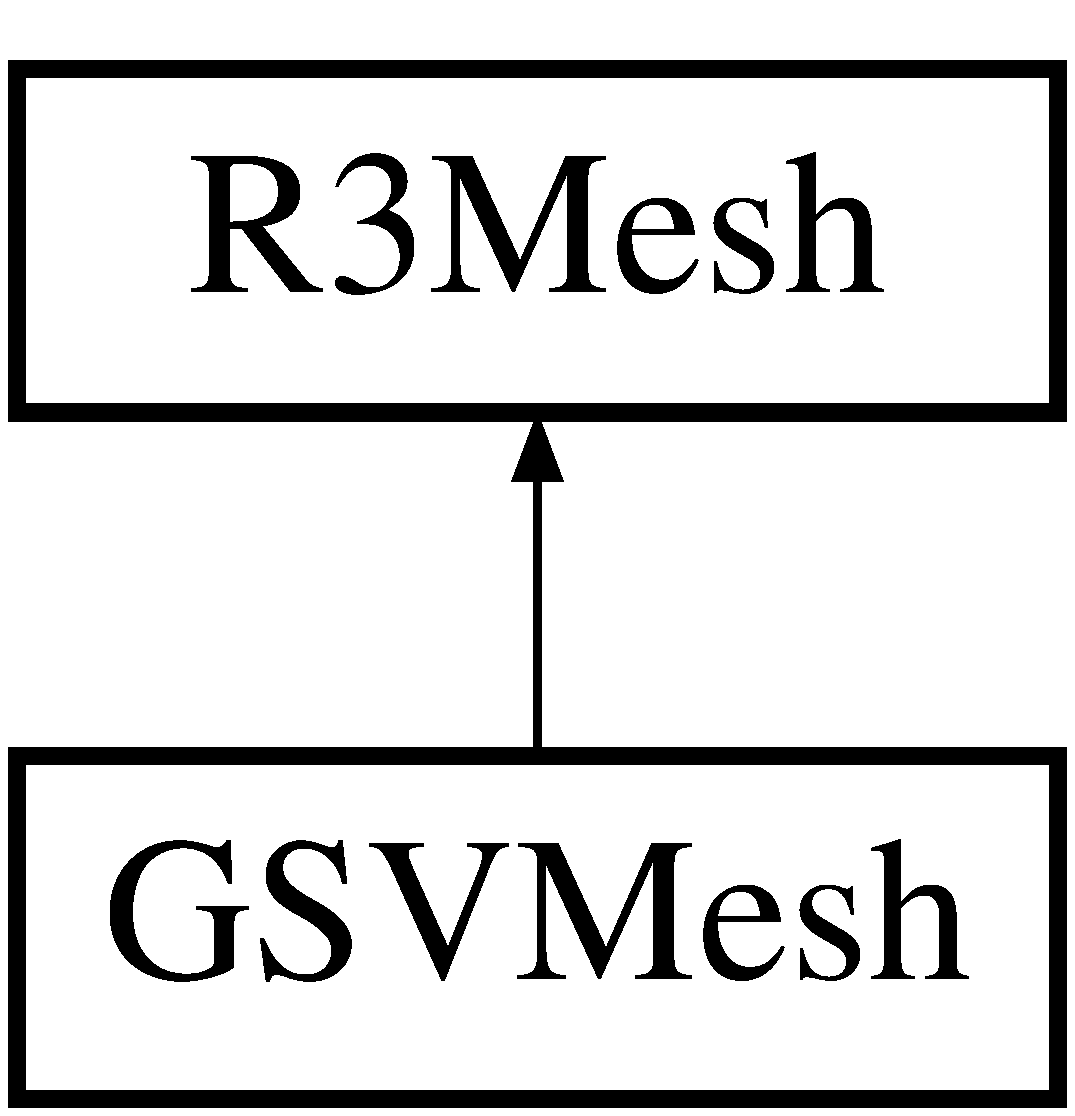
\includegraphics[height=2.000000cm]{class_g_s_v_mesh}
\end{center}
\end{figure}
\subsection*{Public Member Functions}
\begin{DoxyCompactItemize}
\item 
\hyperlink{class_g_s_v_scanline}{G\+S\+V\+Scanline} $\ast$ {\bfseries Vertex\+Scanline} (\hyperlink{class_r3_mesh_vertex}{R3\+Mesh\+Vertex} $\ast$vertex) const \hypertarget{class_g_s_v_mesh_a3b84f2a88828463f0043f7a727f230a8}{}\label{class_g_s_v_mesh_a3b84f2a88828463f0043f7a727f230a8}

\item 
R\+N\+Scalar {\bfseries Vertex\+Timestamp} (\hyperlink{class_r3_mesh_vertex}{R3\+Mesh\+Vertex} $\ast$vertex) const \hypertarget{class_g_s_v_mesh_a5da24209e27df3dbe3f60e229f72a1f1}{}\label{class_g_s_v_mesh_a5da24209e27df3dbe3f60e229f72a1f1}

\item 
R\+N\+Scalar {\bfseries Vertex\+Height} (\hyperlink{class_r3_mesh_vertex}{R3\+Mesh\+Vertex} $\ast$vertex) const \hypertarget{class_g_s_v_mesh_a875fb9d6f018d4b2863924dcda4b5659}{}\label{class_g_s_v_mesh_a875fb9d6f018d4b2863924dcda4b5659}

\item 
R\+N\+Scalar {\bfseries Vertex\+Laser\+Angle} (\hyperlink{class_r3_mesh_vertex}{R3\+Mesh\+Vertex} $\ast$vertex) const \hypertarget{class_g_s_v_mesh_ac4399a5ad8392efd8739fd210693d42d}{}\label{class_g_s_v_mesh_ac4399a5ad8392efd8739fd210693d42d}

\item 
R\+N\+Scalar {\bfseries Vertex\+Laser\+Depth} (\hyperlink{class_r3_mesh_vertex}{R3\+Mesh\+Vertex} $\ast$vertex) const \hypertarget{class_g_s_v_mesh_abf70269575cb0c5052583ed27034decd}{}\label{class_g_s_v_mesh_abf70269575cb0c5052583ed27034decd}

\item 
R\+N\+Scalar {\bfseries Vertex\+Laser\+Distance} (\hyperlink{class_r3_mesh_vertex}{R3\+Mesh\+Vertex} $\ast$vertex) const \hypertarget{class_g_s_v_mesh_a966c4a17ac4596af71d20e4a44386e33}{}\label{class_g_s_v_mesh_a966c4a17ac4596af71d20e4a44386e33}

\item 
\hyperlink{class_r3_point}{R3\+Point} {\bfseries Vertex\+Laser\+Viewpoint} (\hyperlink{class_r3_mesh_vertex}{R3\+Mesh\+Vertex} $\ast$vertex) const \hypertarget{class_g_s_v_mesh_a2c3170c3398e13ea8c0f6e65ae692e51}{}\label{class_g_s_v_mesh_a2c3170c3398e13ea8c0f6e65ae692e51}

\item 
\hyperlink{class_r3_vector}{R3\+Vector} {\bfseries Vertex\+Laser\+Towards} (\hyperlink{class_r3_mesh_vertex}{R3\+Mesh\+Vertex} $\ast$vertex) const \hypertarget{class_g_s_v_mesh_a528b086b605362d736e1ea71476fe008}{}\label{class_g_s_v_mesh_a528b086b605362d736e1ea71476fe008}

\item 
\hyperlink{class_r3_vector}{R3\+Vector} {\bfseries Vertex\+Laser\+Up} (\hyperlink{class_r3_mesh_vertex}{R3\+Mesh\+Vertex} $\ast$vertex) const \hypertarget{class_g_s_v_mesh_a7b2ade12d1f9b244fd6f0d42b0c6b2e1}{}\label{class_g_s_v_mesh_a7b2ade12d1f9b244fd6f0d42b0c6b2e1}

\item 
int {\bfseries Vertex\+Scanline\+Index} (\hyperlink{class_r3_mesh_vertex}{R3\+Mesh\+Vertex} $\ast$vertex) const \hypertarget{class_g_s_v_mesh_a5dfa68d12d34f6bb0452bcba92adb219}{}\label{class_g_s_v_mesh_a5dfa68d12d34f6bb0452bcba92adb219}

\item 
int {\bfseries Vertex\+Point\+Index} (\hyperlink{class_r3_mesh_vertex}{R3\+Mesh\+Vertex} $\ast$vertex) const \hypertarget{class_g_s_v_mesh_a534b9ebcd3c8792e2747536f335b0de0}{}\label{class_g_s_v_mesh_a534b9ebcd3c8792e2747536f335b0de0}

\item 
int {\bfseries Vertex\+Boundary\+Type} (\hyperlink{class_r3_mesh_vertex}{R3\+Mesh\+Vertex} $\ast$vertex) const \hypertarget{class_g_s_v_mesh_a78263085694901117ee084ad5e4b52c1}{}\label{class_g_s_v_mesh_a78263085694901117ee084ad5e4b52c1}

\item 
int {\bfseries Load\+Scan} (\hyperlink{class_g_s_v_scan}{G\+S\+V\+Scan} $\ast$scan, R\+N\+Length min\+\_\+viewpoint\+\_\+movement=0.\+05, R\+N\+Length max\+\_\+depth\+\_\+discontinuity=1)\hypertarget{class_g_s_v_mesh_af3b7a73b0e5f36ef106de1531f5f516d}{}\label{class_g_s_v_mesh_af3b7a73b0e5f36ef106de1531f5f516d}

\item 
virtual int {\bfseries Read\+Ply\+File} (\hyperlink{class_g_s_v_scan}{G\+S\+V\+Scan} $\ast$scan, const char $\ast$filename)\hypertarget{class_g_s_v_mesh_a3fae4ae5bbb3bd888da2251e953d4261}{}\label{class_g_s_v_mesh_a3fae4ae5bbb3bd888da2251e953d4261}

\item 
virtual int {\bfseries Write\+Ply\+File} (\hyperlink{class_g_s_v_scan}{G\+S\+V\+Scan} $\ast$scan, const char $\ast$filename, R\+N\+Boolean binary=T\+R\+UE)\hypertarget{class_g_s_v_mesh_a0783b16d93c397e4c8e18f3e54b7161b}{}\label{class_g_s_v_mesh_a0783b16d93c397e4c8e18f3e54b7161b}

\item 
virtual int {\bfseries Write\+A\+R\+F\+F\+File} (\hyperlink{class_g_s_v_scan}{G\+S\+V\+Scan} $\ast$scan, const char $\ast$filename)\hypertarget{class_g_s_v_mesh_a83fae5404000dc89fb3c9982bd1b5221}{}\label{class_g_s_v_mesh_a83fae5404000dc89fb3c9982bd1b5221}

\item 
\hyperlink{class_g_s_v_mesh_vertex}{G\+S\+V\+Mesh\+Vertex} $\ast$ {\bfseries Vertex} (int k) const \hypertarget{class_g_s_v_mesh_aa76e1ab14bdac3e1c426e8bd34d98b6e}{}\label{class_g_s_v_mesh_aa76e1ab14bdac3e1c426e8bd34d98b6e}

\item 
\hyperlink{class_g_s_v_mesh_vertex}{G\+S\+V\+Mesh\+Vertex} $\ast$ {\bfseries Vertex\+On\+Vertex} (const \hyperlink{class_r3_mesh_vertex}{R3\+Mesh\+Vertex} $\ast$vertex) const \hypertarget{class_g_s_v_mesh_a8e93864d1ebfe0949ef500e18038b55b}{}\label{class_g_s_v_mesh_a8e93864d1ebfe0949ef500e18038b55b}

\item 
\hyperlink{class_g_s_v_mesh_vertex}{G\+S\+V\+Mesh\+Vertex} $\ast$ {\bfseries Vertex\+On\+Vertex} (const \hyperlink{class_r3_mesh_vertex}{R3\+Mesh\+Vertex} $\ast$vertex, int k) const \hypertarget{class_g_s_v_mesh_a65e06249b8b2cbeba9bdb0a50d765058}{}\label{class_g_s_v_mesh_a65e06249b8b2cbeba9bdb0a50d765058}

\item 
\hyperlink{class_g_s_v_mesh_vertex}{G\+S\+V\+Mesh\+Vertex} $\ast$ {\bfseries Vertex\+On\+Edge} (const \hyperlink{class_r3_mesh_edge}{R3\+Mesh\+Edge} $\ast$edge) const \hypertarget{class_g_s_v_mesh_a813f93478de4fdd477c80ce7c3df4751}{}\label{class_g_s_v_mesh_a813f93478de4fdd477c80ce7c3df4751}

\item 
\hyperlink{class_g_s_v_mesh_vertex}{G\+S\+V\+Mesh\+Vertex} $\ast$ {\bfseries Vertex\+On\+Edge} (const \hyperlink{class_r3_mesh_edge}{R3\+Mesh\+Edge} $\ast$edge, int k) const \hypertarget{class_g_s_v_mesh_abe8ef82dc24c3c631987244d794e5b0f}{}\label{class_g_s_v_mesh_abe8ef82dc24c3c631987244d794e5b0f}

\item 
\hyperlink{class_g_s_v_mesh_vertex}{G\+S\+V\+Mesh\+Vertex} $\ast$ {\bfseries Vertex\+Across\+Edge} (const \hyperlink{class_r3_mesh_edge}{R3\+Mesh\+Edge} $\ast$edge, const \hyperlink{class_r3_mesh_vertex}{R3\+Mesh\+Vertex} $\ast$vertex) const \hypertarget{class_g_s_v_mesh_a11322e655e8d70ca199bdad404fc50f3}{}\label{class_g_s_v_mesh_a11322e655e8d70ca199bdad404fc50f3}

\item 
\hyperlink{class_g_s_v_mesh_vertex}{G\+S\+V\+Mesh\+Vertex} $\ast$ {\bfseries Vertex\+Between\+Edges} (const \hyperlink{class_r3_mesh_edge}{R3\+Mesh\+Edge} $\ast$edge1, const \hyperlink{class_r3_mesh_edge}{R3\+Mesh\+Edge} $\ast$edge2) const \hypertarget{class_g_s_v_mesh_ab9813be1dd59e798e8ab4354210408ff}{}\label{class_g_s_v_mesh_ab9813be1dd59e798e8ab4354210408ff}

\item 
\hyperlink{class_g_s_v_mesh_vertex}{G\+S\+V\+Mesh\+Vertex} $\ast$ {\bfseries Vertex\+On\+Edge} (const \hyperlink{class_r3_mesh_edge}{R3\+Mesh\+Edge} $\ast$edge, const \hyperlink{class_r3_mesh_face}{R3\+Mesh\+Face} $\ast$face, R\+N\+Direction dir=R\+N\+\_\+\+C\+CW) const \hypertarget{class_g_s_v_mesh_a3691d027a79c6bade16de6186860df06}{}\label{class_g_s_v_mesh_a3691d027a79c6bade16de6186860df06}

\item 
\hyperlink{class_g_s_v_mesh_vertex}{G\+S\+V\+Mesh\+Vertex} $\ast$ {\bfseries Vertex\+On\+Face} (const \hyperlink{class_r3_mesh_face}{R3\+Mesh\+Face} $\ast$face) const \hypertarget{class_g_s_v_mesh_a47c840cfca3849706b7227fe84f850bc}{}\label{class_g_s_v_mesh_a47c840cfca3849706b7227fe84f850bc}

\item 
\hyperlink{class_g_s_v_mesh_vertex}{G\+S\+V\+Mesh\+Vertex} $\ast$ {\bfseries Vertex\+On\+Face} (const \hyperlink{class_r3_mesh_face}{R3\+Mesh\+Face} $\ast$face, int k) const \hypertarget{class_g_s_v_mesh_aab837bdf946fab5e7824bd035f3a5004}{}\label{class_g_s_v_mesh_aab837bdf946fab5e7824bd035f3a5004}

\item 
\hyperlink{class_g_s_v_mesh_vertex}{G\+S\+V\+Mesh\+Vertex} $\ast$ {\bfseries Vertex\+On\+Face} (const \hyperlink{class_r3_mesh_face}{R3\+Mesh\+Face} $\ast$face, const \hyperlink{class_r3_mesh_vertex}{R3\+Mesh\+Vertex} $\ast$vertex, R\+N\+Direction dir=R\+N\+\_\+\+C\+CW) const \hypertarget{class_g_s_v_mesh_a34f061f3d367bab9a4541f84ba31aa3e}{}\label{class_g_s_v_mesh_a34f061f3d367bab9a4541f84ba31aa3e}

\item 
\hyperlink{class_g_s_v_mesh_vertex}{G\+S\+V\+Mesh\+Vertex} $\ast$ {\bfseries Vertex\+On\+Face} (const \hyperlink{class_r3_mesh_face}{R3\+Mesh\+Face} $\ast$face, const \hyperlink{class_r3_mesh_edge}{R3\+Mesh\+Edge} $\ast$edge, R\+N\+Direction dir=R\+N\+\_\+\+C\+CW) const \hypertarget{class_g_s_v_mesh_a3b1caffaaa2ec1d7dcd056b36a161830}{}\label{class_g_s_v_mesh_a3b1caffaaa2ec1d7dcd056b36a161830}

\item 
\hyperlink{class_g_s_v_mesh_vertex}{G\+S\+V\+Mesh\+Vertex} $\ast$ {\bfseries Vertex\+Across\+Face} (const \hyperlink{class_r3_mesh_face}{R3\+Mesh\+Face} $\ast$face, const \hyperlink{class_r3_mesh_edge}{R3\+Mesh\+Edge} $\ast$edge) const \hypertarget{class_g_s_v_mesh_a20343b61ca9442eb4945adcd76a53941}{}\label{class_g_s_v_mesh_a20343b61ca9442eb4945adcd76a53941}

\item 
\hyperlink{class_g_s_v_mesh_vertex}{G\+S\+V\+Mesh\+Vertex} $\ast$ {\bfseries Vertex\+Between\+Faces} (const \hyperlink{class_r3_mesh_face}{R3\+Mesh\+Face} $\ast$face1, const \hyperlink{class_r3_mesh_face}{R3\+Mesh\+Face} $\ast$face2, R\+N\+Direction dir=R\+N\+\_\+\+C\+CW) const \hypertarget{class_g_s_v_mesh_aa3d1c1a04c86e330d6075b5374e9c529}{}\label{class_g_s_v_mesh_aa3d1c1a04c86e330d6075b5374e9c529}

\item 
virtual \hyperlink{class_g_s_v_mesh_vertex}{G\+S\+V\+Mesh\+Vertex} $\ast$ {\bfseries Merge\+Vertex} (\hyperlink{class_r3_mesh_vertex}{R3\+Mesh\+Vertex} $\ast$v1, \hyperlink{class_r3_mesh_vertex}{R3\+Mesh\+Vertex} $\ast$v2)\hypertarget{class_g_s_v_mesh_a4b271c421a7dd1741f7ce5e3c1bf60a6}{}\label{class_g_s_v_mesh_a4b271c421a7dd1741f7ce5e3c1bf60a6}

\item 
virtual \hyperlink{class_g_s_v_mesh_vertex}{G\+S\+V\+Mesh\+Vertex} $\ast$ {\bfseries Collapse\+Edge} (\hyperlink{class_r3_mesh_edge}{R3\+Mesh\+Edge} $\ast$edge, const \hyperlink{class_r3_point}{R3\+Point} \&point)\hypertarget{class_g_s_v_mesh_aa2f4cf7614c8bc3bdd0382dc34f9f19f}{}\label{class_g_s_v_mesh_aa2f4cf7614c8bc3bdd0382dc34f9f19f}

\item 
virtual \hyperlink{class_g_s_v_mesh_vertex}{G\+S\+V\+Mesh\+Vertex} $\ast$ {\bfseries Collapse\+Face} (\hyperlink{class_r3_mesh_face}{R3\+Mesh\+Face} $\ast$face, const \hyperlink{class_r3_point}{R3\+Point} \&point)\hypertarget{class_g_s_v_mesh_ae6d11bb1fe286c0f6ca45d9b6e7fe2e8}{}\label{class_g_s_v_mesh_ae6d11bb1fe286c0f6ca45d9b6e7fe2e8}

\item 
virtual \hyperlink{class_g_s_v_mesh_vertex}{G\+S\+V\+Mesh\+Vertex} $\ast$ {\bfseries Collapse\+Edge} (\hyperlink{class_r3_mesh_edge}{R3\+Mesh\+Edge} $\ast$edge)\hypertarget{class_g_s_v_mesh_a2bce05c396e58b42129dd82bb74cde44}{}\label{class_g_s_v_mesh_a2bce05c396e58b42129dd82bb74cde44}

\item 
virtual \hyperlink{class_g_s_v_mesh_vertex}{G\+S\+V\+Mesh\+Vertex} $\ast$ {\bfseries Collapse\+Face} (\hyperlink{class_r3_mesh_face}{R3\+Mesh\+Face} $\ast$face)\hypertarget{class_g_s_v_mesh_aa023f776cfd9c6046b602b7a31eac216}{}\label{class_g_s_v_mesh_aa023f776cfd9c6046b602b7a31eac216}

\item 
virtual \hyperlink{class_g_s_v_mesh_vertex}{G\+S\+V\+Mesh\+Vertex} $\ast$ {\bfseries Split\+Edge} (\hyperlink{class_r3_mesh_edge}{R3\+Mesh\+Edge} $\ast$edge, const \hyperlink{class_r3_point}{R3\+Point} \&point, \hyperlink{class_r3_mesh_edge}{R3\+Mesh\+Edge} $\ast$$\ast$e0=N\+U\+LL, \hyperlink{class_r3_mesh_edge}{R3\+Mesh\+Edge} $\ast$$\ast$e1=N\+U\+LL)\hypertarget{class_g_s_v_mesh_aef8080a94f153225f77b793f74f888c8}{}\label{class_g_s_v_mesh_aef8080a94f153225f77b793f74f888c8}

\item 
virtual \hyperlink{class_g_s_v_mesh_vertex}{G\+S\+V\+Mesh\+Vertex} $\ast$ {\bfseries Split\+Edge} (\hyperlink{class_r3_mesh_edge}{R3\+Mesh\+Edge} $\ast$edge, const \hyperlink{class_r3_plane}{R3\+Plane} \&plane)\hypertarget{class_g_s_v_mesh_aa2c1c78345b1f19febf5f102f452e4d4}{}\label{class_g_s_v_mesh_aa2c1c78345b1f19febf5f102f452e4d4}

\item 
virtual \hyperlink{class_g_s_v_mesh_vertex}{G\+S\+V\+Mesh\+Vertex} $\ast$ {\bfseries Subdivide\+Edge} (\hyperlink{class_r3_mesh_edge}{R3\+Mesh\+Edge} $\ast$edge)\hypertarget{class_g_s_v_mesh_a25e6e1790db8fdd6b8025e1bd8d48fb4}{}\label{class_g_s_v_mesh_a25e6e1790db8fdd6b8025e1bd8d48fb4}

\item 
virtual \hyperlink{class_g_s_v_mesh_vertex}{G\+S\+V\+Mesh\+Vertex} $\ast$ {\bfseries Split\+Face} (\hyperlink{class_r3_mesh_face}{R3\+Mesh\+Face} $\ast$face, const \hyperlink{class_r3_point}{R3\+Point} \&point, \hyperlink{class_r3_mesh_face}{R3\+Mesh\+Face} $\ast$$\ast$f0=N\+U\+LL, \hyperlink{class_r3_mesh_face}{R3\+Mesh\+Face} $\ast$$\ast$f1=N\+U\+LL, \hyperlink{class_r3_mesh_face}{R3\+Mesh\+Face} $\ast$$\ast$f2=N\+U\+LL)\hypertarget{class_g_s_v_mesh_a9de7be7a3fb017fb02a362debbb72367}{}\label{class_g_s_v_mesh_a9de7be7a3fb017fb02a362debbb72367}

\item 
virtual \hyperlink{class_r3_mesh_vertex}{R3\+Mesh\+Vertex} $\ast$ {\bfseries Create\+Vertex} (const \hyperlink{class_r3_point}{R3\+Point} \&position, \hyperlink{class_r3_mesh_vertex}{R3\+Mesh\+Vertex} $\ast$vertex=N\+U\+LL)\hypertarget{class_g_s_v_mesh_ab463d9a27c032686d21fac9f37baa54d}{}\label{class_g_s_v_mesh_ab463d9a27c032686d21fac9f37baa54d}

\item 
virtual \hyperlink{class_r3_mesh_vertex}{R3\+Mesh\+Vertex} $\ast$ {\bfseries Create\+Vertex} (const \hyperlink{class_r3_point}{R3\+Point} \&position, const \hyperlink{class_r3_vector}{R3\+Vector} \&normal, \hyperlink{class_r3_mesh_vertex}{R3\+Mesh\+Vertex} $\ast$vertex=N\+U\+LL)\hypertarget{class_g_s_v_mesh_a2f403b41f8c57b88b4c568d85b626172}{}\label{class_g_s_v_mesh_a2f403b41f8c57b88b4c568d85b626172}

\item 
virtual R3\+Mesh\+Type {\bfseries Intersection} (const \hyperlink{class_r3_ray}{R3\+Ray} \&ray, \hyperlink{struct_r3_mesh_intersection}{R3\+Mesh\+Intersection} $\ast$intersection=N\+U\+LL, R\+N\+Scalar min\+\_\+t=0, R\+N\+Scalar max\+\_\+t=R\+N\+\_\+\+I\+N\+F\+I\+N\+I\+TY, int($\ast$Is\+Compatible)(const \hyperlink{class_r3_point}{R3\+Point} \&, const \hyperlink{class_r3_vector}{R3\+Vector} \&, \hyperlink{class_r3_mesh}{R3\+Mesh} $\ast$, \hyperlink{class_r3_mesh_face}{R3\+Mesh\+Face} $\ast$, void $\ast$)=N\+U\+LL, void $\ast$compatible\+\_\+data=N\+U\+LL) const \hypertarget{class_g_s_v_mesh_a8d6c147e6459c0e1754bee937cadfea3}{}\label{class_g_s_v_mesh_a8d6c147e6459c0e1754bee937cadfea3}

\item 
virtual R3\+Mesh\+Type {\bfseries Closest\+Point} (const \hyperlink{class_r3_point}{R3\+Point} \&query, \hyperlink{struct_r3_mesh_intersection}{R3\+Mesh\+Intersection} $\ast$closest=N\+U\+LL, R\+N\+Scalar min\+\_\+distance=0, R\+N\+Scalar max\+\_\+distance=R\+N\+\_\+\+I\+N\+F\+I\+N\+I\+TY, int($\ast$Is\+Compatible)(const \hyperlink{class_r3_point}{R3\+Point} \&, const \hyperlink{class_r3_vector}{R3\+Vector} \&, \hyperlink{class_r3_mesh}{R3\+Mesh} $\ast$, \hyperlink{class_r3_mesh_face}{R3\+Mesh\+Face} $\ast$, void $\ast$)=N\+U\+LL, void $\ast$compatible\+\_\+data=N\+U\+LL)\hypertarget{class_g_s_v_mesh_acdfcf0811ef54cb0eb97bae8585e68b1}{}\label{class_g_s_v_mesh_acdfcf0811ef54cb0eb97bae8585e68b1}

\item 
virtual R3\+Mesh\+Type {\bfseries Intersection} (const \hyperlink{class_r3_ray}{R3\+Ray} \&ray, G\+S\+V\+Mesh\+Face $\ast$face, \hyperlink{struct_r3_mesh_intersection}{R3\+Mesh\+Intersection} $\ast$intersection=N\+U\+LL) const \hypertarget{class_g_s_v_mesh_aeba185c3abfee585f68001be68648a80}{}\label{class_g_s_v_mesh_aeba185c3abfee585f68001be68648a80}

\item 
virtual void {\bfseries Draw} (R\+N\+Boolean texture\+\_\+coordinates) const \hypertarget{class_g_s_v_mesh_a05467ac91e535dd69b904d8e71291e6f}{}\label{class_g_s_v_mesh_a05467ac91e535dd69b904d8e71291e6f}

\item 
virtual void {\bfseries Draw} (void) const \hypertarget{class_g_s_v_mesh_a83d37a551b6c5106cf8e8550b1c42fef}{}\label{class_g_s_v_mesh_a83d37a551b6c5106cf8e8550b1c42fef}

\end{DoxyCompactItemize}
\subsection*{Protected Attributes}
\begin{DoxyCompactItemize}
\item 
\hyperlink{class_g_s_v_mesh_vertex}{G\+S\+V\+Mesh\+Vertex} $\ast$ {\bfseries gsv\+\_\+vertex\+\_\+block}\hypertarget{class_g_s_v_mesh_a496ee13f368242f1575827285fc615a0}{}\label{class_g_s_v_mesh_a496ee13f368242f1575827285fc615a0}

\item 
\hyperlink{class_r3_mesh_search_tree}{R3\+Mesh\+Search\+Tree} $\ast$ {\bfseries search\+\_\+tree}\hypertarget{class_g_s_v_mesh_a12a8557cf89e4277909c9441bb43970f}{}\label{class_g_s_v_mesh_a12a8557cf89e4277909c9441bb43970f}

\end{DoxyCompactItemize}
\subsection*{Additional Inherited Members}


The documentation for this class was generated from the following files\+:\begin{DoxyCompactItemize}
\item 
G\+S\+V/G\+S\+V\+Mesh.\+h\item 
G\+S\+V/G\+S\+V\+Mesh.\+cpp\end{DoxyCompactItemize}

\hypertarget{class_g_s_v_mesh_vertex}{}\section{G\+S\+V\+Mesh\+Vertex Class Reference}
\label{class_g_s_v_mesh_vertex}\index{G\+S\+V\+Mesh\+Vertex@{G\+S\+V\+Mesh\+Vertex}}
Inheritance diagram for G\+S\+V\+Mesh\+Vertex\+:\begin{figure}[H]
\begin{center}
\leavevmode
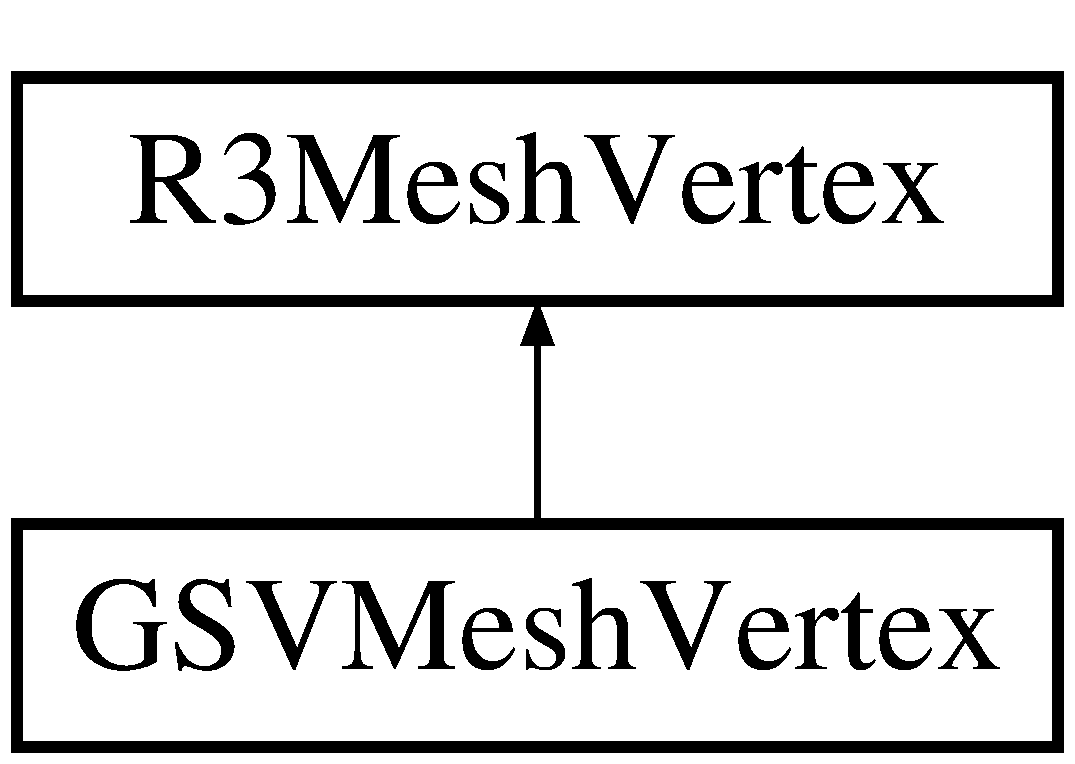
\includegraphics[height=2.000000cm]{class_g_s_v_mesh_vertex}
\end{center}
\end{figure}
\subsection*{Friends}
\begin{DoxyCompactItemize}
\item 
class {\bfseries G\+S\+V\+Mesh}\hypertarget{class_g_s_v_mesh_vertex_a55b925404bd0cfd37a19a5aa648ec5e3}{}\label{class_g_s_v_mesh_vertex_a55b925404bd0cfd37a19a5aa648ec5e3}

\end{DoxyCompactItemize}
\subsection*{Additional Inherited Members}


The documentation for this class was generated from the following files\+:\begin{DoxyCompactItemize}
\item 
G\+S\+V/G\+S\+V\+Mesh.\+h\item 
G\+S\+V/G\+S\+V\+Mesh.\+cpp\end{DoxyCompactItemize}

\hypertarget{class_g_s_v_panorama}{}\section{G\+S\+V\+Panorama Class Reference}
\label{class_g_s_v_panorama}\index{G\+S\+V\+Panorama@{G\+S\+V\+Panorama}}
\subsection*{Public Member Functions}
\begin{DoxyCompactItemize}
\item 
\hyperlink{class_g_s_v_scene}{G\+S\+V\+Scene} $\ast$ {\bfseries Scene} (void) const \hypertarget{class_g_s_v_panorama_ab86070f64ea38217ace866e0677f9095}{}\label{class_g_s_v_panorama_ab86070f64ea38217ace866e0677f9095}

\item 
int {\bfseries Scene\+Index} (void) const \hypertarget{class_g_s_v_panorama_a8e97213ba5eec4bcfe880c4d70e6ace9}{}\label{class_g_s_v_panorama_a8e97213ba5eec4bcfe880c4d70e6ace9}

\item 
\hyperlink{class_g_s_v_run}{G\+S\+V\+Run} $\ast$ {\bfseries Run} (void) const \hypertarget{class_g_s_v_panorama_a7c6b4767930ac31d662ea498394a526e}{}\label{class_g_s_v_panorama_a7c6b4767930ac31d662ea498394a526e}

\item 
int {\bfseries Run\+Index} (void) const \hypertarget{class_g_s_v_panorama_ab30123d6188a792ded266603b815bec9}{}\label{class_g_s_v_panorama_ab30123d6188a792ded266603b815bec9}

\item 
\hyperlink{class_g_s_v_segment}{G\+S\+V\+Segment} $\ast$ {\bfseries Segment} (void) const \hypertarget{class_g_s_v_panorama_a26ccdc213efb2f952e074d6705102fe5}{}\label{class_g_s_v_panorama_a26ccdc213efb2f952e074d6705102fe5}

\item 
int {\bfseries Segment\+Index} (void) const \hypertarget{class_g_s_v_panorama_accf0027fbd436f5625b8400c61dee07a}{}\label{class_g_s_v_panorama_accf0027fbd436f5625b8400c61dee07a}

\item 
int {\bfseries N\+Images} (void) const \hypertarget{class_g_s_v_panorama_a3744a6f7219a77b436492b6603434aa4}{}\label{class_g_s_v_panorama_a3744a6f7219a77b436492b6603434aa4}

\item 
\hyperlink{class_g_s_v_image}{G\+S\+V\+Image} $\ast$ {\bfseries Image} (int image\+\_\+index) const \hypertarget{class_g_s_v_panorama_a1ef7000c20100b09cce0c273937e5fb6}{}\label{class_g_s_v_panorama_a1ef7000c20100b09cce0c273937e5fb6}

\item 
const \hyperlink{class_r3_point}{R3\+Point} \& {\bfseries Viewpoint} (void) const \hypertarget{class_g_s_v_panorama_a186b389bd1eb14c6239f412d84b38700}{}\label{class_g_s_v_panorama_a186b389bd1eb14c6239f412d84b38700}

\item 
R\+N\+Scalar {\bfseries Timestamp} (void) const \hypertarget{class_g_s_v_panorama_a495245191b984a3724644e776015f6ea}{}\label{class_g_s_v_panorama_a495245191b984a3724644e776015f6ea}

\item 
void $\ast$ {\bfseries Data} (void) const \hypertarget{class_g_s_v_panorama_ae7419f220b95eb0401c5a7ca66f530d4}{}\label{class_g_s_v_panorama_ae7419f220b95eb0401c5a7ca66f530d4}

\item 
void {\bfseries Insert\+Image} (\hyperlink{class_g_s_v_image}{G\+S\+V\+Image} $\ast$image)\hypertarget{class_g_s_v_panorama_a7c0115455425fa77fb4c15fde8b61bc0}{}\label{class_g_s_v_panorama_a7c0115455425fa77fb4c15fde8b61bc0}

\item 
void {\bfseries Remove\+Image} (\hyperlink{class_g_s_v_image}{G\+S\+V\+Image} $\ast$image)\hypertarget{class_g_s_v_panorama_a5c7ccdf49fff0decaf6d2b6da7fa22c2}{}\label{class_g_s_v_panorama_a5c7ccdf49fff0decaf6d2b6da7fa22c2}

\item 
void {\bfseries Set\+Viewpoint} (const \hyperlink{class_r3_point}{R3\+Point} \&viewpoint)\hypertarget{class_g_s_v_panorama_a1f8b29f2deb1f96fc1f5876e7eaeb8cd}{}\label{class_g_s_v_panorama_a1f8b29f2deb1f96fc1f5876e7eaeb8cd}

\item 
void {\bfseries Set\+Timestamp} (R\+N\+Scalar timestamp)\hypertarget{class_g_s_v_panorama_ad32c31d645d92e4a4b3d9a6af21f352b}{}\label{class_g_s_v_panorama_ad32c31d645d92e4a4b3d9a6af21f352b}

\item 
void {\bfseries Set\+Data} (void $\ast$data)\hypertarget{class_g_s_v_panorama_a62c00d3dbe71bacf0473dd6456fb88aa}{}\label{class_g_s_v_panorama_a62c00d3dbe71bacf0473dd6456fb88aa}

\item 
virtual void {\bfseries Draw} (\hyperlink{class_r_n_flags}{R\+N\+Flags} flags=G\+S\+V\+\_\+\+D\+E\+F\+A\+U\+L\+T\+\_\+\+D\+R\+A\+W\+\_\+\+F\+L\+A\+GS) const \hypertarget{class_g_s_v_panorama_a96249e8420043b26f23c22e524a26572}{}\label{class_g_s_v_panorama_a96249e8420043b26f23c22e524a26572}

\item 
virtual void {\bfseries Print} (F\+I\+LE $\ast$fp=N\+U\+LL, const char $\ast$prefix=N\+U\+LL, const char $\ast$suffix=N\+U\+LL) const \hypertarget{class_g_s_v_panorama_adceb3e87bf49a16dde460380fa65e621}{}\label{class_g_s_v_panorama_adceb3e87bf49a16dde460380fa65e621}

\item 
void {\bfseries Update\+Viewpoint} (void)\hypertarget{class_g_s_v_panorama_a46d254e7a14d63b32dce03e287406bcb}{}\label{class_g_s_v_panorama_a46d254e7a14d63b32dce03e287406bcb}

\item 
void {\bfseries Update\+Timestamp} (void)\hypertarget{class_g_s_v_panorama_ac9b1b76f1eaf751cf99bf0b47f65f10f}{}\label{class_g_s_v_panorama_ac9b1b76f1eaf751cf99bf0b47f65f10f}

\end{DoxyCompactItemize}
\subsection*{Protected Attributes}
\begin{DoxyCompactItemize}
\item 
\hyperlink{class_g_s_v_segment}{G\+S\+V\+Segment} $\ast$ {\bfseries segment}\hypertarget{class_g_s_v_panorama_a13c99d4d5f144ed76b082b2938730ce4}{}\label{class_g_s_v_panorama_a13c99d4d5f144ed76b082b2938730ce4}

\item 
int {\bfseries segment\+\_\+index}\hypertarget{class_g_s_v_panorama_a8c0a2a54ca1f49edcad4c684e4778315}{}\label{class_g_s_v_panorama_a8c0a2a54ca1f49edcad4c684e4778315}

\item 
\hyperlink{class_r_n_array}{R\+N\+Array}$<$ \hyperlink{class_g_s_v_image}{G\+S\+V\+Image} $\ast$ $>$ {\bfseries images}\hypertarget{class_g_s_v_panorama_a73aeb6bf2e6861fd3dc9fb1cd53ea5ee}{}\label{class_g_s_v_panorama_a73aeb6bf2e6861fd3dc9fb1cd53ea5ee}

\item 
\hyperlink{class_r3_point}{R3\+Point} {\bfseries viewpoint}\hypertarget{class_g_s_v_panorama_ace1a80c21d180105ce1a61bb7d6d993e}{}\label{class_g_s_v_panorama_ace1a80c21d180105ce1a61bb7d6d993e}

\item 
R\+N\+Scalar {\bfseries timestamp}\hypertarget{class_g_s_v_panorama_acb69aaa8521fbc57afad0643b191cc84}{}\label{class_g_s_v_panorama_acb69aaa8521fbc57afad0643b191cc84}

\item 
void $\ast$ {\bfseries data}\hypertarget{class_g_s_v_panorama_adf0f6e0c6008c7f5b761a4064d2aefde}{}\label{class_g_s_v_panorama_adf0f6e0c6008c7f5b761a4064d2aefde}

\end{DoxyCompactItemize}
\subsection*{Friends}
\begin{DoxyCompactItemize}
\item 
class {\bfseries G\+S\+V\+Segment}\hypertarget{class_g_s_v_panorama_a24c71f4a2a67fb7c97d76dffafabda73}{}\label{class_g_s_v_panorama_a24c71f4a2a67fb7c97d76dffafabda73}

\end{DoxyCompactItemize}


The documentation for this class was generated from the following files\+:\begin{DoxyCompactItemize}
\item 
G\+S\+V/G\+S\+V\+Panorama.\+h\item 
G\+S\+V/G\+S\+V\+Panorama.\+cpp\end{DoxyCompactItemize}

\hypertarget{class_g_s_v_pose}{}\section{G\+S\+V\+Pose Class Reference}
\label{class_g_s_v_pose}\index{G\+S\+V\+Pose@{G\+S\+V\+Pose}}
\subsection*{Public Member Functions}
\begin{DoxyCompactItemize}
\item 
{\bfseries G\+S\+V\+Pose} (const \hyperlink{class_r3_point}{R3\+Point} \&viewpoint, const \hyperlink{class_r3_quaternion}{R3\+Quaternion} \&orientation)\hypertarget{class_g_s_v_pose_ad0325ddef2d0e8fd88cb0c6acd9e4a3e}{}\label{class_g_s_v_pose_ad0325ddef2d0e8fd88cb0c6acd9e4a3e}

\item 
{\bfseries G\+S\+V\+Pose} (double px, double py, double pz, double qx, double qy, double qz, double qw)\hypertarget{class_g_s_v_pose_a76a8e7936aad12e9f6915cd102486103}{}\label{class_g_s_v_pose_a76a8e7936aad12e9f6915cd102486103}

\item 
const \hyperlink{class_r3_point}{R3\+Point} \& {\bfseries Viewpoint} (void) const \hypertarget{class_g_s_v_pose_a9475be2716846027f8b6e4f4fc8ed89e}{}\label{class_g_s_v_pose_a9475be2716846027f8b6e4f4fc8ed89e}

\item 
const \hyperlink{class_r3_quaternion}{R3\+Quaternion} \& {\bfseries Orientation} (void) const \hypertarget{class_g_s_v_pose_a235dc10a7609c320911549ac03fa0a70}{}\label{class_g_s_v_pose_a235dc10a7609c320911549ac03fa0a70}

\item 
const \hyperlink{class_r3_vector}{R3\+Vector} {\bfseries Towards} (void) const \hypertarget{class_g_s_v_pose_a861d9166c2e892e3c1a5881d5b396108}{}\label{class_g_s_v_pose_a861d9166c2e892e3c1a5881d5b396108}

\item 
const \hyperlink{class_r3_vector}{R3\+Vector} {\bfseries Up} (void) const \hypertarget{class_g_s_v_pose_af99b5e2fa5d1de0ff090566d5dad80fd}{}\label{class_g_s_v_pose_af99b5e2fa5d1de0ff090566d5dad80fd}

\item 
const \hyperlink{class_r3_vector}{R3\+Vector} {\bfseries Right} (void) const \hypertarget{class_g_s_v_pose_af39180d7dbd68159cbc35e8ca2f9dcf2}{}\label{class_g_s_v_pose_af39180d7dbd68159cbc35e8ca2f9dcf2}

\item 
const \hyperlink{class_r4_matrix}{R4\+Matrix} {\bfseries Matrix} (void) const \hypertarget{class_g_s_v_pose_a33948aed7e8459cade083f0fdadc7e5c}{}\label{class_g_s_v_pose_a33948aed7e8459cade083f0fdadc7e5c}

\item 
void {\bfseries Set\+Viewpoint} (const \hyperlink{class_r3_point}{R3\+Point} \&position)\hypertarget{class_g_s_v_pose_a81122257c988666e9ad114f128479b50}{}\label{class_g_s_v_pose_a81122257c988666e9ad114f128479b50}

\item 
void {\bfseries Set\+Orientation} (const \hyperlink{class_r3_quaternion}{R3\+Quaternion} \&orientation)\hypertarget{class_g_s_v_pose_ac8e259a65512ad173fe4af9a6dd0b69b}{}\label{class_g_s_v_pose_ac8e259a65512ad173fe4af9a6dd0b69b}

\item 
void {\bfseries Translate} (const \hyperlink{class_r3_vector}{R3\+Vector} \&translation)\hypertarget{class_g_s_v_pose_a1a557a2b9cac48f9701934a0dc719787}{}\label{class_g_s_v_pose_a1a557a2b9cac48f9701934a0dc719787}

\item 
void {\bfseries Rotate} (const \hyperlink{class_r3_quaternion}{R3\+Quaternion} \&rotation)\hypertarget{class_g_s_v_pose_a91aff541579b48f72f19941184c1c048}{}\label{class_g_s_v_pose_a91aff541579b48f72f19941184c1c048}

\item 
void {\bfseries Rotate} (const \hyperlink{class_r3_vector}{R3\+Vector} \&xyz\+\_\+angles)\hypertarget{class_g_s_v_pose_af692e88240238e796cbaeedb6259c5d2}{}\label{class_g_s_v_pose_af692e88240238e796cbaeedb6259c5d2}

\item 
void {\bfseries Transform} (const \hyperlink{class_r3_affine}{R3\+Affine} \&affine)\hypertarget{class_g_s_v_pose_a59568bd5cbc3416b6535704a4a550bc5}{}\label{class_g_s_v_pose_a59568bd5cbc3416b6535704a4a550bc5}

\item 
virtual void {\bfseries Draw} (\hyperlink{class_r_n_flags}{R\+N\+Flags} flags=G\+S\+V\+\_\+\+D\+E\+F\+A\+U\+L\+T\+\_\+\+D\+R\+A\+W\+\_\+\+F\+L\+A\+GS) const \hypertarget{class_g_s_v_pose_a9f6cf50fd5c6ee49e8a6013a6b04644e}{}\label{class_g_s_v_pose_a9f6cf50fd5c6ee49e8a6013a6b04644e}

\item 
virtual void {\bfseries Print} (F\+I\+LE $\ast$fp=N\+U\+LL, const char $\ast$prefix=N\+U\+LL, const char $\ast$suffix=N\+U\+LL) const \hypertarget{class_g_s_v_pose_aa2d0f827f02b77f17fcd90a30f132dbe}{}\label{class_g_s_v_pose_aa2d0f827f02b77f17fcd90a30f132dbe}

\end{DoxyCompactItemize}
\subsection*{Protected Attributes}
\begin{DoxyCompactItemize}
\item 
\hyperlink{class_r3_point}{R3\+Point} {\bfseries viewpoint}\hypertarget{class_g_s_v_pose_aaed6ef8149b84b7da675028187c87b0f}{}\label{class_g_s_v_pose_aaed6ef8149b84b7da675028187c87b0f}

\item 
\hyperlink{class_r3_quaternion}{R3\+Quaternion} {\bfseries orientation}\hypertarget{class_g_s_v_pose_a8b51594a232f1240f2cf52c665340194}{}\label{class_g_s_v_pose_a8b51594a232f1240f2cf52c665340194}

\end{DoxyCompactItemize}


The documentation for this class was generated from the following files\+:\begin{DoxyCompactItemize}
\item 
G\+S\+V/G\+S\+V\+Pose.\+h\item 
G\+S\+V/G\+S\+V\+Pose.\+cpp\end{DoxyCompactItemize}

\hypertarget{class_g_s_v_run}{}\section{G\+S\+V\+Run Class Reference}
\label{class_g_s_v_run}\index{G\+S\+V\+Run@{G\+S\+V\+Run}}
\subsection*{Public Member Functions}
\begin{DoxyCompactItemize}
\item 
{\bfseries G\+S\+V\+Run} (const char $\ast$name=N\+U\+LL)\hypertarget{class_g_s_v_run_ac22793831e560f3c83c019a2451be01d}{}\label{class_g_s_v_run_ac22793831e560f3c83c019a2451be01d}

\item 
\hyperlink{class_g_s_v_scene}{G\+S\+V\+Scene} $\ast$ {\bfseries Scene} (void) const \hypertarget{class_g_s_v_run_af28052620e0bdcb553d583e920110214}{}\label{class_g_s_v_run_af28052620e0bdcb553d583e920110214}

\item 
int {\bfseries Scene\+Index} (void) const \hypertarget{class_g_s_v_run_a8662d1650d4448f58af71ebc3e1982f7}{}\label{class_g_s_v_run_a8662d1650d4448f58af71ebc3e1982f7}

\item 
int {\bfseries N\+Segments} (void) const \hypertarget{class_g_s_v_run_a80533a17968821897c8237cd6b0c9f40}{}\label{class_g_s_v_run_a80533a17968821897c8237cd6b0c9f40}

\item 
\hyperlink{class_g_s_v_segment}{G\+S\+V\+Segment} $\ast$ {\bfseries Segment} (int segment\+\_\+index) const \hypertarget{class_g_s_v_run_af66bb48cce46ac88d2116b4da3f350d9}{}\label{class_g_s_v_run_af66bb48cce46ac88d2116b4da3f350d9}

\item 
int {\bfseries N\+Cameras} (void) const \hypertarget{class_g_s_v_run_a73485909ac78226625208fa7dbebdecb}{}\label{class_g_s_v_run_a73485909ac78226625208fa7dbebdecb}

\item 
\hyperlink{class_g_s_v_camera}{G\+S\+V\+Camera} $\ast$ {\bfseries Camera} (int index) const \hypertarget{class_g_s_v_run_aedb825ba60bd68a048e25d88fc6c6910}{}\label{class_g_s_v_run_aedb825ba60bd68a048e25d88fc6c6910}

\item 
int {\bfseries N\+Lasers} (void) const \hypertarget{class_g_s_v_run_a745fe72cfc5a17293a71c327ffdad3ee}{}\label{class_g_s_v_run_a745fe72cfc5a17293a71c327ffdad3ee}

\item 
\hyperlink{class_g_s_v_laser}{G\+S\+V\+Laser} $\ast$ {\bfseries Laser} (int laser\+\_\+index) const \hypertarget{class_g_s_v_run_aac89e43183d6a8240c5b9988a9a75b76}{}\label{class_g_s_v_run_aac89e43183d6a8240c5b9988a9a75b76}

\item 
int {\bfseries N\+Tapestries} (void) const \hypertarget{class_g_s_v_run_a7d8abb40a5811dab4c94f3e5583615c7}{}\label{class_g_s_v_run_a7d8abb40a5811dab4c94f3e5583615c7}

\item 
int {\bfseries N\+Panoramas} (void) const \hypertarget{class_g_s_v_run_a954cd4b73b36112f20f3f007afbd896e}{}\label{class_g_s_v_run_a954cd4b73b36112f20f3f007afbd896e}

\item 
int {\bfseries N\+Images} (void) const \hypertarget{class_g_s_v_run_a612fd9968cdb83d22c310f2dd4bfb2d4}{}\label{class_g_s_v_run_a612fd9968cdb83d22c310f2dd4bfb2d4}

\item 
int {\bfseries N\+Scans} (void) const \hypertarget{class_g_s_v_run_af23d1e05578db51a723ff61e2b470d5d}{}\label{class_g_s_v_run_af23d1e05578db51a723ff61e2b470d5d}

\item 
int {\bfseries N\+Scanlines} (void) const \hypertarget{class_g_s_v_run_aa9c6ebdebe1011f78a2c42782fe08617}{}\label{class_g_s_v_run_aa9c6ebdebe1011f78a2c42782fe08617}

\item 
const char $\ast$ {\bfseries Name} (void) const \hypertarget{class_g_s_v_run_a3c09aa34e71e26d2e495c13874d93ce9}{}\label{class_g_s_v_run_a3c09aa34e71e26d2e495c13874d93ce9}

\item 
const \hyperlink{class_r3_box}{R3\+Box} \& {\bfseries B\+Box} (void) const \hypertarget{class_g_s_v_run_a0f0cf65c69112030dc3298af2282397d}{}\label{class_g_s_v_run_a0f0cf65c69112030dc3298af2282397d}

\item 
void $\ast$ {\bfseries Data} (void) const \hypertarget{class_g_s_v_run_a7d7a4755376b992e1813e333d0e65ca0}{}\label{class_g_s_v_run_a7d7a4755376b992e1813e333d0e65ca0}

\item 
void {\bfseries Insert\+Segment} (\hyperlink{class_g_s_v_segment}{G\+S\+V\+Segment} $\ast$segment)\hypertarget{class_g_s_v_run_a456c5bfafb2683600f4a2b21b3d46bc7}{}\label{class_g_s_v_run_a456c5bfafb2683600f4a2b21b3d46bc7}

\item 
void {\bfseries Remove\+Segment} (\hyperlink{class_g_s_v_segment}{G\+S\+V\+Segment} $\ast$segment)\hypertarget{class_g_s_v_run_a580a145cf854488d72e7732f2ab75472}{}\label{class_g_s_v_run_a580a145cf854488d72e7732f2ab75472}

\item 
void {\bfseries Insert\+Camera} (\hyperlink{class_g_s_v_camera}{G\+S\+V\+Camera} $\ast$camera)\hypertarget{class_g_s_v_run_a349c510adb9798062c2b9ef56d12af23}{}\label{class_g_s_v_run_a349c510adb9798062c2b9ef56d12af23}

\item 
void {\bfseries Remove\+Camera} (\hyperlink{class_g_s_v_camera}{G\+S\+V\+Camera} $\ast$camera)\hypertarget{class_g_s_v_run_a0ce0f3a21c92cf23e181e096e77b7292}{}\label{class_g_s_v_run_a0ce0f3a21c92cf23e181e096e77b7292}

\item 
void {\bfseries Insert\+Laser} (\hyperlink{class_g_s_v_laser}{G\+S\+V\+Laser} $\ast$laser)\hypertarget{class_g_s_v_run_adcdb06bb617bf9da799b54203a63deb4}{}\label{class_g_s_v_run_adcdb06bb617bf9da799b54203a63deb4}

\item 
void {\bfseries Remove\+Laser} (\hyperlink{class_g_s_v_laser}{G\+S\+V\+Laser} $\ast$laser)\hypertarget{class_g_s_v_run_ab6ae553fbf31948c2670b88f453740df}{}\label{class_g_s_v_run_ab6ae553fbf31948c2670b88f453740df}

\item 
void {\bfseries Set\+Name} (const char $\ast$name)\hypertarget{class_g_s_v_run_ab1e9ef3ec03f28d1c23ee4b695bbee06}{}\label{class_g_s_v_run_ab1e9ef3ec03f28d1c23ee4b695bbee06}

\item 
void {\bfseries Set\+B\+Box} (const \hyperlink{class_r3_box}{R3\+Box} \&\hyperlink{structbox}{box})\hypertarget{class_g_s_v_run_adee844bb0d3c17c47461f6bc6abb48e8}{}\label{class_g_s_v_run_adee844bb0d3c17c47461f6bc6abb48e8}

\item 
void {\bfseries Set\+Data} (void $\ast$data)\hypertarget{class_g_s_v_run_a71b0ed0107ed79c487ef96081d8d7359}{}\label{class_g_s_v_run_a71b0ed0107ed79c487ef96081d8d7359}

\item 
virtual void {\bfseries Draw} (\hyperlink{class_r_n_flags}{R\+N\+Flags} flags=G\+S\+V\+\_\+\+D\+E\+F\+A\+U\+L\+T\+\_\+\+D\+R\+A\+W\+\_\+\+F\+L\+A\+GS) const \hypertarget{class_g_s_v_run_a72b786cd0fa1a3dcf19c682016932f0a}{}\label{class_g_s_v_run_a72b786cd0fa1a3dcf19c682016932f0a}

\item 
virtual void {\bfseries Print} (F\+I\+LE $\ast$fp=N\+U\+LL, const char $\ast$prefix=N\+U\+LL, const char $\ast$suffix=N\+U\+LL) const \hypertarget{class_g_s_v_run_a3e2f6a084a4e6c34b900bac2425c195b}{}\label{class_g_s_v_run_a3e2f6a084a4e6c34b900bac2425c195b}

\item 
int {\bfseries Read\+Camera\+Info\+File} (void)\hypertarget{class_g_s_v_run_adf13bf89626754a0aab6e2158cf58c2c}{}\label{class_g_s_v_run_adf13bf89626754a0aab6e2158cf58c2c}

\item 
int {\bfseries Read\+Image\+Segment\+File} (\hyperlink{class_r_n_array}{R\+N\+Array}$<$ \hyperlink{class_g_s_v_panorama}{G\+S\+V\+Panorama} $\ast$ $>$ \&panoramas)\hypertarget{class_g_s_v_run_a14fe2cb83f2f3687a7ceccd4b9b2d5c6}{}\label{class_g_s_v_run_a14fe2cb83f2f3687a7ceccd4b9b2d5c6}

\item 
int {\bfseries Read\+Image\+Pose\+File} (const \hyperlink{class_r_n_array}{R\+N\+Array}$<$ \hyperlink{class_g_s_v_panorama}{G\+S\+V\+Panorama} $\ast$ $>$ \&panoramas)\hypertarget{class_g_s_v_run_a3c0e8568503ff0a38dccfcddf6a18034}{}\label{class_g_s_v_run_a3c0e8568503ff0a38dccfcddf6a18034}

\item 
int {\bfseries Read\+Laser\+Obj\+File} (int laser\+\_\+index, \hyperlink{class_r_n_array}{R\+N\+Array}$<$ \hyperlink{class_g_s_v_scanline}{G\+S\+V\+Scanline} $\ast$ $>$ \&scanlines, \hyperlink{class_r_n_array}{R\+N\+Array}$<$ \hyperlink{class_g_s_v_scan}{G\+S\+V\+Scan} $\ast$ $>$ \&scanline\+\_\+scans, R\+N\+Boolean read\+\_\+points=T\+R\+UE)\hypertarget{class_g_s_v_run_a550d862fb439e2a21050e850cb07f1a8}{}\label{class_g_s_v_run_a550d862fb439e2a21050e850cb07f1a8}

\item 
int {\bfseries Read\+Laser\+Pose\+File} (int laser\+\_\+index, const \hyperlink{class_r_n_array}{R\+N\+Array}$<$ \hyperlink{class_g_s_v_scanline}{G\+S\+V\+Scanline} $\ast$ $>$ \&scanlines, \hyperlink{class_r_n_array}{R\+N\+Array}$<$ \hyperlink{class_g_s_v_scan}{G\+S\+V\+Scan} $\ast$ $>$ \&scanline\+\_\+scans)\hypertarget{class_g_s_v_run_a565f1d1f7127836b88bd65508289a3f5}{}\label{class_g_s_v_run_a565f1d1f7127836b88bd65508289a3f5}

\item 
void {\bfseries Update\+B\+Box} (void)\hypertarget{class_g_s_v_run_a8c00765006859f8b37e13d11e49b87a4}{}\label{class_g_s_v_run_a8c00765006859f8b37e13d11e49b87a4}

\item 
void {\bfseries Invalidate\+B\+Box} (void)\hypertarget{class_g_s_v_run_abc989f65a0a7df7681d61f431600157d}{}\label{class_g_s_v_run_abc989f65a0a7df7681d61f431600157d}

\end{DoxyCompactItemize}
\subsection*{Protected Attributes}
\begin{DoxyCompactItemize}
\item 
\hyperlink{class_g_s_v_scene}{G\+S\+V\+Scene} $\ast$ {\bfseries scene}\hypertarget{class_g_s_v_run_ae49b8e5233f1f3ff1532957eaef72024}{}\label{class_g_s_v_run_ae49b8e5233f1f3ff1532957eaef72024}

\item 
int {\bfseries scene\+\_\+index}\hypertarget{class_g_s_v_run_af7ea15b9392ac286bf78475a712f9140}{}\label{class_g_s_v_run_af7ea15b9392ac286bf78475a712f9140}

\item 
\hyperlink{class_r_n_array}{R\+N\+Array}$<$ \hyperlink{class_g_s_v_segment}{G\+S\+V\+Segment} $\ast$ $>$ {\bfseries segments}\hypertarget{class_g_s_v_run_a0e3904f3d02e45eaa424c8460bef3a03}{}\label{class_g_s_v_run_a0e3904f3d02e45eaa424c8460bef3a03}

\item 
\hyperlink{class_r_n_array}{R\+N\+Array}$<$ \hyperlink{class_g_s_v_camera}{G\+S\+V\+Camera} $\ast$ $>$ {\bfseries cameras}\hypertarget{class_g_s_v_run_af0323e1574bd4de6f300881253633611}{}\label{class_g_s_v_run_af0323e1574bd4de6f300881253633611}

\item 
\hyperlink{class_r_n_array}{R\+N\+Array}$<$ \hyperlink{class_g_s_v_laser}{G\+S\+V\+Laser} $\ast$ $>$ {\bfseries lasers}\hypertarget{class_g_s_v_run_a0aa106a925363d6d7450a3e3599e72cf}{}\label{class_g_s_v_run_a0aa106a925363d6d7450a3e3599e72cf}

\item 
char $\ast$ {\bfseries name}\hypertarget{class_g_s_v_run_a4d5f11f4beb481a2809d30ab8d1940d2}{}\label{class_g_s_v_run_a4d5f11f4beb481a2809d30ab8d1940d2}

\item 
\hyperlink{class_r3_box}{R3\+Box} {\bfseries bbox}\hypertarget{class_g_s_v_run_afadae3a9c28416931ddc25198454d829}{}\label{class_g_s_v_run_afadae3a9c28416931ddc25198454d829}

\item 
void $\ast$ {\bfseries data}\hypertarget{class_g_s_v_run_aae184890c4f3a0f9985e03eb6b3e4e5c}{}\label{class_g_s_v_run_aae184890c4f3a0f9985e03eb6b3e4e5c}

\end{DoxyCompactItemize}
\subsection*{Friends}
\begin{DoxyCompactItemize}
\item 
class {\bfseries G\+S\+V\+Scene}\hypertarget{class_g_s_v_run_a8abeebefd304625ce456ea1012bf4580}{}\label{class_g_s_v_run_a8abeebefd304625ce456ea1012bf4580}

\end{DoxyCompactItemize}


The documentation for this class was generated from the following files\+:\begin{DoxyCompactItemize}
\item 
G\+S\+V/G\+S\+V\+Run.\+h\item 
G\+S\+V/G\+S\+V\+Run.\+cpp\end{DoxyCompactItemize}

\hypertarget{class_g_s_v_scan}{}\section{G\+S\+V\+Scan Class Reference}
\label{class_g_s_v_scan}\index{G\+S\+V\+Scan@{G\+S\+V\+Scan}}
\subsection*{Public Member Functions}
\begin{DoxyCompactItemize}
\item 
\hyperlink{class_g_s_v_scene}{G\+S\+V\+Scene} $\ast$ {\bfseries Scene} (void) const \hypertarget{class_g_s_v_scan_abff175e1883ed8ffb0352ce775fb3be2}{}\label{class_g_s_v_scan_abff175e1883ed8ffb0352ce775fb3be2}

\item 
int {\bfseries Scene\+Index} (void) const \hypertarget{class_g_s_v_scan_a02c60e070a71cbbc725d5627f4feb384}{}\label{class_g_s_v_scan_a02c60e070a71cbbc725d5627f4feb384}

\item 
\hyperlink{class_g_s_v_run}{G\+S\+V\+Run} $\ast$ {\bfseries Run} (void) const \hypertarget{class_g_s_v_scan_a7a9960e8fc69f20514c13b74402d3516}{}\label{class_g_s_v_scan_a7a9960e8fc69f20514c13b74402d3516}

\item 
int {\bfseries Run\+Index} (void) const \hypertarget{class_g_s_v_scan_ab0d9d95aabbe4e093ae479103ef07fc3}{}\label{class_g_s_v_scan_ab0d9d95aabbe4e093ae479103ef07fc3}

\item 
\hyperlink{class_g_s_v_segment}{G\+S\+V\+Segment} $\ast$ {\bfseries Segment} (void) const \hypertarget{class_g_s_v_scan_a258c8b1ce3ff5a4f47a582a4658ff9ea}{}\label{class_g_s_v_scan_a258c8b1ce3ff5a4f47a582a4658ff9ea}

\item 
int {\bfseries Segment\+Index} (void) const \hypertarget{class_g_s_v_scan_abb2a6fda464cb709b26ff6fd8db28b50}{}\label{class_g_s_v_scan_abb2a6fda464cb709b26ff6fd8db28b50}

\item 
\hyperlink{class_g_s_v_laser}{G\+S\+V\+Laser} $\ast$ {\bfseries Laser} (void) const \hypertarget{class_g_s_v_scan_ae0fdd1eb393a76bd230bdba75da04740}{}\label{class_g_s_v_scan_ae0fdd1eb393a76bd230bdba75da04740}

\item 
int {\bfseries Laser\+Index} (void) const \hypertarget{class_g_s_v_scan_a2c6792f54642e253087c0c03bd21642e}{}\label{class_g_s_v_scan_a2c6792f54642e253087c0c03bd21642e}

\item 
int {\bfseries N\+Scanlines} (void) const \hypertarget{class_g_s_v_scan_a58eee30968b3d422bc6cf860b22d41d3}{}\label{class_g_s_v_scan_a58eee30968b3d422bc6cf860b22d41d3}

\item 
\hyperlink{class_g_s_v_scanline}{G\+S\+V\+Scanline} $\ast$ {\bfseries Scanline} (int scanline\+\_\+index) const \hypertarget{class_g_s_v_scan_a6c0990abc474d4bfcb7ea77076b24426}{}\label{class_g_s_v_scan_a6c0990abc474d4bfcb7ea77076b24426}

\item 
\hyperlink{class_g_s_v_scanline}{G\+S\+V\+Scanline} $\ast$ {\bfseries Find\+Scanline\+Before\+Timestamp} (R\+N\+Scalar timestamp) const \hypertarget{class_g_s_v_scan_a7bc79f99e48e44641afeca7208339839}{}\label{class_g_s_v_scan_a7bc79f99e48e44641afeca7208339839}

\item 
\hyperlink{class_g_s_v_scanline}{G\+S\+V\+Scanline} $\ast$ {\bfseries Find\+Scanline\+Before\+Travel\+Distance} (R\+N\+Scalar travel\+\_\+distance) const \hypertarget{class_g_s_v_scan_a646377d432494e96f46a72636f4fda05}{}\label{class_g_s_v_scan_a646377d432494e96f46a72636f4fda05}

\item 
const \hyperlink{class_r3_box}{R3\+Box} \& {\bfseries B\+Box} (void) const \hypertarget{class_g_s_v_scan_a6c0763aafef1558b35e360e0cf997fd0}{}\label{class_g_s_v_scan_a6c0763aafef1558b35e360e0cf997fd0}

\item 
\hyperlink{class_g_s_v_mesh}{G\+S\+V\+Mesh} $\ast$ {\bfseries Mesh} (void) const \hypertarget{class_g_s_v_scan_ad2a0fd171dbd6091021b2938d8d4afb7}{}\label{class_g_s_v_scan_ad2a0fd171dbd6091021b2938d8d4afb7}

\item 
\hyperlink{class_g_s_v_pose}{G\+S\+V\+Pose} {\bfseries Pose} (R\+N\+Scalar timestamp) const \hypertarget{class_g_s_v_scan_aa045acf110d249d0ee62ba08d29237af}{}\label{class_g_s_v_scan_aa045acf110d249d0ee62ba08d29237af}

\item 
void $\ast$ {\bfseries Data} (void) const \hypertarget{class_g_s_v_scan_a0d78f0b4a419d4d3625dafed849920e0}{}\label{class_g_s_v_scan_a0d78f0b4a419d4d3625dafed849920e0}

\item 
void {\bfseries Insert\+Scanline} (\hyperlink{class_g_s_v_scanline}{G\+S\+V\+Scanline} $\ast$scanline)\hypertarget{class_g_s_v_scan_ab270165ff48b6fc518bb9119be5e13bf}{}\label{class_g_s_v_scan_ab270165ff48b6fc518bb9119be5e13bf}

\item 
void {\bfseries Remove\+Scanline} (\hyperlink{class_g_s_v_scanline}{G\+S\+V\+Scanline} $\ast$scanline)\hypertarget{class_g_s_v_scan_aa03b0d0e1ad8fe77a94c6467799e4bb4}{}\label{class_g_s_v_scan_aa03b0d0e1ad8fe77a94c6467799e4bb4}

\item 
void {\bfseries Set\+B\+Box} (const \hyperlink{class_r3_box}{R3\+Box} \&\hyperlink{structbox}{box})\hypertarget{class_g_s_v_scan_acf46388ded21da7c46f2c7f5ab66d528}{}\label{class_g_s_v_scan_acf46388ded21da7c46f2c7f5ab66d528}

\item 
void {\bfseries Set\+Data} (void $\ast$data)\hypertarget{class_g_s_v_scan_aaafb8fdec0a66305881a8d1c7b131928}{}\label{class_g_s_v_scan_aaafb8fdec0a66305881a8d1c7b131928}

\item 
virtual void {\bfseries Draw} (\hyperlink{class_r_n_flags}{R\+N\+Flags} flags=G\+S\+V\+\_\+\+D\+E\+F\+A\+U\+L\+T\+\_\+\+D\+R\+A\+W\+\_\+\+F\+L\+A\+GS) const \hypertarget{class_g_s_v_scan_a6a88aae808d71f873434859e50e9cccc}{}\label{class_g_s_v_scan_a6a88aae808d71f873434859e50e9cccc}

\item 
virtual void {\bfseries Print} (F\+I\+LE $\ast$fp=N\+U\+LL, const char $\ast$prefix=N\+U\+LL, const char $\ast$suffix=N\+U\+LL) const \hypertarget{class_g_s_v_scan_af45fbff9939e42d62c512aff4b7c0b3c}{}\label{class_g_s_v_scan_af45fbff9939e42d62c512aff4b7c0b3c}

\item 
int {\bfseries Read\+Points} (void)\hypertarget{class_g_s_v_scan_acc1cea60355c5d14fb9a61e23db1c553}{}\label{class_g_s_v_scan_acc1cea60355c5d14fb9a61e23db1c553}

\item 
int {\bfseries Read\+Points} (F\+I\+LE $\ast$fp)\hypertarget{class_g_s_v_scan_a9dffe8de039261c578530db92c2b215b}{}\label{class_g_s_v_scan_a9dffe8de039261c578530db92c2b215b}

\item 
int {\bfseries Release\+Points} (void)\hypertarget{class_g_s_v_scan_a69864be5991882e1b1ada3fccae107bf}{}\label{class_g_s_v_scan_a69864be5991882e1b1ada3fccae107bf}

\item 
R\+N\+Length {\bfseries Travel\+Distance} (int scanline\+\_\+index) const \hypertarget{class_g_s_v_scan_a585843f129be5cd5cf301b4aac15f3ea}{}\label{class_g_s_v_scan_a585843f129be5cd5cf301b4aac15f3ea}

\item 
void {\bfseries Update\+B\+Box} (void)\hypertarget{class_g_s_v_scan_a139cb5cfc9378fa83a2bf39720bdb124}{}\label{class_g_s_v_scan_a139cb5cfc9378fa83a2bf39720bdb124}

\item 
void {\bfseries Invalidate\+B\+Box} (void)\hypertarget{class_g_s_v_scan_a8d1f61bc9ce96f28678c780541b1b7cf}{}\label{class_g_s_v_scan_a8d1f61bc9ce96f28678c780541b1b7cf}

\item 
void {\bfseries Update\+Travel\+Distances} (void)\hypertarget{class_g_s_v_scan_a3a7a4ae54f4d51609ef023ebf8783994}{}\label{class_g_s_v_scan_a3a7a4ae54f4d51609ef023ebf8783994}

\item 
void {\bfseries Invalidate\+Travel\+Distances} (void)\hypertarget{class_g_s_v_scan_ace6d56d0b4baf4f13801454badcc5616}{}\label{class_g_s_v_scan_ace6d56d0b4baf4f13801454badcc5616}

\item 
void {\bfseries Empty\+Cache} (void)\hypertarget{class_g_s_v_scan_a1654c8c1c5457a88a4ea6decd0f5c44a}{}\label{class_g_s_v_scan_a1654c8c1c5457a88a4ea6decd0f5c44a}

\end{DoxyCompactItemize}
\subsection*{Protected Member Functions}
\begin{DoxyCompactItemize}
\item 
\hyperlink{class_g_s_v_scanline}{G\+S\+V\+Scanline} $\ast$ {\bfseries Find\+Scanline\+Before\+Timestamp} (R\+N\+Scalar timestamp, int imin, int imax) const \hypertarget{class_g_s_v_scan_a40639c8a2e71480fb114dbff2077875b}{}\label{class_g_s_v_scan_a40639c8a2e71480fb114dbff2077875b}

\item 
\hyperlink{class_g_s_v_scanline}{G\+S\+V\+Scanline} $\ast$ {\bfseries Find\+Scanline\+Before\+Travel\+Distance} (R\+N\+Scalar travel\+\_\+distance, int imin, int imax) const \hypertarget{class_g_s_v_scan_a7f2ed84a9131e787262a17341b574fcf}{}\label{class_g_s_v_scan_a7f2ed84a9131e787262a17341b574fcf}

\end{DoxyCompactItemize}
\subsection*{Protected Attributes}
\begin{DoxyCompactItemize}
\item 
\hyperlink{class_g_s_v_segment}{G\+S\+V\+Segment} $\ast$ {\bfseries segment}\hypertarget{class_g_s_v_scan_a4a46bdf4b8b52db74c51c28133b9eb43}{}\label{class_g_s_v_scan_a4a46bdf4b8b52db74c51c28133b9eb43}

\item 
int {\bfseries segment\+\_\+index}\hypertarget{class_g_s_v_scan_a45c80db495212631c2a1ea72e93a999c}{}\label{class_g_s_v_scan_a45c80db495212631c2a1ea72e93a999c}

\item 
\hyperlink{class_g_s_v_laser}{G\+S\+V\+Laser} $\ast$ {\bfseries laser}\hypertarget{class_g_s_v_scan_a52aeadf75c122f58e1ba8d889f691e50}{}\label{class_g_s_v_scan_a52aeadf75c122f58e1ba8d889f691e50}

\item 
int {\bfseries laser\+\_\+index}\hypertarget{class_g_s_v_scan_ad923a848c409d58a7ad3030696df3f8c}{}\label{class_g_s_v_scan_ad923a848c409d58a7ad3030696df3f8c}

\item 
unsigned int {\bfseries read\+\_\+count}\hypertarget{class_g_s_v_scan_a5277bbd894446b960476e18e1a2975a1}{}\label{class_g_s_v_scan_a5277bbd894446b960476e18e1a2975a1}

\item 
\hyperlink{class_r_n_array}{R\+N\+Array}$<$ \hyperlink{class_g_s_v_scanline}{G\+S\+V\+Scanline} $\ast$ $>$ {\bfseries scanlines}\hypertarget{class_g_s_v_scan_a8903425dbed73d2824f813c1175894e5}{}\label{class_g_s_v_scan_a8903425dbed73d2824f813c1175894e5}

\item 
R\+N\+Length $\ast$ {\bfseries travel\+\_\+distances}\hypertarget{class_g_s_v_scan_acd4f8aea966d8f601a857e0d15556fdd}{}\label{class_g_s_v_scan_acd4f8aea966d8f601a857e0d15556fdd}

\item 
\hyperlink{class_r3_box}{R3\+Box} {\bfseries bbox}\hypertarget{class_g_s_v_scan_a0861a947213e569edf542c7089a55257}{}\label{class_g_s_v_scan_a0861a947213e569edf542c7089a55257}

\item 
void $\ast$ {\bfseries data}\hypertarget{class_g_s_v_scan_aba6c332eacf4e7af5981972b144e693f}{}\label{class_g_s_v_scan_aba6c332eacf4e7af5981972b144e693f}

\end{DoxyCompactItemize}
\subsection*{Friends}
\begin{DoxyCompactItemize}
\item 
class {\bfseries G\+S\+V\+Segment}\hypertarget{class_g_s_v_scan_a24c71f4a2a67fb7c97d76dffafabda73}{}\label{class_g_s_v_scan_a24c71f4a2a67fb7c97d76dffafabda73}

\item 
class {\bfseries G\+S\+V\+Laser}\hypertarget{class_g_s_v_scan_adbf4d02bbb6b74ff3478440bfffce348}{}\label{class_g_s_v_scan_adbf4d02bbb6b74ff3478440bfffce348}

\end{DoxyCompactItemize}


The documentation for this class was generated from the following files\+:\begin{DoxyCompactItemize}
\item 
G\+S\+V/G\+S\+V\+Scan.\+h\item 
G\+S\+V/G\+S\+V\+Scan.\+cpp\end{DoxyCompactItemize}

\hypertarget{class_g_s_v_scanline}{}\section{G\+S\+V\+Scanline Class Reference}
\label{class_g_s_v_scanline}\index{G\+S\+V\+Scanline@{G\+S\+V\+Scanline}}
\subsection*{Public Member Functions}
\begin{DoxyCompactItemize}
\item 
{\bfseries G\+S\+V\+Scanline} (const \hyperlink{class_g_s_v_pose}{G\+S\+V\+Pose} \&pose, R\+N\+Scalar timestamp)\hypertarget{class_g_s_v_scanline_a3b7c394a3a3430cee788d09f14599b93}{}\label{class_g_s_v_scanline_a3b7c394a3a3430cee788d09f14599b93}

\item 
\hyperlink{class_g_s_v_scene}{G\+S\+V\+Scene} $\ast$ {\bfseries Scene} (void) const \hypertarget{class_g_s_v_scanline_ac43a2764f2141c176d5f7644c62bb19e}{}\label{class_g_s_v_scanline_ac43a2764f2141c176d5f7644c62bb19e}

\item 
int {\bfseries Scene\+Index} (void) const \hypertarget{class_g_s_v_scanline_a2c05c6ff1b176ac6ea5a8c2a50b007f2}{}\label{class_g_s_v_scanline_a2c05c6ff1b176ac6ea5a8c2a50b007f2}

\item 
\hyperlink{class_g_s_v_run}{G\+S\+V\+Run} $\ast$ {\bfseries Run} (void) const \hypertarget{class_g_s_v_scanline_a52bbb2a29f4c374c18314df6040d3f93}{}\label{class_g_s_v_scanline_a52bbb2a29f4c374c18314df6040d3f93}

\item 
int {\bfseries Run\+Index} (void) const \hypertarget{class_g_s_v_scanline_a8d5321de05b233c943d55ee3b6319483}{}\label{class_g_s_v_scanline_a8d5321de05b233c943d55ee3b6319483}

\item 
\hyperlink{class_g_s_v_segment}{G\+S\+V\+Segment} $\ast$ {\bfseries Segment} (void) const \hypertarget{class_g_s_v_scanline_a5c6f7b762fb6d3641b71cca63b3fa403}{}\label{class_g_s_v_scanline_a5c6f7b762fb6d3641b71cca63b3fa403}

\item 
int {\bfseries Segment\+Index} (void) const \hypertarget{class_g_s_v_scanline_a8fc4e0e7b0e62ff8c25cf614ab9e3093}{}\label{class_g_s_v_scanline_a8fc4e0e7b0e62ff8c25cf614ab9e3093}

\item 
\hyperlink{class_g_s_v_scan}{G\+S\+V\+Scan} $\ast$ {\bfseries Scan} (void) const \hypertarget{class_g_s_v_scanline_a373041f20596c09f63a674ea235b8781}{}\label{class_g_s_v_scanline_a373041f20596c09f63a674ea235b8781}

\item 
int {\bfseries Scan\+Index} (void) const \hypertarget{class_g_s_v_scanline_a6e550110bc9ddfd00889ecd9f2f625c2}{}\label{class_g_s_v_scanline_a6e550110bc9ddfd00889ecd9f2f625c2}

\item 
int {\bfseries N\+Points} (void) const \hypertarget{class_g_s_v_scanline_ac2c8e55cd0b96686f05caded4fedc3ed}{}\label{class_g_s_v_scanline_ac2c8e55cd0b96686f05caded4fedc3ed}

\item 
const \hyperlink{class_r3_point}{R3\+Point} \& {\bfseries Point\+Position} (int point\+\_\+index) const \hypertarget{class_g_s_v_scanline_a1baccce2b926d87ea9f4333015000c0b}{}\label{class_g_s_v_scanline_a1baccce2b926d87ea9f4333015000c0b}

\item 
R\+N\+Angle {\bfseries Point\+Angle} (int point\+\_\+index) const \hypertarget{class_g_s_v_scanline_a9fdbebca0dff946ef2789784bdb19e12}{}\label{class_g_s_v_scanline_a9fdbebca0dff946ef2789784bdb19e12}

\item 
const \hyperlink{class_g_s_v_pose}{G\+S\+V\+Pose} \& {\bfseries Pose} (void) const \hypertarget{class_g_s_v_scanline_ad1f9d154b18731d0a57c32c88813305e}{}\label{class_g_s_v_scanline_ad1f9d154b18731d0a57c32c88813305e}

\item 
R\+N\+Scalar {\bfseries Timestamp} (void) const \hypertarget{class_g_s_v_scanline_a39c4251eb49f83d5230b26fcf76c0963}{}\label{class_g_s_v_scanline_a39c4251eb49f83d5230b26fcf76c0963}

\item 
const \hyperlink{class_r3_box}{R3\+Box} \& {\bfseries B\+Box} (void) const \hypertarget{class_g_s_v_scanline_ac061beece30a811624fe558d65fb6204}{}\label{class_g_s_v_scanline_ac061beece30a811624fe558d65fb6204}

\item 
R\+N\+Coord {\bfseries Estimated\+GroundZ} (void) const \hypertarget{class_g_s_v_scanline_ad790af88896cc036ebed039310def45b}{}\label{class_g_s_v_scanline_ad790af88896cc036ebed039310def45b}

\item 
R\+N\+Length {\bfseries Travel\+Distance} (void) const \hypertarget{class_g_s_v_scanline_ae1793a7bcbe35018825e1b18ce8de0f4}{}\label{class_g_s_v_scanline_ae1793a7bcbe35018825e1b18ce8de0f4}

\item 
void $\ast$ {\bfseries Data} (void) const \hypertarget{class_g_s_v_scanline_a96f7a44467112a3e0b0ed6c6c99acacd}{}\label{class_g_s_v_scanline_a96f7a44467112a3e0b0ed6c6c99acacd}

\item 
void {\bfseries Set\+Point\+Positions} (const \hyperlink{class_r3_point}{R3\+Point} $\ast$positions, int npositions)\hypertarget{class_g_s_v_scanline_a986dbadf5fc9267304804af456e59e48}{}\label{class_g_s_v_scanline_a986dbadf5fc9267304804af456e59e48}

\item 
void {\bfseries Set\+Point\+Position} (int point\+\_\+index, const \hyperlink{class_r3_point}{R3\+Point} \&position)\hypertarget{class_g_s_v_scanline_a58a9930325c8c56742a21e62d3a38eb7}{}\label{class_g_s_v_scanline_a58a9930325c8c56742a21e62d3a38eb7}

\item 
void {\bfseries Set\+Pose} (const \hyperlink{class_g_s_v_pose}{G\+S\+V\+Pose} \&pose)\hypertarget{class_g_s_v_scanline_af71dfd56ad4a8038276b8d3aafae564b}{}\label{class_g_s_v_scanline_af71dfd56ad4a8038276b8d3aafae564b}

\item 
void {\bfseries Set\+Timestamp} (R\+N\+Scalar timestamp)\hypertarget{class_g_s_v_scanline_a2b167171ca8e25197924aae236e8d139}{}\label{class_g_s_v_scanline_a2b167171ca8e25197924aae236e8d139}

\item 
void {\bfseries Set\+B\+Box} (const \hyperlink{class_r3_box}{R3\+Box} \&\hyperlink{structbox}{box})\hypertarget{class_g_s_v_scanline_a3183f31feedc8faebba6b88164564c81}{}\label{class_g_s_v_scanline_a3183f31feedc8faebba6b88164564c81}

\item 
void {\bfseries Set\+Data} (void $\ast$data)\hypertarget{class_g_s_v_scanline_a4ecd2307f7cd94a4b96219adbaf7a8ce}{}\label{class_g_s_v_scanline_a4ecd2307f7cd94a4b96219adbaf7a8ce}

\item 
virtual void {\bfseries Draw} (\hyperlink{class_r_n_flags}{R\+N\+Flags} flags=G\+S\+V\+\_\+\+D\+E\+F\+A\+U\+L\+T\+\_\+\+D\+R\+A\+W\+\_\+\+F\+L\+A\+GS) const \hypertarget{class_g_s_v_scanline_a480932fb4bb263d69dce2fa3d315e95b}{}\label{class_g_s_v_scanline_a480932fb4bb263d69dce2fa3d315e95b}

\item 
virtual void {\bfseries Print} (F\+I\+LE $\ast$fp=N\+U\+LL, const char $\ast$prefix=N\+U\+LL, const char $\ast$suffix=N\+U\+LL) const \hypertarget{class_g_s_v_scanline_a0fdb1af22837e1060ff36a646227ca57}{}\label{class_g_s_v_scanline_a0fdb1af22837e1060ff36a646227ca57}

\item 
void {\bfseries Update\+B\+Box} (void)\hypertarget{class_g_s_v_scanline_a765a0175e7e921746ac149bc28713080}{}\label{class_g_s_v_scanline_a765a0175e7e921746ac149bc28713080}

\item 
void {\bfseries Invalidate\+B\+Box} (void)\hypertarget{class_g_s_v_scanline_ab61db4a29fb886aecb4a9addae172924}{}\label{class_g_s_v_scanline_ab61db4a29fb886aecb4a9addae172924}

\item 
R\+N\+Boolean {\bfseries Does\+B\+Box\+Need\+Update} (void) const \hypertarget{class_g_s_v_scanline_a3423f23e7389a018947f7025e388a76a}{}\label{class_g_s_v_scanline_a3423f23e7389a018947f7025e388a76a}

\item 
R\+N\+Boolean {\bfseries Are\+Points\+Resident} (void) const \hypertarget{class_g_s_v_scanline_aa938da08127d408403f0c01de9ec17fe}{}\label{class_g_s_v_scanline_aa938da08127d408403f0c01de9ec17fe}

\item 
int {\bfseries Read\+Points} (F\+I\+LE $\ast$fp, R\+N\+Boolean seek=T\+R\+UE)\hypertarget{class_g_s_v_scanline_a68724c90e93ad9b6da8956a2a0b12c3a}{}\label{class_g_s_v_scanline_a68724c90e93ad9b6da8956a2a0b12c3a}

\item 
int {\bfseries Write\+Points} (F\+I\+LE $\ast$fp, R\+N\+Boolean seek=T\+R\+UE)\hypertarget{class_g_s_v_scanline_a57c52f24fdd3ab0359be442d44e754bd}{}\label{class_g_s_v_scanline_a57c52f24fdd3ab0359be442d44e754bd}

\item 
int {\bfseries Release\+Points} (void)\hypertarget{class_g_s_v_scanline_a54d623f885d6435dc6a5f180d48ed27e}{}\label{class_g_s_v_scanline_a54d623f885d6435dc6a5f180d48ed27e}

\item 
unsigned long long {\bfseries File\+Offset} (void) const \hypertarget{class_g_s_v_scanline_a451500185268074267e500a79319407a}{}\label{class_g_s_v_scanline_a451500185268074267e500a79319407a}

\item 
void {\bfseries Set\+File\+Offset} (unsigned long long file\+\_\+offset)\hypertarget{class_g_s_v_scanline_ab7cb57809097339ae15ffdece632abdf}{}\label{class_g_s_v_scanline_ab7cb57809097339ae15ffdece632abdf}

\item 
void {\bfseries Set\+N\+Points} (int npoints)\hypertarget{class_g_s_v_scanline_a463c6985c8bad8270f617e773bd930cf}{}\label{class_g_s_v_scanline_a463c6985c8bad8270f617e773bd930cf}

\end{DoxyCompactItemize}
\subsection*{Protected Attributes}
\begin{DoxyCompactItemize}
\item 
\hyperlink{class_g_s_v_scan}{G\+S\+V\+Scan} $\ast$ {\bfseries scan}\hypertarget{class_g_s_v_scanline_a7b714c4d1682b6d91df0d1785a4d3a97}{}\label{class_g_s_v_scanline_a7b714c4d1682b6d91df0d1785a4d3a97}

\item 
int {\bfseries scan\+\_\+index}\hypertarget{class_g_s_v_scanline_a05bafae2560724be75ac12b1129c752c}{}\label{class_g_s_v_scanline_a05bafae2560724be75ac12b1129c752c}

\item 
unsigned long long {\bfseries file\+\_\+offset}\hypertarget{class_g_s_v_scanline_ae08de3f717bf6e97722affe5257cae27}{}\label{class_g_s_v_scanline_ae08de3f717bf6e97722affe5257cae27}

\item 
unsigned int {\bfseries read\+\_\+count}\hypertarget{class_g_s_v_scanline_ad8c6d5f8ecf459fd2956cb2541cbf7a5}{}\label{class_g_s_v_scanline_ad8c6d5f8ecf459fd2956cb2541cbf7a5}

\item 
\hyperlink{class_r3_point}{R3\+Point} $\ast$ {\bfseries points}\hypertarget{class_g_s_v_scanline_aaf78b6d777a841b8b6566fe4c1f57b43}{}\label{class_g_s_v_scanline_aaf78b6d777a841b8b6566fe4c1f57b43}

\item 
int {\bfseries npoints}\hypertarget{class_g_s_v_scanline_a97eab0b2d2d54efe149d8493dfecb528}{}\label{class_g_s_v_scanline_a97eab0b2d2d54efe149d8493dfecb528}

\item 
\hyperlink{class_g_s_v_pose}{G\+S\+V\+Pose} {\bfseries pose}\hypertarget{class_g_s_v_scanline_af80a65cf5d10b5eed00e3940151bb103}{}\label{class_g_s_v_scanline_af80a65cf5d10b5eed00e3940151bb103}

\item 
R\+N\+Scalar {\bfseries timestamp}\hypertarget{class_g_s_v_scanline_aaad33125e53c0b00fb4da5bbb85af398}{}\label{class_g_s_v_scanline_aaad33125e53c0b00fb4da5bbb85af398}

\item 
\hyperlink{class_r3_box}{R3\+Box} {\bfseries bbox}\hypertarget{class_g_s_v_scanline_a6759b95f8039bdcf1d937b9c979f5721}{}\label{class_g_s_v_scanline_a6759b95f8039bdcf1d937b9c979f5721}

\item 
void $\ast$ {\bfseries data}\hypertarget{class_g_s_v_scanline_a2f307e512fb11c03d3309476ab189119}{}\label{class_g_s_v_scanline_a2f307e512fb11c03d3309476ab189119}

\end{DoxyCompactItemize}
\subsection*{Friends}
\begin{DoxyCompactItemize}
\item 
class {\bfseries G\+S\+V\+Scan}\hypertarget{class_g_s_v_scanline_a86a1029a97364842768ff30c687d655d}{}\label{class_g_s_v_scanline_a86a1029a97364842768ff30c687d655d}

\end{DoxyCompactItemize}


The documentation for this class was generated from the following files\+:\begin{DoxyCompactItemize}
\item 
G\+S\+V/G\+S\+V\+Scanline.\+h\item 
G\+S\+V/G\+S\+V\+Scanline.\+cpp\end{DoxyCompactItemize}

\hypertarget{class_g_s_v_scene}{}\section{G\+S\+V\+Scene Class Reference}
\label{class_g_s_v_scene}\index{G\+S\+V\+Scene@{G\+S\+V\+Scene}}
\subsection*{Public Member Functions}
\begin{DoxyCompactItemize}
\item 
int {\bfseries N\+Runs} (void) const \hypertarget{class_g_s_v_scene_a2e86a4322ad471830f69d18ad9bc5579}{}\label{class_g_s_v_scene_a2e86a4322ad471830f69d18ad9bc5579}

\item 
\hyperlink{class_g_s_v_run}{G\+S\+V\+Run} $\ast$ {\bfseries Run} (int run\+\_\+index) const \hypertarget{class_g_s_v_scene_a30fb81e2db0d7032667e7e70144d1bb8}{}\label{class_g_s_v_scene_a30fb81e2db0d7032667e7e70144d1bb8}

\item 
\hyperlink{class_g_s_v_run}{G\+S\+V\+Run} $\ast$ {\bfseries Run} (const char $\ast$name) const \hypertarget{class_g_s_v_scene_a9776044609c38d36050ee37f643fdefa}{}\label{class_g_s_v_scene_a9776044609c38d36050ee37f643fdefa}

\item 
int {\bfseries N\+Segments} (void) const \hypertarget{class_g_s_v_scene_ac8bc1817ad8839fbe7c7bffc21f32f58}{}\label{class_g_s_v_scene_ac8bc1817ad8839fbe7c7bffc21f32f58}

\item 
int {\bfseries N\+Lasers} (void) const \hypertarget{class_g_s_v_scene_a2e73301c2b44d904064e85fbc55f4625}{}\label{class_g_s_v_scene_a2e73301c2b44d904064e85fbc55f4625}

\item 
int {\bfseries N\+Cameras} (void) const \hypertarget{class_g_s_v_scene_afeb2d8defba862fced378c15c9ae029f}{}\label{class_g_s_v_scene_afeb2d8defba862fced378c15c9ae029f}

\item 
int {\bfseries N\+Tapestries} (void) const \hypertarget{class_g_s_v_scene_ab093ffb738a94ea3031b79948e2d6d3a}{}\label{class_g_s_v_scene_ab093ffb738a94ea3031b79948e2d6d3a}

\item 
int {\bfseries N\+Panoramas} (void) const \hypertarget{class_g_s_v_scene_af5450b6545217548201dda6099572a6e}{}\label{class_g_s_v_scene_af5450b6545217548201dda6099572a6e}

\item 
int {\bfseries N\+Images} (void) const \hypertarget{class_g_s_v_scene_a092b821640cde5196fd2afd08ac9abb3}{}\label{class_g_s_v_scene_a092b821640cde5196fd2afd08ac9abb3}

\item 
int {\bfseries N\+Scans} (void) const \hypertarget{class_g_s_v_scene_a3e3d3afe94aadf162ee6fea8b4d38b24}{}\label{class_g_s_v_scene_a3e3d3afe94aadf162ee6fea8b4d38b24}

\item 
int {\bfseries N\+Scanlines} (void) const \hypertarget{class_g_s_v_scene_a1fb5c27a8973c7e5c8f41cdd8936dc03}{}\label{class_g_s_v_scene_a1fb5c27a8973c7e5c8f41cdd8936dc03}

\item 
const \hyperlink{class_r3_box}{R3\+Box} \& {\bfseries B\+Box} (void) const \hypertarget{class_g_s_v_scene_a965900414fd13877ad91b53af52639e1}{}\label{class_g_s_v_scene_a965900414fd13877ad91b53af52639e1}

\item 
void $\ast$ {\bfseries Data} (void) const \hypertarget{class_g_s_v_scene_a7ab8a2152dbd20dc94804e993ba574d1}{}\label{class_g_s_v_scene_a7ab8a2152dbd20dc94804e993ba574d1}

\item 
void {\bfseries Insert\+Run} (\hyperlink{class_g_s_v_run}{G\+S\+V\+Run} $\ast$run)\hypertarget{class_g_s_v_scene_a710f7b98e2d68368b92220bdb4a1533e}{}\label{class_g_s_v_scene_a710f7b98e2d68368b92220bdb4a1533e}

\item 
void {\bfseries Remove\+Run} (\hyperlink{class_g_s_v_run}{G\+S\+V\+Run} $\ast$run)\hypertarget{class_g_s_v_scene_a88ea7c2793b24fa56bf04bd776c3d764}{}\label{class_g_s_v_scene_a88ea7c2793b24fa56bf04bd776c3d764}

\item 
void {\bfseries Set\+B\+Box} (const \hyperlink{class_r3_box}{R3\+Box} \&\hyperlink{structbox}{box})\hypertarget{class_g_s_v_scene_ae1d51b0629f9eaa6f87094fd55870a40}{}\label{class_g_s_v_scene_ae1d51b0629f9eaa6f87094fd55870a40}

\item 
void {\bfseries Set\+Data} (void $\ast$data)\hypertarget{class_g_s_v_scene_a645e2f45d7ff36d68050dc563f4d06c4}{}\label{class_g_s_v_scene_a645e2f45d7ff36d68050dc563f4d06c4}

\item 
virtual void {\bfseries Draw} (\hyperlink{class_r_n_flags}{R\+N\+Flags} flags=G\+S\+V\+\_\+\+D\+E\+F\+A\+U\+L\+T\+\_\+\+D\+R\+A\+W\+\_\+\+F\+L\+A\+GS) const \hypertarget{class_g_s_v_scene_a5ed844460a6f26b8f5cba9701b817f9f}{}\label{class_g_s_v_scene_a5ed844460a6f26b8f5cba9701b817f9f}

\item 
virtual void {\bfseries Print} (F\+I\+LE $\ast$fp=N\+U\+LL, const char $\ast$prefix=N\+U\+LL, const char $\ast$suffix=N\+U\+LL) const \hypertarget{class_g_s_v_scene_af04a18bdc70a687c80c039b161d840f4}{}\label{class_g_s_v_scene_af04a18bdc70a687c80c039b161d840f4}

\item 
virtual int {\bfseries Read\+File} (const char $\ast$filename, R\+N\+Boolean read\+\_\+points=T\+R\+UE)\hypertarget{class_g_s_v_scene_a133b1a9690e219c691d41a5ce7494f99}{}\label{class_g_s_v_scene_a133b1a9690e219c691d41a5ce7494f99}

\item 
virtual int {\bfseries Read\+Laser\+File} (const char $\ast$filename, R\+N\+Boolean read\+\_\+points=T\+R\+UE)\hypertarget{class_g_s_v_scene_a95d03faffbd6ac4a0d7cc0acebbcaa32}{}\label{class_g_s_v_scene_a95d03faffbd6ac4a0d7cc0acebbcaa32}

\item 
virtual int {\bfseries Read\+A\+S\+C\+I\+I\+File} (const char $\ast$filename, R\+N\+Boolean read\+\_\+points=T\+R\+UE)\hypertarget{class_g_s_v_scene_a026a951e625ff3cc5216fe42c16c9218}{}\label{class_g_s_v_scene_a026a951e625ff3cc5216fe42c16c9218}

\item 
virtual int {\bfseries Read\+G\+S\+F\+File} (const char $\ast$filename, R\+N\+Boolean read\+\_\+points=T\+R\+UE)\hypertarget{class_g_s_v_scene_ad2b708547bcc6475d1fd5c18f002e021}{}\label{class_g_s_v_scene_ad2b708547bcc6475d1fd5c18f002e021}

\item 
virtual int {\bfseries Read\+G\+S\+V\+File} (const char $\ast$filename, R\+N\+Boolean read\+\_\+points=T\+R\+UE)\hypertarget{class_g_s_v_scene_ac2e717ea3d527a9b1757accea235a563}{}\label{class_g_s_v_scene_ac2e717ea3d527a9b1757accea235a563}

\item 
virtual int {\bfseries Write\+File} (const char $\ast$filename)\hypertarget{class_g_s_v_scene_a3c1a5e6a12ed3615d12e2156883b7819}{}\label{class_g_s_v_scene_a3c1a5e6a12ed3615d12e2156883b7819}

\item 
virtual int {\bfseries Write\+G\+S\+V\+File} (const char $\ast$filename)\hypertarget{class_g_s_v_scene_addda13a9212036680f37f2dcd57d93bd}{}\label{class_g_s_v_scene_addda13a9212036680f37f2dcd57d93bd}

\item 
const char $\ast$ {\bfseries Filename} (void) const \hypertarget{class_g_s_v_scene_a2507301263dd27ec498caedf1f5a3f4a}{}\label{class_g_s_v_scene_a2507301263dd27ec498caedf1f5a3f4a}

\item 
const char $\ast$ {\bfseries Raw\+Data\+Directory\+Name} (void) const \hypertarget{class_g_s_v_scene_ad214c78f2d3757efe5f594fe258470e2}{}\label{class_g_s_v_scene_ad214c78f2d3757efe5f594fe258470e2}

\item 
void {\bfseries Set\+Raw\+Data\+Directory\+Name} (const char $\ast$directory\+\_\+name)\hypertarget{class_g_s_v_scene_ae01aca0c5f894d86dfd32f8e29624cd4}{}\label{class_g_s_v_scene_ae01aca0c5f894d86dfd32f8e29624cd4}

\item 
const char $\ast$ {\bfseries Cache\+Data\+Directory\+Name} (void) const \hypertarget{class_g_s_v_scene_ac152ec61bd2d72956978bc7899c01a3c}{}\label{class_g_s_v_scene_ac152ec61bd2d72956978bc7899c01a3c}

\item 
void {\bfseries Set\+Cache\+Data\+Directory\+Name} (const char $\ast$directory\+\_\+name)\hypertarget{class_g_s_v_scene_a13976ac3e21b3a6fb8591da0013f3249}{}\label{class_g_s_v_scene_a13976ac3e21b3a6fb8591da0013f3249}

\item 
int {\bfseries Create\+Cache\+Data\+Directory} (const char $\ast$subdirectory=N\+U\+LL, \hyperlink{class_g_s_v_run}{G\+S\+V\+Run} $\ast$run=N\+U\+LL) const \hypertarget{class_g_s_v_scene_abeeb4131664ea38878bf251ab3a67087}{}\label{class_g_s_v_scene_abeeb4131664ea38878bf251ab3a67087}

\item 
void {\bfseries Update\+B\+Box} (void)\hypertarget{class_g_s_v_scene_a93dc3eff9fc1aec0a4a0d12a32091e8f}{}\label{class_g_s_v_scene_a93dc3eff9fc1aec0a4a0d12a32091e8f}

\item 
void {\bfseries Invalidate\+B\+Box} (void)\hypertarget{class_g_s_v_scene_a4715cc1259bf616ae058719c8519ed9e}{}\label{class_g_s_v_scene_a4715cc1259bf616ae058719c8519ed9e}

\end{DoxyCompactItemize}
\subsection*{Protected Attributes}
\begin{DoxyCompactItemize}
\item 
\hyperlink{class_r_n_array}{R\+N\+Array}$<$ \hyperlink{class_g_s_v_run}{G\+S\+V\+Run} $\ast$ $>$ {\bfseries runs}\hypertarget{class_g_s_v_scene_a191469e1dea4d64baf9360f4135abda7}{}\label{class_g_s_v_scene_a191469e1dea4d64baf9360f4135abda7}

\item 
char $\ast$ {\bfseries filename}\hypertarget{class_g_s_v_scene_a840746395403c5e00ee20be7de3e7a4b}{}\label{class_g_s_v_scene_a840746395403c5e00ee20be7de3e7a4b}

\item 
char $\ast$ {\bfseries raw\+\_\+data\+\_\+directory\+\_\+name}\hypertarget{class_g_s_v_scene_a34f451fb84ca1c892511ef6e5dc73e2f}{}\label{class_g_s_v_scene_a34f451fb84ca1c892511ef6e5dc73e2f}

\item 
char $\ast$ {\bfseries cache\+\_\+data\+\_\+directory\+\_\+name}\hypertarget{class_g_s_v_scene_ab8cc5286c81020482e7da3df63482015}{}\label{class_g_s_v_scene_ab8cc5286c81020482e7da3df63482015}

\item 
\hyperlink{class_r3_box}{R3\+Box} {\bfseries bbox}\hypertarget{class_g_s_v_scene_a1581f067b73f76490dc915f351c70ee0}{}\label{class_g_s_v_scene_a1581f067b73f76490dc915f351c70ee0}

\item 
void $\ast$ {\bfseries data}\hypertarget{class_g_s_v_scene_a2f5147787a60265e51b297109b430cac}{}\label{class_g_s_v_scene_a2f5147787a60265e51b297109b430cac}

\end{DoxyCompactItemize}


The documentation for this class was generated from the following files\+:\begin{DoxyCompactItemize}
\item 
G\+S\+V/G\+S\+V\+Scene.\+h\item 
G\+S\+V/G\+S\+V\+Scene.\+cpp\end{DoxyCompactItemize}

\hypertarget{class_g_s_v_segment}{}\section{G\+S\+V\+Segment Class Reference}
\label{class_g_s_v_segment}\index{G\+S\+V\+Segment@{G\+S\+V\+Segment}}
\subsection*{Public Member Functions}
\begin{DoxyCompactItemize}
\item 
\hyperlink{class_g_s_v_scene}{G\+S\+V\+Scene} $\ast$ {\bfseries Scene} (void) const \hypertarget{class_g_s_v_segment_aa8427188c0c6ebc18e40e41f50e30ae9}{}\label{class_g_s_v_segment_aa8427188c0c6ebc18e40e41f50e30ae9}

\item 
int {\bfseries Scene\+Index} (void) const \hypertarget{class_g_s_v_segment_aca0af5de35dbd8519f7b9c41d635db79}{}\label{class_g_s_v_segment_aca0af5de35dbd8519f7b9c41d635db79}

\item 
\hyperlink{class_g_s_v_run}{G\+S\+V\+Run} $\ast$ {\bfseries Run} (void) const \hypertarget{class_g_s_v_segment_a25cc8b234fb5047e6f3231d67016d672}{}\label{class_g_s_v_segment_a25cc8b234fb5047e6f3231d67016d672}

\item 
int {\bfseries Run\+Index} (void) const \hypertarget{class_g_s_v_segment_a707eb0886565cf5213aa489f0d3c481a}{}\label{class_g_s_v_segment_a707eb0886565cf5213aa489f0d3c481a}

\item 
int {\bfseries N\+Scans} (void) const \hypertarget{class_g_s_v_segment_a9fbb4f07eb0dce8d65f80e839cbe8bff}{}\label{class_g_s_v_segment_a9fbb4f07eb0dce8d65f80e839cbe8bff}

\item 
\hyperlink{class_g_s_v_scan}{G\+S\+V\+Scan} $\ast$ {\bfseries Scan} (int scan\+\_\+index) const \hypertarget{class_g_s_v_segment_a78632f55a4cfac4acddf3f4d42193550}{}\label{class_g_s_v_segment_a78632f55a4cfac4acddf3f4d42193550}

\item 
int {\bfseries N\+Tapestries} (void) const \hypertarget{class_g_s_v_segment_af2afb03bea87321d5a41a29e359eee3b}{}\label{class_g_s_v_segment_af2afb03bea87321d5a41a29e359eee3b}

\item 
\hyperlink{class_g_s_v_tapestry}{G\+S\+V\+Tapestry} $\ast$ {\bfseries Tapestry} (int tapestry\+\_\+index) const \hypertarget{class_g_s_v_segment_a78a77d6e850b459bd052b21141a37163}{}\label{class_g_s_v_segment_a78a77d6e850b459bd052b21141a37163}

\item 
int {\bfseries N\+Panoramas} (void) const \hypertarget{class_g_s_v_segment_a1581945d0b9ae92d3b1b98f48229d827}{}\label{class_g_s_v_segment_a1581945d0b9ae92d3b1b98f48229d827}

\item 
\hyperlink{class_g_s_v_panorama}{G\+S\+V\+Panorama} $\ast$ {\bfseries Panorama} (int panorama\+\_\+index) const \hypertarget{class_g_s_v_segment_ade5e8f913a07d329e0a0db19d0a39360}{}\label{class_g_s_v_segment_ade5e8f913a07d329e0a0db19d0a39360}

\item 
\hyperlink{class_g_s_v_panorama}{G\+S\+V\+Panorama} $\ast$ {\bfseries Find\+Panorama\+Before\+Timestamp} (R\+N\+Scalar timestamp) const \hypertarget{class_g_s_v_segment_afd4008d1fa3cf7d66408aaf501cd2264}{}\label{class_g_s_v_segment_afd4008d1fa3cf7d66408aaf501cd2264}

\item 
int {\bfseries N\+Images} (void) const \hypertarget{class_g_s_v_segment_a82dd36e60b1f291cb504d5e054b7c8c3}{}\label{class_g_s_v_segment_a82dd36e60b1f291cb504d5e054b7c8c3}

\item 
\hyperlink{class_g_s_v_image}{G\+S\+V\+Image} $\ast$ {\bfseries Image} (int image\+\_\+index) const \hypertarget{class_g_s_v_segment_a7d2763da3c51757489a2307e2d406b88}{}\label{class_g_s_v_segment_a7d2763da3c51757489a2307e2d406b88}

\item 
int {\bfseries N\+Scanlines} (void) const \hypertarget{class_g_s_v_segment_a9f16b62dc91eb33a217323e8f58d520b}{}\label{class_g_s_v_segment_a9f16b62dc91eb33a217323e8f58d520b}

\item 
\hyperlink{class_g_s_v_scanline}{G\+S\+V\+Scanline} $\ast$ {\bfseries Scanline} (int scanline\+\_\+index) const \hypertarget{class_g_s_v_segment_aa1604a3b96309328acabd19ad6c2bdd1}{}\label{class_g_s_v_segment_aa1604a3b96309328acabd19ad6c2bdd1}

\item 
const \hyperlink{class_r3_box}{R3\+Box} \& {\bfseries B\+Box} (void) const \hypertarget{class_g_s_v_segment_a58eb15a03bf80492bc333aa34a42ec94}{}\label{class_g_s_v_segment_a58eb15a03bf80492bc333aa34a42ec94}

\item 
void $\ast$ {\bfseries Data} (void) const \hypertarget{class_g_s_v_segment_a9b5da15263ee1fdd91a0b1dbade83bd4}{}\label{class_g_s_v_segment_a9b5da15263ee1fdd91a0b1dbade83bd4}

\item 
void {\bfseries Insert\+Scan} (\hyperlink{class_g_s_v_scan}{G\+S\+V\+Scan} $\ast$scan)\hypertarget{class_g_s_v_segment_a2f2f56f1f932d5c8aa0adf6a5727c759}{}\label{class_g_s_v_segment_a2f2f56f1f932d5c8aa0adf6a5727c759}

\item 
void {\bfseries Remove\+Scan} (\hyperlink{class_g_s_v_scan}{G\+S\+V\+Scan} $\ast$scan)\hypertarget{class_g_s_v_segment_a83121921a568396095da51dda3fe1ac3}{}\label{class_g_s_v_segment_a83121921a568396095da51dda3fe1ac3}

\item 
void {\bfseries Insert\+Tapestry} (\hyperlink{class_g_s_v_tapestry}{G\+S\+V\+Tapestry} $\ast$tapestry)\hypertarget{class_g_s_v_segment_a1069360ac8e7516ec9cbda6dc3ef6801}{}\label{class_g_s_v_segment_a1069360ac8e7516ec9cbda6dc3ef6801}

\item 
void {\bfseries Remove\+Tapestry} (\hyperlink{class_g_s_v_tapestry}{G\+S\+V\+Tapestry} $\ast$tapestry)\hypertarget{class_g_s_v_segment_a4e4d64ce00e086bdec9d572735fbeaf8}{}\label{class_g_s_v_segment_a4e4d64ce00e086bdec9d572735fbeaf8}

\item 
void {\bfseries Insert\+Panorama} (\hyperlink{class_g_s_v_panorama}{G\+S\+V\+Panorama} $\ast$panorama)\hypertarget{class_g_s_v_segment_a4601647b2bd35689b9a716156462423c}{}\label{class_g_s_v_segment_a4601647b2bd35689b9a716156462423c}

\item 
void {\bfseries Remove\+Panorama} (\hyperlink{class_g_s_v_panorama}{G\+S\+V\+Panorama} $\ast$panorama)\hypertarget{class_g_s_v_segment_ac41ed16389a57327e22bc1a6ae0acd42}{}\label{class_g_s_v_segment_ac41ed16389a57327e22bc1a6ae0acd42}

\item 
void {\bfseries Set\+B\+Box} (const \hyperlink{class_r3_box}{R3\+Box} \&\hyperlink{structbox}{box})\hypertarget{class_g_s_v_segment_aafcf4ed5049eb53e54d4a057101523af}{}\label{class_g_s_v_segment_aafcf4ed5049eb53e54d4a057101523af}

\item 
void {\bfseries Set\+Data} (void $\ast$data)\hypertarget{class_g_s_v_segment_a1d6ca09a1dcf2341e83918121b34ea00}{}\label{class_g_s_v_segment_a1d6ca09a1dcf2341e83918121b34ea00}

\item 
virtual void {\bfseries Draw} (\hyperlink{class_r_n_flags}{R\+N\+Flags} flags=G\+S\+V\+\_\+\+D\+E\+F\+A\+U\+L\+T\+\_\+\+D\+R\+A\+W\+\_\+\+F\+L\+A\+GS) const \hypertarget{class_g_s_v_segment_a8b8fdcc8f47b89cc4b5bcfbed62f0361}{}\label{class_g_s_v_segment_a8b8fdcc8f47b89cc4b5bcfbed62f0361}

\item 
virtual void {\bfseries Print} (F\+I\+LE $\ast$fp=N\+U\+LL, const char $\ast$prefix=N\+U\+LL, const char $\ast$suffix=N\+U\+LL) const \hypertarget{class_g_s_v_segment_a1b6f36ee9370cfe5f1a55ea912f88a94}{}\label{class_g_s_v_segment_a1b6f36ee9370cfe5f1a55ea912f88a94}

\item 
void {\bfseries Update\+B\+Box} (void)\hypertarget{class_g_s_v_segment_a5f996984354d8a51db878c14f123f403}{}\label{class_g_s_v_segment_a5f996984354d8a51db878c14f123f403}

\item 
void {\bfseries Invalidate\+B\+Box} (void)\hypertarget{class_g_s_v_segment_a2c560689162aad74eab180c497d59d95}{}\label{class_g_s_v_segment_a2c560689162aad74eab180c497d59d95}

\end{DoxyCompactItemize}
\subsection*{Protected Member Functions}
\begin{DoxyCompactItemize}
\item 
\hyperlink{class_g_s_v_panorama}{G\+S\+V\+Panorama} $\ast$ {\bfseries Find\+Panorama\+Before\+Timestamp} (R\+N\+Scalar timestamp, int imin, int imax) const \hypertarget{class_g_s_v_segment_a7be5a1c60610270a7d565580b2931aee}{}\label{class_g_s_v_segment_a7be5a1c60610270a7d565580b2931aee}

\end{DoxyCompactItemize}
\subsection*{Protected Attributes}
\begin{DoxyCompactItemize}
\item 
int {\bfseries scene\+\_\+index}\hypertarget{class_g_s_v_segment_aaee1fee327b1af9a990a79a694c4bc0a}{}\label{class_g_s_v_segment_aaee1fee327b1af9a990a79a694c4bc0a}

\item 
\hyperlink{class_g_s_v_run}{G\+S\+V\+Run} $\ast$ {\bfseries run}\hypertarget{class_g_s_v_segment_af81772f93c100f506fc878195a5cad39}{}\label{class_g_s_v_segment_af81772f93c100f506fc878195a5cad39}

\item 
int {\bfseries run\+\_\+index}\hypertarget{class_g_s_v_segment_aca0f6263b574ef08ca9b638c338ec51b}{}\label{class_g_s_v_segment_aca0f6263b574ef08ca9b638c338ec51b}

\item 
\hyperlink{class_r_n_array}{R\+N\+Array}$<$ \hyperlink{class_g_s_v_scan}{G\+S\+V\+Scan} $\ast$ $>$ {\bfseries scans}\hypertarget{class_g_s_v_segment_ab8690bbf81ba507fd8b1f6d6ce76d165}{}\label{class_g_s_v_segment_ab8690bbf81ba507fd8b1f6d6ce76d165}

\item 
\hyperlink{class_r_n_array}{R\+N\+Array}$<$ \hyperlink{class_g_s_v_tapestry}{G\+S\+V\+Tapestry} $\ast$ $>$ {\bfseries tapestries}\hypertarget{class_g_s_v_segment_a21a637648f85d403ba56e9b2041060a1}{}\label{class_g_s_v_segment_a21a637648f85d403ba56e9b2041060a1}

\item 
\hyperlink{class_r_n_array}{R\+N\+Array}$<$ \hyperlink{class_g_s_v_panorama}{G\+S\+V\+Panorama} $\ast$ $>$ {\bfseries panoramas}\hypertarget{class_g_s_v_segment_adade17be0952a1847acedc7e22c0223f}{}\label{class_g_s_v_segment_adade17be0952a1847acedc7e22c0223f}

\item 
\hyperlink{class_r3_box}{R3\+Box} {\bfseries bbox}\hypertarget{class_g_s_v_segment_a18c1e73eed5870df8694fd9bf5ae7758}{}\label{class_g_s_v_segment_a18c1e73eed5870df8694fd9bf5ae7758}

\item 
void $\ast$ {\bfseries data}\hypertarget{class_g_s_v_segment_aeaf30bd003e946fb7603d1b3865f5cc5}{}\label{class_g_s_v_segment_aeaf30bd003e946fb7603d1b3865f5cc5}

\end{DoxyCompactItemize}
\subsection*{Friends}
\begin{DoxyCompactItemize}
\item 
class {\bfseries G\+S\+V\+Scene}\hypertarget{class_g_s_v_segment_a8abeebefd304625ce456ea1012bf4580}{}\label{class_g_s_v_segment_a8abeebefd304625ce456ea1012bf4580}

\item 
class {\bfseries G\+S\+V\+Run}\hypertarget{class_g_s_v_segment_ae54f10cc7f586c4696bcda2addbb27e0}{}\label{class_g_s_v_segment_ae54f10cc7f586c4696bcda2addbb27e0}

\end{DoxyCompactItemize}


The documentation for this class was generated from the following files\+:\begin{DoxyCompactItemize}
\item 
G\+S\+V/G\+S\+V\+Segment.\+h\item 
G\+S\+V/G\+S\+V\+Segment.\+cpp\end{DoxyCompactItemize}

\hypertarget{class_g_s_v_tapestry}{}\section{G\+S\+V\+Tapestry Class Reference}
\label{class_g_s_v_tapestry}\index{G\+S\+V\+Tapestry@{G\+S\+V\+Tapestry}}
\subsection*{Public Member Functions}
\begin{DoxyCompactItemize}
\item 
\hyperlink{class_g_s_v_scene}{G\+S\+V\+Scene} $\ast$ {\bfseries Scene} (void) const \hypertarget{class_g_s_v_tapestry_a8a33e8c41c4434ad1ddd464cd77525a0}{}\label{class_g_s_v_tapestry_a8a33e8c41c4434ad1ddd464cd77525a0}

\item 
int {\bfseries Scene\+Index} (void) const \hypertarget{class_g_s_v_tapestry_a91b219b95184037660f5b058160d80b2}{}\label{class_g_s_v_tapestry_a91b219b95184037660f5b058160d80b2}

\item 
\hyperlink{class_g_s_v_run}{G\+S\+V\+Run} $\ast$ {\bfseries Run} (void) const \hypertarget{class_g_s_v_tapestry_a9ad4c9f03c37c61b80f979386bc3239a}{}\label{class_g_s_v_tapestry_a9ad4c9f03c37c61b80f979386bc3239a}

\item 
int {\bfseries Run\+Index} (void) const \hypertarget{class_g_s_v_tapestry_aba3c2b6a7bee477913ccc3b65d81015b}{}\label{class_g_s_v_tapestry_aba3c2b6a7bee477913ccc3b65d81015b}

\item 
\hyperlink{class_g_s_v_segment}{G\+S\+V\+Segment} $\ast$ {\bfseries Segment} (void) const \hypertarget{class_g_s_v_tapestry_a698456ee4a16b60646e7a36d0a031879}{}\label{class_g_s_v_tapestry_a698456ee4a16b60646e7a36d0a031879}

\item 
int {\bfseries Segment\+Index} (void) const \hypertarget{class_g_s_v_tapestry_acc7d519cda159dbb5a2db8afdf11cd32}{}\label{class_g_s_v_tapestry_acc7d519cda159dbb5a2db8afdf11cd32}

\item 
\hyperlink{class_g_s_v_camera}{G\+S\+V\+Camera} $\ast$ {\bfseries Camera} (void) const \hypertarget{class_g_s_v_tapestry_a494d36bd8bf008889692ad71647946cf}{}\label{class_g_s_v_tapestry_a494d36bd8bf008889692ad71647946cf}

\item 
int {\bfseries Camera\+Index} (void) const \hypertarget{class_g_s_v_tapestry_a62be4f6fcef4602894b353754108172b}{}\label{class_g_s_v_tapestry_a62be4f6fcef4602894b353754108172b}

\item 
int {\bfseries N\+Images} (void) const \hypertarget{class_g_s_v_tapestry_a40b76d7180f74feecdf29632762d1d1b}{}\label{class_g_s_v_tapestry_a40b76d7180f74feecdf29632762d1d1b}

\item 
\hyperlink{class_g_s_v_image}{G\+S\+V\+Image} $\ast$ {\bfseries Image} (int image\+\_\+index) const \hypertarget{class_g_s_v_tapestry_ad6211b4e05c7387ead0af1f900983202}{}\label{class_g_s_v_tapestry_ad6211b4e05c7387ead0af1f900983202}

\item 
\hyperlink{class_g_s_v_image}{G\+S\+V\+Image} $\ast$ {\bfseries Find\+Image\+Before\+Timestamp} (R\+N\+Scalar timestamp) const \hypertarget{class_g_s_v_tapestry_a3c8285c35b52da03eda2e7dbef0f62cb}{}\label{class_g_s_v_tapestry_a3c8285c35b52da03eda2e7dbef0f62cb}

\item 
const \hyperlink{class_r3_box}{R3\+Box} \& {\bfseries B\+Box} (void) const \hypertarget{class_g_s_v_tapestry_a85fa49fc39b18a596d8e66c0cd2591ea}{}\label{class_g_s_v_tapestry_a85fa49fc39b18a596d8e66c0cd2591ea}

\item 
\hyperlink{class_g_s_v_pose}{G\+S\+V\+Pose} {\bfseries Pose} (R\+N\+Scalar timestamp) const \hypertarget{class_g_s_v_tapestry_a78c7bd6b2c551d284d89035bcaaa7f76}{}\label{class_g_s_v_tapestry_a78c7bd6b2c551d284d89035bcaaa7f76}

\item 
void $\ast$ {\bfseries Data} (void) const \hypertarget{class_g_s_v_tapestry_a82d33f6d3927b311c96ddf5a36f459f9}{}\label{class_g_s_v_tapestry_a82d33f6d3927b311c96ddf5a36f459f9}

\item 
void {\bfseries Insert\+Image} (\hyperlink{class_g_s_v_image}{G\+S\+V\+Image} $\ast$image)\hypertarget{class_g_s_v_tapestry_aeb3a32c4e5cfb9cb126c552138960bf0}{}\label{class_g_s_v_tapestry_aeb3a32c4e5cfb9cb126c552138960bf0}

\item 
void {\bfseries Remove\+Image} (\hyperlink{class_g_s_v_image}{G\+S\+V\+Image} $\ast$image)\hypertarget{class_g_s_v_tapestry_a33dfe4641d7297bedc1c4192c2b1821c}{}\label{class_g_s_v_tapestry_a33dfe4641d7297bedc1c4192c2b1821c}

\item 
void {\bfseries Set\+B\+Box} (const \hyperlink{class_r3_box}{R3\+Box} \&\hyperlink{structbox}{box})\hypertarget{class_g_s_v_tapestry_aa285354eb17a101bfcdbbd478da88c9a}{}\label{class_g_s_v_tapestry_aa285354eb17a101bfcdbbd478da88c9a}

\item 
void {\bfseries Set\+Data} (void $\ast$data)\hypertarget{class_g_s_v_tapestry_a984325c93e0f8ccb64ab39e75f8f04e1}{}\label{class_g_s_v_tapestry_a984325c93e0f8ccb64ab39e75f8f04e1}

\item 
virtual void {\bfseries Draw} (\hyperlink{class_r_n_flags}{R\+N\+Flags} flags=G\+S\+V\+\_\+\+D\+E\+F\+A\+U\+L\+T\+\_\+\+D\+R\+A\+W\+\_\+\+F\+L\+A\+GS) const \hypertarget{class_g_s_v_tapestry_a33fd276558fd45b687a334da9082b740}{}\label{class_g_s_v_tapestry_a33fd276558fd45b687a334da9082b740}

\item 
virtual void {\bfseries Print} (F\+I\+LE $\ast$fp=N\+U\+LL, const char $\ast$prefix=N\+U\+LL, const char $\ast$suffix=N\+U\+LL) const \hypertarget{class_g_s_v_tapestry_aa25332ff03364a5a0e45035f3edc713d}{}\label{class_g_s_v_tapestry_aa25332ff03364a5a0e45035f3edc713d}

\item 
void {\bfseries Update\+B\+Box} (void)\hypertarget{class_g_s_v_tapestry_ad8f1176689eefe23a46842665bbba6c7}{}\label{class_g_s_v_tapestry_ad8f1176689eefe23a46842665bbba6c7}

\item 
void {\bfseries Invalidate\+B\+Box} (void)\hypertarget{class_g_s_v_tapestry_a3c5410e515e4151cf9307eb2d3230bcf}{}\label{class_g_s_v_tapestry_a3c5410e515e4151cf9307eb2d3230bcf}

\end{DoxyCompactItemize}
\subsection*{Protected Member Functions}
\begin{DoxyCompactItemize}
\item 
\hyperlink{class_g_s_v_image}{G\+S\+V\+Image} $\ast$ {\bfseries Find\+Image\+Before\+Timestamp} (R\+N\+Scalar timestamp, int imin, int imax) const \hypertarget{class_g_s_v_tapestry_a668bf3dec42ee4d28fac95f4347fe8d1}{}\label{class_g_s_v_tapestry_a668bf3dec42ee4d28fac95f4347fe8d1}

\end{DoxyCompactItemize}
\subsection*{Protected Attributes}
\begin{DoxyCompactItemize}
\item 
\hyperlink{class_g_s_v_segment}{G\+S\+V\+Segment} $\ast$ {\bfseries segment}\hypertarget{class_g_s_v_tapestry_a63973bdb62bedab49ba5eafea22a9862}{}\label{class_g_s_v_tapestry_a63973bdb62bedab49ba5eafea22a9862}

\item 
int {\bfseries segment\+\_\+index}\hypertarget{class_g_s_v_tapestry_a9d552de7abbabbf61563d343c7d62a2c}{}\label{class_g_s_v_tapestry_a9d552de7abbabbf61563d343c7d62a2c}

\item 
\hyperlink{class_g_s_v_camera}{G\+S\+V\+Camera} $\ast$ {\bfseries camera}\hypertarget{class_g_s_v_tapestry_a17761143cb2a5acb99e719336b8abd8f}{}\label{class_g_s_v_tapestry_a17761143cb2a5acb99e719336b8abd8f}

\item 
int {\bfseries camera\+\_\+index}\hypertarget{class_g_s_v_tapestry_a04477eb796dc942ef5c2a33dba61da7f}{}\label{class_g_s_v_tapestry_a04477eb796dc942ef5c2a33dba61da7f}

\item 
\hyperlink{class_r_n_array}{R\+N\+Array}$<$ \hyperlink{class_g_s_v_image}{G\+S\+V\+Image} $\ast$ $>$ {\bfseries images}\hypertarget{class_g_s_v_tapestry_a8bb0c5de09c29d7e13eaa1e9c378a0fe}{}\label{class_g_s_v_tapestry_a8bb0c5de09c29d7e13eaa1e9c378a0fe}

\item 
\hyperlink{class_r3_box}{R3\+Box} {\bfseries bbox}\hypertarget{class_g_s_v_tapestry_a3f03edda697d3e4204f74c7e7cfef446}{}\label{class_g_s_v_tapestry_a3f03edda697d3e4204f74c7e7cfef446}

\item 
void $\ast$ {\bfseries data}\hypertarget{class_g_s_v_tapestry_a0b60d23d7026d81b9fceed34a3bc1335}{}\label{class_g_s_v_tapestry_a0b60d23d7026d81b9fceed34a3bc1335}

\end{DoxyCompactItemize}
\subsection*{Friends}
\begin{DoxyCompactItemize}
\item 
class {\bfseries G\+S\+V\+Segment}\hypertarget{class_g_s_v_tapestry_a24c71f4a2a67fb7c97d76dffafabda73}{}\label{class_g_s_v_tapestry_a24c71f4a2a67fb7c97d76dffafabda73}

\item 
class {\bfseries G\+S\+V\+Camera}\hypertarget{class_g_s_v_tapestry_a11d7ec5d0fe0afe3176f615989fa528c}{}\label{class_g_s_v_tapestry_a11d7ec5d0fe0afe3176f615989fa528c}

\end{DoxyCompactItemize}


The documentation for this class was generated from the following files\+:\begin{DoxyCompactItemize}
\item 
G\+S\+V/G\+S\+V\+Tapestry.\+h\item 
G\+S\+V/G\+S\+V\+Tapestry.\+cpp\end{DoxyCompactItemize}

\hypertarget{structgz__header__s}{}\section{gz\+\_\+header\+\_\+s Struct Reference}
\label{structgz__header__s}\index{gz\+\_\+header\+\_\+s@{gz\+\_\+header\+\_\+s}}
\subsection*{Public Attributes}
\begin{DoxyCompactItemize}
\item 
int {\bfseries text}\hypertarget{structgz__header__s_af94c3fadfed835a501bc1babc4b894f9}{}\label{structgz__header__s_af94c3fadfed835a501bc1babc4b894f9}

\item 
u\+Long {\bfseries time}\hypertarget{structgz__header__s_a5f00bb6f9689c1abf7a54dad449ce9d3}{}\label{structgz__header__s_a5f00bb6f9689c1abf7a54dad449ce9d3}

\item 
int {\bfseries xflags}\hypertarget{structgz__header__s_a40e35dc1a967c6537c6012cf5416210a}{}\label{structgz__header__s_a40e35dc1a967c6537c6012cf5416210a}

\item 
int {\bfseries os}\hypertarget{structgz__header__s_a2708d3180d30b0563e3c2c965865cd4f}{}\label{structgz__header__s_a2708d3180d30b0563e3c2c965865cd4f}

\item 
Bytef $\ast$ {\bfseries extra}\hypertarget{structgz__header__s_a397959afc459da7e296c676a3d4c1915}{}\label{structgz__header__s_a397959afc459da7e296c676a3d4c1915}

\item 
u\+Int {\bfseries extra\+\_\+len}\hypertarget{structgz__header__s_a271798915d64ae1f0d25a3a814ca0aa3}{}\label{structgz__header__s_a271798915d64ae1f0d25a3a814ca0aa3}

\item 
u\+Int {\bfseries extra\+\_\+max}\hypertarget{structgz__header__s_ada4b174bf7ec0442b1091011c7342ca1}{}\label{structgz__header__s_ada4b174bf7ec0442b1091011c7342ca1}

\item 
Bytef $\ast$ {\bfseries name}\hypertarget{structgz__header__s_a60ae5eee2882d1c25b3bb328972f0149}{}\label{structgz__header__s_a60ae5eee2882d1c25b3bb328972f0149}

\item 
u\+Int {\bfseries name\+\_\+max}\hypertarget{structgz__header__s_af503d267de15a461b81dcbbfb0d628e5}{}\label{structgz__header__s_af503d267de15a461b81dcbbfb0d628e5}

\item 
Bytef $\ast$ {\bfseries comment}\hypertarget{structgz__header__s_a1d4fd0807e838ce4bfde54aa021e18e9}{}\label{structgz__header__s_a1d4fd0807e838ce4bfde54aa021e18e9}

\item 
u\+Int {\bfseries comm\+\_\+max}\hypertarget{structgz__header__s_aa0529f45e5c08b3009cfc2a61a86aea0}{}\label{structgz__header__s_aa0529f45e5c08b3009cfc2a61a86aea0}

\item 
int {\bfseries hcrc}\hypertarget{structgz__header__s_a29fa8de3acff8d8c7bad61dc924d8564}{}\label{structgz__header__s_a29fa8de3acff8d8c7bad61dc924d8564}

\item 
int {\bfseries done}\hypertarget{structgz__header__s_ab8fd11f59b76a7d031e24bede8679d9d}{}\label{structgz__header__s_ab8fd11f59b76a7d031e24bede8679d9d}

\end{DoxyCompactItemize}


The documentation for this struct was generated from the following file\+:\begin{DoxyCompactItemize}
\item 
png/zlib.\+h\end{DoxyCompactItemize}

\hypertarget{structgz__state}{}\section{gz\+\_\+state Struct Reference}
\label{structgz__state}\index{gz\+\_\+state@{gz\+\_\+state}}
\subsection*{Public Attributes}
\begin{DoxyCompactItemize}
\item 
int {\bfseries mode}\hypertarget{structgz__state_aaded3d8b2702b1bfabe3141e6f772b1a}{}\label{structgz__state_aaded3d8b2702b1bfabe3141e6f772b1a}

\item 
int {\bfseries fd}\hypertarget{structgz__state_a5963abca9e640ff2aa40b517f9cffc2c}{}\label{structgz__state_a5963abca9e640ff2aa40b517f9cffc2c}

\item 
char $\ast$ {\bfseries path}\hypertarget{structgz__state_ad52b106362f7262800d7224ff90fdd16}{}\label{structgz__state_ad52b106362f7262800d7224ff90fdd16}

\item 
z\+\_\+off64\+\_\+t {\bfseries pos}\hypertarget{structgz__state_a2437a6feaf9c00cb127f5ac360018b9b}{}\label{structgz__state_a2437a6feaf9c00cb127f5ac360018b9b}

\item 
unsigned {\bfseries size}\hypertarget{structgz__state_a36b86ed64aca8f022ec0f3411663fe24}{}\label{structgz__state_a36b86ed64aca8f022ec0f3411663fe24}

\item 
unsigned {\bfseries want}\hypertarget{structgz__state_abee992fb115f9f118377b9f46d14b2a5}{}\label{structgz__state_abee992fb115f9f118377b9f46d14b2a5}

\item 
unsigned char $\ast$ {\bfseries in}\hypertarget{structgz__state_af16c5730c48518809ead34557d612942}{}\label{structgz__state_af16c5730c48518809ead34557d612942}

\item 
unsigned char $\ast$ {\bfseries out}\hypertarget{structgz__state_ad83d10502587255806fd712109867106}{}\label{structgz__state_ad83d10502587255806fd712109867106}

\item 
unsigned char $\ast$ {\bfseries next}\hypertarget{structgz__state_ab0fe46e40d8980befc2033400137db37}{}\label{structgz__state_ab0fe46e40d8980befc2033400137db37}

\item 
unsigned {\bfseries have}\hypertarget{structgz__state_aa658215ab2d34e8bcaac3dedcb6d2616}{}\label{structgz__state_aa658215ab2d34e8bcaac3dedcb6d2616}

\item 
int {\bfseries eof}\hypertarget{structgz__state_ae50ffc823858bc4f909e3d9507356f92}{}\label{structgz__state_ae50ffc823858bc4f909e3d9507356f92}

\item 
z\+\_\+off64\+\_\+t {\bfseries start}\hypertarget{structgz__state_a0eb95c1935a32c508a1e6fc1e84c8f83}{}\label{structgz__state_a0eb95c1935a32c508a1e6fc1e84c8f83}

\item 
z\+\_\+off64\+\_\+t {\bfseries raw}\hypertarget{structgz__state_ae32599fda854ec0d1aee2ce1c72c5afc}{}\label{structgz__state_ae32599fda854ec0d1aee2ce1c72c5afc}

\item 
int {\bfseries how}\hypertarget{structgz__state_ac6e4b7db699aacd089f6d55b01483d6f}{}\label{structgz__state_ac6e4b7db699aacd089f6d55b01483d6f}

\item 
int {\bfseries direct}\hypertarget{structgz__state_a114c6a0de43039853ead48a092792a7d}{}\label{structgz__state_a114c6a0de43039853ead48a092792a7d}

\item 
int {\bfseries level}\hypertarget{structgz__state_aaf5e13a32b8618cde112e4312d480137}{}\label{structgz__state_aaf5e13a32b8618cde112e4312d480137}

\item 
int {\bfseries strategy}\hypertarget{structgz__state_a2777c46311012def486c2aa720fe5203}{}\label{structgz__state_a2777c46311012def486c2aa720fe5203}

\item 
z\+\_\+off64\+\_\+t {\bfseries skip}\hypertarget{structgz__state_a4bc336eac6a48fd0f2645e672e5c6c13}{}\label{structgz__state_a4bc336eac6a48fd0f2645e672e5c6c13}

\item 
int {\bfseries seek}\hypertarget{structgz__state_ab60b82012b8193c3f44b2e48974b9dd9}{}\label{structgz__state_ab60b82012b8193c3f44b2e48974b9dd9}

\item 
int {\bfseries err}\hypertarget{structgz__state_aa9832eb9300c065f6572e5699ab27938}{}\label{structgz__state_aa9832eb9300c065f6572e5699ab27938}

\item 
char $\ast$ {\bfseries msg}\hypertarget{structgz__state_ad49f321739e10ff0387a0e7fe31c6538}{}\label{structgz__state_ad49f321739e10ff0387a0e7fe31c6538}

\item 
\hyperlink{structz__stream__s}{z\+\_\+stream} {\bfseries strm}\hypertarget{structgz__state_a77df647f4deba86cc8a4fa0a01a08f4e}{}\label{structgz__state_a77df647f4deba86cc8a4fa0a01a08f4e}

\end{DoxyCompactItemize}


The documentation for this struct was generated from the following file\+:\begin{DoxyCompactItemize}
\item 
png/gzguts.\+h\end{DoxyCompactItemize}

\hypertarget{structhuff__entropy__decoder}{}\section{huff\+\_\+entropy\+\_\+decoder Struct Reference}
\label{structhuff__entropy__decoder}\index{huff\+\_\+entropy\+\_\+decoder@{huff\+\_\+entropy\+\_\+decoder}}
\subsection*{Public Attributes}
\begin{DoxyCompactItemize}
\item 
struct \hyperlink{structjpeg__entropy__decoder}{jpeg\+\_\+entropy\+\_\+decoder} {\bfseries pub}\hypertarget{structhuff__entropy__decoder_a85f304c89441e96be66e49685cf24c3d}{}\label{structhuff__entropy__decoder_a85f304c89441e96be66e49685cf24c3d}

\item 
\hyperlink{structbitread__perm__state}{bitread\+\_\+perm\+\_\+state} {\bfseries bitstate}\hypertarget{structhuff__entropy__decoder_a06e5f8944ccb6057c6f72b3df2441223}{}\label{structhuff__entropy__decoder_a06e5f8944ccb6057c6f72b3df2441223}

\item 
\hyperlink{structsavable__state}{savable\+\_\+state} {\bfseries saved}\hypertarget{structhuff__entropy__decoder_a0e0efb55a8a5b01e1e49aa9c3fb8dfe6}{}\label{structhuff__entropy__decoder_a0e0efb55a8a5b01e1e49aa9c3fb8dfe6}

\item 
unsigned int {\bfseries restarts\+\_\+to\+\_\+go}\hypertarget{structhuff__entropy__decoder_af6005b639dada949c62767bed24daa1a}{}\label{structhuff__entropy__decoder_af6005b639dada949c62767bed24daa1a}

\item 
\hyperlink{structd__derived__tbl}{d\+\_\+derived\+\_\+tbl} $\ast$ {\bfseries dc\+\_\+derived\+\_\+tbls} \mbox{[}N\+U\+M\+\_\+\+H\+U\+F\+F\+\_\+\+T\+B\+LS\mbox{]}\hypertarget{structhuff__entropy__decoder_a277328a6f93b55616bd86b0056098c65}{}\label{structhuff__entropy__decoder_a277328a6f93b55616bd86b0056098c65}

\item 
\hyperlink{structd__derived__tbl}{d\+\_\+derived\+\_\+tbl} $\ast$ {\bfseries ac\+\_\+derived\+\_\+tbls} \mbox{[}N\+U\+M\+\_\+\+H\+U\+F\+F\+\_\+\+T\+B\+LS\mbox{]}\hypertarget{structhuff__entropy__decoder_a19edd8c7e80bfe34c21e6fe35ef90cce}{}\label{structhuff__entropy__decoder_a19edd8c7e80bfe34c21e6fe35ef90cce}

\item 
\hyperlink{structd__derived__tbl}{d\+\_\+derived\+\_\+tbl} $\ast$ {\bfseries dc\+\_\+cur\+\_\+tbls} \mbox{[}D\+\_\+\+M\+A\+X\+\_\+\+B\+L\+O\+C\+K\+S\+\_\+\+I\+N\+\_\+\+M\+CU\mbox{]}\hypertarget{structhuff__entropy__decoder_a63725587525df86501d2a632152c01c0}{}\label{structhuff__entropy__decoder_a63725587525df86501d2a632152c01c0}

\item 
\hyperlink{structd__derived__tbl}{d\+\_\+derived\+\_\+tbl} $\ast$ {\bfseries ac\+\_\+cur\+\_\+tbls} \mbox{[}D\+\_\+\+M\+A\+X\+\_\+\+B\+L\+O\+C\+K\+S\+\_\+\+I\+N\+\_\+\+M\+CU\mbox{]}\hypertarget{structhuff__entropy__decoder_af9d82cc6c9c90aa6bc3d5fc324967d7c}{}\label{structhuff__entropy__decoder_af9d82cc6c9c90aa6bc3d5fc324967d7c}

\item 
jboolean {\bfseries dc\+\_\+needed} \mbox{[}D\+\_\+\+M\+A\+X\+\_\+\+B\+L\+O\+C\+K\+S\+\_\+\+I\+N\+\_\+\+M\+CU\mbox{]}\hypertarget{structhuff__entropy__decoder_a58d8711ac18510b1d79582f1190d62cd}{}\label{structhuff__entropy__decoder_a58d8711ac18510b1d79582f1190d62cd}

\item 
jboolean {\bfseries ac\+\_\+needed} \mbox{[}D\+\_\+\+M\+A\+X\+\_\+\+B\+L\+O\+C\+K\+S\+\_\+\+I\+N\+\_\+\+M\+CU\mbox{]}\hypertarget{structhuff__entropy__decoder_a51a8cd8c9f8e9f1737b5722ccfdc22ec}{}\label{structhuff__entropy__decoder_a51a8cd8c9f8e9f1737b5722ccfdc22ec}

\end{DoxyCompactItemize}


The documentation for this struct was generated from the following file\+:\begin{DoxyCompactItemize}
\item 
jpeg/jdhuff.\+c\end{DoxyCompactItemize}

\hypertarget{structhuff__entropy__encoder}{}\section{huff\+\_\+entropy\+\_\+encoder Struct Reference}
\label{structhuff__entropy__encoder}\index{huff\+\_\+entropy\+\_\+encoder@{huff\+\_\+entropy\+\_\+encoder}}
\subsection*{Public Attributes}
\begin{DoxyCompactItemize}
\item 
struct \hyperlink{structjpeg__entropy__encoder}{jpeg\+\_\+entropy\+\_\+encoder} {\bfseries pub}\hypertarget{structhuff__entropy__encoder_a1a7606509ffbd9efd4c611af433879e0}{}\label{structhuff__entropy__encoder_a1a7606509ffbd9efd4c611af433879e0}

\item 
\hyperlink{structsavable__state}{savable\+\_\+state} {\bfseries saved}\hypertarget{structhuff__entropy__encoder_ac27e136d5c3baca34bafde2053d91ad0}{}\label{structhuff__entropy__encoder_ac27e136d5c3baca34bafde2053d91ad0}

\item 
unsigned int {\bfseries restarts\+\_\+to\+\_\+go}\hypertarget{structhuff__entropy__encoder_a6c999079a14022f2610081d420c36513}{}\label{structhuff__entropy__encoder_a6c999079a14022f2610081d420c36513}

\item 
int {\bfseries next\+\_\+restart\+\_\+num}\hypertarget{structhuff__entropy__encoder_ad6a426b0d41e9d06359bcc57481c891b}{}\label{structhuff__entropy__encoder_ad6a426b0d41e9d06359bcc57481c891b}

\item 
\hyperlink{structc__derived__tbl}{c\+\_\+derived\+\_\+tbl} $\ast$ {\bfseries dc\+\_\+derived\+\_\+tbls} \mbox{[}N\+U\+M\+\_\+\+H\+U\+F\+F\+\_\+\+T\+B\+LS\mbox{]}\hypertarget{structhuff__entropy__encoder_a6264cf74944972824cea6639229bdebe}{}\label{structhuff__entropy__encoder_a6264cf74944972824cea6639229bdebe}

\item 
\hyperlink{structc__derived__tbl}{c\+\_\+derived\+\_\+tbl} $\ast$ {\bfseries ac\+\_\+derived\+\_\+tbls} \mbox{[}N\+U\+M\+\_\+\+H\+U\+F\+F\+\_\+\+T\+B\+LS\mbox{]}\hypertarget{structhuff__entropy__encoder_a0b67beb3a73da24b5d09693f3c0c8b22}{}\label{structhuff__entropy__encoder_a0b67beb3a73da24b5d09693f3c0c8b22}

\item 
long $\ast$ {\bfseries dc\+\_\+count\+\_\+ptrs} \mbox{[}N\+U\+M\+\_\+\+H\+U\+F\+F\+\_\+\+T\+B\+LS\mbox{]}\hypertarget{structhuff__entropy__encoder_aee66f11440e615c95b333d71d3613513}{}\label{structhuff__entropy__encoder_aee66f11440e615c95b333d71d3613513}

\item 
long $\ast$ {\bfseries ac\+\_\+count\+\_\+ptrs} \mbox{[}N\+U\+M\+\_\+\+H\+U\+F\+F\+\_\+\+T\+B\+LS\mbox{]}\hypertarget{structhuff__entropy__encoder_acc141b7e17ee817d92b9340d603dde9e}{}\label{structhuff__entropy__encoder_acc141b7e17ee817d92b9340d603dde9e}

\end{DoxyCompactItemize}


The documentation for this struct was generated from the following file\+:\begin{DoxyCompactItemize}
\item 
jpeg/jchuff.\+c\end{DoxyCompactItemize}

\hypertarget{structinflate__state}{}\section{inflate\+\_\+state Struct Reference}
\label{structinflate__state}\index{inflate\+\_\+state@{inflate\+\_\+state}}
\subsection*{Public Attributes}
\begin{DoxyCompactItemize}
\item 
inflate\+\_\+mode {\bfseries mode}\hypertarget{structinflate__state_a9c7906fee7eeeb450b13576531ca639d}{}\label{structinflate__state_a9c7906fee7eeeb450b13576531ca639d}

\item 
int {\bfseries last}\hypertarget{structinflate__state_ab3cbcd2c5ff3b0b8b34ef402a13afdf7}{}\label{structinflate__state_ab3cbcd2c5ff3b0b8b34ef402a13afdf7}

\item 
int {\bfseries wrap}\hypertarget{structinflate__state_a990d157b5c0d4ba178c3361de9ce6561}{}\label{structinflate__state_a990d157b5c0d4ba178c3361de9ce6561}

\item 
int {\bfseries havedict}\hypertarget{structinflate__state_a2eb1cd634ed6baade952ffa5938ebcdc}{}\label{structinflate__state_a2eb1cd634ed6baade952ffa5938ebcdc}

\item 
int {\bfseries flags}\hypertarget{structinflate__state_a9dcf6151443750d75b2283d0a3e62c39}{}\label{structinflate__state_a9dcf6151443750d75b2283d0a3e62c39}

\item 
unsigned {\bfseries dmax}\hypertarget{structinflate__state_ae3d433011714e673b22e82156acc4416}{}\label{structinflate__state_ae3d433011714e673b22e82156acc4416}

\item 
unsigned long {\bfseries check}\hypertarget{structinflate__state_ae597e4f5c37b9f7881015384bf826371}{}\label{structinflate__state_ae597e4f5c37b9f7881015384bf826371}

\item 
unsigned long {\bfseries total}\hypertarget{structinflate__state_af9d1071eb75b1ee37a151ccec8dfee95}{}\label{structinflate__state_af9d1071eb75b1ee37a151ccec8dfee95}

\item 
gz\+\_\+headerp {\bfseries head}\hypertarget{structinflate__state_aac35b33a559009eb4bc0e2bdd8e9b5c6}{}\label{structinflate__state_aac35b33a559009eb4bc0e2bdd8e9b5c6}

\item 
unsigned {\bfseries wbits}\hypertarget{structinflate__state_a71f844b589ac450f17d69f3692a8c5cc}{}\label{structinflate__state_a71f844b589ac450f17d69f3692a8c5cc}

\item 
unsigned {\bfseries wsize}\hypertarget{structinflate__state_acca16ca86216760eaf307bf71e15e470}{}\label{structinflate__state_acca16ca86216760eaf307bf71e15e470}

\item 
unsigned {\bfseries whave}\hypertarget{structinflate__state_a6b56aabe80412784eadc1068981c9d00}{}\label{structinflate__state_a6b56aabe80412784eadc1068981c9d00}

\item 
unsigned {\bfseries wnext}\hypertarget{structinflate__state_a1c3ec583646b68713e5c92151064a6dd}{}\label{structinflate__state_a1c3ec583646b68713e5c92151064a6dd}

\item 
unsigned char F\+AR $\ast$ {\bfseries window}\hypertarget{structinflate__state_a9cc4c0bde426383731394dcf91c40673}{}\label{structinflate__state_a9cc4c0bde426383731394dcf91c40673}

\item 
unsigned long {\bfseries hold}\hypertarget{structinflate__state_a5a91b1c59e52f1aa7eda75b86b05b843}{}\label{structinflate__state_a5a91b1c59e52f1aa7eda75b86b05b843}

\item 
unsigned {\bfseries bits}\hypertarget{structinflate__state_ab37c3563f306f29e6ded8e933af14365}{}\label{structinflate__state_ab37c3563f306f29e6ded8e933af14365}

\item 
unsigned {\bfseries length}\hypertarget{structinflate__state_a5179d4c9b332d976cce7c6cce6bdf3c1}{}\label{structinflate__state_a5179d4c9b332d976cce7c6cce6bdf3c1}

\item 
unsigned {\bfseries offset}\hypertarget{structinflate__state_af1e38258e8585b1a37854066ef9d939c}{}\label{structinflate__state_af1e38258e8585b1a37854066ef9d939c}

\item 
unsigned {\bfseries extra}\hypertarget{structinflate__state_a5b7b0be77d61e8468716c7f265dd0780}{}\label{structinflate__state_a5b7b0be77d61e8468716c7f265dd0780}

\item 
\hyperlink{structcode}{code} const F\+AR $\ast$ {\bfseries lencode}\hypertarget{structinflate__state_a4560e1eb3318f7ea41896be84de0679a}{}\label{structinflate__state_a4560e1eb3318f7ea41896be84de0679a}

\item 
\hyperlink{structcode}{code} const F\+AR $\ast$ {\bfseries distcode}\hypertarget{structinflate__state_a19f7ae2fe2682cb1163860f6991a107f}{}\label{structinflate__state_a19f7ae2fe2682cb1163860f6991a107f}

\item 
unsigned {\bfseries lenbits}\hypertarget{structinflate__state_a3ff97e6b230d7551fc848ff9de0236e9}{}\label{structinflate__state_a3ff97e6b230d7551fc848ff9de0236e9}

\item 
unsigned {\bfseries distbits}\hypertarget{structinflate__state_a98952f3f8f420a05b567f080aca0eb4b}{}\label{structinflate__state_a98952f3f8f420a05b567f080aca0eb4b}

\item 
unsigned {\bfseries ncode}\hypertarget{structinflate__state_a62b5ea8559856b315b6c89d9114c2109}{}\label{structinflate__state_a62b5ea8559856b315b6c89d9114c2109}

\item 
unsigned {\bfseries nlen}\hypertarget{structinflate__state_a489b005f4fe214353cd80b77b4f23194}{}\label{structinflate__state_a489b005f4fe214353cd80b77b4f23194}

\item 
unsigned {\bfseries ndist}\hypertarget{structinflate__state_a4415e5e51efdd0c8672e4c601caa4762}{}\label{structinflate__state_a4415e5e51efdd0c8672e4c601caa4762}

\item 
unsigned {\bfseries have}\hypertarget{structinflate__state_a4a2b15912256bcf7b39980e15095ba58}{}\label{structinflate__state_a4a2b15912256bcf7b39980e15095ba58}

\item 
\hyperlink{structcode}{code} F\+AR $\ast$ {\bfseries next}\hypertarget{structinflate__state_a872bf267d91efb4143e9cfb812e670bb}{}\label{structinflate__state_a872bf267d91efb4143e9cfb812e670bb}

\item 
unsigned short {\bfseries lens} \mbox{[}320\mbox{]}\hypertarget{structinflate__state_aa0620e64487c48635f6c3a11a0aeb99d}{}\label{structinflate__state_aa0620e64487c48635f6c3a11a0aeb99d}

\item 
unsigned short {\bfseries work} \mbox{[}288\mbox{]}\hypertarget{structinflate__state_a85403907f7f5b9d355821ffa2591456c}{}\label{structinflate__state_a85403907f7f5b9d355821ffa2591456c}

\item 
\hyperlink{structcode}{code} {\bfseries codes} \mbox{[}E\+N\+O\+U\+GH\mbox{]}\hypertarget{structinflate__state_af9581f523a7d8d47fba6cdd73eaf1edc}{}\label{structinflate__state_af9581f523a7d8d47fba6cdd73eaf1edc}

\item 
int {\bfseries sane}\hypertarget{structinflate__state_a98b40fe23b7177bc8cd1d9d73edad593}{}\label{structinflate__state_a98b40fe23b7177bc8cd1d9d73edad593}

\item 
int {\bfseries back}\hypertarget{structinflate__state_ab666ce74a806fc77200ced9bc385cb0b}{}\label{structinflate__state_ab666ce74a806fc77200ced9bc385cb0b}

\item 
unsigned {\bfseries was}\hypertarget{structinflate__state_a0e3af9175f6d3b30f83af69062ba4dec}{}\label{structinflate__state_a0e3af9175f6d3b30f83af69062ba4dec}

\end{DoxyCompactItemize}


The documentation for this struct was generated from the following file\+:\begin{DoxyCompactItemize}
\item 
png/inflate.\+h\end{DoxyCompactItemize}

\hypertarget{structinternal__state}{}\section{internal\+\_\+state Struct Reference}
\label{structinternal__state}\index{internal\+\_\+state@{internal\+\_\+state}}
\subsection*{Public Attributes}
\begin{DoxyCompactItemize}
\item 
z\+\_\+streamp {\bfseries strm}\hypertarget{structinternal__state_aaf558a49ab8c6caea3d131c6b913db42}{}\label{structinternal__state_aaf558a49ab8c6caea3d131c6b913db42}

\item 
int {\bfseries status}\hypertarget{structinternal__state_a8756cacdbac452a2633f87e06fae6c52}{}\label{structinternal__state_a8756cacdbac452a2633f87e06fae6c52}

\item 
Bytef $\ast$ {\bfseries pending\+\_\+buf}\hypertarget{structinternal__state_ae5f393e8d0d569da6038749768f65b94}{}\label{structinternal__state_ae5f393e8d0d569da6038749768f65b94}

\item 
ulg {\bfseries pending\+\_\+buf\+\_\+size}\hypertarget{structinternal__state_a9100ecccf2f8bb474f0bcc7c69f55c27}{}\label{structinternal__state_a9100ecccf2f8bb474f0bcc7c69f55c27}

\item 
Bytef $\ast$ {\bfseries pending\+\_\+out}\hypertarget{structinternal__state_a6e15ed78675c3c7bdb312623b5eceb7a}{}\label{structinternal__state_a6e15ed78675c3c7bdb312623b5eceb7a}

\item 
u\+Int {\bfseries pending}\hypertarget{structinternal__state_ac92f5b70c269be4685539daef10b15a3}{}\label{structinternal__state_ac92f5b70c269be4685539daef10b15a3}

\item 
int {\bfseries wrap}\hypertarget{structinternal__state_ae80327ea7ad4ad0ef5baeef5ef3a6807}{}\label{structinternal__state_ae80327ea7ad4ad0ef5baeef5ef3a6807}

\item 
gz\+\_\+headerp {\bfseries gzhead}\hypertarget{structinternal__state_ac023d0c9e6112dfe6cbd049a56484997}{}\label{structinternal__state_ac023d0c9e6112dfe6cbd049a56484997}

\item 
u\+Int {\bfseries gzindex}\hypertarget{structinternal__state_a5e09188a83aadfcb0db60b0765596aa1}{}\label{structinternal__state_a5e09188a83aadfcb0db60b0765596aa1}

\item 
Byte {\bfseries method}\hypertarget{structinternal__state_aeb38f8a255e975e703595577ea43220b}{}\label{structinternal__state_aeb38f8a255e975e703595577ea43220b}

\item 
int {\bfseries last\+\_\+flush}\hypertarget{structinternal__state_aa9517fd4120306e1f07a05563a6fe40b}{}\label{structinternal__state_aa9517fd4120306e1f07a05563a6fe40b}

\item 
u\+Int {\bfseries w\+\_\+size}\hypertarget{structinternal__state_a875579bf4d0e9d9f9c04ff288d22bb90}{}\label{structinternal__state_a875579bf4d0e9d9f9c04ff288d22bb90}

\item 
u\+Int {\bfseries w\+\_\+bits}\hypertarget{structinternal__state_a016f4538a10e71ab601017a052c0a05f}{}\label{structinternal__state_a016f4538a10e71ab601017a052c0a05f}

\item 
u\+Int {\bfseries w\+\_\+mask}\hypertarget{structinternal__state_a19aca516cb19d15cd0c2ea3c72cbe9a5}{}\label{structinternal__state_a19aca516cb19d15cd0c2ea3c72cbe9a5}

\item 
Bytef $\ast$ {\bfseries window}\hypertarget{structinternal__state_a8d5cccc7e4dd85927c84bb8efc645533}{}\label{structinternal__state_a8d5cccc7e4dd85927c84bb8efc645533}

\item 
ulg {\bfseries window\+\_\+size}\hypertarget{structinternal__state_a4e45f5ef1c4d9d599a5fb11fa283806c}{}\label{structinternal__state_a4e45f5ef1c4d9d599a5fb11fa283806c}

\item 
Posf $\ast$ {\bfseries prev}\hypertarget{structinternal__state_a93a7407be4c9df81f71a389eb1ff6c57}{}\label{structinternal__state_a93a7407be4c9df81f71a389eb1ff6c57}

\item 
Posf $\ast$ {\bfseries head}\hypertarget{structinternal__state_aafd9ba338599f15de29386ff7a0218f4}{}\label{structinternal__state_aafd9ba338599f15de29386ff7a0218f4}

\item 
u\+Int {\bfseries ins\+\_\+h}\hypertarget{structinternal__state_a8cf437698f428195122d3c530929a80c}{}\label{structinternal__state_a8cf437698f428195122d3c530929a80c}

\item 
u\+Int {\bfseries hash\+\_\+size}\hypertarget{structinternal__state_aad05d6c37eb87eefafca51e05468f349}{}\label{structinternal__state_aad05d6c37eb87eefafca51e05468f349}

\item 
u\+Int {\bfseries hash\+\_\+bits}\hypertarget{structinternal__state_a5dbd3a26550651a746a8829210252715}{}\label{structinternal__state_a5dbd3a26550651a746a8829210252715}

\item 
u\+Int {\bfseries hash\+\_\+mask}\hypertarget{structinternal__state_a824166a384dcbf6d508c0f6b97a1cb89}{}\label{structinternal__state_a824166a384dcbf6d508c0f6b97a1cb89}

\item 
u\+Int {\bfseries hash\+\_\+shift}\hypertarget{structinternal__state_aec996517ec9d4c0741647c487d2c513c}{}\label{structinternal__state_aec996517ec9d4c0741647c487d2c513c}

\item 
long {\bfseries block\+\_\+start}\hypertarget{structinternal__state_a4ba16849758dfa969066693ca2cae880}{}\label{structinternal__state_a4ba16849758dfa969066693ca2cae880}

\item 
u\+Int {\bfseries match\+\_\+length}\hypertarget{structinternal__state_aa1506e6907be6f3d4273a1386206ae0c}{}\label{structinternal__state_aa1506e6907be6f3d4273a1386206ae0c}

\item 
I\+Pos {\bfseries prev\+\_\+match}\hypertarget{structinternal__state_a0f5871de1be252ed0496a8b7a30464ef}{}\label{structinternal__state_a0f5871de1be252ed0496a8b7a30464ef}

\item 
int {\bfseries match\+\_\+available}\hypertarget{structinternal__state_accddba15d8b54ca3f10163fa920599f4}{}\label{structinternal__state_accddba15d8b54ca3f10163fa920599f4}

\item 
u\+Int {\bfseries strstart}\hypertarget{structinternal__state_a946579b9b86ee466424ffb0a67eb7060}{}\label{structinternal__state_a946579b9b86ee466424ffb0a67eb7060}

\item 
u\+Int {\bfseries match\+\_\+start}\hypertarget{structinternal__state_aced58a85c56daa1c5de41fa5ce75d2e8}{}\label{structinternal__state_aced58a85c56daa1c5de41fa5ce75d2e8}

\item 
u\+Int {\bfseries lookahead}\hypertarget{structinternal__state_a3a826064126ee19a77f78919e2f9bb1e}{}\label{structinternal__state_a3a826064126ee19a77f78919e2f9bb1e}

\item 
u\+Int {\bfseries prev\+\_\+length}\hypertarget{structinternal__state_a7619fb70f9f66ff21b419b8ceac4904c}{}\label{structinternal__state_a7619fb70f9f66ff21b419b8ceac4904c}

\item 
u\+Int {\bfseries max\+\_\+chain\+\_\+length}\hypertarget{structinternal__state_ab1ffa7feb159edec170574813fae3279}{}\label{structinternal__state_ab1ffa7feb159edec170574813fae3279}

\item 
u\+Int {\bfseries max\+\_\+lazy\+\_\+match}\hypertarget{structinternal__state_ab74215ec1c106bf588a7642927d47b84}{}\label{structinternal__state_ab74215ec1c106bf588a7642927d47b84}

\item 
int {\bfseries level}\hypertarget{structinternal__state_a7ad2ab1df80c8cab4ffb97ff84e88c62}{}\label{structinternal__state_a7ad2ab1df80c8cab4ffb97ff84e88c62}

\item 
int {\bfseries strategy}\hypertarget{structinternal__state_a67219312df7fd2f86e06e6f14700eb28}{}\label{structinternal__state_a67219312df7fd2f86e06e6f14700eb28}

\item 
u\+Int {\bfseries good\+\_\+match}\hypertarget{structinternal__state_a68ba00254242017f330dca5e0191bca4}{}\label{structinternal__state_a68ba00254242017f330dca5e0191bca4}

\item 
int {\bfseries nice\+\_\+match}\hypertarget{structinternal__state_a39ab99e52138c0628f645bc1e0c69a04}{}\label{structinternal__state_a39ab99e52138c0628f645bc1e0c69a04}

\item 
struct \hyperlink{structct__data__s}{ct\+\_\+data\+\_\+s} {\bfseries dyn\+\_\+ltree} \mbox{[}H\+E\+A\+P\+\_\+\+S\+I\+ZE\mbox{]}\hypertarget{structinternal__state_ae11867c05d54c575dbc713bbea71266c}{}\label{structinternal__state_ae11867c05d54c575dbc713bbea71266c}

\item 
struct \hyperlink{structct__data__s}{ct\+\_\+data\+\_\+s} {\bfseries dyn\+\_\+dtree} \mbox{[}2 $\ast$D\+\_\+\+C\+O\+D\+ES+1\mbox{]}\hypertarget{structinternal__state_a42a52476d3cde41e57a6ef2a6a78008f}{}\label{structinternal__state_a42a52476d3cde41e57a6ef2a6a78008f}

\item 
struct \hyperlink{structct__data__s}{ct\+\_\+data\+\_\+s} {\bfseries bl\+\_\+tree} \mbox{[}2 $\ast$B\+L\+\_\+\+C\+O\+D\+ES+1\mbox{]}\hypertarget{structinternal__state_a98131fc5b64d0d7542bc3621aef19854}{}\label{structinternal__state_a98131fc5b64d0d7542bc3621aef19854}

\item 
struct \hyperlink{structtree__desc__s}{tree\+\_\+desc\+\_\+s} {\bfseries l\+\_\+desc}\hypertarget{structinternal__state_a0266c4e0250652904e6b4908d8da84a9}{}\label{structinternal__state_a0266c4e0250652904e6b4908d8da84a9}

\item 
struct \hyperlink{structtree__desc__s}{tree\+\_\+desc\+\_\+s} {\bfseries d\+\_\+desc}\hypertarget{structinternal__state_ab2fddb383d3055b6ec81c7fef14e99d8}{}\label{structinternal__state_ab2fddb383d3055b6ec81c7fef14e99d8}

\item 
struct \hyperlink{structtree__desc__s}{tree\+\_\+desc\+\_\+s} {\bfseries bl\+\_\+desc}\hypertarget{structinternal__state_aa0e5da102c35a7e7d22dd1894039393b}{}\label{structinternal__state_aa0e5da102c35a7e7d22dd1894039393b}

\item 
ush {\bfseries bl\+\_\+count} \mbox{[}M\+A\+X\+\_\+\+B\+I\+TS+1\mbox{]}\hypertarget{structinternal__state_abf9e786c8e5b4ab5d620ab123208034c}{}\label{structinternal__state_abf9e786c8e5b4ab5d620ab123208034c}

\item 
int {\bfseries heap} \mbox{[}2 $\ast$L\+\_\+\+C\+O\+D\+ES+1\mbox{]}\hypertarget{structinternal__state_ad7edb9b1d387e631bc6fde1cad0af758}{}\label{structinternal__state_ad7edb9b1d387e631bc6fde1cad0af758}

\item 
int {\bfseries heap\+\_\+len}\hypertarget{structinternal__state_a0659e23b0188ac16db58f98ae2b67b6b}{}\label{structinternal__state_a0659e23b0188ac16db58f98ae2b67b6b}

\item 
int {\bfseries heap\+\_\+max}\hypertarget{structinternal__state_aa8c78bbfa5d71f3ccc55445a62897f47}{}\label{structinternal__state_aa8c78bbfa5d71f3ccc55445a62897f47}

\item 
uch {\bfseries depth} \mbox{[}2 $\ast$L\+\_\+\+C\+O\+D\+ES+1\mbox{]}\hypertarget{structinternal__state_a8e525b4f3dfa38b3bbcb8b427e333570}{}\label{structinternal__state_a8e525b4f3dfa38b3bbcb8b427e333570}

\item 
uchf $\ast$ {\bfseries l\+\_\+buf}\hypertarget{structinternal__state_a5e6c4269e29696b192e02fd01381e400}{}\label{structinternal__state_a5e6c4269e29696b192e02fd01381e400}

\item 
u\+Int {\bfseries lit\+\_\+bufsize}\hypertarget{structinternal__state_a25ad7fc0094e412144b4201df2126bbb}{}\label{structinternal__state_a25ad7fc0094e412144b4201df2126bbb}

\item 
u\+Int {\bfseries last\+\_\+lit}\hypertarget{structinternal__state_a01689001a8f8c7dfa46a439b7ae0708a}{}\label{structinternal__state_a01689001a8f8c7dfa46a439b7ae0708a}

\item 
ushf $\ast$ {\bfseries d\+\_\+buf}\hypertarget{structinternal__state_ac636c34c1c08dc9d2f9c199ce2caa99d}{}\label{structinternal__state_ac636c34c1c08dc9d2f9c199ce2caa99d}

\item 
ulg {\bfseries opt\+\_\+len}\hypertarget{structinternal__state_a2f6efee5d2057aba8bca2c1a58cf418a}{}\label{structinternal__state_a2f6efee5d2057aba8bca2c1a58cf418a}

\item 
ulg {\bfseries static\+\_\+len}\hypertarget{structinternal__state_a8a83e269866761afa3a7b4641ba5ff91}{}\label{structinternal__state_a8a83e269866761afa3a7b4641ba5ff91}

\item 
u\+Int {\bfseries matches}\hypertarget{structinternal__state_ac0f10ec7237615f6b632f2f4d14872ef}{}\label{structinternal__state_ac0f10ec7237615f6b632f2f4d14872ef}

\item 
int {\bfseries last\+\_\+eob\+\_\+len}\hypertarget{structinternal__state_abf71c5672f4fce10f6f6a99eb30f72e1}{}\label{structinternal__state_abf71c5672f4fce10f6f6a99eb30f72e1}

\item 
ush {\bfseries bi\+\_\+buf}\hypertarget{structinternal__state_a6880946d081053778f5f544b04603d13}{}\label{structinternal__state_a6880946d081053778f5f544b04603d13}

\item 
int {\bfseries bi\+\_\+valid}\hypertarget{structinternal__state_a241f3606e41a3aa0ef22868a41bd9a0f}{}\label{structinternal__state_a241f3606e41a3aa0ef22868a41bd9a0f}

\item 
ulg {\bfseries high\+\_\+water}\hypertarget{structinternal__state_a85439cd585435b2590039339139d25cb}{}\label{structinternal__state_a85439cd585435b2590039339139d25cb}

\item 
int {\bfseries dummy}\hypertarget{structinternal__state_ab000a3e3c901dd063859521988ad7e52}{}\label{structinternal__state_ab000a3e3c901dd063859521988ad7e52}

\end{DoxyCompactItemize}


The documentation for this struct was generated from the following files\+:\begin{DoxyCompactItemize}
\item 
png/deflate.\+h\item 
png/zlib.\+h\item 
png/zutil.\+c\end{DoxyCompactItemize}

\hypertarget{struct_j_h_u_f_f___t_b_l}{}\section{J\+H\+U\+F\+F\+\_\+\+T\+BL Struct Reference}
\label{struct_j_h_u_f_f___t_b_l}\index{J\+H\+U\+F\+F\+\_\+\+T\+BL@{J\+H\+U\+F\+F\+\_\+\+T\+BL}}
\subsection*{Public Attributes}
\begin{DoxyCompactItemize}
\item 
U\+I\+N\+T8 {\bfseries bits} \mbox{[}17\mbox{]}\hypertarget{struct_j_h_u_f_f___t_b_l_a68b0ec25d6d06c13e0a4f74fbb683b3f}{}\label{struct_j_h_u_f_f___t_b_l_a68b0ec25d6d06c13e0a4f74fbb683b3f}

\item 
U\+I\+N\+T8 {\bfseries huffval} \mbox{[}256\mbox{]}\hypertarget{struct_j_h_u_f_f___t_b_l_a7aad276f6ced97323bb94ba5e6220961}{}\label{struct_j_h_u_f_f___t_b_l_a7aad276f6ced97323bb94ba5e6220961}

\item 
jboolean {\bfseries sent\+\_\+table}\hypertarget{struct_j_h_u_f_f___t_b_l_a24d2efddeb7d6df0c48551a568dd51d8}{}\label{struct_j_h_u_f_f___t_b_l_a24d2efddeb7d6df0c48551a568dd51d8}

\end{DoxyCompactItemize}


The documentation for this struct was generated from the following file\+:\begin{DoxyCompactItemize}
\item 
jpeg/jpeglib.\+h\end{DoxyCompactItemize}

\hypertarget{structjpeg__c__coef__controller}{}\section{jpeg\+\_\+c\+\_\+coef\+\_\+controller Struct Reference}
\label{structjpeg__c__coef__controller}\index{jpeg\+\_\+c\+\_\+coef\+\_\+controller@{jpeg\+\_\+c\+\_\+coef\+\_\+controller}}
\subsection*{Public Member Functions}
\begin{DoxyCompactItemize}
\item 
{\bfseries J\+M\+E\+T\+H\+OD} (void, start\+\_\+pass,(\hyperlink{structjpeg__compress__struct}{j\+\_\+compress\+\_\+ptr} cinfo, J\+\_\+\+B\+U\+F\+\_\+\+M\+O\+DE pass\+\_\+mode))\hypertarget{structjpeg__c__coef__controller_a975b8ac2bcd4ea8065eb676ea805d78e}{}\label{structjpeg__c__coef__controller_a975b8ac2bcd4ea8065eb676ea805d78e}

\item 
{\bfseries J\+M\+E\+T\+H\+OD} (jboolean, compress\+\_\+data,(\hyperlink{structjpeg__compress__struct}{j\+\_\+compress\+\_\+ptr} cinfo,   J\+S\+A\+M\+P\+I\+M\+A\+GE input\+\_\+buf))\hypertarget{structjpeg__c__coef__controller_a48b653a49133f1fb823e469ca8ee25b8}{}\label{structjpeg__c__coef__controller_a48b653a49133f1fb823e469ca8ee25b8}

\end{DoxyCompactItemize}


The documentation for this struct was generated from the following file\+:\begin{DoxyCompactItemize}
\item 
jpeg/jpegint.\+h\end{DoxyCompactItemize}

\hypertarget{structjpeg__c__main__controller}{}\section{jpeg\+\_\+c\+\_\+main\+\_\+controller Struct Reference}
\label{structjpeg__c__main__controller}\index{jpeg\+\_\+c\+\_\+main\+\_\+controller@{jpeg\+\_\+c\+\_\+main\+\_\+controller}}
\subsection*{Public Member Functions}
\begin{DoxyCompactItemize}
\item 
{\bfseries J\+M\+E\+T\+H\+OD} (void, start\+\_\+pass,(\hyperlink{structjpeg__compress__struct}{j\+\_\+compress\+\_\+ptr} cinfo, J\+\_\+\+B\+U\+F\+\_\+\+M\+O\+DE pass\+\_\+mode))\hypertarget{structjpeg__c__main__controller_a12d7c719a1598e04dafbddc0c3d6c1d5}{}\label{structjpeg__c__main__controller_a12d7c719a1598e04dafbddc0c3d6c1d5}

\item 
{\bfseries J\+M\+E\+T\+H\+OD} (void, process\+\_\+data,(\hyperlink{structjpeg__compress__struct}{j\+\_\+compress\+\_\+ptr} cinfo,                   J\+S\+A\+M\+P\+A\+R\+R\+AY input\+\_\+buf, J\+D\+I\+M\+E\+N\+S\+I\+ON $\ast$in\+\_\+row\+\_\+ctr,                   J\+D\+I\+M\+E\+N\+S\+I\+ON in\+\_\+rows\+\_\+avail))\hypertarget{structjpeg__c__main__controller_a54e7678e7a6c3f1ccde0190891fe93c1}{}\label{structjpeg__c__main__controller_a54e7678e7a6c3f1ccde0190891fe93c1}

\end{DoxyCompactItemize}


The documentation for this struct was generated from the following file\+:\begin{DoxyCompactItemize}
\item 
jpeg/jpegint.\+h\end{DoxyCompactItemize}

\hypertarget{structjpeg__c__prep__controller}{}\section{jpeg\+\_\+c\+\_\+prep\+\_\+controller Struct Reference}
\label{structjpeg__c__prep__controller}\index{jpeg\+\_\+c\+\_\+prep\+\_\+controller@{jpeg\+\_\+c\+\_\+prep\+\_\+controller}}
\subsection*{Public Member Functions}
\begin{DoxyCompactItemize}
\item 
{\bfseries J\+M\+E\+T\+H\+OD} (void, start\+\_\+pass,(\hyperlink{structjpeg__compress__struct}{j\+\_\+compress\+\_\+ptr} cinfo, J\+\_\+\+B\+U\+F\+\_\+\+M\+O\+DE pass\+\_\+mode))\hypertarget{structjpeg__c__prep__controller_af2fb43bbf035ffe6b1a28fb2382db63d}{}\label{structjpeg__c__prep__controller_af2fb43bbf035ffe6b1a28fb2382db63d}

\item 
{\bfseries J\+M\+E\+T\+H\+OD} (void, pre\+\_\+process\+\_\+data,(\hyperlink{structjpeg__compress__struct}{j\+\_\+compress\+\_\+ptr} cinfo,   J\+S\+A\+M\+P\+A\+R\+R\+AY input\+\_\+buf,   J\+D\+I\+M\+E\+N\+S\+I\+ON $\ast$in\+\_\+row\+\_\+ctr,   J\+D\+I\+M\+E\+N\+S\+I\+ON in\+\_\+rows\+\_\+avail,   J\+S\+A\+M\+P\+I\+M\+A\+GE output\+\_\+buf,   J\+D\+I\+M\+E\+N\+S\+I\+ON $\ast$out\+\_\+row\+\_\+group\+\_\+ctr,   J\+D\+I\+M\+E\+N\+S\+I\+ON out\+\_\+row\+\_\+groups\+\_\+avail))\hypertarget{structjpeg__c__prep__controller_a81260cb8fed50d4accf3a7b63ea62c18}{}\label{structjpeg__c__prep__controller_a81260cb8fed50d4accf3a7b63ea62c18}

\end{DoxyCompactItemize}


The documentation for this struct was generated from the following file\+:\begin{DoxyCompactItemize}
\item 
jpeg/jpegint.\+h\end{DoxyCompactItemize}

\hypertarget{structjpeg__color__converter}{}\section{jpeg\+\_\+color\+\_\+converter Struct Reference}
\label{structjpeg__color__converter}\index{jpeg\+\_\+color\+\_\+converter@{jpeg\+\_\+color\+\_\+converter}}
\subsection*{Public Member Functions}
\begin{DoxyCompactItemize}
\item 
{\bfseries J\+M\+E\+T\+H\+OD} (void, start\+\_\+pass,(\hyperlink{structjpeg__compress__struct}{j\+\_\+compress\+\_\+ptr} cinfo))\hypertarget{structjpeg__color__converter_a1c9f24e568c3d4f67cb2021066825997}{}\label{structjpeg__color__converter_a1c9f24e568c3d4f67cb2021066825997}

\item 
{\bfseries J\+M\+E\+T\+H\+OD} (void, color\+\_\+convert,(\hyperlink{structjpeg__compress__struct}{j\+\_\+compress\+\_\+ptr} cinfo, J\+S\+A\+M\+P\+A\+R\+R\+AY input\+\_\+buf, J\+S\+A\+M\+P\+I\+M\+A\+GE output\+\_\+buf, J\+D\+I\+M\+E\+N\+S\+I\+ON output\+\_\+row, int num\+\_\+rows))\hypertarget{structjpeg__color__converter_aed90a059ad823add4785973694ed5eb9}{}\label{structjpeg__color__converter_aed90a059ad823add4785973694ed5eb9}

\end{DoxyCompactItemize}


The documentation for this struct was generated from the following file\+:\begin{DoxyCompactItemize}
\item 
jpeg/jpegint.\+h\end{DoxyCompactItemize}

\hypertarget{structjpeg__color__deconverter}{}\section{jpeg\+\_\+color\+\_\+deconverter Struct Reference}
\label{structjpeg__color__deconverter}\index{jpeg\+\_\+color\+\_\+deconverter@{jpeg\+\_\+color\+\_\+deconverter}}
\subsection*{Public Member Functions}
\begin{DoxyCompactItemize}
\item 
{\bfseries J\+M\+E\+T\+H\+OD} (void, start\+\_\+pass,(\hyperlink{structjpeg__decompress__struct}{j\+\_\+decompress\+\_\+ptr} cinfo))\hypertarget{structjpeg__color__deconverter_a90ddfc502a2aadc44f157007a3e49056}{}\label{structjpeg__color__deconverter_a90ddfc502a2aadc44f157007a3e49056}

\item 
{\bfseries J\+M\+E\+T\+H\+OD} (void, color\+\_\+convert,(\hyperlink{structjpeg__decompress__struct}{j\+\_\+decompress\+\_\+ptr} cinfo, J\+S\+A\+M\+P\+I\+M\+A\+GE input\+\_\+buf, J\+D\+I\+M\+E\+N\+S\+I\+ON input\+\_\+row, J\+S\+A\+M\+P\+A\+R\+R\+AY output\+\_\+buf, int num\+\_\+rows))\hypertarget{structjpeg__color__deconverter_ab0fedad382d6b40b3698181271bb4ba4}{}\label{structjpeg__color__deconverter_ab0fedad382d6b40b3698181271bb4ba4}

\end{DoxyCompactItemize}


The documentation for this struct was generated from the following file\+:\begin{DoxyCompactItemize}
\item 
jpeg/jpegint.\+h\end{DoxyCompactItemize}

\hypertarget{structjpeg__color__quantizer}{}\section{jpeg\+\_\+color\+\_\+quantizer Struct Reference}
\label{structjpeg__color__quantizer}\index{jpeg\+\_\+color\+\_\+quantizer@{jpeg\+\_\+color\+\_\+quantizer}}
\subsection*{Public Member Functions}
\begin{DoxyCompactItemize}
\item 
{\bfseries J\+M\+E\+T\+H\+OD} (void, start\+\_\+pass,(\hyperlink{structjpeg__decompress__struct}{j\+\_\+decompress\+\_\+ptr} cinfo, jboolean is\+\_\+pre\+\_\+scan))\hypertarget{structjpeg__color__quantizer_a7da356cf4882702af889adf3253430eb}{}\label{structjpeg__color__quantizer_a7da356cf4882702af889adf3253430eb}

\item 
{\bfseries J\+M\+E\+T\+H\+OD} (void, color\+\_\+quantize,(\hyperlink{structjpeg__decompress__struct}{j\+\_\+decompress\+\_\+ptr} cinfo, J\+S\+A\+M\+P\+A\+R\+R\+AY input\+\_\+buf, J\+S\+A\+M\+P\+A\+R\+R\+AY output\+\_\+buf, int num\+\_\+rows))\hypertarget{structjpeg__color__quantizer_ac11184c8e0fdc9c0ec200c0fab197b5f}{}\label{structjpeg__color__quantizer_ac11184c8e0fdc9c0ec200c0fab197b5f}

\item 
{\bfseries J\+M\+E\+T\+H\+OD} (void, finish\+\_\+pass,(\hyperlink{structjpeg__decompress__struct}{j\+\_\+decompress\+\_\+ptr} cinfo))\hypertarget{structjpeg__color__quantizer_abb5268c27447bc9ae1876c5fffa94081}{}\label{structjpeg__color__quantizer_abb5268c27447bc9ae1876c5fffa94081}

\item 
{\bfseries J\+M\+E\+T\+H\+OD} (void, new\+\_\+color\+\_\+map,(\hyperlink{structjpeg__decompress__struct}{j\+\_\+decompress\+\_\+ptr} cinfo))\hypertarget{structjpeg__color__quantizer_a9531395d8c6f914f57bea01ff2b2c5b4}{}\label{structjpeg__color__quantizer_a9531395d8c6f914f57bea01ff2b2c5b4}

\end{DoxyCompactItemize}


The documentation for this struct was generated from the following file\+:\begin{DoxyCompactItemize}
\item 
jpeg/jpegint.\+h\end{DoxyCompactItemize}

\hypertarget{structjpeg__common__struct}{}\section{jpeg\+\_\+common\+\_\+struct Struct Reference}
\label{structjpeg__common__struct}\index{jpeg\+\_\+common\+\_\+struct@{jpeg\+\_\+common\+\_\+struct}}
\subsection*{Public Attributes}
\begin{DoxyCompactItemize}
\item 
{\bfseries jpeg\+\_\+common\+\_\+fields}\hypertarget{structjpeg__common__struct_af0328603f836658f65d39679f6bbfa7a}{}\label{structjpeg__common__struct_af0328603f836658f65d39679f6bbfa7a}

\end{DoxyCompactItemize}


The documentation for this struct was generated from the following file\+:\begin{DoxyCompactItemize}
\item 
jpeg/jpeglib.\+h\end{DoxyCompactItemize}

\hypertarget{structjpeg__comp__master}{}\section{jpeg\+\_\+comp\+\_\+master Struct Reference}
\label{structjpeg__comp__master}\index{jpeg\+\_\+comp\+\_\+master@{jpeg\+\_\+comp\+\_\+master}}
\subsection*{Public Member Functions}
\begin{DoxyCompactItemize}
\item 
{\bfseries J\+M\+E\+T\+H\+OD} (void, prepare\+\_\+for\+\_\+pass,(\hyperlink{structjpeg__compress__struct}{j\+\_\+compress\+\_\+ptr} cinfo))\hypertarget{structjpeg__comp__master_afdbee5aedaedd9c6c9837b6bfd834a63}{}\label{structjpeg__comp__master_afdbee5aedaedd9c6c9837b6bfd834a63}

\item 
{\bfseries J\+M\+E\+T\+H\+OD} (void, pass\+\_\+startup,(\hyperlink{structjpeg__compress__struct}{j\+\_\+compress\+\_\+ptr} cinfo))\hypertarget{structjpeg__comp__master_ac7e4391d1afe92c685cb4ffea5383d2c}{}\label{structjpeg__comp__master_ac7e4391d1afe92c685cb4ffea5383d2c}

\item 
{\bfseries J\+M\+E\+T\+H\+OD} (void, finish\+\_\+pass,(\hyperlink{structjpeg__compress__struct}{j\+\_\+compress\+\_\+ptr} cinfo))\hypertarget{structjpeg__comp__master_a81648a22581acb403aa707a5e56bf993}{}\label{structjpeg__comp__master_a81648a22581acb403aa707a5e56bf993}

\end{DoxyCompactItemize}
\subsection*{Public Attributes}
\begin{DoxyCompactItemize}
\item 
jboolean {\bfseries call\+\_\+pass\+\_\+startup}\hypertarget{structjpeg__comp__master_ae484ddb9a36971b2a05ff7d52e03cb38}{}\label{structjpeg__comp__master_ae484ddb9a36971b2a05ff7d52e03cb38}

\item 
jboolean {\bfseries is\+\_\+last\+\_\+pass}\hypertarget{structjpeg__comp__master_ae1ab71c8d98999e8e2489d71b113522e}{}\label{structjpeg__comp__master_ae1ab71c8d98999e8e2489d71b113522e}

\end{DoxyCompactItemize}


The documentation for this struct was generated from the following file\+:\begin{DoxyCompactItemize}
\item 
jpeg/jpegint.\+h\end{DoxyCompactItemize}

\hypertarget{structjpeg__component__info}{}\section{jpeg\+\_\+component\+\_\+info Struct Reference}
\label{structjpeg__component__info}\index{jpeg\+\_\+component\+\_\+info@{jpeg\+\_\+component\+\_\+info}}
\subsection*{Public Attributes}
\begin{DoxyCompactItemize}
\item 
int {\bfseries component\+\_\+id}\hypertarget{structjpeg__component__info_a205782ff7ec47c58cb470f121247ea8d}{}\label{structjpeg__component__info_a205782ff7ec47c58cb470f121247ea8d}

\item 
int {\bfseries component\+\_\+index}\hypertarget{structjpeg__component__info_aa29b9e1c664a9b0b8a1c3069ad167817}{}\label{structjpeg__component__info_aa29b9e1c664a9b0b8a1c3069ad167817}

\item 
int {\bfseries h\+\_\+samp\+\_\+factor}\hypertarget{structjpeg__component__info_a3a8e122fa2eee3c7bede586d371fe202}{}\label{structjpeg__component__info_a3a8e122fa2eee3c7bede586d371fe202}

\item 
int {\bfseries v\+\_\+samp\+\_\+factor}\hypertarget{structjpeg__component__info_a83b263da2a749a8fe96be728889af0df}{}\label{structjpeg__component__info_a83b263da2a749a8fe96be728889af0df}

\item 
int {\bfseries quant\+\_\+tbl\+\_\+no}\hypertarget{structjpeg__component__info_a0a9d70b6a95d3ca58a34a7ea8bfefbf8}{}\label{structjpeg__component__info_a0a9d70b6a95d3ca58a34a7ea8bfefbf8}

\item 
int {\bfseries dc\+\_\+tbl\+\_\+no}\hypertarget{structjpeg__component__info_a304fa583caa0601abc7077a218988854}{}\label{structjpeg__component__info_a304fa583caa0601abc7077a218988854}

\item 
int {\bfseries ac\+\_\+tbl\+\_\+no}\hypertarget{structjpeg__component__info_adfea67573a39b232c3d82ac808539a83}{}\label{structjpeg__component__info_adfea67573a39b232c3d82ac808539a83}

\item 
J\+D\+I\+M\+E\+N\+S\+I\+ON {\bfseries width\+\_\+in\+\_\+blocks}\hypertarget{structjpeg__component__info_a059454e8192effeabc6eab34e2ad198d}{}\label{structjpeg__component__info_a059454e8192effeabc6eab34e2ad198d}

\item 
J\+D\+I\+M\+E\+N\+S\+I\+ON {\bfseries height\+\_\+in\+\_\+blocks}\hypertarget{structjpeg__component__info_a3f9218e7590c328bfd88d900f58886f4}{}\label{structjpeg__component__info_a3f9218e7590c328bfd88d900f58886f4}

\item 
int {\bfseries D\+C\+T\+\_\+scaled\+\_\+size}\hypertarget{structjpeg__component__info_a432693cedd42cb8d255564d5c02e8573}{}\label{structjpeg__component__info_a432693cedd42cb8d255564d5c02e8573}

\item 
J\+D\+I\+M\+E\+N\+S\+I\+ON {\bfseries downsampled\+\_\+width}\hypertarget{structjpeg__component__info_aacbe6c10eca470c8ec331f91be8cccee}{}\label{structjpeg__component__info_aacbe6c10eca470c8ec331f91be8cccee}

\item 
J\+D\+I\+M\+E\+N\+S\+I\+ON {\bfseries downsampled\+\_\+height}\hypertarget{structjpeg__component__info_a019811f4bcc16fe481e0b53f659b281e}{}\label{structjpeg__component__info_a019811f4bcc16fe481e0b53f659b281e}

\item 
jboolean {\bfseries component\+\_\+needed}\hypertarget{structjpeg__component__info_a42d83895ac4db6e2786cf0807007de4f}{}\label{structjpeg__component__info_a42d83895ac4db6e2786cf0807007de4f}

\item 
int {\bfseries M\+C\+U\+\_\+width}\hypertarget{structjpeg__component__info_a82a5bababd81410839aefec8a61878de}{}\label{structjpeg__component__info_a82a5bababd81410839aefec8a61878de}

\item 
int {\bfseries M\+C\+U\+\_\+height}\hypertarget{structjpeg__component__info_a09baec129e44114d46d5b19dc98b0105}{}\label{structjpeg__component__info_a09baec129e44114d46d5b19dc98b0105}

\item 
int {\bfseries M\+C\+U\+\_\+blocks}\hypertarget{structjpeg__component__info_ad9b901306395808c7eb338148e30c2cd}{}\label{structjpeg__component__info_ad9b901306395808c7eb338148e30c2cd}

\item 
int {\bfseries M\+C\+U\+\_\+sample\+\_\+width}\hypertarget{structjpeg__component__info_aca7e52dcd78bb2fe51104e2add9dade5}{}\label{structjpeg__component__info_aca7e52dcd78bb2fe51104e2add9dade5}

\item 
int {\bfseries last\+\_\+col\+\_\+width}\hypertarget{structjpeg__component__info_a440612272e3e9eac0a240fd34cde5bbe}{}\label{structjpeg__component__info_a440612272e3e9eac0a240fd34cde5bbe}

\item 
int {\bfseries last\+\_\+row\+\_\+height}\hypertarget{structjpeg__component__info_a7d0738ae3647a019722410a2d718f3d3}{}\label{structjpeg__component__info_a7d0738ae3647a019722410a2d718f3d3}

\item 
\hyperlink{struct_j_q_u_a_n_t___t_b_l}{J\+Q\+U\+A\+N\+T\+\_\+\+T\+BL} $\ast$ {\bfseries quant\+\_\+table}\hypertarget{structjpeg__component__info_afd551e8e9dbc3f3076c10cd4d391fdac}{}\label{structjpeg__component__info_afd551e8e9dbc3f3076c10cd4d391fdac}

\item 
void $\ast$ {\bfseries dct\+\_\+table}\hypertarget{structjpeg__component__info_a9f68a39fc17561866668c1b9d4a8f238}{}\label{structjpeg__component__info_a9f68a39fc17561866668c1b9d4a8f238}

\end{DoxyCompactItemize}


The documentation for this struct was generated from the following file\+:\begin{DoxyCompactItemize}
\item 
jpeg/jpeglib.\+h\end{DoxyCompactItemize}

\hypertarget{structjpeg__compress__struct}{}\section{jpeg\+\_\+compress\+\_\+struct Struct Reference}
\label{structjpeg__compress__struct}\index{jpeg\+\_\+compress\+\_\+struct@{jpeg\+\_\+compress\+\_\+struct}}
\subsection*{Public Attributes}
\begin{DoxyCompactItemize}
\item 
{\bfseries jpeg\+\_\+common\+\_\+fields}\hypertarget{structjpeg__compress__struct_a831013770bec36f77dd2048c8771513c}{}\label{structjpeg__compress__struct_a831013770bec36f77dd2048c8771513c}

\item 
struct \hyperlink{structjpeg__destination__mgr}{jpeg\+\_\+destination\+\_\+mgr} $\ast$ {\bfseries dest}\hypertarget{structjpeg__compress__struct_ab31c2c756e309dee8d0318557353ba40}{}\label{structjpeg__compress__struct_ab31c2c756e309dee8d0318557353ba40}

\item 
J\+D\+I\+M\+E\+N\+S\+I\+ON {\bfseries image\+\_\+width}\hypertarget{structjpeg__compress__struct_ac8e50a2c70252c53f3e10b886818f2cf}{}\label{structjpeg__compress__struct_ac8e50a2c70252c53f3e10b886818f2cf}

\item 
J\+D\+I\+M\+E\+N\+S\+I\+ON {\bfseries image\+\_\+height}\hypertarget{structjpeg__compress__struct_a30863835e7785b7df800811f842b2da0}{}\label{structjpeg__compress__struct_a30863835e7785b7df800811f842b2da0}

\item 
int {\bfseries input\+\_\+components}\hypertarget{structjpeg__compress__struct_af5b66b039ea5a96bb2f5cf0254115837}{}\label{structjpeg__compress__struct_af5b66b039ea5a96bb2f5cf0254115837}

\item 
J\+\_\+\+C\+O\+L\+O\+R\+\_\+\+S\+P\+A\+CE {\bfseries in\+\_\+color\+\_\+space}\hypertarget{structjpeg__compress__struct_ac27d1dfbbbd677aab9fb570c58ca960d}{}\label{structjpeg__compress__struct_ac27d1dfbbbd677aab9fb570c58ca960d}

\item 
double {\bfseries input\+\_\+gamma}\hypertarget{structjpeg__compress__struct_ac5d2e16382ea12fb4e3bd6a69f7831ea}{}\label{structjpeg__compress__struct_ac5d2e16382ea12fb4e3bd6a69f7831ea}

\item 
int {\bfseries data\+\_\+precision}\hypertarget{structjpeg__compress__struct_a64c5b59e436f7d3d1d38b58d49993469}{}\label{structjpeg__compress__struct_a64c5b59e436f7d3d1d38b58d49993469}

\item 
int {\bfseries num\+\_\+components}\hypertarget{structjpeg__compress__struct_a524f0284a6fcf96b21c8a745282c15e2}{}\label{structjpeg__compress__struct_a524f0284a6fcf96b21c8a745282c15e2}

\item 
J\+\_\+\+C\+O\+L\+O\+R\+\_\+\+S\+P\+A\+CE {\bfseries jpeg\+\_\+color\+\_\+space}\hypertarget{structjpeg__compress__struct_a7fb5305ec135340eddc2ebabec6a84d7}{}\label{structjpeg__compress__struct_a7fb5305ec135340eddc2ebabec6a84d7}

\item 
\hyperlink{structjpeg__component__info}{jpeg\+\_\+component\+\_\+info} $\ast$ {\bfseries comp\+\_\+info}\hypertarget{structjpeg__compress__struct_a4d37d3f336cc11acafef541bf8ed38cc}{}\label{structjpeg__compress__struct_a4d37d3f336cc11acafef541bf8ed38cc}

\item 
\hyperlink{struct_j_q_u_a_n_t___t_b_l}{J\+Q\+U\+A\+N\+T\+\_\+\+T\+BL} $\ast$ {\bfseries quant\+\_\+tbl\+\_\+ptrs} \mbox{[}N\+U\+M\+\_\+\+Q\+U\+A\+N\+T\+\_\+\+T\+B\+LS\mbox{]}\hypertarget{structjpeg__compress__struct_a70a194c6a9c1744e1ed3a97232fb97f5}{}\label{structjpeg__compress__struct_a70a194c6a9c1744e1ed3a97232fb97f5}

\item 
\hyperlink{struct_j_h_u_f_f___t_b_l}{J\+H\+U\+F\+F\+\_\+\+T\+BL} $\ast$ {\bfseries dc\+\_\+huff\+\_\+tbl\+\_\+ptrs} \mbox{[}N\+U\+M\+\_\+\+H\+U\+F\+F\+\_\+\+T\+B\+LS\mbox{]}\hypertarget{structjpeg__compress__struct_a6a69e90a68e1f7f46774d83ba3737a4e}{}\label{structjpeg__compress__struct_a6a69e90a68e1f7f46774d83ba3737a4e}

\item 
\hyperlink{struct_j_h_u_f_f___t_b_l}{J\+H\+U\+F\+F\+\_\+\+T\+BL} $\ast$ {\bfseries ac\+\_\+huff\+\_\+tbl\+\_\+ptrs} \mbox{[}N\+U\+M\+\_\+\+H\+U\+F\+F\+\_\+\+T\+B\+LS\mbox{]}\hypertarget{structjpeg__compress__struct_a98d33cae3c8eee8f1f8d662e31cb905d}{}\label{structjpeg__compress__struct_a98d33cae3c8eee8f1f8d662e31cb905d}

\item 
U\+I\+N\+T8 {\bfseries arith\+\_\+dc\+\_\+L} \mbox{[}N\+U\+M\+\_\+\+A\+R\+I\+T\+H\+\_\+\+T\+B\+LS\mbox{]}\hypertarget{structjpeg__compress__struct_a736d867907116e88b3b38422fb2688c5}{}\label{structjpeg__compress__struct_a736d867907116e88b3b38422fb2688c5}

\item 
U\+I\+N\+T8 {\bfseries arith\+\_\+dc\+\_\+U} \mbox{[}N\+U\+M\+\_\+\+A\+R\+I\+T\+H\+\_\+\+T\+B\+LS\mbox{]}\hypertarget{structjpeg__compress__struct_a6ba30334643b7a5280343fe0e5e49e1e}{}\label{structjpeg__compress__struct_a6ba30334643b7a5280343fe0e5e49e1e}

\item 
U\+I\+N\+T8 {\bfseries arith\+\_\+ac\+\_\+K} \mbox{[}N\+U\+M\+\_\+\+A\+R\+I\+T\+H\+\_\+\+T\+B\+LS\mbox{]}\hypertarget{structjpeg__compress__struct_ac1994386d3fa3ff139b63bf4bb4dcc36}{}\label{structjpeg__compress__struct_ac1994386d3fa3ff139b63bf4bb4dcc36}

\item 
int {\bfseries num\+\_\+scans}\hypertarget{structjpeg__compress__struct_abf2f96c340659a09a9ce08469a17e08b}{}\label{structjpeg__compress__struct_abf2f96c340659a09a9ce08469a17e08b}

\item 
const \hyperlink{structjpeg__scan__info}{jpeg\+\_\+scan\+\_\+info} $\ast$ {\bfseries scan\+\_\+info}\hypertarget{structjpeg__compress__struct_a545fed3fef0d0c5962dbe0e80c067c03}{}\label{structjpeg__compress__struct_a545fed3fef0d0c5962dbe0e80c067c03}

\item 
jboolean {\bfseries raw\+\_\+data\+\_\+in}\hypertarget{structjpeg__compress__struct_a2d6e5e4c3574a07b7a696d9dc16ecc90}{}\label{structjpeg__compress__struct_a2d6e5e4c3574a07b7a696d9dc16ecc90}

\item 
jboolean {\bfseries arith\+\_\+code}\hypertarget{structjpeg__compress__struct_a52ae15721f3a0d797b908d6e594239f5}{}\label{structjpeg__compress__struct_a52ae15721f3a0d797b908d6e594239f5}

\item 
jboolean {\bfseries optimize\+\_\+coding}\hypertarget{structjpeg__compress__struct_ab10f5fc631da6197d865be25ecfbc0fd}{}\label{structjpeg__compress__struct_ab10f5fc631da6197d865be25ecfbc0fd}

\item 
jboolean {\bfseries C\+C\+I\+R601\+\_\+sampling}\hypertarget{structjpeg__compress__struct_a74d502ba610a79e8a7f25e6cb79ec1d6}{}\label{structjpeg__compress__struct_a74d502ba610a79e8a7f25e6cb79ec1d6}

\item 
int {\bfseries smoothing\+\_\+factor}\hypertarget{structjpeg__compress__struct_a0e14f65876566ff8eec195d124535307}{}\label{structjpeg__compress__struct_a0e14f65876566ff8eec195d124535307}

\item 
J\+\_\+\+D\+C\+T\+\_\+\+M\+E\+T\+H\+OD {\bfseries dct\+\_\+method}\hypertarget{structjpeg__compress__struct_ab782f698c650e8ec5f9b47043691d3c1}{}\label{structjpeg__compress__struct_ab782f698c650e8ec5f9b47043691d3c1}

\item 
unsigned int {\bfseries restart\+\_\+interval}\hypertarget{structjpeg__compress__struct_a57ad1f6d9015e25fe272c645dcc3f71e}{}\label{structjpeg__compress__struct_a57ad1f6d9015e25fe272c645dcc3f71e}

\item 
int {\bfseries restart\+\_\+in\+\_\+rows}\hypertarget{structjpeg__compress__struct_a9636f9df88d5a3ae56f0bb9a5f923db7}{}\label{structjpeg__compress__struct_a9636f9df88d5a3ae56f0bb9a5f923db7}

\item 
jboolean {\bfseries write\+\_\+\+J\+F\+I\+F\+\_\+header}\hypertarget{structjpeg__compress__struct_a7d530f148debc025ce25ec6504e56fcf}{}\label{structjpeg__compress__struct_a7d530f148debc025ce25ec6504e56fcf}

\item 
U\+I\+N\+T8 {\bfseries J\+F\+I\+F\+\_\+major\+\_\+version}\hypertarget{structjpeg__compress__struct_a8e2468a5bffedad2257c715a59ded2e0}{}\label{structjpeg__compress__struct_a8e2468a5bffedad2257c715a59ded2e0}

\item 
U\+I\+N\+T8 {\bfseries J\+F\+I\+F\+\_\+minor\+\_\+version}\hypertarget{structjpeg__compress__struct_a9653a22025ac9ff342d6f4221e2a9564}{}\label{structjpeg__compress__struct_a9653a22025ac9ff342d6f4221e2a9564}

\item 
U\+I\+N\+T8 {\bfseries density\+\_\+unit}\hypertarget{structjpeg__compress__struct_a8f3a056ed558bf7be4ff52999416a525}{}\label{structjpeg__compress__struct_a8f3a056ed558bf7be4ff52999416a525}

\item 
U\+I\+N\+T16 {\bfseries X\+\_\+density}\hypertarget{structjpeg__compress__struct_adef3c4b809ebca2a853b5659e177deaa}{}\label{structjpeg__compress__struct_adef3c4b809ebca2a853b5659e177deaa}

\item 
U\+I\+N\+T16 {\bfseries Y\+\_\+density}\hypertarget{structjpeg__compress__struct_a978dc1c187fab34211757a134ebf4adb}{}\label{structjpeg__compress__struct_a978dc1c187fab34211757a134ebf4adb}

\item 
jboolean {\bfseries write\+\_\+\+Adobe\+\_\+marker}\hypertarget{structjpeg__compress__struct_a975d0fd145b9787882d7b0cd47a0f813}{}\label{structjpeg__compress__struct_a975d0fd145b9787882d7b0cd47a0f813}

\item 
J\+D\+I\+M\+E\+N\+S\+I\+ON {\bfseries next\+\_\+scanline}\hypertarget{structjpeg__compress__struct_aefb3f2e6479374ba03e7d0421dcfb086}{}\label{structjpeg__compress__struct_aefb3f2e6479374ba03e7d0421dcfb086}

\item 
jboolean {\bfseries progressive\+\_\+mode}\hypertarget{structjpeg__compress__struct_a2640a0ab479c0bb4082ef0f15b7252e2}{}\label{structjpeg__compress__struct_a2640a0ab479c0bb4082ef0f15b7252e2}

\item 
int {\bfseries max\+\_\+h\+\_\+samp\+\_\+factor}\hypertarget{structjpeg__compress__struct_ae8de4e6079b80e3a81135d07934c640d}{}\label{structjpeg__compress__struct_ae8de4e6079b80e3a81135d07934c640d}

\item 
int {\bfseries max\+\_\+v\+\_\+samp\+\_\+factor}\hypertarget{structjpeg__compress__struct_a9e03a4eb7af87c682937caed3d341d4a}{}\label{structjpeg__compress__struct_a9e03a4eb7af87c682937caed3d341d4a}

\item 
J\+D\+I\+M\+E\+N\+S\+I\+ON {\bfseries total\+\_\+i\+M\+C\+U\+\_\+rows}\hypertarget{structjpeg__compress__struct_aef01162f4c66434929f933a40e695f9e}{}\label{structjpeg__compress__struct_aef01162f4c66434929f933a40e695f9e}

\item 
int {\bfseries comps\+\_\+in\+\_\+scan}\hypertarget{structjpeg__compress__struct_a3387358088abbec1c8838499966c8f06}{}\label{structjpeg__compress__struct_a3387358088abbec1c8838499966c8f06}

\item 
\hyperlink{structjpeg__component__info}{jpeg\+\_\+component\+\_\+info} $\ast$ {\bfseries cur\+\_\+comp\+\_\+info} \mbox{[}M\+A\+X\+\_\+\+C\+O\+M\+P\+S\+\_\+\+I\+N\+\_\+\+S\+C\+AN\mbox{]}\hypertarget{structjpeg__compress__struct_a1cacb367b7d69227d3086ff105bca9ab}{}\label{structjpeg__compress__struct_a1cacb367b7d69227d3086ff105bca9ab}

\item 
J\+D\+I\+M\+E\+N\+S\+I\+ON {\bfseries M\+C\+Us\+\_\+per\+\_\+row}\hypertarget{structjpeg__compress__struct_a97f0c5e0ae932d1810007077443da684}{}\label{structjpeg__compress__struct_a97f0c5e0ae932d1810007077443da684}

\item 
J\+D\+I\+M\+E\+N\+S\+I\+ON {\bfseries M\+C\+U\+\_\+rows\+\_\+in\+\_\+scan}\hypertarget{structjpeg__compress__struct_ab605396740a26114095bf99c7c7349fb}{}\label{structjpeg__compress__struct_ab605396740a26114095bf99c7c7349fb}

\item 
int {\bfseries blocks\+\_\+in\+\_\+\+M\+CU}\hypertarget{structjpeg__compress__struct_ac32cf016a916984f68f158e5310a16bb}{}\label{structjpeg__compress__struct_ac32cf016a916984f68f158e5310a16bb}

\item 
int {\bfseries M\+C\+U\+\_\+membership} \mbox{[}C\+\_\+\+M\+A\+X\+\_\+\+B\+L\+O\+C\+K\+S\+\_\+\+I\+N\+\_\+\+M\+CU\mbox{]}\hypertarget{structjpeg__compress__struct_a6debf977451892aae1116b47c5c1c95f}{}\label{structjpeg__compress__struct_a6debf977451892aae1116b47c5c1c95f}

\item 
int {\bfseries Ss}\hypertarget{structjpeg__compress__struct_adda4b7ef0dda94b38b6e34df42769d81}{}\label{structjpeg__compress__struct_adda4b7ef0dda94b38b6e34df42769d81}

\item 
int {\bfseries Se}\hypertarget{structjpeg__compress__struct_af2c1fe7c62791cda75219c10d71132d9}{}\label{structjpeg__compress__struct_af2c1fe7c62791cda75219c10d71132d9}

\item 
int {\bfseries Ah}\hypertarget{structjpeg__compress__struct_a301a95efc904d22aca78592f7a21673a}{}\label{structjpeg__compress__struct_a301a95efc904d22aca78592f7a21673a}

\item 
int {\bfseries Al}\hypertarget{structjpeg__compress__struct_a4160152697f6042b8fe1d6838a8118e2}{}\label{structjpeg__compress__struct_a4160152697f6042b8fe1d6838a8118e2}

\item 
struct \hyperlink{structjpeg__comp__master}{jpeg\+\_\+comp\+\_\+master} $\ast$ {\bfseries master}\hypertarget{structjpeg__compress__struct_a50b9c60f47c9fff393d7d5b3a7b3618e}{}\label{structjpeg__compress__struct_a50b9c60f47c9fff393d7d5b3a7b3618e}

\item 
struct \hyperlink{structjpeg__c__main__controller}{jpeg\+\_\+c\+\_\+main\+\_\+controller} $\ast$ {\bfseries main}\hypertarget{structjpeg__compress__struct_ab1bb86e9c2ade498b09a9a19d60e6570}{}\label{structjpeg__compress__struct_ab1bb86e9c2ade498b09a9a19d60e6570}

\item 
struct \hyperlink{structjpeg__c__prep__controller}{jpeg\+\_\+c\+\_\+prep\+\_\+controller} $\ast$ {\bfseries prep}\hypertarget{structjpeg__compress__struct_a66875fd858cd11fb7a696a717c5c7b76}{}\label{structjpeg__compress__struct_a66875fd858cd11fb7a696a717c5c7b76}

\item 
struct \hyperlink{structjpeg__c__coef__controller}{jpeg\+\_\+c\+\_\+coef\+\_\+controller} $\ast$ {\bfseries coef}\hypertarget{structjpeg__compress__struct_ad54865b66c30ce332c6757d56393dedc}{}\label{structjpeg__compress__struct_ad54865b66c30ce332c6757d56393dedc}

\item 
struct \hyperlink{structjpeg__marker__writer}{jpeg\+\_\+marker\+\_\+writer} $\ast$ {\bfseries marker}\hypertarget{structjpeg__compress__struct_a909e4ca5c3c48f380a53cc1b068eea12}{}\label{structjpeg__compress__struct_a909e4ca5c3c48f380a53cc1b068eea12}

\item 
struct \hyperlink{structjpeg__color__converter}{jpeg\+\_\+color\+\_\+converter} $\ast$ {\bfseries cconvert}\hypertarget{structjpeg__compress__struct_a7c51e665f18d6e5a0fed053c470f4914}{}\label{structjpeg__compress__struct_a7c51e665f18d6e5a0fed053c470f4914}

\item 
struct \hyperlink{structjpeg__downsampler}{jpeg\+\_\+downsampler} $\ast$ {\bfseries downsample}\hypertarget{structjpeg__compress__struct_a65a72b804640a0c339863f6562098113}{}\label{structjpeg__compress__struct_a65a72b804640a0c339863f6562098113}

\item 
struct \hyperlink{structjpeg__forward__dct}{jpeg\+\_\+forward\+\_\+dct} $\ast$ {\bfseries fdct}\hypertarget{structjpeg__compress__struct_ac113c777486860f0b2f3784345073a83}{}\label{structjpeg__compress__struct_ac113c777486860f0b2f3784345073a83}

\item 
struct \hyperlink{structjpeg__entropy__encoder}{jpeg\+\_\+entropy\+\_\+encoder} $\ast$ {\bfseries entropy}\hypertarget{structjpeg__compress__struct_a30477f9e5f6be16823e1aff2762ae270}{}\label{structjpeg__compress__struct_a30477f9e5f6be16823e1aff2762ae270}

\item 
\hyperlink{structjpeg__scan__info}{jpeg\+\_\+scan\+\_\+info} $\ast$ {\bfseries script\+\_\+space}\hypertarget{structjpeg__compress__struct_ab4a2c220ed2cda1b0d4c88518d02a229}{}\label{structjpeg__compress__struct_ab4a2c220ed2cda1b0d4c88518d02a229}

\item 
int {\bfseries script\+\_\+space\+\_\+size}\hypertarget{structjpeg__compress__struct_ae50a683b4baddef6571900ca6240b1a3}{}\label{structjpeg__compress__struct_ae50a683b4baddef6571900ca6240b1a3}

\end{DoxyCompactItemize}


The documentation for this struct was generated from the following file\+:\begin{DoxyCompactItemize}
\item 
jpeg/jpeglib.\+h\end{DoxyCompactItemize}

\hypertarget{structjpeg__d__coef__controller}{}\section{jpeg\+\_\+d\+\_\+coef\+\_\+controller Struct Reference}
\label{structjpeg__d__coef__controller}\index{jpeg\+\_\+d\+\_\+coef\+\_\+controller@{jpeg\+\_\+d\+\_\+coef\+\_\+controller}}
\subsection*{Public Member Functions}
\begin{DoxyCompactItemize}
\item 
{\bfseries J\+M\+E\+T\+H\+OD} (void, start\+\_\+input\+\_\+pass,(\hyperlink{structjpeg__decompress__struct}{j\+\_\+decompress\+\_\+ptr} cinfo))\hypertarget{structjpeg__d__coef__controller_ab4b18cfac761c7186363a845e36f342c}{}\label{structjpeg__d__coef__controller_ab4b18cfac761c7186363a845e36f342c}

\item 
{\bfseries J\+M\+E\+T\+H\+OD} (int, consume\+\_\+data,(\hyperlink{structjpeg__decompress__struct}{j\+\_\+decompress\+\_\+ptr} cinfo))\hypertarget{structjpeg__d__coef__controller_a4c0e8d307e0852eae338a0f4f3c96edb}{}\label{structjpeg__d__coef__controller_a4c0e8d307e0852eae338a0f4f3c96edb}

\item 
{\bfseries J\+M\+E\+T\+H\+OD} (void, start\+\_\+output\+\_\+pass,(\hyperlink{structjpeg__decompress__struct}{j\+\_\+decompress\+\_\+ptr} cinfo))\hypertarget{structjpeg__d__coef__controller_addb7a363607be97630bf37175267fd58}{}\label{structjpeg__d__coef__controller_addb7a363607be97630bf37175267fd58}

\item 
{\bfseries J\+M\+E\+T\+H\+OD} (int, decompress\+\_\+data,(\hyperlink{structjpeg__decompress__struct}{j\+\_\+decompress\+\_\+ptr} cinfo, J\+S\+A\+M\+P\+I\+M\+A\+GE output\+\_\+buf))\hypertarget{structjpeg__d__coef__controller_a5d61ba56d9f5d8de0662df091aa6d9e1}{}\label{structjpeg__d__coef__controller_a5d61ba56d9f5d8de0662df091aa6d9e1}

\end{DoxyCompactItemize}
\subsection*{Public Attributes}
\begin{DoxyCompactItemize}
\item 
\hyperlink{structjvirt__barray__control}{jvirt\+\_\+barray\+\_\+ptr} $\ast$ {\bfseries coef\+\_\+arrays}\hypertarget{structjpeg__d__coef__controller_a6611f9e18fbbbb13d117caadb5d14dc1}{}\label{structjpeg__d__coef__controller_a6611f9e18fbbbb13d117caadb5d14dc1}

\end{DoxyCompactItemize}


The documentation for this struct was generated from the following file\+:\begin{DoxyCompactItemize}
\item 
jpeg/jpegint.\+h\end{DoxyCompactItemize}

\hypertarget{structjpeg__d__main__controller}{}\section{jpeg\+\_\+d\+\_\+main\+\_\+controller Struct Reference}
\label{structjpeg__d__main__controller}\index{jpeg\+\_\+d\+\_\+main\+\_\+controller@{jpeg\+\_\+d\+\_\+main\+\_\+controller}}
\subsection*{Public Member Functions}
\begin{DoxyCompactItemize}
\item 
{\bfseries J\+M\+E\+T\+H\+OD} (void, start\+\_\+pass,(\hyperlink{structjpeg__decompress__struct}{j\+\_\+decompress\+\_\+ptr} cinfo, J\+\_\+\+B\+U\+F\+\_\+\+M\+O\+DE pass\+\_\+mode))\hypertarget{structjpeg__d__main__controller_a6fd68ad0d0296dcc299119db1128c294}{}\label{structjpeg__d__main__controller_a6fd68ad0d0296dcc299119db1128c294}

\item 
{\bfseries J\+M\+E\+T\+H\+OD} (void, process\+\_\+data,(\hyperlink{structjpeg__decompress__struct}{j\+\_\+decompress\+\_\+ptr} cinfo,                   J\+S\+A\+M\+P\+A\+R\+R\+AY output\+\_\+buf, J\+D\+I\+M\+E\+N\+S\+I\+ON $\ast$out\+\_\+row\+\_\+ctr,                   J\+D\+I\+M\+E\+N\+S\+I\+ON out\+\_\+rows\+\_\+avail))\hypertarget{structjpeg__d__main__controller_adf8de05e4c6182ec02c782faa67cb650}{}\label{structjpeg__d__main__controller_adf8de05e4c6182ec02c782faa67cb650}

\end{DoxyCompactItemize}


The documentation for this struct was generated from the following file\+:\begin{DoxyCompactItemize}
\item 
jpeg/jpegint.\+h\end{DoxyCompactItemize}

\hypertarget{structjpeg__d__post__controller}{}\section{jpeg\+\_\+d\+\_\+post\+\_\+controller Struct Reference}
\label{structjpeg__d__post__controller}\index{jpeg\+\_\+d\+\_\+post\+\_\+controller@{jpeg\+\_\+d\+\_\+post\+\_\+controller}}
\subsection*{Public Member Functions}
\begin{DoxyCompactItemize}
\item 
{\bfseries J\+M\+E\+T\+H\+OD} (void, start\+\_\+pass,(\hyperlink{structjpeg__decompress__struct}{j\+\_\+decompress\+\_\+ptr} cinfo, J\+\_\+\+B\+U\+F\+\_\+\+M\+O\+DE pass\+\_\+mode))\hypertarget{structjpeg__d__post__controller_a349b2ff7508568d13a9294f3e79163aa}{}\label{structjpeg__d__post__controller_a349b2ff7508568d13a9294f3e79163aa}

\item 
{\bfseries J\+M\+E\+T\+H\+OD} (void, post\+\_\+process\+\_\+data,(\hyperlink{structjpeg__decompress__struct}{j\+\_\+decompress\+\_\+ptr} cinfo,       J\+S\+A\+M\+P\+I\+M\+A\+GE input\+\_\+buf,       J\+D\+I\+M\+E\+N\+S\+I\+ON $\ast$in\+\_\+row\+\_\+group\+\_\+ctr,       J\+D\+I\+M\+E\+N\+S\+I\+ON in\+\_\+row\+\_\+groups\+\_\+avail,       J\+S\+A\+M\+P\+A\+R\+R\+AY output\+\_\+buf,       J\+D\+I\+M\+E\+N\+S\+I\+ON $\ast$out\+\_\+row\+\_\+ctr,       J\+D\+I\+M\+E\+N\+S\+I\+ON out\+\_\+rows\+\_\+avail))\hypertarget{structjpeg__d__post__controller_a3ad9cb427ef9236516688d716aebc8c9}{}\label{structjpeg__d__post__controller_a3ad9cb427ef9236516688d716aebc8c9}

\end{DoxyCompactItemize}


The documentation for this struct was generated from the following file\+:\begin{DoxyCompactItemize}
\item 
jpeg/jpegint.\+h\end{DoxyCompactItemize}

\hypertarget{structjpeg__decomp__master}{}\section{jpeg\+\_\+decomp\+\_\+master Struct Reference}
\label{structjpeg__decomp__master}\index{jpeg\+\_\+decomp\+\_\+master@{jpeg\+\_\+decomp\+\_\+master}}
\subsection*{Public Member Functions}
\begin{DoxyCompactItemize}
\item 
{\bfseries J\+M\+E\+T\+H\+OD} (void, prepare\+\_\+for\+\_\+output\+\_\+pass,(\hyperlink{structjpeg__decompress__struct}{j\+\_\+decompress\+\_\+ptr} cinfo))\hypertarget{structjpeg__decomp__master_ab0e51667ba436fad82e7cf95b1bd4120}{}\label{structjpeg__decomp__master_ab0e51667ba436fad82e7cf95b1bd4120}

\item 
{\bfseries J\+M\+E\+T\+H\+OD} (void, finish\+\_\+output\+\_\+pass,(\hyperlink{structjpeg__decompress__struct}{j\+\_\+decompress\+\_\+ptr} cinfo))\hypertarget{structjpeg__decomp__master_a7dec615b828e443ddddf99078d1edb9a}{}\label{structjpeg__decomp__master_a7dec615b828e443ddddf99078d1edb9a}

\end{DoxyCompactItemize}
\subsection*{Public Attributes}
\begin{DoxyCompactItemize}
\item 
jboolean {\bfseries is\+\_\+dummy\+\_\+pass}\hypertarget{structjpeg__decomp__master_a14f1f74071f696f58fad164a2dd1f326}{}\label{structjpeg__decomp__master_a14f1f74071f696f58fad164a2dd1f326}

\end{DoxyCompactItemize}


The documentation for this struct was generated from the following file\+:\begin{DoxyCompactItemize}
\item 
jpeg/jpegint.\+h\end{DoxyCompactItemize}

\hypertarget{structjpeg__decompress__struct}{}\section{jpeg\+\_\+decompress\+\_\+struct Struct Reference}
\label{structjpeg__decompress__struct}\index{jpeg\+\_\+decompress\+\_\+struct@{jpeg\+\_\+decompress\+\_\+struct}}
\subsection*{Public Attributes}
\begin{DoxyCompactItemize}
\item 
{\bfseries jpeg\+\_\+common\+\_\+fields}\hypertarget{structjpeg__decompress__struct_a62d872add9f188d06908d327da2a24fd}{}\label{structjpeg__decompress__struct_a62d872add9f188d06908d327da2a24fd}

\item 
struct \hyperlink{structjpeg__source__mgr}{jpeg\+\_\+source\+\_\+mgr} $\ast$ {\bfseries src}\hypertarget{structjpeg__decompress__struct_aa0f9a673100231cfd81f17b789784785}{}\label{structjpeg__decompress__struct_aa0f9a673100231cfd81f17b789784785}

\item 
J\+D\+I\+M\+E\+N\+S\+I\+ON {\bfseries image\+\_\+width}\hypertarget{structjpeg__decompress__struct_a433c0a54f42dfd3d2977ea967b9a21ee}{}\label{structjpeg__decompress__struct_a433c0a54f42dfd3d2977ea967b9a21ee}

\item 
J\+D\+I\+M\+E\+N\+S\+I\+ON {\bfseries image\+\_\+height}\hypertarget{structjpeg__decompress__struct_ad711fae8063a3e75e3c0cccd8512bedf}{}\label{structjpeg__decompress__struct_ad711fae8063a3e75e3c0cccd8512bedf}

\item 
int {\bfseries num\+\_\+components}\hypertarget{structjpeg__decompress__struct_a15d5e8c34e5c66983eda5c0070f0be95}{}\label{structjpeg__decompress__struct_a15d5e8c34e5c66983eda5c0070f0be95}

\item 
J\+\_\+\+C\+O\+L\+O\+R\+\_\+\+S\+P\+A\+CE {\bfseries jpeg\+\_\+color\+\_\+space}\hypertarget{structjpeg__decompress__struct_a980b92cd751cbc72cc7edd1f9ef2c3e4}{}\label{structjpeg__decompress__struct_a980b92cd751cbc72cc7edd1f9ef2c3e4}

\item 
J\+\_\+\+C\+O\+L\+O\+R\+\_\+\+S\+P\+A\+CE {\bfseries out\+\_\+color\+\_\+space}\hypertarget{structjpeg__decompress__struct_a4e69e870df7b81671043374d01efc14f}{}\label{structjpeg__decompress__struct_a4e69e870df7b81671043374d01efc14f}

\item 
unsigned int {\bfseries scale\+\_\+num}\hypertarget{structjpeg__decompress__struct_a6c87b02686e69267d26e28c5d3775469}{}\label{structjpeg__decompress__struct_a6c87b02686e69267d26e28c5d3775469}

\item 
unsigned int {\bfseries scale\+\_\+denom}\hypertarget{structjpeg__decompress__struct_ab2621a1694c2b2ea6cfb8618639e5995}{}\label{structjpeg__decompress__struct_ab2621a1694c2b2ea6cfb8618639e5995}

\item 
double {\bfseries output\+\_\+gamma}\hypertarget{structjpeg__decompress__struct_a51cf33a1189952f9e2e8afd9d3b03f31}{}\label{structjpeg__decompress__struct_a51cf33a1189952f9e2e8afd9d3b03f31}

\item 
jboolean {\bfseries buffered\+\_\+image}\hypertarget{structjpeg__decompress__struct_a38d21c776c7064542554565cdbfa8825}{}\label{structjpeg__decompress__struct_a38d21c776c7064542554565cdbfa8825}

\item 
jboolean {\bfseries raw\+\_\+data\+\_\+out}\hypertarget{structjpeg__decompress__struct_a3606b3cc5788be791ba8bcfe6c8826d4}{}\label{structjpeg__decompress__struct_a3606b3cc5788be791ba8bcfe6c8826d4}

\item 
J\+\_\+\+D\+C\+T\+\_\+\+M\+E\+T\+H\+OD {\bfseries dct\+\_\+method}\hypertarget{structjpeg__decompress__struct_af0aba13aeea0482b7881d35c5b8e0805}{}\label{structjpeg__decompress__struct_af0aba13aeea0482b7881d35c5b8e0805}

\item 
jboolean {\bfseries do\+\_\+fancy\+\_\+upsampling}\hypertarget{structjpeg__decompress__struct_a540484b151cac99ea89e7bee5b3e994a}{}\label{structjpeg__decompress__struct_a540484b151cac99ea89e7bee5b3e994a}

\item 
jboolean {\bfseries do\+\_\+block\+\_\+smoothing}\hypertarget{structjpeg__decompress__struct_a8652b436857ecce94e2de74eceddb7d7}{}\label{structjpeg__decompress__struct_a8652b436857ecce94e2de74eceddb7d7}

\item 
jboolean {\bfseries quantize\+\_\+colors}\hypertarget{structjpeg__decompress__struct_a031864e5468854208fd79f7e77e95128}{}\label{structjpeg__decompress__struct_a031864e5468854208fd79f7e77e95128}

\item 
J\+\_\+\+D\+I\+T\+H\+E\+R\+\_\+\+M\+O\+DE {\bfseries dither\+\_\+mode}\hypertarget{structjpeg__decompress__struct_aba971605eafdb9c84ed2c4182a957200}{}\label{structjpeg__decompress__struct_aba971605eafdb9c84ed2c4182a957200}

\item 
jboolean {\bfseries two\+\_\+pass\+\_\+quantize}\hypertarget{structjpeg__decompress__struct_a2e2de863afe345e3e18e6e60c9769cc8}{}\label{structjpeg__decompress__struct_a2e2de863afe345e3e18e6e60c9769cc8}

\item 
int {\bfseries desired\+\_\+number\+\_\+of\+\_\+colors}\hypertarget{structjpeg__decompress__struct_aa79defbb6b6e8799548086cd85f166d2}{}\label{structjpeg__decompress__struct_aa79defbb6b6e8799548086cd85f166d2}

\item 
jboolean {\bfseries enable\+\_\+1pass\+\_\+quant}\hypertarget{structjpeg__decompress__struct_a32f3028eea6eed1a23e10559461e8a63}{}\label{structjpeg__decompress__struct_a32f3028eea6eed1a23e10559461e8a63}

\item 
jboolean {\bfseries enable\+\_\+external\+\_\+quant}\hypertarget{structjpeg__decompress__struct_afbb9a1783601667009c1162fbad5d1f4}{}\label{structjpeg__decompress__struct_afbb9a1783601667009c1162fbad5d1f4}

\item 
jboolean {\bfseries enable\+\_\+2pass\+\_\+quant}\hypertarget{structjpeg__decompress__struct_abb1528781dc7df058d77616c9e963dfe}{}\label{structjpeg__decompress__struct_abb1528781dc7df058d77616c9e963dfe}

\item 
J\+D\+I\+M\+E\+N\+S\+I\+ON {\bfseries output\+\_\+width}\hypertarget{structjpeg__decompress__struct_a9a297d905de58707af17f12d05e392fb}{}\label{structjpeg__decompress__struct_a9a297d905de58707af17f12d05e392fb}

\item 
J\+D\+I\+M\+E\+N\+S\+I\+ON {\bfseries output\+\_\+height}\hypertarget{structjpeg__decompress__struct_a08cec87658d1eb0f9f2d313cc4e56816}{}\label{structjpeg__decompress__struct_a08cec87658d1eb0f9f2d313cc4e56816}

\item 
int {\bfseries out\+\_\+color\+\_\+components}\hypertarget{structjpeg__decompress__struct_a49f88d9a18339713870a0b82e577f565}{}\label{structjpeg__decompress__struct_a49f88d9a18339713870a0b82e577f565}

\item 
int {\bfseries output\+\_\+components}\hypertarget{structjpeg__decompress__struct_a14c48e241334198e627418ed69a205ac}{}\label{structjpeg__decompress__struct_a14c48e241334198e627418ed69a205ac}

\item 
int {\bfseries rec\+\_\+outbuf\+\_\+height}\hypertarget{structjpeg__decompress__struct_a52eb371c52e4dc30e27f399c8ed01740}{}\label{structjpeg__decompress__struct_a52eb371c52e4dc30e27f399c8ed01740}

\item 
int {\bfseries actual\+\_\+number\+\_\+of\+\_\+colors}\hypertarget{structjpeg__decompress__struct_a7949dd3e32058bca5a81fce5caf0b75c}{}\label{structjpeg__decompress__struct_a7949dd3e32058bca5a81fce5caf0b75c}

\item 
J\+S\+A\+M\+P\+A\+R\+R\+AY {\bfseries colormap}\hypertarget{structjpeg__decompress__struct_a29fac0bebc292e40b83631b9861c7ab8}{}\label{structjpeg__decompress__struct_a29fac0bebc292e40b83631b9861c7ab8}

\item 
J\+D\+I\+M\+E\+N\+S\+I\+ON {\bfseries output\+\_\+scanline}\hypertarget{structjpeg__decompress__struct_abbf81679b1802936032f618dd90f8291}{}\label{structjpeg__decompress__struct_abbf81679b1802936032f618dd90f8291}

\item 
int {\bfseries input\+\_\+scan\+\_\+number}\hypertarget{structjpeg__decompress__struct_a43a1013bf1f6c45afb959f48fd40c66f}{}\label{structjpeg__decompress__struct_a43a1013bf1f6c45afb959f48fd40c66f}

\item 
J\+D\+I\+M\+E\+N\+S\+I\+ON {\bfseries input\+\_\+i\+M\+C\+U\+\_\+row}\hypertarget{structjpeg__decompress__struct_a6c9d014952341bcfc521ad5b7bce500f}{}\label{structjpeg__decompress__struct_a6c9d014952341bcfc521ad5b7bce500f}

\item 
int {\bfseries output\+\_\+scan\+\_\+number}\hypertarget{structjpeg__decompress__struct_abd7d01c79e679a8c8203bc494bc43fb4}{}\label{structjpeg__decompress__struct_abd7d01c79e679a8c8203bc494bc43fb4}

\item 
J\+D\+I\+M\+E\+N\+S\+I\+ON {\bfseries output\+\_\+i\+M\+C\+U\+\_\+row}\hypertarget{structjpeg__decompress__struct_a8bc74336c804741b32fea874f8410c88}{}\label{structjpeg__decompress__struct_a8bc74336c804741b32fea874f8410c88}

\item 
int($\ast$ {\bfseries coef\+\_\+bits} )\mbox{[}D\+C\+T\+S\+I\+Z\+E2\mbox{]}\hypertarget{structjpeg__decompress__struct_a61c024a1b3f2bc0b32ff7c3145ac7f2c}{}\label{structjpeg__decompress__struct_a61c024a1b3f2bc0b32ff7c3145ac7f2c}

\item 
\hyperlink{struct_j_q_u_a_n_t___t_b_l}{J\+Q\+U\+A\+N\+T\+\_\+\+T\+BL} $\ast$ {\bfseries quant\+\_\+tbl\+\_\+ptrs} \mbox{[}N\+U\+M\+\_\+\+Q\+U\+A\+N\+T\+\_\+\+T\+B\+LS\mbox{]}\hypertarget{structjpeg__decompress__struct_a42be2e7197a38cf83e6cebbaac006ca6}{}\label{structjpeg__decompress__struct_a42be2e7197a38cf83e6cebbaac006ca6}

\item 
\hyperlink{struct_j_h_u_f_f___t_b_l}{J\+H\+U\+F\+F\+\_\+\+T\+BL} $\ast$ {\bfseries dc\+\_\+huff\+\_\+tbl\+\_\+ptrs} \mbox{[}N\+U\+M\+\_\+\+H\+U\+F\+F\+\_\+\+T\+B\+LS\mbox{]}\hypertarget{structjpeg__decompress__struct_a805ecdbfbc59d66a6879de06dc4c35e0}{}\label{structjpeg__decompress__struct_a805ecdbfbc59d66a6879de06dc4c35e0}

\item 
\hyperlink{struct_j_h_u_f_f___t_b_l}{J\+H\+U\+F\+F\+\_\+\+T\+BL} $\ast$ {\bfseries ac\+\_\+huff\+\_\+tbl\+\_\+ptrs} \mbox{[}N\+U\+M\+\_\+\+H\+U\+F\+F\+\_\+\+T\+B\+LS\mbox{]}\hypertarget{structjpeg__decompress__struct_a8d6e49569f3edc0ad43ffa5d6a95bb48}{}\label{structjpeg__decompress__struct_a8d6e49569f3edc0ad43ffa5d6a95bb48}

\item 
int {\bfseries data\+\_\+precision}\hypertarget{structjpeg__decompress__struct_ad55d8fc56faa42d05d1a80ad84ce3e9c}{}\label{structjpeg__decompress__struct_ad55d8fc56faa42d05d1a80ad84ce3e9c}

\item 
\hyperlink{structjpeg__component__info}{jpeg\+\_\+component\+\_\+info} $\ast$ {\bfseries comp\+\_\+info}\hypertarget{structjpeg__decompress__struct_afb7ab593b5699842965eccb64e6e200a}{}\label{structjpeg__decompress__struct_afb7ab593b5699842965eccb64e6e200a}

\item 
jboolean {\bfseries progressive\+\_\+mode}\hypertarget{structjpeg__decompress__struct_acdb18a19970e948713d74f9b36085235}{}\label{structjpeg__decompress__struct_acdb18a19970e948713d74f9b36085235}

\item 
jboolean {\bfseries arith\+\_\+code}\hypertarget{structjpeg__decompress__struct_a6133e81946f44509b7f9aaa748e0a200}{}\label{structjpeg__decompress__struct_a6133e81946f44509b7f9aaa748e0a200}

\item 
U\+I\+N\+T8 {\bfseries arith\+\_\+dc\+\_\+L} \mbox{[}N\+U\+M\+\_\+\+A\+R\+I\+T\+H\+\_\+\+T\+B\+LS\mbox{]}\hypertarget{structjpeg__decompress__struct_a746b5ecfe0401a1ffe423191d4b929b0}{}\label{structjpeg__decompress__struct_a746b5ecfe0401a1ffe423191d4b929b0}

\item 
U\+I\+N\+T8 {\bfseries arith\+\_\+dc\+\_\+U} \mbox{[}N\+U\+M\+\_\+\+A\+R\+I\+T\+H\+\_\+\+T\+B\+LS\mbox{]}\hypertarget{structjpeg__decompress__struct_af181cece11c6bb960cb97f648f0e67aa}{}\label{structjpeg__decompress__struct_af181cece11c6bb960cb97f648f0e67aa}

\item 
U\+I\+N\+T8 {\bfseries arith\+\_\+ac\+\_\+K} \mbox{[}N\+U\+M\+\_\+\+A\+R\+I\+T\+H\+\_\+\+T\+B\+LS\mbox{]}\hypertarget{structjpeg__decompress__struct_a9c54eeff8fd2af185c34be22e5c21420}{}\label{structjpeg__decompress__struct_a9c54eeff8fd2af185c34be22e5c21420}

\item 
unsigned int {\bfseries restart\+\_\+interval}\hypertarget{structjpeg__decompress__struct_a7b3dea6fc8f77278bafd041059ecd16c}{}\label{structjpeg__decompress__struct_a7b3dea6fc8f77278bafd041059ecd16c}

\item 
jboolean {\bfseries saw\+\_\+\+J\+F\+I\+F\+\_\+marker}\hypertarget{structjpeg__decompress__struct_ad3350f8f555268e216e4890e0733a3d3}{}\label{structjpeg__decompress__struct_ad3350f8f555268e216e4890e0733a3d3}

\item 
U\+I\+N\+T8 {\bfseries J\+F\+I\+F\+\_\+major\+\_\+version}\hypertarget{structjpeg__decompress__struct_ac5d65b5439fbcde7b0738e41b27de928}{}\label{structjpeg__decompress__struct_ac5d65b5439fbcde7b0738e41b27de928}

\item 
U\+I\+N\+T8 {\bfseries J\+F\+I\+F\+\_\+minor\+\_\+version}\hypertarget{structjpeg__decompress__struct_a75a27a410717002a2ec2f339a9142824}{}\label{structjpeg__decompress__struct_a75a27a410717002a2ec2f339a9142824}

\item 
U\+I\+N\+T8 {\bfseries density\+\_\+unit}\hypertarget{structjpeg__decompress__struct_a8d4afa82a43e8a7452b5e4f8276bbdb7}{}\label{structjpeg__decompress__struct_a8d4afa82a43e8a7452b5e4f8276bbdb7}

\item 
U\+I\+N\+T16 {\bfseries X\+\_\+density}\hypertarget{structjpeg__decompress__struct_a69f0da1031f16c621438d123921ba745}{}\label{structjpeg__decompress__struct_a69f0da1031f16c621438d123921ba745}

\item 
U\+I\+N\+T16 {\bfseries Y\+\_\+density}\hypertarget{structjpeg__decompress__struct_a2bfa78f638ae718f6601fd64a3b9f7aa}{}\label{structjpeg__decompress__struct_a2bfa78f638ae718f6601fd64a3b9f7aa}

\item 
jboolean {\bfseries saw\+\_\+\+Adobe\+\_\+marker}\hypertarget{structjpeg__decompress__struct_ab8fad0a8c167d65d48639b0a397ad6f7}{}\label{structjpeg__decompress__struct_ab8fad0a8c167d65d48639b0a397ad6f7}

\item 
U\+I\+N\+T8 {\bfseries Adobe\+\_\+transform}\hypertarget{structjpeg__decompress__struct_aebe0766b99c4fbe0e8b2a78e5e91d107}{}\label{structjpeg__decompress__struct_aebe0766b99c4fbe0e8b2a78e5e91d107}

\item 
jboolean {\bfseries C\+C\+I\+R601\+\_\+sampling}\hypertarget{structjpeg__decompress__struct_a0319979dfefcf9f1c5f31c88722633d8}{}\label{structjpeg__decompress__struct_a0319979dfefcf9f1c5f31c88722633d8}

\item 
jpeg\+\_\+saved\+\_\+marker\+\_\+ptr {\bfseries marker\+\_\+list}\hypertarget{structjpeg__decompress__struct_a28761988a8f06e80619169e09412b27a}{}\label{structjpeg__decompress__struct_a28761988a8f06e80619169e09412b27a}

\item 
int {\bfseries max\+\_\+h\+\_\+samp\+\_\+factor}\hypertarget{structjpeg__decompress__struct_a3c7351d6faa7604cfc60ce3346aa64fa}{}\label{structjpeg__decompress__struct_a3c7351d6faa7604cfc60ce3346aa64fa}

\item 
int {\bfseries max\+\_\+v\+\_\+samp\+\_\+factor}\hypertarget{structjpeg__decompress__struct_ac502831dd72cbe2663eb06f98cf0a489}{}\label{structjpeg__decompress__struct_ac502831dd72cbe2663eb06f98cf0a489}

\item 
int {\bfseries min\+\_\+\+D\+C\+T\+\_\+scaled\+\_\+size}\hypertarget{structjpeg__decompress__struct_a88783fbd676f2e16a92162a324e79795}{}\label{structjpeg__decompress__struct_a88783fbd676f2e16a92162a324e79795}

\item 
J\+D\+I\+M\+E\+N\+S\+I\+ON {\bfseries total\+\_\+i\+M\+C\+U\+\_\+rows}\hypertarget{structjpeg__decompress__struct_ab210038772e2c74c35b6c0a36db9c6a9}{}\label{structjpeg__decompress__struct_ab210038772e2c74c35b6c0a36db9c6a9}

\item 
J\+S\+A\+M\+P\+LE $\ast$ {\bfseries sample\+\_\+range\+\_\+limit}\hypertarget{structjpeg__decompress__struct_a7208357f11ec6db26e55d7b01d8c7a1b}{}\label{structjpeg__decompress__struct_a7208357f11ec6db26e55d7b01d8c7a1b}

\item 
int {\bfseries comps\+\_\+in\+\_\+scan}\hypertarget{structjpeg__decompress__struct_a2a28db865b9d49bfa9bc6335abf331c3}{}\label{structjpeg__decompress__struct_a2a28db865b9d49bfa9bc6335abf331c3}

\item 
\hyperlink{structjpeg__component__info}{jpeg\+\_\+component\+\_\+info} $\ast$ {\bfseries cur\+\_\+comp\+\_\+info} \mbox{[}M\+A\+X\+\_\+\+C\+O\+M\+P\+S\+\_\+\+I\+N\+\_\+\+S\+C\+AN\mbox{]}\hypertarget{structjpeg__decompress__struct_ab640afe8fb70108caed0c2520aab0c2a}{}\label{structjpeg__decompress__struct_ab640afe8fb70108caed0c2520aab0c2a}

\item 
J\+D\+I\+M\+E\+N\+S\+I\+ON {\bfseries M\+C\+Us\+\_\+per\+\_\+row}\hypertarget{structjpeg__decompress__struct_aafebfaa0046cc8b449ce2401c174697f}{}\label{structjpeg__decompress__struct_aafebfaa0046cc8b449ce2401c174697f}

\item 
J\+D\+I\+M\+E\+N\+S\+I\+ON {\bfseries M\+C\+U\+\_\+rows\+\_\+in\+\_\+scan}\hypertarget{structjpeg__decompress__struct_a6d1110064a4f2fbc46a8831fd148bca6}{}\label{structjpeg__decompress__struct_a6d1110064a4f2fbc46a8831fd148bca6}

\item 
int {\bfseries blocks\+\_\+in\+\_\+\+M\+CU}\hypertarget{structjpeg__decompress__struct_a76d2872b589796cb8d66428e660e37fb}{}\label{structjpeg__decompress__struct_a76d2872b589796cb8d66428e660e37fb}

\item 
int {\bfseries M\+C\+U\+\_\+membership} \mbox{[}D\+\_\+\+M\+A\+X\+\_\+\+B\+L\+O\+C\+K\+S\+\_\+\+I\+N\+\_\+\+M\+CU\mbox{]}\hypertarget{structjpeg__decompress__struct_abcd46ef2fd7c068bdbdcde43efbd786e}{}\label{structjpeg__decompress__struct_abcd46ef2fd7c068bdbdcde43efbd786e}

\item 
int {\bfseries Ss}\hypertarget{structjpeg__decompress__struct_a61133b3e8959b3ab4ead2b6e12761176}{}\label{structjpeg__decompress__struct_a61133b3e8959b3ab4ead2b6e12761176}

\item 
int {\bfseries Se}\hypertarget{structjpeg__decompress__struct_a978242a8eb6c75dbb86e8382470b2290}{}\label{structjpeg__decompress__struct_a978242a8eb6c75dbb86e8382470b2290}

\item 
int {\bfseries Ah}\hypertarget{structjpeg__decompress__struct_a2df559c55319d0c785b91e95960bea55}{}\label{structjpeg__decompress__struct_a2df559c55319d0c785b91e95960bea55}

\item 
int {\bfseries Al}\hypertarget{structjpeg__decompress__struct_a1dfbdcc8449dbc329a352a75d4046154}{}\label{structjpeg__decompress__struct_a1dfbdcc8449dbc329a352a75d4046154}

\item 
int {\bfseries unread\+\_\+marker}\hypertarget{structjpeg__decompress__struct_a9a030e86e1bfd0a72c520e1d18b5eef9}{}\label{structjpeg__decompress__struct_a9a030e86e1bfd0a72c520e1d18b5eef9}

\item 
struct \hyperlink{structjpeg__decomp__master}{jpeg\+\_\+decomp\+\_\+master} $\ast$ {\bfseries master}\hypertarget{structjpeg__decompress__struct_ace69c5c5534a5de5b54d9c4dcd224fe6}{}\label{structjpeg__decompress__struct_ace69c5c5534a5de5b54d9c4dcd224fe6}

\item 
struct \hyperlink{structjpeg__d__main__controller}{jpeg\+\_\+d\+\_\+main\+\_\+controller} $\ast$ {\bfseries main}\hypertarget{structjpeg__decompress__struct_aab13271d039318135ee5ca434e96c34d}{}\label{structjpeg__decompress__struct_aab13271d039318135ee5ca434e96c34d}

\item 
struct \hyperlink{structjpeg__d__coef__controller}{jpeg\+\_\+d\+\_\+coef\+\_\+controller} $\ast$ {\bfseries coef}\hypertarget{structjpeg__decompress__struct_a25ff493a838c250917bf874a70bdb6f2}{}\label{structjpeg__decompress__struct_a25ff493a838c250917bf874a70bdb6f2}

\item 
struct \hyperlink{structjpeg__d__post__controller}{jpeg\+\_\+d\+\_\+post\+\_\+controller} $\ast$ {\bfseries post}\hypertarget{structjpeg__decompress__struct_aa23ccd90094cf7cf11f8f688eb28988e}{}\label{structjpeg__decompress__struct_aa23ccd90094cf7cf11f8f688eb28988e}

\item 
struct \hyperlink{structjpeg__input__controller}{jpeg\+\_\+input\+\_\+controller} $\ast$ {\bfseries inputctl}\hypertarget{structjpeg__decompress__struct_aba60d9f35b5b2357fd7d9b28809cb087}{}\label{structjpeg__decompress__struct_aba60d9f35b5b2357fd7d9b28809cb087}

\item 
struct \hyperlink{structjpeg__marker__reader}{jpeg\+\_\+marker\+\_\+reader} $\ast$ {\bfseries marker}\hypertarget{structjpeg__decompress__struct_a59a6ada58d57b412fe89e1a531323b50}{}\label{structjpeg__decompress__struct_a59a6ada58d57b412fe89e1a531323b50}

\item 
struct \hyperlink{structjpeg__entropy__decoder}{jpeg\+\_\+entropy\+\_\+decoder} $\ast$ {\bfseries entropy}\hypertarget{structjpeg__decompress__struct_ac53f055b3d8103caa6c7ba4b4975eb5b}{}\label{structjpeg__decompress__struct_ac53f055b3d8103caa6c7ba4b4975eb5b}

\item 
struct \hyperlink{structjpeg__inverse__dct}{jpeg\+\_\+inverse\+\_\+dct} $\ast$ {\bfseries idct}\hypertarget{structjpeg__decompress__struct_a2ef67a2829f8ecebb1af0ed440bff8bf}{}\label{structjpeg__decompress__struct_a2ef67a2829f8ecebb1af0ed440bff8bf}

\item 
struct \hyperlink{structjpeg__upsampler}{jpeg\+\_\+upsampler} $\ast$ {\bfseries upsample}\hypertarget{structjpeg__decompress__struct_a80ad7e1c14488a065697b09679479c5d}{}\label{structjpeg__decompress__struct_a80ad7e1c14488a065697b09679479c5d}

\item 
struct \hyperlink{structjpeg__color__deconverter}{jpeg\+\_\+color\+\_\+deconverter} $\ast$ {\bfseries cconvert}\hypertarget{structjpeg__decompress__struct_a1f88347e58f8f9d93954aa885f3497fb}{}\label{structjpeg__decompress__struct_a1f88347e58f8f9d93954aa885f3497fb}

\item 
struct \hyperlink{structjpeg__color__quantizer}{jpeg\+\_\+color\+\_\+quantizer} $\ast$ {\bfseries cquantize}\hypertarget{structjpeg__decompress__struct_ace3f4f51b8cf7bd24428ae9d10f5ddf1}{}\label{structjpeg__decompress__struct_ace3f4f51b8cf7bd24428ae9d10f5ddf1}

\end{DoxyCompactItemize}


The documentation for this struct was generated from the following file\+:\begin{DoxyCompactItemize}
\item 
jpeg/jpeglib.\+h\end{DoxyCompactItemize}

\hypertarget{structjpeg__destination__mgr}{}\section{jpeg\+\_\+destination\+\_\+mgr Struct Reference}
\label{structjpeg__destination__mgr}\index{jpeg\+\_\+destination\+\_\+mgr@{jpeg\+\_\+destination\+\_\+mgr}}
\subsection*{Public Member Functions}
\begin{DoxyCompactItemize}
\item 
{\bfseries J\+M\+E\+T\+H\+OD} (void, init\+\_\+destination,(\hyperlink{structjpeg__compress__struct}{j\+\_\+compress\+\_\+ptr} cinfo))\hypertarget{structjpeg__destination__mgr_ae29d14eb632140c7c67eda8c5824383c}{}\label{structjpeg__destination__mgr_ae29d14eb632140c7c67eda8c5824383c}

\item 
{\bfseries J\+M\+E\+T\+H\+OD} (jboolean, empty\+\_\+output\+\_\+buffer,(\hyperlink{structjpeg__compress__struct}{j\+\_\+compress\+\_\+ptr} cinfo))\hypertarget{structjpeg__destination__mgr_a3ebd0fa6da36713ace27ff79711b9e46}{}\label{structjpeg__destination__mgr_a3ebd0fa6da36713ace27ff79711b9e46}

\item 
{\bfseries J\+M\+E\+T\+H\+OD} (void, term\+\_\+destination,(\hyperlink{structjpeg__compress__struct}{j\+\_\+compress\+\_\+ptr} cinfo))\hypertarget{structjpeg__destination__mgr_a1158df5e49ecfa2a7d0905eef216afbf}{}\label{structjpeg__destination__mgr_a1158df5e49ecfa2a7d0905eef216afbf}

\end{DoxyCompactItemize}
\subsection*{Public Attributes}
\begin{DoxyCompactItemize}
\item 
J\+O\+C\+T\+ET $\ast$ {\bfseries next\+\_\+output\+\_\+byte}\hypertarget{structjpeg__destination__mgr_a3dac0ab8cc4daeb1efb9fea2e07449c0}{}\label{structjpeg__destination__mgr_a3dac0ab8cc4daeb1efb9fea2e07449c0}

\item 
size\+\_\+t {\bfseries free\+\_\+in\+\_\+buffer}\hypertarget{structjpeg__destination__mgr_a397cc63a089447fe96e35062c4979906}{}\label{structjpeg__destination__mgr_a397cc63a089447fe96e35062c4979906}

\end{DoxyCompactItemize}


The documentation for this struct was generated from the following file\+:\begin{DoxyCompactItemize}
\item 
jpeg/jpeglib.\+h\end{DoxyCompactItemize}

\hypertarget{structjpeg__downsampler}{}\section{jpeg\+\_\+downsampler Struct Reference}
\label{structjpeg__downsampler}\index{jpeg\+\_\+downsampler@{jpeg\+\_\+downsampler}}
\subsection*{Public Member Functions}
\begin{DoxyCompactItemize}
\item 
{\bfseries J\+M\+E\+T\+H\+OD} (void, start\+\_\+pass,(\hyperlink{structjpeg__compress__struct}{j\+\_\+compress\+\_\+ptr} cinfo))\hypertarget{structjpeg__downsampler_a1ca33229e63cdb80020c714f1cd28ea0}{}\label{structjpeg__downsampler_a1ca33229e63cdb80020c714f1cd28ea0}

\item 
{\bfseries J\+M\+E\+T\+H\+OD} (void, downsample,(\hyperlink{structjpeg__compress__struct}{j\+\_\+compress\+\_\+ptr} cinfo,           J\+S\+A\+M\+P\+I\+M\+A\+GE input\+\_\+buf, J\+D\+I\+M\+E\+N\+S\+I\+ON in\+\_\+row\+\_\+index,           J\+S\+A\+M\+P\+I\+M\+A\+GE output\+\_\+buf,           J\+D\+I\+M\+E\+N\+S\+I\+ON out\+\_\+row\+\_\+group\+\_\+index))\hypertarget{structjpeg__downsampler_a6d3133fbaf162d3e40a42c67489c0a01}{}\label{structjpeg__downsampler_a6d3133fbaf162d3e40a42c67489c0a01}

\end{DoxyCompactItemize}
\subsection*{Public Attributes}
\begin{DoxyCompactItemize}
\item 
jboolean {\bfseries need\+\_\+context\+\_\+rows}\hypertarget{structjpeg__downsampler_ae62e70bfb2ebdc79def4bdfc66b0b5aa}{}\label{structjpeg__downsampler_ae62e70bfb2ebdc79def4bdfc66b0b5aa}

\end{DoxyCompactItemize}


The documentation for this struct was generated from the following file\+:\begin{DoxyCompactItemize}
\item 
jpeg/jpegint.\+h\end{DoxyCompactItemize}

\hypertarget{structjpeg__entropy__decoder}{}\section{jpeg\+\_\+entropy\+\_\+decoder Struct Reference}
\label{structjpeg__entropy__decoder}\index{jpeg\+\_\+entropy\+\_\+decoder@{jpeg\+\_\+entropy\+\_\+decoder}}
\subsection*{Public Member Functions}
\begin{DoxyCompactItemize}
\item 
{\bfseries J\+M\+E\+T\+H\+OD} (void, start\+\_\+pass,(\hyperlink{structjpeg__decompress__struct}{j\+\_\+decompress\+\_\+ptr} cinfo))\hypertarget{structjpeg__entropy__decoder_ab1b90e7d9348599cecc7b6c86d291ae4}{}\label{structjpeg__entropy__decoder_ab1b90e7d9348599cecc7b6c86d291ae4}

\item 
{\bfseries J\+M\+E\+T\+H\+OD} (jboolean, decode\+\_\+mcu,(\hyperlink{structjpeg__decompress__struct}{j\+\_\+decompress\+\_\+ptr} cinfo, J\+B\+L\+O\+C\+K\+R\+OW $\ast$M\+C\+U\+\_\+data))\hypertarget{structjpeg__entropy__decoder_ad2d324fdcc526f0ab3684b56253d1766}{}\label{structjpeg__entropy__decoder_ad2d324fdcc526f0ab3684b56253d1766}

\end{DoxyCompactItemize}
\subsection*{Public Attributes}
\begin{DoxyCompactItemize}
\item 
jboolean {\bfseries insufficient\+\_\+data}\hypertarget{structjpeg__entropy__decoder_ae40fe3a01f48083998342fa6b0f4c22d}{}\label{structjpeg__entropy__decoder_ae40fe3a01f48083998342fa6b0f4c22d}

\end{DoxyCompactItemize}


The documentation for this struct was generated from the following file\+:\begin{DoxyCompactItemize}
\item 
jpeg/jpegint.\+h\end{DoxyCompactItemize}

\hypertarget{structjpeg__entropy__encoder}{}\section{jpeg\+\_\+entropy\+\_\+encoder Struct Reference}
\label{structjpeg__entropy__encoder}\index{jpeg\+\_\+entropy\+\_\+encoder@{jpeg\+\_\+entropy\+\_\+encoder}}
\subsection*{Public Member Functions}
\begin{DoxyCompactItemize}
\item 
{\bfseries J\+M\+E\+T\+H\+OD} (void, start\+\_\+pass,(\hyperlink{structjpeg__compress__struct}{j\+\_\+compress\+\_\+ptr} cinfo, jboolean gather\+\_\+statistics))\hypertarget{structjpeg__entropy__encoder_a9ced1876c5a9654695e215268448bc42}{}\label{structjpeg__entropy__encoder_a9ced1876c5a9654695e215268448bc42}

\item 
{\bfseries J\+M\+E\+T\+H\+OD} (jboolean, encode\+\_\+mcu,(\hyperlink{structjpeg__compress__struct}{j\+\_\+compress\+\_\+ptr} cinfo, J\+B\+L\+O\+C\+K\+R\+OW $\ast$M\+C\+U\+\_\+data))\hypertarget{structjpeg__entropy__encoder_aa338e06dbf481730f956b77e61caa8a0}{}\label{structjpeg__entropy__encoder_aa338e06dbf481730f956b77e61caa8a0}

\item 
{\bfseries J\+M\+E\+T\+H\+OD} (void, finish\+\_\+pass,(\hyperlink{structjpeg__compress__struct}{j\+\_\+compress\+\_\+ptr} cinfo))\hypertarget{structjpeg__entropy__encoder_a349e641fd2289448e8169b8aa8edefa5}{}\label{structjpeg__entropy__encoder_a349e641fd2289448e8169b8aa8edefa5}

\end{DoxyCompactItemize}


The documentation for this struct was generated from the following file\+:\begin{DoxyCompactItemize}
\item 
jpeg/jpegint.\+h\end{DoxyCompactItemize}

\hypertarget{structjpeg__error__mgr}{}\section{jpeg\+\_\+error\+\_\+mgr Struct Reference}
\label{structjpeg__error__mgr}\index{jpeg\+\_\+error\+\_\+mgr@{jpeg\+\_\+error\+\_\+mgr}}
\subsection*{Public Member Functions}
\begin{DoxyCompactItemize}
\item 
{\bfseries J\+M\+E\+T\+H\+OD} (void, error\+\_\+exit,(\hyperlink{structjpeg__common__struct}{j\+\_\+common\+\_\+ptr} cinfo))\hypertarget{structjpeg__error__mgr_ad6c1713c54424636208abbade52874e4}{}\label{structjpeg__error__mgr_ad6c1713c54424636208abbade52874e4}

\item 
{\bfseries J\+M\+E\+T\+H\+OD} (void, emit\+\_\+message,(\hyperlink{structjpeg__common__struct}{j\+\_\+common\+\_\+ptr} cinfo, int msg\+\_\+level))\hypertarget{structjpeg__error__mgr_a73c0a027b6e6cb8ff2b7b0fc42f756f9}{}\label{structjpeg__error__mgr_a73c0a027b6e6cb8ff2b7b0fc42f756f9}

\item 
{\bfseries J\+M\+E\+T\+H\+OD} (void, output\+\_\+message,(\hyperlink{structjpeg__common__struct}{j\+\_\+common\+\_\+ptr} cinfo))\hypertarget{structjpeg__error__mgr_ac2989f8ef34acdd78ce26a9110a1c094}{}\label{structjpeg__error__mgr_ac2989f8ef34acdd78ce26a9110a1c094}

\item 
{\bfseries J\+M\+E\+T\+H\+OD} (void, format\+\_\+message,(\hyperlink{structjpeg__common__struct}{j\+\_\+common\+\_\+ptr} cinfo, char $\ast$buffer))\hypertarget{structjpeg__error__mgr_a5f1dfb51c337c36ae1bc5fae7f84528f}{}\label{structjpeg__error__mgr_a5f1dfb51c337c36ae1bc5fae7f84528f}

\item 
{\bfseries J\+M\+E\+T\+H\+OD} (void, reset\+\_\+error\+\_\+mgr,(\hyperlink{structjpeg__common__struct}{j\+\_\+common\+\_\+ptr} cinfo))\hypertarget{structjpeg__error__mgr_ac676478083167b3731995d7901bd4b6c}{}\label{structjpeg__error__mgr_ac676478083167b3731995d7901bd4b6c}

\end{DoxyCompactItemize}
\subsection*{Public Attributes}
\begin{DoxyCompactItemize}
\item 
int {\bfseries msg\+\_\+code}\hypertarget{structjpeg__error__mgr_a27fcf9391530acf9075836c5d11fff00}{}\label{structjpeg__error__mgr_a27fcf9391530acf9075836c5d11fff00}

\item 
\begin{tabbing}
xx\=xx\=xx\=xx\=xx\=xx\=xx\=xx\=xx\=\kill
union \{\\
\>int {\bfseries i} \mbox{[}8\mbox{]}\\
\>char {\bfseries s} \mbox{[}JMSG\_STR\_PARM\_MAX\mbox{]}\\
\} {\bfseries msg\_parm}\hypertarget{structjpeg__error__mgr_afb2ae8c2f526a365dd4c58246a642bb9}{}\label{structjpeg__error__mgr_afb2ae8c2f526a365dd4c58246a642bb9}
\\

\end{tabbing}\item 
int {\bfseries trace\+\_\+level}\hypertarget{structjpeg__error__mgr_a77328bf266cc3c3c4d9741fc27a4ef9b}{}\label{structjpeg__error__mgr_a77328bf266cc3c3c4d9741fc27a4ef9b}

\item 
long {\bfseries num\+\_\+warnings}\hypertarget{structjpeg__error__mgr_a6d74f34ca06fd61c9cc2b5818d317255}{}\label{structjpeg__error__mgr_a6d74f34ca06fd61c9cc2b5818d317255}

\item 
const char $\ast$const $\ast$ {\bfseries jpeg\+\_\+message\+\_\+table}\hypertarget{structjpeg__error__mgr_aeaa5c5dc26052bd7e367ceb35f670beb}{}\label{structjpeg__error__mgr_aeaa5c5dc26052bd7e367ceb35f670beb}

\item 
int {\bfseries last\+\_\+jpeg\+\_\+message}\hypertarget{structjpeg__error__mgr_a01d4d8f17f2d2ad49e5bd981c01296b9}{}\label{structjpeg__error__mgr_a01d4d8f17f2d2ad49e5bd981c01296b9}

\item 
const char $\ast$const $\ast$ {\bfseries addon\+\_\+message\+\_\+table}\hypertarget{structjpeg__error__mgr_af327179ad6b8d663a173e25615257e33}{}\label{structjpeg__error__mgr_af327179ad6b8d663a173e25615257e33}

\item 
int {\bfseries first\+\_\+addon\+\_\+message}\hypertarget{structjpeg__error__mgr_a35a1536b1171bb13510b5156ffa0af05}{}\label{structjpeg__error__mgr_a35a1536b1171bb13510b5156ffa0af05}

\item 
int {\bfseries last\+\_\+addon\+\_\+message}\hypertarget{structjpeg__error__mgr_a67531ea98e366e64d5b348446d50e806}{}\label{structjpeg__error__mgr_a67531ea98e366e64d5b348446d50e806}

\end{DoxyCompactItemize}


The documentation for this struct was generated from the following file\+:\begin{DoxyCompactItemize}
\item 
jpeg/jpeglib.\+h\end{DoxyCompactItemize}

\hypertarget{structjpeg__forward__dct}{}\section{jpeg\+\_\+forward\+\_\+dct Struct Reference}
\label{structjpeg__forward__dct}\index{jpeg\+\_\+forward\+\_\+dct@{jpeg\+\_\+forward\+\_\+dct}}
\subsection*{Public Member Functions}
\begin{DoxyCompactItemize}
\item 
{\bfseries J\+M\+E\+T\+H\+OD} (void, start\+\_\+pass,(\hyperlink{structjpeg__compress__struct}{j\+\_\+compress\+\_\+ptr} cinfo))\hypertarget{structjpeg__forward__dct_a51b3b61e60becc93a36b41e26fd2c616}{}\label{structjpeg__forward__dct_a51b3b61e60becc93a36b41e26fd2c616}

\item 
{\bfseries J\+M\+E\+T\+H\+OD} (void, forward\+\_\+\+D\+CT,(\hyperlink{structjpeg__compress__struct}{j\+\_\+compress\+\_\+ptr} cinfo,               \hyperlink{structjpeg__component__info}{jpeg\+\_\+component\+\_\+info} $\ast$compptr,               J\+S\+A\+M\+P\+A\+R\+R\+AY sample\+\_\+data, J\+B\+L\+O\+C\+K\+R\+OW coef\+\_\+blocks,               J\+D\+I\+M\+E\+N\+S\+I\+ON start\+\_\+row, J\+D\+I\+M\+E\+N\+S\+I\+ON start\+\_\+col,               J\+D\+I\+M\+E\+N\+S\+I\+ON num\+\_\+blocks))\hypertarget{structjpeg__forward__dct_acb2dd4d92d90565667b37658f89f4e97}{}\label{structjpeg__forward__dct_acb2dd4d92d90565667b37658f89f4e97}

\end{DoxyCompactItemize}


The documentation for this struct was generated from the following file\+:\begin{DoxyCompactItemize}
\item 
jpeg/jpegint.\+h\end{DoxyCompactItemize}

\hypertarget{structjpeg__input__controller}{}\section{jpeg\+\_\+input\+\_\+controller Struct Reference}
\label{structjpeg__input__controller}\index{jpeg\+\_\+input\+\_\+controller@{jpeg\+\_\+input\+\_\+controller}}
\subsection*{Public Member Functions}
\begin{DoxyCompactItemize}
\item 
{\bfseries J\+M\+E\+T\+H\+OD} (int, consume\+\_\+input,(\hyperlink{structjpeg__decompress__struct}{j\+\_\+decompress\+\_\+ptr} cinfo))\hypertarget{structjpeg__input__controller_af742c796479db5dd8b3275307d76a103}{}\label{structjpeg__input__controller_af742c796479db5dd8b3275307d76a103}

\item 
{\bfseries J\+M\+E\+T\+H\+OD} (void, reset\+\_\+input\+\_\+controller,(\hyperlink{structjpeg__decompress__struct}{j\+\_\+decompress\+\_\+ptr} cinfo))\hypertarget{structjpeg__input__controller_aa2720adb6f991abedb2e8c03804cac4f}{}\label{structjpeg__input__controller_aa2720adb6f991abedb2e8c03804cac4f}

\item 
{\bfseries J\+M\+E\+T\+H\+OD} (void, start\+\_\+input\+\_\+pass,(\hyperlink{structjpeg__decompress__struct}{j\+\_\+decompress\+\_\+ptr} cinfo))\hypertarget{structjpeg__input__controller_aef985c09924396a078c67592da47d679}{}\label{structjpeg__input__controller_aef985c09924396a078c67592da47d679}

\item 
{\bfseries J\+M\+E\+T\+H\+OD} (void, finish\+\_\+input\+\_\+pass,(\hyperlink{structjpeg__decompress__struct}{j\+\_\+decompress\+\_\+ptr} cinfo))\hypertarget{structjpeg__input__controller_a70620c8e0ea8fd2f7b0243cd9bf395e1}{}\label{structjpeg__input__controller_a70620c8e0ea8fd2f7b0243cd9bf395e1}

\end{DoxyCompactItemize}
\subsection*{Public Attributes}
\begin{DoxyCompactItemize}
\item 
jboolean {\bfseries has\+\_\+multiple\+\_\+scans}\hypertarget{structjpeg__input__controller_a2c5a3bc8add38a585fe463038649a411}{}\label{structjpeg__input__controller_a2c5a3bc8add38a585fe463038649a411}

\item 
jboolean {\bfseries eoi\+\_\+reached}\hypertarget{structjpeg__input__controller_a8b529d5bbdc92f8292467820a0ec7496}{}\label{structjpeg__input__controller_a8b529d5bbdc92f8292467820a0ec7496}

\end{DoxyCompactItemize}


The documentation for this struct was generated from the following file\+:\begin{DoxyCompactItemize}
\item 
jpeg/jpegint.\+h\end{DoxyCompactItemize}

\hypertarget{structjpeg__inverse__dct}{}\section{jpeg\+\_\+inverse\+\_\+dct Struct Reference}
\label{structjpeg__inverse__dct}\index{jpeg\+\_\+inverse\+\_\+dct@{jpeg\+\_\+inverse\+\_\+dct}}
\subsection*{Public Member Functions}
\begin{DoxyCompactItemize}
\item 
{\bfseries J\+M\+E\+T\+H\+OD} (void, start\+\_\+pass,(\hyperlink{structjpeg__decompress__struct}{j\+\_\+decompress\+\_\+ptr} cinfo))\hypertarget{structjpeg__inverse__dct_a2e9c37cdc48deba795ea5ede7834a3c0}{}\label{structjpeg__inverse__dct_a2e9c37cdc48deba795ea5ede7834a3c0}

\end{DoxyCompactItemize}
\subsection*{Public Attributes}
\begin{DoxyCompactItemize}
\item 
inverse\+\_\+\+D\+C\+T\+\_\+method\+\_\+ptr {\bfseries inverse\+\_\+\+D\+CT} \mbox{[}M\+A\+X\+\_\+\+C\+O\+M\+P\+O\+N\+E\+N\+TS\mbox{]}\hypertarget{structjpeg__inverse__dct_aa05e35a50f28daf199d2efa702a72c2a}{}\label{structjpeg__inverse__dct_aa05e35a50f28daf199d2efa702a72c2a}

\end{DoxyCompactItemize}


The documentation for this struct was generated from the following file\+:\begin{DoxyCompactItemize}
\item 
jpeg/jpegint.\+h\end{DoxyCompactItemize}

\hypertarget{structjpeg__marker__reader}{}\section{jpeg\+\_\+marker\+\_\+reader Struct Reference}
\label{structjpeg__marker__reader}\index{jpeg\+\_\+marker\+\_\+reader@{jpeg\+\_\+marker\+\_\+reader}}
\subsection*{Public Member Functions}
\begin{DoxyCompactItemize}
\item 
{\bfseries J\+M\+E\+T\+H\+OD} (void, reset\+\_\+marker\+\_\+reader,(\hyperlink{structjpeg__decompress__struct}{j\+\_\+decompress\+\_\+ptr} cinfo))\hypertarget{structjpeg__marker__reader_af23250da87f9da190c88459aa565f2b1}{}\label{structjpeg__marker__reader_af23250da87f9da190c88459aa565f2b1}

\item 
{\bfseries J\+M\+E\+T\+H\+OD} (int, read\+\_\+markers,(\hyperlink{structjpeg__decompress__struct}{j\+\_\+decompress\+\_\+ptr} cinfo))\hypertarget{structjpeg__marker__reader_a6a2541cbeb37477c71ba6bc237e559a1}{}\label{structjpeg__marker__reader_a6a2541cbeb37477c71ba6bc237e559a1}

\end{DoxyCompactItemize}
\subsection*{Public Attributes}
\begin{DoxyCompactItemize}
\item 
jpeg\+\_\+marker\+\_\+parser\+\_\+method {\bfseries read\+\_\+restart\+\_\+marker}\hypertarget{structjpeg__marker__reader_a23e67f5a0fa37ea69483dad72217123e}{}\label{structjpeg__marker__reader_a23e67f5a0fa37ea69483dad72217123e}

\item 
jboolean {\bfseries saw\+\_\+\+S\+OI}\hypertarget{structjpeg__marker__reader_a1a4797bbf78c567174084c3d9433640f}{}\label{structjpeg__marker__reader_a1a4797bbf78c567174084c3d9433640f}

\item 
jboolean {\bfseries saw\+\_\+\+S\+OF}\hypertarget{structjpeg__marker__reader_a7fc3775513de77d1522ec0953a8a82bd}{}\label{structjpeg__marker__reader_a7fc3775513de77d1522ec0953a8a82bd}

\item 
int {\bfseries next\+\_\+restart\+\_\+num}\hypertarget{structjpeg__marker__reader_aac8d40171c73a18f129cd1b62d2fd06b}{}\label{structjpeg__marker__reader_aac8d40171c73a18f129cd1b62d2fd06b}

\item 
unsigned int {\bfseries discarded\+\_\+bytes}\hypertarget{structjpeg__marker__reader_ad29dee6159ab74f195fe5d88139306ce}{}\label{structjpeg__marker__reader_ad29dee6159ab74f195fe5d88139306ce}

\end{DoxyCompactItemize}


The documentation for this struct was generated from the following file\+:\begin{DoxyCompactItemize}
\item 
jpeg/jpegint.\+h\end{DoxyCompactItemize}

\hypertarget{structjpeg__marker__struct}{}\section{jpeg\+\_\+marker\+\_\+struct Struct Reference}
\label{structjpeg__marker__struct}\index{jpeg\+\_\+marker\+\_\+struct@{jpeg\+\_\+marker\+\_\+struct}}
\subsection*{Public Attributes}
\begin{DoxyCompactItemize}
\item 
jpeg\+\_\+saved\+\_\+marker\+\_\+ptr {\bfseries next}\hypertarget{structjpeg__marker__struct_a1cb619806ea91b42a46b2a04fafabd82}{}\label{structjpeg__marker__struct_a1cb619806ea91b42a46b2a04fafabd82}

\item 
U\+I\+N\+T8 {\bfseries marker}\hypertarget{structjpeg__marker__struct_a154cf70fc9b4f86da631ca08a12a8d33}{}\label{structjpeg__marker__struct_a154cf70fc9b4f86da631ca08a12a8d33}

\item 
unsigned int {\bfseries original\+\_\+length}\hypertarget{structjpeg__marker__struct_a3b17d58a17fa6be8560b697da814dfd3}{}\label{structjpeg__marker__struct_a3b17d58a17fa6be8560b697da814dfd3}

\item 
unsigned int {\bfseries data\+\_\+length}\hypertarget{structjpeg__marker__struct_a98412e9bccde6954ce55f611ad146a6b}{}\label{structjpeg__marker__struct_a98412e9bccde6954ce55f611ad146a6b}

\item 
J\+O\+C\+T\+ET F\+AR $\ast$ {\bfseries data}\hypertarget{structjpeg__marker__struct_ac8d0d5b3294a6ac3629640d4164a1ea6}{}\label{structjpeg__marker__struct_ac8d0d5b3294a6ac3629640d4164a1ea6}

\end{DoxyCompactItemize}


The documentation for this struct was generated from the following file\+:\begin{DoxyCompactItemize}
\item 
jpeg/jpeglib.\+h\end{DoxyCompactItemize}

\hypertarget{structjpeg__marker__writer}{}\section{jpeg\+\_\+marker\+\_\+writer Struct Reference}
\label{structjpeg__marker__writer}\index{jpeg\+\_\+marker\+\_\+writer@{jpeg\+\_\+marker\+\_\+writer}}
\subsection*{Public Member Functions}
\begin{DoxyCompactItemize}
\item 
{\bfseries J\+M\+E\+T\+H\+OD} (void, write\+\_\+file\+\_\+header,(\hyperlink{structjpeg__compress__struct}{j\+\_\+compress\+\_\+ptr} cinfo))\hypertarget{structjpeg__marker__writer_ac5570409054c19f502583dff69fb8fab}{}\label{structjpeg__marker__writer_ac5570409054c19f502583dff69fb8fab}

\item 
{\bfseries J\+M\+E\+T\+H\+OD} (void, write\+\_\+frame\+\_\+header,(\hyperlink{structjpeg__compress__struct}{j\+\_\+compress\+\_\+ptr} cinfo))\hypertarget{structjpeg__marker__writer_a16553ec95a48ff5d49a1c698541eb859}{}\label{structjpeg__marker__writer_a16553ec95a48ff5d49a1c698541eb859}

\item 
{\bfseries J\+M\+E\+T\+H\+OD} (void, write\+\_\+scan\+\_\+header,(\hyperlink{structjpeg__compress__struct}{j\+\_\+compress\+\_\+ptr} cinfo))\hypertarget{structjpeg__marker__writer_a696bbc698ad5760bbeb1614f9e6a7509}{}\label{structjpeg__marker__writer_a696bbc698ad5760bbeb1614f9e6a7509}

\item 
{\bfseries J\+M\+E\+T\+H\+OD} (void, write\+\_\+file\+\_\+trailer,(\hyperlink{structjpeg__compress__struct}{j\+\_\+compress\+\_\+ptr} cinfo))\hypertarget{structjpeg__marker__writer_affc544100d40a2c75c8e438569ea7844}{}\label{structjpeg__marker__writer_affc544100d40a2c75c8e438569ea7844}

\item 
{\bfseries J\+M\+E\+T\+H\+OD} (void, write\+\_\+tables\+\_\+only,(\hyperlink{structjpeg__compress__struct}{j\+\_\+compress\+\_\+ptr} cinfo))\hypertarget{structjpeg__marker__writer_ac0791e1ab4eb10f20144a84a1f0371dc}{}\label{structjpeg__marker__writer_ac0791e1ab4eb10f20144a84a1f0371dc}

\item 
{\bfseries J\+M\+E\+T\+H\+OD} (void, write\+\_\+marker\+\_\+header,(\hyperlink{structjpeg__compress__struct}{j\+\_\+compress\+\_\+ptr} cinfo, int marker,               unsigned int datalen))\hypertarget{structjpeg__marker__writer_aaedd9076e8cbe7de078f733928e36f7d}{}\label{structjpeg__marker__writer_aaedd9076e8cbe7de078f733928e36f7d}

\item 
{\bfseries J\+M\+E\+T\+H\+OD} (void, write\+\_\+marker\+\_\+byte,(\hyperlink{structjpeg__compress__struct}{j\+\_\+compress\+\_\+ptr} cinfo, int val))\hypertarget{structjpeg__marker__writer_a193395c80dab66a95681aff53cd5c468}{}\label{structjpeg__marker__writer_a193395c80dab66a95681aff53cd5c468}

\end{DoxyCompactItemize}


The documentation for this struct was generated from the following file\+:\begin{DoxyCompactItemize}
\item 
jpeg/jpegint.\+h\end{DoxyCompactItemize}

\hypertarget{structjpeg__memory__mgr}{}\section{jpeg\+\_\+memory\+\_\+mgr Struct Reference}
\label{structjpeg__memory__mgr}\index{jpeg\+\_\+memory\+\_\+mgr@{jpeg\+\_\+memory\+\_\+mgr}}
\subsection*{Public Member Functions}
\begin{DoxyCompactItemize}
\item 
{\bfseries J\+M\+E\+T\+H\+OD} (void $\ast$, alloc\+\_\+small,(\hyperlink{structjpeg__common__struct}{j\+\_\+common\+\_\+ptr} cinfo, int pool\+\_\+id, size\+\_\+t sizeofobject))\hypertarget{structjpeg__memory__mgr_a9372ad24444dda23175cc9203105911c}{}\label{structjpeg__memory__mgr_a9372ad24444dda23175cc9203105911c}

\item 
{\bfseries J\+M\+E\+T\+H\+OD} (void F\+AR $\ast$, alloc\+\_\+large,(\hyperlink{structjpeg__common__struct}{j\+\_\+common\+\_\+ptr} cinfo, int pool\+\_\+id,           size\+\_\+t sizeofobject))\hypertarget{structjpeg__memory__mgr_ac0fc5921981d53d30f0c2f5378eafba8}{}\label{structjpeg__memory__mgr_ac0fc5921981d53d30f0c2f5378eafba8}

\item 
{\bfseries J\+M\+E\+T\+H\+OD} (J\+S\+A\+M\+P\+A\+R\+R\+AY, alloc\+\_\+sarray,(\hyperlink{structjpeg__common__struct}{j\+\_\+common\+\_\+ptr} cinfo, int pool\+\_\+id,           J\+D\+I\+M\+E\+N\+S\+I\+ON samplesperrow,           J\+D\+I\+M\+E\+N\+S\+I\+ON numrows))\hypertarget{structjpeg__memory__mgr_a4c1331411b2bacf07985cbea1097fe82}{}\label{structjpeg__memory__mgr_a4c1331411b2bacf07985cbea1097fe82}

\item 
{\bfseries J\+M\+E\+T\+H\+OD} (J\+B\+L\+O\+C\+K\+A\+R\+R\+AY, alloc\+\_\+barray,(\hyperlink{structjpeg__common__struct}{j\+\_\+common\+\_\+ptr} cinfo, int pool\+\_\+id,               J\+D\+I\+M\+E\+N\+S\+I\+ON blocksperrow,               J\+D\+I\+M\+E\+N\+S\+I\+ON numrows))\hypertarget{structjpeg__memory__mgr_af906f909e1ec1154d9a95d6bcee7406b}{}\label{structjpeg__memory__mgr_af906f909e1ec1154d9a95d6bcee7406b}

\item 
{\bfseries J\+M\+E\+T\+H\+OD} (\hyperlink{structjvirt__sarray__control}{jvirt\+\_\+sarray\+\_\+ptr}, request\+\_\+virt\+\_\+sarray,(\hyperlink{structjpeg__common__struct}{j\+\_\+common\+\_\+ptr} cinfo, int pool\+\_\+id, jboolean pre\+\_\+zero, J\+D\+I\+M\+E\+N\+S\+I\+ON samplesperrow, J\+D\+I\+M\+E\+N\+S\+I\+ON numrows, J\+D\+I\+M\+E\+N\+S\+I\+ON maxaccess))\hypertarget{structjpeg__memory__mgr_ade1b19d1ae3bbc87d2f0a259672f6d87}{}\label{structjpeg__memory__mgr_ade1b19d1ae3bbc87d2f0a259672f6d87}

\item 
{\bfseries J\+M\+E\+T\+H\+OD} (\hyperlink{structjvirt__barray__control}{jvirt\+\_\+barray\+\_\+ptr}, request\+\_\+virt\+\_\+barray,(\hyperlink{structjpeg__common__struct}{j\+\_\+common\+\_\+ptr} cinfo, int pool\+\_\+id, jboolean pre\+\_\+zero, J\+D\+I\+M\+E\+N\+S\+I\+ON blocksperrow, J\+D\+I\+M\+E\+N\+S\+I\+ON numrows, J\+D\+I\+M\+E\+N\+S\+I\+ON maxaccess))\hypertarget{structjpeg__memory__mgr_acc4c4f654f8430760d5450df24d608bc}{}\label{structjpeg__memory__mgr_acc4c4f654f8430760d5450df24d608bc}

\item 
{\bfseries J\+M\+E\+T\+H\+OD} (void, realize\+\_\+virt\+\_\+arrays,(\hyperlink{structjpeg__common__struct}{j\+\_\+common\+\_\+ptr} cinfo))\hypertarget{structjpeg__memory__mgr_a35cc0c3b3ecbc7209cdc23b2255932d8}{}\label{structjpeg__memory__mgr_a35cc0c3b3ecbc7209cdc23b2255932d8}

\item 
{\bfseries J\+M\+E\+T\+H\+OD} (J\+S\+A\+M\+P\+A\+R\+R\+AY, access\+\_\+virt\+\_\+sarray,(\hyperlink{structjpeg__common__struct}{j\+\_\+common\+\_\+ptr} cinfo,   \hyperlink{structjvirt__sarray__control}{jvirt\+\_\+sarray\+\_\+ptr} ptr,   J\+D\+I\+M\+E\+N\+S\+I\+ON start\+\_\+row,   J\+D\+I\+M\+E\+N\+S\+I\+ON num\+\_\+rows,   jboolean writable))\hypertarget{structjpeg__memory__mgr_a8e905d0cd80cb2230d136f279fa1560a}{}\label{structjpeg__memory__mgr_a8e905d0cd80cb2230d136f279fa1560a}

\item 
{\bfseries J\+M\+E\+T\+H\+OD} (J\+B\+L\+O\+C\+K\+A\+R\+R\+AY, access\+\_\+virt\+\_\+barray,(\hyperlink{structjpeg__common__struct}{j\+\_\+common\+\_\+ptr} cinfo,       \hyperlink{structjvirt__barray__control}{jvirt\+\_\+barray\+\_\+ptr} ptr,       J\+D\+I\+M\+E\+N\+S\+I\+ON start\+\_\+row,       J\+D\+I\+M\+E\+N\+S\+I\+ON num\+\_\+rows,       jboolean writable))\hypertarget{structjpeg__memory__mgr_a40a754797288886e5ab9fcf7e1b14345}{}\label{structjpeg__memory__mgr_a40a754797288886e5ab9fcf7e1b14345}

\item 
{\bfseries J\+M\+E\+T\+H\+OD} (void, free\+\_\+pool,(\hyperlink{structjpeg__common__struct}{j\+\_\+common\+\_\+ptr} cinfo, int pool\+\_\+id))\hypertarget{structjpeg__memory__mgr_a7e7e063767441999982d22c5cc0e9423}{}\label{structjpeg__memory__mgr_a7e7e063767441999982d22c5cc0e9423}

\item 
{\bfseries J\+M\+E\+T\+H\+OD} (void, self\+\_\+destruct,(\hyperlink{structjpeg__common__struct}{j\+\_\+common\+\_\+ptr} cinfo))\hypertarget{structjpeg__memory__mgr_ae80ddea0ba4f845f91d3a30e350b5f44}{}\label{structjpeg__memory__mgr_ae80ddea0ba4f845f91d3a30e350b5f44}

\end{DoxyCompactItemize}
\subsection*{Public Attributes}
\begin{DoxyCompactItemize}
\item 
long {\bfseries max\+\_\+memory\+\_\+to\+\_\+use}\hypertarget{structjpeg__memory__mgr_aa7ef7c0d7ffbfcbee837ae9cb8b12c7e}{}\label{structjpeg__memory__mgr_aa7ef7c0d7ffbfcbee837ae9cb8b12c7e}

\item 
long {\bfseries max\+\_\+alloc\+\_\+chunk}\hypertarget{structjpeg__memory__mgr_a0301712c8796bb5555093d72b37c5a58}{}\label{structjpeg__memory__mgr_a0301712c8796bb5555093d72b37c5a58}

\end{DoxyCompactItemize}


The documentation for this struct was generated from the following file\+:\begin{DoxyCompactItemize}
\item 
jpeg/jpeglib.\+h\end{DoxyCompactItemize}

\hypertarget{structjpeg__progress__mgr}{}\section{jpeg\+\_\+progress\+\_\+mgr Struct Reference}
\label{structjpeg__progress__mgr}\index{jpeg\+\_\+progress\+\_\+mgr@{jpeg\+\_\+progress\+\_\+mgr}}
\subsection*{Public Member Functions}
\begin{DoxyCompactItemize}
\item 
{\bfseries J\+M\+E\+T\+H\+OD} (void, progress\+\_\+monitor,(\hyperlink{structjpeg__common__struct}{j\+\_\+common\+\_\+ptr} cinfo))\hypertarget{structjpeg__progress__mgr_aa6fbc36158dd82f586d752f976ad7fa3}{}\label{structjpeg__progress__mgr_aa6fbc36158dd82f586d752f976ad7fa3}

\end{DoxyCompactItemize}
\subsection*{Public Attributes}
\begin{DoxyCompactItemize}
\item 
long {\bfseries pass\+\_\+counter}\hypertarget{structjpeg__progress__mgr_ae52d1c89154d3f15ea44f96ee1c4ea7f}{}\label{structjpeg__progress__mgr_ae52d1c89154d3f15ea44f96ee1c4ea7f}

\item 
long {\bfseries pass\+\_\+limit}\hypertarget{structjpeg__progress__mgr_a68ec6ba74838f7b2b8ded8d4c8254c1d}{}\label{structjpeg__progress__mgr_a68ec6ba74838f7b2b8ded8d4c8254c1d}

\item 
int {\bfseries completed\+\_\+passes}\hypertarget{structjpeg__progress__mgr_a0cf4c1c84b2662763053e0eeaca417f3}{}\label{structjpeg__progress__mgr_a0cf4c1c84b2662763053e0eeaca417f3}

\item 
int {\bfseries total\+\_\+passes}\hypertarget{structjpeg__progress__mgr_a35d61747861f284526a9b312b3dc59ca}{}\label{structjpeg__progress__mgr_a35d61747861f284526a9b312b3dc59ca}

\end{DoxyCompactItemize}


The documentation for this struct was generated from the following file\+:\begin{DoxyCompactItemize}
\item 
jpeg/jpeglib.\+h\end{DoxyCompactItemize}

\hypertarget{structjpeg__scan__info}{}\section{jpeg\+\_\+scan\+\_\+info Struct Reference}
\label{structjpeg__scan__info}\index{jpeg\+\_\+scan\+\_\+info@{jpeg\+\_\+scan\+\_\+info}}
\subsection*{Public Attributes}
\begin{DoxyCompactItemize}
\item 
int {\bfseries comps\+\_\+in\+\_\+scan}\hypertarget{structjpeg__scan__info_addd94bff3ee52f961cf6fda5ea86ddca}{}\label{structjpeg__scan__info_addd94bff3ee52f961cf6fda5ea86ddca}

\item 
int {\bfseries component\+\_\+index} \mbox{[}M\+A\+X\+\_\+\+C\+O\+M\+P\+S\+\_\+\+I\+N\+\_\+\+S\+C\+AN\mbox{]}\hypertarget{structjpeg__scan__info_a041f1af60508517345c1b76c48ee6567}{}\label{structjpeg__scan__info_a041f1af60508517345c1b76c48ee6567}

\item 
int {\bfseries Ss}\hypertarget{structjpeg__scan__info_a33bc5abcded36ccd1b4c2ec94f6e2ba5}{}\label{structjpeg__scan__info_a33bc5abcded36ccd1b4c2ec94f6e2ba5}

\item 
int {\bfseries Se}\hypertarget{structjpeg__scan__info_a4eefb8be0412f78566862c28a20fb254}{}\label{structjpeg__scan__info_a4eefb8be0412f78566862c28a20fb254}

\item 
int {\bfseries Ah}\hypertarget{structjpeg__scan__info_a43834ca9482c7ea12cc97cf602da004b}{}\label{structjpeg__scan__info_a43834ca9482c7ea12cc97cf602da004b}

\item 
int {\bfseries Al}\hypertarget{structjpeg__scan__info_a89cc9e990977c50b2b2058e6b9526e67}{}\label{structjpeg__scan__info_a89cc9e990977c50b2b2058e6b9526e67}

\end{DoxyCompactItemize}


The documentation for this struct was generated from the following file\+:\begin{DoxyCompactItemize}
\item 
jpeg/jpeglib.\+h\end{DoxyCompactItemize}

\hypertarget{structjpeg__source__mgr}{}\section{jpeg\+\_\+source\+\_\+mgr Struct Reference}
\label{structjpeg__source__mgr}\index{jpeg\+\_\+source\+\_\+mgr@{jpeg\+\_\+source\+\_\+mgr}}
\subsection*{Public Member Functions}
\begin{DoxyCompactItemize}
\item 
{\bfseries J\+M\+E\+T\+H\+OD} (void, init\+\_\+source,(\hyperlink{structjpeg__decompress__struct}{j\+\_\+decompress\+\_\+ptr} cinfo))\hypertarget{structjpeg__source__mgr_af8fda02c19c9dc4e505daabb77c3ad81}{}\label{structjpeg__source__mgr_af8fda02c19c9dc4e505daabb77c3ad81}

\item 
{\bfseries J\+M\+E\+T\+H\+OD} (jboolean, fill\+\_\+input\+\_\+buffer,(\hyperlink{structjpeg__decompress__struct}{j\+\_\+decompress\+\_\+ptr} cinfo))\hypertarget{structjpeg__source__mgr_a2f082c547b66ca616db2828c455544ad}{}\label{structjpeg__source__mgr_a2f082c547b66ca616db2828c455544ad}

\item 
{\bfseries J\+M\+E\+T\+H\+OD} (void, skip\+\_\+input\+\_\+data,(\hyperlink{structjpeg__decompress__struct}{j\+\_\+decompress\+\_\+ptr} cinfo, long num\+\_\+bytes))\hypertarget{structjpeg__source__mgr_a3e29df8ddadb0c15e54b69b5a7a10305}{}\label{structjpeg__source__mgr_a3e29df8ddadb0c15e54b69b5a7a10305}

\item 
{\bfseries J\+M\+E\+T\+H\+OD} (jboolean, resync\+\_\+to\+\_\+restart,(\hyperlink{structjpeg__decompress__struct}{j\+\_\+decompress\+\_\+ptr} cinfo, int desired))\hypertarget{structjpeg__source__mgr_a14a590515d6af266a4f9976bc355bec0}{}\label{structjpeg__source__mgr_a14a590515d6af266a4f9976bc355bec0}

\item 
{\bfseries J\+M\+E\+T\+H\+OD} (void, term\+\_\+source,(\hyperlink{structjpeg__decompress__struct}{j\+\_\+decompress\+\_\+ptr} cinfo))\hypertarget{structjpeg__source__mgr_a6c0683ce1166b9ee659b2d3aa1efb1c2}{}\label{structjpeg__source__mgr_a6c0683ce1166b9ee659b2d3aa1efb1c2}

\end{DoxyCompactItemize}
\subsection*{Public Attributes}
\begin{DoxyCompactItemize}
\item 
const J\+O\+C\+T\+ET $\ast$ {\bfseries next\+\_\+input\+\_\+byte}\hypertarget{structjpeg__source__mgr_aad884e7f4ba7496ab0f56c942c7585c1}{}\label{structjpeg__source__mgr_aad884e7f4ba7496ab0f56c942c7585c1}

\item 
size\+\_\+t {\bfseries bytes\+\_\+in\+\_\+buffer}\hypertarget{structjpeg__source__mgr_a8ecb72557c1c9666d77fffea074282a4}{}\label{structjpeg__source__mgr_a8ecb72557c1c9666d77fffea074282a4}

\end{DoxyCompactItemize}


The documentation for this struct was generated from the following file\+:\begin{DoxyCompactItemize}
\item 
jpeg/jpeglib.\+h\end{DoxyCompactItemize}

\hypertarget{structjpeg__upsampler}{}\section{jpeg\+\_\+upsampler Struct Reference}
\label{structjpeg__upsampler}\index{jpeg\+\_\+upsampler@{jpeg\+\_\+upsampler}}
\subsection*{Public Member Functions}
\begin{DoxyCompactItemize}
\item 
{\bfseries J\+M\+E\+T\+H\+OD} (void, start\+\_\+pass,(\hyperlink{structjpeg__decompress__struct}{j\+\_\+decompress\+\_\+ptr} cinfo))\hypertarget{structjpeg__upsampler_a01ac725bfe78e05e7671547504a95346}{}\label{structjpeg__upsampler_a01ac725bfe78e05e7671547504a95346}

\item 
{\bfseries J\+M\+E\+T\+H\+OD} (void, upsample,(\hyperlink{structjpeg__decompress__struct}{j\+\_\+decompress\+\_\+ptr} cinfo,   J\+S\+A\+M\+P\+I\+M\+A\+GE input\+\_\+buf,   J\+D\+I\+M\+E\+N\+S\+I\+ON $\ast$in\+\_\+row\+\_\+group\+\_\+ctr,   J\+D\+I\+M\+E\+N\+S\+I\+ON in\+\_\+row\+\_\+groups\+\_\+avail,   J\+S\+A\+M\+P\+A\+R\+R\+AY output\+\_\+buf,   J\+D\+I\+M\+E\+N\+S\+I\+ON $\ast$out\+\_\+row\+\_\+ctr,   J\+D\+I\+M\+E\+N\+S\+I\+ON out\+\_\+rows\+\_\+avail))\hypertarget{structjpeg__upsampler_ad3f085ee8a11e44796cbea4de97bbf42}{}\label{structjpeg__upsampler_ad3f085ee8a11e44796cbea4de97bbf42}

\end{DoxyCompactItemize}
\subsection*{Public Attributes}
\begin{DoxyCompactItemize}
\item 
jboolean {\bfseries need\+\_\+context\+\_\+rows}\hypertarget{structjpeg__upsampler_afd0219785b7a76a41303b7442adc17de}{}\label{structjpeg__upsampler_afd0219785b7a76a41303b7442adc17de}

\end{DoxyCompactItemize}


The documentation for this struct was generated from the following file\+:\begin{DoxyCompactItemize}
\item 
jpeg/jpegint.\+h\end{DoxyCompactItemize}

\hypertarget{struct_j_q_u_a_n_t___t_b_l}{}\section{J\+Q\+U\+A\+N\+T\+\_\+\+T\+BL Struct Reference}
\label{struct_j_q_u_a_n_t___t_b_l}\index{J\+Q\+U\+A\+N\+T\+\_\+\+T\+BL@{J\+Q\+U\+A\+N\+T\+\_\+\+T\+BL}}
\subsection*{Public Attributes}
\begin{DoxyCompactItemize}
\item 
U\+I\+N\+T16 {\bfseries quantval} \mbox{[}D\+C\+T\+S\+I\+Z\+E2\mbox{]}\hypertarget{struct_j_q_u_a_n_t___t_b_l_ab5b5150e73282a62ca7dc0f7e2fac944}{}\label{struct_j_q_u_a_n_t___t_b_l_ab5b5150e73282a62ca7dc0f7e2fac944}

\item 
jboolean {\bfseries sent\+\_\+table}\hypertarget{struct_j_q_u_a_n_t___t_b_l_a3cd9bbb31ba5b3ebb5617f5df9c08e46}{}\label{struct_j_q_u_a_n_t___t_b_l_a3cd9bbb31ba5b3ebb5617f5df9c08e46}

\end{DoxyCompactItemize}


The documentation for this struct was generated from the following file\+:\begin{DoxyCompactItemize}
\item 
jpeg/jpeglib.\+h\end{DoxyCompactItemize}

\hypertarget{structjvirt__barray__control}{}\section{jvirt\+\_\+barray\+\_\+control Struct Reference}
\label{structjvirt__barray__control}\index{jvirt\+\_\+barray\+\_\+control@{jvirt\+\_\+barray\+\_\+control}}
\subsection*{Public Attributes}
\begin{DoxyCompactItemize}
\item 
J\+B\+L\+O\+C\+K\+A\+R\+R\+AY {\bfseries mem\+\_\+buffer}\hypertarget{structjvirt__barray__control_a8afb55dcf60348a5ae746e19315f745e}{}\label{structjvirt__barray__control_a8afb55dcf60348a5ae746e19315f745e}

\item 
J\+D\+I\+M\+E\+N\+S\+I\+ON {\bfseries rows\+\_\+in\+\_\+array}\hypertarget{structjvirt__barray__control_a57c1bf0ff557df3e1e0926e367a6b635}{}\label{structjvirt__barray__control_a57c1bf0ff557df3e1e0926e367a6b635}

\item 
J\+D\+I\+M\+E\+N\+S\+I\+ON {\bfseries blocksperrow}\hypertarget{structjvirt__barray__control_a6c148bce80b027c114ec7d37221cd175}{}\label{structjvirt__barray__control_a6c148bce80b027c114ec7d37221cd175}

\item 
J\+D\+I\+M\+E\+N\+S\+I\+ON {\bfseries maxaccess}\hypertarget{structjvirt__barray__control_a47ffc73c735353eaac752145847cfc92}{}\label{structjvirt__barray__control_a47ffc73c735353eaac752145847cfc92}

\item 
J\+D\+I\+M\+E\+N\+S\+I\+ON {\bfseries rows\+\_\+in\+\_\+mem}\hypertarget{structjvirt__barray__control_a23aa025027bba6a29287b1460d72bf71}{}\label{structjvirt__barray__control_a23aa025027bba6a29287b1460d72bf71}

\item 
J\+D\+I\+M\+E\+N\+S\+I\+ON {\bfseries rowsperchunk}\hypertarget{structjvirt__barray__control_ad31f701b81d11db2bd5fa33579d9674e}{}\label{structjvirt__barray__control_ad31f701b81d11db2bd5fa33579d9674e}

\item 
J\+D\+I\+M\+E\+N\+S\+I\+ON {\bfseries cur\+\_\+start\+\_\+row}\hypertarget{structjvirt__barray__control_ae1e7828cda2f39e8ffdd7e0cc4336f76}{}\label{structjvirt__barray__control_ae1e7828cda2f39e8ffdd7e0cc4336f76}

\item 
J\+D\+I\+M\+E\+N\+S\+I\+ON {\bfseries first\+\_\+undef\+\_\+row}\hypertarget{structjvirt__barray__control_aa4bba1a9fc9dfdbb43d926f27016bb08}{}\label{structjvirt__barray__control_aa4bba1a9fc9dfdbb43d926f27016bb08}

\item 
jboolean {\bfseries pre\+\_\+zero}\hypertarget{structjvirt__barray__control_a290c2133b31578569db6141da5cc98a4}{}\label{structjvirt__barray__control_a290c2133b31578569db6141da5cc98a4}

\item 
jboolean {\bfseries dirty}\hypertarget{structjvirt__barray__control_a2f9d2edde9d9fae4f491a8e46986f9bc}{}\label{structjvirt__barray__control_a2f9d2edde9d9fae4f491a8e46986f9bc}

\item 
jboolean {\bfseries b\+\_\+s\+\_\+open}\hypertarget{structjvirt__barray__control_a922cdc440c19a456a29e288fc4584f7e}{}\label{structjvirt__barray__control_a922cdc440c19a456a29e288fc4584f7e}

\item 
\hyperlink{structjvirt__barray__control}{jvirt\+\_\+barray\+\_\+ptr} {\bfseries next}\hypertarget{structjvirt__barray__control_ae4b8dea777dcac10f1de982f0bedac0e}{}\label{structjvirt__barray__control_ae4b8dea777dcac10f1de982f0bedac0e}

\item 
\hyperlink{structbacking__store__struct}{backing\+\_\+store\+\_\+info} {\bfseries b\+\_\+s\+\_\+info}\hypertarget{structjvirt__barray__control_a6b33df0220c0545b4d7c7a8563a7fb18}{}\label{structjvirt__barray__control_a6b33df0220c0545b4d7c7a8563a7fb18}

\end{DoxyCompactItemize}


The documentation for this struct was generated from the following file\+:\begin{DoxyCompactItemize}
\item 
jpeg/jmemmgr.\+c\end{DoxyCompactItemize}

\hypertarget{structjvirt__sarray__control}{}\section{jvirt\+\_\+sarray\+\_\+control Struct Reference}
\label{structjvirt__sarray__control}\index{jvirt\+\_\+sarray\+\_\+control@{jvirt\+\_\+sarray\+\_\+control}}
\subsection*{Public Attributes}
\begin{DoxyCompactItemize}
\item 
J\+S\+A\+M\+P\+A\+R\+R\+AY {\bfseries mem\+\_\+buffer}\hypertarget{structjvirt__sarray__control_abc1f86c02141d80dc5d443e57a1d36d6}{}\label{structjvirt__sarray__control_abc1f86c02141d80dc5d443e57a1d36d6}

\item 
J\+D\+I\+M\+E\+N\+S\+I\+ON {\bfseries rows\+\_\+in\+\_\+array}\hypertarget{structjvirt__sarray__control_a17d42465a9cedfd4feeb93edfd8d134a}{}\label{structjvirt__sarray__control_a17d42465a9cedfd4feeb93edfd8d134a}

\item 
J\+D\+I\+M\+E\+N\+S\+I\+ON {\bfseries samplesperrow}\hypertarget{structjvirt__sarray__control_a3b6c756c3a71dc8023672093a60cc4f1}{}\label{structjvirt__sarray__control_a3b6c756c3a71dc8023672093a60cc4f1}

\item 
J\+D\+I\+M\+E\+N\+S\+I\+ON {\bfseries maxaccess}\hypertarget{structjvirt__sarray__control_a719350d4faf724c6617a5892aae8ec2a}{}\label{structjvirt__sarray__control_a719350d4faf724c6617a5892aae8ec2a}

\item 
J\+D\+I\+M\+E\+N\+S\+I\+ON {\bfseries rows\+\_\+in\+\_\+mem}\hypertarget{structjvirt__sarray__control_aac15348d4b307c8aacc631b96aa3b547}{}\label{structjvirt__sarray__control_aac15348d4b307c8aacc631b96aa3b547}

\item 
J\+D\+I\+M\+E\+N\+S\+I\+ON {\bfseries rowsperchunk}\hypertarget{structjvirt__sarray__control_ad1c55661955e1600d447ad754c6aece1}{}\label{structjvirt__sarray__control_ad1c55661955e1600d447ad754c6aece1}

\item 
J\+D\+I\+M\+E\+N\+S\+I\+ON {\bfseries cur\+\_\+start\+\_\+row}\hypertarget{structjvirt__sarray__control_a84ae28e5bf362228d7f43b486239e873}{}\label{structjvirt__sarray__control_a84ae28e5bf362228d7f43b486239e873}

\item 
J\+D\+I\+M\+E\+N\+S\+I\+ON {\bfseries first\+\_\+undef\+\_\+row}\hypertarget{structjvirt__sarray__control_a049e8066e21d2fca662be25e4365259a}{}\label{structjvirt__sarray__control_a049e8066e21d2fca662be25e4365259a}

\item 
jboolean {\bfseries pre\+\_\+zero}\hypertarget{structjvirt__sarray__control_ae3826fef70bc1a2b6801a56637770b2d}{}\label{structjvirt__sarray__control_ae3826fef70bc1a2b6801a56637770b2d}

\item 
jboolean {\bfseries dirty}\hypertarget{structjvirt__sarray__control_acd3bcf860c8e7180f7bbfba9e2b10db1}{}\label{structjvirt__sarray__control_acd3bcf860c8e7180f7bbfba9e2b10db1}

\item 
jboolean {\bfseries b\+\_\+s\+\_\+open}\hypertarget{structjvirt__sarray__control_a23a5e3c6ab7bb517b17e90d13f2d6932}{}\label{structjvirt__sarray__control_a23a5e3c6ab7bb517b17e90d13f2d6932}

\item 
\hyperlink{structjvirt__sarray__control}{jvirt\+\_\+sarray\+\_\+ptr} {\bfseries next}\hypertarget{structjvirt__sarray__control_aed2d873c89cff97caf93e77b279bdecb}{}\label{structjvirt__sarray__control_aed2d873c89cff97caf93e77b279bdecb}

\item 
\hyperlink{structbacking__store__struct}{backing\+\_\+store\+\_\+info} {\bfseries b\+\_\+s\+\_\+info}\hypertarget{structjvirt__sarray__control_ab5aaaed7f94dc70e0331855bdd6d4972}{}\label{structjvirt__sarray__control_ab5aaaed7f94dc70e0331855bdd6d4972}

\end{DoxyCompactItemize}


The documentation for this struct was generated from the following file\+:\begin{DoxyCompactItemize}
\item 
jpeg/jmemmgr.\+c\end{DoxyCompactItemize}

\hypertarget{unionlarge__pool__struct}{}\section{large\+\_\+pool\+\_\+struct Union Reference}
\label{unionlarge__pool__struct}\index{large\+\_\+pool\+\_\+struct@{large\+\_\+pool\+\_\+struct}}
\subsection*{Public Attributes}
\begin{DoxyCompactItemize}
\item 
\begin{tabbing}
xx\=xx\=xx\=xx\=xx\=xx\=xx\=xx\=xx\=\kill
struct \{\\
\>large\_pool\_ptr {\bfseries next}\\
\>size\_t {\bfseries bytes\_used}\\
\>size\_t {\bfseries bytes\_left}\\
\} {\bfseries hdr}\hypertarget{unionlarge__pool__struct_a5106d9cd5785093b6e9fc387d3e0927c}{}\label{unionlarge__pool__struct_a5106d9cd5785093b6e9fc387d3e0927c}
\\

\end{tabbing}\item 
A\+L\+I\+G\+N\+\_\+\+T\+Y\+PE {\bfseries dummy}\hypertarget{unionlarge__pool__struct_a850fcb897c7fbfb12dd01193fa0c48aa}{}\label{unionlarge__pool__struct_a850fcb897c7fbfb12dd01193fa0c48aa}

\end{DoxyCompactItemize}


The documentation for this union was generated from the following file\+:\begin{DoxyCompactItemize}
\item 
jpeg/jmemmgr.\+c\end{DoxyCompactItemize}

\hypertarget{unionmultiplier__table}{}\section{multiplier\+\_\+table Union Reference}
\label{unionmultiplier__table}\index{multiplier\+\_\+table@{multiplier\+\_\+table}}
\subsection*{Public Attributes}
\begin{DoxyCompactItemize}
\item 
I\+S\+L\+O\+W\+\_\+\+M\+U\+L\+T\+\_\+\+T\+Y\+PE {\bfseries islow\+\_\+array} \mbox{[}D\+C\+T\+S\+I\+Z\+E2\mbox{]}\hypertarget{unionmultiplier__table_a8585c9759405a74e7cbd4d6b3f8da073}{}\label{unionmultiplier__table_a8585c9759405a74e7cbd4d6b3f8da073}

\item 
I\+F\+A\+S\+T\+\_\+\+M\+U\+L\+T\+\_\+\+T\+Y\+PE {\bfseries ifast\+\_\+array} \mbox{[}D\+C\+T\+S\+I\+Z\+E2\mbox{]}\hypertarget{unionmultiplier__table_a815932c92e5d7cea970c6cddb5bbf6f1}{}\label{unionmultiplier__table_a815932c92e5d7cea970c6cddb5bbf6f1}

\item 
F\+L\+O\+A\+T\+\_\+\+M\+U\+L\+T\+\_\+\+T\+Y\+PE {\bfseries float\+\_\+array} \mbox{[}D\+C\+T\+S\+I\+Z\+E2\mbox{]}\hypertarget{unionmultiplier__table_a3867da0f271dbfd782ad1e1603e71e88}{}\label{unionmultiplier__table_a3867da0f271dbfd782ad1e1603e71e88}

\end{DoxyCompactItemize}


The documentation for this union was generated from the following file\+:\begin{DoxyCompactItemize}
\item 
jpeg/jddctmgr.\+c\end{DoxyCompactItemize}

\hypertarget{structmy__coef__controller}{}\section{my\+\_\+coef\+\_\+controller Struct Reference}
\label{structmy__coef__controller}\index{my\+\_\+coef\+\_\+controller@{my\+\_\+coef\+\_\+controller}}
\subsection*{Public Attributes}
\begin{DoxyCompactItemize}
\item 
struct \hyperlink{structjpeg__c__coef__controller}{jpeg\+\_\+c\+\_\+coef\+\_\+controller} {\bfseries pub}\hypertarget{structmy__coef__controller_a5585d883f38ce6d73d0d2fb31457f4e5}{}\label{structmy__coef__controller_a5585d883f38ce6d73d0d2fb31457f4e5}

\item 
J\+D\+I\+M\+E\+N\+S\+I\+ON {\bfseries i\+M\+C\+U\+\_\+row\+\_\+num}\hypertarget{structmy__coef__controller_aebf2f540f71a3af44f75544ef474badb}{}\label{structmy__coef__controller_aebf2f540f71a3af44f75544ef474badb}

\item 
J\+D\+I\+M\+E\+N\+S\+I\+ON {\bfseries mcu\+\_\+ctr}\hypertarget{structmy__coef__controller_adfe2cbcbfc3c4760874392d8488d88fd}{}\label{structmy__coef__controller_adfe2cbcbfc3c4760874392d8488d88fd}

\item 
int {\bfseries M\+C\+U\+\_\+vert\+\_\+offset}\hypertarget{structmy__coef__controller_a47e8d96f30f813289b02267601c4a7b4}{}\label{structmy__coef__controller_a47e8d96f30f813289b02267601c4a7b4}

\item 
int {\bfseries M\+C\+U\+\_\+rows\+\_\+per\+\_\+i\+M\+C\+U\+\_\+row}\hypertarget{structmy__coef__controller_a11bc55a8487bfdd201d2ca756d132023}{}\label{structmy__coef__controller_a11bc55a8487bfdd201d2ca756d132023}

\item 
J\+B\+L\+O\+C\+K\+R\+OW {\bfseries M\+C\+U\+\_\+buffer} \mbox{[}C\+\_\+\+M\+A\+X\+\_\+\+B\+L\+O\+C\+K\+S\+\_\+\+I\+N\+\_\+\+M\+CU\mbox{]}\hypertarget{structmy__coef__controller_a9eac536791caff80d2c99c204237b0ee}{}\label{structmy__coef__controller_a9eac536791caff80d2c99c204237b0ee}

\item 
\hyperlink{structjvirt__barray__control}{jvirt\+\_\+barray\+\_\+ptr} {\bfseries whole\+\_\+image} \mbox{[}M\+A\+X\+\_\+\+C\+O\+M\+P\+O\+N\+E\+N\+TS\mbox{]}\hypertarget{structmy__coef__controller_aedc0b0cdda57a7f9e8c49770995b12b4}{}\label{structmy__coef__controller_aedc0b0cdda57a7f9e8c49770995b12b4}

\item 
\hyperlink{structjvirt__barray__control}{jvirt\+\_\+barray\+\_\+ptr} $\ast$ {\bfseries whole\+\_\+image}\hypertarget{structmy__coef__controller_a7e6db8186140ced6ed561b2860c84819}{}\label{structmy__coef__controller_a7e6db8186140ced6ed561b2860c84819}

\item 
J\+B\+L\+O\+C\+K\+R\+OW {\bfseries dummy\+\_\+buffer} \mbox{[}C\+\_\+\+M\+A\+X\+\_\+\+B\+L\+O\+C\+K\+S\+\_\+\+I\+N\+\_\+\+M\+CU\mbox{]}\hypertarget{structmy__coef__controller_a5cffa07081b1c4361d9dfe48373c8240}{}\label{structmy__coef__controller_a5cffa07081b1c4361d9dfe48373c8240}

\item 
struct \hyperlink{structjpeg__d__coef__controller}{jpeg\+\_\+d\+\_\+coef\+\_\+controller} {\bfseries pub}\hypertarget{structmy__coef__controller_a09524018020a2d7edbbcd92400f0919a}{}\label{structmy__coef__controller_a09524018020a2d7edbbcd92400f0919a}

\item 
J\+D\+I\+M\+E\+N\+S\+I\+ON {\bfseries M\+C\+U\+\_\+ctr}\hypertarget{structmy__coef__controller_a17ccbcfc9a173194725050412855d7cf}{}\label{structmy__coef__controller_a17ccbcfc9a173194725050412855d7cf}

\item 
int $\ast$ {\bfseries coef\+\_\+bits\+\_\+latch}\hypertarget{structmy__coef__controller_a04a1fed969821365fc54733467a120b9}{}\label{structmy__coef__controller_a04a1fed969821365fc54733467a120b9}

\end{DoxyCompactItemize}


The documentation for this struct was generated from the following files\+:\begin{DoxyCompactItemize}
\item 
jpeg/jccoefct.\+c\item 
jpeg/jctrans.\+c\item 
jpeg/jdcoefct.\+c\end{DoxyCompactItemize}

\hypertarget{structmy__color__converter}{}\section{my\+\_\+color\+\_\+converter Struct Reference}
\label{structmy__color__converter}\index{my\+\_\+color\+\_\+converter@{my\+\_\+color\+\_\+converter}}
\subsection*{Public Attributes}
\begin{DoxyCompactItemize}
\item 
struct \hyperlink{structjpeg__color__converter}{jpeg\+\_\+color\+\_\+converter} {\bfseries pub}\hypertarget{structmy__color__converter_a6dbeef88bd91b6e62d940ad245474768}{}\label{structmy__color__converter_a6dbeef88bd91b6e62d940ad245474768}

\item 
I\+N\+T32 $\ast$ {\bfseries rgb\+\_\+ycc\+\_\+tab}\hypertarget{structmy__color__converter_a783865e631ba6e4e903fcfad6625ec2f}{}\label{structmy__color__converter_a783865e631ba6e4e903fcfad6625ec2f}

\end{DoxyCompactItemize}


The documentation for this struct was generated from the following file\+:\begin{DoxyCompactItemize}
\item 
jpeg/jccolor.\+c\end{DoxyCompactItemize}

\hypertarget{structmy__color__deconverter}{}\section{my\+\_\+color\+\_\+deconverter Struct Reference}
\label{structmy__color__deconverter}\index{my\+\_\+color\+\_\+deconverter@{my\+\_\+color\+\_\+deconverter}}
\subsection*{Public Attributes}
\begin{DoxyCompactItemize}
\item 
struct \hyperlink{structjpeg__color__deconverter}{jpeg\+\_\+color\+\_\+deconverter} {\bfseries pub}\hypertarget{structmy__color__deconverter_a54bf241de985ca2e06da2bbee14e745a}{}\label{structmy__color__deconverter_a54bf241de985ca2e06da2bbee14e745a}

\item 
int $\ast$ {\bfseries Cr\+\_\+r\+\_\+tab}\hypertarget{structmy__color__deconverter_a25c4ee8d1066262c23a8181758eb0231}{}\label{structmy__color__deconverter_a25c4ee8d1066262c23a8181758eb0231}

\item 
int $\ast$ {\bfseries Cb\+\_\+b\+\_\+tab}\hypertarget{structmy__color__deconverter_aa40b60773afd04e0b076f83ed00069c9}{}\label{structmy__color__deconverter_aa40b60773afd04e0b076f83ed00069c9}

\item 
I\+N\+T32 $\ast$ {\bfseries Cr\+\_\+g\+\_\+tab}\hypertarget{structmy__color__deconverter_ab44aebbe0bd6d32aec678c71f7758bfc}{}\label{structmy__color__deconverter_ab44aebbe0bd6d32aec678c71f7758bfc}

\item 
I\+N\+T32 $\ast$ {\bfseries Cb\+\_\+g\+\_\+tab}\hypertarget{structmy__color__deconverter_abb16c33e195531366787333d6b7a2ef6}{}\label{structmy__color__deconverter_abb16c33e195531366787333d6b7a2ef6}

\end{DoxyCompactItemize}


The documentation for this struct was generated from the following file\+:\begin{DoxyCompactItemize}
\item 
jpeg/jdcolor.\+c\end{DoxyCompactItemize}

\hypertarget{structmy__comp__master}{}\section{my\+\_\+comp\+\_\+master Struct Reference}
\label{structmy__comp__master}\index{my\+\_\+comp\+\_\+master@{my\+\_\+comp\+\_\+master}}
\subsection*{Public Attributes}
\begin{DoxyCompactItemize}
\item 
struct \hyperlink{structjpeg__comp__master}{jpeg\+\_\+comp\+\_\+master} {\bfseries pub}\hypertarget{structmy__comp__master_a92f91e2f4b79fd0e6ae36f24d8f455f0}{}\label{structmy__comp__master_a92f91e2f4b79fd0e6ae36f24d8f455f0}

\item 
c\+\_\+pass\+\_\+type {\bfseries pass\+\_\+type}\hypertarget{structmy__comp__master_ab153ff271327de71553b428d057e991b}{}\label{structmy__comp__master_ab153ff271327de71553b428d057e991b}

\item 
int {\bfseries pass\+\_\+number}\hypertarget{structmy__comp__master_a08c52f446296c1890808382af30ae43d}{}\label{structmy__comp__master_a08c52f446296c1890808382af30ae43d}

\item 
int {\bfseries total\+\_\+passes}\hypertarget{structmy__comp__master_abc21ff7e11e64247ad8ff68ad819e9fc}{}\label{structmy__comp__master_abc21ff7e11e64247ad8ff68ad819e9fc}

\item 
int {\bfseries scan\+\_\+number}\hypertarget{structmy__comp__master_a85aabce3d888eccfaf21eeb8c5cc8606}{}\label{structmy__comp__master_a85aabce3d888eccfaf21eeb8c5cc8606}

\end{DoxyCompactItemize}


The documentation for this struct was generated from the following file\+:\begin{DoxyCompactItemize}
\item 
jpeg/jcmaster.\+c\end{DoxyCompactItemize}

\hypertarget{structmy__cquantizer}{}\section{my\+\_\+cquantizer Struct Reference}
\label{structmy__cquantizer}\index{my\+\_\+cquantizer@{my\+\_\+cquantizer}}
\subsection*{Public Attributes}
\begin{DoxyCompactItemize}
\item 
struct \hyperlink{structjpeg__color__quantizer}{jpeg\+\_\+color\+\_\+quantizer} {\bfseries pub}\hypertarget{structmy__cquantizer_a81f2eb75e01985369a162d52f5086409}{}\label{structmy__cquantizer_a81f2eb75e01985369a162d52f5086409}

\item 
J\+S\+A\+M\+P\+A\+R\+R\+AY {\bfseries sv\+\_\+colormap}\hypertarget{structmy__cquantizer_a9d0cd4d81691db3ec5f01e68fe6537bd}{}\label{structmy__cquantizer_a9d0cd4d81691db3ec5f01e68fe6537bd}

\item 
int {\bfseries sv\+\_\+actual}\hypertarget{structmy__cquantizer_a9fcddbecf01942c4976e271de23effd5}{}\label{structmy__cquantizer_a9fcddbecf01942c4976e271de23effd5}

\item 
J\+S\+A\+M\+P\+A\+R\+R\+AY {\bfseries colorindex}\hypertarget{structmy__cquantizer_a7ec499ccdb9c6983c14edc40453ac1ed}{}\label{structmy__cquantizer_a7ec499ccdb9c6983c14edc40453ac1ed}

\item 
jboolean {\bfseries is\+\_\+padded}\hypertarget{structmy__cquantizer_a17aa4c3305d69fbc551df67f565beaef}{}\label{structmy__cquantizer_a17aa4c3305d69fbc551df67f565beaef}

\item 
int {\bfseries Ncolors} \mbox{[}M\+A\+X\+\_\+\+Q\+\_\+\+C\+O\+M\+PS\mbox{]}\hypertarget{structmy__cquantizer_a6b3c0905a888bd09ee2b8561ad8524c8}{}\label{structmy__cquantizer_a6b3c0905a888bd09ee2b8561ad8524c8}

\item 
int {\bfseries row\+\_\+index}\hypertarget{structmy__cquantizer_a0f10920c096845b912925a98019afc62}{}\label{structmy__cquantizer_a0f10920c096845b912925a98019afc62}

\item 
O\+D\+I\+T\+H\+E\+R\+\_\+\+M\+A\+T\+R\+I\+X\+\_\+\+P\+TR {\bfseries odither} \mbox{[}M\+A\+X\+\_\+\+Q\+\_\+\+C\+O\+M\+PS\mbox{]}\hypertarget{structmy__cquantizer_aaa7e366ab4998e891762cc56f4ada754}{}\label{structmy__cquantizer_aaa7e366ab4998e891762cc56f4ada754}

\item 
F\+S\+E\+R\+R\+P\+TR {\bfseries fserrors} \mbox{[}M\+A\+X\+\_\+\+Q\+\_\+\+C\+O\+M\+PS\mbox{]}\hypertarget{structmy__cquantizer_a486b351b769e8cdfc832dc33309c7069}{}\label{structmy__cquantizer_a486b351b769e8cdfc832dc33309c7069}

\item 
jboolean {\bfseries on\+\_\+odd\+\_\+row}\hypertarget{structmy__cquantizer_aabf8dc99a9afcd433268fdb6550df63f}{}\label{structmy__cquantizer_aabf8dc99a9afcd433268fdb6550df63f}

\item 
int {\bfseries desired}\hypertarget{structmy__cquantizer_aa960fa399af744fcdbf9c07ab9bd956e}{}\label{structmy__cquantizer_aa960fa399af744fcdbf9c07ab9bd956e}

\item 
hist3d {\bfseries histogram}\hypertarget{structmy__cquantizer_a108a22411249dc52d196fa5a1ee50173}{}\label{structmy__cquantizer_a108a22411249dc52d196fa5a1ee50173}

\item 
jboolean {\bfseries needs\+\_\+zeroed}\hypertarget{structmy__cquantizer_a33d33cc03e99bf8128b9a225d81e1e85}{}\label{structmy__cquantizer_a33d33cc03e99bf8128b9a225d81e1e85}

\item 
int $\ast$ {\bfseries error\+\_\+limiter}\hypertarget{structmy__cquantizer_a2af4df34ba2e1a9081f0dc3a661066e7}{}\label{structmy__cquantizer_a2af4df34ba2e1a9081f0dc3a661066e7}

\end{DoxyCompactItemize}


The documentation for this struct was generated from the following files\+:\begin{DoxyCompactItemize}
\item 
jpeg/jquant1.\+c\item 
jpeg/jquant2.\+c\end{DoxyCompactItemize}

\hypertarget{structmy__decomp__master}{}\section{my\+\_\+decomp\+\_\+master Struct Reference}
\label{structmy__decomp__master}\index{my\+\_\+decomp\+\_\+master@{my\+\_\+decomp\+\_\+master}}
\subsection*{Public Attributes}
\begin{DoxyCompactItemize}
\item 
struct \hyperlink{structjpeg__decomp__master}{jpeg\+\_\+decomp\+\_\+master} {\bfseries pub}\hypertarget{structmy__decomp__master_ab9a692c30b5f1cc03d9074ad3c69af3f}{}\label{structmy__decomp__master_ab9a692c30b5f1cc03d9074ad3c69af3f}

\item 
int {\bfseries pass\+\_\+number}\hypertarget{structmy__decomp__master_a0870daa393b92584b4720171586074a1}{}\label{structmy__decomp__master_a0870daa393b92584b4720171586074a1}

\item 
jboolean {\bfseries using\+\_\+merged\+\_\+upsample}\hypertarget{structmy__decomp__master_aad5f866332d4e48758ac2b3d8f50f4a4}{}\label{structmy__decomp__master_aad5f866332d4e48758ac2b3d8f50f4a4}

\item 
struct \hyperlink{structjpeg__color__quantizer}{jpeg\+\_\+color\+\_\+quantizer} $\ast$ {\bfseries quantizer\+\_\+1pass}\hypertarget{structmy__decomp__master_af72048ba84933f931c09153470ff4f0b}{}\label{structmy__decomp__master_af72048ba84933f931c09153470ff4f0b}

\item 
struct \hyperlink{structjpeg__color__quantizer}{jpeg\+\_\+color\+\_\+quantizer} $\ast$ {\bfseries quantizer\+\_\+2pass}\hypertarget{structmy__decomp__master_a9a5f56ccbaec7d13e08e0cfb9d7a3974}{}\label{structmy__decomp__master_a9a5f56ccbaec7d13e08e0cfb9d7a3974}

\end{DoxyCompactItemize}


The documentation for this struct was generated from the following file\+:\begin{DoxyCompactItemize}
\item 
jpeg/jdmaster.\+c\end{DoxyCompactItemize}

\hypertarget{structmy__destination__mgr}{}\section{my\+\_\+destination\+\_\+mgr Struct Reference}
\label{structmy__destination__mgr}\index{my\+\_\+destination\+\_\+mgr@{my\+\_\+destination\+\_\+mgr}}
\subsection*{Public Attributes}
\begin{DoxyCompactItemize}
\item 
struct \hyperlink{structjpeg__destination__mgr}{jpeg\+\_\+destination\+\_\+mgr} {\bfseries pub}\hypertarget{structmy__destination__mgr_a79800f27d02bb0446203ecf552034980}{}\label{structmy__destination__mgr_a79800f27d02bb0446203ecf552034980}

\item 
F\+I\+LE $\ast$ {\bfseries outfile}\hypertarget{structmy__destination__mgr_a759400870db2885a9c7cf49d8d3ce38e}{}\label{structmy__destination__mgr_a759400870db2885a9c7cf49d8d3ce38e}

\item 
J\+O\+C\+T\+ET $\ast$ {\bfseries buffer}\hypertarget{structmy__destination__mgr_aa93f525223299889fb3e491a7df3d412}{}\label{structmy__destination__mgr_aa93f525223299889fb3e491a7df3d412}

\end{DoxyCompactItemize}


The documentation for this struct was generated from the following file\+:\begin{DoxyCompactItemize}
\item 
jpeg/jdatadst.\+c\end{DoxyCompactItemize}

\hypertarget{structmy__downsampler}{}\section{my\+\_\+downsampler Struct Reference}
\label{structmy__downsampler}\index{my\+\_\+downsampler@{my\+\_\+downsampler}}
\subsection*{Public Attributes}
\begin{DoxyCompactItemize}
\item 
struct \hyperlink{structjpeg__downsampler}{jpeg\+\_\+downsampler} {\bfseries pub}\hypertarget{structmy__downsampler_a3ace227dd4fd9fdf8e8fe542ca6503c3}{}\label{structmy__downsampler_a3ace227dd4fd9fdf8e8fe542ca6503c3}

\item 
downsample1\+\_\+ptr {\bfseries methods} \mbox{[}M\+A\+X\+\_\+\+C\+O\+M\+P\+O\+N\+E\+N\+TS\mbox{]}\hypertarget{structmy__downsampler_a6e74bc63d21fbd97d92dc36f65011a75}{}\label{structmy__downsampler_a6e74bc63d21fbd97d92dc36f65011a75}

\end{DoxyCompactItemize}


The documentation for this struct was generated from the following file\+:\begin{DoxyCompactItemize}
\item 
jpeg/jcsample.\+c\end{DoxyCompactItemize}

\hypertarget{structmy__fdct__controller}{}\section{my\+\_\+fdct\+\_\+controller Struct Reference}
\label{structmy__fdct__controller}\index{my\+\_\+fdct\+\_\+controller@{my\+\_\+fdct\+\_\+controller}}
\subsection*{Public Attributes}
\begin{DoxyCompactItemize}
\item 
struct \hyperlink{structjpeg__forward__dct}{jpeg\+\_\+forward\+\_\+dct} {\bfseries pub}\hypertarget{structmy__fdct__controller_a233a1343c6fc838dcad3d3dce3a658a0}{}\label{structmy__fdct__controller_a233a1343c6fc838dcad3d3dce3a658a0}

\item 
forward\+\_\+\+D\+C\+T\+\_\+method\+\_\+ptr {\bfseries do\+\_\+dct}\hypertarget{structmy__fdct__controller_a345ef16b5c19cd68fddd32dd83745a71}{}\label{structmy__fdct__controller_a345ef16b5c19cd68fddd32dd83745a71}

\item 
D\+C\+T\+E\+L\+EM $\ast$ {\bfseries divisors} \mbox{[}N\+U\+M\+\_\+\+Q\+U\+A\+N\+T\+\_\+\+T\+B\+LS\mbox{]}\hypertarget{structmy__fdct__controller_a3355de21d37044cf0f08f44938868bde}{}\label{structmy__fdct__controller_a3355de21d37044cf0f08f44938868bde}

\item 
float\+\_\+\+D\+C\+T\+\_\+method\+\_\+ptr {\bfseries do\+\_\+float\+\_\+dct}\hypertarget{structmy__fdct__controller_a0c1a43b5f3bca3871742183e00213511}{}\label{structmy__fdct__controller_a0c1a43b5f3bca3871742183e00213511}

\item 
F\+A\+S\+T\+\_\+\+F\+L\+O\+AT $\ast$ {\bfseries float\+\_\+divisors} \mbox{[}N\+U\+M\+\_\+\+Q\+U\+A\+N\+T\+\_\+\+T\+B\+LS\mbox{]}\hypertarget{structmy__fdct__controller_a3de557b163ea4ed33523ef4fc13dc962}{}\label{structmy__fdct__controller_a3de557b163ea4ed33523ef4fc13dc962}

\end{DoxyCompactItemize}


The documentation for this struct was generated from the following file\+:\begin{DoxyCompactItemize}
\item 
jpeg/jcdctmgr.\+c\end{DoxyCompactItemize}

\hypertarget{structmy__idct__controller}{}\section{my\+\_\+idct\+\_\+controller Struct Reference}
\label{structmy__idct__controller}\index{my\+\_\+idct\+\_\+controller@{my\+\_\+idct\+\_\+controller}}
\subsection*{Public Attributes}
\begin{DoxyCompactItemize}
\item 
struct \hyperlink{structjpeg__inverse__dct}{jpeg\+\_\+inverse\+\_\+dct} {\bfseries pub}\hypertarget{structmy__idct__controller_ace0aef71b868fc10da51a4be6f8b56ca}{}\label{structmy__idct__controller_ace0aef71b868fc10da51a4be6f8b56ca}

\item 
int {\bfseries cur\+\_\+method} \mbox{[}M\+A\+X\+\_\+\+C\+O\+M\+P\+O\+N\+E\+N\+TS\mbox{]}\hypertarget{structmy__idct__controller_ac13e3955a30c7b2a75c835dc803182cb}{}\label{structmy__idct__controller_ac13e3955a30c7b2a75c835dc803182cb}

\end{DoxyCompactItemize}


The documentation for this struct was generated from the following file\+:\begin{DoxyCompactItemize}
\item 
jpeg/jddctmgr.\+c\end{DoxyCompactItemize}

\hypertarget{structmy__input__controller}{}\section{my\+\_\+input\+\_\+controller Struct Reference}
\label{structmy__input__controller}\index{my\+\_\+input\+\_\+controller@{my\+\_\+input\+\_\+controller}}
\subsection*{Public Attributes}
\begin{DoxyCompactItemize}
\item 
struct \hyperlink{structjpeg__input__controller}{jpeg\+\_\+input\+\_\+controller} {\bfseries pub}\hypertarget{structmy__input__controller_a4ccad4a8586a7c91d0d71b45d0e78514}{}\label{structmy__input__controller_a4ccad4a8586a7c91d0d71b45d0e78514}

\item 
jboolean {\bfseries inheaders}\hypertarget{structmy__input__controller_a29150b636089e761c1fe4cf97fb23c42}{}\label{structmy__input__controller_a29150b636089e761c1fe4cf97fb23c42}

\end{DoxyCompactItemize}


The documentation for this struct was generated from the following file\+:\begin{DoxyCompactItemize}
\item 
jpeg/jdinput.\+c\end{DoxyCompactItemize}

\hypertarget{structmy__main__controller}{}\section{my\+\_\+main\+\_\+controller Struct Reference}
\label{structmy__main__controller}\index{my\+\_\+main\+\_\+controller@{my\+\_\+main\+\_\+controller}}
\subsection*{Public Attributes}
\begin{DoxyCompactItemize}
\item 
struct \hyperlink{structjpeg__c__main__controller}{jpeg\+\_\+c\+\_\+main\+\_\+controller} {\bfseries pub}\hypertarget{structmy__main__controller_af6cfb28f856f55e4a715c8036f08c52f}{}\label{structmy__main__controller_af6cfb28f856f55e4a715c8036f08c52f}

\item 
J\+D\+I\+M\+E\+N\+S\+I\+ON {\bfseries cur\+\_\+i\+M\+C\+U\+\_\+row}\hypertarget{structmy__main__controller_a1c6081c98910d41e03fa33763a832a6f}{}\label{structmy__main__controller_a1c6081c98910d41e03fa33763a832a6f}

\item 
J\+D\+I\+M\+E\+N\+S\+I\+ON {\bfseries rowgroup\+\_\+ctr}\hypertarget{structmy__main__controller_a41bedbcd86bdc7611550440e02b8f93b}{}\label{structmy__main__controller_a41bedbcd86bdc7611550440e02b8f93b}

\item 
jboolean {\bfseries suspended}\hypertarget{structmy__main__controller_ae78bd0794a0b9e818996b38c71c59df5}{}\label{structmy__main__controller_ae78bd0794a0b9e818996b38c71c59df5}

\item 
J\+\_\+\+B\+U\+F\+\_\+\+M\+O\+DE {\bfseries pass\+\_\+mode}\hypertarget{structmy__main__controller_a2de588274979de6f92951740a6e9d0ac}{}\label{structmy__main__controller_a2de588274979de6f92951740a6e9d0ac}

\item 
J\+S\+A\+M\+P\+A\+R\+R\+AY {\bfseries buffer} \mbox{[}M\+A\+X\+\_\+\+C\+O\+M\+P\+O\+N\+E\+N\+TS\mbox{]}\hypertarget{structmy__main__controller_a448676ac307b69b99e5457744515f058}{}\label{structmy__main__controller_a448676ac307b69b99e5457744515f058}

\item 
struct \hyperlink{structjpeg__d__main__controller}{jpeg\+\_\+d\+\_\+main\+\_\+controller} {\bfseries pub}\hypertarget{structmy__main__controller_a4880459c57978ea5fcfef2a1acbfc3fe}{}\label{structmy__main__controller_a4880459c57978ea5fcfef2a1acbfc3fe}

\item 
jboolean {\bfseries buffer\+\_\+full}\hypertarget{structmy__main__controller_ab7eb421412e09757a797e420f593af79}{}\label{structmy__main__controller_ab7eb421412e09757a797e420f593af79}

\item 
J\+S\+A\+M\+P\+I\+M\+A\+GE {\bfseries xbuffer} \mbox{[}2\mbox{]}\hypertarget{structmy__main__controller_a29fc35521c04489fdb6b7a7e758fb82a}{}\label{structmy__main__controller_a29fc35521c04489fdb6b7a7e758fb82a}

\item 
int {\bfseries whichptr}\hypertarget{structmy__main__controller_a9838025ca47813221e8c208ad26bb9e8}{}\label{structmy__main__controller_a9838025ca47813221e8c208ad26bb9e8}

\item 
int {\bfseries context\+\_\+state}\hypertarget{structmy__main__controller_abc90e17934b16420478e95a8875918ae}{}\label{structmy__main__controller_abc90e17934b16420478e95a8875918ae}

\item 
J\+D\+I\+M\+E\+N\+S\+I\+ON {\bfseries rowgroups\+\_\+avail}\hypertarget{structmy__main__controller_a8fdc8a382fc0be7922e5913b16cbf7dc}{}\label{structmy__main__controller_a8fdc8a382fc0be7922e5913b16cbf7dc}

\item 
J\+D\+I\+M\+E\+N\+S\+I\+ON {\bfseries i\+M\+C\+U\+\_\+row\+\_\+ctr}\hypertarget{structmy__main__controller_a01c8f176e423a5d8e37637fa8210b236}{}\label{structmy__main__controller_a01c8f176e423a5d8e37637fa8210b236}

\end{DoxyCompactItemize}


The documentation for this struct was generated from the following files\+:\begin{DoxyCompactItemize}
\item 
jpeg/jcmainct.\+c\item 
jpeg/jdmainct.\+c\end{DoxyCompactItemize}

\hypertarget{structmy__marker__reader}{}\section{my\+\_\+marker\+\_\+reader Struct Reference}
\label{structmy__marker__reader}\index{my\+\_\+marker\+\_\+reader@{my\+\_\+marker\+\_\+reader}}
\subsection*{Public Attributes}
\begin{DoxyCompactItemize}
\item 
struct \hyperlink{structjpeg__marker__reader}{jpeg\+\_\+marker\+\_\+reader} {\bfseries pub}\hypertarget{structmy__marker__reader_ac0d8a24c85575d304ef4383e8f6ca5fc}{}\label{structmy__marker__reader_ac0d8a24c85575d304ef4383e8f6ca5fc}

\item 
jpeg\+\_\+marker\+\_\+parser\+\_\+method {\bfseries process\+\_\+\+C\+OM}\hypertarget{structmy__marker__reader_a5e10e69e117d23840f04d54e7a3cdde5}{}\label{structmy__marker__reader_a5e10e69e117d23840f04d54e7a3cdde5}

\item 
jpeg\+\_\+marker\+\_\+parser\+\_\+method {\bfseries process\+\_\+\+A\+P\+Pn} \mbox{[}16\mbox{]}\hypertarget{structmy__marker__reader_a3a466da71db30199ab019a03960013cc}{}\label{structmy__marker__reader_a3a466da71db30199ab019a03960013cc}

\item 
unsigned int {\bfseries length\+\_\+limit\+\_\+\+C\+OM}\hypertarget{structmy__marker__reader_aa17938db027aceb539d880b78841826e}{}\label{structmy__marker__reader_aa17938db027aceb539d880b78841826e}

\item 
unsigned int {\bfseries length\+\_\+limit\+\_\+\+A\+P\+Pn} \mbox{[}16\mbox{]}\hypertarget{structmy__marker__reader_a029e9f21bc02a21c1a26d3c0d7158098}{}\label{structmy__marker__reader_a029e9f21bc02a21c1a26d3c0d7158098}

\item 
jpeg\+\_\+saved\+\_\+marker\+\_\+ptr {\bfseries cur\+\_\+marker}\hypertarget{structmy__marker__reader_a861ef3029e1690b4345a8ceb3975e8df}{}\label{structmy__marker__reader_a861ef3029e1690b4345a8ceb3975e8df}

\item 
unsigned int {\bfseries bytes\+\_\+read}\hypertarget{structmy__marker__reader_ada1054ee3408bbfcacdddb27af8d9754}{}\label{structmy__marker__reader_ada1054ee3408bbfcacdddb27af8d9754}

\end{DoxyCompactItemize}


The documentation for this struct was generated from the following file\+:\begin{DoxyCompactItemize}
\item 
jpeg/jdmarker.\+c\end{DoxyCompactItemize}

\hypertarget{structmy__marker__writer}{}\section{my\+\_\+marker\+\_\+writer Struct Reference}
\label{structmy__marker__writer}\index{my\+\_\+marker\+\_\+writer@{my\+\_\+marker\+\_\+writer}}
\subsection*{Public Attributes}
\begin{DoxyCompactItemize}
\item 
struct \hyperlink{structjpeg__marker__writer}{jpeg\+\_\+marker\+\_\+writer} {\bfseries pub}\hypertarget{structmy__marker__writer_a4b02f71e32586520f4498e51a79b1fca}{}\label{structmy__marker__writer_a4b02f71e32586520f4498e51a79b1fca}

\item 
unsigned int {\bfseries last\+\_\+restart\+\_\+interval}\hypertarget{structmy__marker__writer_a772bc536da8c387a460a529c3d8145e4}{}\label{structmy__marker__writer_a772bc536da8c387a460a529c3d8145e4}

\end{DoxyCompactItemize}


The documentation for this struct was generated from the following file\+:\begin{DoxyCompactItemize}
\item 
jpeg/jcmarker.\+c\end{DoxyCompactItemize}

\hypertarget{structmy__memory__mgr}{}\section{my\+\_\+memory\+\_\+mgr Struct Reference}
\label{structmy__memory__mgr}\index{my\+\_\+memory\+\_\+mgr@{my\+\_\+memory\+\_\+mgr}}
\subsection*{Public Attributes}
\begin{DoxyCompactItemize}
\item 
struct \hyperlink{structjpeg__memory__mgr}{jpeg\+\_\+memory\+\_\+mgr} {\bfseries pub}\hypertarget{structmy__memory__mgr_a692dd77bfba8ab81c4f42643254d4528}{}\label{structmy__memory__mgr_a692dd77bfba8ab81c4f42643254d4528}

\item 
\hyperlink{unionsmall__pool__struct}{small\+\_\+pool\+\_\+ptr} {\bfseries small\+\_\+list} \mbox{[}J\+P\+O\+O\+L\+\_\+\+N\+U\+M\+P\+O\+O\+LS\mbox{]}\hypertarget{structmy__memory__mgr_a1c2bfaa346643520a2ff682c38e4ce0d}{}\label{structmy__memory__mgr_a1c2bfaa346643520a2ff682c38e4ce0d}

\item 
large\+\_\+pool\+\_\+ptr {\bfseries large\+\_\+list} \mbox{[}J\+P\+O\+O\+L\+\_\+\+N\+U\+M\+P\+O\+O\+LS\mbox{]}\hypertarget{structmy__memory__mgr_af8257908eac43538230773374417739b}{}\label{structmy__memory__mgr_af8257908eac43538230773374417739b}

\item 
\hyperlink{structjvirt__sarray__control}{jvirt\+\_\+sarray\+\_\+ptr} {\bfseries virt\+\_\+sarray\+\_\+list}\hypertarget{structmy__memory__mgr_ad613a2a2e52ac069c63fd083c9c91f04}{}\label{structmy__memory__mgr_ad613a2a2e52ac069c63fd083c9c91f04}

\item 
\hyperlink{structjvirt__barray__control}{jvirt\+\_\+barray\+\_\+ptr} {\bfseries virt\+\_\+barray\+\_\+list}\hypertarget{structmy__memory__mgr_a09b8c66f15f14f1c3c247d98d6c81bbc}{}\label{structmy__memory__mgr_a09b8c66f15f14f1c3c247d98d6c81bbc}

\item 
long {\bfseries total\+\_\+space\+\_\+allocated}\hypertarget{structmy__memory__mgr_acfcdee3e2d3e3d168e2a2aebe081535f}{}\label{structmy__memory__mgr_acfcdee3e2d3e3d168e2a2aebe081535f}

\item 
J\+D\+I\+M\+E\+N\+S\+I\+ON {\bfseries last\+\_\+rowsperchunk}\hypertarget{structmy__memory__mgr_a7e30eb574b588f102f07d0ddb94d177d}{}\label{structmy__memory__mgr_a7e30eb574b588f102f07d0ddb94d177d}

\end{DoxyCompactItemize}


The documentation for this struct was generated from the following file\+:\begin{DoxyCompactItemize}
\item 
jpeg/jmemmgr.\+c\end{DoxyCompactItemize}

\hypertarget{structmy__post__controller}{}\section{my\+\_\+post\+\_\+controller Struct Reference}
\label{structmy__post__controller}\index{my\+\_\+post\+\_\+controller@{my\+\_\+post\+\_\+controller}}
\subsection*{Public Attributes}
\begin{DoxyCompactItemize}
\item 
struct \hyperlink{structjpeg__d__post__controller}{jpeg\+\_\+d\+\_\+post\+\_\+controller} {\bfseries pub}\hypertarget{structmy__post__controller_a4618ce845c38c4c563bdd28af061b727}{}\label{structmy__post__controller_a4618ce845c38c4c563bdd28af061b727}

\item 
\hyperlink{structjvirt__sarray__control}{jvirt\+\_\+sarray\+\_\+ptr} {\bfseries whole\+\_\+image}\hypertarget{structmy__post__controller_ac2336623f2e802993b35b7db30053b68}{}\label{structmy__post__controller_ac2336623f2e802993b35b7db30053b68}

\item 
J\+S\+A\+M\+P\+A\+R\+R\+AY {\bfseries buffer}\hypertarget{structmy__post__controller_aa571ce1fd2b5171a40d3b18d1496a2cf}{}\label{structmy__post__controller_aa571ce1fd2b5171a40d3b18d1496a2cf}

\item 
J\+D\+I\+M\+E\+N\+S\+I\+ON {\bfseries strip\+\_\+height}\hypertarget{structmy__post__controller_a50ed0e70f9acab0995bbffb3aef6e9aa}{}\label{structmy__post__controller_a50ed0e70f9acab0995bbffb3aef6e9aa}

\item 
J\+D\+I\+M\+E\+N\+S\+I\+ON {\bfseries starting\+\_\+row}\hypertarget{structmy__post__controller_a1e762395815d8f552d1a412cb5201575}{}\label{structmy__post__controller_a1e762395815d8f552d1a412cb5201575}

\item 
J\+D\+I\+M\+E\+N\+S\+I\+ON {\bfseries next\+\_\+row}\hypertarget{structmy__post__controller_a9aa9e3077c24ae10e47972c1955c6d38}{}\label{structmy__post__controller_a9aa9e3077c24ae10e47972c1955c6d38}

\end{DoxyCompactItemize}


The documentation for this struct was generated from the following file\+:\begin{DoxyCompactItemize}
\item 
jpeg/jdpostct.\+c\end{DoxyCompactItemize}

\hypertarget{structmy__prep__controller}{}\section{my\+\_\+prep\+\_\+controller Struct Reference}
\label{structmy__prep__controller}\index{my\+\_\+prep\+\_\+controller@{my\+\_\+prep\+\_\+controller}}
\subsection*{Public Attributes}
\begin{DoxyCompactItemize}
\item 
struct \hyperlink{structjpeg__c__prep__controller}{jpeg\+\_\+c\+\_\+prep\+\_\+controller} {\bfseries pub}\hypertarget{structmy__prep__controller_a3fb45ffb334d46e9786e32eefded333a}{}\label{structmy__prep__controller_a3fb45ffb334d46e9786e32eefded333a}

\item 
J\+S\+A\+M\+P\+A\+R\+R\+AY {\bfseries color\+\_\+buf} \mbox{[}M\+A\+X\+\_\+\+C\+O\+M\+P\+O\+N\+E\+N\+TS\mbox{]}\hypertarget{structmy__prep__controller_ac1479671472328faf5d381a202658783}{}\label{structmy__prep__controller_ac1479671472328faf5d381a202658783}

\item 
J\+D\+I\+M\+E\+N\+S\+I\+ON {\bfseries rows\+\_\+to\+\_\+go}\hypertarget{structmy__prep__controller_a824b65d503dae6698d6a482d49a8043c}{}\label{structmy__prep__controller_a824b65d503dae6698d6a482d49a8043c}

\item 
int {\bfseries next\+\_\+buf\+\_\+row}\hypertarget{structmy__prep__controller_af93cf69d2ea14660586c93a1b08774a2}{}\label{structmy__prep__controller_af93cf69d2ea14660586c93a1b08774a2}

\item 
int {\bfseries this\+\_\+row\+\_\+group}\hypertarget{structmy__prep__controller_a2fd911bc5ad6043822b493554513b8bb}{}\label{structmy__prep__controller_a2fd911bc5ad6043822b493554513b8bb}

\item 
int {\bfseries next\+\_\+buf\+\_\+stop}\hypertarget{structmy__prep__controller_a1332bc531a2d55aaef228a3a9a3fd62f}{}\label{structmy__prep__controller_a1332bc531a2d55aaef228a3a9a3fd62f}

\end{DoxyCompactItemize}


The documentation for this struct was generated from the following file\+:\begin{DoxyCompactItemize}
\item 
jpeg/jcprepct.\+c\end{DoxyCompactItemize}

\hypertarget{structmy__source__mgr}{}\section{my\+\_\+source\+\_\+mgr Struct Reference}
\label{structmy__source__mgr}\index{my\+\_\+source\+\_\+mgr@{my\+\_\+source\+\_\+mgr}}
\subsection*{Public Attributes}
\begin{DoxyCompactItemize}
\item 
struct \hyperlink{structjpeg__source__mgr}{jpeg\+\_\+source\+\_\+mgr} {\bfseries pub}\hypertarget{structmy__source__mgr_a8572f33f87bec948592001edea12680f}{}\label{structmy__source__mgr_a8572f33f87bec948592001edea12680f}

\item 
F\+I\+LE $\ast$ {\bfseries infile}\hypertarget{structmy__source__mgr_a157a49dcdfd5723e566b1b8a35394a04}{}\label{structmy__source__mgr_a157a49dcdfd5723e566b1b8a35394a04}

\item 
J\+O\+C\+T\+ET $\ast$ {\bfseries buffer}\hypertarget{structmy__source__mgr_ab92bf51a7ca44e0d3909aeb21fb0b0f8}{}\label{structmy__source__mgr_ab92bf51a7ca44e0d3909aeb21fb0b0f8}

\item 
jboolean {\bfseries start\+\_\+of\+\_\+file}\hypertarget{structmy__source__mgr_adae94c0ae9cdafca5968213e1c050d84}{}\label{structmy__source__mgr_adae94c0ae9cdafca5968213e1c050d84}

\end{DoxyCompactItemize}


The documentation for this struct was generated from the following file\+:\begin{DoxyCompactItemize}
\item 
jpeg/jdatasrc.\+c\end{DoxyCompactItemize}

\hypertarget{structmy__upsampler}{}\section{my\+\_\+upsampler Struct Reference}
\label{structmy__upsampler}\index{my\+\_\+upsampler@{my\+\_\+upsampler}}
\subsection*{Public Member Functions}
\begin{DoxyCompactItemize}
\item 
{\bfseries J\+M\+E\+T\+H\+OD} (void, upmethod,(\hyperlink{structjpeg__decompress__struct}{j\+\_\+decompress\+\_\+ptr} cinfo,   J\+S\+A\+M\+P\+I\+M\+A\+GE input\+\_\+buf, J\+D\+I\+M\+E\+N\+S\+I\+ON in\+\_\+row\+\_\+group\+\_\+ctr,   J\+S\+A\+M\+P\+A\+R\+R\+AY output\+\_\+buf))\hypertarget{structmy__upsampler_a95ecca844733428e9c473b5255cdd671}{}\label{structmy__upsampler_a95ecca844733428e9c473b5255cdd671}

\end{DoxyCompactItemize}
\subsection*{Public Attributes}
\begin{DoxyCompactItemize}
\item 
struct \hyperlink{structjpeg__upsampler}{jpeg\+\_\+upsampler} {\bfseries pub}\hypertarget{structmy__upsampler_a34dcee6f85a807bcacec127661432823}{}\label{structmy__upsampler_a34dcee6f85a807bcacec127661432823}

\item 
int $\ast$ {\bfseries Cr\+\_\+r\+\_\+tab}\hypertarget{structmy__upsampler_a4f008494aac28cbf152a2bf05049dfca}{}\label{structmy__upsampler_a4f008494aac28cbf152a2bf05049dfca}

\item 
int $\ast$ {\bfseries Cb\+\_\+b\+\_\+tab}\hypertarget{structmy__upsampler_a0e7a2bfa2d928b6643497e092ac68205}{}\label{structmy__upsampler_a0e7a2bfa2d928b6643497e092ac68205}

\item 
I\+N\+T32 $\ast$ {\bfseries Cr\+\_\+g\+\_\+tab}\hypertarget{structmy__upsampler_a1a14abca6bd59cb35c4e3ee51f1ed8f5}{}\label{structmy__upsampler_a1a14abca6bd59cb35c4e3ee51f1ed8f5}

\item 
I\+N\+T32 $\ast$ {\bfseries Cb\+\_\+g\+\_\+tab}\hypertarget{structmy__upsampler_af9bf33b5de13df22004b7f0f99d8195d}{}\label{structmy__upsampler_af9bf33b5de13df22004b7f0f99d8195d}

\item 
J\+S\+A\+M\+P\+R\+OW {\bfseries spare\+\_\+row}\hypertarget{structmy__upsampler_a000b6953c558f05f68e56c2c08c12902}{}\label{structmy__upsampler_a000b6953c558f05f68e56c2c08c12902}

\item 
jboolean {\bfseries spare\+\_\+full}\hypertarget{structmy__upsampler_a72001851032bce2194e11ce6ed7a4080}{}\label{structmy__upsampler_a72001851032bce2194e11ce6ed7a4080}

\item 
J\+D\+I\+M\+E\+N\+S\+I\+ON {\bfseries out\+\_\+row\+\_\+width}\hypertarget{structmy__upsampler_a315364082734b3779abccc258a2954e8}{}\label{structmy__upsampler_a315364082734b3779abccc258a2954e8}

\item 
J\+D\+I\+M\+E\+N\+S\+I\+ON {\bfseries rows\+\_\+to\+\_\+go}\hypertarget{structmy__upsampler_a1a6b9998ad6a7501dd5287295fd8adc4}{}\label{structmy__upsampler_a1a6b9998ad6a7501dd5287295fd8adc4}

\item 
J\+S\+A\+M\+P\+A\+R\+R\+AY {\bfseries color\+\_\+buf} \mbox{[}M\+A\+X\+\_\+\+C\+O\+M\+P\+O\+N\+E\+N\+TS\mbox{]}\hypertarget{structmy__upsampler_a72da5ad87430b974aeabce55c30eb653}{}\label{structmy__upsampler_a72da5ad87430b974aeabce55c30eb653}

\item 
upsample1\+\_\+ptr {\bfseries methods} \mbox{[}M\+A\+X\+\_\+\+C\+O\+M\+P\+O\+N\+E\+N\+TS\mbox{]}\hypertarget{structmy__upsampler_a3f1f669c2871ccaee6009ec6f96899d3}{}\label{structmy__upsampler_a3f1f669c2871ccaee6009ec6f96899d3}

\item 
int {\bfseries next\+\_\+row\+\_\+out}\hypertarget{structmy__upsampler_a9e77765267bd21be6cb005b748034d76}{}\label{structmy__upsampler_a9e77765267bd21be6cb005b748034d76}

\item 
int {\bfseries rowgroup\+\_\+height} \mbox{[}M\+A\+X\+\_\+\+C\+O\+M\+P\+O\+N\+E\+N\+TS\mbox{]}\hypertarget{structmy__upsampler_a05806e1394a2638e4912da137b9d4bcd}{}\label{structmy__upsampler_a05806e1394a2638e4912da137b9d4bcd}

\item 
U\+I\+N\+T8 {\bfseries h\+\_\+expand} \mbox{[}M\+A\+X\+\_\+\+C\+O\+M\+P\+O\+N\+E\+N\+TS\mbox{]}\hypertarget{structmy__upsampler_a4a82028e54b1f7e57b2c1f7d63290f65}{}\label{structmy__upsampler_a4a82028e54b1f7e57b2c1f7d63290f65}

\item 
U\+I\+N\+T8 {\bfseries v\+\_\+expand} \mbox{[}M\+A\+X\+\_\+\+C\+O\+M\+P\+O\+N\+E\+N\+TS\mbox{]}\hypertarget{structmy__upsampler_a48df5e8df66ba2f1275f54a617eaf888}{}\label{structmy__upsampler_a48df5e8df66ba2f1275f54a617eaf888}

\end{DoxyCompactItemize}


The documentation for this struct was generated from the following files\+:\begin{DoxyCompactItemize}
\item 
jpeg/jdmerge.\+c\item 
jpeg/jdsample.\+c\end{DoxyCompactItemize}

\hypertarget{struct_other_data}{}\section{Other\+Data Struct Reference}
\label{struct_other_data}\index{Other\+Data@{Other\+Data}}
\subsection*{Public Attributes}
\begin{DoxyCompactItemize}
\item 
void $\ast$ {\bfseries other\+\_\+props}\hypertarget{struct_other_data_a21c6a90664f23db87f2e8a91c87b1ac1}{}\label{struct_other_data_a21c6a90664f23db87f2e8a91c87b1ac1}

\end{DoxyCompactItemize}


The documentation for this struct was generated from the following file\+:\begin{DoxyCompactItemize}
\item 
R3\+Shapes/ply.\+h\end{DoxyCompactItemize}

\hypertarget{struct_other_elem}{}\section{Other\+Elem Struct Reference}
\label{struct_other_elem}\index{Other\+Elem@{Other\+Elem}}
\subsection*{Public Attributes}
\begin{DoxyCompactItemize}
\item 
char $\ast$ {\bfseries elem\+\_\+name}\hypertarget{struct_other_elem_a86011b3e2b292c7354ff8d39ab6e38f4}{}\label{struct_other_elem_a86011b3e2b292c7354ff8d39ab6e38f4}

\item 
int {\bfseries elem\+\_\+count}\hypertarget{struct_other_elem_ae94cc7f40247728d5d98971685ff35e3}{}\label{struct_other_elem_ae94cc7f40247728d5d98971685ff35e3}

\item 
\hyperlink{struct_other_data}{Other\+Data} $\ast$$\ast$ {\bfseries other\+\_\+data}\hypertarget{struct_other_elem_a3dec65c2ba1b4c206ac9f3d02ec4b935}{}\label{struct_other_elem_a3dec65c2ba1b4c206ac9f3d02ec4b935}

\item 
\hyperlink{struct_ply_other_prop}{Ply\+Other\+Prop} $\ast$ {\bfseries other\+\_\+props}\hypertarget{struct_other_elem_aa800ba93c6711ef9da7be0d3cf032263}{}\label{struct_other_elem_aa800ba93c6711ef9da7be0d3cf032263}

\end{DoxyCompactItemize}


The documentation for this struct was generated from the following file\+:\begin{DoxyCompactItemize}
\item 
R3\+Shapes/ply.\+h\end{DoxyCompactItemize}

\hypertarget{class_p_d_b_amino_acid}{}\section{P\+D\+B\+Amino\+Acid Class Reference}
\label{class_p_d_b_amino_acid}\index{P\+D\+B\+Amino\+Acid@{P\+D\+B\+Amino\+Acid}}
\subsection*{Public Member Functions}
\begin{DoxyCompactItemize}
\item 
{\bfseries P\+D\+B\+Amino\+Acid} (int id, const char $\ast$name, const char $\ast$\hyperlink{structcode}{code}, char letter, int group, int natoms, R\+N\+Scalar hydrophobicity, const \hyperlink{class_r_n_rgb}{R\+N\+Rgb} \&color)\hypertarget{class_p_d_b_amino_acid_a790bb6eeb3aa69a4afe5e7d0808a2533}{}\label{class_p_d_b_amino_acid_a790bb6eeb3aa69a4afe5e7d0808a2533}

\item 
int {\bfseries ID} (void) const \hypertarget{class_p_d_b_amino_acid_a72e2f39846ea1c3cee32fc0edb51555c}{}\label{class_p_d_b_amino_acid_a72e2f39846ea1c3cee32fc0edb51555c}

\item 
const char $\ast$ {\bfseries Name} (void) const \hypertarget{class_p_d_b_amino_acid_a60bbccaf9cae46615bd20ccf07eab145}{}\label{class_p_d_b_amino_acid_a60bbccaf9cae46615bd20ccf07eab145}

\item 
const char $\ast$ {\bfseries Code} (void) const \hypertarget{class_p_d_b_amino_acid_afd6a5f72db2322360914865614207394}{}\label{class_p_d_b_amino_acid_afd6a5f72db2322360914865614207394}

\item 
char {\bfseries Letter} (void) const \hypertarget{class_p_d_b_amino_acid_ab13da24e64b6f937cf605e41ec1e1278}{}\label{class_p_d_b_amino_acid_ab13da24e64b6f937cf605e41ec1e1278}

\item 
int {\bfseries Group} (void) const \hypertarget{class_p_d_b_amino_acid_ae5b4f1282088d0de9fd858e2c1b23262}{}\label{class_p_d_b_amino_acid_ae5b4f1282088d0de9fd858e2c1b23262}

\item 
R\+N\+Scalar {\bfseries Hydrophobicity} (void) const \hypertarget{class_p_d_b_amino_acid_aa571a03e5ea03b59d49e43f2c8c1e48c}{}\label{class_p_d_b_amino_acid_aa571a03e5ea03b59d49e43f2c8c1e48c}

\item 
const \hyperlink{class_r_n_rgb}{R\+N\+Rgb} \& {\bfseries Color} (void) const \hypertarget{class_p_d_b_amino_acid_a38ea126e9f292eb8228c9165e83ce7e4}{}\label{class_p_d_b_amino_acid_a38ea126e9f292eb8228c9165e83ce7e4}

\item 
R\+N\+Boolean {\bfseries Is\+Marked} (void) const \hypertarget{class_p_d_b_amino_acid_a40b5a7a9066a99fc0e489a8f49ca35aa}{}\label{class_p_d_b_amino_acid_a40b5a7a9066a99fc0e489a8f49ca35aa}

\item 
R\+N\+Scalar {\bfseries Value} (void) const \hypertarget{class_p_d_b_amino_acid_a6bc554ee1ab5ad2e875f82cbd64d3c7f}{}\label{class_p_d_b_amino_acid_a6bc554ee1ab5ad2e875f82cbd64d3c7f}

\item 
void $\ast$ {\bfseries Data} (void) const \hypertarget{class_p_d_b_amino_acid_a1a7cfde4a679d532c99dca0b0c9c7070}{}\label{class_p_d_b_amino_acid_a1a7cfde4a679d532c99dca0b0c9c7070}

\item 
int {\bfseries N\+Atoms} (void) const \hypertarget{class_p_d_b_amino_acid_aed88bee78385101f7626b4fbb9d74ad8}{}\label{class_p_d_b_amino_acid_aed88bee78385101f7626b4fbb9d74ad8}

\item 
const char $\ast$ {\bfseries Atom\+Name} (int k) const \hypertarget{class_p_d_b_amino_acid_a2756aa70c82203e34e075fa000300db3}{}\label{class_p_d_b_amino_acid_a2756aa70c82203e34e075fa000300db3}

\item 
\hyperlink{class_p_d_b_element}{P\+D\+B\+Element} $\ast$ {\bfseries Atom\+Element} (int k) const \hypertarget{class_p_d_b_amino_acid_ac18aa630a5d8ac0b6b37169dcf27ee6f}{}\label{class_p_d_b_amino_acid_ac18aa630a5d8ac0b6b37169dcf27ee6f}

\item 
R\+N\+Scalar {\bfseries Atom\+Charge} (int k) const \hypertarget{class_p_d_b_amino_acid_a56bb32b422e25b3e0551806163298b0e}{}\label{class_p_d_b_amino_acid_a56bb32b422e25b3e0551806163298b0e}

\item 
void {\bfseries Set\+Data} (void $\ast$data)\hypertarget{class_p_d_b_amino_acid_ad8525ccd4cb6fceabeb352c7ebc98c98}{}\label{class_p_d_b_amino_acid_ad8525ccd4cb6fceabeb352c7ebc98c98}

\item 
void {\bfseries Set\+Value} (R\+N\+Scalar value)\hypertarget{class_p_d_b_amino_acid_a6f17d8c8b66857b2ce812135bd61cd69}{}\label{class_p_d_b_amino_acid_a6f17d8c8b66857b2ce812135bd61cd69}

\item 
void {\bfseries Set\+Mark} (void)\hypertarget{class_p_d_b_amino_acid_a9aa3499ad4439403c5b68f78079f6e17}{}\label{class_p_d_b_amino_acid_a9aa3499ad4439403c5b68f78079f6e17}

\item 
void {\bfseries Unset\+Mark} (void)\hypertarget{class_p_d_b_amino_acid_ae1674c623df21a2f2e3c38a4d01e2b75}{}\label{class_p_d_b_amino_acid_ae1674c623df21a2f2e3c38a4d01e2b75}

\end{DoxyCompactItemize}
\subsection*{Public Attributes}
\begin{DoxyCompactItemize}
\item 
int {\bfseries id}\hypertarget{class_p_d_b_amino_acid_a67ef12734d9a8019d50c2d10b9c0220e}{}\label{class_p_d_b_amino_acid_a67ef12734d9a8019d50c2d10b9c0220e}

\item 
char {\bfseries name} \mbox{[}16\mbox{]}\hypertarget{class_p_d_b_amino_acid_a35f9a267943cb421b028fae9b1701ee3}{}\label{class_p_d_b_amino_acid_a35f9a267943cb421b028fae9b1701ee3}

\item 
char {\bfseries code} \mbox{[}4\mbox{]}\hypertarget{class_p_d_b_amino_acid_a223b19f726be0f8290f18c5296ab9d8b}{}\label{class_p_d_b_amino_acid_a223b19f726be0f8290f18c5296ab9d8b}

\item 
char {\bfseries letter}\hypertarget{class_p_d_b_amino_acid_aa5cb132b279da4c7a6db81dc1236bb50}{}\label{class_p_d_b_amino_acid_aa5cb132b279da4c7a6db81dc1236bb50}

\item 
int {\bfseries group}\hypertarget{class_p_d_b_amino_acid_a6edfddd5a7a05a32dcfc1bbb60f990c7}{}\label{class_p_d_b_amino_acid_a6edfddd5a7a05a32dcfc1bbb60f990c7}

\item 
int {\bfseries natoms}\hypertarget{class_p_d_b_amino_acid_a1c95f7b54e44c1ae9f62e0175b177aa8}{}\label{class_p_d_b_amino_acid_a1c95f7b54e44c1ae9f62e0175b177aa8}

\item 
R\+N\+Scalar {\bfseries hydrophobicity}\hypertarget{class_p_d_b_amino_acid_af67734948768f2be298fdfc396de8da9}{}\label{class_p_d_b_amino_acid_af67734948768f2be298fdfc396de8da9}

\item 
\hyperlink{class_r_n_rgb}{R\+N\+Rgb} {\bfseries color}\hypertarget{class_p_d_b_amino_acid_a74b290fc5db3d3580b5c03320e62099f}{}\label{class_p_d_b_amino_acid_a74b290fc5db3d3580b5c03320e62099f}

\item 
R\+N\+Mark {\bfseries mark}\hypertarget{class_p_d_b_amino_acid_aec0f01bf99e571e2c550e41c39937a51}{}\label{class_p_d_b_amino_acid_aec0f01bf99e571e2c550e41c39937a51}

\item 
R\+N\+Scalar {\bfseries value}\hypertarget{class_p_d_b_amino_acid_a1ef1dbc2a72b0955e18de10bc5fab8bb}{}\label{class_p_d_b_amino_acid_a1ef1dbc2a72b0955e18de10bc5fab8bb}

\item 
void $\ast$ {\bfseries data}\hypertarget{class_p_d_b_amino_acid_a7b2ffa11fb02bb5b76e996aba1da45bd}{}\label{class_p_d_b_amino_acid_a7b2ffa11fb02bb5b76e996aba1da45bd}

\end{DoxyCompactItemize}


The documentation for this class was generated from the following files\+:\begin{DoxyCompactItemize}
\item 
P\+D\+B/P\+D\+B\+Amino\+Acid.\+h\item 
P\+D\+B/P\+D\+B\+Amino\+Acid.\+cpp\end{DoxyCompactItemize}

\hypertarget{struct_p_d_b_amino_acid_atom_data}{}\section{P\+D\+B\+Amino\+Acid\+Atom\+Data Struct Reference}
\label{struct_p_d_b_amino_acid_atom_data}\index{P\+D\+B\+Amino\+Acid\+Atom\+Data@{P\+D\+B\+Amino\+Acid\+Atom\+Data}}
\subsection*{Public Member Functions}
\begin{DoxyCompactItemize}
\item 
{\bfseries P\+D\+B\+Amino\+Acid\+Atom\+Data} (int aminoacid\+\_\+id, int atom\+\_\+id, int group, const char $\ast$atom\+\_\+name, const char $\ast$element\+\_\+name, R\+N\+Scalar charge)\hypertarget{struct_p_d_b_amino_acid_atom_data_a101d399a3387e67f9ab3b352201886f9}{}\label{struct_p_d_b_amino_acid_atom_data_a101d399a3387e67f9ab3b352201886f9}

\end{DoxyCompactItemize}
\subsection*{Public Attributes}
\begin{DoxyCompactItemize}
\item 
int {\bfseries aminoacid\+\_\+id}\hypertarget{struct_p_d_b_amino_acid_atom_data_ad2c54ad015eca08e0df3ebbff1b7b140}{}\label{struct_p_d_b_amino_acid_atom_data_ad2c54ad015eca08e0df3ebbff1b7b140}

\item 
int {\bfseries atom\+\_\+id}\hypertarget{struct_p_d_b_amino_acid_atom_data_ad134bedc7b9a277f4a4f39ad6935c002}{}\label{struct_p_d_b_amino_acid_atom_data_ad134bedc7b9a277f4a4f39ad6935c002}

\item 
int {\bfseries group}\hypertarget{struct_p_d_b_amino_acid_atom_data_a9f59f791598012fa53203d8555bac6fd}{}\label{struct_p_d_b_amino_acid_atom_data_a9f59f791598012fa53203d8555bac6fd}

\item 
const char $\ast$ {\bfseries atom\+\_\+name}\hypertarget{struct_p_d_b_amino_acid_atom_data_a39f57615f0cbd1d8612b47ea6701fa5f}{}\label{struct_p_d_b_amino_acid_atom_data_a39f57615f0cbd1d8612b47ea6701fa5f}

\item 
\hyperlink{class_p_d_b_element}{P\+D\+B\+Element} $\ast$ {\bfseries element}\hypertarget{struct_p_d_b_amino_acid_atom_data_a5918924b7b727be2a0aa16b415d903b1}{}\label{struct_p_d_b_amino_acid_atom_data_a5918924b7b727be2a0aa16b415d903b1}

\item 
R\+N\+Scalar {\bfseries charge}\hypertarget{struct_p_d_b_amino_acid_atom_data_aa4a4ae90e3f66c6d89dd122860529d8e}{}\label{struct_p_d_b_amino_acid_atom_data_aa4a4ae90e3f66c6d89dd122860529d8e}

\end{DoxyCompactItemize}


The documentation for this struct was generated from the following files\+:\begin{DoxyCompactItemize}
\item 
P\+D\+B/P\+D\+B\+Atom\+Types.\+h\item 
P\+D\+B/P\+D\+B\+Atom\+Types.\+cpp\end{DoxyCompactItemize}

\hypertarget{class_p_d_b_atom}{}\section{P\+D\+B\+Atom Class Reference}
\label{class_p_d_b_atom}\index{P\+D\+B\+Atom@{P\+D\+B\+Atom}}
\subsection*{Public Member Functions}
\begin{DoxyCompactItemize}
\item 
{\bfseries P\+D\+B\+Atom} (\hyperlink{class_p_d_b_model}{P\+D\+B\+Model} $\ast$model, \hyperlink{class_p_d_b_chain}{P\+D\+B\+Chain} $\ast$chain, \hyperlink{class_p_d_b_residue}{P\+D\+B\+Residue} $\ast$residue, \hyperlink{class_p_d_b_element}{P\+D\+B\+Element} $\ast$element, int serial, const char $\ast$atom\+\_\+name, int alt\+Loc, R\+N\+Scalar x, R\+N\+Scalar y, R\+N\+Scalar z, R\+N\+Scalar occupancy, R\+N\+Scalar temp\+Factor, R\+N\+Scalar charge, R\+N\+Boolean hetatm=F\+A\+L\+SE)\hypertarget{class_p_d_b_atom_aa9a6523601a75137e641e4242ff61f33}{}\label{class_p_d_b_atom_aa9a6523601a75137e641e4242ff61f33}

\item 
int {\bfseries ID} (void) const \hypertarget{class_p_d_b_atom_a9ef521219ef174a940e96a7023829f9c}{}\label{class_p_d_b_atom_a9ef521219ef174a940e96a7023829f9c}

\item 
int {\bfseries Serial} (void) const \hypertarget{class_p_d_b_atom_a09fedbd0e002f617f011a5734c36ae09}{}\label{class_p_d_b_atom_a09fedbd0e002f617f011a5734c36ae09}

\item 
const char $\ast$ {\bfseries Name} (void) const \hypertarget{class_p_d_b_atom_aa64ed4c49b883eae9380da186dcff5cc}{}\label{class_p_d_b_atom_aa64ed4c49b883eae9380da186dcff5cc}

\item 
const \hyperlink{class_r3_point}{R3\+Point} \& {\bfseries Position} (void) const \hypertarget{class_p_d_b_atom_a7dbfe503d25ac168f5f788efb38664ad}{}\label{class_p_d_b_atom_a7dbfe503d25ac168f5f788efb38664ad}

\item 
R\+N\+Scalar {\bfseries Occupancy} (void) const \hypertarget{class_p_d_b_atom_a39559c17cc967e77e070378d5a4cc807}{}\label{class_p_d_b_atom_a39559c17cc967e77e070378d5a4cc807}

\item 
R\+N\+Scalar {\bfseries Temp\+Factor} (void) const \hypertarget{class_p_d_b_atom_a83eaa34f4e3c3e1efbc4cc7d2878240f}{}\label{class_p_d_b_atom_a83eaa34f4e3c3e1efbc4cc7d2878240f}

\item 
R\+N\+Scalar {\bfseries Charge} (void) const \hypertarget{class_p_d_b_atom_a6d76c30e61a854713f03e4d55412f389}{}\label{class_p_d_b_atom_a6d76c30e61a854713f03e4d55412f389}

\item 
int {\bfseries Alternate\+Location} (void) const \hypertarget{class_p_d_b_atom_ab6c99d01a4bfa0035befaeeb62045670}{}\label{class_p_d_b_atom_ab6c99d01a4bfa0035befaeeb62045670}

\item 
R\+N\+Scalar {\bfseries Radius} (void) const \hypertarget{class_p_d_b_atom_aa2b76e8743295f5de202492f94c5a5f9}{}\label{class_p_d_b_atom_aa2b76e8743295f5de202492f94c5a5f9}

\item 
R\+N\+Scalar {\bfseries Hydrophobicity} (void) const \hypertarget{class_p_d_b_atom_abf0858af3ac14e2b7ed582008c324099}{}\label{class_p_d_b_atom_abf0858af3ac14e2b7ed582008c324099}

\item 
const \hyperlink{class_r_n_rgb}{R\+N\+Rgb} \& {\bfseries Color} (void) const \hypertarget{class_p_d_b_atom_a0fab46caaf8eabb69bfe88b147497dbd}{}\label{class_p_d_b_atom_a0fab46caaf8eabb69bfe88b147497dbd}

\item 
\hyperlink{class_r3_box}{R3\+Box} {\bfseries B\+Box} (void) const \hypertarget{class_p_d_b_atom_a9080dfdb128ca629120423d276bac48f}{}\label{class_p_d_b_atom_a9080dfdb128ca629120423d276bac48f}

\item 
R\+N\+Boolean {\bfseries Is\+Het\+Atom} (void) const \hypertarget{class_p_d_b_atom_ad4f3347874b94b878eb1cf992692ebe9}{}\label{class_p_d_b_atom_ad4f3347874b94b878eb1cf992692ebe9}

\item 
R\+N\+Boolean {\bfseries Is\+Backbone} (void) const \hypertarget{class_p_d_b_atom_a6c2f67a10b3dc919922d7a00ed75f170}{}\label{class_p_d_b_atom_a6c2f67a10b3dc919922d7a00ed75f170}

\item 
R\+N\+Boolean {\bfseries Is\+Bonded} (\hyperlink{class_p_d_b_atom}{P\+D\+B\+Atom} $\ast$atom)\hypertarget{class_p_d_b_atom_aaa04f60979539ea6299f50972bcdd88b}{}\label{class_p_d_b_atom_aaa04f60979539ea6299f50972bcdd88b}

\item 
R\+N\+Boolean {\bfseries Is\+Bonded} (\hyperlink{class_p_d_b_residue}{P\+D\+B\+Residue} $\ast$residue)\hypertarget{class_p_d_b_atom_acbe09e4e5417f903c2d0747e7d1d2544}{}\label{class_p_d_b_atom_acbe09e4e5417f903c2d0747e7d1d2544}

\item 
R\+N\+Boolean {\bfseries Is\+Marked} (void) const \hypertarget{class_p_d_b_atom_ab38884631f3d251fb05c7809258f107b}{}\label{class_p_d_b_atom_ab38884631f3d251fb05c7809258f107b}

\item 
R\+N\+Scalar {\bfseries Value} (void) const \hypertarget{class_p_d_b_atom_a45576589f400e853e06fecafe7758800}{}\label{class_p_d_b_atom_a45576589f400e853e06fecafe7758800}

\item 
void $\ast$ {\bfseries Data} (void) const \hypertarget{class_p_d_b_atom_a1f4fb7997d9c4184b289ab81f3d7bd85}{}\label{class_p_d_b_atom_a1f4fb7997d9c4184b289ab81f3d7bd85}

\item 
int {\bfseries N\+Bonds} (void) const \hypertarget{class_p_d_b_atom_a7e367b27d47a5c70549d4c74c7559e70}{}\label{class_p_d_b_atom_a7e367b27d47a5c70549d4c74c7559e70}

\item 
\hyperlink{class_p_d_b_bond}{P\+D\+B\+Bond} $\ast$ {\bfseries Bond} (int k) const \hypertarget{class_p_d_b_atom_a825cbb271720a2e6a24341546e6c2c8d}{}\label{class_p_d_b_atom_a825cbb271720a2e6a24341546e6c2c8d}

\item 
\hyperlink{class_p_d_b_element}{P\+D\+B\+Element} $\ast$ {\bfseries Element} (void) const \hypertarget{class_p_d_b_atom_a705d3fd2867e06ec092f3e6fe2d80743}{}\label{class_p_d_b_atom_a705d3fd2867e06ec092f3e6fe2d80743}

\item 
\hyperlink{class_p_d_b_residue}{P\+D\+B\+Residue} $\ast$ {\bfseries Residue} (void) const \hypertarget{class_p_d_b_atom_a559783da8d933a8fe9a74abedf843a41}{}\label{class_p_d_b_atom_a559783da8d933a8fe9a74abedf843a41}

\item 
\hyperlink{class_p_d_b_amino_acid}{P\+D\+B\+Amino\+Acid} $\ast$ {\bfseries Amino\+Acid} (void) const \hypertarget{class_p_d_b_atom_a4b9627d71957df88f275be5f1eb6c51e}{}\label{class_p_d_b_atom_a4b9627d71957df88f275be5f1eb6c51e}

\item 
\hyperlink{class_p_d_b_chain}{P\+D\+B\+Chain} $\ast$ {\bfseries Chain} (void) const \hypertarget{class_p_d_b_atom_a1ddd6fcf15f6e4046981b8ed5303d16e}{}\label{class_p_d_b_atom_a1ddd6fcf15f6e4046981b8ed5303d16e}

\item 
\hyperlink{class_p_d_b_model}{P\+D\+B\+Model} $\ast$ {\bfseries Model} (void) const \hypertarget{class_p_d_b_atom_a9739871bc4ce37b4af4d4bf78aff200c}{}\label{class_p_d_b_atom_a9739871bc4ce37b4af4d4bf78aff200c}

\item 
\hyperlink{class_p_d_b_file}{P\+D\+B\+File} $\ast$ {\bfseries File} (void) const \hypertarget{class_p_d_b_atom_ab0ee90da074cb1d264dbb0e6d2657571}{}\label{class_p_d_b_atom_ab0ee90da074cb1d264dbb0e6d2657571}

\item 
void {\bfseries Transform} (const \hyperlink{class_r3_affine}{R3\+Affine} \&affine)\hypertarget{class_p_d_b_atom_a79ce99d31372db103bf208aa80b7e174}{}\label{class_p_d_b_atom_a79ce99d31372db103bf208aa80b7e174}

\item 
void {\bfseries Set\+Position} (const \hyperlink{class_r3_point}{R3\+Point} \&position)\hypertarget{class_p_d_b_atom_ac5f981b351907658ca5e02284cf4f8dd}{}\label{class_p_d_b_atom_ac5f981b351907658ca5e02284cf4f8dd}

\item 
void {\bfseries Set\+Name} (const char $\ast$name)\hypertarget{class_p_d_b_atom_a827035dbf6a83f29ce4fa918fc14791d}{}\label{class_p_d_b_atom_a827035dbf6a83f29ce4fa918fc14791d}

\item 
void {\bfseries Set\+Data} (void $\ast$data)\hypertarget{class_p_d_b_atom_a9fa4fa655bb1fe185455bfca549c1a8f}{}\label{class_p_d_b_atom_a9fa4fa655bb1fe185455bfca549c1a8f}

\item 
void {\bfseries Set\+Value} (R\+N\+Scalar value)\hypertarget{class_p_d_b_atom_ace0876ce319bc112021553ea1e79afa5}{}\label{class_p_d_b_atom_ace0876ce319bc112021553ea1e79afa5}

\item 
void {\bfseries Set\+Mark} (void)\hypertarget{class_p_d_b_atom_a588f22480d50aa96ba54f82e9b940556}{}\label{class_p_d_b_atom_a588f22480d50aa96ba54f82e9b940556}

\item 
void {\bfseries Unset\+Mark} (void)\hypertarget{class_p_d_b_atom_adb3aa1bba4516fa3e5409507af2cac63}{}\label{class_p_d_b_atom_adb3aa1bba4516fa3e5409507af2cac63}

\end{DoxyCompactItemize}
\subsection*{Public Attributes}
\begin{DoxyCompactItemize}
\item 
int {\bfseries serial}\hypertarget{class_p_d_b_atom_a36461e30e840efe2f6dbe0bca33e207b}{}\label{class_p_d_b_atom_a36461e30e840efe2f6dbe0bca33e207b}

\item 
char {\bfseries name} \mbox{[}8\mbox{]}\hypertarget{class_p_d_b_atom_ad745a1d1b233e8263395c62891a279b3}{}\label{class_p_d_b_atom_ad745a1d1b233e8263395c62891a279b3}

\item 
int {\bfseries alt\+Loc}\hypertarget{class_p_d_b_atom_a83797ea871fcb8534780b73e75ba8978}{}\label{class_p_d_b_atom_a83797ea871fcb8534780b73e75ba8978}

\item 
\hyperlink{class_r3_point}{R3\+Point} {\bfseries position}\hypertarget{class_p_d_b_atom_acd97287a6ec2b5cabe8f3cc09536f079}{}\label{class_p_d_b_atom_acd97287a6ec2b5cabe8f3cc09536f079}

\item 
R\+N\+Scalar {\bfseries occupancy}\hypertarget{class_p_d_b_atom_acf9e0906232ed1aa0e3cefa31311ff43}{}\label{class_p_d_b_atom_acf9e0906232ed1aa0e3cefa31311ff43}

\item 
R\+N\+Scalar {\bfseries temp\+Factor}\hypertarget{class_p_d_b_atom_a1f43aa35dbb5fad8bdf19cb7740709a4}{}\label{class_p_d_b_atom_a1f43aa35dbb5fad8bdf19cb7740709a4}

\item 
R\+N\+Scalar {\bfseries charge}\hypertarget{class_p_d_b_atom_a6dbbe9c9fc3c1cb4f753ed685b9635be}{}\label{class_p_d_b_atom_a6dbbe9c9fc3c1cb4f753ed685b9635be}

\item 
R\+N\+Boolean {\bfseries hetatm}\hypertarget{class_p_d_b_atom_ac62de133739e3ab5e0048b053c6b5bdd}{}\label{class_p_d_b_atom_ac62de133739e3ab5e0048b053c6b5bdd}

\item 
int {\bfseries id}\hypertarget{class_p_d_b_atom_aee0e114a448a5a5b148e591362cd7b90}{}\label{class_p_d_b_atom_aee0e114a448a5a5b148e591362cd7b90}

\item 
\hyperlink{class_p_d_b_residue}{P\+D\+B\+Residue} $\ast$ {\bfseries residue}\hypertarget{class_p_d_b_atom_a80a09b0ffcace51faaf9d7ac8328ce27}{}\label{class_p_d_b_atom_a80a09b0ffcace51faaf9d7ac8328ce27}

\item 
\hyperlink{class_p_d_b_element}{P\+D\+B\+Element} $\ast$ {\bfseries element}\hypertarget{class_p_d_b_atom_a822e17b2012a15267f9da87f9b5102a9}{}\label{class_p_d_b_atom_a822e17b2012a15267f9da87f9b5102a9}

\item 
\hyperlink{class_r_n_array}{R\+N\+Array}$<$ \hyperlink{class_p_d_b_bond}{P\+D\+B\+Bond} $\ast$ $>$ {\bfseries bonds}\hypertarget{class_p_d_b_atom_a6f1cbc25cb8b0ff0861faf831d16fa19}{}\label{class_p_d_b_atom_a6f1cbc25cb8b0ff0861faf831d16fa19}

\item 
R\+N\+Scalar {\bfseries accessible\+\_\+surface\+\_\+area}\hypertarget{class_p_d_b_atom_ac11056727015d0d8166a13d878133a1c}{}\label{class_p_d_b_atom_ac11056727015d0d8166a13d878133a1c}

\item 
int {\bfseries aminoacid\+\_\+atom\+\_\+type}\hypertarget{class_p_d_b_atom_a10233ec055e12477bdd6c31c3d38f06d}{}\label{class_p_d_b_atom_a10233ec055e12477bdd6c31c3d38f06d}

\item 
R\+N\+Mark {\bfseries mark}\hypertarget{class_p_d_b_atom_a8356f7e3915be8cf6ccba557c90e31a1}{}\label{class_p_d_b_atom_a8356f7e3915be8cf6ccba557c90e31a1}

\item 
R\+N\+Scalar {\bfseries value}\hypertarget{class_p_d_b_atom_a3b43cb2b067db95d8a59584b5dabc73c}{}\label{class_p_d_b_atom_a3b43cb2b067db95d8a59584b5dabc73c}

\item 
void $\ast$ {\bfseries data}\hypertarget{class_p_d_b_atom_a6463218cbc3a6a61399a64a018903106}{}\label{class_p_d_b_atom_a6463218cbc3a6a61399a64a018903106}

\end{DoxyCompactItemize}


The documentation for this class was generated from the following files\+:\begin{DoxyCompactItemize}
\item 
P\+D\+B/P\+D\+B\+Atom.\+h\item 
P\+D\+B/P\+D\+B\+Atom.\+cpp\end{DoxyCompactItemize}

\hypertarget{class_p_d_b_bond}{}\section{P\+D\+B\+Bond Class Reference}
\label{class_p_d_b_bond}\index{P\+D\+B\+Bond@{P\+D\+B\+Bond}}
\subsection*{Public Member Functions}
\begin{DoxyCompactItemize}
\item 
{\bfseries P\+D\+B\+Bond} (\hyperlink{class_p_d_b_atom}{P\+D\+B\+Atom} $\ast$atom1, \hyperlink{class_p_d_b_atom}{P\+D\+B\+Atom} $\ast$atom2, P\+D\+B\+Bond\+Type type=P\+D\+B\+\_\+\+U\+N\+K\+N\+O\+W\+N\+\_\+\+B\+O\+ND)\hypertarget{class_p_d_b_bond_a75c5039a4164bba041a9f4dd0227384f}{}\label{class_p_d_b_bond_a75c5039a4164bba041a9f4dd0227384f}

\item 
int {\bfseries ID} (void) const \hypertarget{class_p_d_b_bond_a57aaf4fbcc9cd01cec328a32037ca490}{}\label{class_p_d_b_bond_a57aaf4fbcc9cd01cec328a32037ca490}

\item 
P\+D\+B\+Bond\+Type {\bfseries Type} (void) const \hypertarget{class_p_d_b_bond_ae256a776450b984978226a93819f6206}{}\label{class_p_d_b_bond_ae256a776450b984978226a93819f6206}

\item 
R\+N\+Length {\bfseries Length} (void) const \hypertarget{class_p_d_b_bond_a164a8204b8b353c5761d6f00be8c75ff}{}\label{class_p_d_b_bond_a164a8204b8b353c5761d6f00be8c75ff}

\item 
const \hyperlink{class_r_n_rgb}{R\+N\+Rgb} \& {\bfseries Color} (void) const \hypertarget{class_p_d_b_bond_aab2c589208886d46b5f2211bfc9b9f03}{}\label{class_p_d_b_bond_aab2c589208886d46b5f2211bfc9b9f03}

\item 
R\+N\+Boolean {\bfseries Is\+Marked} (void) const \hypertarget{class_p_d_b_bond_a316ef4e19291144976d03373b147569b}{}\label{class_p_d_b_bond_a316ef4e19291144976d03373b147569b}

\item 
R\+N\+Scalar {\bfseries Value} (void) const \hypertarget{class_p_d_b_bond_aa7105fcacc9988a25aaa255bcede60c8}{}\label{class_p_d_b_bond_aa7105fcacc9988a25aaa255bcede60c8}

\item 
void $\ast$ {\bfseries Data} (void) const \hypertarget{class_p_d_b_bond_a3a7f316bf5030e136c14e9b9ade5ae1a}{}\label{class_p_d_b_bond_a3a7f316bf5030e136c14e9b9ade5ae1a}

\item 
int {\bfseries N\+Atoms} (void) const \hypertarget{class_p_d_b_bond_a0a541777cddea205927604b8fb7c472f}{}\label{class_p_d_b_bond_a0a541777cddea205927604b8fb7c472f}

\item 
\hyperlink{class_p_d_b_atom}{P\+D\+B\+Atom} $\ast$ {\bfseries Atom} (int k) const \hypertarget{class_p_d_b_bond_a99ae9044d8ccef62ae8bf842b4d71089}{}\label{class_p_d_b_bond_a99ae9044d8ccef62ae8bf842b4d71089}

\item 
\hyperlink{class_p_d_b_atom}{P\+D\+B\+Atom} $\ast$ {\bfseries Other\+Atom} (\hyperlink{class_p_d_b_atom}{P\+D\+B\+Atom} $\ast$atom) const \hypertarget{class_p_d_b_bond_ad81a9915251c0459b8c36f23fbc498a6}{}\label{class_p_d_b_bond_ad81a9915251c0459b8c36f23fbc498a6}

\item 
void {\bfseries Set\+Data} (void $\ast$data)\hypertarget{class_p_d_b_bond_ab90e78d84abdbdccea52701cd72212eb}{}\label{class_p_d_b_bond_ab90e78d84abdbdccea52701cd72212eb}

\item 
void {\bfseries Set\+Value} (R\+N\+Scalar value)\hypertarget{class_p_d_b_bond_afc276c92fe706b33151e6ca6e2b7efdb}{}\label{class_p_d_b_bond_afc276c92fe706b33151e6ca6e2b7efdb}

\item 
void {\bfseries Set\+Mark} (void)\hypertarget{class_p_d_b_bond_a2ddf5f506a8dd9d4627e9229303c1683}{}\label{class_p_d_b_bond_a2ddf5f506a8dd9d4627e9229303c1683}

\item 
void {\bfseries Unset\+Mark} (void)\hypertarget{class_p_d_b_bond_a3035fb5fe211a0aa414c376ae457a2f9}{}\label{class_p_d_b_bond_a3035fb5fe211a0aa414c376ae457a2f9}

\end{DoxyCompactItemize}
\subsection*{Public Attributes}
\begin{DoxyCompactItemize}
\item 
\hyperlink{class_p_d_b_atom}{P\+D\+B\+Atom} $\ast$ {\bfseries atoms} \mbox{[}2\mbox{]}\hypertarget{class_p_d_b_bond_a6cdefa3e6f727a01b66e7c0756bb16f6}{}\label{class_p_d_b_bond_a6cdefa3e6f727a01b66e7c0756bb16f6}

\item 
P\+D\+B\+Bond\+Type {\bfseries type}\hypertarget{class_p_d_b_bond_ab21da23f3285b28eeaea84c70a5b2ccc}{}\label{class_p_d_b_bond_ab21da23f3285b28eeaea84c70a5b2ccc}

\item 
R\+N\+Mark {\bfseries mark}\hypertarget{class_p_d_b_bond_ac541fc7c20c1a0d7bdd88d21a936c6ef}{}\label{class_p_d_b_bond_ac541fc7c20c1a0d7bdd88d21a936c6ef}

\item 
R\+N\+Scalar {\bfseries value}\hypertarget{class_p_d_b_bond_a9ecdc420587952c98c25e32ce7f9d332}{}\label{class_p_d_b_bond_a9ecdc420587952c98c25e32ce7f9d332}

\item 
void $\ast$ {\bfseries data}\hypertarget{class_p_d_b_bond_ad85603ca8ecbff28eff92c9a9da4c2b7}{}\label{class_p_d_b_bond_ad85603ca8ecbff28eff92c9a9da4c2b7}

\item 
int {\bfseries id}\hypertarget{class_p_d_b_bond_a083b46e8c51d97b38b58d783d4ad9147}{}\label{class_p_d_b_bond_a083b46e8c51d97b38b58d783d4ad9147}

\end{DoxyCompactItemize}


The documentation for this class was generated from the following files\+:\begin{DoxyCompactItemize}
\item 
P\+D\+B/P\+D\+B\+Bond.\+h\item 
P\+D\+B/P\+D\+B\+Bond.\+cpp\end{DoxyCompactItemize}

\hypertarget{class_p_d_b_chain}{}\section{P\+D\+B\+Chain Class Reference}
\label{class_p_d_b_chain}\index{P\+D\+B\+Chain@{P\+D\+B\+Chain}}
\subsection*{Public Member Functions}
\begin{DoxyCompactItemize}
\item 
{\bfseries P\+D\+B\+Chain} (\hyperlink{class_p_d_b_model}{P\+D\+B\+Model} $\ast$model, const char $\ast$name)\hypertarget{class_p_d_b_chain_a02800d664e229dedc96d8e113c0e2dce}{}\label{class_p_d_b_chain_a02800d664e229dedc96d8e113c0e2dce}

\item 
int {\bfseries ID} (void) const \hypertarget{class_p_d_b_chain_a8a7d189f02f66b4d9b92f73548372616}{}\label{class_p_d_b_chain_a8a7d189f02f66b4d9b92f73548372616}

\item 
const char $\ast$ {\bfseries Name} (void) const \hypertarget{class_p_d_b_chain_a508371f256079999d41b4ca7a1efa202}{}\label{class_p_d_b_chain_a508371f256079999d41b4ca7a1efa202}

\item 
const \hyperlink{class_r3_box}{R3\+Box} \& {\bfseries B\+Box} (void) const \hypertarget{class_p_d_b_chain_a844b4fcc4b41beb60b2bc440b3132586}{}\label{class_p_d_b_chain_a844b4fcc4b41beb60b2bc440b3132586}

\item 
\hyperlink{class_r3_point}{R3\+Point} {\bfseries Centroid} (void) const \hypertarget{class_p_d_b_chain_afc65b7ab8b3a1a08115e0b65e680ba6d}{}\label{class_p_d_b_chain_afc65b7ab8b3a1a08115e0b65e680ba6d}

\item 
R\+N\+Length {\bfseries Radius} (void) const \hypertarget{class_p_d_b_chain_a07d975d63c6db4cf16e562b659f70850}{}\label{class_p_d_b_chain_a07d975d63c6db4cf16e562b659f70850}

\item 
const \hyperlink{class_r_n_rgb}{R\+N\+Rgb} \& {\bfseries Color} (void) const \hypertarget{class_p_d_b_chain_a679f7470bd05e7305c29e5032d9d8479}{}\label{class_p_d_b_chain_a679f7470bd05e7305c29e5032d9d8479}

\item 
R\+N\+Boolean {\bfseries Is\+Marked} (void) const \hypertarget{class_p_d_b_chain_ab3775165ea93b3795cd16f48dca6759c}{}\label{class_p_d_b_chain_ab3775165ea93b3795cd16f48dca6759c}

\item 
R\+N\+Scalar {\bfseries Value} (void) const \hypertarget{class_p_d_b_chain_a8d15c2d49e11ceac73c837d33beaac00}{}\label{class_p_d_b_chain_a8d15c2d49e11ceac73c837d33beaac00}

\item 
void $\ast$ {\bfseries Data} (void) const \hypertarget{class_p_d_b_chain_aab1306dbea5c8c975a74288141c2a3ed}{}\label{class_p_d_b_chain_aab1306dbea5c8c975a74288141c2a3ed}

\item 
int {\bfseries N\+Atoms} (void) const \hypertarget{class_p_d_b_chain_afe8cac262cf29dba937e0374b1469147}{}\label{class_p_d_b_chain_afe8cac262cf29dba937e0374b1469147}

\item 
\hyperlink{class_p_d_b_atom}{P\+D\+B\+Atom} $\ast$ {\bfseries Atom} (int k) const \hypertarget{class_p_d_b_chain_a7b14e406ab892017d7821347d0648503}{}\label{class_p_d_b_chain_a7b14e406ab892017d7821347d0648503}

\item 
int {\bfseries N\+Residues} (void) const \hypertarget{class_p_d_b_chain_af24ead002f8b10ac4f58700bd1f74c96}{}\label{class_p_d_b_chain_af24ead002f8b10ac4f58700bd1f74c96}

\item 
\hyperlink{class_p_d_b_residue}{P\+D\+B\+Residue} $\ast$ {\bfseries Residue} (int k) const \hypertarget{class_p_d_b_chain_ad0d3e32687282e8cc7d9f7e1aaab8459}{}\label{class_p_d_b_chain_ad0d3e32687282e8cc7d9f7e1aaab8459}

\item 
\hyperlink{class_p_d_b_model}{P\+D\+B\+Model} $\ast$ {\bfseries Model} (void) const \hypertarget{class_p_d_b_chain_afa7b529a332fa6d1bfd2dc27001a3e8c}{}\label{class_p_d_b_chain_afa7b529a332fa6d1bfd2dc27001a3e8c}

\item 
\hyperlink{class_p_d_b_file}{P\+D\+B\+File} $\ast$ {\bfseries File} (void) const \hypertarget{class_p_d_b_chain_a6d4816f1fac01343aff90891cf3c2b87}{}\label{class_p_d_b_chain_a6d4816f1fac01343aff90891cf3c2b87}

\item 
int {\bfseries N\+Bonds} (void) const \hypertarget{class_p_d_b_chain_ad48b0ed2e04287ab3963f93d42e79033}{}\label{class_p_d_b_chain_ad48b0ed2e04287ab3963f93d42e79033}

\item 
\hyperlink{class_p_d_b_bond}{P\+D\+B\+Bond} $\ast$ {\bfseries Bond} (int k) const \hypertarget{class_p_d_b_chain_a29b9fdacb78765d0a5146cd9e40aef14}{}\label{class_p_d_b_chain_a29b9fdacb78765d0a5146cd9e40aef14}

\item 
\hyperlink{class_p_d_b_atom}{P\+D\+B\+Atom} $\ast$ {\bfseries Find\+Atom} (const char $\ast$str) const \hypertarget{class_p_d_b_chain_a8e333724de5631c2c9eeb755e14fdfde}{}\label{class_p_d_b_chain_a8e333724de5631c2c9eeb755e14fdfde}

\item 
\hyperlink{class_p_d_b_residue}{P\+D\+B\+Residue} $\ast$ {\bfseries Find\+Residue} (const char $\ast$str) const \hypertarget{class_p_d_b_chain_ab85260c5282adc84b74deb977e225095}{}\label{class_p_d_b_chain_ab85260c5282adc84b74deb977e225095}

\item 
\hyperlink{class_p_d_b_residue}{P\+D\+B\+Residue} $\ast$ {\bfseries Find\+Residue} (const char $\ast$residue\+\_\+name, int residue\+\_\+sequence, int residue\+\_\+insertion\+\_\+code) const \hypertarget{class_p_d_b_chain_a2318dbc9c6761968b1bdb08f1501a002}{}\label{class_p_d_b_chain_a2318dbc9c6761968b1bdb08f1501a002}

\item 
P\+D\+B\+Structure\+Type {\bfseries Find\+Any} (const char $\ast$str, \hyperlink{class_p_d_b_residue}{P\+D\+B\+Residue} $\ast$$\ast$residue=N\+U\+LL, \hyperlink{class_p_d_b_atom}{P\+D\+B\+Atom} $\ast$$\ast$atom=N\+U\+LL, P\+D\+B\+Structure\+Type maxlevel=P\+D\+B\+\_\+\+A\+T\+OM) const \hypertarget{class_p_d_b_chain_ad078cecd8b3e3929175bf55f78c92f81}{}\label{class_p_d_b_chain_ad078cecd8b3e3929175bf55f78c92f81}

\item 
void {\bfseries Transform} (const \hyperlink{class_r3_affine}{R3\+Affine} \&affine)\hypertarget{class_p_d_b_chain_a474f96cbe3007819b61af7cde8803fdc}{}\label{class_p_d_b_chain_a474f96cbe3007819b61af7cde8803fdc}

\item 
\hyperlink{class_p_d_b_residue}{P\+D\+B\+Residue} $\ast$ {\bfseries Insert\+Copy} (\hyperlink{class_p_d_b_residue}{P\+D\+B\+Residue} $\ast$residue)\hypertarget{class_p_d_b_chain_ad445ef23366f9ea563640f0ecc36ccff}{}\label{class_p_d_b_chain_ad445ef23366f9ea563640f0ecc36ccff}

\item 
void {\bfseries Set\+Name} (const char $\ast$name)\hypertarget{class_p_d_b_chain_afcd01121c12547eb19a0f48704a18f74}{}\label{class_p_d_b_chain_afcd01121c12547eb19a0f48704a18f74}

\item 
void {\bfseries Set\+Data} (void $\ast$data)\hypertarget{class_p_d_b_chain_aabc3dfcfa1190a400851a6db00d164b5}{}\label{class_p_d_b_chain_aabc3dfcfa1190a400851a6db00d164b5}

\item 
void {\bfseries Set\+Value} (R\+N\+Scalar value)\hypertarget{class_p_d_b_chain_a999ab38ca02f5ef8228e7a505fdc7733}{}\label{class_p_d_b_chain_a999ab38ca02f5ef8228e7a505fdc7733}

\item 
void {\bfseries Set\+Mark} (void)\hypertarget{class_p_d_b_chain_a214e821c8460f3feba5301978e81e06e}{}\label{class_p_d_b_chain_a214e821c8460f3feba5301978e81e06e}

\item 
void {\bfseries Unset\+Mark} (void)\hypertarget{class_p_d_b_chain_aa7ddc26790729a070a2883c799a3a032}{}\label{class_p_d_b_chain_aa7ddc26790729a070a2883c799a3a032}

\end{DoxyCompactItemize}
\subsection*{Public Attributes}
\begin{DoxyCompactItemize}
\item 
int {\bfseries id}\hypertarget{class_p_d_b_chain_a1d3ebb6f3de5b7f40eb6291d67772315}{}\label{class_p_d_b_chain_a1d3ebb6f3de5b7f40eb6291d67772315}

\item 
char {\bfseries name} \mbox{[}4\mbox{]}\hypertarget{class_p_d_b_chain_af09eac0022b888b21756ebb30821d250}{}\label{class_p_d_b_chain_af09eac0022b888b21756ebb30821d250}

\item 
\hyperlink{class_r3_box}{R3\+Box} {\bfseries bbox}\hypertarget{class_p_d_b_chain_a2de2189a6488ed66eaecc0f81f0f5256}{}\label{class_p_d_b_chain_a2de2189a6488ed66eaecc0f81f0f5256}

\item 
\hyperlink{class_p_d_b_model}{P\+D\+B\+Model} $\ast$ {\bfseries model}\hypertarget{class_p_d_b_chain_aba2f5b1603a936fa00e6f034b1c9c37a}{}\label{class_p_d_b_chain_aba2f5b1603a936fa00e6f034b1c9c37a}

\item 
\hyperlink{class_r_n_array}{R\+N\+Array}$<$ \hyperlink{class_p_d_b_atom}{P\+D\+B\+Atom} $\ast$ $>$ {\bfseries atoms}\hypertarget{class_p_d_b_chain_a9e4530d4dd571eadc7d848470f35cf63}{}\label{class_p_d_b_chain_a9e4530d4dd571eadc7d848470f35cf63}

\item 
\hyperlink{class_r_n_array}{R\+N\+Array}$<$ \hyperlink{class_p_d_b_residue}{P\+D\+B\+Residue} $\ast$ $>$ {\bfseries residues}\hypertarget{class_p_d_b_chain_a0b9c608b9e5dfcf31564b4abb8435f8d}{}\label{class_p_d_b_chain_a0b9c608b9e5dfcf31564b4abb8435f8d}

\item 
\hyperlink{class_r_n_array}{R\+N\+Array}$<$ \hyperlink{class_p_d_b_bond}{P\+D\+B\+Bond} $\ast$ $>$ {\bfseries bonds}\hypertarget{class_p_d_b_chain_abd60289f2dadd911f2a1b518a0b77c4c}{}\label{class_p_d_b_chain_abd60289f2dadd911f2a1b518a0b77c4c}

\item 
R\+N\+Mark {\bfseries mark}\hypertarget{class_p_d_b_chain_a32d33aa87f9d8b1f7fd9064dc7bfbdaf}{}\label{class_p_d_b_chain_a32d33aa87f9d8b1f7fd9064dc7bfbdaf}

\item 
R\+N\+Scalar {\bfseries value}\hypertarget{class_p_d_b_chain_a86b5d5425add0866d21a7ed4390fe412}{}\label{class_p_d_b_chain_a86b5d5425add0866d21a7ed4390fe412}

\item 
void $\ast$ {\bfseries data}\hypertarget{class_p_d_b_chain_aa13b36e65a4153b18360a31b4a025dde}{}\label{class_p_d_b_chain_aa13b36e65a4153b18360a31b4a025dde}

\end{DoxyCompactItemize}


The documentation for this class was generated from the following files\+:\begin{DoxyCompactItemize}
\item 
P\+D\+B/P\+D\+B\+Chain.\+h\item 
P\+D\+B/P\+D\+B\+Chain.\+cpp\end{DoxyCompactItemize}

\hypertarget{class_p_d_b_element}{}\section{P\+D\+B\+Element Class Reference}
\label{class_p_d_b_element}\index{P\+D\+B\+Element@{P\+D\+B\+Element}}
\subsection*{Public Member Functions}
\begin{DoxyCompactItemize}
\item 
{\bfseries P\+D\+B\+Element} (int id, const char $\ast$name, int atomic\+\_\+number, R\+N\+Scalar atomic\+\_\+weight, R\+N\+Length covalent\+\_\+radius, R\+N\+Length van\+\_\+der\+\_\+waals\+\_\+radius, R\+N\+Length united\+\_\+atom\+\_\+radius, R\+N\+Scalar electronegativity, R\+N\+Scalar charge, const \hyperlink{class_r_n_rgb}{R\+N\+Rgb} \&color)\hypertarget{class_p_d_b_element_a9a142143dd59663a758bd4232157b006}{}\label{class_p_d_b_element_a9a142143dd59663a758bd4232157b006}

\item 
int {\bfseries ID} (void) const \hypertarget{class_p_d_b_element_a0a4c2d29bbbab410b5c41f11379b46a8}{}\label{class_p_d_b_element_a0a4c2d29bbbab410b5c41f11379b46a8}

\item 
const char $\ast$ {\bfseries Name} (void) const \hypertarget{class_p_d_b_element_a0c49a2ffb47f14e64493a5930d8f505b}{}\label{class_p_d_b_element_a0c49a2ffb47f14e64493a5930d8f505b}

\item 
int {\bfseries Atomic\+Number} (void) const \hypertarget{class_p_d_b_element_ad0017251c4df3fef67dd476604710cbf}{}\label{class_p_d_b_element_ad0017251c4df3fef67dd476604710cbf}

\item 
R\+N\+Scalar {\bfseries Atomic\+Weight} (void) const \hypertarget{class_p_d_b_element_a2e26e6fde2a433e9bf5fe00a639b2b24}{}\label{class_p_d_b_element_a2e26e6fde2a433e9bf5fe00a639b2b24}

\item 
R\+N\+Length {\bfseries Radius} (void) const \hypertarget{class_p_d_b_element_abf71cf71b3834518581ca972ff3d149a}{}\label{class_p_d_b_element_abf71cf71b3834518581ca972ff3d149a}

\item 
R\+N\+Scalar {\bfseries Electronegativity} (void) const \hypertarget{class_p_d_b_element_a8539662ad56c5770ab6482e7ce69f13f}{}\label{class_p_d_b_element_a8539662ad56c5770ab6482e7ce69f13f}

\item 
R\+N\+Scalar {\bfseries Charge} (void) const \hypertarget{class_p_d_b_element_a23aba826e956bb28af989530c9ca3849}{}\label{class_p_d_b_element_a23aba826e956bb28af989530c9ca3849}

\item 
const \hyperlink{class_r_n_rgb}{R\+N\+Rgb} \& {\bfseries Color} (void) const \hypertarget{class_p_d_b_element_a9b16345fc1c2af9b27bfedc22d5ac7ce}{}\label{class_p_d_b_element_a9b16345fc1c2af9b27bfedc22d5ac7ce}

\item 
R\+N\+Boolean {\bfseries Is\+Marked} (void) const \hypertarget{class_p_d_b_element_a3aa259379c1b564282151f0b9f290bb6}{}\label{class_p_d_b_element_a3aa259379c1b564282151f0b9f290bb6}

\item 
R\+N\+Scalar {\bfseries Value} (void) const \hypertarget{class_p_d_b_element_a870cd5529282480f522ff379030b467e}{}\label{class_p_d_b_element_a870cd5529282480f522ff379030b467e}

\item 
void $\ast$ {\bfseries Data} (void) const \hypertarget{class_p_d_b_element_a863bac1584083e422f0263dfb56166fb}{}\label{class_p_d_b_element_a863bac1584083e422f0263dfb56166fb}

\item 
void {\bfseries Set\+Data} (void $\ast$data)\hypertarget{class_p_d_b_element_aa1c8352643a73cf78d48066509ddad14}{}\label{class_p_d_b_element_aa1c8352643a73cf78d48066509ddad14}

\item 
void {\bfseries Set\+Value} (R\+N\+Scalar value)\hypertarget{class_p_d_b_element_aed49709c4bd07bdb18be5bb3feab7233}{}\label{class_p_d_b_element_aed49709c4bd07bdb18be5bb3feab7233}

\item 
void {\bfseries Set\+Mark} (void)\hypertarget{class_p_d_b_element_ab9dd758bc67ef666b05e1c7568796deb}{}\label{class_p_d_b_element_ab9dd758bc67ef666b05e1c7568796deb}

\item 
void {\bfseries Unset\+Mark} (void)\hypertarget{class_p_d_b_element_af69799957b917247fb913823c6198a00}{}\label{class_p_d_b_element_af69799957b917247fb913823c6198a00}

\end{DoxyCompactItemize}
\subsection*{Public Attributes}
\begin{DoxyCompactItemize}
\item 
int {\bfseries id}\hypertarget{class_p_d_b_element_a0dbe7e3384bbb22b9d51e504c80d79e8}{}\label{class_p_d_b_element_a0dbe7e3384bbb22b9d51e504c80d79e8}

\item 
char {\bfseries name} \mbox{[}4\mbox{]}\hypertarget{class_p_d_b_element_a3089b13281d2a644e8dda4b1babbfc66}{}\label{class_p_d_b_element_a3089b13281d2a644e8dda4b1babbfc66}

\item 
int {\bfseries atomic\+\_\+number}\hypertarget{class_p_d_b_element_a3f92d1af1c0da820bbffa66f0bafdfab}{}\label{class_p_d_b_element_a3f92d1af1c0da820bbffa66f0bafdfab}

\item 
R\+N\+Scalar {\bfseries atomic\+\_\+weight}\hypertarget{class_p_d_b_element_afa2e55bf937a250af959fa686ddd6f7d}{}\label{class_p_d_b_element_afa2e55bf937a250af959fa686ddd6f7d}

\item 
R\+N\+Length {\bfseries covalent\+\_\+radius}\hypertarget{class_p_d_b_element_ac057e47b3c3c0fb5f9dfa55b896109b2}{}\label{class_p_d_b_element_ac057e47b3c3c0fb5f9dfa55b896109b2}

\item 
R\+N\+Length {\bfseries van\+\_\+der\+\_\+waals\+\_\+radius}\hypertarget{class_p_d_b_element_acae04d5f4d5cc10aaac7c7f852ca0430}{}\label{class_p_d_b_element_acae04d5f4d5cc10aaac7c7f852ca0430}

\item 
R\+N\+Length {\bfseries united\+\_\+atom\+\_\+radius}\hypertarget{class_p_d_b_element_afef97b5c099e4de4ef2e97f083bbd76a}{}\label{class_p_d_b_element_afef97b5c099e4de4ef2e97f083bbd76a}

\item 
R\+N\+Scalar {\bfseries electronegativity}\hypertarget{class_p_d_b_element_a7cfe205147978ffa7a6f49051b0af9bf}{}\label{class_p_d_b_element_a7cfe205147978ffa7a6f49051b0af9bf}

\item 
R\+N\+Scalar {\bfseries charge}\hypertarget{class_p_d_b_element_a7584aaa052e554f2a6b11ca6dffae3f7}{}\label{class_p_d_b_element_a7584aaa052e554f2a6b11ca6dffae3f7}

\item 
\hyperlink{class_r_n_rgb}{R\+N\+Rgb} {\bfseries color}\hypertarget{class_p_d_b_element_ae06bc9f2e7fa20753e454be46c6b57d9}{}\label{class_p_d_b_element_ae06bc9f2e7fa20753e454be46c6b57d9}

\item 
R\+N\+Mark {\bfseries mark}\hypertarget{class_p_d_b_element_a86f498ff9a36a32cd6891443b9b0e2b7}{}\label{class_p_d_b_element_a86f498ff9a36a32cd6891443b9b0e2b7}

\item 
R\+N\+Scalar {\bfseries value}\hypertarget{class_p_d_b_element_a7454fee9317480e66707f91c90107389}{}\label{class_p_d_b_element_a7454fee9317480e66707f91c90107389}

\item 
void $\ast$ {\bfseries data}\hypertarget{class_p_d_b_element_a045be6db37e42eb0780b02c54496f5c4}{}\label{class_p_d_b_element_a045be6db37e42eb0780b02c54496f5c4}

\end{DoxyCompactItemize}


The documentation for this class was generated from the following files\+:\begin{DoxyCompactItemize}
\item 
P\+D\+B/P\+D\+B\+Element.\+h\item 
P\+D\+B/P\+D\+B\+Element.\+cpp\end{DoxyCompactItemize}

\hypertarget{class_p_d_b_file}{}\section{P\+D\+B\+File Class Reference}
\label{class_p_d_b_file}\index{P\+D\+B\+File@{P\+D\+B\+File}}
\subsection*{Public Member Functions}
\begin{DoxyCompactItemize}
\item 
{\bfseries P\+D\+B\+File} (const char $\ast$name=N\+U\+LL)\hypertarget{class_p_d_b_file_a614e98ad54b0c9ce8e6c6f47e188541c}{}\label{class_p_d_b_file_a614e98ad54b0c9ce8e6c6f47e188541c}

\item 
int {\bfseries ID} (void) const \hypertarget{class_p_d_b_file_a3c98ca7e4842ca70c765c5f6c7019d9b}{}\label{class_p_d_b_file_a3c98ca7e4842ca70c765c5f6c7019d9b}

\item 
const char $\ast$ {\bfseries Name} (void) const \hypertarget{class_p_d_b_file_a7b6618a41bc391e1dd22f8b0b311c971}{}\label{class_p_d_b_file_a7b6618a41bc391e1dd22f8b0b311c971}

\item 
const \hyperlink{class_r3_box}{R3\+Box} {\bfseries B\+Box} (void) const \hypertarget{class_p_d_b_file_a9da2f091f6b7bbd4e313927545755aae}{}\label{class_p_d_b_file_a9da2f091f6b7bbd4e313927545755aae}

\item 
\hyperlink{class_r3_point}{R3\+Point} {\bfseries Centroid} (void) const \hypertarget{class_p_d_b_file_ae970d8bde37ed109b73fa5497275f8a3}{}\label{class_p_d_b_file_ae970d8bde37ed109b73fa5497275f8a3}

\item 
R\+N\+Length {\bfseries Radius} (void) const \hypertarget{class_p_d_b_file_a094d324d934e2d9ea84ee7271172c57a}{}\label{class_p_d_b_file_a094d324d934e2d9ea84ee7271172c57a}

\item 
const \hyperlink{class_r_n_rgb}{R\+N\+Rgb} \& {\bfseries Color} (void) const \hypertarget{class_p_d_b_file_a6d50955b0d57bb3890626b2a4658c241}{}\label{class_p_d_b_file_a6d50955b0d57bb3890626b2a4658c241}

\item 
R\+N\+Boolean {\bfseries Is\+Marked} (void) const \hypertarget{class_p_d_b_file_a1142d1cfc44466521bb94ce6a7b1f5a9}{}\label{class_p_d_b_file_a1142d1cfc44466521bb94ce6a7b1f5a9}

\item 
R\+N\+Scalar {\bfseries Value} (void) const \hypertarget{class_p_d_b_file_a57cb538cbf1f41e1d846e68283f09864}{}\label{class_p_d_b_file_a57cb538cbf1f41e1d846e68283f09864}

\item 
void $\ast$ {\bfseries Data} (void) const \hypertarget{class_p_d_b_file_ab2df84fcadbe95b51040f1a1f5f1294a}{}\label{class_p_d_b_file_ab2df84fcadbe95b51040f1a1f5f1294a}

\item 
int {\bfseries N\+Models} (void) const \hypertarget{class_p_d_b_file_ab2170f6dce210b79ea39e3bf61773fd0}{}\label{class_p_d_b_file_ab2170f6dce210b79ea39e3bf61773fd0}

\item 
\hyperlink{class_p_d_b_model}{P\+D\+B\+Model} $\ast$ {\bfseries Model} (int k) const \hypertarget{class_p_d_b_file_ab1c96cdde29ccd513eb9c5b23a47f331}{}\label{class_p_d_b_file_ab1c96cdde29ccd513eb9c5b23a47f331}

\item 
\hyperlink{class_p_d_b_atom}{P\+D\+B\+Atom} $\ast$ {\bfseries Find\+Atom} (const char $\ast$str) const \hypertarget{class_p_d_b_file_a1963e12f06f73dd150a6a96802b9af53}{}\label{class_p_d_b_file_a1963e12f06f73dd150a6a96802b9af53}

\item 
\hyperlink{class_p_d_b_residue}{P\+D\+B\+Residue} $\ast$ {\bfseries Find\+Residue} (const char $\ast$str) const \hypertarget{class_p_d_b_file_a701874b97192b6ed01585d2d9cc90024}{}\label{class_p_d_b_file_a701874b97192b6ed01585d2d9cc90024}

\item 
\hyperlink{class_p_d_b_chain}{P\+D\+B\+Chain} $\ast$ {\bfseries Find\+Chain} (const char $\ast$str) const \hypertarget{class_p_d_b_file_a1e1779d521ab605af53ee9313889c35f}{}\label{class_p_d_b_file_a1e1779d521ab605af53ee9313889c35f}

\item 
\hyperlink{class_p_d_b_model}{P\+D\+B\+Model} $\ast$ {\bfseries Find\+Model} (const char $\ast$str) const \hypertarget{class_p_d_b_file_acf90ab39c605a333a355961c5cd3ee51}{}\label{class_p_d_b_file_acf90ab39c605a333a355961c5cd3ee51}

\item 
P\+D\+B\+Structure\+Type {\bfseries Find\+Any} (const char $\ast$str, \hyperlink{class_p_d_b_model}{P\+D\+B\+Model} $\ast$$\ast$model=N\+U\+LL, \hyperlink{class_p_d_b_chain}{P\+D\+B\+Chain} $\ast$$\ast$chain=N\+U\+LL, \hyperlink{class_p_d_b_residue}{P\+D\+B\+Residue} $\ast$$\ast$residue=N\+U\+LL, \hyperlink{class_p_d_b_atom}{P\+D\+B\+Atom} $\ast$$\ast$atom=N\+U\+LL, P\+D\+B\+Structure\+Type maxlevel=P\+D\+B\+\_\+\+A\+T\+OM) const \hypertarget{class_p_d_b_file_a70529217febf3f0f67b0e4ef3caf7dd8}{}\label{class_p_d_b_file_a70529217febf3f0f67b0e4ef3caf7dd8}

\item 
void {\bfseries Transform} (const \hyperlink{class_r3_affine}{R3\+Affine} \&affine)\hypertarget{class_p_d_b_file_af5570348a2c8470e181cabda47f9fc03}{}\label{class_p_d_b_file_af5570348a2c8470e181cabda47f9fc03}

\item 
\hyperlink{class_p_d_b_model}{P\+D\+B\+Model} $\ast$ {\bfseries Insert\+Copy} (\hyperlink{class_p_d_b_model}{P\+D\+B\+Model} $\ast$model)\hypertarget{class_p_d_b_file_abcc7e00008b70f3822271b19dbd097de}{}\label{class_p_d_b_file_abcc7e00008b70f3822271b19dbd097de}

\item 
void {\bfseries Set\+Name} (const char $\ast$name)\hypertarget{class_p_d_b_file_accbcc84ade412ba0d686305a4bca741e}{}\label{class_p_d_b_file_accbcc84ade412ba0d686305a4bca741e}

\item 
void {\bfseries Set\+Data} (void $\ast$data)\hypertarget{class_p_d_b_file_ad1632896c5e33b8e30e9d30942761820}{}\label{class_p_d_b_file_ad1632896c5e33b8e30e9d30942761820}

\item 
void {\bfseries Set\+Value} (R\+N\+Scalar value)\hypertarget{class_p_d_b_file_afc1e2f7310a1369583efe39e0a8cb6af}{}\label{class_p_d_b_file_afc1e2f7310a1369583efe39e0a8cb6af}

\item 
void {\bfseries Set\+Mark} (void)\hypertarget{class_p_d_b_file_a51f821cfba9196a7b3a11ed5e68ecf6c}{}\label{class_p_d_b_file_a51f821cfba9196a7b3a11ed5e68ecf6c}

\item 
void {\bfseries Unset\+Mark} (void)\hypertarget{class_p_d_b_file_af87f0c23ccabeb0188a6281565fdbf2f}{}\label{class_p_d_b_file_af87f0c23ccabeb0188a6281565fdbf2f}

\item 
int {\bfseries Read\+File} (const char $\ast$filename)\hypertarget{class_p_d_b_file_ac97dca4a44ef2d4be572da40439ba301}{}\label{class_p_d_b_file_ac97dca4a44ef2d4be572da40439ba301}

\item 
int {\bfseries Write\+File} (const char $\ast$filename) const \hypertarget{class_p_d_b_file_a93346bb2002541718a57a56cb3eebdfc}{}\label{class_p_d_b_file_a93346bb2002541718a57a56cb3eebdfc}

\item 
int {\bfseries Read} (F\+I\+LE $\ast$fp=N\+U\+LL)\hypertarget{class_p_d_b_file_ac445dc762fb26154c7945852b759b94f}{}\label{class_p_d_b_file_ac445dc762fb26154c7945852b759b94f}

\item 
int {\bfseries Write} (F\+I\+LE $\ast$fp=N\+U\+LL) const \hypertarget{class_p_d_b_file_a3a8e6ee724c4948222452f11f2ca0d83}{}\label{class_p_d_b_file_a3a8e6ee724c4948222452f11f2ca0d83}

\item 
int {\bfseries Read\+A\+S\+A\+File} (const char $\ast$filename)\hypertarget{class_p_d_b_file_aba9397d2dd852eb4bbf4f79334f9579f}{}\label{class_p_d_b_file_aba9397d2dd852eb4bbf4f79334f9579f}

\item 
int {\bfseries Read\+Grow\+File} (const char $\ast$filename)\hypertarget{class_p_d_b_file_ad6b4e20e3309576dc5d693d154afa11c}{}\label{class_p_d_b_file_ad6b4e20e3309576dc5d693d154afa11c}

\item 
int {\bfseries Read\+Consurf\+Files} (const char $\ast$hssp\+\_\+basename)\hypertarget{class_p_d_b_file_a281aaa99ed47d98ed802dbf4dcce6297}{}\label{class_p_d_b_file_a281aaa99ed47d98ed802dbf4dcce6297}

\item 
int {\bfseries Read\+Hssp\+Files} (const char $\ast$hssp\+\_\+basename)\hypertarget{class_p_d_b_file_a8f2d7611d52f35cf848b313153ce6502}{}\label{class_p_d_b_file_a8f2d7611d52f35cf848b313153ce6502}

\item 
int {\bfseries Read\+Jsd\+Files} (const char $\ast$jsd\+\_\+basename, const char $\ast$conservation\+\_\+file\+\_\+source=\char`\"{}hssp.\+jsd\char`\"{}, R\+N\+Boolean translate\+\_\+renamed\+\_\+chains=T\+R\+UE, R\+N\+Boolean translate\+\_\+unnamed\+\_\+chains=T\+R\+UE, R\+N\+Boolean translate\+\_\+identical\+\_\+chains=T\+R\+UE)\hypertarget{class_p_d_b_file_a0fe9dabe94beade3ce64a0e5778f0e49}{}\label{class_p_d_b_file_a0fe9dabe94beade3ce64a0e5778f0e49}

\item 
int {\bfseries Write\+Jsd\+Files} (const char $\ast$jsd\+\_\+basename, const char $\ast$conservation\+\_\+file\+\_\+source=\char`\"{}hssp.\+jsd\char`\"{})\hypertarget{class_p_d_b_file_a58ba0e2d7f3e5c37e788ef6522bb3ae4}{}\label{class_p_d_b_file_a58ba0e2d7f3e5c37e788ef6522bb3ae4}

\item 
void {\bfseries Create\+Bonds} (\hyperlink{class_p_d_b_residue}{P\+D\+B\+Residue} $\ast$ligand, R\+N\+Length max\+\_\+gap=1)\hypertarget{class_p_d_b_file_a55934f124fb7a7894237cf85d6c154a1}{}\label{class_p_d_b_file_a55934f124fb7a7894237cf85d6c154a1}

\item 
\hyperlink{class_p_d_b_file}{P\+D\+B\+File} $\ast$ {\bfseries Copy\+Biomolecule} (void)\hypertarget{class_p_d_b_file_af3f77d143124d001369d235c67ac7a8f}{}\label{class_p_d_b_file_af3f77d143124d001369d235c67ac7a8f}

\item 
int {\bfseries Is\+Biomolecule} (void) const \hypertarget{class_p_d_b_file_a4a05803afb0295edcec380d20965f975}{}\label{class_p_d_b_file_a4a05803afb0295edcec380d20965f975}

\end{DoxyCompactItemize}
\subsection*{Public Attributes}
\begin{DoxyCompactItemize}
\item 
int {\bfseries id}\hypertarget{class_p_d_b_file_a731e8c53a4172a1ff10113082ad7ec35}{}\label{class_p_d_b_file_a731e8c53a4172a1ff10113082ad7ec35}

\item 
char {\bfseries name} \mbox{[}128\mbox{]}\hypertarget{class_p_d_b_file_aa69b009ca999e92cb59b23adcb3273d5}{}\label{class_p_d_b_file_aa69b009ca999e92cb59b23adcb3273d5}

\item 
\hyperlink{class_r_n_array}{R\+N\+Array}$<$ char $\ast$ $>$ {\bfseries headers}\hypertarget{class_p_d_b_file_a4b69194044ef5103a18ce7334593eb2b}{}\label{class_p_d_b_file_a4b69194044ef5103a18ce7334593eb2b}

\item 
\hyperlink{class_r_n_array}{R\+N\+Array}$<$ char $\ast$ $>$ {\bfseries trailers}\hypertarget{class_p_d_b_file_a577f84dbaf12a28903a7f10064cfffc2}{}\label{class_p_d_b_file_a577f84dbaf12a28903a7f10064cfffc2}

\item 
\hyperlink{class_r_n_array}{R\+N\+Array}$<$ \hyperlink{class_p_d_b_model}{P\+D\+B\+Model} $\ast$ $>$ {\bfseries models}\hypertarget{class_p_d_b_file_a1d8acb51a856235d033f60661d5bbaec}{}\label{class_p_d_b_file_a1d8acb51a856235d033f60661d5bbaec}

\item 
R\+N\+Mark {\bfseries mark}\hypertarget{class_p_d_b_file_a0fa6b72d6baabea53325dbe0b5d3b22d}{}\label{class_p_d_b_file_a0fa6b72d6baabea53325dbe0b5d3b22d}

\item 
R\+N\+Scalar {\bfseries value}\hypertarget{class_p_d_b_file_ab5b5a88e908d8fab8e015e43f81a1eb9}{}\label{class_p_d_b_file_ab5b5a88e908d8fab8e015e43f81a1eb9}

\item 
void $\ast$ {\bfseries data}\hypertarget{class_p_d_b_file_a1540dd091331d1cd4cb560e728aef779}{}\label{class_p_d_b_file_a1540dd091331d1cd4cb560e728aef779}

\end{DoxyCompactItemize}


The documentation for this class was generated from the following files\+:\begin{DoxyCompactItemize}
\item 
P\+D\+B/P\+D\+B\+File.\+h\item 
P\+D\+B/P\+D\+B\+File.\+cpp\end{DoxyCompactItemize}

\hypertarget{class_p_d_b_model}{}\section{P\+D\+B\+Model Class Reference}
\label{class_p_d_b_model}\index{P\+D\+B\+Model@{P\+D\+B\+Model}}
\subsection*{Public Member Functions}
\begin{DoxyCompactItemize}
\item 
{\bfseries P\+D\+B\+Model} (\hyperlink{class_p_d_b_file}{P\+D\+B\+File} $\ast$file, const char $\ast$name=N\+U\+LL)\hypertarget{class_p_d_b_model_a5fb53ed3a92412cec7fdb431eec99fae}{}\label{class_p_d_b_model_a5fb53ed3a92412cec7fdb431eec99fae}

\item 
int {\bfseries ID} (void) const \hypertarget{class_p_d_b_model_aef3f79f1767c85d77283c81b650e1897}{}\label{class_p_d_b_model_aef3f79f1767c85d77283c81b650e1897}

\item 
const char $\ast$ {\bfseries Name} (void) const \hypertarget{class_p_d_b_model_a6e61c8df27d5872d7ae8ee73e278ee2b}{}\label{class_p_d_b_model_a6e61c8df27d5872d7ae8ee73e278ee2b}

\item 
const \hyperlink{class_r3_box}{R3\+Box} \& {\bfseries B\+Box} (void) const \hypertarget{class_p_d_b_model_ab0c4da918295d00014b543bd9dd4f7c1}{}\label{class_p_d_b_model_ab0c4da918295d00014b543bd9dd4f7c1}

\item 
\hyperlink{class_r3_point}{R3\+Point} {\bfseries Centroid} (void) const \hypertarget{class_p_d_b_model_abcf3055ce4fb6d7079b55fd8f9c54574}{}\label{class_p_d_b_model_abcf3055ce4fb6d7079b55fd8f9c54574}

\item 
R\+N\+Length {\bfseries Radius} (void) const \hypertarget{class_p_d_b_model_abea4eda100b71c8f00d5591f8f95d2b3}{}\label{class_p_d_b_model_abea4eda100b71c8f00d5591f8f95d2b3}

\item 
const \hyperlink{class_r_n_rgb}{R\+N\+Rgb} \& {\bfseries Color} (void) const \hypertarget{class_p_d_b_model_a453427eb96e05c6429aa2aea67fe3601}{}\label{class_p_d_b_model_a453427eb96e05c6429aa2aea67fe3601}

\item 
R\+N\+Boolean {\bfseries Is\+Marked} (void) const \hypertarget{class_p_d_b_model_a34a0386b1a6e137825aadcea29e1f8be}{}\label{class_p_d_b_model_a34a0386b1a6e137825aadcea29e1f8be}

\item 
R\+N\+Scalar {\bfseries Value} (void) const \hypertarget{class_p_d_b_model_a8fdf2778d699daae1e1e6c729fac705d}{}\label{class_p_d_b_model_a8fdf2778d699daae1e1e6c729fac705d}

\item 
void $\ast$ {\bfseries Data} (void) const \hypertarget{class_p_d_b_model_a7c4a9bb86520bfaf65bce549cda3d252}{}\label{class_p_d_b_model_a7c4a9bb86520bfaf65bce549cda3d252}

\item 
int {\bfseries N\+Atoms} (void) const \hypertarget{class_p_d_b_model_a5c1aafdad7879e15f5362875382a7d16}{}\label{class_p_d_b_model_a5c1aafdad7879e15f5362875382a7d16}

\item 
\hyperlink{class_p_d_b_atom}{P\+D\+B\+Atom} $\ast$ {\bfseries Atom} (int k) const \hypertarget{class_p_d_b_model_a8b9927278103c7d57f8e5b480619aade}{}\label{class_p_d_b_model_a8b9927278103c7d57f8e5b480619aade}

\item 
int {\bfseries N\+Residues} (void) const \hypertarget{class_p_d_b_model_ad18165814198d8beaa63ab55a0481b32}{}\label{class_p_d_b_model_ad18165814198d8beaa63ab55a0481b32}

\item 
\hyperlink{class_p_d_b_residue}{P\+D\+B\+Residue} $\ast$ {\bfseries Residue} (int k) const \hypertarget{class_p_d_b_model_ac14ee2615e34e3e1798d9bdad81d0f52}{}\label{class_p_d_b_model_ac14ee2615e34e3e1798d9bdad81d0f52}

\item 
int {\bfseries N\+Chains} (void) const \hypertarget{class_p_d_b_model_a3b8af7e0c8120789df94031cb9e5cc67}{}\label{class_p_d_b_model_a3b8af7e0c8120789df94031cb9e5cc67}

\item 
\hyperlink{class_p_d_b_chain}{P\+D\+B\+Chain} $\ast$ {\bfseries Chain} (int k) const \hypertarget{class_p_d_b_model_a0dc38e7cf598928b54929b6a38d41a72}{}\label{class_p_d_b_model_a0dc38e7cf598928b54929b6a38d41a72}

\item 
\hyperlink{class_p_d_b_file}{P\+D\+B\+File} $\ast$ {\bfseries File} (void) const \hypertarget{class_p_d_b_model_ac81e66c4fff9179a8fef6fbdd15cbf28}{}\label{class_p_d_b_model_ac81e66c4fff9179a8fef6fbdd15cbf28}

\item 
int {\bfseries N\+Bonds} (void) const \hypertarget{class_p_d_b_model_a9c1541bc28dac3f1aeef1f3a93c030de}{}\label{class_p_d_b_model_a9c1541bc28dac3f1aeef1f3a93c030de}

\item 
\hyperlink{class_p_d_b_bond}{P\+D\+B\+Bond} $\ast$ {\bfseries Bond} (int k) const \hypertarget{class_p_d_b_model_a341e629598f9db35741233e132b8f37b}{}\label{class_p_d_b_model_a341e629598f9db35741233e132b8f37b}

\item 
\hyperlink{class_p_d_b_atom}{P\+D\+B\+Atom} $\ast$ {\bfseries Find\+Atom} (const char $\ast$str) const \hypertarget{class_p_d_b_model_ae64b3c6bc9b0cd7950ee63d84d540675}{}\label{class_p_d_b_model_ae64b3c6bc9b0cd7950ee63d84d540675}

\item 
\hyperlink{class_p_d_b_residue}{P\+D\+B\+Residue} $\ast$ {\bfseries Find\+Residue} (const char $\ast$str) const \hypertarget{class_p_d_b_model_a443830ebf1aedb6cf0c222ae5b0abdb2}{}\label{class_p_d_b_model_a443830ebf1aedb6cf0c222ae5b0abdb2}

\item 
\hyperlink{class_p_d_b_chain}{P\+D\+B\+Chain} $\ast$ {\bfseries Find\+Chain} (const char $\ast$str) const \hypertarget{class_p_d_b_model_a7e2c080a85bd0980292404a05cd2923c}{}\label{class_p_d_b_model_a7e2c080a85bd0980292404a05cd2923c}

\item 
P\+D\+B\+Structure\+Type {\bfseries Find\+Any} (const char $\ast$str, \hyperlink{class_p_d_b_chain}{P\+D\+B\+Chain} $\ast$$\ast$chain=N\+U\+LL, \hyperlink{class_p_d_b_residue}{P\+D\+B\+Residue} $\ast$$\ast$residue=N\+U\+LL, \hyperlink{class_p_d_b_atom}{P\+D\+B\+Atom} $\ast$$\ast$atom=N\+U\+LL, P\+D\+B\+Structure\+Type maxlevel=P\+D\+B\+\_\+\+A\+T\+OM) const \hypertarget{class_p_d_b_model_a6b5068739c9a0785c0e31e83c95283f7}{}\label{class_p_d_b_model_a6b5068739c9a0785c0e31e83c95283f7}

\item 
void {\bfseries Transform} (const \hyperlink{class_r3_affine}{R3\+Affine} \&affine)\hypertarget{class_p_d_b_model_a156cdc43e8af4eb2f3520300802faa72}{}\label{class_p_d_b_model_a156cdc43e8af4eb2f3520300802faa72}

\item 
\hyperlink{class_p_d_b_chain}{P\+D\+B\+Chain} $\ast$ {\bfseries Insert\+Copy} (\hyperlink{class_p_d_b_chain}{P\+D\+B\+Chain} $\ast$chain)\hypertarget{class_p_d_b_model_a3dfbaf5650373be4a162ff8099a05639}{}\label{class_p_d_b_model_a3dfbaf5650373be4a162ff8099a05639}

\item 
void {\bfseries Set\+Name} (const char $\ast$name)\hypertarget{class_p_d_b_model_a227909c5927e8fc63b944bbedf32214b}{}\label{class_p_d_b_model_a227909c5927e8fc63b944bbedf32214b}

\item 
void {\bfseries Set\+Data} (void $\ast$data)\hypertarget{class_p_d_b_model_a1bd654fd921bea100007ed4786a8c208}{}\label{class_p_d_b_model_a1bd654fd921bea100007ed4786a8c208}

\item 
void {\bfseries Set\+Value} (R\+N\+Scalar value)\hypertarget{class_p_d_b_model_a0e3f12107b8ce4191f2783cf1c585fca}{}\label{class_p_d_b_model_a0e3f12107b8ce4191f2783cf1c585fca}

\item 
void {\bfseries Set\+Mark} (void)\hypertarget{class_p_d_b_model_a16de2a3c28687b5dcae4ee2980dc8593}{}\label{class_p_d_b_model_a16de2a3c28687b5dcae4ee2980dc8593}

\item 
void {\bfseries Unset\+Mark} (void)\hypertarget{class_p_d_b_model_a1b4c51a52266eeb900f6d5259b7a12ce}{}\label{class_p_d_b_model_a1b4c51a52266eeb900f6d5259b7a12ce}

\end{DoxyCompactItemize}
\subsection*{Public Attributes}
\begin{DoxyCompactItemize}
\item 
int {\bfseries id}\hypertarget{class_p_d_b_model_a4b283a84ad8db88a8d92969e1efc0ecb}{}\label{class_p_d_b_model_a4b283a84ad8db88a8d92969e1efc0ecb}

\item 
char {\bfseries name} \mbox{[}32\mbox{]}\hypertarget{class_p_d_b_model_a1755342e70a892e72304ed9669eee835}{}\label{class_p_d_b_model_a1755342e70a892e72304ed9669eee835}

\item 
\hyperlink{class_r3_box}{R3\+Box} {\bfseries bbox}\hypertarget{class_p_d_b_model_abd019842130b742c41e12c1d5eea9264}{}\label{class_p_d_b_model_abd019842130b742c41e12c1d5eea9264}

\item 
\hyperlink{class_r_n_array}{R\+N\+Array}$<$ \hyperlink{class_p_d_b_atom}{P\+D\+B\+Atom} $\ast$ $>$ {\bfseries atoms}\hypertarget{class_p_d_b_model_aebd93c45b279095aacc3719569b530be}{}\label{class_p_d_b_model_aebd93c45b279095aacc3719569b530be}

\item 
\hyperlink{class_r_n_array}{R\+N\+Array}$<$ \hyperlink{class_p_d_b_residue}{P\+D\+B\+Residue} $\ast$ $>$ {\bfseries residues}\hypertarget{class_p_d_b_model_a0b73fd6e803cc372b3b10c2abde28f23}{}\label{class_p_d_b_model_a0b73fd6e803cc372b3b10c2abde28f23}

\item 
\hyperlink{class_r_n_array}{R\+N\+Array}$<$ \hyperlink{class_p_d_b_chain}{P\+D\+B\+Chain} $\ast$ $>$ {\bfseries chains}\hypertarget{class_p_d_b_model_a832efc5274c0053cd5a120d3d63140fd}{}\label{class_p_d_b_model_a832efc5274c0053cd5a120d3d63140fd}

\item 
\hyperlink{class_r_n_array}{R\+N\+Array}$<$ \hyperlink{class_p_d_b_bond}{P\+D\+B\+Bond} $\ast$ $>$ {\bfseries bonds}\hypertarget{class_p_d_b_model_a5915ef31994f02b1b27a4e56ef4f7615}{}\label{class_p_d_b_model_a5915ef31994f02b1b27a4e56ef4f7615}

\item 
\hyperlink{class_p_d_b_file}{P\+D\+B\+File} $\ast$ {\bfseries file}\hypertarget{class_p_d_b_model_a57bcec9ab38b77d7ff74d113060f1c40}{}\label{class_p_d_b_model_a57bcec9ab38b77d7ff74d113060f1c40}

\item 
R\+N\+Mark {\bfseries mark}\hypertarget{class_p_d_b_model_a7f90ad17e40baa855d6722d6fb09b4d2}{}\label{class_p_d_b_model_a7f90ad17e40baa855d6722d6fb09b4d2}

\item 
R\+N\+Scalar {\bfseries value}\hypertarget{class_p_d_b_model_a602a9f0bf0e91cb350c7dfe902dd8ed5}{}\label{class_p_d_b_model_a602a9f0bf0e91cb350c7dfe902dd8ed5}

\item 
void $\ast$ {\bfseries data}\hypertarget{class_p_d_b_model_a749e55818d75dcf2caabb79c55151779}{}\label{class_p_d_b_model_a749e55818d75dcf2caabb79c55151779}

\end{DoxyCompactItemize}


The documentation for this class was generated from the following files\+:\begin{DoxyCompactItemize}
\item 
P\+D\+B/P\+D\+B\+Model.\+h\item 
P\+D\+B/P\+D\+B\+Model.\+cpp\end{DoxyCompactItemize}

\hypertarget{class_p_d_b_residue}{}\section{P\+D\+B\+Residue Class Reference}
\label{class_p_d_b_residue}\index{P\+D\+B\+Residue@{P\+D\+B\+Residue}}
\subsection*{Public Member Functions}
\begin{DoxyCompactItemize}
\item 
{\bfseries P\+D\+B\+Residue} (\hyperlink{class_p_d_b_model}{P\+D\+B\+Model} $\ast$model, \hyperlink{class_p_d_b_chain}{P\+D\+B\+Chain} $\ast$chain, const char $\ast$name, int sequence, int insertion\+\_\+code)\hypertarget{class_p_d_b_residue_acaf63b69ff008288a0cda02cf734837b}{}\label{class_p_d_b_residue_acaf63b69ff008288a0cda02cf734837b}

\item 
int {\bfseries ID} (void) const \hypertarget{class_p_d_b_residue_a3894fad4550d682464420de3d3ba01fb}{}\label{class_p_d_b_residue_a3894fad4550d682464420de3d3ba01fb}

\item 
const char $\ast$ {\bfseries Name} (void) const \hypertarget{class_p_d_b_residue_a590844de1350c9e513f5645521d4c84a}{}\label{class_p_d_b_residue_a590844de1350c9e513f5645521d4c84a}

\item 
int {\bfseries Sequence} (void) const \hypertarget{class_p_d_b_residue_a1833be2a5ee84ba09a3e9a658ed516a5}{}\label{class_p_d_b_residue_a1833be2a5ee84ba09a3e9a658ed516a5}

\item 
int {\bfseries Insertion\+Code} (void) const \hypertarget{class_p_d_b_residue_a056f295d79d8d12c23a62e7b1619a303}{}\label{class_p_d_b_residue_a056f295d79d8d12c23a62e7b1619a303}

\item 
const \hyperlink{class_r_n_rgb}{R\+N\+Rgb} \& {\bfseries Color} (void) const \hypertarget{class_p_d_b_residue_a9be2ff81f6ae89cb30f195b8ce68bfaa}{}\label{class_p_d_b_residue_a9be2ff81f6ae89cb30f195b8ce68bfaa}

\item 
const \hyperlink{class_r3_box}{R3\+Box} \& {\bfseries B\+Box} (void) const \hypertarget{class_p_d_b_residue_ad8cf12d2ed16bec01b42275c92d2024d}{}\label{class_p_d_b_residue_ad8cf12d2ed16bec01b42275c92d2024d}

\item 
\hyperlink{class_r3_point}{R3\+Point} {\bfseries Centroid} (void) const \hypertarget{class_p_d_b_residue_ae8b8fea5a311b5cb106f2a6c48e2bc30}{}\label{class_p_d_b_residue_ae8b8fea5a311b5cb106f2a6c48e2bc30}

\item 
R\+N\+Length {\bfseries Radius} (void) const \hypertarget{class_p_d_b_residue_a8cd22bec26c2a287b0f6d001c642821e}{}\label{class_p_d_b_residue_a8cd22bec26c2a287b0f6d001c642821e}

\item 
R\+N\+Boolean {\bfseries Has\+Het\+Atoms} (void) const \hypertarget{class_p_d_b_residue_a72ed702dd5f06515cdb0fdda30c951cc}{}\label{class_p_d_b_residue_a72ed702dd5f06515cdb0fdda30c951cc}

\item 
R\+N\+Boolean {\bfseries Is\+Bonded} (\hyperlink{class_p_d_b_atom}{P\+D\+B\+Atom} $\ast$atom)\hypertarget{class_p_d_b_residue_a6b1579a3efed89f60949adde27c29dd8}{}\label{class_p_d_b_residue_a6b1579a3efed89f60949adde27c29dd8}

\item 
R\+N\+Boolean {\bfseries Is\+Bonded} (\hyperlink{class_p_d_b_residue}{P\+D\+B\+Residue} $\ast$residue)\hypertarget{class_p_d_b_residue_afc2a281a34c00809fc1014d0fddafcaf}{}\label{class_p_d_b_residue_afc2a281a34c00809fc1014d0fddafcaf}

\item 
R\+N\+Boolean {\bfseries Is\+Marked} (void) const \hypertarget{class_p_d_b_residue_a2ae2871edb3f07f8f3e93f86616b5334}{}\label{class_p_d_b_residue_a2ae2871edb3f07f8f3e93f86616b5334}

\item 
R\+N\+Scalar {\bfseries Value} (void) const \hypertarget{class_p_d_b_residue_a77abf56f2ecb566eed21854e46e7c8c0}{}\label{class_p_d_b_residue_a77abf56f2ecb566eed21854e46e7c8c0}

\item 
void $\ast$ {\bfseries Data} (void) const \hypertarget{class_p_d_b_residue_a766edc3639907131d12fda1ddcd62139}{}\label{class_p_d_b_residue_a766edc3639907131d12fda1ddcd62139}

\item 
int {\bfseries N\+Atoms} (void) const \hypertarget{class_p_d_b_residue_a57f731be5fced0cb091efe671ed41550}{}\label{class_p_d_b_residue_a57f731be5fced0cb091efe671ed41550}

\item 
\hyperlink{class_p_d_b_atom}{P\+D\+B\+Atom} $\ast$ {\bfseries Atom} (int k) const \hypertarget{class_p_d_b_residue_a52769ae4461f22dff4e9c2f94b0efaa9}{}\label{class_p_d_b_residue_a52769ae4461f22dff4e9c2f94b0efaa9}

\item 
int {\bfseries N\+Bonds} (void) const \hypertarget{class_p_d_b_residue_a60877e483d3aad43ec35b3f9d60ab08a}{}\label{class_p_d_b_residue_a60877e483d3aad43ec35b3f9d60ab08a}

\item 
\hyperlink{class_p_d_b_bond}{P\+D\+B\+Bond} $\ast$ {\bfseries Bond} (int k) const \hypertarget{class_p_d_b_residue_a00365b903608688f0a04e7919feadf49}{}\label{class_p_d_b_residue_a00365b903608688f0a04e7919feadf49}

\item 
\hyperlink{class_p_d_b_amino_acid}{P\+D\+B\+Amino\+Acid} $\ast$ {\bfseries Amino\+Acid} (void) const \hypertarget{class_p_d_b_residue_a6abf8bc365a8eb8296305d8db0e8d7cc}{}\label{class_p_d_b_residue_a6abf8bc365a8eb8296305d8db0e8d7cc}

\item 
\hyperlink{class_p_d_b_chain}{P\+D\+B\+Chain} $\ast$ {\bfseries Chain} (void) const \hypertarget{class_p_d_b_residue_ae1ebd698efd3999c6003c4e458a41e07}{}\label{class_p_d_b_residue_ae1ebd698efd3999c6003c4e458a41e07}

\item 
\hyperlink{class_p_d_b_model}{P\+D\+B\+Model} $\ast$ {\bfseries Model} (void) const \hypertarget{class_p_d_b_residue_a3f3795fd65157afa52c7408f02909f51}{}\label{class_p_d_b_residue_a3f3795fd65157afa52c7408f02909f51}

\item 
\hyperlink{class_p_d_b_file}{P\+D\+B\+File} $\ast$ {\bfseries File} (void) const \hypertarget{class_p_d_b_residue_aab24e9d7c2f9ec99c81c15cd9f23f46a}{}\label{class_p_d_b_residue_aab24e9d7c2f9ec99c81c15cd9f23f46a}

\item 
\hyperlink{class_p_d_b_atom}{P\+D\+B\+Atom} $\ast$ {\bfseries Find\+Atom} (const char $\ast$str) const \hypertarget{class_p_d_b_residue_ac651c68f7c01f3470b60d833bc0bcb2d}{}\label{class_p_d_b_residue_ac651c68f7c01f3470b60d833bc0bcb2d}

\item 
\hyperlink{class_p_d_b_atom}{P\+D\+B\+Atom} $\ast$ {\bfseries Find\+Atom} (const char $\ast$atom\+\_\+name, int atom\+\_\+serial, int alt\+Loc=0) const \hypertarget{class_p_d_b_residue_a1c3ce43411e9a279b2b95ddda8d9c916}{}\label{class_p_d_b_residue_a1c3ce43411e9a279b2b95ddda8d9c916}

\item 
int {\bfseries Find\+Atoms} (char $\ast$$\ast$atom\+\_\+names, \hyperlink{class_p_d_b_atom}{P\+D\+B\+Atom} $\ast$$\ast$atom\+\_\+ptrs, int natoms)\hypertarget{class_p_d_b_residue_a3003d2671d6277d77f70af4e56ef22f2}{}\label{class_p_d_b_residue_a3003d2671d6277d77f70af4e56ef22f2}

\item 
P\+D\+B\+Structure\+Type {\bfseries Find\+Any} (const char $\ast$str, \hyperlink{class_p_d_b_atom}{P\+D\+B\+Atom} $\ast$$\ast$atom=N\+U\+LL, P\+D\+B\+Structure\+Type maxlevel=P\+D\+B\+\_\+\+A\+T\+OM) const \hypertarget{class_p_d_b_residue_a8efe2f747f51ebf581a126a9288f6630}{}\label{class_p_d_b_residue_a8efe2f747f51ebf581a126a9288f6630}

\item 
void {\bfseries Transform} (const \hyperlink{class_r3_affine}{R3\+Affine} \&affine)\hypertarget{class_p_d_b_residue_ad2a04ecfc8d52b406a969fea608690c0}{}\label{class_p_d_b_residue_ad2a04ecfc8d52b406a969fea608690c0}

\item 
\hyperlink{class_p_d_b_atom}{P\+D\+B\+Atom} $\ast$ {\bfseries Insert\+Copy} (\hyperlink{class_p_d_b_atom}{P\+D\+B\+Atom} $\ast$atom)\hypertarget{class_p_d_b_residue_a7d64d62b3cc0f8608e24fa778d3e3b82}{}\label{class_p_d_b_residue_a7d64d62b3cc0f8608e24fa778d3e3b82}

\item 
void {\bfseries Set\+Name} (const char $\ast$name)\hypertarget{class_p_d_b_residue_a1af1140b7afd808baca49b256b30a8f3}{}\label{class_p_d_b_residue_a1af1140b7afd808baca49b256b30a8f3}

\item 
void {\bfseries Set\+Data} (void $\ast$data)\hypertarget{class_p_d_b_residue_a966b929994baa92a2e1d283507c5308e}{}\label{class_p_d_b_residue_a966b929994baa92a2e1d283507c5308e}

\item 
void {\bfseries Set\+Value} (R\+N\+Scalar value)\hypertarget{class_p_d_b_residue_aaa6c3450a56ad0667ff1ad491f815906}{}\label{class_p_d_b_residue_aaa6c3450a56ad0667ff1ad491f815906}

\item 
void {\bfseries Set\+Mark} (void)\hypertarget{class_p_d_b_residue_ab5e3d31c44851fcc0e5eae09750abfb8}{}\label{class_p_d_b_residue_ab5e3d31c44851fcc0e5eae09750abfb8}

\item 
void {\bfseries Unset\+Mark} (void)\hypertarget{class_p_d_b_residue_a24bc9fa0eb10a9e9011da9504bb53402}{}\label{class_p_d_b_residue_a24bc9fa0eb10a9e9011da9504bb53402}

\item 
int {\bfseries Construct\+Coordinate\+System} (\hyperlink{class_r3_coord_system}{R3\+Coord\+System} \&cs, int coordinate\+\_\+system\+\_\+type=0)\hypertarget{class_p_d_b_residue_a451f1bbdf9aae1a53b1b4ba0c56fe745}{}\label{class_p_d_b_residue_a451f1bbdf9aae1a53b1b4ba0c56fe745}

\end{DoxyCompactItemize}
\subsection*{Public Attributes}
\begin{DoxyCompactItemize}
\item 
int {\bfseries id}\hypertarget{class_p_d_b_residue_a408d4d8c24b6702a411a41c5d5d950a4}{}\label{class_p_d_b_residue_a408d4d8c24b6702a411a41c5d5d950a4}

\item 
char {\bfseries name} \mbox{[}4\mbox{]}\hypertarget{class_p_d_b_residue_a571c7cee54b5d577bc9f0c64c7ad14af}{}\label{class_p_d_b_residue_a571c7cee54b5d577bc9f0c64c7ad14af}

\item 
int {\bfseries sequence}\hypertarget{class_p_d_b_residue_ae2ee5c8048b498d31f629f2bcb42ca84}{}\label{class_p_d_b_residue_ae2ee5c8048b498d31f629f2bcb42ca84}

\item 
int {\bfseries insertion\+\_\+code}\hypertarget{class_p_d_b_residue_af5dd5a445c04b10a8eee7cd944bc3593}{}\label{class_p_d_b_residue_af5dd5a445c04b10a8eee7cd944bc3593}

\item 
\hyperlink{class_r3_box}{R3\+Box} {\bfseries bbox}\hypertarget{class_p_d_b_residue_a70b3eae8032e102b5293078fb81d76de}{}\label{class_p_d_b_residue_a70b3eae8032e102b5293078fb81d76de}

\item 
\hyperlink{class_p_d_b_chain}{P\+D\+B\+Chain} $\ast$ {\bfseries chain}\hypertarget{class_p_d_b_residue_ac7e10466ba5c43a9a0934c5c5393e05b}{}\label{class_p_d_b_residue_ac7e10466ba5c43a9a0934c5c5393e05b}

\item 
\hyperlink{class_p_d_b_amino_acid}{P\+D\+B\+Amino\+Acid} $\ast$ {\bfseries aminoacid}\hypertarget{class_p_d_b_residue_a57eda1633159b23a4e0a62950dfbcea7}{}\label{class_p_d_b_residue_a57eda1633159b23a4e0a62950dfbcea7}

\item 
\hyperlink{class_r_n_array}{R\+N\+Array}$<$ \hyperlink{class_p_d_b_atom}{P\+D\+B\+Atom} $\ast$ $>$ {\bfseries atoms}\hypertarget{class_p_d_b_residue_abd90473146df2b0eeb9d529afaf54e9f}{}\label{class_p_d_b_residue_abd90473146df2b0eeb9d529afaf54e9f}

\item 
\hyperlink{class_r_n_array}{R\+N\+Array}$<$ \hyperlink{class_p_d_b_bond}{P\+D\+B\+Bond} $\ast$ $>$ {\bfseries bonds}\hypertarget{class_p_d_b_residue_a48cd867e021036fe0694f135bd1d51b0}{}\label{class_p_d_b_residue_a48cd867e021036fe0694f135bd1d51b0}

\item 
R\+N\+Scalar {\bfseries conservation}\hypertarget{class_p_d_b_residue_ae518652e84638f11dfbf0eeab14f47fb}{}\label{class_p_d_b_residue_ae518652e84638f11dfbf0eeab14f47fb}

\item 
R\+N\+Mark {\bfseries mark}\hypertarget{class_p_d_b_residue_a4d1ddefca1be7dfa4953d55ab6598d3a}{}\label{class_p_d_b_residue_a4d1ddefca1be7dfa4953d55ab6598d3a}

\item 
R\+N\+Scalar {\bfseries value}\hypertarget{class_p_d_b_residue_a2545d5ddadb0770cc37fc5b348068eb0}{}\label{class_p_d_b_residue_a2545d5ddadb0770cc37fc5b348068eb0}

\item 
void $\ast$ {\bfseries data}\hypertarget{class_p_d_b_residue_a3ce9258f60a9d8e066b4b7d40d3a45a7}{}\label{class_p_d_b_residue_a3ce9258f60a9d8e066b4b7d40d3a45a7}

\end{DoxyCompactItemize}


The documentation for this class was generated from the following files\+:\begin{DoxyCompactItemize}
\item 
P\+D\+B/P\+D\+B\+Residue.\+h\item 
P\+D\+B/P\+D\+B\+Residue.\+cpp\end{DoxyCompactItemize}

\hypertarget{structphuff__entropy__decoder}{}\section{phuff\+\_\+entropy\+\_\+decoder Struct Reference}
\label{structphuff__entropy__decoder}\index{phuff\+\_\+entropy\+\_\+decoder@{phuff\+\_\+entropy\+\_\+decoder}}
\subsection*{Public Attributes}
\begin{DoxyCompactItemize}
\item 
struct \hyperlink{structjpeg__entropy__decoder}{jpeg\+\_\+entropy\+\_\+decoder} {\bfseries pub}\hypertarget{structphuff__entropy__decoder_a7bb74612f96e3a03251d3cf89d8979bb}{}\label{structphuff__entropy__decoder_a7bb74612f96e3a03251d3cf89d8979bb}

\item 
\hyperlink{structbitread__perm__state}{bitread\+\_\+perm\+\_\+state} {\bfseries bitstate}\hypertarget{structphuff__entropy__decoder_a2a3f89232e35556262e5e743f7d13773}{}\label{structphuff__entropy__decoder_a2a3f89232e35556262e5e743f7d13773}

\item 
\hyperlink{structsavable__state}{savable\+\_\+state} {\bfseries saved}\hypertarget{structphuff__entropy__decoder_a31eede7df3460ef29dec7090d7e0d676}{}\label{structphuff__entropy__decoder_a31eede7df3460ef29dec7090d7e0d676}

\item 
unsigned int {\bfseries restarts\+\_\+to\+\_\+go}\hypertarget{structphuff__entropy__decoder_a3808b78d4268a0454e257b91403232b2}{}\label{structphuff__entropy__decoder_a3808b78d4268a0454e257b91403232b2}

\item 
\hyperlink{structd__derived__tbl}{d\+\_\+derived\+\_\+tbl} $\ast$ {\bfseries derived\+\_\+tbls} \mbox{[}N\+U\+M\+\_\+\+H\+U\+F\+F\+\_\+\+T\+B\+LS\mbox{]}\hypertarget{structphuff__entropy__decoder_abce9cc542850340d672e8980e8bd64be}{}\label{structphuff__entropy__decoder_abce9cc542850340d672e8980e8bd64be}

\item 
\hyperlink{structd__derived__tbl}{d\+\_\+derived\+\_\+tbl} $\ast$ {\bfseries ac\+\_\+derived\+\_\+tbl}\hypertarget{structphuff__entropy__decoder_a4df68d1e72bf6991d185991dbf79dc13}{}\label{structphuff__entropy__decoder_a4df68d1e72bf6991d185991dbf79dc13}

\end{DoxyCompactItemize}


The documentation for this struct was generated from the following file\+:\begin{DoxyCompactItemize}
\item 
jpeg/jdphuff.\+c\end{DoxyCompactItemize}

\hypertarget{structphuff__entropy__encoder}{}\section{phuff\+\_\+entropy\+\_\+encoder Struct Reference}
\label{structphuff__entropy__encoder}\index{phuff\+\_\+entropy\+\_\+encoder@{phuff\+\_\+entropy\+\_\+encoder}}
\subsection*{Public Attributes}
\begin{DoxyCompactItemize}
\item 
struct \hyperlink{structjpeg__entropy__encoder}{jpeg\+\_\+entropy\+\_\+encoder} {\bfseries pub}\hypertarget{structphuff__entropy__encoder_ad8d129d146fd832d4f1fc57d169c5b6f}{}\label{structphuff__entropy__encoder_ad8d129d146fd832d4f1fc57d169c5b6f}

\item 
jboolean {\bfseries gather\+\_\+statistics}\hypertarget{structphuff__entropy__encoder_a19452741884c8e5bf3c91f6b039ed754}{}\label{structphuff__entropy__encoder_a19452741884c8e5bf3c91f6b039ed754}

\item 
J\+O\+C\+T\+ET $\ast$ {\bfseries next\+\_\+output\+\_\+byte}\hypertarget{structphuff__entropy__encoder_aa430c79495bcb73210d50504e45383bd}{}\label{structphuff__entropy__encoder_aa430c79495bcb73210d50504e45383bd}

\item 
size\+\_\+t {\bfseries free\+\_\+in\+\_\+buffer}\hypertarget{structphuff__entropy__encoder_a6409c77f6b52c1d1be6289cb62f8ed6c}{}\label{structphuff__entropy__encoder_a6409c77f6b52c1d1be6289cb62f8ed6c}

\item 
I\+N\+T32 {\bfseries put\+\_\+buffer}\hypertarget{structphuff__entropy__encoder_a1a45fd2e8e369b6a17a80066b2f453d7}{}\label{structphuff__entropy__encoder_a1a45fd2e8e369b6a17a80066b2f453d7}

\item 
int {\bfseries put\+\_\+bits}\hypertarget{structphuff__entropy__encoder_a5b5a3bfaa7fc8d9b08f5a91085fc638a}{}\label{structphuff__entropy__encoder_a5b5a3bfaa7fc8d9b08f5a91085fc638a}

\item 
\hyperlink{structjpeg__compress__struct}{j\+\_\+compress\+\_\+ptr} {\bfseries cinfo}\hypertarget{structphuff__entropy__encoder_a724db7eea7ecc83675fef17357b9830d}{}\label{structphuff__entropy__encoder_a724db7eea7ecc83675fef17357b9830d}

\item 
int {\bfseries last\+\_\+dc\+\_\+val} \mbox{[}M\+A\+X\+\_\+\+C\+O\+M\+P\+S\+\_\+\+I\+N\+\_\+\+S\+C\+AN\mbox{]}\hypertarget{structphuff__entropy__encoder_af4311dbaf20faf519aafae3b5ac288e3}{}\label{structphuff__entropy__encoder_af4311dbaf20faf519aafae3b5ac288e3}

\item 
int {\bfseries ac\+\_\+tbl\+\_\+no}\hypertarget{structphuff__entropy__encoder_a5ad3b41f9cee34b445b3ffdf1cfd2d1c}{}\label{structphuff__entropy__encoder_a5ad3b41f9cee34b445b3ffdf1cfd2d1c}

\item 
unsigned int {\bfseries E\+O\+B\+R\+UN}\hypertarget{structphuff__entropy__encoder_ac83296a1d30bf22ea79a2ff417c2cda1}{}\label{structphuff__entropy__encoder_ac83296a1d30bf22ea79a2ff417c2cda1}

\item 
unsigned int {\bfseries BE}\hypertarget{structphuff__entropy__encoder_a8e30e7770f9116f43210500e357f44e8}{}\label{structphuff__entropy__encoder_a8e30e7770f9116f43210500e357f44e8}

\item 
char $\ast$ {\bfseries bit\+\_\+buffer}\hypertarget{structphuff__entropy__encoder_a4807a6a724ad2d51f238b39ae3279e66}{}\label{structphuff__entropy__encoder_a4807a6a724ad2d51f238b39ae3279e66}

\item 
unsigned int {\bfseries restarts\+\_\+to\+\_\+go}\hypertarget{structphuff__entropy__encoder_aa4bd50845141e3b84568fc4e4ea4d1a1}{}\label{structphuff__entropy__encoder_aa4bd50845141e3b84568fc4e4ea4d1a1}

\item 
int {\bfseries next\+\_\+restart\+\_\+num}\hypertarget{structphuff__entropy__encoder_add177307415d1c3ed8c7232c09442e92}{}\label{structphuff__entropy__encoder_add177307415d1c3ed8c7232c09442e92}

\item 
\hyperlink{structc__derived__tbl}{c\+\_\+derived\+\_\+tbl} $\ast$ {\bfseries derived\+\_\+tbls} \mbox{[}N\+U\+M\+\_\+\+H\+U\+F\+F\+\_\+\+T\+B\+LS\mbox{]}\hypertarget{structphuff__entropy__encoder_ac0cefd2b2e6f6c15ba6fc34c7c673ff7}{}\label{structphuff__entropy__encoder_ac0cefd2b2e6f6c15ba6fc34c7c673ff7}

\item 
long $\ast$ {\bfseries count\+\_\+ptrs} \mbox{[}N\+U\+M\+\_\+\+H\+U\+F\+F\+\_\+\+T\+B\+LS\mbox{]}\hypertarget{structphuff__entropy__encoder_a6052ee0472866d1a03a2acd83c5a2782}{}\label{structphuff__entropy__encoder_a6052ee0472866d1a03a2acd83c5a2782}

\end{DoxyCompactItemize}


The documentation for this struct was generated from the following file\+:\begin{DoxyCompactItemize}
\item 
jpeg/jcphuff.\+c\end{DoxyCompactItemize}

\hypertarget{struct_ply_element}{}\section{Ply\+Element Struct Reference}
\label{struct_ply_element}\index{Ply\+Element@{Ply\+Element}}
\subsection*{Public Attributes}
\begin{DoxyCompactItemize}
\item 
char $\ast$ {\bfseries name}\hypertarget{struct_ply_element_a851bfdee0489e67d5105d7f947dc7e35}{}\label{struct_ply_element_a851bfdee0489e67d5105d7f947dc7e35}

\item 
int {\bfseries num}\hypertarget{struct_ply_element_a3975c8d9bdd3b4435bca2cb6f7e99733}{}\label{struct_ply_element_a3975c8d9bdd3b4435bca2cb6f7e99733}

\item 
int {\bfseries size}\hypertarget{struct_ply_element_ab4a94646827e6b91a9778a4fea45a051}{}\label{struct_ply_element_ab4a94646827e6b91a9778a4fea45a051}

\item 
int {\bfseries nprops}\hypertarget{struct_ply_element_af8251c4b09b4292a0529a7c7acfe7771}{}\label{struct_ply_element_af8251c4b09b4292a0529a7c7acfe7771}

\item 
\hyperlink{struct_ply_property}{Ply\+Property} $\ast$$\ast$ {\bfseries props}\hypertarget{struct_ply_element_abd25d464578a898680daea44e24fbb21}{}\label{struct_ply_element_abd25d464578a898680daea44e24fbb21}

\item 
char $\ast$ {\bfseries store\+\_\+prop}\hypertarget{struct_ply_element_aa0e220908f47f0c2c3a5bcee0ee01d99}{}\label{struct_ply_element_aa0e220908f47f0c2c3a5bcee0ee01d99}

\item 
int {\bfseries other\+\_\+offset}\hypertarget{struct_ply_element_a3711e7f51c082da6639ac3239ee2444a}{}\label{struct_ply_element_a3711e7f51c082da6639ac3239ee2444a}

\item 
int {\bfseries other\+\_\+size}\hypertarget{struct_ply_element_a4ec699438f485c7ecca7cb7d623e4e74}{}\label{struct_ply_element_a4ec699438f485c7ecca7cb7d623e4e74}

\end{DoxyCompactItemize}


The documentation for this struct was generated from the following file\+:\begin{DoxyCompactItemize}
\item 
R3\+Shapes/ply.\+h\end{DoxyCompactItemize}

\hypertarget{struct_ply_file}{}\section{Ply\+File Struct Reference}
\label{struct_ply_file}\index{Ply\+File@{Ply\+File}}
\subsection*{Public Attributes}
\begin{DoxyCompactItemize}
\item 
F\+I\+LE $\ast$ {\bfseries fp}\hypertarget{struct_ply_file_affa03cb65d7afdc1b54ba1930da1e0ce}{}\label{struct_ply_file_affa03cb65d7afdc1b54ba1930da1e0ce}

\item 
int {\bfseries file\+\_\+type}\hypertarget{struct_ply_file_ac8f47215e1cab6332c4a91735faceac1}{}\label{struct_ply_file_ac8f47215e1cab6332c4a91735faceac1}

\item 
float {\bfseries version}\hypertarget{struct_ply_file_a54079430fc47c9303c194ecffaf9392d}{}\label{struct_ply_file_a54079430fc47c9303c194ecffaf9392d}

\item 
int {\bfseries nelems}\hypertarget{struct_ply_file_a2d94dc0c534e364b232d1ea41d64c1f1}{}\label{struct_ply_file_a2d94dc0c534e364b232d1ea41d64c1f1}

\item 
\hyperlink{struct_ply_element}{Ply\+Element} $\ast$$\ast$ {\bfseries elems}\hypertarget{struct_ply_file_aa123ddfd8c89539dde7644d121082432}{}\label{struct_ply_file_aa123ddfd8c89539dde7644d121082432}

\item 
int {\bfseries num\+\_\+comments}\hypertarget{struct_ply_file_a033842a20f0620979d992898f6a52a14}{}\label{struct_ply_file_a033842a20f0620979d992898f6a52a14}

\item 
char $\ast$$\ast$ {\bfseries comments}\hypertarget{struct_ply_file_afe9f3f406d4ae2ae20d9ed0bfb9a990f}{}\label{struct_ply_file_afe9f3f406d4ae2ae20d9ed0bfb9a990f}

\item 
int {\bfseries num\+\_\+obj\+\_\+info}\hypertarget{struct_ply_file_aa1a8dc64805585240d50df3192854d18}{}\label{struct_ply_file_aa1a8dc64805585240d50df3192854d18}

\item 
char $\ast$$\ast$ {\bfseries obj\+\_\+info}\hypertarget{struct_ply_file_a5537a09cf69258341126d00e39e13343}{}\label{struct_ply_file_a5537a09cf69258341126d00e39e13343}

\item 
\hyperlink{struct_ply_element}{Ply\+Element} $\ast$ {\bfseries which\+\_\+elem}\hypertarget{struct_ply_file_a8446d1253e51c33fc1149d87d60d91c9}{}\label{struct_ply_file_a8446d1253e51c33fc1149d87d60d91c9}

\item 
\hyperlink{struct_ply_other_elems}{Ply\+Other\+Elems} $\ast$ {\bfseries other\+\_\+elems}\hypertarget{struct_ply_file_aceb5a35f93d4ab5df12713e1b62e838b}{}\label{struct_ply_file_aceb5a35f93d4ab5df12713e1b62e838b}

\end{DoxyCompactItemize}


The documentation for this struct was generated from the following file\+:\begin{DoxyCompactItemize}
\item 
R3\+Shapes/ply.\+h\end{DoxyCompactItemize}

\hypertarget{struct_ply_other_elems}{}\section{Ply\+Other\+Elems Struct Reference}
\label{struct_ply_other_elems}\index{Ply\+Other\+Elems@{Ply\+Other\+Elems}}
\subsection*{Public Attributes}
\begin{DoxyCompactItemize}
\item 
int {\bfseries num\+\_\+elems}\hypertarget{struct_ply_other_elems_ab464cc630ef0f33b64474ddf9dd00d63}{}\label{struct_ply_other_elems_ab464cc630ef0f33b64474ddf9dd00d63}

\item 
\hyperlink{struct_other_elem}{Other\+Elem} $\ast$ {\bfseries other\+\_\+list}\hypertarget{struct_ply_other_elems_a2a3390c0b6de21756b10ae550c66de8a}{}\label{struct_ply_other_elems_a2a3390c0b6de21756b10ae550c66de8a}

\end{DoxyCompactItemize}


The documentation for this struct was generated from the following file\+:\begin{DoxyCompactItemize}
\item 
R3\+Shapes/ply.\+h\end{DoxyCompactItemize}

\hypertarget{struct_ply_other_prop}{}\section{Ply\+Other\+Prop Struct Reference}
\label{struct_ply_other_prop}\index{Ply\+Other\+Prop@{Ply\+Other\+Prop}}
\subsection*{Public Attributes}
\begin{DoxyCompactItemize}
\item 
char $\ast$ {\bfseries name}\hypertarget{struct_ply_other_prop_a0804a82b034deb5e259996b8e9270d0c}{}\label{struct_ply_other_prop_a0804a82b034deb5e259996b8e9270d0c}

\item 
int {\bfseries size}\hypertarget{struct_ply_other_prop_ae7d96d3736cf602e13f2a308249b60ff}{}\label{struct_ply_other_prop_ae7d96d3736cf602e13f2a308249b60ff}

\item 
int {\bfseries nprops}\hypertarget{struct_ply_other_prop_aebc7f753bbce55f355e5ade8568c35f7}{}\label{struct_ply_other_prop_aebc7f753bbce55f355e5ade8568c35f7}

\item 
\hyperlink{struct_ply_property}{Ply\+Property} $\ast$$\ast$ {\bfseries props}\hypertarget{struct_ply_other_prop_a901cbab454084fb0784975225e9870a8}{}\label{struct_ply_other_prop_a901cbab454084fb0784975225e9870a8}

\end{DoxyCompactItemize}


The documentation for this struct was generated from the following file\+:\begin{DoxyCompactItemize}
\item 
R3\+Shapes/ply.\+h\end{DoxyCompactItemize}

\hypertarget{struct_ply_property}{}\section{Ply\+Property Struct Reference}
\label{struct_ply_property}\index{Ply\+Property@{Ply\+Property}}
\subsection*{Public Attributes}
\begin{DoxyCompactItemize}
\item 
char $\ast$ {\bfseries name}\hypertarget{struct_ply_property_a286f11ca61eb9eaa3c52a44bbaeadfc9}{}\label{struct_ply_property_a286f11ca61eb9eaa3c52a44bbaeadfc9}

\item 
int {\bfseries external\+\_\+type}\hypertarget{struct_ply_property_a0ddc732a043a2dceef8cd0849f8fe61e}{}\label{struct_ply_property_a0ddc732a043a2dceef8cd0849f8fe61e}

\item 
int {\bfseries internal\+\_\+type}\hypertarget{struct_ply_property_a52decfabbe6c612b2c10213207b0a2d6}{}\label{struct_ply_property_a52decfabbe6c612b2c10213207b0a2d6}

\item 
int {\bfseries offset}\hypertarget{struct_ply_property_aeedc40380a29a69699ce401f4cb7aa3f}{}\label{struct_ply_property_aeedc40380a29a69699ce401f4cb7aa3f}

\item 
int {\bfseries is\+\_\+list}\hypertarget{struct_ply_property_abe1deb9f2985fc45921c51b9b762a9c9}{}\label{struct_ply_property_abe1deb9f2985fc45921c51b9b762a9c9}

\item 
int {\bfseries count\+\_\+external}\hypertarget{struct_ply_property_a237469e443b4a87444ce5e21512b2649}{}\label{struct_ply_property_a237469e443b4a87444ce5e21512b2649}

\item 
int {\bfseries count\+\_\+internal}\hypertarget{struct_ply_property_a3d8a82157e2863a19b63886a3488cc64}{}\label{struct_ply_property_a3d8a82157e2863a19b63886a3488cc64}

\item 
int {\bfseries count\+\_\+offset}\hypertarget{struct_ply_property_a1f788f0c065d945e271e8c4d985d2bf2}{}\label{struct_ply_property_a1f788f0c065d945e271e8c4d985d2bf2}

\end{DoxyCompactItemize}


The documentation for this struct was generated from the following file\+:\begin{DoxyCompactItemize}
\item 
R3\+Shapes/ply.\+h\end{DoxyCompactItemize}

\hypertarget{structpng__color__16__struct}{}\section{png\+\_\+color\+\_\+16\+\_\+struct Struct Reference}
\label{structpng__color__16__struct}\index{png\+\_\+color\+\_\+16\+\_\+struct@{png\+\_\+color\+\_\+16\+\_\+struct}}
\subsection*{Public Attributes}
\begin{DoxyCompactItemize}
\item 
png\+\_\+byte {\bfseries index}\hypertarget{structpng__color__16__struct_a44a918da0d9a50cf94fcad5a3c741ee0}{}\label{structpng__color__16__struct_a44a918da0d9a50cf94fcad5a3c741ee0}

\item 
png\+\_\+uint\+\_\+16 {\bfseries red}\hypertarget{structpng__color__16__struct_a069bad345aefbe4eab29fcc1d8af91e6}{}\label{structpng__color__16__struct_a069bad345aefbe4eab29fcc1d8af91e6}

\item 
png\+\_\+uint\+\_\+16 {\bfseries green}\hypertarget{structpng__color__16__struct_af01259ffd46c78eff9b1ad584a295126}{}\label{structpng__color__16__struct_af01259ffd46c78eff9b1ad584a295126}

\item 
png\+\_\+uint\+\_\+16 {\bfseries blue}\hypertarget{structpng__color__16__struct_afd68833319d436582aa5911de7cdd46b}{}\label{structpng__color__16__struct_afd68833319d436582aa5911de7cdd46b}

\item 
png\+\_\+uint\+\_\+16 {\bfseries gray}\hypertarget{structpng__color__16__struct_a660a572a0a2f4094408f2fecb61571ac}{}\label{structpng__color__16__struct_a660a572a0a2f4094408f2fecb61571ac}

\end{DoxyCompactItemize}


The documentation for this struct was generated from the following file\+:\begin{DoxyCompactItemize}
\item 
png/png.\+h\end{DoxyCompactItemize}

\hypertarget{structpng__color__8__struct}{}\section{png\+\_\+color\+\_\+8\+\_\+struct Struct Reference}
\label{structpng__color__8__struct}\index{png\+\_\+color\+\_\+8\+\_\+struct@{png\+\_\+color\+\_\+8\+\_\+struct}}
\subsection*{Public Attributes}
\begin{DoxyCompactItemize}
\item 
png\+\_\+byte {\bfseries red}\hypertarget{structpng__color__8__struct_a5cd91bb4b3429256b84e6f28c72778b8}{}\label{structpng__color__8__struct_a5cd91bb4b3429256b84e6f28c72778b8}

\item 
png\+\_\+byte {\bfseries green}\hypertarget{structpng__color__8__struct_a40d053224177df35c037525b39563b05}{}\label{structpng__color__8__struct_a40d053224177df35c037525b39563b05}

\item 
png\+\_\+byte {\bfseries blue}\hypertarget{structpng__color__8__struct_a58225d3b6426185d5a40d3c9935db96a}{}\label{structpng__color__8__struct_a58225d3b6426185d5a40d3c9935db96a}

\item 
png\+\_\+byte {\bfseries gray}\hypertarget{structpng__color__8__struct_a574edc173d956cca144927262e88653e}{}\label{structpng__color__8__struct_a574edc173d956cca144927262e88653e}

\item 
png\+\_\+byte {\bfseries alpha}\hypertarget{structpng__color__8__struct_af1c7203aefe12bd35dc9a4cdd58e7a4b}{}\label{structpng__color__8__struct_af1c7203aefe12bd35dc9a4cdd58e7a4b}

\end{DoxyCompactItemize}


The documentation for this struct was generated from the following file\+:\begin{DoxyCompactItemize}
\item 
png/png.\+h\end{DoxyCompactItemize}

\hypertarget{structpng__color__struct}{}\section{png\+\_\+color\+\_\+struct Struct Reference}
\label{structpng__color__struct}\index{png\+\_\+color\+\_\+struct@{png\+\_\+color\+\_\+struct}}
\subsection*{Public Attributes}
\begin{DoxyCompactItemize}
\item 
png\+\_\+byte {\bfseries red}\hypertarget{structpng__color__struct_ad39dc2d7cb82e3670a3ad397bb4083cb}{}\label{structpng__color__struct_ad39dc2d7cb82e3670a3ad397bb4083cb}

\item 
png\+\_\+byte {\bfseries green}\hypertarget{structpng__color__struct_ada9b5a911b185eaf7c6b87934e9f11ce}{}\label{structpng__color__struct_ada9b5a911b185eaf7c6b87934e9f11ce}

\item 
png\+\_\+byte {\bfseries blue}\hypertarget{structpng__color__struct_a528e625b2778e787dc182e5df1164bbc}{}\label{structpng__color__struct_a528e625b2778e787dc182e5df1164bbc}

\end{DoxyCompactItemize}


The documentation for this struct was generated from the following file\+:\begin{DoxyCompactItemize}
\item 
png/png.\+h\end{DoxyCompactItemize}

\hypertarget{structpng__dsort__struct}{}\section{png\+\_\+dsort\+\_\+struct Struct Reference}
\label{structpng__dsort__struct}\index{png\+\_\+dsort\+\_\+struct@{png\+\_\+dsort\+\_\+struct}}
\subsection*{Public Attributes}
\begin{DoxyCompactItemize}
\item 
struct \hyperlink{structpng__dsort__struct}{png\+\_\+dsort\+\_\+struct} F\+AR $\ast$ {\bfseries next}\hypertarget{structpng__dsort__struct_a1220c12ccc8d2eb1f3c0f49548efdfe7}{}\label{structpng__dsort__struct_a1220c12ccc8d2eb1f3c0f49548efdfe7}

\item 
png\+\_\+byte {\bfseries left}\hypertarget{structpng__dsort__struct_a09ba275bb5489f22e906be30b63f5452}{}\label{structpng__dsort__struct_a09ba275bb5489f22e906be30b63f5452}

\item 
png\+\_\+byte {\bfseries right}\hypertarget{structpng__dsort__struct_a9cfe3ab6de9319c0d18dd16075c21fa2}{}\label{structpng__dsort__struct_a9cfe3ab6de9319c0d18dd16075c21fa2}

\end{DoxyCompactItemize}


The documentation for this struct was generated from the following file\+:\begin{DoxyCompactItemize}
\item 
png/pngrtran.\+c\end{DoxyCompactItemize}

\hypertarget{structpng__info__struct}{}\section{png\+\_\+info\+\_\+struct Struct Reference}
\label{structpng__info__struct}\index{png\+\_\+info\+\_\+struct@{png\+\_\+info\+\_\+struct}}
\subsection*{Public Attributes}
\begin{DoxyCompactItemize}
\item 
png\+\_\+uint\+\_\+32 width {\bfseries P\+N\+G\+\_\+\+D\+E\+P\+S\+T\+R\+U\+CT}\hypertarget{structpng__info__struct_afd41442e38e3b7c16fb90c8ccb0e9932}{}\label{structpng__info__struct_afd41442e38e3b7c16fb90c8ccb0e9932}

\item 
png\+\_\+uint\+\_\+32 height {\bfseries P\+N\+G\+\_\+\+D\+E\+P\+S\+T\+R\+U\+CT}\hypertarget{structpng__info__struct_a6bf677df6676b68ebafce3b19ffe08e6}{}\label{structpng__info__struct_a6bf677df6676b68ebafce3b19ffe08e6}

\item 
png\+\_\+uint\+\_\+32 valid {\bfseries P\+N\+G\+\_\+\+D\+E\+P\+S\+T\+R\+U\+CT}\hypertarget{structpng__info__struct_a14fc657ec4389632c88ed7e0280af81f}{}\label{structpng__info__struct_a14fc657ec4389632c88ed7e0280af81f}

\item 
png\+\_\+size\+\_\+t rowbytes {\bfseries P\+N\+G\+\_\+\+D\+E\+P\+S\+T\+R\+U\+CT}\hypertarget{structpng__info__struct_a9a1b7d4e622897337a9e217c715ae4d8}{}\label{structpng__info__struct_a9a1b7d4e622897337a9e217c715ae4d8}

\item 
png\+\_\+colorp palette {\bfseries P\+N\+G\+\_\+\+D\+E\+P\+S\+T\+R\+U\+CT}\hypertarget{structpng__info__struct_a1eef1eefe7dd5232055338d41f5909d2}{}\label{structpng__info__struct_a1eef1eefe7dd5232055338d41f5909d2}

\item 
png\+\_\+uint\+\_\+16 num\+\_\+palette {\bfseries P\+N\+G\+\_\+\+D\+E\+P\+S\+T\+R\+U\+CT}\hypertarget{structpng__info__struct_a04f0345dc93ae461918f1897c11acbcc}{}\label{structpng__info__struct_a04f0345dc93ae461918f1897c11acbcc}

\item 
png\+\_\+uint\+\_\+16 num\+\_\+trans {\bfseries P\+N\+G\+\_\+\+D\+E\+P\+S\+T\+R\+U\+CT}\hypertarget{structpng__info__struct_a71d3599762687b720012d9cd7055d663}{}\label{structpng__info__struct_a71d3599762687b720012d9cd7055d663}

\item 
png\+\_\+byte bit\+\_\+depth {\bfseries P\+N\+G\+\_\+\+D\+E\+P\+S\+T\+R\+U\+CT}\hypertarget{structpng__info__struct_ad2693c340c6b1c5132f99ed373661eb5}{}\label{structpng__info__struct_ad2693c340c6b1c5132f99ed373661eb5}

\item 
png\+\_\+byte color\+\_\+type {\bfseries P\+N\+G\+\_\+\+D\+E\+P\+S\+T\+R\+U\+CT}\hypertarget{structpng__info__struct_a2bf336786507e0dc8fe92b8f6d89eb0a}{}\label{structpng__info__struct_a2bf336786507e0dc8fe92b8f6d89eb0a}

\item 
png\+\_\+byte compression\+\_\+type {\bfseries P\+N\+G\+\_\+\+D\+E\+P\+S\+T\+R\+U\+CT}\hypertarget{structpng__info__struct_ac27c6ac9aaa7e13fc36703fd417dc38e}{}\label{structpng__info__struct_ac27c6ac9aaa7e13fc36703fd417dc38e}

\item 
png\+\_\+byte filter\+\_\+type {\bfseries P\+N\+G\+\_\+\+D\+E\+P\+S\+T\+R\+U\+CT}\hypertarget{structpng__info__struct_ae5d1ea545c5e7d57fdd0efbea4aa2a73}{}\label{structpng__info__struct_ae5d1ea545c5e7d57fdd0efbea4aa2a73}

\item 
png\+\_\+byte interlace\+\_\+type {\bfseries P\+N\+G\+\_\+\+D\+E\+P\+S\+T\+R\+U\+CT}\hypertarget{structpng__info__struct_afeca56088caac7983a0c84947f180804}{}\label{structpng__info__struct_afeca56088caac7983a0c84947f180804}

\item 
png\+\_\+byte channels {\bfseries P\+N\+G\+\_\+\+D\+E\+P\+S\+T\+R\+U\+CT}\hypertarget{structpng__info__struct_a7e0069f4f90c68689ae3f998acb456ec}{}\label{structpng__info__struct_a7e0069f4f90c68689ae3f998acb456ec}

\item 
png\+\_\+byte pixel\+\_\+depth {\bfseries P\+N\+G\+\_\+\+D\+E\+P\+S\+T\+R\+U\+CT}\hypertarget{structpng__info__struct_a3f7b09799a025d56f9054b762a03dbfe}{}\label{structpng__info__struct_a3f7b09799a025d56f9054b762a03dbfe}

\item 
png\+\_\+byte spare\+\_\+byte {\bfseries P\+N\+G\+\_\+\+D\+E\+P\+S\+T\+R\+U\+CT}\hypertarget{structpng__info__struct_a4fc501f431c375aab961c948a76fcb50}{}\label{structpng__info__struct_a4fc501f431c375aab961c948a76fcb50}

\item 
png\+\_\+byte signature\mbox{[}8\mbox{]} {\bfseries P\+N\+G\+\_\+\+D\+E\+P\+S\+T\+R\+U\+CT}\hypertarget{structpng__info__struct_a2edf6b88b6d0e4af4f4f175bf45fa5b9}{}\label{structpng__info__struct_a2edf6b88b6d0e4af4f4f175bf45fa5b9}

\item 
float gamma {\bfseries P\+N\+G\+\_\+\+D\+E\+P\+S\+T\+R\+U\+CT}\hypertarget{structpng__info__struct_a14a5b2592f975133df3101e2643d2ee3}{}\label{structpng__info__struct_a14a5b2592f975133df3101e2643d2ee3}

\item 
png\+\_\+byte srgb\+\_\+intent {\bfseries P\+N\+G\+\_\+\+D\+E\+P\+S\+T\+R\+U\+CT}\hypertarget{structpng__info__struct_a80afa2b0a60d6ccf104920496668cbd5}{}\label{structpng__info__struct_a80afa2b0a60d6ccf104920496668cbd5}

\item 
int num\+\_\+text {\bfseries P\+N\+G\+\_\+\+D\+E\+P\+S\+T\+R\+U\+CT}\hypertarget{structpng__info__struct_a9029de61d40bbfadfbc12548d5d1c350}{}\label{structpng__info__struct_a9029de61d40bbfadfbc12548d5d1c350}

\item 
int max\+\_\+text {\bfseries P\+N\+G\+\_\+\+D\+E\+P\+S\+T\+R\+U\+CT}\hypertarget{structpng__info__struct_a4cdd428d41bbfbe8e9dbe7175acaae4a}{}\label{structpng__info__struct_a4cdd428d41bbfbe8e9dbe7175acaae4a}

\item 
png\+\_\+textp text {\bfseries P\+N\+G\+\_\+\+D\+E\+P\+S\+T\+R\+U\+CT}\hypertarget{structpng__info__struct_a0c5e34e475cf0957565b43000c2be465}{}\label{structpng__info__struct_a0c5e34e475cf0957565b43000c2be465}

\item 
\hyperlink{structpng__time__struct}{png\+\_\+time} mod\+\_\+time {\bfseries P\+N\+G\+\_\+\+D\+E\+P\+S\+T\+R\+U\+CT}\hypertarget{structpng__info__struct_a578f6e1d9d03dfe7c80b5bf7658a6f76}{}\label{structpng__info__struct_a578f6e1d9d03dfe7c80b5bf7658a6f76}

\item 
\hyperlink{structpng__color__8__struct}{png\+\_\+color\+\_\+8} sig\+\_\+bit {\bfseries P\+N\+G\+\_\+\+D\+E\+P\+S\+T\+R\+U\+CT}\hypertarget{structpng__info__struct_a7014867c0c9346a7e9da2d440a34517e}{}\label{structpng__info__struct_a7014867c0c9346a7e9da2d440a34517e}

\item 
png\+\_\+bytep trans\+\_\+alpha {\bfseries P\+N\+G\+\_\+\+D\+E\+P\+S\+T\+R\+U\+CT}\hypertarget{structpng__info__struct_a149ed9b8362d00807668acf10714dd5d}{}\label{structpng__info__struct_a149ed9b8362d00807668acf10714dd5d}

\item 
\hyperlink{structpng__color__16__struct}{png\+\_\+color\+\_\+16} trans\+\_\+color {\bfseries P\+N\+G\+\_\+\+D\+E\+P\+S\+T\+R\+U\+CT}\hypertarget{structpng__info__struct_aa086f1a8438be4c98c8c90be1a94e3c3}{}\label{structpng__info__struct_aa086f1a8438be4c98c8c90be1a94e3c3}

\item 
\hyperlink{structpng__color__16__struct}{png\+\_\+color\+\_\+16} background {\bfseries P\+N\+G\+\_\+\+D\+E\+P\+S\+T\+R\+U\+CT}\hypertarget{structpng__info__struct_a412cb3a79238a173719e2803ddf328bd}{}\label{structpng__info__struct_a412cb3a79238a173719e2803ddf328bd}

\item 
png\+\_\+int\+\_\+32 x\+\_\+offset {\bfseries P\+N\+G\+\_\+\+D\+E\+P\+S\+T\+R\+U\+CT}\hypertarget{structpng__info__struct_af16b1e04d8a38208cb092e9f36da32a1}{}\label{structpng__info__struct_af16b1e04d8a38208cb092e9f36da32a1}

\item 
png\+\_\+int\+\_\+32 y\+\_\+offset {\bfseries P\+N\+G\+\_\+\+D\+E\+P\+S\+T\+R\+U\+CT}\hypertarget{structpng__info__struct_a34fea44c406a0b887459818f73ffd038}{}\label{structpng__info__struct_a34fea44c406a0b887459818f73ffd038}

\item 
png\+\_\+byte offset\+\_\+unit\+\_\+type {\bfseries P\+N\+G\+\_\+\+D\+E\+P\+S\+T\+R\+U\+CT}\hypertarget{structpng__info__struct_a486aa9581c54722455d04a49fdbb8278}{}\label{structpng__info__struct_a486aa9581c54722455d04a49fdbb8278}

\item 
png\+\_\+uint\+\_\+32 x\+\_\+pixels\+\_\+per\+\_\+unit {\bfseries P\+N\+G\+\_\+\+D\+E\+P\+S\+T\+R\+U\+CT}\hypertarget{structpng__info__struct_a34fee261da8e0c1ca23b80f4d1ad6e94}{}\label{structpng__info__struct_a34fee261da8e0c1ca23b80f4d1ad6e94}

\item 
png\+\_\+uint\+\_\+32 y\+\_\+pixels\+\_\+per\+\_\+unit {\bfseries P\+N\+G\+\_\+\+D\+E\+P\+S\+T\+R\+U\+CT}\hypertarget{structpng__info__struct_a1a07ec3f8e9df781f3e3256afd587f85}{}\label{structpng__info__struct_a1a07ec3f8e9df781f3e3256afd587f85}

\item 
png\+\_\+byte phys\+\_\+unit\+\_\+type {\bfseries P\+N\+G\+\_\+\+D\+E\+P\+S\+T\+R\+U\+CT}\hypertarget{structpng__info__struct_a77109f218d008efcd3925926212e68be}{}\label{structpng__info__struct_a77109f218d008efcd3925926212e68be}

\item 
png\+\_\+uint\+\_\+16p hist {\bfseries P\+N\+G\+\_\+\+D\+E\+P\+S\+T\+R\+U\+CT}\hypertarget{structpng__info__struct_a5cd2d6bcebc7dd30e2ed64603b181338}{}\label{structpng__info__struct_a5cd2d6bcebc7dd30e2ed64603b181338}

\item 
float x\+\_\+white {\bfseries P\+N\+G\+\_\+\+D\+E\+P\+S\+T\+R\+U\+CT}\hypertarget{structpng__info__struct_ae3c58d4c32caf275c469b841c13c6178}{}\label{structpng__info__struct_ae3c58d4c32caf275c469b841c13c6178}

\item 
float y\+\_\+white {\bfseries P\+N\+G\+\_\+\+D\+E\+P\+S\+T\+R\+U\+CT}\hypertarget{structpng__info__struct_a1e71c34d319cd110c6b4c200655fbcb6}{}\label{structpng__info__struct_a1e71c34d319cd110c6b4c200655fbcb6}

\item 
float x\+\_\+red {\bfseries P\+N\+G\+\_\+\+D\+E\+P\+S\+T\+R\+U\+CT}\hypertarget{structpng__info__struct_a689d458c150c4b475876d4779a7434cc}{}\label{structpng__info__struct_a689d458c150c4b475876d4779a7434cc}

\item 
float y\+\_\+red {\bfseries P\+N\+G\+\_\+\+D\+E\+P\+S\+T\+R\+U\+CT}\hypertarget{structpng__info__struct_a8a345408720e441070871fce9ebc703a}{}\label{structpng__info__struct_a8a345408720e441070871fce9ebc703a}

\item 
float x\+\_\+green {\bfseries P\+N\+G\+\_\+\+D\+E\+P\+S\+T\+R\+U\+CT}\hypertarget{structpng__info__struct_a8c07cf0d15c911d75f7959a69ca0c451}{}\label{structpng__info__struct_a8c07cf0d15c911d75f7959a69ca0c451}

\item 
float y\+\_\+green {\bfseries P\+N\+G\+\_\+\+D\+E\+P\+S\+T\+R\+U\+CT}\hypertarget{structpng__info__struct_a70e2c9e98b55530ea4c9b548da0fae6a}{}\label{structpng__info__struct_a70e2c9e98b55530ea4c9b548da0fae6a}

\item 
float x\+\_\+blue {\bfseries P\+N\+G\+\_\+\+D\+E\+P\+S\+T\+R\+U\+CT}\hypertarget{structpng__info__struct_a9bd9a4ee6fd891c203af5aeb1e00f8da}{}\label{structpng__info__struct_a9bd9a4ee6fd891c203af5aeb1e00f8da}

\item 
float y\+\_\+blue {\bfseries P\+N\+G\+\_\+\+D\+E\+P\+S\+T\+R\+U\+CT}\hypertarget{structpng__info__struct_ad4bd797dc49d35b59a16f3e483052e73}{}\label{structpng__info__struct_ad4bd797dc49d35b59a16f3e483052e73}

\item 
png\+\_\+charp pcal\+\_\+purpose {\bfseries P\+N\+G\+\_\+\+D\+E\+P\+S\+T\+R\+U\+CT}\hypertarget{structpng__info__struct_a897b74a81f216922a9f74adc350c8680}{}\label{structpng__info__struct_a897b74a81f216922a9f74adc350c8680}

\item 
png\+\_\+int\+\_\+32 pcal\+\_\+\+X0 {\bfseries P\+N\+G\+\_\+\+D\+E\+P\+S\+T\+R\+U\+CT}\hypertarget{structpng__info__struct_a804b2c2fdc78a14a2d71eb4d7a331c2a}{}\label{structpng__info__struct_a804b2c2fdc78a14a2d71eb4d7a331c2a}

\item 
png\+\_\+int\+\_\+32 pcal\+\_\+\+X1 {\bfseries P\+N\+G\+\_\+\+D\+E\+P\+S\+T\+R\+U\+CT}\hypertarget{structpng__info__struct_af4c46785485ad93d7fdfc80bb0f40887}{}\label{structpng__info__struct_af4c46785485ad93d7fdfc80bb0f40887}

\item 
png\+\_\+charp pcal\+\_\+units {\bfseries P\+N\+G\+\_\+\+D\+E\+P\+S\+T\+R\+U\+CT}\hypertarget{structpng__info__struct_a875d95339a5fdecb416f357c152ef745}{}\label{structpng__info__struct_a875d95339a5fdecb416f357c152ef745}

\item 
png\+\_\+charpp pcal\+\_\+params {\bfseries P\+N\+G\+\_\+\+D\+E\+P\+S\+T\+R\+U\+CT}\hypertarget{structpng__info__struct_a64e4492175b6ae8a4968352d3ce648d6}{}\label{structpng__info__struct_a64e4492175b6ae8a4968352d3ce648d6}

\item 
png\+\_\+byte pcal\+\_\+type {\bfseries P\+N\+G\+\_\+\+D\+E\+P\+S\+T\+R\+U\+CT}\hypertarget{structpng__info__struct_ab8dddb306fedbde5d126d3e72bd9d07e}{}\label{structpng__info__struct_ab8dddb306fedbde5d126d3e72bd9d07e}

\item 
png\+\_\+byte pcal\+\_\+nparams {\bfseries P\+N\+G\+\_\+\+D\+E\+P\+S\+T\+R\+U\+CT}\hypertarget{structpng__info__struct_af9a3c2c714f850646092897a7f4ce1eb}{}\label{structpng__info__struct_af9a3c2c714f850646092897a7f4ce1eb}

\item 
png\+\_\+uint\+\_\+32 free\+\_\+me {\bfseries P\+N\+G\+\_\+\+D\+E\+P\+S\+T\+R\+U\+CT}\hypertarget{structpng__info__struct_a79ba48435e223e17c03ef297d2b9b6e7}{}\label{structpng__info__struct_a79ba48435e223e17c03ef297d2b9b6e7}

\item 
png\+\_\+unknown\+\_\+chunkp unknown\+\_\+chunks {\bfseries P\+N\+G\+\_\+\+D\+E\+P\+S\+T\+R\+U\+CT}\hypertarget{structpng__info__struct_a21f80e93312ba086e49103f3689d6c44}{}\label{structpng__info__struct_a21f80e93312ba086e49103f3689d6c44}

\item 
png\+\_\+size\+\_\+t unknown\+\_\+chunks\+\_\+num {\bfseries P\+N\+G\+\_\+\+D\+E\+P\+S\+T\+R\+U\+CT}\hypertarget{structpng__info__struct_ad3ec26085db213daeecf98432cb405fc}{}\label{structpng__info__struct_ad3ec26085db213daeecf98432cb405fc}

\item 
png\+\_\+charp iccp\+\_\+name {\bfseries P\+N\+G\+\_\+\+D\+E\+P\+S\+T\+R\+U\+CT}\hypertarget{structpng__info__struct_ac0a443dae663a1482c7213dea082a8dd}{}\label{structpng__info__struct_ac0a443dae663a1482c7213dea082a8dd}

\item 
png\+\_\+charp iccp\+\_\+profile {\bfseries P\+N\+G\+\_\+\+D\+E\+P\+S\+T\+R\+U\+CT}\hypertarget{structpng__info__struct_a0d85668e02491ed5a9b689a9cba90a84}{}\label{structpng__info__struct_a0d85668e02491ed5a9b689a9cba90a84}

\item 
png\+\_\+uint\+\_\+32 iccp\+\_\+proflen {\bfseries P\+N\+G\+\_\+\+D\+E\+P\+S\+T\+R\+U\+CT}\hypertarget{structpng__info__struct_a1bb2443414c3316280ffe4494e43ff48}{}\label{structpng__info__struct_a1bb2443414c3316280ffe4494e43ff48}

\item 
png\+\_\+byte iccp\+\_\+compression {\bfseries P\+N\+G\+\_\+\+D\+E\+P\+S\+T\+R\+U\+CT}\hypertarget{structpng__info__struct_af67846c07fb819e9690e3da29184dfe7}{}\label{structpng__info__struct_af67846c07fb819e9690e3da29184dfe7}

\item 
png\+\_\+s\+P\+L\+T\+\_\+tp splt\+\_\+palettes {\bfseries P\+N\+G\+\_\+\+D\+E\+P\+S\+T\+R\+U\+CT}\hypertarget{structpng__info__struct_a575503e2782cf15791d84be8a850735e}{}\label{structpng__info__struct_a575503e2782cf15791d84be8a850735e}

\item 
png\+\_\+uint\+\_\+32 splt\+\_\+palettes\+\_\+num {\bfseries P\+N\+G\+\_\+\+D\+E\+P\+S\+T\+R\+U\+CT}\hypertarget{structpng__info__struct_adad20551d7f3ec033396736469bbcac8}{}\label{structpng__info__struct_adad20551d7f3ec033396736469bbcac8}

\item 
png\+\_\+byte scal\+\_\+unit {\bfseries P\+N\+G\+\_\+\+D\+E\+P\+S\+T\+R\+U\+CT}\hypertarget{structpng__info__struct_a3cf6c5d71a36c0f441fd61f794b5010d}{}\label{structpng__info__struct_a3cf6c5d71a36c0f441fd61f794b5010d}

\item 
double scal\+\_\+pixel\+\_\+width {\bfseries P\+N\+G\+\_\+\+D\+E\+P\+S\+T\+R\+U\+CT}\hypertarget{structpng__info__struct_a08a7b61762a1ebab69b1ff9249d5b4fe}{}\label{structpng__info__struct_a08a7b61762a1ebab69b1ff9249d5b4fe}

\item 
double scal\+\_\+pixel\+\_\+height {\bfseries P\+N\+G\+\_\+\+D\+E\+P\+S\+T\+R\+U\+CT}\hypertarget{structpng__info__struct_ae0401850bffdccfb52f4bee889527a63}{}\label{structpng__info__struct_ae0401850bffdccfb52f4bee889527a63}

\item 
png\+\_\+charp scal\+\_\+s\+\_\+width {\bfseries P\+N\+G\+\_\+\+D\+E\+P\+S\+T\+R\+U\+CT}\hypertarget{structpng__info__struct_abc0879eec3711aa6c9f82f144060622c}{}\label{structpng__info__struct_abc0879eec3711aa6c9f82f144060622c}

\item 
png\+\_\+charp scal\+\_\+s\+\_\+height {\bfseries P\+N\+G\+\_\+\+D\+E\+P\+S\+T\+R\+U\+CT}\hypertarget{structpng__info__struct_a077265d96d7e7b4d5977b93054a38010}{}\label{structpng__info__struct_a077265d96d7e7b4d5977b93054a38010}

\item 
png\+\_\+bytepp row\+\_\+pointers {\bfseries P\+N\+G\+\_\+\+D\+E\+P\+S\+T\+R\+U\+CT}\hypertarget{structpng__info__struct_a521d701ad0c2c0b4728b18e2e12464fc}{}\label{structpng__info__struct_a521d701ad0c2c0b4728b18e2e12464fc}

\item 
png\+\_\+fixed\+\_\+point int\+\_\+gamma {\bfseries P\+N\+G\+\_\+\+D\+E\+P\+S\+T\+R\+U\+CT}\hypertarget{structpng__info__struct_a5437fde83919c461ff10eb512b08ec3c}{}\label{structpng__info__struct_a5437fde83919c461ff10eb512b08ec3c}

\item 
png\+\_\+fixed\+\_\+point int\+\_\+x\+\_\+white {\bfseries P\+N\+G\+\_\+\+D\+E\+P\+S\+T\+R\+U\+CT}\hypertarget{structpng__info__struct_adaeb99562ef4d72ff5fb445609de912f}{}\label{structpng__info__struct_adaeb99562ef4d72ff5fb445609de912f}

\item 
png\+\_\+fixed\+\_\+point int\+\_\+y\+\_\+white {\bfseries P\+N\+G\+\_\+\+D\+E\+P\+S\+T\+R\+U\+CT}\hypertarget{structpng__info__struct_a3266b988d9df7cbfef9d12e7039e04e1}{}\label{structpng__info__struct_a3266b988d9df7cbfef9d12e7039e04e1}

\item 
png\+\_\+fixed\+\_\+point int\+\_\+x\+\_\+red {\bfseries P\+N\+G\+\_\+\+D\+E\+P\+S\+T\+R\+U\+CT}\hypertarget{structpng__info__struct_a43e982fd45e5e3984df93e41ee4c2229}{}\label{structpng__info__struct_a43e982fd45e5e3984df93e41ee4c2229}

\item 
png\+\_\+fixed\+\_\+point int\+\_\+y\+\_\+red {\bfseries P\+N\+G\+\_\+\+D\+E\+P\+S\+T\+R\+U\+CT}\hypertarget{structpng__info__struct_a1ad93175b3119ab529ba4e03f4cbda05}{}\label{structpng__info__struct_a1ad93175b3119ab529ba4e03f4cbda05}

\item 
png\+\_\+fixed\+\_\+point int\+\_\+x\+\_\+green {\bfseries P\+N\+G\+\_\+\+D\+E\+P\+S\+T\+R\+U\+CT}\hypertarget{structpng__info__struct_a093e71129f4594f44c3b6748d729f0a6}{}\label{structpng__info__struct_a093e71129f4594f44c3b6748d729f0a6}

\item 
png\+\_\+fixed\+\_\+point int\+\_\+y\+\_\+green {\bfseries P\+N\+G\+\_\+\+D\+E\+P\+S\+T\+R\+U\+CT}\hypertarget{structpng__info__struct_a3fcab9540bfc88288767640e9fb20cf8}{}\label{structpng__info__struct_a3fcab9540bfc88288767640e9fb20cf8}

\item 
png\+\_\+fixed\+\_\+point int\+\_\+x\+\_\+blue {\bfseries P\+N\+G\+\_\+\+D\+E\+P\+S\+T\+R\+U\+CT}\hypertarget{structpng__info__struct_a97f53728858a190792c786fd5cae5686}{}\label{structpng__info__struct_a97f53728858a190792c786fd5cae5686}

\item 
png\+\_\+fixed\+\_\+point int\+\_\+y\+\_\+blue {\bfseries P\+N\+G\+\_\+\+D\+E\+P\+S\+T\+R\+U\+CT}\hypertarget{structpng__info__struct_aba85bee37b3777fedceb9daf123ca060}{}\label{structpng__info__struct_aba85bee37b3777fedceb9daf123ca060}

\end{DoxyCompactItemize}


The documentation for this struct was generated from the following file\+:\begin{DoxyCompactItemize}
\item 
png/png.\+h\end{DoxyCompactItemize}

\hypertarget{structpng__row__info__struct}{}\section{png\+\_\+row\+\_\+info\+\_\+struct Struct Reference}
\label{structpng__row__info__struct}\index{png\+\_\+row\+\_\+info\+\_\+struct@{png\+\_\+row\+\_\+info\+\_\+struct}}
\subsection*{Public Attributes}
\begin{DoxyCompactItemize}
\item 
png\+\_\+uint\+\_\+32 {\bfseries width}\hypertarget{structpng__row__info__struct_a1ab107da5ffee8100eeaa76cc5ba3e62}{}\label{structpng__row__info__struct_a1ab107da5ffee8100eeaa76cc5ba3e62}

\item 
png\+\_\+size\+\_\+t {\bfseries rowbytes}\hypertarget{structpng__row__info__struct_a924a208653f2577c05db5e1cf3aa5817}{}\label{structpng__row__info__struct_a924a208653f2577c05db5e1cf3aa5817}

\item 
png\+\_\+byte {\bfseries color\+\_\+type}\hypertarget{structpng__row__info__struct_a646244422549c66e6661cfcdb67c8e28}{}\label{structpng__row__info__struct_a646244422549c66e6661cfcdb67c8e28}

\item 
png\+\_\+byte {\bfseries bit\+\_\+depth}\hypertarget{structpng__row__info__struct_a6b14d5d0cc32f151c28c568cf1c1f82d}{}\label{structpng__row__info__struct_a6b14d5d0cc32f151c28c568cf1c1f82d}

\item 
png\+\_\+byte {\bfseries channels}\hypertarget{structpng__row__info__struct_a7cefee70361a3789a862001aefcd872f}{}\label{structpng__row__info__struct_a7cefee70361a3789a862001aefcd872f}

\item 
png\+\_\+byte {\bfseries pixel\+\_\+depth}\hypertarget{structpng__row__info__struct_a70b84917ef9eabc9b7d29ec96fd01153}{}\label{structpng__row__info__struct_a70b84917ef9eabc9b7d29ec96fd01153}

\end{DoxyCompactItemize}


The documentation for this struct was generated from the following file\+:\begin{DoxyCompactItemize}
\item 
png/png.\+h\end{DoxyCompactItemize}

\hypertarget{structpng__s_p_l_t__entry__struct}{}\section{png\+\_\+s\+P\+L\+T\+\_\+entry\+\_\+struct Struct Reference}
\label{structpng__s_p_l_t__entry__struct}\index{png\+\_\+s\+P\+L\+T\+\_\+entry\+\_\+struct@{png\+\_\+s\+P\+L\+T\+\_\+entry\+\_\+struct}}
\subsection*{Public Attributes}
\begin{DoxyCompactItemize}
\item 
png\+\_\+uint\+\_\+16 {\bfseries red}\hypertarget{structpng__s_p_l_t__entry__struct_a05ba3cef8aa2c43d1f52c0300c525fd9}{}\label{structpng__s_p_l_t__entry__struct_a05ba3cef8aa2c43d1f52c0300c525fd9}

\item 
png\+\_\+uint\+\_\+16 {\bfseries green}\hypertarget{structpng__s_p_l_t__entry__struct_a3b4269fb63b4087bd618a6741b805554}{}\label{structpng__s_p_l_t__entry__struct_a3b4269fb63b4087bd618a6741b805554}

\item 
png\+\_\+uint\+\_\+16 {\bfseries blue}\hypertarget{structpng__s_p_l_t__entry__struct_a2af6281d3b400362886a43977ebcb7db}{}\label{structpng__s_p_l_t__entry__struct_a2af6281d3b400362886a43977ebcb7db}

\item 
png\+\_\+uint\+\_\+16 {\bfseries alpha}\hypertarget{structpng__s_p_l_t__entry__struct_abea98962a064e2a05f460b9f2ea2f47b}{}\label{structpng__s_p_l_t__entry__struct_abea98962a064e2a05f460b9f2ea2f47b}

\item 
png\+\_\+uint\+\_\+16 {\bfseries frequency}\hypertarget{structpng__s_p_l_t__entry__struct_ad8095a15bb5a054c12ef911478c5f3a3}{}\label{structpng__s_p_l_t__entry__struct_ad8095a15bb5a054c12ef911478c5f3a3}

\end{DoxyCompactItemize}


The documentation for this struct was generated from the following file\+:\begin{DoxyCompactItemize}
\item 
png/png.\+h\end{DoxyCompactItemize}

\hypertarget{structpng__s_p_l_t__struct}{}\section{png\+\_\+s\+P\+L\+T\+\_\+struct Struct Reference}
\label{structpng__s_p_l_t__struct}\index{png\+\_\+s\+P\+L\+T\+\_\+struct@{png\+\_\+s\+P\+L\+T\+\_\+struct}}
\subsection*{Public Attributes}
\begin{DoxyCompactItemize}
\item 
png\+\_\+charp {\bfseries name}\hypertarget{structpng__s_p_l_t__struct_af3b088b149e790b9b98ebedde69a70f0}{}\label{structpng__s_p_l_t__struct_af3b088b149e790b9b98ebedde69a70f0}

\item 
png\+\_\+byte {\bfseries depth}\hypertarget{structpng__s_p_l_t__struct_a6e667882cd16c9675455cebd49898b22}{}\label{structpng__s_p_l_t__struct_a6e667882cd16c9675455cebd49898b22}

\item 
png\+\_\+s\+P\+L\+T\+\_\+entryp {\bfseries entries}\hypertarget{structpng__s_p_l_t__struct_a4c7db13fb1a7f0ede434e174b20151ec}{}\label{structpng__s_p_l_t__struct_a4c7db13fb1a7f0ede434e174b20151ec}

\item 
png\+\_\+int\+\_\+32 {\bfseries nentries}\hypertarget{structpng__s_p_l_t__struct_ac5844e98e4c43733bad6b83b54dc7a9f}{}\label{structpng__s_p_l_t__struct_ac5844e98e4c43733bad6b83b54dc7a9f}

\end{DoxyCompactItemize}


The documentation for this struct was generated from the following file\+:\begin{DoxyCompactItemize}
\item 
png/png.\+h\end{DoxyCompactItemize}

\hypertarget{structpng__struct__def}{}\section{png\+\_\+struct\+\_\+def Struct Reference}
\label{structpng__struct__def}\index{png\+\_\+struct\+\_\+def@{png\+\_\+struct\+\_\+def}}
\subsection*{Public Attributes}
\begin{DoxyCompactItemize}
\item 
jmp\+\_\+buf jmpbuf {\bfseries P\+N\+G\+\_\+\+D\+E\+P\+S\+T\+R\+U\+CT}\hypertarget{structpng__struct__def_a68dc486a51546dcb141d660fc46d1591}{}\label{structpng__struct__def_a68dc486a51546dcb141d660fc46d1591}

\item 
png\+\_\+longjmp\+\_\+ptr longjmp\+\_\+fn {\bfseries P\+N\+G\+\_\+\+D\+E\+P\+S\+T\+R\+U\+CT}\hypertarget{structpng__struct__def_a1453be90a5d08e8d7397df198eaa9c21}{}\label{structpng__struct__def_a1453be90a5d08e8d7397df198eaa9c21}

\item 
png\+\_\+error\+\_\+ptr error\+\_\+fn {\bfseries P\+N\+G\+\_\+\+D\+E\+P\+S\+T\+R\+U\+CT}\hypertarget{structpng__struct__def_ac29452ea33fb62ad839147c6527b0d76}{}\label{structpng__struct__def_ac29452ea33fb62ad839147c6527b0d76}

\item 
png\+\_\+error\+\_\+ptr warning\+\_\+fn {\bfseries P\+N\+G\+\_\+\+D\+E\+P\+S\+T\+R\+U\+CT}\hypertarget{structpng__struct__def_a4ade3c867ed83447c5a9e1c3c4285063}{}\label{structpng__struct__def_a4ade3c867ed83447c5a9e1c3c4285063}

\item 
png\+\_\+voidp error\+\_\+ptr {\bfseries P\+N\+G\+\_\+\+D\+E\+P\+S\+T\+R\+U\+CT}\hypertarget{structpng__struct__def_a8cd6eb178b9638c129ad79fed4c0c88e}{}\label{structpng__struct__def_a8cd6eb178b9638c129ad79fed4c0c88e}

\item 
png\+\_\+rw\+\_\+ptr write\+\_\+data\+\_\+fn {\bfseries P\+N\+G\+\_\+\+D\+E\+P\+S\+T\+R\+U\+CT}\hypertarget{structpng__struct__def_a5d2681754ffca935ea0656aa55a90d1a}{}\label{structpng__struct__def_a5d2681754ffca935ea0656aa55a90d1a}

\item 
png\+\_\+rw\+\_\+ptr read\+\_\+data\+\_\+fn {\bfseries P\+N\+G\+\_\+\+D\+E\+P\+S\+T\+R\+U\+CT}\hypertarget{structpng__struct__def_a55d91661d6d4474bb7440374798216a1}{}\label{structpng__struct__def_a55d91661d6d4474bb7440374798216a1}

\item 
png\+\_\+voidp io\+\_\+ptr {\bfseries P\+N\+G\+\_\+\+D\+E\+P\+S\+T\+R\+U\+CT}\hypertarget{structpng__struct__def_af7e9a211e6f65819fd57ba524b64dbda}{}\label{structpng__struct__def_af7e9a211e6f65819fd57ba524b64dbda}

\item 
png\+\_\+user\+\_\+transform\+\_\+ptr read\+\_\+user\+\_\+transform\+\_\+fn {\bfseries P\+N\+G\+\_\+\+D\+E\+P\+S\+T\+R\+U\+CT}\hypertarget{structpng__struct__def_ad0b52f9be2ef43aadc117eb95031f795}{}\label{structpng__struct__def_ad0b52f9be2ef43aadc117eb95031f795}

\item 
png\+\_\+user\+\_\+transform\+\_\+ptr write\+\_\+user\+\_\+transform\+\_\+fn {\bfseries P\+N\+G\+\_\+\+D\+E\+P\+S\+T\+R\+U\+CT}\hypertarget{structpng__struct__def_a1bd0208cd2a13c2a2e4e757e0796bd69}{}\label{structpng__struct__def_a1bd0208cd2a13c2a2e4e757e0796bd69}

\item 
png\+\_\+voidp user\+\_\+transform\+\_\+ptr {\bfseries P\+N\+G\+\_\+\+D\+E\+P\+S\+T\+R\+U\+CT}\hypertarget{structpng__struct__def_a5b13f553c9500461d7e005087cf5c8e0}{}\label{structpng__struct__def_a5b13f553c9500461d7e005087cf5c8e0}

\item 
png\+\_\+byte user\+\_\+transform\+\_\+depth {\bfseries P\+N\+G\+\_\+\+D\+E\+P\+S\+T\+R\+U\+CT}\hypertarget{structpng__struct__def_a8aa43b565f81be7201b0d0713b021b4b}{}\label{structpng__struct__def_a8aa43b565f81be7201b0d0713b021b4b}

\item 
png\+\_\+byte user\+\_\+transform\+\_\+channels {\bfseries P\+N\+G\+\_\+\+D\+E\+P\+S\+T\+R\+U\+CT}\hypertarget{structpng__struct__def_a587de62e86963bd3850197ea93ae9b9e}{}\label{structpng__struct__def_a587de62e86963bd3850197ea93ae9b9e}

\item 
png\+\_\+uint\+\_\+32 mode {\bfseries P\+N\+G\+\_\+\+D\+E\+P\+S\+T\+R\+U\+CT}\hypertarget{structpng__struct__def_a5afb69cc7bc6529a6b597cde55bb344b}{}\label{structpng__struct__def_a5afb69cc7bc6529a6b597cde55bb344b}

\item 
png\+\_\+uint\+\_\+32 flags {\bfseries P\+N\+G\+\_\+\+D\+E\+P\+S\+T\+R\+U\+CT}\hypertarget{structpng__struct__def_a3d6f05cd70d6fd1a5979cc853ac4d3a9}{}\label{structpng__struct__def_a3d6f05cd70d6fd1a5979cc853ac4d3a9}

\item 
png\+\_\+uint\+\_\+32 transformations {\bfseries P\+N\+G\+\_\+\+D\+E\+P\+S\+T\+R\+U\+CT}\hypertarget{structpng__struct__def_a687761b8330757466fd58552ab48e428}{}\label{structpng__struct__def_a687761b8330757466fd58552ab48e428}

\item 
\hyperlink{structz__stream__s}{z\+\_\+stream} zstream {\bfseries P\+N\+G\+\_\+\+D\+E\+P\+S\+T\+R\+U\+CT}\hypertarget{structpng__struct__def_a0e2575d4d33affad0397172e39602a79}{}\label{structpng__struct__def_a0e2575d4d33affad0397172e39602a79}

\item 
png\+\_\+bytep zbuf {\bfseries P\+N\+G\+\_\+\+D\+E\+P\+S\+T\+R\+U\+CT}\hypertarget{structpng__struct__def_aaf675ea4edea0c8f77c50f1866489e8a}{}\label{structpng__struct__def_aaf675ea4edea0c8f77c50f1866489e8a}

\item 
png\+\_\+size\+\_\+t zbuf\+\_\+size {\bfseries P\+N\+G\+\_\+\+D\+E\+P\+S\+T\+R\+U\+CT}\hypertarget{structpng__struct__def_ab86d04be55d89dc71ad9acfa87463591}{}\label{structpng__struct__def_ab86d04be55d89dc71ad9acfa87463591}

\item 
int zlib\+\_\+level {\bfseries P\+N\+G\+\_\+\+D\+E\+P\+S\+T\+R\+U\+CT}\hypertarget{structpng__struct__def_af00ad8307133e918b2f5c6d3cbb5e94e}{}\label{structpng__struct__def_af00ad8307133e918b2f5c6d3cbb5e94e}

\item 
int zlib\+\_\+method {\bfseries P\+N\+G\+\_\+\+D\+E\+P\+S\+T\+R\+U\+CT}\hypertarget{structpng__struct__def_aaf4ae32fd6818a9c9e0bedbfaa684d9f}{}\label{structpng__struct__def_aaf4ae32fd6818a9c9e0bedbfaa684d9f}

\item 
int zlib\+\_\+window\+\_\+bits {\bfseries P\+N\+G\+\_\+\+D\+E\+P\+S\+T\+R\+U\+CT}\hypertarget{structpng__struct__def_a2adce114061fd7fa811df5fe43e4844d}{}\label{structpng__struct__def_a2adce114061fd7fa811df5fe43e4844d}

\item 
int zlib\+\_\+mem\+\_\+level {\bfseries P\+N\+G\+\_\+\+D\+E\+P\+S\+T\+R\+U\+CT}\hypertarget{structpng__struct__def_a2569e38b0e532feb535d5eddc370be08}{}\label{structpng__struct__def_a2569e38b0e532feb535d5eddc370be08}

\item 
int zlib\+\_\+strategy {\bfseries P\+N\+G\+\_\+\+D\+E\+P\+S\+T\+R\+U\+CT}\hypertarget{structpng__struct__def_a5b58d8aeb4e2150805db01edf320a8b2}{}\label{structpng__struct__def_a5b58d8aeb4e2150805db01edf320a8b2}

\item 
png\+\_\+uint\+\_\+32 width {\bfseries P\+N\+G\+\_\+\+D\+E\+P\+S\+T\+R\+U\+CT}\hypertarget{structpng__struct__def_a75f03e062304a502b0ce31da247de3b4}{}\label{structpng__struct__def_a75f03e062304a502b0ce31da247de3b4}

\item 
png\+\_\+uint\+\_\+32 height {\bfseries P\+N\+G\+\_\+\+D\+E\+P\+S\+T\+R\+U\+CT}\hypertarget{structpng__struct__def_ad12711921edaad9cb500074b1542aac4}{}\label{structpng__struct__def_ad12711921edaad9cb500074b1542aac4}

\item 
png\+\_\+uint\+\_\+32 num\+\_\+rows {\bfseries P\+N\+G\+\_\+\+D\+E\+P\+S\+T\+R\+U\+CT}\hypertarget{structpng__struct__def_a67a3a12d0d8e8cfbb11d5683b51df050}{}\label{structpng__struct__def_a67a3a12d0d8e8cfbb11d5683b51df050}

\item 
png\+\_\+uint\+\_\+32 usr\+\_\+width {\bfseries P\+N\+G\+\_\+\+D\+E\+P\+S\+T\+R\+U\+CT}\hypertarget{structpng__struct__def_a2baaeace131d4c0c110310ce65749b83}{}\label{structpng__struct__def_a2baaeace131d4c0c110310ce65749b83}

\item 
png\+\_\+size\+\_\+t rowbytes {\bfseries P\+N\+G\+\_\+\+D\+E\+P\+S\+T\+R\+U\+CT}\hypertarget{structpng__struct__def_aaca731c9e228ac1faf54c91e80729ab8}{}\label{structpng__struct__def_aaca731c9e228ac1faf54c91e80729ab8}

\item 
png\+\_\+alloc\+\_\+size\+\_\+t user\+\_\+chunk\+\_\+malloc\+\_\+max {\bfseries P\+N\+G\+\_\+\+D\+E\+P\+S\+T\+R\+U\+CT}\hypertarget{structpng__struct__def_afc1ffb9ae20888cfa6f27457c403d6ea}{}\label{structpng__struct__def_afc1ffb9ae20888cfa6f27457c403d6ea}

\item 
png\+\_\+uint\+\_\+32 iwidth {\bfseries P\+N\+G\+\_\+\+D\+E\+P\+S\+T\+R\+U\+CT}\hypertarget{structpng__struct__def_a983dfd5a7f36c3306112e43b18ca314f}{}\label{structpng__struct__def_a983dfd5a7f36c3306112e43b18ca314f}

\item 
png\+\_\+uint\+\_\+32 row\+\_\+number {\bfseries P\+N\+G\+\_\+\+D\+E\+P\+S\+T\+R\+U\+CT}\hypertarget{structpng__struct__def_a4c44f56eb680be3be254f835eb543f44}{}\label{structpng__struct__def_a4c44f56eb680be3be254f835eb543f44}

\item 
png\+\_\+bytep prev\+\_\+row {\bfseries P\+N\+G\+\_\+\+D\+E\+P\+S\+T\+R\+U\+CT}\hypertarget{structpng__struct__def_aee3ed35a2a7271d7bcd4c215d4a4e47d}{}\label{structpng__struct__def_aee3ed35a2a7271d7bcd4c215d4a4e47d}

\item 
png\+\_\+bytep row\+\_\+buf {\bfseries P\+N\+G\+\_\+\+D\+E\+P\+S\+T\+R\+U\+CT}\hypertarget{structpng__struct__def_ab94e4fb0f3d3767af075972e03eaaff6}{}\label{structpng__struct__def_ab94e4fb0f3d3767af075972e03eaaff6}

\item 
png\+\_\+bytep sub\+\_\+row {\bfseries P\+N\+G\+\_\+\+D\+E\+P\+S\+T\+R\+U\+CT}\hypertarget{structpng__struct__def_a7c77fdce09453388f8f12dbc4accfb9d}{}\label{structpng__struct__def_a7c77fdce09453388f8f12dbc4accfb9d}

\item 
png\+\_\+bytep up\+\_\+row {\bfseries P\+N\+G\+\_\+\+D\+E\+P\+S\+T\+R\+U\+CT}\hypertarget{structpng__struct__def_aa6460e861a4b52c29602af7c7c5c76f8}{}\label{structpng__struct__def_aa6460e861a4b52c29602af7c7c5c76f8}

\item 
png\+\_\+bytep avg\+\_\+row {\bfseries P\+N\+G\+\_\+\+D\+E\+P\+S\+T\+R\+U\+CT}\hypertarget{structpng__struct__def_a33f29029a3c7238f092f29d202aaf12c}{}\label{structpng__struct__def_a33f29029a3c7238f092f29d202aaf12c}

\item 
png\+\_\+bytep paeth\+\_\+row {\bfseries P\+N\+G\+\_\+\+D\+E\+P\+S\+T\+R\+U\+CT}\hypertarget{structpng__struct__def_af8582d4e3dd20f696511b2ed9e8a225d}{}\label{structpng__struct__def_af8582d4e3dd20f696511b2ed9e8a225d}

\item 
\hyperlink{structpng__row__info__struct}{png\+\_\+row\+\_\+info} row\+\_\+info {\bfseries P\+N\+G\+\_\+\+D\+E\+P\+S\+T\+R\+U\+CT}\hypertarget{structpng__struct__def_aac70a32353b6c8ce26db63e64906f332}{}\label{structpng__struct__def_aac70a32353b6c8ce26db63e64906f332}

\item 
png\+\_\+uint\+\_\+32 idat\+\_\+size {\bfseries P\+N\+G\+\_\+\+D\+E\+P\+S\+T\+R\+U\+CT}\hypertarget{structpng__struct__def_a47108b46b8b53d018d6d8782a2f5bcfc}{}\label{structpng__struct__def_a47108b46b8b53d018d6d8782a2f5bcfc}

\item 
png\+\_\+uint\+\_\+32 crc {\bfseries P\+N\+G\+\_\+\+D\+E\+P\+S\+T\+R\+U\+CT}\hypertarget{structpng__struct__def_a2169077a718943a7b811d18857ad3957}{}\label{structpng__struct__def_a2169077a718943a7b811d18857ad3957}

\item 
png\+\_\+colorp palette {\bfseries P\+N\+G\+\_\+\+D\+E\+P\+S\+T\+R\+U\+CT}\hypertarget{structpng__struct__def_a309fe65260aca31bdcf8674119236fc3}{}\label{structpng__struct__def_a309fe65260aca31bdcf8674119236fc3}

\item 
png\+\_\+uint\+\_\+16 num\+\_\+palette {\bfseries P\+N\+G\+\_\+\+D\+E\+P\+S\+T\+R\+U\+CT}\hypertarget{structpng__struct__def_ad1c2babd7cfcdc0a2b7f34219c6ad52e}{}\label{structpng__struct__def_ad1c2babd7cfcdc0a2b7f34219c6ad52e}

\item 
png\+\_\+uint\+\_\+16 num\+\_\+trans {\bfseries P\+N\+G\+\_\+\+D\+E\+P\+S\+T\+R\+U\+CT}\hypertarget{structpng__struct__def_adffd20cdb7e6d66cf9df133cc5fce422}{}\label{structpng__struct__def_adffd20cdb7e6d66cf9df133cc5fce422}

\item 
png\+\_\+byte chunk\+\_\+name\mbox{[}5\mbox{]} {\bfseries P\+N\+G\+\_\+\+D\+E\+P\+S\+T\+R\+U\+CT}\hypertarget{structpng__struct__def_ab9b72aba69403b54093bfad1374b9433}{}\label{structpng__struct__def_ab9b72aba69403b54093bfad1374b9433}

\item 
png\+\_\+byte compression {\bfseries P\+N\+G\+\_\+\+D\+E\+P\+S\+T\+R\+U\+CT}\hypertarget{structpng__struct__def_a7b2fbacd827608073bd2dba311c83264}{}\label{structpng__struct__def_a7b2fbacd827608073bd2dba311c83264}

\item 
png\+\_\+byte filter {\bfseries P\+N\+G\+\_\+\+D\+E\+P\+S\+T\+R\+U\+CT}\hypertarget{structpng__struct__def_a4eaae041dd2f55d98f3fe322d6ba73a6}{}\label{structpng__struct__def_a4eaae041dd2f55d98f3fe322d6ba73a6}

\item 
png\+\_\+byte interlaced {\bfseries P\+N\+G\+\_\+\+D\+E\+P\+S\+T\+R\+U\+CT}\hypertarget{structpng__struct__def_a8ea29dd2b85d2f1e23fb7800188ab71a}{}\label{structpng__struct__def_a8ea29dd2b85d2f1e23fb7800188ab71a}

\item 
png\+\_\+byte pass {\bfseries P\+N\+G\+\_\+\+D\+E\+P\+S\+T\+R\+U\+CT}\hypertarget{structpng__struct__def_a95bf092b34ba1f3c6b2942a55b296e86}{}\label{structpng__struct__def_a95bf092b34ba1f3c6b2942a55b296e86}

\item 
png\+\_\+byte do\+\_\+filter {\bfseries P\+N\+G\+\_\+\+D\+E\+P\+S\+T\+R\+U\+CT}\hypertarget{structpng__struct__def_a24711a80f877c416ca001447834849a5}{}\label{structpng__struct__def_a24711a80f877c416ca001447834849a5}

\item 
png\+\_\+byte color\+\_\+type {\bfseries P\+N\+G\+\_\+\+D\+E\+P\+S\+T\+R\+U\+CT}\hypertarget{structpng__struct__def_a9a62118608ad646bef4859cbe3bb2c41}{}\label{structpng__struct__def_a9a62118608ad646bef4859cbe3bb2c41}

\item 
png\+\_\+byte bit\+\_\+depth {\bfseries P\+N\+G\+\_\+\+D\+E\+P\+S\+T\+R\+U\+CT}\hypertarget{structpng__struct__def_a011a5934e2a73cdf4282b092ec58e226}{}\label{structpng__struct__def_a011a5934e2a73cdf4282b092ec58e226}

\item 
png\+\_\+byte usr\+\_\+bit\+\_\+depth {\bfseries P\+N\+G\+\_\+\+D\+E\+P\+S\+T\+R\+U\+CT}\hypertarget{structpng__struct__def_a72a5ef22fad2dc4c49b30ea2fda9117b}{}\label{structpng__struct__def_a72a5ef22fad2dc4c49b30ea2fda9117b}

\item 
png\+\_\+byte pixel\+\_\+depth {\bfseries P\+N\+G\+\_\+\+D\+E\+P\+S\+T\+R\+U\+CT}\hypertarget{structpng__struct__def_a7ac9ab7966f50520d6121fb05192e5f1}{}\label{structpng__struct__def_a7ac9ab7966f50520d6121fb05192e5f1}

\item 
png\+\_\+byte channels {\bfseries P\+N\+G\+\_\+\+D\+E\+P\+S\+T\+R\+U\+CT}\hypertarget{structpng__struct__def_a807c752a899c92707291bfcce6fab2df}{}\label{structpng__struct__def_a807c752a899c92707291bfcce6fab2df}

\item 
png\+\_\+byte usr\+\_\+channels {\bfseries P\+N\+G\+\_\+\+D\+E\+P\+S\+T\+R\+U\+CT}\hypertarget{structpng__struct__def_a0cb85de11b2abe13aa815c1114f282af}{}\label{structpng__struct__def_a0cb85de11b2abe13aa815c1114f282af}

\item 
png\+\_\+byte sig\+\_\+bytes {\bfseries P\+N\+G\+\_\+\+D\+E\+P\+S\+T\+R\+U\+CT}\hypertarget{structpng__struct__def_a3fd69c408bf417046e7908ecc1fd72a7}{}\label{structpng__struct__def_a3fd69c408bf417046e7908ecc1fd72a7}

\item 
png\+\_\+uint\+\_\+16 filler {\bfseries P\+N\+G\+\_\+\+D\+E\+P\+S\+T\+R\+U\+CT}\hypertarget{structpng__struct__def_aab43d6c3aa8db1823706837f7fcea71a}{}\label{structpng__struct__def_aab43d6c3aa8db1823706837f7fcea71a}

\item 
png\+\_\+byte background\+\_\+gamma\+\_\+type {\bfseries P\+N\+G\+\_\+\+D\+E\+P\+S\+T\+R\+U\+CT}\hypertarget{structpng__struct__def_a0b9e17544ec386196469cb1e73eaad05}{}\label{structpng__struct__def_a0b9e17544ec386196469cb1e73eaad05}

\item 
float background\+\_\+gamma {\bfseries P\+N\+G\+\_\+\+D\+E\+P\+S\+T\+R\+U\+CT}\hypertarget{structpng__struct__def_a3c507b6616921e5081809b910fb3fd85}{}\label{structpng__struct__def_a3c507b6616921e5081809b910fb3fd85}

\item 
\hyperlink{structpng__color__16__struct}{png\+\_\+color\+\_\+16} background {\bfseries P\+N\+G\+\_\+\+D\+E\+P\+S\+T\+R\+U\+CT}\hypertarget{structpng__struct__def_a0530c83b81049b5a96506f9607eaa13a}{}\label{structpng__struct__def_a0530c83b81049b5a96506f9607eaa13a}

\item 
\hyperlink{structpng__color__16__struct}{png\+\_\+color\+\_\+16} background\+\_\+1 {\bfseries P\+N\+G\+\_\+\+D\+E\+P\+S\+T\+R\+U\+CT}\hypertarget{structpng__struct__def_a80f627516808f53bd5dd7041a3fe1410}{}\label{structpng__struct__def_a80f627516808f53bd5dd7041a3fe1410}

\item 
png\+\_\+flush\+\_\+ptr output\+\_\+flush\+\_\+fn {\bfseries P\+N\+G\+\_\+\+D\+E\+P\+S\+T\+R\+U\+CT}\hypertarget{structpng__struct__def_ab802fad7d34e23734d8be5047e64589e}{}\label{structpng__struct__def_ab802fad7d34e23734d8be5047e64589e}

\item 
png\+\_\+uint\+\_\+32 flush\+\_\+dist {\bfseries P\+N\+G\+\_\+\+D\+E\+P\+S\+T\+R\+U\+CT}\hypertarget{structpng__struct__def_abe47454df3d4103a6f8e1d4bcc03ff7b}{}\label{structpng__struct__def_abe47454df3d4103a6f8e1d4bcc03ff7b}

\item 
png\+\_\+uint\+\_\+32 flush\+\_\+rows {\bfseries P\+N\+G\+\_\+\+D\+E\+P\+S\+T\+R\+U\+CT}\hypertarget{structpng__struct__def_a26ad8c12015cb6db5dde1f4ad4ea71dc}{}\label{structpng__struct__def_a26ad8c12015cb6db5dde1f4ad4ea71dc}

\item 
int gamma\+\_\+shift {\bfseries P\+N\+G\+\_\+\+D\+E\+P\+S\+T\+R\+U\+CT}\hypertarget{structpng__struct__def_ac1b67606e81ff447791d68badf01c64f}{}\label{structpng__struct__def_ac1b67606e81ff447791d68badf01c64f}

\item 
float gamma {\bfseries P\+N\+G\+\_\+\+D\+E\+P\+S\+T\+R\+U\+CT}\hypertarget{structpng__struct__def_a024b7f2fef89b0b2190900f70ca65b02}{}\label{structpng__struct__def_a024b7f2fef89b0b2190900f70ca65b02}

\item 
float screen\+\_\+gamma {\bfseries P\+N\+G\+\_\+\+D\+E\+P\+S\+T\+R\+U\+CT}\hypertarget{structpng__struct__def_a57c912a7394bd484815a8cdd6331ffb1}{}\label{structpng__struct__def_a57c912a7394bd484815a8cdd6331ffb1}

\item 
png\+\_\+bytep gamma\+\_\+table {\bfseries P\+N\+G\+\_\+\+D\+E\+P\+S\+T\+R\+U\+CT}\hypertarget{structpng__struct__def_acd7d56e667ffed3fca2e364a40b51db0}{}\label{structpng__struct__def_acd7d56e667ffed3fca2e364a40b51db0}

\item 
png\+\_\+bytep gamma\+\_\+from\+\_\+1 {\bfseries P\+N\+G\+\_\+\+D\+E\+P\+S\+T\+R\+U\+CT}\hypertarget{structpng__struct__def_a3e62e616a5d653151a9b65455483d3b4}{}\label{structpng__struct__def_a3e62e616a5d653151a9b65455483d3b4}

\item 
png\+\_\+bytep gamma\+\_\+to\+\_\+1 {\bfseries P\+N\+G\+\_\+\+D\+E\+P\+S\+T\+R\+U\+CT}\hypertarget{structpng__struct__def_a37549ec314ed913d844700a917e7f8f9}{}\label{structpng__struct__def_a37549ec314ed913d844700a917e7f8f9}

\item 
png\+\_\+uint\+\_\+16pp gamma\+\_\+16\+\_\+table {\bfseries P\+N\+G\+\_\+\+D\+E\+P\+S\+T\+R\+U\+CT}\hypertarget{structpng__struct__def_a88123d9e976e0ee9362bc8aa3e59292b}{}\label{structpng__struct__def_a88123d9e976e0ee9362bc8aa3e59292b}

\item 
png\+\_\+uint\+\_\+16pp gamma\+\_\+16\+\_\+from\+\_\+1 {\bfseries P\+N\+G\+\_\+\+D\+E\+P\+S\+T\+R\+U\+CT}\hypertarget{structpng__struct__def_adf511bd4bd668cfe67734f166d3ef758}{}\label{structpng__struct__def_adf511bd4bd668cfe67734f166d3ef758}

\item 
png\+\_\+uint\+\_\+16pp gamma\+\_\+16\+\_\+to\+\_\+1 {\bfseries P\+N\+G\+\_\+\+D\+E\+P\+S\+T\+R\+U\+CT}\hypertarget{structpng__struct__def_ade544b33a1f73a5bb1db2d5ea6399cde}{}\label{structpng__struct__def_ade544b33a1f73a5bb1db2d5ea6399cde}

\item 
\hyperlink{structpng__color__8__struct}{png\+\_\+color\+\_\+8} sig\+\_\+bit {\bfseries P\+N\+G\+\_\+\+D\+E\+P\+S\+T\+R\+U\+CT}\hypertarget{structpng__struct__def_a39d4ae4df4a5ead0799aea2e6b7de5e2}{}\label{structpng__struct__def_a39d4ae4df4a5ead0799aea2e6b7de5e2}

\item 
\hyperlink{structpng__color__8__struct}{png\+\_\+color\+\_\+8} shift {\bfseries P\+N\+G\+\_\+\+D\+E\+P\+S\+T\+R\+U\+CT}\hypertarget{structpng__struct__def_af303ae02b8bf39d4101c483afdb5c700}{}\label{structpng__struct__def_af303ae02b8bf39d4101c483afdb5c700}

\item 
png\+\_\+bytep trans\+\_\+alpha {\bfseries P\+N\+G\+\_\+\+D\+E\+P\+S\+T\+R\+U\+CT}\hypertarget{structpng__struct__def_af2c2e69c0dc7dab9b06f289e400336d7}{}\label{structpng__struct__def_af2c2e69c0dc7dab9b06f289e400336d7}

\item 
\hyperlink{structpng__color__16__struct}{png\+\_\+color\+\_\+16} trans\+\_\+color {\bfseries P\+N\+G\+\_\+\+D\+E\+P\+S\+T\+R\+U\+CT}\hypertarget{structpng__struct__def_a1b97a8631ad902f2ed8719153b755244}{}\label{structpng__struct__def_a1b97a8631ad902f2ed8719153b755244}

\item 
png\+\_\+read\+\_\+status\+\_\+ptr read\+\_\+row\+\_\+fn {\bfseries P\+N\+G\+\_\+\+D\+E\+P\+S\+T\+R\+U\+CT}\hypertarget{structpng__struct__def_a72082606b1b21ba53485ba96aa4caa59}{}\label{structpng__struct__def_a72082606b1b21ba53485ba96aa4caa59}

\item 
png\+\_\+write\+\_\+status\+\_\+ptr write\+\_\+row\+\_\+fn {\bfseries P\+N\+G\+\_\+\+D\+E\+P\+S\+T\+R\+U\+CT}\hypertarget{structpng__struct__def_a2d56ee7ff4dfa3172f47bd041943d01f}{}\label{structpng__struct__def_a2d56ee7ff4dfa3172f47bd041943d01f}

\item 
png\+\_\+progressive\+\_\+info\+\_\+ptr info\+\_\+fn {\bfseries P\+N\+G\+\_\+\+D\+E\+P\+S\+T\+R\+U\+CT}\hypertarget{structpng__struct__def_a401c15143f20f6d09bbabfe7de5e6614}{}\label{structpng__struct__def_a401c15143f20f6d09bbabfe7de5e6614}

\item 
png\+\_\+progressive\+\_\+row\+\_\+ptr row\+\_\+fn {\bfseries P\+N\+G\+\_\+\+D\+E\+P\+S\+T\+R\+U\+CT}\hypertarget{structpng__struct__def_acf9c68733ddde320c69fb5031505b884}{}\label{structpng__struct__def_acf9c68733ddde320c69fb5031505b884}

\item 
png\+\_\+progressive\+\_\+end\+\_\+ptr end\+\_\+fn {\bfseries P\+N\+G\+\_\+\+D\+E\+P\+S\+T\+R\+U\+CT}\hypertarget{structpng__struct__def_a97c8d4cb55c8dfd52d983fc1c0dfea25}{}\label{structpng__struct__def_a97c8d4cb55c8dfd52d983fc1c0dfea25}

\item 
png\+\_\+bytep save\+\_\+buffer\+\_\+ptr {\bfseries P\+N\+G\+\_\+\+D\+E\+P\+S\+T\+R\+U\+CT}\hypertarget{structpng__struct__def_a62b9e3e8adb079f36e2f44650b461747}{}\label{structpng__struct__def_a62b9e3e8adb079f36e2f44650b461747}

\item 
png\+\_\+bytep save\+\_\+buffer {\bfseries P\+N\+G\+\_\+\+D\+E\+P\+S\+T\+R\+U\+CT}\hypertarget{structpng__struct__def_a8103b4daa127e7d94c6236b8eb52a931}{}\label{structpng__struct__def_a8103b4daa127e7d94c6236b8eb52a931}

\item 
png\+\_\+bytep current\+\_\+buffer\+\_\+ptr {\bfseries P\+N\+G\+\_\+\+D\+E\+P\+S\+T\+R\+U\+CT}\hypertarget{structpng__struct__def_a1e5202e3bddd6ed6618a0a401cca38b0}{}\label{structpng__struct__def_a1e5202e3bddd6ed6618a0a401cca38b0}

\item 
png\+\_\+bytep current\+\_\+buffer {\bfseries P\+N\+G\+\_\+\+D\+E\+P\+S\+T\+R\+U\+CT}\hypertarget{structpng__struct__def_a9cbd6d18c89d16e3b8f7378aeb590adf}{}\label{structpng__struct__def_a9cbd6d18c89d16e3b8f7378aeb590adf}

\item 
png\+\_\+uint\+\_\+32 push\+\_\+length {\bfseries P\+N\+G\+\_\+\+D\+E\+P\+S\+T\+R\+U\+CT}\hypertarget{structpng__struct__def_aef13adbcbb9798747696c38f91bd4ca6}{}\label{structpng__struct__def_aef13adbcbb9798747696c38f91bd4ca6}

\item 
png\+\_\+uint\+\_\+32 skip\+\_\+length {\bfseries P\+N\+G\+\_\+\+D\+E\+P\+S\+T\+R\+U\+CT}\hypertarget{structpng__struct__def_a339fada35d707691e37e614886de0dc0}{}\label{structpng__struct__def_a339fada35d707691e37e614886de0dc0}

\item 
png\+\_\+size\+\_\+t save\+\_\+buffer\+\_\+size {\bfseries P\+N\+G\+\_\+\+D\+E\+P\+S\+T\+R\+U\+CT}\hypertarget{structpng__struct__def_a823f0a229bc84ae13174a0ffea20c079}{}\label{structpng__struct__def_a823f0a229bc84ae13174a0ffea20c079}

\item 
png\+\_\+size\+\_\+t save\+\_\+buffer\+\_\+max {\bfseries P\+N\+G\+\_\+\+D\+E\+P\+S\+T\+R\+U\+CT}\hypertarget{structpng__struct__def_a50e9d4efe6d4d7c7b3fef361d68a1f09}{}\label{structpng__struct__def_a50e9d4efe6d4d7c7b3fef361d68a1f09}

\item 
png\+\_\+size\+\_\+t buffer\+\_\+size {\bfseries P\+N\+G\+\_\+\+D\+E\+P\+S\+T\+R\+U\+CT}\hypertarget{structpng__struct__def_a3722b3e33785918970b62773d5c230d8}{}\label{structpng__struct__def_a3722b3e33785918970b62773d5c230d8}

\item 
png\+\_\+size\+\_\+t current\+\_\+buffer\+\_\+size {\bfseries P\+N\+G\+\_\+\+D\+E\+P\+S\+T\+R\+U\+CT}\hypertarget{structpng__struct__def_a8f2209911591847ebd29efb04390dfa8}{}\label{structpng__struct__def_a8f2209911591847ebd29efb04390dfa8}

\item 
int process\+\_\+mode {\bfseries P\+N\+G\+\_\+\+D\+E\+P\+S\+T\+R\+U\+CT}\hypertarget{structpng__struct__def_a2c741720283da1f3093506b254844a4e}{}\label{structpng__struct__def_a2c741720283da1f3093506b254844a4e}

\item 
int cur\+\_\+palette {\bfseries P\+N\+G\+\_\+\+D\+E\+P\+S\+T\+R\+U\+CT}\hypertarget{structpng__struct__def_ac23b6c76ea8a9ac35b11a56053015139}{}\label{structpng__struct__def_ac23b6c76ea8a9ac35b11a56053015139}

\item 
png\+\_\+size\+\_\+t current\+\_\+text\+\_\+size {\bfseries P\+N\+G\+\_\+\+D\+E\+P\+S\+T\+R\+U\+CT}\hypertarget{structpng__struct__def_a4fae46ecb38fa24f7de8202dc9e7db39}{}\label{structpng__struct__def_a4fae46ecb38fa24f7de8202dc9e7db39}

\item 
png\+\_\+size\+\_\+t current\+\_\+text\+\_\+left {\bfseries P\+N\+G\+\_\+\+D\+E\+P\+S\+T\+R\+U\+CT}\hypertarget{structpng__struct__def_afa122f78bdbc0e667d6ec985ee88773a}{}\label{structpng__struct__def_afa122f78bdbc0e667d6ec985ee88773a}

\item 
png\+\_\+charp current\+\_\+text {\bfseries P\+N\+G\+\_\+\+D\+E\+P\+S\+T\+R\+U\+CT}\hypertarget{structpng__struct__def_aad598485fd88cf6566e5c50b41569264}{}\label{structpng__struct__def_aad598485fd88cf6566e5c50b41569264}

\item 
png\+\_\+charp current\+\_\+text\+\_\+ptr {\bfseries P\+N\+G\+\_\+\+D\+E\+P\+S\+T\+R\+U\+CT}\hypertarget{structpng__struct__def_a34c10435db21021710c978fece933558}{}\label{structpng__struct__def_a34c10435db21021710c978fece933558}

\item 
png\+\_\+bytep palette\+\_\+lookup {\bfseries P\+N\+G\+\_\+\+D\+E\+P\+S\+T\+R\+U\+CT}\hypertarget{structpng__struct__def_a390c42657e62830cefa511d36ffdc74a}{}\label{structpng__struct__def_a390c42657e62830cefa511d36ffdc74a}

\item 
png\+\_\+bytep quantize\+\_\+index {\bfseries P\+N\+G\+\_\+\+D\+E\+P\+S\+T\+R\+U\+CT}\hypertarget{structpng__struct__def_a4eefc11eab20161c36a91fe5677a7d9c}{}\label{structpng__struct__def_a4eefc11eab20161c36a91fe5677a7d9c}

\item 
png\+\_\+uint\+\_\+16p hist {\bfseries P\+N\+G\+\_\+\+D\+E\+P\+S\+T\+R\+U\+CT}\hypertarget{structpng__struct__def_addaabec246c4e7b0f355006da530052d}{}\label{structpng__struct__def_addaabec246c4e7b0f355006da530052d}

\item 
png\+\_\+byte heuristic\+\_\+method {\bfseries P\+N\+G\+\_\+\+D\+E\+P\+S\+T\+R\+U\+CT}\hypertarget{structpng__struct__def_a24f89c454fa60d40ab0d7cc1c58f26a3}{}\label{structpng__struct__def_a24f89c454fa60d40ab0d7cc1c58f26a3}

\item 
png\+\_\+byte num\+\_\+prev\+\_\+filters {\bfseries P\+N\+G\+\_\+\+D\+E\+P\+S\+T\+R\+U\+CT}\hypertarget{structpng__struct__def_a9a2f5af3f598c020498c5cbab10946d7}{}\label{structpng__struct__def_a9a2f5af3f598c020498c5cbab10946d7}

\item 
png\+\_\+bytep prev\+\_\+filters {\bfseries P\+N\+G\+\_\+\+D\+E\+P\+S\+T\+R\+U\+CT}\hypertarget{structpng__struct__def_a5d09ad981d9676b130d410123fe51978}{}\label{structpng__struct__def_a5d09ad981d9676b130d410123fe51978}

\item 
png\+\_\+uint\+\_\+16p filter\+\_\+weights {\bfseries P\+N\+G\+\_\+\+D\+E\+P\+S\+T\+R\+U\+CT}\hypertarget{structpng__struct__def_ae84f67d113e29cee8cfd50b46dca84da}{}\label{structpng__struct__def_ae84f67d113e29cee8cfd50b46dca84da}

\item 
png\+\_\+uint\+\_\+16p inv\+\_\+filter\+\_\+weights {\bfseries P\+N\+G\+\_\+\+D\+E\+P\+S\+T\+R\+U\+CT}\hypertarget{structpng__struct__def_a1eb1a2b25c203abb05d1287064d48690}{}\label{structpng__struct__def_a1eb1a2b25c203abb05d1287064d48690}

\item 
png\+\_\+uint\+\_\+16p filter\+\_\+costs {\bfseries P\+N\+G\+\_\+\+D\+E\+P\+S\+T\+R\+U\+CT}\hypertarget{structpng__struct__def_a0d125f7841c27b6891e99dc6964856bd}{}\label{structpng__struct__def_a0d125f7841c27b6891e99dc6964856bd}

\item 
png\+\_\+uint\+\_\+16p inv\+\_\+filter\+\_\+costs {\bfseries P\+N\+G\+\_\+\+D\+E\+P\+S\+T\+R\+U\+CT}\hypertarget{structpng__struct__def_a01ed21a156d4390e7cb1d498d1908636}{}\label{structpng__struct__def_a01ed21a156d4390e7cb1d498d1908636}

\item 
png\+\_\+charp time\+\_\+buffer {\bfseries P\+N\+G\+\_\+\+D\+E\+P\+S\+T\+R\+U\+CT}\hypertarget{structpng__struct__def_a445cb624d1d1a88d40a4d352117b5210}{}\label{structpng__struct__def_a445cb624d1d1a88d40a4d352117b5210}

\item 
png\+\_\+uint\+\_\+32 free\+\_\+me {\bfseries P\+N\+G\+\_\+\+D\+E\+P\+S\+T\+R\+U\+CT}\hypertarget{structpng__struct__def_ada97b33695dd3406cd86e152d8a92bb0}{}\label{structpng__struct__def_ada97b33695dd3406cd86e152d8a92bb0}

\item 
png\+\_\+voidp user\+\_\+chunk\+\_\+ptr {\bfseries P\+N\+G\+\_\+\+D\+E\+P\+S\+T\+R\+U\+CT}\hypertarget{structpng__struct__def_a0927a86f66d2969d435ff22bfb41cfb3}{}\label{structpng__struct__def_a0927a86f66d2969d435ff22bfb41cfb3}

\item 
png\+\_\+user\+\_\+chunk\+\_\+ptr read\+\_\+user\+\_\+chunk\+\_\+fn {\bfseries P\+N\+G\+\_\+\+D\+E\+P\+S\+T\+R\+U\+CT}\hypertarget{structpng__struct__def_ae097ba0dfbdd0d8713087c8dd4a43cc0}{}\label{structpng__struct__def_ae097ba0dfbdd0d8713087c8dd4a43cc0}

\item 
int num\+\_\+chunk\+\_\+list {\bfseries P\+N\+G\+\_\+\+D\+E\+P\+S\+T\+R\+U\+CT}\hypertarget{structpng__struct__def_add543e6ab78e61d3e335228465e47228}{}\label{structpng__struct__def_add543e6ab78e61d3e335228465e47228}

\item 
png\+\_\+bytep chunk\+\_\+list {\bfseries P\+N\+G\+\_\+\+D\+E\+P\+S\+T\+R\+U\+CT}\hypertarget{structpng__struct__def_ac7a71cbbcb1033ed0aedeab6ca1ab5c7}{}\label{structpng__struct__def_ac7a71cbbcb1033ed0aedeab6ca1ab5c7}

\item 
png\+\_\+byte rgb\+\_\+to\+\_\+gray\+\_\+status {\bfseries P\+N\+G\+\_\+\+D\+E\+P\+S\+T\+R\+U\+CT}\hypertarget{structpng__struct__def_ade2763e7e0af521453f0b0a449be4abb}{}\label{structpng__struct__def_ade2763e7e0af521453f0b0a449be4abb}

\item 
png\+\_\+uint\+\_\+16 rgb\+\_\+to\+\_\+gray\+\_\+red\+\_\+coeff {\bfseries P\+N\+G\+\_\+\+D\+E\+P\+S\+T\+R\+U\+CT}\hypertarget{structpng__struct__def_ad5754034c81fd23959c0265e104306a5}{}\label{structpng__struct__def_ad5754034c81fd23959c0265e104306a5}

\item 
png\+\_\+uint\+\_\+16 rgb\+\_\+to\+\_\+gray\+\_\+green\+\_\+coeff {\bfseries P\+N\+G\+\_\+\+D\+E\+P\+S\+T\+R\+U\+CT}\hypertarget{structpng__struct__def_ab489429099ed66fe88c1c17353787c0c}{}\label{structpng__struct__def_ab489429099ed66fe88c1c17353787c0c}

\item 
png\+\_\+uint\+\_\+16 rgb\+\_\+to\+\_\+gray\+\_\+blue\+\_\+coeff {\bfseries P\+N\+G\+\_\+\+D\+E\+P\+S\+T\+R\+U\+CT}\hypertarget{structpng__struct__def_a1f8930c1eb30f91954fdad638d588682}{}\label{structpng__struct__def_a1f8930c1eb30f91954fdad638d588682}

\item 
png\+\_\+uint\+\_\+32 mng\+\_\+features\+\_\+permitted {\bfseries P\+N\+G\+\_\+\+D\+E\+P\+S\+T\+R\+U\+CT}\hypertarget{structpng__struct__def_a37bd0a51a2f053d223d1a5c2cfad4f29}{}\label{structpng__struct__def_a37bd0a51a2f053d223d1a5c2cfad4f29}

\item 
png\+\_\+fixed\+\_\+point int\+\_\+gamma {\bfseries P\+N\+G\+\_\+\+D\+E\+P\+S\+T\+R\+U\+CT}\hypertarget{structpng__struct__def_afd305e8f99ae00c593b528fef17a27d6}{}\label{structpng__struct__def_afd305e8f99ae00c593b528fef17a27d6}

\item 
png\+\_\+byte filter\+\_\+type {\bfseries P\+N\+G\+\_\+\+D\+E\+P\+S\+T\+R\+U\+CT}\hypertarget{structpng__struct__def_aad67219e17d8f8593d0dd6e31c404c04}{}\label{structpng__struct__def_aad67219e17d8f8593d0dd6e31c404c04}

\item 
png\+\_\+voidp mem\+\_\+ptr {\bfseries P\+N\+G\+\_\+\+D\+E\+P\+S\+T\+R\+U\+CT}\hypertarget{structpng__struct__def_abd744f5ad3c910a8a76fa4bed411fbe3}{}\label{structpng__struct__def_abd744f5ad3c910a8a76fa4bed411fbe3}

\item 
png\+\_\+malloc\+\_\+ptr malloc\+\_\+fn {\bfseries P\+N\+G\+\_\+\+D\+E\+P\+S\+T\+R\+U\+CT}\hypertarget{structpng__struct__def_a7e20a9bc74a66cdcf372ecb0d568bbf9}{}\label{structpng__struct__def_a7e20a9bc74a66cdcf372ecb0d568bbf9}

\item 
png\+\_\+free\+\_\+ptr free\+\_\+fn {\bfseries P\+N\+G\+\_\+\+D\+E\+P\+S\+T\+R\+U\+CT}\hypertarget{structpng__struct__def_ac5f9e88287ca9a998096c176898c65aa}{}\label{structpng__struct__def_ac5f9e88287ca9a998096c176898c65aa}

\item 
png\+\_\+bytep big\+\_\+row\+\_\+buf {\bfseries P\+N\+G\+\_\+\+D\+E\+P\+S\+T\+R\+U\+CT}\hypertarget{structpng__struct__def_aa9b91853a306e36765e314b68fe5c401}{}\label{structpng__struct__def_aa9b91853a306e36765e314b68fe5c401}

\item 
png\+\_\+bytep quantize\+\_\+sort {\bfseries P\+N\+G\+\_\+\+D\+E\+P\+S\+T\+R\+U\+CT}\hypertarget{structpng__struct__def_a79b7c84d49597ea51b41b781675de528}{}\label{structpng__struct__def_a79b7c84d49597ea51b41b781675de528}

\item 
png\+\_\+bytep index\+\_\+to\+\_\+palette {\bfseries P\+N\+G\+\_\+\+D\+E\+P\+S\+T\+R\+U\+CT}\hypertarget{structpng__struct__def_afc12eee42cc64c8b6b83b3ea5454b312}{}\label{structpng__struct__def_afc12eee42cc64c8b6b83b3ea5454b312}

\item 
png\+\_\+bytep palette\+\_\+to\+\_\+index {\bfseries P\+N\+G\+\_\+\+D\+E\+P\+S\+T\+R\+U\+CT}\hypertarget{structpng__struct__def_a034c157ce22db4f88f65ea32556027d8}{}\label{structpng__struct__def_a034c157ce22db4f88f65ea32556027d8}

\item 
png\+\_\+byte compression\+\_\+type {\bfseries P\+N\+G\+\_\+\+D\+E\+P\+S\+T\+R\+U\+CT}\hypertarget{structpng__struct__def_afec49b002c2f40308d3cb21ee0a26811}{}\label{structpng__struct__def_afec49b002c2f40308d3cb21ee0a26811}

\item 
png\+\_\+uint\+\_\+32 user\+\_\+width\+\_\+max {\bfseries P\+N\+G\+\_\+\+D\+E\+P\+S\+T\+R\+U\+CT}\hypertarget{structpng__struct__def_af95d866277206268927bea2ef8d9be33}{}\label{structpng__struct__def_af95d866277206268927bea2ef8d9be33}

\item 
png\+\_\+uint\+\_\+32 user\+\_\+height\+\_\+max {\bfseries P\+N\+G\+\_\+\+D\+E\+P\+S\+T\+R\+U\+CT}\hypertarget{structpng__struct__def_a879c4f7079bca34931af0974c244fb86}{}\label{structpng__struct__def_a879c4f7079bca34931af0974c244fb86}

\item 
png\+\_\+uint\+\_\+32 user\+\_\+chunk\+\_\+cache\+\_\+max {\bfseries P\+N\+G\+\_\+\+D\+E\+P\+S\+T\+R\+U\+CT}\hypertarget{structpng__struct__def_a5a4f409e7884ea875ac0ada356ac20d3}{}\label{structpng__struct__def_a5a4f409e7884ea875ac0ada356ac20d3}

\item 
\hyperlink{structpng__unknown__chunk__t}{png\+\_\+unknown\+\_\+chunk} unknown\+\_\+chunk {\bfseries P\+N\+G\+\_\+\+D\+E\+P\+S\+T\+R\+U\+CT}\hypertarget{structpng__struct__def_ae57e3983c742c075b1c80163bf6cf91c}{}\label{structpng__struct__def_ae57e3983c742c075b1c80163bf6cf91c}

\item 
png\+\_\+uint\+\_\+32 old\+\_\+big\+\_\+row\+\_\+buf\+\_\+size {\bfseries P\+N\+G\+\_\+\+D\+E\+P\+S\+T\+R\+U\+CT}\hypertarget{structpng__struct__def_ae92d8098eb134f3f5d46dc6bdb180862}{}\label{structpng__struct__def_ae92d8098eb134f3f5d46dc6bdb180862}

\item 
png\+\_\+uint\+\_\+32 old\+\_\+prev\+\_\+row\+\_\+size {\bfseries P\+N\+G\+\_\+\+D\+E\+P\+S\+T\+R\+U\+CT}\hypertarget{structpng__struct__def_ae8d4cdbc11ea19db0ae3d0b9851d3e2c}{}\label{structpng__struct__def_ae8d4cdbc11ea19db0ae3d0b9851d3e2c}

\item 
png\+\_\+charp chunkdata {\bfseries P\+N\+G\+\_\+\+D\+E\+P\+S\+T\+R\+U\+CT}\hypertarget{structpng__struct__def_a518824a9c86b21dab24d688af04ea3d7}{}\label{structpng__struct__def_a518824a9c86b21dab24d688af04ea3d7}

\item 
png\+\_\+uint\+\_\+32 io\+\_\+state {\bfseries P\+N\+G\+\_\+\+D\+E\+P\+S\+T\+R\+U\+CT}\hypertarget{structpng__struct__def_afd4582529db9b8a5568f2a9d43f188f6}{}\label{structpng__struct__def_afd4582529db9b8a5568f2a9d43f188f6}

\end{DoxyCompactItemize}


The documentation for this struct was generated from the following file\+:\begin{DoxyCompactItemize}
\item 
png/png.\+h\end{DoxyCompactItemize}

\hypertarget{structpng__text__struct}{}\section{png\+\_\+text\+\_\+struct Struct Reference}
\label{structpng__text__struct}\index{png\+\_\+text\+\_\+struct@{png\+\_\+text\+\_\+struct}}
\subsection*{Public Attributes}
\begin{DoxyCompactItemize}
\item 
int {\bfseries compression}\hypertarget{structpng__text__struct_ad09c73bc91f014ad352abfbb3b61b8d1}{}\label{structpng__text__struct_ad09c73bc91f014ad352abfbb3b61b8d1}

\item 
png\+\_\+charp {\bfseries key}\hypertarget{structpng__text__struct_a99c3063a15889d2fc242f24b69c567ef}{}\label{structpng__text__struct_a99c3063a15889d2fc242f24b69c567ef}

\item 
png\+\_\+charp {\bfseries text}\hypertarget{structpng__text__struct_a27492227bc525bee14abcc8002084edd}{}\label{structpng__text__struct_a27492227bc525bee14abcc8002084edd}

\item 
png\+\_\+size\+\_\+t {\bfseries text\+\_\+length}\hypertarget{structpng__text__struct_a26312284ecc7a95e2168a29d0170b411}{}\label{structpng__text__struct_a26312284ecc7a95e2168a29d0170b411}

\item 
png\+\_\+size\+\_\+t {\bfseries itxt\+\_\+length}\hypertarget{structpng__text__struct_aca3fd6fec58f54460d57ad07182d570d}{}\label{structpng__text__struct_aca3fd6fec58f54460d57ad07182d570d}

\item 
png\+\_\+charp {\bfseries lang}\hypertarget{structpng__text__struct_a803048cbecc84ca530d64db6513f4fc6}{}\label{structpng__text__struct_a803048cbecc84ca530d64db6513f4fc6}

\item 
png\+\_\+charp {\bfseries lang\+\_\+key}\hypertarget{structpng__text__struct_a61ee3cba011cf3bdefda49f8f9885482}{}\label{structpng__text__struct_a61ee3cba011cf3bdefda49f8f9885482}

\end{DoxyCompactItemize}


The documentation for this struct was generated from the following file\+:\begin{DoxyCompactItemize}
\item 
png/png.\+h\end{DoxyCompactItemize}

\hypertarget{structpng__time__struct}{}\section{png\+\_\+time\+\_\+struct Struct Reference}
\label{structpng__time__struct}\index{png\+\_\+time\+\_\+struct@{png\+\_\+time\+\_\+struct}}
\subsection*{Public Attributes}
\begin{DoxyCompactItemize}
\item 
png\+\_\+uint\+\_\+16 {\bfseries year}\hypertarget{structpng__time__struct_a5cceb6213fc7b4462435ea1d8fc1c798}{}\label{structpng__time__struct_a5cceb6213fc7b4462435ea1d8fc1c798}

\item 
png\+\_\+byte {\bfseries month}\hypertarget{structpng__time__struct_a3ab550977ee2cb1165c0398131f2e601}{}\label{structpng__time__struct_a3ab550977ee2cb1165c0398131f2e601}

\item 
png\+\_\+byte {\bfseries day}\hypertarget{structpng__time__struct_afa0f94516a676178d1dabeb96eccdcdb}{}\label{structpng__time__struct_afa0f94516a676178d1dabeb96eccdcdb}

\item 
png\+\_\+byte {\bfseries hour}\hypertarget{structpng__time__struct_a79ac8b217254fd87cdc7299e6612a6f4}{}\label{structpng__time__struct_a79ac8b217254fd87cdc7299e6612a6f4}

\item 
png\+\_\+byte {\bfseries minute}\hypertarget{structpng__time__struct_ad3ce11e9d92b77a33b3f7480bf0fff8c}{}\label{structpng__time__struct_ad3ce11e9d92b77a33b3f7480bf0fff8c}

\item 
png\+\_\+byte {\bfseries second}\hypertarget{structpng__time__struct_a84e528e4c4c7d76cd2252e0d0d2ed0c9}{}\label{structpng__time__struct_a84e528e4c4c7d76cd2252e0d0d2ed0c9}

\end{DoxyCompactItemize}


The documentation for this struct was generated from the following file\+:\begin{DoxyCompactItemize}
\item 
png/png.\+h\end{DoxyCompactItemize}

\hypertarget{structpng__unknown__chunk__t}{}\section{png\+\_\+unknown\+\_\+chunk\+\_\+t Struct Reference}
\label{structpng__unknown__chunk__t}\index{png\+\_\+unknown\+\_\+chunk\+\_\+t@{png\+\_\+unknown\+\_\+chunk\+\_\+t}}
\subsection*{Public Attributes}
\begin{DoxyCompactItemize}
\item 
png\+\_\+byte {\bfseries name} \mbox{[}5\mbox{]}\hypertarget{structpng__unknown__chunk__t_aed965186b30a6f15541d20d7dd8a6849}{}\label{structpng__unknown__chunk__t_aed965186b30a6f15541d20d7dd8a6849}

\item 
png\+\_\+byte $\ast$ {\bfseries data}\hypertarget{structpng__unknown__chunk__t_a4f37f6acbe4e2c287078bcdf03d8ee92}{}\label{structpng__unknown__chunk__t_a4f37f6acbe4e2c287078bcdf03d8ee92}

\item 
png\+\_\+size\+\_\+t {\bfseries size}\hypertarget{structpng__unknown__chunk__t_a0a691245e0c04f01ecf767f215b6a652}{}\label{structpng__unknown__chunk__t_a0a691245e0c04f01ecf767f215b6a652}

\item 
png\+\_\+byte {\bfseries location}\hypertarget{structpng__unknown__chunk__t_af56bfc32223b97fbcb6bd29ba7a1cc29}{}\label{structpng__unknown__chunk__t_af56bfc32223b97fbcb6bd29ba7a1cc29}

\end{DoxyCompactItemize}


The documentation for this struct was generated from the following file\+:\begin{DoxyCompactItemize}
\item 
png/png.\+h\end{DoxyCompactItemize}

\hypertarget{class_r2_affine}{}\section{R2\+Affine Class Reference}
\label{class_r2_affine}\index{R2\+Affine@{R2\+Affine}}
Inheritance diagram for R2\+Affine\+:\begin{figure}[H]
\begin{center}
\leavevmode
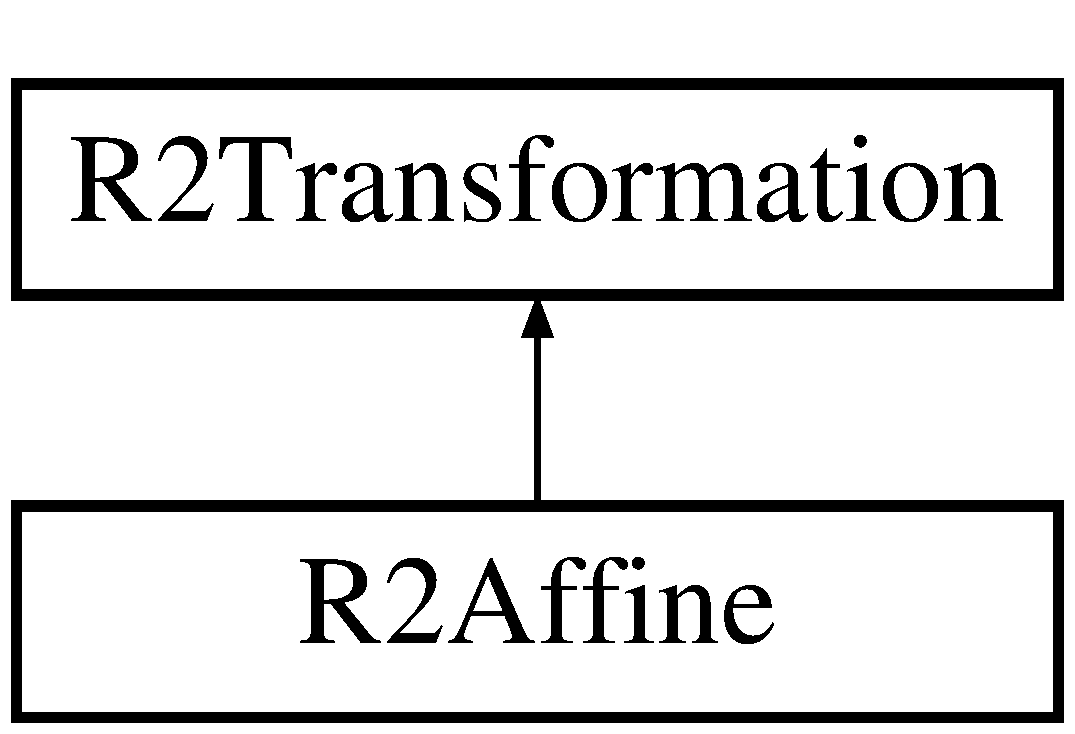
\includegraphics[height=2.000000cm]{class_r2_affine}
\end{center}
\end{figure}
\subsection*{Public Member Functions}
\begin{DoxyCompactItemize}
\item 
{\bfseries R2\+Affine} (const \hyperlink{class_r3_matrix}{R3\+Matrix} \&matrix, R\+N\+Boolean mirror=0)\hypertarget{class_r2_affine_afbf6c50a11cb1fae9e9ee5cc3652d8dc}{}\label{class_r2_affine_afbf6c50a11cb1fae9e9ee5cc3652d8dc}

\item 
const \hyperlink{class_r3_matrix}{R3\+Matrix} \& {\bfseries Matrix} (void) const \hypertarget{class_r2_affine_ae8934f2dbaff8df4f9cfd64d5e12e2b9}{}\label{class_r2_affine_ae8934f2dbaff8df4f9cfd64d5e12e2b9}

\item 
const \hyperlink{class_r3_matrix}{R3\+Matrix} {\bfseries Inverse\+Matrix} (void) const \hypertarget{class_r2_affine_ab81f2dd63c4b1cf320dbfa795156d4ec}{}\label{class_r2_affine_ab81f2dd63c4b1cf320dbfa795156d4ec}

\item 
const R\+N\+Boolean {\bfseries Is\+Mirrored} (void) const \hypertarget{class_r2_affine_a9299c3d3aee30abca64615b2f00b20e8}{}\label{class_r2_affine_a9299c3d3aee30abca64615b2f00b20e8}

\item 
const R\+N\+Boolean {\bfseries Is\+Affine} (void) const \hypertarget{class_r2_affine_a4a3cd8795d3476823b91fe831bfcde9c}{}\label{class_r2_affine_a4a3cd8795d3476823b91fe831bfcde9c}

\item 
const R\+N\+Boolean {\bfseries Is\+Isotropic} (void) const \hypertarget{class_r2_affine_a1af45ac81d41147665302bca14709ef7}{}\label{class_r2_affine_a1af45ac81d41147665302bca14709ef7}

\item 
const R\+N\+Boolean {\bfseries Has\+Translation} (void) const \hypertarget{class_r2_affine_a0e7fd172a538348efff4723d871b940d}{}\label{class_r2_affine_a0e7fd172a538348efff4723d871b940d}

\item 
const R\+N\+Boolean {\bfseries Has\+Scale} (void) const \hypertarget{class_r2_affine_ae06342108d6e677f85f7383f5b9dbfe1}{}\label{class_r2_affine_ae06342108d6e677f85f7383f5b9dbfe1}

\item 
const R\+N\+Boolean {\bfseries Has\+Rotation} (void) const \hypertarget{class_r2_affine_aa1976a92645fd787afac2729ac07f80e}{}\label{class_r2_affine_aa1976a92645fd787afac2729ac07f80e}

\item 
const R\+N\+Boolean {\bfseries Has\+Mirror} (void) const \hypertarget{class_r2_affine_ae3fc6b83f474115c6fb194e620d48cf1}{}\label{class_r2_affine_ae3fc6b83f474115c6fb194e620d48cf1}

\item 
const \hyperlink{class_r2_affine}{R2\+Affine} {\bfseries Inverse} (void) const \hypertarget{class_r2_affine_a1ecb5db09accfc021951507fa8bc71c3}{}\label{class_r2_affine_a1ecb5db09accfc021951507fa8bc71c3}

\item 
const R\+N\+Boolean {\bfseries operator==} (const \hyperlink{class_r2_affine}{R2\+Affine} \&affine) const \hypertarget{class_r2_affine_ab912bab9a532e77a7adc31ca45b4ba5b}{}\label{class_r2_affine_ab912bab9a532e77a7adc31ca45b4ba5b}

\item 
const R\+N\+Boolean {\bfseries operator!=} (const \hyperlink{class_r2_affine}{R2\+Affine} \&affine) const \hypertarget{class_r2_affine_a9f5da2debf8d530d9cc84cf8346d7dbc}{}\label{class_r2_affine_a9f5da2debf8d530d9cc84cf8346d7dbc}

\item 
virtual void {\bfseries Apply} (\hyperlink{class_r2_vector}{R2\+Vector} \&vector) const \hypertarget{class_r2_affine_ae88be855940a4ee7c8570af96e6231a3}{}\label{class_r2_affine_ae88be855940a4ee7c8570af96e6231a3}

\item 
virtual void {\bfseries Apply} (\hyperlink{class_r2_point}{R2\+Point} \&point) const \hypertarget{class_r2_affine_a824715490a1e4c25e8de7e5e7febcea1}{}\label{class_r2_affine_a824715490a1e4c25e8de7e5e7febcea1}

\item 
virtual void {\bfseries Apply} (\hyperlink{class_r2_transformation}{R2\+Transformation} \&transformation) const \hypertarget{class_r2_affine_ac4f92a179bfeb1ccc70666ca613ea69e}{}\label{class_r2_affine_ac4f92a179bfeb1ccc70666ca613ea69e}

\item 
virtual void {\bfseries Apply} (\hyperlink{class_r2_affine}{R2\+Affine} \&affine) const \hypertarget{class_r2_affine_a67c5f12bc5ef56cf38706c9777b3b0cd}{}\label{class_r2_affine_a67c5f12bc5ef56cf38706c9777b3b0cd}

\item 
virtual void {\bfseries Apply\+Inverse} (\hyperlink{class_r2_vector}{R2\+Vector} \&vector) const \hypertarget{class_r2_affine_a85eb1d63c7bc8b5a1dd95ec880099a73}{}\label{class_r2_affine_a85eb1d63c7bc8b5a1dd95ec880099a73}

\item 
virtual void {\bfseries Apply\+Inverse} (\hyperlink{class_r2_point}{R2\+Point} \&point) const \hypertarget{class_r2_affine_a9c61614306572f4b48ccc26b677596e2}{}\label{class_r2_affine_a9c61614306572f4b48ccc26b677596e2}

\item 
virtual void {\bfseries Apply\+Inverse} (\hyperlink{class_r2_transformation}{R2\+Transformation} \&transformation) const \hypertarget{class_r2_affine_a5f8021caca86ddd9034ed7bedd89b2cd}{}\label{class_r2_affine_a5f8021caca86ddd9034ed7bedd89b2cd}

\item 
virtual void {\bfseries Apply\+Inverse} (\hyperlink{class_r2_affine}{R2\+Affine} \&affine) const \hypertarget{class_r2_affine_a06d1c85e5a4177c2827d79eda52df5ee}{}\label{class_r2_affine_a06d1c85e5a4177c2827d79eda52df5ee}

\item 
void {\bfseries Invert} (void)\hypertarget{class_r2_affine_a1c959561b4bc706af845eb8b6f4698e3}{}\label{class_r2_affine_a1c959561b4bc706af845eb8b6f4698e3}

\item 
void {\bfseries X\+Mirror} (void)\hypertarget{class_r2_affine_afc27d2ee78fe58acabd5ac058f037d65}{}\label{class_r2_affine_afc27d2ee78fe58acabd5ac058f037d65}

\item 
void {\bfseries Y\+Mirror} (void)\hypertarget{class_r2_affine_a6b501f99a429ec69b810a51aabc83192}{}\label{class_r2_affine_a6b501f99a429ec69b810a51aabc83192}

\item 
void {\bfseries Mirror} (void)\hypertarget{class_r2_affine_a0e879272c3e6a66b9697a5fa0c9fc7bf}{}\label{class_r2_affine_a0e879272c3e6a66b9697a5fa0c9fc7bf}

\item 
void {\bfseries X\+Translate} (R\+N\+Scalar offset)\hypertarget{class_r2_affine_ae1fdddcd927c8060e9304df4aebfec5a}{}\label{class_r2_affine_ae1fdddcd927c8060e9304df4aebfec5a}

\item 
void {\bfseries Y\+Translate} (R\+N\+Scalar offset)\hypertarget{class_r2_affine_af2d90c14c26e4aa4fbdb957e9ff587e5}{}\label{class_r2_affine_af2d90c14c26e4aa4fbdb957e9ff587e5}

\item 
void {\bfseries Translate} (R\+N\+Scalar offset)\hypertarget{class_r2_affine_a260110e1dc7228b0b9b2b5589c1a85b6}{}\label{class_r2_affine_a260110e1dc7228b0b9b2b5589c1a85b6}

\item 
void {\bfseries Translate} (R\+N\+Axis axis, R\+N\+Scalar offset)\hypertarget{class_r2_affine_a7beb5fd439b6d0effb5acac80bfcc8df}{}\label{class_r2_affine_a7beb5fd439b6d0effb5acac80bfcc8df}

\item 
void {\bfseries Translate} (const \hyperlink{class_r2_vector}{R2\+Vector} \&offset)\hypertarget{class_r2_affine_a689090e063e450da204aa3e6dc41e2cd}{}\label{class_r2_affine_a689090e063e450da204aa3e6dc41e2cd}

\item 
void {\bfseries X\+Scale} (R\+N\+Scalar scale)\hypertarget{class_r2_affine_a9f3886954ae9f0129be639b7b1906140}{}\label{class_r2_affine_a9f3886954ae9f0129be639b7b1906140}

\item 
void {\bfseries Y\+Scale} (R\+N\+Scalar scale)\hypertarget{class_r2_affine_a0d45f20d91b865d0af4c0efcc33d43ac}{}\label{class_r2_affine_a0d45f20d91b865d0af4c0efcc33d43ac}

\item 
void {\bfseries Scale} (R\+N\+Scalar scale)\hypertarget{class_r2_affine_a958c4f2955f734b5aece7b96694bf394}{}\label{class_r2_affine_a958c4f2955f734b5aece7b96694bf394}

\item 
void {\bfseries Scale} (R\+N\+Axis axis, R\+N\+Scalar scale)\hypertarget{class_r2_affine_a64a6f469fa92c4d38e65fd7f09475a80}{}\label{class_r2_affine_a64a6f469fa92c4d38e65fd7f09475a80}

\item 
void {\bfseries Scale} (const \hyperlink{class_r2_vector}{R2\+Vector} \&scale)\hypertarget{class_r2_affine_ae18b7a8a7ca203d4dbfe940c0c704833}{}\label{class_r2_affine_ae18b7a8a7ca203d4dbfe940c0c704833}

\item 
void {\bfseries Rotate} (R\+N\+Angle radians)\hypertarget{class_r2_affine_a667d5c45bcf9fe1a8b31c4aecf5ed929}{}\label{class_r2_affine_a667d5c45bcf9fe1a8b31c4aecf5ed929}

\item 
void {\bfseries Transform} (const \hyperlink{class_r2_transformation}{R2\+Transformation} \&transformation)\hypertarget{class_r2_affine_adfc10a572683a580a460f0e1b0072d82}{}\label{class_r2_affine_adfc10a572683a580a460f0e1b0072d82}

\item 
void {\bfseries Transform} (const \hyperlink{class_r2_affine}{R2\+Affine} \&affine)\hypertarget{class_r2_affine_a43899898abe9d4d95cd895decdc55495}{}\label{class_r2_affine_a43899898abe9d4d95cd895decdc55495}

\item 
void {\bfseries Inverse\+Transform} (const \hyperlink{class_r2_transformation}{R2\+Transformation} \&transformation)\hypertarget{class_r2_affine_a85e30d8df0dd0a1c7b9971cc0bed2e59}{}\label{class_r2_affine_a85e30d8df0dd0a1c7b9971cc0bed2e59}

\item 
void {\bfseries Inverse\+Transform} (const \hyperlink{class_r2_affine}{R2\+Affine} \&affine)\hypertarget{class_r2_affine_ae94abc9cbe6875f452e3f604aa95d8af}{}\label{class_r2_affine_ae94abc9cbe6875f452e3f604aa95d8af}

\item 
void {\bfseries Reset} (const \hyperlink{class_r2_transformation}{R2\+Transformation} \&transformation)\hypertarget{class_r2_affine_ac1efebf9997cc0b74d0c81ce71532d95}{}\label{class_r2_affine_ac1efebf9997cc0b74d0c81ce71532d95}

\item 
void {\bfseries Reset} (const \hyperlink{class_r3_matrix}{R3\+Matrix} \&matrix, R\+N\+Boolean mirror=0)\hypertarget{class_r2_affine_a921a4e00c19cb12a03cf68f10f59b4a5}{}\label{class_r2_affine_a921a4e00c19cb12a03cf68f10f59b4a5}

\item 
virtual void {\bfseries Load} (void) const \hypertarget{class_r2_affine_a19432114bc764f7e8f5d1760c4d64086}{}\label{class_r2_affine_a19432114bc764f7e8f5d1760c4d64086}

\item 
virtual void {\bfseries Draw} (void) const \hypertarget{class_r2_affine_a04ed63532964524b986fbdc3a1e94c48}{}\label{class_r2_affine_a04ed63532964524b986fbdc3a1e94c48}

\item 
virtual void {\bfseries Push} (void) const \hypertarget{class_r2_affine_ad3125cf5dd10887394ab1efdacc3028c}{}\label{class_r2_affine_ad3125cf5dd10887394ab1efdacc3028c}

\item 
virtual void {\bfseries Pop} (void) const \hypertarget{class_r2_affine_adcf72df4a772d2fa94065252af9c76d3}{}\label{class_r2_affine_adcf72df4a772d2fa94065252af9c76d3}

\item 
const R\+N\+Scalar {\bfseries Scale\+Factor} (void) const \hypertarget{class_r2_affine_af76ac8f0f85c269630fa577f33466bbb}{}\label{class_r2_affine_af76ac8f0f85c269630fa577f33466bbb}

\end{DoxyCompactItemize}


The documentation for this class was generated from the following files\+:\begin{DoxyCompactItemize}
\item 
R2\+Shapes/R2\+Affine.\+h\item 
R2\+Shapes/R2\+Affine.\+cpp\item 
R2\+Shapes/R2\+Draw.\+cpp\end{DoxyCompactItemize}

\hypertarget{class_r2_arc}{}\section{R2\+Arc Class Reference}
\label{class_r2_arc}\index{R2\+Arc@{R2\+Arc}}
Inheritance diagram for R2\+Arc\+:\begin{figure}[H]
\begin{center}
\leavevmode
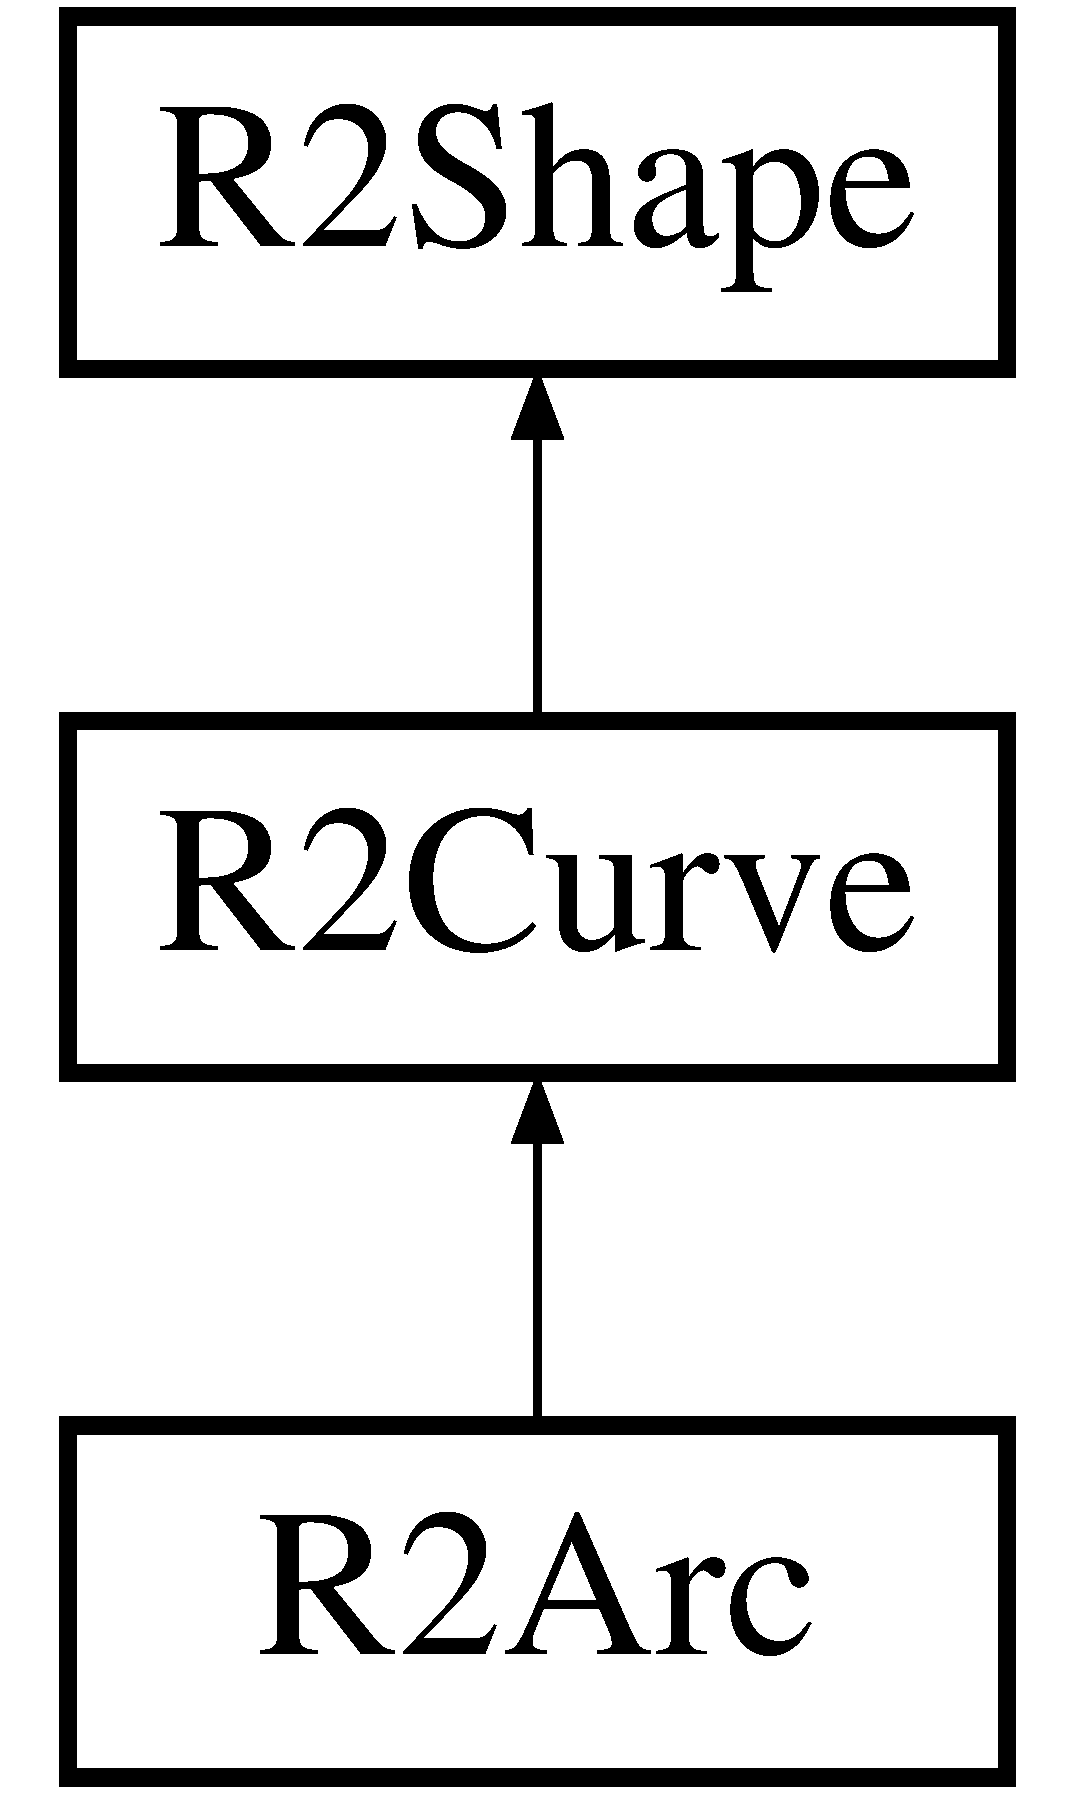
\includegraphics[height=3.000000cm]{class_r2_arc}
\end{center}
\end{figure}
\subsection*{Public Member Functions}
\begin{DoxyCompactItemize}
\item 
{\bfseries R2\+Arc} (const \hyperlink{class_r2_arc}{R2\+Arc} \&arc)\hypertarget{class_r2_arc_ae96f4dd17baf62785b2659e6a0973656}{}\label{class_r2_arc_ae96f4dd17baf62785b2659e6a0973656}

\item 
{\bfseries R2\+Arc} (const \hyperlink{class_r2_point}{R2\+Point} \&center, R\+N\+Length radius, R\+N\+Angle start, R\+N\+Angle stop)\hypertarget{class_r2_arc_aca58ac277d17dfa4b82a5a70e26defa7}{}\label{class_r2_arc_aca58ac277d17dfa4b82a5a70e26defa7}

\item 
const \hyperlink{class_r2_circle}{R2\+Circle} \& {\bfseries Circle} (void) const \hypertarget{class_r2_arc_a60fd02d6bd30e28f785a0e57d17dfd13}{}\label{class_r2_arc_a60fd02d6bd30e28f785a0e57d17dfd13}

\item 
const \hyperlink{class_r2_point}{R2\+Point} \& {\bfseries Center} (void) const \hypertarget{class_r2_arc_a76b04ddff70277a7b8b319c65251a159}{}\label{class_r2_arc_a76b04ddff70277a7b8b319c65251a159}

\item 
const R\+N\+Length {\bfseries Radius} (void) const \hypertarget{class_r2_arc_abb69ecedff2225f1812f0e1d51c63001}{}\label{class_r2_arc_abb69ecedff2225f1812f0e1d51c63001}

\item 
const R\+N\+Angle {\bfseries Start\+Angle} (void) const \hypertarget{class_r2_arc_a87ed1499c75cfeebe319fe54fd88c24d}{}\label{class_r2_arc_a87ed1499c75cfeebe319fe54fd88c24d}

\item 
const R\+N\+Angle {\bfseries Stop\+Angle} (void) const \hypertarget{class_r2_arc_a063b194c0799c458ec1fe739c8cebb2b}{}\label{class_r2_arc_a063b194c0799c458ec1fe739c8cebb2b}

\item 
const R\+N\+Angle {\bfseries Sweep\+Angle} (void) const \hypertarget{class_r2_arc_a36185350c5f5c4ab1b56c9c648f1159e}{}\label{class_r2_arc_a36185350c5f5c4ab1b56c9c648f1159e}

\item 
const \hyperlink{class_r2_point}{R2\+Point} {\bfseries Point} (R\+N\+Angle angle) const \hypertarget{class_r2_arc_a7f2ab3ff07b0554380a2a6a113ccbf1d}{}\label{class_r2_arc_a7f2ab3ff07b0554380a2a6a113ccbf1d}

\item 
const \hyperlink{class_r2_point}{R2\+Point} {\bfseries Mid\+Point} (void) const \hypertarget{class_r2_arc_ab12a76c4beab47fd53d1dd6367b26fed}{}\label{class_r2_arc_ab12a76c4beab47fd53d1dd6367b26fed}

\item 
const \hyperlink{class_r2_point}{R2\+Point} {\bfseries Start\+Point} (void) const \hypertarget{class_r2_arc_aad9f4b2a7e11ce3f7726cb7f18699978}{}\label{class_r2_arc_aad9f4b2a7e11ce3f7726cb7f18699978}

\item 
const \hyperlink{class_r2_point}{R2\+Point} {\bfseries Stop\+Point} (void) const \hypertarget{class_r2_arc_aab29f137c725113f256e92b4941488f9}{}\label{class_r2_arc_aab29f137c725113f256e92b4941488f9}

\item 
const R\+N\+Boolean {\bfseries Is\+Empty} (void) const \hypertarget{class_r2_arc_a3da24ee22d9e7a6129c42d1427d6cba0}{}\label{class_r2_arc_a3da24ee22d9e7a6129c42d1427d6cba0}

\item 
const R\+N\+Boolean {\bfseries Is\+Finite} (void) const \hypertarget{class_r2_arc_a37c4dea73b42146f5fdf4f85db5bc07b}{}\label{class_r2_arc_a37c4dea73b42146f5fdf4f85db5bc07b}

\item 
virtual const R\+N\+Boolean {\bfseries Is\+Point} (void) const \hypertarget{class_r2_arc_ad8d6a4add1021a21aa60b9f6d38108d5}{}\label{class_r2_arc_ad8d6a4add1021a21aa60b9f6d38108d5}

\item 
virtual const R\+N\+Boolean {\bfseries Is\+Linear} (void) const \hypertarget{class_r2_arc_a45b4b16e4a81d96a545bff759a7e0201}{}\label{class_r2_arc_a45b4b16e4a81d96a545bff759a7e0201}

\item 
virtual const R\+N\+Boolean {\bfseries Is\+Convex} (void) const \hypertarget{class_r2_arc_afede8d69b10718c2705d83d91047e951}{}\label{class_r2_arc_afede8d69b10718c2705d83d91047e951}

\item 
virtual const \hyperlink{class_r2_point}{R2\+Point} {\bfseries Centroid} (void) const \hypertarget{class_r2_arc_aa6e707f840f9fe64a2efc18a2736f8c8}{}\label{class_r2_arc_aa6e707f840f9fe64a2efc18a2736f8c8}

\item 
virtual const \hyperlink{class_r2_shape}{R2\+Shape} \& {\bfseries B\+Shape} (void) const \hypertarget{class_r2_arc_abe97b60bd09de5a35e1ce5f49f4a7d6f}{}\label{class_r2_arc_abe97b60bd09de5a35e1ce5f49f4a7d6f}

\item 
virtual const \hyperlink{class_r2_box}{R2\+Box} {\bfseries B\+Box} (void) const \hypertarget{class_r2_arc_a330e00729b7986c609751338576ba8ea}{}\label{class_r2_arc_a330e00729b7986c609751338576ba8ea}

\item 
virtual const \hyperlink{class_r2_circle}{R2\+Circle} {\bfseries B\+Circle} (void) const \hypertarget{class_r2_arc_a18450649651040aa4eb125f6ab7a4171}{}\label{class_r2_arc_a18450649651040aa4eb125f6ab7a4171}

\item 
virtual void {\bfseries Empty} (void)\hypertarget{class_r2_arc_a6dca2ff474041fc577195408a5c576e9}{}\label{class_r2_arc_a6dca2ff474041fc577195408a5c576e9}

\item 
virtual void {\bfseries Set\+Start\+Angle} (R\+N\+Angle theta)\hypertarget{class_r2_arc_a03a88e8c029e26d72c1df2e52b9b0e91}{}\label{class_r2_arc_a03a88e8c029e26d72c1df2e52b9b0e91}

\item 
virtual void {\bfseries Set\+Stop\+Angle} (R\+N\+Angle theta)\hypertarget{class_r2_arc_abdcef205613cc05a84f7fb1475fc9381}{}\label{class_r2_arc_abdcef205613cc05a84f7fb1475fc9381}

\item 
virtual void {\bfseries Translate} (const \hyperlink{class_r2_vector}{R2\+Vector} \&vector)\hypertarget{class_r2_arc_a72ae89551a111a2bde6f81e4f9fa092a}{}\label{class_r2_arc_a72ae89551a111a2bde6f81e4f9fa092a}

\item 
virtual void {\bfseries Reposition} (const \hyperlink{class_r2_point}{R2\+Point} \&center)\hypertarget{class_r2_arc_ade95d2c9283d5d180bfa4d640aa082f8}{}\label{class_r2_arc_ade95d2c9283d5d180bfa4d640aa082f8}

\item 
virtual void {\bfseries Resize} (R\+N\+Length radius)\hypertarget{class_r2_arc_a13b4a2d7f1805515f072ba28b530d7ae}{}\label{class_r2_arc_a13b4a2d7f1805515f072ba28b530d7ae}

\item 
virtual void {\bfseries Transform} (const \hyperlink{class_r2_transformation}{R2\+Transformation} \&transformation)\hypertarget{class_r2_arc_aefb2550eb245b6990a93babdcab01ad2}{}\label{class_r2_arc_aefb2550eb245b6990a93babdcab01ad2}

\item 
virtual void {\bfseries Draw} (const \hyperlink{class_r_n_flags}{R2\+Draw\+Flags} draw\+\_\+flags=R2\+\_\+\+D\+E\+F\+A\+U\+L\+T\+\_\+\+D\+R\+A\+W\+\_\+\+F\+L\+A\+GS) const \hypertarget{class_r2_arc_af2059271304ead9264f2546890a986b3}{}\label{class_r2_arc_af2059271304ead9264f2546890a986b3}

\end{DoxyCompactItemize}


The documentation for this class was generated from the following files\+:\begin{DoxyCompactItemize}
\item 
R2\+Shapes/R2\+Arc.\+h\item 
R2\+Shapes/R2\+Arc.\+cpp\item 
R2\+Shapes/R2\+Draw.\+cpp\end{DoxyCompactItemize}

\hypertarget{class_r2_box}{}\section{R2\+Box Class Reference}
\label{class_r2_box}\index{R2\+Box@{R2\+Box}}
Inheritance diagram for R2\+Box\+:\begin{figure}[H]
\begin{center}
\leavevmode
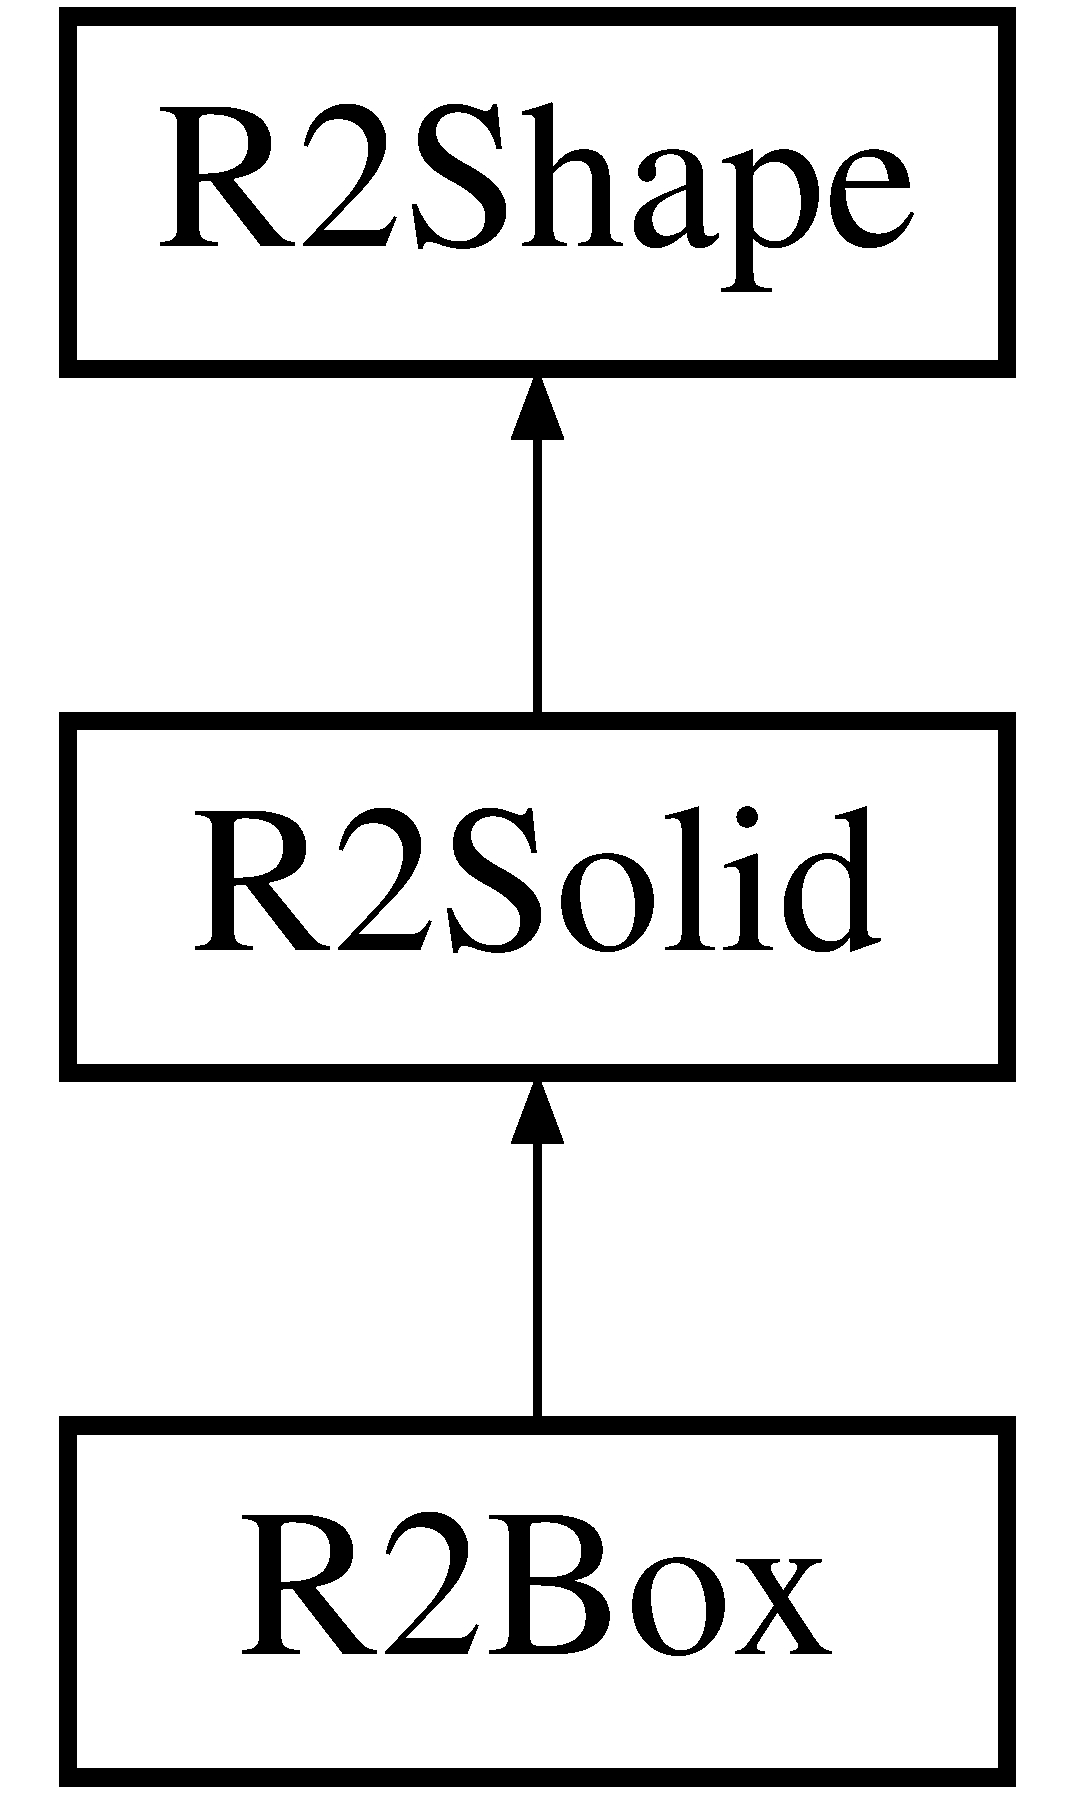
\includegraphics[height=3.000000cm]{class_r2_box}
\end{center}
\end{figure}
\subsection*{Public Member Functions}
\begin{DoxyCompactItemize}
\item 
{\bfseries R2\+Box} (const \hyperlink{class_r2_box}{R2\+Box} \&\hyperlink{structbox}{box})\hypertarget{class_r2_box_a127e292224b01bcdce432230427a939a}{}\label{class_r2_box_a127e292224b01bcdce432230427a939a}

\item 
{\bfseries R2\+Box} (const \hyperlink{class_r2_point}{R2\+Point} \&min, const \hyperlink{class_r2_point}{R2\+Point} \&max)\hypertarget{class_r2_box_a83ae8c3cf4ee60fbb8fd9d979306aa6d}{}\label{class_r2_box_a83ae8c3cf4ee60fbb8fd9d979306aa6d}

\item 
{\bfseries R2\+Box} (const \hyperlink{class_r2_point}{R2\+Point} \&center, R\+N\+Length xradius, R\+N\+Length yradius)\hypertarget{class_r2_box_a3247ae91adcdfe432af88259093d426c}{}\label{class_r2_box_a3247ae91adcdfe432af88259093d426c}

\item 
{\bfseries R2\+Box} (R\+N\+Coord xmin, R\+N\+Coord ymin, R\+N\+Coord xmax, R\+N\+Coord ymax)\hypertarget{class_r2_box_a13d265b1f0d15d03edd856f89e083f3d}{}\label{class_r2_box_a13d265b1f0d15d03edd856f89e083f3d}

\item 
const R\+N\+Coord {\bfseries X\+Min} (void) const \hypertarget{class_r2_box_a82145070f2927859a1e5b8f25ce38094}{}\label{class_r2_box_a82145070f2927859a1e5b8f25ce38094}

\item 
const R\+N\+Coord {\bfseries Y\+Min} (void) const \hypertarget{class_r2_box_a8b9fec16e044ca636cba917dccf220c3}{}\label{class_r2_box_a8b9fec16e044ca636cba917dccf220c3}

\item 
const R\+N\+Coord {\bfseries X\+Max} (void) const \hypertarget{class_r2_box_af6dc0f420575381df0e3bc3a252200a6}{}\label{class_r2_box_af6dc0f420575381df0e3bc3a252200a6}

\item 
const R\+N\+Coord {\bfseries Y\+Max} (void) const \hypertarget{class_r2_box_a9d3a78db8f32542628656cbe2e16e1a8}{}\label{class_r2_box_a9d3a78db8f32542628656cbe2e16e1a8}

\item 
const R\+N\+Coord {\bfseries Coord} (R\+N\+Direction dir, R\+N\+Dimension dim) const \hypertarget{class_r2_box_a3a8b91e5e0c3ee943a9948dfafb56215}{}\label{class_r2_box_a3a8b91e5e0c3ee943a9948dfafb56215}

\item 
const \hyperlink{class_r2_point}{R2\+Point} \& {\bfseries Min} (void) const \hypertarget{class_r2_box_adf65e166cef0b308be655c93dc6cbcdf}{}\label{class_r2_box_adf65e166cef0b308be655c93dc6cbcdf}

\item 
const \hyperlink{class_r2_point}{R2\+Point} \& {\bfseries Max} (void) const \hypertarget{class_r2_box_a8a815031a0e0945134d6860bc99ac411}{}\label{class_r2_box_a8a815031a0e0945134d6860bc99ac411}

\item 
const \hyperlink{class_r2_point}{R2\+Point} {\bfseries Corner} (R\+N\+Quadrant quadrant) const \hypertarget{class_r2_box_a8ca9227724e7174282f7e69d0b2d39c2}{}\label{class_r2_box_a8ca9227724e7174282f7e69d0b2d39c2}

\item 
const \hyperlink{class_r2_point}{R2\+Point} {\bfseries Corner} (R\+N\+Direction xdir, R\+N\+Direction ydir) const \hypertarget{class_r2_box_a67ab8c1e3f3376ae1d4a15ab1b7f621b}{}\label{class_r2_box_a67ab8c1e3f3376ae1d4a15ab1b7f621b}

\item 
const \hyperlink{class_r2_point}{R2\+Point} {\bfseries Centroid} (void) const \hypertarget{class_r2_box_a78831c39aa836c228bced6c50233f19c}{}\label{class_r2_box_a78831c39aa836c228bced6c50233f19c}

\item 
const \hyperlink{class_r2_point}{R2\+Point} {\bfseries Closest\+Point} (const \hyperlink{class_r2_point}{R2\+Point} \&point) const \hypertarget{class_r2_box_acacf37f0f104fc67a2df2596daacd53a}{}\label{class_r2_box_acacf37f0f104fc67a2df2596daacd53a}

\item 
const \hyperlink{class_r2_box}{R2\+Box} {\bfseries Quadrant} (R\+N\+Quadrant octant) const \hypertarget{class_r2_box_a2786f7110cc993e1af6fdb8ca4e4bc7c}{}\label{class_r2_box_a2786f7110cc993e1af6fdb8ca4e4bc7c}

\item 
const \hyperlink{class_r2_box}{R2\+Box} {\bfseries Quadrant} (R\+N\+Direction xdir, R\+N\+Direction ydir) const \hypertarget{class_r2_box_a19f1e394e6aefe2cd6057298a5f9bfea}{}\label{class_r2_box_a19f1e394e6aefe2cd6057298a5f9bfea}

\item 
const R\+N\+Boolean {\bfseries Is\+Empty} (void) const \hypertarget{class_r2_box_ab5f8331a43680ef57fd3eb09f8b46dfa}{}\label{class_r2_box_ab5f8331a43680ef57fd3eb09f8b46dfa}

\item 
const R\+N\+Boolean {\bfseries Is\+Finite} (void) const \hypertarget{class_r2_box_a62d577bdf9766fbe8b48d81b080a385f}{}\label{class_r2_box_a62d577bdf9766fbe8b48d81b080a385f}

\item 
const int {\bfseries N\+Dimensions} (void) const \hypertarget{class_r2_box_af1b950d7ad219912f013888099c3f1e1}{}\label{class_r2_box_af1b950d7ad219912f013888099c3f1e1}

\item 
const R\+N\+Boolean {\bfseries Is\+Axis\+Null} (const R\+N\+Axis axis) const \hypertarget{class_r2_box_a7a7fb7e1e1ec7a4054d6977e0ab7bd24}{}\label{class_r2_box_a7a7fb7e1e1ec7a4054d6977e0ab7bd24}

\item 
const R\+N\+Length {\bfseries X\+Length} (void) const \hypertarget{class_r2_box_a7799dee779e65e05d8706268fdd781b9}{}\label{class_r2_box_a7799dee779e65e05d8706268fdd781b9}

\item 
const R\+N\+Length {\bfseries Y\+Length} (void) const \hypertarget{class_r2_box_a2a11fc13e01af6e3406e786c6fac2a80}{}\label{class_r2_box_a2a11fc13e01af6e3406e786c6fac2a80}

\item 
const R\+N\+Length {\bfseries Axis\+Length} (const R\+N\+Axis axis) const \hypertarget{class_r2_box_a1c6d4035f6233b3e28d4c58ca1c116fd}{}\label{class_r2_box_a1c6d4035f6233b3e28d4c58ca1c116fd}

\item 
const R\+N\+Length {\bfseries Diagonal\+Length} (void) const \hypertarget{class_r2_box_a3710743c6019ae501cb21cfc112c8d12}{}\label{class_r2_box_a3710743c6019ae501cb21cfc112c8d12}

\item 
const R\+N\+Length {\bfseries X\+Radius} (void) const \hypertarget{class_r2_box_a2d169bc15a9522100f7f408714d342b8}{}\label{class_r2_box_a2d169bc15a9522100f7f408714d342b8}

\item 
const R\+N\+Length {\bfseries Y\+Radius} (void) const \hypertarget{class_r2_box_a9a0f3b70398d507cd44d31b0d01cb135}{}\label{class_r2_box_a9a0f3b70398d507cd44d31b0d01cb135}

\item 
const R\+N\+Length {\bfseries Axis\+Radius} (const R\+N\+Axis axis) const \hypertarget{class_r2_box_a61766b6503d244fa1121985c04126b45}{}\label{class_r2_box_a61766b6503d244fa1121985c04126b45}

\item 
const R\+N\+Length {\bfseries Diagonal\+Radius} (void) const \hypertarget{class_r2_box_a00ab031acf3086b5c738e409072628b9}{}\label{class_r2_box_a00ab031acf3086b5c738e409072628b9}

\item 
const R\+N\+Coord {\bfseries X\+Center} (void) const \hypertarget{class_r2_box_a4d7137a8b33d25073488f9beb6fee01b}{}\label{class_r2_box_a4d7137a8b33d25073488f9beb6fee01b}

\item 
const R\+N\+Coord {\bfseries Y\+Center} (void) const \hypertarget{class_r2_box_ad5a3bbf14b4905e364ad04a305c669aa}{}\label{class_r2_box_ad5a3bbf14b4905e364ad04a305c669aa}

\item 
const R\+N\+Coord {\bfseries Axis\+Center} (const R\+N\+Axis axis) const \hypertarget{class_r2_box_af3af7a7848270df64621b09bf4678ad0}{}\label{class_r2_box_af3af7a7848270df64621b09bf4678ad0}

\item 
const R\+N\+Axis {\bfseries Shortest\+Axis} (void) const \hypertarget{class_r2_box_a7168b00e526e0881910495d3335b5f9f}{}\label{class_r2_box_a7168b00e526e0881910495d3335b5f9f}

\item 
const R\+N\+Axis {\bfseries Longest\+Axis} (void) const \hypertarget{class_r2_box_a65ba59f99e319f658d460b3fd3f9807e}{}\label{class_r2_box_a65ba59f99e319f658d460b3fd3f9807e}

\item 
const R\+N\+Length {\bfseries Shortest\+Axis\+Length} (void) const \hypertarget{class_r2_box_adf1422c1522ea28a7f7014b531634996}{}\label{class_r2_box_adf1422c1522ea28a7f7014b531634996}

\item 
const R\+N\+Length {\bfseries Longest\+Axis\+Length} (void) const \hypertarget{class_r2_box_ac695d89dd62d9974c661fa8d22a42730}{}\label{class_r2_box_ac695d89dd62d9974c661fa8d22a42730}

\item 
virtual const R\+N\+Boolean {\bfseries Is\+Point} (void) const \hypertarget{class_r2_box_a74202d8d53552e6d2da87f94276e86e9}{}\label{class_r2_box_a74202d8d53552e6d2da87f94276e86e9}

\item 
virtual const R\+N\+Boolean {\bfseries Is\+Linear} (void) const \hypertarget{class_r2_box_a50c23ec05b1714263249c3d025caa1fd}{}\label{class_r2_box_a50c23ec05b1714263249c3d025caa1fd}

\item 
virtual const R\+N\+Boolean {\bfseries Is\+Convex} (void) const \hypertarget{class_r2_box_a6f495ebad69f37e6c5e8b5ef1ca3557b}{}\label{class_r2_box_a6f495ebad69f37e6c5e8b5ef1ca3557b}

\item 
virtual const R\+N\+Area {\bfseries Area} (void) const \hypertarget{class_r2_box_a424bd04630419ed44f1cbe2c3d56b15f}{}\label{class_r2_box_a424bd04630419ed44f1cbe2c3d56b15f}

\item 
virtual const \hyperlink{class_r2_shape}{R2\+Shape} \& {\bfseries B\+Shape} (void) const \hypertarget{class_r2_box_a856e96af2c43771e8fc6fab0a0d08d77}{}\label{class_r2_box_a856e96af2c43771e8fc6fab0a0d08d77}

\item 
virtual const \hyperlink{class_r2_box}{R2\+Box} {\bfseries B\+Box} (void) const \hypertarget{class_r2_box_a3fa3050507c86c4c27840e3abf6c8a04}{}\label{class_r2_box_a3fa3050507c86c4c27840e3abf6c8a04}

\item 
virtual const \hyperlink{class_r2_circle}{R2\+Circle} {\bfseries B\+Circle} (void) const \hypertarget{class_r2_box_a374f79e1fa6e6a6c8e8815281997080a}{}\label{class_r2_box_a374f79e1fa6e6a6c8e8815281997080a}

\item 
virtual void {\bfseries Empty} (void)\hypertarget{class_r2_box_adfa30dd7fb6fa949a04fe3619ba9806e}{}\label{class_r2_box_adfa30dd7fb6fa949a04fe3619ba9806e}

\item 
virtual void {\bfseries Inflate} (R\+N\+Scalar fraction)\hypertarget{class_r2_box_a9fcfbe9cd6ea1f7ffc6b990bf49eb4f5}{}\label{class_r2_box_a9fcfbe9cd6ea1f7ffc6b990bf49eb4f5}

\item 
virtual void {\bfseries Translate} (const \hyperlink{class_r2_vector}{R2\+Vector} \&vector)\hypertarget{class_r2_box_a5c516aba8ccf765494b1374642747660}{}\label{class_r2_box_a5c516aba8ccf765494b1374642747660}

\item 
virtual void {\bfseries Union} (const \hyperlink{class_r2_point}{R2\+Point} \&point)\hypertarget{class_r2_box_aae64766b9d5950e56cade1009838a422}{}\label{class_r2_box_aae64766b9d5950e56cade1009838a422}

\item 
virtual void {\bfseries Union} (const \hyperlink{class_r2_box}{R2\+Box} \&\hyperlink{structbox}{box})\hypertarget{class_r2_box_a7e4cf0e1f9ecbeea6bb31664d3b0ae58}{}\label{class_r2_box_a7e4cf0e1f9ecbeea6bb31664d3b0ae58}

\item 
virtual void {\bfseries Union} (const \hyperlink{class_r2_circle}{R2\+Circle} \&circle)\hypertarget{class_r2_box_aa89b8726525dffebca9e6166cf6a9e85}{}\label{class_r2_box_aa89b8726525dffebca9e6166cf6a9e85}

\item 
virtual void {\bfseries Intersect} (const \hyperlink{class_r2_box}{R2\+Box} \&\hyperlink{structbox}{box})\hypertarget{class_r2_box_aa46530103f9cf387ae0170b8efb86c69}{}\label{class_r2_box_aa46530103f9cf387ae0170b8efb86c69}

\item 
virtual void {\bfseries Transform} (const \hyperlink{class_r2_transformation}{R2\+Transformation} \&transformation)\hypertarget{class_r2_box_a31700b63d98b13a04b009eb6726aa7a3}{}\label{class_r2_box_a31700b63d98b13a04b009eb6726aa7a3}

\item 
virtual void {\bfseries Reset} (const \hyperlink{class_r2_point}{R2\+Point} \&min, const \hyperlink{class_r2_point}{R2\+Point} \&max)\hypertarget{class_r2_box_a5318054136a8153ba490ec24495f4087}{}\label{class_r2_box_a5318054136a8153ba490ec24495f4087}

\item 
virtual void {\bfseries Draw} (const \hyperlink{class_r_n_flags}{R2\+Draw\+Flags} draw\+\_\+flags=R2\+\_\+\+D\+E\+F\+A\+U\+L\+T\+\_\+\+D\+R\+A\+W\+\_\+\+F\+L\+A\+GS) const \hypertarget{class_r2_box_a201085e1320fbdf46f367145b84c05d7}{}\label{class_r2_box_a201085e1320fbdf46f367145b84c05d7}

\item 
R\+N\+Boolean {\bfseries operator==} (const \hyperlink{class_r2_box}{R2\+Box} \&\hyperlink{structbox}{box}) const \hypertarget{class_r2_box_af3f8f5dc797f91bc3eba62eeb1f95245}{}\label{class_r2_box_af3f8f5dc797f91bc3eba62eeb1f95245}

\item 
R\+N\+Boolean {\bfseries operator!=} (const \hyperlink{class_r2_box}{R2\+Box} \&\hyperlink{structbox}{box}) const \hypertarget{class_r2_box_a982d01bbf88244a7aeee0d61f63715c4}{}\label{class_r2_box_a982d01bbf88244a7aeee0d61f63715c4}

\item 
const \hyperlink{class_r2_point}{R2\+Point} \& {\bfseries operator\mbox{[}$\,$\mbox{]}} (R\+N\+Direction dir) const \hypertarget{class_r2_box_acc5a13137a0eb6ffca7a3892737f3073}{}\label{class_r2_box_acc5a13137a0eb6ffca7a3892737f3073}

\item 
\hyperlink{class_r2_point}{R2\+Point} \& {\bfseries operator\mbox{[}$\,$\mbox{]}} (R\+N\+Direction dir)\hypertarget{class_r2_box_acc7598c3fa12dafbb4ee15bc57faf9fc}{}\label{class_r2_box_acc7598c3fa12dafbb4ee15bc57faf9fc}

\end{DoxyCompactItemize}


The documentation for this class was generated from the following files\+:\begin{DoxyCompactItemize}
\item 
R2\+Shapes/R2\+Box.\+h\item 
R2\+Shapes/R2\+Box.\+cpp\item 
R2\+Shapes/R2\+Draw.\+cpp\end{DoxyCompactItemize}

\hypertarget{class_r2_circle}{}\section{R2\+Circle Class Reference}
\label{class_r2_circle}\index{R2\+Circle@{R2\+Circle}}
Inheritance diagram for R2\+Circle\+:\begin{figure}[H]
\begin{center}
\leavevmode
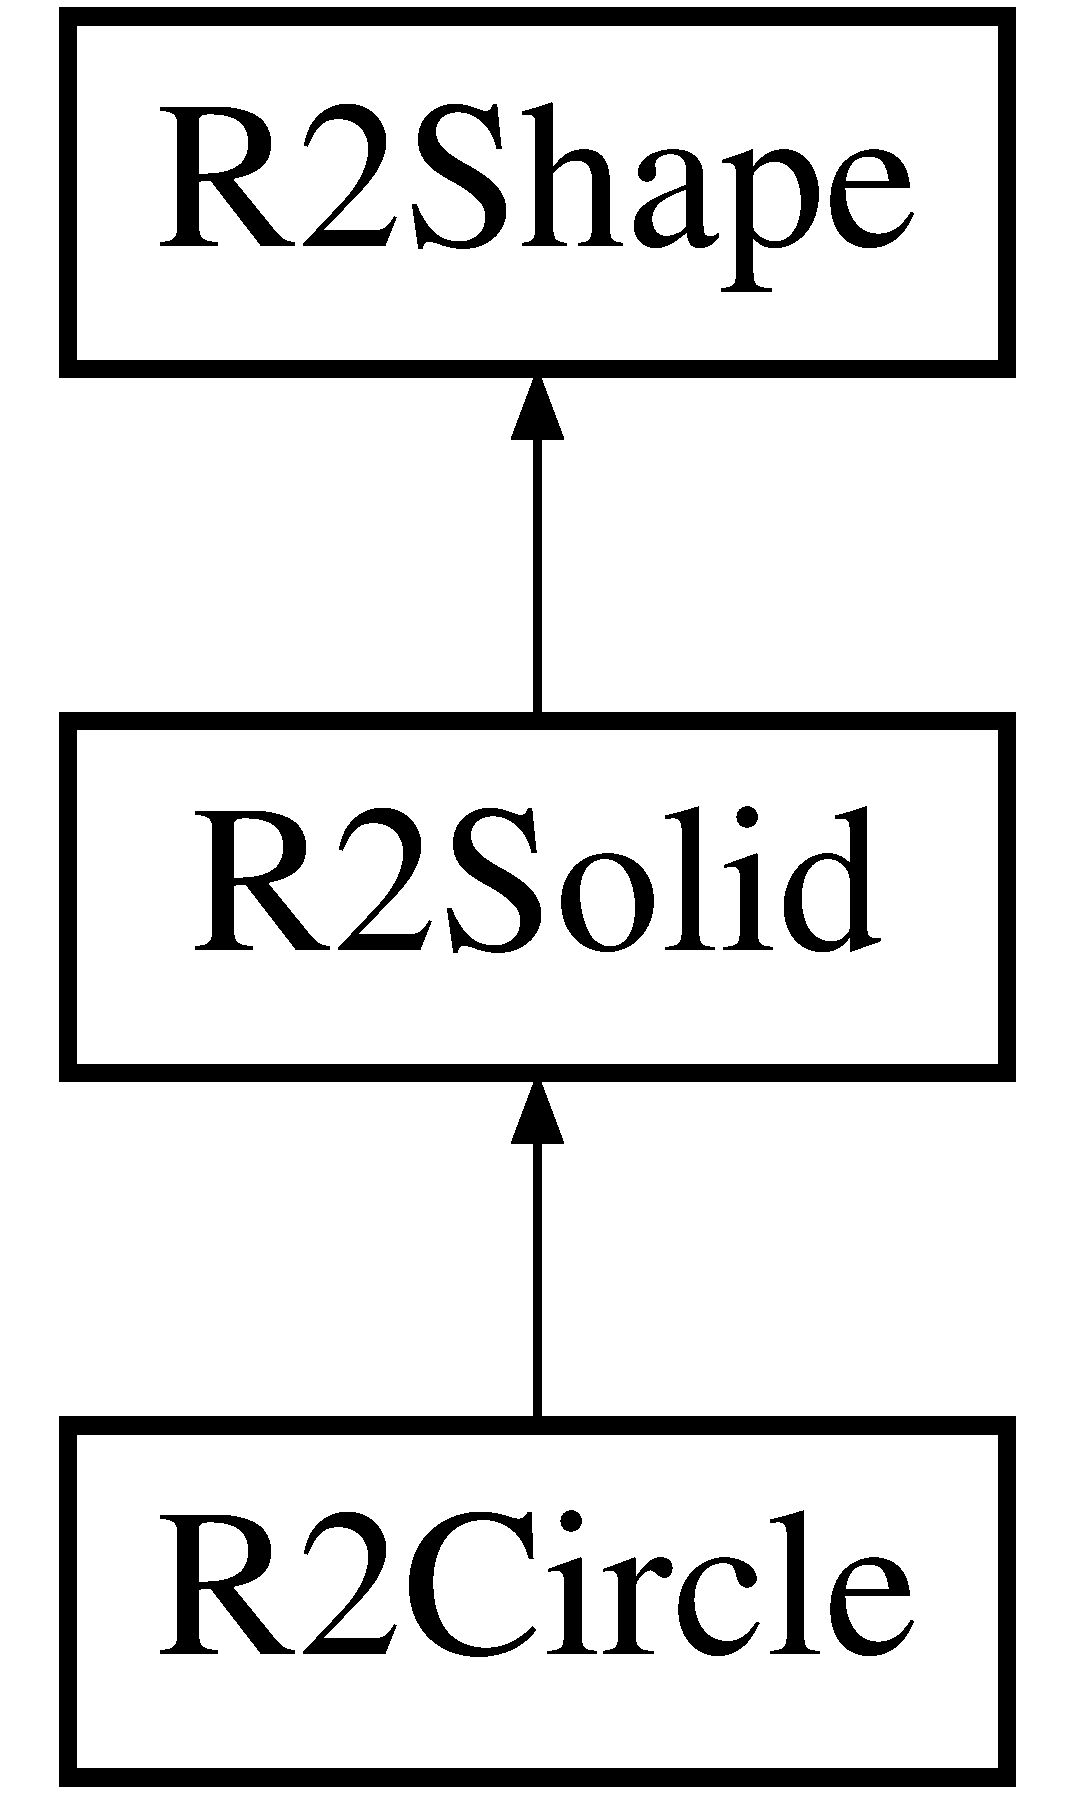
\includegraphics[height=3.000000cm]{class_r2_circle}
\end{center}
\end{figure}
\subsection*{Public Member Functions}
\begin{DoxyCompactItemize}
\item 
{\bfseries R2\+Circle} (const \hyperlink{class_r2_circle}{R2\+Circle} \&circle)\hypertarget{class_r2_circle_aea0db03ef12498517373e3055508ec28}{}\label{class_r2_circle_aea0db03ef12498517373e3055508ec28}

\item 
{\bfseries R2\+Circle} (const \hyperlink{class_r2_point}{R2\+Point} \&center, R\+N\+Length radius)\hypertarget{class_r2_circle_add167bbe2a0b2148fddc8c64ff6b73ac}{}\label{class_r2_circle_add167bbe2a0b2148fddc8c64ff6b73ac}

\item 
const \hyperlink{class_r2_point}{R2\+Point} \& {\bfseries Center} (void) const \hypertarget{class_r2_circle_a212da76d0f1b2c51bbf04c6575e05b69}{}\label{class_r2_circle_a212da76d0f1b2c51bbf04c6575e05b69}

\item 
const R\+N\+Length {\bfseries Radius} (void) const \hypertarget{class_r2_circle_a62bbdb92ebf2276142f614eeed3e810c}{}\label{class_r2_circle_a62bbdb92ebf2276142f614eeed3e810c}

\item 
const R\+N\+Boolean {\bfseries Is\+Empty} (void) const \hypertarget{class_r2_circle_a7cf7bc2d585a58e73d268b40d7f9f83d}{}\label{class_r2_circle_a7cf7bc2d585a58e73d268b40d7f9f83d}

\item 
const R\+N\+Boolean {\bfseries Is\+Finite} (void) const \hypertarget{class_r2_circle_a721f4fda5e568f79ab20599d652a808c}{}\label{class_r2_circle_a721f4fda5e568f79ab20599d652a808c}

\item 
virtual const R\+N\+Boolean {\bfseries Is\+Point} (void) const \hypertarget{class_r2_circle_a6b275abb91731350b3e67181f7c0fd5c}{}\label{class_r2_circle_a6b275abb91731350b3e67181f7c0fd5c}

\item 
virtual const R\+N\+Boolean {\bfseries Is\+Linear} (void) const \hypertarget{class_r2_circle_ab85cdf400f17507a42c22c59fb9a48fd}{}\label{class_r2_circle_ab85cdf400f17507a42c22c59fb9a48fd}

\item 
virtual const R\+N\+Boolean {\bfseries Is\+Convex} (void) const \hypertarget{class_r2_circle_a08118538e962843ce1bbe18ad765abcf}{}\label{class_r2_circle_a08118538e962843ce1bbe18ad765abcf}

\item 
virtual const R\+N\+Area {\bfseries Area} (void) const \hypertarget{class_r2_circle_af525d4666f72d6639a557a27dbcd6291}{}\label{class_r2_circle_af525d4666f72d6639a557a27dbcd6291}

\item 
virtual const \hyperlink{class_r2_point}{R2\+Point} {\bfseries Centroid} (void) const \hypertarget{class_r2_circle_a6fe0e1be39071b50a359ba15b20506b9}{}\label{class_r2_circle_a6fe0e1be39071b50a359ba15b20506b9}

\item 
virtual const \hyperlink{class_r2_shape}{R2\+Shape} \& {\bfseries B\+Shape} (void) const \hypertarget{class_r2_circle_a6fdf073a9287a40d2e8e60c770969058}{}\label{class_r2_circle_a6fdf073a9287a40d2e8e60c770969058}

\item 
virtual const \hyperlink{class_r2_box}{R2\+Box} {\bfseries B\+Box} (void) const \hypertarget{class_r2_circle_aeb34b85e7bf9f45bcf1212518923d4c1}{}\label{class_r2_circle_aeb34b85e7bf9f45bcf1212518923d4c1}

\item 
virtual const \hyperlink{class_r2_circle}{R2\+Circle} {\bfseries B\+Circle} (void) const \hypertarget{class_r2_circle_aaf4c33f4f8b70104eaf3a143c1ac9880}{}\label{class_r2_circle_aaf4c33f4f8b70104eaf3a143c1ac9880}

\item 
virtual void {\bfseries Empty} (void)\hypertarget{class_r2_circle_a9aa191a05ea0ffdd500352843b05e368}{}\label{class_r2_circle_a9aa191a05ea0ffdd500352843b05e368}

\item 
virtual void {\bfseries Translate} (const \hyperlink{class_r2_vector}{R2\+Vector} \&vector)\hypertarget{class_r2_circle_a5a091f4b06aec9de0f13212dceaf3d15}{}\label{class_r2_circle_a5a091f4b06aec9de0f13212dceaf3d15}

\item 
virtual void {\bfseries Reposition} (const \hyperlink{class_r2_point}{R2\+Point} \&center)\hypertarget{class_r2_circle_a2ae4307aa90802a994bb4170246e7df7}{}\label{class_r2_circle_a2ae4307aa90802a994bb4170246e7df7}

\item 
virtual void {\bfseries Resize} (R\+N\+Length radius)\hypertarget{class_r2_circle_ac702df9a2043341ac70dd70e20ed866b}{}\label{class_r2_circle_ac702df9a2043341ac70dd70e20ed866b}

\item 
virtual void {\bfseries Transform} (const \hyperlink{class_r2_transformation}{R2\+Transformation} \&transformation)\hypertarget{class_r2_circle_a23576ca788deaead79565a5fcf00d3c0}{}\label{class_r2_circle_a23576ca788deaead79565a5fcf00d3c0}

\item 
virtual void {\bfseries Draw} (const \hyperlink{class_r_n_flags}{R2\+Draw\+Flags} draw\+\_\+flags=R2\+\_\+\+D\+E\+F\+A\+U\+L\+T\+\_\+\+D\+R\+A\+W\+\_\+\+F\+L\+A\+GS) const \hypertarget{class_r2_circle_ad6e8132217863e9dd652d9362eaa1c8e}{}\label{class_r2_circle_ad6e8132217863e9dd652d9362eaa1c8e}

\end{DoxyCompactItemize}


The documentation for this class was generated from the following files\+:\begin{DoxyCompactItemize}
\item 
R2\+Shapes/R2\+Circle.\+h\item 
R2\+Shapes/R2\+Circle.\+cpp\item 
R2\+Shapes/R2\+Draw.\+cpp\end{DoxyCompactItemize}

\hypertarget{class_r2_coord_system}{}\section{R2\+Coord\+System Class Reference}
\label{class_r2_coord_system}\index{R2\+Coord\+System@{R2\+Coord\+System}}
\subsection*{Public Member Functions}
\begin{DoxyCompactItemize}
\item 
{\bfseries R2\+Coord\+System} (const \hyperlink{class_r2_coord_system}{R2\+Coord\+System} \&cs)\hypertarget{class_r2_coord_system_a04c66519616e8fb048b6fe6b1fa0b042}{}\label{class_r2_coord_system_a04c66519616e8fb048b6fe6b1fa0b042}

\item 
{\bfseries R2\+Coord\+System} (const \hyperlink{class_r2_point}{R2\+Point} \&origin, const \hyperlink{class_r2_diad}{R2\+Diad} \&axes)\hypertarget{class_r2_coord_system_a0045a71d995d7871584d957daac10aa7}{}\label{class_r2_coord_system_a0045a71d995d7871584d957daac10aa7}

\item 
const \hyperlink{class_r2_point}{R2\+Point} \& {\bfseries Origin} (void) const \hypertarget{class_r2_coord_system_ad19469e62c89cdc27046572517e61026}{}\label{class_r2_coord_system_ad19469e62c89cdc27046572517e61026}

\item 
const \hyperlink{class_r2_diad}{R2\+Diad} \& {\bfseries Axes} (void) const \hypertarget{class_r2_coord_system_af39bab6594ed5e9aef852adeef22d596}{}\label{class_r2_coord_system_af39bab6594ed5e9aef852adeef22d596}

\item 
const \hyperlink{class_r3_matrix}{R3\+Matrix} {\bfseries Matrix} (void) const \hypertarget{class_r2_coord_system_a0ddacbef6099d2fd3560424359e8d665}{}\label{class_r2_coord_system_a0ddacbef6099d2fd3560424359e8d665}

\item 
const \hyperlink{class_r3_matrix}{R3\+Matrix} {\bfseries Inverse\+Matrix} (void) const \hypertarget{class_r2_coord_system_af79ccb4416148def85c4a5d0cb630334}{}\label{class_r2_coord_system_af79ccb4416148def85c4a5d0cb630334}

\item 
const R\+N\+Boolean {\bfseries operator==} (const \hyperlink{class_r2_coord_system}{R2\+Coord\+System} \&cs) const \hypertarget{class_r2_coord_system_a5957412e1f211f8968df766c33008007}{}\label{class_r2_coord_system_a5957412e1f211f8968df766c33008007}

\item 
const R\+N\+Boolean {\bfseries operator!=} (const \hyperlink{class_r2_coord_system}{R2\+Coord\+System} \&cs) const \hypertarget{class_r2_coord_system_ad18eae63e2954ad32339683a7dd563cd}{}\label{class_r2_coord_system_ad18eae63e2954ad32339683a7dd563cd}

\item 
void {\bfseries Translate} (const \hyperlink{class_r2_vector}{R2\+Vector} \&offset)\hypertarget{class_r2_coord_system_afd5df0cc6e8688ea6ea177d7645b70a2}{}\label{class_r2_coord_system_afd5df0cc6e8688ea6ea177d7645b70a2}

\item 
void {\bfseries Rotate} (R\+N\+Angle radians)\hypertarget{class_r2_coord_system_aa47f3348f1520313c7eb8ddca131488d}{}\label{class_r2_coord_system_aa47f3348f1520313c7eb8ddca131488d}

\item 
void {\bfseries Mirror} (const \hyperlink{class_r2_line}{R2\+Line} \&line)\hypertarget{class_r2_coord_system_a1342a17fceebe685225aa39cb1ca6018}{}\label{class_r2_coord_system_a1342a17fceebe685225aa39cb1ca6018}

\item 
void {\bfseries Transform} (const \hyperlink{class_r2_transformation}{R2\+Transformation} \&transformation)\hypertarget{class_r2_coord_system_a6bfb127197e40b2ce5a33c585898f8a0}{}\label{class_r2_coord_system_a6bfb127197e40b2ce5a33c585898f8a0}

\item 
void {\bfseries Inverse\+Transform} (const \hyperlink{class_r2_transformation}{R2\+Transformation} \&transformation)\hypertarget{class_r2_coord_system_a7af102355c312d117d09bc42650739e9}{}\label{class_r2_coord_system_a7af102355c312d117d09bc42650739e9}

\item 
void {\bfseries Set\+Origin} (const \hyperlink{class_r2_point}{R2\+Point} \&origin)\hypertarget{class_r2_coord_system_ac20b4338487935c9118ac08ebb7cc161}{}\label{class_r2_coord_system_ac20b4338487935c9118ac08ebb7cc161}

\item 
void {\bfseries Set\+Axes} (const \hyperlink{class_r2_diad}{R2\+Diad} \&axes)\hypertarget{class_r2_coord_system_ab576f95f5ad5cbc212fcb4a60140cbc5}{}\label{class_r2_coord_system_ab576f95f5ad5cbc212fcb4a60140cbc5}

\item 
void {\bfseries Draw} (void) const \hypertarget{class_r2_coord_system_a3bc4d2b8c1ab2ed6e58e45d0a3c437e8}{}\label{class_r2_coord_system_a3bc4d2b8c1ab2ed6e58e45d0a3c437e8}

\item 
void {\bfseries Outline} (void) const \hypertarget{class_r2_coord_system_acc4afbd3fa20663a37923de2cd182343}{}\label{class_r2_coord_system_acc4afbd3fa20663a37923de2cd182343}

\end{DoxyCompactItemize}


The documentation for this class was generated from the following files\+:\begin{DoxyCompactItemize}
\item 
R2\+Shapes/R2\+Crdsys.\+h\item 
R2\+Shapes/R2\+Crdsys.\+cpp\end{DoxyCompactItemize}

\hypertarget{class_r2_curve}{}\section{R2\+Curve Class Reference}
\label{class_r2_curve}\index{R2\+Curve@{R2\+Curve}}
Inheritance diagram for R2\+Curve\+:\begin{figure}[H]
\begin{center}
\leavevmode
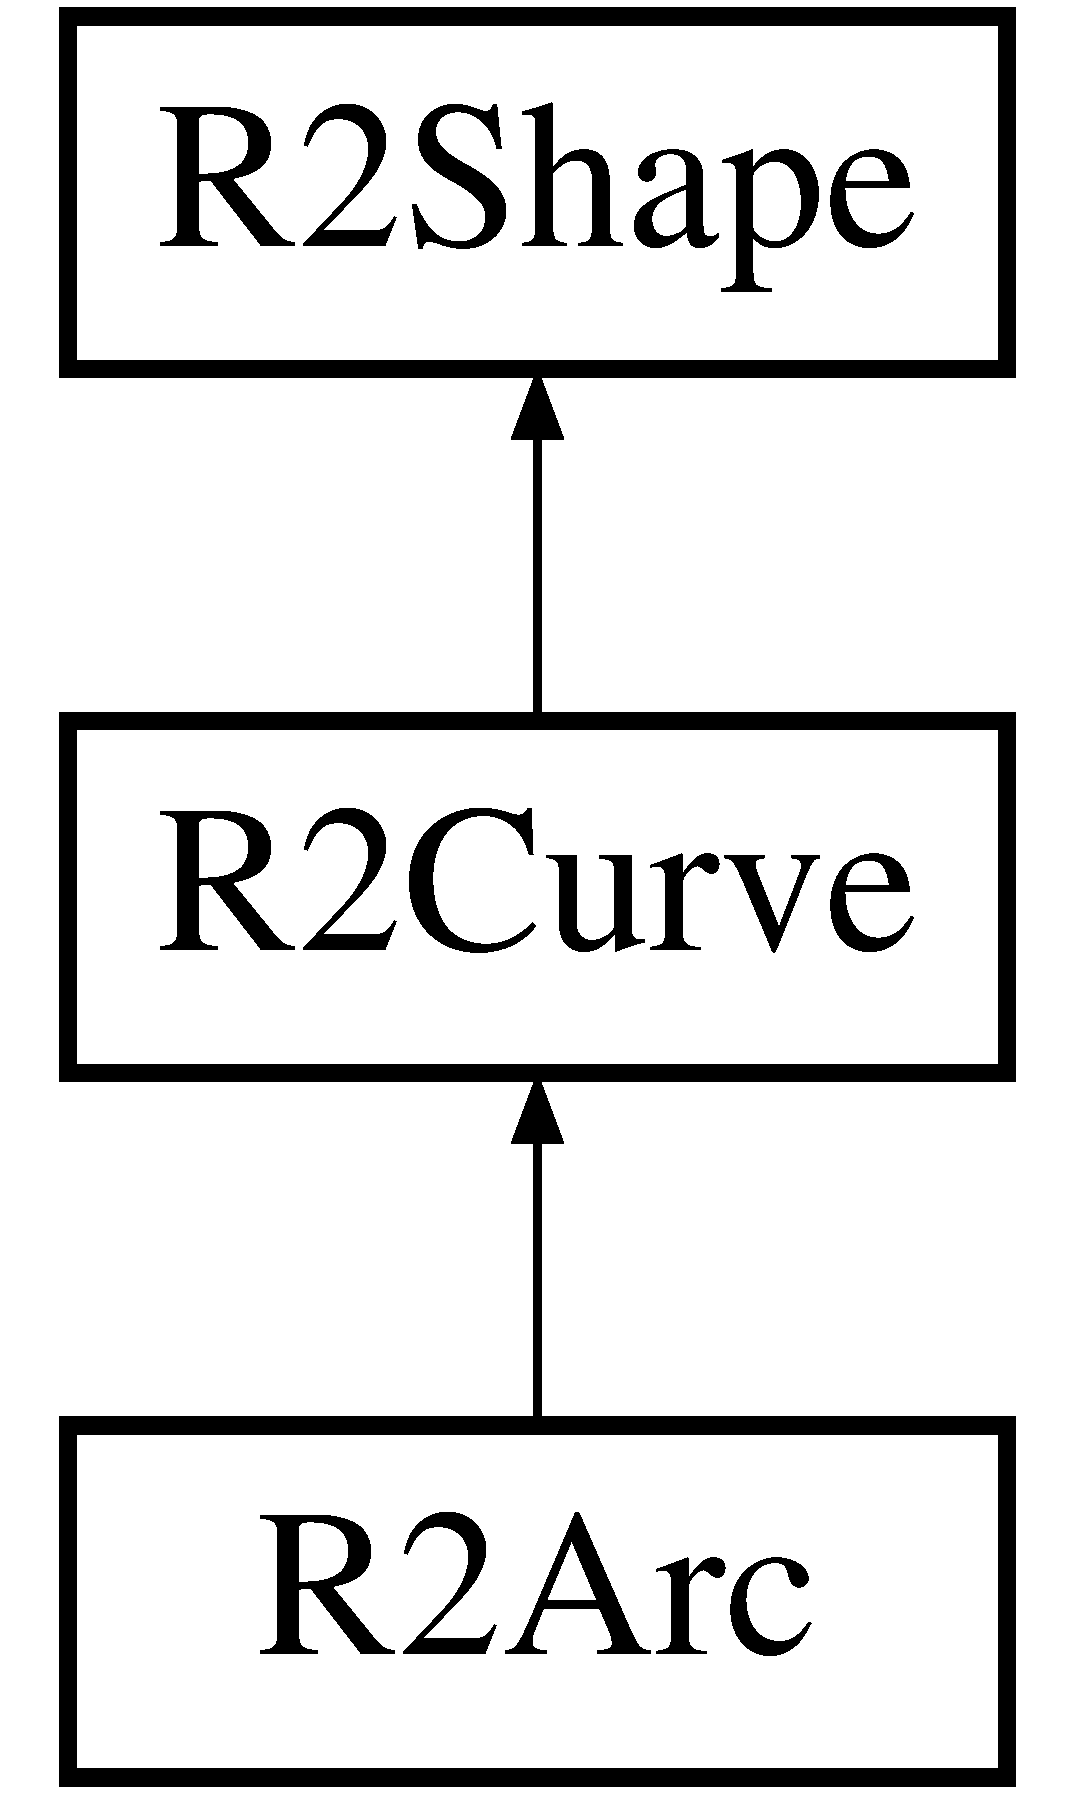
\includegraphics[height=3.000000cm]{class_r2_curve}
\end{center}
\end{figure}
\subsection*{Public Member Functions}
\begin{DoxyCompactItemize}
\item 
const R\+N\+Boolean {\bfseries Is\+Curve} (void) const \hypertarget{class_r2_curve_a161ea347c738099e4d2ae8a92129cec7}{}\label{class_r2_curve_a161ea347c738099e4d2ae8a92129cec7}

\end{DoxyCompactItemize}


The documentation for this class was generated from the following files\+:\begin{DoxyCompactItemize}
\item 
R2\+Shapes/R2\+Curve.\+h\item 
R2\+Shapes/R2\+Curve.\+cpp\end{DoxyCompactItemize}

\hypertarget{class_r2_diad}{}\section{R2\+Diad Class Reference}
\label{class_r2_diad}\index{R2\+Diad@{R2\+Diad}}
\subsection*{Public Member Functions}
\begin{DoxyCompactItemize}
\item 
{\bfseries R2\+Diad} (const \hyperlink{class_r2_diad}{R2\+Diad} \&diad)\hypertarget{class_r2_diad_abb68c6884b7c3a682cbf83c26b4d7066}{}\label{class_r2_diad_abb68c6884b7c3a682cbf83c26b4d7066}

\item 
{\bfseries R2\+Diad} (const \hyperlink{class_r2_vector}{R2\+Vector} \&xaxis, const \hyperlink{class_r2_vector}{R2\+Vector} \&yaxis)\hypertarget{class_r2_diad_ae6d1d1daf2b9cdae29aaf3b750715d48}{}\label{class_r2_diad_ae6d1d1daf2b9cdae29aaf3b750715d48}

\item 
const \hyperlink{class_r3_matrix}{R3\+Matrix} {\bfseries Matrix} (void) const \hypertarget{class_r2_diad_a2d8f6d127bc8a123171680a5eafcd61c}{}\label{class_r2_diad_a2d8f6d127bc8a123171680a5eafcd61c}

\item 
const \hyperlink{class_r3_matrix}{R3\+Matrix} {\bfseries Inverse\+Matrix} (void) const \hypertarget{class_r2_diad_a6673cdcb760c501ff9735b35e55d7fa0}{}\label{class_r2_diad_a6673cdcb760c501ff9735b35e55d7fa0}

\item 
const \hyperlink{class_r2_vector}{R2\+Vector} \& {\bfseries Axis} (R\+N\+Dimension dim) const \hypertarget{class_r2_diad_aab24b633fd70dcb173bd7de1f35cf198}{}\label{class_r2_diad_aab24b633fd70dcb173bd7de1f35cf198}

\item 
const \hyperlink{class_r2_vector}{R2\+Vector} \& {\bfseries operator\mbox{[}$\,$\mbox{]}} (R\+N\+Dimension dim) const \hypertarget{class_r2_diad_a9ea4e168f2de5716ac151ed042488952}{}\label{class_r2_diad_a9ea4e168f2de5716ac151ed042488952}

\item 
const R\+N\+Boolean {\bfseries operator==} (const \hyperlink{class_r2_diad}{R2\+Diad} \&diad) const \hypertarget{class_r2_diad_a2ee8bc22300b8014c2450dc4fa81d795}{}\label{class_r2_diad_a2ee8bc22300b8014c2450dc4fa81d795}

\item 
const R\+N\+Boolean {\bfseries operator!=} (const \hyperlink{class_r2_diad}{R2\+Diad} \&diad) const \hypertarget{class_r2_diad_a3820465b0424d7d66946667a7efdcd4d}{}\label{class_r2_diad_a3820465b0424d7d66946667a7efdcd4d}

\item 
void {\bfseries Normalize} (void)\hypertarget{class_r2_diad_a31fbd5298c4f786987f30cdf19b6f0ac}{}\label{class_r2_diad_a31fbd5298c4f786987f30cdf19b6f0ac}

\item 
void {\bfseries Rotate} (R\+N\+Angle radians)\hypertarget{class_r2_diad_a92ff1c2b210ae3288458be8509f3f0a9}{}\label{class_r2_diad_a92ff1c2b210ae3288458be8509f3f0a9}

\item 
void {\bfseries Mirror} (const \hyperlink{class_r2_line}{R2\+Line} \&line)\hypertarget{class_r2_diad_a9046b59c31f647bbc7a4f0015e0baee4}{}\label{class_r2_diad_a9046b59c31f647bbc7a4f0015e0baee4}

\item 
void {\bfseries Transform} (const \hyperlink{class_r2_transformation}{R2\+Transformation} \&transformation)\hypertarget{class_r2_diad_acbf21f28c4e64f7ddcc16f0dae9b36f7}{}\label{class_r2_diad_acbf21f28c4e64f7ddcc16f0dae9b36f7}

\item 
void {\bfseries Inverse\+Transform} (const \hyperlink{class_r2_transformation}{R2\+Transformation} \&transformation)\hypertarget{class_r2_diad_a080ff5f58e3dd9de0ad014fb07821729}{}\label{class_r2_diad_a080ff5f58e3dd9de0ad014fb07821729}

\item 
\hyperlink{class_r2_diad}{R2\+Diad} \& {\bfseries operator=} (const \hyperlink{class_r2_diad}{R2\+Diad} \&diad)\hypertarget{class_r2_diad_adc02ba0856a84870446a3507eae924e6}{}\label{class_r2_diad_adc02ba0856a84870446a3507eae924e6}

\item 
void {\bfseries Draw} (void) const \hypertarget{class_r2_diad_ac1fc795506cfd603c2d91d15fc28f251}{}\label{class_r2_diad_ac1fc795506cfd603c2d91d15fc28f251}

\item 
void {\bfseries Outline} (void) const \hypertarget{class_r2_diad_a71677d938a51cb6f27757d91f6412e75}{}\label{class_r2_diad_a71677d938a51cb6f27757d91f6412e75}

\end{DoxyCompactItemize}


The documentation for this class was generated from the following files\+:\begin{DoxyCompactItemize}
\item 
R2\+Shapes/R2\+Diad.\+h\item 
R2\+Shapes/R2\+Diad.\+cpp\end{DoxyCompactItemize}

\hypertarget{class_r2_grid}{}\section{R2\+Grid Class Reference}
\label{class_r2_grid}\index{R2\+Grid@{R2\+Grid}}
\subsection*{Public Member Functions}
\begin{DoxyCompactItemize}
\item 
{\bfseries R2\+Grid} (int xresolution=0, int yresolution=0)\hypertarget{class_r2_grid_a85fb6c5bbe1604799d6a23570898a5d4}{}\label{class_r2_grid_a85fb6c5bbe1604799d6a23570898a5d4}

\item 
{\bfseries R2\+Grid} (int xresolution, int yresolution, const \hyperlink{class_r2_box}{R2\+Box} \&bbox)\hypertarget{class_r2_grid_ab1e4369e4b74b47008561b020ac50187}{}\label{class_r2_grid_ab1e4369e4b74b47008561b020ac50187}

\item 
{\bfseries R2\+Grid} (int xresolution, int yresolution, const \hyperlink{class_r2_affine}{R2\+Affine} \&world\+\_\+to\+\_\+grid)\hypertarget{class_r2_grid_a7debe5ee1a944d7787bacfd52eb0c315}{}\label{class_r2_grid_a7debe5ee1a944d7787bacfd52eb0c315}

\item 
{\bfseries R2\+Grid} (const \hyperlink{class_r2_grid}{R2\+Grid} \&grid, int x1, int y1, int x2, int y2)\hypertarget{class_r2_grid_aefd751d856695545534c1629a3593466}{}\label{class_r2_grid_aefd751d856695545534c1629a3593466}

\item 
{\bfseries R2\+Grid} (const \hyperlink{class_r2_grid}{R2\+Grid} \&grid)\hypertarget{class_r2_grid_afde2d4292d0dc538b5d5a3e019628caf}{}\label{class_r2_grid_afde2d4292d0dc538b5d5a3e019628caf}

\item 
{\bfseries R2\+Grid} (const \hyperlink{class_r2_image}{R2\+Image} \&image, int dummy)\hypertarget{class_r2_grid_a2af06c7359701028e9ce052797dce42a}{}\label{class_r2_grid_a2af06c7359701028e9ce052797dce42a}

\item 
int {\bfseries N\+Entries} () const \hypertarget{class_r2_grid_aef1211e455ff1a66fa2793e214b3a006}{}\label{class_r2_grid_aef1211e455ff1a66fa2793e214b3a006}

\item 
int {\bfseries X\+Resolution} (void) const \hypertarget{class_r2_grid_a38d8f734206ce7b29357c6e155a7e75b}{}\label{class_r2_grid_a38d8f734206ce7b29357c6e155a7e75b}

\item 
int {\bfseries Y\+Resolution} (void) const \hypertarget{class_r2_grid_a418d4643f2fe864977bbf1100ab8b222}{}\label{class_r2_grid_a418d4643f2fe864977bbf1100ab8b222}

\item 
int {\bfseries Resolution} (R\+N\+Dimension dim) const \hypertarget{class_r2_grid_a321ef5029f5943b50dc4d277bf52e048}{}\label{class_r2_grid_a321ef5029f5943b50dc4d277bf52e048}

\item 
R\+N\+Scalar {\bfseries Sum} (void) const \hypertarget{class_r2_grid_a064f527488e010c0417d06c0ea92bcc8}{}\label{class_r2_grid_a064f527488e010c0417d06c0ea92bcc8}

\item 
R\+N\+Scalar {\bfseries Mean} (void) const \hypertarget{class_r2_grid_a45676187266aa1ec496ae89e13023482}{}\label{class_r2_grid_a45676187266aa1ec496ae89e13023482}

\item 
R\+N\+Scalar {\bfseries Median} (void) const \hypertarget{class_r2_grid_ad7df5122bc174b5ae7ff6d369d6e3bf6}{}\label{class_r2_grid_ad7df5122bc174b5ae7ff6d369d6e3bf6}

\item 
R\+N\+Scalar {\bfseries Maximum} (void) const \hypertarget{class_r2_grid_aba84db6b270da0785849a66a12a9cd33}{}\label{class_r2_grid_aba84db6b270da0785849a66a12a9cd33}

\item 
R\+N\+Scalar {\bfseries Minimum} (void) const \hypertarget{class_r2_grid_a81c9da7c7e0cedb10f8631af224db03e}{}\label{class_r2_grid_a81c9da7c7e0cedb10f8631af224db03e}

\item 
\hyperlink{class_r_n_interval}{R\+N\+Interval} {\bfseries Range} (void) const \hypertarget{class_r2_grid_a3e22ebb96b5dbe51861f5251b9682235}{}\label{class_r2_grid_a3e22ebb96b5dbe51861f5251b9682235}

\item 
R\+N\+Scalar {\bfseries L1\+Norm} (void) const \hypertarget{class_r2_grid_a192085b37efc61ebce36904bb2a87f51}{}\label{class_r2_grid_a192085b37efc61ebce36904bb2a87f51}

\item 
R\+N\+Scalar {\bfseries L2\+Norm} (void) const \hypertarget{class_r2_grid_a19604d4cc59545c44b457947f10ab0fd}{}\label{class_r2_grid_a19604d4cc59545c44b457947f10ab0fd}

\item 
R\+N\+Scalar {\bfseries Area} (void) const \hypertarget{class_r2_grid_a2ac1dbaee0106cce7b63f3004d25f502}{}\label{class_r2_grid_a2ac1dbaee0106cce7b63f3004d25f502}

\item 
int {\bfseries Cardinality} (void) const \hypertarget{class_r2_grid_aac8ae614d9148e2f3ecfa3c577cc3022}{}\label{class_r2_grid_aac8ae614d9148e2f3ecfa3c577cc3022}

\item 
\hyperlink{class_r2_box}{R2\+Box} {\bfseries Grid\+Box} (void) const \hypertarget{class_r2_grid_a861292fc29d4e2fee0572d4eb345cb0a}{}\label{class_r2_grid_a861292fc29d4e2fee0572d4eb345cb0a}

\item 
\hyperlink{class_r2_box}{R2\+Box} {\bfseries World\+Box} (void) const \hypertarget{class_r2_grid_ac9728ec945398ce1e5790d71a30c4dd0}{}\label{class_r2_grid_ac9728ec945398ce1e5790d71a30c4dd0}

\item 
const \hyperlink{class_r2_affine}{R2\+Affine} \& {\bfseries World\+To\+Grid\+Transformation} (void) const \hypertarget{class_r2_grid_a838c13ecb2cb107d6a5d28a26071da4c}{}\label{class_r2_grid_a838c13ecb2cb107d6a5d28a26071da4c}

\item 
const \hyperlink{class_r2_affine}{R2\+Affine} \& {\bfseries Grid\+To\+World\+Transformation} (void) const \hypertarget{class_r2_grid_a0b8d8fcfa7c28cc83a22f442e40def08}{}\label{class_r2_grid_a0b8d8fcfa7c28cc83a22f442e40def08}

\item 
R\+N\+Scalar {\bfseries World\+To\+Grid\+Scale\+Factor} (void) const \hypertarget{class_r2_grid_aa3c4cf4eb6ec3b53e6565d56a547389e}{}\label{class_r2_grid_aa3c4cf4eb6ec3b53e6565d56a547389e}

\item 
R\+N\+Scalar {\bfseries Grid\+To\+World\+Scale\+Factor} (void) const \hypertarget{class_r2_grid_ac1fa8422826106729cfe6471fa169995}{}\label{class_r2_grid_ac1fa8422826106729cfe6471fa169995}

\item 
R\+N\+Scalar {\bfseries Grid\+Value} (int index) const \hypertarget{class_r2_grid_a3d4fb1adf7c6ad8008eacd60c6fb444b}{}\label{class_r2_grid_a3d4fb1adf7c6ad8008eacd60c6fb444b}

\item 
R\+N\+Scalar {\bfseries Grid\+Value} (int i, int j) const \hypertarget{class_r2_grid_a0d22350f9a6e483a898d60b4514231d3}{}\label{class_r2_grid_a0d22350f9a6e483a898d60b4514231d3}

\item 
R\+N\+Scalar {\bfseries Grid\+Value} (R\+N\+Coord x, R\+N\+Coord y) const \hypertarget{class_r2_grid_a848cdfc1015bd14499914683d185daf0}{}\label{class_r2_grid_a848cdfc1015bd14499914683d185daf0}

\item 
R\+N\+Scalar {\bfseries Grid\+Value} (const \hyperlink{class_r2_point}{R2\+Point} \&grid\+\_\+point) const \hypertarget{class_r2_grid_a6f1ccc66b440d81904b2ebab6f01a02c}{}\label{class_r2_grid_a6f1ccc66b440d81904b2ebab6f01a02c}

\item 
R\+N\+Scalar {\bfseries World\+Value} (R\+N\+Coord x, R\+N\+Coord y) const \hypertarget{class_r2_grid_a340a7b0f3b79dff2cbc136d231680dea}{}\label{class_r2_grid_a340a7b0f3b79dff2cbc136d231680dea}

\item 
R\+N\+Scalar {\bfseries World\+Value} (const \hyperlink{class_r2_point}{R2\+Point} \&world\+\_\+point) const \hypertarget{class_r2_grid_a92ad86cf4389c62a4ef20209982a6d98}{}\label{class_r2_grid_a92ad86cf4389c62a4ef20209982a6d98}

\item 
R\+N\+Scalar \& {\bfseries operator()} (int i, int j)\hypertarget{class_r2_grid_a453059226abc07dcb83da0b24c415e67}{}\label{class_r2_grid_a453059226abc07dcb83da0b24c415e67}

\item 
R\+N\+Scalar \& {\bfseries operator()} (int i)\hypertarget{class_r2_grid_a891a72a9f832c109ef478e36e75aa345}{}\label{class_r2_grid_a891a72a9f832c109ef478e36e75aa345}

\item 
void {\bfseries Abs} (void)\hypertarget{class_r2_grid_acf4d6434c17703178785c1c893b3b58b}{}\label{class_r2_grid_acf4d6434c17703178785c1c893b3b58b}

\item 
void {\bfseries Sqrt} (void)\hypertarget{class_r2_grid_a5dac580b5d6014f1a3f829ab99f9c9a2}{}\label{class_r2_grid_a5dac580b5d6014f1a3f829ab99f9c9a2}

\item 
void {\bfseries Square} (void)\hypertarget{class_r2_grid_af00c2203810898918c15037631953d5a}{}\label{class_r2_grid_af00c2203810898918c15037631953d5a}

\item 
void {\bfseries Negate} (void)\hypertarget{class_r2_grid_aa1c4326dcd902007c128f8efb02e9109}{}\label{class_r2_grid_aa1c4326dcd902007c128f8efb02e9109}

\item 
void {\bfseries Invert} (void)\hypertarget{class_r2_grid_abd465e0802735efc064e049da7ffe25d}{}\label{class_r2_grid_abd465e0802735efc064e049da7ffe25d}

\item 
void {\bfseries Transpose} (void)\hypertarget{class_r2_grid_a93a84bdfbf008e038b7d2a14f9c83923}{}\label{class_r2_grid_a93a84bdfbf008e038b7d2a14f9c83923}

\item 
void {\bfseries Normalize} (void)\hypertarget{class_r2_grid_ac39576558a8509cbd96cb373feab50f1}{}\label{class_r2_grid_ac39576558a8509cbd96cb373feab50f1}

\item 
void {\bfseries Laplacian} (void)\hypertarget{class_r2_grid_a4a810951ece1915e860751de691a93b1}{}\label{class_r2_grid_a4a810951ece1915e860751de691a93b1}

\item 
void {\bfseries Laplacian} (R\+N\+Dimension dim)\hypertarget{class_r2_grid_ac747e8a1da252ca6bbbe22bf8deac6ff}{}\label{class_r2_grid_ac747e8a1da252ca6bbbe22bf8deac6ff}

\item 
void {\bfseries Sobel} (void)\hypertarget{class_r2_grid_acc6dbe6f7b6c8685c7c1d1ae04cfff18}{}\label{class_r2_grid_acc6dbe6f7b6c8685c7c1d1ae04cfff18}

\item 
void {\bfseries Gradient\+Angle} (void)\hypertarget{class_r2_grid_a870983d53f0430255323072b4e9e3e68}{}\label{class_r2_grid_a870983d53f0430255323072b4e9e3e68}

\item 
void {\bfseries Gradient\+Magnitude} (void)\hypertarget{class_r2_grid_a08f6db8a58ee1a82542d4f35c057cfab}{}\label{class_r2_grid_a08f6db8a58ee1a82542d4f35c057cfab}

\item 
void {\bfseries Gradient} (R\+N\+Dimension dim)\hypertarget{class_r2_grid_a06afa5bd3409c01a5cd93c644ba206ad}{}\label{class_r2_grid_a06afa5bd3409c01a5cd93c644ba206ad}

\item 
void {\bfseries Hessian} (R\+N\+Dimension dim1, R\+N\+Dimension dim2)\hypertarget{class_r2_grid_ad889ddffd80f4fa1fb0f6e02c20b4fe2}{}\label{class_r2_grid_ad889ddffd80f4fa1fb0f6e02c20b4fe2}

\item 
void {\bfseries Clear} (R\+N\+Scalar value=0)\hypertarget{class_r2_grid_a2e5fd6336f4d4002cfd73bb443a77cb1}{}\label{class_r2_grid_a2e5fd6336f4d4002cfd73bb443a77cb1}

\item 
void {\bfseries Detect\+Edges} (void)\hypertarget{class_r2_grid_a3f00116a23b6a3d8faa0379bf9f4d3e0}{}\label{class_r2_grid_a3f00116a23b6a3d8faa0379bf9f4d3e0}

\item 
void {\bfseries Detect\+Corners} (void)\hypertarget{class_r2_grid_a5de2ac96fa22596e9199099418212d08}{}\label{class_r2_grid_a5de2ac96fa22596e9199099418212d08}

\item 
void {\bfseries Fill\+Holes} (void)\hypertarget{class_r2_grid_ae3dd6e55fed559fcb84ce636b95a1a48}{}\label{class_r2_grid_ae3dd6e55fed559fcb84ce636b95a1a48}

\item 
void {\bfseries Fill\+Holes} (int max\+\_\+hole\+\_\+size)\hypertarget{class_r2_grid_a84453eecbcf8e8be8e7539da4fb0d797}{}\label{class_r2_grid_a84453eecbcf8e8be8e7539da4fb0d797}

\item 
void {\bfseries Dilate} (R\+N\+Scalar grid\+\_\+distance)\hypertarget{class_r2_grid_a5a6064c32ba76f6850f54a3a6aea4f36}{}\label{class_r2_grid_a5a6064c32ba76f6850f54a3a6aea4f36}

\item 
void {\bfseries Erode} (R\+N\+Scalar grid\+\_\+distance)\hypertarget{class_r2_grid_a0909da02a698c392f12a4407524566fb}{}\label{class_r2_grid_a0909da02a698c392f12a4407524566fb}

\item 
void {\bfseries Blur} (R\+N\+Scalar grid\+\_\+sigma=2)\hypertarget{class_r2_grid_a9ad95b5f2e2cf90faa944869e3345b26}{}\label{class_r2_grid_a9ad95b5f2e2cf90faa944869e3345b26}

\item 
void {\bfseries Blur} (R\+N\+Dimension dim, R\+N\+Scalar grid\+\_\+sigma)\hypertarget{class_r2_grid_af32163f0fcf74a7dca9fc6df3770d99a}{}\label{class_r2_grid_af32163f0fcf74a7dca9fc6df3770d99a}

\item 
void {\bfseries Harris\+Corner\+Filter} (int grid\+\_\+radius=3, R\+N\+Scalar kappa=0.\+05)\hypertarget{class_r2_grid_adf04ce6ecff9875c546f2a46a7bc7319}{}\label{class_r2_grid_adf04ce6ecff9875c546f2a46a7bc7319}

\item 
void {\bfseries Bilateral\+Filter} (R\+N\+Length grid\+\_\+sigma=2, R\+N\+Scalar value\+\_\+sigma=-\/1)\hypertarget{class_r2_grid_a83e989d8e62a7d7ee43dbeafbfbdbdd6}{}\label{class_r2_grid_a83e989d8e62a7d7ee43dbeafbfbdbdd6}

\item 
void {\bfseries Anisotropic\+Diffusion} (R\+N\+Length grid\+\_\+sigma=2, R\+N\+Scalar gradient\+\_\+sigma=-\/1)\hypertarget{class_r2_grid_a4194e9d7286046de85d260f305fc6653}{}\label{class_r2_grid_a4194e9d7286046de85d260f305fc6653}

\item 
void {\bfseries Percentile\+Filter} (R\+N\+Length grid\+\_\+radius, R\+N\+Scalar percentile)\hypertarget{class_r2_grid_aa940a310e7bd638ae9c118079e375902}{}\label{class_r2_grid_aa940a310e7bd638ae9c118079e375902}

\item 
void {\bfseries Min\+Filter} (R\+N\+Length grid\+\_\+radius)\hypertarget{class_r2_grid_a11742d7b9fd758b08bfd0acf7bdb62ac}{}\label{class_r2_grid_a11742d7b9fd758b08bfd0acf7bdb62ac}

\item 
void {\bfseries Max\+Filter} (R\+N\+Length grid\+\_\+radius)\hypertarget{class_r2_grid_a8a0709f1eaa5f31c02ac38ba9dc987da}{}\label{class_r2_grid_a8a0709f1eaa5f31c02ac38ba9dc987da}

\item 
void {\bfseries Median\+Filter} (R\+N\+Length grid\+\_\+radius)\hypertarget{class_r2_grid_a369b22051996257242565130aaa64396}{}\label{class_r2_grid_a369b22051996257242565130aaa64396}

\item 
void {\bfseries Mask\+Non\+Minima} (R\+N\+Length grid\+\_\+radius=0)\hypertarget{class_r2_grid_aa1e748910b9deced3d1163a0160cb982}{}\label{class_r2_grid_aa1e748910b9deced3d1163a0160cb982}

\item 
void {\bfseries Mask\+Non\+Maxima} (R\+N\+Length grid\+\_\+radius=0)\hypertarget{class_r2_grid_ad0050370c1be4284a3547504bf280683}{}\label{class_r2_grid_ad0050370c1be4284a3547504bf280683}

\item 
void {\bfseries Convolve} (const R\+N\+Scalar filter\mbox{[}3\mbox{]}\mbox{[}3\mbox{]})\hypertarget{class_r2_grid_a3eaad035ffd71c3383e4a8cbaeb1a422}{}\label{class_r2_grid_a3eaad035ffd71c3383e4a8cbaeb1a422}

\item 
void {\bfseries Substitute} (R\+N\+Scalar old\+\_\+value, R\+N\+Scalar new\+\_\+value)\hypertarget{class_r2_grid_a5479d2aceb4cea6cb4611b6256cb7987}{}\label{class_r2_grid_a5479d2aceb4cea6cb4611b6256cb7987}

\item 
void {\bfseries Add} (R\+N\+Scalar value)\hypertarget{class_r2_grid_a4062b8d0c337df580b5ebb304d4975ad}{}\label{class_r2_grid_a4062b8d0c337df580b5ebb304d4975ad}

\item 
void {\bfseries Add} (const \hyperlink{class_r2_grid}{R2\+Grid} \&grid)\hypertarget{class_r2_grid_ad869fb99bea38f7bb71ff2f39ae695c9}{}\label{class_r2_grid_ad869fb99bea38f7bb71ff2f39ae695c9}

\item 
void {\bfseries Subtract} (R\+N\+Scalar value)\hypertarget{class_r2_grid_a2581a386310783375a8f3f8fe2949782}{}\label{class_r2_grid_a2581a386310783375a8f3f8fe2949782}

\item 
void {\bfseries Subtract} (const \hyperlink{class_r2_grid}{R2\+Grid} \&grid)\hypertarget{class_r2_grid_a94b3e3cf043c0fd35cb2bdc1b57bb49c}{}\label{class_r2_grid_a94b3e3cf043c0fd35cb2bdc1b57bb49c}

\item 
void {\bfseries Multiply} (R\+N\+Scalar value)\hypertarget{class_r2_grid_aec87288efd69a0f64df28eace979ead8}{}\label{class_r2_grid_aec87288efd69a0f64df28eace979ead8}

\item 
void {\bfseries Multiply} (const \hyperlink{class_r2_grid}{R2\+Grid} \&grid)\hypertarget{class_r2_grid_ace0b28e792c256e85c14863f23af10ef}{}\label{class_r2_grid_ace0b28e792c256e85c14863f23af10ef}

\item 
void {\bfseries Divide} (R\+N\+Scalar value)\hypertarget{class_r2_grid_a499fac85cb2532e6f211865479cee705}{}\label{class_r2_grid_a499fac85cb2532e6f211865479cee705}

\item 
void {\bfseries Divide} (const \hyperlink{class_r2_grid}{R2\+Grid} \&grid)\hypertarget{class_r2_grid_af459fcae09895573406007f47b6f2e65}{}\label{class_r2_grid_af459fcae09895573406007f47b6f2e65}

\item 
void {\bfseries Pow} (R\+N\+Scalar exponent)\hypertarget{class_r2_grid_aa189d7e0e45f4fb21ac81fe3359c3c62}{}\label{class_r2_grid_aa189d7e0e45f4fb21ac81fe3359c3c62}

\item 
void {\bfseries Mask} (const \hyperlink{class_r2_grid}{R2\+Grid} \&grid)\hypertarget{class_r2_grid_aca78f02c6be6057682305a4825fd1c80}{}\label{class_r2_grid_aca78f02c6be6057682305a4825fd1c80}

\item 
void {\bfseries Overlay} (const \hyperlink{class_r2_grid}{R2\+Grid} \&grid)\hypertarget{class_r2_grid_ae439f68642fc138f4398a58d327d7ed9}{}\label{class_r2_grid_ae439f68642fc138f4398a58d327d7ed9}

\item 
void {\bfseries Threshold} (R\+N\+Scalar threshold, R\+N\+Scalar low, R\+N\+Scalar high)\hypertarget{class_r2_grid_a528045cd7443221554a885a812704cde}{}\label{class_r2_grid_a528045cd7443221554a885a812704cde}

\item 
void {\bfseries Threshold} (const \hyperlink{class_r2_grid}{R2\+Grid} \&threshold, R\+N\+Scalar low, R\+N\+Scalar high)\hypertarget{class_r2_grid_a271ede56d0335b775012a9896996790f}{}\label{class_r2_grid_a271ede56d0335b775012a9896996790f}

\item 
void {\bfseries Signed\+Distance\+Transform} (void)\hypertarget{class_r2_grid_aa9b39f779a4d182a77cf32bb2b025b72}{}\label{class_r2_grid_aa9b39f779a4d182a77cf32bb2b025b72}

\item 
void {\bfseries Squared\+Distance\+Transform} (void)\hypertarget{class_r2_grid_a79b7990342f02e6ad2f068dbcf68306a}{}\label{class_r2_grid_a79b7990342f02e6ad2f068dbcf68306a}

\item 
void {\bfseries Voronoi} (\hyperlink{class_r2_grid}{R2\+Grid} $\ast$squared\+\_\+distance\+\_\+grid=N\+U\+LL)\hypertarget{class_r2_grid_ae79769dadc262f29bcdbe3d9330b0d65}{}\label{class_r2_grid_ae79769dadc262f29bcdbe3d9330b0d65}

\item 
void {\bfseries Point\+Symmetry\+Transform} (int radius=-\/1)\hypertarget{class_r2_grid_a361d567562753139f92d1ae5603d1983}{}\label{class_r2_grid_a361d567562753139f92d1ae5603d1983}

\item 
void {\bfseries Gauss} (R\+N\+Length sigma=sqrt(8.\+0), R\+N\+Boolean square=T\+R\+UE)\hypertarget{class_r2_grid_a434b7fb302a2964e02e7ed1f40375eac}{}\label{class_r2_grid_a434b7fb302a2964e02e7ed1f40375eac}

\item 
void {\bfseries Resample} (int xres, int yres)\hypertarget{class_r2_grid_af69f341ffdbf7dae6bf6aab40418339f}{}\label{class_r2_grid_af69f341ffdbf7dae6bf6aab40418339f}

\item 
void {\bfseries Pad\+With\+Zero} (int xres, int yres)\hypertarget{class_r2_grid_ae737c0d12e04d2a968b130722d930f24}{}\label{class_r2_grid_ae737c0d12e04d2a968b130722d930f24}

\item 
void {\bfseries Set\+Grid\+Value} (int index, R\+N\+Scalar value)\hypertarget{class_r2_grid_a40acc54412cf755e2a4127653c7ae387}{}\label{class_r2_grid_a40acc54412cf755e2a4127653c7ae387}

\item 
void {\bfseries Set\+Grid\+Value} (int i, int j, R\+N\+Scalar value)\hypertarget{class_r2_grid_a58ad32806649ee4368566fa8dfdca6e8}{}\label{class_r2_grid_a58ad32806649ee4368566fa8dfdca6e8}

\item 
void {\bfseries Add\+Grid\+Value} (int i, int j, R\+N\+Scalar value)\hypertarget{class_r2_grid_afe890811aa3948be377cef90d448020b}{}\label{class_r2_grid_afe890811aa3948be377cef90d448020b}

\item 
\hyperlink{class_r2_grid}{R2\+Grid} \& {\bfseries operator=} (const \hyperlink{class_r2_grid}{R2\+Grid} \&grid)\hypertarget{class_r2_grid_a4a313d794d0e30ff4825549da52231b1}{}\label{class_r2_grid_a4a313d794d0e30ff4825549da52231b1}

\item 
\hyperlink{class_r2_grid}{R2\+Grid} \& {\bfseries operator+=} (R\+N\+Scalar scale)\hypertarget{class_r2_grid_a0f8fe4b16c4411ab683b3117d3f4efc7}{}\label{class_r2_grid_a0f8fe4b16c4411ab683b3117d3f4efc7}

\item 
\hyperlink{class_r2_grid}{R2\+Grid} \& {\bfseries operator+=} (const \hyperlink{class_r2_grid}{R2\+Grid} \&grid)\hypertarget{class_r2_grid_a020cce55debadafe5e86e51ab252d071}{}\label{class_r2_grid_a020cce55debadafe5e86e51ab252d071}

\item 
\hyperlink{class_r2_grid}{R2\+Grid} \& {\bfseries operator-\/=} (R\+N\+Scalar scale)\hypertarget{class_r2_grid_a0df9628c0d746cd1754539991d865bb2}{}\label{class_r2_grid_a0df9628c0d746cd1754539991d865bb2}

\item 
\hyperlink{class_r2_grid}{R2\+Grid} \& {\bfseries operator-\/=} (const \hyperlink{class_r2_grid}{R2\+Grid} \&grid)\hypertarget{class_r2_grid_a0242b484d6787235de27305121d2e99f}{}\label{class_r2_grid_a0242b484d6787235de27305121d2e99f}

\item 
\hyperlink{class_r2_grid}{R2\+Grid} \& {\bfseries operator$\ast$=} (R\+N\+Scalar scale)\hypertarget{class_r2_grid_a95d1cafd1688252a1aeb8f4cd6b67889}{}\label{class_r2_grid_a95d1cafd1688252a1aeb8f4cd6b67889}

\item 
\hyperlink{class_r2_grid}{R2\+Grid} \& {\bfseries operator$\ast$=} (const \hyperlink{class_r2_grid}{R2\+Grid} \&grid)\hypertarget{class_r2_grid_aa696955204d7a82955499e4b4876d456}{}\label{class_r2_grid_aa696955204d7a82955499e4b4876d456}

\item 
\hyperlink{class_r2_grid}{R2\+Grid} \& {\bfseries operator/=} (R\+N\+Scalar scale)\hypertarget{class_r2_grid_a50cc7b84c7e46c12172c151569e815dc}{}\label{class_r2_grid_a50cc7b84c7e46c12172c151569e815dc}

\item 
\hyperlink{class_r2_grid}{R2\+Grid} \& {\bfseries operator/=} (const \hyperlink{class_r2_grid}{R2\+Grid} \&grid)\hypertarget{class_r2_grid_ad2b98153f5037e5d772a8a77c273c084}{}\label{class_r2_grid_ad2b98153f5037e5d772a8a77c273c084}

\item 
void {\bfseries Rasterize\+Grid\+Point} (R\+N\+Coord x, R\+N\+Coord y, R\+N\+Scalar value)\hypertarget{class_r2_grid_adc49ffcdfef261b27bc3bfbb655a033f}{}\label{class_r2_grid_adc49ffcdfef261b27bc3bfbb655a033f}

\item 
void {\bfseries Rasterize\+World\+Point} (R\+N\+Coord x, R\+N\+Coord y, R\+N\+Scalar value)\hypertarget{class_r2_grid_a9ed686100f41ed03693f991896cdc966}{}\label{class_r2_grid_a9ed686100f41ed03693f991896cdc966}

\item 
void {\bfseries Rasterize\+Grid\+Point} (const \hyperlink{class_r2_point}{R2\+Point} \&point, R\+N\+Scalar value)\hypertarget{class_r2_grid_af8d1d0070f23bc8406dc4779ed76ee03}{}\label{class_r2_grid_af8d1d0070f23bc8406dc4779ed76ee03}

\item 
void {\bfseries Rasterize\+World\+Point} (const \hyperlink{class_r2_point}{R2\+Point} \&point, R\+N\+Scalar value)\hypertarget{class_r2_grid_aa29e3cf55e60836162b3c4ed2f06fea1}{}\label{class_r2_grid_aa29e3cf55e60836162b3c4ed2f06fea1}

\item 
void {\bfseries Rasterize\+Grid\+Span} (const \hyperlink{class_r2_point}{R2\+Point} \&p1, const \hyperlink{class_r2_point}{R2\+Point} \&p2, R\+N\+Scalar value)\hypertarget{class_r2_grid_a9367fdb40411ed5d720a9dc6f9e56a94}{}\label{class_r2_grid_a9367fdb40411ed5d720a9dc6f9e56a94}

\item 
void {\bfseries Rasterize\+World\+Span} (const \hyperlink{class_r2_point}{R2\+Point} \&p1, const \hyperlink{class_r2_point}{R2\+Point} \&p2, R\+N\+Scalar value)\hypertarget{class_r2_grid_a6c4aa0a2f2b613c23bee6a9bb897df50}{}\label{class_r2_grid_a6c4aa0a2f2b613c23bee6a9bb897df50}

\item 
void {\bfseries Rasterize\+Grid\+Span} (const int p1\mbox{[}3\mbox{]}, const int p2\mbox{[}3\mbox{]}, R\+N\+Scalar value1, R\+N\+Scalar value2)\hypertarget{class_r2_grid_a474840b2af0023b4c26d9e1647c1c831}{}\label{class_r2_grid_a474840b2af0023b4c26d9e1647c1c831}

\item 
void {\bfseries Rasterize\+Grid\+Span} (const \hyperlink{class_r2_point}{R2\+Point} \&p1, const \hyperlink{class_r2_point}{R2\+Point} \&p2, R\+N\+Scalar value1, R\+N\+Scalar value2)\hypertarget{class_r2_grid_af47c16f3fcb7b3c3320d3132a03524fe}{}\label{class_r2_grid_af47c16f3fcb7b3c3320d3132a03524fe}

\item 
void {\bfseries Rasterize\+World\+Span} (const \hyperlink{class_r2_point}{R2\+Point} \&p1, const \hyperlink{class_r2_point}{R2\+Point} \&p2, R\+N\+Scalar value1, R\+N\+Scalar value2)\hypertarget{class_r2_grid_adc47db68ef062fec90193255c1750aea}{}\label{class_r2_grid_adc47db68ef062fec90193255c1750aea}

\item 
void {\bfseries Rasterize\+Grid\+Box} (const int p1\mbox{[}3\mbox{]}, const int p2\mbox{[}3\mbox{]}, R\+N\+Scalar value)\hypertarget{class_r2_grid_aa29e879ad7754e2fcdfa06b2bd524e7c}{}\label{class_r2_grid_aa29e879ad7754e2fcdfa06b2bd524e7c}

\item 
void {\bfseries Rasterize\+Grid\+Box} (const \hyperlink{class_r2_point}{R2\+Point} \&p1, const \hyperlink{class_r2_point}{R2\+Point} \&p2, R\+N\+Scalar value)\hypertarget{class_r2_grid_afdd7ed207ed8fdfd509ea999e7f27256}{}\label{class_r2_grid_afdd7ed207ed8fdfd509ea999e7f27256}

\item 
void {\bfseries Rasterize\+World\+Box} (const \hyperlink{class_r2_point}{R2\+Point} \&p1, const \hyperlink{class_r2_point}{R2\+Point} \&p2, R\+N\+Scalar value)\hypertarget{class_r2_grid_a676d91d5caa1d328a84c8c30ef8579a4}{}\label{class_r2_grid_a676d91d5caa1d328a84c8c30ef8579a4}

\item 
void {\bfseries Rasterize\+Grid\+Triangle} (const \hyperlink{class_r2_point}{R2\+Point} \&p1, const \hyperlink{class_r2_point}{R2\+Point} \&p2, const \hyperlink{class_r2_point}{R2\+Point} \&p3, R\+N\+Scalar value)\hypertarget{class_r2_grid_ab5d67a74e85bcf616809227db3ba60e1}{}\label{class_r2_grid_ab5d67a74e85bcf616809227db3ba60e1}

\item 
void {\bfseries Rasterize\+World\+Triangle} (const \hyperlink{class_r2_point}{R2\+Point} \&p1, const \hyperlink{class_r2_point}{R2\+Point} \&p2, const \hyperlink{class_r2_point}{R2\+Point} \&p3, R\+N\+Scalar value)\hypertarget{class_r2_grid_adaaab1b432d7bf370f99269c0c82978c}{}\label{class_r2_grid_adaaab1b432d7bf370f99269c0c82978c}

\item 
void {\bfseries Rasterize\+Grid\+Triangle} (const int p1\mbox{[}3\mbox{]}, const int p2\mbox{[}3\mbox{]}, const int p3\mbox{[}3\mbox{]}, R\+N\+Scalar value1, R\+N\+Scalar value2, R\+N\+Scalar value3)\hypertarget{class_r2_grid_ad9249ac86af74c8459d47d6292ea641f}{}\label{class_r2_grid_ad9249ac86af74c8459d47d6292ea641f}

\item 
void {\bfseries Rasterize\+Grid\+Triangle} (const \hyperlink{class_r2_point}{R2\+Point} \&p1, const \hyperlink{class_r2_point}{R2\+Point} \&p2, const \hyperlink{class_r2_point}{R2\+Point} \&p3, R\+N\+Scalar value1, R\+N\+Scalar value2, R\+N\+Scalar value3)\hypertarget{class_r2_grid_aed8bf8f2826dec2b1cd46718c0dad386}{}\label{class_r2_grid_aed8bf8f2826dec2b1cd46718c0dad386}

\item 
void {\bfseries Rasterize\+World\+Triangle} (const \hyperlink{class_r2_point}{R2\+Point} \&p1, const \hyperlink{class_r2_point}{R2\+Point} \&p2, const \hyperlink{class_r2_point}{R2\+Point} \&p3, R\+N\+Scalar value1, R\+N\+Scalar value2, R\+N\+Scalar value3)\hypertarget{class_r2_grid_ac26feb4c1725d1f933b404b272870283}{}\label{class_r2_grid_ac26feb4c1725d1f933b404b272870283}

\item 
void {\bfseries Rasterize\+Grid\+Circle} (const \hyperlink{class_r2_point}{R2\+Point} \&center, R\+N\+Length radius, R\+N\+Scalar value)\hypertarget{class_r2_grid_aee09a4a0730892bfe812e01e00a19e6d}{}\label{class_r2_grid_aee09a4a0730892bfe812e01e00a19e6d}

\item 
void {\bfseries Rasterize\+World\+Circle} (const \hyperlink{class_r2_point}{R2\+Point} \&center, R\+N\+Length radius, R\+N\+Scalar value)\hypertarget{class_r2_grid_a1a11499746e25be1afe9204efcfeb3f7}{}\label{class_r2_grid_a1a11499746e25be1afe9204efcfeb3f7}

\item 
void {\bfseries Rasterize\+Grid\+Polygon} (const \hyperlink{class_r2_polygon}{R2\+Polygon} \&polygon, R\+N\+Scalar value)\hypertarget{class_r2_grid_ab57017b16e9b39a8213a878dc75b09b0}{}\label{class_r2_grid_ab57017b16e9b39a8213a878dc75b09b0}

\item 
void {\bfseries Rasterize\+World\+Polygon} (const \hyperlink{class_r2_polygon}{R2\+Polygon} \&polygon, R\+N\+Scalar value)\hypertarget{class_r2_grid_a382463ad003dba7537cc60d34455b9d0}{}\label{class_r2_grid_a382463ad003dba7537cc60d34455b9d0}

\item 
R\+N\+Scalar {\bfseries Dot} (const \hyperlink{class_r2_grid}{R2\+Grid} \&grid) const \hypertarget{class_r2_grid_ab591a6c563ce99cde5bc56f0860ab1b6}{}\label{class_r2_grid_ab591a6c563ce99cde5bc56f0860ab1b6}

\item 
R\+N\+Scalar {\bfseries L1\+Distance} (const \hyperlink{class_r2_grid}{R2\+Grid} \&grid) const \hypertarget{class_r2_grid_a4c5e1ad6c45d7060f84f631c6b423c08}{}\label{class_r2_grid_a4c5e1ad6c45d7060f84f631c6b423c08}

\item 
R\+N\+Scalar {\bfseries L2\+Distance} (const \hyperlink{class_r2_grid}{R2\+Grid} \&grid) const \hypertarget{class_r2_grid_a262d42b110a9309fb72c6767f577cc7b}{}\label{class_r2_grid_a262d42b110a9309fb72c6767f577cc7b}

\item 
R\+N\+Scalar {\bfseries L2\+Distance\+Squared} (const \hyperlink{class_r2_grid}{R2\+Grid} \&grid) const \hypertarget{class_r2_grid_aff7cf5a83223b64ecc20e4ee2db0ba36}{}\label{class_r2_grid_aff7cf5a83223b64ecc20e4ee2db0ba36}

\item 
void {\bfseries Set\+World\+To\+Grid\+Transformation} (const \hyperlink{class_r2_affine}{R2\+Affine} \&affine)\hypertarget{class_r2_grid_a63087fcd7d32ffd8e8100b83af1ea134}{}\label{class_r2_grid_a63087fcd7d32ffd8e8100b83af1ea134}

\item 
void {\bfseries Set\+World\+To\+Grid\+Transformation} (const \hyperlink{class_r2_box}{R2\+Box} \&world\+\_\+box)\hypertarget{class_r2_grid_a4807b1c3a374aad3f64b6fd0442e6988}{}\label{class_r2_grid_a4807b1c3a374aad3f64b6fd0442e6988}

\item 
void {\bfseries Set\+World\+To\+Grid\+Transformation} (const \hyperlink{class_r2_point}{R2\+Point} \&world\+\_\+origin, const \hyperlink{class_r2_vector}{R2\+Vector} \&world\+\_\+xaxis, R\+N\+Length world\+\_\+radius)\hypertarget{class_r2_grid_a29c78ad5581c88f5e36556bfe58e5c5c}{}\label{class_r2_grid_a29c78ad5581c88f5e36556bfe58e5c5c}

\item 
\hyperlink{class_r2_point}{R2\+Point} {\bfseries World\+Position} (const \hyperlink{class_r2_point}{R2\+Point} \&grid\+\_\+point) const \hypertarget{class_r2_grid_af2466da8df11d5a4639350c4c91303f7}{}\label{class_r2_grid_af2466da8df11d5a4639350c4c91303f7}

\item 
\hyperlink{class_r2_point}{R2\+Point} {\bfseries Grid\+Position} (const \hyperlink{class_r2_point}{R2\+Point} \&world\+\_\+point) const \hypertarget{class_r2_grid_abc374c2517b4902df1828ec5d1bc2606}{}\label{class_r2_grid_abc374c2517b4902df1828ec5d1bc2606}

\item 
\hyperlink{class_r2_point}{R2\+Point} {\bfseries World\+Position} (R\+N\+Coord x, R\+N\+Coord y) const \hypertarget{class_r2_grid_a464dd15d3c537f5b83bf567d5381807c}{}\label{class_r2_grid_a464dd15d3c537f5b83bf567d5381807c}

\item 
\hyperlink{class_r2_point}{R2\+Point} {\bfseries Grid\+Position} (R\+N\+Coord x, R\+N\+Coord y) const \hypertarget{class_r2_grid_ad305f9a4842f78f9efdd09e2265677cd}{}\label{class_r2_grid_ad305f9a4842f78f9efdd09e2265677cd}

\item 
int {\bfseries Read\+File} (const char $\ast$filename)\hypertarget{class_r2_grid_a0004c5367be01d6e557a8a7da5eceb49}{}\label{class_r2_grid_a0004c5367be01d6e557a8a7da5eceb49}

\item 
int {\bfseries Read\+P\+F\+M\+File} (const char $\ast$filename)\hypertarget{class_r2_grid_a9ecc7a1e16aa59abeea1c3caa3c16e72}{}\label{class_r2_grid_a9ecc7a1e16aa59abeea1c3caa3c16e72}

\item 
int {\bfseries Read\+R\+A\+W\+File} (const char $\ast$filename)\hypertarget{class_r2_grid_a48f7bf22b01f9f5a48f5f6542389eecf}{}\label{class_r2_grid_a48f7bf22b01f9f5a48f5f6542389eecf}

\item 
int {\bfseries Read\+Grid\+File} (const char $\ast$filename)\hypertarget{class_r2_grid_a76a84b8211711eca6bbe39a527455281}{}\label{class_r2_grid_a76a84b8211711eca6bbe39a527455281}

\item 
int {\bfseries Read\+P\+N\+G\+File} (const char $\ast$filename)\hypertarget{class_r2_grid_a9325c88135f3082c0b6163e43a39760a}{}\label{class_r2_grid_a9325c88135f3082c0b6163e43a39760a}

\item 
int {\bfseries Read\+Image} (const char $\ast$filename)\hypertarget{class_r2_grid_a8059d2a7838e3e076892fbde26be60b8}{}\label{class_r2_grid_a8059d2a7838e3e076892fbde26be60b8}

\item 
int {\bfseries Write\+File} (const char $\ast$filename) const \hypertarget{class_r2_grid_a48200205e8835a520f02a5fc0d0bdb35}{}\label{class_r2_grid_a48200205e8835a520f02a5fc0d0bdb35}

\item 
int {\bfseries Write\+P\+F\+M\+File} (const char $\ast$filename) const \hypertarget{class_r2_grid_a67ed84304fd605f93562988d5b91f8a3}{}\label{class_r2_grid_a67ed84304fd605f93562988d5b91f8a3}

\item 
int {\bfseries Write\+R\+A\+W\+File} (const char $\ast$filename) const \hypertarget{class_r2_grid_ac808d29a2bd40b761711849082838a1f}{}\label{class_r2_grid_ac808d29a2bd40b761711849082838a1f}

\item 
int {\bfseries Write\+Grid\+File} (const char $\ast$filename) const \hypertarget{class_r2_grid_aabbe9c5235be99aa07a3873ce643136b}{}\label{class_r2_grid_aabbe9c5235be99aa07a3873ce643136b}

\item 
int {\bfseries Write\+Image} (const char $\ast$filename) const \hypertarget{class_r2_grid_aca88c2cd97029b4d777d77b6b14a8dfe}{}\label{class_r2_grid_aca88c2cd97029b4d777d77b6b14a8dfe}

\item 
int {\bfseries Read\+Grid} (F\+I\+LE $\ast$fp=N\+U\+LL)\hypertarget{class_r2_grid_a02bdfd5ff2124d8b451219edd77ecdde}{}\label{class_r2_grid_a02bdfd5ff2124d8b451219edd77ecdde}

\item 
int {\bfseries Write\+Grid} (F\+I\+LE $\ast$fp=N\+U\+LL) const \hypertarget{class_r2_grid_a19bbf729d97981b636449a784d27c352}{}\label{class_r2_grid_a19bbf729d97981b636449a784d27c352}

\item 
int {\bfseries Print} (F\+I\+LE $\ast$fp=N\+U\+LL) const \hypertarget{class_r2_grid_aac6c0ff9ba482ab20a17b9de0ddff23b}{}\label{class_r2_grid_aac6c0ff9ba482ab20a17b9de0ddff23b}

\item 
void {\bfseries Capture} (void)\hypertarget{class_r2_grid_a7933cdfa170093eb96db0b7db233f741}{}\label{class_r2_grid_a7933cdfa170093eb96db0b7db233f741}

\item 
void {\bfseries Draw} (void) const \hypertarget{class_r2_grid_a3010e3a937b92cde49b58696de072f33}{}\label{class_r2_grid_a3010e3a937b92cde49b58696de072f33}

\item 
void {\bfseries Draw\+Mesh} (void) const \hypertarget{class_r2_grid_ae53473424e80ee72a21eaa5dcda6d25d}{}\label{class_r2_grid_ae53473424e80ee72a21eaa5dcda6d25d}

\item 
void {\bfseries Draw\+Image} (int x=0, int y=0) const \hypertarget{class_r2_grid_a234820c994b71f23d3d44716d72ab74a}{}\label{class_r2_grid_a234820c994b71f23d3d44716d72ab74a}

\item 
R\+N\+Scalar {\bfseries Grid\+Value} (R\+N\+Coord x, R\+N\+Coord y, R\+N\+Length sigma) const \hypertarget{class_r2_grid_a741cfc9cd34c10327bd9b8176cff1b84}{}\label{class_r2_grid_a741cfc9cd34c10327bd9b8176cff1b84}

\item 
void {\bfseries Connected\+Component\+Label\+Filter} (R\+N\+Scalar isolevel)\hypertarget{class_r2_grid_a4995c03cc440722901aba2b6fc23d05c}{}\label{class_r2_grid_a4995c03cc440722901aba2b6fc23d05c}

\item 
void {\bfseries Connected\+Component\+Size\+Filter} (R\+N\+Scalar isolevel)\hypertarget{class_r2_grid_a041b0ef60cc366340d5b722456ad7e30}{}\label{class_r2_grid_a041b0ef60cc366340d5b722456ad7e30}

\item 
void {\bfseries Connected\+Component\+Centroid\+Filter} (R\+N\+Scalar isolevel)\hypertarget{class_r2_grid_acc3499ce484f6299c0a72b20d25b5841}{}\label{class_r2_grid_acc3499ce484f6299c0a72b20d25b5841}

\item 
void {\bfseries Connected\+Component\+Filter} (R\+N\+Scalar isolevel, R\+N\+Area min\+\_\+grid\+\_\+area, R\+N\+Area max\+\_\+grid\+\_\+area, R\+N\+Scalar under\+\_\+isolevel\+\_\+value=0, R\+N\+Scalar too\+\_\+small\+\_\+value=0, R\+N\+Scalar too\+\_\+large\+\_\+value=0)\hypertarget{class_r2_grid_a549c5c4458a543bf144c50b99ff21195}{}\label{class_r2_grid_a549c5c4458a543bf144c50b99ff21195}

\item 
int {\bfseries Connected\+Components} (R\+N\+Scalar isolevel=0, int max\+\_\+components=0, int $\ast$seeds=N\+U\+LL, int $\ast$sizes=N\+U\+LL, int $\ast$grid\+\_\+components=N\+U\+LL)\hypertarget{class_r2_grid_aa41ac8ab0847c09b5d18259dcadeab9f}{}\label{class_r2_grid_aa41ac8ab0847c09b5d18259dcadeab9f}

\item 
int {\bfseries Generate\+Iso\+Contour} (R\+N\+Scalar isolevel, \hyperlink{class_r2_point}{R2\+Point} $\ast$points, int max\+\_\+points) const \hypertarget{class_r2_grid_ade127c69cf9abc07f28addc1204a288f}{}\label{class_r2_grid_ade127c69cf9abc07f28addc1204a288f}

\item 
const R\+N\+Scalar $\ast$ {\bfseries Grid\+Values} (void) const \hypertarget{class_r2_grid_ac031d54c32b3dc16a7548bd4ebe674fc}{}\label{class_r2_grid_ac031d54c32b3dc16a7548bd4ebe674fc}

\item 
void {\bfseries Indices\+To\+Index} (int i, int j, int \&index) const \hypertarget{class_r2_grid_abd64549dfb954a1baaae8549a96048db}{}\label{class_r2_grid_abd64549dfb954a1baaae8549a96048db}

\item 
void {\bfseries Index\+To\+Indices} (int index, int \&i, int \&j) const \hypertarget{class_r2_grid_a62cc0279baffcc901ddca0f9ae52090d}{}\label{class_r2_grid_a62cc0279baffcc901ddca0f9ae52090d}

\item 
int {\bfseries Read} (const char $\ast$filename)\hypertarget{class_r2_grid_ac66579eb8e9c45c6bfa1bbea01d509e7}{}\label{class_r2_grid_ac66579eb8e9c45c6bfa1bbea01d509e7}

\item 
int {\bfseries Write} (const char $\ast$filename) const \hypertarget{class_r2_grid_a49974e49161078a850b46920b1e0c52d}{}\label{class_r2_grid_a49974e49161078a850b46920b1e0c52d}

\end{DoxyCompactItemize}


The documentation for this class was generated from the following files\+:\begin{DoxyCompactItemize}
\item 
R2\+Shapes/R2\+Grid.\+h\item 
R2\+Shapes/R2\+Grid.\+cpp\end{DoxyCompactItemize}

\hypertarget{class_r2_halfspace}{}\section{R2\+Halfspace Class Reference}
\label{class_r2_halfspace}\index{R2\+Halfspace@{R2\+Halfspace}}
\subsection*{Public Member Functions}
\begin{DoxyCompactItemize}
\item 
{\bfseries R2\+Halfspace} (const \hyperlink{class_r2_halfspace}{R2\+Halfspace} \&halfspace)\hypertarget{class_r2_halfspace_a274fe9c095db9fc8f1119eb4724f866c}{}\label{class_r2_halfspace_a274fe9c095db9fc8f1119eb4724f866c}

\item 
{\bfseries R2\+Halfspace} (R\+N\+Scalar a, R\+N\+Scalar b, R\+N\+Scalar c)\hypertarget{class_r2_halfspace_a21685c98735c322781a57982ecf6baf7}{}\label{class_r2_halfspace_a21685c98735c322781a57982ecf6baf7}

\item 
{\bfseries R2\+Halfspace} (const R\+N\+Scalar array\mbox{[}3\mbox{]})\hypertarget{class_r2_halfspace_a046a88ff8f0fd726ee49204b50095712}{}\label{class_r2_halfspace_a046a88ff8f0fd726ee49204b50095712}

\item 
{\bfseries R2\+Halfspace} (const \hyperlink{class_r2_point}{R2\+Point} \&point, const \hyperlink{class_r2_vector}{R2\+Vector} \&normal)\hypertarget{class_r2_halfspace_a10ab4f04e9405d44d23eaf9bbe0867a6}{}\label{class_r2_halfspace_a10ab4f04e9405d44d23eaf9bbe0867a6}

\item 
{\bfseries R2\+Halfspace} (const \hyperlink{class_r2_point}{R2\+Point} \&point1, const \hyperlink{class_r2_point}{R2\+Point} \&point2)\hypertarget{class_r2_halfspace_a6d928a9d85ba9f15dc7b44c556ea6e92}{}\label{class_r2_halfspace_a6d928a9d85ba9f15dc7b44c556ea6e92}

\item 
{\bfseries R2\+Halfspace} (R\+N\+Coord x1, R\+N\+Coord y1, R\+N\+Coord x2, R\+N\+Coord y2)\hypertarget{class_r2_halfspace_a2aba8158a4c3a2069fdc98a170052ed2}{}\label{class_r2_halfspace_a2aba8158a4c3a2069fdc98a170052ed2}

\item 
{\bfseries R2\+Halfspace} (const \hyperlink{class_r2_line}{R2\+Line} \&line, int dummy)\hypertarget{class_r2_halfspace_ae25c56da3f9d29ec4e7cbcecd04eafeb}{}\label{class_r2_halfspace_ae25c56da3f9d29ec4e7cbcecd04eafeb}

\item 
const \hyperlink{class_r2_line}{R2\+Line} \& {\bfseries Line} (void) const \hypertarget{class_r2_halfspace_afb179b2e50370b18115d1543ec57b2bf}{}\label{class_r2_halfspace_afb179b2e50370b18115d1543ec57b2bf}

\item 
const \hyperlink{class_r2_vector}{R2\+Vector} \& {\bfseries Normal} (void) const \hypertarget{class_r2_halfspace_ae38798d3e5078be90579bfb0466f97c9}{}\label{class_r2_halfspace_ae38798d3e5078be90579bfb0466f97c9}

\item 
const R\+N\+Boolean {\bfseries Is\+Zero} (void) const \hypertarget{class_r2_halfspace_a4905ccec3f961bf98f42d3f0e12101fd}{}\label{class_r2_halfspace_a4905ccec3f961bf98f42d3f0e12101fd}

\item 
const R\+N\+Boolean {\bfseries operator==} (const \hyperlink{class_r2_halfspace}{R2\+Halfspace} \&halfspace) const \hypertarget{class_r2_halfspace_a6a352296e320b01a914008e909636fd2}{}\label{class_r2_halfspace_a6a352296e320b01a914008e909636fd2}

\item 
const R\+N\+Boolean {\bfseries operator!=} (const \hyperlink{class_r2_halfspace}{R2\+Halfspace} \&halfspace) const \hypertarget{class_r2_halfspace_a19fdf268cf925966a5d59c0e93250cc7}{}\label{class_r2_halfspace_a19fdf268cf925966a5d59c0e93250cc7}

\item 
void {\bfseries Flip} (void)\hypertarget{class_r2_halfspace_a785374d1e234f0e1d03abbe3796c683c}{}\label{class_r2_halfspace_a785374d1e234f0e1d03abbe3796c683c}

\item 
void {\bfseries Mirror} (const \hyperlink{class_r2_line}{R2\+Line} \&line)\hypertarget{class_r2_halfspace_a4447871e13f84ad639349cd8d906366b}{}\label{class_r2_halfspace_a4447871e13f84ad639349cd8d906366b}

\item 
void {\bfseries Translate} (const \hyperlink{class_r2_vector}{R2\+Vector} \&vector)\hypertarget{class_r2_halfspace_af3c6da9268f16dbfe6ee4ebbc1a255c8}{}\label{class_r2_halfspace_af3c6da9268f16dbfe6ee4ebbc1a255c8}

\item 
void {\bfseries Reposition} (const \hyperlink{class_r2_point}{R2\+Point} \&point)\hypertarget{class_r2_halfspace_a0c8e18c818bfa923c4f3ccca76deb8c2}{}\label{class_r2_halfspace_a0c8e18c818bfa923c4f3ccca76deb8c2}

\item 
void {\bfseries Align} (const \hyperlink{class_r2_vector}{R2\+Vector} \&vector)\hypertarget{class_r2_halfspace_a58986cfaedda6facb3e70663f6cb3cae}{}\label{class_r2_halfspace_a58986cfaedda6facb3e70663f6cb3cae}

\item 
void {\bfseries Transform} (const \hyperlink{class_r2_transformation}{R2\+Transformation} \&transformation)\hypertarget{class_r2_halfspace_a94234e3bfbe7efaab78e19a0f0378dc1}{}\label{class_r2_halfspace_a94234e3bfbe7efaab78e19a0f0378dc1}

\item 
void {\bfseries Inverse\+Transform} (const \hyperlink{class_r2_transformation}{R2\+Transformation} \&transformation)\hypertarget{class_r2_halfspace_ad86782b5122bdcc4672461b21cbbc4f2}{}\label{class_r2_halfspace_ad86782b5122bdcc4672461b21cbbc4f2}

\item 
void {\bfseries Reset} (const \hyperlink{class_r2_line}{R2\+Line} \&line)\hypertarget{class_r2_halfspace_a7b81fcff1efedba4df731871548de6f7}{}\label{class_r2_halfspace_a7b81fcff1efedba4df731871548de6f7}

\item 
void {\bfseries Draw} (void) const \hypertarget{class_r2_halfspace_a5c131874769bb164f0c263afea6418ee}{}\label{class_r2_halfspace_a5c131874769bb164f0c263afea6418ee}

\item 
\hyperlink{class_r2_halfspace}{R2\+Halfspace} {\bfseries operator-\/} (void) const \hypertarget{class_r2_halfspace_ae0d995d97d5fad25199fef7ea49bac63}{}\label{class_r2_halfspace_ae0d995d97d5fad25199fef7ea49bac63}

\end{DoxyCompactItemize}


The documentation for this class was generated from the following files\+:\begin{DoxyCompactItemize}
\item 
R2\+Shapes/R2\+Halfspace.\+h\item 
R2\+Shapes/R2\+Draw.\+cpp\item 
R2\+Shapes/R2\+Halfspace.\+cpp\end{DoxyCompactItemize}

\hypertarget{class_r2_image}{}\section{R2\+Image Class Reference}
\label{class_r2_image}\index{R2\+Image@{R2\+Image}}
\subsection*{Public Member Functions}
\begin{DoxyCompactItemize}
\item 
{\bfseries R2\+Image} (const char $\ast$filename)\hypertarget{class_r2_image_abb7d485cf017ab5df8ff3e6ca951faee}{}\label{class_r2_image_abb7d485cf017ab5df8ff3e6ca951faee}

\item 
{\bfseries R2\+Image} (int width, int height, int ncomponents=3)\hypertarget{class_r2_image_a2493d815820016e44870b26ead035a3d}{}\label{class_r2_image_a2493d815820016e44870b26ead035a3d}

\item 
{\bfseries R2\+Image} (int width, int height, int ncomponents, unsigned char $\ast$data)\hypertarget{class_r2_image_a825c0bc4a45ccf221f83bbf96930aa8e}{}\label{class_r2_image_a825c0bc4a45ccf221f83bbf96930aa8e}

\item 
{\bfseries R2\+Image} (const \hyperlink{class_r2_image}{R2\+Image} \&image)\hypertarget{class_r2_image_abca99477cc21af5724ca14486f7dd40d}{}\label{class_r2_image_abca99477cc21af5724ca14486f7dd40d}

\item 
const unsigned char $\ast$ {\bfseries Pixels} (void) const \hypertarget{class_r2_image_a957137d39a32134a5c8df2d991deba89}{}\label{class_r2_image_a957137d39a32134a5c8df2d991deba89}

\item 
const unsigned char $\ast$ {\bfseries Pixels} (int row) const \hypertarget{class_r2_image_a22cf58ed5b11c370308cccc0835294ca}{}\label{class_r2_image_a22cf58ed5b11c370308cccc0835294ca}

\item 
const unsigned char $\ast$ {\bfseries Pixel} (int row, int column) const \hypertarget{class_r2_image_a55c45677a74997b703c697c8888aff28}{}\label{class_r2_image_a55c45677a74997b703c697c8888aff28}

\item 
const \hyperlink{class_r_n_rgb}{R\+N\+Rgb} {\bfseries Pixel\+R\+GB} (int row, int column) const \hypertarget{class_r2_image_a57b951447bc579b51a4fc7d3fa239807}{}\label{class_r2_image_a57b951447bc579b51a4fc7d3fa239807}

\item 
int {\bfseries Width} (void) const \hypertarget{class_r2_image_a5a4e10b7db1c009cdd2fadc8a5dc3ad7}{}\label{class_r2_image_a5a4e10b7db1c009cdd2fadc8a5dc3ad7}

\item 
int {\bfseries Height} (void) const \hypertarget{class_r2_image_a558572cf677fc8453c7097ce5dfa944e}{}\label{class_r2_image_a558572cf677fc8453c7097ce5dfa944e}

\item 
int {\bfseries Depth} (void) const \hypertarget{class_r2_image_ae65be8b46c17dbb4dfe573e1f14bf76b}{}\label{class_r2_image_ae65be8b46c17dbb4dfe573e1f14bf76b}

\item 
int {\bfseries N\+Components} (void) const \hypertarget{class_r2_image_abd9c30364e9403ca9191c2e4b99e75ff}{}\label{class_r2_image_abd9c30364e9403ca9191c2e4b99e75ff}

\item 
int {\bfseries Row\+Size} (void) const \hypertarget{class_r2_image_a2cbb3db23c0bcfd40342718bb76b0741}{}\label{class_r2_image_a2cbb3db23c0bcfd40342718bb76b0741}

\item 
int {\bfseries Size} (void) const \hypertarget{class_r2_image_ae1cd6247a5c1a373ad85f15109112468}{}\label{class_r2_image_ae1cd6247a5c1a373ad85f15109112468}

\item 
void {\bfseries Add} (const \hyperlink{class_r2_image}{R2\+Image} \&image)\hypertarget{class_r2_image_a4b276b2602098800803179a20d6a6166}{}\label{class_r2_image_a4b276b2602098800803179a20d6a6166}

\item 
void {\bfseries Subtract} (const \hyperlink{class_r2_image}{R2\+Image} \&image)\hypertarget{class_r2_image_a7647109295d5c820b777b3643257e070}{}\label{class_r2_image_a7647109295d5c820b777b3643257e070}

\item 
void {\bfseries Set\+Pixel\+R\+GB} (int row, int column, const \hyperlink{class_r_n_rgb}{R\+N\+Rgb} \&rgb)\hypertarget{class_r2_image_a4d27b789c1e8c456b3d12f5dae82e480}{}\label{class_r2_image_a4d27b789c1e8c456b3d12f5dae82e480}

\item 
int {\bfseries Read} (const char $\ast$filename)\hypertarget{class_r2_image_af669279115f3cf428aa0155ab68d6f09}{}\label{class_r2_image_af669279115f3cf428aa0155ab68d6f09}

\item 
int {\bfseries Read\+B\+MP} (const char $\ast$filename)\hypertarget{class_r2_image_a8d96e01dc5287abf28f93390b0b3ced2}{}\label{class_r2_image_a8d96e01dc5287abf28f93390b0b3ced2}

\item 
int {\bfseries Read\+P\+PM} (const char $\ast$filename)\hypertarget{class_r2_image_a543b1236144a9f6545ff52b80ba6de3d}{}\label{class_r2_image_a543b1236144a9f6545ff52b80ba6de3d}

\item 
int {\bfseries Read\+P\+FM} (const char $\ast$filename)\hypertarget{class_r2_image_af652b4c51758b146fa0430061549336e}{}\label{class_r2_image_af652b4c51758b146fa0430061549336e}

\item 
int {\bfseries Read\+J\+P\+EG} (const char $\ast$filename)\hypertarget{class_r2_image_a59e0c1f9c18c8ce9fda982bb77b4ef73}{}\label{class_r2_image_a59e0c1f9c18c8ce9fda982bb77b4ef73}

\item 
int {\bfseries Read\+T\+I\+FF} (const char $\ast$filename)\hypertarget{class_r2_image_a0387ee87105c5d7be6d70dadabbc63f4}{}\label{class_r2_image_a0387ee87105c5d7be6d70dadabbc63f4}

\item 
int {\bfseries Read\+P\+NG} (const char $\ast$filename)\hypertarget{class_r2_image_a8c3fd9d5a11a87632807a486c7f08bb1}{}\label{class_r2_image_a8c3fd9d5a11a87632807a486c7f08bb1}

\item 
int {\bfseries Read\+R\+AW} (const char $\ast$filename)\hypertarget{class_r2_image_ab3259bb3ff3d474c459c8af154255fc8}{}\label{class_r2_image_ab3259bb3ff3d474c459c8af154255fc8}

\item 
int {\bfseries Read\+G\+RD} (const char $\ast$filename)\hypertarget{class_r2_image_ae6c186de4a83c08654c5de442feca1f5}{}\label{class_r2_image_ae6c186de4a83c08654c5de442feca1f5}

\item 
int {\bfseries Write} (const char $\ast$filename) const \hypertarget{class_r2_image_aecd18801bf205fed67c7087124bf3d85}{}\label{class_r2_image_aecd18801bf205fed67c7087124bf3d85}

\item 
int {\bfseries Write\+B\+MP} (const char $\ast$filename) const \hypertarget{class_r2_image_a848c4a21037a9e575ea0e05b3717ed8e}{}\label{class_r2_image_a848c4a21037a9e575ea0e05b3717ed8e}

\item 
int {\bfseries Write\+P\+PM} (const char $\ast$filename, int ascii=0) const \hypertarget{class_r2_image_a0227076fd833358ecc46764aff6240c3}{}\label{class_r2_image_a0227076fd833358ecc46764aff6240c3}

\item 
int {\bfseries Write\+R\+AW} (const char $\ast$filename) const \hypertarget{class_r2_image_aa67a3840723b143d675f551a80e9c9fa}{}\label{class_r2_image_aa67a3840723b143d675f551a80e9c9fa}

\item 
int {\bfseries Write\+J\+P\+EG} (const char $\ast$filename) const \hypertarget{class_r2_image_a913d2cd462ad0438950bac5f637f18d7}{}\label{class_r2_image_a913d2cd462ad0438950bac5f637f18d7}

\item 
int {\bfseries Write\+T\+I\+FF} (const char $\ast$filename) const \hypertarget{class_r2_image_a0b25022339c4701b19f1e2c458d0e5bb}{}\label{class_r2_image_a0b25022339c4701b19f1e2c458d0e5bb}

\item 
int {\bfseries Write\+P\+NG} (const char $\ast$filename) const \hypertarget{class_r2_image_a09ab00276d8e9f2c8872d86193faf0a9}{}\label{class_r2_image_a09ab00276d8e9f2c8872d86193faf0a9}

\item 
void {\bfseries Capture} (void)\hypertarget{class_r2_image_a57142b697015148a0706e6dd1102e55e}{}\label{class_r2_image_a57142b697015148a0706e6dd1102e55e}

\item 
void {\bfseries Draw} (int x=0, int y=0) const \hypertarget{class_r2_image_a81e93565741ba1af5abcc52b6fedb788}{}\label{class_r2_image_a81e93565741ba1af5abcc52b6fedb788}

\end{DoxyCompactItemize}


The documentation for this class was generated from the following files\+:\begin{DoxyCompactItemize}
\item 
R2\+Shapes/R2\+Image.\+h\item 
R2\+Shapes/R2\+Image.\+cpp\end{DoxyCompactItemize}

\hypertarget{class_r2_kdtree}{}\section{R2\+Kdtree$<$ Ptr\+Type $>$ Class Template Reference}
\label{class_r2_kdtree}\index{R2\+Kdtree$<$ Ptr\+Type $>$@{R2\+Kdtree$<$ Ptr\+Type $>$}}
\subsection*{Public Member Functions}
\begin{DoxyCompactItemize}
\item 
{\bfseries R2\+Kdtree} (const \hyperlink{class_r2_box}{R2\+Box} \&bbox, int position\+\_\+offset=0)\hypertarget{class_r2_kdtree_a7f83dc65ef5b04990df88e554b6a7408}{}\label{class_r2_kdtree_a7f83dc65ef5b04990df88e554b6a7408}

\item 
{\bfseries R2\+Kdtree} (const \hyperlink{class_r_n_array}{R\+N\+Array}$<$ Ptr\+Type $>$ \&points, int position\+\_\+offset=0)\hypertarget{class_r2_kdtree_a708bc38f8ded972dc50df301fb04f0d0}{}\label{class_r2_kdtree_a708bc38f8ded972dc50df301fb04f0d0}

\item 
{\bfseries R2\+Kdtree} (const \hyperlink{class_r_n_array}{R\+N\+Array}$<$ Ptr\+Type $>$ \&points, \hyperlink{class_r2_point}{R2\+Point}($\ast$position\+\_\+callback)(Ptr\+Type, void $\ast$), void $\ast$data)\hypertarget{class_r2_kdtree_aa4965307de9467d5a6aa85dff4ca3e9c}{}\label{class_r2_kdtree_aa4965307de9467d5a6aa85dff4ca3e9c}

\item 
const \hyperlink{class_r2_box}{R2\+Box} \& {\bfseries B\+Box} (void) const \hypertarget{class_r2_kdtree_a1841f119098e3f99a23bbaa1d7253539}{}\label{class_r2_kdtree_a1841f119098e3f99a23bbaa1d7253539}

\item 
int {\bfseries N\+Nodes} (void) const \hypertarget{class_r2_kdtree_a985ee4597c93230bfabbd6a549786742}{}\label{class_r2_kdtree_a985ee4597c93230bfabbd6a549786742}

\item 
Ptr\+Type {\bfseries Find\+Closest} (Ptr\+Type point, R\+N\+Length min\+\_\+distance=0, R\+N\+Length max\+\_\+distance=R\+N\+\_\+\+I\+N\+F\+I\+N\+I\+TY, R\+N\+Length $\ast$closest\+\_\+distance=N\+U\+LL) const \hypertarget{class_r2_kdtree_ac3e51135c8e47ed3eda1d7c6aca2ed22}{}\label{class_r2_kdtree_ac3e51135c8e47ed3eda1d7c6aca2ed22}

\item 
Ptr\+Type {\bfseries Find\+Closest} (const \hyperlink{class_r2_point}{R2\+Point} \&position, R\+N\+Length min\+\_\+distance=0, R\+N\+Length max\+\_\+distance=R\+N\+\_\+\+I\+N\+F\+I\+N\+I\+TY, R\+N\+Length $\ast$closest\+\_\+distance=N\+U\+LL) const \hypertarget{class_r2_kdtree_a26c4b726cec05ccac33804cba6cf038f}{}\label{class_r2_kdtree_a26c4b726cec05ccac33804cba6cf038f}

\item 
int {\bfseries Find\+All} (Ptr\+Type point, R\+N\+Length min\+\_\+distance, R\+N\+Length max\+\_\+distance, \hyperlink{class_r_n_array}{R\+N\+Array}$<$ Ptr\+Type $>$ \&points) const \hypertarget{class_r2_kdtree_a8ad946e2ab17179786670239a4e8fc4e}{}\label{class_r2_kdtree_a8ad946e2ab17179786670239a4e8fc4e}

\item 
int {\bfseries Find\+All} (const \hyperlink{class_r2_point}{R2\+Point} \&position, R\+N\+Length min\+\_\+distance, R\+N\+Length max\+\_\+distance, \hyperlink{class_r_n_array}{R\+N\+Array}$<$ Ptr\+Type $>$ \&points) const \hypertarget{class_r2_kdtree_addf1ad4aa68545c20af85960b151ea6c}{}\label{class_r2_kdtree_addf1ad4aa68545c20af85960b151ea6c}

\item 
void {\bfseries Find\+Closest} (\hyperlink{class_r2_kdtree_node}{R2\+Kdtree\+Node}$<$ Ptr\+Type $>$ $\ast$node, const \hyperlink{class_r2_box}{R2\+Box} \&node\+\_\+box, const \hyperlink{class_r2_point}{R2\+Point} \&position, R\+N\+Length min\+\_\+distance\+\_\+squared, R\+N\+Length max\+\_\+distance\+\_\+squared, Ptr\+Type \&closest\+\_\+point, R\+N\+Length \&closest\+\_\+distance\+\_\+squared) const \hypertarget{class_r2_kdtree_accf6d07827d0f5fc0dcfbd270c1652f6}{}\label{class_r2_kdtree_accf6d07827d0f5fc0dcfbd270c1652f6}

\item 
void {\bfseries Find\+All} (\hyperlink{class_r2_kdtree_node}{R2\+Kdtree\+Node}$<$ Ptr\+Type $>$ $\ast$node, const \hyperlink{class_r2_box}{R2\+Box} \&node\+\_\+box, const \hyperlink{class_r2_point}{R2\+Point} \&position, R\+N\+Length min\+\_\+distance\+\_\+squared, R\+N\+Length max\+\_\+distance\+\_\+squared, \hyperlink{class_r_n_array}{R\+N\+Array}$<$ Ptr\+Type $>$ \&points) const \hypertarget{class_r2_kdtree_a57e301e255b49aac81c87a0fb49c375d}{}\label{class_r2_kdtree_a57e301e255b49aac81c87a0fb49c375d}

\item 
void {\bfseries Insert\+Points} (\hyperlink{class_r2_kdtree_node}{R2\+Kdtree\+Node}$<$ Ptr\+Type $>$ $\ast$node, const \hyperlink{class_r2_box}{R2\+Box} \&node\+\_\+box, Ptr\+Type $\ast$points, int npoints)\hypertarget{class_r2_kdtree_a3cf4cafb10733e81bf3d015b4fca00e2}{}\label{class_r2_kdtree_a3cf4cafb10733e81bf3d015b4fca00e2}

\item 
int {\bfseries Partition\+Points} (Ptr\+Type $\ast$points, int npoints, R\+N\+Dimension dim, int imin, int imax)\hypertarget{class_r2_kdtree_a88f16452b2dab3d407b487e038499395}{}\label{class_r2_kdtree_a88f16452b2dab3d407b487e038499395}

\item 
void {\bfseries Outline} (\hyperlink{class_r2_kdtree_node}{R2\+Kdtree\+Node}$<$ Ptr\+Type $>$ $\ast$node, const \hyperlink{class_r2_box}{R2\+Box} \&bbox) const \hypertarget{class_r2_kdtree_a5683df6fd2bd93b3e101a0d77e9e7751}{}\label{class_r2_kdtree_a5683df6fd2bd93b3e101a0d77e9e7751}

\item 
void {\bfseries Outline} (void) const \hypertarget{class_r2_kdtree_aad109a2eb34ec05b7fb6e4aed2da5a59}{}\label{class_r2_kdtree_aad109a2eb34ec05b7fb6e4aed2da5a59}

\item 
void {\bfseries Print\+Debug\+Info} (void) const \hypertarget{class_r2_kdtree_a92f8645b4f4beb5c552c2d66dcdb20b0}{}\label{class_r2_kdtree_a92f8645b4f4beb5c552c2d66dcdb20b0}

\item 
int {\bfseries Print\+Balance} (\hyperlink{class_r2_kdtree_node}{R2\+Kdtree\+Node}$<$ Ptr\+Type $>$ $\ast$node, int depth) const \hypertarget{class_r2_kdtree_a2cbb3ebb969fd9217d08e86f4d16f52f}{}\label{class_r2_kdtree_a2cbb3ebb969fd9217d08e86f4d16f52f}

\item 
const \hyperlink{class_r2_point}{R2\+Point} {\bfseries Position} (Ptr\+Type point) const \hypertarget{class_r2_kdtree_a229da8cb8fc3efdf6ce577d4c2fb7a52}{}\label{class_r2_kdtree_a229da8cb8fc3efdf6ce577d4c2fb7a52}

\end{DoxyCompactItemize}
\subsection*{Public Attributes}
\begin{DoxyCompactItemize}
\item 
\hyperlink{class_r2_box}{R2\+Box} {\bfseries bbox}\hypertarget{class_r2_kdtree_aab807d54e7a80ecbf7c9c9e51ae58871}{}\label{class_r2_kdtree_aab807d54e7a80ecbf7c9c9e51ae58871}

\item 
int {\bfseries position\+\_\+offset}\hypertarget{class_r2_kdtree_abe9a34a70a6455a573807217d285db22}{}\label{class_r2_kdtree_abe9a34a70a6455a573807217d285db22}

\item 
\hyperlink{class_r2_point}{R2\+Point}($\ast$ {\bfseries position\+\_\+callback} )(Ptr\+Type, void $\ast$)\hypertarget{class_r2_kdtree_acc743cf480aa0fccb3d09060de0b76da}{}\label{class_r2_kdtree_acc743cf480aa0fccb3d09060de0b76da}

\item 
void $\ast$ {\bfseries position\+\_\+callback\+\_\+data}\hypertarget{class_r2_kdtree_aa00a4629ca872cb0f7849832914d2bef}{}\label{class_r2_kdtree_aa00a4629ca872cb0f7849832914d2bef}

\item 
\hyperlink{class_r2_kdtree_node}{R2\+Kdtree\+Node}$<$ Ptr\+Type $>$ $\ast$ {\bfseries root}\hypertarget{class_r2_kdtree_a14b57e4481549374189c97fa9dc7c1c0}{}\label{class_r2_kdtree_a14b57e4481549374189c97fa9dc7c1c0}

\item 
int {\bfseries nnodes}\hypertarget{class_r2_kdtree_a4f4a8f4b6dd5ddab7ca69521c6f06539}{}\label{class_r2_kdtree_a4f4a8f4b6dd5ddab7ca69521c6f06539}

\end{DoxyCompactItemize}


The documentation for this class was generated from the following files\+:\begin{DoxyCompactItemize}
\item 
R2\+Shapes/R2\+Kdtree.\+h\item 
R2\+Shapes/R2\+Kdtree.\+cpp\end{DoxyCompactItemize}

\hypertarget{class_r2_kdtree_node}{}\section{R2\+Kdtree\+Node$<$ Ptr\+Type $>$ Class Template Reference}
\label{class_r2_kdtree_node}\index{R2\+Kdtree\+Node$<$ Ptr\+Type $>$@{R2\+Kdtree\+Node$<$ Ptr\+Type $>$}}
\subsection*{Public Member Functions}
\begin{DoxyCompactItemize}
\item 
{\bfseries R2\+Kdtree\+Node} (\hyperlink{class_r2_kdtree_node}{R2\+Kdtree\+Node}$<$ Ptr\+Type $>$ $\ast$parent)\hypertarget{class_r2_kdtree_node_a93c9b28169913ce1ae79b14d6c6e03e3}{}\label{class_r2_kdtree_node_a93c9b28169913ce1ae79b14d6c6e03e3}

\end{DoxyCompactItemize}
\subsection*{Public Attributes}
\begin{DoxyCompactItemize}
\item 
class \hyperlink{class_r2_kdtree_node}{R2\+Kdtree\+Node}$<$ Ptr\+Type $>$ $\ast$ {\bfseries parent}\hypertarget{class_r2_kdtree_node_a7d0299f66e13d8a14282092e7df8e5df}{}\label{class_r2_kdtree_node_a7d0299f66e13d8a14282092e7df8e5df}

\item 
class \hyperlink{class_r2_kdtree_node}{R2\+Kdtree\+Node}$<$ Ptr\+Type $>$ $\ast$ {\bfseries children} \mbox{[}2\mbox{]}\hypertarget{class_r2_kdtree_node_ae0d684293b38c0e7635d95a01aa582c9}{}\label{class_r2_kdtree_node_ae0d684293b38c0e7635d95a01aa582c9}

\item 
R\+N\+Scalar {\bfseries split\+\_\+coordinate}\hypertarget{class_r2_kdtree_node_a6b86774bdfeb5948ab2da78884d3660c}{}\label{class_r2_kdtree_node_a6b86774bdfeb5948ab2da78884d3660c}

\item 
R\+N\+Dimension {\bfseries split\+\_\+dimension}\hypertarget{class_r2_kdtree_node_aa24e804c49f780ef0568433de78c8adc}{}\label{class_r2_kdtree_node_aa24e804c49f780ef0568433de78c8adc}

\item 
Ptr\+Type {\bfseries points} \mbox{[}R2kdtree\+\_\+max\+\_\+points\+\_\+per\+\_\+node\mbox{]}\hypertarget{class_r2_kdtree_node_a5a7889b275aba78c34476c37b6bdfe99}{}\label{class_r2_kdtree_node_a5a7889b275aba78c34476c37b6bdfe99}

\item 
int {\bfseries npoints}\hypertarget{class_r2_kdtree_node_a89b1dd6f177276a686b959afdf9b4362}{}\label{class_r2_kdtree_node_a89b1dd6f177276a686b959afdf9b4362}

\end{DoxyCompactItemize}


The documentation for this class was generated from the following file\+:\begin{DoxyCompactItemize}
\item 
R2\+Shapes/R2\+Kdtree.\+cpp\end{DoxyCompactItemize}

\hypertarget{class_r2_line}{}\section{R2\+Line Class Reference}
\label{class_r2_line}\index{R2\+Line@{R2\+Line}}
\subsection*{Public Member Functions}
\begin{DoxyCompactItemize}
\item 
{\bfseries R2\+Line} (const \hyperlink{class_r2_line}{R2\+Line} \&line)\hypertarget{class_r2_line_a6894f31bc7e24b46cb99fa668ab0fed6}{}\label{class_r2_line_a6894f31bc7e24b46cb99fa668ab0fed6}

\item 
{\bfseries R2\+Line} (const R\+N\+Scalar a, const R\+N\+Scalar b, const R\+N\+Scalar c)\hypertarget{class_r2_line_aef54f25b2fb0b564dcb0533a083ed796}{}\label{class_r2_line_aef54f25b2fb0b564dcb0533a083ed796}

\item 
{\bfseries R2\+Line} (const R\+N\+Scalar array\mbox{[}3\mbox{]})\hypertarget{class_r2_line_a2c2b335f8f9afb34136800cadfe4ba81}{}\label{class_r2_line_a2c2b335f8f9afb34136800cadfe4ba81}

\item 
{\bfseries R2\+Line} (const \hyperlink{class_r2_point}{R2\+Point} \&point, const \hyperlink{class_r2_vector}{R2\+Vector} \&vector, R\+N\+Boolean normalized=F\+A\+L\+SE)\hypertarget{class_r2_line_a24183024dfc525d30061eea904983ec7}{}\label{class_r2_line_a24183024dfc525d30061eea904983ec7}

\item 
{\bfseries R2\+Line} (const \hyperlink{class_r2_point}{R2\+Point} \&point1, const \hyperlink{class_r2_point}{R2\+Point} \&point2)\hypertarget{class_r2_line_a8c67abb4b96bbe2e76aba999266eb154}{}\label{class_r2_line_a8c67abb4b96bbe2e76aba999266eb154}

\item 
{\bfseries R2\+Line} (R\+N\+Coord x1, R\+N\+Coord y1, R\+N\+Coord x2, R\+N\+Coord y2)\hypertarget{class_r2_line_a89799195c2eb703303a8f6f092a91499}{}\label{class_r2_line_a89799195c2eb703303a8f6f092a91499}

\item 
const R\+N\+Scalar {\bfseries A} (void) const \hypertarget{class_r2_line_af28f87b51baf346a3456cdd766504787}{}\label{class_r2_line_af28f87b51baf346a3456cdd766504787}

\item 
const R\+N\+Scalar {\bfseries B} (void) const \hypertarget{class_r2_line_a1466b628db2cdedf79a83c80f03cabd3}{}\label{class_r2_line_a1466b628db2cdedf79a83c80f03cabd3}

\item 
const R\+N\+Scalar {\bfseries C} (void) const \hypertarget{class_r2_line_ae714f64fa74d0856d3a4400ad7b22415}{}\label{class_r2_line_ae714f64fa74d0856d3a4400ad7b22415}

\item 
const R\+N\+Scalar {\bfseries operator\mbox{[}$\,$\mbox{]}} (int i) const \hypertarget{class_r2_line_aff3881bd1b2184e289e2613cb93bdce7}{}\label{class_r2_line_aff3881bd1b2184e289e2613cb93bdce7}

\item 
const \hyperlink{class_r2_point}{R2\+Point} {\bfseries Point} (void) const \hypertarget{class_r2_line_a059a7cb8c7d97159c43769dde99f0e27}{}\label{class_r2_line_a059a7cb8c7d97159c43769dde99f0e27}

\item 
const \hyperlink{class_r2_vector}{R2\+Vector} \& {\bfseries Vector} (void) const \hypertarget{class_r2_line_a0c0da834757bcdd2517b55ffc050c9a7}{}\label{class_r2_line_a0c0da834757bcdd2517b55ffc050c9a7}

\item 
const \hyperlink{class_r2_vector}{R2\+Vector} \& {\bfseries Normal} (void) const \hypertarget{class_r2_line_a9b5d887c062f934536230ca2e5b1a50c}{}\label{class_r2_line_a9b5d887c062f934536230ca2e5b1a50c}

\item 
const R\+N\+Boolean {\bfseries Is\+Zero} (void) const \hypertarget{class_r2_line_aa78e096eff1c49912d01d5824ddef81b}{}\label{class_r2_line_aa78e096eff1c49912d01d5824ddef81b}

\item 
const R\+N\+Boolean {\bfseries operator==} (const \hyperlink{class_r2_line}{R2\+Line} \&line) const \hypertarget{class_r2_line_a6ebd3311778fbcc39f3af3f3550950dc}{}\label{class_r2_line_a6ebd3311778fbcc39f3af3f3550950dc}

\item 
const R\+N\+Boolean {\bfseries operator!=} (const \hyperlink{class_r2_line}{R2\+Line} \&line) const \hypertarget{class_r2_line_a8f06b822c9c4fe40a7b131fcc256c948}{}\label{class_r2_line_a8f06b822c9c4fe40a7b131fcc256c948}

\item 
void {\bfseries Flip} (void)\hypertarget{class_r2_line_adda3ea513af78763c3da530578528c55}{}\label{class_r2_line_adda3ea513af78763c3da530578528c55}

\item 
void {\bfseries Mirror} (const \hyperlink{class_r2_line}{R2\+Line} \&line)\hypertarget{class_r2_line_a3867cd85fdd98f5847d7483dbb3532ec}{}\label{class_r2_line_a3867cd85fdd98f5847d7483dbb3532ec}

\item 
void {\bfseries Project} (const \hyperlink{class_r2_line}{R2\+Line} \&line)\hypertarget{class_r2_line_a2cce786fd506d9e7ae07b1d2341f6de9}{}\label{class_r2_line_a2cce786fd506d9e7ae07b1d2341f6de9}

\item 
void {\bfseries Translate} (const \hyperlink{class_r2_vector}{R2\+Vector} \&vector)\hypertarget{class_r2_line_a02bdba4cc8461e3a9e56178cb84c28a0}{}\label{class_r2_line_a02bdba4cc8461e3a9e56178cb84c28a0}

\item 
void {\bfseries Reposition} (const \hyperlink{class_r2_point}{R2\+Point} \&point)\hypertarget{class_r2_line_a934b9bdf11d5596dfa7455cf6e3a61cd}{}\label{class_r2_line_a934b9bdf11d5596dfa7455cf6e3a61cd}

\item 
void {\bfseries Align} (const \hyperlink{class_r2_vector}{R2\+Vector} \&vector, R\+N\+Boolean normalized=F\+A\+L\+SE)\hypertarget{class_r2_line_adc5ed069dc3a2c6f8ca8e2ac907dc82c}{}\label{class_r2_line_adc5ed069dc3a2c6f8ca8e2ac907dc82c}

\item 
void {\bfseries Transform} (const \hyperlink{class_r2_transformation}{R2\+Transformation} \&transformation)\hypertarget{class_r2_line_ac4902adc24f53d25ef06132d493fe790}{}\label{class_r2_line_ac4902adc24f53d25ef06132d493fe790}

\item 
void {\bfseries Inverse\+Transform} (const \hyperlink{class_r2_transformation}{R2\+Transformation} \&transformation)\hypertarget{class_r2_line_a97242f3f0786f39eec24fb19108f5be3}{}\label{class_r2_line_a97242f3f0786f39eec24fb19108f5be3}

\item 
void {\bfseries Reset} (const \hyperlink{class_r2_point}{R2\+Point} \&point, const \hyperlink{class_r2_vector}{R2\+Vector} \&vector, R\+N\+Boolean normalized=F\+A\+L\+SE)\hypertarget{class_r2_line_acf77bdeeea7adc7134ed9df5c6d8fd79}{}\label{class_r2_line_acf77bdeeea7adc7134ed9df5c6d8fd79}

\item 
void {\bfseries Draw} (void) const \hypertarget{class_r2_line_a016535588f688aa46e2d981524684774}{}\label{class_r2_line_a016535588f688aa46e2d981524684774}

\item 
\hyperlink{class_r2_line}{R2\+Line} {\bfseries operator-\/} (void) const \hypertarget{class_r2_line_a7da61f8d68e4ddf36784b77ae4c6474b}{}\label{class_r2_line_a7da61f8d68e4ddf36784b77ae4c6474b}

\end{DoxyCompactItemize}


The documentation for this class was generated from the following files\+:\begin{DoxyCompactItemize}
\item 
R2\+Shapes/R2\+Line.\+h\item 
R2\+Shapes/R2\+Draw.\+cpp\item 
R2\+Shapes/R2\+Line.\+cpp\end{DoxyCompactItemize}

\hypertarget{class_r2_point}{}\section{R2\+Point Class Reference}
\label{class_r2_point}\index{R2\+Point@{R2\+Point}}
\subsection*{Public Member Functions}
\begin{DoxyCompactItemize}
\item 
{\bfseries R2\+Point} (const \hyperlink{class_r2_point}{R2\+Point} \&point)\hypertarget{class_r2_point_a074b9a73407c6a4172bb2677579bf377}{}\label{class_r2_point_a074b9a73407c6a4172bb2677579bf377}

\item 
{\bfseries R2\+Point} (R\+N\+Coord x, R\+N\+Coord y)\hypertarget{class_r2_point_aa91535a2f5c6652929f815d5b243e2be}{}\label{class_r2_point_aa91535a2f5c6652929f815d5b243e2be}

\item 
{\bfseries R2\+Point} (const R\+N\+Coord array\mbox{[}2\mbox{]})\hypertarget{class_r2_point_a7c8fca397da9a11a40d214b505d2ed84}{}\label{class_r2_point_a7c8fca397da9a11a40d214b505d2ed84}

\item 
const R\+N\+Coord {\bfseries X} (void) const \hypertarget{class_r2_point_a2077e2701cebb613b9a50e7eb2ed8084}{}\label{class_r2_point_a2077e2701cebb613b9a50e7eb2ed8084}

\item 
const R\+N\+Coord {\bfseries Y} (void) const \hypertarget{class_r2_point_a632c1b0ddbb42882f2bcec7ef1b59a64}{}\label{class_r2_point_a632c1b0ddbb42882f2bcec7ef1b59a64}

\item 
const R\+N\+Coord {\bfseries Coord} (R\+N\+Dimension dim) const \hypertarget{class_r2_point_a1fb88d7e5a0c0a5d9bea7ed52c850dbf}{}\label{class_r2_point_a1fb88d7e5a0c0a5d9bea7ed52c850dbf}

\item 
const R\+N\+Coord {\bfseries operator\mbox{[}$\,$\mbox{]}} (R\+N\+Dimension dim) const \hypertarget{class_r2_point_a53dd93592028027d4a8876a9a8a4d7c4}{}\label{class_r2_point_a53dd93592028027d4a8876a9a8a4d7c4}

\item 
const R\+N\+Coord $\ast$ {\bfseries Coords} (void) const \hypertarget{class_r2_point_a168e6faec6fbd70b43fd78d22ecf058e}{}\label{class_r2_point_a168e6faec6fbd70b43fd78d22ecf058e}

\item 
const R\+N\+Boolean {\bfseries Is\+Zero} (void) const \hypertarget{class_r2_point_abbdbacdd2f315ed52b4ed3c005169cb6}{}\label{class_r2_point_abbdbacdd2f315ed52b4ed3c005169cb6}

\item 
const R\+N\+Boolean {\bfseries Is\+Finite} (void) const \hypertarget{class_r2_point_a8d94b8361c6aeb1f3b7139ca6e6f02f6}{}\label{class_r2_point_a8d94b8361c6aeb1f3b7139ca6e6f02f6}

\item 
const \hyperlink{class_r2_vector}{R2\+Vector} {\bfseries Vector} (void) const \hypertarget{class_r2_point_af0a1dea537f7a42b6a7554e38dc8db00}{}\label{class_r2_point_af0a1dea537f7a42b6a7554e38dc8db00}

\item 
const R\+N\+Boolean {\bfseries Collinear} (const \hyperlink{class_r2_point}{R2\+Point} \&point1, const \hyperlink{class_r2_point}{R2\+Point} \&point2) const \hypertarget{class_r2_point_a654c0b0f3b948940d3a422eff2db60bb}{}\label{class_r2_point_a654c0b0f3b948940d3a422eff2db60bb}

\item 
const R\+N\+Boolean {\bfseries operator==} (const \hyperlink{class_r2_point}{R2\+Point} \&point) const \hypertarget{class_r2_point_a6512fec8cd7512a5aa4c282ab1922c19}{}\label{class_r2_point_a6512fec8cd7512a5aa4c282ab1922c19}

\item 
const R\+N\+Boolean {\bfseries operator!=} (const \hyperlink{class_r2_point}{R2\+Point} \&point) const \hypertarget{class_r2_point_adc4e6a5493996eb32b73e06a90c7fc83}{}\label{class_r2_point_adc4e6a5493996eb32b73e06a90c7fc83}

\item 
void {\bfseries X} (R\+N\+Coord x)\hypertarget{class_r2_point_a9184e81eb17db86cd7fec533f25eaeb1}{}\label{class_r2_point_a9184e81eb17db86cd7fec533f25eaeb1}

\item 
void {\bfseries Y} (R\+N\+Coord y)\hypertarget{class_r2_point_ac2c5d65d067a7d6eefd2a0217a5cc6fe}{}\label{class_r2_point_ac2c5d65d067a7d6eefd2a0217a5cc6fe}

\item 
void {\bfseries Set\+Coord} (R\+N\+Dimension dim, R\+N\+Coord coord)\hypertarget{class_r2_point_abfaeb2b7700c03d85c8613048eb5a3c7}{}\label{class_r2_point_abfaeb2b7700c03d85c8613048eb5a3c7}

\item 
void {\bfseries Translate} (const \hyperlink{class_r2_vector}{R2\+Vector} \&vector)\hypertarget{class_r2_point_a04e03e055c4b47d2b6df7308a514aa15}{}\label{class_r2_point_a04e03e055c4b47d2b6df7308a514aa15}

\item 
void {\bfseries Project} (const \hyperlink{class_r2_line}{R2\+Line} \&line)\hypertarget{class_r2_point_a54a5685d7221ce10b90a7a02f1f1bf35}{}\label{class_r2_point_a54a5685d7221ce10b90a7a02f1f1bf35}

\item 
void {\bfseries Mirror} (const \hyperlink{class_r2_line}{R2\+Line} \&line)\hypertarget{class_r2_point_abafdda83383c7603e4d4ab1b9fc4017f}{}\label{class_r2_point_abafdda83383c7603e4d4ab1b9fc4017f}

\item 
void {\bfseries Rotate} (const \hyperlink{class_r2_point}{R2\+Point} \&origin, R\+N\+Angle theta)\hypertarget{class_r2_point_a09276fc168b01ef59a2874f568633627}{}\label{class_r2_point_a09276fc168b01ef59a2874f568633627}

\item 
void {\bfseries Transform} (const \hyperlink{class_r2_transformation}{R2\+Transformation} \&transformation)\hypertarget{class_r2_point_a30cc844ac8ba53a32522bfbef8e92d77}{}\label{class_r2_point_a30cc844ac8ba53a32522bfbef8e92d77}

\item 
void {\bfseries Inverse\+Transform} (const \hyperlink{class_r2_transformation}{R2\+Transformation} \&transformation)\hypertarget{class_r2_point_a0285012c6f1268a0265dab04e4dc0095}{}\label{class_r2_point_a0285012c6f1268a0265dab04e4dc0095}

\item 
void {\bfseries Reset} (R\+N\+Coord x, R\+N\+Coord y)\hypertarget{class_r2_point_a57a5416d6c2870214ec3ec455903e37c}{}\label{class_r2_point_a57a5416d6c2870214ec3ec455903e37c}

\item 
void {\bfseries Draw} (void) const \hypertarget{class_r2_point_abe9aed0da8edb0c8d0ef21f2cccc5b97}{}\label{class_r2_point_abe9aed0da8edb0c8d0ef21f2cccc5b97}

\item 
\hyperlink{class_r2_point}{R2\+Point} \& {\bfseries operator=} (const \hyperlink{class_r2_point}{R2\+Point} \&point)\hypertarget{class_r2_point_a6695b38044dd7bcf92666b1ea2124a62}{}\label{class_r2_point_a6695b38044dd7bcf92666b1ea2124a62}

\item 
\hyperlink{class_r2_point}{R2\+Point} \& {\bfseries operator+=} (const \hyperlink{class_r2_point}{R2\+Point} \&point)\hypertarget{class_r2_point_ae8c6ef4e4eaaa9e5028014e34b5286fe}{}\label{class_r2_point_ae8c6ef4e4eaaa9e5028014e34b5286fe}

\item 
\hyperlink{class_r2_point}{R2\+Point} \& {\bfseries operator+=} (const \hyperlink{class_r2_vector}{R2\+Vector} \&vector)\hypertarget{class_r2_point_a87132970f92b834cb125ed4107efbf30}{}\label{class_r2_point_a87132970f92b834cb125ed4107efbf30}

\item 
\hyperlink{class_r2_point}{R2\+Point} \& {\bfseries operator-\/=} (const \hyperlink{class_r2_vector}{R2\+Vector} \&vector)\hypertarget{class_r2_point_a7f81f09284a7c702c6284588f1621a66}{}\label{class_r2_point_a7f81f09284a7c702c6284588f1621a66}

\item 
\hyperlink{class_r2_point}{R2\+Point} \& {\bfseries operator$\ast$=} (const R\+N\+Scalar a)\hypertarget{class_r2_point_a88333f7022698d87711bc006fc5bd857}{}\label{class_r2_point_a88333f7022698d87711bc006fc5bd857}

\item 
\hyperlink{class_r2_point}{R2\+Point} \& {\bfseries operator$\ast$=} (const \hyperlink{class_r3_matrix}{R3\+Matrix} \&m)\hypertarget{class_r2_point_a7a97ee5c7fac06fbf06aff524f491e67}{}\label{class_r2_point_a7a97ee5c7fac06fbf06aff524f491e67}

\item 
\hyperlink{class_r2_point}{R2\+Point} \& {\bfseries operator/=} (const R\+N\+Scalar a)\hypertarget{class_r2_point_ae873b665426dbb14da5052fc33f6d995}{}\label{class_r2_point_ae873b665426dbb14da5052fc33f6d995}

\item 
R\+N\+Coord \& {\bfseries operator\mbox{[}$\,$\mbox{]}} (R\+N\+Dimension dim)\hypertarget{class_r2_point_ac730f46bee8a8a021ed210ad59d9f1dd}{}\label{class_r2_point_ac730f46bee8a8a021ed210ad59d9f1dd}

\end{DoxyCompactItemize}
\subsection*{Friends}
\begin{DoxyCompactItemize}
\item 
\hyperlink{class_r2_point}{R2\+Point} {\bfseries operator+} (const \hyperlink{class_r2_point}{R2\+Point} \&point)\hypertarget{class_r2_point_a7e954ed86aa83b18a2ac4e5305f40352}{}\label{class_r2_point_a7e954ed86aa83b18a2ac4e5305f40352}

\item 
\hyperlink{class_r2_point}{R2\+Point} {\bfseries operator-\/} (const \hyperlink{class_r2_point}{R2\+Point} \&point)\hypertarget{class_r2_point_a8c84d3aba58422180333a862b9015408}{}\label{class_r2_point_a8c84d3aba58422180333a862b9015408}

\item 
\hyperlink{class_r2_point}{R2\+Point} {\bfseries operator+} (const \hyperlink{class_r2_point}{R2\+Point} \&point1, const \hyperlink{class_r2_point}{R2\+Point} \&point2)\hypertarget{class_r2_point_a143d276e6f9ce0006590615dc8393d6e}{}\label{class_r2_point_a143d276e6f9ce0006590615dc8393d6e}

\item 
\hyperlink{class_r2_point}{R2\+Point} {\bfseries operator+} (const \hyperlink{class_r2_point}{R2\+Point} \&point, const \hyperlink{class_r2_vector}{R2\+Vector} \&vector)\hypertarget{class_r2_point_a5993a9d2da50b3f4228015b3772e326e}{}\label{class_r2_point_a5993a9d2da50b3f4228015b3772e326e}

\item 
\hyperlink{class_r2_point}{R2\+Point} {\bfseries operator+} (const \hyperlink{class_r2_vector}{R2\+Vector} \&vector, const \hyperlink{class_r2_point}{R2\+Point} \&point)\hypertarget{class_r2_point_a79c114ff3c2d214f9f5ae36adea012cb}{}\label{class_r2_point_a79c114ff3c2d214f9f5ae36adea012cb}

\item 
\hyperlink{class_r2_vector}{R2\+Vector} {\bfseries operator-\/} (const \hyperlink{class_r2_point}{R2\+Point} \&point1, const \hyperlink{class_r2_point}{R2\+Point} \&point2)\hypertarget{class_r2_point_a962f6a879be0ac7edf7f734908bef87d}{}\label{class_r2_point_a962f6a879be0ac7edf7f734908bef87d}

\item 
\hyperlink{class_r2_point}{R2\+Point} {\bfseries operator-\/} (const \hyperlink{class_r2_point}{R2\+Point} \&point, const \hyperlink{class_r2_vector}{R2\+Vector} \&vector)\hypertarget{class_r2_point_abc88a48322ee6c0d6453128360a7f623}{}\label{class_r2_point_abc88a48322ee6c0d6453128360a7f623}

\item 
\hyperlink{class_r2_point}{R2\+Point} {\bfseries operator$\ast$} (const \hyperlink{class_r2_point}{R2\+Point} \&point, const R\+N\+Scalar a)\hypertarget{class_r2_point_aaa5c822e637d8fef54cc89f2293d510e}{}\label{class_r2_point_aaa5c822e637d8fef54cc89f2293d510e}

\item 
\hyperlink{class_r2_point}{R2\+Point} {\bfseries operator$\ast$} (const R\+N\+Scalar a, const \hyperlink{class_r2_point}{R2\+Point} \&point)\hypertarget{class_r2_point_a9d1ae559ee6afdfb758dd19f995a9d19}{}\label{class_r2_point_a9d1ae559ee6afdfb758dd19f995a9d19}

\item 
\hyperlink{class_r2_point}{R2\+Point} {\bfseries operator$\ast$} (const \hyperlink{class_r2_point}{R2\+Point} \&point, const \hyperlink{class_r3_matrix}{R3\+Matrix} \&m)\hypertarget{class_r2_point_ac7529c22a6c56bfd40e4355f920d33ab}{}\label{class_r2_point_ac7529c22a6c56bfd40e4355f920d33ab}

\item 
\hyperlink{class_r2_point}{R2\+Point} {\bfseries operator/} (const \hyperlink{class_r2_point}{R2\+Point} \&point, const R\+N\+Scalar a)\hypertarget{class_r2_point_a0b79fc32fe00b031fb7ff6518b9a90d6}{}\label{class_r2_point_a0b79fc32fe00b031fb7ff6518b9a90d6}

\end{DoxyCompactItemize}


The documentation for this class was generated from the following files\+:\begin{DoxyCompactItemize}
\item 
R2\+Shapes/R2\+Point.\+h\item 
R2\+Shapes/R2\+Draw.\+cpp\item 
R2\+Shapes/R2\+Point.\+cpp\end{DoxyCompactItemize}

\hypertarget{class_r2_polygon}{}\section{R2\+Polygon Class Reference}
\label{class_r2_polygon}\index{R2\+Polygon@{R2\+Polygon}}
Inheritance diagram for R2\+Polygon\+:\begin{figure}[H]
\begin{center}
\leavevmode
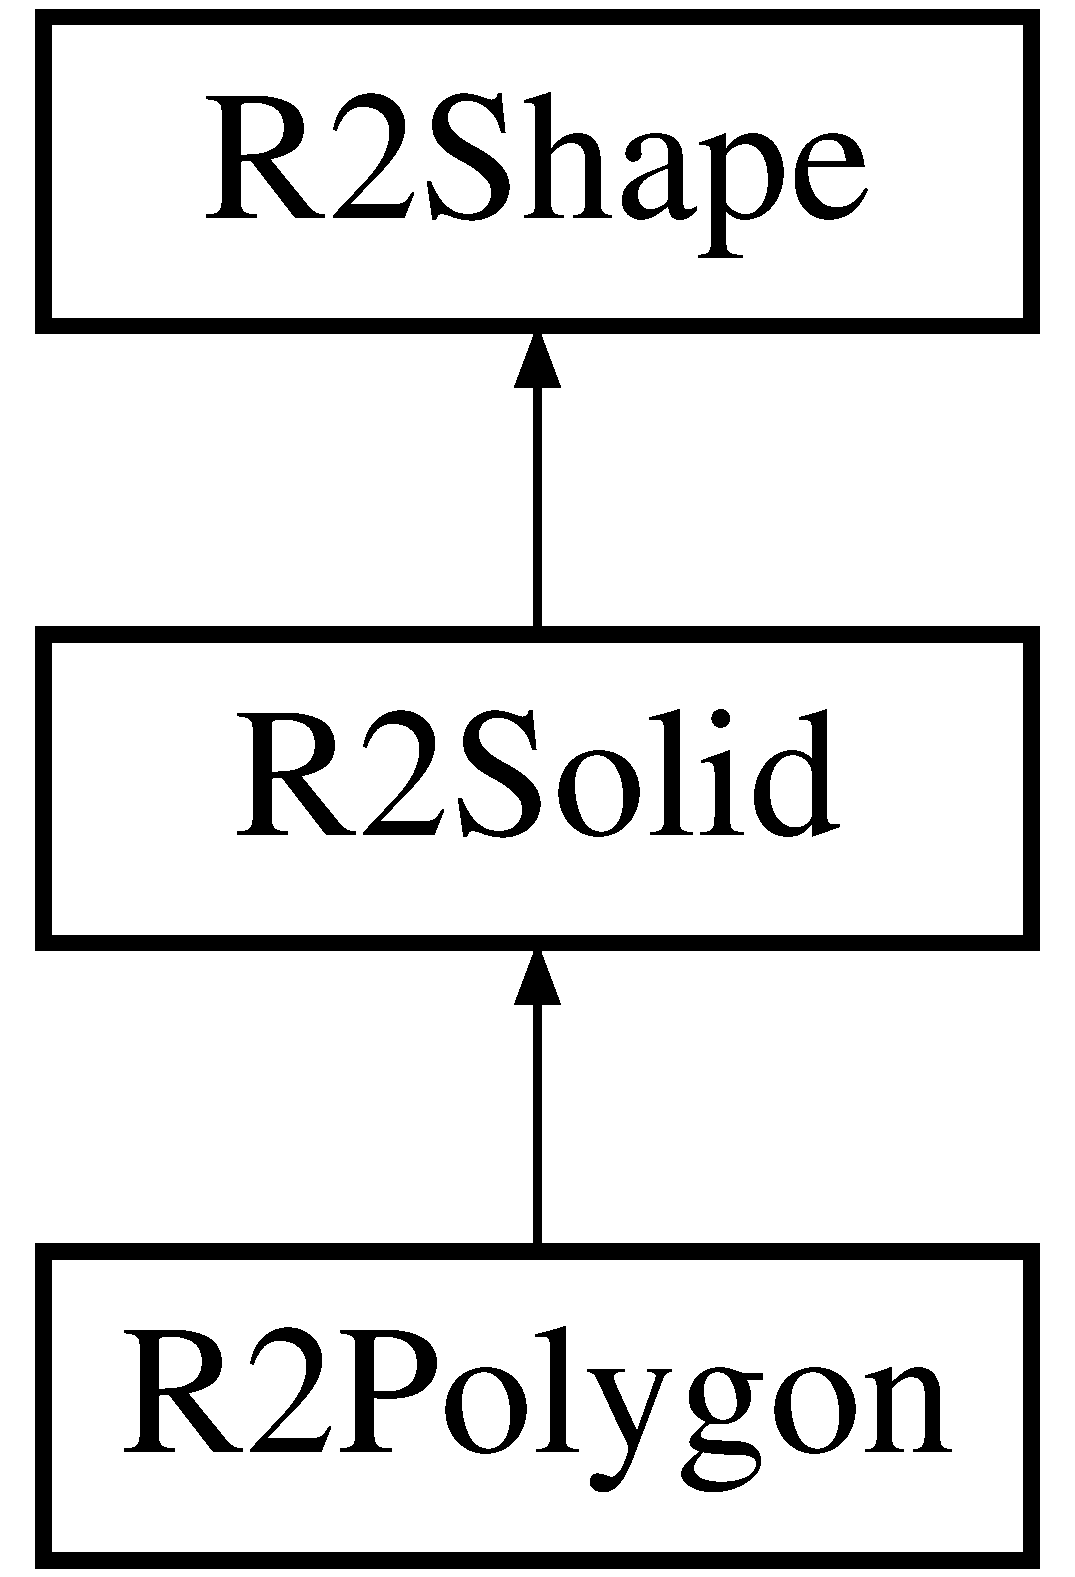
\includegraphics[height=3.000000cm]{class_r2_polygon}
\end{center}
\end{figure}
\subsection*{Public Member Functions}
\begin{DoxyCompactItemize}
\item 
{\bfseries R2\+Polygon} (const \hyperlink{class_r2_polygon}{R2\+Polygon} \&polygon)\hypertarget{class_r2_polygon_a370f204b039439ddccbf6e2e5b9fdb05}{}\label{class_r2_polygon_a370f204b039439ddccbf6e2e5b9fdb05}

\item 
{\bfseries R2\+Polygon} (const \hyperlink{class_r2_point}{R2\+Point} $\ast$points, int npoints, R\+N\+Boolean clockwise=F\+A\+L\+SE)\hypertarget{class_r2_polygon_ad90b228efd5a474c3c5cd0bd3a9c6660}{}\label{class_r2_polygon_ad90b228efd5a474c3c5cd0bd3a9c6660}

\item 
const int {\bfseries N\+Points} (void) const \hypertarget{class_r2_polygon_af30b5cbd6e7b5fa3c2cddc7c3c408de1}{}\label{class_r2_polygon_af30b5cbd6e7b5fa3c2cddc7c3c408de1}

\item 
const \hyperlink{class_r2_point}{R2\+Point} \& {\bfseries Point} (int k) const \hypertarget{class_r2_polygon_aab02de73ccf42b6c807d361599e01ada}{}\label{class_r2_polygon_aab02de73ccf42b6c807d361599e01ada}

\item 
const R\+N\+Boolean {\bfseries Is\+Empty} (void) const \hypertarget{class_r2_polygon_ac2f8c62b0cee262073c7bb0876425f4e}{}\label{class_r2_polygon_ac2f8c62b0cee262073c7bb0876425f4e}

\item 
const R\+N\+Boolean {\bfseries Is\+Finite} (void) const \hypertarget{class_r2_polygon_a3a695d9f459f2835d06b9ef7533890d7}{}\label{class_r2_polygon_a3a695d9f459f2835d06b9ef7533890d7}

\item 
const R\+N\+Boolean {\bfseries Is\+Clockwise} (void) const \hypertarget{class_r2_polygon_abe8fb8eb0284c77b7be1dece9a496030}{}\label{class_r2_polygon_abe8fb8eb0284c77b7be1dece9a496030}

\item 
const \hyperlink{class_r2_point}{R2\+Point} \& {\bfseries operator\mbox{[}$\,$\mbox{]}} (int k) const \hypertarget{class_r2_polygon_a327eb82f86be3fd677763fc5c3e0a881}{}\label{class_r2_polygon_a327eb82f86be3fd677763fc5c3e0a881}

\item 
const \hyperlink{class_r2_point}{R2\+Point} {\bfseries Closest\+Point} (const \hyperlink{class_r2_point}{R2\+Point} \&point) const \hypertarget{class_r2_polygon_af8321ce008a2f25dcec4d1641b166b01}{}\label{class_r2_polygon_af8321ce008a2f25dcec4d1641b166b01}

\item 
virtual const R\+N\+Boolean {\bfseries Is\+Point} (void) const \hypertarget{class_r2_polygon_a732c50c0fa8884a6834c47c9afa9c1ac}{}\label{class_r2_polygon_a732c50c0fa8884a6834c47c9afa9c1ac}

\item 
virtual const R\+N\+Boolean {\bfseries Is\+Linear} (void) const \hypertarget{class_r2_polygon_a9bca214e8291c33baf5e85e7dae155eb}{}\label{class_r2_polygon_a9bca214e8291c33baf5e85e7dae155eb}

\item 
virtual const R\+N\+Boolean {\bfseries Is\+Convex} (void) const \hypertarget{class_r2_polygon_a24c5e5254f7b8f1e2f61c505b6a0e013}{}\label{class_r2_polygon_a24c5e5254f7b8f1e2f61c505b6a0e013}

\item 
virtual const R\+N\+Area {\bfseries Area} (void) const \hypertarget{class_r2_polygon_ac727e2269d73113b563b5d8cd669e46a}{}\label{class_r2_polygon_ac727e2269d73113b563b5d8cd669e46a}

\item 
virtual const R\+N\+Scalar {\bfseries Convexity} (void) const \hypertarget{class_r2_polygon_ae2d49b2b0d17f0ae735e3fb220f02577}{}\label{class_r2_polygon_ae2d49b2b0d17f0ae735e3fb220f02577}

\item 
virtual const R\+N\+Length {\bfseries Perimeter} (void) const \hypertarget{class_r2_polygon_aaeeb3eeeec230c305935c45238ff1499}{}\label{class_r2_polygon_aaeeb3eeeec230c305935c45238ff1499}

\item 
virtual const \hyperlink{class_r2_point}{R2\+Point} {\bfseries Centroid} (void) const \hypertarget{class_r2_polygon_a38e12370f03169739f562f21b492790e}{}\label{class_r2_polygon_a38e12370f03169739f562f21b492790e}

\item 
virtual const \hyperlink{class_r2_shape}{R2\+Shape} \& {\bfseries B\+Shape} (void) const \hypertarget{class_r2_polygon_aa6a4e6cb57e677742b0d3c7c7e7b0a9d}{}\label{class_r2_polygon_aa6a4e6cb57e677742b0d3c7c7e7b0a9d}

\item 
virtual const \hyperlink{class_r2_box}{R2\+Box} {\bfseries B\+Box} (void) const \hypertarget{class_r2_polygon_a1b7101aecb8206e16e10dcdf8922bbd8}{}\label{class_r2_polygon_a1b7101aecb8206e16e10dcdf8922bbd8}

\item 
virtual const \hyperlink{class_r2_circle}{R2\+Circle} {\bfseries B\+Circle} (void) const \hypertarget{class_r2_polygon_a0b46763c8d38b73aea3bc8bdf36e4891}{}\label{class_r2_polygon_a0b46763c8d38b73aea3bc8bdf36e4891}

\item 
virtual const \hyperlink{class_r2_polygon}{R2\+Polygon} {\bfseries Convex\+Hull} (void) const \hypertarget{class_r2_polygon_ac5957c925e61a5b8fafd17b0466ec67a}{}\label{class_r2_polygon_ac5957c925e61a5b8fafd17b0466ec67a}

\item 
\hyperlink{class_r2_vector}{R2\+Vector} {\bfseries Normal} (int k, R\+N\+Length radius=0) const \hypertarget{class_r2_polygon_a8bdda2e17a82a39fdb2221996b9e9597}{}\label{class_r2_polygon_a8bdda2e17a82a39fdb2221996b9e9597}

\item 
\hyperlink{class_r2_line}{R2\+Line} {\bfseries Tangent} (int k, R\+N\+Length radius=0) const \hypertarget{class_r2_polygon_a9185d9625f6ac10dc24f5ace5dd065c6}{}\label{class_r2_polygon_a9185d9625f6ac10dc24f5ace5dd065c6}

\item 
R\+N\+Angle {\bfseries Interior\+Angle} (int k, R\+N\+Length radius=0) const \hypertarget{class_r2_polygon_a66db59be3f747f216229d72d9d490fd8}{}\label{class_r2_polygon_a66db59be3f747f216229d72d9d490fd8}

\item 
R\+N\+Scalar {\bfseries Curvature} (int k, R\+N\+Length radius=0) const \hypertarget{class_r2_polygon_aa94089e8c8c5d09c5aecd84246a8e06d}{}\label{class_r2_polygon_aa94089e8c8c5d09c5aecd84246a8e06d}

\item 
virtual void {\bfseries Empty} (void)\hypertarget{class_r2_polygon_ab48ad97e382c682890b611c0185dc23b}{}\label{class_r2_polygon_ab48ad97e382c682890b611c0185dc23b}

\item 
virtual void {\bfseries Clip} (const \hyperlink{class_r2_line}{R2\+Line} \&line)\hypertarget{class_r2_polygon_ae6af365707687206ac4c895f1a81f84d}{}\label{class_r2_polygon_ae6af365707687206ac4c895f1a81f84d}

\item 
virtual void {\bfseries Clip} (const \hyperlink{class_r2_box}{R2\+Box} \&\hyperlink{structbox}{box})\hypertarget{class_r2_polygon_aaf0a2b241cf4f0fd3a48878adf9f69a6}{}\label{class_r2_polygon_aaf0a2b241cf4f0fd3a48878adf9f69a6}

\item 
virtual void {\bfseries Transform} (const \hyperlink{class_r2_transformation}{R2\+Transformation} \&transformation)\hypertarget{class_r2_polygon_a378acd8a6055e8c93c37fa7c2b0f7e04}{}\label{class_r2_polygon_a378acd8a6055e8c93c37fa7c2b0f7e04}

\item 
virtual void {\bfseries Draw} (const \hyperlink{class_r_n_flags}{R2\+Draw\+Flags} draw\+\_\+flags=R2\+\_\+\+D\+E\+F\+A\+U\+L\+T\+\_\+\+D\+R\+A\+W\+\_\+\+F\+L\+A\+GS) const \hypertarget{class_r2_polygon_a687ac6d5857ce5e16b089d7077fa4db5}{}\label{class_r2_polygon_a687ac6d5857ce5e16b089d7077fa4db5}

\item 
virtual void {\bfseries Print} (F\+I\+LE $\ast$fp=stdout) const \hypertarget{class_r2_polygon_a4b390493ed26c28fbe264386c297fbf6}{}\label{class_r2_polygon_a4b390493ed26c28fbe264386c297fbf6}

\item 
virtual int {\bfseries Read\+Thera\+File} (const char $\ast$filename)\hypertarget{class_r2_polygon_a063e7d5f9fa8a579a3d98ea636662e08}{}\label{class_r2_polygon_a063e7d5f9fa8a579a3d98ea636662e08}

\end{DoxyCompactItemize}


The documentation for this class was generated from the following files\+:\begin{DoxyCompactItemize}
\item 
R2\+Shapes/R2\+Polygon.\+h\item 
R2\+Shapes/R2\+Draw.\+cpp\item 
R2\+Shapes/R2\+Polygon.\+cpp\end{DoxyCompactItemize}

\hypertarget{class_r2_ray}{}\section{R2\+Ray Class Reference}
\label{class_r2_ray}\index{R2\+Ray@{R2\+Ray}}
\subsection*{Public Member Functions}
\begin{DoxyCompactItemize}
\item 
{\bfseries R2\+Ray} (const \hyperlink{class_r2_ray}{R2\+Ray} \&ray)\hypertarget{class_r2_ray_a058a2f31541438ddcad2bb3586bb4b20}{}\label{class_r2_ray_a058a2f31541438ddcad2bb3586bb4b20}

\item 
{\bfseries R2\+Ray} (const \hyperlink{class_r2_point}{R2\+Point} \&point, const \hyperlink{class_r2_vector}{R2\+Vector} \&vector, R\+N\+Boolean normalized=F\+A\+L\+SE)\hypertarget{class_r2_ray_abff370d39ddda85006602199ad4033d6}{}\label{class_r2_ray_abff370d39ddda85006602199ad4033d6}

\item 
{\bfseries R2\+Ray} (const \hyperlink{class_r2_point}{R2\+Point} \&point1, const \hyperlink{class_r2_point}{R2\+Point} \&point2)\hypertarget{class_r2_ray_a5472afded08f4283164eac015ee9b7e3}{}\label{class_r2_ray_a5472afded08f4283164eac015ee9b7e3}

\item 
{\bfseries R2\+Ray} (R\+N\+Coord x1, R\+N\+Coord y1, R\+N\+Coord x2, R\+N\+Coord y2)\hypertarget{class_r2_ray_a14c6f626289e0a90ef2ce8a610ad0594}{}\label{class_r2_ray_a14c6f626289e0a90ef2ce8a610ad0594}

\item 
const \hyperlink{class_r2_point}{R2\+Point} \& {\bfseries Start} (void) const \hypertarget{class_r2_ray_a3d849aadfe78f5b2171983ea8a7ca20c}{}\label{class_r2_ray_a3d849aadfe78f5b2171983ea8a7ca20c}

\item 
const \hyperlink{class_r2_vector}{R2\+Vector} \& {\bfseries Vector} (void) const \hypertarget{class_r2_ray_a17985c2e7bf0d3fc9aa6ac18e6635197}{}\label{class_r2_ray_a17985c2e7bf0d3fc9aa6ac18e6635197}

\item 
const \hyperlink{class_r2_vector}{R2\+Vector} \& {\bfseries Normal} (void) const \hypertarget{class_r2_ray_a0fea465f805485d94744ca81405a82a8}{}\label{class_r2_ray_a0fea465f805485d94744ca81405a82a8}

\item 
const \hyperlink{class_r2_line}{R2\+Line} \& {\bfseries Line} (void) const \hypertarget{class_r2_ray_a38d77d185f13ecbf390b5eaf32922b4f}{}\label{class_r2_ray_a38d77d185f13ecbf390b5eaf32922b4f}

\item 
const \hyperlink{class_r2_point}{R2\+Point} {\bfseries Point} (R\+N\+Scalar t) const \hypertarget{class_r2_ray_a722370932b3d7a26b6f21f4c13184e10}{}\label{class_r2_ray_a722370932b3d7a26b6f21f4c13184e10}

\item 
const R\+N\+Scalar {\bfseries T} (const \hyperlink{class_r2_point}{R2\+Point} \&point) const \hypertarget{class_r2_ray_a6d0f777be74fa6ef3ed557091a436788}{}\label{class_r2_ray_a6d0f777be74fa6ef3ed557091a436788}

\item 
const R\+N\+Boolean {\bfseries Is\+Zero} (void) const \hypertarget{class_r2_ray_a52c2256f3ef0101ef527cce99da17542}{}\label{class_r2_ray_a52c2256f3ef0101ef527cce99da17542}

\item 
const R\+N\+Boolean {\bfseries operator==} (const \hyperlink{class_r2_ray}{R2\+Ray} \&ray) const \hypertarget{class_r2_ray_aa1c3442812cb79b5e4317926ba7ebe41}{}\label{class_r2_ray_aa1c3442812cb79b5e4317926ba7ebe41}

\item 
const R\+N\+Boolean {\bfseries operator!=} (const \hyperlink{class_r2_ray}{R2\+Ray} \&ray) const \hypertarget{class_r2_ray_ae3aa90451d20275d45e8f7a69cc670bf}{}\label{class_r2_ray_ae3aa90451d20275d45e8f7a69cc670bf}

\item 
void {\bfseries Flip} (void)\hypertarget{class_r2_ray_aa752b2be96cd80d15b01c28df3c8e850}{}\label{class_r2_ray_aa752b2be96cd80d15b01c28df3c8e850}

\item 
void {\bfseries Project} (const \hyperlink{class_r2_line}{R2\+Line} \&line)\hypertarget{class_r2_ray_aea1d71187182f874a534747063d62e5f}{}\label{class_r2_ray_aea1d71187182f874a534747063d62e5f}

\item 
void {\bfseries Mirror} (const \hyperlink{class_r2_line}{R2\+Line} \&line)\hypertarget{class_r2_ray_a2c72c0b6ec38b7b5ea91f48053d02111}{}\label{class_r2_ray_a2c72c0b6ec38b7b5ea91f48053d02111}

\item 
void {\bfseries Translate} (const \hyperlink{class_r2_vector}{R2\+Vector} \&vector)\hypertarget{class_r2_ray_a11627982fdad4034f40ccbc4f8352391}{}\label{class_r2_ray_a11627982fdad4034f40ccbc4f8352391}

\item 
void {\bfseries Reposition} (const \hyperlink{class_r2_point}{R2\+Point} \&point)\hypertarget{class_r2_ray_a043b87437606ba3f564fd60ecbad4fa8}{}\label{class_r2_ray_a043b87437606ba3f564fd60ecbad4fa8}

\item 
void {\bfseries Align} (const \hyperlink{class_r2_vector}{R2\+Vector} \&vector)\hypertarget{class_r2_ray_a96ced27e70e017184454273d74af669d}{}\label{class_r2_ray_a96ced27e70e017184454273d74af669d}

\item 
void {\bfseries Transform} (const \hyperlink{class_r2_transformation}{R2\+Transformation} \&transformation)\hypertarget{class_r2_ray_afd2b0b25f59be8d3b2c146711e17d46c}{}\label{class_r2_ray_afd2b0b25f59be8d3b2c146711e17d46c}

\item 
void {\bfseries Inverse\+Transform} (const \hyperlink{class_r2_transformation}{R2\+Transformation} \&transformation)\hypertarget{class_r2_ray_a9f1c091209e28ad4c843f075aff52889}{}\label{class_r2_ray_a9f1c091209e28ad4c843f075aff52889}

\item 
void {\bfseries Reset} (const \hyperlink{class_r2_point}{R2\+Point} \&point, const \hyperlink{class_r2_vector}{R2\+Vector} \&vector, R\+N\+Boolean normalized=F\+A\+L\+SE)\hypertarget{class_r2_ray_ae3309647b6a788cf9825127270bd89b8}{}\label{class_r2_ray_ae3309647b6a788cf9825127270bd89b8}

\item 
void {\bfseries Draw} (void) const \hypertarget{class_r2_ray_a5c6a95e861f6f14747e352bf7e88530f}{}\label{class_r2_ray_a5c6a95e861f6f14747e352bf7e88530f}

\item 
\hyperlink{class_r2_ray}{R2\+Ray} {\bfseries operator-\/} (void) const \hypertarget{class_r2_ray_a1ca8b7a3e669f479ace6da7b0b301063}{}\label{class_r2_ray_a1ca8b7a3e669f479ace6da7b0b301063}

\end{DoxyCompactItemize}


The documentation for this class was generated from the following files\+:\begin{DoxyCompactItemize}
\item 
R2\+Shapes/R2\+Ray.\+h\item 
R2\+Shapes/R2\+Draw.\+cpp\item 
R2\+Shapes/R2\+Ray.\+cpp\end{DoxyCompactItemize}

\hypertarget{class_r2_shape}{}\section{R2\+Shape Class Reference}
\label{class_r2_shape}\index{R2\+Shape@{R2\+Shape}}
Inheritance diagram for R2\+Shape\+:\begin{figure}[H]
\begin{center}
\leavevmode
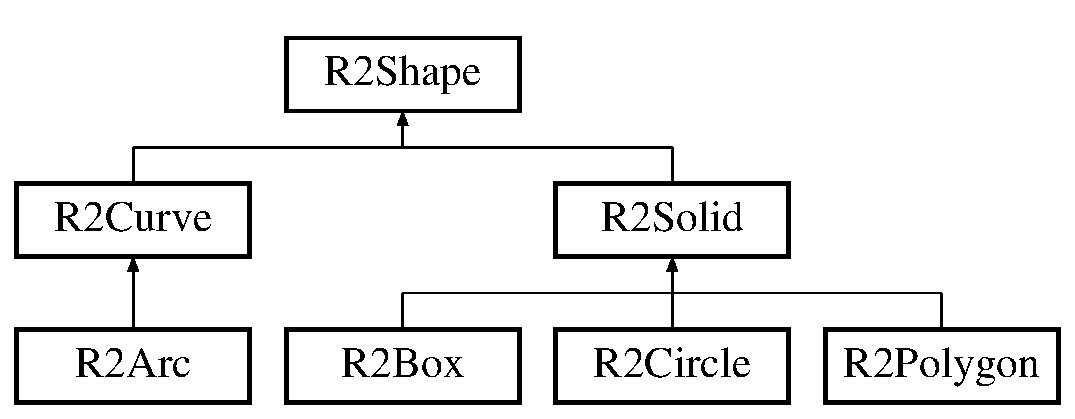
\includegraphics[height=3.000000cm]{class_r2_shape}
\end{center}
\end{figure}
\subsection*{Public Member Functions}
\begin{DoxyCompactItemize}
\item 
virtual void {\bfseries Draw} (const \hyperlink{class_r_n_flags}{R2\+Draw\+Flags} draw\+\_\+flags=R2\+\_\+\+D\+E\+F\+A\+U\+L\+T\+\_\+\+D\+R\+A\+W\+\_\+\+F\+L\+A\+GS) const  =0\hypertarget{class_r2_shape_ac3d8ebb888ca8c1ba867cd74a43a3067}{}\label{class_r2_shape_ac3d8ebb888ca8c1ba867cd74a43a3067}

\item 
void {\bfseries Outline} (void) const \hypertarget{class_r2_shape_a17b4090e3d887eb65d3d4444765ab7a1}{}\label{class_r2_shape_a17b4090e3d887eb65d3d4444765ab7a1}

\end{DoxyCompactItemize}


The documentation for this class was generated from the following file\+:\begin{DoxyCompactItemize}
\item 
R2\+Shapes/R2\+Shape.\+h\end{DoxyCompactItemize}

\hypertarget{class_r2_solid}{}\section{R2\+Solid Class Reference}
\label{class_r2_solid}\index{R2\+Solid@{R2\+Solid}}
Inheritance diagram for R2\+Solid\+:\begin{figure}[H]
\begin{center}
\leavevmode
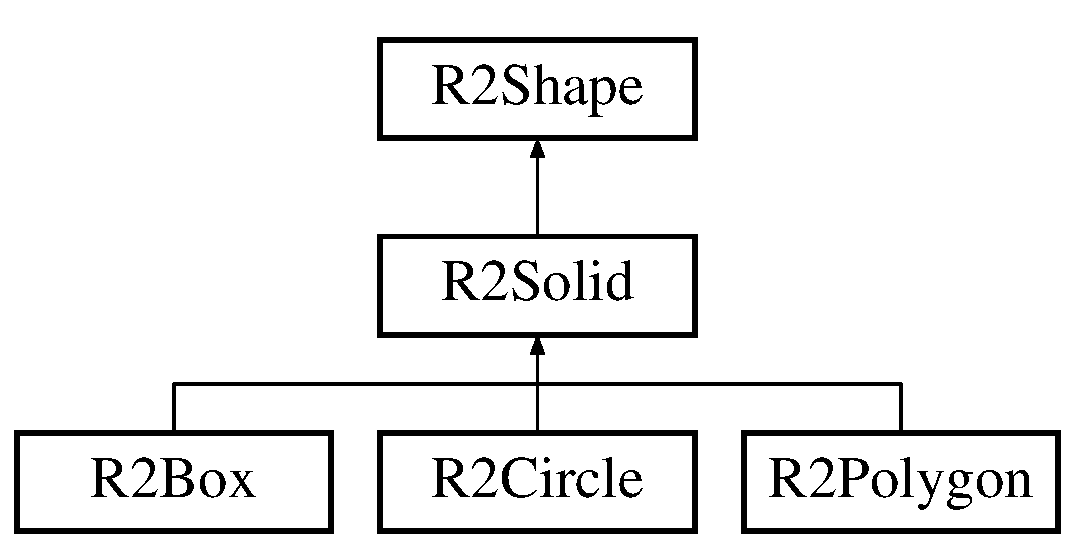
\includegraphics[height=3.000000cm]{class_r2_solid}
\end{center}
\end{figure}
\subsection*{Public Member Functions}
\begin{DoxyCompactItemize}
\item 
const R\+N\+Boolean {\bfseries Is\+Solid} (void) const \hypertarget{class_r2_solid_a52bcc096ca5bf67e4880cce983a85145}{}\label{class_r2_solid_a52bcc096ca5bf67e4880cce983a85145}

\end{DoxyCompactItemize}


The documentation for this class was generated from the following files\+:\begin{DoxyCompactItemize}
\item 
R2\+Shapes/R2\+Solid.\+h\item 
R2\+Shapes/R2\+Solid.\+cpp\end{DoxyCompactItemize}

\hypertarget{class_r2_span}{}\section{R2\+Span Class Reference}
\label{class_r2_span}\index{R2\+Span@{R2\+Span}}
\subsection*{Public Member Functions}
\begin{DoxyCompactItemize}
\item 
{\bfseries R2\+Span} (const \hyperlink{class_r2_span}{R2\+Span} \&span)\hypertarget{class_r2_span_a3c60ef06c0d0ba51b08e369367aff876}{}\label{class_r2_span_a3c60ef06c0d0ba51b08e369367aff876}

\item 
{\bfseries R2\+Span} (const \hyperlink{class_r2_point}{R2\+Point} \&point, const \hyperlink{class_r2_vector}{R2\+Vector} \&vector)\hypertarget{class_r2_span_acf0c821ea10dab859f29208385d3ee54}{}\label{class_r2_span_acf0c821ea10dab859f29208385d3ee54}

\item 
{\bfseries R2\+Span} (const \hyperlink{class_r2_point}{R2\+Point} \&point1, const \hyperlink{class_r2_point}{R2\+Point} \&point2)\hypertarget{class_r2_span_a7432fd74bb56fac6cc856b646da0f15d}{}\label{class_r2_span_a7432fd74bb56fac6cc856b646da0f15d}

\item 
{\bfseries R2\+Span} (R\+N\+Coord x1, R\+N\+Coord y1, R\+N\+Coord x2, R\+N\+Coord y2)\hypertarget{class_r2_span_ad504e54ba86d8fada5938b3bc97c3e87}{}\label{class_r2_span_ad504e54ba86d8fada5938b3bc97c3e87}

\item 
const \hyperlink{class_r2_point}{R2\+Point} \& {\bfseries Start} (void) const \hypertarget{class_r2_span_ae88dadb214e6fbfd8f9e02801c548bb6}{}\label{class_r2_span_ae88dadb214e6fbfd8f9e02801c548bb6}

\item 
const \hyperlink{class_r2_point}{R2\+Point} \& {\bfseries End} (void) const \hypertarget{class_r2_span_a35092f972b2963f3f7f98af5a29c7a4c}{}\label{class_r2_span_a35092f972b2963f3f7f98af5a29c7a4c}

\item 
const \hyperlink{class_r2_vector}{R2\+Vector} \& {\bfseries Vector} (void) const \hypertarget{class_r2_span_ae3f1b43d779448c2ad4eb033506760ac}{}\label{class_r2_span_ae3f1b43d779448c2ad4eb033506760ac}

\item 
const \hyperlink{class_r2_vector}{R2\+Vector} \& {\bfseries Normal} (void) const \hypertarget{class_r2_span_a481642f8778e123384cc14db2ffe4145}{}\label{class_r2_span_a481642f8778e123384cc14db2ffe4145}

\item 
const \hyperlink{class_r2_point}{R2\+Point} {\bfseries Point} (int k) const \hypertarget{class_r2_span_ab6f9f6e9e95852676072efb4f94fac45}{}\label{class_r2_span_ab6f9f6e9e95852676072efb4f94fac45}

\item 
const \hyperlink{class_r2_point}{R2\+Point} {\bfseries Point} (R\+N\+Scalar t) const \hypertarget{class_r2_span_ae88e7e33bd5860590bb4717d28cc3eae}{}\label{class_r2_span_ae88e7e33bd5860590bb4717d28cc3eae}

\item 
const \hyperlink{class_r2_point}{R2\+Point} \& {\bfseries operator\mbox{[}$\,$\mbox{]}} (int k) const \hypertarget{class_r2_span_af63e910c1ab5f9e177c4227eae413c99}{}\label{class_r2_span_af63e910c1ab5f9e177c4227eae413c99}

\item 
const \hyperlink{class_r2_ray}{R2\+Ray} \& {\bfseries Ray} (void) const \hypertarget{class_r2_span_ad6c53967f91585fd409065bcd56f7ebd}{}\label{class_r2_span_ad6c53967f91585fd409065bcd56f7ebd}

\item 
const \hyperlink{class_r2_line}{R2\+Line} \& {\bfseries Line} (void) const \hypertarget{class_r2_span_aeab7c8842b838cab4192ccbba194183f}{}\label{class_r2_span_aeab7c8842b838cab4192ccbba194183f}

\item 
const \hyperlink{class_r2_point}{R2\+Point} {\bfseries Midpoint} (void) const \hypertarget{class_r2_span_a0adeb97a390a68a3b660face5ee54e0e}{}\label{class_r2_span_a0adeb97a390a68a3b660face5ee54e0e}

\item 
const \hyperlink{class_r2_point}{R2\+Point} {\bfseries Centroid} (void) const \hypertarget{class_r2_span_a144edd0a9476eb63edf3fdc3a7be301e}{}\label{class_r2_span_a144edd0a9476eb63edf3fdc3a7be301e}

\item 
const R\+N\+Length {\bfseries Length} (void) const \hypertarget{class_r2_span_aef2f5da746c7c8c830dfc1bf911c0bd9}{}\label{class_r2_span_aef2f5da746c7c8c830dfc1bf911c0bd9}

\item 
const R\+N\+Scalar {\bfseries T} (const \hyperlink{class_r2_point}{R2\+Point} \&point) const \hypertarget{class_r2_span_ab5f96e4bce51b67bdd0f04827edb6bc3}{}\label{class_r2_span_ab5f96e4bce51b67bdd0f04827edb6bc3}

\item 
const R\+N\+Boolean {\bfseries Is\+Point} (void) const \hypertarget{class_r2_span_a68ca8488236b27dbea15d5098cc1c4c5}{}\label{class_r2_span_a68ca8488236b27dbea15d5098cc1c4c5}

\item 
const R\+N\+Boolean {\bfseries operator==} (const \hyperlink{class_r2_span}{R2\+Span} \&span) const \hypertarget{class_r2_span_adc2a35b295b0b6fb828117d56bf7f3b7}{}\label{class_r2_span_adc2a35b295b0b6fb828117d56bf7f3b7}

\item 
const R\+N\+Boolean {\bfseries operator!=} (const \hyperlink{class_r2_span}{R2\+Span} \&span) const \hypertarget{class_r2_span_afcf9de48f8ec3dbadabdb8ba12a2845f}{}\label{class_r2_span_afcf9de48f8ec3dbadabdb8ba12a2845f}

\item 
const \hyperlink{class_r2_box}{R2\+Box} {\bfseries B\+Box} (void) const \hypertarget{class_r2_span_a480178f2b56db05406063a33cb01cf83}{}\label{class_r2_span_a480178f2b56db05406063a33cb01cf83}

\item 
const \hyperlink{class_r2_circle}{R2\+Circle} {\bfseries B\+Circle} (void) const \hypertarget{class_r2_span_a4edb9446e09abbf147caa97e4c4a289e}{}\label{class_r2_span_a4edb9446e09abbf147caa97e4c4a289e}

\item 
void {\bfseries Flip} (void)\hypertarget{class_r2_span_a0938a01442cbb5d355a42f219a193cde}{}\label{class_r2_span_a0938a01442cbb5d355a42f219a193cde}

\item 
void {\bfseries Project} (const \hyperlink{class_r2_line}{R2\+Line} \&line)\hypertarget{class_r2_span_a82b432085df4c048db092f2b01fe27e1}{}\label{class_r2_span_a82b432085df4c048db092f2b01fe27e1}

\item 
void {\bfseries Mirror} (const \hyperlink{class_r2_line}{R2\+Line} \&line)\hypertarget{class_r2_span_ae4c1aff9c394a92e598e59445635468a}{}\label{class_r2_span_ae4c1aff9c394a92e598e59445635468a}

\item 
void {\bfseries Translate} (const \hyperlink{class_r2_vector}{R2\+Vector} \&vector)\hypertarget{class_r2_span_aa5d8eabb8cb03f5085d04afbf30e9122}{}\label{class_r2_span_aa5d8eabb8cb03f5085d04afbf30e9122}

\item 
void {\bfseries Reposition} (int k, const \hyperlink{class_r2_point}{R2\+Point} \&point)\hypertarget{class_r2_span_acd88dbf022abc40eebc8f01be9212f8b}{}\label{class_r2_span_acd88dbf022abc40eebc8f01be9212f8b}

\item 
void {\bfseries Align} (const \hyperlink{class_r2_vector}{R2\+Vector} \&vector)\hypertarget{class_r2_span_a7f236a19c3115d31fcbbd44357ebec0a}{}\label{class_r2_span_a7f236a19c3115d31fcbbd44357ebec0a}

\item 
void {\bfseries Transform} (const \hyperlink{class_r2_transformation}{R2\+Transformation} \&transformation)\hypertarget{class_r2_span_a11439f85eeacccb75f43660346f0b758}{}\label{class_r2_span_a11439f85eeacccb75f43660346f0b758}

\item 
void {\bfseries Inverse\+Transform} (const \hyperlink{class_r2_transformation}{R2\+Transformation} \&transformation)\hypertarget{class_r2_span_a86927e2eb43fc03ba5d4dada46475cef}{}\label{class_r2_span_a86927e2eb43fc03ba5d4dada46475cef}

\item 
void {\bfseries Reset} (const \hyperlink{class_r2_point}{R2\+Point} \&point1, const \hyperlink{class_r2_point}{R2\+Point} \&point2)\hypertarget{class_r2_span_ab03cf7bb188bb9eb7bd69a2d27eb5fb9}{}\label{class_r2_span_ab03cf7bb188bb9eb7bd69a2d27eb5fb9}

\item 
R\+N\+Class\+ID {\bfseries Clip} (const \hyperlink{class_r2_line}{R2\+Line} \&line)\hypertarget{class_r2_span_a48e3ed556c7432b8ad500847ad15b266}{}\label{class_r2_span_a48e3ed556c7432b8ad500847ad15b266}

\item 
void {\bfseries Draw} (void) const \hypertarget{class_r2_span_abd8c5b78ed40a072e29acd89a6d0d73a}{}\label{class_r2_span_abd8c5b78ed40a072e29acd89a6d0d73a}

\item 
\hyperlink{class_r2_span}{R2\+Span} {\bfseries operator-\/} (void) const \hypertarget{class_r2_span_a35985c4394199ef239a5ba7a85ae99ce}{}\label{class_r2_span_a35985c4394199ef239a5ba7a85ae99ce}

\end{DoxyCompactItemize}


The documentation for this class was generated from the following files\+:\begin{DoxyCompactItemize}
\item 
R2\+Shapes/R2\+Span.\+h\item 
R2\+Shapes/R2\+Draw.\+cpp\item 
R2\+Shapes/R2\+Span.\+cpp\end{DoxyCompactItemize}

\hypertarget{class_r2_texture}{}\section{R2\+Texture Class Reference}
\label{class_r2_texture}\index{R2\+Texture@{R2\+Texture}}
\subsection*{Public Member Functions}
\begin{DoxyCompactItemize}
\item 
{\bfseries R2\+Texture} (const \hyperlink{class_r2_texture}{R2\+Texture} \&texture)\hypertarget{class_r2_texture_aa0d837b618bacd079b5f017106290de3}{}\label{class_r2_texture_aa0d837b618bacd079b5f017106290de3}

\item 
{\bfseries R2\+Texture} (const \hyperlink{class_r2_image}{R2\+Image} $\ast$image, R2\+Texture\+Wrap s\+\_\+wrap=R2\+\_\+\+R\+E\+P\+E\+A\+T\+\_\+\+T\+E\+X\+T\+U\+R\+E\+\_\+\+W\+R\+AP, R2\+Texture\+Wrap t\+\_\+wrap=R2\+\_\+\+R\+E\+P\+E\+A\+T\+\_\+\+T\+E\+X\+T\+U\+R\+E\+\_\+\+W\+R\+AP, R2\+Texture\+Filter min\+\_\+filter=R2\+\_\+\+L\+I\+N\+E\+A\+R\+\_\+\+T\+E\+X\+T\+U\+R\+E\+\_\+\+F\+I\+L\+T\+ER, R2\+Texture\+Filter mag\+\_\+filter=R2\+\_\+\+L\+I\+N\+E\+A\+R\+\_\+\+T\+E\+X\+T\+U\+R\+E\+\_\+\+F\+I\+L\+T\+ER, R2\+Texture\+Blend blend=R2\+\_\+\+M\+O\+D\+U\+L\+A\+T\+E\+\_\+\+T\+E\+X\+T\+U\+R\+E\+\_\+\+B\+L\+E\+ND)\hypertarget{class_r2_texture_a8407f16675357b4e01d1581615286399}{}\label{class_r2_texture_a8407f16675357b4e01d1581615286399}

\item 
{\bfseries R2\+Texture} (const char $\ast$filename, R2\+Texture\+Wrap s\+\_\+wrap=R2\+\_\+\+C\+L\+A\+M\+P\+\_\+\+T\+E\+X\+T\+U\+R\+E\+\_\+\+W\+R\+AP, R2\+Texture\+Wrap t\+\_\+wrap=R2\+\_\+\+C\+L\+A\+M\+P\+\_\+\+T\+E\+X\+T\+U\+R\+E\+\_\+\+W\+R\+AP, R2\+Texture\+Filter min\+\_\+filter=R2\+\_\+\+L\+I\+N\+E\+A\+R\+\_\+\+T\+E\+X\+T\+U\+R\+E\+\_\+\+F\+I\+L\+T\+ER, R2\+Texture\+Filter mag\+\_\+filter=R2\+\_\+\+L\+I\+N\+E\+A\+R\+\_\+\+T\+E\+X\+T\+U\+R\+E\+\_\+\+F\+I\+L\+T\+ER, R2\+Texture\+Blend blend=R2\+\_\+\+M\+O\+D\+U\+L\+A\+T\+E\+\_\+\+T\+E\+X\+T\+U\+R\+E\+\_\+\+B\+L\+E\+ND)\hypertarget{class_r2_texture_a970f811d9fb50a87158c26ae08f268c5}{}\label{class_r2_texture_a970f811d9fb50a87158c26ae08f268c5}

\item 
const \hyperlink{class_r2_image}{R2\+Image} $\ast$ {\bfseries Image} (void) const \hypertarget{class_r2_texture_a1436a86c2b43b1ee864f81f6ab7d203b}{}\label{class_r2_texture_a1436a86c2b43b1ee864f81f6ab7d203b}

\item 
const R2\+Texture\+Wrap {\bfseries S\+Wrap} (void) const \hypertarget{class_r2_texture_a162db0fa79e5158ab4aec75926585fc9}{}\label{class_r2_texture_a162db0fa79e5158ab4aec75926585fc9}

\item 
const R2\+Texture\+Wrap {\bfseries T\+Wrap} (void) const \hypertarget{class_r2_texture_a906d713825c171372c546925e0f8d241}{}\label{class_r2_texture_a906d713825c171372c546925e0f8d241}

\item 
const R2\+Texture\+Filter {\bfseries Min\+Filter} (void) const \hypertarget{class_r2_texture_a9b5fcf65df338ddfde5d99c9580b158a}{}\label{class_r2_texture_a9b5fcf65df338ddfde5d99c9580b158a}

\item 
const R2\+Texture\+Filter {\bfseries Mag\+Filter} (void) const \hypertarget{class_r2_texture_a39fae65a85f544284812b8204a0ae505}{}\label{class_r2_texture_a39fae65a85f544284812b8204a0ae505}

\item 
const R2\+Texture\+Blend {\bfseries Blend} (void) const \hypertarget{class_r2_texture_a6fb54dd13e6e4bd49a071c9f36bae03a}{}\label{class_r2_texture_a6fb54dd13e6e4bd49a071c9f36bae03a}

\item 
const R\+N\+Boolean {\bfseries Is\+Transparent} (void) const \hypertarget{class_r2_texture_a6f0774412a87f8a0747a13c9417b4fb8}{}\label{class_r2_texture_a6f0774412a87f8a0747a13c9417b4fb8}

\item 
const R\+N\+Boolean {\bfseries Is\+Loaded} (void) const \hypertarget{class_r2_texture_a3b6963f2fae27baed735d5df8e570ca1}{}\label{class_r2_texture_a3b6963f2fae27baed735d5df8e570ca1}

\item 
const \hyperlink{class_r_n_flags}{R\+N\+Flags} {\bfseries Flags} (void) const \hypertarget{class_r2_texture_a3798e0fabbd81f81cd4915a6cc65261e}{}\label{class_r2_texture_a3798e0fabbd81f81cd4915a6cc65261e}

\item 
const int {\bfseries ID} (void) const \hypertarget{class_r2_texture_a065bf34d710f168009fbb9dd73be5ac8}{}\label{class_r2_texture_a065bf34d710f168009fbb9dd73be5ac8}

\item 
void {\bfseries Set\+Image} (const \hyperlink{class_r2_image}{R2\+Image} $\ast$image)\hypertarget{class_r2_texture_a25168ce976af52de3ff33aefd923d5e0}{}\label{class_r2_texture_a25168ce976af52de3ff33aefd923d5e0}

\item 
void {\bfseries Load} (void) const \hypertarget{class_r2_texture_a6f253a9604eb6241f560e325826cb90f}{}\label{class_r2_texture_a6f253a9604eb6241f560e325826cb90f}

\item 
void {\bfseries Unload} (void) const \hypertarget{class_r2_texture_aeff5b175732a5cd05c49e4438deab688}{}\label{class_r2_texture_aeff5b175732a5cd05c49e4438deab688}

\item 
void {\bfseries Draw} (R\+N\+Boolean force=F\+A\+L\+SE) const \hypertarget{class_r2_texture_a2da983c68a5bca30e69b10849b784270}{}\label{class_r2_texture_a2da983c68a5bca30e69b10849b784270}

\end{DoxyCompactItemize}
\subsection*{Protected Member Functions}
\begin{DoxyCompactItemize}
\item 
void {\bfseries Update} (void)\hypertarget{class_r2_texture_adae649e592b44388a09c4a4820fccac9}{}\label{class_r2_texture_adae649e592b44388a09c4a4820fccac9}

\item 
void {\bfseries Update\+Flags} (const \hyperlink{class_r_n_flags}{R\+N\+Flags} flags)\hypertarget{class_r2_texture_a65b5cdb0d3cc51bb7aef7bfd0a1b4315}{}\label{class_r2_texture_a65b5cdb0d3cc51bb7aef7bfd0a1b4315}

\end{DoxyCompactItemize}


The documentation for this class was generated from the following files\+:\begin{DoxyCompactItemize}
\item 
R3\+Graphics/R2\+Texture.\+h\item 
R3\+Graphics/R2\+Texture.\+cpp\end{DoxyCompactItemize}

\hypertarget{class_r2_transformation}{}\section{R2\+Transformation Class Reference}
\label{class_r2_transformation}\index{R2\+Transformation@{R2\+Transformation}}
Inheritance diagram for R2\+Transformation\+:\begin{figure}[H]
\begin{center}
\leavevmode
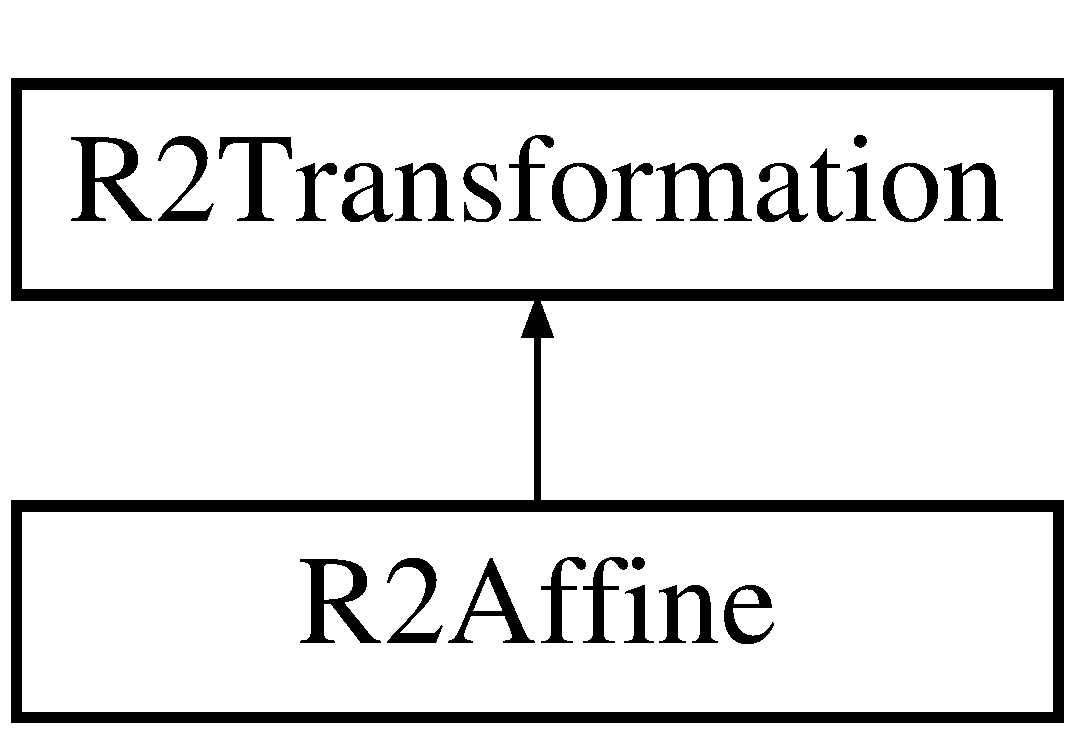
\includegraphics[height=2.000000cm]{class_r2_transformation}
\end{center}
\end{figure}
\subsection*{Public Member Functions}
\begin{DoxyCompactItemize}
\item 
virtual const R\+N\+Boolean {\bfseries Is\+Mirrored} (void) const \hypertarget{class_r2_transformation_ae8e3ad90301ac17af1047679763e0ed2}{}\label{class_r2_transformation_ae8e3ad90301ac17af1047679763e0ed2}

\item 
virtual const R\+N\+Boolean {\bfseries Is\+Linear} (void) const \hypertarget{class_r2_transformation_ad61d41bf45d3da00a31b45ee0dfef022}{}\label{class_r2_transformation_ad61d41bf45d3da00a31b45ee0dfef022}

\item 
virtual const R\+N\+Boolean {\bfseries Is\+Affine} (void) const \hypertarget{class_r2_transformation_ab0f3b893e49bd3534820a14fefd1903a}{}\label{class_r2_transformation_ab0f3b893e49bd3534820a14fefd1903a}

\item 
virtual const R\+N\+Boolean {\bfseries Is\+Isotropic} (void) const \hypertarget{class_r2_transformation_a906661967eb5c6b71112cc51866600bc}{}\label{class_r2_transformation_a906661967eb5c6b71112cc51866600bc}

\item 
virtual void {\bfseries Apply} (\hyperlink{class_r2_vector}{R2\+Vector} \&vector) const  =0\hypertarget{class_r2_transformation_afc2a2082277dcebaf261b67f1e62e2e3}{}\label{class_r2_transformation_afc2a2082277dcebaf261b67f1e62e2e3}

\item 
virtual void {\bfseries Apply} (\hyperlink{class_r2_point}{R2\+Point} \&point) const  =0\hypertarget{class_r2_transformation_aac9b0f354e8fb6f94b3be2efeb72c967}{}\label{class_r2_transformation_aac9b0f354e8fb6f94b3be2efeb72c967}

\item 
virtual void {\bfseries Apply} (\hyperlink{class_r2_transformation}{R2\+Transformation} \&transformation) const  =0\hypertarget{class_r2_transformation_adb15b45eb1a3ab9a5eda20514136a0bc}{}\label{class_r2_transformation_adb15b45eb1a3ab9a5eda20514136a0bc}

\item 
virtual void {\bfseries Apply} (\hyperlink{class_r2_affine}{R2\+Affine} \&affine) const  =0\hypertarget{class_r2_transformation_a01b79abf84878148f5630b6893a516e6}{}\label{class_r2_transformation_a01b79abf84878148f5630b6893a516e6}

\item 
virtual void {\bfseries Apply\+Inverse} (\hyperlink{class_r2_vector}{R2\+Vector} \&vector) const  =0\hypertarget{class_r2_transformation_a41519d44b1b34827b274980e3042bd17}{}\label{class_r2_transformation_a41519d44b1b34827b274980e3042bd17}

\item 
virtual void {\bfseries Apply\+Inverse} (\hyperlink{class_r2_point}{R2\+Point} \&point) const  =0\hypertarget{class_r2_transformation_a5553808b3c32d479c811e72154fde2a0}{}\label{class_r2_transformation_a5553808b3c32d479c811e72154fde2a0}

\item 
virtual void {\bfseries Apply\+Inverse} (\hyperlink{class_r2_transformation}{R2\+Transformation} \&transformation) const  =0\hypertarget{class_r2_transformation_a0fe799238277dce506ff042e5b960179}{}\label{class_r2_transformation_a0fe799238277dce506ff042e5b960179}

\item 
virtual void {\bfseries Apply\+Inverse} (\hyperlink{class_r2_affine}{R2\+Affine} \&affine) const  =0\hypertarget{class_r2_transformation_ace4b452ab83e23940069099bcb9cd82e}{}\label{class_r2_transformation_ace4b452ab83e23940069099bcb9cd82e}

\item 
virtual void {\bfseries Reset} (const \hyperlink{class_r2_transformation}{R2\+Transformation} \&transformation)=0\hypertarget{class_r2_transformation_a2642ff67f5dccb9b24248839d0531701}{}\label{class_r2_transformation_a2642ff67f5dccb9b24248839d0531701}

\item 
virtual void {\bfseries Transform} (const \hyperlink{class_r2_transformation}{R2\+Transformation} \&transformation)=0\hypertarget{class_r2_transformation_a387a684d4d558ce4c09f18c5d15f3789}{}\label{class_r2_transformation_a387a684d4d558ce4c09f18c5d15f3789}

\item 
virtual void {\bfseries Inverse\+Transform} (const \hyperlink{class_r2_transformation}{R2\+Transformation} \&transformation)=0\hypertarget{class_r2_transformation_a1799be1bca0a4031b94a4ef345167798}{}\label{class_r2_transformation_a1799be1bca0a4031b94a4ef345167798}

\item 
virtual void {\bfseries Load} (void) const  =0\hypertarget{class_r2_transformation_aea112a53f758a251bf4ad2dc5cfcb0f7}{}\label{class_r2_transformation_aea112a53f758a251bf4ad2dc5cfcb0f7}

\item 
virtual void {\bfseries Draw} (void) const  =0\hypertarget{class_r2_transformation_aa795402b979a0a221977eacfe89f6f44}{}\label{class_r2_transformation_aa795402b979a0a221977eacfe89f6f44}

\item 
virtual void {\bfseries Push} (void) const  =0\hypertarget{class_r2_transformation_afdf5880fc64bdb5f4216fc3272ff0a65}{}\label{class_r2_transformation_afdf5880fc64bdb5f4216fc3272ff0a65}

\item 
virtual void {\bfseries Pop} (void) const  =0\hypertarget{class_r2_transformation_a796c2fb8ab519e2ff4ae461408fc079b}{}\label{class_r2_transformation_a796c2fb8ab519e2ff4ae461408fc079b}

\end{DoxyCompactItemize}


The documentation for this class was generated from the following files\+:\begin{DoxyCompactItemize}
\item 
R2\+Shapes/R2\+Xform.\+h\item 
R2\+Shapes/R2\+Xform.\+cpp\end{DoxyCompactItemize}

\hypertarget{class_r2_vector}{}\section{R2\+Vector Class Reference}
\label{class_r2_vector}\index{R2\+Vector@{R2\+Vector}}
\subsection*{Public Member Functions}
\begin{DoxyCompactItemize}
\item 
{\bfseries R2\+Vector} (const \hyperlink{class_r2_vector}{R2\+Vector} \&vector)\hypertarget{class_r2_vector_ada6a42ce5c022332c0674da5f6f20a2c}{}\label{class_r2_vector_ada6a42ce5c022332c0674da5f6f20a2c}

\item 
{\bfseries R2\+Vector} (R\+N\+Coord x, R\+N\+Coord y)\hypertarget{class_r2_vector_a138e7ca86d26ec80dd19a7624ac3d63b}{}\label{class_r2_vector_a138e7ca86d26ec80dd19a7624ac3d63b}

\item 
{\bfseries R2\+Vector} (const R\+N\+Coord array\mbox{[}2\mbox{]})\hypertarget{class_r2_vector_abc3804c917b81b6d5f09a0da2cb0e28c}{}\label{class_r2_vector_abc3804c917b81b6d5f09a0da2cb0e28c}

\item 
{\bfseries R2\+Vector} (R\+N\+Angle angle)\hypertarget{class_r2_vector_a9f34915d0490da4a1df816b5cddc4b4e}{}\label{class_r2_vector_a9f34915d0490da4a1df816b5cddc4b4e}

\item 
const R\+N\+Coord {\bfseries X} (void) const \hypertarget{class_r2_vector_a5deccbf33352b96658a3e345ff14f8b6}{}\label{class_r2_vector_a5deccbf33352b96658a3e345ff14f8b6}

\item 
const R\+N\+Coord {\bfseries Y} (void) const \hypertarget{class_r2_vector_a4705367026d4c2175135de603e994062}{}\label{class_r2_vector_a4705367026d4c2175135de603e994062}

\item 
const R\+N\+Coord {\bfseries Coord} (R\+N\+Dimension dim) const \hypertarget{class_r2_vector_ab732cc7f541273f464fdeae77896f6d3}{}\label{class_r2_vector_ab732cc7f541273f464fdeae77896f6d3}

\item 
const R\+N\+Coord {\bfseries operator\mbox{[}$\,$\mbox{]}} (R\+N\+Dimension dim) const \hypertarget{class_r2_vector_a0dc6bebe700e66508d899d5ba5f23fee}{}\label{class_r2_vector_a0dc6bebe700e66508d899d5ba5f23fee}

\item 
const R\+N\+Coord $\ast$ {\bfseries Coords} (void) const \hypertarget{class_r2_vector_a95adba8bc76bc32e8a4be12967f2559a}{}\label{class_r2_vector_a95adba8bc76bc32e8a4be12967f2559a}

\item 
const R\+N\+Boolean {\bfseries Is\+Zero} (void) const \hypertarget{class_r2_vector_a52b9331e43fc57454e1af1fe09f3eae3}{}\label{class_r2_vector_a52b9331e43fc57454e1af1fe09f3eae3}

\item 
const R\+N\+Boolean {\bfseries Is\+Finite} (void) const \hypertarget{class_r2_vector_a7c908472b6ff6ce1fbd9e137ec1b51b7}{}\label{class_r2_vector_a7c908472b6ff6ce1fbd9e137ec1b51b7}

\item 
const R\+N\+Boolean {\bfseries Is\+Normalized} (void) const \hypertarget{class_r2_vector_aa108f7e49e841253e56f2d4486901f02}{}\label{class_r2_vector_aa108f7e49e841253e56f2d4486901f02}

\item 
const R\+N\+Length {\bfseries Length} (void) const \hypertarget{class_r2_vector_a05671fd6152d4a865cdd20b61741aea0}{}\label{class_r2_vector_a05671fd6152d4a865cdd20b61741aea0}

\item 
const R\+N\+Angle {\bfseries Angle} (void) const \hypertarget{class_r2_vector_a49470f895c29b35963198afb72f90198}{}\label{class_r2_vector_a49470f895c29b35963198afb72f90198}

\item 
const \hyperlink{class_r2_point}{R2\+Point} {\bfseries Point} (void) const \hypertarget{class_r2_vector_a0f8faba6a5f968d4535091c3bf46c0bf}{}\label{class_r2_vector_a0f8faba6a5f968d4535091c3bf46c0bf}

\item 
const R\+N\+Quadrant {\bfseries Quadrant} (void) const \hypertarget{class_r2_vector_a7a8291cc042cd77290452db3d5359d45}{}\label{class_r2_vector_a7a8291cc042cd77290452db3d5359d45}

\item 
const R\+N\+Dimension {\bfseries Max\+Dimension} (void) const \hypertarget{class_r2_vector_a7910e7c22089e9df746d6ad9ebfb1340}{}\label{class_r2_vector_a7910e7c22089e9df746d6ad9ebfb1340}

\item 
const R\+N\+Boolean {\bfseries operator==} (const \hyperlink{class_r2_vector}{R2\+Vector} \&vector) const \hypertarget{class_r2_vector_af29622d25f41ce999766016ec01eba83}{}\label{class_r2_vector_af29622d25f41ce999766016ec01eba83}

\item 
const R\+N\+Boolean {\bfseries operator!=} (const \hyperlink{class_r2_vector}{R2\+Vector} \&vector) const \hypertarget{class_r2_vector_a205c168855985bed9a3043125182bc55}{}\label{class_r2_vector_a205c168855985bed9a3043125182bc55}

\item 
const R\+N\+Scalar {\bfseries Dot} (const \hyperlink{class_r2_vector}{R2\+Vector} \&vector) const \hypertarget{class_r2_vector_ae0653778982303095e3fd26f05edf13f}{}\label{class_r2_vector_ae0653778982303095e3fd26f05edf13f}

\item 
const R\+N\+Scalar {\bfseries Cross} (const \hyperlink{class_r2_vector}{R2\+Vector} \&vector) const \hypertarget{class_r2_vector_a6f08d12daea47fd773e2e1bbc46337a0}{}\label{class_r2_vector_a6f08d12daea47fd773e2e1bbc46337a0}

\item 
void {\bfseries X} (R\+N\+Coord x)\hypertarget{class_r2_vector_a87394d2eeb7cf20a8b68e4e1ca723c29}{}\label{class_r2_vector_a87394d2eeb7cf20a8b68e4e1ca723c29}

\item 
void {\bfseries Y} (R\+N\+Coord y)\hypertarget{class_r2_vector_a575b034f3830d6c00671a1e671ccced0}{}\label{class_r2_vector_a575b034f3830d6c00671a1e671ccced0}

\item 
void {\bfseries Set\+Coord} (R\+N\+Dimension dim, R\+N\+Coord coord)\hypertarget{class_r2_vector_a15e90da3fede4e9c6b57df03898f5c54}{}\label{class_r2_vector_a15e90da3fede4e9c6b57df03898f5c54}

\item 
void {\bfseries Flip} (void)\hypertarget{class_r2_vector_a15eda2f45f9511c514758cb7cade1d76}{}\label{class_r2_vector_a15eda2f45f9511c514758cb7cade1d76}

\item 
void {\bfseries Normalize} (void)\hypertarget{class_r2_vector_a05815045f5d8827acc70a6098aa10930}{}\label{class_r2_vector_a05815045f5d8827acc70a6098aa10930}

\item 
void {\bfseries Scale} (R\+N\+Scalar a)\hypertarget{class_r2_vector_a6edda42f20bfd5006c0ceee9923c6482}{}\label{class_r2_vector_a6edda42f20bfd5006c0ceee9923c6482}

\item 
void {\bfseries Rotate} (R\+N\+Angle theta)\hypertarget{class_r2_vector_a9f5c0f90ac7c631213305bf9a3056f6a}{}\label{class_r2_vector_a9f5c0f90ac7c631213305bf9a3056f6a}

\item 
void {\bfseries Project} (const \hyperlink{class_r2_vector}{R2\+Vector} \&vector)\hypertarget{class_r2_vector_a5e4376742632b36733e3bfe87421d382}{}\label{class_r2_vector_a5e4376742632b36733e3bfe87421d382}

\item 
void {\bfseries Mirror} (const \hyperlink{class_r2_line}{R2\+Line} \&line)\hypertarget{class_r2_vector_a630c6d2f03bb60b579d78e0231f25e0a}{}\label{class_r2_vector_a630c6d2f03bb60b579d78e0231f25e0a}

\item 
void {\bfseries Transform} (const \hyperlink{class_r2_transformation}{R2\+Transformation} \&transformation)\hypertarget{class_r2_vector_abe359376ecebb26fa14fdb38170d8149}{}\label{class_r2_vector_abe359376ecebb26fa14fdb38170d8149}

\item 
void {\bfseries Inverse\+Transform} (const \hyperlink{class_r2_transformation}{R2\+Transformation} \&transformation)\hypertarget{class_r2_vector_a8ccfbe1acb83f1088e0c6cf432917903}{}\label{class_r2_vector_a8ccfbe1acb83f1088e0c6cf432917903}

\item 
void {\bfseries Reset} (R\+N\+Coord x, R\+N\+Coord y)\hypertarget{class_r2_vector_a5e93c1548324067601788d5d39edfbbe}{}\label{class_r2_vector_a5e93c1548324067601788d5d39edfbbe}

\item 
void {\bfseries Draw} (void) const \hypertarget{class_r2_vector_ac9ef6f2c7251f3be6766aedf400158b2}{}\label{class_r2_vector_ac9ef6f2c7251f3be6766aedf400158b2}

\item 
\hyperlink{class_r2_vector}{R2\+Vector} \& {\bfseries operator=} (const \hyperlink{class_r2_vector}{R2\+Vector} \&vector)\hypertarget{class_r2_vector_ad4df4303a924dcc4098f69928f61c091}{}\label{class_r2_vector_ad4df4303a924dcc4098f69928f61c091}

\item 
\hyperlink{class_r2_vector}{R2\+Vector} \& {\bfseries operator+=} (const \hyperlink{class_r2_vector}{R2\+Vector} \&vector)\hypertarget{class_r2_vector_a0f9afd0a7f748405058a1740a218c541}{}\label{class_r2_vector_a0f9afd0a7f748405058a1740a218c541}

\item 
\hyperlink{class_r2_vector}{R2\+Vector} \& {\bfseries operator-\/=} (const \hyperlink{class_r2_vector}{R2\+Vector} \&vector)\hypertarget{class_r2_vector_af22b058fb6a661c7a858c8d9459af979}{}\label{class_r2_vector_af22b058fb6a661c7a858c8d9459af979}

\item 
\hyperlink{class_r2_vector}{R2\+Vector} \& {\bfseries operator$\ast$=} (const R\+N\+Scalar a)\hypertarget{class_r2_vector_ae44e661d65faa3517c06967f4e41c7b3}{}\label{class_r2_vector_ae44e661d65faa3517c06967f4e41c7b3}

\item 
\hyperlink{class_r2_vector}{R2\+Vector} \& {\bfseries operator$\ast$=} (const \hyperlink{class_r2_vector}{R2\+Vector} \&vector)\hypertarget{class_r2_vector_af9c5325fe980cfc24b64e3a4ce15fb01}{}\label{class_r2_vector_af9c5325fe980cfc24b64e3a4ce15fb01}

\item 
\hyperlink{class_r2_vector}{R2\+Vector} \& {\bfseries operator$\ast$=} (const \hyperlink{class_r3_matrix}{R3\+Matrix} \&matrix)\hypertarget{class_r2_vector_af75f22818f4531d863ceb4887291fb96}{}\label{class_r2_vector_af75f22818f4531d863ceb4887291fb96}

\item 
\hyperlink{class_r2_vector}{R2\+Vector} \& {\bfseries operator/=} (const R\+N\+Scalar a)\hypertarget{class_r2_vector_a7ea909f2879fd0a489359e2d36a00a34}{}\label{class_r2_vector_a7ea909f2879fd0a489359e2d36a00a34}

\item 
\hyperlink{class_r2_vector}{R2\+Vector} \& {\bfseries operator/=} (const \hyperlink{class_r2_vector}{R2\+Vector} \&vector)\hypertarget{class_r2_vector_a9694d85cccdb3f1500101adc18b70051}{}\label{class_r2_vector_a9694d85cccdb3f1500101adc18b70051}

\item 
R\+N\+Coord \& {\bfseries operator\mbox{[}$\,$\mbox{]}} (R\+N\+Dimension dim)\hypertarget{class_r2_vector_a32c7c22c3286de4e84f358316cf2e7bb}{}\label{class_r2_vector_a32c7c22c3286de4e84f358316cf2e7bb}

\end{DoxyCompactItemize}
\subsection*{Friends}
\begin{DoxyCompactItemize}
\item 
\hyperlink{class_r2_vector}{R2\+Vector} {\bfseries operator+} (const \hyperlink{class_r2_vector}{R2\+Vector} \&vector)\hypertarget{class_r2_vector_a423a3dc6059364fa119b9ef4c4500ae7}{}\label{class_r2_vector_a423a3dc6059364fa119b9ef4c4500ae7}

\item 
\hyperlink{class_r2_vector}{R2\+Vector} {\bfseries operator-\/} (const \hyperlink{class_r2_vector}{R2\+Vector} \&vector)\hypertarget{class_r2_vector_a462a9d162fe41976ead654702ae66017}{}\label{class_r2_vector_a462a9d162fe41976ead654702ae66017}

\item 
\hyperlink{class_r2_vector}{R2\+Vector} {\bfseries operator+} (const \hyperlink{class_r2_vector}{R2\+Vector} \&vector1, const \hyperlink{class_r2_vector}{R2\+Vector} \&vector2)\hypertarget{class_r2_vector_ab6caca78d0c35a4bfb9889df81e42f6c}{}\label{class_r2_vector_ab6caca78d0c35a4bfb9889df81e42f6c}

\item 
\hyperlink{class_r2_vector}{R2\+Vector} {\bfseries operator-\/} (const \hyperlink{class_r2_vector}{R2\+Vector} \&vector1, const \hyperlink{class_r2_vector}{R2\+Vector} \&vector2)\hypertarget{class_r2_vector_a3cbb3a606ba7bc8f570fbfc09f2e022a}{}\label{class_r2_vector_a3cbb3a606ba7bc8f570fbfc09f2e022a}

\item 
\hyperlink{class_r2_vector}{R2\+Vector} {\bfseries operator$\ast$} (const \hyperlink{class_r2_vector}{R2\+Vector} \&vector1, const \hyperlink{class_r2_vector}{R2\+Vector} \&vector2)\hypertarget{class_r2_vector_a9fa6329ad3f2b8b6e56a264c9c6d8fd2}{}\label{class_r2_vector_a9fa6329ad3f2b8b6e56a264c9c6d8fd2}

\item 
\hyperlink{class_r2_vector}{R2\+Vector} {\bfseries operator$\ast$} (const \hyperlink{class_r2_vector}{R2\+Vector} \&vector, const R\+N\+Scalar a)\hypertarget{class_r2_vector_acb46cbf083fffe9f0fc4b64873b92c81}{}\label{class_r2_vector_acb46cbf083fffe9f0fc4b64873b92c81}

\item 
\hyperlink{class_r2_vector}{R2\+Vector} {\bfseries operator$\ast$} (const R\+N\+Scalar a, const \hyperlink{class_r2_vector}{R2\+Vector} \&vector)\hypertarget{class_r2_vector_a87b38b6afcd8ca1191645b7dcf58fdfd}{}\label{class_r2_vector_a87b38b6afcd8ca1191645b7dcf58fdfd}

\item 
\hyperlink{class_r2_vector}{R2\+Vector} {\bfseries operator$\ast$} (const \hyperlink{class_r2_vector}{R2\+Vector} \&vector, const \hyperlink{class_r3_matrix}{R3\+Matrix} \&m)\hypertarget{class_r2_vector_a4766dd8eed3f662a2dd9e6c778412dc1}{}\label{class_r2_vector_a4766dd8eed3f662a2dd9e6c778412dc1}

\item 
\hyperlink{class_r2_vector}{R2\+Vector} {\bfseries operator/} (const \hyperlink{class_r2_vector}{R2\+Vector} \&vector1, const \hyperlink{class_r2_vector}{R2\+Vector} \&vector2)\hypertarget{class_r2_vector_a60b7391a208d40547391f784d56c829a}{}\label{class_r2_vector_a60b7391a208d40547391f784d56c829a}

\item 
\hyperlink{class_r2_vector}{R2\+Vector} {\bfseries operator/} (const \hyperlink{class_r2_vector}{R2\+Vector} \&vector, const R\+N\+Scalar a)\hypertarget{class_r2_vector_ab7aaea5cfb8669ff074b5722b569f64d}{}\label{class_r2_vector_ab7aaea5cfb8669ff074b5722b569f64d}

\item 
R\+N\+Scalar {\bfseries operator\%} (const \hyperlink{class_r2_vector}{R2\+Vector} \&vector1, const \hyperlink{class_r2_vector}{R2\+Vector} \&vector2)\hypertarget{class_r2_vector_a03c9a4bbce9ee09be5bb8bf2bb05c2a1}{}\label{class_r2_vector_a03c9a4bbce9ee09be5bb8bf2bb05c2a1}

\end{DoxyCompactItemize}


The documentation for this class was generated from the following files\+:\begin{DoxyCompactItemize}
\item 
R2\+Shapes/R2\+Vector.\+h\item 
R2\+Shapes/R2\+Draw.\+cpp\item 
R2\+Shapes/R2\+Vector.\+cpp\end{DoxyCompactItemize}

\hypertarget{class_r2_viewport}{}\section{R2\+Viewport Class Reference}
\label{class_r2_viewport}\index{R2\+Viewport@{R2\+Viewport}}
\subsection*{Public Member Functions}
\begin{DoxyCompactItemize}
\item 
{\bfseries R2\+Viewport} (int xmin, int ymin, int width, int height)\hypertarget{class_r2_viewport_a28653acc6bfb680cb42032d1772d37e2}{}\label{class_r2_viewport_a28653acc6bfb680cb42032d1772d37e2}

\item 
const int {\bfseries X\+Min} (void) const \hypertarget{class_r2_viewport_ae53df8000d7292123beb9d324ecebb30}{}\label{class_r2_viewport_ae53df8000d7292123beb9d324ecebb30}

\item 
const int {\bfseries Y\+Min} (void) const \hypertarget{class_r2_viewport_acc08aff80f738660de20a5001418c39b}{}\label{class_r2_viewport_acc08aff80f738660de20a5001418c39b}

\item 
const int {\bfseries X\+Max} (void) const \hypertarget{class_r2_viewport_abc82ed4efa767dafbdff455da6ae5872}{}\label{class_r2_viewport_abc82ed4efa767dafbdff455da6ae5872}

\item 
const int {\bfseries Y\+Max} (void) const \hypertarget{class_r2_viewport_ad33160c9a2d6599b97334cf8b60dd4e1}{}\label{class_r2_viewport_ad33160c9a2d6599b97334cf8b60dd4e1}

\item 
const int {\bfseries Width} (void) const \hypertarget{class_r2_viewport_a081b008b346e2c1fb669b439aec07947}{}\label{class_r2_viewport_a081b008b346e2c1fb669b439aec07947}

\item 
const int {\bfseries Height} (void) const \hypertarget{class_r2_viewport_aab1f41debf3a23e63f34fd20abc53747}{}\label{class_r2_viewport_aab1f41debf3a23e63f34fd20abc53747}

\item 
const int {\bfseries X\+Center} (void) const \hypertarget{class_r2_viewport_adb2f114783ec31091819670d7b7ac35b}{}\label{class_r2_viewport_adb2f114783ec31091819670d7b7ac35b}

\item 
const int {\bfseries Y\+Center} (void) const \hypertarget{class_r2_viewport_a6d6be65c7219855ff691dc29fe262179}{}\label{class_r2_viewport_a6d6be65c7219855ff691dc29fe262179}

\item 
const int {\bfseries Area} (void) const \hypertarget{class_r2_viewport_a20f15da612067b1862eaa57603fc6ee3}{}\label{class_r2_viewport_a20f15da612067b1862eaa57603fc6ee3}

\item 
const \hyperlink{class_r2_box}{R2\+Box} {\bfseries B\+Box} (void) const \hypertarget{class_r2_viewport_a44eae848c3b4fd3025bfdc4ac1ee0a3a}{}\label{class_r2_viewport_a44eae848c3b4fd3025bfdc4ac1ee0a3a}

\item 
const R\+N\+Boolean {\bfseries operator==} (const \hyperlink{class_r2_viewport}{R2\+Viewport} \&viewport) const \hypertarget{class_r2_viewport_a46f10ebb4a2178ba7ef8c40e895037af}{}\label{class_r2_viewport_a46f10ebb4a2178ba7ef8c40e895037af}

\item 
const R\+N\+Boolean {\bfseries operator!=} (const \hyperlink{class_r2_viewport}{R2\+Viewport} \&viewport) const \hypertarget{class_r2_viewport_ae16d1b84cba6c504d7cf7433bf84367f}{}\label{class_r2_viewport_ae16d1b84cba6c504d7cf7433bf84367f}

\item 
void {\bfseries Move} (int xmin, int ymin)\hypertarget{class_r2_viewport_ad318211597314045fe3a58006ba4019c}{}\label{class_r2_viewport_ad318211597314045fe3a58006ba4019c}

\item 
void {\bfseries Resize} (int width, int height)\hypertarget{class_r2_viewport_a97dcbf74df41aeb3e0d7f682f3cb6c43}{}\label{class_r2_viewport_a97dcbf74df41aeb3e0d7f682f3cb6c43}

\item 
void {\bfseries Resize} (int xmin, int ymin, int width, int height)\hypertarget{class_r2_viewport_a8dca87e845620ff7152581a006b42567}{}\label{class_r2_viewport_a8dca87e845620ff7152581a006b42567}

\item 
void {\bfseries Load} (void) const \hypertarget{class_r2_viewport_ad4cddf1bb82f7f7ee2a39513dd4d0ac7}{}\label{class_r2_viewport_ad4cddf1bb82f7f7ee2a39513dd4d0ac7}

\end{DoxyCompactItemize}


The documentation for this class was generated from the following files\+:\begin{DoxyCompactItemize}
\item 
R3\+Graphics/R2\+Viewport.\+h\item 
R3\+Graphics/R2\+Viewport.\+cpp\end{DoxyCompactItemize}

\hypertarget{class_r3_affine}{}\section{R3\+Affine Class Reference}
\label{class_r3_affine}\index{R3\+Affine@{R3\+Affine}}
Inheritance diagram for R3\+Affine\+:\begin{figure}[H]
\begin{center}
\leavevmode
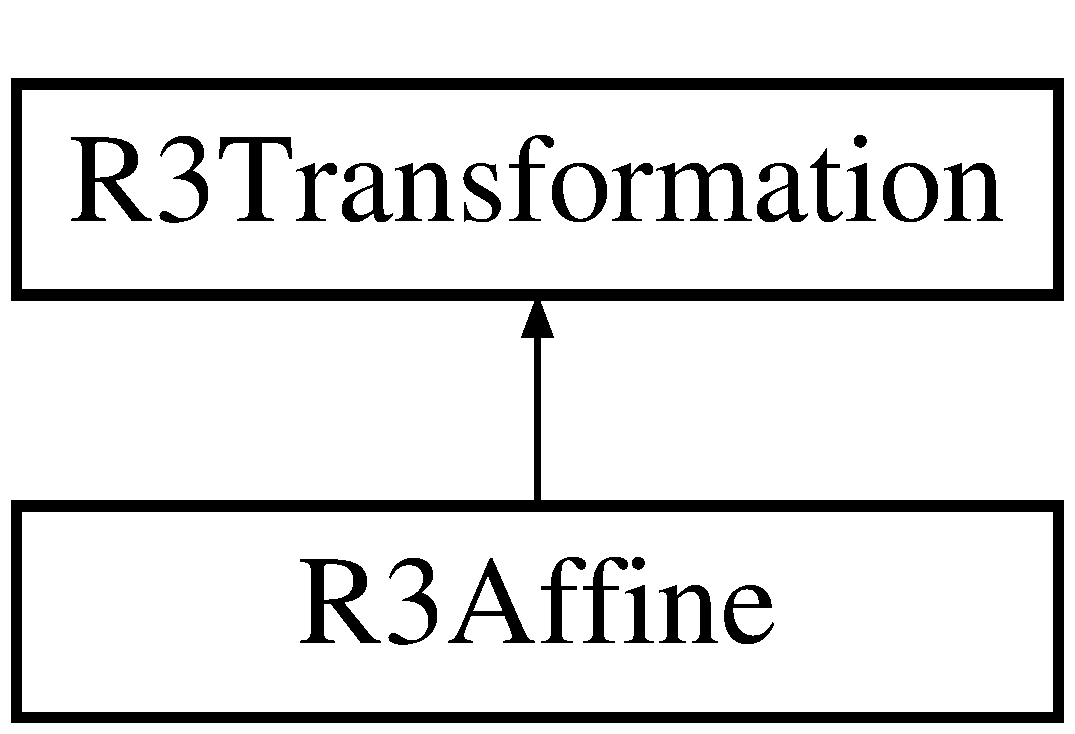
\includegraphics[height=2.000000cm]{class_r3_affine}
\end{center}
\end{figure}
\subsection*{Public Member Functions}
\begin{DoxyCompactItemize}
\item 
{\bfseries R3\+Affine} (const \hyperlink{class_r4_matrix}{R4\+Matrix} \&matrix, R\+N\+Boolean mirror=0)\hypertarget{class_r3_affine_a9ac526b0ec685cc87b1c8830ad70fb95}{}\label{class_r3_affine_a9ac526b0ec685cc87b1c8830ad70fb95}

\item 
const \hyperlink{class_r4_matrix}{R4\+Matrix} \& {\bfseries Matrix} (void) const \hypertarget{class_r3_affine_a4b378314112cd75774f172d5eafb90a2}{}\label{class_r3_affine_a4b378314112cd75774f172d5eafb90a2}

\item 
const \hyperlink{class_r4_matrix}{R4\+Matrix} \& {\bfseries Inverse\+Matrix} (void) const \hypertarget{class_r3_affine_a3bddcfc3ee4ca90ef33e831734db62ba}{}\label{class_r3_affine_a3bddcfc3ee4ca90ef33e831734db62ba}

\item 
const R\+N\+Boolean {\bfseries Is\+Identity} (void) const \hypertarget{class_r3_affine_a81b8c40d5d3b6a93329f793b76db6859}{}\label{class_r3_affine_a81b8c40d5d3b6a93329f793b76db6859}

\item 
const R\+N\+Boolean {\bfseries Is\+Mirrored} (void) const \hypertarget{class_r3_affine_a6c0afaeb7c4b23c78262d0c89333d65b}{}\label{class_r3_affine_a6c0afaeb7c4b23c78262d0c89333d65b}

\item 
const R\+N\+Boolean {\bfseries Is\+Affine} (void) const \hypertarget{class_r3_affine_acc96270e8d5d18b6df01465327f532f1}{}\label{class_r3_affine_acc96270e8d5d18b6df01465327f532f1}

\item 
const R\+N\+Boolean {\bfseries Is\+Isotropic} (void) const \hypertarget{class_r3_affine_a2d12662c6cb51b86a0617341405fead9}{}\label{class_r3_affine_a2d12662c6cb51b86a0617341405fead9}

\item 
const R\+N\+Boolean {\bfseries Has\+Translation} (void) const \hypertarget{class_r3_affine_a6d27c40cb353173059873a6b23db5b6a}{}\label{class_r3_affine_a6d27c40cb353173059873a6b23db5b6a}

\item 
const R\+N\+Boolean {\bfseries Has\+Scale} (void) const \hypertarget{class_r3_affine_a268202be11d7d142421c20afe71f4986}{}\label{class_r3_affine_a268202be11d7d142421c20afe71f4986}

\item 
const R\+N\+Boolean {\bfseries Has\+Rotation} (void) const \hypertarget{class_r3_affine_a74506b838d04073affcdb4f2c3f5c544}{}\label{class_r3_affine_a74506b838d04073affcdb4f2c3f5c544}

\item 
const R\+N\+Boolean {\bfseries Has\+Mirror} (void) const \hypertarget{class_r3_affine_ab8670281671f71ddc8b5a5e77691bf16}{}\label{class_r3_affine_ab8670281671f71ddc8b5a5e77691bf16}

\item 
const \hyperlink{class_r3_affine}{R3\+Affine} {\bfseries Inverse} (void) const \hypertarget{class_r3_affine_a83b2f8ceac524a0944f8cf82ae312c89}{}\label{class_r3_affine_a83b2f8ceac524a0944f8cf82ae312c89}

\item 
const R\+N\+Boolean {\bfseries operator==} (const \hyperlink{class_r3_affine}{R3\+Affine} \&affine) const \hypertarget{class_r3_affine_a7858f1f15123b2d2d4cb5ba4d91f938f}{}\label{class_r3_affine_a7858f1f15123b2d2d4cb5ba4d91f938f}

\item 
const R\+N\+Boolean {\bfseries operator!=} (const \hyperlink{class_r3_affine}{R3\+Affine} \&affine) const \hypertarget{class_r3_affine_ae8d64376960133e8da6dbdc3f8097dda}{}\label{class_r3_affine_ae8d64376960133e8da6dbdc3f8097dda}

\item 
void {\bfseries Apply} (\hyperlink{class_r3_vector}{R3\+Vector} \&vector) const \hypertarget{class_r3_affine_a4e20260ca95f0565bbf0f39a4ccbb30f}{}\label{class_r3_affine_a4e20260ca95f0565bbf0f39a4ccbb30f}

\item 
void {\bfseries Apply} (\hyperlink{class_r3_point}{R3\+Point} \&point) const \hypertarget{class_r3_affine_ac99658f6d9833ac41a4d21c612dbe755}{}\label{class_r3_affine_ac99658f6d9833ac41a4d21c612dbe755}

\item 
void {\bfseries Apply} (\hyperlink{class_r3_transformation}{R3\+Transformation} \&transformation) const \hypertarget{class_r3_affine_a3e9db7a1073974bfbdf1d65632523288}{}\label{class_r3_affine_a3e9db7a1073974bfbdf1d65632523288}

\item 
void {\bfseries Apply} (\hyperlink{class_r3_affine}{R3\+Affine} \&affine) const \hypertarget{class_r3_affine_a05a31b85cacd826855bcafe29972448f}{}\label{class_r3_affine_a05a31b85cacd826855bcafe29972448f}

\item 
void {\bfseries Apply\+Inverse} (\hyperlink{class_r3_vector}{R3\+Vector} \&vector) const \hypertarget{class_r3_affine_a16fc8de7007337c4976a5dc713cfb43b}{}\label{class_r3_affine_a16fc8de7007337c4976a5dc713cfb43b}

\item 
void {\bfseries Apply\+Inverse} (\hyperlink{class_r3_point}{R3\+Point} \&point) const \hypertarget{class_r3_affine_abff1abd39987570b6c7fc83f6c0f6a30}{}\label{class_r3_affine_abff1abd39987570b6c7fc83f6c0f6a30}

\item 
void {\bfseries Apply\+Inverse} (\hyperlink{class_r3_transformation}{R3\+Transformation} \&transformation) const \hypertarget{class_r3_affine_a9bb65026888ac5e99b28fd263bbfcaa5}{}\label{class_r3_affine_a9bb65026888ac5e99b28fd263bbfcaa5}

\item 
void {\bfseries Apply\+Inverse} (\hyperlink{class_r3_affine}{R3\+Affine} \&affine) const \hypertarget{class_r3_affine_ab369797f3b1afec85aacee31f50e6c23}{}\label{class_r3_affine_ab369797f3b1afec85aacee31f50e6c23}

\item 
void {\bfseries Apply\+Inverse\+Transpose} (\hyperlink{class_r3_vector}{R3\+Vector} \&vector) const \hypertarget{class_r3_affine_a7eabc4b0c0c8589f03a86f1694905521}{}\label{class_r3_affine_a7eabc4b0c0c8589f03a86f1694905521}

\item 
void {\bfseries Apply\+Transpose} (\hyperlink{class_r3_vector}{R3\+Vector} \&vector) const \hypertarget{class_r3_affine_a7c7ff9a4db2a72f5a3e6835a1a7a463f}{}\label{class_r3_affine_a7c7ff9a4db2a72f5a3e6835a1a7a463f}

\item 
void {\bfseries Invert} (void)\hypertarget{class_r3_affine_aed96b66fb075c823347832424bbe19c8}{}\label{class_r3_affine_aed96b66fb075c823347832424bbe19c8}

\item 
void {\bfseries Mirror} (void)\hypertarget{class_r3_affine_ac9aa9ea7283efb89df643b6a9fe5e75d}{}\label{class_r3_affine_ac9aa9ea7283efb89df643b6a9fe5e75d}

\item 
void {\bfseries X\+Mirror} (void)\hypertarget{class_r3_affine_a4d23c4ee8a5af5f29658a3418eef5d3d}{}\label{class_r3_affine_a4d23c4ee8a5af5f29658a3418eef5d3d}

\item 
void {\bfseries Y\+Mirror} (void)\hypertarget{class_r3_affine_aac741a2db84153c782a81723a9afa13f}{}\label{class_r3_affine_aac741a2db84153c782a81723a9afa13f}

\item 
void {\bfseries Z\+Mirror} (void)\hypertarget{class_r3_affine_ad496305c4367e6524110458f8afeeee6}{}\label{class_r3_affine_ad496305c4367e6524110458f8afeeee6}

\item 
void {\bfseries Mirror} (R\+N\+Axis axis)\hypertarget{class_r3_affine_a74245bd59ed5de0a11c78ded8b548299}{}\label{class_r3_affine_a74245bd59ed5de0a11c78ded8b548299}

\item 
void {\bfseries Mirror} (const \hyperlink{class_r3_plane}{R3\+Plane} \&plane)\hypertarget{class_r3_affine_a3206a6e8079e9f66193017627c2c9041}{}\label{class_r3_affine_a3206a6e8079e9f66193017627c2c9041}

\item 
void {\bfseries X\+Translate} (R\+N\+Scalar offset)\hypertarget{class_r3_affine_a61562d891e42536575d9cec92c6e7845}{}\label{class_r3_affine_a61562d891e42536575d9cec92c6e7845}

\item 
void {\bfseries Y\+Translate} (R\+N\+Scalar offset)\hypertarget{class_r3_affine_ae6fa0231cc4bface61148a2bcd7fecd7}{}\label{class_r3_affine_ae6fa0231cc4bface61148a2bcd7fecd7}

\item 
void {\bfseries Z\+Translate} (R\+N\+Scalar offset)\hypertarget{class_r3_affine_af90791329ecd24378304e13d8f50b0ac}{}\label{class_r3_affine_af90791329ecd24378304e13d8f50b0ac}

\item 
void {\bfseries Translate} (R\+N\+Scalar offset)\hypertarget{class_r3_affine_a6278a5d31a94ba06974e577605e8aafa}{}\label{class_r3_affine_a6278a5d31a94ba06974e577605e8aafa}

\item 
void {\bfseries Translate} (R\+N\+Axis axis, R\+N\+Scalar offset)\hypertarget{class_r3_affine_a2541ce2c6211ae9d138042ce1f6ff0af}{}\label{class_r3_affine_a2541ce2c6211ae9d138042ce1f6ff0af}

\item 
void {\bfseries Translate} (const \hyperlink{class_r3_vector}{R3\+Vector} \&offset)\hypertarget{class_r3_affine_ad7e08915c335d218bbfedaf6bf51c482}{}\label{class_r3_affine_ad7e08915c335d218bbfedaf6bf51c482}

\item 
void {\bfseries X\+Scale} (R\+N\+Scalar scale)\hypertarget{class_r3_affine_ac3bfeaabf58c646f3f31fdc6549b995c}{}\label{class_r3_affine_ac3bfeaabf58c646f3f31fdc6549b995c}

\item 
void {\bfseries Y\+Scale} (R\+N\+Scalar scale)\hypertarget{class_r3_affine_a4b9ac77969baedbae2678df5a953c01b}{}\label{class_r3_affine_a4b9ac77969baedbae2678df5a953c01b}

\item 
void {\bfseries Z\+Scale} (R\+N\+Scalar scale)\hypertarget{class_r3_affine_a576bc98c90a28aafc7abd0640b13ba42}{}\label{class_r3_affine_a576bc98c90a28aafc7abd0640b13ba42}

\item 
void {\bfseries Scale} (R\+N\+Scalar scale)\hypertarget{class_r3_affine_ad141fea29c141a8122390a38a50cf4ad}{}\label{class_r3_affine_ad141fea29c141a8122390a38a50cf4ad}

\item 
void {\bfseries Scale} (R\+N\+Axis axis, R\+N\+Scalar scale)\hypertarget{class_r3_affine_a0dbf0268adc9a2d84df1eed9f3f4dfa9}{}\label{class_r3_affine_a0dbf0268adc9a2d84df1eed9f3f4dfa9}

\item 
void {\bfseries Scale} (const \hyperlink{class_r3_vector}{R3\+Vector} \&scale)\hypertarget{class_r3_affine_a6890f28c86625a3913e141bcdfa51c02}{}\label{class_r3_affine_a6890f28c86625a3913e141bcdfa51c02}

\item 
void {\bfseries X\+Rotate} (R\+N\+Angle radians)\hypertarget{class_r3_affine_a5d09945febfc22742429b6f931ff5701}{}\label{class_r3_affine_a5d09945febfc22742429b6f931ff5701}

\item 
void {\bfseries Y\+Rotate} (R\+N\+Angle radians)\hypertarget{class_r3_affine_afa7efa31ccfe53b11f4c2a59a8c493ea}{}\label{class_r3_affine_afa7efa31ccfe53b11f4c2a59a8c493ea}

\item 
void {\bfseries Z\+Rotate} (R\+N\+Angle radians)\hypertarget{class_r3_affine_a30227412eb45a79f1ad62bfdde696a60}{}\label{class_r3_affine_a30227412eb45a79f1ad62bfdde696a60}

\item 
void {\bfseries Rotate} (const \hyperlink{class_r3_vector}{R3\+Vector} \&radians)\hypertarget{class_r3_affine_a416257ce5f316a73e66cb807a49403bb}{}\label{class_r3_affine_a416257ce5f316a73e66cb807a49403bb}

\item 
void {\bfseries Rotate} (R\+N\+Axis axis, R\+N\+Angle radians)\hypertarget{class_r3_affine_a38df894e7c4a150674de657c756931f3}{}\label{class_r3_affine_a38df894e7c4a150674de657c756931f3}

\item 
void {\bfseries Rotate} (const \hyperlink{class_r3_vector}{R3\+Vector} \&vector, R\+N\+Angle radians)\hypertarget{class_r3_affine_aaa59fbf247fcddbfda6d62b94cd7fe90}{}\label{class_r3_affine_aaa59fbf247fcddbfda6d62b94cd7fe90}

\item 
void {\bfseries Rotate} (const \hyperlink{class_r3_vector}{R3\+Vector} \&from, const \hyperlink{class_r3_vector}{R3\+Vector} \&to)\hypertarget{class_r3_affine_a949bba0e1024a953f247897ed1662e38}{}\label{class_r3_affine_a949bba0e1024a953f247897ed1662e38}

\item 
void {\bfseries Rotate} (const \hyperlink{class_r3_quaternion}{R3\+Quaternion} \&quaternion)\hypertarget{class_r3_affine_a161d1a09fb2788f988f1845a54ae3414}{}\label{class_r3_affine_a161d1a09fb2788f988f1845a54ae3414}

\item 
void {\bfseries Transform} (const \hyperlink{class_r3_transformation}{R3\+Transformation} \&transformation)\hypertarget{class_r3_affine_a46ab8262e4988d11797be68d4b1b2852}{}\label{class_r3_affine_a46ab8262e4988d11797be68d4b1b2852}

\item 
void {\bfseries Transform} (const \hyperlink{class_r3_affine}{R3\+Affine} \&affine)\hypertarget{class_r3_affine_a5cfef547dc6c12e77eca85844b39d4c2}{}\label{class_r3_affine_a5cfef547dc6c12e77eca85844b39d4c2}

\item 
void {\bfseries Inverse\+Transform} (const \hyperlink{class_r3_transformation}{R3\+Transformation} \&transformation)\hypertarget{class_r3_affine_adf00889b4e39e0062b672bab1f5b594e}{}\label{class_r3_affine_adf00889b4e39e0062b672bab1f5b594e}

\item 
void {\bfseries Inverse\+Transform} (const \hyperlink{class_r3_affine}{R3\+Affine} \&affine)\hypertarget{class_r3_affine_a869c6829406ef32fc502676005fbcc7b}{}\label{class_r3_affine_a869c6829406ef32fc502676005fbcc7b}

\item 
void {\bfseries Reset} (const \hyperlink{class_r3_transformation}{R3\+Transformation} \&transformation)\hypertarget{class_r3_affine_a4c10f6219605516e6d032896c245934c}{}\label{class_r3_affine_a4c10f6219605516e6d032896c245934c}

\item 
void {\bfseries Reset} (const \hyperlink{class_r4_matrix}{R4\+Matrix} \&matrix, R\+N\+Boolean mirror=0)\hypertarget{class_r3_affine_a8ca545eed97aa3282220d61b29fbdbea}{}\label{class_r3_affine_a8ca545eed97aa3282220d61b29fbdbea}

\item 
void {\bfseries Load} (void) const \hypertarget{class_r3_affine_aecf172c20ebd7a1697104258ba0370d1}{}\label{class_r3_affine_aecf172c20ebd7a1697104258ba0370d1}

\item 
void {\bfseries Draw} (void) const \hypertarget{class_r3_affine_a83f7af6992923f8518b214c3774b7d6f}{}\label{class_r3_affine_a83f7af6992923f8518b214c3774b7d6f}

\item 
void {\bfseries Push} (void) const \hypertarget{class_r3_affine_aa17fc5d5de933300cb19471f1eab1bda}{}\label{class_r3_affine_aa17fc5d5de933300cb19471f1eab1bda}

\item 
void {\bfseries Pop} (void) const \hypertarget{class_r3_affine_aed44fc443e57a44ea4d2987bf7201568}{}\label{class_r3_affine_aed44fc443e57a44ea4d2987bf7201568}

\item 
const R\+N\+Scalar {\bfseries Scale\+Factor} (void) const \hypertarget{class_r3_affine_ae72ccba974f375b6abf72c16accbe105}{}\label{class_r3_affine_ae72ccba974f375b6abf72c16accbe105}

\end{DoxyCompactItemize}


The documentation for this class was generated from the following files\+:\begin{DoxyCompactItemize}
\item 
R3\+Shapes/R3\+Affine.\+h\item 
R3\+Shapes/R3\+Affine.\+cpp\item 
R3\+Shapes/R3\+Draw.\+cpp\end{DoxyCompactItemize}

\hypertarget{class_r3_area_light}{}\section{R3\+Area\+Light Class Reference}
\label{class_r3_area_light}\index{R3\+Area\+Light@{R3\+Area\+Light}}
Inheritance diagram for R3\+Area\+Light\+:\begin{figure}[H]
\begin{center}
\leavevmode
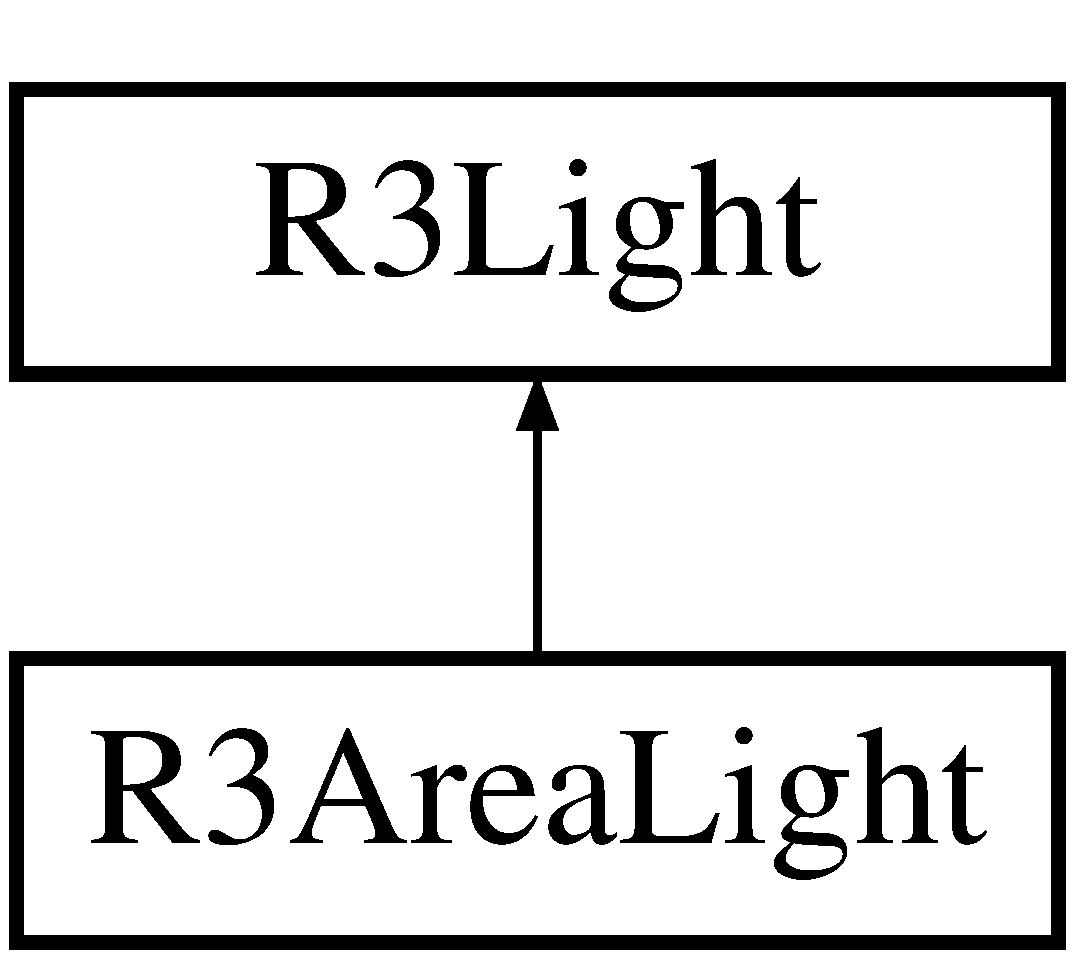
\includegraphics[height=2.000000cm]{class_r3_area_light}
\end{center}
\end{figure}
\subsection*{Public Member Functions}
\begin{DoxyCompactItemize}
\item 
{\bfseries R3\+Area\+Light} (const \hyperlink{class_r3_area_light}{R3\+Area\+Light} \&light)\hypertarget{class_r3_area_light_a748ae029d0eb462820fdd63257b830b7}{}\label{class_r3_area_light_a748ae029d0eb462820fdd63257b830b7}

\item 
{\bfseries R3\+Area\+Light} (const \hyperlink{class_r3_point}{R3\+Point} \&position, R\+N\+Length radius, const \hyperlink{class_r3_vector}{R3\+Vector} \&direction, const \hyperlink{class_r_n_rgb}{R\+N\+Rgb} \&color, R\+N\+Scalar intensity=1.\+0, R\+N\+Boolean active=T\+R\+UE, R\+N\+Scalar ca=0, R\+N\+Scalar la=0, R\+N\+Scalar qa=1)\hypertarget{class_r3_area_light_ac64c5e446b288f20e3ce2eb2ac0a9d6e}{}\label{class_r3_area_light_ac64c5e446b288f20e3ce2eb2ac0a9d6e}

\item 
const \hyperlink{class_r3_point}{R3\+Point} \& {\bfseries Position} (void) const \hypertarget{class_r3_area_light_a58d4f0e59df154b23caf9865b1964963}{}\label{class_r3_area_light_a58d4f0e59df154b23caf9865b1964963}

\item 
const \hyperlink{class_r3_vector}{R3\+Vector} \& {\bfseries Direction} (void) const \hypertarget{class_r3_area_light_a2237d8ce9d68a0e29aeaf0c721fe044c}{}\label{class_r3_area_light_a2237d8ce9d68a0e29aeaf0c721fe044c}

\item 
const R\+N\+Length {\bfseries Radius} (void) const \hypertarget{class_r3_area_light_abc72b49ada3ba83f8ac3cb6518590cb8}{}\label{class_r3_area_light_abc72b49ada3ba83f8ac3cb6518590cb8}

\item 
const R\+N\+Scalar {\bfseries Constant\+Attenuation} (void) const \hypertarget{class_r3_area_light_a3739d70c266fa59b9d9fb74ae608d2b2}{}\label{class_r3_area_light_a3739d70c266fa59b9d9fb74ae608d2b2}

\item 
const R\+N\+Scalar {\bfseries Linear\+Attenuation} (void) const \hypertarget{class_r3_area_light_a38debca62d6662908357532459f3e6f5}{}\label{class_r3_area_light_a38debca62d6662908357532459f3e6f5}

\item 
const R\+N\+Scalar {\bfseries Quadratic\+Attenuation} (void) const \hypertarget{class_r3_area_light_ab16c817199b30019b33570d86837fb4f}{}\label{class_r3_area_light_ab16c817199b30019b33570d86837fb4f}

\item 
virtual void {\bfseries Set\+Position} (const \hyperlink{class_r3_point}{R3\+Point} \&position)\hypertarget{class_r3_area_light_a0e775ccfabb5ea341178e52ee1a7ef22}{}\label{class_r3_area_light_a0e775ccfabb5ea341178e52ee1a7ef22}

\item 
virtual void {\bfseries Set\+Direction} (const \hyperlink{class_r3_vector}{R3\+Vector} \&direction)\hypertarget{class_r3_area_light_ad2cee2e31fb6540d305703c4cd5b4a8e}{}\label{class_r3_area_light_ad2cee2e31fb6540d305703c4cd5b4a8e}

\item 
virtual void {\bfseries Set\+Radius} (R\+N\+Length radius)\hypertarget{class_r3_area_light_a8583ca7b46e03d2a2aea02f68b32792d}{}\label{class_r3_area_light_a8583ca7b46e03d2a2aea02f68b32792d}

\item 
virtual void {\bfseries Set\+Constant\+Attenuation} (R\+N\+Scalar ca)\hypertarget{class_r3_area_light_ad3b981a935238c12978394b3aef9feaa}{}\label{class_r3_area_light_ad3b981a935238c12978394b3aef9feaa}

\item 
virtual void {\bfseries Set\+Linear\+Attenuation} (R\+N\+Scalar la)\hypertarget{class_r3_area_light_a0e2b9c9e544af15c84484cd4297d5332}{}\label{class_r3_area_light_a0e2b9c9e544af15c84484cd4297d5332}

\item 
virtual void {\bfseries Set\+Quadratic\+Attenuation} (R\+N\+Scalar qa)\hypertarget{class_r3_area_light_a7268288d6ec3bb0d8db71205f8056614}{}\label{class_r3_area_light_a7268288d6ec3bb0d8db71205f8056614}

\item 
virtual \hyperlink{class_r_n_rgb}{R\+N\+Rgb} {\bfseries Reflection} (const \hyperlink{class_r3_brdf}{R3\+Brdf} \&brdf, const \hyperlink{class_r3_point}{R3\+Point} \&eye, const \hyperlink{class_r3_point}{R3\+Point} \&point, const \hyperlink{class_r3_vector}{R3\+Vector} \&normal) const \hypertarget{class_r3_area_light_a74eceeff72e14df474b8dc1728b09c44}{}\label{class_r3_area_light_a74eceeff72e14df474b8dc1728b09c44}

\item 
virtual \hyperlink{class_r_n_rgb}{R\+N\+Rgb} {\bfseries Diffuse\+Reflection} (const \hyperlink{class_r3_brdf}{R3\+Brdf} \&brdf, const \hyperlink{class_r3_point}{R3\+Point} \&point, const \hyperlink{class_r3_vector}{R3\+Vector} \&normal) const \hypertarget{class_r3_area_light_ab4fe8cd7d89692bd7d03f2b0e910aaa5}{}\label{class_r3_area_light_ab4fe8cd7d89692bd7d03f2b0e910aaa5}

\item 
virtual \hyperlink{class_r_n_rgb}{R\+N\+Rgb} {\bfseries Specular\+Reflection} (const \hyperlink{class_r3_brdf}{R3\+Brdf} \&brdf, const \hyperlink{class_r3_point}{R3\+Point} \&eye, const \hyperlink{class_r3_point}{R3\+Point} \&point, const \hyperlink{class_r3_vector}{R3\+Vector} \&normal) const \hypertarget{class_r3_area_light_a506eae3d2a4270b1b25f5b92578b5636}{}\label{class_r3_area_light_a506eae3d2a4270b1b25f5b92578b5636}

\item 
virtual void {\bfseries Draw} (int i) const \hypertarget{class_r3_area_light_ab900beffb664cfa6b3b4ae300b0389b5}{}\label{class_r3_area_light_ab900beffb664cfa6b3b4ae300b0389b5}

\item 
{\bfseries R\+N\+\_\+\+C\+L\+A\+S\+S\+\_\+\+T\+Y\+P\+E\+\_\+\+D\+E\+C\+L\+A\+R\+A\+T\+I\+O\+NS} (\hyperlink{class_r3_area_light}{R3\+Area\+Light})\hypertarget{class_r3_area_light_a8cb9498bd5bf548faf072b213f7addbe}{}\label{class_r3_area_light_a8cb9498bd5bf548faf072b213f7addbe}

\end{DoxyCompactItemize}


The documentation for this class was generated from the following files\+:\begin{DoxyCompactItemize}
\item 
R3\+Graphics/R3\+Area\+Light.\+h\item 
R3\+Graphics/R3\+Area\+Light.\+cpp\end{DoxyCompactItemize}

\hypertarget{class_r3_base}{}\section{R3\+Base Class Reference}
\label{class_r3_base}\index{R3\+Base@{R3\+Base}}


The documentation for this class was generated from the following file\+:\begin{DoxyCompactItemize}
\item 
R3\+Shapes/R3\+Base.\+h\end{DoxyCompactItemize}

\hypertarget{class_r3_box}{}\section{R3\+Box Class Reference}
\label{class_r3_box}\index{R3\+Box@{R3\+Box}}
Inheritance diagram for R3\+Box\+:\begin{figure}[H]
\begin{center}
\leavevmode
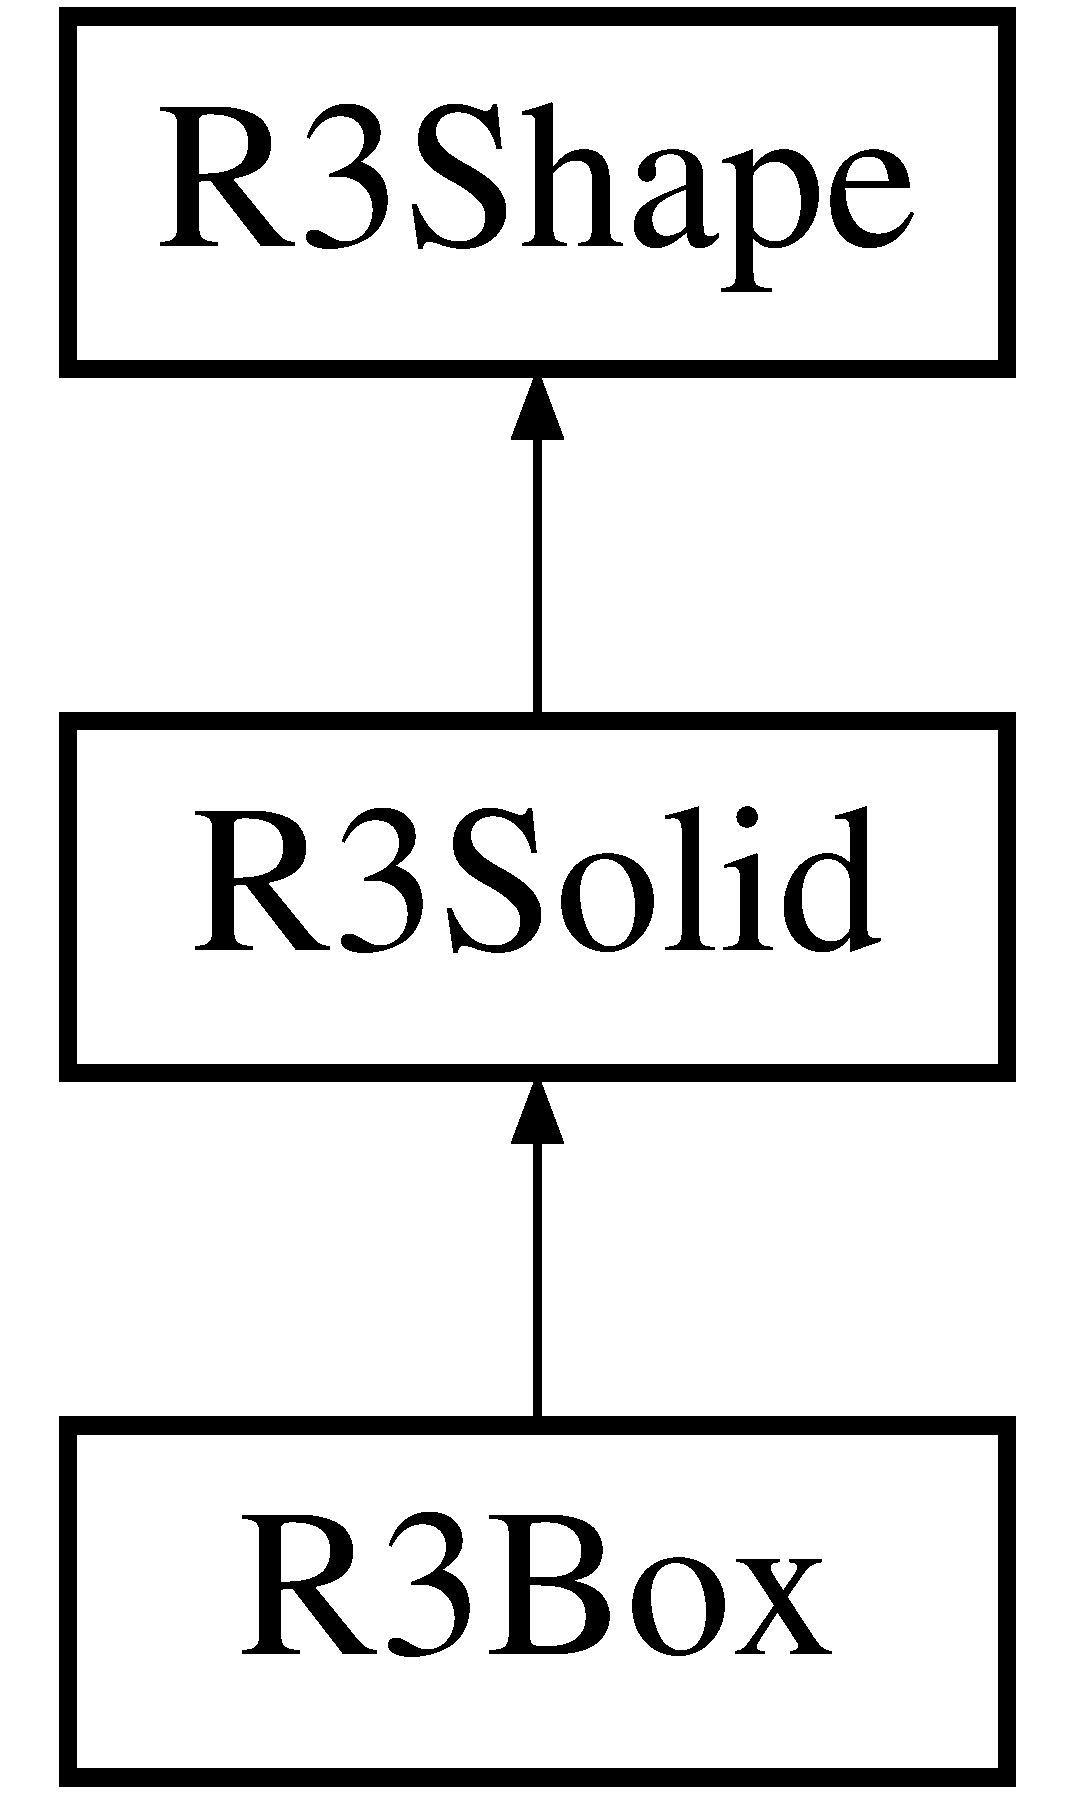
\includegraphics[height=3.000000cm]{class_r3_box}
\end{center}
\end{figure}
\subsection*{Public Member Functions}
\begin{DoxyCompactItemize}
\item 
{\bfseries R3\+Box} (const \hyperlink{class_r3_box}{R3\+Box} \&\hyperlink{structbox}{box})\hypertarget{class_r3_box_a612a8e476d95818c33face7502e2decf}{}\label{class_r3_box_a612a8e476d95818c33face7502e2decf}

\item 
{\bfseries R3\+Box} (const \hyperlink{class_r3_point}{R3\+Point} \&min, const \hyperlink{class_r3_point}{R3\+Point} \&max)\hypertarget{class_r3_box_acf6fa8a44ef5e89d6d3c036ed30b8cf8}{}\label{class_r3_box_acf6fa8a44ef5e89d6d3c036ed30b8cf8}

\item 
{\bfseries R3\+Box} (R\+N\+Coord xmin, R\+N\+Coord ymin, R\+N\+Coord zmin, R\+N\+Coord xmax, R\+N\+Coord ymax, R\+N\+Coord zmax)\hypertarget{class_r3_box_a0f8f2d3ad4745058c22764cedbd8cf47}{}\label{class_r3_box_a0f8f2d3ad4745058c22764cedbd8cf47}

\item 
const R\+N\+Coord {\bfseries X\+Min} (void) const \hypertarget{class_r3_box_ab0bfdca027902805aab8ef82dfaaf241}{}\label{class_r3_box_ab0bfdca027902805aab8ef82dfaaf241}

\item 
const R\+N\+Coord {\bfseries Y\+Min} (void) const \hypertarget{class_r3_box_ac104b65e94ac2099556fe4336da197a2}{}\label{class_r3_box_ac104b65e94ac2099556fe4336da197a2}

\item 
const R\+N\+Coord {\bfseries Z\+Min} (void) const \hypertarget{class_r3_box_afbc351c2f36e60cc7f43d674bab10fb0}{}\label{class_r3_box_afbc351c2f36e60cc7f43d674bab10fb0}

\item 
const R\+N\+Coord {\bfseries X\+Max} (void) const \hypertarget{class_r3_box_a01963da986d89fbbf6bab0239c7a6d13}{}\label{class_r3_box_a01963da986d89fbbf6bab0239c7a6d13}

\item 
const R\+N\+Coord {\bfseries Y\+Max} (void) const \hypertarget{class_r3_box_a663e215b8d254c29271c1e910aaae4cc}{}\label{class_r3_box_a663e215b8d254c29271c1e910aaae4cc}

\item 
const R\+N\+Coord {\bfseries Z\+Max} (void) const \hypertarget{class_r3_box_a15c550c15997bbacdd9f91b27125600e}{}\label{class_r3_box_a15c550c15997bbacdd9f91b27125600e}

\item 
const R\+N\+Coord {\bfseries Coord} (R\+N\+Direction dir, R\+N\+Dimension dim) const \hypertarget{class_r3_box_a1770ca5eeb37cd3cdef00a44fa8217f7}{}\label{class_r3_box_a1770ca5eeb37cd3cdef00a44fa8217f7}

\item 
const \hyperlink{class_r3_point}{R3\+Point} \& {\bfseries Min} (void) const \hypertarget{class_r3_box_a0141f7a79d1d174436e02a78663de034}{}\label{class_r3_box_a0141f7a79d1d174436e02a78663de034}

\item 
const \hyperlink{class_r3_point}{R3\+Point} \& {\bfseries Max} (void) const \hypertarget{class_r3_box_a3cc49c8bd2bb7ab30efa7bf6d772f26f}{}\label{class_r3_box_a3cc49c8bd2bb7ab30efa7bf6d772f26f}

\item 
const \hyperlink{class_r3_point}{R3\+Point} {\bfseries Corner} (R\+N\+Octant octant) const \hypertarget{class_r3_box_aa6b5fbef1fcef288689d778abf7352f0}{}\label{class_r3_box_aa6b5fbef1fcef288689d778abf7352f0}

\item 
const \hyperlink{class_r3_point}{R3\+Point} {\bfseries Corner} (R\+N\+Direction xdir, R\+N\+Direction ydir, R\+N\+Direction zdir) const \hypertarget{class_r3_box_adf929e2e9a2140369311a1e4c8fec61b}{}\label{class_r3_box_adf929e2e9a2140369311a1e4c8fec61b}

\item 
const \hyperlink{class_r3_plane}{R3\+Plane} {\bfseries Plane} (R\+N\+Side side) const \hypertarget{class_r3_box_a73ad684a88a4866a29dec4c6ba75a7e1}{}\label{class_r3_box_a73ad684a88a4866a29dec4c6ba75a7e1}

\item 
const \hyperlink{class_r3_plane}{R3\+Plane} {\bfseries Plane} (R\+N\+Direction dir, R\+N\+Dimension dim) const \hypertarget{class_r3_box_a51aa155a1c4d8d64a5b5f77e287d5097}{}\label{class_r3_box_a51aa155a1c4d8d64a5b5f77e287d5097}

\item 
const \hyperlink{class_r3_box}{R3\+Box} {\bfseries Side} (R\+N\+Side side) const \hypertarget{class_r3_box_a439929c5e65d8b4d39b0f2cdc0b699f3}{}\label{class_r3_box_a439929c5e65d8b4d39b0f2cdc0b699f3}

\item 
const \hyperlink{class_r3_box}{R3\+Box} {\bfseries Side} (R\+N\+Direction dir, R\+N\+Dimension dim) const \hypertarget{class_r3_box_a387587128d4af3793753e03fb097e4b8}{}\label{class_r3_box_a387587128d4af3793753e03fb097e4b8}

\item 
const \hyperlink{class_r3_box}{R3\+Box} {\bfseries Octant} (R\+N\+Octant octant) const \hypertarget{class_r3_box_a1cb9a067d49c7e7d1987998fcbedc522}{}\label{class_r3_box_a1cb9a067d49c7e7d1987998fcbedc522}

\item 
const \hyperlink{class_r3_box}{R3\+Box} {\bfseries Octant} (R\+N\+Direction xdir, R\+N\+Direction ydir, R\+N\+Direction zdir) const \hypertarget{class_r3_box_abb3cbfee2595a696b181c76a41db72c1}{}\label{class_r3_box_abb3cbfee2595a696b181c76a41db72c1}

\item 
const R\+N\+Boolean {\bfseries Is\+Empty} (void) const \hypertarget{class_r3_box_ac9551bfaa5d415874142d943ccc06d6f}{}\label{class_r3_box_ac9551bfaa5d415874142d943ccc06d6f}

\item 
const R\+N\+Boolean {\bfseries Is\+Finite} (void) const \hypertarget{class_r3_box_ab36d3ff954a79140c13e160a70217977}{}\label{class_r3_box_ab36d3ff954a79140c13e160a70217977}

\item 
const int {\bfseries N\+Dimensions} (void) const \hypertarget{class_r3_box_a157e73955ce5ff4ed308869ad6ecc8f5}{}\label{class_r3_box_a157e73955ce5ff4ed308869ad6ecc8f5}

\item 
const int {\bfseries N\+Dimensions\+Along\+Side} (R\+N\+Direction dir, R\+N\+Dimension dim) const \hypertarget{class_r3_box_a1f56820fa3d5964423c0893f471ffd24}{}\label{class_r3_box_a1f56820fa3d5964423c0893f471ffd24}

\item 
const R\+N\+Boolean {\bfseries Is\+Side\+Null} (R\+N\+Direction dir, R\+N\+Dimension dim) const \hypertarget{class_r3_box_a4a441f149ae53efab567abf09242325a}{}\label{class_r3_box_a4a441f149ae53efab567abf09242325a}

\item 
const R\+N\+Boolean {\bfseries Is\+Side\+Linear} (R\+N\+Direction dir, R\+N\+Dimension dim) const \hypertarget{class_r3_box_ab108d7e9baae82fbaad1f2af6b8139f7}{}\label{class_r3_box_ab108d7e9baae82fbaad1f2af6b8139f7}

\item 
const int {\bfseries N\+Dimensions\+Along\+Axis} (const R\+N\+Axis axis) const \hypertarget{class_r3_box_a7acfab0b8840942023c1eafa0315e864}{}\label{class_r3_box_a7acfab0b8840942023c1eafa0315e864}

\item 
const R\+N\+Boolean {\bfseries Is\+Axis\+Null} (const R\+N\+Axis axis) const \hypertarget{class_r3_box_ae07f8f7baa6e3d31446dd8f37b0d2f41}{}\label{class_r3_box_ae07f8f7baa6e3d31446dd8f37b0d2f41}

\item 
const R\+N\+Length {\bfseries X\+Length} (void) const \hypertarget{class_r3_box_a77662ecb0cd9472cf80aa080ee6abf81}{}\label{class_r3_box_a77662ecb0cd9472cf80aa080ee6abf81}

\item 
const R\+N\+Length {\bfseries Y\+Length} (void) const \hypertarget{class_r3_box_a7948b759ff9108cd8683fdb6beb319fc}{}\label{class_r3_box_a7948b759ff9108cd8683fdb6beb319fc}

\item 
const R\+N\+Length {\bfseries Z\+Length} (void) const \hypertarget{class_r3_box_ab206274e5e0a8a6fa8547c885e643798}{}\label{class_r3_box_ab206274e5e0a8a6fa8547c885e643798}

\item 
const R\+N\+Length {\bfseries Axis\+Length} (const R\+N\+Axis axis) const \hypertarget{class_r3_box_ad8543f4627a228193455fd4d42b3834d}{}\label{class_r3_box_ad8543f4627a228193455fd4d42b3834d}

\item 
const R\+N\+Length {\bfseries Diagonal\+Length} (void) const \hypertarget{class_r3_box_aadd3d7d4162ab84c5b7065ca0b713a16}{}\label{class_r3_box_aadd3d7d4162ab84c5b7065ca0b713a16}

\item 
const R\+N\+Length {\bfseries X\+Radius} (void) const \hypertarget{class_r3_box_ac5ca62a8f40ea3ad44feeacf06cc9b73}{}\label{class_r3_box_ac5ca62a8f40ea3ad44feeacf06cc9b73}

\item 
const R\+N\+Length {\bfseries Y\+Radius} (void) const \hypertarget{class_r3_box_ac8551f4dfc7ffd09fc27ed479a10c05d}{}\label{class_r3_box_ac8551f4dfc7ffd09fc27ed479a10c05d}

\item 
const R\+N\+Length {\bfseries Z\+Radius} (void) const \hypertarget{class_r3_box_aaedb25811c736eeca6efdada04d09df5}{}\label{class_r3_box_aaedb25811c736eeca6efdada04d09df5}

\item 
const R\+N\+Length {\bfseries Axis\+Radius} (const R\+N\+Axis axis) const \hypertarget{class_r3_box_a090d3b76304705244653f687d6ea4a02}{}\label{class_r3_box_a090d3b76304705244653f687d6ea4a02}

\item 
const R\+N\+Length {\bfseries Diagonal\+Radius} (void) const \hypertarget{class_r3_box_ae9154548f38c76780b9eb078201ea107}{}\label{class_r3_box_ae9154548f38c76780b9eb078201ea107}

\item 
const R\+N\+Coord {\bfseries X\+Center} (void) const \hypertarget{class_r3_box_aec47255955e21b9d0febee73d208761b}{}\label{class_r3_box_aec47255955e21b9d0febee73d208761b}

\item 
const R\+N\+Coord {\bfseries Y\+Center} (void) const \hypertarget{class_r3_box_addaefb57510388295c1b4c4b984cab7a}{}\label{class_r3_box_addaefb57510388295c1b4c4b984cab7a}

\item 
const R\+N\+Coord {\bfseries Z\+Center} (void) const \hypertarget{class_r3_box_a4590f4961f289f37e4754861f66022c5}{}\label{class_r3_box_a4590f4961f289f37e4754861f66022c5}

\item 
const R\+N\+Coord {\bfseries Axis\+Center} (const R\+N\+Axis axis) const \hypertarget{class_r3_box_ac6eee5334ede0ffbb56bd1f042f6966f}{}\label{class_r3_box_ac6eee5334ede0ffbb56bd1f042f6966f}

\item 
const R\+N\+Axis {\bfseries Shortest\+Axis} (void) const \hypertarget{class_r3_box_a88621b7ede139db1109a7bc2bbe09781}{}\label{class_r3_box_a88621b7ede139db1109a7bc2bbe09781}

\item 
const R\+N\+Axis {\bfseries Longest\+Axis} (void) const \hypertarget{class_r3_box_a4db8775ddcc344d14efe36133f3f7ea3}{}\label{class_r3_box_a4db8775ddcc344d14efe36133f3f7ea3}

\item 
const R\+N\+Length {\bfseries Shortest\+Axis\+Length} (void) const \hypertarget{class_r3_box_a97ec98c6727a32305819f79dfda94a9b}{}\label{class_r3_box_a97ec98c6727a32305819f79dfda94a9b}

\item 
const R\+N\+Length {\bfseries Longest\+Axis\+Length} (void) const \hypertarget{class_r3_box_a36109342fc988d494faa8efa56d5b923}{}\label{class_r3_box_a36109342fc988d494faa8efa56d5b923}

\item 
virtual const R\+N\+Boolean {\bfseries Is\+Point} (void) const \hypertarget{class_r3_box_a35efa8055aa0aea477dbbe98c9104ec1}{}\label{class_r3_box_a35efa8055aa0aea477dbbe98c9104ec1}

\item 
virtual const R\+N\+Boolean {\bfseries Is\+Linear} (void) const \hypertarget{class_r3_box_ab4e87edc7b5613e8464f60f0eca085a2}{}\label{class_r3_box_ab4e87edc7b5613e8464f60f0eca085a2}

\item 
virtual const R\+N\+Boolean {\bfseries Is\+Planar} (void) const \hypertarget{class_r3_box_ae362c70e0dd7c11711b690a5b183a2f1}{}\label{class_r3_box_ae362c70e0dd7c11711b690a5b183a2f1}

\item 
virtual const R\+N\+Boolean {\bfseries Is\+Convex} (void) const \hypertarget{class_r3_box_a754c9694b07831b50faed2a003caed2f}{}\label{class_r3_box_a754c9694b07831b50faed2a003caed2f}

\item 
virtual const \hyperlink{class_r_n_interval}{R\+N\+Interval} {\bfseries N\+Facets} (void) const \hypertarget{class_r3_box_ae405e2bd926c5c1b2acd638c2d65db46}{}\label{class_r3_box_ae405e2bd926c5c1b2acd638c2d65db46}

\item 
virtual const R\+N\+Area {\bfseries Area} (void) const \hypertarget{class_r3_box_a3c1a48dfbb4877b936b43e8094a50266}{}\label{class_r3_box_a3c1a48dfbb4877b936b43e8094a50266}

\item 
virtual const R\+N\+Volume {\bfseries Volume} (void) const \hypertarget{class_r3_box_a22730c07ecb4f82db36f78de4bb9e36b}{}\label{class_r3_box_a22730c07ecb4f82db36f78de4bb9e36b}

\item 
virtual const \hyperlink{class_r3_point}{R3\+Point} {\bfseries Centroid} (void) const \hypertarget{class_r3_box_a7bd768acbb097d1e8d931dff8cbc1d0c}{}\label{class_r3_box_a7bd768acbb097d1e8d931dff8cbc1d0c}

\item 
virtual const \hyperlink{class_r3_point}{R3\+Point} {\bfseries Closest\+Point} (const \hyperlink{class_r3_point}{R3\+Point} \&point) const \hypertarget{class_r3_box_a53203cbdf800dfa96a30e9a576e576f3}{}\label{class_r3_box_a53203cbdf800dfa96a30e9a576e576f3}

\item 
virtual const \hyperlink{class_r3_point}{R3\+Point} {\bfseries Furthest\+Point} (const \hyperlink{class_r3_point}{R3\+Point} \&point) const \hypertarget{class_r3_box_ac67bc6b8e570d794de61ffc77aec190e}{}\label{class_r3_box_ac67bc6b8e570d794de61ffc77aec190e}

\item 
virtual const \hyperlink{class_r3_shape}{R3\+Shape} \& {\bfseries B\+Shape} (void) const \hypertarget{class_r3_box_adec5d24b08a8b0dd7e5ba34588229d4f}{}\label{class_r3_box_adec5d24b08a8b0dd7e5ba34588229d4f}

\item 
virtual const \hyperlink{class_r3_box}{R3\+Box} {\bfseries B\+Box} (void) const \hypertarget{class_r3_box_a2d2bfc9e353c46e8ed2f1136fe9f12bd}{}\label{class_r3_box_a2d2bfc9e353c46e8ed2f1136fe9f12bd}

\item 
virtual const \hyperlink{class_r3_sphere}{R3\+Sphere} {\bfseries B\+Sphere} (void) const \hypertarget{class_r3_box_a190a501b96242d332a209aa79b211597}{}\label{class_r3_box_a190a501b96242d332a209aa79b211597}

\item 
virtual void {\bfseries Empty} (void)\hypertarget{class_r3_box_a92f9ae0fc669607c231840916dd369c5}{}\label{class_r3_box_a92f9ae0fc669607c231840916dd369c5}

\item 
virtual void {\bfseries Inflate} (R\+N\+Scalar fraction)\hypertarget{class_r3_box_a20f82081a2b473f0a7fe5275fe62a584}{}\label{class_r3_box_a20f82081a2b473f0a7fe5275fe62a584}

\item 
virtual void {\bfseries Translate} (const \hyperlink{class_r3_vector}{R3\+Vector} \&vector)\hypertarget{class_r3_box_a8acc8b24871c7f3c8a75a6345af9c755}{}\label{class_r3_box_a8acc8b24871c7f3c8a75a6345af9c755}

\item 
virtual void {\bfseries Union} (const \hyperlink{class_r3_point}{R3\+Point} \&point)\hypertarget{class_r3_box_a4a1eb61e7c9d419b88efc281bfdee3f2}{}\label{class_r3_box_a4a1eb61e7c9d419b88efc281bfdee3f2}

\item 
virtual void {\bfseries Union} (const \hyperlink{class_r3_box}{R3\+Box} \&\hyperlink{structbox}{box})\hypertarget{class_r3_box_a201f7f10005cc7ad64ef563e89312d62}{}\label{class_r3_box_a201f7f10005cc7ad64ef563e89312d62}

\item 
virtual void {\bfseries Union} (const \hyperlink{class_r3_sphere}{R3\+Sphere} \&sphere)\hypertarget{class_r3_box_ad814755efca4476f59ee055b571e614e}{}\label{class_r3_box_ad814755efca4476f59ee055b571e614e}

\item 
virtual void {\bfseries Intersect} (const \hyperlink{class_r3_box}{R3\+Box} \&\hyperlink{structbox}{box})\hypertarget{class_r3_box_ab18b9f4364083a0143ae99c43babc7d8}{}\label{class_r3_box_ab18b9f4364083a0143ae99c43babc7d8}

\item 
virtual void {\bfseries Transform} (const \hyperlink{class_r3_transformation}{R3\+Transformation} \&transformation)\hypertarget{class_r3_box_aa9255cbbc9c7cc9244a17f5dc79058fe}{}\label{class_r3_box_aa9255cbbc9c7cc9244a17f5dc79058fe}

\item 
virtual void {\bfseries Reset} (const \hyperlink{class_r3_point}{R3\+Point} \&min, const \hyperlink{class_r3_point}{R3\+Point} \&max)\hypertarget{class_r3_box_aae9033153563426386648cc48d064879}{}\label{class_r3_box_aae9033153563426386648cc48d064879}

\item 
virtual void {\bfseries Draw} (const \hyperlink{class_r_n_flags}{R3\+Draw\+Flags} draw\+\_\+flags=R3\+\_\+\+D\+E\+F\+A\+U\+L\+T\+\_\+\+D\+R\+A\+W\+\_\+\+F\+L\+A\+GS) const \hypertarget{class_r3_box_aa4b54970958dfc3d09283985ba0d30c9}{}\label{class_r3_box_aa4b54970958dfc3d09283985ba0d30c9}

\item 
R\+N\+Boolean {\bfseries operator==} (const \hyperlink{class_r3_box}{R3\+Box} \&\hyperlink{structbox}{box}) const \hypertarget{class_r3_box_a1b667d365e402dd1b4449e93dd906237}{}\label{class_r3_box_a1b667d365e402dd1b4449e93dd906237}

\item 
R\+N\+Boolean {\bfseries operator!=} (const \hyperlink{class_r3_box}{R3\+Box} \&\hyperlink{structbox}{box}) const \hypertarget{class_r3_box_ac87e3d69359ea2e7cdc698b548f71347}{}\label{class_r3_box_ac87e3d69359ea2e7cdc698b548f71347}

\item 
{\bfseries R\+N\+\_\+\+C\+L\+A\+S\+S\+\_\+\+T\+Y\+P\+E\+\_\+\+D\+E\+C\+L\+A\+R\+A\+T\+I\+O\+NS} (\hyperlink{class_r3_box}{R3\+Box})\hypertarget{class_r3_box_a2b228f65063fefe5058696f3b254688f}{}\label{class_r3_box_a2b228f65063fefe5058696f3b254688f}

\item 
{\bfseries R3\+\_\+\+S\+H\+A\+P\+E\+\_\+\+R\+E\+L\+A\+T\+I\+O\+N\+S\+H\+I\+P\+\_\+\+D\+E\+C\+L\+A\+R\+A\+T\+I\+O\+NS} (\hyperlink{class_r3_box}{R3\+Box})\hypertarget{class_r3_box_a36d44c02426cba12ed2b124acca5bc36}{}\label{class_r3_box_a36d44c02426cba12ed2b124acca5bc36}

\item 
const \hyperlink{class_r3_point}{R3\+Point} \& {\bfseries operator\mbox{[}$\,$\mbox{]}} (R\+N\+Direction dir) const \hypertarget{class_r3_box_a0218b145a9df7010e14808794f5e952b}{}\label{class_r3_box_a0218b145a9df7010e14808794f5e952b}

\item 
\hyperlink{class_r3_point}{R3\+Point} \& {\bfseries operator\mbox{[}$\,$\mbox{]}} (R\+N\+Direction dir)\hypertarget{class_r3_box_a7db3d21fa3b3189ad759cf49e2f7d157}{}\label{class_r3_box_a7db3d21fa3b3189ad759cf49e2f7d157}

\end{DoxyCompactItemize}


The documentation for this class was generated from the following files\+:\begin{DoxyCompactItemize}
\item 
R3\+Shapes/R3\+Box.\+h\item 
R3\+Shapes/R3\+Box.\+cpp\item 
R3\+Shapes/R3\+Draw.\+cpp\end{DoxyCompactItemize}

\hypertarget{class_r3_brdf}{}\section{R3\+Brdf Class Reference}
\label{class_r3_brdf}\index{R3\+Brdf@{R3\+Brdf}}
\subsection*{Public Member Functions}
\begin{DoxyCompactItemize}
\item 
{\bfseries R3\+Brdf} (const \hyperlink{class_r3_brdf}{R3\+Brdf} \&brdf)\hypertarget{class_r3_brdf_af9356f7865445df7289cb70df49fc224}{}\label{class_r3_brdf_af9356f7865445df7289cb70df49fc224}

\item 
{\bfseries R3\+Brdf} (const \hyperlink{class_r_n_rgb}{R\+N\+Rgb} \&rgb, R\+N\+Scalar shininess=0.\+0, R\+N\+Scalar opacity=1.\+0, R\+N\+Scalar indexofrefraction=1.\+0)\hypertarget{class_r3_brdf_a57515b7fc7531baae357780519cc5c3c}{}\label{class_r3_brdf_a57515b7fc7531baae357780519cc5c3c}

\item 
{\bfseries R3\+Brdf} (R\+N\+Scalar red, R\+N\+Scalar green, R\+N\+Scalar blue, R\+N\+Scalar shininess=0.\+0, R\+N\+Scalar opacity=1.\+0, R\+N\+Scalar indexofrefraction=1.\+0)\hypertarget{class_r3_brdf_ab78895e436d411f4182aa2adf018149b}{}\label{class_r3_brdf_ab78895e436d411f4182aa2adf018149b}

\item 
{\bfseries R3\+Brdf} (const \hyperlink{class_r_n_rgb}{R\+N\+Rgb} \&ambient, const \hyperlink{class_r_n_rgb}{R\+N\+Rgb} \&diffuse, const \hyperlink{class_r_n_rgb}{R\+N\+Rgb} \&specular, const \hyperlink{class_r_n_rgb}{R\+N\+Rgb} \&emission, R\+N\+Scalar shininess=0.\+0, R\+N\+Scalar opacity=1.\+0, R\+N\+Scalar indexofrefraction=1.\+0)\hypertarget{class_r3_brdf_a1ef52495ab0ed04d5d477f4bf53fc282}{}\label{class_r3_brdf_a1ef52495ab0ed04d5d477f4bf53fc282}

\item 
{\bfseries R3\+Brdf} (const \hyperlink{class_r_n_rgb}{R\+N\+Rgb} \&ambient, const \hyperlink{class_r_n_rgb}{R\+N\+Rgb} \&diffuse, const \hyperlink{class_r_n_rgb}{R\+N\+Rgb} \&specular, const \hyperlink{class_r_n_rgb}{R\+N\+Rgb} \&transmission, const \hyperlink{class_r_n_rgb}{R\+N\+Rgb} \&emission, R\+N\+Scalar shininess=0.\+0, R\+N\+Scalar indexofrefraction=1.\+0)\hypertarget{class_r3_brdf_a474c183231e8e75b0567b40e6cbe6852}{}\label{class_r3_brdf_a474c183231e8e75b0567b40e6cbe6852}

\item 
const \hyperlink{class_r_n_rgb}{R\+N\+Rgb} \& {\bfseries Ambient} (void) const \hypertarget{class_r3_brdf_a408a8070d6aaafd7e70e070347af70b1}{}\label{class_r3_brdf_a408a8070d6aaafd7e70e070347af70b1}

\item 
const \hyperlink{class_r_n_rgb}{R\+N\+Rgb} \& {\bfseries Diffuse} (void) const \hypertarget{class_r3_brdf_adce784a5e7fddc843bcbc054096b8c4f}{}\label{class_r3_brdf_adce784a5e7fddc843bcbc054096b8c4f}

\item 
const \hyperlink{class_r_n_rgb}{R\+N\+Rgb} \& {\bfseries Specular} (void) const \hypertarget{class_r3_brdf_ad919fa8cdc2f4d9d7a62d87608a569cd}{}\label{class_r3_brdf_ad919fa8cdc2f4d9d7a62d87608a569cd}

\item 
const \hyperlink{class_r_n_rgb}{R\+N\+Rgb} \& {\bfseries Transmission} (void) const \hypertarget{class_r3_brdf_a489b21c16a877e131dcb014eaa83011c}{}\label{class_r3_brdf_a489b21c16a877e131dcb014eaa83011c}

\item 
const \hyperlink{class_r_n_rgb}{R\+N\+Rgb} \& {\bfseries Emission} (void) const \hypertarget{class_r3_brdf_a840588cbc4f2bf9cf990e371db7943e2}{}\label{class_r3_brdf_a840588cbc4f2bf9cf990e371db7943e2}

\item 
const R\+N\+Scalar {\bfseries Shininess} (void) const \hypertarget{class_r3_brdf_aa6b02a3d99da73c2d051fabdc02e59b3}{}\label{class_r3_brdf_aa6b02a3d99da73c2d051fabdc02e59b3}

\item 
const R\+N\+Scalar {\bfseries Opacity} (void) const \hypertarget{class_r3_brdf_a5b7dd03ca9921d16233115aab6a569ca}{}\label{class_r3_brdf_a5b7dd03ca9921d16233115aab6a569ca}

\item 
const R\+N\+Scalar {\bfseries Index\+Of\+Refraction} (void) const \hypertarget{class_r3_brdf_a08ecc6b83f258a1389b3fd5ab5c2c9c3}{}\label{class_r3_brdf_a08ecc6b83f258a1389b3fd5ab5c2c9c3}

\item 
const int {\bfseries Is\+Ambient} (void) const \hypertarget{class_r3_brdf_a645755513d418a8aea142e80a7e26702}{}\label{class_r3_brdf_a645755513d418a8aea142e80a7e26702}

\item 
const int {\bfseries Is\+Diffuse} (void) const \hypertarget{class_r3_brdf_a17d5ec3069b66e9c8f06b937162aa3f2}{}\label{class_r3_brdf_a17d5ec3069b66e9c8f06b937162aa3f2}

\item 
const int {\bfseries Is\+Specular} (void) const \hypertarget{class_r3_brdf_afe58b13d942d0d7b61a7538d44321e2b}{}\label{class_r3_brdf_afe58b13d942d0d7b61a7538d44321e2b}

\item 
const int {\bfseries Is\+Transparent} (void) const \hypertarget{class_r3_brdf_aa40325f67b2353cc792886e48cbbdf97}{}\label{class_r3_brdf_aa40325f67b2353cc792886e48cbbdf97}

\item 
const int {\bfseries Is\+Emissive} (void) const \hypertarget{class_r3_brdf_a9990ddfa6962a8441307f58656c54bb5}{}\label{class_r3_brdf_a9990ddfa6962a8441307f58656c54bb5}

\item 
const int {\bfseries Is\+Shiny} (void) const \hypertarget{class_r3_brdf_ae22e21397896f06042ff5caf280fbfe7}{}\label{class_r3_brdf_ae22e21397896f06042ff5caf280fbfe7}

\item 
const \hyperlink{class_r_n_flags}{R\+N\+Flags} {\bfseries Flags} (void) const \hypertarget{class_r3_brdf_a8cacff926084de6548141ea787b5ae4c}{}\label{class_r3_brdf_a8cacff926084de6548141ea787b5ae4c}

\item 
const int {\bfseries ID} (void) const \hypertarget{class_r3_brdf_a92f445ff7c96aa15946a915024b4f8b8}{}\label{class_r3_brdf_a92f445ff7c96aa15946a915024b4f8b8}

\item 
void {\bfseries Set\+Ambient} (const \hyperlink{class_r_n_rgb}{R\+N\+Rgb} \&rgb)\hypertarget{class_r3_brdf_abd6f043e8ad6dc502f4e704526c997a5}{}\label{class_r3_brdf_abd6f043e8ad6dc502f4e704526c997a5}

\item 
void {\bfseries Set\+Diffuse} (const \hyperlink{class_r_n_rgb}{R\+N\+Rgb} \&rgb)\hypertarget{class_r3_brdf_a85803ca36a81fd52fa07a875b5fe1ba2}{}\label{class_r3_brdf_a85803ca36a81fd52fa07a875b5fe1ba2}

\item 
void {\bfseries Set\+Specular} (const \hyperlink{class_r_n_rgb}{R\+N\+Rgb} \&rgb)\hypertarget{class_r3_brdf_afeef687c49b713d5a2362455a58b8975}{}\label{class_r3_brdf_afeef687c49b713d5a2362455a58b8975}

\item 
void {\bfseries Set\+Transmission} (const \hyperlink{class_r_n_rgb}{R\+N\+Rgb} \&rgb)\hypertarget{class_r3_brdf_a516ba01eb26c02fbc190c4c50851dbe3}{}\label{class_r3_brdf_a516ba01eb26c02fbc190c4c50851dbe3}

\item 
void {\bfseries Set\+Emission} (const \hyperlink{class_r_n_rgb}{R\+N\+Rgb} \&rgb)\hypertarget{class_r3_brdf_ac8ff611cf31bbe3795cd9783ac5fa833}{}\label{class_r3_brdf_ac8ff611cf31bbe3795cd9783ac5fa833}

\item 
void {\bfseries Set\+Shininess} (R\+N\+Scalar shininess)\hypertarget{class_r3_brdf_a8842037800a27d1e58cb72b150e0bda9}{}\label{class_r3_brdf_a8842037800a27d1e58cb72b150e0bda9}

\item 
void {\bfseries Set\+Opacity} (R\+N\+Scalar opacity)\hypertarget{class_r3_brdf_acd714a50ea69a513328567d1618ebe9c}{}\label{class_r3_brdf_acd714a50ea69a513328567d1618ebe9c}

\item 
void {\bfseries Set\+Index\+Of\+Refraction} (R\+N\+Scalar indexofrefraction)\hypertarget{class_r3_brdf_aaeed62c18c0eb91a5a15b9c45d4f4b1c}{}\label{class_r3_brdf_aaeed62c18c0eb91a5a15b9c45d4f4b1c}

\item 
void {\bfseries Load} (void) const \hypertarget{class_r3_brdf_af93330f6469a4c800f42a056a15655f5}{}\label{class_r3_brdf_af93330f6469a4c800f42a056a15655f5}

\item 
void {\bfseries Unload} (void) const \hypertarget{class_r3_brdf_ac2aa39a75a3aacb6f966fc96a977ed21}{}\label{class_r3_brdf_ac2aa39a75a3aacb6f966fc96a977ed21}

\item 
void {\bfseries Draw} (R\+N\+Boolean force=F\+A\+L\+SE) const \hypertarget{class_r3_brdf_a3c495da11bb530dc8c4dae2420c7e888}{}\label{class_r3_brdf_a3c495da11bb530dc8c4dae2420c7e888}

\end{DoxyCompactItemize}
\subsection*{Protected Member Functions}
\begin{DoxyCompactItemize}
\item 
void {\bfseries Update} (void)\hypertarget{class_r3_brdf_a7012a3fbcb6b610dcb6f6ca66e818ffc}{}\label{class_r3_brdf_a7012a3fbcb6b610dcb6f6ca66e818ffc}

\item 
void {\bfseries Update\+Flags} (const \hyperlink{class_r_n_flags}{R\+N\+Flags} flags)\hypertarget{class_r3_brdf_a7aa847654676680c2aa7f4bdffeb0051}{}\label{class_r3_brdf_a7aa847654676680c2aa7f4bdffeb0051}

\end{DoxyCompactItemize}


The documentation for this class was generated from the following files\+:\begin{DoxyCompactItemize}
\item 
R3\+Graphics/R3\+Brdf.\+h\item 
R3\+Graphics/R3\+Brdf.\+cpp\end{DoxyCompactItemize}

\hypertarget{class_r3_camera}{}\section{R3\+Camera Class Reference}
\label{class_r3_camera}\index{R3\+Camera@{R3\+Camera}}
\subsection*{Public Member Functions}
\begin{DoxyCompactItemize}
\item 
{\bfseries R3\+Camera} (const \hyperlink{class_r3_coord_system}{R3\+Coord\+System} \&cs, R\+N\+Angle xfov, R\+N\+Angle yfov, R\+N\+Length neardist, R\+N\+Length fardist)\hypertarget{class_r3_camera_a048a9fa556a75fad946f802abfe94a33}{}\label{class_r3_camera_a048a9fa556a75fad946f802abfe94a33}

\item 
{\bfseries R3\+Camera} (const \hyperlink{class_r3_point}{R3\+Point} \&origin, const \hyperlink{class_r3_triad}{R3\+Triad} \&triad, R\+N\+Angle xfov, R\+N\+Angle yfov, R\+N\+Length neardist, R\+N\+Length fardist)\hypertarget{class_r3_camera_a353a3e5700f2f310bec22535e25a28fd}{}\label{class_r3_camera_a353a3e5700f2f310bec22535e25a28fd}

\item 
{\bfseries R3\+Camera} (const \hyperlink{class_r3_point}{R3\+Point} \&origin, const \hyperlink{class_r3_vector}{R3\+Vector} \&towards, const \hyperlink{class_r3_vector}{R3\+Vector} \&up, R\+N\+Angle xfov, R\+N\+Angle yfov, R\+N\+Length neardist, R\+N\+Length fardist)\hypertarget{class_r3_camera_aeb02ab186aa2b8986279b48fed4b3eca}{}\label{class_r3_camera_aeb02ab186aa2b8986279b48fed4b3eca}

\item 
{\bfseries R3\+Camera} (const \hyperlink{class_r3_point}{R3\+Point} \&origin, R\+N\+Angle pitch, R\+N\+Angle yaw, R\+N\+Angle roll, R\+N\+Angle xfov, R\+N\+Angle yfov, R\+N\+Length neardist, R\+N\+Length fardist)\hypertarget{class_r3_camera_a73208317d4b4efdacc1577134b7e4a63}{}\label{class_r3_camera_a73208317d4b4efdacc1577134b7e4a63}

\item 
const \hyperlink{class_r3_point}{R3\+Point} \& {\bfseries Origin} (void) const \hypertarget{class_r3_camera_a025d8679a2de95b019eb6690b90ac0d2}{}\label{class_r3_camera_a025d8679a2de95b019eb6690b90ac0d2}

\item 
const \hyperlink{class_r3_vector}{R3\+Vector} {\bfseries Towards} (void) const \hypertarget{class_r3_camera_a599d7da0c62dbe7611494d829bb877ff}{}\label{class_r3_camera_a599d7da0c62dbe7611494d829bb877ff}

\item 
const \hyperlink{class_r3_vector}{R3\+Vector} \& {\bfseries Backwards} (void) const \hypertarget{class_r3_camera_aadfc999fd6fc5685e5a5023a50ac2ab5}{}\label{class_r3_camera_aadfc999fd6fc5685e5a5023a50ac2ab5}

\item 
const \hyperlink{class_r3_vector}{R3\+Vector} \& {\bfseries Up} (void) const \hypertarget{class_r3_camera_af1b9da48dd6310e48cba5a02ef47e317}{}\label{class_r3_camera_af1b9da48dd6310e48cba5a02ef47e317}

\item 
const \hyperlink{class_r3_vector}{R3\+Vector} {\bfseries Down} (void) const \hypertarget{class_r3_camera_a2f99f59f13ad0081fa39df030f1c098a}{}\label{class_r3_camera_a2f99f59f13ad0081fa39df030f1c098a}

\item 
const \hyperlink{class_r3_vector}{R3\+Vector} \& {\bfseries Right} (void) const \hypertarget{class_r3_camera_a0e6b37e33997aa66c45a9fc8edbbbd50}{}\label{class_r3_camera_a0e6b37e33997aa66c45a9fc8edbbbd50}

\item 
const \hyperlink{class_r3_vector}{R3\+Vector} {\bfseries Left} (void) const \hypertarget{class_r3_camera_a6039cfc31e6bb9d7812971cb4432f3b9}{}\label{class_r3_camera_a6039cfc31e6bb9d7812971cb4432f3b9}

\item 
const R\+N\+Angle {\bfseries Pitch} (void) const \hypertarget{class_r3_camera_ade325c4ec42f61e3d1a098f82027bd66}{}\label{class_r3_camera_ade325c4ec42f61e3d1a098f82027bd66}

\item 
const R\+N\+Angle {\bfseries Yaw} (void) const \hypertarget{class_r3_camera_ad1d4e1a32c81942d994ccbe2ff9c3ed2}{}\label{class_r3_camera_ad1d4e1a32c81942d994ccbe2ff9c3ed2}

\item 
const R\+N\+Angle {\bfseries Roll} (void) const \hypertarget{class_r3_camera_a6ffd57b1a50e6462345be17d9ccc6e4d}{}\label{class_r3_camera_a6ffd57b1a50e6462345be17d9ccc6e4d}

\item 
const R\+N\+Angle {\bfseries X\+F\+OV} (void) const \hypertarget{class_r3_camera_ae68b0112a7d730483d74cc261f741825}{}\label{class_r3_camera_ae68b0112a7d730483d74cc261f741825}

\item 
const R\+N\+Angle {\bfseries Y\+F\+OV} (void) const \hypertarget{class_r3_camera_aa4dcb60504547e48adf4c0fd315a8285}{}\label{class_r3_camera_aa4dcb60504547e48adf4c0fd315a8285}

\item 
const R\+N\+Length {\bfseries Near} (void) const \hypertarget{class_r3_camera_a38683212a50a5ec930fe8ab5929d4d1d}{}\label{class_r3_camera_a38683212a50a5ec930fe8ab5929d4d1d}

\item 
const R\+N\+Length {\bfseries Far} (void) const \hypertarget{class_r3_camera_a4d29c5d22c2e53e64b1a5e2dfc3f2007}{}\label{class_r3_camera_a4d29c5d22c2e53e64b1a5e2dfc3f2007}

\item 
const \hyperlink{class_r3_triad}{R3\+Triad} \& {\bfseries Triad} (void) const \hypertarget{class_r3_camera_a9e0f64d47aa006350219bcac2c0037f0}{}\label{class_r3_camera_a9e0f64d47aa006350219bcac2c0037f0}

\item 
const \hyperlink{class_r3_coord_system}{R3\+Coord\+System} \& {\bfseries Coord\+System} (void) const \hypertarget{class_r3_camera_a9576100d54078536e5867f31fd6e09d8}{}\label{class_r3_camera_a9576100d54078536e5867f31fd6e09d8}

\item 
const \hyperlink{class_r3_halfspace}{R3\+Halfspace} {\bfseries Halfspace} (R\+N\+Direction dir, R\+N\+Dimension dim) const \hypertarget{class_r3_camera_af482e53495748e51343fd1506eef4ef2}{}\label{class_r3_camera_af482e53495748e51343fd1506eef4ef2}

\item 
const \hyperlink{class_r4_matrix}{R4\+Matrix} {\bfseries Perspective} (void) const \hypertarget{class_r3_camera_a83e04168e3c3b9f771036c36a87acbc4}{}\label{class_r3_camera_a83e04168e3c3b9f771036c36a87acbc4}

\item 
const R\+N\+Boolean {\bfseries operator==} (const \hyperlink{class_r3_camera}{R3\+Camera} \&camera) const \hypertarget{class_r3_camera_ac1b333e66d5a4dddf4b1d342053f6cb3}{}\label{class_r3_camera_ac1b333e66d5a4dddf4b1d342053f6cb3}

\item 
const R\+N\+Boolean {\bfseries operator!=} (const \hyperlink{class_r3_camera}{R3\+Camera} \&camera) const \hypertarget{class_r3_camera_a195f5fa8a5695b95a035ef0ac6d5454c}{}\label{class_r3_camera_a195f5fa8a5695b95a035ef0ac6d5454c}

\item 
void {\bfseries Reset} (const \hyperlink{class_r3_point}{R3\+Point} \&origin, const \hyperlink{class_r3_vector}{R3\+Vector} \&towards, const \hyperlink{class_r3_vector}{R3\+Vector} \&up)\hypertarget{class_r3_camera_a9425169ee03f6e3ca852dc346284c1c9}{}\label{class_r3_camera_a9425169ee03f6e3ca852dc346284c1c9}

\item 
void {\bfseries Reposition} (const \hyperlink{class_r3_point}{R3\+Point} \&origin)\hypertarget{class_r3_camera_a9614931af325a72c0385914ced225f0e}{}\label{class_r3_camera_a9614931af325a72c0385914ced225f0e}

\item 
void {\bfseries Reorient} (const \hyperlink{class_r3_vector}{R3\+Vector} \&towards, const \hyperlink{class_r3_vector}{R3\+Vector} \&up)\hypertarget{class_r3_camera_a4a75633f8e01c81a40a0f5e823a3241a}{}\label{class_r3_camera_a4a75633f8e01c81a40a0f5e823a3241a}

\item 
void {\bfseries Reorient} (R\+N\+Angle pitch, R\+N\+Angle yaw, R\+N\+Angle roll)\hypertarget{class_r3_camera_ab5f8497da9194f3792ab4f7a5ba114a1}{}\label{class_r3_camera_ab5f8497da9194f3792ab4f7a5ba114a1}

\item 
void {\bfseries Mirror} (const \hyperlink{class_r3_plane}{R3\+Plane} \&plane)\hypertarget{class_r3_camera_a96234194e954ce5045cb8d4510de72bd}{}\label{class_r3_camera_a96234194e954ce5045cb8d4510de72bd}

\item 
void {\bfseries Set\+Coord\+System} (const \hyperlink{class_r3_coord_system}{R3\+Coord\+System} \&cs)\hypertarget{class_r3_camera_af1d9a9e5420453c338f74b7982a903ef}{}\label{class_r3_camera_af1d9a9e5420453c338f74b7982a903ef}

\item 
void {\bfseries Set\+Origin} (const \hyperlink{class_r3_point}{R3\+Point} \&origin)\hypertarget{class_r3_camera_ad88451b2318bc8101bd6ec133761439f}{}\label{class_r3_camera_ad88451b2318bc8101bd6ec133761439f}

\item 
void {\bfseries Set\+Towards} (const \hyperlink{class_r3_vector}{R3\+Vector} \&towards)\hypertarget{class_r3_camera_a53312c419ccdc131a019c86773622b06}{}\label{class_r3_camera_a53312c419ccdc131a019c86773622b06}

\item 
void {\bfseries Set\+Backwards} (const \hyperlink{class_r3_vector}{R3\+Vector} \&backwards)\hypertarget{class_r3_camera_aca28b6e5d7463ade06168728adae01bc}{}\label{class_r3_camera_aca28b6e5d7463ade06168728adae01bc}

\item 
void {\bfseries Set\+Up} (const \hyperlink{class_r3_vector}{R3\+Vector} \&up)\hypertarget{class_r3_camera_ab6396e059466f0932b27c2b860559444}{}\label{class_r3_camera_ab6396e059466f0932b27c2b860559444}

\item 
void {\bfseries Set\+Down} (const \hyperlink{class_r3_vector}{R3\+Vector} \&down)\hypertarget{class_r3_camera_a779aca97a6621f2d7c346f4533971c70}{}\label{class_r3_camera_a779aca97a6621f2d7c346f4533971c70}

\item 
void {\bfseries Set\+Right} (const \hyperlink{class_r3_vector}{R3\+Vector} \&right)\hypertarget{class_r3_camera_af503b78f050c6284b124648b99101f61}{}\label{class_r3_camera_af503b78f050c6284b124648b99101f61}

\item 
void {\bfseries Set\+Left} (const \hyperlink{class_r3_vector}{R3\+Vector} \&left)\hypertarget{class_r3_camera_ad6abd43608bb36c9bb2bfd78c1705c63}{}\label{class_r3_camera_ad6abd43608bb36c9bb2bfd78c1705c63}

\item 
void {\bfseries Set\+Pitch} (R\+N\+Angle pitch)\hypertarget{class_r3_camera_ad10cc84643d672049e0bae6c033c03c6}{}\label{class_r3_camera_ad10cc84643d672049e0bae6c033c03c6}

\item 
void {\bfseries Set\+Yaw} (R\+N\+Angle pitch)\hypertarget{class_r3_camera_a50b2d4c41efdd3442133860f90b3b5fe}{}\label{class_r3_camera_a50b2d4c41efdd3442133860f90b3b5fe}

\item 
void {\bfseries Set\+Roll} (R\+N\+Angle pitch)\hypertarget{class_r3_camera_ab5228493697ec4db80d323a2084e96db}{}\label{class_r3_camera_ab5228493697ec4db80d323a2084e96db}

\item 
void {\bfseries Set\+F\+OV} (R\+N\+Angle xfov, R\+N\+Angle yfov)\hypertarget{class_r3_camera_a12d5c18e4558d66e556175b8abd4e864}{}\label{class_r3_camera_a12d5c18e4558d66e556175b8abd4e864}

\item 
void {\bfseries Set\+X\+F\+OV} (R\+N\+Angle xfov)\hypertarget{class_r3_camera_a538ccb3d426eca08e56c8da7a274b405}{}\label{class_r3_camera_a538ccb3d426eca08e56c8da7a274b405}

\item 
void {\bfseries Set\+Y\+F\+OV} (R\+N\+Angle yfov)\hypertarget{class_r3_camera_afeb70ad1f48448154c2330cc625d7387}{}\label{class_r3_camera_afeb70ad1f48448154c2330cc625d7387}

\item 
void {\bfseries Set\+Near} (R\+N\+Length neardist)\hypertarget{class_r3_camera_aba6703e86cab9b6b3b1707ff27995642}{}\label{class_r3_camera_aba6703e86cab9b6b3b1707ff27995642}

\item 
void {\bfseries Set\+Far} (R\+N\+Length fardist)\hypertarget{class_r3_camera_aa58204f9bc03f23c891109301e41ae0c}{}\label{class_r3_camera_aa58204f9bc03f23c891109301e41ae0c}

\item 
void {\bfseries Translate} (const \hyperlink{class_r3_vector}{R3\+Vector} \&translation)\hypertarget{class_r3_camera_acde2f9943694dc08fb18326f2b6b622c}{}\label{class_r3_camera_acde2f9943694dc08fb18326f2b6b622c}

\item 
void {\bfseries Rotate} (const \hyperlink{class_r3_vector}{R3\+Vector} \&axis, R\+N\+Angle dtheta)\hypertarget{class_r3_camera_a996ea9491b1c7994bae28dade020148f}{}\label{class_r3_camera_a996ea9491b1c7994bae28dade020148f}

\item 
void {\bfseries Rotate\+Pitch} (R\+N\+Angle dpitch)\hypertarget{class_r3_camera_ae94fd682bea9d2a27355f56543a4ee45}{}\label{class_r3_camera_ae94fd682bea9d2a27355f56543a4ee45}

\item 
void {\bfseries Rotate\+Yaw} (R\+N\+Angle dyaw)\hypertarget{class_r3_camera_ac3f57cc40f592c2b9485f43cf3c5dda3}{}\label{class_r3_camera_ac3f57cc40f592c2b9485f43cf3c5dda3}

\item 
void {\bfseries Rotate\+Roll} (R\+N\+Angle droll)\hypertarget{class_r3_camera_ab2d53d932ba486aa3ec9dfdb52bd867b}{}\label{class_r3_camera_ab2d53d932ba486aa3ec9dfdb52bd867b}

\item 
void {\bfseries Transform} (const \hyperlink{class_r3_transformation}{R3\+Transformation} \&transformation)\hypertarget{class_r3_camera_a293794de29a71b2866b1cf2e794422f0}{}\label{class_r3_camera_a293794de29a71b2866b1cf2e794422f0}

\item 
void {\bfseries Load} (R\+N\+Boolean select\+\_\+mode=F\+A\+L\+SE) const \hypertarget{class_r3_camera_ab33808c4effe5ec426e1135355783056}{}\label{class_r3_camera_ab33808c4effe5ec426e1135355783056}

\item 
void {\bfseries Draw} (void) const \hypertarget{class_r3_camera_a4019a6e50fc04b986499d01f39f0d711}{}\label{class_r3_camera_a4019a6e50fc04b986499d01f39f0d711}

\item 
void {\bfseries Outline} (void) const \hypertarget{class_r3_camera_aeb6e0451ede15559755bee0913514cbc}{}\label{class_r3_camera_aeb6e0451ede15559755bee0913514cbc}

\end{DoxyCompactItemize}


The documentation for this class was generated from the following files\+:\begin{DoxyCompactItemize}
\item 
R3\+Graphics/R3\+Camera.\+h\item 
R3\+Graphics/R3\+Camera.\+cpp\end{DoxyCompactItemize}

\hypertarget{class_r3_circle}{}\section{R3\+Circle Class Reference}
\label{class_r3_circle}\index{R3\+Circle@{R3\+Circle}}
Inheritance diagram for R3\+Circle\+:\begin{figure}[H]
\begin{center}
\leavevmode
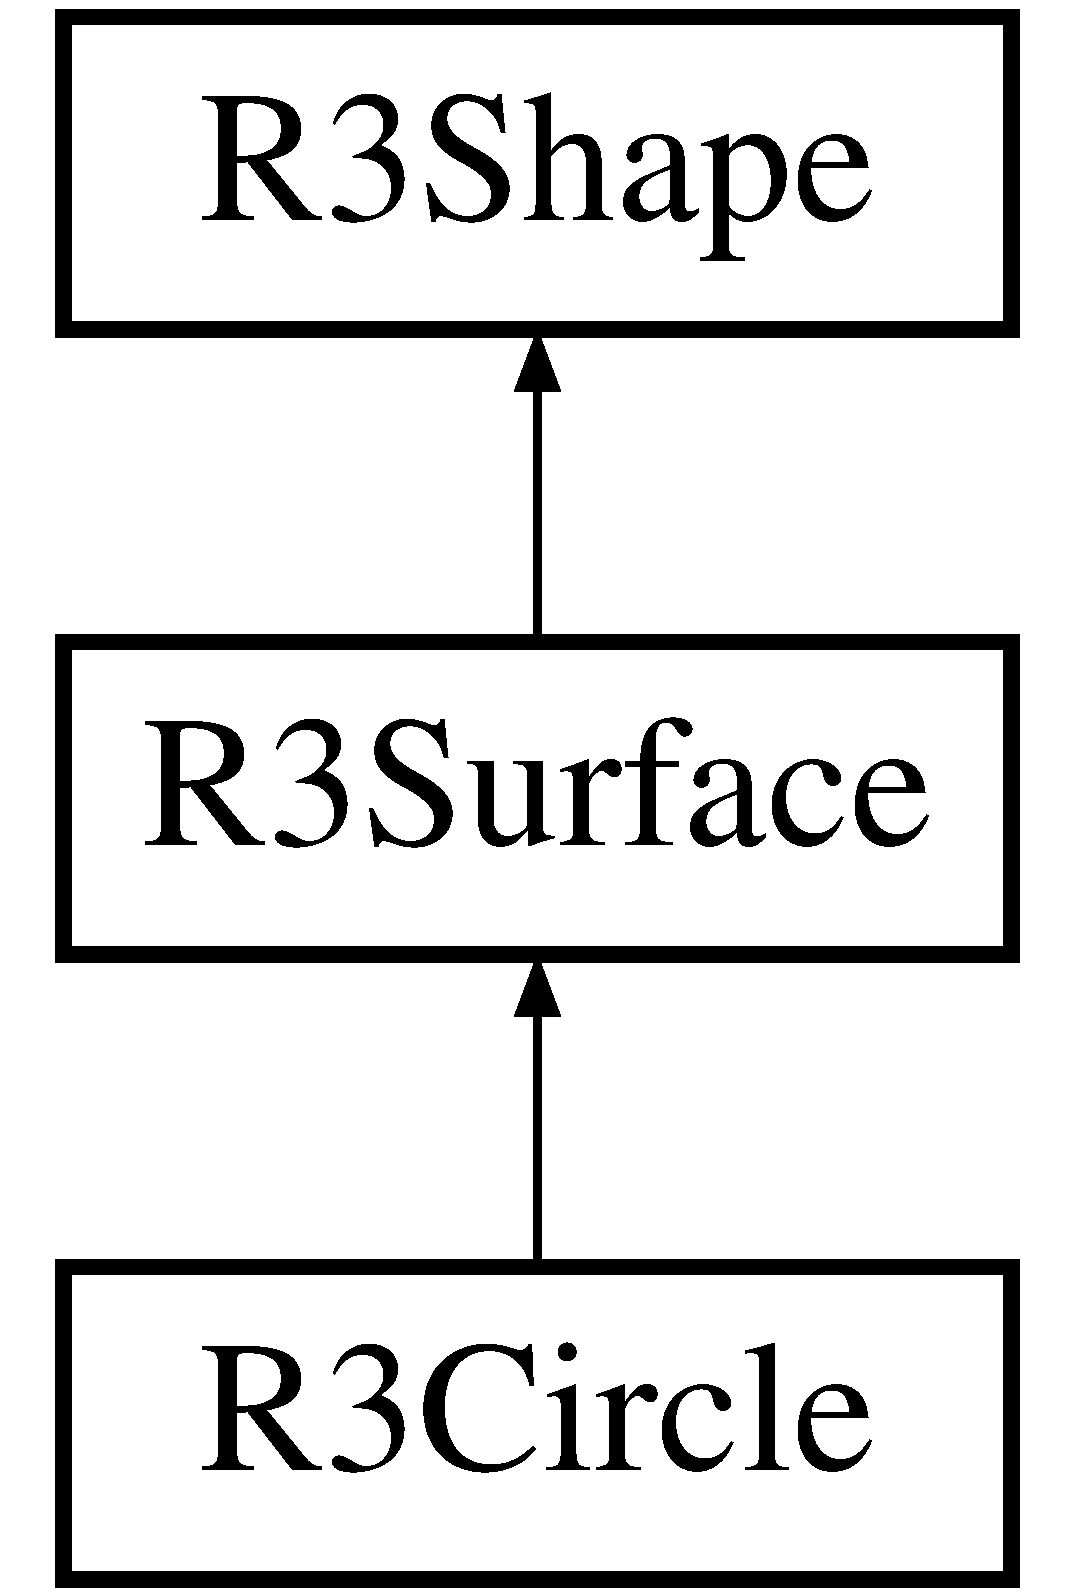
\includegraphics[height=3.000000cm]{class_r3_circle}
\end{center}
\end{figure}
\subsection*{Public Member Functions}
\begin{DoxyCompactItemize}
\item 
{\bfseries R3\+Circle} (const \hyperlink{class_r3_circle}{R3\+Circle} \&circle)\hypertarget{class_r3_circle_abc03b085f6c58c27c2b879c4618e2524}{}\label{class_r3_circle_abc03b085f6c58c27c2b879c4618e2524}

\item 
{\bfseries R3\+Circle} (const \hyperlink{class_r3_point}{R3\+Point} \&center, R\+N\+Length radius, const \hyperlink{class_r3_vector}{R3\+Vector} \&normal)\hypertarget{class_r3_circle_a3d75cc1a0a47e697c5bcec341425cfd0}{}\label{class_r3_circle_a3d75cc1a0a47e697c5bcec341425cfd0}

\item 
{\bfseries R3\+Circle} (const \hyperlink{class_r3_point}{R3\+Point} \&p1, const \hyperlink{class_r3_point}{R3\+Point} \&p2, const \hyperlink{class_r3_point}{R3\+Point} \&p3)\hypertarget{class_r3_circle_ac23f32d620adfb969598854af21d0462}{}\label{class_r3_circle_ac23f32d620adfb969598854af21d0462}

\item 
const \hyperlink{class_r3_point}{R3\+Point} \& {\bfseries Center} (void) const \hypertarget{class_r3_circle_ab9bb28591f1e04767510a809b25c6a2a}{}\label{class_r3_circle_ab9bb28591f1e04767510a809b25c6a2a}

\item 
const R\+N\+Length {\bfseries Radius} (void) const \hypertarget{class_r3_circle_a237dd84ab801203de2c70d0bf6d493d4}{}\label{class_r3_circle_a237dd84ab801203de2c70d0bf6d493d4}

\item 
const \hyperlink{class_r3_plane}{R3\+Plane} \& {\bfseries Plane} (void) const \hypertarget{class_r3_circle_aa041393e95882f07c9a068bd4cbbfd5d}{}\label{class_r3_circle_aa041393e95882f07c9a068bd4cbbfd5d}

\item 
const \hyperlink{class_r3_vector}{R3\+Vector} \& {\bfseries Normal} (void) const \hypertarget{class_r3_circle_aa8621189894c658b13a8eca22b738b48}{}\label{class_r3_circle_aa8621189894c658b13a8eca22b738b48}

\item 
const R\+N\+Boolean {\bfseries Is\+Empty} (void) const \hypertarget{class_r3_circle_ae7e95e27ae82cc6b6fcf97a078bab288}{}\label{class_r3_circle_ae7e95e27ae82cc6b6fcf97a078bab288}

\item 
const R\+N\+Boolean {\bfseries Is\+Finite} (void) const \hypertarget{class_r3_circle_a795fb77b0cbdd7eb3233a375da3ec350}{}\label{class_r3_circle_a795fb77b0cbdd7eb3233a375da3ec350}

\item 
virtual const R\+N\+Boolean {\bfseries Is\+Point} (void) const \hypertarget{class_r3_circle_aff793aae7084bbb76ea3047e5865b0a7}{}\label{class_r3_circle_aff793aae7084bbb76ea3047e5865b0a7}

\item 
virtual const R\+N\+Boolean {\bfseries Is\+Linear} (void) const \hypertarget{class_r3_circle_a76930897ccb495b8e1597356246faf66}{}\label{class_r3_circle_a76930897ccb495b8e1597356246faf66}

\item 
virtual const R\+N\+Boolean {\bfseries Is\+Planar} (void) const \hypertarget{class_r3_circle_af6d955e2c4d1446a7732218c8225869d}{}\label{class_r3_circle_af6d955e2c4d1446a7732218c8225869d}

\item 
virtual const R\+N\+Boolean {\bfseries Is\+Convex} (void) const \hypertarget{class_r3_circle_a3ab653d5336972442246edba6023ad2b}{}\label{class_r3_circle_a3ab653d5336972442246edba6023ad2b}

\item 
virtual const \hyperlink{class_r_n_interval}{R\+N\+Interval} {\bfseries N\+Facets} (void) const \hypertarget{class_r3_circle_a65eff958c61454a5e686679e1d11c78b}{}\label{class_r3_circle_a65eff958c61454a5e686679e1d11c78b}

\item 
virtual const R\+N\+Length {\bfseries Length} (void) const \hypertarget{class_r3_circle_a3d2fa906d2399b2e965829ba2d1cc732}{}\label{class_r3_circle_a3d2fa906d2399b2e965829ba2d1cc732}

\item 
virtual const R\+N\+Area {\bfseries Area} (void) const \hypertarget{class_r3_circle_a0cc7f03fc139d8d8798e1d825a4ed3f2}{}\label{class_r3_circle_a0cc7f03fc139d8d8798e1d825a4ed3f2}

\item 
virtual const \hyperlink{class_r3_point}{R3\+Point} {\bfseries Centroid} (void) const \hypertarget{class_r3_circle_adfeb26e1cd283b986bd0c23187e93dc4}{}\label{class_r3_circle_adfeb26e1cd283b986bd0c23187e93dc4}

\item 
virtual const \hyperlink{class_r3_shape}{R3\+Shape} \& {\bfseries B\+Shape} (void) const \hypertarget{class_r3_circle_acb981f6edb371f21493469b43e91dce5}{}\label{class_r3_circle_acb981f6edb371f21493469b43e91dce5}

\item 
virtual const \hyperlink{class_r3_box}{R3\+Box} {\bfseries B\+Box} (void) const \hypertarget{class_r3_circle_abadb4dd2ca61ca2da7c54e94acde4282}{}\label{class_r3_circle_abadb4dd2ca61ca2da7c54e94acde4282}

\item 
virtual const \hyperlink{class_r3_sphere}{R3\+Sphere} {\bfseries B\+Sphere} (void) const \hypertarget{class_r3_circle_ae868260f264bba4b5cdde5867e7eb3d9}{}\label{class_r3_circle_ae868260f264bba4b5cdde5867e7eb3d9}

\item 
R\+N\+Boolean {\bfseries operator==} (const \hyperlink{class_r3_circle}{R3\+Circle} \&circle) const \hypertarget{class_r3_circle_af416ac92104eff59475fbe5f5916c128}{}\label{class_r3_circle_af416ac92104eff59475fbe5f5916c128}

\item 
R\+N\+Boolean {\bfseries operator!=} (const \hyperlink{class_r3_circle}{R3\+Circle} \&circle) const \hypertarget{class_r3_circle_afed04da36f022d79d8672cdff693edd6}{}\label{class_r3_circle_afed04da36f022d79d8672cdff693edd6}

\item 
virtual void {\bfseries Flip} (void)\hypertarget{class_r3_circle_a8610f89a99f065e6007bd4baec2732e3}{}\label{class_r3_circle_a8610f89a99f065e6007bd4baec2732e3}

\item 
virtual void {\bfseries Reposition} (const \hyperlink{class_r3_point}{R3\+Point} \&center)\hypertarget{class_r3_circle_a308b7d6c871abc638d8cd9ca0bb6ee50}{}\label{class_r3_circle_a308b7d6c871abc638d8cd9ca0bb6ee50}

\item 
virtual void {\bfseries Translate} (const \hyperlink{class_r3_vector}{R3\+Vector} \&offset)\hypertarget{class_r3_circle_a3746243e5666479a94e4a8aa251dfddd}{}\label{class_r3_circle_a3746243e5666479a94e4a8aa251dfddd}

\item 
virtual void {\bfseries Align} (const \hyperlink{class_r3_vector}{R3\+Vector} \&normal)\hypertarget{class_r3_circle_a79d8effef35cf1420c1472f692809e9b}{}\label{class_r3_circle_a79d8effef35cf1420c1472f692809e9b}

\item 
virtual void {\bfseries Resize} (R\+N\+Scalar radius)\hypertarget{class_r3_circle_afc4b5c2f74e8686f2ca9e1788cfbd34d}{}\label{class_r3_circle_afc4b5c2f74e8686f2ca9e1788cfbd34d}

\item 
virtual void {\bfseries Transform} (const \hyperlink{class_r3_transformation}{R3\+Transformation} \&transformation)\hypertarget{class_r3_circle_a671288dddab40c6a2979a3d353a5c765}{}\label{class_r3_circle_a671288dddab40c6a2979a3d353a5c765}

\item 
virtual void {\bfseries Reset} (const \hyperlink{class_r3_point}{R3\+Point} \&center, R\+N\+Scalar radius, const \hyperlink{class_r3_vector}{R3\+Vector} \&normal)\hypertarget{class_r3_circle_ad811dafa549bbf0ca148093ae7bbb2c2}{}\label{class_r3_circle_ad811dafa549bbf0ca148093ae7bbb2c2}

\item 
virtual void {\bfseries Draw} (const \hyperlink{class_r_n_flags}{R3\+Draw\+Flags} draw\+\_\+flags=R3\+\_\+\+D\+E\+F\+A\+U\+L\+T\+\_\+\+D\+R\+A\+W\+\_\+\+F\+L\+A\+GS) const \hypertarget{class_r3_circle_a64fb044e0d73c78d6c050041492fad20}{}\label{class_r3_circle_a64fb044e0d73c78d6c050041492fad20}

\item 
{\bfseries R\+N\+\_\+\+C\+L\+A\+S\+S\+\_\+\+T\+Y\+P\+E\+\_\+\+D\+E\+C\+L\+A\+R\+A\+T\+I\+O\+NS} (\hyperlink{class_r3_circle}{R3\+Circle})\hypertarget{class_r3_circle_a9d06d7dfa161cc4b6db0b699208eb1ff}{}\label{class_r3_circle_a9d06d7dfa161cc4b6db0b699208eb1ff}

\item 
{\bfseries R3\+\_\+\+S\+H\+A\+P\+E\+\_\+\+R\+E\+L\+A\+T\+I\+O\+N\+S\+H\+I\+P\+\_\+\+D\+E\+C\+L\+A\+R\+A\+T\+I\+O\+NS} (\hyperlink{class_r3_circle}{R3\+Circle})\hypertarget{class_r3_circle_afb5a6ff45c7e9b86ab97be6bc1831a78}{}\label{class_r3_circle_afb5a6ff45c7e9b86ab97be6bc1831a78}

\end{DoxyCompactItemize}


The documentation for this class was generated from the following files\+:\begin{DoxyCompactItemize}
\item 
R3\+Shapes/R3\+Circle.\+h\item 
R3\+Shapes/R3\+Circle.\+cpp\item 
R3\+Shapes/R3\+Draw.\+cpp\end{DoxyCompactItemize}

\hypertarget{class_r3_cone}{}\section{R3\+Cone Class Reference}
\label{class_r3_cone}\index{R3\+Cone@{R3\+Cone}}
Inheritance diagram for R3\+Cone\+:\begin{figure}[H]
\begin{center}
\leavevmode
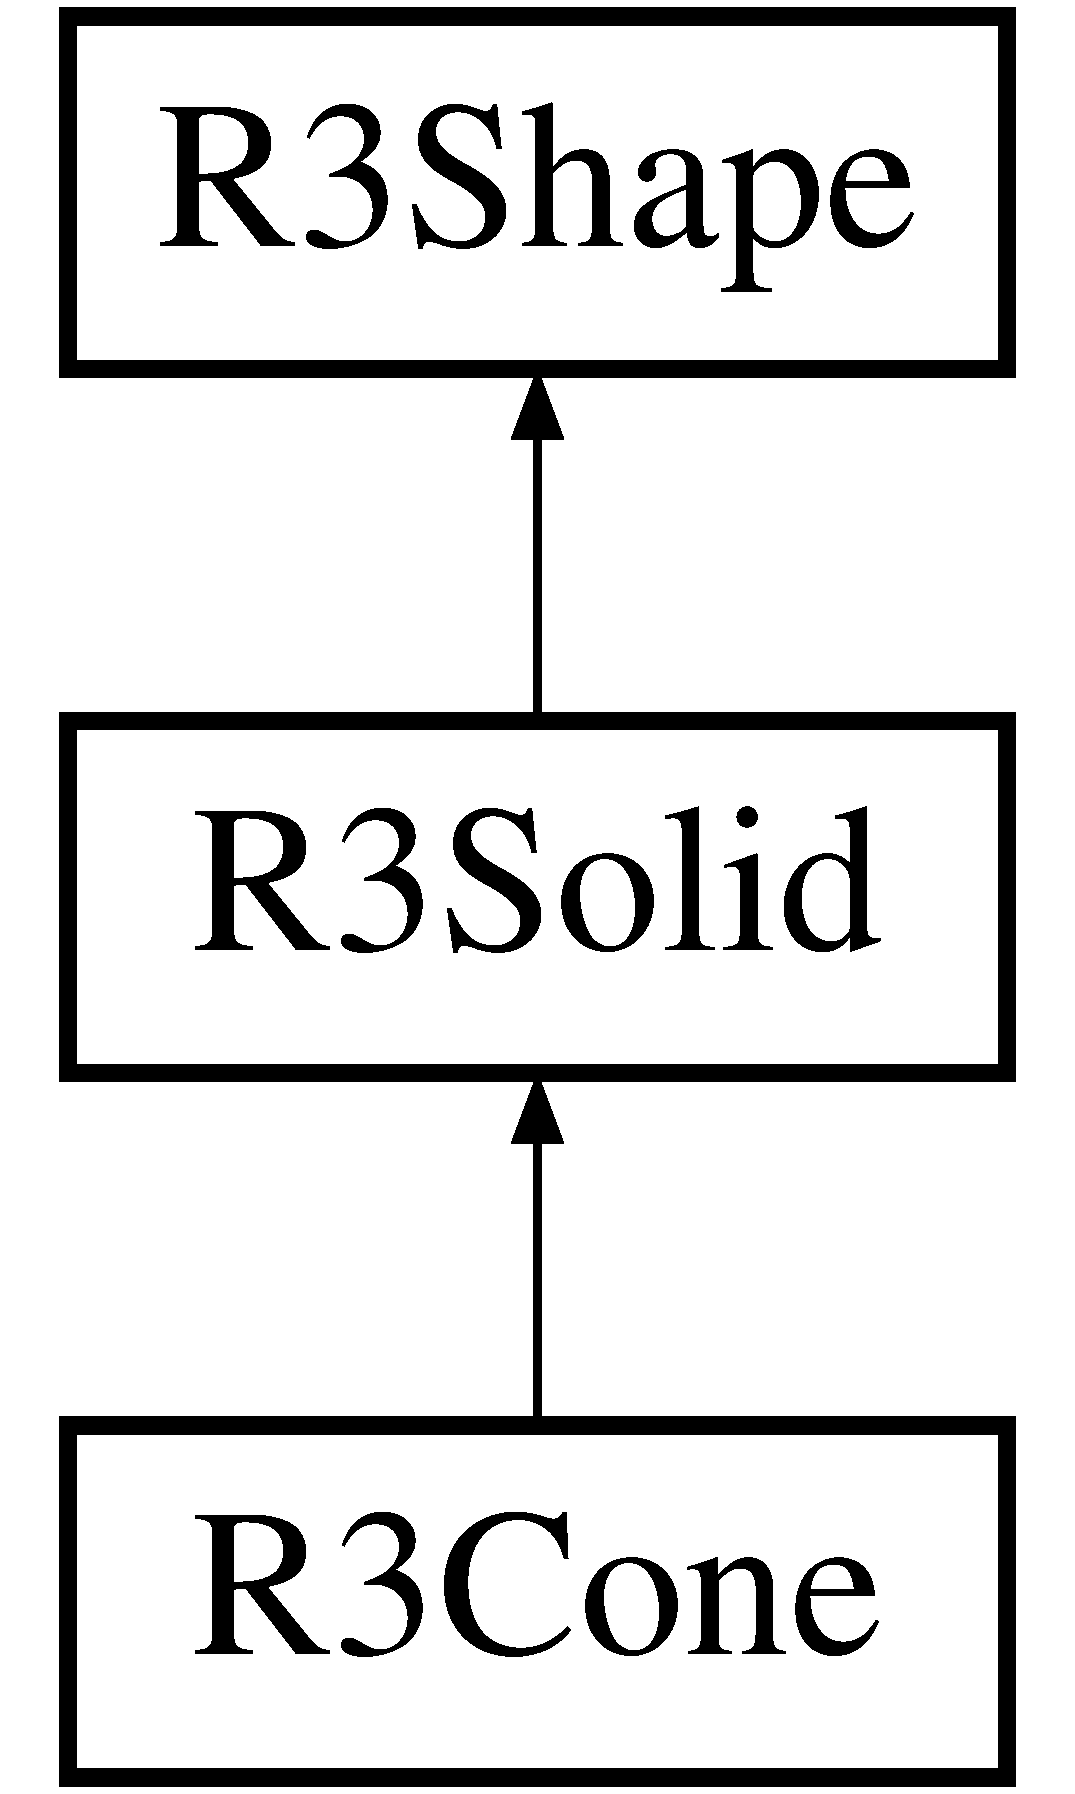
\includegraphics[height=3.000000cm]{class_r3_cone}
\end{center}
\end{figure}
\subsection*{Public Member Functions}
\begin{DoxyCompactItemize}
\item 
{\bfseries R3\+Cone} (const \hyperlink{class_r3_cone}{R3\+Cone} \&cone)\hypertarget{class_r3_cone_a2402226d1c55a351cf8f60427a503543}{}\label{class_r3_cone_a2402226d1c55a351cf8f60427a503543}

\item 
{\bfseries R3\+Cone} (const \hyperlink{class_r3_span}{R3\+Span} \&axis, R\+N\+Length radius)\hypertarget{class_r3_cone_a2368eaab7cdf8b154cb0e3b6a4151785}{}\label{class_r3_cone_a2368eaab7cdf8b154cb0e3b6a4151785}

\item 
{\bfseries R3\+Cone} (const \hyperlink{class_r3_point}{R3\+Point} \&p1, const \hyperlink{class_r3_point}{R3\+Point} \&p2, R\+N\+Length radius)\hypertarget{class_r3_cone_ab8563607c5b602c23e8e66092ccc4ac8}{}\label{class_r3_cone_ab8563607c5b602c23e8e66092ccc4ac8}

\item 
const \hyperlink{class_r3_point}{R3\+Point} \& {\bfseries Apex} (void) const \hypertarget{class_r3_cone_a55290a30b1f5b7737292d6523839254e}{}\label{class_r3_cone_a55290a30b1f5b7737292d6523839254e}

\item 
const \hyperlink{class_r3_span}{R3\+Span} \& {\bfseries Axis} (void) const \hypertarget{class_r3_cone_a42ad8d932f2921da7b89626c462895eb}{}\label{class_r3_cone_a42ad8d932f2921da7b89626c462895eb}

\item 
const \hyperlink{class_r3_circle}{R3\+Circle} \& {\bfseries Base} (void) const \hypertarget{class_r3_cone_a2932710d54570fd65907b8f1c18f3df9}{}\label{class_r3_cone_a2932710d54570fd65907b8f1c18f3df9}

\item 
const R\+N\+Length {\bfseries Radius} (void) const \hypertarget{class_r3_cone_a65de1e311cb0e9e80bb8b18888d6b4c8}{}\label{class_r3_cone_a65de1e311cb0e9e80bb8b18888d6b4c8}

\item 
const R\+N\+Length {\bfseries Height} (void) const \hypertarget{class_r3_cone_ab239ce5e790e1d5c45bcbc71e6bf77e1}{}\label{class_r3_cone_ab239ce5e790e1d5c45bcbc71e6bf77e1}

\item 
const R\+N\+Boolean {\bfseries Is\+Empty} (void) const \hypertarget{class_r3_cone_a4aac255739fac2f7c6e18410d8496ba8}{}\label{class_r3_cone_a4aac255739fac2f7c6e18410d8496ba8}

\item 
const R\+N\+Boolean {\bfseries Is\+Finite} (void) const \hypertarget{class_r3_cone_a9983889501dc296f35d9a8d601694531}{}\label{class_r3_cone_a9983889501dc296f35d9a8d601694531}

\item 
virtual const R\+N\+Boolean {\bfseries Is\+Point} (void) const \hypertarget{class_r3_cone_ac8b05cdf5dd4f9edb2b68fa11017df2b}{}\label{class_r3_cone_ac8b05cdf5dd4f9edb2b68fa11017df2b}

\item 
virtual const R\+N\+Boolean {\bfseries Is\+Linear} (void) const \hypertarget{class_r3_cone_a075a96de795eaa0bd7d45a76f6596b4f}{}\label{class_r3_cone_a075a96de795eaa0bd7d45a76f6596b4f}

\item 
virtual const R\+N\+Boolean {\bfseries Is\+Planar} (void) const \hypertarget{class_r3_cone_a56722672136a2d5c21834fb7a51a7e78}{}\label{class_r3_cone_a56722672136a2d5c21834fb7a51a7e78}

\item 
virtual const R\+N\+Boolean {\bfseries Is\+Convex} (void) const \hypertarget{class_r3_cone_a2ae431236f7fa452e185af5b2d0f08e7}{}\label{class_r3_cone_a2ae431236f7fa452e185af5b2d0f08e7}

\item 
virtual const \hyperlink{class_r_n_interval}{R\+N\+Interval} {\bfseries N\+Facets} (void) const \hypertarget{class_r3_cone_a180faf8a99d70e07a6d76386f8d8ee90}{}\label{class_r3_cone_a180faf8a99d70e07a6d76386f8d8ee90}

\item 
virtual const R\+N\+Area {\bfseries Area} (void) const \hypertarget{class_r3_cone_af81eded59a3b364cb13f78baee7b249c}{}\label{class_r3_cone_af81eded59a3b364cb13f78baee7b249c}

\item 
virtual const R\+N\+Volume {\bfseries Volume} (void) const \hypertarget{class_r3_cone_a3cbae8c4d70a7ba10fde06d0389fdad0}{}\label{class_r3_cone_a3cbae8c4d70a7ba10fde06d0389fdad0}

\item 
virtual const \hyperlink{class_r3_point}{R3\+Point} {\bfseries Centroid} (void) const \hypertarget{class_r3_cone_aa24c568fd2dd3e120ab6e926ad300631}{}\label{class_r3_cone_aa24c568fd2dd3e120ab6e926ad300631}

\item 
virtual const \hyperlink{class_r3_shape}{R3\+Shape} \& {\bfseries B\+Shape} (void) const \hypertarget{class_r3_cone_a1a270603a87b4eb9da930cce7d02233e}{}\label{class_r3_cone_a1a270603a87b4eb9da930cce7d02233e}

\item 
virtual const \hyperlink{class_r3_box}{R3\+Box} {\bfseries B\+Box} (void) const \hypertarget{class_r3_cone_a7e24a29083ef7405f4a2922a48642f05}{}\label{class_r3_cone_a7e24a29083ef7405f4a2922a48642f05}

\item 
virtual const \hyperlink{class_r3_sphere}{R3\+Sphere} {\bfseries B\+Sphere} (void) const \hypertarget{class_r3_cone_a8893fb2ca088972a847e835338af91a3}{}\label{class_r3_cone_a8893fb2ca088972a847e835338af91a3}

\item 
virtual void {\bfseries Empty} (void)\hypertarget{class_r3_cone_a3ccf2169c7d40f0c2949f670880ba070}{}\label{class_r3_cone_a3ccf2169c7d40f0c2949f670880ba070}

\item 
virtual void {\bfseries Translate} (const \hyperlink{class_r3_vector}{R3\+Vector} \&vector)\hypertarget{class_r3_cone_ace1d8f8c316b2ec9d207f15cf97eb4f2}{}\label{class_r3_cone_ace1d8f8c316b2ec9d207f15cf97eb4f2}

\item 
virtual void {\bfseries Reposition} (const \hyperlink{class_r3_span}{R3\+Span} \&span)\hypertarget{class_r3_cone_a0672a8f33cc1e5af79916d16bf225132}{}\label{class_r3_cone_a0672a8f33cc1e5af79916d16bf225132}

\item 
virtual void {\bfseries Resize} (R\+N\+Length radius)\hypertarget{class_r3_cone_a33cee7827565fdc523c03b885671a938}{}\label{class_r3_cone_a33cee7827565fdc523c03b885671a938}

\item 
virtual void {\bfseries Transform} (const \hyperlink{class_r3_transformation}{R3\+Transformation} \&transformation)\hypertarget{class_r3_cone_a513ec910f071fd192b499585cc0f4dbc}{}\label{class_r3_cone_a513ec910f071fd192b499585cc0f4dbc}

\item 
virtual void {\bfseries Draw} (const \hyperlink{class_r_n_flags}{R3\+Draw\+Flags} draw\+\_\+flags=R3\+\_\+\+D\+E\+F\+A\+U\+L\+T\+\_\+\+D\+R\+A\+W\+\_\+\+F\+L\+A\+GS) const \hypertarget{class_r3_cone_a04da8954c8c2519b6873eb14d3cafa14}{}\label{class_r3_cone_a04da8954c8c2519b6873eb14d3cafa14}

\item 
R\+N\+Boolean {\bfseries operator==} (const \hyperlink{class_r3_cone}{R3\+Cone} \&cone) const \hypertarget{class_r3_cone_ace8b3fae2b4d609b43a7ac56cc36fcaa}{}\label{class_r3_cone_ace8b3fae2b4d609b43a7ac56cc36fcaa}

\item 
R\+N\+Boolean {\bfseries operator!=} (const \hyperlink{class_r3_cone}{R3\+Cone} \&cone) const \hypertarget{class_r3_cone_ab1804af6cdd07425c2e4c45f73a01814}{}\label{class_r3_cone_ab1804af6cdd07425c2e4c45f73a01814}

\item 
{\bfseries R\+N\+\_\+\+C\+L\+A\+S\+S\+\_\+\+T\+Y\+P\+E\+\_\+\+D\+E\+C\+L\+A\+R\+A\+T\+I\+O\+NS} (\hyperlink{class_r3_cone}{R3\+Cone})\hypertarget{class_r3_cone_a3b15944433f541ec231912600913f6ee}{}\label{class_r3_cone_a3b15944433f541ec231912600913f6ee}

\item 
{\bfseries R3\+\_\+\+S\+H\+A\+P\+E\+\_\+\+R\+E\+L\+A\+T\+I\+O\+N\+S\+H\+I\+P\+\_\+\+D\+E\+C\+L\+A\+R\+A\+T\+I\+O\+NS} (\hyperlink{class_r3_cone}{R3\+Cone})\hypertarget{class_r3_cone_a768031b88b4c08289529c0d56e479c4a}{}\label{class_r3_cone_a768031b88b4c08289529c0d56e479c4a}

\end{DoxyCompactItemize}


The documentation for this class was generated from the following files\+:\begin{DoxyCompactItemize}
\item 
R3\+Shapes/R3\+Cone.\+h\item 
R3\+Shapes/R3\+Cone.\+cpp\item 
R3\+Shapes/R3\+Draw.\+cpp\end{DoxyCompactItemize}

\hypertarget{class_r3_coord_system}{}\section{R3\+Coord\+System Class Reference}
\label{class_r3_coord_system}\index{R3\+Coord\+System@{R3\+Coord\+System}}
\subsection*{Public Member Functions}
\begin{DoxyCompactItemize}
\item 
{\bfseries R3\+Coord\+System} (const \hyperlink{class_r3_coord_system}{R3\+Coord\+System} \&cs)\hypertarget{class_r3_coord_system_ad647b5403983e64cd4d820e16e360ed3}{}\label{class_r3_coord_system_ad647b5403983e64cd4d820e16e360ed3}

\item 
{\bfseries R3\+Coord\+System} (const \hyperlink{class_r3_point}{R3\+Point} \&origin, const \hyperlink{class_r3_triad}{R3\+Triad} \&axes)\hypertarget{class_r3_coord_system_a57a0e0568d208718e5d6de97f5beb33b}{}\label{class_r3_coord_system_a57a0e0568d208718e5d6de97f5beb33b}

\item 
const \hyperlink{class_r3_point}{R3\+Point} \& {\bfseries Origin} (void) const \hypertarget{class_r3_coord_system_ad85af546d276d612df7582a5bb0cbefe}{}\label{class_r3_coord_system_ad85af546d276d612df7582a5bb0cbefe}

\item 
const \hyperlink{class_r3_triad}{R3\+Triad} \& {\bfseries Axes} (void) const \hypertarget{class_r3_coord_system_aeedd0f58c504b073b48c13d36dd75ceb}{}\label{class_r3_coord_system_aeedd0f58c504b073b48c13d36dd75ceb}

\item 
const \hyperlink{class_r4_matrix}{R4\+Matrix} {\bfseries Matrix} (void) const \hypertarget{class_r3_coord_system_af0adfc1c024c716dff7638b4d509ebe7}{}\label{class_r3_coord_system_af0adfc1c024c716dff7638b4d509ebe7}

\item 
const \hyperlink{class_r4_matrix}{R4\+Matrix} {\bfseries Inverse\+Matrix} (void) const \hypertarget{class_r3_coord_system_ad2c0f30ab28e7d2668095aae27527116}{}\label{class_r3_coord_system_ad2c0f30ab28e7d2668095aae27527116}

\item 
const R\+N\+Boolean {\bfseries operator==} (const \hyperlink{class_r3_coord_system}{R3\+Coord\+System} \&cs) const \hypertarget{class_r3_coord_system_a03e0943ab70ae065801dc098518e0d37}{}\label{class_r3_coord_system_a03e0943ab70ae065801dc098518e0d37}

\item 
const R\+N\+Boolean {\bfseries operator!=} (const \hyperlink{class_r3_coord_system}{R3\+Coord\+System} \&cs) const \hypertarget{class_r3_coord_system_a8e3967c05596699fb05091eed1dea4a8}{}\label{class_r3_coord_system_a8e3967c05596699fb05091eed1dea4a8}

\item 
void {\bfseries Translate} (const \hyperlink{class_r3_vector}{R3\+Vector} \&offset)\hypertarget{class_r3_coord_system_a39a2e90a2876ad1083d7f642f2bc8069}{}\label{class_r3_coord_system_a39a2e90a2876ad1083d7f642f2bc8069}

\item 
void {\bfseries Rotate} (R\+N\+Axis axis, R\+N\+Angle radians)\hypertarget{class_r3_coord_system_a193f198655ecf24f732c1a5c62fecae5}{}\label{class_r3_coord_system_a193f198655ecf24f732c1a5c62fecae5}

\item 
void {\bfseries Rotate} (const \hyperlink{class_r3_vector}{R3\+Vector} \&axis, R\+N\+Angle radians)\hypertarget{class_r3_coord_system_a8deb9d70f2988c8546f7eb8d1d8fa79a}{}\label{class_r3_coord_system_a8deb9d70f2988c8546f7eb8d1d8fa79a}

\item 
void {\bfseries Rotate} (const \hyperlink{class_r3_vector}{R3\+Vector} \&from, const \hyperlink{class_r3_vector}{R3\+Vector} \&to)\hypertarget{class_r3_coord_system_a7a9884824e05db619d60a15a07477f7b}{}\label{class_r3_coord_system_a7a9884824e05db619d60a15a07477f7b}

\item 
void {\bfseries Mirror} (const \hyperlink{class_r3_plane}{R3\+Plane} \&plane)\hypertarget{class_r3_coord_system_aadf326f5739fbcf12433696828c57115}{}\label{class_r3_coord_system_aadf326f5739fbcf12433696828c57115}

\item 
void {\bfseries Transform} (const \hyperlink{class_r3_transformation}{R3\+Transformation} \&transformation)\hypertarget{class_r3_coord_system_a52d42142e50b89a4a68341c1e3786bc6}{}\label{class_r3_coord_system_a52d42142e50b89a4a68341c1e3786bc6}

\item 
void {\bfseries Inverse\+Transform} (const \hyperlink{class_r3_transformation}{R3\+Transformation} \&transformation)\hypertarget{class_r3_coord_system_a2aa0a170c4879816b666fdb4cbfeb48a}{}\label{class_r3_coord_system_a2aa0a170c4879816b666fdb4cbfeb48a}

\item 
void {\bfseries Set\+Origin} (const \hyperlink{class_r3_point}{R3\+Point} \&origin)\hypertarget{class_r3_coord_system_a1285c003973202ae8f8e7a27bab659f5}{}\label{class_r3_coord_system_a1285c003973202ae8f8e7a27bab659f5}

\item 
void {\bfseries Set\+Axes} (const \hyperlink{class_r3_triad}{R3\+Triad} \&axes)\hypertarget{class_r3_coord_system_a3a53c0860ab32624dca0666797ef1923}{}\label{class_r3_coord_system_a3a53c0860ab32624dca0666797ef1923}

\item 
void {\bfseries Reset} (const \hyperlink{class_r3_point}{R3\+Point} \&origin, const \hyperlink{class_r3_triad}{R3\+Triad} \&axes)\hypertarget{class_r3_coord_system_a3173288920cf32f9712ecb7c4d6bbba7}{}\label{class_r3_coord_system_a3173288920cf32f9712ecb7c4d6bbba7}

\item 
void {\bfseries Draw} (void) const \hypertarget{class_r3_coord_system_a406ed7229477458b3403b56315c8de01}{}\label{class_r3_coord_system_a406ed7229477458b3403b56315c8de01}

\item 
void {\bfseries Outline} (void) const \hypertarget{class_r3_coord_system_a5fbef1883ae00e9156f2a32943007081}{}\label{class_r3_coord_system_a5fbef1883ae00e9156f2a32943007081}

\end{DoxyCompactItemize}


The documentation for this class was generated from the following files\+:\begin{DoxyCompactItemize}
\item 
R3\+Shapes/R3\+Crdsys.\+h\item 
R3\+Shapes/R3\+Crdsys.\+cpp\item 
R3\+Shapes/R3\+Draw.\+cpp\end{DoxyCompactItemize}

\hypertarget{class_r3_cylinder}{}\section{R3\+Cylinder Class Reference}
\label{class_r3_cylinder}\index{R3\+Cylinder@{R3\+Cylinder}}
Inheritance diagram for R3\+Cylinder\+:\begin{figure}[H]
\begin{center}
\leavevmode
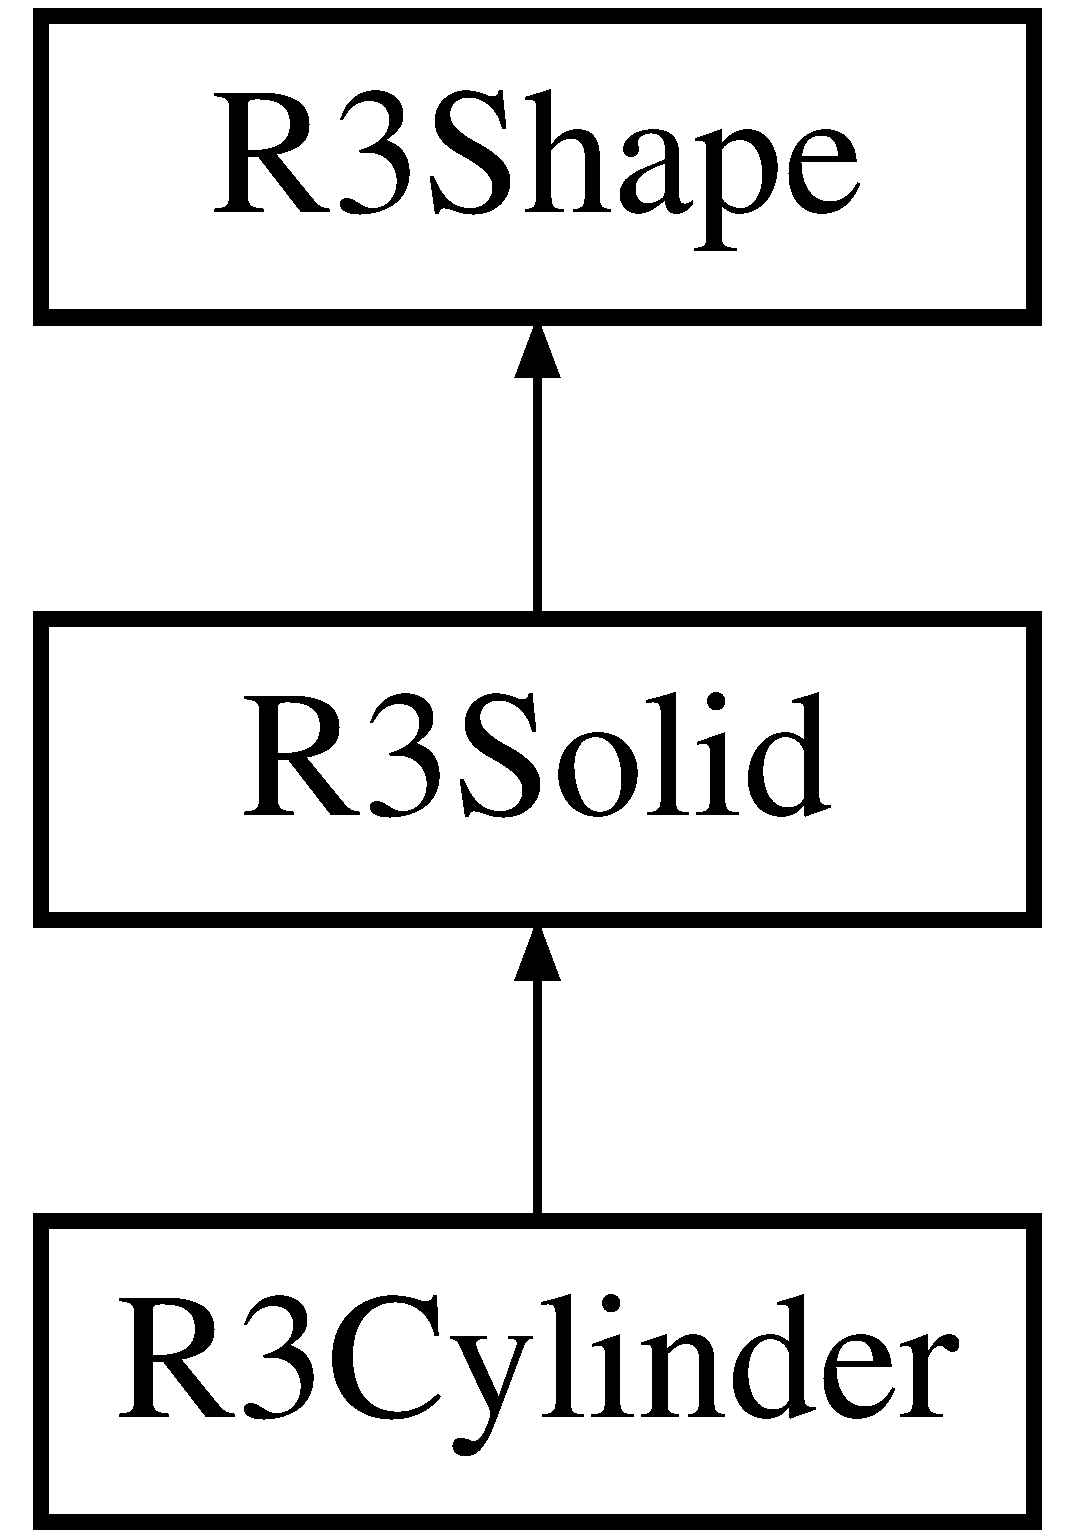
\includegraphics[height=3.000000cm]{class_r3_cylinder}
\end{center}
\end{figure}
\subsection*{Public Member Functions}
\begin{DoxyCompactItemize}
\item 
{\bfseries R3\+Cylinder} (const \hyperlink{class_r3_cylinder}{R3\+Cylinder} \&cylinder)\hypertarget{class_r3_cylinder_a2f7720cfcb923aeefda8ab987f2c3613}{}\label{class_r3_cylinder_a2f7720cfcb923aeefda8ab987f2c3613}

\item 
{\bfseries R3\+Cylinder} (const \hyperlink{class_r3_span}{R3\+Span} \&axis, R\+N\+Length radius)\hypertarget{class_r3_cylinder_a74060d68ff772137a5959605dbc9a85c}{}\label{class_r3_cylinder_a74060d68ff772137a5959605dbc9a85c}

\item 
{\bfseries R3\+Cylinder} (const \hyperlink{class_r3_point}{R3\+Point} \&p1, const \hyperlink{class_r3_point}{R3\+Point} \&p2, R\+N\+Length radius)\hypertarget{class_r3_cylinder_ab534885f3e5b74922e483b6cccad50d7}{}\label{class_r3_cylinder_ab534885f3e5b74922e483b6cccad50d7}

\item 
const \hyperlink{class_r3_span}{R3\+Span} \& {\bfseries Axis} (void) const \hypertarget{class_r3_cylinder_af9713e6727376ad7b36609b7630f0474}{}\label{class_r3_cylinder_af9713e6727376ad7b36609b7630f0474}

\item 
const \hyperlink{class_r3_circle}{R3\+Circle} \& {\bfseries Base} (void) const \hypertarget{class_r3_cylinder_a7f7aec4a4ad963824866cc7c9d577ae5}{}\label{class_r3_cylinder_a7f7aec4a4ad963824866cc7c9d577ae5}

\item 
const \hyperlink{class_r3_circle}{R3\+Circle} \& {\bfseries Top} (void) const \hypertarget{class_r3_cylinder_a021176baa6fde6f8b217da7c92be5835}{}\label{class_r3_cylinder_a021176baa6fde6f8b217da7c92be5835}

\item 
const R\+N\+Length {\bfseries Radius} (void) const \hypertarget{class_r3_cylinder_aa021a3ad2508da849ddff73ca89b65e8}{}\label{class_r3_cylinder_aa021a3ad2508da849ddff73ca89b65e8}

\item 
const R\+N\+Length {\bfseries Height} (void) const \hypertarget{class_r3_cylinder_a4cbde13d0de53b95342ddc7f884a4422}{}\label{class_r3_cylinder_a4cbde13d0de53b95342ddc7f884a4422}

\item 
const R\+N\+Boolean {\bfseries Is\+Empty} (void) const \hypertarget{class_r3_cylinder_a761d0c4aa5d83fc0affb7900b9805c8d}{}\label{class_r3_cylinder_a761d0c4aa5d83fc0affb7900b9805c8d}

\item 
const R\+N\+Boolean {\bfseries Is\+Finite} (void) const \hypertarget{class_r3_cylinder_a0280a087f4ffa522034a1ded3eeaad39}{}\label{class_r3_cylinder_a0280a087f4ffa522034a1ded3eeaad39}

\item 
virtual const R\+N\+Boolean {\bfseries Is\+Point} (void) const \hypertarget{class_r3_cylinder_a202a19364df59cbf2701c12f7ce8e13e}{}\label{class_r3_cylinder_a202a19364df59cbf2701c12f7ce8e13e}

\item 
virtual const R\+N\+Boolean {\bfseries Is\+Linear} (void) const \hypertarget{class_r3_cylinder_a05ee53382da321aa30bf2e61ccabbd49}{}\label{class_r3_cylinder_a05ee53382da321aa30bf2e61ccabbd49}

\item 
virtual const R\+N\+Boolean {\bfseries Is\+Planar} (void) const \hypertarget{class_r3_cylinder_a151f912edac18094583a02526a2198e6}{}\label{class_r3_cylinder_a151f912edac18094583a02526a2198e6}

\item 
virtual const R\+N\+Boolean {\bfseries Is\+Convex} (void) const \hypertarget{class_r3_cylinder_a15588c963e1b0d27483a700cc1cb5656}{}\label{class_r3_cylinder_a15588c963e1b0d27483a700cc1cb5656}

\item 
virtual const \hyperlink{class_r_n_interval}{R\+N\+Interval} {\bfseries N\+Facets} (void) const \hypertarget{class_r3_cylinder_a7d344fcfb80a822a767b77155b4d9399}{}\label{class_r3_cylinder_a7d344fcfb80a822a767b77155b4d9399}

\item 
virtual const R\+N\+Area {\bfseries Area} (void) const \hypertarget{class_r3_cylinder_a72b96706097f7c706290b62051df6b69}{}\label{class_r3_cylinder_a72b96706097f7c706290b62051df6b69}

\item 
virtual const R\+N\+Volume {\bfseries Volume} (void) const \hypertarget{class_r3_cylinder_a42968df3e8bdcb0a06bf8f5fe5e1987a}{}\label{class_r3_cylinder_a42968df3e8bdcb0a06bf8f5fe5e1987a}

\item 
virtual const \hyperlink{class_r3_point}{R3\+Point} {\bfseries Centroid} (void) const \hypertarget{class_r3_cylinder_aad3d64e44f52155c06114445dbf8a0c4}{}\label{class_r3_cylinder_aad3d64e44f52155c06114445dbf8a0c4}

\item 
virtual const \hyperlink{class_r3_shape}{R3\+Shape} \& {\bfseries B\+Shape} (void) const \hypertarget{class_r3_cylinder_aa736079c814e29277370e02d13c9d9a4}{}\label{class_r3_cylinder_aa736079c814e29277370e02d13c9d9a4}

\item 
virtual const \hyperlink{class_r3_box}{R3\+Box} {\bfseries B\+Box} (void) const \hypertarget{class_r3_cylinder_afbbf0f01b24e42d9db5f4ec5d1269004}{}\label{class_r3_cylinder_afbbf0f01b24e42d9db5f4ec5d1269004}

\item 
virtual const \hyperlink{class_r3_sphere}{R3\+Sphere} {\bfseries B\+Sphere} (void) const \hypertarget{class_r3_cylinder_ac97df50f5f48cd7a444ac80dc1ea4054}{}\label{class_r3_cylinder_ac97df50f5f48cd7a444ac80dc1ea4054}

\item 
virtual void {\bfseries Empty} (void)\hypertarget{class_r3_cylinder_ab8fce3ce06bd641b3848c043fed0388e}{}\label{class_r3_cylinder_ab8fce3ce06bd641b3848c043fed0388e}

\item 
virtual void {\bfseries Translate} (const \hyperlink{class_r3_vector}{R3\+Vector} \&vector)\hypertarget{class_r3_cylinder_ae7ecfdd8c99f067d82b3020e07ee34ff}{}\label{class_r3_cylinder_ae7ecfdd8c99f067d82b3020e07ee34ff}

\item 
virtual void {\bfseries Reposition} (const \hyperlink{class_r3_span}{R3\+Span} \&span)\hypertarget{class_r3_cylinder_a783f9746c9ba0cb0d051a57c335d0c54}{}\label{class_r3_cylinder_a783f9746c9ba0cb0d051a57c335d0c54}

\item 
virtual void {\bfseries Resize} (R\+N\+Length radius)\hypertarget{class_r3_cylinder_af4deec6d1807b9a294197e1f3d9e079f}{}\label{class_r3_cylinder_af4deec6d1807b9a294197e1f3d9e079f}

\item 
virtual void {\bfseries Transform} (const \hyperlink{class_r3_transformation}{R3\+Transformation} \&transformation)\hypertarget{class_r3_cylinder_a3143c31494229b9883b044ae6bfdde00}{}\label{class_r3_cylinder_a3143c31494229b9883b044ae6bfdde00}

\item 
virtual void {\bfseries Draw} (const \hyperlink{class_r_n_flags}{R3\+Draw\+Flags} draw\+\_\+flags=R3\+\_\+\+D\+E\+F\+A\+U\+L\+T\+\_\+\+D\+R\+A\+W\+\_\+\+F\+L\+A\+GS) const \hypertarget{class_r3_cylinder_a435b3dbe6d558cbdeeaa21ddf4181c76}{}\label{class_r3_cylinder_a435b3dbe6d558cbdeeaa21ddf4181c76}

\item 
R\+N\+Boolean {\bfseries operator==} (const \hyperlink{class_r3_cylinder}{R3\+Cylinder} \&cylinder) const \hypertarget{class_r3_cylinder_a2015f59fdb62b8d72f11d54d9416e76e}{}\label{class_r3_cylinder_a2015f59fdb62b8d72f11d54d9416e76e}

\item 
R\+N\+Boolean {\bfseries operator!=} (const \hyperlink{class_r3_cylinder}{R3\+Cylinder} \&cylinder) const \hypertarget{class_r3_cylinder_ab06c3455590a4ad96444c525343d2c8a}{}\label{class_r3_cylinder_ab06c3455590a4ad96444c525343d2c8a}

\item 
{\bfseries R\+N\+\_\+\+C\+L\+A\+S\+S\+\_\+\+T\+Y\+P\+E\+\_\+\+D\+E\+C\+L\+A\+R\+A\+T\+I\+O\+NS} (\hyperlink{class_r3_cylinder}{R3\+Cylinder})\hypertarget{class_r3_cylinder_a17cc7c2ee0df53862f35fd121afa4356}{}\label{class_r3_cylinder_a17cc7c2ee0df53862f35fd121afa4356}

\item 
{\bfseries R3\+\_\+\+S\+H\+A\+P\+E\+\_\+\+R\+E\+L\+A\+T\+I\+O\+N\+S\+H\+I\+P\+\_\+\+D\+E\+C\+L\+A\+R\+A\+T\+I\+O\+NS} (\hyperlink{class_r3_cylinder}{R3\+Cylinder})\hypertarget{class_r3_cylinder_aec5c68c5cb265a56e201dd56451b8696}{}\label{class_r3_cylinder_aec5c68c5cb265a56e201dd56451b8696}

\end{DoxyCompactItemize}


The documentation for this class was generated from the following files\+:\begin{DoxyCompactItemize}
\item 
R3\+Shapes/R3\+Cylinder.\+h\item 
R3\+Shapes/R3\+Cylinder.\+cpp\item 
R3\+Shapes/R3\+Draw.\+cpp\end{DoxyCompactItemize}

\hypertarget{class_r3_directional_light}{}\section{R3\+Directional\+Light Class Reference}
\label{class_r3_directional_light}\index{R3\+Directional\+Light@{R3\+Directional\+Light}}
Inheritance diagram for R3\+Directional\+Light\+:\begin{figure}[H]
\begin{center}
\leavevmode
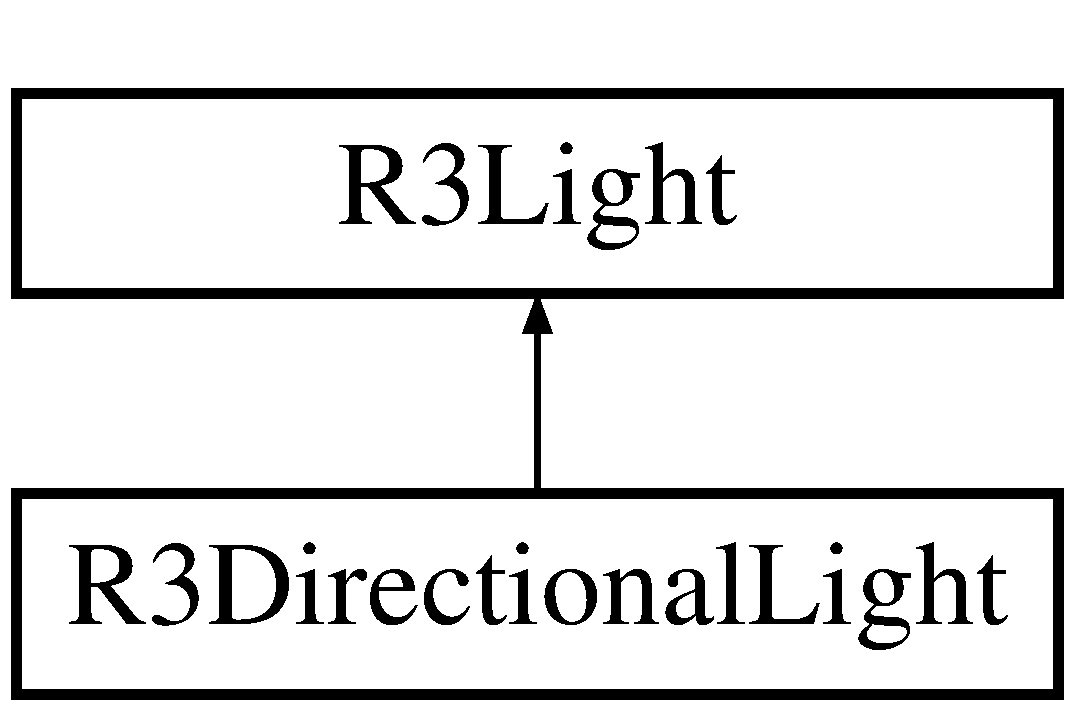
\includegraphics[height=2.000000cm]{class_r3_directional_light}
\end{center}
\end{figure}
\subsection*{Public Member Functions}
\begin{DoxyCompactItemize}
\item 
{\bfseries R3\+Directional\+Light} (const \hyperlink{class_r3_directional_light}{R3\+Directional\+Light} \&light)\hypertarget{class_r3_directional_light_a3e6d46f777599f81aac7ae38e0c07e5e}{}\label{class_r3_directional_light_a3e6d46f777599f81aac7ae38e0c07e5e}

\item 
{\bfseries R3\+Directional\+Light} (const \hyperlink{class_r3_vector}{R3\+Vector} \&direction, const \hyperlink{class_r_n_rgb}{R\+N\+Rgb} \&color, R\+N\+Scalar intensity=1.\+0, R\+N\+Boolean active=T\+R\+UE)\hypertarget{class_r3_directional_light_a79bb3a777e09a75d15b0132f3b31f749}{}\label{class_r3_directional_light_a79bb3a777e09a75d15b0132f3b31f749}

\item 
const \hyperlink{class_r3_vector}{R3\+Vector} \& {\bfseries Direction} (void) const \hypertarget{class_r3_directional_light_a3fb1dccde87ac9a7fded9b4c217ae9c3}{}\label{class_r3_directional_light_a3fb1dccde87ac9a7fded9b4c217ae9c3}

\item 
virtual void {\bfseries Set\+Direction} (const \hyperlink{class_r3_vector}{R3\+Vector} \&direction)\hypertarget{class_r3_directional_light_a1f7a22adaf5c48af06b4fd2c985c6a14}{}\label{class_r3_directional_light_a1f7a22adaf5c48af06b4fd2c985c6a14}

\item 
virtual \hyperlink{class_r_n_rgb}{R\+N\+Rgb} {\bfseries Reflection} (const \hyperlink{class_r3_brdf}{R3\+Brdf} \&brdf, const \hyperlink{class_r3_point}{R3\+Point} \&eye, const \hyperlink{class_r3_point}{R3\+Point} \&point, const \hyperlink{class_r3_vector}{R3\+Vector} \&normal) const \hypertarget{class_r3_directional_light_a3da3213d3fd501ede4401268668ef21e}{}\label{class_r3_directional_light_a3da3213d3fd501ede4401268668ef21e}

\item 
virtual \hyperlink{class_r_n_rgb}{R\+N\+Rgb} {\bfseries Diffuse\+Reflection} (const \hyperlink{class_r3_brdf}{R3\+Brdf} \&brdf, const \hyperlink{class_r3_point}{R3\+Point} \&point, const \hyperlink{class_r3_vector}{R3\+Vector} \&normal) const \hypertarget{class_r3_directional_light_ac415af4ae765d59535cddd842df422ab}{}\label{class_r3_directional_light_ac415af4ae765d59535cddd842df422ab}

\item 
virtual \hyperlink{class_r_n_rgb}{R\+N\+Rgb} {\bfseries Specular\+Reflection} (const \hyperlink{class_r3_brdf}{R3\+Brdf} \&brdf, const \hyperlink{class_r3_point}{R3\+Point} \&eye, const \hyperlink{class_r3_point}{R3\+Point} \&point, const \hyperlink{class_r3_vector}{R3\+Vector} \&normal) const \hypertarget{class_r3_directional_light_a6753359b3f43ab8f5964b2b7a0ab8522}{}\label{class_r3_directional_light_a6753359b3f43ab8f5964b2b7a0ab8522}

\item 
virtual void {\bfseries Draw} (int i) const \hypertarget{class_r3_directional_light_a8a18993a1898af3fc05ffc78a7c469c1}{}\label{class_r3_directional_light_a8a18993a1898af3fc05ffc78a7c469c1}

\item 
{\bfseries R\+N\+\_\+\+C\+L\+A\+S\+S\+\_\+\+T\+Y\+P\+E\+\_\+\+D\+E\+C\+L\+A\+R\+A\+T\+I\+O\+NS} (\hyperlink{class_r3_directional_light}{R3\+Directional\+Light})\hypertarget{class_r3_directional_light_a6fbdaa386aeb812baa309038766993dc}{}\label{class_r3_directional_light_a6fbdaa386aeb812baa309038766993dc}

\end{DoxyCompactItemize}


The documentation for this class was generated from the following files\+:\begin{DoxyCompactItemize}
\item 
R3\+Graphics/R3\+Directional\+Light.\+h\item 
R3\+Graphics/R3\+Directional\+Light.\+cpp\end{DoxyCompactItemize}

\hypertarget{class_r3_ellipse}{}\section{R3\+Ellipse Class Reference}
\label{class_r3_ellipse}\index{R3\+Ellipse@{R3\+Ellipse}}
Inheritance diagram for R3\+Ellipse\+:\begin{figure}[H]
\begin{center}
\leavevmode
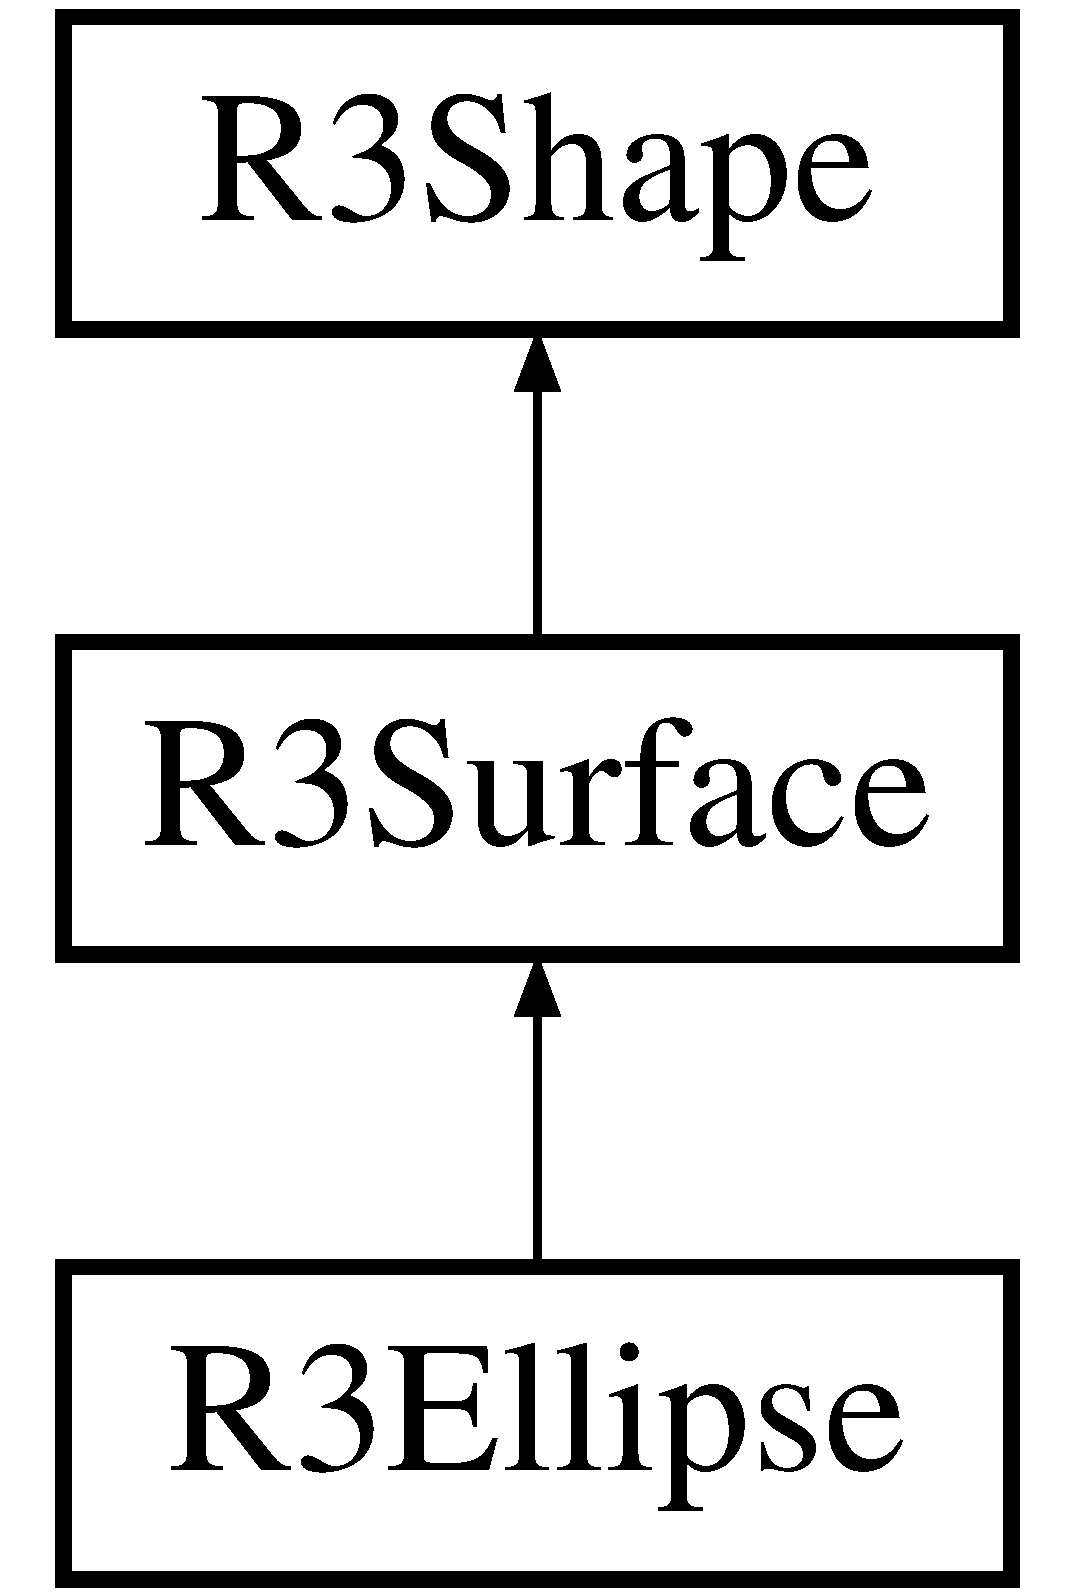
\includegraphics[height=3.000000cm]{class_r3_ellipse}
\end{center}
\end{figure}
\subsection*{Public Member Functions}
\begin{DoxyCompactItemize}
\item 
{\bfseries R3\+Ellipse} (const \hyperlink{class_r3_ellipse}{R3\+Ellipse} \&ellipse)\hypertarget{class_r3_ellipse_aaf748d31d339d6c51c69e9688354e59d}{}\label{class_r3_ellipse_aaf748d31d339d6c51c69e9688354e59d}

\item 
{\bfseries R3\+Ellipse} (const \hyperlink{class_r3_coord_system}{R3\+Coord\+System} \&cs, const \hyperlink{class_r2_vector}{R2\+Vector} \&radii)\hypertarget{class_r3_ellipse_a6ce0984c938c2f9a8516e7c77ff6db31}{}\label{class_r3_ellipse_a6ce0984c938c2f9a8516e7c77ff6db31}

\item 
const \hyperlink{class_r3_point}{R3\+Point} \& {\bfseries Center} (void) const \hypertarget{class_r3_ellipse_afbc3d4aa4dddf17cbf420b6c0207e07c}{}\label{class_r3_ellipse_afbc3d4aa4dddf17cbf420b6c0207e07c}

\item 
const \hyperlink{class_r2_vector}{R2\+Vector} \& {\bfseries Radii} (void) const \hypertarget{class_r3_ellipse_a4044585c29d11fa22eeadff4063f768d}{}\label{class_r3_ellipse_a4044585c29d11fa22eeadff4063f768d}

\item 
const \hyperlink{class_r3_plane}{R3\+Plane} {\bfseries Plane} (void) const \hypertarget{class_r3_ellipse_a6ef1f883a52a989779ef53d9c7c13511}{}\label{class_r3_ellipse_a6ef1f883a52a989779ef53d9c7c13511}

\item 
const \hyperlink{class_r3_vector}{R3\+Vector} \& {\bfseries Normal} (void) const \hypertarget{class_r3_ellipse_ada50c9633f6a4e045fb064636d8057e4}{}\label{class_r3_ellipse_ada50c9633f6a4e045fb064636d8057e4}

\item 
const R\+N\+Boolean {\bfseries Is\+Empty} (void) const \hypertarget{class_r3_ellipse_a31b818bab4af14a23271c79fa75f039c}{}\label{class_r3_ellipse_a31b818bab4af14a23271c79fa75f039c}

\item 
const R\+N\+Boolean {\bfseries Is\+Finite} (void) const \hypertarget{class_r3_ellipse_a15820e409d1ed71c33f97ce535a75df7}{}\label{class_r3_ellipse_a15820e409d1ed71c33f97ce535a75df7}

\item 
virtual const R\+N\+Boolean {\bfseries Is\+Point} (void) const \hypertarget{class_r3_ellipse_a7ab39e725683da3dd47028f608762b2d}{}\label{class_r3_ellipse_a7ab39e725683da3dd47028f608762b2d}

\item 
virtual const R\+N\+Boolean {\bfseries Is\+Linear} (void) const \hypertarget{class_r3_ellipse_a058964b90e84e8509863e2c55d72786f}{}\label{class_r3_ellipse_a058964b90e84e8509863e2c55d72786f}

\item 
virtual const R\+N\+Boolean {\bfseries Is\+Planar} (void) const \hypertarget{class_r3_ellipse_a8f603317f1793654f4bf072ef9d7822c}{}\label{class_r3_ellipse_a8f603317f1793654f4bf072ef9d7822c}

\item 
virtual const R\+N\+Boolean {\bfseries Is\+Convex} (void) const \hypertarget{class_r3_ellipse_af44ed227c06af897fd63861c558163cf}{}\label{class_r3_ellipse_af44ed227c06af897fd63861c558163cf}

\item 
virtual const \hyperlink{class_r_n_interval}{R\+N\+Interval} {\bfseries N\+Facets} (void) const \hypertarget{class_r3_ellipse_a149dc39dbcf239ef8bdc131245fcd6bb}{}\label{class_r3_ellipse_a149dc39dbcf239ef8bdc131245fcd6bb}

\item 
virtual const R\+N\+Area {\bfseries Area} (void) const \hypertarget{class_r3_ellipse_a9b80af9e9f6f2f4c3bc4a4546865fd63}{}\label{class_r3_ellipse_a9b80af9e9f6f2f4c3bc4a4546865fd63}

\item 
virtual const \hyperlink{class_r3_point}{R3\+Point} {\bfseries Centroid} (void) const \hypertarget{class_r3_ellipse_a971f3eee289e4c8368385389caa66fd2}{}\label{class_r3_ellipse_a971f3eee289e4c8368385389caa66fd2}

\item 
virtual const \hyperlink{class_r3_shape}{R3\+Shape} \& {\bfseries B\+Shape} (void) const \hypertarget{class_r3_ellipse_af8e1c0624f2896afa7aca0325e4814fa}{}\label{class_r3_ellipse_af8e1c0624f2896afa7aca0325e4814fa}

\item 
virtual const \hyperlink{class_r3_box}{R3\+Box} {\bfseries B\+Box} (void) const \hypertarget{class_r3_ellipse_a87b2311cab38a65840f4de230992e274}{}\label{class_r3_ellipse_a87b2311cab38a65840f4de230992e274}

\item 
virtual const \hyperlink{class_r3_sphere}{R3\+Sphere} {\bfseries B\+Sphere} (void) const \hypertarget{class_r3_ellipse_a907acd1e0d751bf830ac5c5450ff3631}{}\label{class_r3_ellipse_a907acd1e0d751bf830ac5c5450ff3631}

\item 
virtual void {\bfseries Flip} (void)\hypertarget{class_r3_ellipse_a369f5fbb7ba3a4dd5f4c1c080bb01b8e}{}\label{class_r3_ellipse_a369f5fbb7ba3a4dd5f4c1c080bb01b8e}

\item 
virtual void {\bfseries Empty} (void)\hypertarget{class_r3_ellipse_a6889ccaf530bbdd1fd15e91a077d7a63}{}\label{class_r3_ellipse_a6889ccaf530bbdd1fd15e91a077d7a63}

\item 
virtual void {\bfseries Translate} (const \hyperlink{class_r3_vector}{R3\+Vector} \&vector)\hypertarget{class_r3_ellipse_a3a23e824f5e03ae03b4da1110535ab4b}{}\label{class_r3_ellipse_a3a23e824f5e03ae03b4da1110535ab4b}

\item 
virtual void {\bfseries Reposition} (const \hyperlink{class_r3_point}{R3\+Point} \&center)\hypertarget{class_r3_ellipse_aacb7dab591134033f037114f816f274a}{}\label{class_r3_ellipse_aacb7dab591134033f037114f816f274a}

\item 
virtual void {\bfseries Resize} (const \hyperlink{class_r2_vector}{R2\+Vector} \&radii)\hypertarget{class_r3_ellipse_a1aaf1103c9097158ff96a686453b0fde}{}\label{class_r3_ellipse_a1aaf1103c9097158ff96a686453b0fde}

\item 
virtual void {\bfseries Transform} (const \hyperlink{class_r3_transformation}{R3\+Transformation} \&transformation)\hypertarget{class_r3_ellipse_a8deb2166b46d47f1934649a63cec96b4}{}\label{class_r3_ellipse_a8deb2166b46d47f1934649a63cec96b4}

\item 
virtual void {\bfseries Draw} (const \hyperlink{class_r_n_flags}{R3\+Draw\+Flags} draw\+\_\+flags=R3\+\_\+\+D\+E\+F\+A\+U\+L\+T\+\_\+\+D\+R\+A\+W\+\_\+\+F\+L\+A\+GS) const \hypertarget{class_r3_ellipse_a50d573e9ee55905bb12dfc5f280d2899}{}\label{class_r3_ellipse_a50d573e9ee55905bb12dfc5f280d2899}

\item 
R\+N\+Boolean {\bfseries operator==} (const \hyperlink{class_r3_ellipse}{R3\+Ellipse} \&ellipse) const \hypertarget{class_r3_ellipse_a0ca217104034628b97a4690d858e0cfd}{}\label{class_r3_ellipse_a0ca217104034628b97a4690d858e0cfd}

\item 
R\+N\+Boolean {\bfseries operator!=} (const \hyperlink{class_r3_ellipse}{R3\+Ellipse} \&ellipse) const \hypertarget{class_r3_ellipse_a557c2502cca97e24899e6b4cd7fa3e12}{}\label{class_r3_ellipse_a557c2502cca97e24899e6b4cd7fa3e12}

\item 
{\bfseries R\+N\+\_\+\+C\+L\+A\+S\+S\+\_\+\+T\+Y\+P\+E\+\_\+\+D\+E\+C\+L\+A\+R\+A\+T\+I\+O\+NS} (\hyperlink{class_r3_ellipse}{R3\+Ellipse})\hypertarget{class_r3_ellipse_af48c0444869c515958799765122fd2dd}{}\label{class_r3_ellipse_af48c0444869c515958799765122fd2dd}

\item 
{\bfseries R3\+\_\+\+S\+H\+A\+P\+E\+\_\+\+R\+E\+L\+A\+T\+I\+O\+N\+S\+H\+I\+P\+\_\+\+D\+E\+C\+L\+A\+R\+A\+T\+I\+O\+NS} (\hyperlink{class_r3_ellipse}{R3\+Ellipse})\hypertarget{class_r3_ellipse_a9d6dae508cefebce0bd48b55bb896d3f}{}\label{class_r3_ellipse_a9d6dae508cefebce0bd48b55bb896d3f}

\item 
void {\bfseries Update\+B\+Box} (void)\hypertarget{class_r3_ellipse_a006d91a05d0bf56328c3146f264c5ec6}{}\label{class_r3_ellipse_a006d91a05d0bf56328c3146f264c5ec6}

\end{DoxyCompactItemize}


The documentation for this class was generated from the following files\+:\begin{DoxyCompactItemize}
\item 
R3\+Shapes/R3\+Ellipse.\+h\item 
R3\+Shapes/R3\+Draw.\+cpp\item 
R3\+Shapes/R3\+Ellipse.\+cpp\end{DoxyCompactItemize}

\hypertarget{class_r3_ellipsoid}{}\section{R3\+Ellipsoid Class Reference}
\label{class_r3_ellipsoid}\index{R3\+Ellipsoid@{R3\+Ellipsoid}}
Inheritance diagram for R3\+Ellipsoid\+:\begin{figure}[H]
\begin{center}
\leavevmode
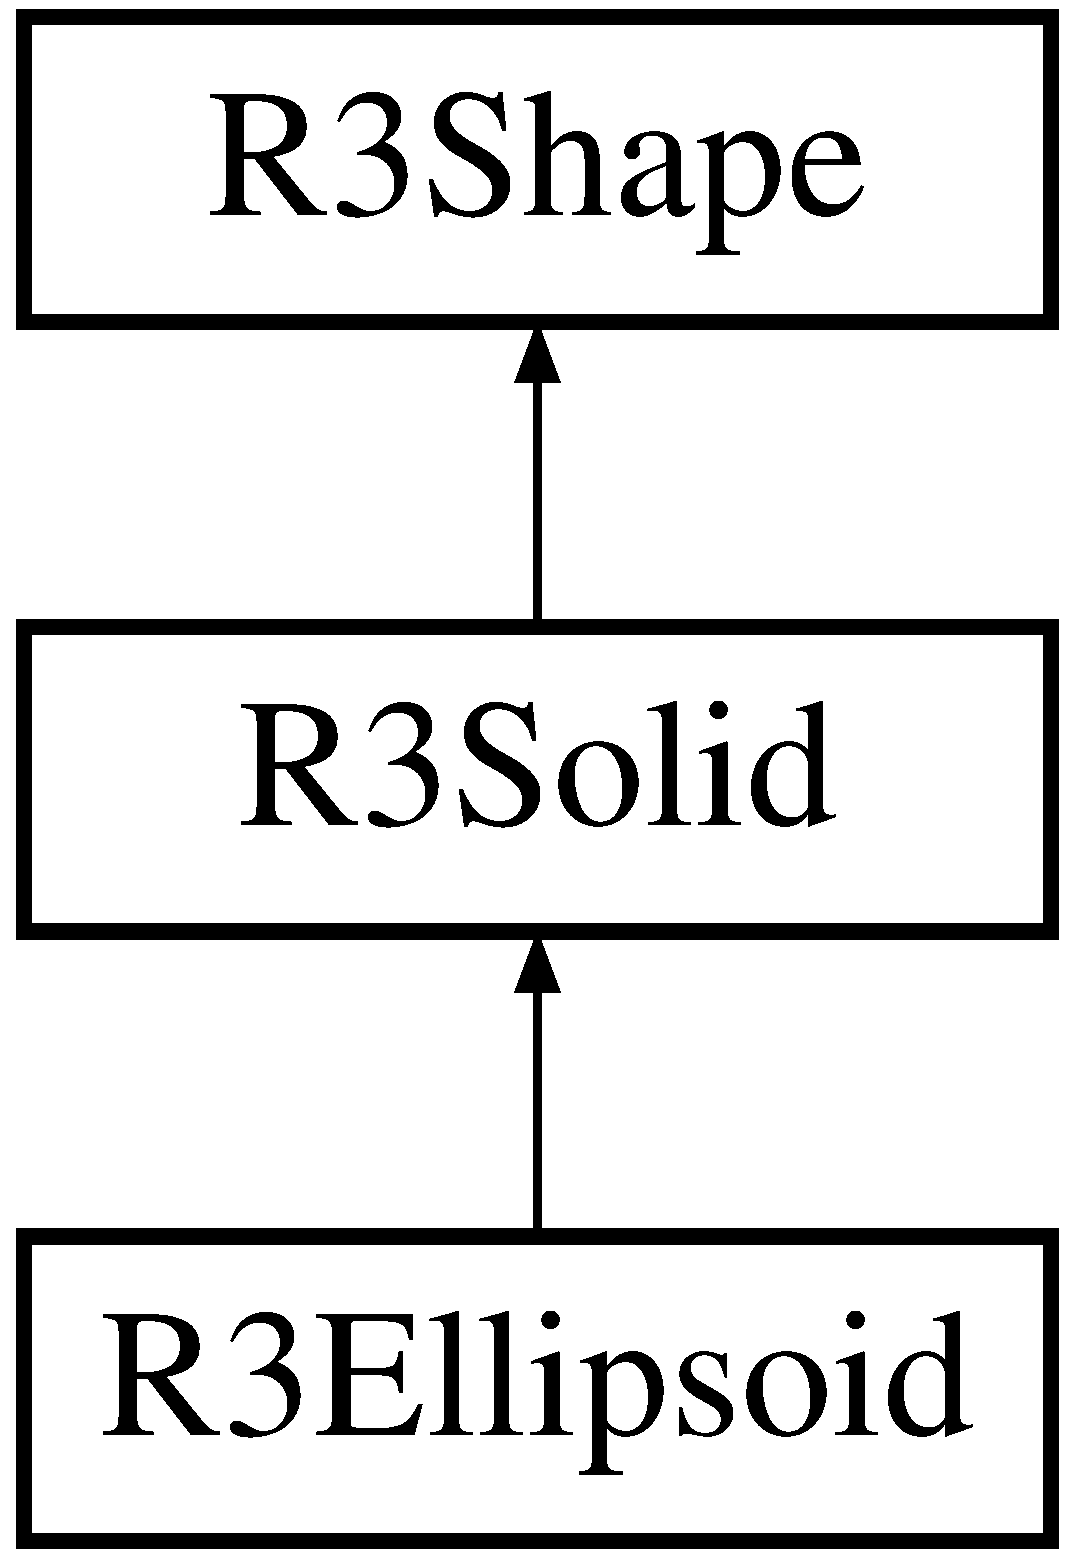
\includegraphics[height=3.000000cm]{class_r3_ellipsoid}
\end{center}
\end{figure}
\subsection*{Public Member Functions}
\begin{DoxyCompactItemize}
\item 
{\bfseries R3\+Ellipsoid} (const \hyperlink{class_r3_ellipsoid}{R3\+Ellipsoid} \&ellipsoid)\hypertarget{class_r3_ellipsoid_a01380b11c8b169200fa5854bad7b7325}{}\label{class_r3_ellipsoid_a01380b11c8b169200fa5854bad7b7325}

\item 
{\bfseries R3\+Ellipsoid} (const \hyperlink{class_r3_coord_system}{R3\+Coord\+System} \&cs, const \hyperlink{class_r3_vector}{R3\+Vector} \&radii)\hypertarget{class_r3_ellipsoid_aff8689fa86360cdd163175c62cd135d0}{}\label{class_r3_ellipsoid_aff8689fa86360cdd163175c62cd135d0}

\item 
const \hyperlink{class_r3_point}{R3\+Point} \& {\bfseries Center} (void) const \hypertarget{class_r3_ellipsoid_abf5a12db6b2ecb59462c061452bd37b5}{}\label{class_r3_ellipsoid_abf5a12db6b2ecb59462c061452bd37b5}

\item 
const \hyperlink{class_r3_coord_system}{R3\+Coord\+System} \& {\bfseries Coord\+System} (void) const \hypertarget{class_r3_ellipsoid_a2d08d79c2d5cf13a8ffd9e06f0409213}{}\label{class_r3_ellipsoid_a2d08d79c2d5cf13a8ffd9e06f0409213}

\item 
const \hyperlink{class_r3_vector}{R3\+Vector} \& {\bfseries Radii} (void) const \hypertarget{class_r3_ellipsoid_a5357d408f807072f9d978d96640aae16}{}\label{class_r3_ellipsoid_a5357d408f807072f9d978d96640aae16}

\item 
const R\+N\+Boolean {\bfseries Is\+Empty} (void) const \hypertarget{class_r3_ellipsoid_aeea13864a16cad209cd7685777b68183}{}\label{class_r3_ellipsoid_aeea13864a16cad209cd7685777b68183}

\item 
const R\+N\+Boolean {\bfseries Is\+Finite} (void) const \hypertarget{class_r3_ellipsoid_a8b141c8a15338c376a15a7864f141864}{}\label{class_r3_ellipsoid_a8b141c8a15338c376a15a7864f141864}

\item 
virtual const R\+N\+Boolean {\bfseries Is\+Point} (void) const \hypertarget{class_r3_ellipsoid_a4d024f0e86b7eb3ec7a8c7c6aba8c50c}{}\label{class_r3_ellipsoid_a4d024f0e86b7eb3ec7a8c7c6aba8c50c}

\item 
virtual const R\+N\+Boolean {\bfseries Is\+Linear} (void) const \hypertarget{class_r3_ellipsoid_ad4b9780043d72239f37bd036810665a3}{}\label{class_r3_ellipsoid_ad4b9780043d72239f37bd036810665a3}

\item 
virtual const R\+N\+Boolean {\bfseries Is\+Planar} (void) const \hypertarget{class_r3_ellipsoid_ab1ba996d9eb401d155352ff7b01b1282}{}\label{class_r3_ellipsoid_ab1ba996d9eb401d155352ff7b01b1282}

\item 
virtual const R\+N\+Boolean {\bfseries Is\+Convex} (void) const \hypertarget{class_r3_ellipsoid_aab749af98d63aa6ffe3d434e59f8324a}{}\label{class_r3_ellipsoid_aab749af98d63aa6ffe3d434e59f8324a}

\item 
virtual const \hyperlink{class_r_n_interval}{R\+N\+Interval} {\bfseries N\+Facets} (void) const \hypertarget{class_r3_ellipsoid_ace927aacc78c97175c737d3e70e26081}{}\label{class_r3_ellipsoid_ace927aacc78c97175c737d3e70e26081}

\item 
virtual const R\+N\+Area {\bfseries Area} (void) const \hypertarget{class_r3_ellipsoid_a821e4647119a978c6b582cb38317e7c4}{}\label{class_r3_ellipsoid_a821e4647119a978c6b582cb38317e7c4}

\item 
virtual const R\+N\+Volume {\bfseries Volume} (void) const \hypertarget{class_r3_ellipsoid_a9472be5a3f0d47105eb13bcb32d1f457}{}\label{class_r3_ellipsoid_a9472be5a3f0d47105eb13bcb32d1f457}

\item 
virtual const \hyperlink{class_r3_point}{R3\+Point} {\bfseries Centroid} (void) const \hypertarget{class_r3_ellipsoid_a01f50fa6d0942a7d97b41f30a1a65a3e}{}\label{class_r3_ellipsoid_a01f50fa6d0942a7d97b41f30a1a65a3e}

\item 
virtual const \hyperlink{class_r3_shape}{R3\+Shape} \& {\bfseries B\+Shape} (void) const \hypertarget{class_r3_ellipsoid_ae0aa63239317a513c83a50a44b38dd80}{}\label{class_r3_ellipsoid_ae0aa63239317a513c83a50a44b38dd80}

\item 
virtual const \hyperlink{class_r3_box}{R3\+Box} {\bfseries B\+Box} (void) const \hypertarget{class_r3_ellipsoid_a54061aeb7a37fb6617750b5898236ca3}{}\label{class_r3_ellipsoid_a54061aeb7a37fb6617750b5898236ca3}

\item 
virtual const \hyperlink{class_r3_sphere}{R3\+Sphere} {\bfseries B\+Sphere} (void) const \hypertarget{class_r3_ellipsoid_aa057f5eddb314f8d2b984197b321ce79}{}\label{class_r3_ellipsoid_aa057f5eddb314f8d2b984197b321ce79}

\item 
virtual void {\bfseries Empty} (void)\hypertarget{class_r3_ellipsoid_af935e5f553b8497248d2cab2003adc65}{}\label{class_r3_ellipsoid_af935e5f553b8497248d2cab2003adc65}

\item 
virtual void {\bfseries Translate} (const \hyperlink{class_r3_vector}{R3\+Vector} \&vector)\hypertarget{class_r3_ellipsoid_a17c49774d7dd5412c21a8a332ec65c3a}{}\label{class_r3_ellipsoid_a17c49774d7dd5412c21a8a332ec65c3a}

\item 
virtual void {\bfseries Reposition} (const \hyperlink{class_r3_point}{R3\+Point} \&center)\hypertarget{class_r3_ellipsoid_a5ee1cf7baf9453f24c92f87bfc576e69}{}\label{class_r3_ellipsoid_a5ee1cf7baf9453f24c92f87bfc576e69}

\item 
virtual void {\bfseries Resize} (const \hyperlink{class_r3_vector}{R3\+Vector} \&radii)\hypertarget{class_r3_ellipsoid_a92f5f138077637b9fa5552c8c0ae76a4}{}\label{class_r3_ellipsoid_a92f5f138077637b9fa5552c8c0ae76a4}

\item 
virtual void {\bfseries Transform} (const \hyperlink{class_r3_transformation}{R3\+Transformation} \&transformation)\hypertarget{class_r3_ellipsoid_ad05892338bcb2b7c032d9aa8ab9ea89a}{}\label{class_r3_ellipsoid_ad05892338bcb2b7c032d9aa8ab9ea89a}

\item 
virtual void {\bfseries Draw} (const \hyperlink{class_r_n_flags}{R3\+Draw\+Flags} draw\+\_\+flags=R3\+\_\+\+D\+E\+F\+A\+U\+L\+T\+\_\+\+D\+R\+A\+W\+\_\+\+F\+L\+A\+GS) const \hypertarget{class_r3_ellipsoid_a8ba33ceec3fcfc4147190daff77e9c26}{}\label{class_r3_ellipsoid_a8ba33ceec3fcfc4147190daff77e9c26}

\item 
R\+N\+Boolean {\bfseries operator==} (const \hyperlink{class_r3_ellipsoid}{R3\+Ellipsoid} \&ellipsoid) const \hypertarget{class_r3_ellipsoid_a5f1a75a4f115295cae03cd4ae8db314b}{}\label{class_r3_ellipsoid_a5f1a75a4f115295cae03cd4ae8db314b}

\item 
R\+N\+Boolean {\bfseries operator!=} (const \hyperlink{class_r3_ellipsoid}{R3\+Ellipsoid} \&ellipsoid) const \hypertarget{class_r3_ellipsoid_a9c250b4b6ea88ff48b5b2eb9eb213c02}{}\label{class_r3_ellipsoid_a9c250b4b6ea88ff48b5b2eb9eb213c02}

\item 
{\bfseries R\+N\+\_\+\+C\+L\+A\+S\+S\+\_\+\+T\+Y\+P\+E\+\_\+\+D\+E\+C\+L\+A\+R\+A\+T\+I\+O\+NS} (\hyperlink{class_r3_ellipsoid}{R3\+Ellipsoid})\hypertarget{class_r3_ellipsoid_ac1b6ac4e5624791735c4519c865eaf48}{}\label{class_r3_ellipsoid_ac1b6ac4e5624791735c4519c865eaf48}

\item 
{\bfseries R3\+\_\+\+S\+H\+A\+P\+E\+\_\+\+R\+E\+L\+A\+T\+I\+O\+N\+S\+H\+I\+P\+\_\+\+D\+E\+C\+L\+A\+R\+A\+T\+I\+O\+NS} (\hyperlink{class_r3_ellipsoid}{R3\+Ellipsoid})\hypertarget{class_r3_ellipsoid_a0998386a1093e03bd9826a0eee8d6f6d}{}\label{class_r3_ellipsoid_a0998386a1093e03bd9826a0eee8d6f6d}

\item 
void {\bfseries Update\+B\+Box} (void)\hypertarget{class_r3_ellipsoid_abd9dffc092074e55c3d2d0d8620cc381}{}\label{class_r3_ellipsoid_abd9dffc092074e55c3d2d0d8620cc381}

\end{DoxyCompactItemize}


The documentation for this class was generated from the following files\+:\begin{DoxyCompactItemize}
\item 
R3\+Shapes/R3\+Ellipsoid.\+h\item 
R3\+Shapes/R3\+Draw.\+cpp\item 
R3\+Shapes/R3\+Ellipsoid.\+cpp\end{DoxyCompactItemize}

\hypertarget{struct_r3_frustum}{}\section{R3\+Frustum Struct Reference}
\label{struct_r3_frustum}\index{R3\+Frustum@{R3\+Frustum}}
\subsection*{Public Member Functions}
\begin{DoxyCompactItemize}
\item 
{\bfseries R3\+Frustum} (const \hyperlink{class_r3_camera}{R3\+Camera} \&camera)\hypertarget{struct_r3_frustum_ad2560ce0693fe855cfe601ed00651701}{}\label{struct_r3_frustum_ad2560ce0693fe855cfe601ed00651701}

\item 
{\bfseries R3\+Frustum} (const \hyperlink{class_r3_point}{R3\+Point} \&viewpoint, const \hyperlink{class_r3_vector}{R3\+Vector} \&towards, const \hyperlink{class_r3_vector}{R3\+Vector} \&up, R\+N\+Angle xfov, R\+N\+Angle yfov, R\+N\+Length neardist, R\+N\+Length fardist)\hypertarget{struct_r3_frustum_aab15ed12f3aef3028427d1cf685c5b23}{}\label{struct_r3_frustum_aab15ed12f3aef3028427d1cf685c5b23}

\item 
const \hyperlink{class_r3_camera}{R3\+Camera} \& {\bfseries Camera} (void) const \hypertarget{struct_r3_frustum_a7a92ddc7b16b5ecf9ed0ca7972d27320}{}\label{struct_r3_frustum_a7a92ddc7b16b5ecf9ed0ca7972d27320}

\item 
const \hyperlink{class_r3_halfspace}{R3\+Halfspace} \& {\bfseries Halfspace} (int dir, int dim) const \hypertarget{struct_r3_frustum_a8383513c86ed5dc77c6ef446db2ddf75}{}\label{struct_r3_frustum_a8383513c86ed5dc77c6ef446db2ddf75}

\item 
void {\bfseries Set\+Camera} (const \hyperlink{class_r3_camera}{R3\+Camera} \&camera)\hypertarget{struct_r3_frustum_a5f950afb6109bf79fd41174844fd6fcb}{}\label{struct_r3_frustum_a5f950afb6109bf79fd41174844fd6fcb}

\item 
R\+N\+Boolean {\bfseries Intersects} (const \hyperlink{class_r3_point}{R3\+Point} \&point) const \hypertarget{struct_r3_frustum_a3ba00858b6906f6b4b5aa17a6307f32d}{}\label{struct_r3_frustum_a3ba00858b6906f6b4b5aa17a6307f32d}

\item 
R\+N\+Boolean {\bfseries Intersects} (const \hyperlink{class_r3_span}{R3\+Span} \&span) const \hypertarget{struct_r3_frustum_a706e0b3936b5f8c59001f101b11531c2}{}\label{struct_r3_frustum_a706e0b3936b5f8c59001f101b11531c2}

\item 
R\+N\+Boolean {\bfseries Intersects} (const \hyperlink{class_r3_box}{R3\+Box} \&\hyperlink{structbox}{box}) const \hypertarget{struct_r3_frustum_a0ac494f2de905ce5644bb5ffadf8099b}{}\label{struct_r3_frustum_a0ac494f2de905ce5644bb5ffadf8099b}

\item 
R\+N\+Boolean {\bfseries Contains} (const \hyperlink{class_r3_point}{R3\+Point} \&point) const \hypertarget{struct_r3_frustum_a5c8e2c1824f9a9312adbdc936f70d920}{}\label{struct_r3_frustum_a5c8e2c1824f9a9312adbdc936f70d920}

\item 
R\+N\+Boolean {\bfseries Contains} (const \hyperlink{class_r3_span}{R3\+Span} \&span) const \hypertarget{struct_r3_frustum_a7b5430be3f72ec0cb75295788f33357b}{}\label{struct_r3_frustum_a7b5430be3f72ec0cb75295788f33357b}

\item 
R\+N\+Boolean {\bfseries Contains} (const \hyperlink{class_r3_box}{R3\+Box} \&\hyperlink{structbox}{box}) const \hypertarget{struct_r3_frustum_a9462950da6a7bccacad9145aeba864d0}{}\label{struct_r3_frustum_a9462950da6a7bccacad9145aeba864d0}

\item 
void {\bfseries Draw} (void) const \hypertarget{struct_r3_frustum_a28b625c7c0975f8261b2604cd174c02a}{}\label{struct_r3_frustum_a28b625c7c0975f8261b2604cd174c02a}

\end{DoxyCompactItemize}
\subsection*{Public Attributes}
\begin{DoxyCompactItemize}
\item 
\hyperlink{class_r3_camera}{R3\+Camera} {\bfseries camera}\hypertarget{struct_r3_frustum_a01976de96489f9aa190b5512aaa58964}{}\label{struct_r3_frustum_a01976de96489f9aa190b5512aaa58964}

\item 
\hyperlink{class_r3_halfspace}{R3\+Halfspace} {\bfseries halfspaces} \mbox{[}2\mbox{]}\mbox{[}3\mbox{]}\hypertarget{struct_r3_frustum_a1fbff48418da119afd0f35dfdce5419f}{}\label{struct_r3_frustum_a1fbff48418da119afd0f35dfdce5419f}

\end{DoxyCompactItemize}


The documentation for this struct was generated from the following files\+:\begin{DoxyCompactItemize}
\item 
R3\+Graphics/R3\+Frustum.\+h\item 
R3\+Graphics/R3\+Frustum.\+cpp\end{DoxyCompactItemize}

\hypertarget{class_r3_grid}{}\section{R3\+Grid Class Reference}
\label{class_r3_grid}\index{R3\+Grid@{R3\+Grid}}
\subsection*{Public Member Functions}
\begin{DoxyCompactItemize}
\item 
{\bfseries R3\+Grid} (int xresolution=0, int yresolution=0, int zresolution=0)\hypertarget{class_r3_grid_a263b696638a1862f4bd0c58b41acd348}{}\label{class_r3_grid_a263b696638a1862f4bd0c58b41acd348}

\item 
{\bfseries R3\+Grid} (int xresolution, int yresolution, int zresolution, const \hyperlink{class_r3_box}{R3\+Box} \&bbox)\hypertarget{class_r3_grid_a45805d701919185e394bad166f5a3819}{}\label{class_r3_grid_a45805d701919185e394bad166f5a3819}

\item 
{\bfseries R3\+Grid} (const \hyperlink{class_r3_grid}{R3\+Grid} \&grid)\hypertarget{class_r3_grid_a50260941a5e1fa98f4bf97fc5eb7ca81}{}\label{class_r3_grid_a50260941a5e1fa98f4bf97fc5eb7ca81}

\item 
int {\bfseries N\+Entries} (void) const \hypertarget{class_r3_grid_a660610b234dd833dcd77e42ec2dab6d2}{}\label{class_r3_grid_a660610b234dd833dcd77e42ec2dab6d2}

\item 
int {\bfseries X\+Resolution} (void) const \hypertarget{class_r3_grid_ab78e0abfd74d78ba3588ab213ef77b93}{}\label{class_r3_grid_ab78e0abfd74d78ba3588ab213ef77b93}

\item 
int {\bfseries Y\+Resolution} (void) const \hypertarget{class_r3_grid_a15520d5de7cc5bdfc598fd49c0a14da9}{}\label{class_r3_grid_a15520d5de7cc5bdfc598fd49c0a14da9}

\item 
int {\bfseries Z\+Resolution} (void) const \hypertarget{class_r3_grid_a71e26a27a5a211d9c6bf15534f10234a}{}\label{class_r3_grid_a71e26a27a5a211d9c6bf15534f10234a}

\item 
int {\bfseries Resolution} (R\+N\+Dimension dim) const \hypertarget{class_r3_grid_a0d2f24715ad10008e18b303471237c44}{}\label{class_r3_grid_a0d2f24715ad10008e18b303471237c44}

\item 
R\+N\+Scalar {\bfseries Sum} (void) const \hypertarget{class_r3_grid_a442881ed78cd7529ec2553e962bbee32}{}\label{class_r3_grid_a442881ed78cd7529ec2553e962bbee32}

\item 
R\+N\+Scalar {\bfseries Mean} (void) const \hypertarget{class_r3_grid_a94d5131f557c70b1eddb9f3027e1f1d1}{}\label{class_r3_grid_a94d5131f557c70b1eddb9f3027e1f1d1}

\item 
R\+N\+Scalar {\bfseries Variance} (void) const \hypertarget{class_r3_grid_a2f1d640bcc02f0b69568751e5fc6129c}{}\label{class_r3_grid_a2f1d640bcc02f0b69568751e5fc6129c}

\item 
R\+N\+Scalar {\bfseries Standard\+Deviation} (void) const \hypertarget{class_r3_grid_aeb1547eb08ba34eabe10c91c88f8db19}{}\label{class_r3_grid_aeb1547eb08ba34eabe10c91c88f8db19}

\item 
R\+N\+Scalar {\bfseries Maximum} (void) const \hypertarget{class_r3_grid_ab1c3855abd356d4f859783b270e2c18d}{}\label{class_r3_grid_ab1c3855abd356d4f859783b270e2c18d}

\item 
R\+N\+Scalar {\bfseries Minimum} (void) const \hypertarget{class_r3_grid_a57b0b540031dec0c0b0667388802d421}{}\label{class_r3_grid_a57b0b540031dec0c0b0667388802d421}

\item 
\hyperlink{class_r_n_interval}{R\+N\+Interval} {\bfseries Range} (void) const \hypertarget{class_r3_grid_a16dada6237aa354105da865ceed91309}{}\label{class_r3_grid_a16dada6237aa354105da865ceed91309}

\item 
R\+N\+Scalar {\bfseries L1\+Norm} (void) const \hypertarget{class_r3_grid_a9d75fff6eaa62e629d409cec822abfa7}{}\label{class_r3_grid_a9d75fff6eaa62e629d409cec822abfa7}

\item 
R\+N\+Scalar {\bfseries L2\+Norm} (void) const \hypertarget{class_r3_grid_a60ad29ae5b8c7cca534a788ef9219fa5}{}\label{class_r3_grid_a60ad29ae5b8c7cca534a788ef9219fa5}

\item 
R\+N\+Scalar {\bfseries L2\+Norm\+Squared} (void) const \hypertarget{class_r3_grid_a0dc299cf0083e9e3de6bf8676ee5694e}{}\label{class_r3_grid_a0dc299cf0083e9e3de6bf8676ee5694e}

\item 
R\+N\+Scalar {\bfseries Volume} (void) const \hypertarget{class_r3_grid_a1335f955ca44933b61f2df596bdabad7}{}\label{class_r3_grid_a1335f955ca44933b61f2df596bdabad7}

\item 
int {\bfseries Cardinality} (void) const \hypertarget{class_r3_grid_a43b6b6ea920d3682fc6d8976722b2b86}{}\label{class_r3_grid_a43b6b6ea920d3682fc6d8976722b2b86}

\item 
\hyperlink{class_r3_box}{R3\+Box} {\bfseries Grid\+Box} (void) const \hypertarget{class_r3_grid_a0220bb241e1811504e791489fe190d94}{}\label{class_r3_grid_a0220bb241e1811504e791489fe190d94}

\item 
\hyperlink{class_r3_box}{R3\+Box} {\bfseries World\+Box} (void) const \hypertarget{class_r3_grid_ad4c53c72856d85f39528bb2afefc93ad}{}\label{class_r3_grid_ad4c53c72856d85f39528bb2afefc93ad}

\item 
\hyperlink{class_r3_point}{R3\+Point} {\bfseries Grid\+Centroid} (void) const \hypertarget{class_r3_grid_a498251035c00a76d170cd8175315706a}{}\label{class_r3_grid_a498251035c00a76d170cd8175315706a}

\item 
\hyperlink{class_r3_point}{R3\+Point} {\bfseries World\+Centroid} (void) const \hypertarget{class_r3_grid_ab6649e77922981d56bafe73d14eec15d}{}\label{class_r3_grid_ab6649e77922981d56bafe73d14eec15d}

\item 
\hyperlink{class_r3_triad}{R3\+Triad} {\bfseries Grid\+Principle\+Axes} (const \hyperlink{class_r3_point}{R3\+Point} $\ast$grid\+\_\+centroid=N\+U\+LL, R\+N\+Scalar $\ast$variances=N\+U\+LL) const \hypertarget{class_r3_grid_a67fa61029dd8c50daa9685e921af1466}{}\label{class_r3_grid_a67fa61029dd8c50daa9685e921af1466}

\item 
\hyperlink{class_r3_triad}{R3\+Triad} {\bfseries World\+Principle\+Axes} (const \hyperlink{class_r3_point}{R3\+Point} $\ast$world\+\_\+centroid=N\+U\+LL, R\+N\+Scalar $\ast$variances=N\+U\+LL) const \hypertarget{class_r3_grid_ad35c0896a09ee3df94469ea767a460af}{}\label{class_r3_grid_ad35c0896a09ee3df94469ea767a460af}

\item 
\hyperlink{class_r2_grid}{R2\+Grid} $\ast$ {\bfseries Slice} (int dim, int grid\+\_\+coordinate) const \hypertarget{class_r3_grid_af0fb6fc03c4a8ab08b91ec83eb4ed163}{}\label{class_r3_grid_af0fb6fc03c4a8ab08b91ec83eb4ed163}

\item 
const \hyperlink{class_r3_affine}{R3\+Affine} \& {\bfseries World\+To\+Grid\+Transformation} (void) const \hypertarget{class_r3_grid_a517ac6a77a7e3f3dc7d9e740a4a301fb}{}\label{class_r3_grid_a517ac6a77a7e3f3dc7d9e740a4a301fb}

\item 
const \hyperlink{class_r3_affine}{R3\+Affine} \& {\bfseries Grid\+To\+World\+Transformation} (void) const \hypertarget{class_r3_grid_a98e58af13264ef62cf73d65b0345eed0}{}\label{class_r3_grid_a98e58af13264ef62cf73d65b0345eed0}

\item 
R\+N\+Scalar {\bfseries World\+To\+Grid\+Scale\+Factor} (void) const \hypertarget{class_r3_grid_a4ddc8f0e71d6c7b91174fd13f79055da}{}\label{class_r3_grid_a4ddc8f0e71d6c7b91174fd13f79055da}

\item 
R\+N\+Scalar {\bfseries Grid\+To\+World\+Scale\+Factor} (void) const \hypertarget{class_r3_grid_a3bcab7a9c9454140671c182b5810b511}{}\label{class_r3_grid_a3bcab7a9c9454140671c182b5810b511}

\item 
R\+N\+Scalar {\bfseries World\+Spacing} (R\+N\+Dimension dim) const \hypertarget{class_r3_grid_ac29850cd40934389397170219d44e7ea}{}\label{class_r3_grid_ac29850cd40934389397170219d44e7ea}

\item 
R\+N\+Scalar {\bfseries Grid\+Value} (int index) const \hypertarget{class_r3_grid_a871c36cc7fe6f9de2a4cd479d2075933}{}\label{class_r3_grid_a871c36cc7fe6f9de2a4cd479d2075933}

\item 
R\+N\+Scalar {\bfseries Grid\+Value} (int i, int j, int k) const \hypertarget{class_r3_grid_a2e80c4ba576665d55ac044b29be5b375}{}\label{class_r3_grid_a2e80c4ba576665d55ac044b29be5b375}

\item 
R\+N\+Scalar {\bfseries Grid\+Value} (R\+N\+Coord x, R\+N\+Coord y, R\+N\+Coord z) const \hypertarget{class_r3_grid_ac1eaa2fcbea166a3e62875531858278c}{}\label{class_r3_grid_ac1eaa2fcbea166a3e62875531858278c}

\item 
R\+N\+Scalar {\bfseries Grid\+Value} (const \hyperlink{class_r3_point}{R3\+Point} \&grid\+\_\+point) const \hypertarget{class_r3_grid_a0c55f4fac41aa4e80737f1255afb185c}{}\label{class_r3_grid_a0c55f4fac41aa4e80737f1255afb185c}

\item 
R\+N\+Scalar {\bfseries World\+Value} (R\+N\+Coord x, R\+N\+Coord y, R\+N\+Coord z) const \hypertarget{class_r3_grid_a0af5826aceb1f4ceb97469015dfc51fd}{}\label{class_r3_grid_a0af5826aceb1f4ceb97469015dfc51fd}

\item 
R\+N\+Scalar {\bfseries World\+Value} (const \hyperlink{class_r3_point}{R3\+Point} \&world\+\_\+point) const \hypertarget{class_r3_grid_a0729fc2c709c4f51192099990b2f41ac}{}\label{class_r3_grid_a0729fc2c709c4f51192099990b2f41ac}

\item 
R\+N\+Scalar \& {\bfseries operator()} (int i, int j, int k)\hypertarget{class_r3_grid_acd5c37f10c4a9030c87c134c1c2e35bf}{}\label{class_r3_grid_acd5c37f10c4a9030c87c134c1c2e35bf}

\item 
void {\bfseries Abs} (void)\hypertarget{class_r3_grid_a39a47b010ee0a1010ae44b5509021f9e}{}\label{class_r3_grid_a39a47b010ee0a1010ae44b5509021f9e}

\item 
void {\bfseries Sqrt} (void)\hypertarget{class_r3_grid_afec9b5b5bfff61f34c0c63adf94d5e87}{}\label{class_r3_grid_afec9b5b5bfff61f34c0c63adf94d5e87}

\item 
void {\bfseries Square} (void)\hypertarget{class_r3_grid_aadef1b026fd93b3f23ec5f12e5a621b0}{}\label{class_r3_grid_aadef1b026fd93b3f23ec5f12e5a621b0}

\item 
void {\bfseries Negate} (void)\hypertarget{class_r3_grid_a2275b93c175ddd0678b5232fc4ad508a}{}\label{class_r3_grid_a2275b93c175ddd0678b5232fc4ad508a}

\item 
void {\bfseries Invert} (void)\hypertarget{class_r3_grid_a716a008023b16f52ed84567435bc4466}{}\label{class_r3_grid_a716a008023b16f52ed84567435bc4466}

\item 
void {\bfseries Transpose} (void)\hypertarget{class_r3_grid_ac073242feee587be9b481313be88c0f7}{}\label{class_r3_grid_ac073242feee587be9b481313be88c0f7}

\item 
void {\bfseries Normalize} (void)\hypertarget{class_r3_grid_a7445ecffaa255533fd8a6f0f214dab84}{}\label{class_r3_grid_a7445ecffaa255533fd8a6f0f214dab84}

\item 
void {\bfseries Convolve} (const R\+N\+Scalar filter\mbox{[}3\mbox{]}\mbox{[}3\mbox{]}\mbox{[}3\mbox{]})\hypertarget{class_r3_grid_a2c092da25929f56e0f751267d4d89b79}{}\label{class_r3_grid_a2c092da25929f56e0f751267d4d89b79}

\item 
void {\bfseries Laplacian} (void)\hypertarget{class_r3_grid_aee8f2a41426d97be49bca26b6e9300c6}{}\label{class_r3_grid_aee8f2a41426d97be49bca26b6e9300c6}

\item 
void {\bfseries Gradient} (R\+N\+Dimension dim)\hypertarget{class_r3_grid_a16295f56ac5bd7c8b7b40c01876e62ca}{}\label{class_r3_grid_a16295f56ac5bd7c8b7b40c01876e62ca}

\item 
void {\bfseries Gradient\+Magnitude} (void)\hypertarget{class_r3_grid_ac3e7a5b7c4e57a3df01e0b3df49c1ae5}{}\label{class_r3_grid_ac3e7a5b7c4e57a3df01e0b3df49c1ae5}

\item 
void {\bfseries Detect\+Edges} (void)\hypertarget{class_r3_grid_ac28e72ecc029f51ba86351f652d388b7}{}\label{class_r3_grid_ac28e72ecc029f51ba86351f652d388b7}

\item 
void {\bfseries Dilate} (R\+N\+Scalar grid\+\_\+distance)\hypertarget{class_r3_grid_a8adc3216f57c35fca6cc334658222073}{}\label{class_r3_grid_a8adc3216f57c35fca6cc334658222073}

\item 
void {\bfseries Erode} (R\+N\+Scalar grid\+\_\+distance)\hypertarget{class_r3_grid_a053615b5dfd296d03de9d3342a5bd69b}{}\label{class_r3_grid_a053615b5dfd296d03de9d3342a5bd69b}

\item 
void {\bfseries Blur} (R\+N\+Scalar grid\+\_\+sigma=2)\hypertarget{class_r3_grid_a173ed5e2e752422fd12fc560fe0d8d70}{}\label{class_r3_grid_a173ed5e2e752422fd12fc560fe0d8d70}

\item 
void {\bfseries Bilateral\+Filter} (R\+N\+Length grid\+\_\+sigma=2, R\+N\+Scalar value\+\_\+sigma=-\/1)\hypertarget{class_r3_grid_a1316c3649f21bd00e1ca016ce1ce1caf}{}\label{class_r3_grid_a1316c3649f21bd00e1ca016ce1ce1caf}

\item 
void {\bfseries Percentile\+Filter} (R\+N\+Length grid\+\_\+radius, R\+N\+Scalar percentile)\hypertarget{class_r3_grid_a511d9bb2e6eaa42c9c0e917009da90b1}{}\label{class_r3_grid_a511d9bb2e6eaa42c9c0e917009da90b1}

\item 
void {\bfseries Min\+Filter} (R\+N\+Length grid\+\_\+radius)\hypertarget{class_r3_grid_aa2b97236e2b43359023f47634ac098fe}{}\label{class_r3_grid_aa2b97236e2b43359023f47634ac098fe}

\item 
void {\bfseries Max\+Filter} (R\+N\+Length grid\+\_\+radius)\hypertarget{class_r3_grid_ac54562bc053bbfde118e58f2411b089a}{}\label{class_r3_grid_ac54562bc053bbfde118e58f2411b089a}

\item 
void {\bfseries Median\+Filter} (R\+N\+Length grid\+\_\+radius)\hypertarget{class_r3_grid_a7e88ed91dc5c72b0ee9b62966c29715d}{}\label{class_r3_grid_a7e88ed91dc5c72b0ee9b62966c29715d}

\item 
void {\bfseries Mask\+Non\+Minima} (R\+N\+Length grid\+\_\+radius=0)\hypertarget{class_r3_grid_a15468c7af24ce6496956a03be1b4d0b8}{}\label{class_r3_grid_a15468c7af24ce6496956a03be1b4d0b8}

\item 
void {\bfseries Mask\+Non\+Maxima} (R\+N\+Length grid\+\_\+radius=0)\hypertarget{class_r3_grid_a10f0a4cd8c16f11facaa817e6a30a81a}{}\label{class_r3_grid_a10f0a4cd8c16f11facaa817e6a30a81a}

\item 
void {\bfseries Clear} (R\+N\+Scalar value=0)\hypertarget{class_r3_grid_a9221437f915eeb8fb73a6a06fe219545}{}\label{class_r3_grid_a9221437f915eeb8fb73a6a06fe219545}

\item 
void {\bfseries Substitute} (R\+N\+Scalar old\+\_\+value, R\+N\+Scalar new\+\_\+value)\hypertarget{class_r3_grid_a843bc03547c84f65b7349a4ea2ce1439}{}\label{class_r3_grid_a843bc03547c84f65b7349a4ea2ce1439}

\item 
void {\bfseries Add} (R\+N\+Scalar value)\hypertarget{class_r3_grid_a3d366202bec97966afd7f43dbb303ac4}{}\label{class_r3_grid_a3d366202bec97966afd7f43dbb303ac4}

\item 
void {\bfseries Copy} (const \hyperlink{class_r3_grid}{R3\+Grid} \&grid)\hypertarget{class_r3_grid_a5b9f1c37fdb1037bde88a032f5f1675a}{}\label{class_r3_grid_a5b9f1c37fdb1037bde88a032f5f1675a}

\item 
void {\bfseries Add} (const \hyperlink{class_r3_grid}{R3\+Grid} \&grid)\hypertarget{class_r3_grid_aae66b9b898621a40f6823b9965b778ce}{}\label{class_r3_grid_aae66b9b898621a40f6823b9965b778ce}

\item 
void {\bfseries Add} (const \hyperlink{class_r3_grid}{R3\+Grid} \&grid, const \hyperlink{class_r3_point}{R3\+Point} \&grid\+\_\+position, const \hyperlink{class_r3_point}{R3\+Point} \&filter\+\_\+origin, R\+N\+Scalar amplitude=1)\hypertarget{class_r3_grid_a7d39171de5aca13f5a59c8cf8246cf9e}{}\label{class_r3_grid_a7d39171de5aca13f5a59c8cf8246cf9e}

\item 
void {\bfseries Subtract} (R\+N\+Scalar value)\hypertarget{class_r3_grid_aea6fd52af1ab0e4a2ae878f8d7123141}{}\label{class_r3_grid_aea6fd52af1ab0e4a2ae878f8d7123141}

\item 
void {\bfseries Subtract} (const \hyperlink{class_r3_grid}{R3\+Grid} \&grid)\hypertarget{class_r3_grid_a21012076c66a167c5b794a8a996d0f9b}{}\label{class_r3_grid_a21012076c66a167c5b794a8a996d0f9b}

\item 
void {\bfseries Multiply} (R\+N\+Scalar value)\hypertarget{class_r3_grid_a17cbcc2010c459c676f57431f5fd4926}{}\label{class_r3_grid_a17cbcc2010c459c676f57431f5fd4926}

\item 
void {\bfseries Multiply} (const \hyperlink{class_r3_grid}{R3\+Grid} \&grid)\hypertarget{class_r3_grid_a0551d01268fb98d7ef285c71f7dd6366}{}\label{class_r3_grid_a0551d01268fb98d7ef285c71f7dd6366}

\item 
void {\bfseries Divide} (R\+N\+Scalar value)\hypertarget{class_r3_grid_aa667c0b95037da317574afe473516eba}{}\label{class_r3_grid_aa667c0b95037da317574afe473516eba}

\item 
void {\bfseries Divide} (const \hyperlink{class_r3_grid}{R3\+Grid} \&grid)\hypertarget{class_r3_grid_a498e21a749229027ea781404a026d1f4}{}\label{class_r3_grid_a498e21a749229027ea781404a026d1f4}

\item 
void {\bfseries Pow} (R\+N\+Scalar exponent)\hypertarget{class_r3_grid_a4920beffa01692f1d4c2c97d1bfc44d4}{}\label{class_r3_grid_a4920beffa01692f1d4c2c97d1bfc44d4}

\item 
void {\bfseries Mask} (const \hyperlink{class_r3_grid}{R3\+Grid} \&grid)\hypertarget{class_r3_grid_a15befdb60b898045b36d00c2c4057355}{}\label{class_r3_grid_a15befdb60b898045b36d00c2c4057355}

\item 
void {\bfseries Threshold} (R\+N\+Scalar threshold, R\+N\+Scalar low, R\+N\+Scalar high)\hypertarget{class_r3_grid_aadc7fd47c3efc3eb0f4183475c53258a}{}\label{class_r3_grid_aadc7fd47c3efc3eb0f4183475c53258a}

\item 
void {\bfseries Signed\+Distance\+Transform} (void)\hypertarget{class_r3_grid_ad11edc63b98ee9e456d77edf39227a08}{}\label{class_r3_grid_ad11edc63b98ee9e456d77edf39227a08}

\item 
void {\bfseries Squared\+Distance\+Transform} (void)\hypertarget{class_r3_grid_af52aaf1a7d2dbabb5d5c2fccaa9a2847}{}\label{class_r3_grid_af52aaf1a7d2dbabb5d5c2fccaa9a2847}

\item 
void {\bfseries Voronoi} (\hyperlink{class_r3_grid}{R3\+Grid} $\ast$squared\+\_\+distance\+\_\+grid=N\+U\+LL)\hypertarget{class_r3_grid_acbac4ab75e1778977192dd31f63c8a55}{}\label{class_r3_grid_acbac4ab75e1778977192dd31f63c8a55}

\item 
void {\bfseries Gauss} (R\+N\+Length sigma=sqrt(8.\+0), R\+N\+Boolean square=T\+R\+UE)\hypertarget{class_r3_grid_a810bb08b0b9f06683b0d644d6c15be46}{}\label{class_r3_grid_a810bb08b0b9f06683b0d644d6c15be46}

\item 
void {\bfseries Resample} (int xres, int yres, int zres)\hypertarget{class_r3_grid_a7b6f21015449cea493b9a6024294832d}{}\label{class_r3_grid_a7b6f21015449cea493b9a6024294832d}

\item 
void {\bfseries Pad\+With\+Zero} (int xres, int yres, int zres, int xoffset=0, int yoffset=0, int zoffset=0)\hypertarget{class_r3_grid_ac95653c58e341f4d958b6c27baf72f61}{}\label{class_r3_grid_ac95653c58e341f4d958b6c27baf72f61}

\item 
void {\bfseries Cluster\+With\+Mean\+Shift} (void)\hypertarget{class_r3_grid_a2a19534deaa0527981086939880ebba5}{}\label{class_r3_grid_a2a19534deaa0527981086939880ebba5}

\item 
void {\bfseries Set\+Grid\+Value} (int index, R\+N\+Scalar value)\hypertarget{class_r3_grid_a74e2d1b586c58448fd27004e8a121e1c}{}\label{class_r3_grid_a74e2d1b586c58448fd27004e8a121e1c}

\item 
void {\bfseries Set\+Grid\+Value} (int i, int j, int k, R\+N\+Scalar value)\hypertarget{class_r3_grid_a45e1188ab7ac8912872235076555b2d0}{}\label{class_r3_grid_a45e1188ab7ac8912872235076555b2d0}

\item 
void {\bfseries Add\+Grid\+Value} (int i, int j, int k, R\+N\+Scalar value)\hypertarget{class_r3_grid_ad99264ba45cbc7bcd2c29858341baba1}{}\label{class_r3_grid_ad99264ba45cbc7bcd2c29858341baba1}

\item 
\hyperlink{class_r3_grid}{R3\+Grid} \& {\bfseries operator=} (const \hyperlink{class_r3_grid}{R3\+Grid} \&grid)\hypertarget{class_r3_grid_a51a010d2037d0dd2c441bb389f68508b}{}\label{class_r3_grid_a51a010d2037d0dd2c441bb389f68508b}

\item 
\hyperlink{class_r3_grid}{R3\+Grid} \& {\bfseries operator+=} (R\+N\+Scalar scale)\hypertarget{class_r3_grid_a73e42fb1dbcf363cd0062a0346fff738}{}\label{class_r3_grid_a73e42fb1dbcf363cd0062a0346fff738}

\item 
\hyperlink{class_r3_grid}{R3\+Grid} \& {\bfseries operator+=} (const \hyperlink{class_r3_grid}{R3\+Grid} \&grid)\hypertarget{class_r3_grid_ae205c5b18ca6d53c71c29d10a8b7bc2c}{}\label{class_r3_grid_ae205c5b18ca6d53c71c29d10a8b7bc2c}

\item 
\hyperlink{class_r3_grid}{R3\+Grid} \& {\bfseries operator-\/=} (R\+N\+Scalar scale)\hypertarget{class_r3_grid_a4f8ea398e5f7cbf278b4277835c87660}{}\label{class_r3_grid_a4f8ea398e5f7cbf278b4277835c87660}

\item 
\hyperlink{class_r3_grid}{R3\+Grid} \& {\bfseries operator-\/=} (const \hyperlink{class_r3_grid}{R3\+Grid} \&grid)\hypertarget{class_r3_grid_ae5e799bf941da4baf6ebb263abe25408}{}\label{class_r3_grid_ae5e799bf941da4baf6ebb263abe25408}

\item 
\hyperlink{class_r3_grid}{R3\+Grid} \& {\bfseries operator$\ast$=} (R\+N\+Scalar scale)\hypertarget{class_r3_grid_a9fea1d5d839e44feaa3374efeee1013b}{}\label{class_r3_grid_a9fea1d5d839e44feaa3374efeee1013b}

\item 
\hyperlink{class_r3_grid}{R3\+Grid} \& {\bfseries operator$\ast$=} (const \hyperlink{class_r3_grid}{R3\+Grid} \&grid)\hypertarget{class_r3_grid_afe86741fec425bac6755cc4cb61cb5fc}{}\label{class_r3_grid_afe86741fec425bac6755cc4cb61cb5fc}

\item 
\hyperlink{class_r3_grid}{R3\+Grid} \& {\bfseries operator/=} (R\+N\+Scalar scale)\hypertarget{class_r3_grid_abfb6096d07f786be42384cdb7083be6d}{}\label{class_r3_grid_abfb6096d07f786be42384cdb7083be6d}

\item 
\hyperlink{class_r3_grid}{R3\+Grid} \& {\bfseries operator/=} (const \hyperlink{class_r3_grid}{R3\+Grid} \&grid)\hypertarget{class_r3_grid_ade9c6a6ae520a1eea2db568db2659358}{}\label{class_r3_grid_ade9c6a6ae520a1eea2db568db2659358}

\item 
void {\bfseries Rasterize\+Grid\+Point} (R\+N\+Coord x, R\+N\+Coord y, R\+N\+Coord z, R\+N\+Scalar value)\hypertarget{class_r3_grid_af6f60731d4e8208663439880ec8008f4}{}\label{class_r3_grid_af6f60731d4e8208663439880ec8008f4}

\item 
void {\bfseries Rasterize\+World\+Point} (R\+N\+Coord x, R\+N\+Coord y, R\+N\+Coord z, R\+N\+Scalar value)\hypertarget{class_r3_grid_ab468196f58d0857cee19283ffec5fc25}{}\label{class_r3_grid_ab468196f58d0857cee19283ffec5fc25}

\item 
void {\bfseries Rasterize\+Grid\+Point} (const \hyperlink{class_r3_point}{R3\+Point} \&point, R\+N\+Scalar value)\hypertarget{class_r3_grid_a05fcb06aef8667cfbfb469f8dc2421dc}{}\label{class_r3_grid_a05fcb06aef8667cfbfb469f8dc2421dc}

\item 
void {\bfseries Rasterize\+World\+Point} (const \hyperlink{class_r3_point}{R3\+Point} \&point, R\+N\+Scalar value)\hypertarget{class_r3_grid_a765db3789cc690a2ccb797b3c5330d9f}{}\label{class_r3_grid_a765db3789cc690a2ccb797b3c5330d9f}

\item 
void {\bfseries Rasterize\+Grid\+Span} (const int p1\mbox{[}3\mbox{]}, const int p2\mbox{[}3\mbox{]}, R\+N\+Scalar value)\hypertarget{class_r3_grid_ae0baa983476e49452e8dd124b1b76742}{}\label{class_r3_grid_ae0baa983476e49452e8dd124b1b76742}

\item 
void {\bfseries Rasterize\+Grid\+Span} (const \hyperlink{class_r3_point}{R3\+Point} \&p1, const \hyperlink{class_r3_point}{R3\+Point} \&p2, R\+N\+Scalar value)\hypertarget{class_r3_grid_ae3bc3bcd92d2f116828306615dfdd138}{}\label{class_r3_grid_ae3bc3bcd92d2f116828306615dfdd138}

\item 
void {\bfseries Rasterize\+World\+Span} (const \hyperlink{class_r3_point}{R3\+Point} \&p1, const \hyperlink{class_r3_point}{R3\+Point} \&p2, R\+N\+Scalar value)\hypertarget{class_r3_grid_a46215fc55cd06d557a6c8dc324cb18fd}{}\label{class_r3_grid_a46215fc55cd06d557a6c8dc324cb18fd}

\item 
void {\bfseries Rasterize\+Grid\+Triangle} (const int p1\mbox{[}3\mbox{]}, const int p2\mbox{[}3\mbox{]}, const int p3\mbox{[}3\mbox{]}, R\+N\+Scalar value)\hypertarget{class_r3_grid_a9cc3ba427d103c9fe6676380bbff5069}{}\label{class_r3_grid_a9cc3ba427d103c9fe6676380bbff5069}

\item 
void {\bfseries Rasterize\+Grid\+Triangle} (const \hyperlink{class_r3_point}{R3\+Point} \&p1, const \hyperlink{class_r3_point}{R3\+Point} \&p2, const \hyperlink{class_r3_point}{R3\+Point} \&p3, R\+N\+Scalar value)\hypertarget{class_r3_grid_ab36b7dc4b9aef9d8972c887a80e3085b}{}\label{class_r3_grid_ab36b7dc4b9aef9d8972c887a80e3085b}

\item 
void {\bfseries Rasterize\+World\+Triangle} (const \hyperlink{class_r3_point}{R3\+Point} \&p1, const \hyperlink{class_r3_point}{R3\+Point} \&p2, const \hyperlink{class_r3_point}{R3\+Point} \&p3, R\+N\+Scalar value)\hypertarget{class_r3_grid_a6913fbd1001b4dbfd56459e67c4eb782}{}\label{class_r3_grid_a6913fbd1001b4dbfd56459e67c4eb782}

\item 
void {\bfseries Rasterize\+Grid\+Plane} (const \hyperlink{class_r3_plane}{R3\+Plane} \&plane, R\+N\+Scalar value)\hypertarget{class_r3_grid_a3fbbd6f2296377d5935fdb5fe52e70ae}{}\label{class_r3_grid_a3fbbd6f2296377d5935fdb5fe52e70ae}

\item 
void {\bfseries Rasterize\+World\+Plane} (const \hyperlink{class_r3_plane}{R3\+Plane} \&plane, R\+N\+Scalar value)\hypertarget{class_r3_grid_ae4770a88936465c7ca8332defbd270d3}{}\label{class_r3_grid_ae4770a88936465c7ca8332defbd270d3}

\item 
void {\bfseries Rasterize\+Grid\+Box} (const \hyperlink{class_r3_box}{R3\+Box} \&\hyperlink{structbox}{box}, R\+N\+Scalar value)\hypertarget{class_r3_grid_ad0ba50515cb15de7adb3230dbe69a826}{}\label{class_r3_grid_ad0ba50515cb15de7adb3230dbe69a826}

\item 
void {\bfseries Rasterize\+Grid\+Sphere} (const \hyperlink{class_r3_point}{R3\+Point} \&center, R\+N\+Length radius, R\+N\+Scalar value, R\+N\+Boolean solid=T\+R\+UE)\hypertarget{class_r3_grid_a235d6de345f6418a661fa91c0a4629c7}{}\label{class_r3_grid_a235d6de345f6418a661fa91c0a4629c7}

\item 
void {\bfseries Rasterize\+World\+Sphere} (const \hyperlink{class_r3_point}{R3\+Point} \&center, R\+N\+Length radius, R\+N\+Scalar value, R\+N\+Boolean solid=T\+R\+UE)\hypertarget{class_r3_grid_a9c3c9307e2db2691c4ac99737e2075c6}{}\label{class_r3_grid_a9c3c9307e2db2691c4ac99737e2075c6}

\item 
R\+N\+Scalar {\bfseries Dot} (const \hyperlink{class_r3_grid}{R3\+Grid} \&grid) const \hypertarget{class_r3_grid_ad845c9ba2b1b837b89b720f7ad26faa5}{}\label{class_r3_grid_ad845c9ba2b1b837b89b720f7ad26faa5}

\item 
R\+N\+Scalar {\bfseries L1\+Distance} (const \hyperlink{class_r3_grid}{R3\+Grid} \&grid) const \hypertarget{class_r3_grid_a6c7170e38acc95de9fee33cb2db6d999}{}\label{class_r3_grid_a6c7170e38acc95de9fee33cb2db6d999}

\item 
R\+N\+Scalar {\bfseries L2\+Distance} (const \hyperlink{class_r3_grid}{R3\+Grid} \&grid) const \hypertarget{class_r3_grid_ab1e3862bca605292523d3bd978a0ba00}{}\label{class_r3_grid_ab1e3862bca605292523d3bd978a0ba00}

\item 
R\+N\+Scalar {\bfseries L2\+Distance\+Squared} (const \hyperlink{class_r3_grid}{R3\+Grid} \&grid) const \hypertarget{class_r3_grid_a7d71b5d30f3dfd264a2db5de1dba7944}{}\label{class_r3_grid_a7d71b5d30f3dfd264a2db5de1dba7944}

\item 
void {\bfseries Set\+World\+To\+Grid\+Transformation} (const \hyperlink{class_r3_affine}{R3\+Affine} \&affine)\hypertarget{class_r3_grid_a86c0e2ded3d7ef287b858160408aa148}{}\label{class_r3_grid_a86c0e2ded3d7ef287b858160408aa148}

\item 
void {\bfseries Set\+World\+To\+Grid\+Transformation} (const \hyperlink{class_r3_box}{R3\+Box} \&world\+\_\+box)\hypertarget{class_r3_grid_a695dae5b0c56c1d5edce91d6c4eb0bc9}{}\label{class_r3_grid_a695dae5b0c56c1d5edce91d6c4eb0bc9}

\item 
void {\bfseries Set\+World\+To\+Grid\+Transformation} (const \hyperlink{class_r3_point}{R3\+Point} \&world\+\_\+origin, const \hyperlink{class_r3_vector}{R3\+Vector} \&world\+\_\+axis1, const \hyperlink{class_r3_vector}{R3\+Vector} \&world\+\_\+axis2, R\+N\+Length world\+\_\+radius)\hypertarget{class_r3_grid_abc14c7eec9cb6034e501ccc3f9401dac}{}\label{class_r3_grid_abc14c7eec9cb6034e501ccc3f9401dac}

\item 
\hyperlink{class_r3_point}{R3\+Point} {\bfseries World\+Position} (const \hyperlink{class_r3_point}{R3\+Point} \&grid\+\_\+point) const \hypertarget{class_r3_grid_a3f3a5813a5547e0dc6bd8ef61e6b27d4}{}\label{class_r3_grid_a3f3a5813a5547e0dc6bd8ef61e6b27d4}

\item 
\hyperlink{class_r3_point}{R3\+Point} {\bfseries Grid\+Position} (const \hyperlink{class_r3_point}{R3\+Point} \&world\+\_\+point) const \hypertarget{class_r3_grid_ae0f6f25c04a349dc2a85294a2cce4787}{}\label{class_r3_grid_ae0f6f25c04a349dc2a85294a2cce4787}

\item 
\hyperlink{class_r3_point}{R3\+Point} {\bfseries World\+Position} (R\+N\+Coord x, R\+N\+Coord y, R\+N\+Coord z) const \hypertarget{class_r3_grid_a3b9b86350fc1798e92803171f085dd8a}{}\label{class_r3_grid_a3b9b86350fc1798e92803171f085dd8a}

\item 
\hyperlink{class_r3_point}{R3\+Point} {\bfseries Grid\+Position} (R\+N\+Coord x, R\+N\+Coord y, R\+N\+Coord z) const \hypertarget{class_r3_grid_a3b33a41e63be9bbbb528797fe31d79ce}{}\label{class_r3_grid_a3b33a41e63be9bbbb528797fe31d79ce}

\item 
int {\bfseries Read\+File} (const char $\ast$filename)\hypertarget{class_r3_grid_a8246372d28a7461dadc6ca720ae776b3}{}\label{class_r3_grid_a8246372d28a7461dadc6ca720ae776b3}

\item 
int {\bfseries Write\+File} (const char $\ast$filename) const \hypertarget{class_r3_grid_a59eda54a1daa61f1bdd4ec52258c0012}{}\label{class_r3_grid_a59eda54a1daa61f1bdd4ec52258c0012}

\item 
int {\bfseries Read\+Grid\+File} (const char $\ast$filename)\hypertarget{class_r3_grid_affb3cf4d8c54554137b6fae79b8bc37f}{}\label{class_r3_grid_affb3cf4d8c54554137b6fae79b8bc37f}

\item 
int {\bfseries Read\+Delphi\+File} (const char $\ast$filename)\hypertarget{class_r3_grid_aaed24b36e0b40b25dd2fd2ce02c8d542}{}\label{class_r3_grid_aaed24b36e0b40b25dd2fd2ce02c8d542}

\item 
int {\bfseries Read\+C\+C\+P4\+File} (const char $\ast$filename)\hypertarget{class_r3_grid_aaf354794ddadb25a97d7c5cd01661227}{}\label{class_r3_grid_aaf354794ddadb25a97d7c5cd01661227}

\item 
int {\bfseries Read\+Insight\+File} (const char $\ast$filename)\hypertarget{class_r3_grid_aa1574b71724ef6917db4e71cf410edf4}{}\label{class_r3_grid_aa1574b71724ef6917db4e71cf410edf4}

\item 
int {\bfseries Read\+Voxel\+File} (const char $\ast$filename)\hypertarget{class_r3_grid_a980d49531660b7cbd163033d813d0ae6}{}\label{class_r3_grid_a980d49531660b7cbd163033d813d0ae6}

\item 
int {\bfseries Read\+D\+X\+File} (const char $\ast$filename)\hypertarget{class_r3_grid_a9c6ccba9d4c2c4e120c9a6480b14a421}{}\label{class_r3_grid_a9c6ccba9d4c2c4e120c9a6480b14a421}

\item 
int {\bfseries Read\+Raw\+File} (const char $\ast$filename)\hypertarget{class_r3_grid_a4160c55578071b711ce54427d7bc6950}{}\label{class_r3_grid_a4160c55578071b711ce54427d7bc6950}

\item 
int {\bfseries Read\+A\+S\+C\+I\+I\+File} (const char $\ast$filename)\hypertarget{class_r3_grid_a092d02b0b5d4be694a8244f6266804be}{}\label{class_r3_grid_a092d02b0b5d4be694a8244f6266804be}

\item 
int {\bfseries Write\+Grid\+File} (const char $\ast$filename) const \hypertarget{class_r3_grid_a8e9fa4402804ef517cbf56a4226921bd}{}\label{class_r3_grid_a8e9fa4402804ef517cbf56a4226921bd}

\item 
int {\bfseries Write\+D\+X\+File} (const char $\ast$filename) const \hypertarget{class_r3_grid_a487875dd0de1c6b196a5225a82daaf8e}{}\label{class_r3_grid_a487875dd0de1c6b196a5225a82daaf8e}

\item 
int {\bfseries Write\+P\+D\+B\+File} (const char $\ast$filename) const \hypertarget{class_r3_grid_ae55495f0a01ea242a41fba0d18d70f39}{}\label{class_r3_grid_ae55495f0a01ea242a41fba0d18d70f39}

\item 
int {\bfseries Write\+Raw\+File} (const char $\ast$filename, const char $\ast$format=\char`\"{}Float32\char`\"{}) const \hypertarget{class_r3_grid_a23cc33223de23944e0981d4e3418f8e1}{}\label{class_r3_grid_a23cc33223de23944e0981d4e3418f8e1}

\item 
int {\bfseries Write\+A\+S\+C\+I\+I\+File} (const char $\ast$filename) const \hypertarget{class_r3_grid_af99bbc9803c4ba353b1ed827df3e55ae}{}\label{class_r3_grid_af99bbc9803c4ba353b1ed827df3e55ae}

\item 
int {\bfseries Read\+Grid} (F\+I\+LE $\ast$fp=N\+U\+LL)\hypertarget{class_r3_grid_aa367041ef94f3b1522a4b20b0e1dc8c6}{}\label{class_r3_grid_aa367041ef94f3b1522a4b20b0e1dc8c6}

\item 
int {\bfseries Write\+Grid} (F\+I\+LE $\ast$fp=N\+U\+LL) const \hypertarget{class_r3_grid_ab4067f174ca605944084d35a1947bb98}{}\label{class_r3_grid_ab4067f174ca605944084d35a1947bb98}

\item 
int {\bfseries Print} (F\+I\+LE $\ast$fp=N\+U\+LL) const \hypertarget{class_r3_grid_aab5a8d561a87e6d13adb20d1215b1ae5}{}\label{class_r3_grid_aab5a8d561a87e6d13adb20d1215b1ae5}

\item 
void {\bfseries Draw\+Iso\+Surface} (R\+N\+Scalar isolevel) const \hypertarget{class_r3_grid_ae61a2b8a9c2376f443b8175ce25f1101}{}\label{class_r3_grid_ae61a2b8a9c2376f443b8175ce25f1101}

\item 
void {\bfseries Draw\+Slice} (int dim, int coord) const \hypertarget{class_r3_grid_ad146648fa5ece973c19f43e4b56cf7f5}{}\label{class_r3_grid_ad146648fa5ece973c19f43e4b56cf7f5}

\item 
int {\bfseries Connected\+Components} (R\+N\+Scalar isolevel=0, int max\+\_\+components=0, int $\ast$seeds=N\+U\+LL, int $\ast$sizes=N\+U\+LL, int $\ast$grid\+\_\+components=N\+U\+LL)\hypertarget{class_r3_grid_aafbf43b3ca3e76d8a61293d65e49fc4f}{}\label{class_r3_grid_aafbf43b3ca3e76d8a61293d65e49fc4f}

\item 
int {\bfseries Generate\+Iso\+Surface} (R\+N\+Scalar isolevel, \hyperlink{class_r3_point}{R3\+Point} $\ast$points, int max\+\_\+points) const \hypertarget{class_r3_grid_aca85821a6d4f7f3365cca626d3dcc610}{}\label{class_r3_grid_aca85821a6d4f7f3365cca626d3dcc610}

\item 
const R\+N\+Scalar $\ast$ {\bfseries Grid\+Values} (void) const \hypertarget{class_r3_grid_a85358f3610996dbb6754c74b31cf3cf0}{}\label{class_r3_grid_a85358f3610996dbb6754c74b31cf3cf0}

\item 
void {\bfseries Indices\+To\+Index} (int i, int j, int k, int \&index)\hypertarget{class_r3_grid_a4076a7ae4619df006aee3ccb4d73d971}{}\label{class_r3_grid_a4076a7ae4619df006aee3ccb4d73d971}

\item 
void {\bfseries Index\+To\+Indices} (int index, int \&i, int \&j, int \&k)\hypertarget{class_r3_grid_a5fbf6a1dc3981b05646f5bf0143d1748}{}\label{class_r3_grid_a5fbf6a1dc3981b05646f5bf0143d1748}

\item 
R\+N\+Scalar {\bfseries Grid\+Value} (R\+N\+Coord x, R\+N\+Coord y, R\+N\+Coord z, R\+N\+Length sigma) const \hypertarget{class_r3_grid_abfd06479ac9fffcd7999a9eb2f4533be}{}\label{class_r3_grid_abfd06479ac9fffcd7999a9eb2f4533be}

\item 
R\+N\+Scalar {\bfseries World\+Value} (R\+N\+Coord x, R\+N\+Coord y, R\+N\+Coord z, R\+N\+Length sigma) const \hypertarget{class_r3_grid_afde1c3c73318d40580fc6c3abc7b5e04}{}\label{class_r3_grid_afde1c3c73318d40580fc6c3abc7b5e04}

\item 
void {\bfseries Rasterize\+Grid\+Point} (R\+N\+Coord x, R\+N\+Coord y, R\+N\+Coord z, R\+N\+Scalar value, R\+N\+Length sigma)\hypertarget{class_r3_grid_a50d8c08548be4e74fbb1bc4e49796d7e}{}\label{class_r3_grid_a50d8c08548be4e74fbb1bc4e49796d7e}

\item 
void {\bfseries Rasterize\+World\+Point} (R\+N\+Coord x, R\+N\+Coord y, R\+N\+Coord z, R\+N\+Scalar value, R\+N\+Length sigma)\hypertarget{class_r3_grid_a5a624e4a8ab046a0c2d5c322a72568df}{}\label{class_r3_grid_a5a624e4a8ab046a0c2d5c322a72568df}

\end{DoxyCompactItemize}


The documentation for this class was generated from the following files\+:\begin{DoxyCompactItemize}
\item 
R3\+Shapes/R3\+Grid.\+h\item 
R3\+Shapes/R3\+Grid.\+cpp\end{DoxyCompactItemize}

\hypertarget{struct_r3_grid_c_c_p4_header}{}\section{R3\+Grid\+C\+C\+P4\+Header Struct Reference}
\label{struct_r3_grid_c_c_p4_header}\index{R3\+Grid\+C\+C\+P4\+Header@{R3\+Grid\+C\+C\+P4\+Header}}
\subsection*{Public Attributes}
\begin{DoxyCompactItemize}
\item 
int {\bfseries nc}\hypertarget{struct_r3_grid_c_c_p4_header_af3da6fd55a072e1f0f2cfa56ae06d47e}{}\label{struct_r3_grid_c_c_p4_header_af3da6fd55a072e1f0f2cfa56ae06d47e}

\item 
int {\bfseries nr}\hypertarget{struct_r3_grid_c_c_p4_header_aae0b78a938ec378d7037008165bd0abc}{}\label{struct_r3_grid_c_c_p4_header_aae0b78a938ec378d7037008165bd0abc}

\item 
int {\bfseries ns}\hypertarget{struct_r3_grid_c_c_p4_header_adc419f0673211713afc7816e2c2339de}{}\label{struct_r3_grid_c_c_p4_header_adc419f0673211713afc7816e2c2339de}

\item 
int {\bfseries mode}\hypertarget{struct_r3_grid_c_c_p4_header_a4551cc5ea96c7c2610381fb5b092d99a}{}\label{struct_r3_grid_c_c_p4_header_a4551cc5ea96c7c2610381fb5b092d99a}

\item 
int {\bfseries ncstart}\hypertarget{struct_r3_grid_c_c_p4_header_a9b81a6375f239165efdeef5d44015d6b}{}\label{struct_r3_grid_c_c_p4_header_a9b81a6375f239165efdeef5d44015d6b}

\item 
int {\bfseries nrstart}\hypertarget{struct_r3_grid_c_c_p4_header_a5a90ccadce657c4cca5ef381f45109e5}{}\label{struct_r3_grid_c_c_p4_header_a5a90ccadce657c4cca5ef381f45109e5}

\item 
int {\bfseries nsstart}\hypertarget{struct_r3_grid_c_c_p4_header_ad5f16d08d27ba9b81927f83e4fe40348}{}\label{struct_r3_grid_c_c_p4_header_ad5f16d08d27ba9b81927f83e4fe40348}

\item 
int {\bfseries nx}\hypertarget{struct_r3_grid_c_c_p4_header_a818b6561622484d667d4385f8a9062ba}{}\label{struct_r3_grid_c_c_p4_header_a818b6561622484d667d4385f8a9062ba}

\item 
int {\bfseries ny}\hypertarget{struct_r3_grid_c_c_p4_header_ad7223ff9813aab5a573ba87bbfab27af}{}\label{struct_r3_grid_c_c_p4_header_ad7223ff9813aab5a573ba87bbfab27af}

\item 
int {\bfseries nz}\hypertarget{struct_r3_grid_c_c_p4_header_a72a56a3848dacb521fcded717adeb248}{}\label{struct_r3_grid_c_c_p4_header_a72a56a3848dacb521fcded717adeb248}

\item 
float {\bfseries xlength}\hypertarget{struct_r3_grid_c_c_p4_header_a97187bc58cd036deb03b00f1e7cd7fb8}{}\label{struct_r3_grid_c_c_p4_header_a97187bc58cd036deb03b00f1e7cd7fb8}

\item 
float {\bfseries ylength}\hypertarget{struct_r3_grid_c_c_p4_header_a8eb88f74bb96a9a5050aaee3742262c3}{}\label{struct_r3_grid_c_c_p4_header_a8eb88f74bb96a9a5050aaee3742262c3}

\item 
float {\bfseries zlength}\hypertarget{struct_r3_grid_c_c_p4_header_a8792b35e5d41f5af8181da690fd7edeb}{}\label{struct_r3_grid_c_c_p4_header_a8792b35e5d41f5af8181da690fd7edeb}

\item 
float {\bfseries alpha}\hypertarget{struct_r3_grid_c_c_p4_header_a5075f5f1e1e65e81a0df5ba8f6515e2d}{}\label{struct_r3_grid_c_c_p4_header_a5075f5f1e1e65e81a0df5ba8f6515e2d}

\item 
float {\bfseries beta}\hypertarget{struct_r3_grid_c_c_p4_header_a57b5f1dc6b3d5e8910feaf773516cee0}{}\label{struct_r3_grid_c_c_p4_header_a57b5f1dc6b3d5e8910feaf773516cee0}

\item 
float {\bfseries gamma}\hypertarget{struct_r3_grid_c_c_p4_header_aa313956d0b91882ba5a3ab7f39014fa0}{}\label{struct_r3_grid_c_c_p4_header_aa313956d0b91882ba5a3ab7f39014fa0}

\item 
int {\bfseries mapc}\hypertarget{struct_r3_grid_c_c_p4_header_a1ffb0cd8fbafc765cfbf9ab98f998425}{}\label{struct_r3_grid_c_c_p4_header_a1ffb0cd8fbafc765cfbf9ab98f998425}

\item 
int {\bfseries mapr}\hypertarget{struct_r3_grid_c_c_p4_header_a7e5caf1aa924ecc983b87945a98883ea}{}\label{struct_r3_grid_c_c_p4_header_a7e5caf1aa924ecc983b87945a98883ea}

\item 
int {\bfseries maps}\hypertarget{struct_r3_grid_c_c_p4_header_abcd1db143c333509df8ec809387736d5}{}\label{struct_r3_grid_c_c_p4_header_abcd1db143c333509df8ec809387736d5}

\item 
float {\bfseries amin}\hypertarget{struct_r3_grid_c_c_p4_header_ad94936a2e3b3bf53b58f573abdf59a25}{}\label{struct_r3_grid_c_c_p4_header_ad94936a2e3b3bf53b58f573abdf59a25}

\item 
float {\bfseries amax}\hypertarget{struct_r3_grid_c_c_p4_header_ac0002ae65d117b455232365b74f46085}{}\label{struct_r3_grid_c_c_p4_header_ac0002ae65d117b455232365b74f46085}

\item 
float {\bfseries amean}\hypertarget{struct_r3_grid_c_c_p4_header_aae995179edbc20b872574f5389a94990}{}\label{struct_r3_grid_c_c_p4_header_aae995179edbc20b872574f5389a94990}

\item 
int {\bfseries ispg}\hypertarget{struct_r3_grid_c_c_p4_header_af9003a5306e0afb77efb4fe3c619c11f}{}\label{struct_r3_grid_c_c_p4_header_af9003a5306e0afb77efb4fe3c619c11f}

\item 
int {\bfseries nsymbt}\hypertarget{struct_r3_grid_c_c_p4_header_af31cb0edcb76c6231bf34b5d9e72bcac}{}\label{struct_r3_grid_c_c_p4_header_af31cb0edcb76c6231bf34b5d9e72bcac}

\item 
int {\bfseries dummy} \mbox{[}232\mbox{]}\hypertarget{struct_r3_grid_c_c_p4_header_a576c22453217e6a769d7341d9d57446a}{}\label{struct_r3_grid_c_c_p4_header_a576c22453217e6a769d7341d9d57446a}

\end{DoxyCompactItemize}


The documentation for this struct was generated from the following file\+:\begin{DoxyCompactItemize}
\item 
R3\+Shapes/R3\+Grid.\+cpp\end{DoxyCompactItemize}

\hypertarget{class_r3_halfspace}{}\section{R3\+Halfspace Class Reference}
\label{class_r3_halfspace}\index{R3\+Halfspace@{R3\+Halfspace}}
\subsection*{Public Member Functions}
\begin{DoxyCompactItemize}
\item 
{\bfseries R3\+Halfspace} (const \hyperlink{class_r3_halfspace}{R3\+Halfspace} \&halfspace)\hypertarget{class_r3_halfspace_a38e51384c461ca6bdc25c0c58ceadbc2}{}\label{class_r3_halfspace_a38e51384c461ca6bdc25c0c58ceadbc2}

\item 
{\bfseries R3\+Halfspace} (R\+N\+Scalar a, R\+N\+Scalar b, R\+N\+Scalar c, R\+N\+Scalar d)\hypertarget{class_r3_halfspace_acf15dc5126ff0a42b9d5676562446287}{}\label{class_r3_halfspace_acf15dc5126ff0a42b9d5676562446287}

\item 
{\bfseries R3\+Halfspace} (const R\+N\+Scalar array\mbox{[}4\mbox{]})\hypertarget{class_r3_halfspace_a2bb92068dec6ce800287476c186160a1}{}\label{class_r3_halfspace_a2bb92068dec6ce800287476c186160a1}

\item 
{\bfseries R3\+Halfspace} (const \hyperlink{class_r3_vector}{R3\+Vector} \&normal, R\+N\+Scalar d)\hypertarget{class_r3_halfspace_aea486a2a582e608917fa70b1d5a14a43}{}\label{class_r3_halfspace_aea486a2a582e608917fa70b1d5a14a43}

\item 
{\bfseries R3\+Halfspace} (const \hyperlink{class_r3_point}{R3\+Point} \&point, const \hyperlink{class_r3_vector}{R3\+Vector} \&normal)\hypertarget{class_r3_halfspace_a3db41965e02c8d9148368bf7c9e894fb}{}\label{class_r3_halfspace_a3db41965e02c8d9148368bf7c9e894fb}

\item 
{\bfseries R3\+Halfspace} (const \hyperlink{class_r3_point}{R3\+Point} \&point, const \hyperlink{class_r3_line}{R3\+Line} \&line)\hypertarget{class_r3_halfspace_ac94c9521ff96ae2a0d51d1a402b3b692}{}\label{class_r3_halfspace_ac94c9521ff96ae2a0d51d1a402b3b692}

\item 
{\bfseries R3\+Halfspace} (const \hyperlink{class_r3_point}{R3\+Point} \&point, const \hyperlink{class_r3_vector}{R3\+Vector} \&vector1, const \hyperlink{class_r3_vector}{R3\+Vector} \&vector2)\hypertarget{class_r3_halfspace_a3c5f21c4062fecef9c18782d0d25ea8b}{}\label{class_r3_halfspace_a3c5f21c4062fecef9c18782d0d25ea8b}

\item 
{\bfseries R3\+Halfspace} (const \hyperlink{class_r3_point}{R3\+Point} \&point1, const \hyperlink{class_r3_point}{R3\+Point} \&point2, const \hyperlink{class_r3_point}{R3\+Point} \&point3)\hypertarget{class_r3_halfspace_ad2ecced924a5f3b8c2545980a850d721}{}\label{class_r3_halfspace_ad2ecced924a5f3b8c2545980a850d721}

\item 
{\bfseries R3\+Halfspace} (const \hyperlink{class_r3_plane}{R3\+Plane} \&plane, int dummy)\hypertarget{class_r3_halfspace_ae67178509b48eb289ea077a37d7067e8}{}\label{class_r3_halfspace_ae67178509b48eb289ea077a37d7067e8}

\item 
const \hyperlink{class_r3_plane}{R3\+Plane} \& {\bfseries Plane} (void) const \hypertarget{class_r3_halfspace_a5f8f10244cff9da95e26be99dd3e9d99}{}\label{class_r3_halfspace_a5f8f10244cff9da95e26be99dd3e9d99}

\item 
const \hyperlink{class_r3_vector}{R3\+Vector} \& {\bfseries Normal} (void) const \hypertarget{class_r3_halfspace_a2237d455f120f8b29dfe4ea85b644119}{}\label{class_r3_halfspace_a2237d455f120f8b29dfe4ea85b644119}

\item 
const R\+N\+Boolean {\bfseries Is\+Zero} (void) const \hypertarget{class_r3_halfspace_ae5ade0e6d2f435eca4c66ba429fa0ab1}{}\label{class_r3_halfspace_ae5ade0e6d2f435eca4c66ba429fa0ab1}

\item 
const R\+N\+Boolean {\bfseries operator==} (const \hyperlink{class_r3_halfspace}{R3\+Halfspace} \&halfspace) const \hypertarget{class_r3_halfspace_a4b4920cf217470d09874fa912a02db35}{}\label{class_r3_halfspace_a4b4920cf217470d09874fa912a02db35}

\item 
const R\+N\+Boolean {\bfseries operator!=} (const \hyperlink{class_r3_halfspace}{R3\+Halfspace} \&halfspace) const \hypertarget{class_r3_halfspace_aed093232d53939473bad4f92ad45b037}{}\label{class_r3_halfspace_aed093232d53939473bad4f92ad45b037}

\item 
void {\bfseries Flip} (void)\hypertarget{class_r3_halfspace_a3737f46f5449aa97909dcf38c4ffe84b}{}\label{class_r3_halfspace_a3737f46f5449aa97909dcf38c4ffe84b}

\item 
void {\bfseries Mirror} (const \hyperlink{class_r3_plane}{R3\+Plane} \&plane)\hypertarget{class_r3_halfspace_a83180724349a7358293d84401ce41e6d}{}\label{class_r3_halfspace_a83180724349a7358293d84401ce41e6d}

\item 
void {\bfseries Translate} (const \hyperlink{class_r3_vector}{R3\+Vector} \&vector)\hypertarget{class_r3_halfspace_ad8a56713fd2e06b50988996bbc000f41}{}\label{class_r3_halfspace_ad8a56713fd2e06b50988996bbc000f41}

\item 
void {\bfseries Reposition} (const \hyperlink{class_r3_point}{R3\+Point} \&point)\hypertarget{class_r3_halfspace_ab838a774e946cc278d8410815d0e2355}{}\label{class_r3_halfspace_ab838a774e946cc278d8410815d0e2355}

\item 
void {\bfseries Align} (const \hyperlink{class_r3_vector}{R3\+Vector} \&vector)\hypertarget{class_r3_halfspace_a562ab8112596cabbd146fa801c99a38e}{}\label{class_r3_halfspace_a562ab8112596cabbd146fa801c99a38e}

\item 
void {\bfseries Transform} (const \hyperlink{class_r3_transformation}{R3\+Transformation} \&transformation)\hypertarget{class_r3_halfspace_af19354d13feb4a301d3d4f437cb1e752}{}\label{class_r3_halfspace_af19354d13feb4a301d3d4f437cb1e752}

\item 
void {\bfseries Inverse\+Transform} (const \hyperlink{class_r3_transformation}{R3\+Transformation} \&transformation)\hypertarget{class_r3_halfspace_a4a1ccfebe000d2b62faf2e4d9740524c}{}\label{class_r3_halfspace_a4a1ccfebe000d2b62faf2e4d9740524c}

\item 
void {\bfseries Reset} (const \hyperlink{class_r3_plane}{R3\+Plane} \&plane)\hypertarget{class_r3_halfspace_a1bd7bc02b73d7733a1fde22ea27ad530}{}\label{class_r3_halfspace_a1bd7bc02b73d7733a1fde22ea27ad530}

\item 
void {\bfseries Draw} (void) const \hypertarget{class_r3_halfspace_a9241be5218ced2802dcf6da3a3b9c875}{}\label{class_r3_halfspace_a9241be5218ced2802dcf6da3a3b9c875}

\item 
\hyperlink{class_r3_halfspace}{R3\+Halfspace} {\bfseries operator-\/} (void) const \hypertarget{class_r3_halfspace_a62a80d8baa87c42667304ff878ca70de}{}\label{class_r3_halfspace_a62a80d8baa87c42667304ff878ca70de}

\end{DoxyCompactItemize}


The documentation for this class was generated from the following files\+:\begin{DoxyCompactItemize}
\item 
R3\+Shapes/R3\+Halfspace.\+h\item 
R3\+Shapes/R3\+Draw.\+cpp\item 
R3\+Shapes/R3\+Halfspace.\+cpp\end{DoxyCompactItemize}

\hypertarget{class_r3_kdtree}{}\section{R3\+Kdtree$<$ Ptr\+Type $>$ Class Template Reference}
\label{class_r3_kdtree}\index{R3\+Kdtree$<$ Ptr\+Type $>$@{R3\+Kdtree$<$ Ptr\+Type $>$}}
\subsection*{Public Member Functions}
\begin{DoxyCompactItemize}
\item 
{\bfseries R3\+Kdtree} (const \hyperlink{class_r3_box}{R3\+Box} \&bbox, int position\+\_\+offset=0)\hypertarget{class_r3_kdtree_a689526419ffbce0bc405963ed0be2997}{}\label{class_r3_kdtree_a689526419ffbce0bc405963ed0be2997}

\item 
{\bfseries R3\+Kdtree} (const \hyperlink{class_r3_box}{R3\+Box} \&bbox, \hyperlink{class_r3_point}{R3\+Point}($\ast$position\+\_\+callback)(Ptr\+Type, void $\ast$), void $\ast$data=N\+U\+LL)\hypertarget{class_r3_kdtree_a8aa6010354ce64df48829eb35c35bb92}{}\label{class_r3_kdtree_a8aa6010354ce64df48829eb35c35bb92}

\item 
{\bfseries R3\+Kdtree} (const \hyperlink{class_r_n_array}{R\+N\+Array}$<$ Ptr\+Type $>$ \&points, int position\+\_\+offset=0)\hypertarget{class_r3_kdtree_a31fcf0a9e20cf63d491ddf4447860bce}{}\label{class_r3_kdtree_a31fcf0a9e20cf63d491ddf4447860bce}

\item 
{\bfseries R3\+Kdtree} (const \hyperlink{class_r_n_array}{R\+N\+Array}$<$ Ptr\+Type $>$ \&points, \hyperlink{class_r3_point}{R3\+Point}($\ast$position\+\_\+callback)(Ptr\+Type, void $\ast$), void $\ast$data=N\+U\+LL)\hypertarget{class_r3_kdtree_ab8940db6cca4aee9cc26d9e4ffce7e17}{}\label{class_r3_kdtree_ab8940db6cca4aee9cc26d9e4ffce7e17}

\item 
{\bfseries R3\+Kdtree} (const \hyperlink{class_r3_kdtree}{R3\+Kdtree}$<$ Ptr\+Type $>$ \&kdtree)\hypertarget{class_r3_kdtree_a7ae51ebc9ea7a2ffd88c5275bf4aadbf}{}\label{class_r3_kdtree_a7ae51ebc9ea7a2ffd88c5275bf4aadbf}

\item 
const \hyperlink{class_r3_box}{R3\+Box} \& {\bfseries B\+Box} (void) const \hypertarget{class_r3_kdtree_a41e526ac31c29835b8b7c4a4dd13dcfe}{}\label{class_r3_kdtree_a41e526ac31c29835b8b7c4a4dd13dcfe}

\item 
int {\bfseries N\+Points} (void) const \hypertarget{class_r3_kdtree_afbe168c70253c18fd9e284dc09897451}{}\label{class_r3_kdtree_afbe168c70253c18fd9e284dc09897451}

\item 
int {\bfseries N\+Nodes} (void) const \hypertarget{class_r3_kdtree_a7169b0048894065d599abbe923ffe5e9}{}\label{class_r3_kdtree_a7169b0048894065d599abbe923ffe5e9}

\item 
void {\bfseries Insert\+Point} (Ptr\+Type point)\hypertarget{class_r3_kdtree_a08512b73a97e6904754cd607edb022b8}{}\label{class_r3_kdtree_a08512b73a97e6904754cd607edb022b8}

\item 
Ptr\+Type {\bfseries Find\+Closest} (Ptr\+Type query\+\_\+point, R\+N\+Length min\+\_\+distance, R\+N\+Length max\+\_\+distance, int($\ast$Is\+Compatible)(Ptr\+Type, Ptr\+Type, void $\ast$), void $\ast$compatible\+\_\+data, R\+N\+Length $\ast$closest\+\_\+distance=N\+U\+LL) const \hypertarget{class_r3_kdtree_adc9970c4c0f53c8cd09766f213142e5a}{}\label{class_r3_kdtree_adc9970c4c0f53c8cd09766f213142e5a}

\item 
Ptr\+Type {\bfseries Find\+Closest} (Ptr\+Type query\+\_\+point, R\+N\+Length min\+\_\+distance=0, R\+N\+Length max\+\_\+distance=F\+L\+T\+\_\+\+M\+AX, R\+N\+Length $\ast$closest\+\_\+distance=N\+U\+LL) const \hypertarget{class_r3_kdtree_a8dfd4edac8c4ebd8e3080be323f9e7df}{}\label{class_r3_kdtree_a8dfd4edac8c4ebd8e3080be323f9e7df}

\item 
Ptr\+Type {\bfseries Find\+Closest} (const \hyperlink{class_r3_point}{R3\+Point} \&query\+\_\+position, R\+N\+Length min\+\_\+distance=0, R\+N\+Length max\+\_\+distance=F\+L\+T\+\_\+\+M\+AX, R\+N\+Length $\ast$closest\+\_\+distance=N\+U\+LL) const \hypertarget{class_r3_kdtree_a5f964e682676ae805872187273a557c8}{}\label{class_r3_kdtree_a5f964e682676ae805872187273a557c8}

\item 
Ptr\+Type {\bfseries Find\+Closest} (const \hyperlink{class_r3_line}{R3\+Line} \&query\+\_\+line, R\+N\+Length min\+\_\+distance=0, R\+N\+Length max\+\_\+distance=F\+L\+T\+\_\+\+M\+AX, R\+N\+Length $\ast$closest\+\_\+distance=N\+U\+LL) const \hypertarget{class_r3_kdtree_a63a4dc8766ec8101e64d5b324e1012db}{}\label{class_r3_kdtree_a63a4dc8766ec8101e64d5b324e1012db}

\item 
Ptr\+Type {\bfseries Find\+Closest} (const \hyperlink{class_r3_plane}{R3\+Plane} \&query\+\_\+plane, R\+N\+Length min\+\_\+distance=0, R\+N\+Length max\+\_\+distance=F\+L\+T\+\_\+\+M\+AX, R\+N\+Length $\ast$closest\+\_\+distance=N\+U\+LL) const \hypertarget{class_r3_kdtree_a5c0894b4d1c0d8afe50b13f9047a92a8}{}\label{class_r3_kdtree_a5c0894b4d1c0d8afe50b13f9047a92a8}

\item 
Ptr\+Type {\bfseries Find\+Closest} (const \hyperlink{class_r3_shape}{R3\+Shape} \&query\+\_\+shape, R\+N\+Length min\+\_\+distance=0, R\+N\+Length max\+\_\+distance=F\+L\+T\+\_\+\+M\+AX, R\+N\+Length $\ast$closest\+\_\+distance=N\+U\+LL) const \hypertarget{class_r3_kdtree_a856e61de11b59aaa6f9e1cd2a406891b}{}\label{class_r3_kdtree_a856e61de11b59aaa6f9e1cd2a406891b}

\item 
int {\bfseries Find\+Closest} (Ptr\+Type query\+\_\+point, R\+N\+Length min\+\_\+distance, R\+N\+Length max\+\_\+distance, int max\+\_\+points, int($\ast$Is\+Compatible)(Ptr\+Type, Ptr\+Type, void $\ast$), void $\ast$compatible\+\_\+data, \hyperlink{class_r_n_array}{R\+N\+Array}$<$ Ptr\+Type $>$ \&points, R\+N\+Length $\ast$distances=N\+U\+LL) const \hypertarget{class_r3_kdtree_a85e75d93d3ce0aef22d7e287dc7c475f}{}\label{class_r3_kdtree_a85e75d93d3ce0aef22d7e287dc7c475f}

\item 
int {\bfseries Find\+Closest} (Ptr\+Type query\+\_\+point, R\+N\+Length min\+\_\+distance, R\+N\+Length max\+\_\+distance, int max\+\_\+points, \hyperlink{class_r_n_array}{R\+N\+Array}$<$ Ptr\+Type $>$ \&points, R\+N\+Length $\ast$distances=N\+U\+LL) const \hypertarget{class_r3_kdtree_a2a2af4fb3c237612e742390cd20f1d19}{}\label{class_r3_kdtree_a2a2af4fb3c237612e742390cd20f1d19}

\item 
int {\bfseries Find\+Closest} (const \hyperlink{class_r3_point}{R3\+Point} \&query\+\_\+position, R\+N\+Length min\+\_\+distance, R\+N\+Length max\+\_\+distance, int max\+\_\+points, \hyperlink{class_r_n_array}{R\+N\+Array}$<$ Ptr\+Type $>$ \&points, R\+N\+Length $\ast$distances=N\+U\+LL) const \hypertarget{class_r3_kdtree_a18fa705bed88b8ecccd41586ab8ecca7}{}\label{class_r3_kdtree_a18fa705bed88b8ecccd41586ab8ecca7}

\item 
int {\bfseries Find\+Closest} (const \hyperlink{class_r3_line}{R3\+Line} \&query\+\_\+line, R\+N\+Length min\+\_\+distance, R\+N\+Length max\+\_\+distance, int max\+\_\+points, \hyperlink{class_r_n_array}{R\+N\+Array}$<$ Ptr\+Type $>$ \&points, R\+N\+Length $\ast$distances=N\+U\+LL) const \hypertarget{class_r3_kdtree_acdee93471b8f30c8d7c82c52152321c0}{}\label{class_r3_kdtree_acdee93471b8f30c8d7c82c52152321c0}

\item 
int {\bfseries Find\+Closest} (const \hyperlink{class_r3_plane}{R3\+Plane} \&query\+\_\+plane, R\+N\+Length min\+\_\+distance, R\+N\+Length max\+\_\+distance, int max\+\_\+points, \hyperlink{class_r_n_array}{R\+N\+Array}$<$ Ptr\+Type $>$ \&points, R\+N\+Length $\ast$distances=N\+U\+LL) const \hypertarget{class_r3_kdtree_acdb004f0eee2c6cc817ba984ae37a28b}{}\label{class_r3_kdtree_acdb004f0eee2c6cc817ba984ae37a28b}

\item 
int {\bfseries Find\+Closest} (const \hyperlink{class_r3_shape}{R3\+Shape} \&query\+\_\+shape, R\+N\+Length min\+\_\+distance, R\+N\+Length max\+\_\+distance, int max\+\_\+points, \hyperlink{class_r_n_array}{R\+N\+Array}$<$ Ptr\+Type $>$ \&points, R\+N\+Length $\ast$distances=N\+U\+LL) const \hypertarget{class_r3_kdtree_add13c72c12771eb76b48f0b242f3018b}{}\label{class_r3_kdtree_add13c72c12771eb76b48f0b242f3018b}

\item 
int {\bfseries Find\+All} (Ptr\+Type query\+\_\+point, R\+N\+Length min\+\_\+distance, R\+N\+Length max\+\_\+distance, int($\ast$Is\+Compatible)(Ptr\+Type, Ptr\+Type, void $\ast$), void $\ast$compatible\+\_\+data, \hyperlink{class_r_n_array}{R\+N\+Array}$<$ Ptr\+Type $>$ \&points) const \hypertarget{class_r3_kdtree_a9884c61d556922cb0a5d29e651589272}{}\label{class_r3_kdtree_a9884c61d556922cb0a5d29e651589272}

\item 
int {\bfseries Find\+All} (Ptr\+Type query\+\_\+point, R\+N\+Length min\+\_\+distance, R\+N\+Length max\+\_\+distance, \hyperlink{class_r_n_array}{R\+N\+Array}$<$ Ptr\+Type $>$ \&points) const \hypertarget{class_r3_kdtree_a4f740206a7671cece60de427420a1cc1}{}\label{class_r3_kdtree_a4f740206a7671cece60de427420a1cc1}

\item 
int {\bfseries Find\+All} (const \hyperlink{class_r3_point}{R3\+Point} \&query\+\_\+position, R\+N\+Length min\+\_\+distance, R\+N\+Length max\+\_\+distance, \hyperlink{class_r_n_array}{R\+N\+Array}$<$ Ptr\+Type $>$ \&points) const \hypertarget{class_r3_kdtree_a40b2dfbdbabdb7a96a58f7d90d28abd6}{}\label{class_r3_kdtree_a40b2dfbdbabdb7a96a58f7d90d28abd6}

\item 
int {\bfseries Find\+All} (const \hyperlink{class_r3_line}{R3\+Line} \&query\+\_\+line, R\+N\+Length min\+\_\+distance, R\+N\+Length max\+\_\+distance, \hyperlink{class_r_n_array}{R\+N\+Array}$<$ Ptr\+Type $>$ \&points) const \hypertarget{class_r3_kdtree_a0794669497a02d7facde99a531e98599}{}\label{class_r3_kdtree_a0794669497a02d7facde99a531e98599}

\item 
int {\bfseries Find\+All} (const \hyperlink{class_r3_plane}{R3\+Plane} \&query\+\_\+plane, R\+N\+Length min\+\_\+distance, R\+N\+Length max\+\_\+distance, \hyperlink{class_r_n_array}{R\+N\+Array}$<$ Ptr\+Type $>$ \&points) const \hypertarget{class_r3_kdtree_a1adb80cf66a3330dcd88bd5317c7baa3}{}\label{class_r3_kdtree_a1adb80cf66a3330dcd88bd5317c7baa3}

\item 
int {\bfseries Find\+All} (const \hyperlink{class_r3_shape}{R3\+Shape} \&query\+\_\+shape, R\+N\+Length min\+\_\+distance, R\+N\+Length max\+\_\+distance, \hyperlink{class_r_n_array}{R\+N\+Array}$<$ Ptr\+Type $>$ \&points) const \hypertarget{class_r3_kdtree_aa012d9833a77f06936c69cd389e20db6}{}\label{class_r3_kdtree_aa012d9833a77f06936c69cd389e20db6}

\item 
Ptr\+Type {\bfseries Find\+Any} (Ptr\+Type query\+\_\+point, R\+N\+Length min\+\_\+distance, R\+N\+Length max\+\_\+distance, int($\ast$Is\+Compatible)(Ptr\+Type, Ptr\+Type, void $\ast$), void $\ast$compatible\+\_\+data) const \hypertarget{class_r3_kdtree_a5cac7e268dc2f7f06d8b1bf5a3a92fee}{}\label{class_r3_kdtree_a5cac7e268dc2f7f06d8b1bf5a3a92fee}

\item 
Ptr\+Type {\bfseries Find\+Any} (Ptr\+Type query\+\_\+point, R\+N\+Length min\+\_\+distance=0, R\+N\+Length max\+\_\+distance=F\+L\+T\+\_\+\+M\+AX) const \hypertarget{class_r3_kdtree_a370311b1f187236395af80ee67f23764}{}\label{class_r3_kdtree_a370311b1f187236395af80ee67f23764}

\item 
Ptr\+Type {\bfseries Find\+Any} (const \hyperlink{class_r3_point}{R3\+Point} \&query\+\_\+position, R\+N\+Length min\+\_\+distance=0, R\+N\+Length max\+\_\+distance=F\+L\+T\+\_\+\+M\+AX) const \hypertarget{class_r3_kdtree_ae842f41eb444501f601f5b0967cf76db}{}\label{class_r3_kdtree_ae842f41eb444501f601f5b0967cf76db}

\item 
void {\bfseries Outline} (void) const \hypertarget{class_r3_kdtree_a3bbb029fbc96ccbe2f0a2310daedd2b1}{}\label{class_r3_kdtree_a3bbb029fbc96ccbe2f0a2310daedd2b1}

\item 
void {\bfseries Find\+Closest} (\hyperlink{class_r3_kdtree_node}{R3\+Kdtree\+Node}$<$ Ptr\+Type $>$ $\ast$node, const \hyperlink{class_r3_box}{R3\+Box} \&node\+\_\+box, Ptr\+Type query\+\_\+point, const \hyperlink{class_r3_point}{R3\+Point} \&query\+\_\+position, R\+N\+Length min\+\_\+distance\+\_\+squared, R\+N\+Length max\+\_\+distance\+\_\+squared, int($\ast$Is\+Compatible)(Ptr\+Type, Ptr\+Type, void $\ast$), void $\ast$compatible\+\_\+data, Ptr\+Type \&closest\+\_\+point, R\+N\+Length \&closest\+\_\+distance\+\_\+squared) const \hypertarget{class_r3_kdtree_ac60eb1582d5f94051ba76991b6095fe6}{}\label{class_r3_kdtree_ac60eb1582d5f94051ba76991b6095fe6}

\item 
void {\bfseries Find\+Closest} (\hyperlink{class_r3_kdtree_node}{R3\+Kdtree\+Node}$<$ Ptr\+Type $>$ $\ast$node, const \hyperlink{class_r3_box}{R3\+Box} \&node\+\_\+box, Ptr\+Type query\+\_\+point, const \hyperlink{class_r3_point}{R3\+Point} \&query\+\_\+position, R\+N\+Length min\+\_\+distance\+\_\+squared, R\+N\+Length max\+\_\+distance\+\_\+squared, int max\+\_\+points, int($\ast$Is\+Compatible)(Ptr\+Type, Ptr\+Type, void $\ast$), void $\ast$compatible\+\_\+data, \hyperlink{class_r_n_array}{R\+N\+Array}$<$ Ptr\+Type $>$ \&points, R\+N\+Length $\ast$distances\+\_\+squared) const \hypertarget{class_r3_kdtree_ace72061be066f692e4366484a09b6dc9}{}\label{class_r3_kdtree_ace72061be066f692e4366484a09b6dc9}

\item 
void {\bfseries Find\+All} (\hyperlink{class_r3_kdtree_node}{R3\+Kdtree\+Node}$<$ Ptr\+Type $>$ $\ast$node, const \hyperlink{class_r3_box}{R3\+Box} \&node\+\_\+box, Ptr\+Type query\+\_\+point, const \hyperlink{class_r3_point}{R3\+Point} \&position, R\+N\+Length min\+\_\+distance\+\_\+squared, R\+N\+Length max\+\_\+distance\+\_\+squared, int($\ast$Is\+Compatible)(Ptr\+Type, Ptr\+Type, void $\ast$), void $\ast$compatible\+\_\+data, \hyperlink{class_r_n_array}{R\+N\+Array}$<$ Ptr\+Type $>$ \&points) const \hypertarget{class_r3_kdtree_a184a5fe64cb187f2065f819fcc1b36a5}{}\label{class_r3_kdtree_a184a5fe64cb187f2065f819fcc1b36a5}

\item 
Ptr\+Type {\bfseries Find\+Any} (\hyperlink{class_r3_kdtree_node}{R3\+Kdtree\+Node}$<$ Ptr\+Type $>$ $\ast$node, const \hyperlink{class_r3_box}{R3\+Box} \&node\+\_\+box, Ptr\+Type query\+\_\+point, const \hyperlink{class_r3_point}{R3\+Point} \&query\+\_\+position, R\+N\+Length min\+\_\+distance\+\_\+squared, R\+N\+Length max\+\_\+distance\+\_\+squared, int($\ast$Is\+Compatible)(Ptr\+Type, Ptr\+Type, void $\ast$), void $\ast$compatible\+\_\+data) const \hypertarget{class_r3_kdtree_a6c923385fea98e251e9ffd5682e9d5ee}{}\label{class_r3_kdtree_a6c923385fea98e251e9ffd5682e9d5ee}

\item 
{\footnotesize template$<$class Shape $>$ }\\void {\bfseries Find\+Closest} (\hyperlink{class_r3_kdtree_node}{R3\+Kdtree\+Node}$<$ Ptr\+Type $>$ $\ast$node, const \hyperlink{class_r3_box}{R3\+Box} \&node\+\_\+box, const Shape \&query\+\_\+plane, R\+N\+Length min\+\_\+distance, R\+N\+Length max\+\_\+distance, Ptr\+Type \&closest\+\_\+point, R\+N\+Length \&closest\+\_\+distance) const \hypertarget{class_r3_kdtree_abb08d5b25e8f6f37d07de1045b445690}{}\label{class_r3_kdtree_abb08d5b25e8f6f37d07de1045b445690}

\item 
{\footnotesize template$<$class Shape $>$ }\\void {\bfseries Find\+Closest} (\hyperlink{class_r3_kdtree_node}{R3\+Kdtree\+Node}$<$ Ptr\+Type $>$ $\ast$node, const \hyperlink{class_r3_box}{R3\+Box} \&node\+\_\+box, const Shape \&query\+\_\+plane, R\+N\+Length min\+\_\+distance, R\+N\+Length max\+\_\+distance, int max\+\_\+points, \hyperlink{class_r_n_array}{R\+N\+Array}$<$ Ptr\+Type $>$ \&points, R\+N\+Length $\ast$distances) const \hypertarget{class_r3_kdtree_a63dc40af47f90e875e42b71cd71a56d2}{}\label{class_r3_kdtree_a63dc40af47f90e875e42b71cd71a56d2}

\item 
{\footnotesize template$<$class Shape $>$ }\\void {\bfseries Find\+All} (\hyperlink{class_r3_kdtree_node}{R3\+Kdtree\+Node}$<$ Ptr\+Type $>$ $\ast$node, const \hyperlink{class_r3_box}{R3\+Box} \&node\+\_\+box, const Shape \&query\+\_\+plane, R\+N\+Length min\+\_\+distance, R\+N\+Length max\+\_\+distance, \hyperlink{class_r_n_array}{R\+N\+Array}$<$ Ptr\+Type $>$ \&points) const \hypertarget{class_r3_kdtree_a19116ff24636b65fe52f95eab958126e}{}\label{class_r3_kdtree_a19116ff24636b65fe52f95eab958126e}

\item 
void {\bfseries Insert\+Point} (\hyperlink{class_r3_kdtree_node}{R3\+Kdtree\+Node}$<$ Ptr\+Type $>$ $\ast$node, const \hyperlink{class_r3_box}{R3\+Box} \&node\+\_\+box, Ptr\+Type point)\hypertarget{class_r3_kdtree_a2ed8118bd91bde28954a6725dc305886}{}\label{class_r3_kdtree_a2ed8118bd91bde28954a6725dc305886}

\item 
void {\bfseries Insert\+Points} (\hyperlink{class_r3_kdtree_node}{R3\+Kdtree\+Node}$<$ Ptr\+Type $>$ $\ast$node, const \hyperlink{class_r3_box}{R3\+Box} \&node\+\_\+box, Ptr\+Type $\ast$points, int npoints)\hypertarget{class_r3_kdtree_a5c6cf3714975b2d0999ecf42788508c0}{}\label{class_r3_kdtree_a5c6cf3714975b2d0999ecf42788508c0}

\item 
int {\bfseries Partition\+Points} (Ptr\+Type $\ast$points, int npoints, R\+N\+Dimension dim, int imin, int imax)\hypertarget{class_r3_kdtree_a6962f9a9c107214e7b5646634e74e542}{}\label{class_r3_kdtree_a6962f9a9c107214e7b5646634e74e542}

\item 
void {\bfseries Split\+Node} (\hyperlink{class_r3_kdtree_node}{R3\+Kdtree\+Node}$<$ Ptr\+Type $>$ $\ast$node, const \hyperlink{class_r3_box}{R3\+Box} \&node\+\_\+box)\hypertarget{class_r3_kdtree_ab67ab9ab9d095ffb6151cc5e719cc356}{}\label{class_r3_kdtree_ab67ab9ab9d095ffb6151cc5e719cc356}

\item 
void {\bfseries Outline} (\hyperlink{class_r3_kdtree_node}{R3\+Kdtree\+Node}$<$ Ptr\+Type $>$ $\ast$node, const \hyperlink{class_r3_box}{R3\+Box} \&bbox) const \hypertarget{class_r3_kdtree_a7c073edda35b2bca06da1340da5a13bc}{}\label{class_r3_kdtree_a7c073edda35b2bca06da1340da5a13bc}

\item 
void {\bfseries Print\+Debug\+Info} (void) const \hypertarget{class_r3_kdtree_ae0bb4f814ee2a06d1b0a200dbc4174c7}{}\label{class_r3_kdtree_ae0bb4f814ee2a06d1b0a200dbc4174c7}

\item 
int {\bfseries Print\+Balance} (\hyperlink{class_r3_kdtree_node}{R3\+Kdtree\+Node}$<$ Ptr\+Type $>$ $\ast$node, int depth) const \hypertarget{class_r3_kdtree_af33b78d6c7a4869377c9bfec86d93ee1}{}\label{class_r3_kdtree_af33b78d6c7a4869377c9bfec86d93ee1}

\item 
const \hyperlink{class_r3_point}{R3\+Point} {\bfseries Position} (Ptr\+Type point) const \hypertarget{class_r3_kdtree_a660e8024d23b0953217a12fcdbf09161}{}\label{class_r3_kdtree_a660e8024d23b0953217a12fcdbf09161}

\end{DoxyCompactItemize}
\subsection*{Public Attributes}
\begin{DoxyCompactItemize}
\item 
\hyperlink{class_r3_box}{R3\+Box} {\bfseries bbox}\hypertarget{class_r3_kdtree_a5e1e3d8113e4b4e3f8bf558c43bda5d2}{}\label{class_r3_kdtree_a5e1e3d8113e4b4e3f8bf558c43bda5d2}

\item 
int {\bfseries position\+\_\+offset}\hypertarget{class_r3_kdtree_acb3e370d99b1d054d1d260c12f443a37}{}\label{class_r3_kdtree_acb3e370d99b1d054d1d260c12f443a37}

\item 
\hyperlink{class_r3_point}{R3\+Point}($\ast$ {\bfseries position\+\_\+callback} )(Ptr\+Type, void $\ast$)\hypertarget{class_r3_kdtree_a6544a888fb5708924597c7f722f462b7}{}\label{class_r3_kdtree_a6544a888fb5708924597c7f722f462b7}

\item 
void $\ast$ {\bfseries position\+\_\+callback\+\_\+data}\hypertarget{class_r3_kdtree_afd98560c6d6e0c9738dc0999fba03137}{}\label{class_r3_kdtree_afd98560c6d6e0c9738dc0999fba03137}

\item 
\hyperlink{class_r3_kdtree_node}{R3\+Kdtree\+Node}$<$ Ptr\+Type $>$ $\ast$ {\bfseries root}\hypertarget{class_r3_kdtree_a6c798271d6d168b8a93d1763e40e2695}{}\label{class_r3_kdtree_a6c798271d6d168b8a93d1763e40e2695}

\item 
int {\bfseries npoints}\hypertarget{class_r3_kdtree_a6421964dbaa0b3631bdc74aec03d2285}{}\label{class_r3_kdtree_a6421964dbaa0b3631bdc74aec03d2285}

\item 
int {\bfseries nnodes}\hypertarget{class_r3_kdtree_a77d9f807d31d66d645471e71258471f0}{}\label{class_r3_kdtree_a77d9f807d31d66d645471e71258471f0}

\end{DoxyCompactItemize}


The documentation for this class was generated from the following files\+:\begin{DoxyCompactItemize}
\item 
R3\+Shapes/R3\+Kdtree.\+h\item 
R3\+Shapes/R3\+Kdtree.\+cpp\end{DoxyCompactItemize}

\hypertarget{class_r3_kdtree_node}{}\section{R3\+Kdtree\+Node$<$ Ptr\+Type $>$ Class Template Reference}
\label{class_r3_kdtree_node}\index{R3\+Kdtree\+Node$<$ Ptr\+Type $>$@{R3\+Kdtree\+Node$<$ Ptr\+Type $>$}}
\subsection*{Public Member Functions}
\begin{DoxyCompactItemize}
\item 
{\bfseries R3\+Kdtree\+Node} (\hyperlink{class_r3_kdtree_node}{R3\+Kdtree\+Node}$<$ Ptr\+Type $>$ $\ast$parent)\hypertarget{class_r3_kdtree_node_a7aeb80b0a277c8040969ba8ba8c0eb38}{}\label{class_r3_kdtree_node_a7aeb80b0a277c8040969ba8ba8c0eb38}

\end{DoxyCompactItemize}
\subsection*{Public Attributes}
\begin{DoxyCompactItemize}
\item 
class \hyperlink{class_r3_kdtree_node}{R3\+Kdtree\+Node}$<$ Ptr\+Type $>$ $\ast$ {\bfseries parent}\hypertarget{class_r3_kdtree_node_a79dc1ff436b75ba025e30b5e3cf06d88}{}\label{class_r3_kdtree_node_a79dc1ff436b75ba025e30b5e3cf06d88}

\item 
class \hyperlink{class_r3_kdtree_node}{R3\+Kdtree\+Node}$<$ Ptr\+Type $>$ $\ast$ {\bfseries children} \mbox{[}2\mbox{]}\hypertarget{class_r3_kdtree_node_afa41740e80ed0c6a1489d2248aca4b92}{}\label{class_r3_kdtree_node_afa41740e80ed0c6a1489d2248aca4b92}

\item 
R\+N\+Scalar {\bfseries split\+\_\+coordinate}\hypertarget{class_r3_kdtree_node_aed32d7540a11373e95df26a623fa809b}{}\label{class_r3_kdtree_node_aed32d7540a11373e95df26a623fa809b}

\item 
R\+N\+Dimension {\bfseries split\+\_\+dimension}\hypertarget{class_r3_kdtree_node_a050aeed874e25104563982f156d0668e}{}\label{class_r3_kdtree_node_a050aeed874e25104563982f156d0668e}

\item 
Ptr\+Type {\bfseries points} \mbox{[}R3kdtree\+\_\+max\+\_\+points\+\_\+per\+\_\+node\mbox{]}\hypertarget{class_r3_kdtree_node_ad862d833cd1a8c6a0908c9d59953fd33}{}\label{class_r3_kdtree_node_ad862d833cd1a8c6a0908c9d59953fd33}

\item 
int {\bfseries npoints}\hypertarget{class_r3_kdtree_node_adb0cf9c3e1c98e642115f160a5fe7891}{}\label{class_r3_kdtree_node_adb0cf9c3e1c98e642115f160a5fe7891}

\end{DoxyCompactItemize}


The documentation for this class was generated from the following file\+:\begin{DoxyCompactItemize}
\item 
R3\+Shapes/R3\+Kdtree.\+cpp\end{DoxyCompactItemize}

\hypertarget{class_r3_light}{}\section{R3\+Light Class Reference}
\label{class_r3_light}\index{R3\+Light@{R3\+Light}}
Inheritance diagram for R3\+Light\+:\begin{figure}[H]
\begin{center}
\leavevmode
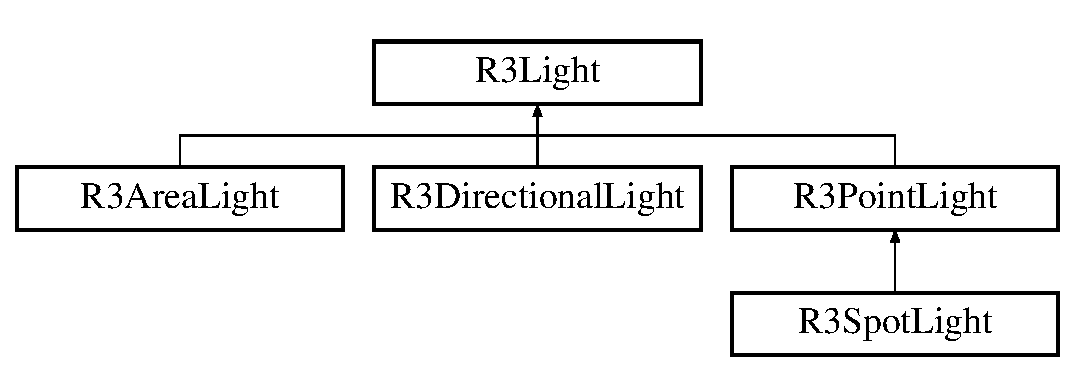
\includegraphics[height=3.000000cm]{class_r3_light}
\end{center}
\end{figure}
\subsection*{Public Member Functions}
\begin{DoxyCompactItemize}
\item 
{\bfseries R3\+Light} (const \hyperlink{class_r3_light}{R3\+Light} \&light)\hypertarget{class_r3_light_add6fecb84c797c512ca9566f1bd38ffe}{}\label{class_r3_light_add6fecb84c797c512ca9566f1bd38ffe}

\item 
{\bfseries R3\+Light} (const \hyperlink{class_r_n_rgb}{R\+N\+Rgb} \&color, R\+N\+Scalar intensity=1.\+0, R\+N\+Boolean active=T\+R\+UE)\hypertarget{class_r3_light_aad9f988b6d6b5bc0aabf7f0e351265b7}{}\label{class_r3_light_aad9f988b6d6b5bc0aabf7f0e351265b7}

\item 
const R\+N\+Boolean {\bfseries Is\+Active} (void) const \hypertarget{class_r3_light_ae7a1dd4aec471248036f813710b0c556}{}\label{class_r3_light_ae7a1dd4aec471248036f813710b0c556}

\item 
const R\+N\+Scalar {\bfseries Intensity} (void) const \hypertarget{class_r3_light_a69f41c26e429ae91ca381b9ae94a5723}{}\label{class_r3_light_a69f41c26e429ae91ca381b9ae94a5723}

\item 
const \hyperlink{class_r_n_rgb}{R\+N\+Rgb} \& {\bfseries Color} (void) const \hypertarget{class_r3_light_a514bcc5f8b6174ea86f9e5c9d47e90b9}{}\label{class_r3_light_a514bcc5f8b6174ea86f9e5c9d47e90b9}

\item 
virtual void {\bfseries Set\+Active} (R\+N\+Boolean active)\hypertarget{class_r3_light_a3e63231405abc3733faad292319c6294}{}\label{class_r3_light_a3e63231405abc3733faad292319c6294}

\item 
virtual void {\bfseries Set\+Intensity} (R\+N\+Scalar intensity)\hypertarget{class_r3_light_afe46e426b3e9223083fdbb8f6b9b943f}{}\label{class_r3_light_afe46e426b3e9223083fdbb8f6b9b943f}

\item 
virtual void {\bfseries Set\+Color} (const \hyperlink{class_r_n_rgb}{R\+N\+Rgb} \&color)\hypertarget{class_r3_light_a66d85f36dc01ae14fd5bbcc5484fcc24}{}\label{class_r3_light_a66d85f36dc01ae14fd5bbcc5484fcc24}

\item 
virtual \hyperlink{class_r_n_rgb}{R\+N\+Rgb} {\bfseries Reflection} (const \hyperlink{class_r3_brdf}{R3\+Brdf} \&brdf, const \hyperlink{class_r3_point}{R3\+Point} \&eye, const \hyperlink{class_r3_point}{R3\+Point} \&point, const \hyperlink{class_r3_vector}{R3\+Vector} \&normal) const  =0\hypertarget{class_r3_light_a1a71a0fe232ccb31beeb50d713b875c3}{}\label{class_r3_light_a1a71a0fe232ccb31beeb50d713b875c3}

\item 
virtual \hyperlink{class_r_n_rgb}{R\+N\+Rgb} {\bfseries Diffuse\+Reflection} (const \hyperlink{class_r3_brdf}{R3\+Brdf} \&brdf, const \hyperlink{class_r3_point}{R3\+Point} \&point, const \hyperlink{class_r3_vector}{R3\+Vector} \&normal) const  =0\hypertarget{class_r3_light_a0a0bf1256434ae1b56b659f1745b471c}{}\label{class_r3_light_a0a0bf1256434ae1b56b659f1745b471c}

\item 
virtual \hyperlink{class_r_n_rgb}{R\+N\+Rgb} {\bfseries Specular\+Reflection} (const \hyperlink{class_r3_brdf}{R3\+Brdf} \&brdf, const \hyperlink{class_r3_point}{R3\+Point} \&eye, const \hyperlink{class_r3_point}{R3\+Point} \&point, const \hyperlink{class_r3_vector}{R3\+Vector} \&normal) const  =0\hypertarget{class_r3_light_a32483a1d021730650d5fb4b923c09ee2}{}\label{class_r3_light_a32483a1d021730650d5fb4b923c09ee2}

\item 
virtual void {\bfseries Draw} (int i) const  =0\hypertarget{class_r3_light_acab9d89b70c14ca4af5b702a3c00c4b9}{}\label{class_r3_light_acab9d89b70c14ca4af5b702a3c00c4b9}

\item 
{\bfseries R\+N\+\_\+\+C\+L\+A\+S\+S\+\_\+\+T\+Y\+P\+E\+\_\+\+D\+E\+C\+L\+A\+R\+A\+T\+I\+O\+NS} (\hyperlink{class_r3_light}{R3\+Light})\hypertarget{class_r3_light_a14375a14186352b654dc75885dd02832}{}\label{class_r3_light_a14375a14186352b654dc75885dd02832}

\end{DoxyCompactItemize}


The documentation for this class was generated from the following files\+:\begin{DoxyCompactItemize}
\item 
R3\+Graphics/R3\+Light.\+h\item 
R3\+Graphics/R3\+Light.\+cpp\end{DoxyCompactItemize}

\hypertarget{class_r3_line}{}\section{R3\+Line Class Reference}
\label{class_r3_line}\index{R3\+Line@{R3\+Line}}
\subsection*{Public Member Functions}
\begin{DoxyCompactItemize}
\item 
{\bfseries R3\+Line} (const \hyperlink{class_r3_line}{R3\+Line} \&line)\hypertarget{class_r3_line_a6c4e21cb05b9d18fe2fb2e27e9f2c0f5}{}\label{class_r3_line_a6c4e21cb05b9d18fe2fb2e27e9f2c0f5}

\item 
{\bfseries R3\+Line} (const \hyperlink{class_r3_point}{R3\+Point} \&point, const \hyperlink{class_r3_vector}{R3\+Vector} \&vector, R\+N\+Boolean normalized=F\+A\+L\+SE)\hypertarget{class_r3_line_a11322e14233c2097c16b0ee04f0f0d6d}{}\label{class_r3_line_a11322e14233c2097c16b0ee04f0f0d6d}

\item 
{\bfseries R3\+Line} (const \hyperlink{class_r3_point}{R3\+Point} \&point1, const \hyperlink{class_r3_point}{R3\+Point} \&point2)\hypertarget{class_r3_line_a1c3121d6d0aab241b7d4422bed57b76d}{}\label{class_r3_line_a1c3121d6d0aab241b7d4422bed57b76d}

\item 
{\bfseries R3\+Line} (R\+N\+Coord x1, R\+N\+Coord y1, R\+N\+Coord z1, R\+N\+Coord x2, R\+N\+Coord y2, R\+N\+Coord z2)\hypertarget{class_r3_line_ae46d218409e58b60c0acede0b78bd9e2}{}\label{class_r3_line_ae46d218409e58b60c0acede0b78bd9e2}

\item 
{\bfseries R3\+Line} (const \hyperlink{class_r_n_array}{R\+N\+Array}$<$ \hyperlink{class_r3_point}{R3\+Point} $\ast$ $>$ \&points)\hypertarget{class_r3_line_a4a729fef4fdef20ff4d93e4afa8aade9}{}\label{class_r3_line_a4a729fef4fdef20ff4d93e4afa8aade9}

\item 
{\bfseries R3\+Line} (\hyperlink{class_r3_point}{R3\+Point} $\ast$points, int npoints)\hypertarget{class_r3_line_a1b6d30aeeb34ebdf0e720b9f3292b5be}{}\label{class_r3_line_a1b6d30aeeb34ebdf0e720b9f3292b5be}

\item 
const \hyperlink{class_r3_point}{R3\+Point} \& {\bfseries Point} (void) const \hypertarget{class_r3_line_a5a9252b71fdb385f5e61ee2769627ce7}{}\label{class_r3_line_a5a9252b71fdb385f5e61ee2769627ce7}

\item 
const \hyperlink{class_r3_vector}{R3\+Vector} \& {\bfseries Vector} (void) const \hypertarget{class_r3_line_a20b743a4d94e001acfc6622663c12165}{}\label{class_r3_line_a20b743a4d94e001acfc6622663c12165}

\item 
const R\+N\+Boolean {\bfseries Is\+Zero} (void) const \hypertarget{class_r3_line_a3b5c9a967f4adb299d5347280fb5b5b3}{}\label{class_r3_line_a3b5c9a967f4adb299d5347280fb5b5b3}

\item 
const R\+N\+Boolean {\bfseries operator==} (const \hyperlink{class_r3_line}{R3\+Line} \&line) const \hypertarget{class_r3_line_aef63e2697ea3b21f34499bd942694aa3}{}\label{class_r3_line_aef63e2697ea3b21f34499bd942694aa3}

\item 
const R\+N\+Boolean {\bfseries operator!=} (const \hyperlink{class_r3_line}{R3\+Line} \&line) const \hypertarget{class_r3_line_a2f21ac8a72d7138223ff10d1fd686a71}{}\label{class_r3_line_a2f21ac8a72d7138223ff10d1fd686a71}

\item 
void {\bfseries Flip} (void)\hypertarget{class_r3_line_a7afcac685ab61af341f88bc4894e89f5}{}\label{class_r3_line_a7afcac685ab61af341f88bc4894e89f5}

\item 
void {\bfseries Mirror} (const \hyperlink{class_r3_plane}{R3\+Plane} \&plane)\hypertarget{class_r3_line_a54683065aa06b7326365f26796d23f80}{}\label{class_r3_line_a54683065aa06b7326365f26796d23f80}

\item 
void {\bfseries Translate} (const \hyperlink{class_r3_vector}{R3\+Vector} \&vector)\hypertarget{class_r3_line_ae7e070736bfc965deb322e892b485c9f}{}\label{class_r3_line_ae7e070736bfc965deb322e892b485c9f}

\item 
void {\bfseries Reposition} (const \hyperlink{class_r3_point}{R3\+Point} \&point)\hypertarget{class_r3_line_a1e05001e880d5f6dbef08fd51df0caa8}{}\label{class_r3_line_a1e05001e880d5f6dbef08fd51df0caa8}

\item 
void {\bfseries Align} (const \hyperlink{class_r3_vector}{R3\+Vector} \&vector, R\+N\+Boolean normalized=F\+A\+L\+SE)\hypertarget{class_r3_line_aa77b45f257b933ca0f2aa9df6a2213b2}{}\label{class_r3_line_aa77b45f257b933ca0f2aa9df6a2213b2}

\item 
void {\bfseries Transform} (const \hyperlink{class_r3_transformation}{R3\+Transformation} \&transformation)\hypertarget{class_r3_line_a26164e52f532f2ec0fcc2ffe60b4df5f}{}\label{class_r3_line_a26164e52f532f2ec0fcc2ffe60b4df5f}

\item 
void {\bfseries Inverse\+Transform} (const \hyperlink{class_r3_transformation}{R3\+Transformation} \&transformation)\hypertarget{class_r3_line_adcc394f67441dab5d2202442d407531f}{}\label{class_r3_line_adcc394f67441dab5d2202442d407531f}

\item 
void {\bfseries Reset} (const \hyperlink{class_r3_point}{R3\+Point} \&point, const \hyperlink{class_r3_vector}{R3\+Vector} \&vector, R\+N\+Boolean normalized=F\+A\+L\+SE)\hypertarget{class_r3_line_a8d9fea53e35a2c344fd985d223e0f8cc}{}\label{class_r3_line_a8d9fea53e35a2c344fd985d223e0f8cc}

\item 
void {\bfseries Draw} (void) const \hypertarget{class_r3_line_ac3aada07f6f35c5839e97a8077feb2cd}{}\label{class_r3_line_ac3aada07f6f35c5839e97a8077feb2cd}

\item 
\hyperlink{class_r3_line}{R3\+Line} {\bfseries operator-\/} (void) const \hypertarget{class_r3_line_a02c3e798e6a72d80db686be9ed3e99ec}{}\label{class_r3_line_a02c3e798e6a72d80db686be9ed3e99ec}

\end{DoxyCompactItemize}


The documentation for this class was generated from the following files\+:\begin{DoxyCompactItemize}
\item 
R3\+Shapes/R3\+Line.\+h\item 
R3\+Shapes/R3\+Draw.\+cpp\item 
R3\+Shapes/R3\+Line.\+cpp\end{DoxyCompactItemize}

\hypertarget{class_r3_material}{}\section{R3\+Material Class Reference}
\label{class_r3_material}\index{R3\+Material@{R3\+Material}}
\subsection*{Public Member Functions}
\begin{DoxyCompactItemize}
\item 
{\bfseries R3\+Material} (const char $\ast$name=N\+U\+LL)\hypertarget{class_r3_material_a07cc8021d12cd084c709798ac2b1c214}{}\label{class_r3_material_a07cc8021d12cd084c709798ac2b1c214}

\item 
{\bfseries R3\+Material} (const \hyperlink{class_r3_material}{R3\+Material} \&material)\hypertarget{class_r3_material_ace2993b7f61e76a7c53c7038e79a9752}{}\label{class_r3_material_ace2993b7f61e76a7c53c7038e79a9752}

\item 
{\bfseries R3\+Material} (const \hyperlink{class_r3_brdf}{R3\+Brdf} $\ast$brdf, const char $\ast$name=N\+U\+LL)\hypertarget{class_r3_material_a066b8fd2496c45c9fe0c33c077df7cc0}{}\label{class_r3_material_a066b8fd2496c45c9fe0c33c077df7cc0}

\item 
{\bfseries R3\+Material} (const \hyperlink{class_r2_texture}{R2\+Texture} $\ast$texture, const char $\ast$name=N\+U\+LL)\hypertarget{class_r3_material_a05b024ad05df03be1040d1736a295171}{}\label{class_r3_material_a05b024ad05df03be1040d1736a295171}

\item 
{\bfseries R3\+Material} (const \hyperlink{class_r3_brdf}{R3\+Brdf} $\ast$brdf, const \hyperlink{class_r2_texture}{R2\+Texture} $\ast$texture, const char $\ast$name=N\+U\+LL)\hypertarget{class_r3_material_acdcf7f2392e1786bc737de2433946944}{}\label{class_r3_material_acdcf7f2392e1786bc737de2433946944}

\item 
const char $\ast$ {\bfseries Name} (void) const \hypertarget{class_r3_material_a33a317c070cb380e4935e053446596f2}{}\label{class_r3_material_a33a317c070cb380e4935e053446596f2}

\item 
const \hyperlink{class_r3_brdf}{R3\+Brdf} $\ast$ {\bfseries Brdf} (void) const \hypertarget{class_r3_material_a24d172de895eb1e8d155989614a262f5}{}\label{class_r3_material_a24d172de895eb1e8d155989614a262f5}

\item 
const \hyperlink{class_r2_texture}{R2\+Texture} $\ast$ {\bfseries Texture} (void) const \hypertarget{class_r3_material_adb3b9725fc7ff3e0daf1f5e89dff8658}{}\label{class_r3_material_adb3b9725fc7ff3e0daf1f5e89dff8658}

\item 
const \hyperlink{class_r_n_flags}{R\+N\+Flags} \& {\bfseries Flags} (void) const \hypertarget{class_r3_material_a0348d7a761c37a72bcb7c214f095073b}{}\label{class_r3_material_a0348d7a761c37a72bcb7c214f095073b}

\item 
const R\+N\+Boolean {\bfseries Is\+Reflective} (void) const \hypertarget{class_r3_material_acf58b1ee4d1a08b066955d59c138cb70}{}\label{class_r3_material_acf58b1ee4d1a08b066955d59c138cb70}

\item 
const R\+N\+Boolean {\bfseries Is\+Ambient} (void) const \hypertarget{class_r3_material_a82a247481e72713014ac9f94fe27c7f7}{}\label{class_r3_material_a82a247481e72713014ac9f94fe27c7f7}

\item 
const R\+N\+Boolean {\bfseries Is\+Diffuse} (void) const \hypertarget{class_r3_material_a10a6578179e33218ffa010294fc1e88f}{}\label{class_r3_material_a10a6578179e33218ffa010294fc1e88f}

\item 
const R\+N\+Boolean {\bfseries Is\+Specular} (void) const \hypertarget{class_r3_material_a32a006663fe467228e13abf3c231383b}{}\label{class_r3_material_a32a006663fe467228e13abf3c231383b}

\item 
const R\+N\+Boolean {\bfseries Is\+Emissive} (void) const \hypertarget{class_r3_material_ac292d967e66c07b8e90881fab4cee70a}{}\label{class_r3_material_ac292d967e66c07b8e90881fab4cee70a}

\item 
const R\+N\+Boolean {\bfseries Is\+Shiny} (void) const \hypertarget{class_r3_material_ab747edeebfbe699fddcff4bed5ab70d3}{}\label{class_r3_material_ab747edeebfbe699fddcff4bed5ab70d3}

\item 
const R\+N\+Boolean {\bfseries Is\+Textured} (void) const \hypertarget{class_r3_material_ae747e8213c83acdb22a759e8ac510936}{}\label{class_r3_material_ae747e8213c83acdb22a759e8ac510936}

\item 
const R\+N\+Boolean {\bfseries Is\+Transparent} (void) const \hypertarget{class_r3_material_a7826c12b8a09baa641528d5e8f6baf9d}{}\label{class_r3_material_a7826c12b8a09baa641528d5e8f6baf9d}

\item 
\hyperlink{class_r3_material}{R3\+Material} \& {\bfseries operator=} (const \hyperlink{class_r3_material}{R3\+Material} \&material)\hypertarget{class_r3_material_a93047a9220941fff5885c0e5274378fc}{}\label{class_r3_material_a93047a9220941fff5885c0e5274378fc}

\item 
void {\bfseries Set\+Brdf} (const \hyperlink{class_r3_brdf}{R3\+Brdf} $\ast$brdf)\hypertarget{class_r3_material_a7617d0b887a214d2d794c11b3273cea9}{}\label{class_r3_material_a7617d0b887a214d2d794c11b3273cea9}

\item 
void {\bfseries Set\+Texture} (const \hyperlink{class_r2_texture}{R2\+Texture} $\ast$texture)\hypertarget{class_r3_material_aaaf20e075d37fbf2c504e3f5f7a82ad5}{}\label{class_r3_material_aaaf20e075d37fbf2c504e3f5f7a82ad5}

\item 
void {\bfseries Set\+Name} (const char $\ast$name)\hypertarget{class_r3_material_ad19d535b2a41ac81586404c8290f7358}{}\label{class_r3_material_ad19d535b2a41ac81586404c8290f7358}

\item 
void {\bfseries Load} (void) const \hypertarget{class_r3_material_afd6eceb62d8e0ffaa4ab97cba06f77c6}{}\label{class_r3_material_afd6eceb62d8e0ffaa4ab97cba06f77c6}

\item 
void {\bfseries Unload} (void) const \hypertarget{class_r3_material_ad9a302b69336d6d73eb0ed3bbd04abc4}{}\label{class_r3_material_ad9a302b69336d6d73eb0ed3bbd04abc4}

\item 
void {\bfseries Draw} (R\+N\+Boolean force=F\+A\+L\+SE) const \hypertarget{class_r3_material_ab7a8baf4b8a8307d7a875085189df145}{}\label{class_r3_material_ab7a8baf4b8a8307d7a875085189df145}

\item 
void {\bfseries Update} (void)\hypertarget{class_r3_material_a1486a2b33bd10f9a44f04088c0905809}{}\label{class_r3_material_a1486a2b33bd10f9a44f04088c0905809}

\end{DoxyCompactItemize}


The documentation for this class was generated from the following files\+:\begin{DoxyCompactItemize}
\item 
R3\+Graphics/R3\+Material.\+h\item 
R3\+Graphics/R3\+Material.\+cpp\end{DoxyCompactItemize}

\hypertarget{class_r3_matrix}{}\section{R3\+Matrix Class Reference}
\label{class_r3_matrix}\index{R3\+Matrix@{R3\+Matrix}}
\subsection*{Public Member Functions}
\begin{DoxyCompactItemize}
\item 
{\bfseries R3\+Matrix} (const \hyperlink{class_r3_matrix}{R3\+Matrix} \&matrix)\hypertarget{class_r3_matrix_a83409b13cc8ff8803d4a9b4b764fdfb4}{}\label{class_r3_matrix_a83409b13cc8ff8803d4a9b4b764fdfb4}

\item 
{\bfseries R3\+Matrix} (R\+N\+Scalar a00, R\+N\+Scalar a01, R\+N\+Scalar a02, R\+N\+Scalar a10, R\+N\+Scalar a11, R\+N\+Scalar a12, R\+N\+Scalar a20, R\+N\+Scalar a21, R\+N\+Scalar a22)\hypertarget{class_r3_matrix_a547e15cf503b2b1f44a1ed58fe8af21b}{}\label{class_r3_matrix_a547e15cf503b2b1f44a1ed58fe8af21b}

\item 
{\bfseries R3\+Matrix} (const R\+N\+Scalar $\ast$array)\hypertarget{class_r3_matrix_a058aafb47d11fb533092c056328414bf}{}\label{class_r3_matrix_a058aafb47d11fb533092c056328414bf}

\item 
const int {\bfseries Is\+Zero} (void) const \hypertarget{class_r3_matrix_ac31565aac506d671a9e624ba4051acb0}{}\label{class_r3_matrix_ac31565aac506d671a9e624ba4051acb0}

\item 
const int {\bfseries Is\+Identity} (void) const \hypertarget{class_r3_matrix_a88d77400a75a67798d56c30f453a394f}{}\label{class_r3_matrix_a88d77400a75a67798d56c30f453a394f}

\item 
const R\+N\+Boolean {\bfseries Is\+Isotropic} (void) const \hypertarget{class_r3_matrix_a6cfef6a3bf1b018bd6983573c5372504}{}\label{class_r3_matrix_a6cfef6a3bf1b018bd6983573c5372504}

\item 
const R\+N\+Boolean {\bfseries Has\+Translation} (void) const \hypertarget{class_r3_matrix_a678d70209a04dbc56d32b0df99312e3d}{}\label{class_r3_matrix_a678d70209a04dbc56d32b0df99312e3d}

\item 
const R\+N\+Boolean {\bfseries Has\+Scale} (void) const \hypertarget{class_r3_matrix_a428edf9f7a7bc5ecc8c6147a553e7846}{}\label{class_r3_matrix_a428edf9f7a7bc5ecc8c6147a553e7846}

\item 
const R\+N\+Boolean {\bfseries Has\+Rotation} (void) const \hypertarget{class_r3_matrix_acdaf3793d0ed307a667c6d2a998a090e}{}\label{class_r3_matrix_acdaf3793d0ed307a667c6d2a998a090e}

\item 
const R\+N\+Boolean {\bfseries Has\+Mirror} (void) const \hypertarget{class_r3_matrix_ac6bbc656edd59822526365612840fea2}{}\label{class_r3_matrix_ac6bbc656edd59822526365612840fea2}

\item 
const R\+N\+Scalar $\ast$ {\bfseries operator\mbox{[}$\,$\mbox{]}} (int i) const \hypertarget{class_r3_matrix_a0d978a68d81255531b62cd7f045b1920}{}\label{class_r3_matrix_a0d978a68d81255531b62cd7f045b1920}

\item 
const R\+N\+Scalar {\bfseries Determinant} (void) const \hypertarget{class_r3_matrix_a8ce7cf291f0cadafe08928873af0045f}{}\label{class_r3_matrix_a8ce7cf291f0cadafe08928873af0045f}

\item 
const \hyperlink{class_r3_matrix}{R3\+Matrix} {\bfseries Transpose} (void) const \hypertarget{class_r3_matrix_a90d380b728dcdc3fc7c4cfc03af2b5da}{}\label{class_r3_matrix_a90d380b728dcdc3fc7c4cfc03af2b5da}

\item 
const \hyperlink{class_r3_matrix}{R3\+Matrix} {\bfseries Inverse} (void) const \hypertarget{class_r3_matrix_a5d873d4dc9d6093034ad1838812722a7}{}\label{class_r3_matrix_a5d873d4dc9d6093034ad1838812722a7}

\item 
const R\+N\+Boolean {\bfseries operator==} (const \hyperlink{class_r3_matrix}{R3\+Matrix} \&matrix) const \hypertarget{class_r3_matrix_a262aaf12efdc03977d8042d21ea38319}{}\label{class_r3_matrix_a262aaf12efdc03977d8042d21ea38319}

\item 
const R\+N\+Boolean {\bfseries operator!=} (const \hyperlink{class_r3_matrix}{R3\+Matrix} \&matrix) const \hypertarget{class_r3_matrix_af8fae6c03a53fbe1e372f08eb8055206}{}\label{class_r3_matrix_af8fae6c03a53fbe1e372f08eb8055206}

\item 
void {\bfseries Flip} (void)\hypertarget{class_r3_matrix_adab13804223f47f3ddbd9a16f989100e}{}\label{class_r3_matrix_adab13804223f47f3ddbd9a16f989100e}

\item 
void {\bfseries Invert} (void)\hypertarget{class_r3_matrix_a15df9d3f499255462b9840ff1a71906f}{}\label{class_r3_matrix_a15df9d3f499255462b9840ff1a71906f}

\item 
void {\bfseries X\+Translate} (R\+N\+Scalar offset)\hypertarget{class_r3_matrix_aa63c6da972cf35c48b9929f2a812dc0c}{}\label{class_r3_matrix_aa63c6da972cf35c48b9929f2a812dc0c}

\item 
void {\bfseries Y\+Translate} (R\+N\+Scalar offset)\hypertarget{class_r3_matrix_a549255b7b1c092452bbc8a0cbf371f8b}{}\label{class_r3_matrix_a549255b7b1c092452bbc8a0cbf371f8b}

\item 
void {\bfseries Translate} (R\+N\+Scalar offset)\hypertarget{class_r3_matrix_a19af9c74b0d99ede124294c4ac5680b0}{}\label{class_r3_matrix_a19af9c74b0d99ede124294c4ac5680b0}

\item 
void {\bfseries Translate} (R\+N\+Axis axis, R\+N\+Scalar offset)\hypertarget{class_r3_matrix_af1185d947fa58276242861d7f76e0f2b}{}\label{class_r3_matrix_af1185d947fa58276242861d7f76e0f2b}

\item 
void {\bfseries Translate} (const \hyperlink{class_r2_vector}{R2\+Vector} \&offset)\hypertarget{class_r3_matrix_a64b7c57d19ff927939fd59f31b32c456}{}\label{class_r3_matrix_a64b7c57d19ff927939fd59f31b32c456}

\item 
void {\bfseries X\+Scale} (R\+N\+Scalar scale)\hypertarget{class_r3_matrix_ae99d1c9ffeb480f0523aaa1f9b1cb862}{}\label{class_r3_matrix_ae99d1c9ffeb480f0523aaa1f9b1cb862}

\item 
void {\bfseries Y\+Scale} (R\+N\+Scalar scale)\hypertarget{class_r3_matrix_a8b5559a983f040223a274bafc73b3419}{}\label{class_r3_matrix_a8b5559a983f040223a274bafc73b3419}

\item 
void {\bfseries Scale} (R\+N\+Scalar scale)\hypertarget{class_r3_matrix_a2a0f429c0c43232bf251d510453de12e}{}\label{class_r3_matrix_a2a0f429c0c43232bf251d510453de12e}

\item 
void {\bfseries Scale} (R\+N\+Axis axis, R\+N\+Scalar scale)\hypertarget{class_r3_matrix_a0d8b42302648658e76b04db2430a223b}{}\label{class_r3_matrix_a0d8b42302648658e76b04db2430a223b}

\item 
void {\bfseries Scale} (const \hyperlink{class_r2_vector}{R2\+Vector} \&scale)\hypertarget{class_r3_matrix_acd3cacba1c6608d033d78cf8d0c4442c}{}\label{class_r3_matrix_acd3cacba1c6608d033d78cf8d0c4442c}

\item 
void {\bfseries Rotate} (R\+N\+Angle radians)\hypertarget{class_r3_matrix_a0d551b8a34d36c70aa433be9097f8908}{}\label{class_r3_matrix_a0d551b8a34d36c70aa433be9097f8908}

\item 
void {\bfseries Transform} (const \hyperlink{class_r3_matrix}{R3\+Matrix} \&matrix)\hypertarget{class_r3_matrix_aa7e75ec6ea66778ba31ec5d9588cb065}{}\label{class_r3_matrix_aa7e75ec6ea66778ba31ec5d9588cb065}

\item 
void {\bfseries Multiply} (const \hyperlink{class_r3_matrix}{R3\+Matrix} \&matrix)\hypertarget{class_r3_matrix_a757cbb898a0d3d8d1ed628b101d0a1a4}{}\label{class_r3_matrix_a757cbb898a0d3d8d1ed628b101d0a1a4}

\item 
void {\bfseries Add} (const \hyperlink{class_r3_matrix}{R3\+Matrix} \&matrix)\hypertarget{class_r3_matrix_a03972a861819b531a0626e0b9f7ea302}{}\label{class_r3_matrix_a03972a861819b531a0626e0b9f7ea302}

\item 
void {\bfseries Subtract} (const \hyperlink{class_r3_matrix}{R3\+Matrix} \&matrix)\hypertarget{class_r3_matrix_a586c07bad57e82f870f71f41428dd68e}{}\label{class_r3_matrix_a586c07bad57e82f870f71f41428dd68e}

\item 
\hyperlink{class_r3_matrix}{R3\+Matrix} \& {\bfseries operator=} (const \hyperlink{class_r3_matrix}{R3\+Matrix} \&matrix)\hypertarget{class_r3_matrix_a1ec647a47d2a3bc1d85afa516686bfe7}{}\label{class_r3_matrix_a1ec647a47d2a3bc1d85afa516686bfe7}

\item 
\hyperlink{class_r3_matrix}{R3\+Matrix} \& {\bfseries operator+=} (const \hyperlink{class_r3_matrix}{R3\+Matrix} \&matrix)\hypertarget{class_r3_matrix_a41b6650421b24028befe341dcd7797eb}{}\label{class_r3_matrix_a41b6650421b24028befe341dcd7797eb}

\item 
\hyperlink{class_r3_matrix}{R3\+Matrix} \& {\bfseries operator-\/=} (const \hyperlink{class_r3_matrix}{R3\+Matrix} \&matrix)\hypertarget{class_r3_matrix_aeba9f9968b29c0c3f8f2a039787a0825}{}\label{class_r3_matrix_aeba9f9968b29c0c3f8f2a039787a0825}

\item 
\hyperlink{class_r3_matrix}{R3\+Matrix} \& {\bfseries operator$\ast$=} (R\+N\+Scalar a)\hypertarget{class_r3_matrix_a3a220a5f2496039afa439983161ef6b3}{}\label{class_r3_matrix_a3a220a5f2496039afa439983161ef6b3}

\item 
\hyperlink{class_r3_matrix}{R3\+Matrix} \& {\bfseries operator$\ast$=} (const \hyperlink{class_r3_matrix}{R3\+Matrix} \&matrix)\hypertarget{class_r3_matrix_aa064b337c2695b81b37dcf68e4c322bb}{}\label{class_r3_matrix_aa064b337c2695b81b37dcf68e4c322bb}

\item 
\hyperlink{class_r3_matrix}{R3\+Matrix} \& {\bfseries operator/=} (R\+N\+Scalar a)\hypertarget{class_r3_matrix_ac877b7363f710f1e1866d803745c5bc3}{}\label{class_r3_matrix_ac877b7363f710f1e1866d803745c5bc3}

\item 
void {\bfseries Load} (void) const \hypertarget{class_r3_matrix_afbe0e41d7986e4d542268dfccb1c395c}{}\label{class_r3_matrix_afbe0e41d7986e4d542268dfccb1c395c}

\item 
void {\bfseries Draw} (void) const \hypertarget{class_r3_matrix_a74913abd1299e8ddae761ede872a2bcf}{}\label{class_r3_matrix_a74913abd1299e8ddae761ede872a2bcf}

\item 
void {\bfseries Push} (void) const \hypertarget{class_r3_matrix_a357fbedfa27f5c17fb88aae74709fff5}{}\label{class_r3_matrix_a357fbedfa27f5c17fb88aae74709fff5}

\item 
void {\bfseries Pop} (void) const \hypertarget{class_r3_matrix_af9eaeaa5ed759eadfb048e455b9a3843}{}\label{class_r3_matrix_af9eaeaa5ed759eadfb048e455b9a3843}

\item 
R\+N\+Scalar $\ast$ {\bfseries operator\mbox{[}$\,$\mbox{]}} (int i)\hypertarget{class_r3_matrix_acae72956775433e302a862811db68f3a}{}\label{class_r3_matrix_acae72956775433e302a862811db68f3a}

\end{DoxyCompactItemize}
\subsection*{Friends}
\begin{DoxyCompactItemize}
\item 
\hyperlink{class_r3_matrix}{R3\+Matrix} {\bfseries operator-\/} (const \hyperlink{class_r3_matrix}{R3\+Matrix} \&matrix)\hypertarget{class_r3_matrix_a84ffdd083fd8a0b8fa54cd9f07e2ca03}{}\label{class_r3_matrix_a84ffdd083fd8a0b8fa54cd9f07e2ca03}

\item 
\hyperlink{class_r3_matrix}{R3\+Matrix} {\bfseries operator+} (const \hyperlink{class_r3_matrix}{R3\+Matrix} \&matrix1, const \hyperlink{class_r3_matrix}{R3\+Matrix} \&matrix2)\hypertarget{class_r3_matrix_a19aeaeca6ace1ef0b2320ab13a4c6e3f}{}\label{class_r3_matrix_a19aeaeca6ace1ef0b2320ab13a4c6e3f}

\item 
\hyperlink{class_r3_matrix}{R3\+Matrix} {\bfseries operator-\/} (const \hyperlink{class_r3_matrix}{R3\+Matrix} \&matrix1, const \hyperlink{class_r3_matrix}{R3\+Matrix} \&matrix2)\hypertarget{class_r3_matrix_a5e61dc4eddde46530ee9f455c0e93df1}{}\label{class_r3_matrix_a5e61dc4eddde46530ee9f455c0e93df1}

\item 
\hyperlink{class_r3_matrix}{R3\+Matrix} {\bfseries operator$\ast$} (R\+N\+Scalar a, const \hyperlink{class_r3_matrix}{R3\+Matrix} \&matrix)\hypertarget{class_r3_matrix_a9e92b5ef243bbece37ed080f1fb49aa7}{}\label{class_r3_matrix_a9e92b5ef243bbece37ed080f1fb49aa7}

\item 
\hyperlink{class_r3_matrix}{R3\+Matrix} {\bfseries operator$\ast$} (const \hyperlink{class_r3_matrix}{R3\+Matrix} \&matrix, R\+N\+Scalar a)\hypertarget{class_r3_matrix_a119632e728a127685cfc4fc1d8fc22a2}{}\label{class_r3_matrix_a119632e728a127685cfc4fc1d8fc22a2}

\item 
\hyperlink{class_r3_matrix}{R3\+Matrix} {\bfseries operator$\ast$} (const \hyperlink{class_r3_matrix}{R3\+Matrix} \&matrix1, const \hyperlink{class_r3_matrix}{R3\+Matrix} \&matrix2)\hypertarget{class_r3_matrix_a59635f30234336a3d81f607d10f9e784}{}\label{class_r3_matrix_a59635f30234336a3d81f607d10f9e784}

\item 
\hyperlink{class_r3_matrix}{R3\+Matrix} {\bfseries operator/} (const \hyperlink{class_r3_matrix}{R3\+Matrix} \&matrix, R\+N\+Scalar scale)\hypertarget{class_r3_matrix_a7a5ffa9ddd6528043eda24063ada0dcb}{}\label{class_r3_matrix_a7a5ffa9ddd6528043eda24063ada0dcb}

\item 
\hyperlink{class_r2_vector}{R2\+Vector} {\bfseries operator$\ast$} (const \hyperlink{class_r3_matrix}{R3\+Matrix} \&matrix, const \hyperlink{class_r2_vector}{R2\+Vector} \&vector)\hypertarget{class_r3_matrix_a1c35b832022d76a7123918c7edbe351a}{}\label{class_r3_matrix_a1c35b832022d76a7123918c7edbe351a}

\item 
\hyperlink{class_r2_point}{R2\+Point} {\bfseries operator$\ast$} (const \hyperlink{class_r3_matrix}{R3\+Matrix} \&matrix, const \hyperlink{class_r2_point}{R2\+Point} \&point)\hypertarget{class_r3_matrix_acabce224f46c36b42787b46a1ccaa098}{}\label{class_r3_matrix_acabce224f46c36b42787b46a1ccaa098}

\end{DoxyCompactItemize}


The documentation for this class was generated from the following files\+:\begin{DoxyCompactItemize}
\item 
R2\+Shapes/R3\+Matrix.\+h\item 
R2\+Shapes/R2\+Draw.\+cpp\item 
R2\+Shapes/R3\+Matrix.\+cpp\end{DoxyCompactItemize}

\hypertarget{class_r3_mesh}{}\section{R3\+Mesh Class Reference}
\label{class_r3_mesh}\index{R3\+Mesh@{R3\+Mesh}}
Inheritance diagram for R3\+Mesh\+:\begin{figure}[H]
\begin{center}
\leavevmode
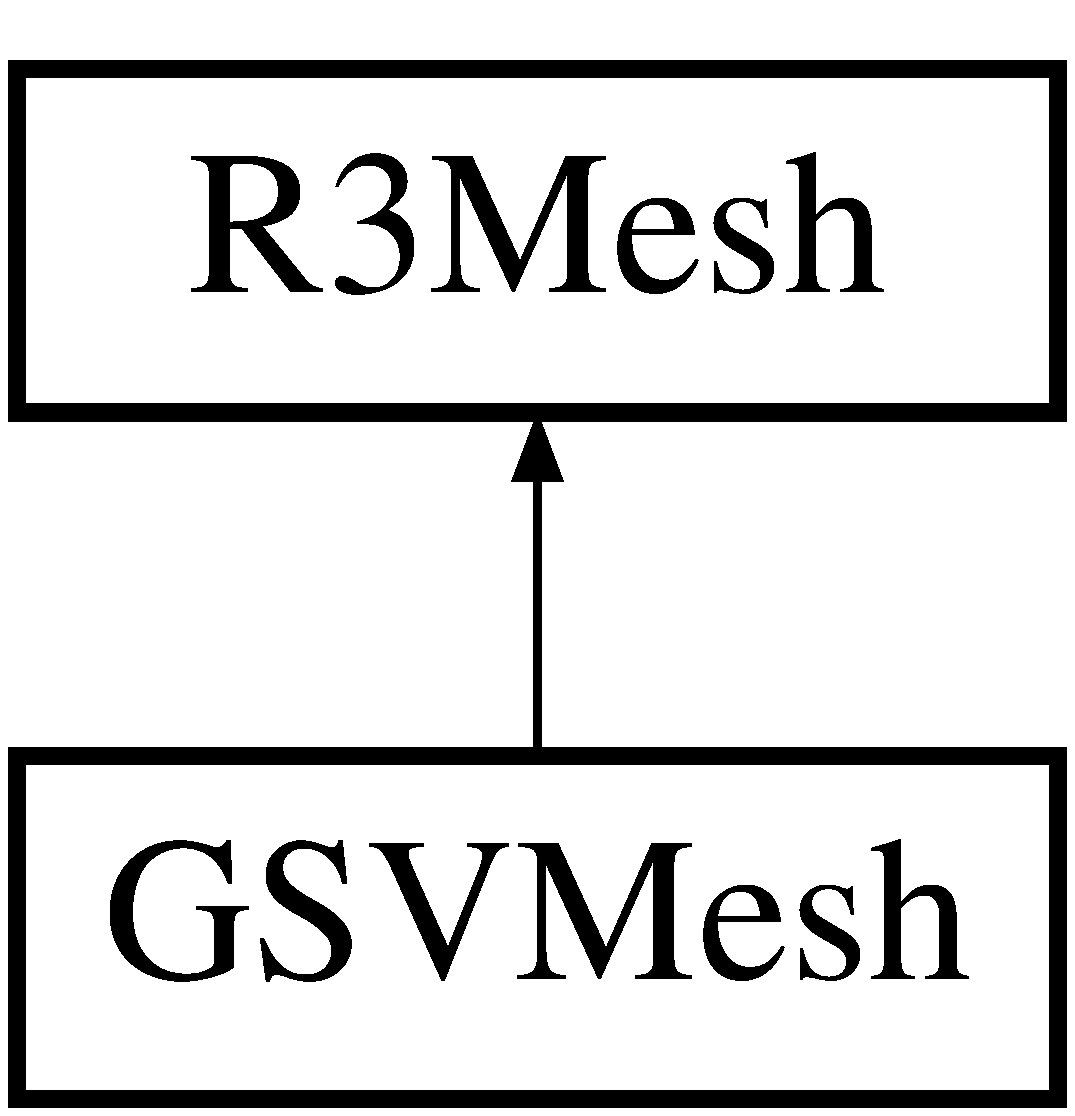
\includegraphics[height=2.000000cm]{class_r3_mesh}
\end{center}
\end{figure}
\subsection*{Public Member Functions}
\begin{DoxyCompactItemize}
\item 
{\bfseries R3\+Mesh} (const \hyperlink{class_r3_mesh}{R3\+Mesh} \&mesh)\hypertarget{class_r3_mesh_a0d6c31f88d1b37d0005bf52c41481828}{}\label{class_r3_mesh_a0d6c31f88d1b37d0005bf52c41481828}

\item 
int {\bfseries N\+Vertices} (void) const \hypertarget{class_r3_mesh_ae76ec0b755d4ed7745fc31695325249f}{}\label{class_r3_mesh_ae76ec0b755d4ed7745fc31695325249f}

\item 
\hyperlink{class_r3_mesh_vertex}{R3\+Mesh\+Vertex} $\ast$ {\bfseries Vertex} (int k) const \hypertarget{class_r3_mesh_a3b76ad274f818b41320fca824d5dff90}{}\label{class_r3_mesh_a3b76ad274f818b41320fca824d5dff90}

\item 
int {\bfseries N\+Edges} (void) const \hypertarget{class_r3_mesh_a547f1863721a2aed724bbb287a159792}{}\label{class_r3_mesh_a547f1863721a2aed724bbb287a159792}

\item 
\hyperlink{class_r3_mesh_edge}{R3\+Mesh\+Edge} $\ast$ {\bfseries Edge} (int k) const \hypertarget{class_r3_mesh_a9769852829f06da31d4e26b5eadc08f6}{}\label{class_r3_mesh_a9769852829f06da31d4e26b5eadc08f6}

\item 
int {\bfseries N\+Faces} (void) const \hypertarget{class_r3_mesh_a2e78b87de5406a315c2a4b7f8d832ac9}{}\label{class_r3_mesh_a2e78b87de5406a315c2a4b7f8d832ac9}

\item 
\hyperlink{class_r3_mesh_face}{R3\+Mesh\+Face} $\ast$ {\bfseries Face} (int k) const \hypertarget{class_r3_mesh_af73a9baad089868c971b3973bae40b19}{}\label{class_r3_mesh_af73a9baad089868c971b3973bae40b19}

\item 
const char $\ast$ {\bfseries Name} (void) const \hypertarget{class_r3_mesh_a8d2f1e847015a9218aa6889977df7425}{}\label{class_r3_mesh_a8d2f1e847015a9218aa6889977df7425}

\item 
const \hyperlink{class_r3_box}{R3\+Box} \& {\bfseries B\+Box} (void) const \hypertarget{class_r3_mesh_afb0b5fec86037876bef5a39b650c7f83}{}\label{class_r3_mesh_afb0b5fec86037876bef5a39b650c7f83}

\item 
\hyperlink{class_r3_point}{R3\+Point} {\bfseries Centroid} (void) const \hypertarget{class_r3_mesh_a0bf2d00f661f921a38698e8adcfc8d9c}{}\label{class_r3_mesh_a0bf2d00f661f921a38698e8adcfc8d9c}

\item 
R\+N\+Area {\bfseries Area} (void) const \hypertarget{class_r3_mesh_a1431bfda55f834837172b98acffe249d}{}\label{class_r3_mesh_a1431bfda55f834837172b98acffe249d}

\item 
R\+N\+Length {\bfseries Average\+Edge\+Length} (void) const \hypertarget{class_r3_mesh_a5001acde8b4b470dcb26823719b43267}{}\label{class_r3_mesh_a5001acde8b4b470dcb26823719b43267}

\item 
R\+N\+Length {\bfseries Average\+Radius} (const \hyperlink{class_r3_point}{R3\+Point} $\ast$centroid=N\+U\+LL) const \hypertarget{class_r3_mesh_ae0c01cea92f71dfaa918c5d082d5c2cc}{}\label{class_r3_mesh_ae0c01cea92f71dfaa918c5d082d5c2cc}

\item 
\hyperlink{class_r3_triad}{R3\+Triad} {\bfseries Principle\+Axes} (const \hyperlink{class_r3_point}{R3\+Point} $\ast$centroid=N\+U\+LL, R\+N\+Scalar $\ast$variances=N\+U\+LL) const \hypertarget{class_r3_mesh_a43e3f1234625c0b651925689c7e51199}{}\label{class_r3_mesh_a43e3f1234625c0b651925689c7e51199}

\item 
\hyperlink{class_r3_affine}{R3\+Affine} {\bfseries P\+C\+A\+Normalization\+Transformation} (R\+N\+Boolean translate=T\+R\+UE, R\+N\+Boolean rotate=T\+R\+UE, R\+N\+Boolean scale=T\+R\+UE) const \hypertarget{class_r3_mesh_a916cc4afe9c3c40474192ecaa18e230d}{}\label{class_r3_mesh_a916cc4afe9c3c40474192ecaa18e230d}

\item 
void $\ast$ {\bfseries Data} (void) const \hypertarget{class_r3_mesh_a3cda384864fe296ea74c06eea88c53a3}{}\label{class_r3_mesh_a3cda384864fe296ea74c06eea88c53a3}

\item 
const \hyperlink{class_r3_point}{R3\+Point} \& {\bfseries Vertex\+Position} (const \hyperlink{class_r3_mesh_vertex}{R3\+Mesh\+Vertex} $\ast$vertex) const \hypertarget{class_r3_mesh_a889925a27cf1b210c5503b1f772ff0b6}{}\label{class_r3_mesh_a889925a27cf1b210c5503b1f772ff0b6}

\item 
const \hyperlink{class_r3_vector}{R3\+Vector} \& {\bfseries Vertex\+Normal} (const \hyperlink{class_r3_mesh_vertex}{R3\+Mesh\+Vertex} $\ast$vertex) const \hypertarget{class_r3_mesh_a923b5dd1304148db8bfa4346dfbd9ca3}{}\label{class_r3_mesh_a923b5dd1304148db8bfa4346dfbd9ca3}

\item 
const \hyperlink{class_r_n_rgb}{R\+N\+Rgb} \& {\bfseries Vertex\+Color} (const \hyperlink{class_r3_mesh_vertex}{R3\+Mesh\+Vertex} $\ast$vertex) const \hypertarget{class_r3_mesh_a9a7adf91cfd0192c3e5ca50ebb0150e8}{}\label{class_r3_mesh_a9a7adf91cfd0192c3e5ca50ebb0150e8}

\item 
R\+N\+Area {\bfseries Vertex\+Area} (const \hyperlink{class_r3_mesh_vertex}{R3\+Mesh\+Vertex} $\ast$vertex) const \hypertarget{class_r3_mesh_ada6bb10e165e677155c75c5963a1dfef}{}\label{class_r3_mesh_ada6bb10e165e677155c75c5963a1dfef}

\item 
\hyperlink{class_r3_plane}{R3\+Plane} {\bfseries Vertex\+Tangent\+Plane} (const \hyperlink{class_r3_mesh_vertex}{R3\+Mesh\+Vertex} $\ast$vertex) const \hypertarget{class_r3_mesh_aeeb61cbad1754fde7d49f598f8d094ec}{}\label{class_r3_mesh_aeeb61cbad1754fde7d49f598f8d094ec}

\item 
R\+N\+Scalar {\bfseries Vertex\+Curvature} (const \hyperlink{class_r3_mesh_vertex}{R3\+Mesh\+Vertex} $\ast$vertex) const \hypertarget{class_r3_mesh_a219aad725f9539397e5257ead59f43c3}{}\label{class_r3_mesh_a219aad725f9539397e5257ead59f43c3}

\item 
R\+N\+Scalar {\bfseries Vertex\+Gauss\+Curvature} (const \hyperlink{class_r3_mesh_vertex}{R3\+Mesh\+Vertex} $\ast$vertex) const \hypertarget{class_r3_mesh_a5658160da7dcecad81de8d6d66ee1ba3}{}\label{class_r3_mesh_a5658160da7dcecad81de8d6d66ee1ba3}

\item 
R\+N\+Scalar {\bfseries Vertex\+Mean\+Curvature} (const \hyperlink{class_r3_mesh_vertex}{R3\+Mesh\+Vertex} $\ast$vertex) const \hypertarget{class_r3_mesh_ae103f92239da939eac4d48976471c6fa}{}\label{class_r3_mesh_ae103f92239da939eac4d48976471c6fa}

\item 
R\+N\+Length {\bfseries Vertex\+Average\+Edge\+Length} (const \hyperlink{class_r3_mesh_vertex}{R3\+Mesh\+Vertex} $\ast$vertex) const \hypertarget{class_r3_mesh_a371c627f2d40d45fe2bbf149d793f635}{}\label{class_r3_mesh_a371c627f2d40d45fe2bbf149d793f635}

\item 
\hyperlink{class_r3_vector}{R3\+Vector} {\bfseries Vertex\+Laplacian\+Vector} (const \hyperlink{class_r3_mesh_vertex}{R3\+Mesh\+Vertex} $\ast$vertex) const \hypertarget{class_r3_mesh_aef07bacbdac010fde3a2e50296a96a2f}{}\label{class_r3_mesh_aef07bacbdac010fde3a2e50296a96a2f}

\item 
int {\bfseries Vertex\+Valence} (const \hyperlink{class_r3_mesh_vertex}{R3\+Mesh\+Vertex} $\ast$vertex) const \hypertarget{class_r3_mesh_a12ae3199e42a7e962fef827c2f4e8591}{}\label{class_r3_mesh_a12ae3199e42a7e962fef827c2f4e8591}

\item 
int {\bfseries Vertex\+ID} (const \hyperlink{class_r3_mesh_vertex}{R3\+Mesh\+Vertex} $\ast$vertex) const \hypertarget{class_r3_mesh_a3eba605dcab0c2b5c4054eb877faff37}{}\label{class_r3_mesh_a3eba605dcab0c2b5c4054eb877faff37}

\item 
\hyperlink{class_r_n_flags}{R\+N\+Flags} {\bfseries Vertex\+Flags} (const \hyperlink{class_r3_mesh_vertex}{R3\+Mesh\+Vertex} $\ast$vertex) const \hypertarget{class_r3_mesh_a7374b730592ab63610ad44278f7d904d}{}\label{class_r3_mesh_a7374b730592ab63610ad44278f7d904d}

\item 
R\+N\+Scalar {\bfseries Vertex\+Value} (const \hyperlink{class_r3_mesh_vertex}{R3\+Mesh\+Vertex} $\ast$vertex) const \hypertarget{class_r3_mesh_a5003ff9c01f4b92398b7403bb85f00bc}{}\label{class_r3_mesh_a5003ff9c01f4b92398b7403bb85f00bc}

\item 
R\+N\+Mark {\bfseries Vertex\+Mark} (const \hyperlink{class_r3_mesh_vertex}{R3\+Mesh\+Vertex} $\ast$vertex) const \hypertarget{class_r3_mesh_a186d1c38fbcde94f463fbd829233865f}{}\label{class_r3_mesh_a186d1c38fbcde94f463fbd829233865f}

\item 
void $\ast$ {\bfseries Vertex\+Data} (const \hyperlink{class_r3_mesh_vertex}{R3\+Mesh\+Vertex} $\ast$vertex) const \hypertarget{class_r3_mesh_af20f0c080ef9ca811d20ee4f7cbda1fb}{}\label{class_r3_mesh_af20f0c080ef9ca811d20ee4f7cbda1fb}

\item 
R\+N\+Length {\bfseries Edge\+Length} (const \hyperlink{class_r3_mesh_edge}{R3\+Mesh\+Edge} $\ast$edge) const \hypertarget{class_r3_mesh_a734318568d8c7a3fbf85758faead3a8b}{}\label{class_r3_mesh_a734318568d8c7a3fbf85758faead3a8b}

\item 
\hyperlink{class_r3_point}{R3\+Point} {\bfseries Edge\+Midpoint} (const \hyperlink{class_r3_mesh_edge}{R3\+Mesh\+Edge} $\ast$edge) const \hypertarget{class_r3_mesh_a14a5d6028d0245437146c49f5b002acd}{}\label{class_r3_mesh_a14a5d6028d0245437146c49f5b002acd}

\item 
R\+N\+Angle {\bfseries Edge\+Interior\+Angle} (const \hyperlink{class_r3_mesh_edge}{R3\+Mesh\+Edge} $\ast$edge) const \hypertarget{class_r3_mesh_ac8c8094c155a9dd01eb6e7e620bc34a8}{}\label{class_r3_mesh_ac8c8094c155a9dd01eb6e7e620bc34a8}

\item 
\hyperlink{class_r3_vector}{R3\+Vector} {\bfseries Edge\+Normal} (const \hyperlink{class_r3_mesh_edge}{R3\+Mesh\+Edge} $\ast$edge) const \hypertarget{class_r3_mesh_a323d930cd1a63adc8bb01298bd57156e}{}\label{class_r3_mesh_a323d930cd1a63adc8bb01298bd57156e}

\item 
R\+N\+Scalar {\bfseries Edge\+Aspect} (const \hyperlink{class_r3_mesh_edge}{R3\+Mesh\+Edge} $\ast$edge) const \hypertarget{class_r3_mesh_a1547259cce0801d7263b302afcdbd0c5}{}\label{class_r3_mesh_a1547259cce0801d7263b302afcdbd0c5}

\item 
\hyperlink{class_r3_vector}{R3\+Vector} {\bfseries Edge\+Vector} (const \hyperlink{class_r3_mesh_edge}{R3\+Mesh\+Edge} $\ast$edge) const \hypertarget{class_r3_mesh_aad036b1fa918e9bf15c2b41d4c711fe7}{}\label{class_r3_mesh_aad036b1fa918e9bf15c2b41d4c711fe7}

\item 
\hyperlink{class_r3_vector}{R3\+Vector} {\bfseries Edge\+Direction} (const \hyperlink{class_r3_mesh_edge}{R3\+Mesh\+Edge} $\ast$edge) const \hypertarget{class_r3_mesh_aaf21c558310ae4318c72d11dc804121a}{}\label{class_r3_mesh_aaf21c558310ae4318c72d11dc804121a}

\item 
\hyperlink{class_r3_span}{R3\+Span} {\bfseries Edge\+Span} (const \hyperlink{class_r3_mesh_edge}{R3\+Mesh\+Edge} $\ast$edge) const \hypertarget{class_r3_mesh_a703a5fa6e945569f85229c394c57c2f5}{}\label{class_r3_mesh_a703a5fa6e945569f85229c394c57c2f5}

\item 
\hyperlink{class_r3_line}{R3\+Line} {\bfseries Edge\+Line} (const \hyperlink{class_r3_mesh_edge}{R3\+Mesh\+Edge} $\ast$edge) const \hypertarget{class_r3_mesh_a9fc0eab27120e7a6c67fd07f9b27cc14}{}\label{class_r3_mesh_a9fc0eab27120e7a6c67fd07f9b27cc14}

\item 
\hyperlink{class_r3_box}{R3\+Box} {\bfseries Edge\+B\+Box} (const \hyperlink{class_r3_mesh_edge}{R3\+Mesh\+Edge} $\ast$edge) const \hypertarget{class_r3_mesh_a58ef7b563e56b675630d5f721aadcb19}{}\label{class_r3_mesh_a58ef7b563e56b675630d5f721aadcb19}

\item 
int {\bfseries Edge\+ID} (const \hyperlink{class_r3_mesh_edge}{R3\+Mesh\+Edge} $\ast$edge) const \hypertarget{class_r3_mesh_a5ce0c3d7e69041d111ffcdaf8fa46286}{}\label{class_r3_mesh_a5ce0c3d7e69041d111ffcdaf8fa46286}

\item 
\hyperlink{class_r_n_flags}{R\+N\+Flags} {\bfseries Edge\+Flags} (const \hyperlink{class_r3_mesh_edge}{R3\+Mesh\+Edge} $\ast$edge) const \hypertarget{class_r3_mesh_a17bb0f96b8b4195bd9e0f6b7bddaad25}{}\label{class_r3_mesh_a17bb0f96b8b4195bd9e0f6b7bddaad25}

\item 
R\+N\+Scalar {\bfseries Edge\+Value} (const \hyperlink{class_r3_mesh_edge}{R3\+Mesh\+Edge} $\ast$edge) const \hypertarget{class_r3_mesh_ac2b6995c6395974fef02af4dec347873}{}\label{class_r3_mesh_ac2b6995c6395974fef02af4dec347873}

\item 
R\+N\+Mark {\bfseries Edge\+Mark} (const \hyperlink{class_r3_mesh_edge}{R3\+Mesh\+Edge} $\ast$edge) const \hypertarget{class_r3_mesh_a5b5a56eec7cc2bdad297e1d03bfd5e7e}{}\label{class_r3_mesh_a5b5a56eec7cc2bdad297e1d03bfd5e7e}

\item 
void $\ast$ {\bfseries Edge\+Data} (const \hyperlink{class_r3_mesh_edge}{R3\+Mesh\+Edge} $\ast$edge) const \hypertarget{class_r3_mesh_a6bc882e05122386cd93323372608efbd}{}\label{class_r3_mesh_a6bc882e05122386cd93323372608efbd}

\item 
const \hyperlink{class_r3_vector}{R3\+Vector} \& {\bfseries Face\+Normal} (const \hyperlink{class_r3_mesh_face}{R3\+Mesh\+Face} $\ast$face) const \hypertarget{class_r3_mesh_a5b7302972ac74ceebbd028989bbd13a2}{}\label{class_r3_mesh_a5b7302972ac74ceebbd028989bbd13a2}

\item 
const \hyperlink{class_r3_plane}{R3\+Plane} \& {\bfseries Face\+Plane} (const \hyperlink{class_r3_mesh_face}{R3\+Mesh\+Face} $\ast$face) const \hypertarget{class_r3_mesh_ac88c83f229b6db00fe71a16832e029ff}{}\label{class_r3_mesh_ac88c83f229b6db00fe71a16832e029ff}

\item 
\hyperlink{class_r3_point}{R3\+Point} {\bfseries Face\+Centroid} (const \hyperlink{class_r3_mesh_face}{R3\+Mesh\+Face} $\ast$face) const \hypertarget{class_r3_mesh_ae10d78367adb416b01974704da391fef}{}\label{class_r3_mesh_ae10d78367adb416b01974704da391fef}

\item 
\hyperlink{class_r3_point}{R3\+Point} {\bfseries Face\+Point} (const \hyperlink{class_r3_mesh_face}{R3\+Mesh\+Face} $\ast$face, R\+N\+Magnitude barycentrics\mbox{[}3\mbox{]}) const \hypertarget{class_r3_mesh_a7fafb76a7ec0671896a137dcbcd32191}{}\label{class_r3_mesh_a7fafb76a7ec0671896a137dcbcd32191}

\item 
\hyperlink{class_r3_point}{R3\+Point} {\bfseries Face\+Barycentric} (const \hyperlink{class_r3_mesh_face}{R3\+Mesh\+Face} $\ast$face, const \hyperlink{class_r3_point}{R3\+Point} \&point) const \hypertarget{class_r3_mesh_abfe9ea664ead23a4101e620de3e4dacd}{}\label{class_r3_mesh_abfe9ea664ead23a4101e620de3e4dacd}

\item 
const \hyperlink{class_r3_box}{R3\+Box} \& {\bfseries Face\+B\+Box} (const \hyperlink{class_r3_mesh_face}{R3\+Mesh\+Face} $\ast$face) const \hypertarget{class_r3_mesh_a2e20aff8ac1f3d3641133ab1ffa17937}{}\label{class_r3_mesh_a2e20aff8ac1f3d3641133ab1ffa17937}

\item 
R\+N\+Area {\bfseries Face\+Area} (const \hyperlink{class_r3_mesh_face}{R3\+Mesh\+Face} $\ast$face) const \hypertarget{class_r3_mesh_aa961eb00854dfce14442108fe4c446cb}{}\label{class_r3_mesh_aa961eb00854dfce14442108fe4c446cb}

\item 
R\+N\+Scalar {\bfseries Face\+Aspect} (const \hyperlink{class_r3_mesh_face}{R3\+Mesh\+Face} $\ast$face) const \hypertarget{class_r3_mesh_a30feeca818464e19db829884c1d1810d}{}\label{class_r3_mesh_a30feeca818464e19db829884c1d1810d}

\item 
int {\bfseries Face\+Material} (const \hyperlink{class_r3_mesh_face}{R3\+Mesh\+Face} $\ast$face) const \hypertarget{class_r3_mesh_a486b906fc12b45e4fcb75a74de1c67c4}{}\label{class_r3_mesh_a486b906fc12b45e4fcb75a74de1c67c4}

\item 
int {\bfseries Face\+Segment} (const \hyperlink{class_r3_mesh_face}{R3\+Mesh\+Face} $\ast$face) const \hypertarget{class_r3_mesh_a9c60c6da60c998efde0911b3638f4e78}{}\label{class_r3_mesh_a9c60c6da60c998efde0911b3638f4e78}

\item 
int {\bfseries Face\+ID} (const \hyperlink{class_r3_mesh_face}{R3\+Mesh\+Face} $\ast$face) const \hypertarget{class_r3_mesh_a1dd33c26bd3f340ce851ed744dc5681c}{}\label{class_r3_mesh_a1dd33c26bd3f340ce851ed744dc5681c}

\item 
\hyperlink{class_r_n_flags}{R\+N\+Flags} {\bfseries Face\+Flags} (const \hyperlink{class_r3_mesh_face}{R3\+Mesh\+Face} $\ast$face) const \hypertarget{class_r3_mesh_ad74b674a8425153dd7a2efef0755ff9c}{}\label{class_r3_mesh_ad74b674a8425153dd7a2efef0755ff9c}

\item 
R\+N\+Scalar {\bfseries Face\+Value} (const \hyperlink{class_r3_mesh_face}{R3\+Mesh\+Face} $\ast$face) const \hypertarget{class_r3_mesh_a06524fba258d4d294f19f621079c6fc8}{}\label{class_r3_mesh_a06524fba258d4d294f19f621079c6fc8}

\item 
R\+N\+Mark {\bfseries Face\+Mark} (const \hyperlink{class_r3_mesh_face}{R3\+Mesh\+Face} $\ast$face) const \hypertarget{class_r3_mesh_a766b1c1ff18ecdb72a1a02b93cb4961e}{}\label{class_r3_mesh_a766b1c1ff18ecdb72a1a02b93cb4961e}

\item 
void $\ast$ {\bfseries Face\+Data} (const \hyperlink{class_r3_mesh_face}{R3\+Mesh\+Face} $\ast$face) const \hypertarget{class_r3_mesh_a62c2b5b91b088723a9e27957b236fc7a}{}\label{class_r3_mesh_a62c2b5b91b088723a9e27957b236fc7a}

\item 
void {\bfseries Set\+Name} (const char $\ast$name)\hypertarget{class_r3_mesh_a1760d7cc850b02a2050b75c07ccdaaa2}{}\label{class_r3_mesh_a1760d7cc850b02a2050b75c07ccdaaa2}

\item 
void {\bfseries Set\+Vertex\+Position} (\hyperlink{class_r3_mesh_vertex}{R3\+Mesh\+Vertex} $\ast$vertex, const \hyperlink{class_r3_point}{R3\+Point} \&position)\hypertarget{class_r3_mesh_ac9a8c8b377f19b9f2156d9aa3ba7d388}{}\label{class_r3_mesh_ac9a8c8b377f19b9f2156d9aa3ba7d388}

\item 
void {\bfseries Set\+Vertex\+Normal} (\hyperlink{class_r3_mesh_vertex}{R3\+Mesh\+Vertex} $\ast$vertex, const \hyperlink{class_r3_vector}{R3\+Vector} \&normal)\hypertarget{class_r3_mesh_a5675803db6c1489e102122de897adb3c}{}\label{class_r3_mesh_a5675803db6c1489e102122de897adb3c}

\item 
void {\bfseries Set\+Vertex\+Color} (\hyperlink{class_r3_mesh_vertex}{R3\+Mesh\+Vertex} $\ast$vertex, const \hyperlink{class_r_n_rgb}{R\+N\+Rgb} \&color)\hypertarget{class_r3_mesh_ac007c0127c53eed24d7d815dc02fb461}{}\label{class_r3_mesh_ac007c0127c53eed24d7d815dc02fb461}

\item 
void {\bfseries Set\+Vertex\+Value} (\hyperlink{class_r3_mesh_vertex}{R3\+Mesh\+Vertex} $\ast$vertex, R\+N\+Scalar value)\hypertarget{class_r3_mesh_a71bbcf55a07661e10a519556b18f2f27}{}\label{class_r3_mesh_a71bbcf55a07661e10a519556b18f2f27}

\item 
void {\bfseries Set\+Vertex\+Mark} (\hyperlink{class_r3_mesh_vertex}{R3\+Mesh\+Vertex} $\ast$vertex, R\+N\+Mark mark)\hypertarget{class_r3_mesh_af750ad6a2dcc946a3075eacd6ada6f07}{}\label{class_r3_mesh_af750ad6a2dcc946a3075eacd6ada6f07}

\item 
void {\bfseries Set\+Vertex\+Data} (\hyperlink{class_r3_mesh_vertex}{R3\+Mesh\+Vertex} $\ast$vertex, void $\ast$data)\hypertarget{class_r3_mesh_a1d9a5797285d0a100aea17e15e6d8792}{}\label{class_r3_mesh_a1d9a5797285d0a100aea17e15e6d8792}

\item 
void {\bfseries Set\+Vertex\+Flags} (\hyperlink{class_r3_mesh_vertex}{R3\+Mesh\+Vertex} $\ast$vertex, \hyperlink{class_r_n_flags}{R\+N\+Flags} flags)\hypertarget{class_r3_mesh_af143afdb1509b8a3240a938f06b4d32f}{}\label{class_r3_mesh_af143afdb1509b8a3240a938f06b4d32f}

\item 
void {\bfseries Set\+Edge\+Mark} (\hyperlink{class_r3_mesh_edge}{R3\+Mesh\+Edge} $\ast$edge, R\+N\+Mark mark)\hypertarget{class_r3_mesh_a2dfc64db951ae072b8a0b05d203a03fe}{}\label{class_r3_mesh_a2dfc64db951ae072b8a0b05d203a03fe}

\item 
void {\bfseries Set\+Edge\+Value} (\hyperlink{class_r3_mesh_edge}{R3\+Mesh\+Edge} $\ast$edge, R\+N\+Scalar value)\hypertarget{class_r3_mesh_ac66a3ee15378d776d4853b4146c7cd31}{}\label{class_r3_mesh_ac66a3ee15378d776d4853b4146c7cd31}

\item 
void {\bfseries Set\+Edge\+Data} (\hyperlink{class_r3_mesh_edge}{R3\+Mesh\+Edge} $\ast$edge, void $\ast$data)\hypertarget{class_r3_mesh_a251fb05abea0e6889de3752ef799e6a1}{}\label{class_r3_mesh_a251fb05abea0e6889de3752ef799e6a1}

\item 
void {\bfseries Set\+Edge\+Flags} (\hyperlink{class_r3_mesh_edge}{R3\+Mesh\+Edge} $\ast$edge, \hyperlink{class_r_n_flags}{R\+N\+Flags} flags)\hypertarget{class_r3_mesh_a5ff1c2bc4bf652a535f075ca421bd662}{}\label{class_r3_mesh_a5ff1c2bc4bf652a535f075ca421bd662}

\item 
void {\bfseries Set\+Face\+Plane} (\hyperlink{class_r3_mesh_face}{R3\+Mesh\+Face} $\ast$face, const \hyperlink{class_r3_plane}{R3\+Plane} \&plane)\hypertarget{class_r3_mesh_a380083a9659d2a85b87b11db3bd3f521}{}\label{class_r3_mesh_a380083a9659d2a85b87b11db3bd3f521}

\item 
void {\bfseries Set\+Face\+Material} (\hyperlink{class_r3_mesh_face}{R3\+Mesh\+Face} $\ast$face, int material)\hypertarget{class_r3_mesh_a36d5b143985d36072ee7ba904b99b05e}{}\label{class_r3_mesh_a36d5b143985d36072ee7ba904b99b05e}

\item 
void {\bfseries Set\+Face\+Segment} (\hyperlink{class_r3_mesh_face}{R3\+Mesh\+Face} $\ast$face, int segment)\hypertarget{class_r3_mesh_a205c6baae4f9497c0ae7b32c9d97c742}{}\label{class_r3_mesh_a205c6baae4f9497c0ae7b32c9d97c742}

\item 
void {\bfseries Set\+Face\+Mark} (\hyperlink{class_r3_mesh_face}{R3\+Mesh\+Face} $\ast$face, R\+N\+Mark mark)\hypertarget{class_r3_mesh_ad56a689642ff5e36b1a272db787b6be6}{}\label{class_r3_mesh_ad56a689642ff5e36b1a272db787b6be6}

\item 
void {\bfseries Set\+Face\+Value} (\hyperlink{class_r3_mesh_face}{R3\+Mesh\+Face} $\ast$face, R\+N\+Scalar value)\hypertarget{class_r3_mesh_a5bf16e6774ec6ae452eccc5172a6f140}{}\label{class_r3_mesh_a5bf16e6774ec6ae452eccc5172a6f140}

\item 
void {\bfseries Set\+Face\+Data} (\hyperlink{class_r3_mesh_face}{R3\+Mesh\+Face} $\ast$face, void $\ast$data)\hypertarget{class_r3_mesh_a1ddd1fdc297456764d66c23d6aa2b882}{}\label{class_r3_mesh_a1ddd1fdc297456764d66c23d6aa2b882}

\item 
void {\bfseries Set\+Face\+Flags} (\hyperlink{class_r3_mesh_face}{R3\+Mesh\+Face} $\ast$face, \hyperlink{class_r_n_flags}{R\+N\+Flags} flags)\hypertarget{class_r3_mesh_a41e38d95b39d9802864483f5d285755e}{}\label{class_r3_mesh_a41e38d95b39d9802864483f5d285755e}

\item 
\hyperlink{class_r3_mesh_vertex}{R3\+Mesh\+Vertex} $\ast$ {\bfseries Vertex\+On\+Vertex} (const \hyperlink{class_r3_mesh_vertex}{R3\+Mesh\+Vertex} $\ast$vertex) const \hypertarget{class_r3_mesh_a2d23eab3e3a11a3ceefdf9d9b784c785}{}\label{class_r3_mesh_a2d23eab3e3a11a3ceefdf9d9b784c785}

\item 
\hyperlink{class_r3_mesh_vertex}{R3\+Mesh\+Vertex} $\ast$ {\bfseries Vertex\+On\+Vertex} (const \hyperlink{class_r3_mesh_vertex}{R3\+Mesh\+Vertex} $\ast$vertex, int k) const \hypertarget{class_r3_mesh_aab218a3e27a545d1c2d9cf95f3412589}{}\label{class_r3_mesh_aab218a3e27a545d1c2d9cf95f3412589}

\item 
\hyperlink{class_r3_mesh_edge}{R3\+Mesh\+Edge} $\ast$ {\bfseries Edge\+On\+Vertex} (const \hyperlink{class_r3_mesh_vertex}{R3\+Mesh\+Vertex} $\ast$vertex) const \hypertarget{class_r3_mesh_a2a1f5aed957916261d12a349b5fea248}{}\label{class_r3_mesh_a2a1f5aed957916261d12a349b5fea248}

\item 
\hyperlink{class_r3_mesh_edge}{R3\+Mesh\+Edge} $\ast$ {\bfseries Edge\+On\+Vertex} (const \hyperlink{class_r3_mesh_vertex}{R3\+Mesh\+Vertex} $\ast$vertex, int k) const \hypertarget{class_r3_mesh_aa236e5d8bf2811febe841851c65017f3}{}\label{class_r3_mesh_aa236e5d8bf2811febe841851c65017f3}

\item 
\hyperlink{class_r3_mesh_edge}{R3\+Mesh\+Edge} $\ast$ {\bfseries Edge\+Between\+Vertices} (const \hyperlink{class_r3_mesh_vertex}{R3\+Mesh\+Vertex} $\ast$vertex1, const \hyperlink{class_r3_mesh_vertex}{R3\+Mesh\+Vertex} $\ast$vertex2) const \hypertarget{class_r3_mesh_a23098625b31f757682507f21ce4dbf2c}{}\label{class_r3_mesh_a23098625b31f757682507f21ce4dbf2c}

\item 
\hyperlink{class_r3_mesh_edge}{R3\+Mesh\+Edge} $\ast$ {\bfseries Edge\+On\+Vertex} (const \hyperlink{class_r3_mesh_vertex}{R3\+Mesh\+Vertex} $\ast$vertex, const \hyperlink{class_r3_mesh_edge}{R3\+Mesh\+Edge} $\ast$edge, R\+N\+Direction dir=R\+N\+\_\+\+C\+CW) const \hypertarget{class_r3_mesh_aac8e649b51dc9204d988802656318c82}{}\label{class_r3_mesh_aac8e649b51dc9204d988802656318c82}

\item 
\hyperlink{class_r3_mesh_edge}{R3\+Mesh\+Edge} $\ast$ {\bfseries Edge\+On\+Vertex} (const \hyperlink{class_r3_mesh_vertex}{R3\+Mesh\+Vertex} $\ast$vertex, const \hyperlink{class_r3_mesh_face}{R3\+Mesh\+Face} $\ast$face, R\+N\+Direction dir=R\+N\+\_\+\+C\+CW) const \hypertarget{class_r3_mesh_a954cbbce11031ae7b9dc2bf46487e1c1}{}\label{class_r3_mesh_a954cbbce11031ae7b9dc2bf46487e1c1}

\item 
\hyperlink{class_r3_mesh_edge}{R3\+Mesh\+Edge} $\ast$ {\bfseries Edge\+Across\+Vertex} (const \hyperlink{class_r3_mesh_vertex}{R3\+Mesh\+Vertex} $\ast$vertex, const \hyperlink{class_r3_mesh_edge}{R3\+Mesh\+Edge} $\ast$edge, const \hyperlink{class_r3_mesh_face}{R3\+Mesh\+Face} $\ast$face) const \hypertarget{class_r3_mesh_ad54461fa7bbcd97dbda2d7f474f59913}{}\label{class_r3_mesh_ad54461fa7bbcd97dbda2d7f474f59913}

\item 
\hyperlink{class_r3_mesh_face}{R3\+Mesh\+Face} $\ast$ {\bfseries Face\+On\+Vertex} (const \hyperlink{class_r3_mesh_vertex}{R3\+Mesh\+Vertex} $\ast$vertex) const \hypertarget{class_r3_mesh_aa0de995e792c99d6d021c712a15a4ef9}{}\label{class_r3_mesh_aa0de995e792c99d6d021c712a15a4ef9}

\item 
\hyperlink{class_r3_mesh_face}{R3\+Mesh\+Face} $\ast$ {\bfseries Face\+Between\+Vertices} (const \hyperlink{class_r3_mesh_vertex}{R3\+Mesh\+Vertex} $\ast$vertex1, const \hyperlink{class_r3_mesh_vertex}{R3\+Mesh\+Vertex} $\ast$vertex2, R\+N\+Direction dir=R\+N\+\_\+\+C\+CW) const \hypertarget{class_r3_mesh_af593f4076a60c96a892ee94ead169448}{}\label{class_r3_mesh_af593f4076a60c96a892ee94ead169448}

\item 
\hyperlink{class_r3_mesh_face}{R3\+Mesh\+Face} $\ast$ {\bfseries Face\+On\+Vertex} (const \hyperlink{class_r3_mesh_vertex}{R3\+Mesh\+Vertex} $\ast$vertex, const \hyperlink{class_r3_mesh_edge}{R3\+Mesh\+Edge} $\ast$edge, R\+N\+Direction dir=R\+N\+\_\+\+C\+CW) const \hypertarget{class_r3_mesh_a81476243eaf8ee16cc1a99d091875de4}{}\label{class_r3_mesh_a81476243eaf8ee16cc1a99d091875de4}

\item 
\hyperlink{class_r3_mesh_face}{R3\+Mesh\+Face} $\ast$ {\bfseries Face\+On\+Vertex} (const \hyperlink{class_r3_mesh_vertex}{R3\+Mesh\+Vertex} $\ast$vertex, const \hyperlink{class_r3_mesh_face}{R3\+Mesh\+Face} $\ast$face, R\+N\+Direction dir=R\+N\+\_\+\+C\+CW) const \hypertarget{class_r3_mesh_ac2119df7d67424761c6a349e523cc180}{}\label{class_r3_mesh_ac2119df7d67424761c6a349e523cc180}

\item 
\hyperlink{class_r3_mesh_vertex}{R3\+Mesh\+Vertex} $\ast$ {\bfseries Vertex\+On\+Edge} (const \hyperlink{class_r3_mesh_edge}{R3\+Mesh\+Edge} $\ast$edge) const \hypertarget{class_r3_mesh_ab9d397658766c50cac5be1008cc51f66}{}\label{class_r3_mesh_ab9d397658766c50cac5be1008cc51f66}

\item 
\hyperlink{class_r3_mesh_vertex}{R3\+Mesh\+Vertex} $\ast$ {\bfseries Vertex\+On\+Edge} (const \hyperlink{class_r3_mesh_edge}{R3\+Mesh\+Edge} $\ast$edge, int k) const \hypertarget{class_r3_mesh_abed5d5f7b6b895e8c68327f10f5ce22a}{}\label{class_r3_mesh_abed5d5f7b6b895e8c68327f10f5ce22a}

\item 
\hyperlink{class_r3_mesh_vertex}{R3\+Mesh\+Vertex} $\ast$ {\bfseries Vertex\+Across\+Edge} (const \hyperlink{class_r3_mesh_edge}{R3\+Mesh\+Edge} $\ast$edge, const \hyperlink{class_r3_mesh_vertex}{R3\+Mesh\+Vertex} $\ast$vertex) const \hypertarget{class_r3_mesh_a5757077d811dec01a4915bc82f16b067}{}\label{class_r3_mesh_a5757077d811dec01a4915bc82f16b067}

\item 
\hyperlink{class_r3_mesh_vertex}{R3\+Mesh\+Vertex} $\ast$ {\bfseries Vertex\+Between\+Edges} (const \hyperlink{class_r3_mesh_edge}{R3\+Mesh\+Edge} $\ast$edge1, const \hyperlink{class_r3_mesh_edge}{R3\+Mesh\+Edge} $\ast$edge2) const \hypertarget{class_r3_mesh_a6111c5a8472a8e12df863a46eb2a2ee5}{}\label{class_r3_mesh_a6111c5a8472a8e12df863a46eb2a2ee5}

\item 
\hyperlink{class_r3_mesh_vertex}{R3\+Mesh\+Vertex} $\ast$ {\bfseries Vertex\+On\+Edge} (const \hyperlink{class_r3_mesh_edge}{R3\+Mesh\+Edge} $\ast$edge, const \hyperlink{class_r3_mesh_face}{R3\+Mesh\+Face} $\ast$face, R\+N\+Direction dir=R\+N\+\_\+\+C\+CW) const \hypertarget{class_r3_mesh_acdbfda6170988f29c38ace182d49d060}{}\label{class_r3_mesh_acdbfda6170988f29c38ace182d49d060}

\item 
\hyperlink{class_r3_mesh_edge}{R3\+Mesh\+Edge} $\ast$ {\bfseries Edge\+On\+Edge} (const \hyperlink{class_r3_mesh_edge}{R3\+Mesh\+Edge} $\ast$edge) const \hypertarget{class_r3_mesh_a1667f29a6651fca2a54314bfd4399d51}{}\label{class_r3_mesh_a1667f29a6651fca2a54314bfd4399d51}

\item 
\hyperlink{class_r3_mesh_edge}{R3\+Mesh\+Edge} $\ast$ {\bfseries Edge\+On\+Edge} (const \hyperlink{class_r3_mesh_edge}{R3\+Mesh\+Edge} $\ast$edge, const \hyperlink{class_r3_mesh_vertex}{R3\+Mesh\+Vertex} $\ast$vertex, R\+N\+Direction dir=R\+N\+\_\+\+C\+CW) const \hypertarget{class_r3_mesh_a641e31e5a7a038daa2832a6be0e9a73f}{}\label{class_r3_mesh_a641e31e5a7a038daa2832a6be0e9a73f}

\item 
\hyperlink{class_r3_mesh_face}{R3\+Mesh\+Face} $\ast$ {\bfseries Face\+On\+Edge} (const \hyperlink{class_r3_mesh_edge}{R3\+Mesh\+Edge} $\ast$edge) const \hypertarget{class_r3_mesh_a6bfcad030d1e9227e043cf62a1756c0f}{}\label{class_r3_mesh_a6bfcad030d1e9227e043cf62a1756c0f}

\item 
\hyperlink{class_r3_mesh_face}{R3\+Mesh\+Face} $\ast$ {\bfseries Face\+On\+Edge} (const \hyperlink{class_r3_mesh_edge}{R3\+Mesh\+Edge} $\ast$edge, int k) const \hypertarget{class_r3_mesh_a47b86b975103d6c897478f13704a39f6}{}\label{class_r3_mesh_a47b86b975103d6c897478f13704a39f6}

\item 
\hyperlink{class_r3_mesh_face}{R3\+Mesh\+Face} $\ast$ {\bfseries Face\+On\+Edge} (const \hyperlink{class_r3_mesh_edge}{R3\+Mesh\+Edge} $\ast$edge, const \hyperlink{class_r3_mesh_vertex}{R3\+Mesh\+Vertex} $\ast$vertex, R\+N\+Direction dir=R\+N\+\_\+\+C\+CW) const \hypertarget{class_r3_mesh_a58f999c0f61694e0d4c21683f96c646a}{}\label{class_r3_mesh_a58f999c0f61694e0d4c21683f96c646a}

\item 
\hyperlink{class_r3_mesh_face}{R3\+Mesh\+Face} $\ast$ {\bfseries Face\+Between\+Edges} (const \hyperlink{class_r3_mesh_edge}{R3\+Mesh\+Edge} $\ast$edge1, const \hyperlink{class_r3_mesh_edge}{R3\+Mesh\+Edge} $\ast$edge2) const \hypertarget{class_r3_mesh_acdd820997ed3cb342f7c482a6a2bc65b}{}\label{class_r3_mesh_acdd820997ed3cb342f7c482a6a2bc65b}

\item 
\hyperlink{class_r3_mesh_face}{R3\+Mesh\+Face} $\ast$ {\bfseries Face\+Across\+Edge} (const \hyperlink{class_r3_mesh_edge}{R3\+Mesh\+Edge} $\ast$edge, const \hyperlink{class_r3_mesh_face}{R3\+Mesh\+Face} $\ast$face) const \hypertarget{class_r3_mesh_af52ad50c91110355d51846b68c300fb5}{}\label{class_r3_mesh_af52ad50c91110355d51846b68c300fb5}

\item 
\hyperlink{class_r3_mesh_vertex}{R3\+Mesh\+Vertex} $\ast$ {\bfseries Vertex\+On\+Face} (const \hyperlink{class_r3_mesh_face}{R3\+Mesh\+Face} $\ast$face) const \hypertarget{class_r3_mesh_aec4fc451aa6d843d9e3948feaa03eb37}{}\label{class_r3_mesh_aec4fc451aa6d843d9e3948feaa03eb37}

\item 
\hyperlink{class_r3_mesh_vertex}{R3\+Mesh\+Vertex} $\ast$ {\bfseries Vertex\+On\+Face} (const \hyperlink{class_r3_mesh_face}{R3\+Mesh\+Face} $\ast$face, int k) const \hypertarget{class_r3_mesh_a925d0630166db441b03e7e80b9b2b35c}{}\label{class_r3_mesh_a925d0630166db441b03e7e80b9b2b35c}

\item 
\hyperlink{class_r3_mesh_vertex}{R3\+Mesh\+Vertex} $\ast$ {\bfseries Vertex\+On\+Face} (const \hyperlink{class_r3_mesh_face}{R3\+Mesh\+Face} $\ast$face, const \hyperlink{class_r3_mesh_vertex}{R3\+Mesh\+Vertex} $\ast$vertex, R\+N\+Direction dir=R\+N\+\_\+\+C\+CW) const \hypertarget{class_r3_mesh_a74dc2b9e4d96f0b1a4836034023f3cd8}{}\label{class_r3_mesh_a74dc2b9e4d96f0b1a4836034023f3cd8}

\item 
\hyperlink{class_r3_mesh_vertex}{R3\+Mesh\+Vertex} $\ast$ {\bfseries Vertex\+On\+Face} (const \hyperlink{class_r3_mesh_face}{R3\+Mesh\+Face} $\ast$face, const \hyperlink{class_r3_mesh_edge}{R3\+Mesh\+Edge} $\ast$edge, R\+N\+Direction dir=R\+N\+\_\+\+C\+CW) const \hypertarget{class_r3_mesh_a82644cea813859913144d0d0298313e6}{}\label{class_r3_mesh_a82644cea813859913144d0d0298313e6}

\item 
\hyperlink{class_r3_mesh_vertex}{R3\+Mesh\+Vertex} $\ast$ {\bfseries Vertex\+Across\+Face} (const \hyperlink{class_r3_mesh_face}{R3\+Mesh\+Face} $\ast$face, const \hyperlink{class_r3_mesh_edge}{R3\+Mesh\+Edge} $\ast$edge) const \hypertarget{class_r3_mesh_a86d673e0c9d87e367cc258806d36cc1f}{}\label{class_r3_mesh_a86d673e0c9d87e367cc258806d36cc1f}

\item 
\hyperlink{class_r3_mesh_vertex}{R3\+Mesh\+Vertex} $\ast$ {\bfseries Vertex\+Between\+Faces} (const \hyperlink{class_r3_mesh_face}{R3\+Mesh\+Face} $\ast$face1, const \hyperlink{class_r3_mesh_face}{R3\+Mesh\+Face} $\ast$face2, R\+N\+Direction dir=R\+N\+\_\+\+C\+CW) const \hypertarget{class_r3_mesh_a5dd97380df95adfd1c9941320684929a}{}\label{class_r3_mesh_a5dd97380df95adfd1c9941320684929a}

\item 
\hyperlink{class_r3_mesh_edge}{R3\+Mesh\+Edge} $\ast$ {\bfseries Edge\+On\+Face} (const \hyperlink{class_r3_mesh_face}{R3\+Mesh\+Face} $\ast$face) const \hypertarget{class_r3_mesh_adacbfcce088ec8b7d85a992cb2bfbb5f}{}\label{class_r3_mesh_adacbfcce088ec8b7d85a992cb2bfbb5f}

\item 
\hyperlink{class_r3_mesh_edge}{R3\+Mesh\+Edge} $\ast$ {\bfseries Edge\+On\+Face} (const \hyperlink{class_r3_mesh_face}{R3\+Mesh\+Face} $\ast$face, int k) const \hypertarget{class_r3_mesh_aedf760f6a697aa1d216ded7ed64a09a8}{}\label{class_r3_mesh_aedf760f6a697aa1d216ded7ed64a09a8}

\item 
\hyperlink{class_r3_mesh_edge}{R3\+Mesh\+Edge} $\ast$ {\bfseries Edge\+On\+Face} (const \hyperlink{class_r3_mesh_face}{R3\+Mesh\+Face} $\ast$face, const \hyperlink{class_r3_mesh_vertex}{R3\+Mesh\+Vertex} $\ast$vertex, R\+N\+Direction dir=R\+N\+\_\+\+C\+CW) const \hypertarget{class_r3_mesh_acb7549b138275ddf6b4c9ea6e78d9571}{}\label{class_r3_mesh_acb7549b138275ddf6b4c9ea6e78d9571}

\item 
\hyperlink{class_r3_mesh_edge}{R3\+Mesh\+Edge} $\ast$ {\bfseries Edge\+On\+Face} (const \hyperlink{class_r3_mesh_face}{R3\+Mesh\+Face} $\ast$face, const \hyperlink{class_r3_mesh_edge}{R3\+Mesh\+Edge} $\ast$edge, R\+N\+Direction dir=R\+N\+\_\+\+C\+CW) const \hypertarget{class_r3_mesh_a629ee4613b65d6e6684a489d137a8f95}{}\label{class_r3_mesh_a629ee4613b65d6e6684a489d137a8f95}

\item 
\hyperlink{class_r3_mesh_edge}{R3\+Mesh\+Edge} $\ast$ {\bfseries Edge\+Across\+Face} (const \hyperlink{class_r3_mesh_face}{R3\+Mesh\+Face} $\ast$face, const \hyperlink{class_r3_mesh_vertex}{R3\+Mesh\+Vertex} $\ast$vertex) const \hypertarget{class_r3_mesh_a3deeaf98e9152c7b310710f4da7d316b}{}\label{class_r3_mesh_a3deeaf98e9152c7b310710f4da7d316b}

\item 
\hyperlink{class_r3_mesh_edge}{R3\+Mesh\+Edge} $\ast$ {\bfseries Edge\+Between\+Faces} (const \hyperlink{class_r3_mesh_face}{R3\+Mesh\+Face} $\ast$face1, const \hyperlink{class_r3_mesh_face}{R3\+Mesh\+Face} $\ast$face2) const \hypertarget{class_r3_mesh_a469cd41b022214a209d956f3ba8d12e2}{}\label{class_r3_mesh_a469cd41b022214a209d956f3ba8d12e2}

\item 
\hyperlink{class_r3_mesh_face}{R3\+Mesh\+Face} $\ast$ {\bfseries Face\+On\+Face} (const \hyperlink{class_r3_mesh_face}{R3\+Mesh\+Face} $\ast$face) const \hypertarget{class_r3_mesh_ab95e83e97f5faf2c30619b98b9440da2}{}\label{class_r3_mesh_ab95e83e97f5faf2c30619b98b9440da2}

\item 
\hyperlink{class_r3_mesh_face}{R3\+Mesh\+Face} $\ast$ {\bfseries Face\+On\+Face} (const \hyperlink{class_r3_mesh_face}{R3\+Mesh\+Face} $\ast$face, int k) const \hypertarget{class_r3_mesh_aca889aae9c6e0a4fea8d530c7bfd36ae}{}\label{class_r3_mesh_aca889aae9c6e0a4fea8d530c7bfd36ae}

\item 
R\+N\+Boolean {\bfseries Is\+Vertex\+On\+Edge} (const \hyperlink{class_r3_mesh_vertex}{R3\+Mesh\+Vertex} $\ast$vertex, const \hyperlink{class_r3_mesh_edge}{R3\+Mesh\+Edge} $\ast$edge) const \hypertarget{class_r3_mesh_a265515e4a620c0176916f31546e643d8}{}\label{class_r3_mesh_a265515e4a620c0176916f31546e643d8}

\item 
R\+N\+Boolean {\bfseries Is\+Vertex\+On\+Face} (const \hyperlink{class_r3_mesh_vertex}{R3\+Mesh\+Vertex} $\ast$vertex, const \hyperlink{class_r3_mesh_face}{R3\+Mesh\+Face} $\ast$face) const \hypertarget{class_r3_mesh_ad72f53c674bdc231a0d5bf9e7f6226c5}{}\label{class_r3_mesh_ad72f53c674bdc231a0d5bf9e7f6226c5}

\item 
R\+N\+Boolean {\bfseries Is\+Vertex\+On\+Boundary} (const \hyperlink{class_r3_mesh_vertex}{R3\+Mesh\+Vertex} $\ast$vertex) const \hypertarget{class_r3_mesh_a03e5a0631c9f9d18da6ecefdc6b6a3b9}{}\label{class_r3_mesh_a03e5a0631c9f9d18da6ecefdc6b6a3b9}

\item 
R\+N\+Boolean {\bfseries Is\+Vertex\+On\+Mesh} (const \hyperlink{class_r3_mesh_vertex}{R3\+Mesh\+Vertex} $\ast$vertex) const \hypertarget{class_r3_mesh_a2af4c9ad23c129cab79e1f883b1325fb}{}\label{class_r3_mesh_a2af4c9ad23c129cab79e1f883b1325fb}

\item 
R\+N\+Boolean {\bfseries Is\+Edge\+On\+Face} (const \hyperlink{class_r3_mesh_edge}{R3\+Mesh\+Edge} $\ast$edge, const \hyperlink{class_r3_mesh_face}{R3\+Mesh\+Face} $\ast$face) const \hypertarget{class_r3_mesh_a794278ee32b2d21575c5d7f30d7c659d}{}\label{class_r3_mesh_a794278ee32b2d21575c5d7f30d7c659d}

\item 
R\+N\+Boolean {\bfseries Is\+Edge\+On\+Boundary} (const \hyperlink{class_r3_mesh_edge}{R3\+Mesh\+Edge} $\ast$edge) const \hypertarget{class_r3_mesh_a6390efb60f45202b333800bef21507b6}{}\label{class_r3_mesh_a6390efb60f45202b333800bef21507b6}

\item 
R\+N\+Boolean {\bfseries Is\+Edge\+On\+Mesh} (const \hyperlink{class_r3_mesh_edge}{R3\+Mesh\+Edge} $\ast$edge) const \hypertarget{class_r3_mesh_ab6e954ded962c00e7fe289d285c69144}{}\label{class_r3_mesh_ab6e954ded962c00e7fe289d285c69144}

\item 
R\+N\+Boolean {\bfseries Is\+Face\+On\+Boundary} (const \hyperlink{class_r3_mesh_face}{R3\+Mesh\+Face} $\ast$face) const \hypertarget{class_r3_mesh_ac99078e7dda8967f1c400bb398457851}{}\label{class_r3_mesh_ac99078e7dda8967f1c400bb398457851}

\item 
R\+N\+Boolean {\bfseries Is\+Face\+On\+Mesh} (const \hyperlink{class_r3_mesh_face}{R3\+Mesh\+Face} $\ast$face) const \hypertarget{class_r3_mesh_a482d4500df6f88e2920aa821be3b2c52}{}\label{class_r3_mesh_a482d4500df6f88e2920aa821be3b2c52}

\item 
void {\bfseries Find\+Connected\+Vertices} (\hyperlink{class_r3_mesh_vertex}{R3\+Mesh\+Vertex} $\ast$seed, \hyperlink{class_r_n_array}{R\+N\+Array}$<$ \hyperlink{class_r3_mesh_vertex}{R3\+Mesh\+Vertex} $\ast$ $>$ \&vertices)\hypertarget{class_r3_mesh_aa36acbf83641634952104257e6fe0586}{}\label{class_r3_mesh_aa36acbf83641634952104257e6fe0586}

\item 
void {\bfseries Find\+Connected\+Faces} (\hyperlink{class_r3_mesh_face}{R3\+Mesh\+Face} $\ast$seed, \hyperlink{class_r_n_array}{R\+N\+Array}$<$ \hyperlink{class_r3_mesh_face}{R3\+Mesh\+Face} $\ast$ $>$ \&faces)\hypertarget{class_r3_mesh_a39b6d386ad1fd9a96c5556db25e4caeb}{}\label{class_r3_mesh_a39b6d386ad1fd9a96c5556db25e4caeb}

\item 
virtual void {\bfseries Empty} (void)\hypertarget{class_r3_mesh_af64bd0da707834746e09ce9b30a92184}{}\label{class_r3_mesh_af64bd0da707834746e09ce9b30a92184}

\item 
virtual \hyperlink{class_r3_mesh_vertex}{R3\+Mesh\+Vertex} $\ast$ {\bfseries Create\+Vertex} (const \hyperlink{class_r3_point}{R3\+Point} \&position, \hyperlink{class_r3_mesh_vertex}{R3\+Mesh\+Vertex} $\ast$vertex=N\+U\+LL)\hypertarget{class_r3_mesh_a825dd6d024ba2b1466a33d0a8166a7dd}{}\label{class_r3_mesh_a825dd6d024ba2b1466a33d0a8166a7dd}

\item 
virtual \hyperlink{class_r3_mesh_vertex}{R3\+Mesh\+Vertex} $\ast$ {\bfseries Create\+Vertex} (const \hyperlink{class_r3_point}{R3\+Point} \&position, const \hyperlink{class_r3_vector}{R3\+Vector} \&normal, \hyperlink{class_r3_mesh_vertex}{R3\+Mesh\+Vertex} $\ast$vertex=N\+U\+LL)\hypertarget{class_r3_mesh_acadfcade618646149bf7f398f1066045}{}\label{class_r3_mesh_acadfcade618646149bf7f398f1066045}

\item 
virtual \hyperlink{class_r3_mesh_vertex}{R3\+Mesh\+Vertex} $\ast$ {\bfseries Create\+Vertex} (const \hyperlink{class_r3_point}{R3\+Point} \&position, const \hyperlink{class_r3_vector}{R3\+Vector} \&normal, const \hyperlink{class_r_n_rgb}{R\+N\+Rgb} \&color, \hyperlink{class_r3_mesh_vertex}{R3\+Mesh\+Vertex} $\ast$vertex=N\+U\+LL)\hypertarget{class_r3_mesh_a6b92a202cf1386e05bb8290ba1628ce9}{}\label{class_r3_mesh_a6b92a202cf1386e05bb8290ba1628ce9}

\item 
virtual \hyperlink{class_r3_mesh_edge}{R3\+Mesh\+Edge} $\ast$ {\bfseries Create\+Edge} (\hyperlink{class_r3_mesh_vertex}{R3\+Mesh\+Vertex} $\ast$v1, \hyperlink{class_r3_mesh_vertex}{R3\+Mesh\+Vertex} $\ast$v2, \hyperlink{class_r3_mesh_edge}{R3\+Mesh\+Edge} $\ast$edge=N\+U\+LL)\hypertarget{class_r3_mesh_af5ac6ed5dcc291e13af29c4c4fe18b4a}{}\label{class_r3_mesh_af5ac6ed5dcc291e13af29c4c4fe18b4a}

\item 
virtual \hyperlink{class_r3_mesh_face}{R3\+Mesh\+Face} $\ast$ {\bfseries Create\+Face} (\hyperlink{class_r3_mesh_vertex}{R3\+Mesh\+Vertex} $\ast$v1, \hyperlink{class_r3_mesh_vertex}{R3\+Mesh\+Vertex} $\ast$v2, \hyperlink{class_r3_mesh_vertex}{R3\+Mesh\+Vertex} $\ast$v3, \hyperlink{class_r3_mesh_face}{R3\+Mesh\+Face} $\ast$face=N\+U\+LL)\hypertarget{class_r3_mesh_af3fa20cbbdb989dd1132a51858fc4645}{}\label{class_r3_mesh_af3fa20cbbdb989dd1132a51858fc4645}

\item 
virtual \hyperlink{class_r3_mesh_face}{R3\+Mesh\+Face} $\ast$ {\bfseries Create\+Face} (\hyperlink{class_r3_mesh_edge}{R3\+Mesh\+Edge} $\ast$e1, \hyperlink{class_r3_mesh_edge}{R3\+Mesh\+Edge} $\ast$e2, \hyperlink{class_r3_mesh_edge}{R3\+Mesh\+Edge} $\ast$e3, \hyperlink{class_r3_mesh_face}{R3\+Mesh\+Face} $\ast$face=N\+U\+LL)\hypertarget{class_r3_mesh_a6e2fa9576cbc0df873b651b4fb9a62bd}{}\label{class_r3_mesh_a6e2fa9576cbc0df873b651b4fb9a62bd}

\item 
virtual \hyperlink{class_r3_mesh_face}{R3\+Mesh\+Face} $\ast$ {\bfseries Create\+Face} (\hyperlink{class_r3_mesh_vertex}{R3\+Mesh\+Vertex} $\ast$v1, \hyperlink{class_r3_mesh_vertex}{R3\+Mesh\+Vertex} $\ast$v2, \hyperlink{class_r3_mesh_vertex}{R3\+Mesh\+Vertex} $\ast$v3, \hyperlink{class_r3_mesh_edge}{R3\+Mesh\+Edge} $\ast$e1, \hyperlink{class_r3_mesh_edge}{R3\+Mesh\+Edge} $\ast$e2, \hyperlink{class_r3_mesh_edge}{R3\+Mesh\+Edge} $\ast$e3, \hyperlink{class_r3_mesh_face}{R3\+Mesh\+Face} $\ast$face=N\+U\+LL)\hypertarget{class_r3_mesh_acf91a0b28a1d8594d088a12acc15906c}{}\label{class_r3_mesh_acf91a0b28a1d8594d088a12acc15906c}

\item 
virtual void {\bfseries Delete\+Vertex} (\hyperlink{class_r3_mesh_vertex}{R3\+Mesh\+Vertex} $\ast$v)\hypertarget{class_r3_mesh_a356ae5c398a642088fb9e947af24654b}{}\label{class_r3_mesh_a356ae5c398a642088fb9e947af24654b}

\item 
virtual void {\bfseries Delete\+Edge} (\hyperlink{class_r3_mesh_edge}{R3\+Mesh\+Edge} $\ast$e)\hypertarget{class_r3_mesh_a0d284ca626f131e27771275fc84d12fc}{}\label{class_r3_mesh_a0d284ca626f131e27771275fc84d12fc}

\item 
virtual void {\bfseries Delete\+Face} (\hyperlink{class_r3_mesh_face}{R3\+Mesh\+Face} $\ast$f)\hypertarget{class_r3_mesh_a3bfef65900fe9120fd717a74d661ed75}{}\label{class_r3_mesh_a3bfef65900fe9120fd717a74d661ed75}

\item 
virtual void {\bfseries Delete\+Unused\+Vertices} (void)\hypertarget{class_r3_mesh_a952b90f07c4a66a8e8f4e7b38bbf0d01}{}\label{class_r3_mesh_a952b90f07c4a66a8e8f4e7b38bbf0d01}

\item 
virtual void {\bfseries Delete\+Unused\+Edges} (void)\hypertarget{class_r3_mesh_a3fc1cfda96f3a2239a1313a241b5eed1}{}\label{class_r3_mesh_a3fc1cfda96f3a2239a1313a241b5eed1}

\item 
virtual \hyperlink{class_r3_mesh_vertex}{R3\+Mesh\+Vertex} $\ast$ {\bfseries Merge\+Vertex} (\hyperlink{class_r3_mesh_vertex}{R3\+Mesh\+Vertex} $\ast$v1, \hyperlink{class_r3_mesh_vertex}{R3\+Mesh\+Vertex} $\ast$v2)\hypertarget{class_r3_mesh_a1e1a3f20c1c541c3bf1c6b9f2f5df5d2}{}\label{class_r3_mesh_a1e1a3f20c1c541c3bf1c6b9f2f5df5d2}

\item 
virtual void {\bfseries Merge\+Coincident\+Vertices} (R\+N\+Length epsilon=-\/1.\+0)\hypertarget{class_r3_mesh_a0fcf6fecc55ba2515b0fcc26d6a80b1b}{}\label{class_r3_mesh_a0fcf6fecc55ba2515b0fcc26d6a80b1b}

\item 
virtual \hyperlink{class_r3_mesh_vertex}{R3\+Mesh\+Vertex} $\ast$ {\bfseries Collapse\+Edge} (\hyperlink{class_r3_mesh_edge}{R3\+Mesh\+Edge} $\ast$edge, const \hyperlink{class_r3_point}{R3\+Point} \&point)\hypertarget{class_r3_mesh_a008fc56832832b23d86399744048a8d6}{}\label{class_r3_mesh_a008fc56832832b23d86399744048a8d6}

\item 
virtual \hyperlink{class_r3_mesh_vertex}{R3\+Mesh\+Vertex} $\ast$ {\bfseries Collapse\+Face} (\hyperlink{class_r3_mesh_face}{R3\+Mesh\+Face} $\ast$face, const \hyperlink{class_r3_point}{R3\+Point} \&point)\hypertarget{class_r3_mesh_a73f3f4bf4e53ce1638f5388fa738dec4}{}\label{class_r3_mesh_a73f3f4bf4e53ce1638f5388fa738dec4}

\item 
virtual \hyperlink{class_r3_mesh_vertex}{R3\+Mesh\+Vertex} $\ast$ {\bfseries Collapse\+Edge} (\hyperlink{class_r3_mesh_edge}{R3\+Mesh\+Edge} $\ast$edge)\hypertarget{class_r3_mesh_accbb762e0995e971e4184f8d2eeb3920}{}\label{class_r3_mesh_accbb762e0995e971e4184f8d2eeb3920}

\item 
virtual \hyperlink{class_r3_mesh_vertex}{R3\+Mesh\+Vertex} $\ast$ {\bfseries Collapse\+Face} (\hyperlink{class_r3_mesh_face}{R3\+Mesh\+Face} $\ast$face)\hypertarget{class_r3_mesh_a77e30e67d0f7cdeb7f7c36ca5dc2b46e}{}\label{class_r3_mesh_a77e30e67d0f7cdeb7f7c36ca5dc2b46e}

\item 
virtual \hyperlink{class_r3_mesh_vertex}{R3\+Mesh\+Vertex} $\ast$ {\bfseries Split\+Edge} (\hyperlink{class_r3_mesh_edge}{R3\+Mesh\+Edge} $\ast$edge, const \hyperlink{class_r3_point}{R3\+Point} \&point, \hyperlink{class_r3_mesh_edge}{R3\+Mesh\+Edge} $\ast$$\ast$e0=N\+U\+LL, \hyperlink{class_r3_mesh_edge}{R3\+Mesh\+Edge} $\ast$$\ast$e1=N\+U\+LL)\hypertarget{class_r3_mesh_ac55d4497d640200dfb9bc9721667d53f}{}\label{class_r3_mesh_ac55d4497d640200dfb9bc9721667d53f}

\item 
virtual \hyperlink{class_r3_mesh_vertex}{R3\+Mesh\+Vertex} $\ast$ {\bfseries Split\+Edge} (\hyperlink{class_r3_mesh_edge}{R3\+Mesh\+Edge} $\ast$edge, const \hyperlink{class_r3_plane}{R3\+Plane} \&plane)\hypertarget{class_r3_mesh_a73433f7f60b9da66742c06ff49e07cd1}{}\label{class_r3_mesh_a73433f7f60b9da66742c06ff49e07cd1}

\item 
virtual \hyperlink{class_r3_mesh_vertex}{R3\+Mesh\+Vertex} $\ast$ {\bfseries Subdivide\+Edge} (\hyperlink{class_r3_mesh_edge}{R3\+Mesh\+Edge} $\ast$edge)\hypertarget{class_r3_mesh_a86b74c6d9e1fa473c4b9ae0a2debbd51}{}\label{class_r3_mesh_a86b74c6d9e1fa473c4b9ae0a2debbd51}

\item 
virtual int {\bfseries Swap\+Edge} (\hyperlink{class_r3_mesh_edge}{R3\+Mesh\+Edge} $\ast$edge)\hypertarget{class_r3_mesh_a66ae7c5a05e7e91e748c5278c4f8458f}{}\label{class_r3_mesh_a66ae7c5a05e7e91e748c5278c4f8458f}

\item 
virtual void {\bfseries Flip\+Edge} (\hyperlink{class_r3_mesh_edge}{R3\+Mesh\+Edge} $\ast$edge)\hypertarget{class_r3_mesh_a9593f2d3a1785b3396962f9d7ce998b2}{}\label{class_r3_mesh_a9593f2d3a1785b3396962f9d7ce998b2}

\item 
virtual void {\bfseries Flip\+Face} (\hyperlink{class_r3_mesh_face}{R3\+Mesh\+Face} $\ast$face)\hypertarget{class_r3_mesh_a177eab027fe3e6850cfce0c82781e84a}{}\label{class_r3_mesh_a177eab027fe3e6850cfce0c82781e84a}

\item 
virtual \hyperlink{class_r3_mesh_vertex}{R3\+Mesh\+Vertex} $\ast$ {\bfseries Split\+Face} (\hyperlink{class_r3_mesh_face}{R3\+Mesh\+Face} $\ast$face, const \hyperlink{class_r3_point}{R3\+Point} \&point, \hyperlink{class_r3_mesh_face}{R3\+Mesh\+Face} $\ast$$\ast$f0=N\+U\+LL, \hyperlink{class_r3_mesh_face}{R3\+Mesh\+Face} $\ast$$\ast$f1=N\+U\+LL, \hyperlink{class_r3_mesh_face}{R3\+Mesh\+Face} $\ast$$\ast$f2=N\+U\+LL)\hypertarget{class_r3_mesh_ad731987d88f72abab837d9d4c325a926}{}\label{class_r3_mesh_ad731987d88f72abab837d9d4c325a926}

\item 
virtual \hyperlink{class_r3_mesh_face}{R3\+Mesh\+Face} $\ast$ {\bfseries Subdivide\+Face} (\hyperlink{class_r3_mesh_face}{R3\+Mesh\+Face} $\ast$face)\hypertarget{class_r3_mesh_a044d86ccea8fbfa262474f60171f078f}{}\label{class_r3_mesh_a044d86ccea8fbfa262474f60171f078f}

\item 
void {\bfseries Collapse\+Short\+Edges} (R\+N\+Length min\+\_\+edge\+\_\+length)\hypertarget{class_r3_mesh_ab2e4ffc84b3d87d6806534c53121e941}{}\label{class_r3_mesh_ab2e4ffc84b3d87d6806534c53121e941}

\item 
void {\bfseries Subdivide\+Long\+Edges} (R\+N\+Length max\+\_\+edge\+\_\+length)\hypertarget{class_r3_mesh_a31db59370c64b3fe91d52ae7c11fee94}{}\label{class_r3_mesh_a31db59370c64b3fe91d52ae7c11fee94}

\item 
void {\bfseries Subdivide\+Faces} (void)\hypertarget{class_r3_mesh_a80941253fad11bcea789a33274dca0da}{}\label{class_r3_mesh_a80941253fad11bcea789a33274dca0da}

\item 
void {\bfseries Swap\+Edges} (R\+N\+Angle min\+\_\+angle\+\_\+improvement=0.\+1)\hypertarget{class_r3_mesh_afcdbaeaad8f6d1d13c43abcfab0d4b4c}{}\label{class_r3_mesh_afcdbaeaad8f6d1d13c43abcfab0d4b4c}

\item 
void {\bfseries Fill\+Hole} (\hyperlink{class_r3_mesh_edge}{R3\+Mesh\+Edge} $\ast$boundary\+\_\+edge)\hypertarget{class_r3_mesh_a8522c19fe5889027a9684022598d8419}{}\label{class_r3_mesh_a8522c19fe5889027a9684022598d8419}

\item 
void {\bfseries Fill\+Holes} (void)\hypertarget{class_r3_mesh_a1dd2bed7e7f1f35dc92da3c44f209572}{}\label{class_r3_mesh_a1dd2bed7e7f1f35dc92da3c44f209572}

\item 
virtual void {\bfseries Smooth} (void)\hypertarget{class_r3_mesh_a02a89c8fd4134616d76a9c415f100d94}{}\label{class_r3_mesh_a02a89c8fd4134616d76a9c415f100d94}

\item 
virtual void {\bfseries Sharpen} (void)\hypertarget{class_r3_mesh_a0236954852ec77168c1d5b441c84e6af}{}\label{class_r3_mesh_a0236954852ec77168c1d5b441c84e6af}

\item 
virtual void {\bfseries Add\+Random\+Noise} (R\+N\+Scalar factor)\hypertarget{class_r3_mesh_a3a8033db2236a363793e2f3aca27fa53}{}\label{class_r3_mesh_a3a8033db2236a363793e2f3aca27fa53}

\item 
virtual void {\bfseries Inflate} (R\+N\+Scalar factor)\hypertarget{class_r3_mesh_ad96694ffb2eec64e12594ffff6431d31}{}\label{class_r3_mesh_ad96694ffb2eec64e12594ffff6431d31}

\item 
virtual void {\bfseries Transform} (const \hyperlink{class_r3_transformation}{R3\+Transformation} \&transformation)\hypertarget{class_r3_mesh_a95a7254bad5a9df953b5a7c83e33c819}{}\label{class_r3_mesh_a95a7254bad5a9df953b5a7c83e33c819}

\item 
virtual void {\bfseries Draw} (void) const \hypertarget{class_r3_mesh_a461c7ab5531ca7d6e65ec4ad75e0ec29}{}\label{class_r3_mesh_a461c7ab5531ca7d6e65ec4ad75e0ec29}

\item 
virtual void {\bfseries Draw\+Vertices} (void) const \hypertarget{class_r3_mesh_aab2d488db6f29da36ab833eb85c2e988}{}\label{class_r3_mesh_aab2d488db6f29da36ab833eb85c2e988}

\item 
virtual void {\bfseries Draw\+Edges} (void) const \hypertarget{class_r3_mesh_a894523931224985a5fcd9848c922f47b}{}\label{class_r3_mesh_a894523931224985a5fcd9848c922f47b}

\item 
virtual void {\bfseries Draw\+Faces} (void) const \hypertarget{class_r3_mesh_a18deff9ec010c842c8b55d2f272fbc4b}{}\label{class_r3_mesh_a18deff9ec010c842c8b55d2f272fbc4b}

\item 
virtual void {\bfseries Draw\+Vertex\+I\+Ds} (void) const \hypertarget{class_r3_mesh_a8030cf589a697b27edd53395a2c8df11}{}\label{class_r3_mesh_a8030cf589a697b27edd53395a2c8df11}

\item 
virtual void {\bfseries Draw\+Edge\+I\+Ds} (void) const \hypertarget{class_r3_mesh_a05c81c93e0c11faad31357349e49e566}{}\label{class_r3_mesh_a05c81c93e0c11faad31357349e49e566}

\item 
virtual void {\bfseries Draw\+Face\+I\+Ds} (void) const \hypertarget{class_r3_mesh_a6d1014621084d818753ff23366c71353}{}\label{class_r3_mesh_a6d1014621084d818753ff23366c71353}

\item 
virtual void {\bfseries Draw\+Vertex} (\hyperlink{class_r3_mesh_vertex}{R3\+Mesh\+Vertex} $\ast$vertex) const \hypertarget{class_r3_mesh_a24cd5f976d37b07d06509e39fb4358ca}{}\label{class_r3_mesh_a24cd5f976d37b07d06509e39fb4358ca}

\item 
virtual void {\bfseries Draw\+Edge} (\hyperlink{class_r3_mesh_edge}{R3\+Mesh\+Edge} $\ast$edge) const \hypertarget{class_r3_mesh_a6a8e509e1d2a67583d4399d6d9047d3b}{}\label{class_r3_mesh_a6a8e509e1d2a67583d4399d6d9047d3b}

\item 
virtual void {\bfseries Draw\+Face} (\hyperlink{class_r3_mesh_face}{R3\+Mesh\+Face} $\ast$face) const \hypertarget{class_r3_mesh_ac9028ed18c7753c4815976a3cf4d2a92}{}\label{class_r3_mesh_ac9028ed18c7753c4815976a3cf4d2a92}

\item 
virtual R3\+Mesh\+Type {\bfseries Intersection} (const \hyperlink{class_r3_ray}{R3\+Ray} \&ray, \hyperlink{struct_r3_mesh_intersection}{R3\+Mesh\+Intersection} $\ast$intersection=N\+U\+LL) const \hypertarget{class_r3_mesh_a90fe11c92dc612051b111c78f04d540e}{}\label{class_r3_mesh_a90fe11c92dc612051b111c78f04d540e}

\item 
virtual R3\+Mesh\+Type {\bfseries Intersection} (const \hyperlink{class_r3_ray}{R3\+Ray} \&ray, \hyperlink{class_r3_mesh_face}{R3\+Mesh\+Face} $\ast$face, \hyperlink{struct_r3_mesh_intersection}{R3\+Mesh\+Intersection} $\ast$intersection=N\+U\+LL) const \hypertarget{class_r3_mesh_aa7cac0de3151a3103cf93beb7d0c7775}{}\label{class_r3_mesh_aa7cac0de3151a3103cf93beb7d0c7775}

\item 
\hyperlink{class_r3_point}{R3\+Point} {\bfseries Closest\+Point} (const \hyperlink{class_r3_point}{R3\+Point} \&point, \hyperlink{struct_r3_mesh_intersection}{R3\+Mesh\+Intersection} $\ast$closest\+\_\+point=N\+U\+LL) const \hypertarget{class_r3_mesh_a657e51069f8762b3800f664f63125bcc}{}\label{class_r3_mesh_a657e51069f8762b3800f664f63125bcc}

\item 
\hyperlink{class_r3_point}{R3\+Point} {\bfseries Closest\+Point\+On\+Edge} (const \hyperlink{class_r3_mesh_edge}{R3\+Mesh\+Edge} $\ast$edge, const \hyperlink{class_r3_point}{R3\+Point} \&point, \hyperlink{struct_r3_mesh_intersection}{R3\+Mesh\+Intersection} $\ast$closest\+\_\+point=N\+U\+LL) const \hypertarget{class_r3_mesh_a33ed84d9a3eb6dd0d89759d08980e5cc}{}\label{class_r3_mesh_a33ed84d9a3eb6dd0d89759d08980e5cc}

\item 
\hyperlink{class_r3_point}{R3\+Point} {\bfseries Closest\+Point\+On\+Face} (const \hyperlink{class_r3_mesh_face}{R3\+Mesh\+Face} $\ast$face, const \hyperlink{class_r3_point}{R3\+Point} \&point, \hyperlink{struct_r3_mesh_intersection}{R3\+Mesh\+Intersection} $\ast$closest\+\_\+point=N\+U\+LL) const \hypertarget{class_r3_mesh_a7c40af09ff0e52e12f3c0d8e3d8e64ae}{}\label{class_r3_mesh_a7c40af09ff0e52e12f3c0d8e3d8e64ae}

\item 
R\+N\+Length $\ast$ {\bfseries Geodesic\+Distances} (const \hyperlink{class_r3_mesh_vertex}{R3\+Mesh\+Vertex} $\ast$source\+\_\+vertex, R\+N\+Length max\+\_\+distance=0) const \hypertarget{class_r3_mesh_a933b9efb4093d51d02054ec91aada957}{}\label{class_r3_mesh_a933b9efb4093d51d02054ec91aada957}

\item 
R\+N\+Length {\bfseries Dijkstra\+Distance} (const \hyperlink{class_r3_mesh_vertex}{R3\+Mesh\+Vertex} $\ast$source\+\_\+vertex, const \hyperlink{class_r3_mesh_vertex}{R3\+Mesh\+Vertex} $\ast$destination\+\_\+vertex, \hyperlink{class_r_n_array}{R\+N\+Array}$<$ \hyperlink{class_r3_mesh_edge}{R3\+Mesh\+Edge} $\ast$ $>$ $\ast$edges=N\+U\+LL) const \hypertarget{class_r3_mesh_ae95f4c503ff2cd2e03a72a45e8634474}{}\label{class_r3_mesh_ae95f4c503ff2cd2e03a72a45e8634474}

\item 
R\+N\+Length $\ast$ {\bfseries Dijkstra\+Distances} (const \hyperlink{class_r3_mesh_vertex}{R3\+Mesh\+Vertex} $\ast$source\+\_\+vertex, R\+N\+Length max\+\_\+distance=0, \hyperlink{class_r3_mesh_edge}{R3\+Mesh\+Edge} $\ast$$\ast$edges=N\+U\+LL) const \hypertarget{class_r3_mesh_ae366a98cb07f779b9828c5f31ae42d10}{}\label{class_r3_mesh_ae366a98cb07f779b9828c5f31ae42d10}

\item 
R\+N\+Length $\ast$ {\bfseries Dijkstra\+Distances} (const \hyperlink{class_r_n_array}{R\+N\+Array}$<$ \hyperlink{class_r3_mesh_vertex}{R3\+Mesh\+Vertex} $\ast$ $>$ \&source\+\_\+vertices, R\+N\+Length max\+\_\+distance=0, \hyperlink{class_r3_mesh_edge}{R3\+Mesh\+Edge} $\ast$$\ast$edges=N\+U\+LL) const \hypertarget{class_r3_mesh_ac28bfad3bd911c6bdd9acb6b36e4b075}{}\label{class_r3_mesh_ac28bfad3bd911c6bdd9acb6b36e4b075}

\item 
R\+N\+Length $\ast$ {\bfseries Dijkstra\+Distances} (const \hyperlink{class_r3_mesh_vertex}{R3\+Mesh\+Vertex} $\ast$source\+\_\+vertex, R\+N\+Length max\+\_\+distance, \hyperlink{class_r_n_array}{R\+N\+Array}$<$ \hyperlink{class_r3_mesh_vertex}{R3\+Mesh\+Vertex} $\ast$ $>$ \&vertices, \hyperlink{class_r3_mesh_edge}{R3\+Mesh\+Edge} $\ast$$\ast$edges=N\+U\+LL) const \hypertarget{class_r3_mesh_ac9af5895de459dd02e0b68bde1219846}{}\label{class_r3_mesh_ac9af5895de459dd02e0b68bde1219846}

\item 
R\+N\+Length $\ast$ {\bfseries Dijkstra\+Distances} (const \hyperlink{class_r_n_array}{R\+N\+Array}$<$ \hyperlink{class_r3_mesh_vertex}{R3\+Mesh\+Vertex} $\ast$ $>$ \&source\+\_\+vertices, R\+N\+Length max\+\_\+distance, \hyperlink{class_r_n_array}{R\+N\+Array}$<$ \hyperlink{class_r3_mesh_vertex}{R3\+Mesh\+Vertex} $\ast$ $>$ \&vertices, \hyperlink{class_r3_mesh_edge}{R3\+Mesh\+Edge} $\ast$$\ast$edges=N\+U\+LL) const \hypertarget{class_r3_mesh_a2c16805dc98e5388cf816b0804f722f0}{}\label{class_r3_mesh_a2c16805dc98e5388cf816b0804f722f0}

\item 
R\+N\+Length {\bfseries Trace\+Path} (const \hyperlink{class_r3_mesh_vertex}{R3\+Mesh\+Vertex} $\ast$source\+\_\+vertex, const \hyperlink{class_r3_vector}{R3\+Vector} \&source\+\_\+direction, R\+N\+Length max\+\_\+distance, \hyperlink{class_r3_point}{R3\+Point} $\ast$position=N\+U\+LL, \hyperlink{class_r3_mesh_face}{R3\+Mesh\+Face} $\ast$$\ast$face=N\+U\+LL, \hyperlink{struct_r3_mesh_intersection}{R3\+Mesh\+Intersection} $\ast$intersections=N\+U\+LL, int $\ast$nintersections=N\+U\+LL) const \hypertarget{class_r3_mesh_af0cd5ebc8debe3c63da06f35dba97202}{}\label{class_r3_mesh_af0cd5ebc8debe3c63da06f35dba97202}

\item 
\hyperlink{class_r3_point}{R3\+Point} {\bfseries Random\+Point\+On\+Face} (const \hyperlink{class_r3_mesh_face}{R3\+Mesh\+Face} $\ast$face) const \hypertarget{class_r3_mesh_a9df84bce1605591ea546959c70dae57d}{}\label{class_r3_mesh_a9df84bce1605591ea546959c70dae57d}

\item 
virtual int {\bfseries Read\+File} (const char $\ast$filename)\hypertarget{class_r3_mesh_aa779f1e5c56bb872f7e0210d0df07f7c}{}\label{class_r3_mesh_aa779f1e5c56bb872f7e0210d0df07f7c}

\item 
virtual int {\bfseries Read\+Obj\+File} (const char $\ast$filename)\hypertarget{class_r3_mesh_a95f4a7a81be37ee8b647f96787597ca2}{}\label{class_r3_mesh_a95f4a7a81be37ee8b647f96787597ca2}

\item 
virtual int {\bfseries Read\+Off\+File} (const char $\ast$filename)\hypertarget{class_r3_mesh_a75ed8bf91a00cb0c65bdf90de21a7787}{}\label{class_r3_mesh_a75ed8bf91a00cb0c65bdf90de21a7787}

\item 
virtual int {\bfseries Read\+Ray\+File} (const char $\ast$filename)\hypertarget{class_r3_mesh_af4660f956a870fc80c3832817c863cf3}{}\label{class_r3_mesh_af4660f956a870fc80c3832817c863cf3}

\item 
virtual int {\bfseries Read\+Ply\+File} (const char $\ast$filename)\hypertarget{class_r3_mesh_a8133bf5b0f46da6c20959ac37b6c5892}{}\label{class_r3_mesh_a8133bf5b0f46da6c20959ac37b6c5892}

\item 
virtual int {\bfseries Read\+Catt\+File} (const char $\ast$filename)\hypertarget{class_r3_mesh_a8c0279883ad6c2b12eeb7eb8a366c4f9}{}\label{class_r3_mesh_a8c0279883ad6c2b12eeb7eb8a366c4f9}

\item 
virtual int {\bfseries Read\+Ifs\+File} (const char $\ast$filename)\hypertarget{class_r3_mesh_a3044d3128bbdc67b1bb4a180792ebfbc}{}\label{class_r3_mesh_a3044d3128bbdc67b1bb4a180792ebfbc}

\item 
virtual int {\bfseries Read\+S\+T\+L\+File} (const char $\ast$filename)\hypertarget{class_r3_mesh_a7e85bb16ddd5346a9ab2876a972b07dd}{}\label{class_r3_mesh_a7e85bb16ddd5346a9ab2876a972b07dd}

\item 
virtual int {\bfseries Read\+V\+R\+M\+L\+File} (const char $\ast$filename)\hypertarget{class_r3_mesh_aff7b545e92181002268a4d9239891379}{}\label{class_r3_mesh_aff7b545e92181002268a4d9239891379}

\item 
virtual int {\bfseries Write\+File} (const char $\ast$filename)\hypertarget{class_r3_mesh_a3e866b16b717c539f79db871d852a4ca}{}\label{class_r3_mesh_a3e866b16b717c539f79db871d852a4ca}

\item 
virtual int {\bfseries Write\+Ray\+File} (const char $\ast$filename)\hypertarget{class_r3_mesh_a39fff8b8504d9f1767681bdb0360a6aa}{}\label{class_r3_mesh_a39fff8b8504d9f1767681bdb0360a6aa}

\item 
virtual int {\bfseries Write\+Ply\+File} (const char $\ast$filename, R\+N\+Boolean binary=T\+R\+UE)\hypertarget{class_r3_mesh_a63fe685a92e2068919fd8379fe433ca6}{}\label{class_r3_mesh_a63fe685a92e2068919fd8379fe433ca6}

\item 
virtual int {\bfseries Write\+Obj\+File} (const char $\ast$filename)\hypertarget{class_r3_mesh_a2583e408faf8020089fc1e775ea4c1cb}{}\label{class_r3_mesh_a2583e408faf8020089fc1e775ea4c1cb}

\item 
virtual int {\bfseries Write\+Off\+File} (const char $\ast$filename)\hypertarget{class_r3_mesh_a0da876be1fa1df51ef89c8f485dde473}{}\label{class_r3_mesh_a0da876be1fa1df51ef89c8f485dde473}

\item 
virtual int {\bfseries Write\+Catt\+File} (const char $\ast$filename)\hypertarget{class_r3_mesh_a4022201d13b86e973bde77186c3b1d13}{}\label{class_r3_mesh_a4022201d13b86e973bde77186c3b1d13}

\item 
virtual int {\bfseries Write\+Ifs\+File} (const char $\ast$filename)\hypertarget{class_r3_mesh_a5ecfba477c8296f405d528e322db9ac5}{}\label{class_r3_mesh_a5ecfba477c8296f405d528e322db9ac5}

\item 
virtual int {\bfseries Write\+S\+T\+L\+File} (const char $\ast$filename)\hypertarget{class_r3_mesh_a93096cce5b4cd1c8202349045cf1c0e0}{}\label{class_r3_mesh_a93096cce5b4cd1c8202349045cf1c0e0}

\item 
virtual R\+N\+Boolean {\bfseries Is\+Valid} (void) const \hypertarget{class_r3_mesh_a51c162930687c4fe1dbc23c8bbf1de17}{}\label{class_r3_mesh_a51c162930687c4fe1dbc23c8bbf1de17}

\item 
virtual R\+N\+Boolean {\bfseries Is\+Valid} (\hyperlink{class_r3_mesh_vertex}{R3\+Mesh\+Vertex} $\ast$vertex) const \hypertarget{class_r3_mesh_ac5e66ed51e57ff15f399542af6bf33bf}{}\label{class_r3_mesh_ac5e66ed51e57ff15f399542af6bf33bf}

\item 
virtual R\+N\+Boolean {\bfseries Is\+Valid} (\hyperlink{class_r3_mesh_edge}{R3\+Mesh\+Edge} $\ast$edge) const \hypertarget{class_r3_mesh_a79ce04f3f2b5f8cbbfb6795ba64e417a}{}\label{class_r3_mesh_a79ce04f3f2b5f8cbbfb6795ba64e417a}

\item 
virtual R\+N\+Boolean {\bfseries Is\+Valid} (\hyperlink{class_r3_mesh_face}{R3\+Mesh\+Face} $\ast$face) const \hypertarget{class_r3_mesh_a552e17217b6a4c326cf713fa6c5f9b42}{}\label{class_r3_mesh_a552e17217b6a4c326cf713fa6c5f9b42}

\item 
void {\bfseries Set\+Data} (void $\ast$data)\hypertarget{class_r3_mesh_a4102998ae0d2dd2184a065ae18142b67}{}\label{class_r3_mesh_a4102998ae0d2dd2184a065ae18142b67}

\end{DoxyCompactItemize}
\subsection*{Protected Member Functions}
\begin{DoxyCompactItemize}
\item 
virtual void {\bfseries Deallocate\+Vertex} (\hyperlink{class_r3_mesh_vertex}{R3\+Mesh\+Vertex} $\ast$v)\hypertarget{class_r3_mesh_ad509d9efde0b1b5eb3955a496fb178e4}{}\label{class_r3_mesh_ad509d9efde0b1b5eb3955a496fb178e4}

\item 
virtual void {\bfseries Deallocate\+Edge} (\hyperlink{class_r3_mesh_edge}{R3\+Mesh\+Edge} $\ast$e)\hypertarget{class_r3_mesh_a8c85f592889ae796883dec3aa49a12da}{}\label{class_r3_mesh_a8c85f592889ae796883dec3aa49a12da}

\item 
virtual void {\bfseries Deallocate\+Face} (\hyperlink{class_r3_mesh_face}{R3\+Mesh\+Face} $\ast$f)\hypertarget{class_r3_mesh_af8e4e344b395de43582d1a5c2f1d05a5}{}\label{class_r3_mesh_af8e4e344b395de43582d1a5c2f1d05a5}

\item 
virtual void {\bfseries Update\+Vertex\+Normal} (\hyperlink{class_r3_mesh_vertex}{R3\+Mesh\+Vertex} $\ast$v) const \hypertarget{class_r3_mesh_a4c698786f6fd3dbede4314b0bfa1b9b9}{}\label{class_r3_mesh_a4c698786f6fd3dbede4314b0bfa1b9b9}

\item 
virtual void {\bfseries Update\+Vertex\+Curvature} (\hyperlink{class_r3_mesh_vertex}{R3\+Mesh\+Vertex} $\ast$v) const \hypertarget{class_r3_mesh_a9ff7ad21614f64f3c6cfe4c9c63d2bc8}{}\label{class_r3_mesh_a9ff7ad21614f64f3c6cfe4c9c63d2bc8}

\item 
virtual void {\bfseries Update\+Edge\+Length} (\hyperlink{class_r3_mesh_edge}{R3\+Mesh\+Edge} $\ast$e) const \hypertarget{class_r3_mesh_a89768bf5e315f3cf9f2cb6791e976173}{}\label{class_r3_mesh_a89768bf5e315f3cf9f2cb6791e976173}

\item 
virtual void {\bfseries Update\+Face\+Area} (\hyperlink{class_r3_mesh_face}{R3\+Mesh\+Face} $\ast$f) const \hypertarget{class_r3_mesh_a1614de3db3329580b2f624140c50fe64}{}\label{class_r3_mesh_a1614de3db3329580b2f624140c50fe64}

\item 
virtual void {\bfseries Update\+Face\+Plane} (\hyperlink{class_r3_mesh_face}{R3\+Mesh\+Face} $\ast$f) const \hypertarget{class_r3_mesh_acb3735cd679e07f6ccfaab07234352a4}{}\label{class_r3_mesh_acb3735cd679e07f6ccfaab07234352a4}

\item 
virtual void {\bfseries Update\+Face\+B\+Box} (\hyperlink{class_r3_mesh_face}{R3\+Mesh\+Face} $\ast$f) const \hypertarget{class_r3_mesh_a155bfcdcb316894104f128ce85e05c08}{}\label{class_r3_mesh_a155bfcdcb316894104f128ce85e05c08}

\item 
virtual void {\bfseries Update\+Face\+Refs} (\hyperlink{class_r3_mesh_face}{R3\+Mesh\+Face} $\ast$f, \hyperlink{class_r3_mesh_vertex}{R3\+Mesh\+Vertex} $\ast$v1, \hyperlink{class_r3_mesh_vertex}{R3\+Mesh\+Vertex} $\ast$v2, \hyperlink{class_r3_mesh_vertex}{R3\+Mesh\+Vertex} $\ast$v3, \hyperlink{class_r3_mesh_edge}{R3\+Mesh\+Edge} $\ast$e1, \hyperlink{class_r3_mesh_edge}{R3\+Mesh\+Edge} $\ast$e2, \hyperlink{class_r3_mesh_edge}{R3\+Mesh\+Edge} $\ast$e3)\hypertarget{class_r3_mesh_aa6620960002712f54a15fb61283d24ec}{}\label{class_r3_mesh_aa6620960002712f54a15fb61283d24ec}

\end{DoxyCompactItemize}
\subsection*{Protected Attributes}
\begin{DoxyCompactItemize}
\item 
\hyperlink{class_r_n_array}{R\+N\+Array}$<$ \hyperlink{class_r3_mesh_vertex}{R3\+Mesh\+Vertex} $\ast$ $>$ {\bfseries vertices}\hypertarget{class_r3_mesh_a005544046454e43914ab48a3521fb116}{}\label{class_r3_mesh_a005544046454e43914ab48a3521fb116}

\item 
\hyperlink{class_r_n_array}{R\+N\+Array}$<$ \hyperlink{class_r3_mesh_edge}{R3\+Mesh\+Edge} $\ast$ $>$ {\bfseries edges}\hypertarget{class_r3_mesh_a857f8d5edefca79447aae12e7f43af5c}{}\label{class_r3_mesh_a857f8d5edefca79447aae12e7f43af5c}

\item 
\hyperlink{class_r_n_array}{R\+N\+Array}$<$ \hyperlink{class_r3_mesh_face}{R3\+Mesh\+Face} $\ast$ $>$ {\bfseries faces}\hypertarget{class_r3_mesh_a525054f6c0b9551c737cc35f6483da47}{}\label{class_r3_mesh_a525054f6c0b9551c737cc35f6483da47}

\item 
\hyperlink{class_r3_mesh_vertex}{R3\+Mesh\+Vertex} $\ast$ {\bfseries vertex\+\_\+block}\hypertarget{class_r3_mesh_afc370f84fa4e2dd32abc8d398a4499ae}{}\label{class_r3_mesh_afc370f84fa4e2dd32abc8d398a4499ae}

\item 
\hyperlink{class_r3_mesh_edge}{R3\+Mesh\+Edge} $\ast$ {\bfseries edge\+\_\+block}\hypertarget{class_r3_mesh_affaca7562022138c4181917e52c184a6}{}\label{class_r3_mesh_affaca7562022138c4181917e52c184a6}

\item 
\hyperlink{class_r3_mesh_face}{R3\+Mesh\+Face} $\ast$ {\bfseries face\+\_\+block}\hypertarget{class_r3_mesh_a654c8797a57384dbf01bbb48452fb498}{}\label{class_r3_mesh_a654c8797a57384dbf01bbb48452fb498}

\item 
char {\bfseries name} \mbox{[}R3\+\_\+\+M\+E\+S\+H\+\_\+\+N\+A\+M\+E\+\_\+\+L\+E\+N\+G\+TH\mbox{]}\hypertarget{class_r3_mesh_a5bfee3ea319c4f16e8d8caba8553995c}{}\label{class_r3_mesh_a5bfee3ea319c4f16e8d8caba8553995c}

\item 
\hyperlink{class_r3_box}{R3\+Box} {\bfseries bbox}\hypertarget{class_r3_mesh_a8c0483315e6f1307a7b27210f46b77bf}{}\label{class_r3_mesh_a8c0483315e6f1307a7b27210f46b77bf}

\item 
void $\ast$ {\bfseries data}\hypertarget{class_r3_mesh_adb5ad54b0097d26ced0af469e7b0f1dd}{}\label{class_r3_mesh_adb5ad54b0097d26ced0af469e7b0f1dd}

\end{DoxyCompactItemize}


The documentation for this class was generated from the following files\+:\begin{DoxyCompactItemize}
\item 
R3\+Shapes/R3\+Mesh.\+h\item 
R3\+Shapes/R3\+Mesh.\+cpp\end{DoxyCompactItemize}

\hypertarget{struct_r3_mesh_boundary_vertex_data}{}\section{R3\+Mesh\+Boundary\+Vertex\+Data Struct Reference}
\label{struct_r3_mesh_boundary_vertex_data}\index{R3\+Mesh\+Boundary\+Vertex\+Data@{R3\+Mesh\+Boundary\+Vertex\+Data}}
\subsection*{Public Attributes}
\begin{DoxyCompactItemize}
\item 
\hyperlink{class_r3_mesh_vertex}{R3\+Mesh\+Vertex} $\ast$ {\bfseries vertex}\hypertarget{struct_r3_mesh_boundary_vertex_data_a0ed5aa88c6d92cc09a46a6161cb8df17}{}\label{struct_r3_mesh_boundary_vertex_data_a0ed5aa88c6d92cc09a46a6161cb8df17}

\item 
\hyperlink{class_r3_mesh_edge}{R3\+Mesh\+Edge} $\ast$ {\bfseries edge}\hypertarget{struct_r3_mesh_boundary_vertex_data_a1da65dbd79bc68686d4baef2043d1191}{}\label{struct_r3_mesh_boundary_vertex_data_a1da65dbd79bc68686d4baef2043d1191}

\item 
\hyperlink{struct_r3_mesh_boundary_vertex_data}{R3\+Mesh\+Boundary\+Vertex\+Data} $\ast$ {\bfseries prev}\hypertarget{struct_r3_mesh_boundary_vertex_data_a1b34b70b322d61d2b1771b43c439d179}{}\label{struct_r3_mesh_boundary_vertex_data_a1b34b70b322d61d2b1771b43c439d179}

\item 
\hyperlink{struct_r3_mesh_boundary_vertex_data}{R3\+Mesh\+Boundary\+Vertex\+Data} $\ast$ {\bfseries next}\hypertarget{struct_r3_mesh_boundary_vertex_data_a672be07901bb45d8763a9c9e4affbf47}{}\label{struct_r3_mesh_boundary_vertex_data_a672be07901bb45d8763a9c9e4affbf47}

\item 
\hyperlink{struct_r3_mesh_boundary_vertex_data}{R3\+Mesh\+Boundary\+Vertex\+Data} $\ast$$\ast$ {\bfseries heappointer}\hypertarget{struct_r3_mesh_boundary_vertex_data_a0f6ce08256bbd0da41c416ae175b388f}{}\label{struct_r3_mesh_boundary_vertex_data_a0f6ce08256bbd0da41c416ae175b388f}

\item 
R\+N\+Scalar {\bfseries error}\hypertarget{struct_r3_mesh_boundary_vertex_data_ad55fc386a22ba1f3151fca4e70d5cae7}{}\label{struct_r3_mesh_boundary_vertex_data_ad55fc386a22ba1f3151fca4e70d5cae7}

\end{DoxyCompactItemize}


The documentation for this struct was generated from the following file\+:\begin{DoxyCompactItemize}
\item 
R3\+Shapes/R3\+Mesh.\+cpp\end{DoxyCompactItemize}

\hypertarget{class_r3_mesh_edge}{}\section{R3\+Mesh\+Edge Class Reference}
\label{class_r3_mesh_edge}\index{R3\+Mesh\+Edge@{R3\+Mesh\+Edge}}
\subsection*{Protected Attributes}
\begin{DoxyCompactItemize}
\item 
class \hyperlink{class_r3_mesh_vertex}{R3\+Mesh\+Vertex} $\ast$ {\bfseries vertex} \mbox{[}2\mbox{]}\hypertarget{class_r3_mesh_edge_aa8675d7fdfeed2f6ea93236dc6000c9c}{}\label{class_r3_mesh_edge_aa8675d7fdfeed2f6ea93236dc6000c9c}

\item 
class \hyperlink{class_r3_mesh_face}{R3\+Mesh\+Face} $\ast$ {\bfseries face} \mbox{[}2\mbox{]}\hypertarget{class_r3_mesh_edge_a4ad489bd6544385961c932a232659b96}{}\label{class_r3_mesh_edge_a4ad489bd6544385961c932a232659b96}

\item 
R\+N\+Length {\bfseries length}\hypertarget{class_r3_mesh_edge_a04cc5e5d38cd6b5c3f8e6b9f08c70e76}{}\label{class_r3_mesh_edge_a04cc5e5d38cd6b5c3f8e6b9f08c70e76}

\item 
int {\bfseries id}\hypertarget{class_r3_mesh_edge_a6bf09c1a2dea115c4b293524a08f4a96}{}\label{class_r3_mesh_edge_a6bf09c1a2dea115c4b293524a08f4a96}

\item 
\hyperlink{class_r_n_flags}{R\+N\+Flags} {\bfseries flags}\hypertarget{class_r3_mesh_edge_a97bc7b8735fa37d84c993d0bbf221b94}{}\label{class_r3_mesh_edge_a97bc7b8735fa37d84c993d0bbf221b94}

\item 
R\+N\+Scalar {\bfseries value}\hypertarget{class_r3_mesh_edge_af36776dbdc853c3497e6261230f40fe0}{}\label{class_r3_mesh_edge_af36776dbdc853c3497e6261230f40fe0}

\item 
R\+N\+Mark {\bfseries mark}\hypertarget{class_r3_mesh_edge_a2e30502c65e5b5929dd7b2b8965c31ba}{}\label{class_r3_mesh_edge_a2e30502c65e5b5929dd7b2b8965c31ba}

\item 
void $\ast$ {\bfseries data}\hypertarget{class_r3_mesh_edge_ade4a16e541780fbe054ba5c79a525c2e}{}\label{class_r3_mesh_edge_ade4a16e541780fbe054ba5c79a525c2e}

\end{DoxyCompactItemize}
\subsection*{Friends}
\begin{DoxyCompactItemize}
\item 
class {\bfseries R3\+Mesh}\hypertarget{class_r3_mesh_edge_ad14836d445f783f84efa263168bb3167}{}\label{class_r3_mesh_edge_ad14836d445f783f84efa263168bb3167}

\end{DoxyCompactItemize}


The documentation for this class was generated from the following files\+:\begin{DoxyCompactItemize}
\item 
R3\+Shapes/R3\+Mesh.\+h\item 
R3\+Shapes/R3\+Mesh.\+cpp\end{DoxyCompactItemize}

\hypertarget{class_r3_mesh_face}{}\section{R3\+Mesh\+Face Class Reference}
\label{class_r3_mesh_face}\index{R3\+Mesh\+Face@{R3\+Mesh\+Face}}
\subsection*{Protected Attributes}
\begin{DoxyCompactItemize}
\item 
class \hyperlink{class_r3_mesh_vertex}{R3\+Mesh\+Vertex} $\ast$ {\bfseries vertex} \mbox{[}3\mbox{]}\hypertarget{class_r3_mesh_face_aa85166d07f925bd3c6f14f1d2c926dbf}{}\label{class_r3_mesh_face_aa85166d07f925bd3c6f14f1d2c926dbf}

\item 
class \hyperlink{class_r3_mesh_edge}{R3\+Mesh\+Edge} $\ast$ {\bfseries edge} \mbox{[}3\mbox{]}\hypertarget{class_r3_mesh_face_a5bbc774efc3242bbb6809adb29dba545}{}\label{class_r3_mesh_face_a5bbc774efc3242bbb6809adb29dba545}

\item 
\hyperlink{class_r3_plane}{R3\+Plane} {\bfseries plane}\hypertarget{class_r3_mesh_face_a5dd85c93e5a7f852cc54e3c0b2df2f04}{}\label{class_r3_mesh_face_a5dd85c93e5a7f852cc54e3c0b2df2f04}

\item 
\hyperlink{class_r3_box}{R3\+Box} {\bfseries bbox}\hypertarget{class_r3_mesh_face_af45e13e6f8c6ad56caf2a17ee5717270}{}\label{class_r3_mesh_face_af45e13e6f8c6ad56caf2a17ee5717270}

\item 
R\+N\+Area {\bfseries area}\hypertarget{class_r3_mesh_face_a00c29a5838dd666c5dbefa4df5cf6b30}{}\label{class_r3_mesh_face_a00c29a5838dd666c5dbefa4df5cf6b30}

\item 
int {\bfseries material}\hypertarget{class_r3_mesh_face_a5232952b68b70d8c27d46aa54cfbfd5f}{}\label{class_r3_mesh_face_a5232952b68b70d8c27d46aa54cfbfd5f}

\item 
int {\bfseries segment}\hypertarget{class_r3_mesh_face_a8137c824e7419199e560e8c1f7ff7d81}{}\label{class_r3_mesh_face_a8137c824e7419199e560e8c1f7ff7d81}

\item 
int {\bfseries id}\hypertarget{class_r3_mesh_face_ac921a96fcc369f7d128e4571c8ef0200}{}\label{class_r3_mesh_face_ac921a96fcc369f7d128e4571c8ef0200}

\item 
\hyperlink{class_r_n_flags}{R\+N\+Flags} {\bfseries flags}\hypertarget{class_r3_mesh_face_ad87ac4c930bc5fb4e6ac6421e211c131}{}\label{class_r3_mesh_face_ad87ac4c930bc5fb4e6ac6421e211c131}

\item 
R\+N\+Scalar {\bfseries value}\hypertarget{class_r3_mesh_face_a22174b01d303008c5f0d46e41309f5c9}{}\label{class_r3_mesh_face_a22174b01d303008c5f0d46e41309f5c9}

\item 
R\+N\+Mark {\bfseries mark}\hypertarget{class_r3_mesh_face_a61cd66499a4573cc5ae9b12f6a5e2470}{}\label{class_r3_mesh_face_a61cd66499a4573cc5ae9b12f6a5e2470}

\item 
void $\ast$ {\bfseries data}\hypertarget{class_r3_mesh_face_ac8e6c54a71b1821fe405f1c3660d52b0}{}\label{class_r3_mesh_face_ac8e6c54a71b1821fe405f1c3660d52b0}

\end{DoxyCompactItemize}
\subsection*{Friends}
\begin{DoxyCompactItemize}
\item 
class {\bfseries R3\+Mesh}\hypertarget{class_r3_mesh_face_ad14836d445f783f84efa263168bb3167}{}\label{class_r3_mesh_face_ad14836d445f783f84efa263168bb3167}

\end{DoxyCompactItemize}


The documentation for this class was generated from the following files\+:\begin{DoxyCompactItemize}
\item 
R3\+Shapes/R3\+Mesh.\+h\item 
R3\+Shapes/R3\+Mesh.\+cpp\end{DoxyCompactItemize}

\hypertarget{struct_r3_mesh_geodesic_beam}{}\section{R3\+Mesh\+Geodesic\+Beam Struct Reference}
\label{struct_r3_mesh_geodesic_beam}\index{R3\+Mesh\+Geodesic\+Beam@{R3\+Mesh\+Geodesic\+Beam}}
\subsection*{Public Attributes}
\begin{DoxyCompactItemize}
\item 
const \hyperlink{class_r3_mesh_vertex}{R3\+Mesh\+Vertex} $\ast$ {\bfseries source}\hypertarget{struct_r3_mesh_geodesic_beam_ac2c65b493f37792a29ac2484584c5b32}{}\label{struct_r3_mesh_geodesic_beam_ac2c65b493f37792a29ac2484584c5b32}

\item 
const \hyperlink{class_r3_mesh_face}{R3\+Mesh\+Face} $\ast$ {\bfseries face}\hypertarget{struct_r3_mesh_geodesic_beam_af71d432a58268173deef6bf79d94e808}{}\label{struct_r3_mesh_geodesic_beam_af71d432a58268173deef6bf79d94e808}

\item 
const \hyperlink{class_r3_mesh_edge}{R3\+Mesh\+Edge} $\ast$ {\bfseries edge}\hypertarget{struct_r3_mesh_geodesic_beam_a31c2f0aafff642d31b9bd5dafe1f8a04}{}\label{struct_r3_mesh_geodesic_beam_a31c2f0aafff642d31b9bd5dafe1f8a04}

\item 
\hyperlink{class_r3_affine}{R3\+Affine} {\bfseries affine}\hypertarget{struct_r3_mesh_geodesic_beam_abc3dfa6c75411942bb7b509ad1e9ec36}{}\label{struct_r3_mesh_geodesic_beam_abc3dfa6c75411942bb7b509ad1e9ec36}

\item 
\hyperlink{class_r3_span}{R3\+Span} {\bfseries span}\hypertarget{struct_r3_mesh_geodesic_beam_af166a8b761ff10d40b181f37f5c3cedf}{}\label{struct_r3_mesh_geodesic_beam_af166a8b761ff10d40b181f37f5c3cedf}

\item 
R\+N\+Length {\bfseries distance}\hypertarget{struct_r3_mesh_geodesic_beam_a685f8feb93cee793bfb7dc01a7a920b8}{}\label{struct_r3_mesh_geodesic_beam_a685f8feb93cee793bfb7dc01a7a920b8}

\item 
R\+N\+Length {\bfseries distance\+\_\+to\+\_\+source}\hypertarget{struct_r3_mesh_geodesic_beam_a27ff399660a1a013aaff377c7a1e3b8a}{}\label{struct_r3_mesh_geodesic_beam_a27ff399660a1a013aaff377c7a1e3b8a}

\item 
struct \hyperlink{struct_r3_mesh_geodesic_beam}{R3\+Mesh\+Geodesic\+Beam} $\ast$ {\bfseries parent}\hypertarget{struct_r3_mesh_geodesic_beam_ab3aa810f30d9db4f38c1821dd8328a77}{}\label{struct_r3_mesh_geodesic_beam_ab3aa810f30d9db4f38c1821dd8328a77}

\end{DoxyCompactItemize}


The documentation for this struct was generated from the following file\+:\begin{DoxyCompactItemize}
\item 
R3\+Shapes/R3\+Mesh.\+cpp\end{DoxyCompactItemize}

\hypertarget{struct_r3_mesh_intersection}{}\section{R3\+Mesh\+Intersection Struct Reference}
\label{struct_r3_mesh_intersection}\index{R3\+Mesh\+Intersection@{R3\+Mesh\+Intersection}}
\subsection*{Public Attributes}
\begin{DoxyCompactItemize}
\item 
R3\+Mesh\+Type {\bfseries type}\hypertarget{struct_r3_mesh_intersection_a41539ce955e5599a3ccf7e0f6f28b02a}{}\label{struct_r3_mesh_intersection_a41539ce955e5599a3ccf7e0f6f28b02a}

\item 
\hyperlink{class_r3_mesh_vertex}{R3\+Mesh\+Vertex} $\ast$ {\bfseries vertex}\hypertarget{struct_r3_mesh_intersection_a40326078e9411a4c902377cf3ce6e251}{}\label{struct_r3_mesh_intersection_a40326078e9411a4c902377cf3ce6e251}

\item 
\hyperlink{class_r3_mesh_edge}{R3\+Mesh\+Edge} $\ast$ {\bfseries edge}\hypertarget{struct_r3_mesh_intersection_adc241eb00bf4af0634b4a8a47ca60f26}{}\label{struct_r3_mesh_intersection_adc241eb00bf4af0634b4a8a47ca60f26}

\item 
\hyperlink{class_r3_mesh_face}{R3\+Mesh\+Face} $\ast$ {\bfseries face}\hypertarget{struct_r3_mesh_intersection_a28032da75a2d34c96a535f08e4b279fc}{}\label{struct_r3_mesh_intersection_a28032da75a2d34c96a535f08e4b279fc}

\item 
\hyperlink{class_r3_point}{R3\+Point} {\bfseries point}\hypertarget{struct_r3_mesh_intersection_a495e59245dff474345813545488d08ef}{}\label{struct_r3_mesh_intersection_a495e59245dff474345813545488d08ef}

\item 
R\+N\+Scalar {\bfseries t}\hypertarget{struct_r3_mesh_intersection_ad0d28077a9ffe3f6538353035585b97c}{}\label{struct_r3_mesh_intersection_ad0d28077a9ffe3f6538353035585b97c}

\end{DoxyCompactItemize}


The documentation for this struct was generated from the following file\+:\begin{DoxyCompactItemize}
\item 
R3\+Shapes/R3\+Mesh.\+h\end{DoxyCompactItemize}

\hypertarget{struct_r3_mesh_property}{}\section{R3\+Mesh\+Property Struct Reference}
\label{struct_r3_mesh_property}\index{R3\+Mesh\+Property@{R3\+Mesh\+Property}}
\subsection*{Public Member Functions}
\begin{DoxyCompactItemize}
\item 
{\bfseries R3\+Mesh\+Property} (\hyperlink{class_r3_mesh}{R3\+Mesh} $\ast$mesh, const char $\ast$name=N\+U\+LL, const R\+N\+Scalar $\ast$vertex\+\_\+values=N\+U\+LL)\hypertarget{struct_r3_mesh_property_a87f23efa3667f4a53c0b80bfe566185f}{}\label{struct_r3_mesh_property_a87f23efa3667f4a53c0b80bfe566185f}

\item 
{\bfseries R3\+Mesh\+Property} (const \hyperlink{struct_r3_mesh_property}{R3\+Mesh\+Property} \&property)\hypertarget{struct_r3_mesh_property_a2f2b3a2f5cf7de521ed17b6a35e364b4}{}\label{struct_r3_mesh_property_a2f2b3a2f5cf7de521ed17b6a35e364b4}

\item 
\hyperlink{class_r3_mesh}{R3\+Mesh} $\ast$ {\bfseries Mesh} (void) const \hypertarget{struct_r3_mesh_property_ae18d51321ae7efd6d59e710476cbc4be}{}\label{struct_r3_mesh_property_ae18d51321ae7efd6d59e710476cbc4be}

\item 
const char $\ast$ {\bfseries Name} (void) const \hypertarget{struct_r3_mesh_property_af7127aea176e098cc13c681e03574817}{}\label{struct_r3_mesh_property_af7127aea176e098cc13c681e03574817}

\item 
int {\bfseries N\+Vertex\+Values} (void) const \hypertarget{struct_r3_mesh_property_ae84e8e68c78fddf209f0c38739bce8ec}{}\label{struct_r3_mesh_property_ae84e8e68c78fddf209f0c38739bce8ec}

\item 
R\+N\+Scalar {\bfseries Vertex\+Value} (\hyperlink{class_r3_mesh_vertex}{R3\+Mesh\+Vertex} $\ast$vertex) const \hypertarget{struct_r3_mesh_property_aa0f6beec858b3636341271958b6e6962}{}\label{struct_r3_mesh_property_aa0f6beec858b3636341271958b6e6962}

\item 
R\+N\+Scalar {\bfseries Vertex\+Value} (int vertex\+\_\+index) const \hypertarget{struct_r3_mesh_property_acd3e1677b4f1cc0500bc99b404e46fa0}{}\label{struct_r3_mesh_property_acd3e1677b4f1cc0500bc99b404e46fa0}

\item 
R\+N\+Scalar {\bfseries Gaussian} (\hyperlink{class_r3_mesh_vertex}{R3\+Mesh\+Vertex} $\ast$vertex, R\+N\+Length sigma) const \hypertarget{struct_r3_mesh_property_a2bfe4d2fa651d4236e867bf6c362aaa0}{}\label{struct_r3_mesh_property_a2bfe4d2fa651d4236e867bf6c362aaa0}

\item 
R\+N\+Scalar {\bfseries Laplacian} (\hyperlink{class_r3_mesh_vertex}{R3\+Mesh\+Vertex} $\ast$vertex) const \hypertarget{struct_r3_mesh_property_a4592517d9e5fe5b7befe6716f945664d}{}\label{struct_r3_mesh_property_a4592517d9e5fe5b7befe6716f945664d}

\item 
R\+N\+Boolean {\bfseries Is\+Local\+Maximum} (\hyperlink{class_r3_mesh_vertex}{R3\+Mesh\+Vertex} $\ast$vertex) const \hypertarget{struct_r3_mesh_property_aec0ae79a46b8deff8a3aa35d32eedfbc}{}\label{struct_r3_mesh_property_aec0ae79a46b8deff8a3aa35d32eedfbc}

\item 
R\+N\+Boolean {\bfseries Is\+Local\+Maximum} (int vertex\+\_\+index) const \hypertarget{struct_r3_mesh_property_a5ec4368fec8b4d1dfaa0e3a85b39a14f}{}\label{struct_r3_mesh_property_a5ec4368fec8b4d1dfaa0e3a85b39a14f}

\item 
R\+N\+Boolean {\bfseries Is\+Local\+Minimum} (\hyperlink{class_r3_mesh_vertex}{R3\+Mesh\+Vertex} $\ast$vertex) const \hypertarget{struct_r3_mesh_property_a7bec29d7b3e41ef4f27ad7482690f9d0}{}\label{struct_r3_mesh_property_a7bec29d7b3e41ef4f27ad7482690f9d0}

\item 
R\+N\+Boolean {\bfseries Is\+Local\+Minimum} (int vertex\+\_\+index) const \hypertarget{struct_r3_mesh_property_aafff7dd8e59a319a2953d449921560ab}{}\label{struct_r3_mesh_property_aafff7dd8e59a319a2953d449921560ab}

\item 
R\+N\+Boolean {\bfseries Is\+Local\+Extremum} (\hyperlink{class_r3_mesh_vertex}{R3\+Mesh\+Vertex} $\ast$vertex) const \hypertarget{struct_r3_mesh_property_aa726b25f261c2be197a180c5f19392eb}{}\label{struct_r3_mesh_property_aa726b25f261c2be197a180c5f19392eb}

\item 
R\+N\+Boolean {\bfseries Is\+Local\+Extremum} (int vertex\+\_\+index) const \hypertarget{struct_r3_mesh_property_a4a0dd3c21254ce2a522ec912870aa763}{}\label{struct_r3_mesh_property_a4a0dd3c21254ce2a522ec912870aa763}

\item 
R\+N\+Scalar {\bfseries Mean} (void) const \hypertarget{struct_r3_mesh_property_ab8e2d075f0a840a7e5fa5ef393c3c0ea}{}\label{struct_r3_mesh_property_ab8e2d075f0a840a7e5fa5ef393c3c0ea}

\item 
R\+N\+Scalar {\bfseries Variance} (void) const \hypertarget{struct_r3_mesh_property_aa352fb39858f783f893c28d93d0df87b}{}\label{struct_r3_mesh_property_aa352fb39858f783f893c28d93d0df87b}

\item 
R\+N\+Scalar {\bfseries Standard\+Deviation} (void) const \hypertarget{struct_r3_mesh_property_a94023ff1ce1fadc99d99b05742c064b5}{}\label{struct_r3_mesh_property_a94023ff1ce1fadc99d99b05742c064b5}

\item 
R\+N\+Scalar {\bfseries Minimum} (void) const \hypertarget{struct_r3_mesh_property_a03cd068086f1dd0f5b70e945b9e26540}{}\label{struct_r3_mesh_property_a03cd068086f1dd0f5b70e945b9e26540}

\item 
R\+N\+Scalar {\bfseries Maximum} (void) const \hypertarget{struct_r3_mesh_property_ac1329d253d162ead492c82c57ed42803}{}\label{struct_r3_mesh_property_ac1329d253d162ead492c82c57ed42803}

\item 
R\+N\+Scalar {\bfseries Entropy} (void) const \hypertarget{struct_r3_mesh_property_ad1f8916c6480c2de0f20e54a50206cc7}{}\label{struct_r3_mesh_property_ad1f8916c6480c2de0f20e54a50206cc7}

\item 
R\+N\+Scalar {\bfseries Median} (void) const \hypertarget{struct_r3_mesh_property_a66c729c95a14d850fe3041920d0c7d12}{}\label{struct_r3_mesh_property_a66c729c95a14d850fe3041920d0c7d12}

\item 
R\+N\+Scalar {\bfseries Percentile} (R\+N\+Scalar percentile) const \hypertarget{struct_r3_mesh_property_aaf231a0fce7d871eb0a4b9768429dc6d}{}\label{struct_r3_mesh_property_aaf231a0fce7d871eb0a4b9768429dc6d}

\item 
int {\bfseries Local\+Maximum\+Count} (void) const \hypertarget{struct_r3_mesh_property_a358a9708419bf9c8626cedb94a987aef}{}\label{struct_r3_mesh_property_a358a9708419bf9c8626cedb94a987aef}

\item 
int {\bfseries Local\+Minimum\+Count} (void) const \hypertarget{struct_r3_mesh_property_af762765de47aea8046b49337a2cee0cb}{}\label{struct_r3_mesh_property_af762765de47aea8046b49337a2cee0cb}

\item 
int {\bfseries Non\+Zero\+Count} (void) const \hypertarget{struct_r3_mesh_property_ad5075bcb7fc35636d7ecd8b8ab838c62}{}\label{struct_r3_mesh_property_ad5075bcb7fc35636d7ecd8b8ab838c62}

\item 
R\+N\+Scalar {\bfseries L1\+Norm} (void) const \hypertarget{struct_r3_mesh_property_ac8a5f4c63e45060b385a802dcf44a123}{}\label{struct_r3_mesh_property_ac8a5f4c63e45060b385a802dcf44a123}

\item 
R\+N\+Scalar {\bfseries L2\+Norm} (void) const \hypertarget{struct_r3_mesh_property_a46f52050fbbcce0aadc880084fb2b947}{}\label{struct_r3_mesh_property_a46f52050fbbcce0aadc880084fb2b947}

\item 
void {\bfseries Abs} (void)\hypertarget{struct_r3_mesh_property_a8dbfd88e67b2d6f5027791732e8f75e2}{}\label{struct_r3_mesh_property_a8dbfd88e67b2d6f5027791732e8f75e2}

\item 
void {\bfseries Sqrt} (void)\hypertarget{struct_r3_mesh_property_a447368b6d646f5824f22b4fed224be4a}{}\label{struct_r3_mesh_property_a447368b6d646f5824f22b4fed224be4a}

\item 
void {\bfseries Square} (void)\hypertarget{struct_r3_mesh_property_abb1f9c252827fbd2ca96e561aab2f5c6}{}\label{struct_r3_mesh_property_abb1f9c252827fbd2ca96e561aab2f5c6}

\item 
void {\bfseries Negate} (void)\hypertarget{struct_r3_mesh_property_a2d18d45858bc283a678968937f00ee3a}{}\label{struct_r3_mesh_property_a2d18d45858bc283a678968937f00ee3a}

\item 
void {\bfseries Invert} (void)\hypertarget{struct_r3_mesh_property_a9b93852460392b413622096813a85e4a}{}\label{struct_r3_mesh_property_a9b93852460392b413622096813a85e4a}

\item 
void {\bfseries Clear} (R\+N\+Scalar value=0)\hypertarget{struct_r3_mesh_property_af9145a967004a86c7ba69d486c663ed3}{}\label{struct_r3_mesh_property_af9145a967004a86c7ba69d486c663ed3}

\item 
void {\bfseries Copy} (const \hyperlink{struct_r3_mesh_property}{R3\+Mesh\+Property} \&property)\hypertarget{struct_r3_mesh_property_ad96de5eb5f5367236d36437935b4cca8}{}\label{struct_r3_mesh_property_ad96de5eb5f5367236d36437935b4cca8}

\item 
void {\bfseries Mask} (const \hyperlink{struct_r3_mesh_property}{R3\+Mesh\+Property} \&property)\hypertarget{struct_r3_mesh_property_a91fc173189b71e1a276084f0952b72dd}{}\label{struct_r3_mesh_property_a91fc173189b71e1a276084f0952b72dd}

\item 
void {\bfseries Substitute} (R\+N\+Scalar current, R\+N\+Scalar replacement)\hypertarget{struct_r3_mesh_property_a399b9161c4352ecd39f6143f46420ca1}{}\label{struct_r3_mesh_property_a399b9161c4352ecd39f6143f46420ca1}

\item 
void {\bfseries Add} (R\+N\+Scalar value)\hypertarget{struct_r3_mesh_property_a20bf34309981c44c350918ad72015bdc}{}\label{struct_r3_mesh_property_a20bf34309981c44c350918ad72015bdc}

\item 
void {\bfseries Add} (const \hyperlink{struct_r3_mesh_property}{R3\+Mesh\+Property} \&property)\hypertarget{struct_r3_mesh_property_adbc26b6b2c4a2f0cf48c19bd5c708fe8}{}\label{struct_r3_mesh_property_adbc26b6b2c4a2f0cf48c19bd5c708fe8}

\item 
void {\bfseries Subtract} (R\+N\+Scalar value)\hypertarget{struct_r3_mesh_property_af3cff6a6013dd3993a0aab447a1aafc8}{}\label{struct_r3_mesh_property_af3cff6a6013dd3993a0aab447a1aafc8}

\item 
void {\bfseries Subtract} (const \hyperlink{struct_r3_mesh_property}{R3\+Mesh\+Property} \&property)\hypertarget{struct_r3_mesh_property_a218691f8709f38af0165350f208b5f89}{}\label{struct_r3_mesh_property_a218691f8709f38af0165350f208b5f89}

\item 
void {\bfseries Multiply} (R\+N\+Scalar value)\hypertarget{struct_r3_mesh_property_aeebf65c55d563f088a56de17522bc67b}{}\label{struct_r3_mesh_property_aeebf65c55d563f088a56de17522bc67b}

\item 
void {\bfseries Multiply} (const \hyperlink{struct_r3_mesh_property}{R3\+Mesh\+Property} \&property)\hypertarget{struct_r3_mesh_property_af29ade636bcfa2c2be89b40156e6635b}{}\label{struct_r3_mesh_property_af29ade636bcfa2c2be89b40156e6635b}

\item 
void {\bfseries Divide} (R\+N\+Scalar value)\hypertarget{struct_r3_mesh_property_a7a8762a75572f906a3c839eb32a012e1}{}\label{struct_r3_mesh_property_a7a8762a75572f906a3c839eb32a012e1}

\item 
void {\bfseries Divide} (const \hyperlink{struct_r3_mesh_property}{R3\+Mesh\+Property} \&property)\hypertarget{struct_r3_mesh_property_ad3b354e4d9d1789497768e37baa86176}{}\label{struct_r3_mesh_property_ad3b354e4d9d1789497768e37baa86176}

\item 
void {\bfseries Pow} (R\+N\+Scalar exponent)\hypertarget{struct_r3_mesh_property_a8e60ba1ed65da977413a61a928c64b42}{}\label{struct_r3_mesh_property_a8e60ba1ed65da977413a61a928c64b42}

\item 
void {\bfseries Pow} (const \hyperlink{struct_r3_mesh_property}{R3\+Mesh\+Property} \&property)\hypertarget{struct_r3_mesh_property_a54db47f82a36a0de93922c3e3ac67772}{}\label{struct_r3_mesh_property_a54db47f82a36a0de93922c3e3ac67772}

\item 
void {\bfseries Distance\+Transform} (void)\hypertarget{struct_r3_mesh_property_ae1348f075c7f7bb0d77b91cedc092a74}{}\label{struct_r3_mesh_property_ae1348f075c7f7bb0d77b91cedc092a74}

\item 
void {\bfseries Non\+Extremum\+Suppression} (R\+N\+Scalar radius=0, R\+N\+Boolean keep\+\_\+local\+\_\+minima=T\+R\+UE, R\+N\+Boolean keep\+\_\+local\+\_\+maxima=T\+R\+UE)\hypertarget{struct_r3_mesh_property_aa181e8e072d5b6210ac7ec52bbefffa9}{}\label{struct_r3_mesh_property_aa181e8e072d5b6210ac7ec52bbefffa9}

\item 
void {\bfseries Non\+Maximum\+Suppression} (R\+N\+Scalar radius=0)\hypertarget{struct_r3_mesh_property_a89b8491aeb21de6bcb92a84c4e9dfb5a}{}\label{struct_r3_mesh_property_a89b8491aeb21de6bcb92a84c4e9dfb5a}

\item 
void {\bfseries Non\+Minimum\+Suppression} (R\+N\+Scalar radius=0)\hypertarget{struct_r3_mesh_property_abc0fbb2ce951d93111dae2be2e037758}{}\label{struct_r3_mesh_property_abc0fbb2ce951d93111dae2be2e037758}

\item 
void {\bfseries Threshold} (R\+N\+Scalar threshold, R\+N\+Scalar low, R\+N\+Scalar high)\hypertarget{struct_r3_mesh_property_a8a7c81c2630f8eef75a9b34ef37e8410}{}\label{struct_r3_mesh_property_a8a7c81c2630f8eef75a9b34ef37e8410}

\item 
void {\bfseries Add\+Vertex\+Value} (\hyperlink{class_r3_mesh_vertex}{R3\+Mesh\+Vertex} $\ast$vertex, R\+N\+Scalar value)\hypertarget{struct_r3_mesh_property_a6d622d347cfebd68895a27f567b22c16}{}\label{struct_r3_mesh_property_a6d622d347cfebd68895a27f567b22c16}

\item 
void {\bfseries Add\+Vertex\+Value} (int vertex\+\_\+index, R\+N\+Scalar value)\hypertarget{struct_r3_mesh_property_afaaa972d0b6d3dff54f7cfd3c56f6fa1}{}\label{struct_r3_mesh_property_afaaa972d0b6d3dff54f7cfd3c56f6fa1}

\item 
void {\bfseries Set\+Vertex\+Value} (\hyperlink{class_r3_mesh_vertex}{R3\+Mesh\+Vertex} $\ast$vertex, R\+N\+Scalar value)\hypertarget{struct_r3_mesh_property_a0013d8da5d2e381cdabd096ac1207014}{}\label{struct_r3_mesh_property_a0013d8da5d2e381cdabd096ac1207014}

\item 
void {\bfseries Set\+Vertex\+Value} (int vertex\+\_\+index, R\+N\+Scalar value)\hypertarget{struct_r3_mesh_property_a3228b826e99a22761da2b70a4f932332}{}\label{struct_r3_mesh_property_a3228b826e99a22761da2b70a4f932332}

\item 
void {\bfseries Set\+Name} (const char $\ast$name)\hypertarget{struct_r3_mesh_property_a25612fcc0743299fa530d0ee1098a80e}{}\label{struct_r3_mesh_property_a25612fcc0743299fa530d0ee1098a80e}

\item 
void {\bfseries Normalize} (void)\hypertarget{struct_r3_mesh_property_a71304e17c3797008a4bd2264f7d1a12b}{}\label{struct_r3_mesh_property_a71304e17c3797008a4bd2264f7d1a12b}

\item 
void {\bfseries Percentilize} (void)\hypertarget{struct_r3_mesh_property_aee6215cee82729aaa8e5b78f34a978de}{}\label{struct_r3_mesh_property_aee6215cee82729aaa8e5b78f34a978de}

\item 
void {\bfseries Laplace} (void)\hypertarget{struct_r3_mesh_property_a1b87b847520b7d985497e710123257b9}{}\label{struct_r3_mesh_property_a1b87b847520b7d985497e710123257b9}

\item 
void {\bfseries Dilate} (R\+N\+Scalar radius)\hypertarget{struct_r3_mesh_property_ae680984a76a68331dbcfd8e31ed25efe}{}\label{struct_r3_mesh_property_ae680984a76a68331dbcfd8e31ed25efe}

\item 
void {\bfseries Erode} (R\+N\+Scalar radius)\hypertarget{struct_r3_mesh_property_a9effe5ed79d7b13124cbd1cbbfc31944}{}\label{struct_r3_mesh_property_a9effe5ed79d7b13124cbd1cbbfc31944}

\item 
void {\bfseries Blur} (R\+N\+Scalar sigma)\hypertarget{struct_r3_mesh_property_a612554fa16c083bb7fea9d510ec93beb}{}\label{struct_r3_mesh_property_a612554fa16c083bb7fea9d510ec93beb}

\item 
void {\bfseries DoG} (R\+N\+Scalar sigma)\hypertarget{struct_r3_mesh_property_a2d0fa1fa3d79a2bf0ba534eaf258ed31}{}\label{struct_r3_mesh_property_a2d0fa1fa3d79a2bf0ba534eaf258ed31}

\item 
void {\bfseries Strength} (R\+N\+Scalar sigma)\hypertarget{struct_r3_mesh_property_a96cbc8e08cf0336236fa58d579aa4381}{}\label{struct_r3_mesh_property_a96cbc8e08cf0336236fa58d579aa4381}

\item 
void {\bfseries Prominence} (R\+N\+Scalar sigma)\hypertarget{struct_r3_mesh_property_aeeefe332a7e345f08d4940a19ac92f05}{}\label{struct_r3_mesh_property_aeeefe332a7e345f08d4940a19ac92f05}

\item 
R\+N\+Scalar {\bfseries Dot} (const \hyperlink{struct_r3_mesh_property}{R3\+Mesh\+Property} \&property) const \hypertarget{struct_r3_mesh_property_ae2ebeb5ca5c32facbee89da3b0b0c5f0}{}\label{struct_r3_mesh_property_ae2ebeb5ca5c32facbee89da3b0b0c5f0}

\item 
\hyperlink{struct_r3_mesh_property}{R3\+Mesh\+Property} \& {\bfseries operator=} (const \hyperlink{struct_r3_mesh_property}{R3\+Mesh\+Property} \&property)\hypertarget{struct_r3_mesh_property_aa7c09bb9b8b8b2881551a4373b81917a}{}\label{struct_r3_mesh_property_aa7c09bb9b8b8b2881551a4373b81917a}

\item 
\hyperlink{struct_r3_mesh_property}{R3\+Mesh\+Property} \& {\bfseries operator+=} (R\+N\+Scalar scale)\hypertarget{struct_r3_mesh_property_ae38ea0e1e79485bcc623828c8f97205c}{}\label{struct_r3_mesh_property_ae38ea0e1e79485bcc623828c8f97205c}

\item 
\hyperlink{struct_r3_mesh_property}{R3\+Mesh\+Property} \& {\bfseries operator+=} (const \hyperlink{struct_r3_mesh_property}{R3\+Mesh\+Property} \&property)\hypertarget{struct_r3_mesh_property_a1dbe840bad05ece50bb64ec42eca7bbd}{}\label{struct_r3_mesh_property_a1dbe840bad05ece50bb64ec42eca7bbd}

\item 
\hyperlink{struct_r3_mesh_property}{R3\+Mesh\+Property} \& {\bfseries operator-\/=} (R\+N\+Scalar scale)\hypertarget{struct_r3_mesh_property_a896fae097097c89868dafd777e34bf66}{}\label{struct_r3_mesh_property_a896fae097097c89868dafd777e34bf66}

\item 
\hyperlink{struct_r3_mesh_property}{R3\+Mesh\+Property} \& {\bfseries operator-\/=} (const \hyperlink{struct_r3_mesh_property}{R3\+Mesh\+Property} \&property)\hypertarget{struct_r3_mesh_property_a8258be20ea32ec8425e1552fb9c9aa8b}{}\label{struct_r3_mesh_property_a8258be20ea32ec8425e1552fb9c9aa8b}

\item 
\hyperlink{struct_r3_mesh_property}{R3\+Mesh\+Property} \& {\bfseries operator$\ast$=} (R\+N\+Scalar scale)\hypertarget{struct_r3_mesh_property_a63e14b949f838c26f81a637abfae9e12}{}\label{struct_r3_mesh_property_a63e14b949f838c26f81a637abfae9e12}

\item 
\hyperlink{struct_r3_mesh_property}{R3\+Mesh\+Property} \& {\bfseries operator$\ast$=} (const \hyperlink{struct_r3_mesh_property}{R3\+Mesh\+Property} \&property)\hypertarget{struct_r3_mesh_property_a34286323c29aa698de2299a4b22492da}{}\label{struct_r3_mesh_property_a34286323c29aa698de2299a4b22492da}

\item 
\hyperlink{struct_r3_mesh_property}{R3\+Mesh\+Property} \& {\bfseries operator/=} (R\+N\+Scalar scale)\hypertarget{struct_r3_mesh_property_a108f252a5f8056c346b3e551471975e4}{}\label{struct_r3_mesh_property_a108f252a5f8056c346b3e551471975e4}

\item 
\hyperlink{struct_r3_mesh_property}{R3\+Mesh\+Property} \& {\bfseries operator/=} (const \hyperlink{struct_r3_mesh_property}{R3\+Mesh\+Property} \&property)\hypertarget{struct_r3_mesh_property_ad0bf5139493727c8452487419887c097}{}\label{struct_r3_mesh_property_ad0bf5139493727c8452487419887c097}

\item 
int {\bfseries Read} (const char $\ast$filename)\hypertarget{struct_r3_mesh_property_abd39f9a55f4e0175a1376709e01c1ba1}{}\label{struct_r3_mesh_property_abd39f9a55f4e0175a1376709e01c1ba1}

\item 
int {\bfseries Read\+Values} (const char $\ast$filename)\hypertarget{struct_r3_mesh_property_aa8be20ecb28f0245cf198aa1051270f9}{}\label{struct_r3_mesh_property_aa8be20ecb28f0245cf198aa1051270f9}

\item 
int {\bfseries Read\+A\+R\+FF} (const char $\ast$filename)\hypertarget{struct_r3_mesh_property_afd70a4d7fb74796659186aa61e095742}{}\label{struct_r3_mesh_property_afd70a4d7fb74796659186aa61e095742}

\item 
int {\bfseries Read\+Points} (const char $\ast$filename)\hypertarget{struct_r3_mesh_property_a160d44d01eea537cdc38a41ee9eef88d}{}\label{struct_r3_mesh_property_a160d44d01eea537cdc38a41ee9eef88d}

\item 
int {\bfseries Write} (const char $\ast$filename) const \hypertarget{struct_r3_mesh_property_a8a3d0150df8489248b204de0c3b45e86}{}\label{struct_r3_mesh_property_a8a3d0150df8489248b204de0c3b45e86}

\item 
int {\bfseries Write\+Values} (const char $\ast$filename) const \hypertarget{struct_r3_mesh_property_afdc452073592c2e1cefd9a6a7268db55}{}\label{struct_r3_mesh_property_afdc452073592c2e1cefd9a6a7268db55}

\item 
int {\bfseries Write\+A\+R\+FF} (const char $\ast$filename) const \hypertarget{struct_r3_mesh_property_aec6dd4f71655581c8995fac2d2b35c99}{}\label{struct_r3_mesh_property_aec6dd4f71655581c8995fac2d2b35c99}

\item 
void {\bfseries Reset\+Statistics} (void)\hypertarget{struct_r3_mesh_property_aeba5a18701b629588bf95352f0255e90}{}\label{struct_r3_mesh_property_aeba5a18701b629588bf95352f0255e90}

\end{DoxyCompactItemize}
\subsection*{Public Attributes}
\begin{DoxyCompactItemize}
\item 
\hyperlink{class_r3_mesh}{R3\+Mesh} $\ast$ {\bfseries mesh}\hypertarget{struct_r3_mesh_property_ad79255a593a2af77891041f13c5b9935}{}\label{struct_r3_mesh_property_ad79255a593a2af77891041f13c5b9935}

\item 
char {\bfseries name} \mbox{[}1024\mbox{]}\hypertarget{struct_r3_mesh_property_a91e3d5af959327fbe6f0010ef67628a1}{}\label{struct_r3_mesh_property_a91e3d5af959327fbe6f0010ef67628a1}

\item 
int {\bfseries nvalues}\hypertarget{struct_r3_mesh_property_a40b71617571fa80a32f547382fac2bb0}{}\label{struct_r3_mesh_property_a40b71617571fa80a32f547382fac2bb0}

\item 
R\+N\+Scalar $\ast$ {\bfseries values}\hypertarget{struct_r3_mesh_property_a617e8c968e70517df1e5ba48b1b4d9f2}{}\label{struct_r3_mesh_property_a617e8c968e70517df1e5ba48b1b4d9f2}

\item 
R\+N\+Scalar {\bfseries mean}\hypertarget{struct_r3_mesh_property_a0e8352ba858c779be3dbaa2a7de10b69}{}\label{struct_r3_mesh_property_a0e8352ba858c779be3dbaa2a7de10b69}

\item 
R\+N\+Scalar {\bfseries stddev}\hypertarget{struct_r3_mesh_property_adca5f3df523e21ee5060febbb53693cd}{}\label{struct_r3_mesh_property_adca5f3df523e21ee5060febbb53693cd}

\item 
R\+N\+Scalar {\bfseries minimum}\hypertarget{struct_r3_mesh_property_aa749ffffcda39db1f13742e2e83e1a16}{}\label{struct_r3_mesh_property_aa749ffffcda39db1f13742e2e83e1a16}

\item 
R\+N\+Scalar {\bfseries maximum}\hypertarget{struct_r3_mesh_property_aad47a2d950222667547b785993fe99f4}{}\label{struct_r3_mesh_property_aad47a2d950222667547b785993fe99f4}

\item 
R\+N\+Scalar {\bfseries median}\hypertarget{struct_r3_mesh_property_a89745533907569ced6cc31e0af622066}{}\label{struct_r3_mesh_property_a89745533907569ced6cc31e0af622066}

\item 
R\+N\+Scalar {\bfseries l2norm}\hypertarget{struct_r3_mesh_property_a0121110fee2dad596457bdf1c6996b6e}{}\label{struct_r3_mesh_property_a0121110fee2dad596457bdf1c6996b6e}

\end{DoxyCompactItemize}


The documentation for this struct was generated from the following files\+:\begin{DoxyCompactItemize}
\item 
R3\+Shapes/R3\+Mesh\+Property.\+h\item 
R3\+Shapes/R3\+Mesh\+Property.\+cpp\end{DoxyCompactItemize}

\hypertarget{struct_r3_mesh_property_set}{}\section{R3\+Mesh\+Property\+Set Struct Reference}
\label{struct_r3_mesh_property_set}\index{R3\+Mesh\+Property\+Set@{R3\+Mesh\+Property\+Set}}
\subsection*{Public Member Functions}
\begin{DoxyCompactItemize}
\item 
{\bfseries R3\+Mesh\+Property\+Set} (\hyperlink{class_r3_mesh}{R3\+Mesh} $\ast$mesh)\hypertarget{struct_r3_mesh_property_set_ae13664743b8f023e8a7601f04b528b96}{}\label{struct_r3_mesh_property_set_ae13664743b8f023e8a7601f04b528b96}

\item 
\hyperlink{class_r3_mesh}{R3\+Mesh} $\ast$ {\bfseries Mesh} (void) const \hypertarget{struct_r3_mesh_property_set_a1204a1ed3e98cb7801afbcbbfaf49b35}{}\label{struct_r3_mesh_property_set_a1204a1ed3e98cb7801afbcbbfaf49b35}

\item 
int {\bfseries N\+Properties} (void) const \hypertarget{struct_r3_mesh_property_set_a8121904ec59144bc0ad92fa7c885e659}{}\label{struct_r3_mesh_property_set_a8121904ec59144bc0ad92fa7c885e659}

\item 
\hyperlink{struct_r3_mesh_property}{R3\+Mesh\+Property} $\ast$ {\bfseries Property} (int k) const \hypertarget{struct_r3_mesh_property_set_a47fd23bdeb5e8cc7a0005877bdf2463e}{}\label{struct_r3_mesh_property_set_a47fd23bdeb5e8cc7a0005877bdf2463e}

\item 
\hyperlink{struct_r3_mesh_property}{R3\+Mesh\+Property} $\ast$ {\bfseries Property} (const char $\ast$name) const \hypertarget{struct_r3_mesh_property_set_a0a7ecd1faa7c7e62eda9fcb441c63696}{}\label{struct_r3_mesh_property_set_a0a7ecd1faa7c7e62eda9fcb441c63696}

\item 
int {\bfseries Property\+Index} (\hyperlink{struct_r3_mesh_property}{R3\+Mesh\+Property} $\ast$property) const \hypertarget{struct_r3_mesh_property_set_aec0fd03707de5028090e410d5176d893}{}\label{struct_r3_mesh_property_set_aec0fd03707de5028090e410d5176d893}

\item 
int {\bfseries Property\+Index} (const char $\ast$property\+\_\+name) const \hypertarget{struct_r3_mesh_property_set_a63429bf2c02ef660190950c66ca3b3a0}{}\label{struct_r3_mesh_property_set_a63429bf2c02ef660190950c66ca3b3a0}

\item 
\hyperlink{struct_r3_mesh_property}{R3\+Mesh\+Property} $\ast$ {\bfseries operator\mbox{[}$\,$\mbox{]}} (int k) const \hypertarget{struct_r3_mesh_property_set_a65ac08cc34d264cd2702f0724e5cc8d8}{}\label{struct_r3_mesh_property_set_a65ac08cc34d264cd2702f0724e5cc8d8}

\item 
void {\bfseries Empty} (void)\hypertarget{struct_r3_mesh_property_set_a97b49931fd8b6541070608284ead7913}{}\label{struct_r3_mesh_property_set_a97b49931fd8b6541070608284ead7913}

\item 
void {\bfseries Sort\+By\+Name} (void)\hypertarget{struct_r3_mesh_property_set_afaac5d1b2286a20c50fd58fa3afb7810}{}\label{struct_r3_mesh_property_set_afaac5d1b2286a20c50fd58fa3afb7810}

\item 
void {\bfseries Insert} (\hyperlink{struct_r3_mesh_property}{R3\+Mesh\+Property} $\ast$property)\hypertarget{struct_r3_mesh_property_set_a105524c1e174380e61151699136cbb60}{}\label{struct_r3_mesh_property_set_a105524c1e174380e61151699136cbb60}

\item 
void {\bfseries Insert} (\hyperlink{struct_r3_mesh_property_set}{R3\+Mesh\+Property\+Set} $\ast$set)\hypertarget{struct_r3_mesh_property_set_a9641c889a386e15c37bab482944b59ed}{}\label{struct_r3_mesh_property_set_a9641c889a386e15c37bab482944b59ed}

\item 
void {\bfseries Remove} (\hyperlink{struct_r3_mesh_property}{R3\+Mesh\+Property} $\ast$property)\hypertarget{struct_r3_mesh_property_set_a6929a71518d8391e2fae282d540e37fa}{}\label{struct_r3_mesh_property_set_a6929a71518d8391e2fae282d540e37fa}

\item 
void {\bfseries Remove} (\hyperlink{struct_r3_mesh_property_set}{R3\+Mesh\+Property\+Set} $\ast$set)\hypertarget{struct_r3_mesh_property_set_a36398b1d8abd7e29cb302522972b3a21}{}\label{struct_r3_mesh_property_set_a36398b1d8abd7e29cb302522972b3a21}

\item 
void {\bfseries Remove} (const char $\ast$name)\hypertarget{struct_r3_mesh_property_set_a3648ede0754d3b88791384212237fd1a}{}\label{struct_r3_mesh_property_set_a3648ede0754d3b88791384212237fd1a}

\item 
void {\bfseries Remove} (int k)\hypertarget{struct_r3_mesh_property_set_a485046ef602fbb204580b4cf774ce300}{}\label{struct_r3_mesh_property_set_a485046ef602fbb204580b4cf774ce300}

\item 
int {\bfseries Read} (const char $\ast$filename)\hypertarget{struct_r3_mesh_property_set_a52aa57c56ba27e654bb98a6966775fcc}{}\label{struct_r3_mesh_property_set_a52aa57c56ba27e654bb98a6966775fcc}

\item 
int {\bfseries Read\+A\+R\+FF} (const char $\ast$filename)\hypertarget{struct_r3_mesh_property_set_a23be501fa14ccf0433b42a237f79a543}{}\label{struct_r3_mesh_property_set_a23be501fa14ccf0433b42a237f79a543}

\item 
int {\bfseries Read\+Toronto} (const char $\ast$filename)\hypertarget{struct_r3_mesh_property_set_a1f1a24103f523a9f16fc87514acde2e9}{}\label{struct_r3_mesh_property_set_a1f1a24103f523a9f16fc87514acde2e9}

\item 
int {\bfseries Read\+Property} (const char $\ast$filename)\hypertarget{struct_r3_mesh_property_set_ab001e891cb516b1729d981f6dc210982}{}\label{struct_r3_mesh_property_set_ab001e891cb516b1729d981f6dc210982}

\item 
int {\bfseries Write} (const char $\ast$filename) const \hypertarget{struct_r3_mesh_property_set_a69b963f9e160e2a2e9e18f08845c5315}{}\label{struct_r3_mesh_property_set_a69b963f9e160e2a2e9e18f08845c5315}

\item 
int {\bfseries Write\+A\+R\+FF} (const char $\ast$filename) const \hypertarget{struct_r3_mesh_property_set_a35a1fd7f9d7a6a05922b5444ed5b78ab}{}\label{struct_r3_mesh_property_set_a35a1fd7f9d7a6a05922b5444ed5b78ab}

\item 
int {\bfseries Write\+Values} (const char $\ast$filename) const \hypertarget{struct_r3_mesh_property_set_a6bad709674455fff2889fc50d9aa9f43}{}\label{struct_r3_mesh_property_set_a6bad709674455fff2889fc50d9aa9f43}

\end{DoxyCompactItemize}
\subsection*{Public Attributes}
\begin{DoxyCompactItemize}
\item 
\hyperlink{class_r3_mesh}{R3\+Mesh} $\ast$ {\bfseries mesh}\hypertarget{struct_r3_mesh_property_set_ab331ed50bcc3db6f00d327730dadfef4}{}\label{struct_r3_mesh_property_set_ab331ed50bcc3db6f00d327730dadfef4}

\item 
\hyperlink{class_r_n_array}{R\+N\+Array}$<$ \hyperlink{struct_r3_mesh_property}{R3\+Mesh\+Property} $\ast$ $>$ {\bfseries properties}\hypertarget{struct_r3_mesh_property_set_af202ee0f3f569874b1b95d27f7c2ec0b}{}\label{struct_r3_mesh_property_set_af202ee0f3f569874b1b95d27f7c2ec0b}

\end{DoxyCompactItemize}


The documentation for this struct was generated from the following files\+:\begin{DoxyCompactItemize}
\item 
R3\+Shapes/R3\+Mesh\+Property\+Set.\+h\item 
R3\+Shapes/R3\+Mesh\+Property\+Set.\+cpp\end{DoxyCompactItemize}

\hypertarget{class_r3_mesh_search_tree}{}\section{R3\+Mesh\+Search\+Tree Class Reference}
\label{class_r3_mesh_search_tree}\index{R3\+Mesh\+Search\+Tree@{R3\+Mesh\+Search\+Tree}}
\subsection*{Public Member Functions}
\begin{DoxyCompactItemize}
\item 
{\bfseries R3\+Mesh\+Search\+Tree} (\hyperlink{class_r3_mesh}{R3\+Mesh} $\ast$mesh)\hypertarget{class_r3_mesh_search_tree_a676e1e9e8eb4b11b56104e425bbba093}{}\label{class_r3_mesh_search_tree_a676e1e9e8eb4b11b56104e425bbba093}

\item 
\hyperlink{class_r3_mesh}{R3\+Mesh} $\ast$ {\bfseries Mesh} (void) const \hypertarget{class_r3_mesh_search_tree_a2358f7cb7db30ea3c61bdaac938c325b}{}\label{class_r3_mesh_search_tree_a2358f7cb7db30ea3c61bdaac938c325b}

\item 
const \hyperlink{class_r3_box}{R3\+Box} \& {\bfseries B\+Box} (void) const \hypertarget{class_r3_mesh_search_tree_a6fabf7a5602a532ef0af12ef41df5689}{}\label{class_r3_mesh_search_tree_a6fabf7a5602a532ef0af12ef41df5689}

\item 
void {\bfseries Insert\+Face} (\hyperlink{class_r3_mesh_face}{R3\+Mesh\+Face} $\ast$face)\hypertarget{class_r3_mesh_search_tree_ad4bb54af5a86e182cca6bd6646dd3ce1}{}\label{class_r3_mesh_search_tree_ad4bb54af5a86e182cca6bd6646dd3ce1}

\item 
void {\bfseries Empty} (void)\hypertarget{class_r3_mesh_search_tree_a4d55e2552421067d53cec4d462a90150}{}\label{class_r3_mesh_search_tree_a4d55e2552421067d53cec4d462a90150}

\item 
void {\bfseries Find\+Closest} (const \hyperlink{class_r3_point}{R3\+Point} \&query, \hyperlink{struct_r3_mesh_intersection}{R3\+Mesh\+Intersection} \&closest, R\+N\+Scalar min\+\_\+distance=0, R\+N\+Scalar max\+\_\+distance=R\+N\+\_\+\+I\+N\+F\+I\+N\+I\+TY, int($\ast$Is\+Compatible)(const \hyperlink{class_r3_point}{R3\+Point} \&, const \hyperlink{class_r3_vector}{R3\+Vector} \&, \hyperlink{class_r3_mesh}{R3\+Mesh} $\ast$, \hyperlink{class_r3_mesh_face}{R3\+Mesh\+Face} $\ast$, void $\ast$)=N\+U\+LL, void $\ast$compatible\+\_\+data=N\+U\+LL)\hypertarget{class_r3_mesh_search_tree_a7b8c20067931f2c9b2a1890c2b32b111}{}\label{class_r3_mesh_search_tree_a7b8c20067931f2c9b2a1890c2b32b111}

\item 
void {\bfseries Find\+Closest} (const \hyperlink{class_r3_point}{R3\+Point} \&query, const \hyperlink{class_r3_vector}{R3\+Vector} \&normal, \hyperlink{struct_r3_mesh_intersection}{R3\+Mesh\+Intersection} \&closest, R\+N\+Scalar min\+\_\+distance=0, R\+N\+Scalar max\+\_\+distance=R\+N\+\_\+\+I\+N\+F\+I\+N\+I\+TY, int($\ast$Is\+Compatible)(const \hyperlink{class_r3_point}{R3\+Point} \&, const \hyperlink{class_r3_vector}{R3\+Vector} \&, \hyperlink{class_r3_mesh}{R3\+Mesh} $\ast$, \hyperlink{class_r3_mesh_face}{R3\+Mesh\+Face} $\ast$, void $\ast$)=N\+U\+LL, void $\ast$compatible\+\_\+data=N\+U\+LL)\hypertarget{class_r3_mesh_search_tree_a183cab25b1ce9030845719af134e1261}{}\label{class_r3_mesh_search_tree_a183cab25b1ce9030845719af134e1261}

\item 
void {\bfseries Find\+All} (const \hyperlink{class_r3_point}{R3\+Point} \&query, \hyperlink{class_r_n_array}{R\+N\+Array}$<$ \hyperlink{struct_r3_mesh_intersection}{R3\+Mesh\+Intersection} $\ast$ $>$ \&hits, R\+N\+Scalar min\+\_\+distance=0, R\+N\+Scalar max\+\_\+distance=R\+N\+\_\+\+I\+N\+F\+I\+N\+I\+TY, int($\ast$Is\+Compatible)(const \hyperlink{class_r3_point}{R3\+Point} \&, const \hyperlink{class_r3_vector}{R3\+Vector} \&, \hyperlink{class_r3_mesh}{R3\+Mesh} $\ast$, \hyperlink{class_r3_mesh_face}{R3\+Mesh\+Face} $\ast$, void $\ast$)=N\+U\+LL, void $\ast$compatible\+\_\+data=N\+U\+LL)\hypertarget{class_r3_mesh_search_tree_abefbc9c7200c5a0411c626a67bcb153f}{}\label{class_r3_mesh_search_tree_abefbc9c7200c5a0411c626a67bcb153f}

\item 
void {\bfseries Find\+All} (const \hyperlink{class_r3_point}{R3\+Point} \&query, const \hyperlink{class_r3_vector}{R3\+Vector} \&normal, \hyperlink{class_r_n_array}{R\+N\+Array}$<$ \hyperlink{struct_r3_mesh_intersection}{R3\+Mesh\+Intersection} $\ast$ $>$ \&hits, R\+N\+Scalar min\+\_\+distance=0, R\+N\+Scalar max\+\_\+distance=R\+N\+\_\+\+I\+N\+F\+I\+N\+I\+TY, int($\ast$Is\+Compatible)(const \hyperlink{class_r3_point}{R3\+Point} \&, const \hyperlink{class_r3_vector}{R3\+Vector} \&, \hyperlink{class_r3_mesh}{R3\+Mesh} $\ast$, \hyperlink{class_r3_mesh_face}{R3\+Mesh\+Face} $\ast$, void $\ast$)=N\+U\+LL, void $\ast$compatible\+\_\+data=N\+U\+LL)\hypertarget{class_r3_mesh_search_tree_a5bf9e9269c5bfe155aaf0c6de60b6de2}{}\label{class_r3_mesh_search_tree_a5bf9e9269c5bfe155aaf0c6de60b6de2}

\item 
void {\bfseries Find\+Intersection} (const \hyperlink{class_r3_ray}{R3\+Ray} \&ray, \hyperlink{struct_r3_mesh_intersection}{R3\+Mesh\+Intersection} \&closest, R\+N\+Scalar min\+\_\+t=0, R\+N\+Scalar max\+\_\+t=R\+N\+\_\+\+I\+N\+F\+I\+N\+I\+TY, int($\ast$Is\+Compatible)(const \hyperlink{class_r3_point}{R3\+Point} \&, const \hyperlink{class_r3_vector}{R3\+Vector} \&, \hyperlink{class_r3_mesh}{R3\+Mesh} $\ast$, \hyperlink{class_r3_mesh_face}{R3\+Mesh\+Face} $\ast$, void $\ast$)=N\+U\+LL, void $\ast$compatible\+\_\+data=N\+U\+LL)\hypertarget{class_r3_mesh_search_tree_add003fc4adeb66ee17dd49ee40a0b628}{}\label{class_r3_mesh_search_tree_add003fc4adeb66ee17dd49ee40a0b628}

\item 
int {\bfseries N\+Nodes} (void) const \hypertarget{class_r3_mesh_search_tree_a088a80a3e33b50e92f269f82450b1127}{}\label{class_r3_mesh_search_tree_a088a80a3e33b50e92f269f82450b1127}

\item 
void {\bfseries Outline} (void) const \hypertarget{class_r3_mesh_search_tree_a7b19af042d37610142c4829c63a99d78}{}\label{class_r3_mesh_search_tree_a7b19af042d37610142c4829c63a99d78}

\item 
void {\bfseries Print} (void) const \hypertarget{class_r3_mesh_search_tree_a4a6d7cdfe6ac17433a75ef3f84512c73}{}\label{class_r3_mesh_search_tree_a4a6d7cdfe6ac17433a75ef3f84512c73}

\item 
void {\bfseries Empty} (\hyperlink{class_r3_mesh_search_tree_node}{R3\+Mesh\+Search\+Tree\+Node} $\ast$node)\hypertarget{class_r3_mesh_search_tree_ad600e4d169ac1be45a66f97997afb65a}{}\label{class_r3_mesh_search_tree_ad600e4d169ac1be45a66f97997afb65a}

\item 
void {\bfseries Insert\+Face} (\hyperlink{class_r3_mesh_search_tree_face}{R3\+Mesh\+Search\+Tree\+Face} $\ast$face, \hyperlink{class_r3_mesh_search_tree_node}{R3\+Mesh\+Search\+Tree\+Node} $\ast$node, const \hyperlink{class_r3_box}{R3\+Box} \&node\+\_\+box, int depth)\hypertarget{class_r3_mesh_search_tree_afefe018a9d4a2ce6f9b715319d1b1ea8}{}\label{class_r3_mesh_search_tree_afefe018a9d4a2ce6f9b715319d1b1ea8}

\item 
void {\bfseries Find\+Closest} (const \hyperlink{class_r3_point}{R3\+Point} \&query, const \hyperlink{class_r3_vector}{R3\+Vector} \&normal, \hyperlink{struct_r3_mesh_intersection}{R3\+Mesh\+Intersection} \&closest, R\+N\+Scalar min\+\_\+distance\+\_\+squared, R\+N\+Scalar \&max\+\_\+distance\+\_\+squared, int($\ast$Is\+Compatible)(const \hyperlink{class_r3_point}{R3\+Point} \&, const \hyperlink{class_r3_vector}{R3\+Vector} \&, \hyperlink{class_r3_mesh}{R3\+Mesh} $\ast$, \hyperlink{class_r3_mesh_face}{R3\+Mesh\+Face} $\ast$, void $\ast$), void $\ast$compatible\+\_\+data, \hyperlink{class_r3_mesh_search_tree_node}{R3\+Mesh\+Search\+Tree\+Node} $\ast$node, const \hyperlink{class_r3_box}{R3\+Box} \&node\+\_\+box) const \hypertarget{class_r3_mesh_search_tree_aec2b5de7093b6257b2d39001f2cd5cca}{}\label{class_r3_mesh_search_tree_aec2b5de7093b6257b2d39001f2cd5cca}

\item 
void {\bfseries Find\+Closest} (const \hyperlink{class_r3_point}{R3\+Point} \&query, const \hyperlink{class_r3_vector}{R3\+Vector} \&normal, \hyperlink{struct_r3_mesh_intersection}{R3\+Mesh\+Intersection} \&closest, R\+N\+Scalar min\+\_\+distance\+\_\+squared, R\+N\+Scalar \&max\+\_\+distance\+\_\+squared, int($\ast$Is\+Compatible)(const \hyperlink{class_r3_point}{R3\+Point} \&, const \hyperlink{class_r3_vector}{R3\+Vector} \&, \hyperlink{class_r3_mesh}{R3\+Mesh} $\ast$, \hyperlink{class_r3_mesh_face}{R3\+Mesh\+Face} $\ast$, void $\ast$), void $\ast$compatible\+\_\+data, \hyperlink{class_r3_mesh_face}{R3\+Mesh\+Face} $\ast$face) const \hypertarget{class_r3_mesh_search_tree_adf9bd5b7c68fc0a19686ffed21cf1b5d}{}\label{class_r3_mesh_search_tree_adf9bd5b7c68fc0a19686ffed21cf1b5d}

\item 
void {\bfseries Find\+All} (const \hyperlink{class_r3_point}{R3\+Point} \&query, const \hyperlink{class_r3_vector}{R3\+Vector} \&normal, \hyperlink{class_r_n_array}{R\+N\+Array}$<$ \hyperlink{struct_r3_mesh_intersection}{R3\+Mesh\+Intersection} $\ast$ $>$ \&hits, R\+N\+Scalar min\+\_\+distance\+\_\+squared, R\+N\+Scalar max\+\_\+distance\+\_\+squared, int($\ast$Is\+Compatible)(const \hyperlink{class_r3_point}{R3\+Point} \&, const \hyperlink{class_r3_vector}{R3\+Vector} \&, \hyperlink{class_r3_mesh}{R3\+Mesh} $\ast$, \hyperlink{class_r3_mesh_face}{R3\+Mesh\+Face} $\ast$, void $\ast$), void $\ast$compatible\+\_\+data, \hyperlink{class_r3_mesh_search_tree_node}{R3\+Mesh\+Search\+Tree\+Node} $\ast$node, const \hyperlink{class_r3_box}{R3\+Box} \&node\+\_\+box) const \hypertarget{class_r3_mesh_search_tree_ae5ca53a22589df7786f45479ba933f4b}{}\label{class_r3_mesh_search_tree_ae5ca53a22589df7786f45479ba933f4b}

\item 
void {\bfseries Find\+All} (const \hyperlink{class_r3_point}{R3\+Point} \&query, const \hyperlink{class_r3_vector}{R3\+Vector} \&normal, \hyperlink{class_r_n_array}{R\+N\+Array}$<$ \hyperlink{struct_r3_mesh_intersection}{R3\+Mesh\+Intersection} $\ast$ $>$ \&hits, R\+N\+Scalar min\+\_\+distance\+\_\+squared, R\+N\+Scalar max\+\_\+distance\+\_\+squared, int($\ast$Is\+Compatible)(const \hyperlink{class_r3_point}{R3\+Point} \&, const \hyperlink{class_r3_vector}{R3\+Vector} \&, \hyperlink{class_r3_mesh}{R3\+Mesh} $\ast$, \hyperlink{class_r3_mesh_face}{R3\+Mesh\+Face} $\ast$, void $\ast$), void $\ast$compatible\+\_\+data, \hyperlink{class_r3_mesh_face}{R3\+Mesh\+Face} $\ast$face) const \hypertarget{class_r3_mesh_search_tree_a1a4b6d8e662f2f7ca4390253f80dab45}{}\label{class_r3_mesh_search_tree_a1a4b6d8e662f2f7ca4390253f80dab45}

\item 
void {\bfseries Find\+Intersection} (const \hyperlink{class_r3_ray}{R3\+Ray} \&ray, \hyperlink{struct_r3_mesh_intersection}{R3\+Mesh\+Intersection} \&closest, R\+N\+Scalar min\+\_\+t, R\+N\+Scalar \&max\+\_\+t, int($\ast$Is\+Compatible)(const \hyperlink{class_r3_point}{R3\+Point} \&, const \hyperlink{class_r3_vector}{R3\+Vector} \&, \hyperlink{class_r3_mesh}{R3\+Mesh} $\ast$, \hyperlink{class_r3_mesh_face}{R3\+Mesh\+Face} $\ast$, void $\ast$), void $\ast$compatible\+\_\+data, \hyperlink{class_r3_mesh_search_tree_node}{R3\+Mesh\+Search\+Tree\+Node} $\ast$node, const \hyperlink{class_r3_box}{R3\+Box} \&node\+\_\+box) const \hypertarget{class_r3_mesh_search_tree_a1a17209cd9a1b8fe1bf9b89946a02f0e}{}\label{class_r3_mesh_search_tree_a1a17209cd9a1b8fe1bf9b89946a02f0e}

\item 
void {\bfseries Find\+Intersection} (const \hyperlink{class_r3_ray}{R3\+Ray} \&ray, \hyperlink{struct_r3_mesh_intersection}{R3\+Mesh\+Intersection} \&closest, R\+N\+Scalar min\+\_\+t, R\+N\+Scalar \&max\+\_\+t, int($\ast$Is\+Compatible)(const \hyperlink{class_r3_point}{R3\+Point} \&, const \hyperlink{class_r3_vector}{R3\+Vector} \&, \hyperlink{class_r3_mesh}{R3\+Mesh} $\ast$, \hyperlink{class_r3_mesh_face}{R3\+Mesh\+Face} $\ast$, void $\ast$), void $\ast$compatible\+\_\+data, \hyperlink{class_r3_mesh_face}{R3\+Mesh\+Face} $\ast$face) const \hypertarget{class_r3_mesh_search_tree_a3fe22a837208a1c9f1c8079f98a185bf}{}\label{class_r3_mesh_search_tree_a3fe22a837208a1c9f1c8079f98a185bf}

\item 
void {\bfseries Outline} (\hyperlink{class_r3_mesh_search_tree_node}{R3\+Mesh\+Search\+Tree\+Node} $\ast$node, const \hyperlink{class_r3_box}{R3\+Box} \&node\+\_\+box) const \hypertarget{class_r3_mesh_search_tree_affc1315d4099ec49850e9d4453aa7464}{}\label{class_r3_mesh_search_tree_affc1315d4099ec49850e9d4453aa7464}

\item 
int {\bfseries Print} (\hyperlink{class_r3_mesh_search_tree_node}{R3\+Mesh\+Search\+Tree\+Node} $\ast$node, int depth) const \hypertarget{class_r3_mesh_search_tree_a2364b21f876564c29ce0a5d9d330c9aa}{}\label{class_r3_mesh_search_tree_a2364b21f876564c29ce0a5d9d330c9aa}

\item 
R\+N\+Scalar {\bfseries Distance\+Squared} (const \hyperlink{class_r3_point}{R3\+Point} \&query, const \hyperlink{class_r3_box}{R3\+Box} \&\hyperlink{structbox}{box}, R\+N\+Scalar max\+\_\+distance\+\_\+squared) const \hypertarget{class_r3_mesh_search_tree_a4659ab2afbc906afd7464b316790d572}{}\label{class_r3_mesh_search_tree_a4659ab2afbc906afd7464b316790d572}

\item 
R\+N\+Scalar {\bfseries Distance\+Squared} (const \hyperlink{class_r3_point}{R3\+Point} \&query, const \hyperlink{class_r3_point}{R3\+Point} \&point) const \hypertarget{class_r3_mesh_search_tree_a680ded7146c76c1154f0ad9dfe3d8118}{}\label{class_r3_mesh_search_tree_a680ded7146c76c1154f0ad9dfe3d8118}

\end{DoxyCompactItemize}
\subsection*{Public Attributes}
\begin{DoxyCompactItemize}
\item 
\hyperlink{class_r3_mesh}{R3\+Mesh} $\ast$ {\bfseries mesh}\hypertarget{class_r3_mesh_search_tree_a85bca6b99c5c529ea74d7045d16acb7d}{}\label{class_r3_mesh_search_tree_a85bca6b99c5c529ea74d7045d16acb7d}

\item 
\hyperlink{class_r3_mesh_search_tree_node}{R3\+Mesh\+Search\+Tree\+Node} $\ast$ {\bfseries root}\hypertarget{class_r3_mesh_search_tree_a8ad99f6cc83f9700301ccde3359aed13}{}\label{class_r3_mesh_search_tree_a8ad99f6cc83f9700301ccde3359aed13}

\item 
int {\bfseries nnodes}\hypertarget{class_r3_mesh_search_tree_a0f4ce63f17ba752a09a797fded1d5935}{}\label{class_r3_mesh_search_tree_a0f4ce63f17ba752a09a797fded1d5935}

\item 
R\+N\+Mark {\bfseries mark}\hypertarget{class_r3_mesh_search_tree_abb22705e395ef21a8dd8c5eb17ad969b}{}\label{class_r3_mesh_search_tree_abb22705e395ef21a8dd8c5eb17ad969b}

\end{DoxyCompactItemize}


The documentation for this class was generated from the following files\+:\begin{DoxyCompactItemize}
\item 
R3\+Shapes/R3\+Mesh\+Search\+Tree.\+h\item 
R3\+Shapes/R3\+Mesh\+Search\+Tree.\+cpp\end{DoxyCompactItemize}

\hypertarget{class_r3_mesh_search_tree_face}{}\section{R3\+Mesh\+Search\+Tree\+Face Class Reference}
\label{class_r3_mesh_search_tree_face}\index{R3\+Mesh\+Search\+Tree\+Face@{R3\+Mesh\+Search\+Tree\+Face}}
\subsection*{Public Member Functions}
\begin{DoxyCompactItemize}
\item 
{\bfseries R3\+Mesh\+Search\+Tree\+Face} (\hyperlink{class_r3_mesh}{R3\+Mesh} $\ast$mesh, \hyperlink{class_r3_mesh_face}{R3\+Mesh\+Face} $\ast$face)\hypertarget{class_r3_mesh_search_tree_face_aa5226d0747188fc2246a4f80c986347f}{}\label{class_r3_mesh_search_tree_face_aa5226d0747188fc2246a4f80c986347f}

\end{DoxyCompactItemize}
\subsection*{Public Attributes}
\begin{DoxyCompactItemize}
\item 
\hyperlink{class_r3_mesh_face}{R3\+Mesh\+Face} $\ast$ {\bfseries face}\hypertarget{class_r3_mesh_search_tree_face_a3487a77a0f232be96c20e6c219e953e3}{}\label{class_r3_mesh_search_tree_face_a3487a77a0f232be96c20e6c219e953e3}

\item 
R\+N\+Area {\bfseries area}\hypertarget{class_r3_mesh_search_tree_face_a1f14c9b710466d9fb70df446cb5f4ec3}{}\label{class_r3_mesh_search_tree_face_a1f14c9b710466d9fb70df446cb5f4ec3}

\item 
int {\bfseries reference\+\_\+count}\hypertarget{class_r3_mesh_search_tree_face_a7b9e0384cd4fcc55ac50bedfb7bf3474}{}\label{class_r3_mesh_search_tree_face_a7b9e0384cd4fcc55ac50bedfb7bf3474}

\item 
R\+N\+Mark {\bfseries mark}\hypertarget{class_r3_mesh_search_tree_face_ad312b5ef3bf14aa37a8dce6a425fb9bf}{}\label{class_r3_mesh_search_tree_face_ad312b5ef3bf14aa37a8dce6a425fb9bf}

\end{DoxyCompactItemize}


The documentation for this class was generated from the following file\+:\begin{DoxyCompactItemize}
\item 
R3\+Shapes/R3\+Mesh\+Search\+Tree.\+cpp\end{DoxyCompactItemize}

\hypertarget{class_r3_mesh_search_tree_node}{}\section{R3\+Mesh\+Search\+Tree\+Node Class Reference}
\label{class_r3_mesh_search_tree_node}\index{R3\+Mesh\+Search\+Tree\+Node@{R3\+Mesh\+Search\+Tree\+Node}}
\subsection*{Public Member Functions}
\begin{DoxyCompactItemize}
\item 
{\bfseries R3\+Mesh\+Search\+Tree\+Node} (\hyperlink{class_r3_mesh_search_tree_node}{R3\+Mesh\+Search\+Tree\+Node} $\ast$parent=N\+U\+LL)\hypertarget{class_r3_mesh_search_tree_node_a51384c13fe4b655b4decbe1ca2c47312}{}\label{class_r3_mesh_search_tree_node_a51384c13fe4b655b4decbe1ca2c47312}

\end{DoxyCompactItemize}
\subsection*{Public Attributes}
\begin{DoxyCompactItemize}
\item 
class \hyperlink{class_r3_mesh_search_tree_node}{R3\+Mesh\+Search\+Tree\+Node} $\ast$ {\bfseries parent}\hypertarget{class_r3_mesh_search_tree_node_ae258a8c90492309db94a33d9113746fe}{}\label{class_r3_mesh_search_tree_node_ae258a8c90492309db94a33d9113746fe}

\item 
class \hyperlink{class_r3_mesh_search_tree_node}{R3\+Mesh\+Search\+Tree\+Node} $\ast$ {\bfseries children} \mbox{[}2\mbox{]}\hypertarget{class_r3_mesh_search_tree_node_a6957d735c82657357a92c7fc820a1298}{}\label{class_r3_mesh_search_tree_node_a6957d735c82657357a92c7fc820a1298}

\item 
R\+N\+Scalar {\bfseries split\+\_\+coordinate}\hypertarget{class_r3_mesh_search_tree_node_a3bf51181a7f93f3f5a3861b41f05a1b5}{}\label{class_r3_mesh_search_tree_node_a3bf51181a7f93f3f5a3861b41f05a1b5}

\item 
R\+N\+Dimension {\bfseries split\+\_\+dimension}\hypertarget{class_r3_mesh_search_tree_node_a75dddc1e3524f88c65fccf71b1f35991}{}\label{class_r3_mesh_search_tree_node_a75dddc1e3524f88c65fccf71b1f35991}

\item 
\hyperlink{class_r_n_array}{R\+N\+Array}$<$ \hyperlink{class_r3_mesh_search_tree_face}{R3\+Mesh\+Search\+Tree\+Face} $\ast$ $>$ {\bfseries big\+\_\+faces}\hypertarget{class_r3_mesh_search_tree_node_a04d4919ea199360c25a740ab88ea436c}{}\label{class_r3_mesh_search_tree_node_a04d4919ea199360c25a740ab88ea436c}

\item 
\hyperlink{class_r_n_array}{R\+N\+Array}$<$ \hyperlink{class_r3_mesh_search_tree_face}{R3\+Mesh\+Search\+Tree\+Face} $\ast$ $>$ {\bfseries small\+\_\+faces}\hypertarget{class_r3_mesh_search_tree_node_a28861a50c9ca267ded5d7efd93fe9ec2}{}\label{class_r3_mesh_search_tree_node_a28861a50c9ca267ded5d7efd93fe9ec2}

\end{DoxyCompactItemize}


The documentation for this class was generated from the following file\+:\begin{DoxyCompactItemize}
\item 
R3\+Shapes/R3\+Mesh\+Search\+Tree.\+cpp\end{DoxyCompactItemize}

\hypertarget{class_r3_mesh_vertex}{}\section{R3\+Mesh\+Vertex Class Reference}
\label{class_r3_mesh_vertex}\index{R3\+Mesh\+Vertex@{R3\+Mesh\+Vertex}}
Inheritance diagram for R3\+Mesh\+Vertex\+:\begin{figure}[H]
\begin{center}
\leavevmode
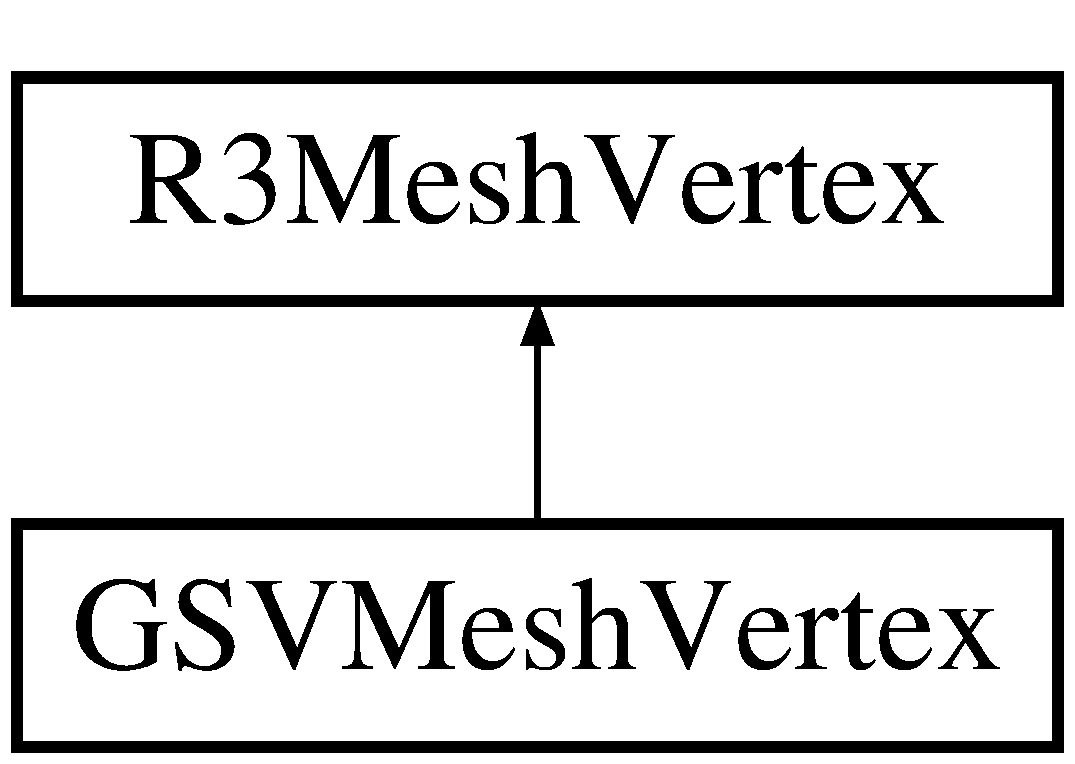
\includegraphics[height=2.000000cm]{class_r3_mesh_vertex}
\end{center}
\end{figure}
\subsection*{Protected Attributes}
\begin{DoxyCompactItemize}
\item 
\hyperlink{class_r_n_array}{R\+N\+Array}$<$ \hyperlink{class_r3_mesh_edge}{R3\+Mesh\+Edge} $\ast$ $>$ {\bfseries edges}\hypertarget{class_r3_mesh_vertex_ac82c048634a0ff8869a69ea2da8d3710}{}\label{class_r3_mesh_vertex_ac82c048634a0ff8869a69ea2da8d3710}

\item 
\hyperlink{class_r3_point}{R3\+Point} {\bfseries position}\hypertarget{class_r3_mesh_vertex_a6fa33f78f341f24a2385a874323f8a1a}{}\label{class_r3_mesh_vertex_a6fa33f78f341f24a2385a874323f8a1a}

\item 
\hyperlink{class_r3_vector}{R3\+Vector} {\bfseries normal}\hypertarget{class_r3_mesh_vertex_aa923ea74d42e30462aeb01cf34689dbe}{}\label{class_r3_mesh_vertex_aa923ea74d42e30462aeb01cf34689dbe}

\item 
\hyperlink{class_r_n_rgb}{R\+N\+Rgb} {\bfseries color}\hypertarget{class_r3_mesh_vertex_a8c7f99ac5454c989550632784ae80f43}{}\label{class_r3_mesh_vertex_a8c7f99ac5454c989550632784ae80f43}

\item 
R\+N\+Scalar {\bfseries curvature}\hypertarget{class_r3_mesh_vertex_abd8ef10ffc5c6852ae2fd7003d8577fe}{}\label{class_r3_mesh_vertex_abd8ef10ffc5c6852ae2fd7003d8577fe}

\item 
int {\bfseries id}\hypertarget{class_r3_mesh_vertex_a24abbbf6ab2a870e86132ccf689257a0}{}\label{class_r3_mesh_vertex_a24abbbf6ab2a870e86132ccf689257a0}

\item 
\hyperlink{class_r_n_flags}{R\+N\+Flags} {\bfseries flags}\hypertarget{class_r3_mesh_vertex_a5a87fbf4b32130977cff39710e2022c9}{}\label{class_r3_mesh_vertex_a5a87fbf4b32130977cff39710e2022c9}

\item 
R\+N\+Scalar {\bfseries value}\hypertarget{class_r3_mesh_vertex_a3867812487a5b646ee5bee59299a1443}{}\label{class_r3_mesh_vertex_a3867812487a5b646ee5bee59299a1443}

\item 
R\+N\+Mark {\bfseries mark}\hypertarget{class_r3_mesh_vertex_a88522dbdabe18692579ca87e38bec18f}{}\label{class_r3_mesh_vertex_a88522dbdabe18692579ca87e38bec18f}

\item 
void $\ast$ {\bfseries data}\hypertarget{class_r3_mesh_vertex_abe61d88de801bc6cbc7562dbdb032e83}{}\label{class_r3_mesh_vertex_abe61d88de801bc6cbc7562dbdb032e83}

\end{DoxyCompactItemize}
\subsection*{Friends}
\begin{DoxyCompactItemize}
\item 
class {\bfseries R3\+Mesh}\hypertarget{class_r3_mesh_vertex_ad14836d445f783f84efa263168bb3167}{}\label{class_r3_mesh_vertex_ad14836d445f783f84efa263168bb3167}

\end{DoxyCompactItemize}


The documentation for this class was generated from the following files\+:\begin{DoxyCompactItemize}
\item 
R3\+Shapes/R3\+Mesh.\+h\item 
R3\+Shapes/R3\+Mesh.\+cpp\end{DoxyCompactItemize}

\hypertarget{class_r3_model}{}\section{R3\+Model Class Reference}
\label{class_r3_model}\index{R3\+Model@{R3\+Model}}
\subsection*{Public Member Functions}
\begin{DoxyCompactItemize}
\item 
{\bfseries R3\+Model} (\hyperlink{class_r3_triangle_array}{R3\+Triangle\+Array} $\ast$triangles, const \hyperlink{class_r_n_array}{R\+N\+Array}$<$ \hyperlink{class_r3_material}{R3\+Material} $\ast$ $>$ \&materials, const \hyperlink{class_r_n_array}{R\+N\+Array}$<$ \hyperlink{class_r3_material}{R3\+Material} $\ast$ $>$ \&triangle\+\_\+materials, const \hyperlink{class_r_n_array}{R\+N\+Array}$<$ \hyperlink{class_r_n_array}{R\+N\+Array}$<$ \hyperlink{class_r3_triangle}{R3\+Triangle} $\ast$ $>$ $\ast$ $>$ \&material\+\_\+triangles)\hypertarget{class_r3_model_abea150858ccf81e2655e73589209c91a}{}\label{class_r3_model_abea150858ccf81e2655e73589209c91a}

\item 
\hyperlink{class_r3_box}{R3\+Box} {\bfseries B\+Box} (void) const \hypertarget{class_r3_model_a6e108beed66d3eb7a142af9d3460de00}{}\label{class_r3_model_a6e108beed66d3eb7a142af9d3460de00}

\item 
\hyperlink{class_r3_point}{R3\+Point} {\bfseries Centroid} (void) const \hypertarget{class_r3_model_ac4e96731fe528309a88b0e573884b434}{}\label{class_r3_model_ac4e96731fe528309a88b0e573884b434}

\item 
int {\bfseries N\+Vertices} (void) const \hypertarget{class_r3_model_a4eba4dcc6b2be06d36404d9f3597ac44}{}\label{class_r3_model_a4eba4dcc6b2be06d36404d9f3597ac44}

\item 
\hyperlink{class_r3_triangle_vertex}{R3\+Triangle\+Vertex} $\ast$ {\bfseries Vertex} (int k) const \hypertarget{class_r3_model_afe11cc852a96671bc1d1fb45f13c4c15}{}\label{class_r3_model_afe11cc852a96671bc1d1fb45f13c4c15}

\item 
int {\bfseries N\+Triangles} (void) const \hypertarget{class_r3_model_acaf55cbf171d8fae02d269d3d85619e2}{}\label{class_r3_model_acaf55cbf171d8fae02d269d3d85619e2}

\item 
\hyperlink{class_r3_triangle}{R3\+Triangle} $\ast$ {\bfseries Triangle} (int k) const \hypertarget{class_r3_model_ac71c48f63526a6878542533abcd79613}{}\label{class_r3_model_ac71c48f63526a6878542533abcd79613}

\item 
int {\bfseries N\+Materials} (void) const \hypertarget{class_r3_model_aed83008a79a44c7b76f057a77d6581da}{}\label{class_r3_model_aed83008a79a44c7b76f057a77d6581da}

\item 
\hyperlink{class_r3_material}{R3\+Material} $\ast$ {\bfseries Material} (int k) const \hypertarget{class_r3_model_a5dd87acb4921f7ddc152b4fac221be11}{}\label{class_r3_model_a5dd87acb4921f7ddc152b4fac221be11}

\item 
\hyperlink{class_r3_material}{R3\+Material} $\ast$ {\bfseries Triangle\+Material} (int triangle\+\_\+index) const \hypertarget{class_r3_model_af1233b923c3b80281b6e32fc4a6ceece}{}\label{class_r3_model_af1233b923c3b80281b6e32fc4a6ceece}

\item 
R\+N\+Boolean {\bfseries Intersects} (const \hyperlink{class_r3_ray}{R3\+Ray} \&ray, \hyperlink{class_r3_point}{R3\+Point} $\ast$hit\+\_\+point=N\+U\+LL, \hyperlink{class_r3_vector}{R3\+Vector} $\ast$hit\+\_\+normal=N\+U\+LL, R\+N\+Scalar $\ast$hit\+\_\+t=N\+U\+LL, int $\ast$hit\+\_\+triangle\+\_\+index=N\+U\+LL) const \hypertarget{class_r3_model_a999ff46636d3754a088429126a5394d1}{}\label{class_r3_model_a999ff46636d3754a088429126a5394d1}

\item 
void {\bfseries Draw} (const \hyperlink{class_r_n_flags}{R3\+Draw\+Flags} draw\+\_\+flags=R3\+\_\+\+D\+E\+F\+A\+U\+L\+T\+\_\+\+D\+R\+A\+W\+\_\+\+F\+L\+A\+GS) const \hypertarget{class_r3_model_ac1c58f0cbfee93bd8fa9be2bf1ea1432}{}\label{class_r3_model_ac1c58f0cbfee93bd8fa9be2bf1ea1432}

\item 
int {\bfseries Read\+File} (const char $\ast$filename)\hypertarget{class_r3_model_a798f1feab8d4653af2466e4cb2a53139}{}\label{class_r3_model_a798f1feab8d4653af2466e4cb2a53139}

\item 
int {\bfseries Read\+Obj\+File} (const char $\ast$filename)\hypertarget{class_r3_model_a4ee4280cd1f5077c1bfa17ef01e40da9}{}\label{class_r3_model_a4ee4280cd1f5077c1bfa17ef01e40da9}

\item 
int {\bfseries Write\+File} (const char $\ast$filename) const \hypertarget{class_r3_model_ab2b8c9ef3b145cc9c3f0aafea1e2c99b}{}\label{class_r3_model_ab2b8c9ef3b145cc9c3f0aafea1e2c99b}

\item 
int {\bfseries Write\+Obj\+File} (const char $\ast$filename) const \hypertarget{class_r3_model_a8107ccd7150a1d573aaa0fb150ed92c9}{}\label{class_r3_model_a8107ccd7150a1d573aaa0fb150ed92c9}

\end{DoxyCompactItemize}


The documentation for this class was generated from the following files\+:\begin{DoxyCompactItemize}
\item 
R3\+Graphics/R3\+Model.\+h\item 
R3\+Graphics/R3\+Model.\+cpp\end{DoxyCompactItemize}

\hypertarget{class_r3_oriented_box}{}\section{R3\+Oriented\+Box Class Reference}
\label{class_r3_oriented_box}\index{R3\+Oriented\+Box@{R3\+Oriented\+Box}}
Inheritance diagram for R3\+Oriented\+Box\+:\begin{figure}[H]
\begin{center}
\leavevmode
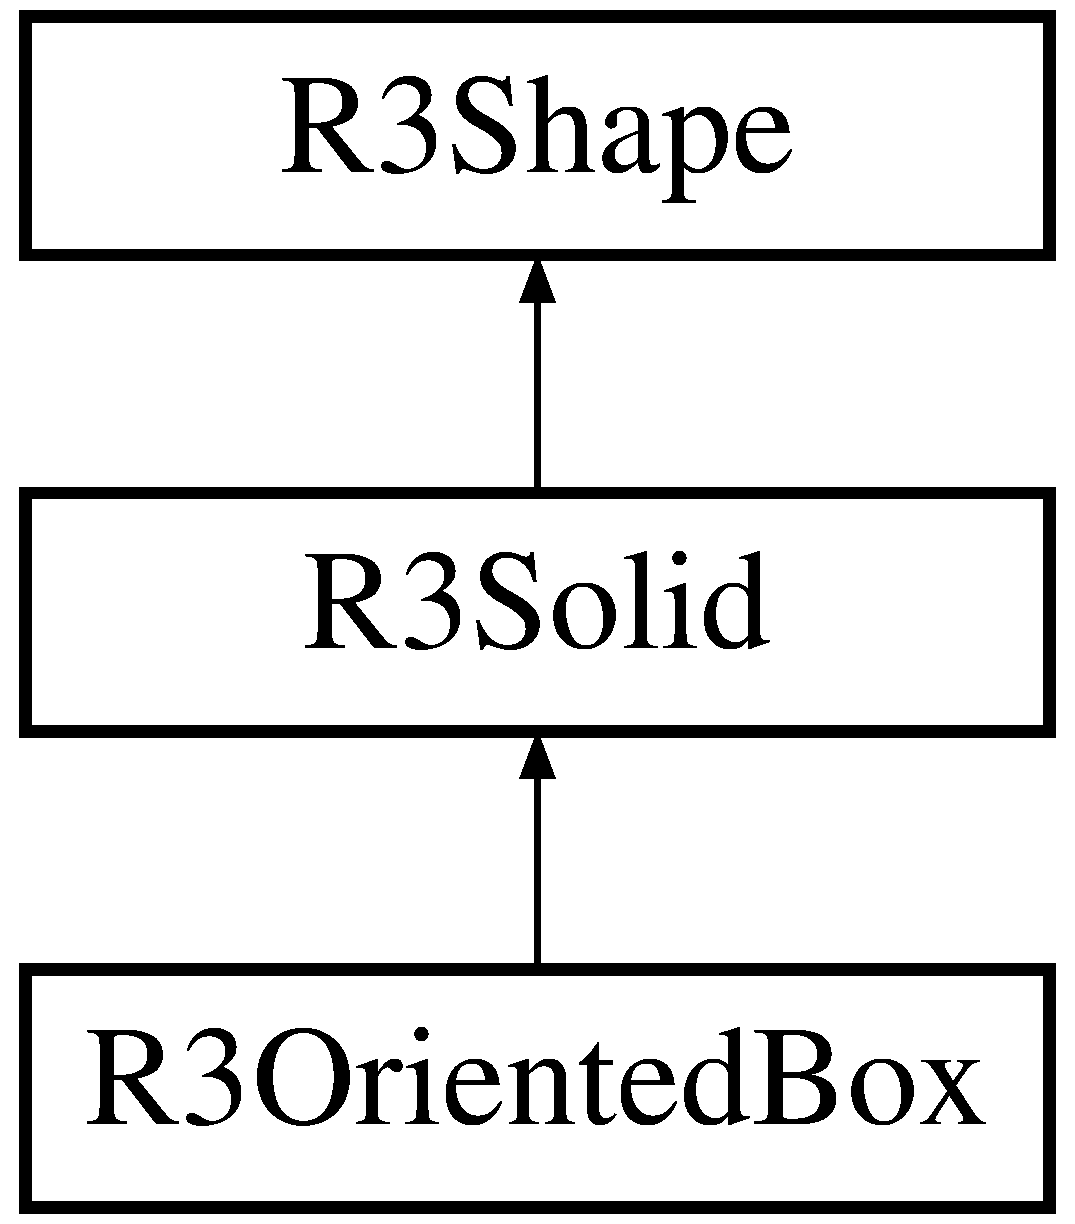
\includegraphics[height=3.000000cm]{class_r3_oriented_box}
\end{center}
\end{figure}
\subsection*{Public Member Functions}
\begin{DoxyCompactItemize}
\item 
{\bfseries R3\+Oriented\+Box} (const \hyperlink{class_r3_oriented_box}{R3\+Oriented\+Box} \&\hyperlink{structbox}{box})\hypertarget{class_r3_oriented_box_a2289e108730b037d661682cd00c52963}{}\label{class_r3_oriented_box_a2289e108730b037d661682cd00c52963}

\item 
{\bfseries R3\+Oriented\+Box} (const \hyperlink{class_r3_point}{R3\+Point} \&center, const \hyperlink{class_r3_vector}{R3\+Vector} \&axis0, const \hyperlink{class_r3_vector}{R3\+Vector} \&axis1, const \hyperlink{class_r3_vector}{R3\+Vector} \&axis2)\hypertarget{class_r3_oriented_box_a7aedb602e10faab8d73c48601cc17ad1}{}\label{class_r3_oriented_box_a7aedb602e10faab8d73c48601cc17ad1}

\item 
{\bfseries R3\+Oriented\+Box} (const \hyperlink{class_r3_point}{R3\+Point} \&center, const \hyperlink{class_r3_vector}{R3\+Vector} \&axis0, const \hyperlink{class_r3_vector}{R3\+Vector} \&axis1, R\+N\+Scalar radius0, R\+N\+Scalar radius1, R\+N\+Scalar radius2)\hypertarget{class_r3_oriented_box_a741128e4f66d74121d914d7d56d9d29a}{}\label{class_r3_oriented_box_a741128e4f66d74121d914d7d56d9d29a}

\item 
const \hyperlink{class_r3_point}{R3\+Point} \& {\bfseries Center} (void) const \hypertarget{class_r3_oriented_box_ae263d49700476287b856b59bb16922ac}{}\label{class_r3_oriented_box_ae263d49700476287b856b59bb16922ac}

\item 
const \hyperlink{class_r3_triad}{R3\+Triad} \& {\bfseries Axes} (void) const \hypertarget{class_r3_oriented_box_ae83a2a1a1bf70cbd81c64d53c00157c3}{}\label{class_r3_oriented_box_ae83a2a1a1bf70cbd81c64d53c00157c3}

\item 
const \hyperlink{class_r3_coord_system}{R3\+Coord\+System} \& {\bfseries Coord\+System} (void) const \hypertarget{class_r3_oriented_box_aa1705e61cd31720ea447e71fc4c1caf0}{}\label{class_r3_oriented_box_aa1705e61cd31720ea447e71fc4c1caf0}

\item 
const R\+N\+Length {\bfseries Min\+Radius} (void) const \hypertarget{class_r3_oriented_box_aab76939f941137e503dba9a0bae78b68}{}\label{class_r3_oriented_box_aab76939f941137e503dba9a0bae78b68}

\item 
const R\+N\+Length {\bfseries Max\+Radius} (void) const \hypertarget{class_r3_oriented_box_ad2d7be638bc52f27bc6592ad55dbe5e6}{}\label{class_r3_oriented_box_ad2d7be638bc52f27bc6592ad55dbe5e6}

\item 
const R\+N\+Length {\bfseries Diagonal\+Radius} (void) const \hypertarget{class_r3_oriented_box_ab749654a798015a22124ab60ae1599d0}{}\label{class_r3_oriented_box_ab749654a798015a22124ab60ae1599d0}

\item 
const \hyperlink{class_r3_vector}{R3\+Vector} \& {\bfseries Axis} (R\+N\+Dimension dim) const \hypertarget{class_r3_oriented_box_aadb9205a36799c7f8cb8fb307dc5206b}{}\label{class_r3_oriented_box_aadb9205a36799c7f8cb8fb307dc5206b}

\item 
const R\+N\+Length {\bfseries Radius} (R\+N\+Dimension dim) const \hypertarget{class_r3_oriented_box_ab1c602d81b7e2ad718cb8ed28019b0f0}{}\label{class_r3_oriented_box_ab1c602d81b7e2ad718cb8ed28019b0f0}

\item 
const \hyperlink{class_r3_point}{R3\+Point} {\bfseries Corner} (R\+N\+Octant octant) const \hypertarget{class_r3_oriented_box_a718fc57771ac9d97d7bcb3f04b1580e6}{}\label{class_r3_oriented_box_a718fc57771ac9d97d7bcb3f04b1580e6}

\item 
const \hyperlink{class_r3_point}{R3\+Point} {\bfseries Corner} (R\+N\+Direction dir0, R\+N\+Direction dir1, R\+N\+Direction dir2) const \hypertarget{class_r3_oriented_box_a40605c09890c36c20235681b9e7307ad}{}\label{class_r3_oriented_box_a40605c09890c36c20235681b9e7307ad}

\item 
const \hyperlink{class_r3_plane}{R3\+Plane} {\bfseries Plane} (R\+N\+Side side) const \hypertarget{class_r3_oriented_box_a520f8c9cd7ea8c58f4698c65f75184bc}{}\label{class_r3_oriented_box_a520f8c9cd7ea8c58f4698c65f75184bc}

\item 
const \hyperlink{class_r3_plane}{R3\+Plane} {\bfseries Plane} (R\+N\+Direction dir, R\+N\+Dimension dim) const \hypertarget{class_r3_oriented_box_a0e2a334dc9608a036e9a1527dd502c87}{}\label{class_r3_oriented_box_a0e2a334dc9608a036e9a1527dd502c87}

\item 
const R\+N\+Boolean {\bfseries Is\+Empty} (void) const \hypertarget{class_r3_oriented_box_abe3b32e3d68d8db3b143c96a7b6fb3dc}{}\label{class_r3_oriented_box_abe3b32e3d68d8db3b143c96a7b6fb3dc}

\item 
const R\+N\+Boolean {\bfseries Is\+Finite} (void) const \hypertarget{class_r3_oriented_box_a2cdf10094f22d8d05069a6ceef32db95}{}\label{class_r3_oriented_box_a2cdf10094f22d8d05069a6ceef32db95}

\item 
virtual const R\+N\+Boolean {\bfseries Is\+Point} (void) const \hypertarget{class_r3_oriented_box_af786c1ea59a26cb441760b3b421d2e18}{}\label{class_r3_oriented_box_af786c1ea59a26cb441760b3b421d2e18}

\item 
virtual const R\+N\+Boolean {\bfseries Is\+Linear} (void) const \hypertarget{class_r3_oriented_box_a2c2e824b7f03dda95a0b1e9926ee3936}{}\label{class_r3_oriented_box_a2c2e824b7f03dda95a0b1e9926ee3936}

\item 
virtual const R\+N\+Boolean {\bfseries Is\+Planar} (void) const \hypertarget{class_r3_oriented_box_afa802d46aae18cb47a31c62d898c179b}{}\label{class_r3_oriented_box_afa802d46aae18cb47a31c62d898c179b}

\item 
virtual const R\+N\+Boolean {\bfseries Is\+Convex} (void) const \hypertarget{class_r3_oriented_box_a28080a454bb19b053aa5df51f25939b5}{}\label{class_r3_oriented_box_a28080a454bb19b053aa5df51f25939b5}

\item 
virtual const \hyperlink{class_r_n_interval}{R\+N\+Interval} {\bfseries N\+Facets} (void) const \hypertarget{class_r3_oriented_box_ac2a0bae4aba417cc019709091f79eaa1}{}\label{class_r3_oriented_box_ac2a0bae4aba417cc019709091f79eaa1}

\item 
virtual const R\+N\+Area {\bfseries Area} (void) const \hypertarget{class_r3_oriented_box_a95f395ba15472c9b4bf9b5753b93d58f}{}\label{class_r3_oriented_box_a95f395ba15472c9b4bf9b5753b93d58f}

\item 
virtual const R\+N\+Volume {\bfseries Volume} (void) const \hypertarget{class_r3_oriented_box_a2dc460f69946df1ad89f1dd61c25a414}{}\label{class_r3_oriented_box_a2dc460f69946df1ad89f1dd61c25a414}

\item 
virtual const \hyperlink{class_r3_point}{R3\+Point} {\bfseries Centroid} (void) const \hypertarget{class_r3_oriented_box_aa73008cab4be36b8ff961548a8dc4048}{}\label{class_r3_oriented_box_aa73008cab4be36b8ff961548a8dc4048}

\item 
virtual const \hyperlink{class_r3_point}{R3\+Point} {\bfseries Closest\+Point} (const \hyperlink{class_r3_point}{R3\+Point} \&point) const \hypertarget{class_r3_oriented_box_a56d278fc5d1fc5fb329af0fcfe4ab31f}{}\label{class_r3_oriented_box_a56d278fc5d1fc5fb329af0fcfe4ab31f}

\item 
virtual const \hyperlink{class_r3_point}{R3\+Point} {\bfseries Furthest\+Point} (const \hyperlink{class_r3_point}{R3\+Point} \&point) const \hypertarget{class_r3_oriented_box_a5584bfed95d462b36bef26f30ce5d83b}{}\label{class_r3_oriented_box_a5584bfed95d462b36bef26f30ce5d83b}

\item 
virtual const \hyperlink{class_r3_shape}{R3\+Shape} \& {\bfseries B\+Shape} (void) const \hypertarget{class_r3_oriented_box_ae818d40761cc8ac0da5ae9c9a1ff3002}{}\label{class_r3_oriented_box_ae818d40761cc8ac0da5ae9c9a1ff3002}

\item 
virtual const \hyperlink{class_r3_box}{R3\+Box} {\bfseries B\+Box} (void) const \hypertarget{class_r3_oriented_box_ab2a7f8e0dfc7079d41b6f80c7efe35c3}{}\label{class_r3_oriented_box_ab2a7f8e0dfc7079d41b6f80c7efe35c3}

\item 
virtual const \hyperlink{class_r3_sphere}{R3\+Sphere} {\bfseries B\+Sphere} (void) const \hypertarget{class_r3_oriented_box_af604ff36dacf9183249d0ae3c0c36d87}{}\label{class_r3_oriented_box_af604ff36dacf9183249d0ae3c0c36d87}

\item 
virtual void {\bfseries Empty} (void)\hypertarget{class_r3_oriented_box_af5c8365a058cfa78cf7e3c062ffcd96b}{}\label{class_r3_oriented_box_af5c8365a058cfa78cf7e3c062ffcd96b}

\item 
virtual void {\bfseries Translate} (const \hyperlink{class_r3_vector}{R3\+Vector} \&vector)\hypertarget{class_r3_oriented_box_afe9cf0c09cacfbf485eb91cc3a2c3766}{}\label{class_r3_oriented_box_afe9cf0c09cacfbf485eb91cc3a2c3766}

\item 
virtual void {\bfseries Reposition} (const \hyperlink{class_r3_point}{R3\+Point} \&center)\hypertarget{class_r3_oriented_box_aeed49c7c6c2e1735e9c35672bfb06e07}{}\label{class_r3_oriented_box_aeed49c7c6c2e1735e9c35672bfb06e07}

\item 
virtual void {\bfseries Resize} (R\+N\+Length radius0, R\+N\+Length radius1, R\+N\+Length radius2)\hypertarget{class_r3_oriented_box_af6b7b6f80b4ae8ac2f9b5fc32b776175}{}\label{class_r3_oriented_box_af6b7b6f80b4ae8ac2f9b5fc32b776175}

\item 
virtual void {\bfseries Reorient} (const \hyperlink{class_r3_vector}{R3\+Vector} \&axis0, const \hyperlink{class_r3_vector}{R3\+Vector} \&axis1)\hypertarget{class_r3_oriented_box_a5692cc0b0fcace1d1e66b4df479a3d4a}{}\label{class_r3_oriented_box_a5692cc0b0fcace1d1e66b4df479a3d4a}

\item 
virtual void {\bfseries Transform} (const \hyperlink{class_r3_transformation}{R3\+Transformation} \&transformation)\hypertarget{class_r3_oriented_box_a84c3e78dd9dc204ff0627aa584e5eddf}{}\label{class_r3_oriented_box_a84c3e78dd9dc204ff0627aa584e5eddf}

\item 
virtual void {\bfseries Reset} (const \hyperlink{class_r3_point}{R3\+Point} \&center, const \hyperlink{class_r3_vector}{R3\+Vector} \&axis0, const \hyperlink{class_r3_vector}{R3\+Vector} \&axis1, R\+N\+Scalar radius0, R\+N\+Scalar radius1, R\+N\+Scalar radius2)\hypertarget{class_r3_oriented_box_aa52e70fbfd3589223610ddcfa4c1313b}{}\label{class_r3_oriented_box_aa52e70fbfd3589223610ddcfa4c1313b}

\item 
virtual void {\bfseries Draw} (const \hyperlink{class_r_n_flags}{R3\+Draw\+Flags} draw\+\_\+flags=R3\+\_\+\+D\+E\+F\+A\+U\+L\+T\+\_\+\+D\+R\+A\+W\+\_\+\+F\+L\+A\+GS) const \hypertarget{class_r3_oriented_box_a3ab43dc67d7dd7bf6aa58bdca2c9f343}{}\label{class_r3_oriented_box_a3ab43dc67d7dd7bf6aa58bdca2c9f343}

\item 
R\+N\+Boolean {\bfseries operator==} (const \hyperlink{class_r3_oriented_box}{R3\+Oriented\+Box} \&\hyperlink{structbox}{box}) const \hypertarget{class_r3_oriented_box_ae136893a8dd4b75314483e164b3eb6d9}{}\label{class_r3_oriented_box_ae136893a8dd4b75314483e164b3eb6d9}

\item 
R\+N\+Boolean {\bfseries operator!=} (const \hyperlink{class_r3_oriented_box}{R3\+Oriented\+Box} \&\hyperlink{structbox}{box}) const \hypertarget{class_r3_oriented_box_a32a4bc55b2b0d5eb7bdc043ea9adf9de}{}\label{class_r3_oriented_box_a32a4bc55b2b0d5eb7bdc043ea9adf9de}

\item 
{\bfseries R\+N\+\_\+\+C\+L\+A\+S\+S\+\_\+\+T\+Y\+P\+E\+\_\+\+D\+E\+C\+L\+A\+R\+A\+T\+I\+O\+NS} (\hyperlink{class_r3_oriented_box}{R3\+Oriented\+Box})\hypertarget{class_r3_oriented_box_a4b3849e36f419171a90522b8867a5f71}{}\label{class_r3_oriented_box_a4b3849e36f419171a90522b8867a5f71}

\item 
{\bfseries R3\+\_\+\+S\+H\+A\+P\+E\+\_\+\+R\+E\+L\+A\+T\+I\+O\+N\+S\+H\+I\+P\+\_\+\+D\+E\+C\+L\+A\+R\+A\+T\+I\+O\+NS} (\hyperlink{class_r3_oriented_box}{R3\+Oriented\+Box})\hypertarget{class_r3_oriented_box_ad47428562a81d39534ef559e21f441f3}{}\label{class_r3_oriented_box_ad47428562a81d39534ef559e21f441f3}

\end{DoxyCompactItemize}


The documentation for this class was generated from the following files\+:\begin{DoxyCompactItemize}
\item 
R3\+Shapes/R3\+Oriented\+Box.\+h\item 
R3\+Shapes/R3\+Draw.\+cpp\item 
R3\+Shapes/R3\+Oriented\+Box.\+cpp\end{DoxyCompactItemize}

\hypertarget{class_r3_planar_grid}{}\section{R3\+Planar\+Grid Class Reference}
\label{class_r3_planar_grid}\index{R3\+Planar\+Grid@{R3\+Planar\+Grid}}
\subsection*{Public Member Functions}
\begin{DoxyCompactItemize}
\item 
{\bfseries R3\+Planar\+Grid} (const \hyperlink{class_r3_plane}{R3\+Plane} \&plane, const \hyperlink{class_r3_box}{R3\+Box} \&world\+\_\+bbox, R\+N\+Length spacing)\hypertarget{class_r3_planar_grid_ac891cfdd5fcb70dc016bd8861d4db3c7}{}\label{class_r3_planar_grid_ac891cfdd5fcb70dc016bd8861d4db3c7}

\item 
{\bfseries R3\+Planar\+Grid} (const \hyperlink{class_r3_plane}{R3\+Plane} \&plane, const \hyperlink{class_r3_box}{R3\+Box} \&world\+\_\+bbox, const \hyperlink{class_r3_point}{R3\+Point} \&origin, const \hyperlink{class_r3_vector}{R3\+Vector} \&yaxis, R\+N\+Length spacing)\hypertarget{class_r3_planar_grid_a801ee5cba9c7befa12c6385be752d852}{}\label{class_r3_planar_grid_a801ee5cba9c7befa12c6385be752d852}

\item 
{\bfseries R3\+Planar\+Grid} (const \hyperlink{class_r3_plane}{R3\+Plane} \&plane, const \hyperlink{class_r3_point}{R3\+Point} \&origin, const \hyperlink{class_r3_vector}{R3\+Vector} \&yaxis, R\+N\+Length xradius, R\+N\+Length yradius, R\+N\+Length offplane\+\_\+radius, R\+N\+Length spacing)\hypertarget{class_r3_planar_grid_a2b281aa98dca77597c967d633474ab96}{}\label{class_r3_planar_grid_a2b281aa98dca77597c967d633474ab96}

\item 
int {\bfseries N\+Entries} () const \hypertarget{class_r3_planar_grid_a58be9d1568ca481b05ecdc05bd825fb5}{}\label{class_r3_planar_grid_a58be9d1568ca481b05ecdc05bd825fb5}

\item 
int {\bfseries X\+Resolution} (void) const \hypertarget{class_r3_planar_grid_a32436da37d9b148f8c105a3053e24c0d}{}\label{class_r3_planar_grid_a32436da37d9b148f8c105a3053e24c0d}

\item 
int {\bfseries Y\+Resolution} (void) const \hypertarget{class_r3_planar_grid_a8b97bbd458fb8f50c2d8fb0909bfdd84}{}\label{class_r3_planar_grid_a8b97bbd458fb8f50c2d8fb0909bfdd84}

\item 
int {\bfseries Resolution} (R\+N\+Dimension dim) const \hypertarget{class_r3_planar_grid_a7ae55662a92c049a9ee27591bae18354}{}\label{class_r3_planar_grid_a7ae55662a92c049a9ee27591bae18354}

\item 
R\+N\+Scalar {\bfseries Sum} (void) const \hypertarget{class_r3_planar_grid_a345f2c026391a1d409896a33469e2bfb}{}\label{class_r3_planar_grid_a345f2c026391a1d409896a33469e2bfb}

\item 
R\+N\+Scalar {\bfseries Mean} (void) const \hypertarget{class_r3_planar_grid_ae506719f8dc7494b18f80a4d474112a8}{}\label{class_r3_planar_grid_ae506719f8dc7494b18f80a4d474112a8}

\item 
R\+N\+Scalar {\bfseries Median} (void) const \hypertarget{class_r3_planar_grid_a55c95ac6a042f105bb27e4330276ad78}{}\label{class_r3_planar_grid_a55c95ac6a042f105bb27e4330276ad78}

\item 
R\+N\+Scalar {\bfseries Maximum} (void) const \hypertarget{class_r3_planar_grid_a0e965ac39360855436fee7dea61f896f}{}\label{class_r3_planar_grid_a0e965ac39360855436fee7dea61f896f}

\item 
R\+N\+Scalar {\bfseries Minimum} (void) const \hypertarget{class_r3_planar_grid_a92cf976f0e8702353336626668975b2b}{}\label{class_r3_planar_grid_a92cf976f0e8702353336626668975b2b}

\item 
\hyperlink{class_r_n_interval}{R\+N\+Interval} {\bfseries Range} (void) const \hypertarget{class_r3_planar_grid_ad24a0837e9cb64ba89e8d813e7cf3486}{}\label{class_r3_planar_grid_ad24a0837e9cb64ba89e8d813e7cf3486}

\item 
R\+N\+Scalar {\bfseries L1\+Norm} (void) const \hypertarget{class_r3_planar_grid_ab16e30d5e5b5aeee209972b678b8abb7}{}\label{class_r3_planar_grid_ab16e30d5e5b5aeee209972b678b8abb7}

\item 
R\+N\+Scalar {\bfseries L2\+Norm} (void) const \hypertarget{class_r3_planar_grid_a36284d7b20660163f195803df97b52f9}{}\label{class_r3_planar_grid_a36284d7b20660163f195803df97b52f9}

\item 
R\+N\+Scalar {\bfseries Area} (void) const \hypertarget{class_r3_planar_grid_ab80ed6de27e6a622ecba48838d0d2508}{}\label{class_r3_planar_grid_ab80ed6de27e6a622ecba48838d0d2508}

\item 
int {\bfseries Cardinality} (void) const \hypertarget{class_r3_planar_grid_ac371592b17e867cf92ff459a4aeb4d95}{}\label{class_r3_planar_grid_ac371592b17e867cf92ff459a4aeb4d95}

\item 
\hyperlink{class_r2_box}{R2\+Box} {\bfseries Grid\+Box} (void) const \hypertarget{class_r3_planar_grid_a25d5431fd824ddee109f8ebfd7d74c8e}{}\label{class_r3_planar_grid_a25d5431fd824ddee109f8ebfd7d74c8e}

\item 
const \hyperlink{class_r3_box}{R3\+Box} \& {\bfseries World\+Box} (void) const \hypertarget{class_r3_planar_grid_a4329a2ec1ceccb5cd4994235ffa3717a}{}\label{class_r3_planar_grid_a4329a2ec1ceccb5cd4994235ffa3717a}

\item 
const \hyperlink{class_r3_plane}{R3\+Plane} \& {\bfseries Plane} (void) const \hypertarget{class_r3_planar_grid_a4b49d4f91d2af757c352d3cc65d07e24}{}\label{class_r3_planar_grid_a4b49d4f91d2af757c352d3cc65d07e24}

\item 
const \hyperlink{class_r2_grid}{R2\+Grid} \& {\bfseries Grid} (void) const \hypertarget{class_r3_planar_grid_a967ccc311dce498fae3bb2d52dad014b}{}\label{class_r3_planar_grid_a967ccc311dce498fae3bb2d52dad014b}

\item 
R\+N\+Scalar {\bfseries Grid\+Value} (int index) const \hypertarget{class_r3_planar_grid_a54087fc611a19c5cb0b853c6605fac27}{}\label{class_r3_planar_grid_a54087fc611a19c5cb0b853c6605fac27}

\item 
R\+N\+Scalar {\bfseries Grid\+Value} (int i, int j) const \hypertarget{class_r3_planar_grid_a0fe1a3e0e1ef4b69ad4072af2321cb9d}{}\label{class_r3_planar_grid_a0fe1a3e0e1ef4b69ad4072af2321cb9d}

\item 
R\+N\+Scalar {\bfseries Grid\+Value} (R\+N\+Coord x, R\+N\+Coord y) const \hypertarget{class_r3_planar_grid_a929a65b7f69619a1418eb737745eeb62}{}\label{class_r3_planar_grid_a929a65b7f69619a1418eb737745eeb62}

\item 
R\+N\+Scalar {\bfseries Grid\+Value} (const \hyperlink{class_r2_point}{R2\+Point} \&grid\+\_\+point) const \hypertarget{class_r3_planar_grid_a4edfa20445826dca892d324ebd256fb7}{}\label{class_r3_planar_grid_a4edfa20445826dca892d324ebd256fb7}

\item 
R\+N\+Scalar {\bfseries World\+Value} (R\+N\+Coord x, R\+N\+Coord y, R\+N\+Coord z) const \hypertarget{class_r3_planar_grid_aa0ea274a0618dabef71438c0f3e4299b}{}\label{class_r3_planar_grid_aa0ea274a0618dabef71438c0f3e4299b}

\item 
R\+N\+Scalar {\bfseries World\+Value} (const \hyperlink{class_r3_point}{R3\+Point} \&world\+\_\+point) const \hypertarget{class_r3_planar_grid_abdc980c69aaf4c1c951a78787c1ae0f2}{}\label{class_r3_planar_grid_abdc980c69aaf4c1c951a78787c1ae0f2}

\item 
R\+N\+Scalar \& {\bfseries operator()} (int i, int j)\hypertarget{class_r3_planar_grid_ab52dac56807f53761e16ac1ad0f6479d}{}\label{class_r3_planar_grid_ab52dac56807f53761e16ac1ad0f6479d}

\item 
\hyperlink{class_r3_affine}{R3\+Affine} {\bfseries World\+To\+Grid\+Transformation} (void) const \hypertarget{class_r3_planar_grid_a843e44c883ed1bdef7d2c4c81d660139}{}\label{class_r3_planar_grid_a843e44c883ed1bdef7d2c4c81d660139}

\item 
\hyperlink{class_r3_affine}{R3\+Affine} {\bfseries Grid\+To\+World\+Transformation} (void) const \hypertarget{class_r3_planar_grid_a7a843d10d2c661772bb441a090cb324f}{}\label{class_r3_planar_grid_a7a843d10d2c661772bb441a090cb324f}

\item 
R\+N\+Scalar {\bfseries World\+To\+Grid\+Scale\+Factor} (void) const \hypertarget{class_r3_planar_grid_ad55ac08f098c8fb0a3faa29c9b4e03d8}{}\label{class_r3_planar_grid_ad55ac08f098c8fb0a3faa29c9b4e03d8}

\item 
R\+N\+Scalar {\bfseries Grid\+To\+World\+Scale\+Factor} (void) const \hypertarget{class_r3_planar_grid_a6a5fa18b09982fa7a02534ef4318395a}{}\label{class_r3_planar_grid_a6a5fa18b09982fa7a02534ef4318395a}

\item 
void {\bfseries Abs} (void)\hypertarget{class_r3_planar_grid_a69f5e565059b4fb7cc9ad2471f383550}{}\label{class_r3_planar_grid_a69f5e565059b4fb7cc9ad2471f383550}

\item 
void {\bfseries Sqrt} (void)\hypertarget{class_r3_planar_grid_a484cdedb4228d583d35d43fcd5274a30}{}\label{class_r3_planar_grid_a484cdedb4228d583d35d43fcd5274a30}

\item 
void {\bfseries Square} (void)\hypertarget{class_r3_planar_grid_a815f9321c006067c1545b90d815f82f8}{}\label{class_r3_planar_grid_a815f9321c006067c1545b90d815f82f8}

\item 
void {\bfseries Negate} (void)\hypertarget{class_r3_planar_grid_aa5001ad29cb2e4e1441a59b90041a933}{}\label{class_r3_planar_grid_aa5001ad29cb2e4e1441a59b90041a933}

\item 
void {\bfseries Invert} (void)\hypertarget{class_r3_planar_grid_aac275239fe21672802527218f1200387}{}\label{class_r3_planar_grid_aac275239fe21672802527218f1200387}

\item 
void {\bfseries Normalize} (void)\hypertarget{class_r3_planar_grid_a08f4c591673e7b6fb9e02e87e7998859}{}\label{class_r3_planar_grid_a08f4c591673e7b6fb9e02e87e7998859}

\item 
void {\bfseries Laplacian} (void)\hypertarget{class_r3_planar_grid_aa061f78de18e6a595950d33d74388944}{}\label{class_r3_planar_grid_aa061f78de18e6a595950d33d74388944}

\item 
void {\bfseries Laplacian} (int dim)\hypertarget{class_r3_planar_grid_aa5e7f8521ef6644378e34f406bb87385}{}\label{class_r3_planar_grid_aa5e7f8521ef6644378e34f406bb87385}

\item 
void {\bfseries Sobel} (void)\hypertarget{class_r3_planar_grid_a369ed99683974a95c06cf7adc1a99e29}{}\label{class_r3_planar_grid_a369ed99683974a95c06cf7adc1a99e29}

\item 
void {\bfseries Detect\+Edges} (void)\hypertarget{class_r3_planar_grid_a308d7fef7ba74ac9802468dde06c63d1}{}\label{class_r3_planar_grid_a308d7fef7ba74ac9802468dde06c63d1}

\item 
void {\bfseries Fill\+Holes} (void)\hypertarget{class_r3_planar_grid_ab5e40172e46b7f3658967641f16b0ecb}{}\label{class_r3_planar_grid_ab5e40172e46b7f3658967641f16b0ecb}

\item 
void {\bfseries Gradient\+Angle} (void)\hypertarget{class_r3_planar_grid_ad352325b8cbe8bcb83fe83c040d302fe}{}\label{class_r3_planar_grid_ad352325b8cbe8bcb83fe83c040d302fe}

\item 
void {\bfseries Gradient\+Magnitude} (void)\hypertarget{class_r3_planar_grid_aa1e7d0a84928ccc44ef8e3cf7905bee5}{}\label{class_r3_planar_grid_aa1e7d0a84928ccc44ef8e3cf7905bee5}

\item 
void {\bfseries Gradient} (R\+N\+Dimension dim)\hypertarget{class_r3_planar_grid_aae375faa2aca791e3c2914d96a2c1c2b}{}\label{class_r3_planar_grid_aae375faa2aca791e3c2914d96a2c1c2b}

\item 
void {\bfseries Hessian} (R\+N\+Dimension dim1, R\+N\+Dimension dim2)\hypertarget{class_r3_planar_grid_a084f099aeeb7d41e1f7b97922e7c0bdb}{}\label{class_r3_planar_grid_a084f099aeeb7d41e1f7b97922e7c0bdb}

\item 
void {\bfseries Clear} (R\+N\+Scalar value=0)\hypertarget{class_r3_planar_grid_aed82a6b6f7f1804fcbb77bd76ee12f6a}{}\label{class_r3_planar_grid_aed82a6b6f7f1804fcbb77bd76ee12f6a}

\item 
void {\bfseries Dilate} (R\+N\+Scalar grid\+\_\+distance)\hypertarget{class_r3_planar_grid_a6dcba9a3711c9540fb40bdd8ee1e0d6a}{}\label{class_r3_planar_grid_a6dcba9a3711c9540fb40bdd8ee1e0d6a}

\item 
void {\bfseries Erode} (R\+N\+Scalar grid\+\_\+distance)\hypertarget{class_r3_planar_grid_ad3cedb4477986ed6bf66863e95074d11}{}\label{class_r3_planar_grid_ad3cedb4477986ed6bf66863e95074d11}

\item 
void {\bfseries Blur} (R\+N\+Scalar grid\+\_\+sigma=2)\hypertarget{class_r3_planar_grid_a3fee6311c4ba1d98e678a405a5b6eeb2}{}\label{class_r3_planar_grid_a3fee6311c4ba1d98e678a405a5b6eeb2}

\item 
void {\bfseries Bilateral\+Filter} (R\+N\+Length grid\+\_\+sigma=2, R\+N\+Scalar value\+\_\+sigma=-\/1)\hypertarget{class_r3_planar_grid_aeb9e3acf39be9185cdda63c7bba03459}{}\label{class_r3_planar_grid_aeb9e3acf39be9185cdda63c7bba03459}

\item 
void {\bfseries Anisotropic\+Diffusion} (R\+N\+Length grid\+\_\+sigma=2, R\+N\+Scalar gradient\+\_\+sigma=-\/1)\hypertarget{class_r3_planar_grid_acc379ce25a8e25246db2b3b22e089409}{}\label{class_r3_planar_grid_acc379ce25a8e25246db2b3b22e089409}

\item 
void {\bfseries Percentile\+Filter} (R\+N\+Length grid\+\_\+radius, R\+N\+Scalar percentile)\hypertarget{class_r3_planar_grid_a73c450a54d4d0152816dd14509461d18}{}\label{class_r3_planar_grid_a73c450a54d4d0152816dd14509461d18}

\item 
void {\bfseries Min\+Filter} (R\+N\+Length grid\+\_\+radius)\hypertarget{class_r3_planar_grid_ae52410af81de7e0436f52debf78c15fe}{}\label{class_r3_planar_grid_ae52410af81de7e0436f52debf78c15fe}

\item 
void {\bfseries Max\+Filter} (R\+N\+Length grid\+\_\+radius)\hypertarget{class_r3_planar_grid_a4cea66aea6c435cc394eaa30842c377a}{}\label{class_r3_planar_grid_a4cea66aea6c435cc394eaa30842c377a}

\item 
void {\bfseries Median\+Filter} (R\+N\+Length grid\+\_\+radius)\hypertarget{class_r3_planar_grid_a0c0285eaea1580d210466c76c50890b2}{}\label{class_r3_planar_grid_a0c0285eaea1580d210466c76c50890b2}

\item 
void {\bfseries Mask\+Non\+Minima} (R\+N\+Length grid\+\_\+radius=0)\hypertarget{class_r3_planar_grid_a96004430a585c6b4657d3232fa7f50bb}{}\label{class_r3_planar_grid_a96004430a585c6b4657d3232fa7f50bb}

\item 
void {\bfseries Mask\+Non\+Maxima} (R\+N\+Length grid\+\_\+radius=0)\hypertarget{class_r3_planar_grid_a96b37e8de761174a9ed14cf457457b31}{}\label{class_r3_planar_grid_a96b37e8de761174a9ed14cf457457b31}

\item 
void {\bfseries Convolve} (const R\+N\+Scalar filter\mbox{[}3\mbox{]}\mbox{[}3\mbox{]})\hypertarget{class_r3_planar_grid_adde8a0aa7153250dc399e5f999f67808}{}\label{class_r3_planar_grid_adde8a0aa7153250dc399e5f999f67808}

\item 
void {\bfseries Substitute} (R\+N\+Scalar old\+\_\+value, R\+N\+Scalar new\+\_\+value)\hypertarget{class_r3_planar_grid_a4df52822bae9af496690a0146899332f}{}\label{class_r3_planar_grid_a4df52822bae9af496690a0146899332f}

\item 
void {\bfseries Add} (R\+N\+Scalar value)\hypertarget{class_r3_planar_grid_a0485235b93353d35afe358a39d364f74}{}\label{class_r3_planar_grid_a0485235b93353d35afe358a39d364f74}

\item 
void {\bfseries Add} (const \hyperlink{class_r3_planar_grid}{R3\+Planar\+Grid} \&grid)\hypertarget{class_r3_planar_grid_ad1e1bb238bea71e5bca04c09850a300f}{}\label{class_r3_planar_grid_ad1e1bb238bea71e5bca04c09850a300f}

\item 
void {\bfseries Subtract} (R\+N\+Scalar value)\hypertarget{class_r3_planar_grid_abbd7dfd7f265cc32d03d500899749dc8}{}\label{class_r3_planar_grid_abbd7dfd7f265cc32d03d500899749dc8}

\item 
void {\bfseries Subtract} (const \hyperlink{class_r3_planar_grid}{R3\+Planar\+Grid} \&grid)\hypertarget{class_r3_planar_grid_a9c3bab037ca2aa984a72892e770e1dd0}{}\label{class_r3_planar_grid_a9c3bab037ca2aa984a72892e770e1dd0}

\item 
void {\bfseries Multiply} (R\+N\+Scalar value)\hypertarget{class_r3_planar_grid_ac31480890a303f9a21e976c876a483c8}{}\label{class_r3_planar_grid_ac31480890a303f9a21e976c876a483c8}

\item 
void {\bfseries Multiply} (const \hyperlink{class_r3_planar_grid}{R3\+Planar\+Grid} \&grid)\hypertarget{class_r3_planar_grid_a6c1f0ae12f6b01b4bfe4e304bd187b51}{}\label{class_r3_planar_grid_a6c1f0ae12f6b01b4bfe4e304bd187b51}

\item 
void {\bfseries Divide} (R\+N\+Scalar value)\hypertarget{class_r3_planar_grid_a974aa208a17942acb139dd184c5cbfb0}{}\label{class_r3_planar_grid_a974aa208a17942acb139dd184c5cbfb0}

\item 
void {\bfseries Divide} (const \hyperlink{class_r3_planar_grid}{R3\+Planar\+Grid} \&grid)\hypertarget{class_r3_planar_grid_a97734a8df9db72f4e2298e2af003e67f}{}\label{class_r3_planar_grid_a97734a8df9db72f4e2298e2af003e67f}

\item 
void {\bfseries Pow} (R\+N\+Scalar exponent)\hypertarget{class_r3_planar_grid_ad6a68640acd74c89f46d6835d538f18b}{}\label{class_r3_planar_grid_ad6a68640acd74c89f46d6835d538f18b}

\item 
void {\bfseries Mask} (const \hyperlink{class_r3_planar_grid}{R3\+Planar\+Grid} \&grid)\hypertarget{class_r3_planar_grid_aa5f453de1dec469f89ffdbd1626b25b0}{}\label{class_r3_planar_grid_aa5f453de1dec469f89ffdbd1626b25b0}

\item 
void {\bfseries Threshold} (R\+N\+Scalar threshold, R\+N\+Scalar low, R\+N\+Scalar high)\hypertarget{class_r3_planar_grid_a7405a20260438ac2f3fafce71a21dc6a}{}\label{class_r3_planar_grid_a7405a20260438ac2f3fafce71a21dc6a}

\item 
void {\bfseries Threshold} (const \hyperlink{class_r3_planar_grid}{R3\+Planar\+Grid} \&threshold, R\+N\+Scalar low, R\+N\+Scalar high)\hypertarget{class_r3_planar_grid_a4245d8f362573d91efbe5ed4a2ca2019}{}\label{class_r3_planar_grid_a4245d8f362573d91efbe5ed4a2ca2019}

\item 
void {\bfseries Signed\+Distance\+Transform} (void)\hypertarget{class_r3_planar_grid_a2b34532fea14440043f45a7148aa814c}{}\label{class_r3_planar_grid_a2b34532fea14440043f45a7148aa814c}

\item 
void {\bfseries Squared\+Distance\+Transform} (void)\hypertarget{class_r3_planar_grid_a9c30ec7fc07f83e0923f00bf421fe51f}{}\label{class_r3_planar_grid_a9c30ec7fc07f83e0923f00bf421fe51f}

\item 
void {\bfseries Voronoi} (\hyperlink{class_r3_planar_grid}{R3\+Planar\+Grid} $\ast$squared\+\_\+distance\+\_\+grid=N\+U\+LL)\hypertarget{class_r3_planar_grid_ae3328dc279c1e2944856376c660823df}{}\label{class_r3_planar_grid_ae3328dc279c1e2944856376c660823df}

\item 
void {\bfseries Point\+Symmetry\+Transform} (int radius=-\/1)\hypertarget{class_r3_planar_grid_a2c13ab10a75c6b45d7d5f21d4f684623}{}\label{class_r3_planar_grid_a2c13ab10a75c6b45d7d5f21d4f684623}

\item 
void {\bfseries Gauss} (R\+N\+Length sigma=sqrt(8.\+0), R\+N\+Boolean square=T\+R\+UE)\hypertarget{class_r3_planar_grid_a959c686334bfa310bdd3665a370a63d1}{}\label{class_r3_planar_grid_a959c686334bfa310bdd3665a370a63d1}

\item 
void {\bfseries Resample} (int xres, int yres)\hypertarget{class_r3_planar_grid_a6c7ce352c5a9bd0c0e444646182565b6}{}\label{class_r3_planar_grid_a6c7ce352c5a9bd0c0e444646182565b6}

\item 
void {\bfseries Set\+Grid\+Value} (int index, R\+N\+Scalar value)\hypertarget{class_r3_planar_grid_ac35d0bb8e5680cb080a2a708f2dd00eb}{}\label{class_r3_planar_grid_ac35d0bb8e5680cb080a2a708f2dd00eb}

\item 
void {\bfseries Set\+Grid\+Value} (int i, int j, R\+N\+Scalar value)\hypertarget{class_r3_planar_grid_a90ce8021c6f32e3f9e53277cde1a0da5}{}\label{class_r3_planar_grid_a90ce8021c6f32e3f9e53277cde1a0da5}

\item 
void {\bfseries Add\+Grid\+Value} (int i, int j, R\+N\+Scalar value)\hypertarget{class_r3_planar_grid_a622d0f02fbf88b6a54c37c061ca7bd07}{}\label{class_r3_planar_grid_a622d0f02fbf88b6a54c37c061ca7bd07}

\item 
void {\bfseries Reset} (const \hyperlink{class_r3_plane}{R3\+Plane} \&plane, const \hyperlink{class_r3_box}{R3\+Box} \&world\+\_\+bbox, R\+N\+Length spacing)\hypertarget{class_r3_planar_grid_a6fda1eab61a3ebd3d3e921dbc5099f86}{}\label{class_r3_planar_grid_a6fda1eab61a3ebd3d3e921dbc5099f86}

\item 
void {\bfseries Reset} (const \hyperlink{class_r3_plane}{R3\+Plane} \&plane, const \hyperlink{class_r3_box}{R3\+Box} \&world\+\_\+bbox, const \hyperlink{class_r3_point}{R3\+Point} \&origin, const \hyperlink{class_r3_vector}{R3\+Vector} \&yaxis, R\+N\+Length spacing)\hypertarget{class_r3_planar_grid_ae98f076db0773002df2fc8a3f4205445}{}\label{class_r3_planar_grid_ae98f076db0773002df2fc8a3f4205445}

\item 
void {\bfseries Reset} (const \hyperlink{class_r3_plane}{R3\+Plane} \&plane, const \hyperlink{class_r3_point}{R3\+Point} \&origin, const \hyperlink{class_r3_vector}{R3\+Vector} \&yaxis, R\+N\+Length xradius, R\+N\+Length yradius, R\+N\+Length offplane\+\_\+radius, R\+N\+Length spacing)\hypertarget{class_r3_planar_grid_adedf3cfbf037cd401cf42232996f79f2}{}\label{class_r3_planar_grid_adedf3cfbf037cd401cf42232996f79f2}

\item 
void {\bfseries Rasterize\+Grid\+Point} (R\+N\+Coord x, R\+N\+Coord y, R\+N\+Scalar value)\hypertarget{class_r3_planar_grid_a125891bd35f15394b66fff4ed7e57457}{}\label{class_r3_planar_grid_a125891bd35f15394b66fff4ed7e57457}

\item 
void {\bfseries Rasterize\+World\+Point} (R\+N\+Coord x, R\+N\+Coord y, R\+N\+Coord z, R\+N\+Scalar value)\hypertarget{class_r3_planar_grid_a43cf47e1fa1b16ce8f528eaa1afa3d94}{}\label{class_r3_planar_grid_a43cf47e1fa1b16ce8f528eaa1afa3d94}

\item 
void {\bfseries Rasterize\+Grid\+Point} (const \hyperlink{class_r2_point}{R2\+Point} \&point, R\+N\+Scalar value)\hypertarget{class_r3_planar_grid_afdd4a09732386f15fa5f1bc9d23f4e94}{}\label{class_r3_planar_grid_afdd4a09732386f15fa5f1bc9d23f4e94}

\item 
void {\bfseries Rasterize\+World\+Point} (const \hyperlink{class_r3_point}{R3\+Point} \&point, R\+N\+Scalar value)\hypertarget{class_r3_planar_grid_a314704e57b482551c6ee0295b0504d48}{}\label{class_r3_planar_grid_a314704e57b482551c6ee0295b0504d48}

\item 
void {\bfseries Rasterize\+Grid\+Span} (const \hyperlink{class_r2_point}{R2\+Point} \&p1, const \hyperlink{class_r2_point}{R2\+Point} \&p2, R\+N\+Scalar value)\hypertarget{class_r3_planar_grid_a9d9cd237b3c1c3f51f7f902289111e61}{}\label{class_r3_planar_grid_a9d9cd237b3c1c3f51f7f902289111e61}

\item 
void {\bfseries Rasterize\+Grid\+Span} (const \hyperlink{class_r2_point}{R2\+Point} \&p1, const \hyperlink{class_r2_point}{R2\+Point} \&p2, R\+N\+Scalar value1, R\+N\+Scalar value2)\hypertarget{class_r3_planar_grid_a1704efc1be2a916fd80e0939a5c920de}{}\label{class_r3_planar_grid_a1704efc1be2a916fd80e0939a5c920de}

\item 
void {\bfseries Rasterize\+World\+Span} (const \hyperlink{class_r3_point}{R3\+Point} \&p1, const \hyperlink{class_r3_point}{R3\+Point} \&p2, R\+N\+Scalar value)\hypertarget{class_r3_planar_grid_ac44ddd3352aa3409e32e3755add454a6}{}\label{class_r3_planar_grid_ac44ddd3352aa3409e32e3755add454a6}

\item 
void {\bfseries Rasterize\+World\+Span} (const \hyperlink{class_r3_point}{R3\+Point} \&p1, const \hyperlink{class_r3_point}{R3\+Point} \&p2, R\+N\+Scalar value1, R\+N\+Scalar value2)\hypertarget{class_r3_planar_grid_aa3f859ac52251d80488050606043ce0c}{}\label{class_r3_planar_grid_aa3f859ac52251d80488050606043ce0c}

\item 
void {\bfseries Rasterize\+Grid\+Triangle} (const \hyperlink{class_r2_point}{R2\+Point} \&p1, const \hyperlink{class_r2_point}{R2\+Point} \&p2, const \hyperlink{class_r2_point}{R2\+Point} \&p3, R\+N\+Scalar value)\hypertarget{class_r3_planar_grid_aa0f0e716301a3853fec576372bbb9a81}{}\label{class_r3_planar_grid_aa0f0e716301a3853fec576372bbb9a81}

\item 
void {\bfseries Rasterize\+Grid\+Triangle} (const \hyperlink{class_r2_point}{R2\+Point} \&p1, const \hyperlink{class_r2_point}{R2\+Point} \&p2, const \hyperlink{class_r2_point}{R2\+Point} \&p3, R\+N\+Scalar value1, R\+N\+Scalar value2, R\+N\+Scalar value3)\hypertarget{class_r3_planar_grid_a22d3dfb2f3176f66d589a99eb029826e}{}\label{class_r3_planar_grid_a22d3dfb2f3176f66d589a99eb029826e}

\item 
void {\bfseries Rasterize\+World\+Triangle} (const \hyperlink{class_r3_point}{R3\+Point} \&p1, const \hyperlink{class_r3_point}{R3\+Point} \&p2, const \hyperlink{class_r3_point}{R3\+Point} \&p3, R\+N\+Scalar value)\hypertarget{class_r3_planar_grid_aa4755416dcd661ba27bb75e72f088948}{}\label{class_r3_planar_grid_aa4755416dcd661ba27bb75e72f088948}

\item 
void {\bfseries Rasterize\+World\+Triangle} (const \hyperlink{class_r3_point}{R3\+Point} \&p1, const \hyperlink{class_r3_point}{R3\+Point} \&p2, const \hyperlink{class_r3_point}{R3\+Point} \&p3, R\+N\+Scalar value1, R\+N\+Scalar value2, R\+N\+Scalar value3)\hypertarget{class_r3_planar_grid_a983a2462d8e5a1497642bf866ec7c307}{}\label{class_r3_planar_grid_a983a2462d8e5a1497642bf866ec7c307}

\item 
void {\bfseries Rasterize\+Grid\+Circle} (const \hyperlink{class_r2_point}{R2\+Point} \&center, R\+N\+Length radius, R\+N\+Scalar value)\hypertarget{class_r3_planar_grid_a59fc76ecbfd48c2371b40d888e311e08}{}\label{class_r3_planar_grid_a59fc76ecbfd48c2371b40d888e311e08}

\item 
void {\bfseries Rasterize\+World\+Circle} (const \hyperlink{class_r3_point}{R3\+Point} \&center, R\+N\+Length radius, R\+N\+Scalar value)\hypertarget{class_r3_planar_grid_affe8526897b9750f5181b23952fba052}{}\label{class_r3_planar_grid_affe8526897b9750f5181b23952fba052}

\item 
void {\bfseries Rasterize\+Grid\+Polygon} (const \hyperlink{class_r2_polygon}{R2\+Polygon} \&polygon, R\+N\+Scalar value)\hypertarget{class_r3_planar_grid_a91fba8c40d74cd3c0f03db9c76922255}{}\label{class_r3_planar_grid_a91fba8c40d74cd3c0f03db9c76922255}

\item 
\hyperlink{class_r3_point}{R3\+Point} {\bfseries World\+Position} (const \hyperlink{class_r2_point}{R2\+Point} \&grid\+\_\+point) const \hypertarget{class_r3_planar_grid_acfcb44622eccc585f2efa63c79a443fe}{}\label{class_r3_planar_grid_acfcb44622eccc585f2efa63c79a443fe}

\item 
\hyperlink{class_r2_point}{R2\+Point} {\bfseries Grid\+Position} (const \hyperlink{class_r3_point}{R3\+Point} \&world\+\_\+point) const \hypertarget{class_r3_planar_grid_ab5b35d3eb81aae45221a2e2b40ac8c1f}{}\label{class_r3_planar_grid_ab5b35d3eb81aae45221a2e2b40ac8c1f}

\item 
\hyperlink{class_r3_point}{R3\+Point} {\bfseries World\+Position} (R\+N\+Coord x, R\+N\+Coord y) const \hypertarget{class_r3_planar_grid_ad8e7ce309286385844c7377f1e3d846e}{}\label{class_r3_planar_grid_ad8e7ce309286385844c7377f1e3d846e}

\item 
\hyperlink{class_r2_point}{R2\+Point} {\bfseries Grid\+Position} (R\+N\+Coord x, R\+N\+Coord y, R\+N\+Coord z) const \hypertarget{class_r3_planar_grid_aade57f1c3f249916e174fe00d6460790}{}\label{class_r3_planar_grid_aade57f1c3f249916e174fe00d6460790}

\item 
int {\bfseries Read\+File} (const char $\ast$filename)\hypertarget{class_r3_planar_grid_a6cdb68aaa509c36ad4782770d7e52664}{}\label{class_r3_planar_grid_a6cdb68aaa509c36ad4782770d7e52664}

\item 
int {\bfseries Read\+Grid\+File} (const char $\ast$filename)\hypertarget{class_r3_planar_grid_a27a1a0c5e6f818466c1d845c3236fe7f}{}\label{class_r3_planar_grid_a27a1a0c5e6f818466c1d845c3236fe7f}

\item 
int {\bfseries Read\+Grid} (F\+I\+LE $\ast$fp=N\+U\+LL)\hypertarget{class_r3_planar_grid_a509da3fc4b25a39a6cf2829c2c5824f9}{}\label{class_r3_planar_grid_a509da3fc4b25a39a6cf2829c2c5824f9}

\item 
int {\bfseries Write\+File} (const char $\ast$filename) const \hypertarget{class_r3_planar_grid_a2793986f2e65b7db56d8290fca68d182}{}\label{class_r3_planar_grid_a2793986f2e65b7db56d8290fca68d182}

\item 
int {\bfseries Write\+Grid\+File} (const char $\ast$filename) const \hypertarget{class_r3_planar_grid_aa69d065d267dcfc998e2d4cb3c39c29f}{}\label{class_r3_planar_grid_aa69d065d267dcfc998e2d4cb3c39c29f}

\item 
int {\bfseries Write\+Grid} (F\+I\+LE $\ast$fp=N\+U\+LL) const \hypertarget{class_r3_planar_grid_a2aaa69a168cf64a6139d72c03421f07f}{}\label{class_r3_planar_grid_a2aaa69a168cf64a6139d72c03421f07f}

\item 
void {\bfseries Draw} (void) const \hypertarget{class_r3_planar_grid_ab52a2db40620fef9903e5f0f89609a57}{}\label{class_r3_planar_grid_ab52a2db40620fef9903e5f0f89609a57}

\item 
void {\bfseries Connected\+Component\+Label\+Filter} (R\+N\+Scalar isolevel)\hypertarget{class_r3_planar_grid_ac5ff2b0bbe8cf3c2c8de9158a78bd053}{}\label{class_r3_planar_grid_ac5ff2b0bbe8cf3c2c8de9158a78bd053}

\item 
void {\bfseries Connected\+Component\+Size\+Filter} (R\+N\+Scalar isolevel)\hypertarget{class_r3_planar_grid_a7088680684ec4ed650fcadef89f78ad1}{}\label{class_r3_planar_grid_a7088680684ec4ed650fcadef89f78ad1}

\item 
void {\bfseries Connected\+Component\+Centroid\+Filter} (R\+N\+Scalar isolevel)\hypertarget{class_r3_planar_grid_a7c45805c77150594a8f5fa404278eef8}{}\label{class_r3_planar_grid_a7c45805c77150594a8f5fa404278eef8}

\item 
void {\bfseries Connected\+Component\+Filter} (R\+N\+Scalar isolevel, R\+N\+Area min\+\_\+grid\+\_\+area, R\+N\+Area max\+\_\+grid\+\_\+area, R\+N\+Scalar under\+\_\+isolevel\+\_\+value=0, R\+N\+Scalar too\+\_\+small\+\_\+value=0, R\+N\+Scalar too\+\_\+large\+\_\+value=0)\hypertarget{class_r3_planar_grid_a62958c436997256977c3c4b7eea86fbc}{}\label{class_r3_planar_grid_a62958c436997256977c3c4b7eea86fbc}

\item 
int {\bfseries Connected\+Components} (R\+N\+Scalar isolevel=0, int max\+\_\+components=0, int $\ast$seeds=N\+U\+LL, int $\ast$sizes=N\+U\+LL, int $\ast$grid\+\_\+components=N\+U\+LL)\hypertarget{class_r3_planar_grid_a5b916d4ea4232a75309f301b0e057bce}{}\label{class_r3_planar_grid_a5b916d4ea4232a75309f301b0e057bce}

\end{DoxyCompactItemize}
\subsection*{Public Attributes}
\begin{DoxyCompactItemize}
\item 
\hyperlink{class_r3_plane}{R3\+Plane} {\bfseries plane}\hypertarget{class_r3_planar_grid_a32bde3154edefe572f7b8ab4228b1cb6}{}\label{class_r3_planar_grid_a32bde3154edefe572f7b8ab4228b1cb6}

\item 
\hyperlink{class_r3_affine}{R3\+Affine} {\bfseries transformation}\hypertarget{class_r3_planar_grid_acff82c3683e79b4ecafe66ba1fd1b2fc}{}\label{class_r3_planar_grid_acff82c3683e79b4ecafe66ba1fd1b2fc}

\item 
\hyperlink{class_r2_grid}{R2\+Grid} {\bfseries grid}\hypertarget{class_r3_planar_grid_a1208d99570cdb1ed785e00e3980b6bfa}{}\label{class_r3_planar_grid_a1208d99570cdb1ed785e00e3980b6bfa}

\item 
\hyperlink{class_r3_box}{R3\+Box} {\bfseries bbox}\hypertarget{class_r3_planar_grid_a8dacc6271b44286c13cb775d4196140b}{}\label{class_r3_planar_grid_a8dacc6271b44286c13cb775d4196140b}

\item 
int {\bfseries texture\+\_\+id}\hypertarget{class_r3_planar_grid_a1401b2f06dc1ea9c37ec5fc5dcbf5a44}{}\label{class_r3_planar_grid_a1401b2f06dc1ea9c37ec5fc5dcbf5a44}

\end{DoxyCompactItemize}


The documentation for this class was generated from the following files\+:\begin{DoxyCompactItemize}
\item 
R3\+Shapes/R3\+Planar\+Grid.\+h\item 
R3\+Shapes/R3\+Planar\+Grid.\+cpp\end{DoxyCompactItemize}

\hypertarget{class_r3_plane}{}\section{R3\+Plane Class Reference}
\label{class_r3_plane}\index{R3\+Plane@{R3\+Plane}}
\subsection*{Public Member Functions}
\begin{DoxyCompactItemize}
\item 
{\bfseries R3\+Plane} (const \hyperlink{class_r3_plane}{R3\+Plane} \&plane)\hypertarget{class_r3_plane_a0766834a9a90055513a25e57840cc107}{}\label{class_r3_plane_a0766834a9a90055513a25e57840cc107}

\item 
{\bfseries R3\+Plane} (R\+N\+Scalar a, R\+N\+Scalar b, R\+N\+Scalar c, R\+N\+Scalar d)\hypertarget{class_r3_plane_ab606e42953d1a0be357d9790378e8c59}{}\label{class_r3_plane_ab606e42953d1a0be357d9790378e8c59}

\item 
{\bfseries R3\+Plane} (const R\+N\+Scalar array\mbox{[}4\mbox{]})\hypertarget{class_r3_plane_a4c176d59f3f6aebe0e2b931544a1733b}{}\label{class_r3_plane_a4c176d59f3f6aebe0e2b931544a1733b}

\item 
{\bfseries R3\+Plane} (const \hyperlink{class_r3_vector}{R3\+Vector} \&normal, R\+N\+Scalar d)\hypertarget{class_r3_plane_aacdb37ac981b279a1f163e979f1e6c9f}{}\label{class_r3_plane_aacdb37ac981b279a1f163e979f1e6c9f}

\item 
{\bfseries R3\+Plane} (const \hyperlink{class_r3_point}{R3\+Point} \&point, const \hyperlink{class_r3_vector}{R3\+Vector} \&normal)\hypertarget{class_r3_plane_a705cb1dca4bcb9be98700096eb0c18a4}{}\label{class_r3_plane_a705cb1dca4bcb9be98700096eb0c18a4}

\item 
{\bfseries R3\+Plane} (const \hyperlink{class_r3_point}{R3\+Point} \&point, const \hyperlink{class_r3_line}{R3\+Line} \&line)\hypertarget{class_r3_plane_a05813a333c2eb072f8f0df5f9fc3f633}{}\label{class_r3_plane_a05813a333c2eb072f8f0df5f9fc3f633}

\item 
{\bfseries R3\+Plane} (const \hyperlink{class_r3_point}{R3\+Point} \&point, const \hyperlink{class_r3_vector}{R3\+Vector} \&vector1, const \hyperlink{class_r3_vector}{R3\+Vector} \&vector2)\hypertarget{class_r3_plane_a043c054a6c3700be708ae8c2835a5764}{}\label{class_r3_plane_a043c054a6c3700be708ae8c2835a5764}

\item 
{\bfseries R3\+Plane} (const \hyperlink{class_r3_point}{R3\+Point} \&point1, const \hyperlink{class_r3_point}{R3\+Point} \&point2, const \hyperlink{class_r3_point}{R3\+Point} \&point3)\hypertarget{class_r3_plane_ae3e61cce1fdb2e7a3389c261df31076e}{}\label{class_r3_plane_ae3e61cce1fdb2e7a3389c261df31076e}

\item 
{\bfseries R3\+Plane} (const \hyperlink{class_r_n_array}{R\+N\+Array}$<$ \hyperlink{class_r3_point}{R3\+Point} $\ast$ $>$ \&points, R\+N\+Boolean polygon\+\_\+vertices=T\+R\+UE)\hypertarget{class_r3_plane_a44d2356d3edbcfc3928af2b2227ea44c}{}\label{class_r3_plane_a44d2356d3edbcfc3928af2b2227ea44c}

\item 
{\bfseries R3\+Plane} (\hyperlink{class_r3_point}{R3\+Point} $\ast$points, int npoints, R\+N\+Boolean polygon\+\_\+vertices=T\+R\+UE)\hypertarget{class_r3_plane_a0eb2661363fbf9a46266b758b14347a9}{}\label{class_r3_plane_a0eb2661363fbf9a46266b758b14347a9}

\item 
const R\+N\+Scalar {\bfseries A} (void) const \hypertarget{class_r3_plane_a4aea9768246a592d03135116f0e9ff2e}{}\label{class_r3_plane_a4aea9768246a592d03135116f0e9ff2e}

\item 
const R\+N\+Scalar {\bfseries B} (void) const \hypertarget{class_r3_plane_a974857a53596fe0d4bc96a6eab4ce42e}{}\label{class_r3_plane_a974857a53596fe0d4bc96a6eab4ce42e}

\item 
const R\+N\+Scalar {\bfseries C} (void) const \hypertarget{class_r3_plane_a3a574974c6087d7ea6544b142d88f23d}{}\label{class_r3_plane_a3a574974c6087d7ea6544b142d88f23d}

\item 
const R\+N\+Scalar {\bfseries D} (void) const \hypertarget{class_r3_plane_ae9c02d14d5d8722501d0a7bc71cbaacb}{}\label{class_r3_plane_ae9c02d14d5d8722501d0a7bc71cbaacb}

\item 
const R\+N\+Scalar {\bfseries operator\mbox{[}$\,$\mbox{]}} (int i) const \hypertarget{class_r3_plane_aee92e5a0bfbdccdb3a25120685c92c2c}{}\label{class_r3_plane_aee92e5a0bfbdccdb3a25120685c92c2c}

\item 
const \hyperlink{class_r3_point}{R3\+Point} {\bfseries Point} (void) const \hypertarget{class_r3_plane_a339d225a8e0bcfb03c57ec199e3f06ee}{}\label{class_r3_plane_a339d225a8e0bcfb03c57ec199e3f06ee}

\item 
const \hyperlink{class_r3_vector}{R3\+Vector} \& {\bfseries Normal} (void) const \hypertarget{class_r3_plane_a452eb15038e7bbb158b0f867e5f3910f}{}\label{class_r3_plane_a452eb15038e7bbb158b0f867e5f3910f}

\item 
const R\+N\+Boolean {\bfseries Is\+Zero} (void) const \hypertarget{class_r3_plane_a884abb0a86507fce9ce5a686c868132d}{}\label{class_r3_plane_a884abb0a86507fce9ce5a686c868132d}

\item 
const R\+N\+Boolean {\bfseries operator==} (const \hyperlink{class_r3_plane}{R3\+Plane} \&plane) const \hypertarget{class_r3_plane_ac4bca7b2e588a10f5f9cee718c2147f1}{}\label{class_r3_plane_ac4bca7b2e588a10f5f9cee718c2147f1}

\item 
const R\+N\+Boolean {\bfseries operator!=} (const \hyperlink{class_r3_plane}{R3\+Plane} \&plane) const \hypertarget{class_r3_plane_aa07d42ab7e258bd5a2086639dc42b0f7}{}\label{class_r3_plane_aa07d42ab7e258bd5a2086639dc42b0f7}

\item 
void {\bfseries Flip} (void)\hypertarget{class_r3_plane_a399d994f1f32e5a75160b79ae4cfa0dd}{}\label{class_r3_plane_a399d994f1f32e5a75160b79ae4cfa0dd}

\item 
void {\bfseries Mirror} (const \hyperlink{class_r3_plane}{R3\+Plane} \&plane)\hypertarget{class_r3_plane_af981ff44702809575b31552b516cf2ed}{}\label{class_r3_plane_af981ff44702809575b31552b516cf2ed}

\item 
void {\bfseries Translate} (const \hyperlink{class_r3_vector}{R3\+Vector} \&vector)\hypertarget{class_r3_plane_a9238ad30b04c849208c14db912feef27}{}\label{class_r3_plane_a9238ad30b04c849208c14db912feef27}

\item 
void {\bfseries Reposition} (const \hyperlink{class_r3_point}{R3\+Point} \&point)\hypertarget{class_r3_plane_addeebe71bce54d80829059dd6ebda6ee}{}\label{class_r3_plane_addeebe71bce54d80829059dd6ebda6ee}

\item 
void {\bfseries Align} (const \hyperlink{class_r3_vector}{R3\+Vector} \&normal)\hypertarget{class_r3_plane_a71c9ed3bce285ebc0f0299c8abbfc2fc}{}\label{class_r3_plane_a71c9ed3bce285ebc0f0299c8abbfc2fc}

\item 
void {\bfseries Transform} (const \hyperlink{class_r3_transformation}{R3\+Transformation} \&transformation)\hypertarget{class_r3_plane_ad405ade9bd052aa58c35e2f8d753f525}{}\label{class_r3_plane_ad405ade9bd052aa58c35e2f8d753f525}

\item 
void {\bfseries Inverse\+Transform} (const \hyperlink{class_r3_transformation}{R3\+Transformation} \&transformation)\hypertarget{class_r3_plane_a8c65f5ad20bb21c4534cbf48697351f3}{}\label{class_r3_plane_a8c65f5ad20bb21c4534cbf48697351f3}

\item 
void {\bfseries Reset} (const \hyperlink{class_r3_point}{R3\+Point} \&point, const \hyperlink{class_r3_vector}{R3\+Vector} \&normal)\hypertarget{class_r3_plane_a066d376445cfbe638454ab258278ac76}{}\label{class_r3_plane_a066d376445cfbe638454ab258278ac76}

\item 
void {\bfseries Draw} (void) const \hypertarget{class_r3_plane_a57f20f3f11fdbd7307f593460ada9ca1}{}\label{class_r3_plane_a57f20f3f11fdbd7307f593460ada9ca1}

\item 
\hyperlink{class_r3_plane}{R3\+Plane} {\bfseries operator-\/} (void) const \hypertarget{class_r3_plane_a7836d429701695de6a12f106e56ada13}{}\label{class_r3_plane_a7836d429701695de6a12f106e56ada13}

\item 
R\+N\+Scalar \& {\bfseries operator\mbox{[}$\,$\mbox{]}} (int i)\hypertarget{class_r3_plane_a2ccc61366f9be014e4cb01db35d633bd}{}\label{class_r3_plane_a2ccc61366f9be014e4cb01db35d633bd}

\end{DoxyCompactItemize}


The documentation for this class was generated from the following files\+:\begin{DoxyCompactItemize}
\item 
R3\+Shapes/R3\+Plane.\+h\item 
R3\+Shapes/R3\+Draw.\+cpp\item 
R3\+Shapes/R3\+Plane.\+cpp\end{DoxyCompactItemize}

\hypertarget{class_r3_point}{}\section{R3\+Point Class Reference}
\label{class_r3_point}\index{R3\+Point@{R3\+Point}}
\subsection*{Public Member Functions}
\begin{DoxyCompactItemize}
\item 
{\bfseries R3\+Point} (const \hyperlink{class_r3_point}{R3\+Point} \&point)\hypertarget{class_r3_point_aeff2b2af8ead9ac23b39975e04f9617c}{}\label{class_r3_point_aeff2b2af8ead9ac23b39975e04f9617c}

\item 
{\bfseries R3\+Point} (R\+N\+Coord x, R\+N\+Coord y, R\+N\+Coord z)\hypertarget{class_r3_point_a7099143466996c64b7a8bcbd21534cf8}{}\label{class_r3_point_a7099143466996c64b7a8bcbd21534cf8}

\item 
{\bfseries R3\+Point} (const R\+N\+Coord array\mbox{[}3\mbox{]})\hypertarget{class_r3_point_a69f6257fc99a2ce28ed45bf540d8a6d0}{}\label{class_r3_point_a69f6257fc99a2ce28ed45bf540d8a6d0}

\item 
const R\+N\+Coord {\bfseries X} (void) const \hypertarget{class_r3_point_a1b8f6f4c3205423494a4552635e4272e}{}\label{class_r3_point_a1b8f6f4c3205423494a4552635e4272e}

\item 
const R\+N\+Coord {\bfseries Y} (void) const \hypertarget{class_r3_point_a43d786c38e150a4659272967df806435}{}\label{class_r3_point_a43d786c38e150a4659272967df806435}

\item 
const R\+N\+Coord {\bfseries Z} (void) const \hypertarget{class_r3_point_a98c2eb4a1bb2fc05660320dbb8c57b77}{}\label{class_r3_point_a98c2eb4a1bb2fc05660320dbb8c57b77}

\item 
const R\+N\+Coord {\bfseries Coord} (R\+N\+Dimension dim) const \hypertarget{class_r3_point_a05e0b1e436a8cd217dd3f91fb704c2f0}{}\label{class_r3_point_a05e0b1e436a8cd217dd3f91fb704c2f0}

\item 
const R\+N\+Coord {\bfseries operator\mbox{[}$\,$\mbox{]}} (R\+N\+Dimension dim) const \hypertarget{class_r3_point_ad5374304ae38adc2f8249cd490ea244b}{}\label{class_r3_point_ad5374304ae38adc2f8249cd490ea244b}

\item 
const R\+N\+Coord $\ast$ {\bfseries Coords} (void) const \hypertarget{class_r3_point_aa6986935de2cbfb65ca83c725def5925}{}\label{class_r3_point_aa6986935de2cbfb65ca83c725def5925}

\item 
const R\+N\+Boolean {\bfseries Is\+Zero} (void) const \hypertarget{class_r3_point_a688590f20a1647b6120da20182cafdea}{}\label{class_r3_point_a688590f20a1647b6120da20182cafdea}

\item 
const R\+N\+Boolean {\bfseries Is\+Finite} (void) const \hypertarget{class_r3_point_aa47adb0d0bf3e5323b409932146ef978}{}\label{class_r3_point_aa47adb0d0bf3e5323b409932146ef978}

\item 
const \hyperlink{class_r3_vector}{R3\+Vector} {\bfseries Vector} (void) const \hypertarget{class_r3_point_a3c0a7d65b83428a4c0dab3eb897105a3}{}\label{class_r3_point_a3c0a7d65b83428a4c0dab3eb897105a3}

\item 
const \hyperlink{class_r3_box}{R3\+Box} {\bfseries B\+Box} (void) const \hypertarget{class_r3_point_a798c0536f235aa335a8636507caf429f}{}\label{class_r3_point_a798c0536f235aa335a8636507caf429f}

\item 
const \hyperlink{class_r3_sphere}{R3\+Sphere} {\bfseries B\+Sphere} (void) const \hypertarget{class_r3_point_a1b00d1ff026e054ae509158150a48385}{}\label{class_r3_point_a1b00d1ff026e054ae509158150a48385}

\item 
const R\+N\+Boolean \hyperlink{class_r3_point_a5a12cb30d9490bb0e8ef66296374806c}{Collinear} (const \hyperlink{class_r3_point}{R3\+Point} \&point1, const \hyperlink{class_r3_point}{R3\+Point} \&point2) const 
\item 
const R\+N\+Boolean {\bfseries operator==} (const \hyperlink{class_r3_point}{R3\+Point} \&point) const \hypertarget{class_r3_point_a8eee023207754f118ea4bfe8181f04f1}{}\label{class_r3_point_a8eee023207754f118ea4bfe8181f04f1}

\item 
const R\+N\+Boolean {\bfseries operator!=} (const \hyperlink{class_r3_point}{R3\+Point} \&point) const \hypertarget{class_r3_point_af26dea708d773f52fcf4a34f6fa0fa79}{}\label{class_r3_point_af26dea708d773f52fcf4a34f6fa0fa79}

\item 
void {\bfseries SetX} (R\+N\+Coord x)\hypertarget{class_r3_point_abdff6c109e089cd866db215bd9a83913}{}\label{class_r3_point_abdff6c109e089cd866db215bd9a83913}

\item 
void {\bfseries SetY} (R\+N\+Coord y)\hypertarget{class_r3_point_aa2afe35e40bd115f324aa12f74972efa}{}\label{class_r3_point_aa2afe35e40bd115f324aa12f74972efa}

\item 
void {\bfseries SetZ} (R\+N\+Coord z)\hypertarget{class_r3_point_a9f4bf3bf08edd7192284535489ade7d9}{}\label{class_r3_point_a9f4bf3bf08edd7192284535489ade7d9}

\item 
void {\bfseries Set\+Coord} (R\+N\+Dimension dim, R\+N\+Coord coord)\hypertarget{class_r3_point_a944a1d08e690888bb8243a6e54a9bb0b}{}\label{class_r3_point_a944a1d08e690888bb8243a6e54a9bb0b}

\item 
void {\bfseries Translate} (const \hyperlink{class_r3_vector}{R3\+Vector} \&vector)\hypertarget{class_r3_point_a2c268a081395e787f14a93df83bbdb6d}{}\label{class_r3_point_a2c268a081395e787f14a93df83bbdb6d}

\item 
void {\bfseries Project} (const \hyperlink{class_r3_line}{R3\+Line} \&line)\hypertarget{class_r3_point_a124f2a7cd3a789b74a06c7721ed905bd}{}\label{class_r3_point_a124f2a7cd3a789b74a06c7721ed905bd}

\item 
void {\bfseries Project} (const \hyperlink{class_r3_plane}{R3\+Plane} \&plane)\hypertarget{class_r3_point_a57788221c32d35010ecf3d82422ebe90}{}\label{class_r3_point_a57788221c32d35010ecf3d82422ebe90}

\item 
void {\bfseries Mirror} (const \hyperlink{class_r3_plane}{R3\+Plane} \&plane)\hypertarget{class_r3_point_a79a572f7b95d56abf73a4c9e3c7ee74b}{}\label{class_r3_point_a79a572f7b95d56abf73a4c9e3c7ee74b}

\item 
void {\bfseries X\+Rotate} (R\+N\+Angle radians)\hypertarget{class_r3_point_a68dde7c7b99134178eee6231b148d0e0}{}\label{class_r3_point_a68dde7c7b99134178eee6231b148d0e0}

\item 
void {\bfseries Y\+Rotate} (R\+N\+Angle radians)\hypertarget{class_r3_point_ad4a834b388986a66361ca0540d81acb8}{}\label{class_r3_point_ad4a834b388986a66361ca0540d81acb8}

\item 
void {\bfseries Z\+Rotate} (R\+N\+Angle radians)\hypertarget{class_r3_point_ad6dc24e06feb116e5e322e4a34bd8b62}{}\label{class_r3_point_ad6dc24e06feb116e5e322e4a34bd8b62}

\item 
void {\bfseries Rotate} (const \hyperlink{class_r3_vector}{R3\+Vector} \&xyz\+\_\+radians)\hypertarget{class_r3_point_a739ff68aadd97d70d6f92312e041b300}{}\label{class_r3_point_a739ff68aadd97d70d6f92312e041b300}

\item 
void {\bfseries Rotate} (const \hyperlink{class_r3_quaternion}{R3\+Quaternion} \&quaternion)\hypertarget{class_r3_point_a0b871a99c6195953014af16dc5c080dc}{}\label{class_r3_point_a0b871a99c6195953014af16dc5c080dc}

\item 
void {\bfseries Rotate} (R\+N\+Axis axis, R\+N\+Angle radians)\hypertarget{class_r3_point_a726139a90f973fe779efa0263300295f}{}\label{class_r3_point_a726139a90f973fe779efa0263300295f}

\item 
void {\bfseries Rotate} (const \hyperlink{class_r3_vector}{R3\+Vector} \&axis, R\+N\+Angle theta)\hypertarget{class_r3_point_acd4501075844749aae9e4cd5b3c94c0e}{}\label{class_r3_point_acd4501075844749aae9e4cd5b3c94c0e}

\item 
void {\bfseries Rotate} (const \hyperlink{class_r3_line}{R3\+Line} \&axis, R\+N\+Angle theta)\hypertarget{class_r3_point_af63c08a8dc31279281342a1552e1504d}{}\label{class_r3_point_af63c08a8dc31279281342a1552e1504d}

\item 
void {\bfseries Transform} (const \hyperlink{class_r3_transformation}{R3\+Transformation} \&transformation)\hypertarget{class_r3_point_ae4dac4ed21c59ef1bc606d0f8e852456}{}\label{class_r3_point_ae4dac4ed21c59ef1bc606d0f8e852456}

\item 
void {\bfseries Inverse\+Transform} (const \hyperlink{class_r3_transformation}{R3\+Transformation} \&transformation)\hypertarget{class_r3_point_a64811762851c6d270ce43327f4c8228a}{}\label{class_r3_point_a64811762851c6d270ce43327f4c8228a}

\item 
void {\bfseries Reset} (R\+N\+Coord x, R\+N\+Coord y, R\+N\+Coord z)\hypertarget{class_r3_point_afa30ad6e664ef97b987af713c6ab4b7e}{}\label{class_r3_point_afa30ad6e664ef97b987af713c6ab4b7e}

\item 
void {\bfseries Draw} (void) const \hypertarget{class_r3_point_af91562573df24e58cf67c0ebe226156f}{}\label{class_r3_point_af91562573df24e58cf67c0ebe226156f}

\item 
\hyperlink{class_r3_point}{R3\+Point} \& {\bfseries operator=} (const \hyperlink{class_r3_point}{R3\+Point} \&point)\hypertarget{class_r3_point_ac30c085bfa89e10bdcdfa1bc64d7dda4}{}\label{class_r3_point_ac30c085bfa89e10bdcdfa1bc64d7dda4}

\item 
\hyperlink{class_r3_point}{R3\+Point} \& {\bfseries operator+=} (const \hyperlink{class_r3_point}{R3\+Point} \&point)\hypertarget{class_r3_point_ae1712f1eb6f5780f5241435142f572c5}{}\label{class_r3_point_ae1712f1eb6f5780f5241435142f572c5}

\item 
\hyperlink{class_r3_point}{R3\+Point} \& {\bfseries operator+=} (const \hyperlink{class_r3_vector}{R3\+Vector} \&vector)\hypertarget{class_r3_point_a4f0142ea39e215a275319d4f53b0f69c}{}\label{class_r3_point_a4f0142ea39e215a275319d4f53b0f69c}

\item 
\hyperlink{class_r3_point}{R3\+Point} \& {\bfseries operator-\/=} (const \hyperlink{class_r3_vector}{R3\+Vector} \&vector)\hypertarget{class_r3_point_a4408ecc328806ebaedcc8bd67417edcc}{}\label{class_r3_point_a4408ecc328806ebaedcc8bd67417edcc}

\item 
\hyperlink{class_r3_point}{R3\+Point} \& {\bfseries operator$\ast$=} (const R\+N\+Scalar a)\hypertarget{class_r3_point_a22c7bc9ef26edc4f8f36338f38d173d1}{}\label{class_r3_point_a22c7bc9ef26edc4f8f36338f38d173d1}

\item 
\hyperlink{class_r3_point}{R3\+Point} \& {\bfseries operator/=} (const R\+N\+Scalar a)\hypertarget{class_r3_point_ae2eb57d09b61bf1f805ddbf47bc57181}{}\label{class_r3_point_ae2eb57d09b61bf1f805ddbf47bc57181}

\item 
R\+N\+Coord \& {\bfseries operator\mbox{[}$\,$\mbox{]}} (R\+N\+Dimension dim)\hypertarget{class_r3_point_ac309f5d823e0951f50531b35757cd42f}{}\label{class_r3_point_ac309f5d823e0951f50531b35757cd42f}

\end{DoxyCompactItemize}
\subsection*{Friends}
\begin{DoxyCompactItemize}
\item 
\hyperlink{class_r3_point}{R3\+Point} {\bfseries operator-\/} (const \hyperlink{class_r3_point}{R3\+Point} \&point)\hypertarget{class_r3_point_a2b9b2cd86f7ab7e0df974d89ad0c0f15}{}\label{class_r3_point_a2b9b2cd86f7ab7e0df974d89ad0c0f15}

\item 
\hyperlink{class_r3_point}{R3\+Point} {\bfseries operator+} (const \hyperlink{class_r3_point}{R3\+Point} \&point1, const \hyperlink{class_r3_point}{R3\+Point} \&point2)\hypertarget{class_r3_point_aca79abb3dc284337df28b0a0b47b4d4a}{}\label{class_r3_point_aca79abb3dc284337df28b0a0b47b4d4a}

\item 
\hyperlink{class_r3_point}{R3\+Point} {\bfseries operator+} (const \hyperlink{class_r3_point}{R3\+Point} \&point, const \hyperlink{class_r3_vector}{R3\+Vector} \&vector)\hypertarget{class_r3_point_a395bf315cbac0a603151eb78eee9b2fa}{}\label{class_r3_point_a395bf315cbac0a603151eb78eee9b2fa}

\item 
\hyperlink{class_r3_point}{R3\+Point} {\bfseries operator+} (const \hyperlink{class_r3_vector}{R3\+Vector} \&vector, const \hyperlink{class_r3_point}{R3\+Point} \&point)\hypertarget{class_r3_point_a849673eaf1e2a90cae0afdc9d3d0e0b4}{}\label{class_r3_point_a849673eaf1e2a90cae0afdc9d3d0e0b4}

\item 
\hyperlink{class_r3_vector}{R3\+Vector} {\bfseries operator-\/} (const \hyperlink{class_r3_point}{R3\+Point} \&point1, const \hyperlink{class_r3_point}{R3\+Point} \&point2)\hypertarget{class_r3_point_a5c534d1f3962c2e70d7be72b36d5ea03}{}\label{class_r3_point_a5c534d1f3962c2e70d7be72b36d5ea03}

\item 
\hyperlink{class_r3_point}{R3\+Point} {\bfseries operator-\/} (const \hyperlink{class_r3_point}{R3\+Point} \&point, const \hyperlink{class_r3_vector}{R3\+Vector} \&vector)\hypertarget{class_r3_point_a10c15f23f6ad0fb37ba8e8a0ed95b139}{}\label{class_r3_point_a10c15f23f6ad0fb37ba8e8a0ed95b139}

\item 
\hyperlink{class_r3_point}{R3\+Point} {\bfseries operator$\ast$} (const \hyperlink{class_r3_point}{R3\+Point} \&point, const R\+N\+Scalar a)\hypertarget{class_r3_point_add54f903121b620f7aef312a92ef080f}{}\label{class_r3_point_add54f903121b620f7aef312a92ef080f}

\item 
\hyperlink{class_r3_point}{R3\+Point} {\bfseries operator$\ast$} (const R\+N\+Scalar a, const \hyperlink{class_r3_point}{R3\+Point} \&point)\hypertarget{class_r3_point_a153210287400e334fe23ff1741eb9913}{}\label{class_r3_point_a153210287400e334fe23ff1741eb9913}

\item 
\hyperlink{class_r3_point}{R3\+Point} {\bfseries operator/} (const \hyperlink{class_r3_point}{R3\+Point} \&point, const R\+N\+Scalar a)\hypertarget{class_r3_point_a16d4f82f27af9b9323f2e7eee8553c7b}{}\label{class_r3_point_a16d4f82f27af9b9323f2e7eee8553c7b}

\end{DoxyCompactItemize}


\subsection{Member Function Documentation}
\index{R3\+Point@{R3\+Point}!Collinear@{Collinear}}
\index{Collinear@{Collinear}!R3\+Point@{R3\+Point}}
\subsubsection[{\texorpdfstring{Collinear(const R3\+Point \&point1, const R3\+Point \&point2) const }{Collinear(const R3Point &point1, const R3Point &point2) const }}]{\setlength{\rightskip}{0pt plus 5cm}const R\+N\+Boolean R3\+Point\+::\+Collinear (
\begin{DoxyParamCaption}
\item[{const {\bf R3\+Point} \&}]{point1, }
\item[{const {\bf R3\+Point} \&}]{point2}
\end{DoxyParamCaption}
) const}\hypertarget{class_r3_point_a5a12cb30d9490bb0e8ef66296374806c}{}\label{class_r3_point_a5a12cb30d9490bb0e8ef66296374806c}
Check if three points are collinear 

The documentation for this class was generated from the following files\+:\begin{DoxyCompactItemize}
\item 
R3\+Shapes/R3\+Point.\+h\item 
R3\+Shapes/R3\+Draw.\+cpp\item 
R3\+Shapes/R3\+Point.\+cpp\end{DoxyCompactItemize}

\hypertarget{class_r3_point_light}{}\section{R3\+Point\+Light Class Reference}
\label{class_r3_point_light}\index{R3\+Point\+Light@{R3\+Point\+Light}}
Inheritance diagram for R3\+Point\+Light\+:\begin{figure}[H]
\begin{center}
\leavevmode
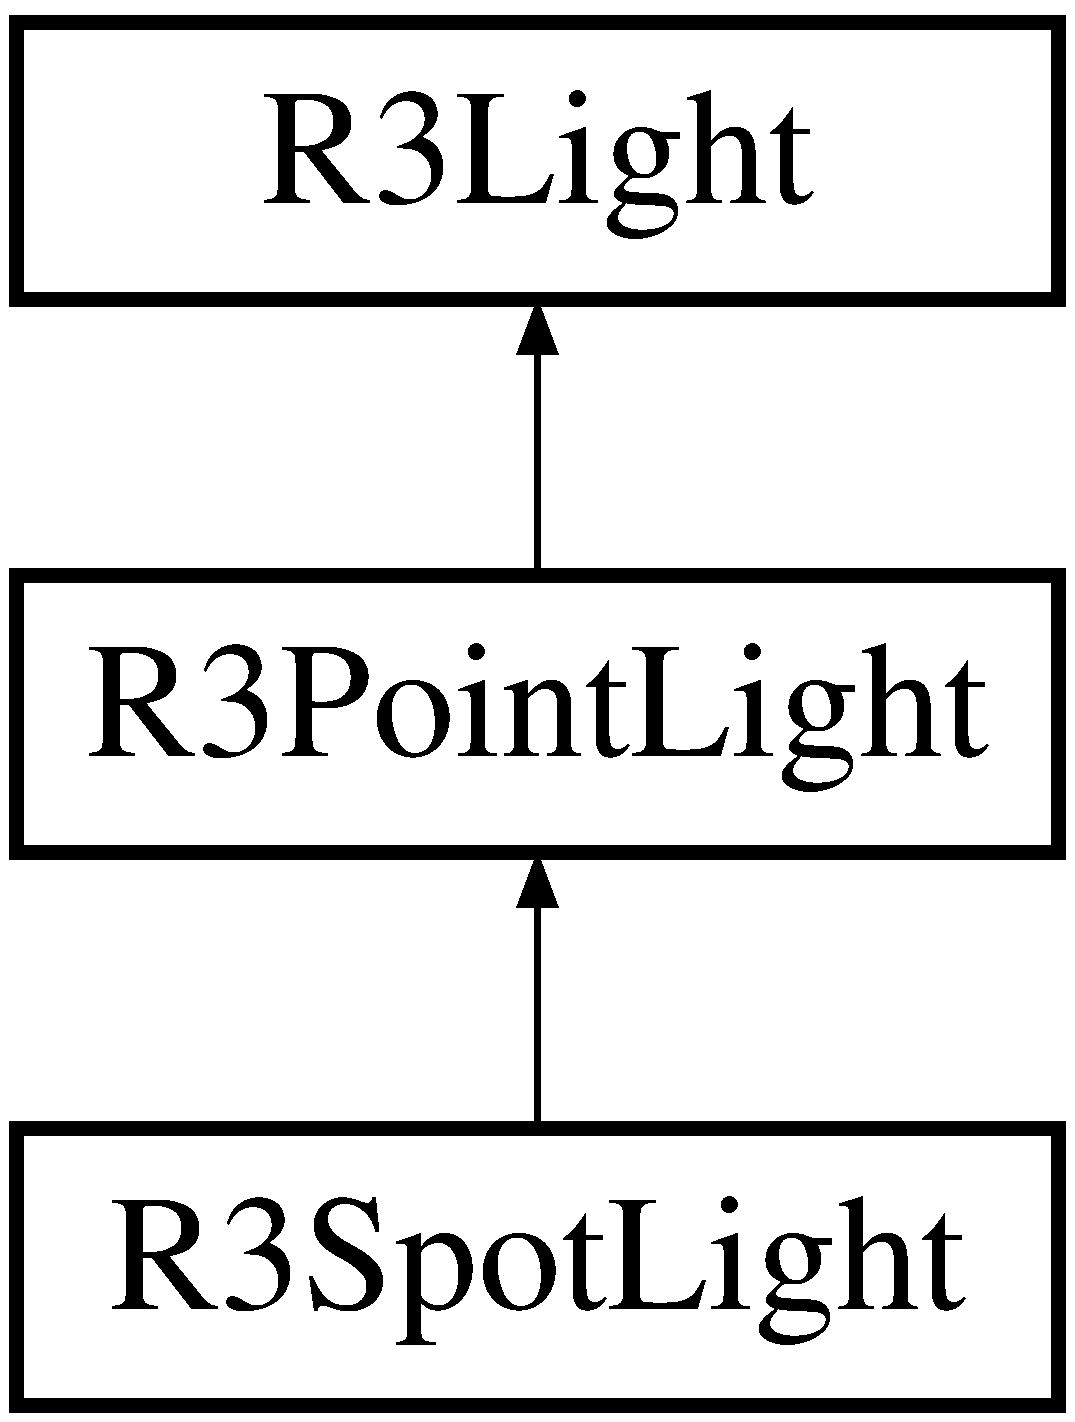
\includegraphics[height=3.000000cm]{class_r3_point_light}
\end{center}
\end{figure}
\subsection*{Public Member Functions}
\begin{DoxyCompactItemize}
\item 
{\bfseries R3\+Point\+Light} (const \hyperlink{class_r3_point_light}{R3\+Point\+Light} \&light)\hypertarget{class_r3_point_light_a8c00c92ac2bc7675332659b5f7b021fb}{}\label{class_r3_point_light_a8c00c92ac2bc7675332659b5f7b021fb}

\item 
{\bfseries R3\+Point\+Light} (const \hyperlink{class_r3_point}{R3\+Point} \&position, const \hyperlink{class_r_n_rgb}{R\+N\+Rgb} \&color, R\+N\+Scalar intensity=1.\+0, R\+N\+Boolean active=T\+R\+UE, R\+N\+Scalar ca=0, R\+N\+Scalar la=0, R\+N\+Scalar qa=1)\hypertarget{class_r3_point_light_a843f6ecd1e8b072d27d53d28aea64ae0}{}\label{class_r3_point_light_a843f6ecd1e8b072d27d53d28aea64ae0}

\item 
const \hyperlink{class_r3_point}{R3\+Point} \& {\bfseries Position} (void) const \hypertarget{class_r3_point_light_a925bc8bff38aa48523fd290705144e6e}{}\label{class_r3_point_light_a925bc8bff38aa48523fd290705144e6e}

\item 
const R\+N\+Scalar {\bfseries Constant\+Attenuation} (void) const \hypertarget{class_r3_point_light_a5f8db531141372060935b04c1ae5d0c4}{}\label{class_r3_point_light_a5f8db531141372060935b04c1ae5d0c4}

\item 
const R\+N\+Scalar {\bfseries Linear\+Attenuation} (void) const \hypertarget{class_r3_point_light_a45e645b0d3fcc666f8fd52babed73203}{}\label{class_r3_point_light_a45e645b0d3fcc666f8fd52babed73203}

\item 
const R\+N\+Scalar {\bfseries Quadratic\+Attenuation} (void) const \hypertarget{class_r3_point_light_a77e2843354808cf08bf1acb8dac41f12}{}\label{class_r3_point_light_a77e2843354808cf08bf1acb8dac41f12}

\item 
virtual void {\bfseries Set\+Position} (const \hyperlink{class_r3_point}{R3\+Point} \&position)\hypertarget{class_r3_point_light_acfcc2477fe698f54c393e16006663eaa}{}\label{class_r3_point_light_acfcc2477fe698f54c393e16006663eaa}

\item 
virtual void {\bfseries Set\+Constant\+Attenuation} (R\+N\+Scalar ca)\hypertarget{class_r3_point_light_ac202e633a3c19aa721c6391a38fede38}{}\label{class_r3_point_light_ac202e633a3c19aa721c6391a38fede38}

\item 
virtual void {\bfseries Set\+Linear\+Attenuation} (R\+N\+Scalar la)\hypertarget{class_r3_point_light_ac6f28901991aadd32b56224734de5835}{}\label{class_r3_point_light_ac6f28901991aadd32b56224734de5835}

\item 
virtual void {\bfseries Set\+Quadratic\+Attenuation} (R\+N\+Scalar qa)\hypertarget{class_r3_point_light_a826edcfc0b868922de4921feee592629}{}\label{class_r3_point_light_a826edcfc0b868922de4921feee592629}

\item 
virtual R\+N\+Scalar {\bfseries Intensity\+At\+Point} (const \hyperlink{class_r3_point}{R3\+Point} \&point) const \hypertarget{class_r3_point_light_a6192631ce7d497e7bb9f47ff94d32279}{}\label{class_r3_point_light_a6192631ce7d497e7bb9f47ff94d32279}

\item 
virtual \hyperlink{class_r3_vector}{R3\+Vector} {\bfseries Direction\+From\+Point} (const \hyperlink{class_r3_point}{R3\+Point} \&point) const \hypertarget{class_r3_point_light_a3d6a7dd4d1ff4e3d3907fd267808d4bf}{}\label{class_r3_point_light_a3d6a7dd4d1ff4e3d3907fd267808d4bf}

\item 
virtual R\+N\+Scalar {\bfseries Radius\+Of\+Influence} (R\+N\+Scalar intensity) const \hypertarget{class_r3_point_light_a77f111accced801ce2f3ce09c0f8f3b3}{}\label{class_r3_point_light_a77f111accced801ce2f3ce09c0f8f3b3}

\item 
virtual \hyperlink{class_r3_sphere}{R3\+Sphere} {\bfseries Sphere\+Of\+Influence} (R\+N\+Scalar intensity) const \hypertarget{class_r3_point_light_a3a317c0744ebd5409c1a5215a733ef21}{}\label{class_r3_point_light_a3a317c0744ebd5409c1a5215a733ef21}

\item 
virtual \hyperlink{class_r_n_rgb}{R\+N\+Rgb} {\bfseries Reflection} (const \hyperlink{class_r3_brdf}{R3\+Brdf} \&brdf, const \hyperlink{class_r3_point}{R3\+Point} \&eye, const \hyperlink{class_r3_point}{R3\+Point} \&point, const \hyperlink{class_r3_vector}{R3\+Vector} \&normal) const \hypertarget{class_r3_point_light_a0f90f489b782654f053214f8fc410ac7}{}\label{class_r3_point_light_a0f90f489b782654f053214f8fc410ac7}

\item 
virtual \hyperlink{class_r_n_rgb}{R\+N\+Rgb} {\bfseries Diffuse\+Reflection} (const \hyperlink{class_r3_brdf}{R3\+Brdf} \&brdf, const \hyperlink{class_r3_point}{R3\+Point} \&point, const \hyperlink{class_r3_vector}{R3\+Vector} \&normal) const \hypertarget{class_r3_point_light_a801ded380a187411e60a2cfa1f81e401}{}\label{class_r3_point_light_a801ded380a187411e60a2cfa1f81e401}

\item 
virtual \hyperlink{class_r_n_rgb}{R\+N\+Rgb} {\bfseries Specular\+Reflection} (const \hyperlink{class_r3_brdf}{R3\+Brdf} \&brdf, const \hyperlink{class_r3_point}{R3\+Point} \&eye, const \hyperlink{class_r3_point}{R3\+Point} \&point, const \hyperlink{class_r3_vector}{R3\+Vector} \&normal) const \hypertarget{class_r3_point_light_a1161e3aee7a77b3b159a9d4a408bf624}{}\label{class_r3_point_light_a1161e3aee7a77b3b159a9d4a408bf624}

\item 
virtual void {\bfseries Draw} (int i) const \hypertarget{class_r3_point_light_a448f51b59539733cd8e0d3e69ae2ffaf}{}\label{class_r3_point_light_a448f51b59539733cd8e0d3e69ae2ffaf}

\item 
{\bfseries R\+N\+\_\+\+C\+L\+A\+S\+S\+\_\+\+T\+Y\+P\+E\+\_\+\+D\+E\+C\+L\+A\+R\+A\+T\+I\+O\+NS} (\hyperlink{class_r3_point_light}{R3\+Point\+Light})\hypertarget{class_r3_point_light_a6a253c888dfd0716716e71cec0b4f4e1}{}\label{class_r3_point_light_a6a253c888dfd0716716e71cec0b4f4e1}

\end{DoxyCompactItemize}


The documentation for this class was generated from the following files\+:\begin{DoxyCompactItemize}
\item 
R3\+Graphics/R3\+Point\+Light.\+h\item 
R3\+Graphics/R3\+Point\+Light.\+cpp\end{DoxyCompactItemize}

\hypertarget{class_r3_quaternion}{}\section{R3\+Quaternion Class Reference}
\label{class_r3_quaternion}\index{R3\+Quaternion@{R3\+Quaternion}}
\subsection*{Public Member Functions}
\begin{DoxyCompactItemize}
\item 
{\bfseries R3\+Quaternion} (const \hyperlink{class_r3_quaternion}{R3\+Quaternion} \&quaternion)\hypertarget{class_r3_quaternion_aec672473f45d7e942e17eba9fb591733}{}\label{class_r3_quaternion_aec672473f45d7e942e17eba9fb591733}

\item 
{\bfseries R3\+Quaternion} (R\+N\+Scalar a, R\+N\+Scalar b, R\+N\+Scalar c, R\+N\+Scalar d)\hypertarget{class_r3_quaternion_a27d3b526b8b6c4033290bb87ed2327ce}{}\label{class_r3_quaternion_a27d3b526b8b6c4033290bb87ed2327ce}

\item 
{\bfseries R3\+Quaternion} (const \hyperlink{class_r3_quaternion}{R3\+Quaternion} \&quaternion1, const \hyperlink{class_r3_quaternion}{R3\+Quaternion} \&quaternion2, R\+N\+Scalar t)\hypertarget{class_r3_quaternion_a83e4338050f07d4d53b150adaabfbb32}{}\label{class_r3_quaternion_a83e4338050f07d4d53b150adaabfbb32}

\item 
{\bfseries R3\+Quaternion} (const \hyperlink{class_r3_vector}{R3\+Vector} \&axis, R\+N\+Angle theta)\hypertarget{class_r3_quaternion_a9ac4421ac87be4a51db57f49965c29b2}{}\label{class_r3_quaternion_a9ac4421ac87be4a51db57f49965c29b2}

\item 
{\bfseries R3\+Quaternion} (const \hyperlink{class_r4_matrix}{R4\+Matrix} \&matrix, int dummy)\hypertarget{class_r3_quaternion_a5e46b1e3cdf52606cd45744824b733cc}{}\label{class_r3_quaternion_a5e46b1e3cdf52606cd45744824b733cc}

\item 
{\bfseries R3\+Quaternion} (int dimension, R\+N\+Angle theta)\hypertarget{class_r3_quaternion_a5fdf5fba967c70e89a78cd5be3e11526}{}\label{class_r3_quaternion_a5fdf5fba967c70e89a78cd5be3e11526}

\item 
{\bfseries R3\+Quaternion} (R\+N\+Angle pitch, R\+N\+Angle yaw, R\+N\+Angle roll)\hypertarget{class_r3_quaternion_a71cd579b88f35c245583dda32a8ecf1c}{}\label{class_r3_quaternion_a71cd579b88f35c245583dda32a8ecf1c}

\item 
{\bfseries R3\+Quaternion} (const R\+N\+Scalar array\mbox{[}4\mbox{]})\hypertarget{class_r3_quaternion_a3c10c98b699654c1ee347b32393a5748}{}\label{class_r3_quaternion_a3c10c98b699654c1ee347b32393a5748}

\item 
const R\+N\+Scalar {\bfseries A} (void) const \hypertarget{class_r3_quaternion_a11495e24824efbb04f306e8ce7d0e8a7}{}\label{class_r3_quaternion_a11495e24824efbb04f306e8ce7d0e8a7}

\item 
const R\+N\+Scalar {\bfseries B} (void) const \hypertarget{class_r3_quaternion_a778918e12637a91b82269334259d46b1}{}\label{class_r3_quaternion_a778918e12637a91b82269334259d46b1}

\item 
const R\+N\+Scalar {\bfseries C} (void) const \hypertarget{class_r3_quaternion_a120edf9e9849ee1ad3ee91e24b691980}{}\label{class_r3_quaternion_a120edf9e9849ee1ad3ee91e24b691980}

\item 
const R\+N\+Scalar {\bfseries D} (void) const \hypertarget{class_r3_quaternion_afa927e4c5b36cfb8e0770e8d02d22b92}{}\label{class_r3_quaternion_afa927e4c5b36cfb8e0770e8d02d22b92}

\item 
const R\+N\+Scalar {\bfseries operator\mbox{[}$\,$\mbox{]}} (int i) const \hypertarget{class_r3_quaternion_a376ae66ec4afc5d53dbc2ad6ad90c767}{}\label{class_r3_quaternion_a376ae66ec4afc5d53dbc2ad6ad90c767}

\item 
const R\+N\+Boolean {\bfseries Is\+Zero} (void) const \hypertarget{class_r3_quaternion_ae22c42cc8e198acaa6be2bb08c06284c}{}\label{class_r3_quaternion_ae22c42cc8e198acaa6be2bb08c06284c}

\item 
const \hyperlink{class_r3_vector}{R3\+Vector} {\bfseries Axis} (void) const \hypertarget{class_r3_quaternion_af74cc2cc25e2c0af9b84a3b621ca5c4f}{}\label{class_r3_quaternion_af74cc2cc25e2c0af9b84a3b621ca5c4f}

\item 
const R\+N\+Angle {\bfseries Angle} (void) const \hypertarget{class_r3_quaternion_a726b45812aff9b905b30235395935800}{}\label{class_r3_quaternion_a726b45812aff9b905b30235395935800}

\item 
const \hyperlink{class_r4_matrix}{R4\+Matrix} {\bfseries Matrix} (void) const \hypertarget{class_r3_quaternion_af934573b6fc4a7391f414f9fa2f3eefb}{}\label{class_r3_quaternion_af934573b6fc4a7391f414f9fa2f3eefb}

\item 
const \hyperlink{class_r3_quaternion}{R3\+Quaternion} {\bfseries Inverse} (void) const \hypertarget{class_r3_quaternion_a541db26f54e63606ac6e166c7141ac30}{}\label{class_r3_quaternion_a541db26f54e63606ac6e166c7141ac30}

\item 
const R\+N\+Boolean {\bfseries operator==} (const \hyperlink{class_r3_quaternion}{R3\+Quaternion} \&quaternion) const \hypertarget{class_r3_quaternion_a1864313908761dd336c1fcc0946b4f32}{}\label{class_r3_quaternion_a1864313908761dd336c1fcc0946b4f32}

\item 
const R\+N\+Boolean {\bfseries operator!=} (const \hyperlink{class_r3_quaternion}{R3\+Quaternion} \&quaternion) const \hypertarget{class_r3_quaternion_a900b3664dd02655ce7dfabcd9a5e0a79}{}\label{class_r3_quaternion_a900b3664dd02655ce7dfabcd9a5e0a79}

\item 
void {\bfseries Flip} (void)\hypertarget{class_r3_quaternion_a3eec62818c63ac0216a6388b145b85c0}{}\label{class_r3_quaternion_a3eec62818c63ac0216a6388b145b85c0}

\item 
void {\bfseries Multiply} (const \hyperlink{class_r3_quaternion}{R3\+Quaternion} \&quaternion)\hypertarget{class_r3_quaternion_aabcd693be0383364af44229a281154c7}{}\label{class_r3_quaternion_aabcd693be0383364af44229a281154c7}

\item 
void {\bfseries X\+Rotate} (R\+N\+Angle radians)\hypertarget{class_r3_quaternion_a3e931dab99239131306229af06672e53}{}\label{class_r3_quaternion_a3e931dab99239131306229af06672e53}

\item 
void {\bfseries Y\+Rotate} (R\+N\+Angle radians)\hypertarget{class_r3_quaternion_af5af822a035563eaaf2bda3309889967}{}\label{class_r3_quaternion_af5af822a035563eaaf2bda3309889967}

\item 
void {\bfseries Z\+Rotate} (R\+N\+Angle radians)\hypertarget{class_r3_quaternion_a085bfc18844112f2c6910af2c112aed8}{}\label{class_r3_quaternion_a085bfc18844112f2c6910af2c112aed8}

\item 
void {\bfseries Rotate} (const \hyperlink{class_r3_vector}{R3\+Vector} \&xyz\+\_\+radians)\hypertarget{class_r3_quaternion_a8b09253e5dcff3ccc36b4251a52bdaa6}{}\label{class_r3_quaternion_a8b09253e5dcff3ccc36b4251a52bdaa6}

\item 
void {\bfseries Rotate} (int dimension, R\+N\+Angle radians)\hypertarget{class_r3_quaternion_af8153bf646d0e4950df239cd1cf27917}{}\label{class_r3_quaternion_af8153bf646d0e4950df239cd1cf27917}

\item 
void {\bfseries Rotate} (const \hyperlink{class_r3_vector}{R3\+Vector} \&axis, R\+N\+Angle radians)\hypertarget{class_r3_quaternion_a178f76d7700511bac879a35a028a7e88}{}\label{class_r3_quaternion_a178f76d7700511bac879a35a028a7e88}

\item 
void {\bfseries Rotate} (const \hyperlink{class_r3_quaternion}{R3\+Quaternion} \&quaternion)\hypertarget{class_r3_quaternion_a344fe7ac55ddd139af556ac18f701b04}{}\label{class_r3_quaternion_a344fe7ac55ddd139af556ac18f701b04}

\item 
void {\bfseries Rotate} (const \hyperlink{class_r4_matrix}{R4\+Matrix} \&matrix)\hypertarget{class_r3_quaternion_ab5c795c99c9752e79c8ba4a9f781f139}{}\label{class_r3_quaternion_ab5c795c99c9752e79c8ba4a9f781f139}

\item 
void {\bfseries Reset} (R\+N\+Scalar a, R\+N\+Scalar b, R\+N\+Scalar c, R\+N\+Scalar d)\hypertarget{class_r3_quaternion_a0b5183e34b3b46403cac6d8d11c12cb2}{}\label{class_r3_quaternion_a0b5183e34b3b46403cac6d8d11c12cb2}

\item 
\hyperlink{class_r3_quaternion}{R3\+Quaternion} \& {\bfseries operator=} (const \hyperlink{class_r3_quaternion}{R3\+Quaternion} \&quaternion)\hypertarget{class_r3_quaternion_a900fb2413318c32aa0300834d9552ef7}{}\label{class_r3_quaternion_a900fb2413318c32aa0300834d9552ef7}

\item 
\hyperlink{class_r3_quaternion}{R3\+Quaternion} \& {\bfseries operator$\ast$=} (const \hyperlink{class_r3_quaternion}{R3\+Quaternion} \&quaternion)\hypertarget{class_r3_quaternion_a898bea3961701a4f48ccc4dc2827d07c}{}\label{class_r3_quaternion_a898bea3961701a4f48ccc4dc2827d07c}

\item 
R\+N\+Scalar \& {\bfseries operator\mbox{[}$\,$\mbox{]}} (int i)\hypertarget{class_r3_quaternion_a9e2b6d678d28a64a4ab9a64e61fc125d}{}\label{class_r3_quaternion_a9e2b6d678d28a64a4ab9a64e61fc125d}

\end{DoxyCompactItemize}
\subsection*{Friends}
\begin{DoxyCompactItemize}
\item 
\hyperlink{class_r3_quaternion}{R3\+Quaternion} {\bfseries operator$\ast$} (const \hyperlink{class_r3_quaternion}{R3\+Quaternion} \&quaternion1, const \hyperlink{class_r3_quaternion}{R3\+Quaternion} \&quaternion2)\hypertarget{class_r3_quaternion_a16b046872f5b31419c78c5d14ac14e49}{}\label{class_r3_quaternion_a16b046872f5b31419c78c5d14ac14e49}

\item 
\hyperlink{class_r3_point}{R3\+Point} {\bfseries operator$\ast$} (const \hyperlink{class_r3_quaternion}{R3\+Quaternion} \&quaternion, const \hyperlink{class_r3_point}{R3\+Point} \&point)\hypertarget{class_r3_quaternion_a4566e9467d2f33d2d3d6bcdcfdfa6520}{}\label{class_r3_quaternion_a4566e9467d2f33d2d3d6bcdcfdfa6520}

\item 
\hyperlink{class_r3_vector}{R3\+Vector} {\bfseries operator$\ast$} (const \hyperlink{class_r3_quaternion}{R3\+Quaternion} \&quaternion, const \hyperlink{class_r3_vector}{R3\+Vector} \&vector)\hypertarget{class_r3_quaternion_a283b09045944c2706819c3df369b5b07}{}\label{class_r3_quaternion_a283b09045944c2706819c3df369b5b07}

\item 
\hyperlink{class_r3_quaternion}{R3\+Quaternion} {\bfseries R3\+Quaternion\+Slerp} (const \hyperlink{class_r3_quaternion}{R3\+Quaternion} \&quaternion1, const \hyperlink{class_r3_quaternion}{R3\+Quaternion} \&quaternion2, R\+N\+Scalar t)\hypertarget{class_r3_quaternion_a69c2cc056625c2ac3ebc2d9f241cb9bd}{}\label{class_r3_quaternion_a69c2cc056625c2ac3ebc2d9f241cb9bd}

\end{DoxyCompactItemize}


The documentation for this class was generated from the following files\+:\begin{DoxyCompactItemize}
\item 
R3\+Shapes/R3\+Quaternion.\+h\item 
R3\+Shapes/R3\+Quaternion.\+cpp\end{DoxyCompactItemize}

\hypertarget{class_r3_ray}{}\section{R3\+Ray Class Reference}
\label{class_r3_ray}\index{R3\+Ray@{R3\+Ray}}
\subsection*{Public Member Functions}
\begin{DoxyCompactItemize}
\item 
{\bfseries R3\+Ray} (const \hyperlink{class_r3_ray}{R3\+Ray} \&ray)\hypertarget{class_r3_ray_a661801d3d1530813698d2b856bfe96bd}{}\label{class_r3_ray_a661801d3d1530813698d2b856bfe96bd}

\item 
{\bfseries R3\+Ray} (const \hyperlink{class_r3_point}{R3\+Point} \&point, const \hyperlink{class_r3_vector}{R3\+Vector} \&vector, R\+N\+Boolean normalized=F\+A\+L\+SE)\hypertarget{class_r3_ray_a760fe02ba3c2816e74ca8e538dc55f37}{}\label{class_r3_ray_a760fe02ba3c2816e74ca8e538dc55f37}

\item 
{\bfseries R3\+Ray} (const \hyperlink{class_r3_point}{R3\+Point} \&point1, const \hyperlink{class_r3_point}{R3\+Point} \&point2)\hypertarget{class_r3_ray_ab5050711c45525cbfe36207ff0acf8ca}{}\label{class_r3_ray_ab5050711c45525cbfe36207ff0acf8ca}

\item 
{\bfseries R3\+Ray} (R\+N\+Coord x1, R\+N\+Coord y1, R\+N\+Coord z1, R\+N\+Coord x2, R\+N\+Coord y2, R\+N\+Coord z2)\hypertarget{class_r3_ray_aed1608ddde7dbc98ed33793587001aea}{}\label{class_r3_ray_aed1608ddde7dbc98ed33793587001aea}

\item 
const \hyperlink{class_r3_point}{R3\+Point} \& {\bfseries Start} (void) const \hypertarget{class_r3_ray_a21843979bd126c457abd7f4e9432fa8c}{}\label{class_r3_ray_a21843979bd126c457abd7f4e9432fa8c}

\item 
const \hyperlink{class_r3_vector}{R3\+Vector} \& {\bfseries Vector} (void) const \hypertarget{class_r3_ray_a87a14b8c976fd64d761b5c70ed2eb5b3}{}\label{class_r3_ray_a87a14b8c976fd64d761b5c70ed2eb5b3}

\item 
const \hyperlink{class_r3_line}{R3\+Line} \& {\bfseries Line} (void) const \hypertarget{class_r3_ray_a6de24361f520830ab2b395bf7f80026f}{}\label{class_r3_ray_a6de24361f520830ab2b395bf7f80026f}

\item 
const \hyperlink{class_r3_point}{R3\+Point} {\bfseries Point} (R\+N\+Scalar t) const \hypertarget{class_r3_ray_a712eb6c33c36c15fa1ea3898eee338af}{}\label{class_r3_ray_a712eb6c33c36c15fa1ea3898eee338af}

\item 
const R\+N\+Scalar {\bfseries T} (const \hyperlink{class_r3_point}{R3\+Point} \&point) const \hypertarget{class_r3_ray_a2c032240abb649cb0a1d7cced81fee7f}{}\label{class_r3_ray_a2c032240abb649cb0a1d7cced81fee7f}

\item 
const R\+N\+Boolean {\bfseries Is\+Zero} (void) const \hypertarget{class_r3_ray_ac5a297082cd4e65d342102de26b3faf6}{}\label{class_r3_ray_ac5a297082cd4e65d342102de26b3faf6}

\item 
const R\+N\+Boolean {\bfseries operator==} (const \hyperlink{class_r3_ray}{R3\+Ray} \&ray) const \hypertarget{class_r3_ray_a07d2ab3f89f1b30533507a72f3c3c9ef}{}\label{class_r3_ray_a07d2ab3f89f1b30533507a72f3c3c9ef}

\item 
const R\+N\+Boolean {\bfseries operator!=} (const \hyperlink{class_r3_ray}{R3\+Ray} \&ray) const \hypertarget{class_r3_ray_a216309f694c0eff5f7aa2d2833a7f150}{}\label{class_r3_ray_a216309f694c0eff5f7aa2d2833a7f150}

\item 
void {\bfseries Flip} (void)\hypertarget{class_r3_ray_ac269c231a2f94e33babaa4aa267d5771}{}\label{class_r3_ray_ac269c231a2f94e33babaa4aa267d5771}

\item 
void {\bfseries Mirror} (const \hyperlink{class_r3_plane}{R3\+Plane} \&plane)\hypertarget{class_r3_ray_ab3d53784fab8d8af809ce1db931ac940}{}\label{class_r3_ray_ab3d53784fab8d8af809ce1db931ac940}

\item 
void {\bfseries Translate} (const \hyperlink{class_r3_vector}{R3\+Vector} \&vector)\hypertarget{class_r3_ray_af31c33334ce36487196e3c63dd761366}{}\label{class_r3_ray_af31c33334ce36487196e3c63dd761366}

\item 
void {\bfseries Reposition} (const \hyperlink{class_r3_point}{R3\+Point} \&point)\hypertarget{class_r3_ray_a0582d49ef4ded5ca39cd66d3e9305340}{}\label{class_r3_ray_a0582d49ef4ded5ca39cd66d3e9305340}

\item 
void {\bfseries Align} (const \hyperlink{class_r3_vector}{R3\+Vector} \&vector, R\+N\+Boolean normalized=F\+A\+L\+SE)\hypertarget{class_r3_ray_a714925d62cbed8be5b5ce27b031a6355}{}\label{class_r3_ray_a714925d62cbed8be5b5ce27b031a6355}

\item 
void {\bfseries Transform} (const \hyperlink{class_r3_transformation}{R3\+Transformation} \&transformation)\hypertarget{class_r3_ray_ab7cfd9b6541d2e26b4d89ea86aa8b0a7}{}\label{class_r3_ray_ab7cfd9b6541d2e26b4d89ea86aa8b0a7}

\item 
void {\bfseries Inverse\+Transform} (const \hyperlink{class_r3_transformation}{R3\+Transformation} \&transformation)\hypertarget{class_r3_ray_a2ade16b546fcf6c8834f7ab125749ea4}{}\label{class_r3_ray_a2ade16b546fcf6c8834f7ab125749ea4}

\item 
void {\bfseries Reset} (const \hyperlink{class_r3_point}{R3\+Point} \&point, const \hyperlink{class_r3_vector}{R3\+Vector} \&vector, R\+N\+Boolean normalized=F\+A\+L\+SE)\hypertarget{class_r3_ray_a28284835380327496439de0efb00e36b}{}\label{class_r3_ray_a28284835380327496439de0efb00e36b}

\item 
void {\bfseries Draw} (void) const \hypertarget{class_r3_ray_a0113a20ae87eb8edd766a7f55d965b4a}{}\label{class_r3_ray_a0113a20ae87eb8edd766a7f55d965b4a}

\item 
\hyperlink{class_r3_ray}{R3\+Ray} {\bfseries operator-\/} (void) const \hypertarget{class_r3_ray_a8f7c42571ddab5e4a4a9495ce0fdc136}{}\label{class_r3_ray_a8f7c42571ddab5e4a4a9495ce0fdc136}

\end{DoxyCompactItemize}


The documentation for this class was generated from the following files\+:\begin{DoxyCompactItemize}
\item 
R3\+Shapes/R3\+Ray.\+h\item 
R3\+Shapes/R3\+Draw.\+cpp\item 
R3\+Shapes/R3\+Ray.\+cpp\end{DoxyCompactItemize}

\hypertarget{class_r3_scene}{}\section{R3\+Scene Class Reference}
\label{class_r3_scene}\index{R3\+Scene@{R3\+Scene}}
\subsection*{Public Member Functions}
\begin{DoxyCompactItemize}
\item 
const \hyperlink{class_r3_box}{R3\+Box} \& {\bfseries B\+Box} (void) const \hypertarget{class_r3_scene_aa06b8cab65814cf8ab0a978567d22c1a}{}\label{class_r3_scene_aa06b8cab65814cf8ab0a978567d22c1a}

\item 
\hyperlink{class_r3_point}{R3\+Point} {\bfseries Centroid} (void) const \hypertarget{class_r3_scene_a028fa5f4dd8c9caf02e5dd30a930d861}{}\label{class_r3_scene_a028fa5f4dd8c9caf02e5dd30a930d861}

\item 
int {\bfseries N\+Nodes} (void) const \hypertarget{class_r3_scene_a747b59acd24a85e2e47245b245afa24c}{}\label{class_r3_scene_a747b59acd24a85e2e47245b245afa24c}

\item 
\hyperlink{class_r3_scene_node}{R3\+Scene\+Node} $\ast$ {\bfseries Node} (int k) const \hypertarget{class_r3_scene_a194d1200076c2d67b1ba5bb8cdae77aa}{}\label{class_r3_scene_a194d1200076c2d67b1ba5bb8cdae77aa}

\item 
\hyperlink{class_r3_scene_node}{R3\+Scene\+Node} $\ast$ {\bfseries Root} (void) const \hypertarget{class_r3_scene_ae3065e7f7ca0837aa097bd1342f7b8ba}{}\label{class_r3_scene_ae3065e7f7ca0837aa097bd1342f7b8ba}

\item 
int {\bfseries N\+Lights} (void) const \hypertarget{class_r3_scene_aea2ac387c17c77f952e07b2760c92454}{}\label{class_r3_scene_aea2ac387c17c77f952e07b2760c92454}

\item 
\hyperlink{class_r3_light}{R3\+Light} $\ast$ {\bfseries Light} (int k) const \hypertarget{class_r3_scene_ade268a4566941d202a103a5e80e57d09}{}\label{class_r3_scene_ade268a4566941d202a103a5e80e57d09}

\item 
const \hyperlink{class_r3_camera}{R3\+Camera} \& {\bfseries Camera} (void) const \hypertarget{class_r3_scene_a9031c48830efa7685128d45f2d7a89e4}{}\label{class_r3_scene_a9031c48830efa7685128d45f2d7a89e4}

\item 
const \hyperlink{class_r2_viewport}{R2\+Viewport} \& {\bfseries Viewport} (void) const \hypertarget{class_r3_scene_ace4059505b029e451c6b539dba588012}{}\label{class_r3_scene_ace4059505b029e451c6b539dba588012}

\item 
const \hyperlink{class_r3_viewer}{R3\+Viewer} \& {\bfseries Viewer} (void) const \hypertarget{class_r3_scene_aeb84f65529f327721d2b2073f3df5474}{}\label{class_r3_scene_aeb84f65529f327721d2b2073f3df5474}

\item 
const \hyperlink{class_r_n_rgb}{R\+N\+Rgb} \& {\bfseries Ambient} (void) const \hypertarget{class_r3_scene_a240082ea86f085b67fa04beddc48cb7c}{}\label{class_r3_scene_a240082ea86f085b67fa04beddc48cb7c}

\item 
const \hyperlink{class_r_n_rgb}{R\+N\+Rgb} \& {\bfseries Background} (void) const \hypertarget{class_r3_scene_a25d6e6a626aaca8ec417c747f245986f}{}\label{class_r3_scene_a25d6e6a626aaca8ec417c747f245986f}

\item 
void {\bfseries Insert\+Node} (\hyperlink{class_r3_scene_node}{R3\+Scene\+Node} $\ast$node)\hypertarget{class_r3_scene_ac68436af0c0d882c08c93682dcafd61a}{}\label{class_r3_scene_ac68436af0c0d882c08c93682dcafd61a}

\item 
void {\bfseries Remove\+Node} (\hyperlink{class_r3_scene_node}{R3\+Scene\+Node} $\ast$node)\hypertarget{class_r3_scene_a506f3e31248d03705c787fc3d77a9f92}{}\label{class_r3_scene_a506f3e31248d03705c787fc3d77a9f92}

\item 
void {\bfseries Insert\+Light} (\hyperlink{class_r3_light}{R3\+Light} $\ast$light)\hypertarget{class_r3_scene_ace71242956b0eba68ae408f0cae273ca}{}\label{class_r3_scene_ace71242956b0eba68ae408f0cae273ca}

\item 
void {\bfseries Remove\+Light} (\hyperlink{class_r3_light}{R3\+Light} $\ast$light)\hypertarget{class_r3_scene_ad1dd79efae914670dae06fafb200f52e}{}\label{class_r3_scene_ad1dd79efae914670dae06fafb200f52e}

\item 
void {\bfseries Set\+Camera} (const \hyperlink{class_r3_camera}{R3\+Camera} \&viewer)\hypertarget{class_r3_scene_aa43387268d9ce69d53880bb6d8bacc4f}{}\label{class_r3_scene_aa43387268d9ce69d53880bb6d8bacc4f}

\item 
void {\bfseries Set\+Viewport} (const \hyperlink{class_r2_viewport}{R2\+Viewport} \&viewport)\hypertarget{class_r3_scene_a34da45d63dad9594ecfc72393f4f7c7f}{}\label{class_r3_scene_a34da45d63dad9594ecfc72393f4f7c7f}

\item 
void {\bfseries Set\+Viewer} (const \hyperlink{class_r3_viewer}{R3\+Viewer} \&viewer)\hypertarget{class_r3_scene_a06916c10695566dc877982b20b334132}{}\label{class_r3_scene_a06916c10695566dc877982b20b334132}

\item 
void {\bfseries Set\+Ambient} (const \hyperlink{class_r_n_rgb}{R\+N\+Rgb} \&ambient)\hypertarget{class_r3_scene_a29e07fd01d1802b1049adf49fce18aa1}{}\label{class_r3_scene_a29e07fd01d1802b1049adf49fce18aa1}

\item 
void {\bfseries Set\+Background} (const \hyperlink{class_r_n_rgb}{R\+N\+Rgb} \&background)\hypertarget{class_r3_scene_a22ea693853c46f366dcaaf794a4f15ab}{}\label{class_r3_scene_a22ea693853c46f366dcaaf794a4f15ab}

\item 
R\+N\+Boolean {\bfseries Intersects} (const \hyperlink{class_r3_ray}{R3\+Ray} \&ray, \hyperlink{class_r3_scene_node}{R3\+Scene\+Node} $\ast$$\ast$hit\+\_\+node=N\+U\+LL, \hyperlink{class_r3_scene_element}{R3\+Scene\+Element} $\ast$$\ast$hit\+\_\+element=N\+U\+LL, \hyperlink{class_r3_shape}{R3\+Shape} $\ast$$\ast$hit\+\_\+shape=N\+U\+LL, \hyperlink{class_r3_point}{R3\+Point} $\ast$hit\+\_\+point=N\+U\+LL, \hyperlink{class_r3_vector}{R3\+Vector} $\ast$hit\+\_\+normal=N\+U\+LL, R\+N\+Scalar $\ast$hit\+\_\+t=N\+U\+LL) const \hypertarget{class_r3_scene_a1f5a1e49e518d76d3a3ab12a7b3841ee}{}\label{class_r3_scene_a1f5a1e49e518d76d3a3ab12a7b3841ee}

\item 
int {\bfseries Read\+File} (const char $\ast$filename)\hypertarget{class_r3_scene_addd82e576332e4e6dc7b7bda563b1ee0}{}\label{class_r3_scene_addd82e576332e4e6dc7b7bda563b1ee0}

\item 
int {\bfseries Read\+Obj\+File} (const char $\ast$filename)\hypertarget{class_r3_scene_a5a8d13e7491bc6b479f5e9f1cea5f2c1}{}\label{class_r3_scene_a5a8d13e7491bc6b479f5e9f1cea5f2c1}

\item 
int {\bfseries Read\+Mesh\+File} (const char $\ast$filename)\hypertarget{class_r3_scene_a7702a3e989887ec7a31b7abb9c6649ce}{}\label{class_r3_scene_a7702a3e989887ec7a31b7abb9c6649ce}

\item 
int {\bfseries Read\+Princeton\+File} (const char $\ast$filename)\hypertarget{class_r3_scene_aef1a9ae118de0997b659657aac2f3083}{}\label{class_r3_scene_aef1a9ae118de0997b659657aac2f3083}

\item 
int {\bfseries Read\+Parse\+File} (const char $\ast$filename)\hypertarget{class_r3_scene_a6adfc92505c4f1847b38382bae21df9f}{}\label{class_r3_scene_a6adfc92505c4f1847b38382bae21df9f}

\item 
int {\bfseries Read\+Support\+Hierarchy\+File} (const char $\ast$filename)\hypertarget{class_r3_scene_a028248071ce50d532dc62a96f005eabb}{}\label{class_r3_scene_a028248071ce50d532dc62a96f005eabb}

\item 
int {\bfseries Read\+Grammar\+Hierarchy\+File} (const char $\ast$filename)\hypertarget{class_r3_scene_ab0ab30b22e4520fa8339d09b7555a1b1}{}\label{class_r3_scene_ab0ab30b22e4520fa8339d09b7555a1b1}

\item 
int {\bfseries Read\+Rectangle\+File} (const char $\ast$filename)\hypertarget{class_r3_scene_a562d067741b7aaf453a35a3df0d73011}{}\label{class_r3_scene_a562d067741b7aaf453a35a3df0d73011}

\item 
int {\bfseries Write\+File} (const char $\ast$filename) const \hypertarget{class_r3_scene_a210427bbe707895683b82a2482048b6c}{}\label{class_r3_scene_a210427bbe707895683b82a2482048b6c}

\item 
int {\bfseries Write\+Obj\+File} (const char $\ast$filename) const \hypertarget{class_r3_scene_a0a19ace90f62cc28a5a82eacc33ccef8}{}\label{class_r3_scene_a0a19ace90f62cc28a5a82eacc33ccef8}

\item 
int {\bfseries Write\+Princeton\+File} (const char $\ast$filename) const \hypertarget{class_r3_scene_a9d72ac32502a2c7d3d954076f4c563a0}{}\label{class_r3_scene_a9d72ac32502a2c7d3d954076f4c563a0}

\item 
int {\bfseries Write\+Parse\+File} (const char $\ast$filename) const \hypertarget{class_r3_scene_a6f75e394f687c8a1276867319729e09a}{}\label{class_r3_scene_a6f75e394f687c8a1276867319729e09a}

\item 
int {\bfseries Write\+Support\+Hierarchy\+File} (const char $\ast$filename) const \hypertarget{class_r3_scene_a7ae24b28a57af71e8765f125be0472b2}{}\label{class_r3_scene_a7ae24b28a57af71e8765f125be0472b2}

\item 
int {\bfseries Write\+Grammar\+Hierarchy\+File} (const char $\ast$filename) const \hypertarget{class_r3_scene_a1edb63b3b070012c979562e13ef4df4b}{}\label{class_r3_scene_a1edb63b3b070012c979562e13ef4df4b}

\item 
void {\bfseries Draw} (const \hyperlink{class_r_n_flags}{R3\+Draw\+Flags} draw\+\_\+flags=R3\+\_\+\+D\+E\+F\+A\+U\+L\+T\+\_\+\+D\+R\+A\+W\+\_\+\+F\+L\+A\+GS, R\+N\+Boolean set\+\_\+camera=T\+R\+UE, R\+N\+Boolean set\+\_\+lights=T\+R\+UE) const \hypertarget{class_r3_scene_a253281eac9ff6834eb7a183ca9a6406a}{}\label{class_r3_scene_a253281eac9ff6834eb7a183ca9a6406a}

\end{DoxyCompactItemize}


The documentation for this class was generated from the following files\+:\begin{DoxyCompactItemize}
\item 
R3\+Graphics/R3\+Scene.\+h\item 
R3\+Graphics/R3\+Scene.\+cpp\end{DoxyCompactItemize}

\hypertarget{class_r3_scene_element}{}\section{R3\+Scene\+Element Class Reference}
\label{class_r3_scene_element}\index{R3\+Scene\+Element@{R3\+Scene\+Element}}
\subsection*{Public Member Functions}
\begin{DoxyCompactItemize}
\item 
{\bfseries R3\+Scene\+Element} (\hyperlink{class_r3_material}{R3\+Material} $\ast$material=N\+U\+LL)\hypertarget{class_r3_scene_element_a130b03ed6923205ee91c68bb14d8d75d}{}\label{class_r3_scene_element_a130b03ed6923205ee91c68bb14d8d75d}

\item 
const \hyperlink{class_r3_box}{R3\+Box} \& {\bfseries B\+Box} (void) const \hypertarget{class_r3_scene_element_a35aa0e6e58c9adce126495f1403091a4}{}\label{class_r3_scene_element_a35aa0e6e58c9adce126495f1403091a4}

\item 
\hyperlink{class_r3_point}{R3\+Point} {\bfseries Centroid} (void) const \hypertarget{class_r3_scene_element_ad2a5dc84a9da4e193ef28918e56bd23a}{}\label{class_r3_scene_element_ad2a5dc84a9da4e193ef28918e56bd23a}

\item 
\hyperlink{class_r3_material}{R3\+Material} $\ast$ {\bfseries Material} (void) const \hypertarget{class_r3_scene_element_a93f7164f40e497e9ac102b6d1fca9aee}{}\label{class_r3_scene_element_a93f7164f40e497e9ac102b6d1fca9aee}

\item 
int {\bfseries N\+Shapes} (void) const \hypertarget{class_r3_scene_element_ae306685714a1170e699999885f5245b6}{}\label{class_r3_scene_element_ae306685714a1170e699999885f5245b6}

\item 
\hyperlink{class_r3_shape}{R3\+Shape} $\ast$ {\bfseries Shape} (int k) const \hypertarget{class_r3_scene_element_a591ffffb56fedad88889e15558522802}{}\label{class_r3_scene_element_a591ffffb56fedad88889e15558522802}

\item 
\hyperlink{class_r3_scene_node}{R3\+Scene\+Node} $\ast$ {\bfseries Node} (void) const \hypertarget{class_r3_scene_element_ac88008a72e3f7031f3adb35380afcb87}{}\label{class_r3_scene_element_ac88008a72e3f7031f3adb35380afcb87}

\item 
void {\bfseries Set\+Material} (\hyperlink{class_r3_material}{R3\+Material} $\ast$material)\hypertarget{class_r3_scene_element_ae186b64f56620ac28402ac0cee9debbf}{}\label{class_r3_scene_element_ae186b64f56620ac28402ac0cee9debbf}

\item 
void {\bfseries Insert\+Shape} (\hyperlink{class_r3_shape}{R3\+Shape} $\ast$shape)\hypertarget{class_r3_scene_element_adfbd97fd082a146ea374599689946bee}{}\label{class_r3_scene_element_adfbd97fd082a146ea374599689946bee}

\item 
void {\bfseries Remove\+Shape} (\hyperlink{class_r3_shape}{R3\+Shape} $\ast$shape)\hypertarget{class_r3_scene_element_a6af592d96e7ad3eb838b8fba3b483554}{}\label{class_r3_scene_element_a6af592d96e7ad3eb838b8fba3b483554}

\item 
R\+N\+Boolean {\bfseries Intersects} (const \hyperlink{class_r3_ray}{R3\+Ray} \&ray, \hyperlink{class_r3_shape}{R3\+Shape} $\ast$$\ast$hit\+\_\+shape=N\+U\+LL, \hyperlink{class_r3_point}{R3\+Point} $\ast$hit\+\_\+point=N\+U\+LL, \hyperlink{class_r3_vector}{R3\+Vector} $\ast$hit\+\_\+normal=N\+U\+LL, R\+N\+Scalar $\ast$hit\+\_\+t=N\+U\+LL) const \hypertarget{class_r3_scene_element_abb12d2d2fd3fc397063d4def6f76a390}{}\label{class_r3_scene_element_abb12d2d2fd3fc397063d4def6f76a390}

\item 
void {\bfseries Draw} (const \hyperlink{class_r_n_flags}{R3\+Draw\+Flags} draw\+\_\+flags=R3\+\_\+\+D\+E\+F\+A\+U\+L\+T\+\_\+\+D\+R\+A\+W\+\_\+\+F\+L\+A\+GS) const \hypertarget{class_r3_scene_element_a7f1ec7be39d43d44f1e607518002fda1}{}\label{class_r3_scene_element_a7f1ec7be39d43d44f1e607518002fda1}

\item 
void {\bfseries Invalidate\+B\+Box} (void)\hypertarget{class_r3_scene_element_aa5fd633126612feeb26923aa38bf5901}{}\label{class_r3_scene_element_aa5fd633126612feeb26923aa38bf5901}

\item 
void {\bfseries Update\+B\+Box} (void)\hypertarget{class_r3_scene_element_a854aa411db8b7713c5d329a6674ce208}{}\label{class_r3_scene_element_a854aa411db8b7713c5d329a6674ce208}

\end{DoxyCompactItemize}
\subsection*{Friends}
\begin{DoxyCompactItemize}
\item 
class {\bfseries R3\+Scene\+Node}\hypertarget{class_r3_scene_element_acadbccc5aa3621a1216227e37d7b16da}{}\label{class_r3_scene_element_acadbccc5aa3621a1216227e37d7b16da}

\end{DoxyCompactItemize}


The documentation for this class was generated from the following files\+:\begin{DoxyCompactItemize}
\item 
R3\+Graphics/R3\+Scene\+Element.\+h\item 
R3\+Graphics/R3\+Scene\+Element.\+cpp\end{DoxyCompactItemize}

\hypertarget{class_r3_scene_node}{}\section{R3\+Scene\+Node Class Reference}
\label{class_r3_scene_node}\index{R3\+Scene\+Node@{R3\+Scene\+Node}}
\subsection*{Public Member Functions}
\begin{DoxyCompactItemize}
\item 
{\bfseries R3\+Scene\+Node} (\hyperlink{class_r3_scene}{R3\+Scene} $\ast$scene)\hypertarget{class_r3_scene_node_a41537f2a0542a5a256dd524690fe6d17}{}\label{class_r3_scene_node_a41537f2a0542a5a256dd524690fe6d17}

\item 
\hyperlink{class_r3_scene}{R3\+Scene} $\ast$ {\bfseries Scene} (void) const \hypertarget{class_r3_scene_node_a6449396f57597b2528a644c4bab5eb56}{}\label{class_r3_scene_node_a6449396f57597b2528a644c4bab5eb56}

\item 
int {\bfseries Scene\+Index} (void) const \hypertarget{class_r3_scene_node_a2e87b753e2113a37df4ef07a71d20fd0}{}\label{class_r3_scene_node_a2e87b753e2113a37df4ef07a71d20fd0}

\item 
\hyperlink{class_r3_scene_node}{R3\+Scene\+Node} $\ast$ {\bfseries Parent} (void) const \hypertarget{class_r3_scene_node_a15105880ea244b37a3f5b2eeca434533}{}\label{class_r3_scene_node_a15105880ea244b37a3f5b2eeca434533}

\item 
int {\bfseries Parent\+Index} (void) const \hypertarget{class_r3_scene_node_acbe60d1b8a3f463e2aebb3d9c0a2f062}{}\label{class_r3_scene_node_acbe60d1b8a3f463e2aebb3d9c0a2f062}

\item 
int {\bfseries N\+Children} (void) const \hypertarget{class_r3_scene_node_a1e07123fb83052c0b4b16ae39f627edd}{}\label{class_r3_scene_node_a1e07123fb83052c0b4b16ae39f627edd}

\item 
\hyperlink{class_r3_scene_node}{R3\+Scene\+Node} $\ast$ {\bfseries Child} (int k) const \hypertarget{class_r3_scene_node_a6ae48d67d0211bab6e9fc1debd2fc3a3}{}\label{class_r3_scene_node_a6ae48d67d0211bab6e9fc1debd2fc3a3}

\item 
int {\bfseries N\+Elements} (void) const \hypertarget{class_r3_scene_node_a825ec6000cbc469b20623315ed603084}{}\label{class_r3_scene_node_a825ec6000cbc469b20623315ed603084}

\item 
\hyperlink{class_r3_scene_element}{R3\+Scene\+Element} $\ast$ {\bfseries Element} (int k) const \hypertarget{class_r3_scene_node_aca7f953a1e41fd37bdf99ff6058629dd}{}\label{class_r3_scene_node_aca7f953a1e41fd37bdf99ff6058629dd}

\item 
const \hyperlink{class_r3_affine}{R3\+Affine} \& {\bfseries Transformation} (void) const \hypertarget{class_r3_scene_node_abee177e204ffbb9577bc2a0c46fb3589}{}\label{class_r3_scene_node_abee177e204ffbb9577bc2a0c46fb3589}

\item 
const \hyperlink{class_r3_box}{R3\+Box} \& {\bfseries B\+Box} (void) const \hypertarget{class_r3_scene_node_adf13995eb89320c2723baf0d1c316d74}{}\label{class_r3_scene_node_adf13995eb89320c2723baf0d1c316d74}

\item 
\hyperlink{class_r3_point}{R3\+Point} {\bfseries Centroid} (void) const \hypertarget{class_r3_scene_node_ad6aa3d71e3834322e209df793e4b6da5}{}\label{class_r3_scene_node_ad6aa3d71e3834322e209df793e4b6da5}

\item 
const char $\ast$ {\bfseries Name} (void) const \hypertarget{class_r3_scene_node_a422e7fe4340827862dc392d7032bf53d}{}\label{class_r3_scene_node_a422e7fe4340827862dc392d7032bf53d}

\item 
void $\ast$ {\bfseries Data} (void) const \hypertarget{class_r3_scene_node_af469f2f10e46f901d0630c9a5d373a7f}{}\label{class_r3_scene_node_af469f2f10e46f901d0630c9a5d373a7f}

\item 
void {\bfseries Insert\+Child} (\hyperlink{class_r3_scene_node}{R3\+Scene\+Node} $\ast$node)\hypertarget{class_r3_scene_node_a61a321a295d3e1b7f92de440e02d2b15}{}\label{class_r3_scene_node_a61a321a295d3e1b7f92de440e02d2b15}

\item 
void {\bfseries Remove\+Child} (\hyperlink{class_r3_scene_node}{R3\+Scene\+Node} $\ast$node)\hypertarget{class_r3_scene_node_aa9c1d29822046d9aead3a0b086c47ff1}{}\label{class_r3_scene_node_aa9c1d29822046d9aead3a0b086c47ff1}

\item 
void {\bfseries Insert\+Element} (\hyperlink{class_r3_scene_element}{R3\+Scene\+Element} $\ast$element)\hypertarget{class_r3_scene_node_abddac0c7c6069193ea0d1b45a1aa498b}{}\label{class_r3_scene_node_abddac0c7c6069193ea0d1b45a1aa498b}

\item 
void {\bfseries Remove\+Element} (\hyperlink{class_r3_scene_element}{R3\+Scene\+Element} $\ast$element)\hypertarget{class_r3_scene_node_a17b677f40a61ca6ac1150719f5cd65c1}{}\label{class_r3_scene_node_a17b677f40a61ca6ac1150719f5cd65c1}

\item 
void {\bfseries Set\+Transformation} (const \hyperlink{class_r3_affine}{R3\+Affine} \&transformation)\hypertarget{class_r3_scene_node_a7b37883c4be4d7fd84fcdfa4efc38aba}{}\label{class_r3_scene_node_a7b37883c4be4d7fd84fcdfa4efc38aba}

\item 
void {\bfseries Set\+Name} (const char $\ast$name)\hypertarget{class_r3_scene_node_a420889c83e290fa77e7d4afe42dc4d8a}{}\label{class_r3_scene_node_a420889c83e290fa77e7d4afe42dc4d8a}

\item 
void {\bfseries Set\+Data} (void $\ast$data)\hypertarget{class_r3_scene_node_adcde45ddb3df06dfa8f731146d913001}{}\label{class_r3_scene_node_adcde45ddb3df06dfa8f731146d913001}

\item 
R\+N\+Boolean {\bfseries Intersects} (const \hyperlink{class_r3_ray}{R3\+Ray} \&ray, \hyperlink{class_r3_scene_node}{R3\+Scene\+Node} $\ast$$\ast$hit\+\_\+node=N\+U\+LL, \hyperlink{class_r3_scene_element}{R3\+Scene\+Element} $\ast$$\ast$hit\+\_\+element=N\+U\+LL, \hyperlink{class_r3_shape}{R3\+Shape} $\ast$$\ast$hit\+\_\+shape=N\+U\+LL, \hyperlink{class_r3_point}{R3\+Point} $\ast$hit\+\_\+point=N\+U\+LL, \hyperlink{class_r3_vector}{R3\+Vector} $\ast$hit\+\_\+normal=N\+U\+LL, R\+N\+Scalar $\ast$hit\+\_\+t=N\+U\+LL) const \hypertarget{class_r3_scene_node_a0f029647533e51b4f69575d1afbb4d87}{}\label{class_r3_scene_node_a0f029647533e51b4f69575d1afbb4d87}

\item 
void {\bfseries Draw} (const \hyperlink{class_r_n_flags}{R3\+Draw\+Flags} draw\+\_\+flags=R3\+\_\+\+D\+E\+F\+A\+U\+L\+T\+\_\+\+D\+R\+A\+W\+\_\+\+F\+L\+A\+GS) const \hypertarget{class_r3_scene_node_aca30c1e93ee59d2201d7b8d1dffe9891}{}\label{class_r3_scene_node_aca30c1e93ee59d2201d7b8d1dffe9891}

\item 
void {\bfseries Invalidate\+B\+Box} (void)\hypertarget{class_r3_scene_node_aacf7b47064cb6511cd8e8fe0b39de1a7}{}\label{class_r3_scene_node_aacf7b47064cb6511cd8e8fe0b39de1a7}

\item 
void {\bfseries Update\+B\+Box} (void)\hypertarget{class_r3_scene_node_a6253d938a4d8a04e0101f2f4a336da4c}{}\label{class_r3_scene_node_a6253d938a4d8a04e0101f2f4a336da4c}

\end{DoxyCompactItemize}
\subsection*{Friends}
\begin{DoxyCompactItemize}
\item 
class {\bfseries R3\+Scene}\hypertarget{class_r3_scene_node_a54fe3819a921d0481c1732f71cde725d}{}\label{class_r3_scene_node_a54fe3819a921d0481c1732f71cde725d}

\end{DoxyCompactItemize}


The documentation for this class was generated from the following files\+:\begin{DoxyCompactItemize}
\item 
R3\+Graphics/R3\+Scene\+Node.\+h\item 
R3\+Graphics/R3\+Scene\+Node.\+cpp\end{DoxyCompactItemize}

\hypertarget{class_r3_shape}{}\section{R3\+Shape Class Reference}
\label{class_r3_shape}\index{R3\+Shape@{R3\+Shape}}
Inheritance diagram for R3\+Shape\+:\begin{figure}[H]
\begin{center}
\leavevmode
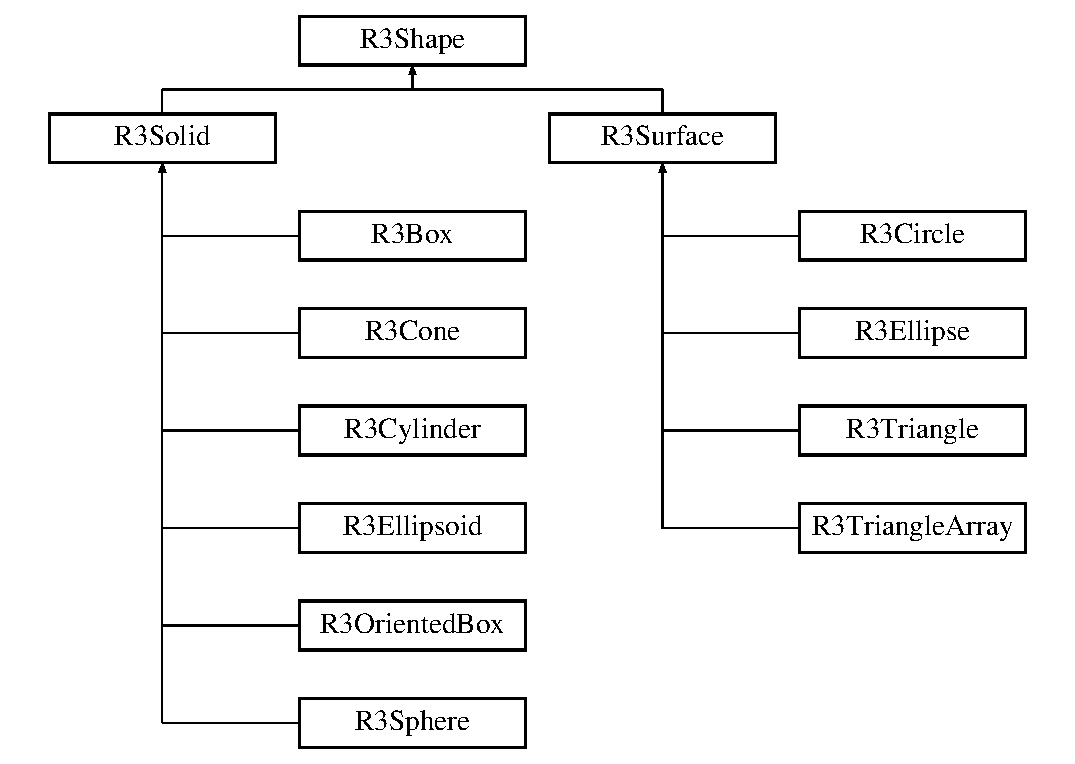
\includegraphics[height=8.000000cm]{class_r3_shape}
\end{center}
\end{figure}
\subsection*{Public Member Functions}
\begin{DoxyCompactItemize}
\item 
virtual const R\+N\+Boolean {\bfseries Is\+Point} (void) const \hypertarget{class_r3_shape_a65ccc5bc0e4af13ee97b79fe7cbdf0b6}{}\label{class_r3_shape_a65ccc5bc0e4af13ee97b79fe7cbdf0b6}

\item 
virtual const R\+N\+Boolean {\bfseries Is\+Curve} (void) const \hypertarget{class_r3_shape_a374534441c55187f1a6c169bf20a2a75}{}\label{class_r3_shape_a374534441c55187f1a6c169bf20a2a75}

\item 
virtual const R\+N\+Boolean {\bfseries Is\+Linear} (void) const \hypertarget{class_r3_shape_aee3efef05105e16493a81533c4550d52}{}\label{class_r3_shape_aee3efef05105e16493a81533c4550d52}

\item 
virtual const R\+N\+Boolean {\bfseries Is\+Surface} (void) const \hypertarget{class_r3_shape_a73708acac3b0a003b7db9fb0f2ef8f0f}{}\label{class_r3_shape_a73708acac3b0a003b7db9fb0f2ef8f0f}

\item 
virtual const R\+N\+Boolean {\bfseries Is\+Planar} (void) const \hypertarget{class_r3_shape_a8e57e4cb98dec5ee5ec00925b62209bb}{}\label{class_r3_shape_a8e57e4cb98dec5ee5ec00925b62209bb}

\item 
virtual const R\+N\+Boolean {\bfseries Is\+Solid} (void) const \hypertarget{class_r3_shape_addb240a469ab66276d9d854230eac6ea}{}\label{class_r3_shape_addb240a469ab66276d9d854230eac6ea}

\item 
virtual const R\+N\+Boolean {\bfseries Is\+Convex} (void) const \hypertarget{class_r3_shape_a939f0c9ebd6141d7f86c97bb7a36371b}{}\label{class_r3_shape_a939f0c9ebd6141d7f86c97bb7a36371b}

\item 
virtual const \hyperlink{class_r_n_interval}{R\+N\+Interval} {\bfseries N\+Facets} (void) const \hypertarget{class_r3_shape_a7074ed9033c6c86667ba97c63f9c387a}{}\label{class_r3_shape_a7074ed9033c6c86667ba97c63f9c387a}

\item 
virtual const R\+N\+Length {\bfseries Length} (void) const \hypertarget{class_r3_shape_aa5baaded6d628ee2ff091b05111446ec}{}\label{class_r3_shape_aa5baaded6d628ee2ff091b05111446ec}

\item 
virtual const R\+N\+Area {\bfseries Area} (void) const \hypertarget{class_r3_shape_adcd2aaa1a693e19bfca921fcc6d7a0b3}{}\label{class_r3_shape_adcd2aaa1a693e19bfca921fcc6d7a0b3}

\item 
virtual const R\+N\+Volume {\bfseries Volume} (void) const \hypertarget{class_r3_shape_a5a37c10a86d7a9820b3b5196d6a10462}{}\label{class_r3_shape_a5a37c10a86d7a9820b3b5196d6a10462}

\item 
virtual const \hyperlink{class_r3_point}{R3\+Point} {\bfseries Centroid} (void) const \hypertarget{class_r3_shape_a4c6ade5aa398118b7466f4d84e6826da}{}\label{class_r3_shape_a4c6ade5aa398118b7466f4d84e6826da}

\item 
virtual const \hyperlink{class_r3_point}{R3\+Point} {\bfseries Closest\+Point} (const \hyperlink{class_r3_point}{R3\+Point} \&point) const \hypertarget{class_r3_shape_a3f05de0550568443376095d7c837bf3b}{}\label{class_r3_shape_a3f05de0550568443376095d7c837bf3b}

\item 
virtual const \hyperlink{class_r3_point}{R3\+Point} {\bfseries Furthest\+Point} (const \hyperlink{class_r3_point}{R3\+Point} \&point) const \hypertarget{class_r3_shape_a41794b2d44a1c56c5cf73be83cb4165e}{}\label{class_r3_shape_a41794b2d44a1c56c5cf73be83cb4165e}

\item 
virtual const \hyperlink{class_r3_shape}{R3\+Shape} \& {\bfseries B\+Shape} (void) const \hypertarget{class_r3_shape_a0435c98d5c9fe998dcd58e49d75321b2}{}\label{class_r3_shape_a0435c98d5c9fe998dcd58e49d75321b2}

\item 
virtual const \hyperlink{class_r3_box}{R3\+Box} {\bfseries B\+Box} (void) const \hypertarget{class_r3_shape_a4b94120517811e7b20ffb636303c58b7}{}\label{class_r3_shape_a4b94120517811e7b20ffb636303c58b7}

\item 
virtual const \hyperlink{class_r3_sphere}{R3\+Sphere} {\bfseries B\+Sphere} (void) const \hypertarget{class_r3_shape_afb605cbb61b4920d6b243542f73bbc4c}{}\label{class_r3_shape_afb605cbb61b4920d6b243542f73bbc4c}

\item 
virtual void {\bfseries Transform} (const \hyperlink{class_r3_transformation}{R3\+Transformation} \&transformation)\hypertarget{class_r3_shape_a805967275158cebf6ba63469dfeacf6b}{}\label{class_r3_shape_a805967275158cebf6ba63469dfeacf6b}

\item 
virtual void {\bfseries Draw} (const \hyperlink{class_r_n_flags}{R3\+Draw\+Flags} draw\+\_\+flags=R3\+\_\+\+D\+E\+F\+A\+U\+L\+T\+\_\+\+D\+R\+A\+W\+\_\+\+F\+L\+A\+GS) const \hypertarget{class_r3_shape_a03ceca3e76e0eddfc2e23cef6b3facb3}{}\label{class_r3_shape_a03ceca3e76e0eddfc2e23cef6b3facb3}

\item 
virtual void {\bfseries Outline} (const \hyperlink{class_r_n_flags}{R3\+Draw\+Flags} draw\+\_\+flags=R3\+\_\+\+E\+D\+G\+E\+S\+\_\+\+D\+R\+A\+W\+\_\+\+F\+L\+AG) const \hypertarget{class_r3_shape_a46a22d218a4b5d18a8b66ed99696a556}{}\label{class_r3_shape_a46a22d218a4b5d18a8b66ed99696a556}

\item 
{\bfseries R\+N\+\_\+\+C\+L\+A\+S\+S\+\_\+\+T\+Y\+P\+E\+\_\+\+D\+E\+C\+L\+A\+R\+A\+T\+I\+O\+NS} (\hyperlink{class_r3_shape}{R3\+Shape})\hypertarget{class_r3_shape_a9b42dc3ad6ff8453eb728e8b16d68000}{}\label{class_r3_shape_a9b42dc3ad6ff8453eb728e8b16d68000}

\item 
{\bfseries R3\+\_\+\+S\+H\+A\+P\+E\+\_\+\+R\+E\+L\+A\+T\+I\+O\+N\+S\+H\+I\+P\+\_\+\+D\+E\+C\+L\+A\+R\+A\+T\+I\+O\+NS} (\hyperlink{class_r3_shape}{R3\+Shape})\hypertarget{class_r3_shape_a5ea506a416bbb72dcae64f36431cef95}{}\label{class_r3_shape_a5ea506a416bbb72dcae64f36431cef95}

\end{DoxyCompactItemize}


The documentation for this class was generated from the following files\+:\begin{DoxyCompactItemize}
\item 
R3\+Shapes/R3\+Shape.\+h\item 
R3\+Shapes/R3\+Shape.\+cpp\end{DoxyCompactItemize}

\hypertarget{class_r3_solid}{}\section{R3\+Solid Class Reference}
\label{class_r3_solid}\index{R3\+Solid@{R3\+Solid}}
Inheritance diagram for R3\+Solid\+:\begin{figure}[H]
\begin{center}
\leavevmode
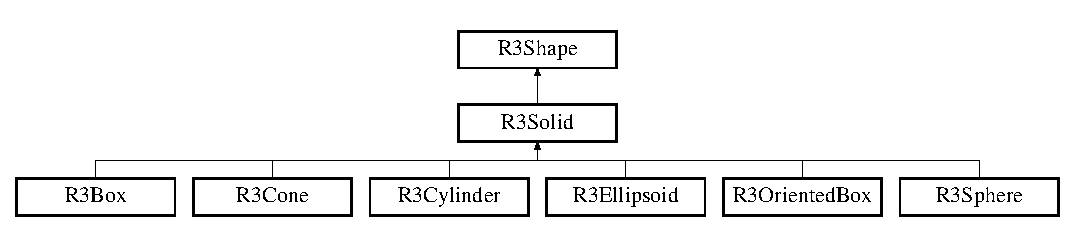
\includegraphics[height=2.666667cm]{class_r3_solid}
\end{center}
\end{figure}
\subsection*{Public Member Functions}
\begin{DoxyCompactItemize}
\item 
const R\+N\+Boolean {\bfseries Is\+Solid} (void) const \hypertarget{class_r3_solid_a19553484deb7afb7c4aed74cf933676d}{}\label{class_r3_solid_a19553484deb7afb7c4aed74cf933676d}

\end{DoxyCompactItemize}


The documentation for this class was generated from the following files\+:\begin{DoxyCompactItemize}
\item 
R3\+Shapes/R3\+Solid.\+h\item 
R3\+Shapes/R3\+Solid.\+cpp\end{DoxyCompactItemize}

\hypertarget{class_r3_span}{}\section{R3\+Span Class Reference}
\label{class_r3_span}\index{R3\+Span@{R3\+Span}}
\subsection*{Public Member Functions}
\begin{DoxyCompactItemize}
\item 
{\bfseries R3\+Span} (const \hyperlink{class_r3_span}{R3\+Span} \&span)\hypertarget{class_r3_span_af6722e4e0ca2b88613df50c0dccf495b}{}\label{class_r3_span_af6722e4e0ca2b88613df50c0dccf495b}

\item 
{\bfseries R3\+Span} (const \hyperlink{class_r3_point}{R3\+Point} \&point, const \hyperlink{class_r3_vector}{R3\+Vector} \&vector)\hypertarget{class_r3_span_a397f095aab62259ea85b4edb1a093806}{}\label{class_r3_span_a397f095aab62259ea85b4edb1a093806}

\item 
{\bfseries R3\+Span} (const \hyperlink{class_r3_point}{R3\+Point} \&point1, const \hyperlink{class_r3_point}{R3\+Point} \&point2)\hypertarget{class_r3_span_a31c0a79aefec3f5d1519fa4bec2422ce}{}\label{class_r3_span_a31c0a79aefec3f5d1519fa4bec2422ce}

\item 
{\bfseries R3\+Span} (R\+N\+Coord x1, R\+N\+Coord y1, R\+N\+Coord z1, R\+N\+Coord x2, R\+N\+Coord y2, R\+N\+Coord z2)\hypertarget{class_r3_span_a345ce02263964218a7e1d647ab521321}{}\label{class_r3_span_a345ce02263964218a7e1d647ab521321}

\item 
const \hyperlink{class_r3_point}{R3\+Point} \& {\bfseries Start} (void) const \hypertarget{class_r3_span_ac1f284804b7664f76c5b6f3d7b485551}{}\label{class_r3_span_ac1f284804b7664f76c5b6f3d7b485551}

\item 
const \hyperlink{class_r3_point}{R3\+Point} \& {\bfseries End} (void) const \hypertarget{class_r3_span_a7f2199b61961212eb950c9f28abe28bf}{}\label{class_r3_span_a7f2199b61961212eb950c9f28abe28bf}

\item 
const \hyperlink{class_r3_vector}{R3\+Vector} \& {\bfseries Vector} (void) const \hypertarget{class_r3_span_a5bfd6969ef381b3809a01ef7f055ad29}{}\label{class_r3_span_a5bfd6969ef381b3809a01ef7f055ad29}

\item 
const \hyperlink{class_r3_point}{R3\+Point} {\bfseries Point} (int k) const \hypertarget{class_r3_span_a7a9c37460b7051b17245f002eda33fb8}{}\label{class_r3_span_a7a9c37460b7051b17245f002eda33fb8}

\item 
const \hyperlink{class_r3_point}{R3\+Point} {\bfseries Point} (R\+N\+Scalar t) const \hypertarget{class_r3_span_a1f454d654bca6a900175c56ac48a78be}{}\label{class_r3_span_a1f454d654bca6a900175c56ac48a78be}

\item 
const \hyperlink{class_r3_point}{R3\+Point} \& {\bfseries operator\mbox{[}$\,$\mbox{]}} (int k) const \hypertarget{class_r3_span_aaddc31057dbe1861de7d03bbe06500dc}{}\label{class_r3_span_aaddc31057dbe1861de7d03bbe06500dc}

\item 
const \hyperlink{class_r3_ray}{R3\+Ray} \& {\bfseries Ray} (void) const \hypertarget{class_r3_span_a28005592e8c96a770470456bde4df119}{}\label{class_r3_span_a28005592e8c96a770470456bde4df119}

\item 
const \hyperlink{class_r3_line}{R3\+Line} \& {\bfseries Line} (void) const \hypertarget{class_r3_span_a099fd94d2323b9e89ef3adaef2b691a1}{}\label{class_r3_span_a099fd94d2323b9e89ef3adaef2b691a1}

\item 
const \hyperlink{class_r3_point}{R3\+Point} {\bfseries Midpoint} (void) const \hypertarget{class_r3_span_a6b083615a26cd4faf0bffdfd32eb644c}{}\label{class_r3_span_a6b083615a26cd4faf0bffdfd32eb644c}

\item 
const \hyperlink{class_r3_point}{R3\+Point} {\bfseries Centroid} (void) const \hypertarget{class_r3_span_a8f2eb5facc2b59b7992044278d13b483}{}\label{class_r3_span_a8f2eb5facc2b59b7992044278d13b483}

\item 
const \hyperlink{class_r3_box}{R3\+Box} {\bfseries B\+Box} (void) const \hypertarget{class_r3_span_ad92f003fe1bb1d27ba925b6163f1b24c}{}\label{class_r3_span_ad92f003fe1bb1d27ba925b6163f1b24c}

\item 
const \hyperlink{class_r3_sphere}{R3\+Sphere} {\bfseries B\+Sphere} (void) const \hypertarget{class_r3_span_a7732e1c626907763693a432d3bc7984f}{}\label{class_r3_span_a7732e1c626907763693a432d3bc7984f}

\item 
const R\+N\+Length {\bfseries Length} (void) const \hypertarget{class_r3_span_a1bf2fdf2921692dfd478c1f3e9a7fb4b}{}\label{class_r3_span_a1bf2fdf2921692dfd478c1f3e9a7fb4b}

\item 
const R\+N\+Scalar {\bfseries T} (const \hyperlink{class_r3_point}{R3\+Point} \&point) const \hypertarget{class_r3_span_ae5cd9ffa29772cf28e12183a544851b4}{}\label{class_r3_span_ae5cd9ffa29772cf28e12183a544851b4}

\item 
const R\+N\+Boolean {\bfseries Is\+Point} (void) const \hypertarget{class_r3_span_af83fa881cbe0eefc4f424e6e50c64e20}{}\label{class_r3_span_af83fa881cbe0eefc4f424e6e50c64e20}

\item 
const R\+N\+Boolean {\bfseries operator==} (const \hyperlink{class_r3_span}{R3\+Span} \&span) const \hypertarget{class_r3_span_a07595b5315b11a7a808d68d30c23f9a1}{}\label{class_r3_span_a07595b5315b11a7a808d68d30c23f9a1}

\item 
const R\+N\+Boolean {\bfseries operator!=} (const \hyperlink{class_r3_span}{R3\+Span} \&span) const \hypertarget{class_r3_span_a48293f15ba254f957b114233847727f3}{}\label{class_r3_span_a48293f15ba254f957b114233847727f3}

\item 
void {\bfseries Flip} (void)\hypertarget{class_r3_span_a84d35cbbbff9a38cee9f6f4d272fca68}{}\label{class_r3_span_a84d35cbbbff9a38cee9f6f4d272fca68}

\item 
void {\bfseries Mirror} (const \hyperlink{class_r3_plane}{R3\+Plane} \&plane)\hypertarget{class_r3_span_a9d54987bc3760e31fd0103cf6947f84d}{}\label{class_r3_span_a9d54987bc3760e31fd0103cf6947f84d}

\item 
void {\bfseries Translate} (const \hyperlink{class_r3_vector}{R3\+Vector} \&vector)\hypertarget{class_r3_span_a60ba97b071b5fb4518f1624d4b2c7f5f}{}\label{class_r3_span_a60ba97b071b5fb4518f1624d4b2c7f5f}

\item 
void {\bfseries Reposition} (int k, const \hyperlink{class_r3_point}{R3\+Point} \&point)\hypertarget{class_r3_span_a62b4fbe8c1e5120dbce8c9d4cc9a0a15}{}\label{class_r3_span_a62b4fbe8c1e5120dbce8c9d4cc9a0a15}

\item 
void {\bfseries Align} (const \hyperlink{class_r3_vector}{R3\+Vector} \&vector)\hypertarget{class_r3_span_a3daf9e992ab12d9d424cdd3b4e9821ca}{}\label{class_r3_span_a3daf9e992ab12d9d424cdd3b4e9821ca}

\item 
void {\bfseries Transform} (const \hyperlink{class_r3_transformation}{R3\+Transformation} \&transformation)\hypertarget{class_r3_span_ab0e85677f78f12fbd1a1c3c0a17f066e}{}\label{class_r3_span_ab0e85677f78f12fbd1a1c3c0a17f066e}

\item 
void {\bfseries Inverse\+Transform} (const \hyperlink{class_r3_transformation}{R3\+Transformation} \&transformation)\hypertarget{class_r3_span_add3ed3a5f7458b7328634b7929f82dca}{}\label{class_r3_span_add3ed3a5f7458b7328634b7929f82dca}

\item 
void {\bfseries Reset} (const \hyperlink{class_r3_point}{R3\+Point} \&point1, const \hyperlink{class_r3_point}{R3\+Point} \&point2)\hypertarget{class_r3_span_a64b035877a24244951eb700f1e55c022}{}\label{class_r3_span_a64b035877a24244951eb700f1e55c022}

\item 
R\+N\+Class\+ID {\bfseries Clip} (const \hyperlink{class_r3_plane}{R3\+Plane} \&plane)\hypertarget{class_r3_span_a90c362a1cfea5b2053cdb0cf3c624216}{}\label{class_r3_span_a90c362a1cfea5b2053cdb0cf3c624216}

\item 
void {\bfseries Draw} (void) const \hypertarget{class_r3_span_ab72e55af15ad8a4c5f17d9e9b3a4b06e}{}\label{class_r3_span_ab72e55af15ad8a4c5f17d9e9b3a4b06e}

\item 
\hyperlink{class_r3_span}{R3\+Span} {\bfseries operator-\/} (void) const \hypertarget{class_r3_span_a193206788b9e14243c72f71ffff95b4a}{}\label{class_r3_span_a193206788b9e14243c72f71ffff95b4a}

\end{DoxyCompactItemize}


The documentation for this class was generated from the following files\+:\begin{DoxyCompactItemize}
\item 
R3\+Shapes/R3\+Span.\+h\item 
R3\+Shapes/R3\+Draw.\+cpp\item 
R3\+Shapes/R3\+Span.\+cpp\end{DoxyCompactItemize}

\hypertarget{class_r3_sphere}{}\section{R3\+Sphere Class Reference}
\label{class_r3_sphere}\index{R3\+Sphere@{R3\+Sphere}}
Inheritance diagram for R3\+Sphere\+:\begin{figure}[H]
\begin{center}
\leavevmode
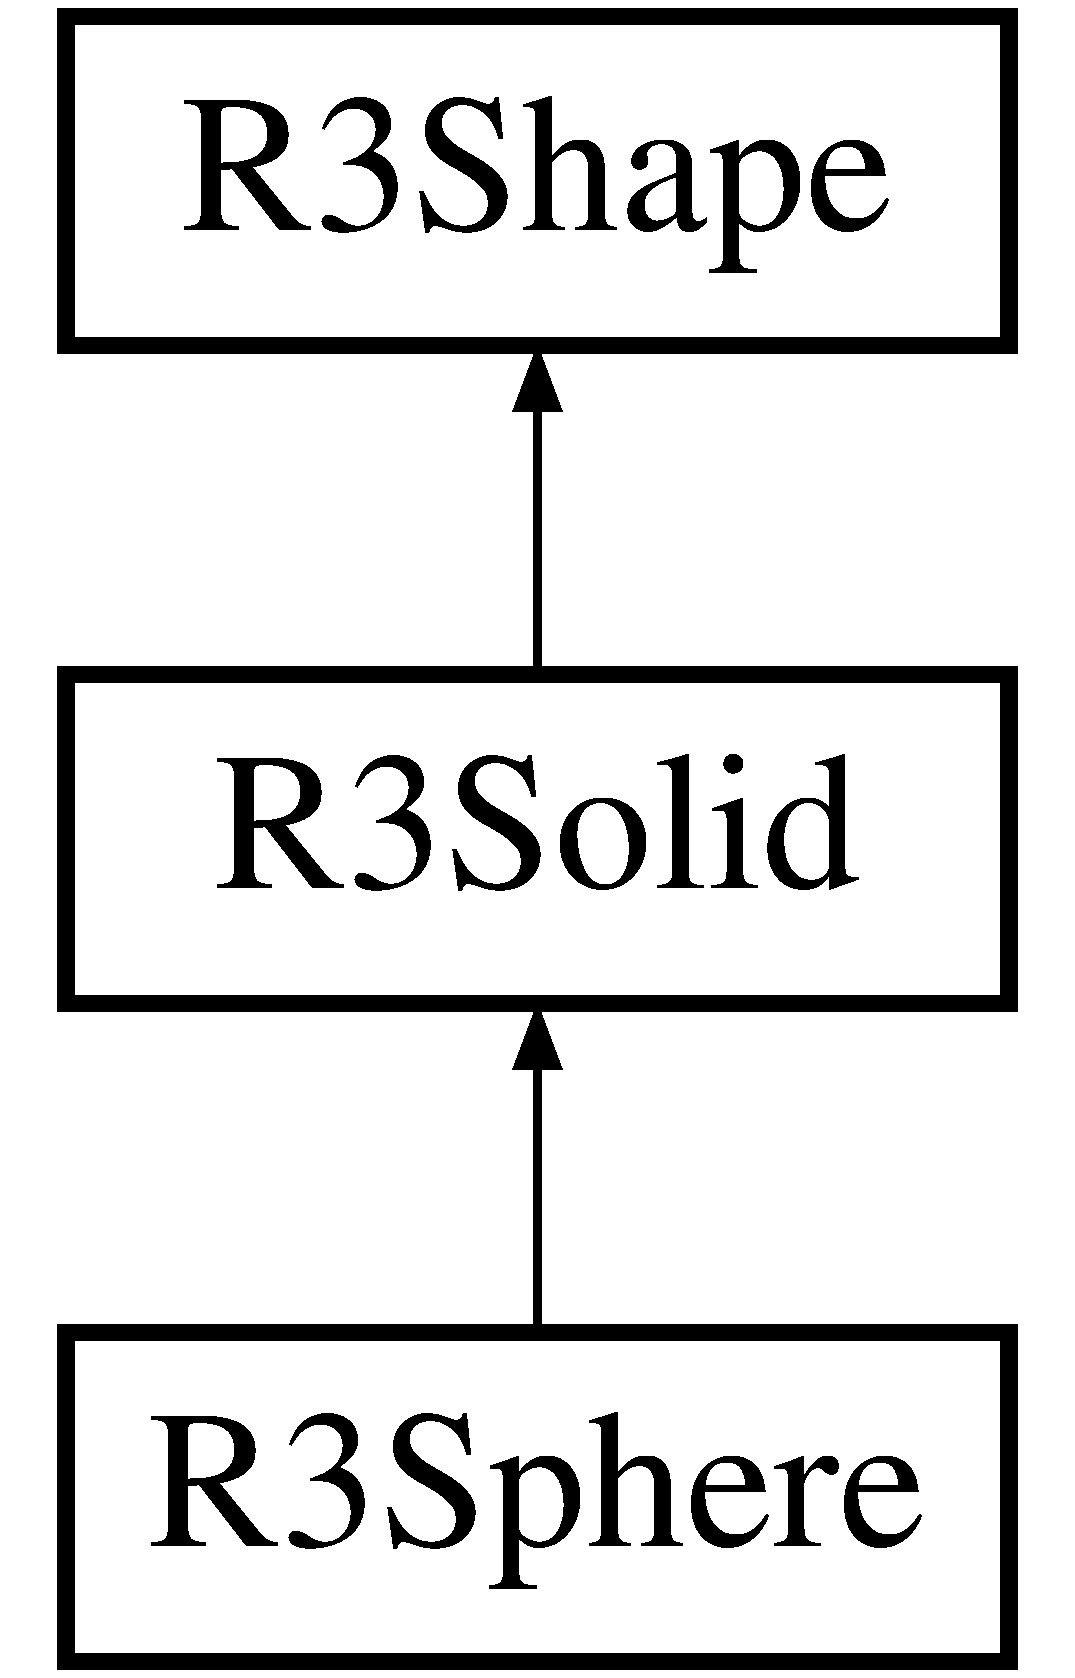
\includegraphics[height=3.000000cm]{class_r3_sphere}
\end{center}
\end{figure}
\subsection*{Public Member Functions}
\begin{DoxyCompactItemize}
\item 
{\bfseries R3\+Sphere} (const \hyperlink{class_r3_sphere}{R3\+Sphere} \&sphere)\hypertarget{class_r3_sphere_a74f08d961e787c07c576b7a64e6137bf}{}\label{class_r3_sphere_a74f08d961e787c07c576b7a64e6137bf}

\item 
{\bfseries R3\+Sphere} (const \hyperlink{class_r3_point}{R3\+Point} \&center, R\+N\+Length radius)\hypertarget{class_r3_sphere_afe12687419c6e731367b34dbe39137eb}{}\label{class_r3_sphere_afe12687419c6e731367b34dbe39137eb}

\item 
const \hyperlink{class_r3_point}{R3\+Point} \& {\bfseries Center} (void) const \hypertarget{class_r3_sphere_ad2b58bb0c58a81f1ca9e8e0d39287f3d}{}\label{class_r3_sphere_ad2b58bb0c58a81f1ca9e8e0d39287f3d}

\item 
const R\+N\+Length {\bfseries Radius} (void) const \hypertarget{class_r3_sphere_a704678a914c0c1762908d7d639ee973c}{}\label{class_r3_sphere_a704678a914c0c1762908d7d639ee973c}

\item 
const R\+N\+Boolean {\bfseries Is\+Empty} (void) const \hypertarget{class_r3_sphere_a4b7b1d16a1d689bd3fc4d52d98a9cbc6}{}\label{class_r3_sphere_a4b7b1d16a1d689bd3fc4d52d98a9cbc6}

\item 
const R\+N\+Boolean {\bfseries Is\+Finite} (void) const \hypertarget{class_r3_sphere_a30b6e2ce321b378257d5fe195025a6aa}{}\label{class_r3_sphere_a30b6e2ce321b378257d5fe195025a6aa}

\item 
virtual const R\+N\+Boolean {\bfseries Is\+Point} (void) const \hypertarget{class_r3_sphere_a45d13b09b5180360ac09ee96bd5d4de7}{}\label{class_r3_sphere_a45d13b09b5180360ac09ee96bd5d4de7}

\item 
virtual const R\+N\+Boolean {\bfseries Is\+Linear} (void) const \hypertarget{class_r3_sphere_af0ae99556f80eb91aaf72593f430e709}{}\label{class_r3_sphere_af0ae99556f80eb91aaf72593f430e709}

\item 
virtual const R\+N\+Boolean {\bfseries Is\+Planar} (void) const \hypertarget{class_r3_sphere_a91bae65fd321234e491ff75dae2969cb}{}\label{class_r3_sphere_a91bae65fd321234e491ff75dae2969cb}

\item 
virtual const R\+N\+Boolean {\bfseries Is\+Convex} (void) const \hypertarget{class_r3_sphere_a9facb28d0c47ef3b822371c27511eb78}{}\label{class_r3_sphere_a9facb28d0c47ef3b822371c27511eb78}

\item 
virtual const \hyperlink{class_r_n_interval}{R\+N\+Interval} {\bfseries N\+Facets} (void) const \hypertarget{class_r3_sphere_a48201ee9b34adb2e9338162eec55d61e}{}\label{class_r3_sphere_a48201ee9b34adb2e9338162eec55d61e}

\item 
virtual const R\+N\+Area {\bfseries Area} (void) const \hypertarget{class_r3_sphere_a00fea0038d75f61da89f6d4c2c61468d}{}\label{class_r3_sphere_a00fea0038d75f61da89f6d4c2c61468d}

\item 
virtual const R\+N\+Volume {\bfseries Volume} (void) const \hypertarget{class_r3_sphere_a1e5f94290ff0c0cffb50a2e4a480df14}{}\label{class_r3_sphere_a1e5f94290ff0c0cffb50a2e4a480df14}

\item 
virtual const \hyperlink{class_r3_point}{R3\+Point} {\bfseries Centroid} (void) const \hypertarget{class_r3_sphere_a3ea4f238c55334f8d05d08db6fc6c7ec}{}\label{class_r3_sphere_a3ea4f238c55334f8d05d08db6fc6c7ec}

\item 
virtual const \hyperlink{class_r3_point}{R3\+Point} {\bfseries Closest\+Point} (const \hyperlink{class_r3_point}{R3\+Point} \&point) const \hypertarget{class_r3_sphere_ae76c7d580e8cc17dadee06753adf37ff}{}\label{class_r3_sphere_ae76c7d580e8cc17dadee06753adf37ff}

\item 
virtual const \hyperlink{class_r3_point}{R3\+Point} {\bfseries Furthest\+Point} (const \hyperlink{class_r3_point}{R3\+Point} \&point) const \hypertarget{class_r3_sphere_a801de3885443b757fda2af2d1c83e7d5}{}\label{class_r3_sphere_a801de3885443b757fda2af2d1c83e7d5}

\item 
virtual const \hyperlink{class_r3_shape}{R3\+Shape} \& {\bfseries B\+Shape} (void) const \hypertarget{class_r3_sphere_a2fc29cd666cd8ad6d3ea8453f7fe20eb}{}\label{class_r3_sphere_a2fc29cd666cd8ad6d3ea8453f7fe20eb}

\item 
virtual const \hyperlink{class_r3_box}{R3\+Box} {\bfseries B\+Box} (void) const \hypertarget{class_r3_sphere_a880d6ddda6599979cfdace0793c5adee}{}\label{class_r3_sphere_a880d6ddda6599979cfdace0793c5adee}

\item 
virtual const \hyperlink{class_r3_sphere}{R3\+Sphere} {\bfseries B\+Sphere} (void) const \hypertarget{class_r3_sphere_a97a92f1b36e6e0f9addca653d298c17f}{}\label{class_r3_sphere_a97a92f1b36e6e0f9addca653d298c17f}

\item 
virtual void {\bfseries Empty} (void)\hypertarget{class_r3_sphere_a55d84ffe26354fb412267d5290056b74}{}\label{class_r3_sphere_a55d84ffe26354fb412267d5290056b74}

\item 
virtual void {\bfseries Translate} (const \hyperlink{class_r3_vector}{R3\+Vector} \&vector)\hypertarget{class_r3_sphere_adb3e1980a65678bf9a1ea38452e56996}{}\label{class_r3_sphere_adb3e1980a65678bf9a1ea38452e56996}

\item 
virtual void {\bfseries Reposition} (const \hyperlink{class_r3_point}{R3\+Point} \&center)\hypertarget{class_r3_sphere_acdf84916c39e97cc88f3f29f3dc52c82}{}\label{class_r3_sphere_acdf84916c39e97cc88f3f29f3dc52c82}

\item 
virtual void {\bfseries Resize} (R\+N\+Length radius)\hypertarget{class_r3_sphere_a71402fa79698dce9b752bbbd69c8a2f6}{}\label{class_r3_sphere_a71402fa79698dce9b752bbbd69c8a2f6}

\item 
virtual void {\bfseries Transform} (const \hyperlink{class_r3_transformation}{R3\+Transformation} \&transformation)\hypertarget{class_r3_sphere_ae02687a899eb193db0b5248d0685fbf0}{}\label{class_r3_sphere_ae02687a899eb193db0b5248d0685fbf0}

\item 
virtual void {\bfseries Draw} (const \hyperlink{class_r_n_flags}{R3\+Draw\+Flags} draw\+\_\+flags=R3\+\_\+\+D\+E\+F\+A\+U\+L\+T\+\_\+\+D\+R\+A\+W\+\_\+\+F\+L\+A\+GS) const \hypertarget{class_r3_sphere_a5248547a73378021e3c8e6c1b28f9220}{}\label{class_r3_sphere_a5248547a73378021e3c8e6c1b28f9220}

\item 
{\bfseries R\+N\+\_\+\+C\+L\+A\+S\+S\+\_\+\+T\+Y\+P\+E\+\_\+\+D\+E\+C\+L\+A\+R\+A\+T\+I\+O\+NS} (\hyperlink{class_r3_sphere}{R3\+Sphere})\hypertarget{class_r3_sphere_af14b91c5a902f15ac9a352ac5367b7a1}{}\label{class_r3_sphere_af14b91c5a902f15ac9a352ac5367b7a1}

\item 
{\bfseries R3\+\_\+\+S\+H\+A\+P\+E\+\_\+\+R\+E\+L\+A\+T\+I\+O\+N\+S\+H\+I\+P\+\_\+\+D\+E\+C\+L\+A\+R\+A\+T\+I\+O\+NS} (\hyperlink{class_r3_sphere}{R3\+Sphere})\hypertarget{class_r3_sphere_a14cadaaebbe4fb28a83b9a958cbf94e3}{}\label{class_r3_sphere_a14cadaaebbe4fb28a83b9a958cbf94e3}

\end{DoxyCompactItemize}


The documentation for this class was generated from the following files\+:\begin{DoxyCompactItemize}
\item 
R3\+Shapes/R3\+Sphere.\+h\item 
R3\+Shapes/R3\+Draw.\+cpp\item 
R3\+Shapes/R3\+Sphere.\+cpp\end{DoxyCompactItemize}

\hypertarget{class_r3_spot_light}{}\section{R3\+Spot\+Light Class Reference}
\label{class_r3_spot_light}\index{R3\+Spot\+Light@{R3\+Spot\+Light}}
Inheritance diagram for R3\+Spot\+Light\+:\begin{figure}[H]
\begin{center}
\leavevmode
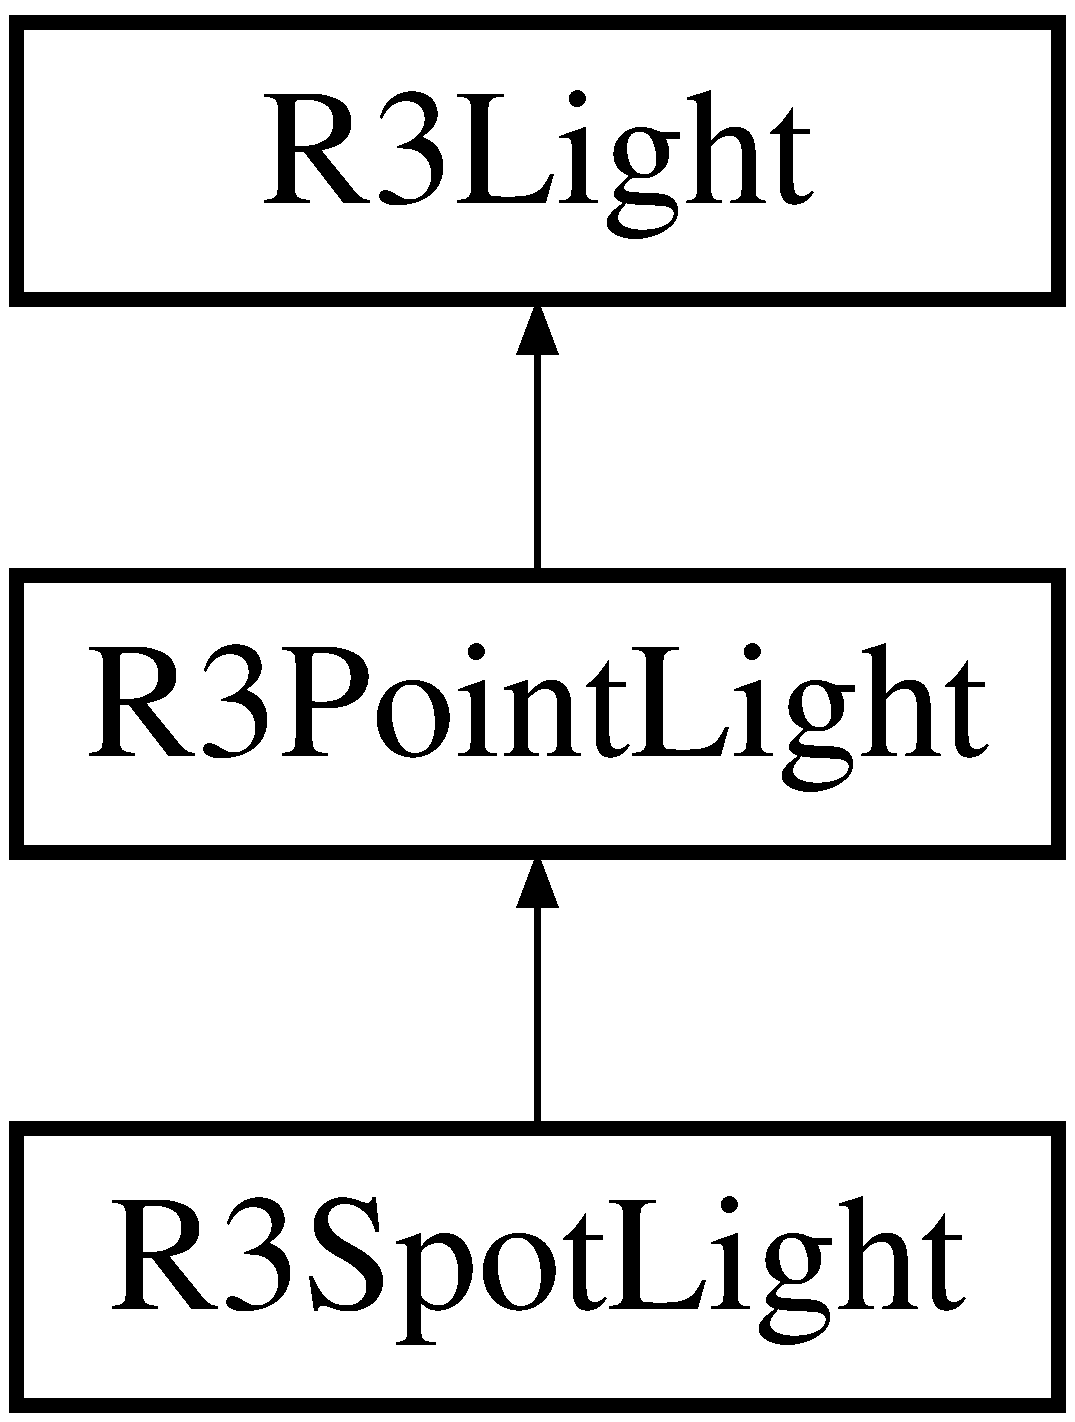
\includegraphics[height=3.000000cm]{class_r3_spot_light}
\end{center}
\end{figure}
\subsection*{Public Member Functions}
\begin{DoxyCompactItemize}
\item 
{\bfseries R3\+Spot\+Light} (const \hyperlink{class_r3_spot_light}{R3\+Spot\+Light} \&light)\hypertarget{class_r3_spot_light_a7f96a12fa6966f9ff80f364623739b77}{}\label{class_r3_spot_light_a7f96a12fa6966f9ff80f364623739b77}

\item 
{\bfseries R3\+Spot\+Light} (const \hyperlink{class_r3_point}{R3\+Point} \&position, const \hyperlink{class_r3_vector}{R3\+Vector} \&direction, const \hyperlink{class_r_n_rgb}{R\+N\+Rgb} \&color, R\+N\+Scalar dropoffrate=0.\+0, R\+N\+Angle cutoffangle=0.\+785398, R\+N\+Scalar intensity=1.\+0, R\+N\+Boolean active=T\+R\+UE, R\+N\+Scalar ca=0, R\+N\+Scalar la=0, R\+N\+Scalar qa=1)\hypertarget{class_r3_spot_light_a14ff94d1396aa573bf9fd8d71cf18262}{}\label{class_r3_spot_light_a14ff94d1396aa573bf9fd8d71cf18262}

\item 
const \hyperlink{class_r3_vector}{R3\+Vector} \& {\bfseries Direction} (void) const \hypertarget{class_r3_spot_light_a6b0c49b8b45f3ff0b8e0fde98dddd713}{}\label{class_r3_spot_light_a6b0c49b8b45f3ff0b8e0fde98dddd713}

\item 
const R\+N\+Scalar {\bfseries Drop\+Off\+Rate} (void) const \hypertarget{class_r3_spot_light_a248da1cf73c4718eadf1f31fc19698e4}{}\label{class_r3_spot_light_a248da1cf73c4718eadf1f31fc19698e4}

\item 
const R\+N\+Angle {\bfseries Cut\+Off\+Angle} (void) const \hypertarget{class_r3_spot_light_ab95d89e720b6679a2b5b3ee8bcd01341}{}\label{class_r3_spot_light_ab95d89e720b6679a2b5b3ee8bcd01341}

\item 
virtual void {\bfseries Set\+Direction} (const \hyperlink{class_r3_vector}{R3\+Vector} \&direction)\hypertarget{class_r3_spot_light_ae88c52971d49a195f7b4122ff7ec4ef9}{}\label{class_r3_spot_light_ae88c52971d49a195f7b4122ff7ec4ef9}

\item 
virtual void {\bfseries Set\+Drop\+Off\+Rate} (R\+N\+Scalar dropoffrate)\hypertarget{class_r3_spot_light_a2280ba3a723e9994b2d43c704f2ab553}{}\label{class_r3_spot_light_a2280ba3a723e9994b2d43c704f2ab553}

\item 
virtual void {\bfseries Set\+Cut\+Off\+Angle} (R\+N\+Angle cutoffangle)\hypertarget{class_r3_spot_light_a7db2a49de305167b9132ec745967ccb8}{}\label{class_r3_spot_light_a7db2a49de305167b9132ec745967ccb8}

\item 
virtual R\+N\+Scalar {\bfseries Intensity\+At\+Point} (const \hyperlink{class_r3_point}{R3\+Point} \&point) const \hypertarget{class_r3_spot_light_a22392975bee5fdeb193740651e4e3a9f}{}\label{class_r3_spot_light_a22392975bee5fdeb193740651e4e3a9f}

\item 
virtual void {\bfseries Draw} (int i) const \hypertarget{class_r3_spot_light_a32227f8c75c9eb1aacf3895ff230a5f1}{}\label{class_r3_spot_light_a32227f8c75c9eb1aacf3895ff230a5f1}

\item 
{\bfseries R\+N\+\_\+\+C\+L\+A\+S\+S\+\_\+\+T\+Y\+P\+E\+\_\+\+D\+E\+C\+L\+A\+R\+A\+T\+I\+O\+NS} (\hyperlink{class_r3_spot_light}{R3\+Spot\+Light})\hypertarget{class_r3_spot_light_accba49bf23c8839b97f413a21e04014f}{}\label{class_r3_spot_light_accba49bf23c8839b97f413a21e04014f}

\end{DoxyCompactItemize}


The documentation for this class was generated from the following files\+:\begin{DoxyCompactItemize}
\item 
R3\+Graphics/R3\+Spot\+Light.\+h\item 
R3\+Graphics/R3\+Spot\+Light.\+cpp\end{DoxyCompactItemize}

\hypertarget{class_r3_surface}{}\section{R3\+Surface Class Reference}
\label{class_r3_surface}\index{R3\+Surface@{R3\+Surface}}
Inheritance diagram for R3\+Surface\+:\begin{figure}[H]
\begin{center}
\leavevmode
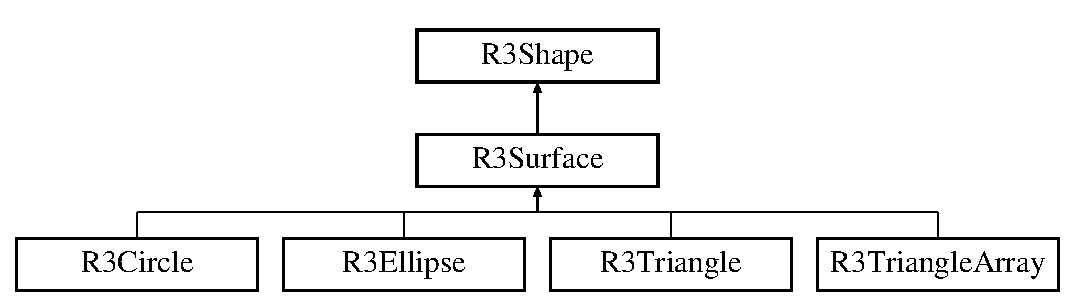
\includegraphics[height=3.000000cm]{class_r3_surface}
\end{center}
\end{figure}
\subsection*{Public Member Functions}
\begin{DoxyCompactItemize}
\item 
const R\+N\+Boolean {\bfseries Is\+Surface} (void) const \hypertarget{class_r3_surface_a3f1105fa345ce0e7f1a754b2d0be629c}{}\label{class_r3_surface_a3f1105fa345ce0e7f1a754b2d0be629c}

\end{DoxyCompactItemize}


The documentation for this class was generated from the following files\+:\begin{DoxyCompactItemize}
\item 
R3\+Shapes/R3\+Surface.\+h\item 
R3\+Shapes/R3\+Surface.\+cpp\end{DoxyCompactItemize}

\hypertarget{class_r3_surfel}{}\section{R3\+Surfel Class Reference}
\label{class_r3_surfel}\index{R3\+Surfel@{R3\+Surfel}}
\subsection*{Public Member Functions}
\begin{DoxyCompactItemize}
\item 
{\bfseries R3\+Surfel} (float px, float py, float pz, unsigned char r=0, unsigned char g=0, unsigned char b=0, R\+N\+Boolean aerial=F\+A\+L\+SE)\hypertarget{class_r3_surfel_a66b27b2fb91263248e57bd658349c4f0}{}\label{class_r3_surfel_a66b27b2fb91263248e57bd658349c4f0}

\item 
{\bfseries R3\+Surfel} (float px, float py, float pz, float nx, float ny, float nz, float radius=0, unsigned char r=0, unsigned char g=0, unsigned char b=0, unsigned char flags=0)\hypertarget{class_r3_surfel_aa71b74777feac648eb830182f55b834a}{}\label{class_r3_surfel_aa71b74777feac648eb830182f55b834a}

\item 
float {\bfseries X} (void) const \hypertarget{class_r3_surfel_ae812160059c24a38c646ddff8f3aafce}{}\label{class_r3_surfel_ae812160059c24a38c646ddff8f3aafce}

\item 
float {\bfseries Y} (void) const \hypertarget{class_r3_surfel_ad2565bcc563ab663f4519a2026f39b80}{}\label{class_r3_surfel_ad2565bcc563ab663f4519a2026f39b80}

\item 
float {\bfseries Z} (void) const \hypertarget{class_r3_surfel_aa49f3595f5080b3bee482f9d6ed457b4}{}\label{class_r3_surfel_aa49f3595f5080b3bee482f9d6ed457b4}

\item 
float {\bfseries Coord} (int dimension) const \hypertarget{class_r3_surfel_a7e645564ba4d3794dc5cd32e2e692fc2}{}\label{class_r3_surfel_a7e645564ba4d3794dc5cd32e2e692fc2}

\item 
const float $\ast$ {\bfseries Coords} (void) const \hypertarget{class_r3_surfel_a1ae079d2dad433feff504adc601ada30}{}\label{class_r3_surfel_a1ae079d2dad433feff504adc601ada30}

\item 
float {\bfseries NX} (void) const \hypertarget{class_r3_surfel_a7e1e615670828c7b94f2c8c8fc837cb1}{}\label{class_r3_surfel_a7e1e615670828c7b94f2c8c8fc837cb1}

\item 
float {\bfseries NY} (void) const \hypertarget{class_r3_surfel_a7dc895b6d28d184518e1fe2b09cb6a69}{}\label{class_r3_surfel_a7dc895b6d28d184518e1fe2b09cb6a69}

\item 
float {\bfseries NZ} (void) const \hypertarget{class_r3_surfel_a445371a7e7baed5c2099473bf823613f}{}\label{class_r3_surfel_a445371a7e7baed5c2099473bf823613f}

\item 
float {\bfseries Normal\+Coord} (int dimension) const \hypertarget{class_r3_surfel_a5b3ce26ef86c85fa155f575b0c441739}{}\label{class_r3_surfel_a5b3ce26ef86c85fa155f575b0c441739}

\item 
const float $\ast$ {\bfseries Normal\+Coords} (void) const \hypertarget{class_r3_surfel_ace25c8449707b52079df59fe513e80d4}{}\label{class_r3_surfel_ace25c8449707b52079df59fe513e80d4}

\item 
unsigned char {\bfseries R} (void) const \hypertarget{class_r3_surfel_a85c54b86829073b779b54776df5e0826}{}\label{class_r3_surfel_a85c54b86829073b779b54776df5e0826}

\item 
unsigned char {\bfseries G} (void) const \hypertarget{class_r3_surfel_a25e44ca53d42c3de2d287217d3e81279}{}\label{class_r3_surfel_a25e44ca53d42c3de2d287217d3e81279}

\item 
unsigned char {\bfseries B} (void) const \hypertarget{class_r3_surfel_afe210241ea742850736aa8065ab9ea9d}{}\label{class_r3_surfel_afe210241ea742850736aa8065ab9ea9d}

\item 
const unsigned char $\ast$ {\bfseries Color} (void) const \hypertarget{class_r3_surfel_a2e2472fdb8846ebedcef8520400fd57a}{}\label{class_r3_surfel_a2e2472fdb8846ebedcef8520400fd57a}

\item 
\hyperlink{class_r_n_rgb}{R\+N\+Rgb} {\bfseries Rgb} (void) const \hypertarget{class_r3_surfel_ad32689888880a16d6134ab5a283632ee}{}\label{class_r3_surfel_ad32689888880a16d6134ab5a283632ee}

\item 
float {\bfseries Radius} (void) const \hypertarget{class_r3_surfel_a10be2b9bd6406edb815329c3e137112f}{}\label{class_r3_surfel_a10be2b9bd6406edb815329c3e137112f}

\item 
R\+N\+Boolean {\bfseries Is\+Active} (void) const \hypertarget{class_r3_surfel_af9583a53431a81e940db541a2c1b66a9}{}\label{class_r3_surfel_af9583a53431a81e940db541a2c1b66a9}

\item 
R\+N\+Boolean {\bfseries Is\+Marked} (void) const \hypertarget{class_r3_surfel_abf64bb4387d4ae280911846b56594c1f}{}\label{class_r3_surfel_abf64bb4387d4ae280911846b56594c1f}

\item 
R\+N\+Boolean {\bfseries Is\+Aerial} (void) const \hypertarget{class_r3_surfel_ab94fba832be43a24ec44624fb0c74c92}{}\label{class_r3_surfel_ab94fba832be43a24ec44624fb0c74c92}

\item 
R\+N\+Boolean {\bfseries Is\+Terrestrial} (void) const \hypertarget{class_r3_surfel_a97072c98883341a05036c32e38551055}{}\label{class_r3_surfel_a97072c98883341a05036c32e38551055}

\item 
R\+N\+Boolean {\bfseries Is\+On\+Silhouette\+Boundary} (void) const \hypertarget{class_r3_surfel_a1d7f24f5ed8130f0188689388bbd4eda}{}\label{class_r3_surfel_a1d7f24f5ed8130f0188689388bbd4eda}

\item 
R\+N\+Boolean {\bfseries Is\+On\+Shadow\+Boundary} (void) const \hypertarget{class_r3_surfel_ae3b3bd069c075607c24b48011acdcb1d}{}\label{class_r3_surfel_ae3b3bd069c075607c24b48011acdcb1d}

\item 
R\+N\+Boolean {\bfseries Is\+On\+Border\+Boundary} (void) const \hypertarget{class_r3_surfel_a778d1b901e038a733c07fc9d1cd02bae}{}\label{class_r3_surfel_a778d1b901e038a733c07fc9d1cd02bae}

\item 
R\+N\+Boolean {\bfseries Is\+On\+Boundary} (void) const \hypertarget{class_r3_surfel_add276e23464147a768f5929e7c974e5b}{}\label{class_r3_surfel_add276e23464147a768f5929e7c974e5b}

\item 
R\+N\+Boolean {\bfseries Has\+Normal} (void) const \hypertarget{class_r3_surfel_a682a13d2887e071f441309485acf7458}{}\label{class_r3_surfel_a682a13d2887e071f441309485acf7458}

\item 
unsigned char {\bfseries Flags} (void) const \hypertarget{class_r3_surfel_acbc8c1d315cfbad47950f439a7d5efd7}{}\label{class_r3_surfel_acbc8c1d315cfbad47950f439a7d5efd7}

\item 
void {\bfseries Set\+Coords} (float x, float y, float z)\hypertarget{class_r3_surfel_a955683caa3b8332f46c3fe4dae2f4a1a}{}\label{class_r3_surfel_a955683caa3b8332f46c3fe4dae2f4a1a}

\item 
void {\bfseries Set\+Coords} (const float $\ast$xyz)\hypertarget{class_r3_surfel_a95b10839c05fde3d1d23a80542450c8d}{}\label{class_r3_surfel_a95b10839c05fde3d1d23a80542450c8d}

\item 
void {\bfseries Set\+Normal} (float x, float y, float z)\hypertarget{class_r3_surfel_a3988e8403ed0db6cd635b7ce383971ac}{}\label{class_r3_surfel_a3988e8403ed0db6cd635b7ce383971ac}

\item 
void {\bfseries Set\+Normal} (const float $\ast$xyz)\hypertarget{class_r3_surfel_a03b8ee25d9827ef4ef54dc8fbd30b5a5}{}\label{class_r3_surfel_a03b8ee25d9827ef4ef54dc8fbd30b5a5}

\item 
void {\bfseries Set\+Radius} (float radius)\hypertarget{class_r3_surfel_a2372ea8b1f414fd2ba1ebcf15dae4f52}{}\label{class_r3_surfel_a2372ea8b1f414fd2ba1ebcf15dae4f52}

\item 
void {\bfseries Set\+Color} (unsigned char r, unsigned char g, unsigned char b)\hypertarget{class_r3_surfel_a810907ecb71272cca1a6b5475aab2c0f}{}\label{class_r3_surfel_a810907ecb71272cca1a6b5475aab2c0f}

\item 
void {\bfseries Set\+Color} (const unsigned char $\ast$rgb)\hypertarget{class_r3_surfel_aafe3d8b4430df0fe35f96475427774e9}{}\label{class_r3_surfel_aafe3d8b4430df0fe35f96475427774e9}

\item 
void {\bfseries Set\+Color} (const \hyperlink{class_r_n_rgb}{R\+N\+Rgb} \&rgb)\hypertarget{class_r3_surfel_abb7947e550b3c4f2b91e5bb658045e96}{}\label{class_r3_surfel_abb7947e550b3c4f2b91e5bb658045e96}

\item 
void {\bfseries Set\+Aerial} (R\+N\+Boolean aerial=T\+R\+UE)\hypertarget{class_r3_surfel_ad2433357c63f4f21248bc6c731118dc4}{}\label{class_r3_surfel_ad2433357c63f4f21248bc6c731118dc4}

\item 
void {\bfseries Set\+Silhouette\+Boundary} (R\+N\+Boolean boundary=T\+R\+UE)\hypertarget{class_r3_surfel_a7deef87c064105c700faf4959153d82a}{}\label{class_r3_surfel_a7deef87c064105c700faf4959153d82a}

\item 
void {\bfseries Set\+Shadow\+Boundary} (R\+N\+Boolean boundary=T\+R\+UE)\hypertarget{class_r3_surfel_a51157685daeba803b1cb272c3c2096df}{}\label{class_r3_surfel_a51157685daeba803b1cb272c3c2096df}

\item 
void {\bfseries Set\+Border\+Boundary} (R\+N\+Boolean boundary=T\+R\+UE)\hypertarget{class_r3_surfel_ab7e804a79d200977837bca67888ab65c}{}\label{class_r3_surfel_ab7e804a79d200977837bca67888ab65c}

\item 
void {\bfseries Set\+Mark} (R\+N\+Boolean mark=T\+R\+UE)\hypertarget{class_r3_surfel_aebef5adb1685c967b33a005a79f26411}{}\label{class_r3_surfel_aebef5adb1685c967b33a005a79f26411}

\item 
void {\bfseries Set\+Active} (R\+N\+Boolean active=T\+R\+UE)\hypertarget{class_r3_surfel_a27c7598605cbef7e978d15b2c8c59711}{}\label{class_r3_surfel_a27c7598605cbef7e978d15b2c8c59711}

\item 
void {\bfseries Set\+Flags} (unsigned char flags)\hypertarget{class_r3_surfel_a19bd398afff05e305c58a88b92b00266}{}\label{class_r3_surfel_a19bd398afff05e305c58a88b92b00266}

\item 
void {\bfseries Draw} (\hyperlink{class_r_n_flags}{R\+N\+Flags} flags=R3\+\_\+\+S\+U\+R\+F\+E\+L\+\_\+\+D\+E\+F\+A\+U\+L\+T\+\_\+\+D\+R\+A\+W\+\_\+\+F\+L\+A\+GS) const \hypertarget{class_r3_surfel_a12e69af8376704ec61623cbc90283876}{}\label{class_r3_surfel_a12e69af8376704ec61623cbc90283876}

\end{DoxyCompactItemize}


The documentation for this class was generated from the following files\+:\begin{DoxyCompactItemize}
\item 
R3\+Surfels/R3\+Surfel.\+h\item 
R3\+Surfels/R3\+Surfel.\+cpp\end{DoxyCompactItemize}

\hypertarget{class_r3_surfel_block}{}\section{R3\+Surfel\+Block Class Reference}
\label{class_r3_surfel_block}\index{R3\+Surfel\+Block@{R3\+Surfel\+Block}}
\subsection*{Public Member Functions}
\begin{DoxyCompactItemize}
\item 
{\bfseries R3\+Surfel\+Block} (const \hyperlink{class_r3_surfel_block}{R3\+Surfel\+Block} \&block)\hypertarget{class_r3_surfel_block_a5387f9b284b401a4b966341ccead0243}{}\label{class_r3_surfel_block_a5387f9b284b401a4b966341ccead0243}

\item 
{\bfseries R3\+Surfel\+Block} (const \hyperlink{class_r3_surfel_point_set}{R3\+Surfel\+Point\+Set} $\ast$set)\hypertarget{class_r3_surfel_block_a5a8f2a24191347abe823162334c63950}{}\label{class_r3_surfel_block_a5a8f2a24191347abe823162334c63950}

\item 
{\bfseries R3\+Surfel\+Block} (const \hyperlink{class_r3_surfel_point_set}{R3\+Surfel\+Point\+Set} $\ast$set, const \hyperlink{class_r3_point}{R3\+Point} \&origin)\hypertarget{class_r3_surfel_block_a4cce6c37c211426d20a58c0fb3ddd79c}{}\label{class_r3_surfel_block_a4cce6c37c211426d20a58c0fb3ddd79c}

\item 
{\bfseries R3\+Surfel\+Block} (const \hyperlink{class_r3_surfel}{R3\+Surfel} $\ast$surfels, int nsurfels, const \hyperlink{class_r3_point}{R3\+Point} \&origin=R3zero\+\_\+point)\hypertarget{class_r3_surfel_block_ac573bfed043129596e25a4062a4f34e2}{}\label{class_r3_surfel_block_ac573bfed043129596e25a4062a4f34e2}

\item 
{\bfseries R3\+Surfel\+Block} (const \hyperlink{class_r_n_array}{R\+N\+Array}$<$ const \hyperlink{class_r3_surfel}{R3\+Surfel} $\ast$ $>$ \&surfels, const \hyperlink{class_r3_point}{R3\+Point} \&origin=R3zero\+\_\+point)\hypertarget{class_r3_surfel_block_ab10dcad05fddbad64725fe91415c52cb}{}\label{class_r3_surfel_block_ab10dcad05fddbad64725fe91415c52cb}

\item 
{\bfseries R3\+Surfel\+Block} (const \hyperlink{class_r3_point}{R3\+Point} $\ast$points, int npoints)\hypertarget{class_r3_surfel_block_adfe769fa92c30780cae552a7df1683e0}{}\label{class_r3_surfel_block_adfe769fa92c30780cae552a7df1683e0}

\item 
{\bfseries R3\+Surfel\+Block} (const \hyperlink{class_r_n_array}{R\+N\+Array}$<$ \hyperlink{class_r3_point}{R3\+Point} $\ast$ $>$ \&points)\hypertarget{class_r3_surfel_block_af9a754d7c96230d74c685d5982a47f54}{}\label{class_r3_surfel_block_af9a754d7c96230d74c685d5982a47f54}

\item 
\hyperlink{class_r3_surfel_node}{R3\+Surfel\+Node} $\ast$ {\bfseries Node} (void) const \hypertarget{class_r3_surfel_block_aaf1c157e1b8f73799f976993bb8d6f0a}{}\label{class_r3_surfel_block_aaf1c157e1b8f73799f976993bb8d6f0a}

\item 
\hyperlink{class_r3_surfel_database}{R3\+Surfel\+Database} $\ast$ {\bfseries Database} (void) const \hypertarget{class_r3_surfel_block_a4d5a94cd5c42eedb972662a4637b8356}{}\label{class_r3_surfel_block_a4d5a94cd5c42eedb972662a4637b8356}

\item 
int {\bfseries Database\+Index} (void) const \hypertarget{class_r3_surfel_block_ae9bade9e96d0c4c193d3e0c94d319845}{}\label{class_r3_surfel_block_ae9bade9e96d0c4c193d3e0c94d319845}

\item 
int {\bfseries N\+Surfels} (void) const \hypertarget{class_r3_surfel_block_afdd9c9777775c10f01a1c7114f11c568}{}\label{class_r3_surfel_block_afdd9c9777775c10f01a1c7114f11c568}

\item 
const \hyperlink{class_r3_surfel}{R3\+Surfel} $\ast$ {\bfseries Surfels} (void) const \hypertarget{class_r3_surfel_block_a32113176fe15803d4bc2734fa15740d4}{}\label{class_r3_surfel_block_a32113176fe15803d4bc2734fa15740d4}

\item 
const \hyperlink{class_r3_surfel}{R3\+Surfel} $\ast$ {\bfseries Surfel} (int k) const \hypertarget{class_r3_surfel_block_a5a4e826b449d28554a8fc5b496bbe88e}{}\label{class_r3_surfel_block_a5a4e826b449d28554a8fc5b496bbe88e}

\item 
const \hyperlink{class_r3_surfel}{R3\+Surfel} $\ast$ {\bfseries operator\mbox{[}$\,$\mbox{]}} (int k) const \hypertarget{class_r3_surfel_block_a25be043d2ef1d900f273cee652394921}{}\label{class_r3_surfel_block_a25be043d2ef1d900f273cee652394921}

\item 
const \hyperlink{class_r3_point}{R3\+Point} \& {\bfseries Origin} (void) const \hypertarget{class_r3_surfel_block_a199efccaccae1bdd4af1e182fb07fbbe}{}\label{class_r3_surfel_block_a199efccaccae1bdd4af1e182fb07fbbe}

\item 
const \hyperlink{class_r3_box}{R3\+Box} \& {\bfseries B\+Box} (void) const \hypertarget{class_r3_surfel_block_a199ed33bd0e6ecbac0a6fa9db61edbbc}{}\label{class_r3_surfel_block_a199ed33bd0e6ecbac0a6fa9db61edbbc}

\item 
\hyperlink{class_r3_point}{R3\+Point} {\bfseries Centroid} (void) const \hypertarget{class_r3_surfel_block_ab939d981e8601c1c534276e904ed0bae}{}\label{class_r3_surfel_block_ab939d981e8601c1c534276e904ed0bae}

\item 
R\+N\+Scalar {\bfseries Resolution} (void) const \hypertarget{class_r3_surfel_block_a190abcd92713a2d43b79f4eec1330361}{}\label{class_r3_surfel_block_a190abcd92713a2d43b79f4eec1330361}

\item 
R\+N\+Length {\bfseries Average\+Radius} (void) const \hypertarget{class_r3_surfel_block_a882e924ab6699914917994f6adb3276d}{}\label{class_r3_surfel_block_a882e924ab6699914917994f6adb3276d}

\item 
R\+N\+Boolean {\bfseries Has\+Active} (void) const \hypertarget{class_r3_surfel_block_a3b42233c643f7be3dee410ad08a4c1a4}{}\label{class_r3_surfel_block_a3b42233c643f7be3dee410ad08a4c1a4}

\item 
R\+N\+Boolean {\bfseries Has\+Normals} (void) const \hypertarget{class_r3_surfel_block_a0992d009761f9d22cd52d8bf8052607a}{}\label{class_r3_surfel_block_a0992d009761f9d22cd52d8bf8052607a}

\item 
R\+N\+Boolean {\bfseries Has\+Aerial} (void) const \hypertarget{class_r3_surfel_block_ac782863b9d9e89cbfa1622d8b0788277}{}\label{class_r3_surfel_block_ac782863b9d9e89cbfa1622d8b0788277}

\item 
R\+N\+Boolean {\bfseries Has\+Terrestrial} (void) const \hypertarget{class_r3_surfel_block_a7c65e70144256dd3db6bddabdec5d5dc}{}\label{class_r3_surfel_block_a7c65e70144256dd3db6bddabdec5d5dc}

\item 
int {\bfseries Surfel\+Index} (const \hyperlink{class_r3_surfel}{R3\+Surfel} $\ast$surfel) const \hypertarget{class_r3_surfel_block_aa84b98e8ad7d8c2398ca2c69e2c4a0a2}{}\label{class_r3_surfel_block_aa84b98e8ad7d8c2398ca2c69e2c4a0a2}

\item 
\hyperlink{class_r3_point}{R3\+Point} {\bfseries Surfel\+Position} (int surfel\+\_\+index) const \hypertarget{class_r3_surfel_block_a703b908e0e2bf511cd15b7c81223b502}{}\label{class_r3_surfel_block_a703b908e0e2bf511cd15b7c81223b502}

\item 
\hyperlink{class_r3_vector}{R3\+Vector} {\bfseries Surfel\+Normal} (int surfel\+\_\+index) const \hypertarget{class_r3_surfel_block_aab40d9d3b578050f3c82bda7b578f250}{}\label{class_r3_surfel_block_aab40d9d3b578050f3c82bda7b578f250}

\item 
R\+N\+Length {\bfseries Surfel\+Radius} (int surfel\+\_\+index) const \hypertarget{class_r3_surfel_block_a1204c80f3b661cd34fcc8e767816a4f2}{}\label{class_r3_surfel_block_a1204c80f3b661cd34fcc8e767816a4f2}

\item 
\hyperlink{class_r_n_rgb}{R\+N\+Rgb} {\bfseries Surfel\+Color} (int surfel\+\_\+index) const \hypertarget{class_r3_surfel_block_a521258ac353eb0cddce79ef66ce5c7cc}{}\label{class_r3_surfel_block_a521258ac353eb0cddce79ef66ce5c7cc}

\item 
R\+N\+Boolean {\bfseries Is\+Surfel\+Active} (int surfel\+\_\+index) const \hypertarget{class_r3_surfel_block_aa2b190b6eee57a0f42c05c9da0428545}{}\label{class_r3_surfel_block_aa2b190b6eee57a0f42c05c9da0428545}

\item 
R\+N\+Boolean {\bfseries Is\+Surfel\+Marked} (int surfel\+\_\+index) const \hypertarget{class_r3_surfel_block_a06760bf48aa797f09f1ae62315d835f4}{}\label{class_r3_surfel_block_a06760bf48aa797f09f1ae62315d835f4}

\item 
R\+N\+Boolean {\bfseries Is\+Surfel\+Aerial} (int surfel\+\_\+index) const \hypertarget{class_r3_surfel_block_ac46e7a6e721f89b58b67236589c5b95e}{}\label{class_r3_surfel_block_ac46e7a6e721f89b58b67236589c5b95e}

\item 
R\+N\+Boolean {\bfseries Is\+Surfel\+Terrestrial} (int surfel\+\_\+index) const \hypertarget{class_r3_surfel_block_afa59a82c610bc5bfff416ed38d3a4d48}{}\label{class_r3_surfel_block_afa59a82c610bc5bfff416ed38d3a4d48}

\item 
void {\bfseries Set\+Origin} (const \hyperlink{class_r3_point}{R3\+Point} \&position)\hypertarget{class_r3_surfel_block_aee626ec4989522515de21f6e44f659ca}{}\label{class_r3_surfel_block_aee626ec4989522515de21f6e44f659ca}

\item 
void {\bfseries Set\+Marks} (R\+N\+Boolean mark=T\+R\+UE)\hypertarget{class_r3_surfel_block_ab4948fd628b685a9244116f99b20a15c}{}\label{class_r3_surfel_block_ab4948fd628b685a9244116f99b20a15c}

\item 
void {\bfseries Set\+Surfel\+Position} (int surfel\+\_\+index, const \hyperlink{class_r3_point}{R3\+Point} \&position)\hypertarget{class_r3_surfel_block_aed79ff3e1143bcef90b031c25ac37791}{}\label{class_r3_surfel_block_aed79ff3e1143bcef90b031c25ac37791}

\item 
void {\bfseries Set\+Surfel\+Normal} (int surfel\+\_\+index, const \hyperlink{class_r3_vector}{R3\+Vector} \&normal)\hypertarget{class_r3_surfel_block_ae3d27b89ae0ec6a7c860411d951de008}{}\label{class_r3_surfel_block_ae3d27b89ae0ec6a7c860411d951de008}

\item 
void {\bfseries Set\+Surfel\+Color} (int surfel\+\_\+index, const \hyperlink{class_r_n_rgb}{R\+N\+Rgb} \&color)\hypertarget{class_r3_surfel_block_afb836379d4e3d4156d6bb55c5b5447ce}{}\label{class_r3_surfel_block_afb836379d4e3d4156d6bb55c5b5447ce}

\item 
void {\bfseries Set\+Surfel\+Flags} (int surfel\+\_\+index, unsigned char flags)\hypertarget{class_r3_surfel_block_a8d4ac8fbb82b3db8a54a34d4ae010731}{}\label{class_r3_surfel_block_a8d4ac8fbb82b3db8a54a34d4ae010731}

\item 
void {\bfseries Set\+Surfel\+Active} (int surfel\+\_\+index, R\+N\+Boolean active=T\+R\+UE)\hypertarget{class_r3_surfel_block_a2a21b5b9fa562fdc9beac71622fc243e}{}\label{class_r3_surfel_block_a2a21b5b9fa562fdc9beac71622fc243e}

\item 
void {\bfseries Set\+Surfel\+Aerial} (int surfel\+\_\+index, R\+N\+Boolean aerial=T\+R\+UE)\hypertarget{class_r3_surfel_block_a155e7dccbcb896006ac651648978dd5e}{}\label{class_r3_surfel_block_a155e7dccbcb896006ac651648978dd5e}

\item 
void {\bfseries Set\+Surfel\+Silhouette\+Boundary} (int surfel\+\_\+index, R\+N\+Boolean boundary=T\+R\+UE)\hypertarget{class_r3_surfel_block_a5c9dfca143789752b57059a2d6758968}{}\label{class_r3_surfel_block_a5c9dfca143789752b57059a2d6758968}

\item 
void {\bfseries Set\+Surfel\+Shadow\+Boundary} (int surfel\+\_\+index, R\+N\+Boolean boundary=T\+R\+UE)\hypertarget{class_r3_surfel_block_a3a5fc80977ccf1dfab47fc8734257ba5}{}\label{class_r3_surfel_block_a3a5fc80977ccf1dfab47fc8734257ba5}

\item 
void {\bfseries Set\+Surfel\+Border\+Boundary} (int surfel\+\_\+index, R\+N\+Boolean boundary=T\+R\+UE)\hypertarget{class_r3_surfel_block_ac8faf3eb15bbfdc5b14751cb031e42e6}{}\label{class_r3_surfel_block_ac8faf3eb15bbfdc5b14751cb031e42e6}

\item 
void {\bfseries Set\+Surfel\+Mark} (int surfel\+\_\+index, R\+N\+Boolean mark=T\+R\+UE)\hypertarget{class_r3_surfel_block_a2d56720ff538d1c335545b3da99d82aa}{}\label{class_r3_surfel_block_a2d56720ff538d1c335545b3da99d82aa}

\item 
void {\bfseries Transform} (const \hyperlink{class_r3_affine}{R3\+Affine} \&transformation)\hypertarget{class_r3_surfel_block_a666c94adbe833e117c7f9ae521a4bb01}{}\label{class_r3_surfel_block_a666c94adbe833e117c7f9ae521a4bb01}

\item 
void {\bfseries Draw} (\hyperlink{class_r_n_flags}{R\+N\+Flags} flags=R3\+\_\+\+S\+U\+R\+F\+E\+L\+\_\+\+D\+E\+F\+A\+U\+L\+T\+\_\+\+D\+R\+A\+W\+\_\+\+F\+L\+A\+GS) const \hypertarget{class_r3_surfel_block_a4985800cd95ca5d7fc76e239eb3c7986}{}\label{class_r3_surfel_block_a4985800cd95ca5d7fc76e239eb3c7986}

\item 
void {\bfseries Print} (F\+I\+LE $\ast$fp=N\+U\+LL, const char $\ast$prefix=N\+U\+LL, const char $\ast$suffix=N\+U\+LL) const \hypertarget{class_r3_surfel_block_aec5bd6bb3959b5dbd546db1401779c56}{}\label{class_r3_surfel_block_aec5bd6bb3959b5dbd546db1401779c56}

\item 
int {\bfseries Read\+File} (const char $\ast$filename)\hypertarget{class_r3_surfel_block_a168b865888b3b95bb6907de331f78527}{}\label{class_r3_surfel_block_a168b865888b3b95bb6907de331f78527}

\item 
int {\bfseries Read\+X\+Y\+Z\+File} (const char $\ast$filename)\hypertarget{class_r3_surfel_block_ad3076fbef84b4be3682fb5408c211554}{}\label{class_r3_surfel_block_ad3076fbef84b4be3682fb5408c211554}

\item 
int {\bfseries Read\+Binary\+File} (const char $\ast$filename)\hypertarget{class_r3_surfel_block_af7db8a357a11a2cca4915a6b645fa56c}{}\label{class_r3_surfel_block_af7db8a357a11a2cca4915a6b645fa56c}

\item 
int {\bfseries Read\+U\+P\+C\+File} (const char $\ast$filename)\hypertarget{class_r3_surfel_block_a747ec18600e8fd6b4ef721b130ab7a6f}{}\label{class_r3_surfel_block_a747ec18600e8fd6b4ef721b130ab7a6f}

\item 
int {\bfseries Read\+O\+B\+J\+File} (const char $\ast$filename)\hypertarget{class_r3_surfel_block_a81a175f2051e7f461ca960ca95a6ee71}{}\label{class_r3_surfel_block_a81a175f2051e7f461ca960ca95a6ee71}

\item 
int {\bfseries Read\+X\+YZ} (F\+I\+LE $\ast$fp)\hypertarget{class_r3_surfel_block_af1df3a517d529a13f5a35be50d820a16}{}\label{class_r3_surfel_block_af1df3a517d529a13f5a35be50d820a16}

\item 
int {\bfseries Read\+Binary} (F\+I\+LE $\ast$fp)\hypertarget{class_r3_surfel_block_af6f23f900937c8b82a5f1b18b193744f}{}\label{class_r3_surfel_block_af6f23f900937c8b82a5f1b18b193744f}

\item 
int {\bfseries Read\+U\+PC} (F\+I\+LE $\ast$fp)\hypertarget{class_r3_surfel_block_a5027f4e066bd4a95b86ac245a85eefce}{}\label{class_r3_surfel_block_a5027f4e066bd4a95b86ac245a85eefce}

\item 
int {\bfseries Read\+O\+BJ} (F\+I\+LE $\ast$fp)\hypertarget{class_r3_surfel_block_a01fcf68db1a83d842ea69f76bce1c65a}{}\label{class_r3_surfel_block_a01fcf68db1a83d842ea69f76bce1c65a}

\item 
int {\bfseries Write\+File} (const char $\ast$filename) const \hypertarget{class_r3_surfel_block_ad327d8774893e93080212fb50c7c941a}{}\label{class_r3_surfel_block_ad327d8774893e93080212fb50c7c941a}

\item 
int {\bfseries Write\+X\+Y\+Z\+File} (const char $\ast$filename) const \hypertarget{class_r3_surfel_block_ad5e72fd198c2719649b0d280065a764c}{}\label{class_r3_surfel_block_ad5e72fd198c2719649b0d280065a764c}

\item 
int {\bfseries Write\+Binary\+File} (const char $\ast$filename) const \hypertarget{class_r3_surfel_block_a054f613a7422e1dd0828917ce1d55a3d}{}\label{class_r3_surfel_block_a054f613a7422e1dd0828917ce1d55a3d}

\item 
int {\bfseries Write\+X\+YZ} (F\+I\+LE $\ast$fp) const \hypertarget{class_r3_surfel_block_a40a96c3bd1cad78f86bf7da852e69853}{}\label{class_r3_surfel_block_a40a96c3bd1cad78f86bf7da852e69853}

\item 
int {\bfseries Write\+Binary} (F\+I\+LE $\ast$fp) const \hypertarget{class_r3_surfel_block_ae1e20bfcb9e14cc33f13ada232f77d2e}{}\label{class_r3_surfel_block_ae1e20bfcb9e14cc33f13ada232f77d2e}

\item 
R\+N\+Boolean {\bfseries Is\+Dirty} (void) const \hypertarget{class_r3_surfel_block_afc28c808d80e57830dccbba9c7618045}{}\label{class_r3_surfel_block_afc28c808d80e57830dccbba9c7618045}

\item 
void {\bfseries Set\+Dirty} (R\+N\+Boolean dirty=T\+R\+UE)\hypertarget{class_r3_surfel_block_afe603aa2f7d03e3e2a238073afafe3cf}{}\label{class_r3_surfel_block_afe603aa2f7d03e3e2a238073afafe3cf}

\item 
int {\bfseries Read\+Count} (void) const \hypertarget{class_r3_surfel_block_a46f9669d63791660bf215e6b095195ef}{}\label{class_r3_surfel_block_a46f9669d63791660bf215e6b095195ef}

\item 
void {\bfseries Update\+Properties} (void)\hypertarget{class_r3_surfel_block_ac1cf69bddff74d4770744eb7935f3ef8}{}\label{class_r3_surfel_block_ac1cf69bddff74d4770744eb7935f3ef8}

\end{DoxyCompactItemize}
\subsection*{Protected Member Functions}
\begin{DoxyCompactItemize}
\item 
void {\bfseries Update\+After\+Insert} (\hyperlink{class_r3_surfel_database}{R3\+Surfel\+Database} $\ast$database)\hypertarget{class_r3_surfel_block_a6a7cd565beeca3e02578a0727021c7f8}{}\label{class_r3_surfel_block_a6a7cd565beeca3e02578a0727021c7f8}

\item 
void {\bfseries Update\+Before\+Remove} (\hyperlink{class_r3_surfel_database}{R3\+Surfel\+Database} $\ast$database)\hypertarget{class_r3_surfel_block_ac9888f80d73b53d00b181f15a838ad78}{}\label{class_r3_surfel_block_ac9888f80d73b53d00b181f15a838ad78}

\item 
void {\bfseries Update\+After\+Insert} (\hyperlink{class_r3_surfel_node}{R3\+Surfel\+Node} $\ast$node)\hypertarget{class_r3_surfel_block_a15cdcea3c1a8ede1d7eb1bcfe129dcb8}{}\label{class_r3_surfel_block_a15cdcea3c1a8ede1d7eb1bcfe129dcb8}

\item 
void {\bfseries Update\+Before\+Remove} (\hyperlink{class_r3_surfel_node}{R3\+Surfel\+Node} $\ast$node)\hypertarget{class_r3_surfel_block_ac95b4ae0b7a6325032a8c854a8bab3d4}{}\label{class_r3_surfel_block_ac95b4ae0b7a6325032a8c854a8bab3d4}

\end{DoxyCompactItemize}
\subsection*{Friends}
\begin{DoxyCompactItemize}
\item 
class {\bfseries R3\+Surfel\+Database}\hypertarget{class_r3_surfel_block_add57db51766e3254511cc25e8bc076fe}{}\label{class_r3_surfel_block_add57db51766e3254511cc25e8bc076fe}

\item 
class {\bfseries R3\+Surfel\+Point\+Set}\hypertarget{class_r3_surfel_block_a0a1a5667fbb83b10655b17ca961c0a94}{}\label{class_r3_surfel_block_a0a1a5667fbb83b10655b17ca961c0a94}

\item 
class {\bfseries R3\+Surfel\+Node}\hypertarget{class_r3_surfel_block_ad9dff58c5073daa8391435943516b352}{}\label{class_r3_surfel_block_ad9dff58c5073daa8391435943516b352}

\end{DoxyCompactItemize}


The documentation for this class was generated from the following files\+:\begin{DoxyCompactItemize}
\item 
R3\+Surfels/R3\+Surfel\+Block.\+h\item 
R3\+Surfels/R3\+Surfel\+Block.\+cpp\end{DoxyCompactItemize}

\hypertarget{class_r3_surfel_boundary_constraint}{}\section{R3\+Surfel\+Boundary\+Constraint Class Reference}
\label{class_r3_surfel_boundary_constraint}\index{R3\+Surfel\+Boundary\+Constraint@{R3\+Surfel\+Boundary\+Constraint}}
Inheritance diagram for R3\+Surfel\+Boundary\+Constraint\+:\begin{figure}[H]
\begin{center}
\leavevmode
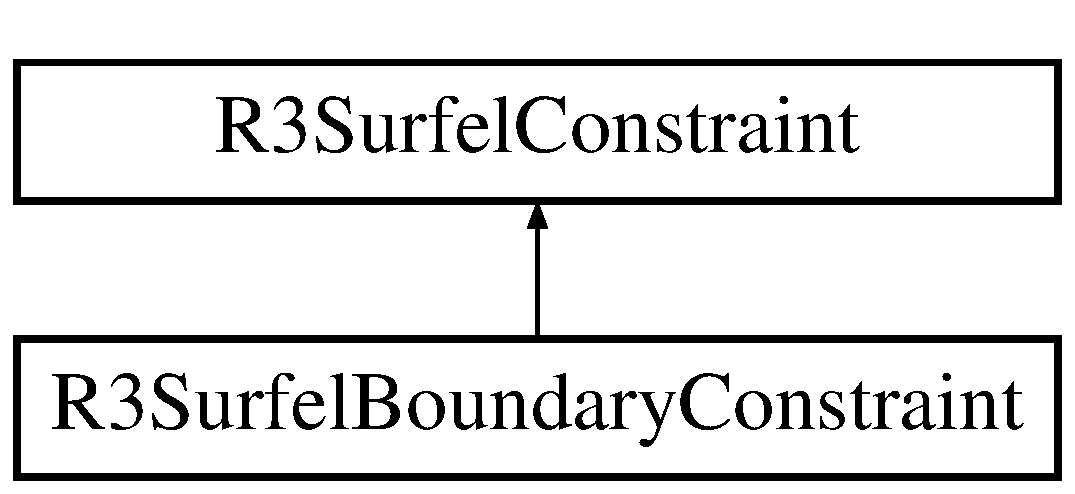
\includegraphics[height=2.000000cm]{class_r3_surfel_boundary_constraint}
\end{center}
\end{figure}
\subsection*{Public Member Functions}
\begin{DoxyCompactItemize}
\item 
{\bfseries R3\+Surfel\+Boundary\+Constraint} (R\+N\+Boolean include\+\_\+interior=T\+R\+UE, R\+N\+Boolean include\+\_\+border=F\+A\+L\+SE, R\+N\+Boolean include\+\_\+silhouette=F\+A\+L\+SE, R\+N\+Boolean include\+\_\+shadow=F\+A\+L\+SE)\hypertarget{class_r3_surfel_boundary_constraint_a1dfbd52c6ed90e92d1ab5d6719f44afe}{}\label{class_r3_surfel_boundary_constraint_a1dfbd52c6ed90e92d1ab5d6719f44afe}

\item 
virtual int {\bfseries Check} (const \hyperlink{class_r3_surfel_block}{R3\+Surfel\+Block} $\ast$block, const \hyperlink{class_r3_surfel}{R3\+Surfel} $\ast$surfel) const \hypertarget{class_r3_surfel_boundary_constraint_ae69e6f1836e1ac338a28b6c8f13fad25}{}\label{class_r3_surfel_boundary_constraint_ae69e6f1836e1ac338a28b6c8f13fad25}

\end{DoxyCompactItemize}


The documentation for this class was generated from the following files\+:\begin{DoxyCompactItemize}
\item 
R3\+Surfels/R3\+Surfel\+Constraint.\+h\item 
R3\+Surfels/R3\+Surfel\+Constraint.\+cpp\end{DoxyCompactItemize}

\hypertarget{class_r3_surfel_box_constraint}{}\section{R3\+Surfel\+Box\+Constraint Class Reference}
\label{class_r3_surfel_box_constraint}\index{R3\+Surfel\+Box\+Constraint@{R3\+Surfel\+Box\+Constraint}}
Inheritance diagram for R3\+Surfel\+Box\+Constraint\+:\begin{figure}[H]
\begin{center}
\leavevmode
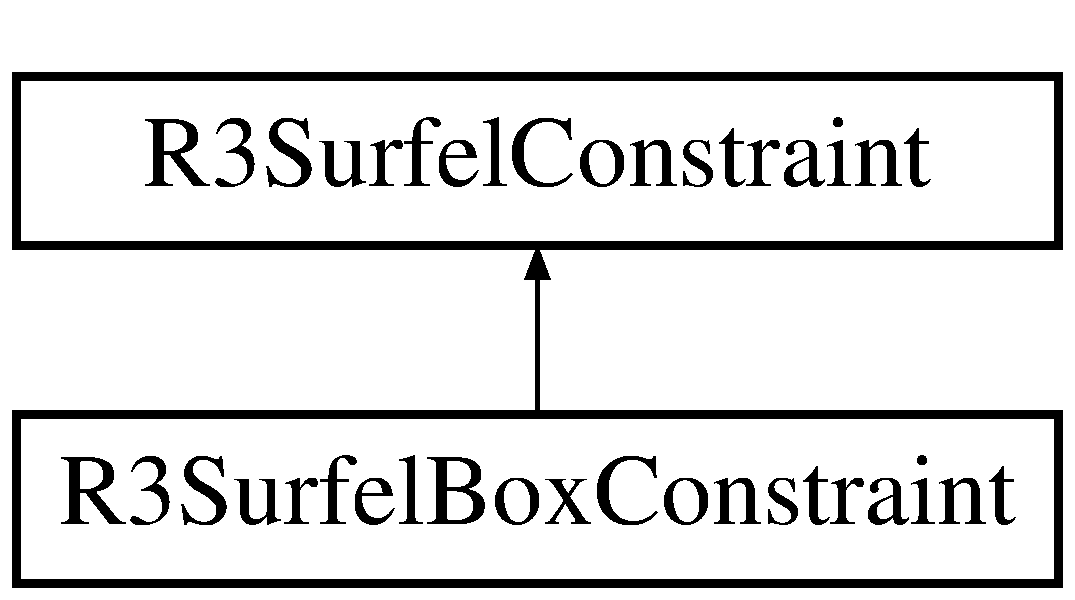
\includegraphics[height=2.000000cm]{class_r3_surfel_box_constraint}
\end{center}
\end{figure}
\subsection*{Public Member Functions}
\begin{DoxyCompactItemize}
\item 
{\bfseries R3\+Surfel\+Box\+Constraint} (const \hyperlink{class_r3_box}{R3\+Box} \&\hyperlink{structbox}{box})\hypertarget{class_r3_surfel_box_constraint_a5ec1fe2c5799d3e518ccc7032e80db0c}{}\label{class_r3_surfel_box_constraint_a5ec1fe2c5799d3e518ccc7032e80db0c}

\item 
virtual int {\bfseries Check} (const \hyperlink{class_r3_point}{R3\+Point} \&point) const \hypertarget{class_r3_surfel_box_constraint_ae3731306d61b3f2006e99ea9e36ef55e}{}\label{class_r3_surfel_box_constraint_ae3731306d61b3f2006e99ea9e36ef55e}

\item 
virtual int {\bfseries Check} (const \hyperlink{class_r3_box}{R3\+Box} \&\hyperlink{structbox}{box}) const \hypertarget{class_r3_surfel_box_constraint_ae9751bf2292546db9940411ca2e3ccd5}{}\label{class_r3_surfel_box_constraint_ae9751bf2292546db9940411ca2e3ccd5}

\end{DoxyCompactItemize}


The documentation for this class was generated from the following files\+:\begin{DoxyCompactItemize}
\item 
R3\+Surfels/R3\+Surfel\+Constraint.\+h\item 
R3\+Surfels/R3\+Surfel\+Constraint.\+cpp\end{DoxyCompactItemize}

\hypertarget{struct_r3_surfel_cluster}{}\section{R3\+Surfel\+Cluster Struct Reference}
\label{struct_r3_surfel_cluster}\index{R3\+Surfel\+Cluster@{R3\+Surfel\+Cluster}}
\subsection*{Public Attributes}
\begin{DoxyCompactItemize}
\item 
\hyperlink{struct_r3_surfel_cluster}{R3\+Surfel\+Cluster} $\ast$ {\bfseries parent}\hypertarget{struct_r3_surfel_cluster_acddf2e9ec9ccaf558ea954b345d30775}{}\label{struct_r3_surfel_cluster_acddf2e9ec9ccaf558ea954b345d30775}

\item 
\hyperlink{class_r_n_array}{R\+N\+Array}$<$ \hyperlink{class_r3_surfel_point}{R3\+Surfel\+Point} $\ast$ $>$ {\bfseries points}\hypertarget{struct_r3_surfel_cluster_aeb5bef2de1fa230f77f4e29ea71c436a}{}\label{struct_r3_surfel_cluster_aeb5bef2de1fa230f77f4e29ea71c436a}

\item 
\hyperlink{class_r3_box}{R3\+Box} {\bfseries bbox}\hypertarget{struct_r3_surfel_cluster_a2e2aa01e6179adb538f5e50b40eb3703}{}\label{struct_r3_surfel_cluster_a2e2aa01e6179adb538f5e50b40eb3703}

\item 
int {\bfseries id}\hypertarget{struct_r3_surfel_cluster_a63911c3e92e74bb5768878ebd90d624f}{}\label{struct_r3_surfel_cluster_a63911c3e92e74bb5768878ebd90d624f}

\end{DoxyCompactItemize}


The documentation for this struct was generated from the following file\+:\begin{DoxyCompactItemize}
\item 
R3\+Surfels/R3\+Surfel\+Utils.\+cpp\end{DoxyCompactItemize}

\hypertarget{struct_r3_surfel_cluster_pair}{}\section{R3\+Surfel\+Cluster\+Pair Struct Reference}
\label{struct_r3_surfel_cluster_pair}\index{R3\+Surfel\+Cluster\+Pair@{R3\+Surfel\+Cluster\+Pair}}
\subsection*{Public Attributes}
\begin{DoxyCompactItemize}
\item 
\hyperlink{struct_r3_surfel_cluster}{R3\+Surfel\+Cluster} $\ast$ {\bfseries clusters} \mbox{[}2\mbox{]}\hypertarget{struct_r3_surfel_cluster_pair_a9b0b45942d3a2c7abc0b060afe891d51}{}\label{struct_r3_surfel_cluster_pair_a9b0b45942d3a2c7abc0b060afe891d51}

\item 
R\+N\+Scalar {\bfseries similarity}\hypertarget{struct_r3_surfel_cluster_pair_a9940550ff8ff3f7734476adbc92d6eb4}{}\label{struct_r3_surfel_cluster_pair_a9940550ff8ff3f7734476adbc92d6eb4}

\end{DoxyCompactItemize}


The documentation for this struct was generated from the following file\+:\begin{DoxyCompactItemize}
\item 
R3\+Surfels/R3\+Surfel\+Utils.\+cpp\end{DoxyCompactItemize}

\hypertarget{class_r3_surfel_constraint}{}\section{R3\+Surfel\+Constraint Class Reference}
\label{class_r3_surfel_constraint}\index{R3\+Surfel\+Constraint@{R3\+Surfel\+Constraint}}
Inheritance diagram for R3\+Surfel\+Constraint\+:\begin{figure}[H]
\begin{center}
\leavevmode
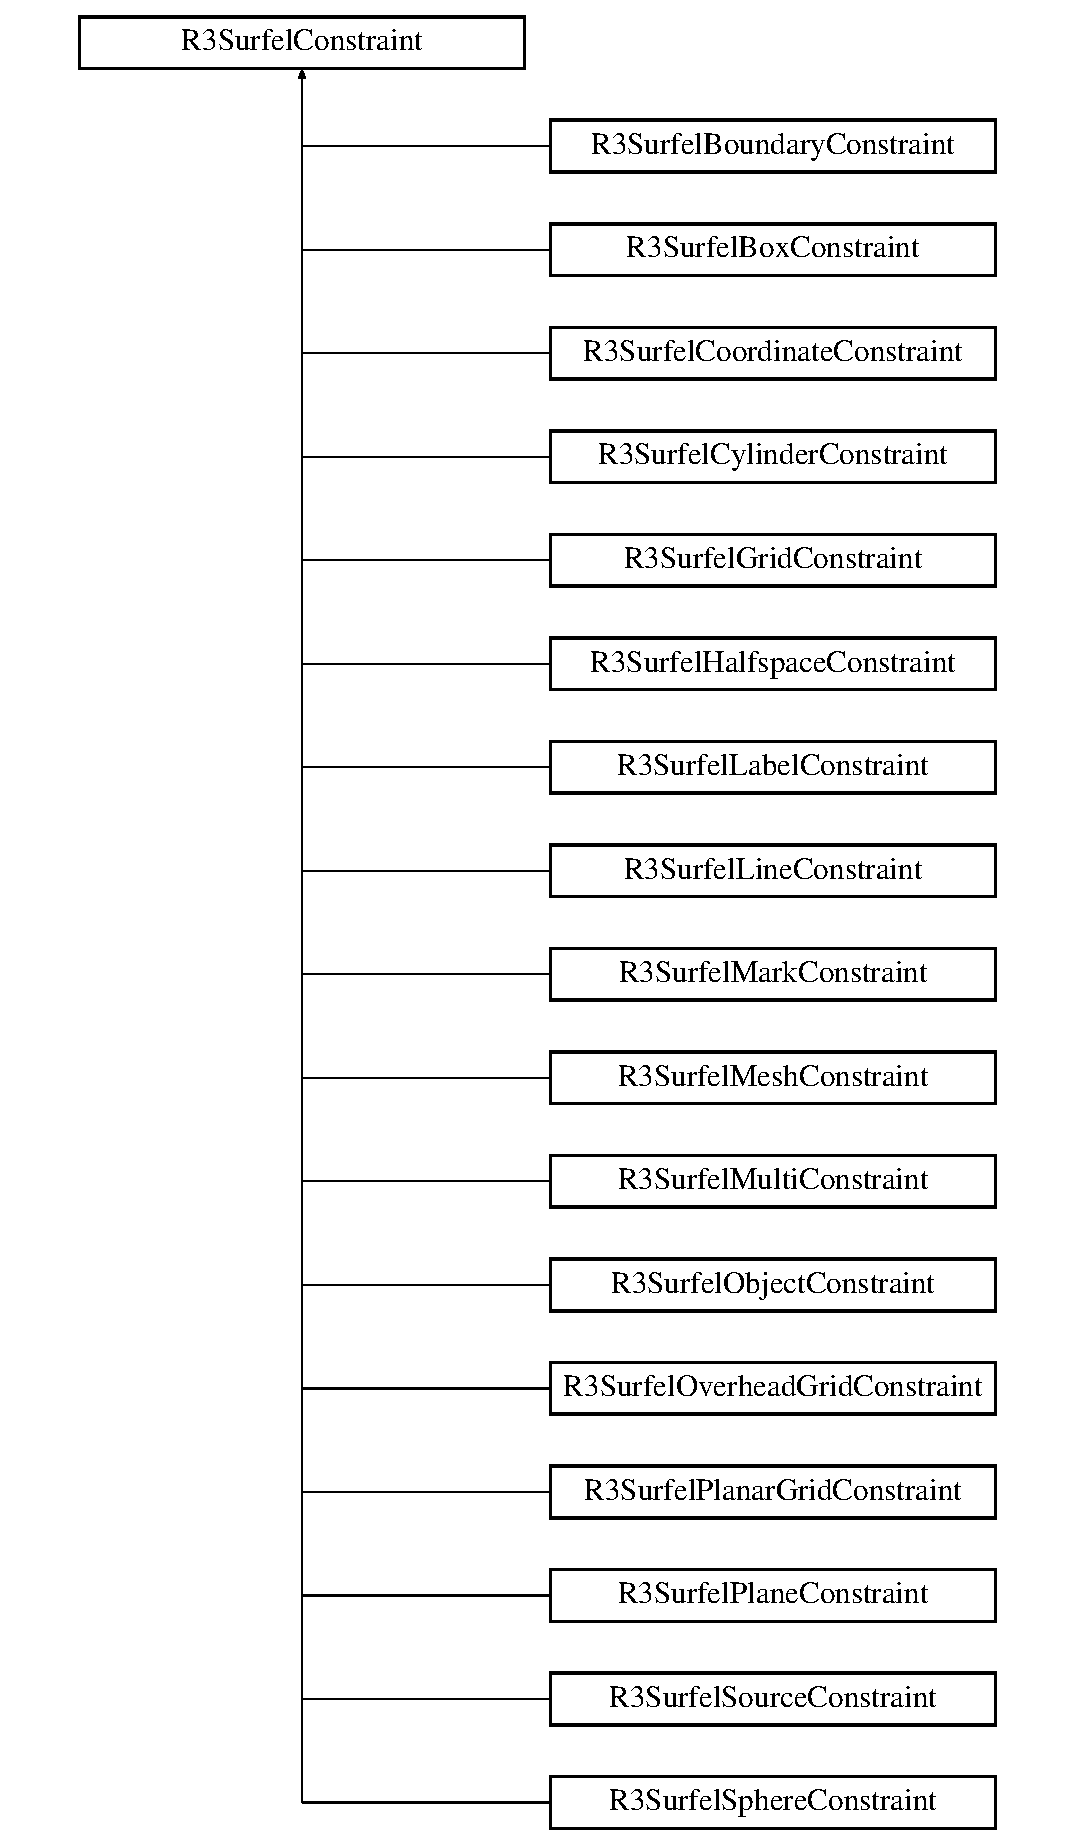
\includegraphics[height=12.000000cm]{class_r3_surfel_constraint}
\end{center}
\end{figure}
\subsection*{Public Member Functions}
\begin{DoxyCompactItemize}
\item 
virtual int {\bfseries Check} (const \hyperlink{class_r3_surfel_object}{R3\+Surfel\+Object} $\ast$object) const \hypertarget{class_r3_surfel_constraint_ada17b4eff1d7e1e0b20e4cb3922958e6}{}\label{class_r3_surfel_constraint_ada17b4eff1d7e1e0b20e4cb3922958e6}

\item 
virtual int {\bfseries Check} (const \hyperlink{class_r3_surfel_node}{R3\+Surfel\+Node} $\ast$node) const \hypertarget{class_r3_surfel_constraint_a5b81e7fb681cf2396544b62088b5571f}{}\label{class_r3_surfel_constraint_a5b81e7fb681cf2396544b62088b5571f}

\item 
virtual int {\bfseries Check} (const \hyperlink{class_r3_surfel_block}{R3\+Surfel\+Block} $\ast$block) const \hypertarget{class_r3_surfel_constraint_af4a15876be35993bf11c4bca287995af}{}\label{class_r3_surfel_constraint_af4a15876be35993bf11c4bca287995af}

\item 
virtual int {\bfseries Check} (const \hyperlink{class_r3_surfel_block}{R3\+Surfel\+Block} $\ast$block, const \hyperlink{class_r3_surfel}{R3\+Surfel} $\ast$surfel) const \hypertarget{class_r3_surfel_constraint_a4e7fda8cd9e795f18fbb7d9ff7b0a8ee}{}\label{class_r3_surfel_constraint_a4e7fda8cd9e795f18fbb7d9ff7b0a8ee}

\item 
virtual int {\bfseries Check} (const \hyperlink{class_r3_box}{R3\+Box} \&\hyperlink{structbox}{box}) const \hypertarget{class_r3_surfel_constraint_a50990acb5aa1007511352201a08cbef5}{}\label{class_r3_surfel_constraint_a50990acb5aa1007511352201a08cbef5}

\item 
virtual int {\bfseries Check} (const \hyperlink{class_r3_point}{R3\+Point} \&point) const \hypertarget{class_r3_surfel_constraint_ae050bee7798580b22a62007db618aa3e}{}\label{class_r3_surfel_constraint_ae050bee7798580b22a62007db618aa3e}

\end{DoxyCompactItemize}


The documentation for this class was generated from the following files\+:\begin{DoxyCompactItemize}
\item 
R3\+Surfels/R3\+Surfel\+Constraint.\+h\item 
R3\+Surfels/R3\+Surfel\+Constraint.\+cpp\end{DoxyCompactItemize}

\hypertarget{class_r3_surfel_coordinate_constraint}{}\section{R3\+Surfel\+Coordinate\+Constraint Class Reference}
\label{class_r3_surfel_coordinate_constraint}\index{R3\+Surfel\+Coordinate\+Constraint@{R3\+Surfel\+Coordinate\+Constraint}}
Inheritance diagram for R3\+Surfel\+Coordinate\+Constraint\+:\begin{figure}[H]
\begin{center}
\leavevmode
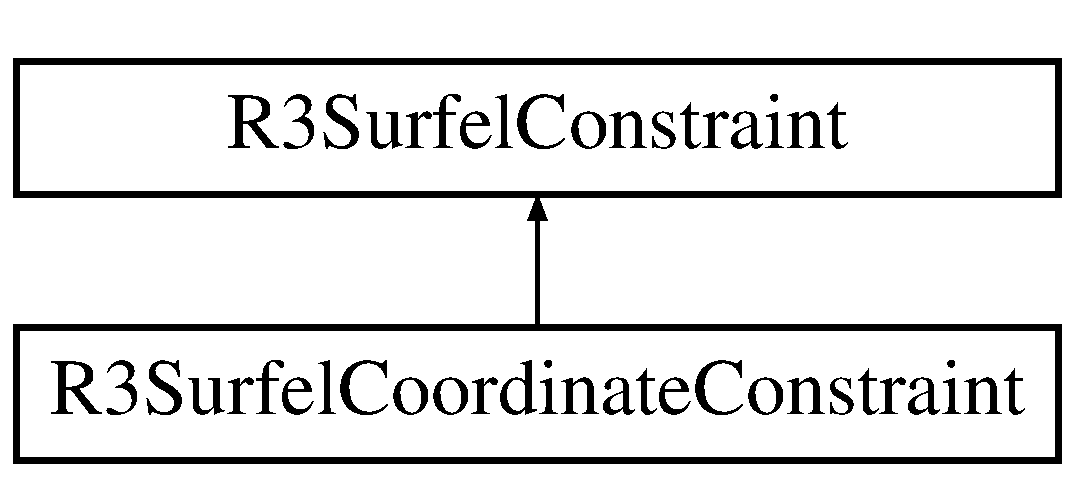
\includegraphics[height=2.000000cm]{class_r3_surfel_coordinate_constraint}
\end{center}
\end{figure}
\subsection*{Public Member Functions}
\begin{DoxyCompactItemize}
\item 
{\bfseries R3\+Surfel\+Coordinate\+Constraint} (R\+N\+Dimension dimension, const \hyperlink{class_r_n_interval}{R\+N\+Interval} \&interval)\hypertarget{class_r3_surfel_coordinate_constraint_a2ea8b4fd96b2ff8c4e28f07ec5423c8e}{}\label{class_r3_surfel_coordinate_constraint_a2ea8b4fd96b2ff8c4e28f07ec5423c8e}

\item 
virtual int {\bfseries Check} (const \hyperlink{class_r3_point}{R3\+Point} \&point) const \hypertarget{class_r3_surfel_coordinate_constraint_a00ffa7b6b9fe4d0f7ee57ce40eb3d856}{}\label{class_r3_surfel_coordinate_constraint_a00ffa7b6b9fe4d0f7ee57ce40eb3d856}

\item 
virtual int {\bfseries Check} (const \hyperlink{class_r3_box}{R3\+Box} \&\hyperlink{structbox}{box}) const \hypertarget{class_r3_surfel_coordinate_constraint_a04ce1992ed2c2b1c24926c2807c7e063}{}\label{class_r3_surfel_coordinate_constraint_a04ce1992ed2c2b1c24926c2807c7e063}

\end{DoxyCompactItemize}


The documentation for this class was generated from the following files\+:\begin{DoxyCompactItemize}
\item 
R3\+Surfels/R3\+Surfel\+Constraint.\+h\item 
R3\+Surfels/R3\+Surfel\+Constraint.\+cpp\end{DoxyCompactItemize}

\hypertarget{class_r3_surfel_cylinder_constraint}{}\section{R3\+Surfel\+Cylinder\+Constraint Class Reference}
\label{class_r3_surfel_cylinder_constraint}\index{R3\+Surfel\+Cylinder\+Constraint@{R3\+Surfel\+Cylinder\+Constraint}}
Inheritance diagram for R3\+Surfel\+Cylinder\+Constraint\+:\begin{figure}[H]
\begin{center}
\leavevmode
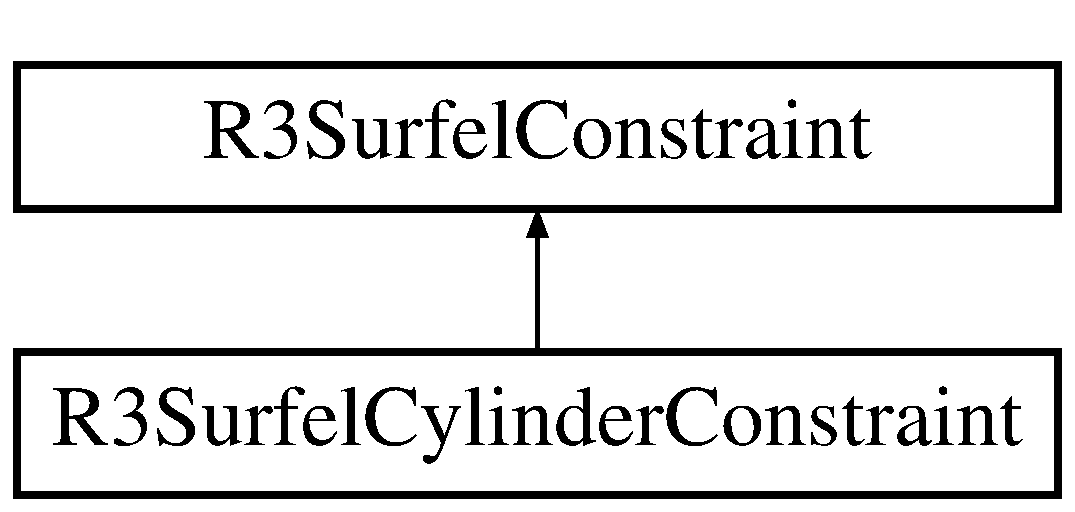
\includegraphics[height=2.000000cm]{class_r3_surfel_cylinder_constraint}
\end{center}
\end{figure}
\subsection*{Public Member Functions}
\begin{DoxyCompactItemize}
\item 
{\bfseries R3\+Surfel\+Cylinder\+Constraint} (const \hyperlink{class_r3_point}{R3\+Point} \&center, R\+N\+Length radius, R\+N\+Coord zmin=-\/F\+L\+T\+\_\+\+M\+AX, R\+N\+Coord zmax=F\+L\+T\+\_\+\+M\+AX)\hypertarget{class_r3_surfel_cylinder_constraint_a4826ed697d70393dd3a035e0b2506345}{}\label{class_r3_surfel_cylinder_constraint_a4826ed697d70393dd3a035e0b2506345}

\item 
virtual int {\bfseries Check} (const \hyperlink{class_r3_point}{R3\+Point} \&point) const \hypertarget{class_r3_surfel_cylinder_constraint_a33315cce4f05ce22f9dee3bf65aebac2}{}\label{class_r3_surfel_cylinder_constraint_a33315cce4f05ce22f9dee3bf65aebac2}

\item 
virtual int {\bfseries Check} (const \hyperlink{class_r3_box}{R3\+Box} \&\hyperlink{structbox}{box}) const \hypertarget{class_r3_surfel_cylinder_constraint_a6f81269f9f1d9b80cac708d767a8ecd2}{}\label{class_r3_surfel_cylinder_constraint_a6f81269f9f1d9b80cac708d767a8ecd2}

\end{DoxyCompactItemize}


The documentation for this class was generated from the following files\+:\begin{DoxyCompactItemize}
\item 
R3\+Surfels/R3\+Surfel\+Constraint.\+h\item 
R3\+Surfels/R3\+Surfel\+Constraint.\+cpp\end{DoxyCompactItemize}

\hypertarget{class_r3_surfel_database}{}\section{R3\+Surfel\+Database Class Reference}
\label{class_r3_surfel_database}\index{R3\+Surfel\+Database@{R3\+Surfel\+Database}}
\subsection*{Public Member Functions}
\begin{DoxyCompactItemize}
\item 
{\bfseries R3\+Surfel\+Database} (const \hyperlink{class_r3_surfel_database}{R3\+Surfel\+Database} \&database)\hypertarget{class_r3_surfel_database_af3a502b6dbe607b68c32720d3e05586c}{}\label{class_r3_surfel_database_af3a502b6dbe607b68c32720d3e05586c}

\item 
int {\bfseries N\+Surfels} (void) const \hypertarget{class_r3_surfel_database_afcee4c881ee31385563f451e42a63d69}{}\label{class_r3_surfel_database_afcee4c881ee31385563f451e42a63d69}

\item 
const char $\ast$ {\bfseries Name} (void) const \hypertarget{class_r3_surfel_database_a170144e6a8df8643e0f8ca4daebe65ed}{}\label{class_r3_surfel_database_a170144e6a8df8643e0f8ca4daebe65ed}

\item 
const \hyperlink{class_r3_box}{R3\+Box} \& {\bfseries B\+Box} (void) const \hypertarget{class_r3_surfel_database_ad8540f6fdf7b224c6dae5ce492361394}{}\label{class_r3_surfel_database_ad8540f6fdf7b224c6dae5ce492361394}

\item 
\hyperlink{class_r3_point}{R3\+Point} {\bfseries Centroid} (void) const \hypertarget{class_r3_surfel_database_a2f752122a68d6c5bd11c2593e913d8f0}{}\label{class_r3_surfel_database_a2f752122a68d6c5bd11c2593e913d8f0}

\item 
\hyperlink{class_r3_surfel_tree}{R3\+Surfel\+Tree} $\ast$ {\bfseries Tree} (void) const \hypertarget{class_r3_surfel_database_ab4ed15cd77c435284554c19cc18e0a71}{}\label{class_r3_surfel_database_ab4ed15cd77c435284554c19cc18e0a71}

\item 
int {\bfseries N\+Blocks} (void) const \hypertarget{class_r3_surfel_database_af8e49fc3f6df3fe1f2c2dfd807da9708}{}\label{class_r3_surfel_database_af8e49fc3f6df3fe1f2c2dfd807da9708}

\item 
\hyperlink{class_r3_surfel_block}{R3\+Surfel\+Block} $\ast$ {\bfseries Block} (int k) const \hypertarget{class_r3_surfel_database_aef473e7ec542c39680ffde2d49b0c754}{}\label{class_r3_surfel_database_aef473e7ec542c39680ffde2d49b0c754}

\item 
void {\bfseries Set\+Name} (const char $\ast$name)\hypertarget{class_r3_surfel_database_afce39626c6469ac29409e91c80d2b3af}{}\label{class_r3_surfel_database_afce39626c6469ac29409e91c80d2b3af}

\item 
virtual void {\bfseries Insert\+Block} (\hyperlink{class_r3_surfel_block}{R3\+Surfel\+Block} $\ast$block)\hypertarget{class_r3_surfel_database_ae16276217de50da8cb8834b8ee42b851}{}\label{class_r3_surfel_database_ae16276217de50da8cb8834b8ee42b851}

\item 
virtual void {\bfseries Remove\+Block} (\hyperlink{class_r3_surfel_block}{R3\+Surfel\+Block} $\ast$block)\hypertarget{class_r3_surfel_database_ac5973d807291c1d495fe30d42121868b}{}\label{class_r3_surfel_database_ac5973d807291c1d495fe30d42121868b}

\item 
virtual void {\bfseries Remove\+And\+Delete\+Block} (\hyperlink{class_r3_surfel_block}{R3\+Surfel\+Block} $\ast$block)\hypertarget{class_r3_surfel_database_a8e51d7c748adfc8a6a9a787bc43227de}{}\label{class_r3_surfel_database_a8e51d7c748adfc8a6a9a787bc43227de}

\item 
virtual int {\bfseries Insert\+Subset\+Blocks} (\hyperlink{class_r3_surfel_block}{R3\+Surfel\+Block} $\ast$block, const \hyperlink{class_r_n_array}{R\+N\+Array}$<$ const \hyperlink{class_r3_surfel}{R3\+Surfel} $\ast$ $>$ \&subsetA, const \hyperlink{class_r_n_array}{R\+N\+Array}$<$ const \hyperlink{class_r3_surfel}{R3\+Surfel} $\ast$ $>$ \&subsetB, \hyperlink{class_r3_surfel_block}{R3\+Surfel\+Block} $\ast$$\ast$blockA, \hyperlink{class_r3_surfel_block}{R3\+Surfel\+Block} $\ast$$\ast$blockB)\hypertarget{class_r3_surfel_database_a7dae5ce0aed2403fe9301bd5018e7d45}{}\label{class_r3_surfel_database_a7dae5ce0aed2403fe9301bd5018e7d45}

\item 
void {\bfseries Set\+Marks} (R\+N\+Boolean mark=T\+R\+UE)\hypertarget{class_r3_surfel_database_a23bc379821a9350889b4f3259f1989a7}{}\label{class_r3_surfel_database_a23bc379821a9350889b4f3259f1989a7}

\item 
int {\bfseries Read\+Block} (\hyperlink{class_r3_surfel_block}{R3\+Surfel\+Block} $\ast$block)\hypertarget{class_r3_surfel_database_a1c773b91bbc66bc898b32bbe75675919}{}\label{class_r3_surfel_database_a1c773b91bbc66bc898b32bbe75675919}

\item 
int {\bfseries Release\+Block} (\hyperlink{class_r3_surfel_block}{R3\+Surfel\+Block} $\ast$block)\hypertarget{class_r3_surfel_database_a0b38b20cdd261c708bd974551a56b63b}{}\label{class_r3_surfel_database_a0b38b20cdd261c708bd974551a56b63b}

\item 
int {\bfseries Sync\+Block} (\hyperlink{class_r3_surfel_block}{R3\+Surfel\+Block} $\ast$block)\hypertarget{class_r3_surfel_database_a4eafc8317e3efccd564f0b9946ee8915}{}\label{class_r3_surfel_database_a4eafc8317e3efccd564f0b9946ee8915}

\item 
R\+N\+Boolean {\bfseries Is\+Block\+Resident} (\hyperlink{class_r3_surfel_block}{R3\+Surfel\+Block} $\ast$block) const \hypertarget{class_r3_surfel_database_a2a0d5ec9d161c6eea35d73d46a22c62e}{}\label{class_r3_surfel_database_a2a0d5ec9d161c6eea35d73d46a22c62e}

\item 
unsigned long {\bfseries Resident\+Surfels} (void) const \hypertarget{class_r3_surfel_database_a2d804d7f7a5af0955a9b9b43c66d5710}{}\label{class_r3_surfel_database_a2d804d7f7a5af0955a9b9b43c66d5710}

\item 
virtual int {\bfseries Open\+File} (const char $\ast$filename, const char $\ast$rwaccess=N\+U\+LL)\hypertarget{class_r3_surfel_database_a4a976c018f6706ef97432fdfa15ae1a1}{}\label{class_r3_surfel_database_a4a976c018f6706ef97432fdfa15ae1a1}

\item 
virtual int {\bfseries Sync\+File} (void)\hypertarget{class_r3_surfel_database_a76932725db5356b6446a75e2d8fdb842}{}\label{class_r3_surfel_database_a76932725db5356b6446a75e2d8fdb842}

\item 
virtual int {\bfseries Close\+File} (void)\hypertarget{class_r3_surfel_database_a142b373a97b84aca4a0ba77a3e1483bd}{}\label{class_r3_surfel_database_a142b373a97b84aca4a0ba77a3e1483bd}

\item 
virtual R\+N\+Boolean {\bfseries Is\+Open} (void) const \hypertarget{class_r3_surfel_database_a05a768f388d44804ef80d88ade70bf8b}{}\label{class_r3_surfel_database_a05a768f388d44804ef80d88ade70bf8b}

\item 
virtual int {\bfseries Read\+File} (const char $\ast$filename)\hypertarget{class_r3_surfel_database_a24337bc7e9f6a21de2dc1f8eb18b0be4}{}\label{class_r3_surfel_database_a24337bc7e9f6a21de2dc1f8eb18b0be4}

\item 
virtual int {\bfseries Write\+File} (const char $\ast$filename) const \hypertarget{class_r3_surfel_database_aa65bd789df04eb8404e0d705088b3fcc}{}\label{class_r3_surfel_database_aa65bd789df04eb8404e0d705088b3fcc}

\item 
virtual void {\bfseries Draw} (\hyperlink{class_r_n_flags}{R\+N\+Flags} flags=R3\+\_\+\+S\+U\+R\+F\+E\+L\+\_\+\+D\+E\+F\+A\+U\+L\+T\+\_\+\+D\+R\+A\+W\+\_\+\+F\+L\+A\+GS) const \hypertarget{class_r3_surfel_database_a697607241ec3415fc85c7a5f2054c3f8}{}\label{class_r3_surfel_database_a697607241ec3415fc85c7a5f2054c3f8}

\item 
virtual void {\bfseries Print} (F\+I\+LE $\ast$fp=N\+U\+LL, const char $\ast$prefix=N\+U\+LL, const char $\ast$suffix=N\+U\+LL) const \hypertarget{class_r3_surfel_database_a94a9c9e4f331feba5a58830c95efc4f2}{}\label{class_r3_surfel_database_a94a9c9e4f331feba5a58830c95efc4f2}

\end{DoxyCompactItemize}
\subsection*{Protected Member Functions}
\begin{DoxyCompactItemize}
\item 
virtual int {\bfseries Internal\+Read\+Block} (\hyperlink{class_r3_surfel_block}{R3\+Surfel\+Block} $\ast$block)\hypertarget{class_r3_surfel_database_af4d87914f40606bd19d52c0af1d2cbaa}{}\label{class_r3_surfel_database_af4d87914f40606bd19d52c0af1d2cbaa}

\item 
virtual int {\bfseries Internal\+Release\+Block} (\hyperlink{class_r3_surfel_block}{R3\+Surfel\+Block} $\ast$block)\hypertarget{class_r3_surfel_database_a039fd684c35cc111512b527dc4742cb7}{}\label{class_r3_surfel_database_a039fd684c35cc111512b527dc4742cb7}

\item 
virtual int {\bfseries Internal\+Sync\+Block} (\hyperlink{class_r3_surfel_block}{R3\+Surfel\+Block} $\ast$block)\hypertarget{class_r3_surfel_database_a702ce175a88d88989d8f33e0418c51e6}{}\label{class_r3_surfel_database_a702ce175a88d88989d8f33e0418c51e6}

\item 
virtual int {\bfseries Write\+Header} (F\+I\+LE $\ast$fp, int swap\+\_\+endian)\hypertarget{class_r3_surfel_database_ab517443be336039648bc9caf2732be97}{}\label{class_r3_surfel_database_ab517443be336039648bc9caf2732be97}

\end{DoxyCompactItemize}
\subsection*{Protected Attributes}
\begin{DoxyCompactItemize}
\item 
F\+I\+LE $\ast$ {\bfseries fp}\hypertarget{class_r3_surfel_database_a3989dcfef3c4b81f7cb51388e44b7cf7}{}\label{class_r3_surfel_database_a3989dcfef3c4b81f7cb51388e44b7cf7}

\item 
char $\ast$ {\bfseries filename}\hypertarget{class_r3_surfel_database_adcab62eb583e8b42d8712c679f6bd3b0}{}\label{class_r3_surfel_database_adcab62eb583e8b42d8712c679f6bd3b0}

\item 
char $\ast$ {\bfseries rwaccess}\hypertarget{class_r3_surfel_database_a75c7d17ac62b8f7352e34e7138676f85}{}\label{class_r3_surfel_database_a75c7d17ac62b8f7352e34e7138676f85}

\item 
unsigned int {\bfseries major\+\_\+version}\hypertarget{class_r3_surfel_database_a66dd461499c48f418768e4017a2b25aa}{}\label{class_r3_surfel_database_a66dd461499c48f418768e4017a2b25aa}

\item 
unsigned int {\bfseries minor\+\_\+version}\hypertarget{class_r3_surfel_database_ac60a4adf7e59272520fd77da27ab2ac4}{}\label{class_r3_surfel_database_ac60a4adf7e59272520fd77da27ab2ac4}

\item 
unsigned int {\bfseries swap\+\_\+endian}\hypertarget{class_r3_surfel_database_afa765040d282c03f801c180928fa9410}{}\label{class_r3_surfel_database_afa765040d282c03f801c180928fa9410}

\item 
unsigned long long {\bfseries file\+\_\+blocks\+\_\+offset}\hypertarget{class_r3_surfel_database_a3d6ff43118f72e1db3df15a4d7518470}{}\label{class_r3_surfel_database_a3d6ff43118f72e1db3df15a4d7518470}

\item 
unsigned int {\bfseries file\+\_\+blocks\+\_\+count}\hypertarget{class_r3_surfel_database_af5351798bb27bc53418118b7db78158b}{}\label{class_r3_surfel_database_af5351798bb27bc53418118b7db78158b}

\item 
\hyperlink{class_r_n_array}{R\+N\+Array}$<$ \hyperlink{class_r3_surfel_block}{R3\+Surfel\+Block} $\ast$ $>$ {\bfseries blocks}\hypertarget{class_r3_surfel_database_a1e5843a85559f72ce02385cb179faefc}{}\label{class_r3_surfel_database_a1e5843a85559f72ce02385cb179faefc}

\item 
int {\bfseries nsurfels}\hypertarget{class_r3_surfel_database_a270de0a7e95e3cb909e67eb8d0623d66}{}\label{class_r3_surfel_database_a270de0a7e95e3cb909e67eb8d0623d66}

\item 
\hyperlink{class_r3_box}{R3\+Box} {\bfseries bbox}\hypertarget{class_r3_surfel_database_a9a9dca95eabcb6396d656e480272a745}{}\label{class_r3_surfel_database_a9a9dca95eabcb6396d656e480272a745}

\item 
char $\ast$ {\bfseries name}\hypertarget{class_r3_surfel_database_aa4e12e1f121cfe3f1c9c8b5507ee3b39}{}\label{class_r3_surfel_database_aa4e12e1f121cfe3f1c9c8b5507ee3b39}

\item 
\hyperlink{class_r3_surfel_tree}{R3\+Surfel\+Tree} $\ast$ {\bfseries tree}\hypertarget{class_r3_surfel_database_aaec3b65fb3a767a03a116117413c8d9b}{}\label{class_r3_surfel_database_aaec3b65fb3a767a03a116117413c8d9b}

\item 
unsigned long {\bfseries resident\+\_\+surfels}\hypertarget{class_r3_surfel_database_a3593f8e45d057f1d0d87e390ad91d5bf}{}\label{class_r3_surfel_database_a3593f8e45d057f1d0d87e390ad91d5bf}

\end{DoxyCompactItemize}
\subsection*{Friends}
\begin{DoxyCompactItemize}
\item 
class {\bfseries R3\+Surfel\+Tree}\hypertarget{class_r3_surfel_database_afe80cf8b46036b5125f7c9280809ed48}{}\label{class_r3_surfel_database_afe80cf8b46036b5125f7c9280809ed48}

\end{DoxyCompactItemize}


The documentation for this class was generated from the following files\+:\begin{DoxyCompactItemize}
\item 
R3\+Surfels/R3\+Surfel\+Database.\+h\item 
R3\+Surfels/R3\+Surfel\+Database.\+cpp\end{DoxyCompactItemize}

\hypertarget{class_r3_surfel_feature}{}\section{R3\+Surfel\+Feature Class Reference}
\label{class_r3_surfel_feature}\index{R3\+Surfel\+Feature@{R3\+Surfel\+Feature}}
Inheritance diagram for R3\+Surfel\+Feature\+:\begin{figure}[H]
\begin{center}
\leavevmode
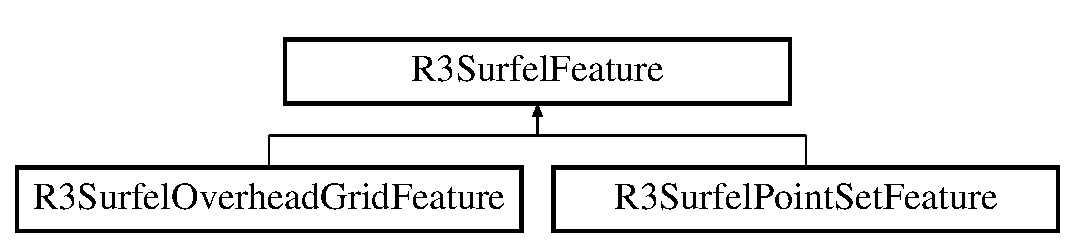
\includegraphics[height=2.000000cm]{class_r3_surfel_feature}
\end{center}
\end{figure}
\subsection*{Public Member Functions}
\begin{DoxyCompactItemize}
\item 
{\bfseries R3\+Surfel\+Feature} (const char $\ast$name=N\+U\+LL, R\+N\+Scalar minimum=-\/F\+L\+T\+\_\+\+M\+AX, R\+N\+Scalar maximum=F\+L\+T\+\_\+\+M\+AX, R\+N\+Scalar weight=1)\hypertarget{class_r3_surfel_feature_a029ddf68205af4fa97395025c45654ef}{}\label{class_r3_surfel_feature_a029ddf68205af4fa97395025c45654ef}

\item 
{\bfseries R3\+Surfel\+Feature} (const \hyperlink{class_r3_surfel_feature}{R3\+Surfel\+Feature} \&feature)\hypertarget{class_r3_surfel_feature_a918622779869655d8d855889d84f768b}{}\label{class_r3_surfel_feature_a918622779869655d8d855889d84f768b}

\item 
\hyperlink{class_r3_surfel_scene}{R3\+Surfel\+Scene} $\ast$ {\bfseries Scene} (void) const \hypertarget{class_r3_surfel_feature_a0221b0b9e0d8f9d9de003453f5f4fb89}{}\label{class_r3_surfel_feature_a0221b0b9e0d8f9d9de003453f5f4fb89}

\item 
int {\bfseries Scene\+Index} (void) const \hypertarget{class_r3_surfel_feature_a4c4167e2eaee028883a7d99640ca8592}{}\label{class_r3_surfel_feature_a4c4167e2eaee028883a7d99640ca8592}

\item 
const char $\ast$ {\bfseries Name} (void) const \hypertarget{class_r3_surfel_feature_a392c65e8d9dc2e7370b712e724a9baa1}{}\label{class_r3_surfel_feature_a392c65e8d9dc2e7370b712e724a9baa1}

\item 
const \hyperlink{class_r_n_interval}{R\+N\+Interval} \& {\bfseries Range} (void) const \hypertarget{class_r3_surfel_feature_ae0a6115e3acdff2c77a318d12a2e645f}{}\label{class_r3_surfel_feature_ae0a6115e3acdff2c77a318d12a2e645f}

\item 
R\+N\+Scalar {\bfseries Minimum} (void) const \hypertarget{class_r3_surfel_feature_a56fa29ddf4496106b9819d68a1d39e99}{}\label{class_r3_surfel_feature_a56fa29ddf4496106b9819d68a1d39e99}

\item 
R\+N\+Scalar {\bfseries Maximum} (void) const \hypertarget{class_r3_surfel_feature_a5dfcbf0c0bcc73c97b5fc3e960b05269}{}\label{class_r3_surfel_feature_a5dfcbf0c0bcc73c97b5fc3e960b05269}

\item 
R\+N\+Scalar {\bfseries Weight} (void) const \hypertarget{class_r3_surfel_feature_a89e1c27364b98b89009e72e549b9261a}{}\label{class_r3_surfel_feature_a89e1c27364b98b89009e72e549b9261a}

\item 
virtual int {\bfseries Type} (void) const \hypertarget{class_r3_surfel_feature_ae7763c09c37c422f9e5e28481ce3e542}{}\label{class_r3_surfel_feature_ae7763c09c37c422f9e5e28481ce3e542}

\item 
void $\ast$ {\bfseries Data} (void) const \hypertarget{class_r3_surfel_feature_a6d2baba218003058d2f7a21490c93ea2}{}\label{class_r3_surfel_feature_a6d2baba218003058d2f7a21490c93ea2}

\item 
void {\bfseries Set\+Name} (const char $\ast$name)\hypertarget{class_r3_surfel_feature_adf9b0381db158f9aae6858357607ba84}{}\label{class_r3_surfel_feature_adf9b0381db158f9aae6858357607ba84}

\item 
virtual void {\bfseries Set\+Range} (const \hyperlink{class_r_n_interval}{R\+N\+Interval} \&range)\hypertarget{class_r3_surfel_feature_af46dfd154f0a792f202948238c0c504c}{}\label{class_r3_surfel_feature_af46dfd154f0a792f202948238c0c504c}

\item 
virtual void {\bfseries Set\+Range} (R\+N\+Scalar minimum, R\+N\+Scalar maximum)\hypertarget{class_r3_surfel_feature_ad9b298e35f4375e9da94e839b5457143}{}\label{class_r3_surfel_feature_ad9b298e35f4375e9da94e839b5457143}

\item 
virtual void {\bfseries Set\+Minimum} (R\+N\+Scalar minimum)\hypertarget{class_r3_surfel_feature_aabf0524e4441c2d12626f2bfad398ee6}{}\label{class_r3_surfel_feature_aabf0524e4441c2d12626f2bfad398ee6}

\item 
virtual void {\bfseries Set\+Maximum} (R\+N\+Scalar maximum)\hypertarget{class_r3_surfel_feature_a6e9fc7a69072ba80f33f40df98626c22}{}\label{class_r3_surfel_feature_a6e9fc7a69072ba80f33f40df98626c22}

\item 
virtual void {\bfseries Set\+Weight} (R\+N\+Scalar weight)\hypertarget{class_r3_surfel_feature_a7392743c3193895d8ccba5f453b1b034}{}\label{class_r3_surfel_feature_a7392743c3193895d8ccba5f453b1b034}

\item 
virtual void {\bfseries Set\+Data} (void $\ast$data)\hypertarget{class_r3_surfel_feature_a41420480903d487ab057be566811a451}{}\label{class_r3_surfel_feature_a41420480903d487ab057be566811a451}

\item 
virtual int {\bfseries Update\+Feature\+Vector} (\hyperlink{class_r3_surfel_object}{R3\+Surfel\+Object} $\ast$object, \hyperlink{class_r3_surfel_feature_vector}{R3\+Surfel\+Feature\+Vector} \&vector) const \hypertarget{class_r3_surfel_feature_af2ebf6ba16bbccab4d0fcc68a5a4fb10}{}\label{class_r3_surfel_feature_af2ebf6ba16bbccab4d0fcc68a5a4fb10}

\item 
virtual void {\bfseries Print} (F\+I\+LE $\ast$fp=N\+U\+LL, const char $\ast$prefix=N\+U\+LL, const char $\ast$suffix=N\+U\+LL) const \hypertarget{class_r3_surfel_feature_acfe64c92a31afe0033fd1f0cede7d91e}{}\label{class_r3_surfel_feature_acfe64c92a31afe0033fd1f0cede7d91e}

\end{DoxyCompactItemize}
\subsection*{Friends}
\begin{DoxyCompactItemize}
\item 
class {\bfseries R3\+Surfel\+Scene}\hypertarget{class_r3_surfel_feature_af9bb32c0eac7d1d54787bbc6b44586b6}{}\label{class_r3_surfel_feature_af9bb32c0eac7d1d54787bbc6b44586b6}

\end{DoxyCompactItemize}


The documentation for this class was generated from the following files\+:\begin{DoxyCompactItemize}
\item 
R3\+Surfels/R3\+Surfel\+Feature.\+h\item 
R3\+Surfels/R3\+Surfel\+Feature.\+cpp\end{DoxyCompactItemize}

\hypertarget{class_r3_surfel_feature_set}{}\section{R3\+Surfel\+Feature\+Set Class Reference}
\label{class_r3_surfel_feature_set}\index{R3\+Surfel\+Feature\+Set@{R3\+Surfel\+Feature\+Set}}
\subsection*{Public Member Functions}
\begin{DoxyCompactItemize}
\item 
{\bfseries R3\+Surfel\+Feature\+Set} (const \hyperlink{class_r3_surfel_feature_set}{R3\+Surfel\+Feature\+Set} \&set)\hypertarget{class_r3_surfel_feature_set_adddbe3efa10dad77fe0e0c8a59464708}{}\label{class_r3_surfel_feature_set_adddbe3efa10dad77fe0e0c8a59464708}

\item 
int {\bfseries N\+Features} (void) const \hypertarget{class_r3_surfel_feature_set_aa525db28d564c08df6d88ba2a398ef13}{}\label{class_r3_surfel_feature_set_aa525db28d564c08df6d88ba2a398ef13}

\item 
\hyperlink{class_r3_surfel_feature}{R3\+Surfel\+Feature} $\ast$ {\bfseries Feature} (int k) const \hypertarget{class_r3_surfel_feature_set_ab47c50218a0990d104b888f16340e8b8}{}\label{class_r3_surfel_feature_set_ab47c50218a0990d104b888f16340e8b8}

\item 
\hyperlink{class_r3_surfel_feature}{R3\+Surfel\+Feature} $\ast$ {\bfseries operator\mbox{[}$\,$\mbox{]}} (int k) const \hypertarget{class_r3_surfel_feature_set_a4057524060a95493e41f130e6c21c86c}{}\label{class_r3_surfel_feature_set_a4057524060a95493e41f130e6c21c86c}

\item 
virtual void {\bfseries Insert\+Feature} (\hyperlink{class_r3_surfel_feature}{R3\+Surfel\+Feature} $\ast$feature)\hypertarget{class_r3_surfel_feature_set_abd8ebd244566e1436db16f05ef5340ab}{}\label{class_r3_surfel_feature_set_abd8ebd244566e1436db16f05ef5340ab}

\item 
virtual void {\bfseries Remove\+Feature} (\hyperlink{class_r3_surfel_feature}{R3\+Surfel\+Feature} $\ast$feature)\hypertarget{class_r3_surfel_feature_set_aaa41521cd85d56af7c596dbd3d2af526}{}\label{class_r3_surfel_feature_set_aaa41521cd85d56af7c596dbd3d2af526}

\item 
virtual void {\bfseries Remove\+Feature} (int k)\hypertarget{class_r3_surfel_feature_set_a40e3b4d95364a7986217d73a3ce8b481}{}\label{class_r3_surfel_feature_set_a40e3b4d95364a7986217d73a3ce8b481}

\item 
virtual void {\bfseries Empty} (void)\hypertarget{class_r3_surfel_feature_set_a2ba69597c212ee87f04527f06d11db04}{}\label{class_r3_surfel_feature_set_a2ba69597c212ee87f04527f06d11db04}

\item 
virtual void {\bfseries Print} (F\+I\+LE $\ast$fp=N\+U\+LL, const char $\ast$prefix=N\+U\+LL, const char $\ast$suffix=N\+U\+LL) const \hypertarget{class_r3_surfel_feature_set_af33ac7049f518399ecda0d8933160d64}{}\label{class_r3_surfel_feature_set_af33ac7049f518399ecda0d8933160d64}

\end{DoxyCompactItemize}


The documentation for this class was generated from the following files\+:\begin{DoxyCompactItemize}
\item 
R3\+Surfels/R3\+Surfel\+Feature\+Set.\+h\item 
R3\+Surfels/R3\+Surfel\+Feature\+Set.\+cpp\end{DoxyCompactItemize}

\hypertarget{class_r3_surfel_feature_vector}{}\section{R3\+Surfel\+Feature\+Vector Class Reference}
\label{class_r3_surfel_feature_vector}\index{R3\+Surfel\+Feature\+Vector@{R3\+Surfel\+Feature\+Vector}}
\subsection*{Public Member Functions}
\begin{DoxyCompactItemize}
\item 
{\bfseries R3\+Surfel\+Feature\+Vector} (int nvalues=0)\hypertarget{class_r3_surfel_feature_vector_aee3b6c306e9c9bbbb0ce590dffea5a0a}{}\label{class_r3_surfel_feature_vector_aee3b6c306e9c9bbbb0ce590dffea5a0a}

\item 
{\bfseries R3\+Surfel\+Feature\+Vector} (const \hyperlink{class_r3_surfel_feature_vector}{R3\+Surfel\+Feature\+Vector} \&vector)\hypertarget{class_r3_surfel_feature_vector_a18ea0c4805eafdf629959736dc810789}{}\label{class_r3_surfel_feature_vector_a18ea0c4805eafdf629959736dc810789}

\item 
int {\bfseries N\+Values} (void) const \hypertarget{class_r3_surfel_feature_vector_a790ba6798718202f0a2ef0420c05708f}{}\label{class_r3_surfel_feature_vector_a790ba6798718202f0a2ef0420c05708f}

\item 
R\+N\+Scalar {\bfseries Value} (int k) const \hypertarget{class_r3_surfel_feature_vector_ad369ddb0340023a479f69a82266b9f01}{}\label{class_r3_surfel_feature_vector_ad369ddb0340023a479f69a82266b9f01}

\item 
R\+N\+Scalar {\bfseries operator\mbox{[}$\,$\mbox{]}} (int k) const \hypertarget{class_r3_surfel_feature_vector_afeca7dc25cbfa427483b28cba537bc25}{}\label{class_r3_surfel_feature_vector_afeca7dc25cbfa427483b28cba537bc25}

\item 
\hyperlink{class_r3_surfel_feature_vector}{R3\+Surfel\+Feature\+Vector} \& {\bfseries operator=} (const \hyperlink{class_r3_surfel_feature_vector}{R3\+Surfel\+Feature\+Vector} \&vector)\hypertarget{class_r3_surfel_feature_vector_a747f16ad4203e39deaf6149a2f2a6843}{}\label{class_r3_surfel_feature_vector_a747f16ad4203e39deaf6149a2f2a6843}

\item 
\hyperlink{class_r3_surfel_feature_vector}{R3\+Surfel\+Feature\+Vector} \& {\bfseries operator+=} (const \hyperlink{class_r3_surfel_feature_vector}{R3\+Surfel\+Feature\+Vector} \&vector)\hypertarget{class_r3_surfel_feature_vector_ab3ec3751f83f911e6c1c22b317e3e760}{}\label{class_r3_surfel_feature_vector_ab3ec3751f83f911e6c1c22b317e3e760}

\item 
\hyperlink{class_r3_surfel_feature_vector}{R3\+Surfel\+Feature\+Vector} \& {\bfseries operator-\/=} (const \hyperlink{class_r3_surfel_feature_vector}{R3\+Surfel\+Feature\+Vector} \&vector)\hypertarget{class_r3_surfel_feature_vector_a428ab09083dff2929ee2c7c24348ec61}{}\label{class_r3_surfel_feature_vector_a428ab09083dff2929ee2c7c24348ec61}

\item 
\hyperlink{class_r3_surfel_feature_vector}{R3\+Surfel\+Feature\+Vector} \& {\bfseries operator$\ast$=} (const \hyperlink{class_r3_surfel_feature_vector}{R3\+Surfel\+Feature\+Vector} \&vector)\hypertarget{class_r3_surfel_feature_vector_a37db284c6346abd4910334acf531edcb}{}\label{class_r3_surfel_feature_vector_a37db284c6346abd4910334acf531edcb}

\item 
\hyperlink{class_r3_surfel_feature_vector}{R3\+Surfel\+Feature\+Vector} \& {\bfseries operator/=} (const \hyperlink{class_r3_surfel_feature_vector}{R3\+Surfel\+Feature\+Vector} \&vector)\hypertarget{class_r3_surfel_feature_vector_a49e476402a9c45214556941ebfc46817}{}\label{class_r3_surfel_feature_vector_a49e476402a9c45214556941ebfc46817}

\item 
\hyperlink{class_r3_surfel_feature_vector}{R3\+Surfel\+Feature\+Vector} \& {\bfseries operator+=} (R\+N\+Scalar a)\hypertarget{class_r3_surfel_feature_vector_ab867c303aec9dc7904318fe49678a578}{}\label{class_r3_surfel_feature_vector_ab867c303aec9dc7904318fe49678a578}

\item 
\hyperlink{class_r3_surfel_feature_vector}{R3\+Surfel\+Feature\+Vector} \& {\bfseries operator-\/=} (R\+N\+Scalar a)\hypertarget{class_r3_surfel_feature_vector_a95dbc402175f82fc28cfb15a7411ff3a}{}\label{class_r3_surfel_feature_vector_a95dbc402175f82fc28cfb15a7411ff3a}

\item 
\hyperlink{class_r3_surfel_feature_vector}{R3\+Surfel\+Feature\+Vector} \& {\bfseries operator$\ast$=} (R\+N\+Scalar a)\hypertarget{class_r3_surfel_feature_vector_a79fddabfb4eec5f5d8a92f7388727da4}{}\label{class_r3_surfel_feature_vector_a79fddabfb4eec5f5d8a92f7388727da4}

\item 
\hyperlink{class_r3_surfel_feature_vector}{R3\+Surfel\+Feature\+Vector} \& {\bfseries operator/=} (R\+N\+Scalar a)\hypertarget{class_r3_surfel_feature_vector_a867c369eaf699c580fa7e7e604ca87d8}{}\label{class_r3_surfel_feature_vector_a867c369eaf699c580fa7e7e604ca87d8}

\item 
virtual void {\bfseries Resize} (int nvalues)\hypertarget{class_r3_surfel_feature_vector_a6afee5b70aa94e744a0f985da1b7cbbe}{}\label{class_r3_surfel_feature_vector_a6afee5b70aa94e744a0f985da1b7cbbe}

\item 
virtual void {\bfseries Set\+Value} (int k, R\+N\+Scalar value)\hypertarget{class_r3_surfel_feature_vector_a64ec3bc8d6b073fb4d66fd93e940e7ba}{}\label{class_r3_surfel_feature_vector_a64ec3bc8d6b073fb4d66fd93e940e7ba}

\item 
virtual void {\bfseries Clear} (R\+N\+Scalar value=R\+N\+\_\+\+U\+N\+K\+N\+O\+WN)\hypertarget{class_r3_surfel_feature_vector_aab66f112e8b73f34942154d01704825f}{}\label{class_r3_surfel_feature_vector_aab66f112e8b73f34942154d01704825f}

\item 
R\+N\+Length {\bfseries Euclidean\+Distance} (const \hyperlink{class_r3_surfel_feature_vector}{R3\+Surfel\+Feature\+Vector} \&vector) const \hypertarget{class_r3_surfel_feature_vector_ad311a7c3613bd6faf9b10ebaab29f418}{}\label{class_r3_surfel_feature_vector_ad311a7c3613bd6faf9b10ebaab29f418}

\item 
R\+N\+Length {\bfseries Euclidean\+Distance\+Squared} (const \hyperlink{class_r3_surfel_feature_vector}{R3\+Surfel\+Feature\+Vector} \&vector) const \hypertarget{class_r3_surfel_feature_vector_a7c0c5a03304ece52d0c2e4169a969efb}{}\label{class_r3_surfel_feature_vector_a7c0c5a03304ece52d0c2e4169a969efb}

\item 
R\+N\+Scalar {\bfseries Correlation} (const \hyperlink{class_r3_surfel_feature_vector}{R3\+Surfel\+Feature\+Vector} \&vector) const \hypertarget{class_r3_surfel_feature_vector_a98740ff31dd0b3ba8f7dc7f8f86ed366}{}\label{class_r3_surfel_feature_vector_a98740ff31dd0b3ba8f7dc7f8f86ed366}

\item 
virtual void {\bfseries Print} (F\+I\+LE $\ast$fp=N\+U\+LL, const char $\ast$prefix=N\+U\+LL, const char $\ast$suffix=N\+U\+LL) const \hypertarget{class_r3_surfel_feature_vector_a9836b789fb3366c3c578b4f36009fcd6}{}\label{class_r3_surfel_feature_vector_a9836b789fb3366c3c578b4f36009fcd6}

\end{DoxyCompactItemize}
\subsection*{Friends}
\begin{DoxyCompactItemize}
\item 
\hyperlink{class_r3_surfel_feature_vector}{R3\+Surfel\+Feature\+Vector} {\bfseries operator+} (const \hyperlink{class_r3_surfel_feature_vector}{R3\+Surfel\+Feature\+Vector} \&vector1, const \hyperlink{class_r3_surfel_feature_vector}{R3\+Surfel\+Feature\+Vector} \&vector2)\hypertarget{class_r3_surfel_feature_vector_a0cf1b054f324fe1f9a9f0dc8aeec830f}{}\label{class_r3_surfel_feature_vector_a0cf1b054f324fe1f9a9f0dc8aeec830f}

\item 
\hyperlink{class_r3_surfel_feature_vector}{R3\+Surfel\+Feature\+Vector} {\bfseries operator-\/} (const \hyperlink{class_r3_surfel_feature_vector}{R3\+Surfel\+Feature\+Vector} \&vector1, const \hyperlink{class_r3_surfel_feature_vector}{R3\+Surfel\+Feature\+Vector} \&vector2)\hypertarget{class_r3_surfel_feature_vector_a2c354eb6a03230ff5f7274c505963bbd}{}\label{class_r3_surfel_feature_vector_a2c354eb6a03230ff5f7274c505963bbd}

\item 
\hyperlink{class_r3_surfel_feature_vector}{R3\+Surfel\+Feature\+Vector} {\bfseries operator$\ast$} (const \hyperlink{class_r3_surfel_feature_vector}{R3\+Surfel\+Feature\+Vector} \&vector1, const \hyperlink{class_r3_surfel_feature_vector}{R3\+Surfel\+Feature\+Vector} \&vector2)\hypertarget{class_r3_surfel_feature_vector_ae0ebc304f1a47dfd63fdec503d0c6604}{}\label{class_r3_surfel_feature_vector_ae0ebc304f1a47dfd63fdec503d0c6604}

\item 
\hyperlink{class_r3_surfel_feature_vector}{R3\+Surfel\+Feature\+Vector} {\bfseries operator/} (const \hyperlink{class_r3_surfel_feature_vector}{R3\+Surfel\+Feature\+Vector} \&vector1, const \hyperlink{class_r3_surfel_feature_vector}{R3\+Surfel\+Feature\+Vector} \&vector2)\hypertarget{class_r3_surfel_feature_vector_ab7449fb8279f4ee72fedd1264c6623c3}{}\label{class_r3_surfel_feature_vector_ab7449fb8279f4ee72fedd1264c6623c3}

\item 
\hyperlink{class_r3_surfel_feature_vector}{R3\+Surfel\+Feature\+Vector} {\bfseries operator+} (const \hyperlink{class_r3_surfel_feature_vector}{R3\+Surfel\+Feature\+Vector} \&vector, const R\+N\+Scalar a)\hypertarget{class_r3_surfel_feature_vector_a62f3b2563647daeb244a5fcd6a1517f3}{}\label{class_r3_surfel_feature_vector_a62f3b2563647daeb244a5fcd6a1517f3}

\item 
\hyperlink{class_r3_surfel_feature_vector}{R3\+Surfel\+Feature\+Vector} {\bfseries operator+} (const R\+N\+Scalar a, const \hyperlink{class_r3_surfel_feature_vector}{R3\+Surfel\+Feature\+Vector} \&vector)\hypertarget{class_r3_surfel_feature_vector_a741489715d6bc54b69f3e549b700972e}{}\label{class_r3_surfel_feature_vector_a741489715d6bc54b69f3e549b700972e}

\item 
\hyperlink{class_r3_surfel_feature_vector}{R3\+Surfel\+Feature\+Vector} {\bfseries operator-\/} (const \hyperlink{class_r3_surfel_feature_vector}{R3\+Surfel\+Feature\+Vector} \&vector, const R\+N\+Scalar a)\hypertarget{class_r3_surfel_feature_vector_ad19d9086a1dd5aee08c9797114e72833}{}\label{class_r3_surfel_feature_vector_ad19d9086a1dd5aee08c9797114e72833}

\item 
\hyperlink{class_r3_surfel_feature_vector}{R3\+Surfel\+Feature\+Vector} {\bfseries operator-\/} (const R\+N\+Scalar a, const \hyperlink{class_r3_surfel_feature_vector}{R3\+Surfel\+Feature\+Vector} \&vector)\hypertarget{class_r3_surfel_feature_vector_a483c2c75780fe5f86d57d3b7c511e0b3}{}\label{class_r3_surfel_feature_vector_a483c2c75780fe5f86d57d3b7c511e0b3}

\item 
\hyperlink{class_r3_surfel_feature_vector}{R3\+Surfel\+Feature\+Vector} {\bfseries operator$\ast$} (const \hyperlink{class_r3_surfel_feature_vector}{R3\+Surfel\+Feature\+Vector} \&vector, const R\+N\+Scalar a)\hypertarget{class_r3_surfel_feature_vector_ac5970f106b1420d497ea548ddf8f3441}{}\label{class_r3_surfel_feature_vector_ac5970f106b1420d497ea548ddf8f3441}

\item 
\hyperlink{class_r3_surfel_feature_vector}{R3\+Surfel\+Feature\+Vector} {\bfseries operator$\ast$} (const R\+N\+Scalar a, const \hyperlink{class_r3_surfel_feature_vector}{R3\+Surfel\+Feature\+Vector} \&vector)\hypertarget{class_r3_surfel_feature_vector_acf085fc4481d28ce62f7304c44de36df}{}\label{class_r3_surfel_feature_vector_acf085fc4481d28ce62f7304c44de36df}

\item 
\hyperlink{class_r3_surfel_feature_vector}{R3\+Surfel\+Feature\+Vector} {\bfseries operator/} (const \hyperlink{class_r3_surfel_feature_vector}{R3\+Surfel\+Feature\+Vector} \&vector, const R\+N\+Scalar a)\hypertarget{class_r3_surfel_feature_vector_a0342309f9e5328bf273f04170ed4eb3a}{}\label{class_r3_surfel_feature_vector_a0342309f9e5328bf273f04170ed4eb3a}

\end{DoxyCompactItemize}


The documentation for this class was generated from the following files\+:\begin{DoxyCompactItemize}
\item 
R3\+Surfels/R3\+Surfel\+Feature\+Vector.\+h\item 
R3\+Surfels/R3\+Surfel\+Feature\+Vector.\+cpp\end{DoxyCompactItemize}

\hypertarget{class_r3_surfel_grid_constraint}{}\section{R3\+Surfel\+Grid\+Constraint Class Reference}
\label{class_r3_surfel_grid_constraint}\index{R3\+Surfel\+Grid\+Constraint@{R3\+Surfel\+Grid\+Constraint}}
Inheritance diagram for R3\+Surfel\+Grid\+Constraint\+:\begin{figure}[H]
\begin{center}
\leavevmode
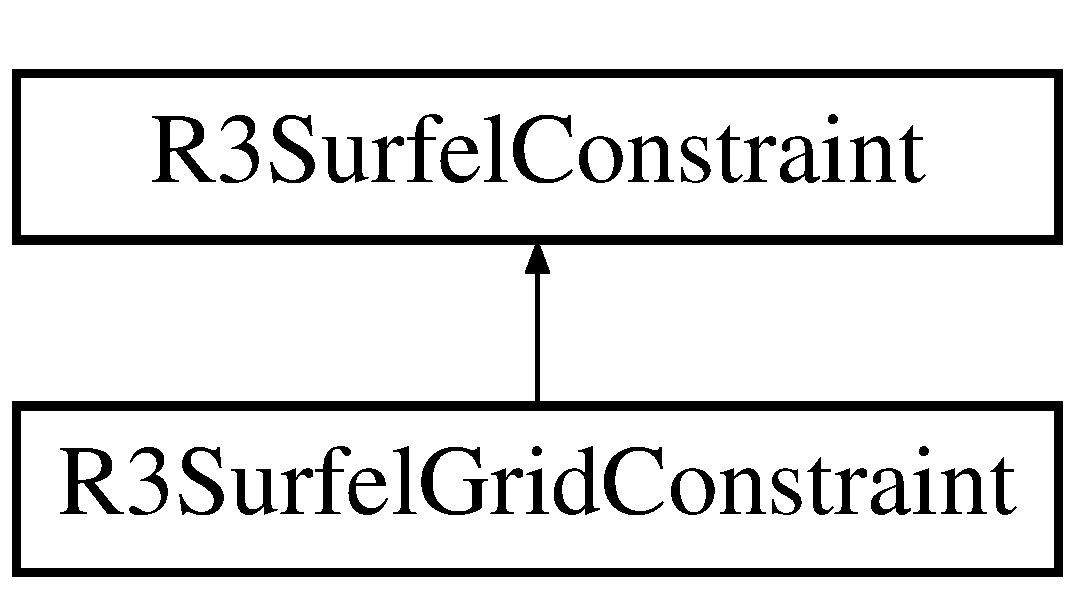
\includegraphics[height=2.000000cm]{class_r3_surfel_grid_constraint}
\end{center}
\end{figure}
\subsection*{Public Member Functions}
\begin{DoxyCompactItemize}
\item 
{\bfseries R3\+Surfel\+Grid\+Constraint} (const \hyperlink{class_r3_grid}{R3\+Grid} $\ast$grid, int comparison\+\_\+type=R3\+\_\+\+S\+U\+R\+F\+E\+L\+\_\+\+C\+O\+N\+S\+T\+R\+A\+I\+N\+T\+\_\+\+L\+E\+SS, int surfel\+\_\+value\+\_\+type=R3\+\_\+\+S\+U\+R\+F\+E\+L\+\_\+\+C\+O\+N\+S\+T\+R\+A\+I\+N\+T\+\_\+\+O\+P\+E\+R\+A\+ND, int grid\+\_\+value\+\_\+type=R3\+\_\+\+S\+U\+R\+F\+E\+L\+\_\+\+C\+O\+N\+S\+T\+R\+A\+I\+N\+T\+\_\+\+V\+A\+L\+UE, R\+N\+Scalar surfel\+\_\+operand=R\+N\+\_\+\+E\+P\+S\+I\+L\+ON, R\+N\+Scalar grid\+\_\+operand=0, R\+N\+Scalar epsilon=0)\hypertarget{class_r3_surfel_grid_constraint_a20c8e4506ed3020f6e2ab79a27e3c6e7}{}\label{class_r3_surfel_grid_constraint_a20c8e4506ed3020f6e2ab79a27e3c6e7}

\item 
virtual int {\bfseries Check} (const \hyperlink{class_r3_point}{R3\+Point} \&point) const \hypertarget{class_r3_surfel_grid_constraint_a4d7d00a332ca57b3ed3b0254f9950252}{}\label{class_r3_surfel_grid_constraint_a4d7d00a332ca57b3ed3b0254f9950252}

\item 
virtual int {\bfseries Check} (const \hyperlink{class_r3_box}{R3\+Box} \&\hyperlink{structbox}{box}) const \hypertarget{class_r3_surfel_grid_constraint_a6f42ae9412b08bd1d73265950fc64642}{}\label{class_r3_surfel_grid_constraint_a6f42ae9412b08bd1d73265950fc64642}

\end{DoxyCompactItemize}


The documentation for this class was generated from the following files\+:\begin{DoxyCompactItemize}
\item 
R3\+Surfels/R3\+Surfel\+Constraint.\+h\item 
R3\+Surfels/R3\+Surfel\+Constraint.\+cpp\end{DoxyCompactItemize}

\hypertarget{class_r3_surfel_halfspace_constraint}{}\section{R3\+Surfel\+Halfspace\+Constraint Class Reference}
\label{class_r3_surfel_halfspace_constraint}\index{R3\+Surfel\+Halfspace\+Constraint@{R3\+Surfel\+Halfspace\+Constraint}}
Inheritance diagram for R3\+Surfel\+Halfspace\+Constraint\+:\begin{figure}[H]
\begin{center}
\leavevmode
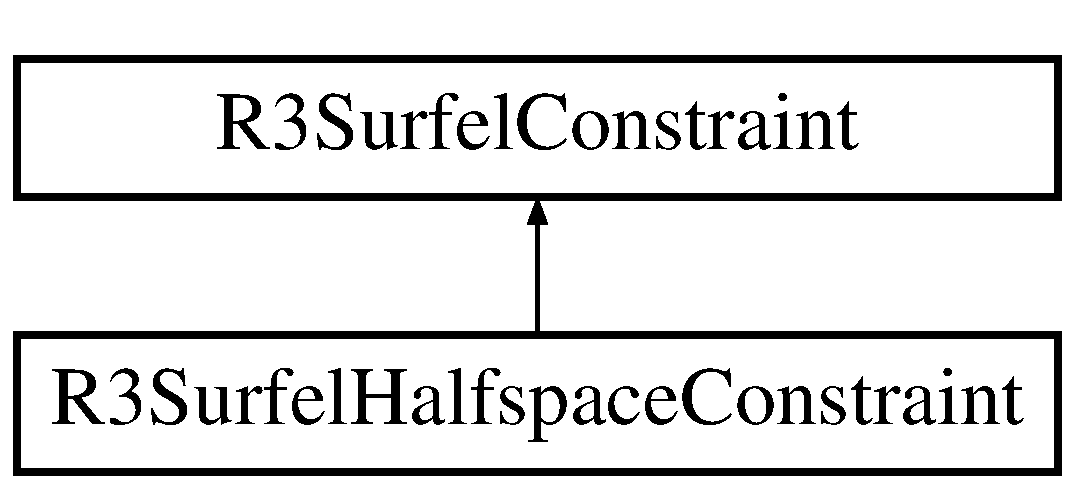
\includegraphics[height=2.000000cm]{class_r3_surfel_halfspace_constraint}
\end{center}
\end{figure}
\subsection*{Public Member Functions}
\begin{DoxyCompactItemize}
\item 
{\bfseries R3\+Surfel\+Halfspace\+Constraint} (const \hyperlink{class_r3_halfspace}{R3\+Halfspace} \&halfspace)\hypertarget{class_r3_surfel_halfspace_constraint_af550a5a58a2d38b2c42151eef4a11fce}{}\label{class_r3_surfel_halfspace_constraint_af550a5a58a2d38b2c42151eef4a11fce}

\item 
virtual int {\bfseries Check} (const \hyperlink{class_r3_point}{R3\+Point} \&point) const \hypertarget{class_r3_surfel_halfspace_constraint_a78ecbe1a999a62f30db878c6b186729c}{}\label{class_r3_surfel_halfspace_constraint_a78ecbe1a999a62f30db878c6b186729c}

\item 
virtual int {\bfseries Check} (const \hyperlink{class_r3_box}{R3\+Box} \&\hyperlink{structbox}{box}) const \hypertarget{class_r3_surfel_halfspace_constraint_ab22073db76565165649c2ea5ce1dae00}{}\label{class_r3_surfel_halfspace_constraint_ab22073db76565165649c2ea5ce1dae00}

\end{DoxyCompactItemize}


The documentation for this class was generated from the following files\+:\begin{DoxyCompactItemize}
\item 
R3\+Surfels/R3\+Surfel\+Constraint.\+h\item 
R3\+Surfels/R3\+Surfel\+Constraint.\+cpp\end{DoxyCompactItemize}

\hypertarget{class_r3_surfel_label}{}\section{R3\+Surfel\+Label Class Reference}
\label{class_r3_surfel_label}\index{R3\+Surfel\+Label@{R3\+Surfel\+Label}}
\subsection*{Public Member Functions}
\begin{DoxyCompactItemize}
\item 
{\bfseries R3\+Surfel\+Label} (const char $\ast$name=N\+U\+LL)\hypertarget{class_r3_surfel_label_aebc652da5780d9e2f8905806aa679221}{}\label{class_r3_surfel_label_aebc652da5780d9e2f8905806aa679221}

\item 
{\bfseries R3\+Surfel\+Label} (const \hyperlink{class_r3_surfel_label}{R3\+Surfel\+Label} \&label)\hypertarget{class_r3_surfel_label_a5b8fdefc5f5cb3f9ff0d6fe95a5f6dad}{}\label{class_r3_surfel_label_a5b8fdefc5f5cb3f9ff0d6fe95a5f6dad}

\item 
const char $\ast$ {\bfseries Name} (void) const \hypertarget{class_r3_surfel_label_a41d27293d048c6ed1ccb3f25c4ad7443}{}\label{class_r3_surfel_label_a41d27293d048c6ed1ccb3f25c4ad7443}

\item 
int {\bfseries Identifier} (void) const \hypertarget{class_r3_surfel_label_a70c808d2a3b6cca98edd34e5061ab202}{}\label{class_r3_surfel_label_a70c808d2a3b6cca98edd34e5061ab202}

\item 
int {\bfseries Assignment\+Keystroke} (void) const \hypertarget{class_r3_surfel_label_a780ab05994b400c61b1cd4346ce85c42}{}\label{class_r3_surfel_label_a780ab05994b400c61b1cd4346ce85c42}

\item 
const \hyperlink{class_r_n_rgb}{R\+N\+Rgb} \& {\bfseries Color} (void) const \hypertarget{class_r3_surfel_label_a3e6d13b2fe71252dd7af619cf9330a28}{}\label{class_r3_surfel_label_a3e6d13b2fe71252dd7af619cf9330a28}

\item 
void $\ast$ {\bfseries Data} (void) const \hypertarget{class_r3_surfel_label_ae1d641830fa025556ab0524c3703977d}{}\label{class_r3_surfel_label_ae1d641830fa025556ab0524c3703977d}

\item 
\hyperlink{class_r3_surfel_scene}{R3\+Surfel\+Scene} $\ast$ {\bfseries Scene} (void) const \hypertarget{class_r3_surfel_label_a4244977655cf59428481ad9dccee37dc}{}\label{class_r3_surfel_label_a4244977655cf59428481ad9dccee37dc}

\item 
int {\bfseries Scene\+Index} (void) const \hypertarget{class_r3_surfel_label_a8c429d2fa5dd108e5ac7b7e1047c5b38}{}\label{class_r3_surfel_label_a8c429d2fa5dd108e5ac7b7e1047c5b38}

\item 
int {\bfseries N\+Parts} (void) const \hypertarget{class_r3_surfel_label_a1fe4540dc64111f22a536dd66a988f5f}{}\label{class_r3_surfel_label_a1fe4540dc64111f22a536dd66a988f5f}

\item 
\hyperlink{class_r3_surfel_label}{R3\+Surfel\+Label} $\ast$ {\bfseries Part} (int k) const \hypertarget{class_r3_surfel_label_a50578dab1106fc14adfed338ddc93afe}{}\label{class_r3_surfel_label_a50578dab1106fc14adfed338ddc93afe}

\item 
\hyperlink{class_r3_surfel_label}{R3\+Surfel\+Label} $\ast$ {\bfseries Parent} (void) const \hypertarget{class_r3_surfel_label_aa3ef6a15d6e8cbcf4ff949633d8f4615}{}\label{class_r3_surfel_label_aa3ef6a15d6e8cbcf4ff949633d8f4615}

\item 
int {\bfseries Part\+Hierarchy\+Level} (void) const \hypertarget{class_r3_surfel_label_af93dee2555c8a35b535c1784b6b34600}{}\label{class_r3_surfel_label_af93dee2555c8a35b535c1784b6b34600}

\item 
int {\bfseries N\+Label\+Properties} (void) const \hypertarget{class_r3_surfel_label_a0fb3efa8ead0ac32768c9895dfe638c4}{}\label{class_r3_surfel_label_a0fb3efa8ead0ac32768c9895dfe638c4}

\item 
\hyperlink{class_r3_surfel_label_property}{R3\+Surfel\+Label\+Property} $\ast$ {\bfseries Label\+Property} (int k) const \hypertarget{class_r3_surfel_label_a4808bd997738b09c01fd151886ba9c5b}{}\label{class_r3_surfel_label_a4808bd997738b09c01fd151886ba9c5b}

\item 
\hyperlink{class_r3_surfel_label_property}{R3\+Surfel\+Label\+Property} $\ast$ {\bfseries Find\+Label\+Property} (int type) const \hypertarget{class_r3_surfel_label_a7f0fd40660afc803460bc529a2a24481}{}\label{class_r3_surfel_label_a7f0fd40660afc803460bc529a2a24481}

\item 
int {\bfseries N\+Label\+Relationships} (void) const \hypertarget{class_r3_surfel_label_a354f854deef51449e105e6fded508e48}{}\label{class_r3_surfel_label_a354f854deef51449e105e6fded508e48}

\item 
\hyperlink{class_r3_surfel_label_relationship}{R3\+Surfel\+Label\+Relationship} $\ast$ {\bfseries Label\+Relationship} (int k) const \hypertarget{class_r3_surfel_label_a9fdc750ebf65a76ff1690c95c86ee854}{}\label{class_r3_surfel_label_a9fdc750ebf65a76ff1690c95c86ee854}

\item 
int {\bfseries N\+Label\+Assignments} (void) const \hypertarget{class_r3_surfel_label_ab628648be5697fbd398906c2392fa351}{}\label{class_r3_surfel_label_ab628648be5697fbd398906c2392fa351}

\item 
\hyperlink{class_r3_surfel_label_assignment}{R3\+Surfel\+Label\+Assignment} $\ast$ {\bfseries Label\+Assignment} (int k) const \hypertarget{class_r3_surfel_label_adb06010dbc857b4ac598f1c66ebc0ab3}{}\label{class_r3_surfel_label_adb06010dbc857b4ac598f1c66ebc0ab3}

\item 
virtual void {\bfseries Set\+Parent} (\hyperlink{class_r3_surfel_label}{R3\+Surfel\+Label} $\ast$parent)\hypertarget{class_r3_surfel_label_a468bf63d36d6876e42656c5e2f25afd5}{}\label{class_r3_surfel_label_a468bf63d36d6876e42656c5e2f25afd5}

\item 
virtual void {\bfseries Set\+Name} (const char $\ast$name)\hypertarget{class_r3_surfel_label_aa6e27993469dd0bbd3959e257660161c}{}\label{class_r3_surfel_label_aa6e27993469dd0bbd3959e257660161c}

\item 
virtual void {\bfseries Set\+Identifier} (int identifier)\hypertarget{class_r3_surfel_label_a4b017c5e52b5e514f3e13da9b8b3c9ce}{}\label{class_r3_surfel_label_a4b017c5e52b5e514f3e13da9b8b3c9ce}

\item 
virtual void {\bfseries Set\+Assignment\+Keystroke} (int key)\hypertarget{class_r3_surfel_label_adcaeda32d5a251d9bcc7e49d86ec8de3}{}\label{class_r3_surfel_label_adcaeda32d5a251d9bcc7e49d86ec8de3}

\item 
virtual void {\bfseries Set\+Color} (const \hyperlink{class_r_n_rgb}{R\+N\+Rgb} \&color)\hypertarget{class_r3_surfel_label_a65dcdd715f6f6b30debf3a2759e27ced}{}\label{class_r3_surfel_label_a65dcdd715f6f6b30debf3a2759e27ced}

\item 
virtual void {\bfseries Set\+Data} (void $\ast$data)\hypertarget{class_r3_surfel_label_a36f112be5442f762177412fa0e2391ec}{}\label{class_r3_surfel_label_a36f112be5442f762177412fa0e2391ec}

\item 
virtual void {\bfseries Print} (F\+I\+LE $\ast$fp=N\+U\+LL, const char $\ast$prefix=N\+U\+LL, const char $\ast$suffix=N\+U\+LL) const \hypertarget{class_r3_surfel_label_a6cd67d905552acc8a45fa07855efa96e}{}\label{class_r3_surfel_label_a6cd67d905552acc8a45fa07855efa96e}

\end{DoxyCompactItemize}
\subsection*{Protected Member Functions}
\begin{DoxyCompactItemize}
\item 
void {\bfseries Update\+After\+Insert} (\hyperlink{class_r3_surfel_scene}{R3\+Surfel\+Scene} $\ast$scene)\hypertarget{class_r3_surfel_label_a0a0b408e12dfbab163b12f200676c013}{}\label{class_r3_surfel_label_a0a0b408e12dfbab163b12f200676c013}

\item 
void {\bfseries Update\+Before\+Remove} (\hyperlink{class_r3_surfel_scene}{R3\+Surfel\+Scene} $\ast$scene)\hypertarget{class_r3_surfel_label_a525e7a4ab723070f8900c4ecdf909e09}{}\label{class_r3_surfel_label_a525e7a4ab723070f8900c4ecdf909e09}

\item 
void {\bfseries Update\+After\+Insert\+Label\+Property} (\hyperlink{class_r3_surfel_label_property}{R3\+Surfel\+Label\+Property} $\ast$property)\hypertarget{class_r3_surfel_label_a091405d0a67c1195d7bb566f1f079e7e}{}\label{class_r3_surfel_label_a091405d0a67c1195d7bb566f1f079e7e}

\item 
void {\bfseries Update\+Before\+Remove\+Label\+Property} (\hyperlink{class_r3_surfel_label_property}{R3\+Surfel\+Label\+Property} $\ast$property)\hypertarget{class_r3_surfel_label_a4c0dd43aeb3aad46d4fdfaae314fa497}{}\label{class_r3_surfel_label_a4c0dd43aeb3aad46d4fdfaae314fa497}

\item 
void {\bfseries Update\+After\+Insert\+Label\+Relationship} (\hyperlink{class_r3_surfel_label_relationship}{R3\+Surfel\+Label\+Relationship} $\ast$relationship)\hypertarget{class_r3_surfel_label_a56c5cf7881603b3bd74393c2bacdf1e4}{}\label{class_r3_surfel_label_a56c5cf7881603b3bd74393c2bacdf1e4}

\item 
void {\bfseries Update\+Before\+Remove\+Label\+Relationship} (\hyperlink{class_r3_surfel_label_relationship}{R3\+Surfel\+Label\+Relationship} $\ast$relationship)\hypertarget{class_r3_surfel_label_ad9d11024abcae3f85eba724686adb9e2}{}\label{class_r3_surfel_label_ad9d11024abcae3f85eba724686adb9e2}

\item 
void {\bfseries Update\+After\+Insert\+Label\+Assignment} (\hyperlink{class_r3_surfel_label_assignment}{R3\+Surfel\+Label\+Assignment} $\ast$assignment)\hypertarget{class_r3_surfel_label_a1c2051536758514be2ca1cbfba01b931}{}\label{class_r3_surfel_label_a1c2051536758514be2ca1cbfba01b931}

\item 
void {\bfseries Update\+Before\+Remove\+Label\+Assignment} (\hyperlink{class_r3_surfel_label_assignment}{R3\+Surfel\+Label\+Assignment} $\ast$assignment)\hypertarget{class_r3_surfel_label_a795118e8cb76133660748a4fdcc37a33}{}\label{class_r3_surfel_label_a795118e8cb76133660748a4fdcc37a33}

\end{DoxyCompactItemize}
\subsection*{Protected Attributes}
\begin{DoxyCompactItemize}
\item 
\hyperlink{class_r3_surfel_scene}{R3\+Surfel\+Scene} $\ast$ {\bfseries scene}\hypertarget{class_r3_surfel_label_aba71a198a7111ba51045392fc6c2b2c6}{}\label{class_r3_surfel_label_aba71a198a7111ba51045392fc6c2b2c6}

\item 
int {\bfseries scene\+\_\+index}\hypertarget{class_r3_surfel_label_ab7996d8ac718c3ff24d8953ae6ab161a}{}\label{class_r3_surfel_label_ab7996d8ac718c3ff24d8953ae6ab161a}

\item 
\hyperlink{class_r3_surfel_label}{R3\+Surfel\+Label} $\ast$ {\bfseries parent}\hypertarget{class_r3_surfel_label_a0b88351cd1e669b6b083d081cdfeb4df}{}\label{class_r3_surfel_label_a0b88351cd1e669b6b083d081cdfeb4df}

\item 
\hyperlink{class_r_n_array}{R\+N\+Array}$<$ \hyperlink{class_r3_surfel_label}{R3\+Surfel\+Label} $\ast$ $>$ {\bfseries parts}\hypertarget{class_r3_surfel_label_ad1789b91b0893bb7b812d3bf88647ae7}{}\label{class_r3_surfel_label_ad1789b91b0893bb7b812d3bf88647ae7}

\item 
\hyperlink{class_r_n_array}{R\+N\+Array}$<$ \hyperlink{class_r3_surfel_label_property}{R3\+Surfel\+Label\+Property} $\ast$ $>$ {\bfseries properties}\hypertarget{class_r3_surfel_label_a141ad437d5a29560d99499ef8916a9fb}{}\label{class_r3_surfel_label_a141ad437d5a29560d99499ef8916a9fb}

\item 
\hyperlink{class_r_n_array}{R\+N\+Array}$<$ \hyperlink{class_r3_surfel_label_relationship}{R3\+Surfel\+Label\+Relationship} $\ast$ $>$ {\bfseries relationships}\hypertarget{class_r3_surfel_label_acaddd66872c39453285ec5d4a98ba60c}{}\label{class_r3_surfel_label_acaddd66872c39453285ec5d4a98ba60c}

\item 
\hyperlink{class_r_n_array}{R\+N\+Array}$<$ \hyperlink{class_r3_surfel_label_assignment}{R3\+Surfel\+Label\+Assignment} $\ast$ $>$ {\bfseries assignments}\hypertarget{class_r3_surfel_label_ac2259cace360e553e4d6a97b58251db2}{}\label{class_r3_surfel_label_ac2259cace360e553e4d6a97b58251db2}

\item 
char $\ast$ {\bfseries name}\hypertarget{class_r3_surfel_label_a0b5cb42f53160a1dad6f9866ed7b83e4}{}\label{class_r3_surfel_label_a0b5cb42f53160a1dad6f9866ed7b83e4}

\item 
int {\bfseries identifier}\hypertarget{class_r3_surfel_label_a1d91e8e830f8d2bc3e6b6608dc035122}{}\label{class_r3_surfel_label_a1d91e8e830f8d2bc3e6b6608dc035122}

\item 
int {\bfseries assignment\+\_\+keystroke}\hypertarget{class_r3_surfel_label_aed8f801a39dece745044f14008b60603}{}\label{class_r3_surfel_label_aed8f801a39dece745044f14008b60603}

\item 
\hyperlink{class_r_n_rgb}{R\+N\+Rgb} {\bfseries color}\hypertarget{class_r3_surfel_label_ac314cb5865128c9dbe6d4ab72afe343f}{}\label{class_r3_surfel_label_ac314cb5865128c9dbe6d4ab72afe343f}

\item 
void $\ast$ {\bfseries data}\hypertarget{class_r3_surfel_label_a1ed9c4b4e317412446cfd45d69213ca5}{}\label{class_r3_surfel_label_a1ed9c4b4e317412446cfd45d69213ca5}

\end{DoxyCompactItemize}
\subsection*{Friends}
\begin{DoxyCompactItemize}
\item 
class {\bfseries R3\+Surfel\+Scene}\hypertarget{class_r3_surfel_label_af9bb32c0eac7d1d54787bbc6b44586b6}{}\label{class_r3_surfel_label_af9bb32c0eac7d1d54787bbc6b44586b6}

\end{DoxyCompactItemize}


The documentation for this class was generated from the following files\+:\begin{DoxyCompactItemize}
\item 
R3\+Surfels/R3\+Surfel\+Label.\+h\item 
R3\+Surfels/R3\+Surfel\+Label.\+cpp\end{DoxyCompactItemize}

\hypertarget{class_r3_surfel_label_assignment}{}\section{R3\+Surfel\+Label\+Assignment Class Reference}
\label{class_r3_surfel_label_assignment}\index{R3\+Surfel\+Label\+Assignment@{R3\+Surfel\+Label\+Assignment}}
\subsection*{Public Member Functions}
\begin{DoxyCompactItemize}
\item 
{\bfseries R3\+Surfel\+Label\+Assignment} (\hyperlink{class_r3_surfel_object}{R3\+Surfel\+Object} $\ast$object=N\+U\+LL, \hyperlink{class_r3_surfel_label}{R3\+Surfel\+Label} $\ast$label=N\+U\+LL, double confidence=0, int originator=0)\hypertarget{class_r3_surfel_label_assignment_a9466bcb95619bb23c8359a7bb36723f4}{}\label{class_r3_surfel_label_assignment_a9466bcb95619bb23c8359a7bb36723f4}

\item 
{\bfseries R3\+Surfel\+Label\+Assignment} (const \hyperlink{class_r3_surfel_label_assignment}{R3\+Surfel\+Label\+Assignment} \&assignment)\hypertarget{class_r3_surfel_label_assignment_a8a91dee55101fc0b9d15eab6dbd572f6}{}\label{class_r3_surfel_label_assignment_a8a91dee55101fc0b9d15eab6dbd572f6}

\item 
double {\bfseries Confidence} (void) const \hypertarget{class_r3_surfel_label_assignment_a4dcbabb8300a6ff9c06d87e4389294e6}{}\label{class_r3_surfel_label_assignment_a4dcbabb8300a6ff9c06d87e4389294e6}

\item 
int {\bfseries Originator} (void) const \hypertarget{class_r3_surfel_label_assignment_a29c28d04e6b45991e543d4dd9fff42bf}{}\label{class_r3_surfel_label_assignment_a29c28d04e6b45991e543d4dd9fff42bf}

\item 
void $\ast$ {\bfseries Data} (void) const \hypertarget{class_r3_surfel_label_assignment_a227ab6712b63c6ae7993c8eb22a05814}{}\label{class_r3_surfel_label_assignment_a227ab6712b63c6ae7993c8eb22a05814}

\item 
\hyperlink{class_r3_surfel_scene}{R3\+Surfel\+Scene} $\ast$ {\bfseries Scene} (void) const \hypertarget{class_r3_surfel_label_assignment_a7c6434171ae949babaaa5f5b15c16724}{}\label{class_r3_surfel_label_assignment_a7c6434171ae949babaaa5f5b15c16724}

\item 
int {\bfseries Scene\+Index} (void) const \hypertarget{class_r3_surfel_label_assignment_a111c6971f060d4c677a9056e99bdd641}{}\label{class_r3_surfel_label_assignment_a111c6971f060d4c677a9056e99bdd641}

\item 
\hyperlink{class_r3_surfel_object}{R3\+Surfel\+Object} $\ast$ {\bfseries Object} (void) const \hypertarget{class_r3_surfel_label_assignment_aba4bc7ffdf2032c95765639eb50517a7}{}\label{class_r3_surfel_label_assignment_aba4bc7ffdf2032c95765639eb50517a7}

\item 
int {\bfseries Object\+Index} (void) const \hypertarget{class_r3_surfel_label_assignment_a1d018ce5951f22b98b8c7a2ca69e51ca}{}\label{class_r3_surfel_label_assignment_a1d018ce5951f22b98b8c7a2ca69e51ca}

\item 
\hyperlink{class_r3_surfel_label}{R3\+Surfel\+Label} $\ast$ {\bfseries Label} (void) const \hypertarget{class_r3_surfel_label_assignment_a3c58553bc95aff6418a175e051b5ff79}{}\label{class_r3_surfel_label_assignment_a3c58553bc95aff6418a175e051b5ff79}

\item 
int {\bfseries Label\+Index} (void) const \hypertarget{class_r3_surfel_label_assignment_a47223c3eb9836c56cadd63954d505595}{}\label{class_r3_surfel_label_assignment_a47223c3eb9836c56cadd63954d505595}

\item 
void {\bfseries Set\+Confidence} (double confidence)\hypertarget{class_r3_surfel_label_assignment_a30327c9851c9bfdf9afda5ce8177bc81}{}\label{class_r3_surfel_label_assignment_a30327c9851c9bfdf9afda5ce8177bc81}

\item 
void {\bfseries Set\+Originator} (int originator)\hypertarget{class_r3_surfel_label_assignment_a44787a9c4e8a0a7131a59afcf544ab02}{}\label{class_r3_surfel_label_assignment_a44787a9c4e8a0a7131a59afcf544ab02}

\item 
virtual void {\bfseries Set\+Data} (void $\ast$data)\hypertarget{class_r3_surfel_label_assignment_a92d9be123ed16edd59eeadf40e990bd6}{}\label{class_r3_surfel_label_assignment_a92d9be123ed16edd59eeadf40e990bd6}

\end{DoxyCompactItemize}
\subsection*{Protected Member Functions}
\begin{DoxyCompactItemize}
\item 
void {\bfseries Update\+After\+Insert} (\hyperlink{class_r3_surfel_scene}{R3\+Surfel\+Scene} $\ast$scene)\hypertarget{class_r3_surfel_label_assignment_aa99120b98cba0f5a8653cefe63c23bc6}{}\label{class_r3_surfel_label_assignment_aa99120b98cba0f5a8653cefe63c23bc6}

\item 
void {\bfseries Update\+Before\+Remove} (\hyperlink{class_r3_surfel_scene}{R3\+Surfel\+Scene} $\ast$scene)\hypertarget{class_r3_surfel_label_assignment_a946a3e605e9d8b9ed4d80406f02178fa}{}\label{class_r3_surfel_label_assignment_a946a3e605e9d8b9ed4d80406f02178fa}

\end{DoxyCompactItemize}
\subsection*{Protected Attributes}
\begin{DoxyCompactItemize}
\item 
\hyperlink{class_r3_surfel_scene}{R3\+Surfel\+Scene} $\ast$ {\bfseries scene}\hypertarget{class_r3_surfel_label_assignment_afcf0458e726dab9a68a11f29e471dad2}{}\label{class_r3_surfel_label_assignment_afcf0458e726dab9a68a11f29e471dad2}

\item 
int {\bfseries scene\+\_\+index}\hypertarget{class_r3_surfel_label_assignment_a29e442232ea367ecd80ceb8cfbe901f5}{}\label{class_r3_surfel_label_assignment_a29e442232ea367ecd80ceb8cfbe901f5}

\item 
\hyperlink{class_r3_surfel_object}{R3\+Surfel\+Object} $\ast$ {\bfseries object}\hypertarget{class_r3_surfel_label_assignment_ac77b43fa6c303ebb35f0b402412d872c}{}\label{class_r3_surfel_label_assignment_ac77b43fa6c303ebb35f0b402412d872c}

\item 
int {\bfseries object\+\_\+index}\hypertarget{class_r3_surfel_label_assignment_a34bf573676f5bef511128911596a3bf7}{}\label{class_r3_surfel_label_assignment_a34bf573676f5bef511128911596a3bf7}

\item 
\hyperlink{class_r3_surfel_label}{R3\+Surfel\+Label} $\ast$ {\bfseries label}\hypertarget{class_r3_surfel_label_assignment_a583ace2dfe0a2e05b7dcc7a2d6737221}{}\label{class_r3_surfel_label_assignment_a583ace2dfe0a2e05b7dcc7a2d6737221}

\item 
int {\bfseries label\+\_\+index}\hypertarget{class_r3_surfel_label_assignment_ac4a7f6d987643fc60b6ccfde5f89aab2}{}\label{class_r3_surfel_label_assignment_ac4a7f6d987643fc60b6ccfde5f89aab2}

\item 
double {\bfseries confidence}\hypertarget{class_r3_surfel_label_assignment_ae68249f02cb78c04cbbba02727686f28}{}\label{class_r3_surfel_label_assignment_ae68249f02cb78c04cbbba02727686f28}

\item 
int {\bfseries originator}\hypertarget{class_r3_surfel_label_assignment_a80ab6de24598c308f761ea8591f81627}{}\label{class_r3_surfel_label_assignment_a80ab6de24598c308f761ea8591f81627}

\item 
void $\ast$ {\bfseries data}\hypertarget{class_r3_surfel_label_assignment_a18d2b431365505d2e271cd5dce29b786}{}\label{class_r3_surfel_label_assignment_a18d2b431365505d2e271cd5dce29b786}

\end{DoxyCompactItemize}
\subsection*{Friends}
\begin{DoxyCompactItemize}
\item 
class {\bfseries R3\+Surfel\+Scene}\hypertarget{class_r3_surfel_label_assignment_af9bb32c0eac7d1d54787bbc6b44586b6}{}\label{class_r3_surfel_label_assignment_af9bb32c0eac7d1d54787bbc6b44586b6}

\item 
class {\bfseries R3\+Surfel\+Object}\hypertarget{class_r3_surfel_label_assignment_a850b1452c6e8af94bc02cc26bd2e5fe8}{}\label{class_r3_surfel_label_assignment_a850b1452c6e8af94bc02cc26bd2e5fe8}

\item 
class {\bfseries R3\+Surfel\+Label}\hypertarget{class_r3_surfel_label_assignment_a5f8429227744e4e08e5a44a3fcba527f}{}\label{class_r3_surfel_label_assignment_a5f8429227744e4e08e5a44a3fcba527f}

\end{DoxyCompactItemize}


The documentation for this class was generated from the following files\+:\begin{DoxyCompactItemize}
\item 
R3\+Surfels/R3\+Surfel\+Label\+Assignment.\+h\item 
R3\+Surfels/R3\+Surfel\+Label\+Assignment.\+cpp\end{DoxyCompactItemize}

\hypertarget{class_r3_surfel_label_constraint}{}\section{R3\+Surfel\+Label\+Constraint Class Reference}
\label{class_r3_surfel_label_constraint}\index{R3\+Surfel\+Label\+Constraint@{R3\+Surfel\+Label\+Constraint}}
Inheritance diagram for R3\+Surfel\+Label\+Constraint\+:\begin{figure}[H]
\begin{center}
\leavevmode
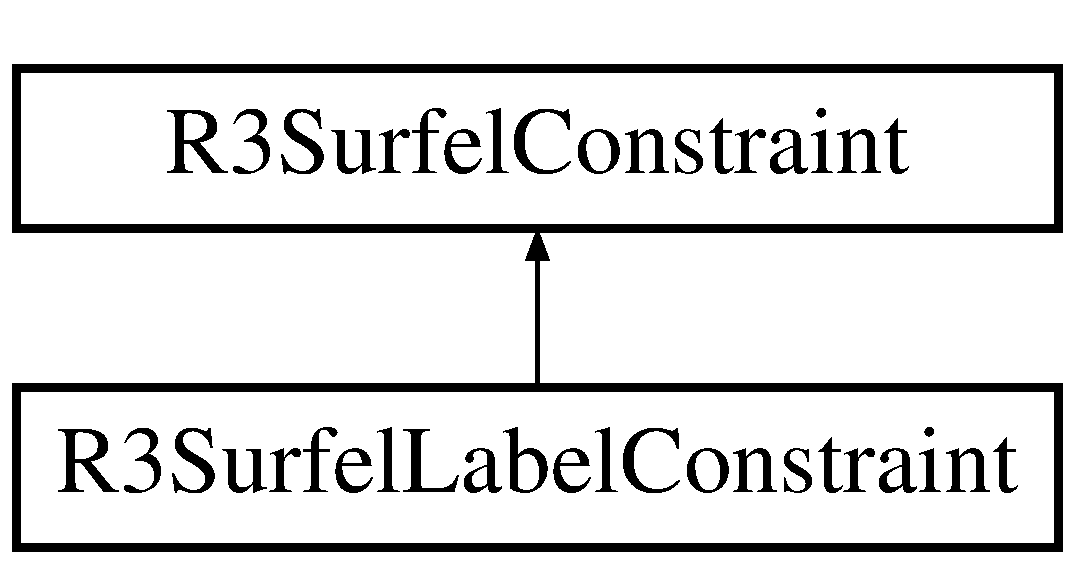
\includegraphics[height=2.000000cm]{class_r3_surfel_label_constraint}
\end{center}
\end{figure}
\subsection*{Public Member Functions}
\begin{DoxyCompactItemize}
\item 
{\bfseries R3\+Surfel\+Label\+Constraint} (\hyperlink{class_r3_surfel_label}{R3\+Surfel\+Label} $\ast$target\+\_\+label=N\+U\+LL, R\+N\+Boolean converse=F\+A\+L\+SE)\hypertarget{class_r3_surfel_label_constraint_a9a53701580bee43b2bafea95004e2803}{}\label{class_r3_surfel_label_constraint_a9a53701580bee43b2bafea95004e2803}

\item 
virtual int {\bfseries Check} (const \hyperlink{class_r3_surfel_object}{R3\+Surfel\+Object} $\ast$object) const \hypertarget{class_r3_surfel_label_constraint_a203831fe20513e99a9485f9347200ff3}{}\label{class_r3_surfel_label_constraint_a203831fe20513e99a9485f9347200ff3}

\item 
virtual int {\bfseries Check} (const \hyperlink{class_r3_surfel_node}{R3\+Surfel\+Node} $\ast$node) const \hypertarget{class_r3_surfel_label_constraint_a888a2876808c2a36710373205c0c3ee3}{}\label{class_r3_surfel_label_constraint_a888a2876808c2a36710373205c0c3ee3}

\item 
virtual int {\bfseries Check} (const \hyperlink{class_r3_surfel_block}{R3\+Surfel\+Block} $\ast$block) const \hypertarget{class_r3_surfel_label_constraint_acc5535d71d57631b2637e9389fe7c56a}{}\label{class_r3_surfel_label_constraint_acc5535d71d57631b2637e9389fe7c56a}

\item 
virtual int {\bfseries Check} (const \hyperlink{class_r3_surfel_block}{R3\+Surfel\+Block} $\ast$block, const \hyperlink{class_r3_surfel}{R3\+Surfel} $\ast$surfel) const \hypertarget{class_r3_surfel_label_constraint_ab88001637c1d280367f16ddff82c4fe6}{}\label{class_r3_surfel_label_constraint_ab88001637c1d280367f16ddff82c4fe6}

\end{DoxyCompactItemize}


The documentation for this class was generated from the following files\+:\begin{DoxyCompactItemize}
\item 
R3\+Surfels/R3\+Surfel\+Constraint.\+h\item 
R3\+Surfels/R3\+Surfel\+Constraint.\+cpp\end{DoxyCompactItemize}

\hypertarget{class_r3_surfel_label_property}{}\section{R3\+Surfel\+Label\+Property Class Reference}
\label{class_r3_surfel_label_property}\index{R3\+Surfel\+Label\+Property@{R3\+Surfel\+Label\+Property}}
\subsection*{Public Member Functions}
\begin{DoxyCompactItemize}
\item 
{\bfseries R3\+Surfel\+Label\+Property} (int type=0, \hyperlink{class_r3_surfel_label}{R3\+Surfel\+Label} $\ast$label=N\+U\+LL, R\+N\+Scalar $\ast$operands=N\+U\+LL, int noperands=0)\hypertarget{class_r3_surfel_label_property_a686f20345d54be06a916b05f14f4586c}{}\label{class_r3_surfel_label_property_a686f20345d54be06a916b05f14f4586c}

\item 
{\bfseries R3\+Surfel\+Label\+Property} (const \hyperlink{class_r3_surfel_label_property}{R3\+Surfel\+Label\+Property} \&property)\hypertarget{class_r3_surfel_label_property_abc90d633ddd410fbdcc8ffcfe7774fdd}{}\label{class_r3_surfel_label_property_abc90d633ddd410fbdcc8ffcfe7774fdd}

\item 
int {\bfseries Type} (void) const \hypertarget{class_r3_surfel_label_property_a117d2cd83e7c1e54b38443adf257d509}{}\label{class_r3_surfel_label_property_a117d2cd83e7c1e54b38443adf257d509}

\item 
\hyperlink{class_r3_surfel_scene}{R3\+Surfel\+Scene} $\ast$ {\bfseries Scene} (void) const \hypertarget{class_r3_surfel_label_property_a9a99f21e18ee9c064dfd0f2a224f081a}{}\label{class_r3_surfel_label_property_a9a99f21e18ee9c064dfd0f2a224f081a}

\item 
int {\bfseries Scene\+Index} (void) const \hypertarget{class_r3_surfel_label_property_a52c4c1f762f8b6aab886d5fad9add2f5}{}\label{class_r3_surfel_label_property_a52c4c1f762f8b6aab886d5fad9add2f5}

\item 
\hyperlink{class_r3_surfel_label}{R3\+Surfel\+Label} $\ast$ {\bfseries Label} (void) const \hypertarget{class_r3_surfel_label_property_acbb6cf829bdc3ba8185223deeb0380b3}{}\label{class_r3_surfel_label_property_acbb6cf829bdc3ba8185223deeb0380b3}

\item 
int {\bfseries N\+Operands} (void) const \hypertarget{class_r3_surfel_label_property_afe49ee3643a307edac3c1d56b5e30c5f}{}\label{class_r3_surfel_label_property_afe49ee3643a307edac3c1d56b5e30c5f}

\item 
R\+N\+Scalar {\bfseries Operand} (int k) const \hypertarget{class_r3_surfel_label_property_adf7fd3c411daed82c9d40792575fea74}{}\label{class_r3_surfel_label_property_adf7fd3c411daed82c9d40792575fea74}

\end{DoxyCompactItemize}
\subsection*{Static Public Member Functions}
\begin{DoxyCompactItemize}
\item 
static int {\bfseries N\+Operands} (int type)\hypertarget{class_r3_surfel_label_property_ac0cadace07095226d611f80863c0a361}{}\label{class_r3_surfel_label_property_ac0cadace07095226d611f80863c0a361}

\end{DoxyCompactItemize}
\subsection*{Protected Member Functions}
\begin{DoxyCompactItemize}
\item 
void {\bfseries Update\+After\+Insert} (\hyperlink{class_r3_surfel_scene}{R3\+Surfel\+Scene} $\ast$scene)\hypertarget{class_r3_surfel_label_property_a7fa11c2eddf30a8f04e27096df0bc426}{}\label{class_r3_surfel_label_property_a7fa11c2eddf30a8f04e27096df0bc426}

\item 
void {\bfseries Update\+Before\+Remove} (\hyperlink{class_r3_surfel_scene}{R3\+Surfel\+Scene} $\ast$scene)\hypertarget{class_r3_surfel_label_property_ab39be68c10a1883c3db023135d696836}{}\label{class_r3_surfel_label_property_ab39be68c10a1883c3db023135d696836}

\end{DoxyCompactItemize}
\subsection*{Protected Attributes}
\begin{DoxyCompactItemize}
\item 
\hyperlink{class_r3_surfel_scene}{R3\+Surfel\+Scene} $\ast$ {\bfseries scene}\hypertarget{class_r3_surfel_label_property_a0d72a1711885091e63f52529ead36d8a}{}\label{class_r3_surfel_label_property_a0d72a1711885091e63f52529ead36d8a}

\item 
int {\bfseries scene\+\_\+index}\hypertarget{class_r3_surfel_label_property_adca517e6d5281f9dfbce896b2baf2adc}{}\label{class_r3_surfel_label_property_adca517e6d5281f9dfbce896b2baf2adc}

\item 
\hyperlink{class_r3_surfel_label}{R3\+Surfel\+Label} $\ast$ {\bfseries label}\hypertarget{class_r3_surfel_label_property_a06ea65e4c2dd847be2dbd307b5134c5c}{}\label{class_r3_surfel_label_property_a06ea65e4c2dd847be2dbd307b5134c5c}

\item 
R\+N\+Scalar $\ast$ {\bfseries operands}\hypertarget{class_r3_surfel_label_property_aa34b1affdf56b7061d8bcab2b40926f8}{}\label{class_r3_surfel_label_property_aa34b1affdf56b7061d8bcab2b40926f8}

\item 
int {\bfseries noperands}\hypertarget{class_r3_surfel_label_property_a0cc06793af4a19672b6b7dc3c08610d4}{}\label{class_r3_surfel_label_property_a0cc06793af4a19672b6b7dc3c08610d4}

\item 
int {\bfseries type}\hypertarget{class_r3_surfel_label_property_ab9c08661479fafee2cb063cd937670dc}{}\label{class_r3_surfel_label_property_ab9c08661479fafee2cb063cd937670dc}

\end{DoxyCompactItemize}
\subsection*{Friends}
\begin{DoxyCompactItemize}
\item 
class {\bfseries R3\+Surfel\+Scene}\hypertarget{class_r3_surfel_label_property_af9bb32c0eac7d1d54787bbc6b44586b6}{}\label{class_r3_surfel_label_property_af9bb32c0eac7d1d54787bbc6b44586b6}

\end{DoxyCompactItemize}


The documentation for this class was generated from the following files\+:\begin{DoxyCompactItemize}
\item 
R3\+Surfels/R3\+Surfel\+Label\+Property.\+h\item 
R3\+Surfels/R3\+Surfel\+Label\+Property.\+cpp\end{DoxyCompactItemize}

\hypertarget{class_r3_surfel_label_relationship}{}\section{R3\+Surfel\+Label\+Relationship Class Reference}
\label{class_r3_surfel_label_relationship}\index{R3\+Surfel\+Label\+Relationship@{R3\+Surfel\+Label\+Relationship}}
\subsection*{Public Member Functions}
\begin{DoxyCompactItemize}
\item 
{\bfseries R3\+Surfel\+Label\+Relationship} (int type=0, \hyperlink{class_r3_surfel_label}{R3\+Surfel\+Label} $\ast$label0=N\+U\+LL, \hyperlink{class_r3_surfel_label}{R3\+Surfel\+Label} $\ast$label1=N\+U\+LL, R\+N\+Scalar $\ast$operands=N\+U\+LL, int noperands=0)\hypertarget{class_r3_surfel_label_relationship_a6923d902057d3ef9d19a521435aa8bfc}{}\label{class_r3_surfel_label_relationship_a6923d902057d3ef9d19a521435aa8bfc}

\item 
{\bfseries R3\+Surfel\+Label\+Relationship} (int type, const \hyperlink{class_r_n_array}{R\+N\+Array}$<$ \hyperlink{class_r3_surfel_label}{R3\+Surfel\+Label} $\ast$ $>$ \&labels, R\+N\+Scalar $\ast$operands=N\+U\+LL, int noperands=0)\hypertarget{class_r3_surfel_label_relationship_ab066ff8d9a3ba4429d7cbb70747325db}{}\label{class_r3_surfel_label_relationship_ab066ff8d9a3ba4429d7cbb70747325db}

\item 
{\bfseries R3\+Surfel\+Label\+Relationship} (const \hyperlink{class_r3_surfel_label_relationship}{R3\+Surfel\+Label\+Relationship} \&relationship)\hypertarget{class_r3_surfel_label_relationship_ac9ce4496a49c3ced8d3b118d449d7ca7}{}\label{class_r3_surfel_label_relationship_ac9ce4496a49c3ced8d3b118d449d7ca7}

\item 
int {\bfseries Type} (void) const \hypertarget{class_r3_surfel_label_relationship_a0d058eda773d14cd611ed22105590a7f}{}\label{class_r3_surfel_label_relationship_a0d058eda773d14cd611ed22105590a7f}

\item 
\hyperlink{class_r3_surfel_scene}{R3\+Surfel\+Scene} $\ast$ {\bfseries Scene} (void) const \hypertarget{class_r3_surfel_label_relationship_a064d12e58b752dd8b096ca9cfc24ce77}{}\label{class_r3_surfel_label_relationship_a064d12e58b752dd8b096ca9cfc24ce77}

\item 
int {\bfseries Scene\+Index} (void) const \hypertarget{class_r3_surfel_label_relationship_a4f364225f4571b94dd6704c3f10a4873}{}\label{class_r3_surfel_label_relationship_a4f364225f4571b94dd6704c3f10a4873}

\item 
int {\bfseries N\+Labels} (void) const \hypertarget{class_r3_surfel_label_relationship_ad346230de5c825588dde5a0f00fe011c}{}\label{class_r3_surfel_label_relationship_ad346230de5c825588dde5a0f00fe011c}

\item 
\hyperlink{class_r3_surfel_label}{R3\+Surfel\+Label} $\ast$ {\bfseries Label} (int k) const \hypertarget{class_r3_surfel_label_relationship_a2bca8cacb9ade015223bbd093f176ef9}{}\label{class_r3_surfel_label_relationship_a2bca8cacb9ade015223bbd093f176ef9}

\item 
int {\bfseries N\+Operands} (void) const \hypertarget{class_r3_surfel_label_relationship_a57dc73ea095f5640391094385b6e50c4}{}\label{class_r3_surfel_label_relationship_a57dc73ea095f5640391094385b6e50c4}

\item 
R\+N\+Scalar {\bfseries Operand} (int k) const \hypertarget{class_r3_surfel_label_relationship_aa61dbfd72580234597e21e05edb19484}{}\label{class_r3_surfel_label_relationship_aa61dbfd72580234597e21e05edb19484}

\end{DoxyCompactItemize}
\subsection*{Protected Member Functions}
\begin{DoxyCompactItemize}
\item 
void {\bfseries Update\+After\+Insert} (\hyperlink{class_r3_surfel_scene}{R3\+Surfel\+Scene} $\ast$scene)\hypertarget{class_r3_surfel_label_relationship_a776ecc9c7f71c710c723cb163747bcb8}{}\label{class_r3_surfel_label_relationship_a776ecc9c7f71c710c723cb163747bcb8}

\item 
void {\bfseries Update\+Before\+Remove} (\hyperlink{class_r3_surfel_scene}{R3\+Surfel\+Scene} $\ast$scene)\hypertarget{class_r3_surfel_label_relationship_a0568cde8b34b5268ecaa6c07f9d05280}{}\label{class_r3_surfel_label_relationship_a0568cde8b34b5268ecaa6c07f9d05280}

\end{DoxyCompactItemize}
\subsection*{Protected Attributes}
\begin{DoxyCompactItemize}
\item 
\hyperlink{class_r3_surfel_scene}{R3\+Surfel\+Scene} $\ast$ {\bfseries scene}\hypertarget{class_r3_surfel_label_relationship_a37162c1d65f359c56d635746480c0a88}{}\label{class_r3_surfel_label_relationship_a37162c1d65f359c56d635746480c0a88}

\item 
int {\bfseries scene\+\_\+index}\hypertarget{class_r3_surfel_label_relationship_a90cd20a53bfe23faf32b1ef5765c8cf4}{}\label{class_r3_surfel_label_relationship_a90cd20a53bfe23faf32b1ef5765c8cf4}

\item 
\hyperlink{class_r_n_array}{R\+N\+Array}$<$ \hyperlink{class_r3_surfel_label}{R3\+Surfel\+Label} $\ast$ $>$ {\bfseries labels}\hypertarget{class_r3_surfel_label_relationship_a4106c48cc0af8bebda19e7deea3d9cb0}{}\label{class_r3_surfel_label_relationship_a4106c48cc0af8bebda19e7deea3d9cb0}

\item 
R\+N\+Scalar $\ast$ {\bfseries operands}\hypertarget{class_r3_surfel_label_relationship_a11cab2631979a169053125d646a1945f}{}\label{class_r3_surfel_label_relationship_a11cab2631979a169053125d646a1945f}

\item 
int {\bfseries noperands}\hypertarget{class_r3_surfel_label_relationship_af792472e0e6b63d0e16698d4c45bed48}{}\label{class_r3_surfel_label_relationship_af792472e0e6b63d0e16698d4c45bed48}

\item 
int {\bfseries type}\hypertarget{class_r3_surfel_label_relationship_a9300116969a70b5e7255ff5855911fc3}{}\label{class_r3_surfel_label_relationship_a9300116969a70b5e7255ff5855911fc3}

\end{DoxyCompactItemize}
\subsection*{Friends}
\begin{DoxyCompactItemize}
\item 
class {\bfseries R3\+Surfel\+Scene}\hypertarget{class_r3_surfel_label_relationship_af9bb32c0eac7d1d54787bbc6b44586b6}{}\label{class_r3_surfel_label_relationship_af9bb32c0eac7d1d54787bbc6b44586b6}

\end{DoxyCompactItemize}


The documentation for this class was generated from the following files\+:\begin{DoxyCompactItemize}
\item 
R3\+Surfels/R3\+Surfel\+Label\+Relationship.\+h\item 
R3\+Surfels/R3\+Surfel\+Label\+Relationship.\+cpp\end{DoxyCompactItemize}

\hypertarget{class_r3_surfel_label_set}{}\section{R3\+Surfel\+Label\+Set Class Reference}
\label{class_r3_surfel_label_set}\index{R3\+Surfel\+Label\+Set@{R3\+Surfel\+Label\+Set}}
\subsection*{Public Member Functions}
\begin{DoxyCompactItemize}
\item 
{\bfseries R3\+Surfel\+Label\+Set} (const \hyperlink{class_r3_surfel_label_set}{R3\+Surfel\+Label\+Set} \&set)\hypertarget{class_r3_surfel_label_set_a031bca208c2bb6d66b327e5549b47369}{}\label{class_r3_surfel_label_set_a031bca208c2bb6d66b327e5549b47369}

\item 
int {\bfseries N\+Labels} (void) const \hypertarget{class_r3_surfel_label_set_ad144d7997a9c50cb2d07aa804877328a}{}\label{class_r3_surfel_label_set_ad144d7997a9c50cb2d07aa804877328a}

\item 
\hyperlink{class_r3_surfel_label}{R3\+Surfel\+Label} $\ast$ {\bfseries Label} (int k) const \hypertarget{class_r3_surfel_label_set_aeddef05650b16ed5188bf16d5f9ca4b7}{}\label{class_r3_surfel_label_set_aeddef05650b16ed5188bf16d5f9ca4b7}

\item 
\hyperlink{class_r3_surfel_label}{R3\+Surfel\+Label} $\ast$ {\bfseries operator\mbox{[}$\,$\mbox{]}} (int k) const \hypertarget{class_r3_surfel_label_set_a34268796991f7f6be097aa49fbb79057}{}\label{class_r3_surfel_label_set_a34268796991f7f6be097aa49fbb79057}

\item 
virtual void {\bfseries Insert\+Label} (\hyperlink{class_r3_surfel_label}{R3\+Surfel\+Label} $\ast$label)\hypertarget{class_r3_surfel_label_set_a80e1e8306e033da9f12072de07e9ad44}{}\label{class_r3_surfel_label_set_a80e1e8306e033da9f12072de07e9ad44}

\item 
virtual void {\bfseries Remove\+Label} (\hyperlink{class_r3_surfel_label}{R3\+Surfel\+Label} $\ast$label)\hypertarget{class_r3_surfel_label_set_a31821c5446c048f566d93fb1ae9beeed}{}\label{class_r3_surfel_label_set_a31821c5446c048f566d93fb1ae9beeed}

\item 
virtual void {\bfseries Remove\+Label} (int k)\hypertarget{class_r3_surfel_label_set_ab3b89e1f7ac1c49d41475f5b589bc7b4}{}\label{class_r3_surfel_label_set_ab3b89e1f7ac1c49d41475f5b589bc7b4}

\item 
virtual void {\bfseries Empty} (void)\hypertarget{class_r3_surfel_label_set_adcc6cdf9bb1d2f0f600bb81d1c464cce}{}\label{class_r3_surfel_label_set_adcc6cdf9bb1d2f0f600bb81d1c464cce}

\item 
virtual void {\bfseries Print} (F\+I\+LE $\ast$fp=N\+U\+LL, const char $\ast$prefix=N\+U\+LL, const char $\ast$suffix=N\+U\+LL) const \hypertarget{class_r3_surfel_label_set_ad54221d0f5850bc0559d733e595cc9bc}{}\label{class_r3_surfel_label_set_ad54221d0f5850bc0559d733e595cc9bc}

\end{DoxyCompactItemize}


The documentation for this class was generated from the following files\+:\begin{DoxyCompactItemize}
\item 
R3\+Surfels/R3\+Surfel\+Label\+Set.\+h\item 
R3\+Surfels/R3\+Surfel\+Label\+Set.\+cpp\end{DoxyCompactItemize}

\hypertarget{class_r3_surfel_line_constraint}{}\section{R3\+Surfel\+Line\+Constraint Class Reference}
\label{class_r3_surfel_line_constraint}\index{R3\+Surfel\+Line\+Constraint@{R3\+Surfel\+Line\+Constraint}}
Inheritance diagram for R3\+Surfel\+Line\+Constraint\+:\begin{figure}[H]
\begin{center}
\leavevmode
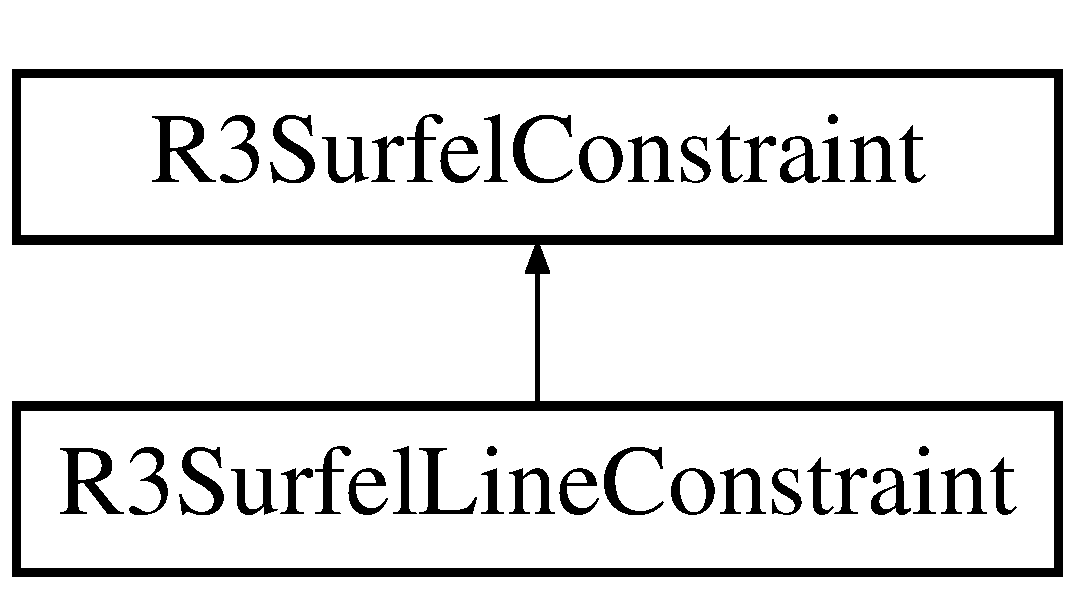
\includegraphics[height=2.000000cm]{class_r3_surfel_line_constraint}
\end{center}
\end{figure}
\subsection*{Public Member Functions}
\begin{DoxyCompactItemize}
\item 
{\bfseries R3\+Surfel\+Line\+Constraint} (const \hyperlink{class_r3_line}{R3\+Line} \&line, R\+N\+Length tolerance=0)\hypertarget{class_r3_surfel_line_constraint_a9ba4394eb63280cedf9285d16dba46ec}{}\label{class_r3_surfel_line_constraint_a9ba4394eb63280cedf9285d16dba46ec}

\item 
virtual int {\bfseries Check} (const \hyperlink{class_r3_point}{R3\+Point} \&point) const \hypertarget{class_r3_surfel_line_constraint_af1defba766c81b2fbee8f981be41e4e9}{}\label{class_r3_surfel_line_constraint_af1defba766c81b2fbee8f981be41e4e9}

\item 
virtual int {\bfseries Check} (const \hyperlink{class_r3_box}{R3\+Box} \&\hyperlink{structbox}{box}) const \hypertarget{class_r3_surfel_line_constraint_a6729a1ce89fc069e3e4e7794c0c3c7d6}{}\label{class_r3_surfel_line_constraint_a6729a1ce89fc069e3e4e7794c0c3c7d6}

\end{DoxyCompactItemize}


The documentation for this class was generated from the following files\+:\begin{DoxyCompactItemize}
\item 
R3\+Surfels/R3\+Surfel\+Constraint.\+h\item 
R3\+Surfels/R3\+Surfel\+Constraint.\+cpp\end{DoxyCompactItemize}

\hypertarget{class_r3_surfel_mark_constraint}{}\section{R3\+Surfel\+Mark\+Constraint Class Reference}
\label{class_r3_surfel_mark_constraint}\index{R3\+Surfel\+Mark\+Constraint@{R3\+Surfel\+Mark\+Constraint}}
Inheritance diagram for R3\+Surfel\+Mark\+Constraint\+:\begin{figure}[H]
\begin{center}
\leavevmode
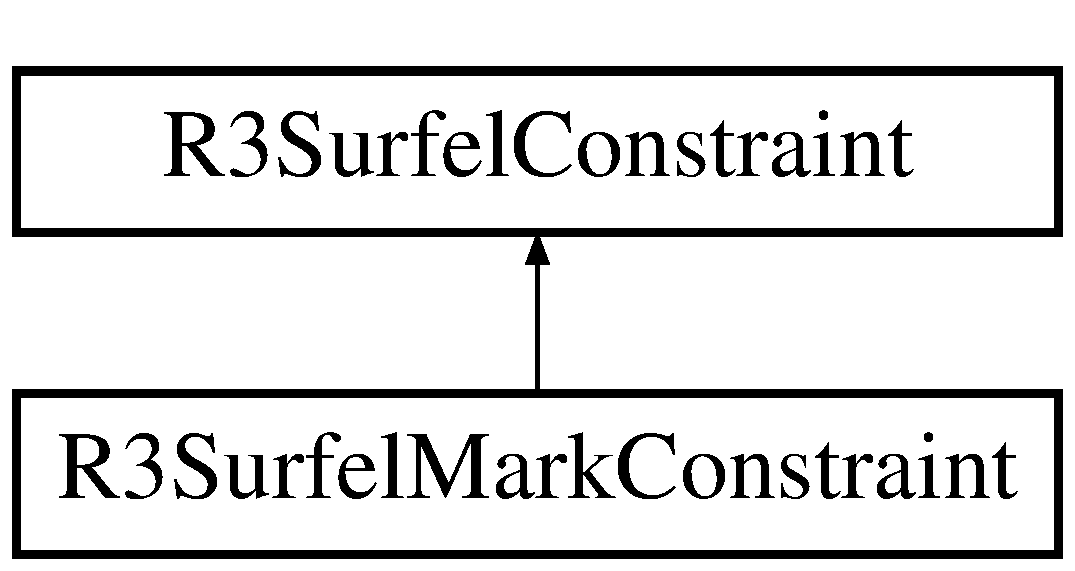
\includegraphics[height=2.000000cm]{class_r3_surfel_mark_constraint}
\end{center}
\end{figure}
\subsection*{Public Member Functions}
\begin{DoxyCompactItemize}
\item 
{\bfseries R3\+Surfel\+Mark\+Constraint} (R\+N\+Boolean include\+\_\+marked=T\+R\+UE, R\+N\+Boolean include\+\_\+unmarked=F\+A\+L\+SE)\hypertarget{class_r3_surfel_mark_constraint_aa2f3e814e1c7a44b083260aa28946b5e}{}\label{class_r3_surfel_mark_constraint_aa2f3e814e1c7a44b083260aa28946b5e}

\item 
virtual int {\bfseries Check} (const \hyperlink{class_r3_surfel_block}{R3\+Surfel\+Block} $\ast$block) const \hypertarget{class_r3_surfel_mark_constraint_aaf1d905f4d30301ce91b3da0432a8f66}{}\label{class_r3_surfel_mark_constraint_aaf1d905f4d30301ce91b3da0432a8f66}

\item 
virtual int {\bfseries Check} (const \hyperlink{class_r3_surfel_block}{R3\+Surfel\+Block} $\ast$block, const \hyperlink{class_r3_surfel}{R3\+Surfel} $\ast$surfel) const \hypertarget{class_r3_surfel_mark_constraint_aab0b25bdb8912452c8083eebf0c35df6}{}\label{class_r3_surfel_mark_constraint_aab0b25bdb8912452c8083eebf0c35df6}

\end{DoxyCompactItemize}


The documentation for this class was generated from the following files\+:\begin{DoxyCompactItemize}
\item 
R3\+Surfels/R3\+Surfel\+Constraint.\+h\item 
R3\+Surfels/R3\+Surfel\+Constraint.\+cpp\end{DoxyCompactItemize}

\hypertarget{class_r3_surfel_mesh_constraint}{}\section{R3\+Surfel\+Mesh\+Constraint Class Reference}
\label{class_r3_surfel_mesh_constraint}\index{R3\+Surfel\+Mesh\+Constraint@{R3\+Surfel\+Mesh\+Constraint}}
Inheritance diagram for R3\+Surfel\+Mesh\+Constraint\+:\begin{figure}[H]
\begin{center}
\leavevmode
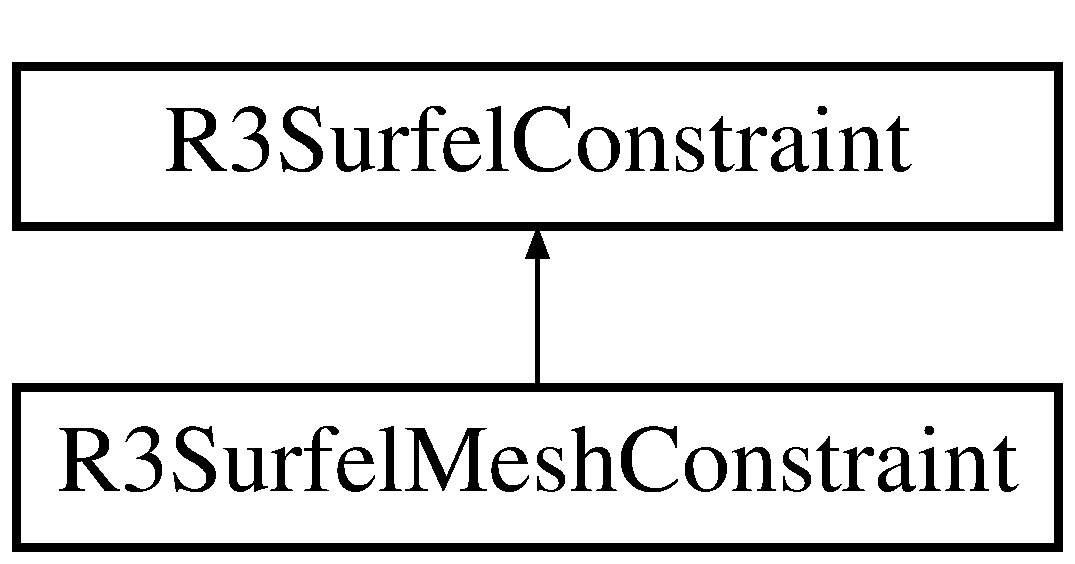
\includegraphics[height=2.000000cm]{class_r3_surfel_mesh_constraint}
\end{center}
\end{figure}
\subsection*{Public Member Functions}
\begin{DoxyCompactItemize}
\item 
{\bfseries R3\+Surfel\+Mesh\+Constraint} (\hyperlink{class_r3_mesh}{R3\+Mesh} $\ast$mesh, const \hyperlink{class_r3_affine}{R3\+Affine} \&surfels\+\_\+to\+\_\+mesh, R\+N\+Length max\+\_\+distance=0.\+25)\hypertarget{class_r3_surfel_mesh_constraint_ac90a12721551d30e96f2f962b23feef0}{}\label{class_r3_surfel_mesh_constraint_ac90a12721551d30e96f2f962b23feef0}

\item 
virtual int {\bfseries Check} (const \hyperlink{class_r3_point}{R3\+Point} \&point) const \hypertarget{class_r3_surfel_mesh_constraint_ac6685f7355d4a6e65904dd2947d7855d}{}\label{class_r3_surfel_mesh_constraint_ac6685f7355d4a6e65904dd2947d7855d}

\item 
virtual int {\bfseries Check} (const \hyperlink{class_r3_box}{R3\+Box} \&\hyperlink{structbox}{box}) const \hypertarget{class_r3_surfel_mesh_constraint_adce5786e323257464ce27667e852427c}{}\label{class_r3_surfel_mesh_constraint_adce5786e323257464ce27667e852427c}

\end{DoxyCompactItemize}


The documentation for this class was generated from the following files\+:\begin{DoxyCompactItemize}
\item 
R3\+Surfels/R3\+Surfel\+Constraint.\+h\item 
R3\+Surfels/R3\+Surfel\+Constraint.\+cpp\end{DoxyCompactItemize}

\hypertarget{class_r3_surfel_multi_constraint}{}\section{R3\+Surfel\+Multi\+Constraint Class Reference}
\label{class_r3_surfel_multi_constraint}\index{R3\+Surfel\+Multi\+Constraint@{R3\+Surfel\+Multi\+Constraint}}
Inheritance diagram for R3\+Surfel\+Multi\+Constraint\+:\begin{figure}[H]
\begin{center}
\leavevmode
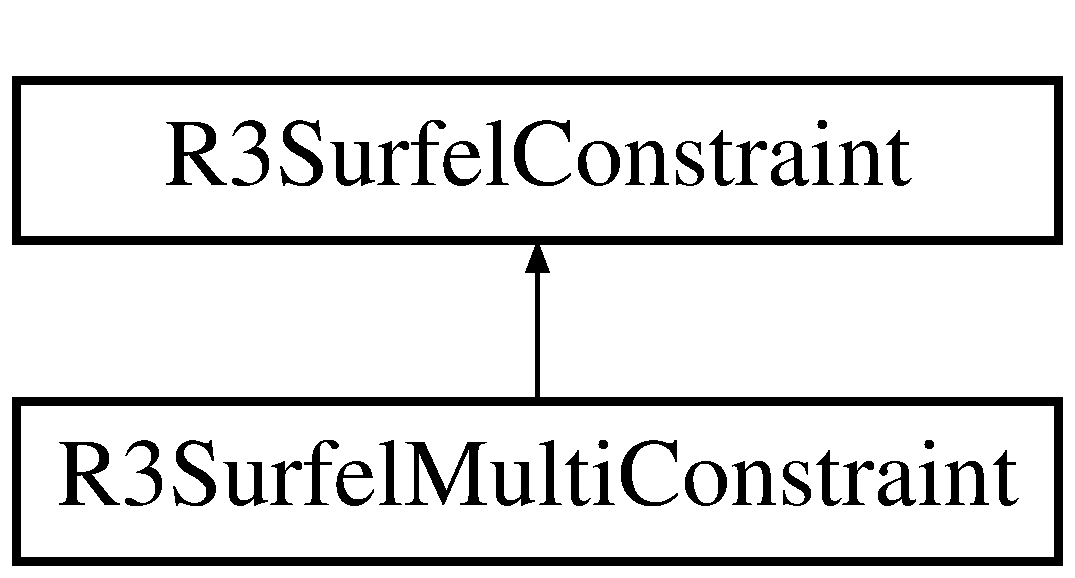
\includegraphics[height=2.000000cm]{class_r3_surfel_multi_constraint}
\end{center}
\end{figure}
\subsection*{Public Member Functions}
\begin{DoxyCompactItemize}
\item 
void {\bfseries Insert\+Constraint} (const \hyperlink{class_r3_surfel_constraint}{R3\+Surfel\+Constraint} $\ast$constraint)\hypertarget{class_r3_surfel_multi_constraint_a3d5ef6ca763be09bf0d56a9abb7b273c}{}\label{class_r3_surfel_multi_constraint_a3d5ef6ca763be09bf0d56a9abb7b273c}

\item 
void {\bfseries Remove\+Constraint} (const \hyperlink{class_r3_surfel_constraint}{R3\+Surfel\+Constraint} $\ast$constraint)\hypertarget{class_r3_surfel_multi_constraint_ae770e62a164e8f2b05e0426602fafcd8}{}\label{class_r3_surfel_multi_constraint_ae770e62a164e8f2b05e0426602fafcd8}

\item 
virtual int {\bfseries Check} (const \hyperlink{class_r3_surfel_object}{R3\+Surfel\+Object} $\ast$object) const \hypertarget{class_r3_surfel_multi_constraint_a0e63ecd36cdb630e5d6344bb5b828772}{}\label{class_r3_surfel_multi_constraint_a0e63ecd36cdb630e5d6344bb5b828772}

\item 
virtual int {\bfseries Check} (const \hyperlink{class_r3_surfel_node}{R3\+Surfel\+Node} $\ast$node) const \hypertarget{class_r3_surfel_multi_constraint_a7cb74059169c48d07e2eae38efea7d27}{}\label{class_r3_surfel_multi_constraint_a7cb74059169c48d07e2eae38efea7d27}

\item 
virtual int {\bfseries Check} (const \hyperlink{class_r3_surfel_block}{R3\+Surfel\+Block} $\ast$block) const \hypertarget{class_r3_surfel_multi_constraint_a7746059fedbc42ae85bda0559ea3c006}{}\label{class_r3_surfel_multi_constraint_a7746059fedbc42ae85bda0559ea3c006}

\item 
virtual int {\bfseries Check} (const \hyperlink{class_r3_surfel_block}{R3\+Surfel\+Block} $\ast$block, const \hyperlink{class_r3_surfel}{R3\+Surfel} $\ast$surfel) const \hypertarget{class_r3_surfel_multi_constraint_a5a451774cee42a9d409db6e1f6061aca}{}\label{class_r3_surfel_multi_constraint_a5a451774cee42a9d409db6e1f6061aca}

\item 
virtual int {\bfseries Check} (const \hyperlink{class_r3_box}{R3\+Box} \&\hyperlink{structbox}{box}) const \hypertarget{class_r3_surfel_multi_constraint_aea89a3a6867d06287331722b27a8d3b6}{}\label{class_r3_surfel_multi_constraint_aea89a3a6867d06287331722b27a8d3b6}

\item 
virtual int {\bfseries Check} (const \hyperlink{class_r3_point}{R3\+Point} \&point) const \hypertarget{class_r3_surfel_multi_constraint_a3ed679ce14135b3424c6de548be8ef39}{}\label{class_r3_surfel_multi_constraint_a3ed679ce14135b3424c6de548be8ef39}

\end{DoxyCompactItemize}


The documentation for this class was generated from the following files\+:\begin{DoxyCompactItemize}
\item 
R3\+Surfels/R3\+Surfel\+Constraint.\+h\item 
R3\+Surfels/R3\+Surfel\+Constraint.\+cpp\end{DoxyCompactItemize}

\hypertarget{class_r3_surfel_node}{}\section{R3\+Surfel\+Node Class Reference}
\label{class_r3_surfel_node}\index{R3\+Surfel\+Node@{R3\+Surfel\+Node}}
\subsection*{Public Member Functions}
\begin{DoxyCompactItemize}
\item 
{\bfseries R3\+Surfel\+Node} (const char $\ast$name=N\+U\+LL)\hypertarget{class_r3_surfel_node_a9b8980d35302d714e54a9781a91213cd}{}\label{class_r3_surfel_node_a9b8980d35302d714e54a9781a91213cd}

\item 
{\bfseries R3\+Surfel\+Node} (const \hyperlink{class_r3_surfel_node}{R3\+Surfel\+Node} \&node)\hypertarget{class_r3_surfel_node_a23c025b263d30124fa5559932de6dca1}{}\label{class_r3_surfel_node_a23c025b263d30124fa5559932de6dca1}

\item 
R\+N\+Scalar {\bfseries Complexity} (void) const \hypertarget{class_r3_surfel_node_a1134c841f459e681b96238ce18221ace}{}\label{class_r3_surfel_node_a1134c841f459e681b96238ce18221ace}

\item 
R\+N\+Scalar {\bfseries Resolution} (void) const \hypertarget{class_r3_surfel_node_a20a65fc2c069c097bb93b36f1df82736}{}\label{class_r3_surfel_node_a20a65fc2c069c097bb93b36f1df82736}

\item 
R\+N\+Scalar {\bfseries Average\+Radius} (void) const \hypertarget{class_r3_surfel_node_a2980cc8915c18b36bfe1630627e2cb94}{}\label{class_r3_surfel_node_a2980cc8915c18b36bfe1630627e2cb94}

\item 
const \hyperlink{class_r3_box}{R3\+Box} \& {\bfseries B\+Box} (void) const \hypertarget{class_r3_surfel_node_a968b610104734e16cea37904df104367}{}\label{class_r3_surfel_node_a968b610104734e16cea37904df104367}

\item 
\hyperlink{class_r3_point}{R3\+Point} {\bfseries Centroid} (void) const \hypertarget{class_r3_surfel_node_acdee894bbcfc00d3fc071ff698162e13}{}\label{class_r3_surfel_node_acdee894bbcfc00d3fc071ff698162e13}

\item 
R\+N\+Boolean {\bfseries Has\+Active} (void) const \hypertarget{class_r3_surfel_node_a2e514321e41f0c0b86de1abf517e21d0}{}\label{class_r3_surfel_node_a2e514321e41f0c0b86de1abf517e21d0}

\item 
R\+N\+Boolean {\bfseries Has\+Normals} (void) const \hypertarget{class_r3_surfel_node_ab56e99bddd5c9e44f9ef29a292e36bb7}{}\label{class_r3_surfel_node_ab56e99bddd5c9e44f9ef29a292e36bb7}

\item 
R\+N\+Boolean {\bfseries Has\+Aerial} (void) const \hypertarget{class_r3_surfel_node_a5f86daa3ae678fe52eb5c49d65afe390}{}\label{class_r3_surfel_node_a5f86daa3ae678fe52eb5c49d65afe390}

\item 
R\+N\+Boolean {\bfseries Has\+Terrestrial} (void) const \hypertarget{class_r3_surfel_node_a4f8ca2dcb75846f4a94e91dfa6dc61b5}{}\label{class_r3_surfel_node_a4f8ca2dcb75846f4a94e91dfa6dc61b5}

\item 
const char $\ast$ {\bfseries Name} (void) const \hypertarget{class_r3_surfel_node_a05ab34f60f1e9677d35810e74a8d5057}{}\label{class_r3_surfel_node_a05ab34f60f1e9677d35810e74a8d5057}

\item 
void $\ast$ {\bfseries Data} (void) const \hypertarget{class_r3_surfel_node_a0a1472eb4992eeef418dc97cd4bd93ee}{}\label{class_r3_surfel_node_a0a1472eb4992eeef418dc97cd4bd93ee}

\item 
\hyperlink{class_r3_surfel_object}{R3\+Surfel\+Object} $\ast$ {\bfseries Object} (R\+N\+Boolean search\+\_\+ancestors=F\+A\+L\+SE) const \hypertarget{class_r3_surfel_node_afc3c7b3f10a644416234fbf48b070a87}{}\label{class_r3_surfel_node_afc3c7b3f10a644416234fbf48b070a87}

\item 
\hyperlink{class_r3_surfel_scan}{R3\+Surfel\+Scan} $\ast$ {\bfseries Scan} (R\+N\+Boolean search\+\_\+ancestors=T\+R\+UE) const \hypertarget{class_r3_surfel_node_a64d6b3487c2ec515b19c073026d06238}{}\label{class_r3_surfel_node_a64d6b3487c2ec515b19c073026d06238}

\item 
\hyperlink{class_r3_surfel_tree}{R3\+Surfel\+Tree} $\ast$ {\bfseries Tree} (void) const \hypertarget{class_r3_surfel_node_a47c4447d9e917649b2322760bfd80ab5}{}\label{class_r3_surfel_node_a47c4447d9e917649b2322760bfd80ab5}

\item 
int {\bfseries Tree\+Index} (void) const \hypertarget{class_r3_surfel_node_a0ce80e0496836ff71a22361e96a8733a}{}\label{class_r3_surfel_node_a0ce80e0496836ff71a22361e96a8733a}

\item 
int {\bfseries N\+Parts} (void) const \hypertarget{class_r3_surfel_node_ace07940402d0bb9320f6cd9232ed0115}{}\label{class_r3_surfel_node_ace07940402d0bb9320f6cd9232ed0115}

\item 
\hyperlink{class_r3_surfel_node}{R3\+Surfel\+Node} $\ast$ {\bfseries Part} (int k) const \hypertarget{class_r3_surfel_node_a185f84fc14296daf9289bdcc2a12db77}{}\label{class_r3_surfel_node_a185f84fc14296daf9289bdcc2a12db77}

\item 
\hyperlink{class_r3_surfel_node}{R3\+Surfel\+Node} $\ast$ {\bfseries Parent} (void) const \hypertarget{class_r3_surfel_node_a93a27fd8d99670bfb047ccfec927219c}{}\label{class_r3_surfel_node_a93a27fd8d99670bfb047ccfec927219c}

\item 
int {\bfseries Tree\+Level} (void) const \hypertarget{class_r3_surfel_node_ad5a2787fd43d0b931e6c6d678719f645}{}\label{class_r3_surfel_node_ad5a2787fd43d0b931e6c6d678719f645}

\item 
int {\bfseries N\+Blocks} (void) const \hypertarget{class_r3_surfel_node_abde41df5d65d62a49d61f40264de70ff}{}\label{class_r3_surfel_node_abde41df5d65d62a49d61f40264de70ff}

\item 
\hyperlink{class_r3_surfel_block}{R3\+Surfel\+Block} $\ast$ {\bfseries Block} (int k) const \hypertarget{class_r3_surfel_node_a53b6e9c696df16213d75f52bf8f47f33}{}\label{class_r3_surfel_node_a53b6e9c696df16213d75f52bf8f47f33}

\item 
\hyperlink{class_r3_surfel_point_set}{R3\+Surfel\+Point\+Set} $\ast$ {\bfseries Point\+Set} (R\+N\+Boolean leaf\+\_\+level=F\+A\+L\+SE) const \hypertarget{class_r3_surfel_node_ae441dd08f2c9f699bfaad8a21adc3c80}{}\label{class_r3_surfel_node_ae441dd08f2c9f699bfaad8a21adc3c80}

\item 
virtual void {\bfseries Set\+Name} (const char $\ast$name)\hypertarget{class_r3_surfel_node_abc1ff2482a829f79d616e55fda634bce}{}\label{class_r3_surfel_node_abc1ff2482a829f79d616e55fda634bce}

\item 
virtual void {\bfseries Set\+Data} (void $\ast$data)\hypertarget{class_r3_surfel_node_a73d855ef96921fe86a18dc69932812b5}{}\label{class_r3_surfel_node_a73d855ef96921fe86a18dc69932812b5}

\item 
virtual void {\bfseries Set\+Parent} (\hyperlink{class_r3_surfel_node}{R3\+Surfel\+Node} $\ast$parent)\hypertarget{class_r3_surfel_node_ae742da019ec915b07b5638f94394eea9}{}\label{class_r3_surfel_node_ae742da019ec915b07b5638f94394eea9}

\item 
virtual void {\bfseries Insert\+Block} (\hyperlink{class_r3_surfel_block}{R3\+Surfel\+Block} $\ast$block)\hypertarget{class_r3_surfel_node_ac5556452ed9efc56a147954d70a1a281}{}\label{class_r3_surfel_node_ac5556452ed9efc56a147954d70a1a281}

\item 
virtual void {\bfseries Remove\+Block} (\hyperlink{class_r3_surfel_block}{R3\+Surfel\+Block} $\ast$block)\hypertarget{class_r3_surfel_node_a09c99544c147d3b84d5bbce216a86b8b}{}\label{class_r3_surfel_node_a09c99544c147d3b84d5bbce216a86b8b}

\item 
virtual void {\bfseries Transform} (const \hyperlink{class_r3_affine}{R3\+Affine} \&transformation)\hypertarget{class_r3_surfel_node_a6c2c066b421082871876c7e362042058}{}\label{class_r3_surfel_node_a6c2c066b421082871876c7e362042058}

\item 
virtual void {\bfseries Set\+Marks} (R\+N\+Boolean mark=T\+R\+UE)\hypertarget{class_r3_surfel_node_ab94d3ebd34dffde247f5ab9592f3ec68}{}\label{class_r3_surfel_node_ab94d3ebd34dffde247f5ab9592f3ec68}

\item 
void {\bfseries Read\+Blocks} (void)\hypertarget{class_r3_surfel_node_a0d2385af7a9c74fb261335c06a940a16}{}\label{class_r3_surfel_node_a0d2385af7a9c74fb261335c06a940a16}

\item 
void {\bfseries Release\+Blocks} (void)\hypertarget{class_r3_surfel_node_a7efcbad6bd2a1490ea8ee256ef11fea3}{}\label{class_r3_surfel_node_a7efcbad6bd2a1490ea8ee256ef11fea3}

\item 
R\+N\+Boolean {\bfseries Are\+Blocks\+Resident} (void) const \hypertarget{class_r3_surfel_node_af2e7f08424a86c51014b317787d61b3f}{}\label{class_r3_surfel_node_af2e7f08424a86c51014b317787d61b3f}

\item 
virtual void {\bfseries Draw} (\hyperlink{class_r_n_flags}{R\+N\+Flags} flags=R3\+\_\+\+S\+U\+R\+F\+E\+L\+\_\+\+D\+E\+F\+A\+U\+L\+T\+\_\+\+D\+R\+A\+W\+\_\+\+F\+L\+A\+GS) const \hypertarget{class_r3_surfel_node_a26d9f74995f8a205108ae760bb55029f}{}\label{class_r3_surfel_node_a26d9f74995f8a205108ae760bb55029f}

\item 
virtual int {\bfseries Draw\+Resident\+Ancestor} (\hyperlink{class_r_n_flags}{R\+N\+Flags} flags=R3\+\_\+\+S\+U\+R\+F\+E\+L\+\_\+\+D\+E\+F\+A\+U\+L\+T\+\_\+\+D\+R\+A\+W\+\_\+\+F\+L\+A\+GS) const \hypertarget{class_r3_surfel_node_a76dd48b89f593bed9e7d5a1e47387397}{}\label{class_r3_surfel_node_a76dd48b89f593bed9e7d5a1e47387397}

\item 
virtual int {\bfseries Draw\+Resident\+Descendents} (\hyperlink{class_r_n_flags}{R\+N\+Flags} flags=R3\+\_\+\+S\+U\+R\+F\+E\+L\+\_\+\+D\+E\+F\+A\+U\+L\+T\+\_\+\+D\+R\+A\+W\+\_\+\+F\+L\+A\+GS) const \hypertarget{class_r3_surfel_node_a9c525e257538d8c88d4b95819e99e995}{}\label{class_r3_surfel_node_a9c525e257538d8c88d4b95819e99e995}

\item 
virtual void {\bfseries Print} (F\+I\+LE $\ast$fp=N\+U\+LL, const char $\ast$prefix=N\+U\+LL, const char $\ast$suffix=N\+U\+LL) const \hypertarget{class_r3_surfel_node_ae43a1498e623c058f0ab4c9f74efcc71}{}\label{class_r3_surfel_node_ae43a1498e623c058f0ab4c9f74efcc71}

\item 
void {\bfseries Update\+Properties} (void)\hypertarget{class_r3_surfel_node_aea3ba4720ac1357ca7f1da2664244e87}{}\label{class_r3_surfel_node_aea3ba4720ac1357ca7f1da2664244e87}

\end{DoxyCompactItemize}
\subsection*{Protected Member Functions}
\begin{DoxyCompactItemize}
\item 
void {\bfseries Update\+After\+Insert} (\hyperlink{class_r3_surfel_object}{R3\+Surfel\+Object} $\ast$object)\hypertarget{class_r3_surfel_node_a6fcfb673d890350d6e9e7090360b94a3}{}\label{class_r3_surfel_node_a6fcfb673d890350d6e9e7090360b94a3}

\item 
void {\bfseries Update\+Before\+Remove} (\hyperlink{class_r3_surfel_object}{R3\+Surfel\+Object} $\ast$object)\hypertarget{class_r3_surfel_node_a2bf702afbc3f134326a56f02fb3b7177}{}\label{class_r3_surfel_node_a2bf702afbc3f134326a56f02fb3b7177}

\item 
void {\bfseries Update\+After\+Insert} (\hyperlink{class_r3_surfel_scan}{R3\+Surfel\+Scan} $\ast$scan)\hypertarget{class_r3_surfel_node_a6ed2b7831c0c096fb6679a3760396ac9}{}\label{class_r3_surfel_node_a6ed2b7831c0c096fb6679a3760396ac9}

\item 
void {\bfseries Update\+Before\+Remove} (\hyperlink{class_r3_surfel_scan}{R3\+Surfel\+Scan} $\ast$scan)\hypertarget{class_r3_surfel_node_af86ca0d43248fb395620bafaec602e22}{}\label{class_r3_surfel_node_af86ca0d43248fb395620bafaec602e22}

\item 
void {\bfseries Update\+After\+Insert} (\hyperlink{class_r3_surfel_tree}{R3\+Surfel\+Tree} $\ast$tree)\hypertarget{class_r3_surfel_node_a82d578078d3c0d4089931b6828159412}{}\label{class_r3_surfel_node_a82d578078d3c0d4089931b6828159412}

\item 
void {\bfseries Update\+Before\+Remove} (\hyperlink{class_r3_surfel_tree}{R3\+Surfel\+Tree} $\ast$tree)\hypertarget{class_r3_surfel_node_ad8a9a0c3715e2aa16287374f7717ec46}{}\label{class_r3_surfel_node_ad8a9a0c3715e2aa16287374f7717ec46}

\item 
virtual void {\bfseries Update\+B\+Box} ()\hypertarget{class_r3_surfel_node_a7c78987bf8f2c4336c104c18de3965ad}{}\label{class_r3_surfel_node_a7c78987bf8f2c4336c104c18de3965ad}

\item 
virtual void {\bfseries Update\+Complexity} ()\hypertarget{class_r3_surfel_node_af828e93fe102ee91c35843dcd420a5c1}{}\label{class_r3_surfel_node_af828e93fe102ee91c35843dcd420a5c1}

\item 
virtual void {\bfseries Update\+Resolution} ()\hypertarget{class_r3_surfel_node_a73d386388488cbcc55b5c584b2137f8b}{}\label{class_r3_surfel_node_a73d386388488cbcc55b5c584b2137f8b}

\item 
virtual void {\bfseries Update\+Flags} ()\hypertarget{class_r3_surfel_node_acb57a0eca1c5f837c5ae30084031bed3}{}\label{class_r3_surfel_node_acb57a0eca1c5f837c5ae30084031bed3}

\item 
virtual void {\bfseries Update\+Surfel\+Normals} ()\hypertarget{class_r3_surfel_node_a84e837d482215d16b9c847114b1d7f92}{}\label{class_r3_surfel_node_a84e837d482215d16b9c847114b1d7f92}

\end{DoxyCompactItemize}
\subsection*{Protected Attributes}
\begin{DoxyCompactItemize}
\item 
\hyperlink{class_r3_surfel_object}{R3\+Surfel\+Object} $\ast$ {\bfseries object}\hypertarget{class_r3_surfel_node_a67730f0eef735e4390bbc0cf85a693f9}{}\label{class_r3_surfel_node_a67730f0eef735e4390bbc0cf85a693f9}

\item 
\hyperlink{class_r3_surfel_scan}{R3\+Surfel\+Scan} $\ast$ {\bfseries scan}\hypertarget{class_r3_surfel_node_a05d98fc192b743fc8b936a77646f4e6c}{}\label{class_r3_surfel_node_a05d98fc192b743fc8b936a77646f4e6c}

\item 
\hyperlink{class_r3_surfel_tree}{R3\+Surfel\+Tree} $\ast$ {\bfseries tree}\hypertarget{class_r3_surfel_node_ac1051c415aa69184e21e446375174479}{}\label{class_r3_surfel_node_ac1051c415aa69184e21e446375174479}

\item 
int {\bfseries tree\+\_\+index}\hypertarget{class_r3_surfel_node_a0fe7d63fa40cbc57e797d831532c11a7}{}\label{class_r3_surfel_node_a0fe7d63fa40cbc57e797d831532c11a7}

\item 
\hyperlink{class_r3_surfel_node}{R3\+Surfel\+Node} $\ast$ {\bfseries parent}\hypertarget{class_r3_surfel_node_ad9d41d2c7334fd0977d33e0d6b875245}{}\label{class_r3_surfel_node_ad9d41d2c7334fd0977d33e0d6b875245}

\item 
\hyperlink{class_r_n_array}{R\+N\+Array}$<$ \hyperlink{class_r3_surfel_node}{R3\+Surfel\+Node} $\ast$ $>$ {\bfseries parts}\hypertarget{class_r3_surfel_node_ac95537d932d23d212354c97aa3756602}{}\label{class_r3_surfel_node_ac95537d932d23d212354c97aa3756602}

\item 
\hyperlink{class_r_n_array}{R\+N\+Array}$<$ \hyperlink{class_r3_surfel_block}{R3\+Surfel\+Block} $\ast$ $>$ {\bfseries blocks}\hypertarget{class_r3_surfel_node_a98e5c679ab8e660a886120ea85245a58}{}\label{class_r3_surfel_node_a98e5c679ab8e660a886120ea85245a58}

\item 
R\+N\+Scalar {\bfseries complexity}\hypertarget{class_r3_surfel_node_a2e7e181db91b72ddd30a8138a32296c8}{}\label{class_r3_surfel_node_a2e7e181db91b72ddd30a8138a32296c8}

\item 
R\+N\+Scalar {\bfseries resolution}\hypertarget{class_r3_surfel_node_aeddf84f09bc2a2d77380c0351385c2f0}{}\label{class_r3_surfel_node_aeddf84f09bc2a2d77380c0351385c2f0}

\item 
\hyperlink{class_r3_box}{R3\+Box} {\bfseries bbox}\hypertarget{class_r3_surfel_node_a794d5d09424953802338b89c78e99ccc}{}\label{class_r3_surfel_node_a794d5d09424953802338b89c78e99ccc}

\item 
char $\ast$ {\bfseries name}\hypertarget{class_r3_surfel_node_afb409f688b8b141df87a90311662fcb7}{}\label{class_r3_surfel_node_afb409f688b8b141df87a90311662fcb7}

\item 
\hyperlink{class_r_n_flags}{R\+N\+Flags} {\bfseries flags}\hypertarget{class_r3_surfel_node_a3b8738e3eaf90b58153b916910fc8b38}{}\label{class_r3_surfel_node_a3b8738e3eaf90b58153b916910fc8b38}

\item 
void $\ast$ {\bfseries data}\hypertarget{class_r3_surfel_node_a81cfe67a417fb3ca0b5658441f833571}{}\label{class_r3_surfel_node_a81cfe67a417fb3ca0b5658441f833571}

\end{DoxyCompactItemize}
\subsection*{Friends}
\begin{DoxyCompactItemize}
\item 
class {\bfseries R3\+Surfel\+Scene}\hypertarget{class_r3_surfel_node_af9bb32c0eac7d1d54787bbc6b44586b6}{}\label{class_r3_surfel_node_af9bb32c0eac7d1d54787bbc6b44586b6}

\item 
class {\bfseries R3\+Surfel\+Object}\hypertarget{class_r3_surfel_node_a850b1452c6e8af94bc02cc26bd2e5fe8}{}\label{class_r3_surfel_node_a850b1452c6e8af94bc02cc26bd2e5fe8}

\item 
class {\bfseries R3\+Surfel\+Scan}\hypertarget{class_r3_surfel_node_ad2e6d52df56aae73bbfe3d0723279197}{}\label{class_r3_surfel_node_ad2e6d52df56aae73bbfe3d0723279197}

\item 
class {\bfseries R3\+Surfel\+Tree}\hypertarget{class_r3_surfel_node_afe80cf8b46036b5125f7c9280809ed48}{}\label{class_r3_surfel_node_afe80cf8b46036b5125f7c9280809ed48}

\end{DoxyCompactItemize}


The documentation for this class was generated from the following files\+:\begin{DoxyCompactItemize}
\item 
R3\+Surfels/R3\+Surfel\+Node.\+h\item 
R3\+Surfels/R3\+Surfel\+Node.\+cpp\end{DoxyCompactItemize}

\hypertarget{class_r3_surfel_node_set}{}\section{R3\+Surfel\+Node\+Set Class Reference}
\label{class_r3_surfel_node_set}\index{R3\+Surfel\+Node\+Set@{R3\+Surfel\+Node\+Set}}
\subsection*{Public Member Functions}
\begin{DoxyCompactItemize}
\item 
{\bfseries R3\+Surfel\+Node\+Set} (const \hyperlink{class_r3_surfel_node_set}{R3\+Surfel\+Node\+Set} \&set)\hypertarget{class_r3_surfel_node_set_afb711333f22599a1c5c0660bb2b5835d}{}\label{class_r3_surfel_node_set_afb711333f22599a1c5c0660bb2b5835d}

\item 
R\+N\+Scalar {\bfseries Complexity} (void) const \hypertarget{class_r3_surfel_node_set_a9145746f0df33b6be01e9bf655a80e8e}{}\label{class_r3_surfel_node_set_a9145746f0df33b6be01e9bf655a80e8e}

\item 
\hyperlink{class_r3_point}{R3\+Point} {\bfseries Centroid} (void) const \hypertarget{class_r3_surfel_node_set_a490d1cd0ab7284606ac1cc789d5c8c69}{}\label{class_r3_surfel_node_set_a490d1cd0ab7284606ac1cc789d5c8c69}

\item 
const \hyperlink{class_r3_box}{R3\+Box} \& {\bfseries B\+Box} (void) const \hypertarget{class_r3_surfel_node_set_afc524c2f320b5ce8289339d1555b3d1a}{}\label{class_r3_surfel_node_set_afc524c2f320b5ce8289339d1555b3d1a}

\item 
int {\bfseries N\+Nodes} (void) const \hypertarget{class_r3_surfel_node_set_a012f5af3e2ad24d8b9d53b9a5af41237}{}\label{class_r3_surfel_node_set_a012f5af3e2ad24d8b9d53b9a5af41237}

\item 
\hyperlink{class_r3_surfel_node}{R3\+Surfel\+Node} $\ast$ {\bfseries Node} (int k) const \hypertarget{class_r3_surfel_node_set_a5ea82a054a06946729cfb768c807ceac}{}\label{class_r3_surfel_node_set_a5ea82a054a06946729cfb768c807ceac}

\item 
\hyperlink{class_r3_surfel_node}{R3\+Surfel\+Node} $\ast$ {\bfseries operator\mbox{[}$\,$\mbox{]}} (int k) const \hypertarget{class_r3_surfel_node_set_ac2ed674a07669e6045bd8c165ab90d3e}{}\label{class_r3_surfel_node_set_ac2ed674a07669e6045bd8c165ab90d3e}

\item 
int {\bfseries Node\+Index} (\hyperlink{class_r3_surfel_node}{R3\+Surfel\+Node} $\ast$node) const \hypertarget{class_r3_surfel_node_set_a536f28ec333a413bf670cdd9d6d7717f}{}\label{class_r3_surfel_node_set_a536f28ec333a413bf670cdd9d6d7717f}

\item 
virtual void {\bfseries Insert\+Nodes} (\hyperlink{class_r3_surfel_tree}{R3\+Surfel\+Tree} $\ast$tree)\hypertarget{class_r3_surfel_node_set_ae9cc28f309311d49f91e682fd9ce6b06}{}\label{class_r3_surfel_node_set_ae9cc28f309311d49f91e682fd9ce6b06}

\item 
virtual void {\bfseries Insert\+Nodes} (\hyperlink{class_r3_surfel_tree}{R3\+Surfel\+Tree} $\ast$tree, const \hyperlink{class_r3_point}{R3\+Point} \&xycenter, R\+N\+Length xyradius, R\+N\+Coord zmin=-\/F\+L\+T\+\_\+\+M\+AX, R\+N\+Coord zmax=F\+L\+T\+\_\+\+M\+AX, R\+N\+Scalar center\+\_\+resolution=0, R\+N\+Scalar perimeter\+\_\+resolution=0, R\+N\+Scalar focus\+\_\+exponent=10)\hypertarget{class_r3_surfel_node_set_abdbe15cbf723f84d1673ea447800af6b}{}\label{class_r3_surfel_node_set_abdbe15cbf723f84d1673ea447800af6b}

\item 
virtual void {\bfseries Insert\+Nodes} (\hyperlink{class_r3_surfel_tree}{R3\+Surfel\+Tree} $\ast$tree, \hyperlink{class_r3_surfel_node}{R3\+Surfel\+Node} $\ast$node, const \hyperlink{class_r3_point}{R3\+Point} \&xycenter, R\+N\+Length xyradius, R\+N\+Coord zmin=-\/F\+L\+T\+\_\+\+M\+AX, R\+N\+Coord zmax=F\+L\+T\+\_\+\+M\+AX, R\+N\+Scalar center\+\_\+resolution=0, R\+N\+Scalar perimeter\+\_\+resolution=0, R\+N\+Scalar focus\+\_\+exponent=10)\hypertarget{class_r3_surfel_node_set_a64bfc30a1958c259a041c196c475dcb2}{}\label{class_r3_surfel_node_set_a64bfc30a1958c259a041c196c475dcb2}

\item 
virtual void {\bfseries Insert\+Node} (\hyperlink{class_r3_surfel_node}{R3\+Surfel\+Node} $\ast$node)\hypertarget{class_r3_surfel_node_set_aebc08e3077a1a52290ab2227834ef128}{}\label{class_r3_surfel_node_set_aebc08e3077a1a52290ab2227834ef128}

\item 
virtual void {\bfseries Remove\+Node} (\hyperlink{class_r3_surfel_node}{R3\+Surfel\+Node} $\ast$node)\hypertarget{class_r3_surfel_node_set_a286a1a45772626094f2280f455bc8baf}{}\label{class_r3_surfel_node_set_a286a1a45772626094f2280f455bc8baf}

\item 
virtual void {\bfseries Remove\+Node} (int k)\hypertarget{class_r3_surfel_node_set_a4809f875ada7b63cddf46a793987b235}{}\label{class_r3_surfel_node_set_a4809f875ada7b63cddf46a793987b235}

\item 
virtual void {\bfseries Empty} (void)\hypertarget{class_r3_surfel_node_set_ab0d4626cb6d097e44c777a24f2a1ac4f}{}\label{class_r3_surfel_node_set_ab0d4626cb6d097e44c777a24f2a1ac4f}

\item 
void {\bfseries Read\+Blocks} (void)\hypertarget{class_r3_surfel_node_set_addf48ba2d8d575a5b3c5e706add8ba4a}{}\label{class_r3_surfel_node_set_addf48ba2d8d575a5b3c5e706add8ba4a}

\item 
void {\bfseries Release\+Blocks} (void)\hypertarget{class_r3_surfel_node_set_a95daa02092f0799d324cbd27c27f73a7}{}\label{class_r3_surfel_node_set_a95daa02092f0799d324cbd27c27f73a7}

\item 
R\+N\+Boolean {\bfseries Are\+Blocks\+Resident} (void) const \hypertarget{class_r3_surfel_node_set_ac4588dd94911bd4c23dc096e84700bf3}{}\label{class_r3_surfel_node_set_ac4588dd94911bd4c23dc096e84700bf3}

\item 
virtual void {\bfseries Draw} (\hyperlink{class_r_n_flags}{R\+N\+Flags} flags=R3\+\_\+\+S\+U\+R\+F\+E\+L\+\_\+\+D\+E\+F\+A\+U\+L\+T\+\_\+\+D\+R\+A\+W\+\_\+\+F\+L\+A\+GS) const \hypertarget{class_r3_surfel_node_set_ae3ffea388c01c8bc2492b1d7ab010ad3}{}\label{class_r3_surfel_node_set_ae3ffea388c01c8bc2492b1d7ab010ad3}

\item 
virtual void {\bfseries Print} (F\+I\+LE $\ast$fp=N\+U\+LL, const char $\ast$prefix=N\+U\+LL, const char $\ast$suffix=N\+U\+LL) const \hypertarget{class_r3_surfel_node_set_acee253e4db3b25f52d2f887a8a0649fe}{}\label{class_r3_surfel_node_set_acee253e4db3b25f52d2f887a8a0649fe}

\end{DoxyCompactItemize}


The documentation for this class was generated from the following files\+:\begin{DoxyCompactItemize}
\item 
R3\+Surfels/R3\+Surfel\+Node\+Set.\+h\item 
R3\+Surfels/R3\+Surfel\+Node\+Set.\+cpp\end{DoxyCompactItemize}

\hypertarget{class_r3_surfel_object}{}\section{R3\+Surfel\+Object Class Reference}
\label{class_r3_surfel_object}\index{R3\+Surfel\+Object@{R3\+Surfel\+Object}}
\subsection*{Public Member Functions}
\begin{DoxyCompactItemize}
\item 
{\bfseries R3\+Surfel\+Object} (const char $\ast$name=N\+U\+LL)\hypertarget{class_r3_surfel_object_adcd52da462d6b442b8dca1fa8a1d2667}{}\label{class_r3_surfel_object_adcd52da462d6b442b8dca1fa8a1d2667}

\item 
{\bfseries R3\+Surfel\+Object} (const \hyperlink{class_r3_surfel_object}{R3\+Surfel\+Object} \&object)\hypertarget{class_r3_surfel_object_ae16a46e3eddae1b6b71ad9cadd265e61}{}\label{class_r3_surfel_object_ae16a46e3eddae1b6b71ad9cadd265e61}

\item 
const char $\ast$ {\bfseries Name} (void) const \hypertarget{class_r3_surfel_object_a68feb518d8cf1cb398023d57cce3d9dd}{}\label{class_r3_surfel_object_a68feb518d8cf1cb398023d57cce3d9dd}

\item 
int {\bfseries Identifier} (void) const \hypertarget{class_r3_surfel_object_aa9579bd1ecb5ff58747aa1c1f0bd3530}{}\label{class_r3_surfel_object_aa9579bd1ecb5ff58747aa1c1f0bd3530}

\item 
R\+N\+Scalar {\bfseries Complexity} (void) const \hypertarget{class_r3_surfel_object_a698d029785781012a6a6641dec93cb20}{}\label{class_r3_surfel_object_a698d029785781012a6a6641dec93cb20}

\item 
const \hyperlink{class_r3_box}{R3\+Box} \& {\bfseries B\+Box} (void) const \hypertarget{class_r3_surfel_object_a57fe35b1296943fb18d9826fb2f2e80a}{}\label{class_r3_surfel_object_a57fe35b1296943fb18d9826fb2f2e80a}

\item 
\hyperlink{class_r3_point}{R3\+Point} {\bfseries Centroid} (void) const \hypertarget{class_r3_surfel_object_a69a78e16937e3b634c827d18679a904b}{}\label{class_r3_surfel_object_a69a78e16937e3b634c827d18679a904b}

\item 
const \hyperlink{class_r3_surfel_feature_vector}{R3\+Surfel\+Feature\+Vector} \& {\bfseries Feature\+Vector} (void) const \hypertarget{class_r3_surfel_object_af4a26074c6e2384adcdf877f9186bf23}{}\label{class_r3_surfel_object_af4a26074c6e2384adcdf877f9186bf23}

\item 
void $\ast$ {\bfseries Data} (void) const \hypertarget{class_r3_surfel_object_a5bd5b6a2353617a7baa548b2b02e496e}{}\label{class_r3_surfel_object_a5bd5b6a2353617a7baa548b2b02e496e}

\item 
\hyperlink{class_r3_surfel_scene}{R3\+Surfel\+Scene} $\ast$ {\bfseries Scene} (void) const \hypertarget{class_r3_surfel_object_aa0402c35ba9103955ff47cd340dd9d44}{}\label{class_r3_surfel_object_aa0402c35ba9103955ff47cd340dd9d44}

\item 
int {\bfseries Scene\+Index} (void) const \hypertarget{class_r3_surfel_object_afe4db01bf37beac2c6567a237595172d}{}\label{class_r3_surfel_object_afe4db01bf37beac2c6567a237595172d}

\item 
int {\bfseries N\+Nodes} (void) const \hypertarget{class_r3_surfel_object_a79e04eb648cbc5daa4d938466e3cc6e6}{}\label{class_r3_surfel_object_a79e04eb648cbc5daa4d938466e3cc6e6}

\item 
\hyperlink{class_r3_surfel_node}{R3\+Surfel\+Node} $\ast$ {\bfseries Node} (int k) const \hypertarget{class_r3_surfel_object_a25eac52b28063d908dff284fb050fcd2}{}\label{class_r3_surfel_object_a25eac52b28063d908dff284fb050fcd2}

\item 
int {\bfseries N\+Parts} (void) const \hypertarget{class_r3_surfel_object_ad0aea807de98013f527a9d491a5cdd33}{}\label{class_r3_surfel_object_ad0aea807de98013f527a9d491a5cdd33}

\item 
\hyperlink{class_r3_surfel_object}{R3\+Surfel\+Object} $\ast$ {\bfseries Part} (int k) const \hypertarget{class_r3_surfel_object_ad4343c4c1c87474ddd493ec96a11614d}{}\label{class_r3_surfel_object_ad4343c4c1c87474ddd493ec96a11614d}

\item 
\hyperlink{class_r3_surfel_object}{R3\+Surfel\+Object} $\ast$ {\bfseries Parent} (void) const \hypertarget{class_r3_surfel_object_a2de7a3c39423f9cf13be912a0482f506}{}\label{class_r3_surfel_object_a2de7a3c39423f9cf13be912a0482f506}

\item 
int {\bfseries Part\+Hierarchy\+Level} (void) const \hypertarget{class_r3_surfel_object_ae7046f3e920f5a266e69dd278e096266}{}\label{class_r3_surfel_object_ae7046f3e920f5a266e69dd278e096266}

\item 
\hyperlink{class_r3_surfel_scan}{R3\+Surfel\+Scan} $\ast$ {\bfseries Scan} (void) const \hypertarget{class_r3_surfel_object_ad4586ca8026b40a5d775ad0c553f2a9e}{}\label{class_r3_surfel_object_ad4586ca8026b40a5d775ad0c553f2a9e}

\item 
int {\bfseries N\+Object\+Properties} (void) const \hypertarget{class_r3_surfel_object_a5464594c652c4ea177e275656064f801}{}\label{class_r3_surfel_object_a5464594c652c4ea177e275656064f801}

\item 
\hyperlink{class_r3_surfel_object_property}{R3\+Surfel\+Object\+Property} $\ast$ {\bfseries Object\+Property} (int k) const \hypertarget{class_r3_surfel_object_a9b5baa17ea777446591b3a6c30572351}{}\label{class_r3_surfel_object_a9b5baa17ea777446591b3a6c30572351}

\item 
\hyperlink{class_r3_surfel_object_property}{R3\+Surfel\+Object\+Property} $\ast$ {\bfseries Find\+Object\+Property} (int type) const \hypertarget{class_r3_surfel_object_a8b8c76589eb76ffbc5d86fd739effb9d}{}\label{class_r3_surfel_object_a8b8c76589eb76ffbc5d86fd739effb9d}

\item 
int {\bfseries N\+Object\+Relationships} (void) const \hypertarget{class_r3_surfel_object_ab213e5342cae2e7fc79c9e7e817c1f32}{}\label{class_r3_surfel_object_ab213e5342cae2e7fc79c9e7e817c1f32}

\item 
\hyperlink{class_r3_surfel_object_relationship}{R3\+Surfel\+Object\+Relationship} $\ast$ {\bfseries Object\+Relationship} (int k) const \hypertarget{class_r3_surfel_object_a75d29fb1b3ad3838c31dc72cbbfb7218}{}\label{class_r3_surfel_object_a75d29fb1b3ad3838c31dc72cbbfb7218}

\item 
int {\bfseries N\+Label\+Assignments} (void) const \hypertarget{class_r3_surfel_object_a3972ce2ba4327ea6aeecc11c4b90c6d8}{}\label{class_r3_surfel_object_a3972ce2ba4327ea6aeecc11c4b90c6d8}

\item 
\hyperlink{class_r3_surfel_label_assignment}{R3\+Surfel\+Label\+Assignment} $\ast$ {\bfseries Label\+Assignment} (int k) const \hypertarget{class_r3_surfel_object_a4d04b0c1f0aa661e7180d26608e970ba}{}\label{class_r3_surfel_object_a4d04b0c1f0aa661e7180d26608e970ba}

\item 
\hyperlink{class_r3_surfel_label_assignment}{R3\+Surfel\+Label\+Assignment} $\ast$ {\bfseries Ground\+Truth\+Label\+Assignment} (void) const \hypertarget{class_r3_surfel_object_a38db76ad1d4bcf35e8f4073215278b81}{}\label{class_r3_surfel_object_a38db76ad1d4bcf35e8f4073215278b81}

\item 
\hyperlink{class_r3_surfel_label_assignment}{R3\+Surfel\+Label\+Assignment} $\ast$ {\bfseries Human\+Label\+Assignment} (void) const \hypertarget{class_r3_surfel_object_a7ec97bf4a0f9c33c413b51f27a9945dc}{}\label{class_r3_surfel_object_a7ec97bf4a0f9c33c413b51f27a9945dc}

\item 
\hyperlink{class_r3_surfel_label_assignment}{R3\+Surfel\+Label\+Assignment} $\ast$ {\bfseries Predicted\+Label\+Assignment} (void) const \hypertarget{class_r3_surfel_object_a5263baa5813f307f3e811255a2f6ad11}{}\label{class_r3_surfel_object_a5263baa5813f307f3e811255a2f6ad11}

\item 
\hyperlink{class_r3_surfel_label_assignment}{R3\+Surfel\+Label\+Assignment} $\ast$ {\bfseries Current\+Label\+Assignment} (void) const \hypertarget{class_r3_surfel_object_ab7280dfcb43fd88739a15592a9c80153}{}\label{class_r3_surfel_object_ab7280dfcb43fd88739a15592a9c80153}

\item 
\hyperlink{class_r3_surfel_label_assignment}{R3\+Surfel\+Label\+Assignment} $\ast$ {\bfseries Best\+Label\+Assignment} (int originator) const \hypertarget{class_r3_surfel_object_a21a4778ad44350b9ba02d4ac50214b35}{}\label{class_r3_surfel_object_a21a4778ad44350b9ba02d4ac50214b35}

\item 
\hyperlink{class_r3_surfel_label}{R3\+Surfel\+Label} $\ast$ {\bfseries Ground\+Truth\+Label} (void) const \hypertarget{class_r3_surfel_object_aadd9d6fb655b264d92cac44be23754b0}{}\label{class_r3_surfel_object_aadd9d6fb655b264d92cac44be23754b0}

\item 
\hyperlink{class_r3_surfel_label}{R3\+Surfel\+Label} $\ast$ {\bfseries Human\+Label} (void) const \hypertarget{class_r3_surfel_object_ab0f0c2a41df190851e1682eb0d20e3b3}{}\label{class_r3_surfel_object_ab0f0c2a41df190851e1682eb0d20e3b3}

\item 
\hyperlink{class_r3_surfel_label}{R3\+Surfel\+Label} $\ast$ {\bfseries Predicted\+Label} (void) const \hypertarget{class_r3_surfel_object_ab5e582ada52ce9f0bce8b84613bc5ef2}{}\label{class_r3_surfel_object_ab5e582ada52ce9f0bce8b84613bc5ef2}

\item 
\hyperlink{class_r3_surfel_label}{R3\+Surfel\+Label} $\ast$ {\bfseries Current\+Label} (void) const \hypertarget{class_r3_surfel_object_ab08930265d20e79b8407f7214110d164}{}\label{class_r3_surfel_object_ab08930265d20e79b8407f7214110d164}

\item 
\hyperlink{class_r3_surfel_label}{R3\+Surfel\+Label} $\ast$ {\bfseries Best\+Label} (int originator) const \hypertarget{class_r3_surfel_object_ad0d404d7cb9674dbf4ab84d98fd9a124}{}\label{class_r3_surfel_object_ad0d404d7cb9674dbf4ab84d98fd9a124}

\item 
\hyperlink{class_r3_surfel_point_set}{R3\+Surfel\+Point\+Set} $\ast$ {\bfseries Point\+Set} (R\+N\+Boolean leaf\+\_\+level=F\+A\+L\+SE) const \hypertarget{class_r3_surfel_object_ac46219d6bc372e1c1cffd54d1286fbd5}{}\label{class_r3_surfel_object_ac46219d6bc372e1c1cffd54d1286fbd5}

\item 
virtual void {\bfseries Set\+Parent} (\hyperlink{class_r3_surfel_object}{R3\+Surfel\+Object} $\ast$parent)\hypertarget{class_r3_surfel_object_abc42d36da2a791498005b3a509041bc1}{}\label{class_r3_surfel_object_abc42d36da2a791498005b3a509041bc1}

\item 
virtual void {\bfseries Set\+Name} (const char $\ast$name)\hypertarget{class_r3_surfel_object_a5b3a5814e4f3626d08028a9579ddf820}{}\label{class_r3_surfel_object_a5b3a5814e4f3626d08028a9579ddf820}

\item 
virtual void {\bfseries Set\+Identifier} (int identifier)\hypertarget{class_r3_surfel_object_a8dc9bdf685b522f2ac47cfddd4a62be4}{}\label{class_r3_surfel_object_a8dc9bdf685b522f2ac47cfddd4a62be4}

\item 
virtual void {\bfseries Set\+Feature\+Vector} (const \hyperlink{class_r3_surfel_feature_vector}{R3\+Surfel\+Feature\+Vector} \&vector)\hypertarget{class_r3_surfel_object_aec14e7d2ff8703d8447e7c0e5d34c1dc}{}\label{class_r3_surfel_object_aec14e7d2ff8703d8447e7c0e5d34c1dc}

\item 
virtual void {\bfseries Set\+Data} (void $\ast$data)\hypertarget{class_r3_surfel_object_a3b014b400fcedbcb2ee1211fc3114caa}{}\label{class_r3_surfel_object_a3b014b400fcedbcb2ee1211fc3114caa}

\item 
void {\bfseries Insert\+Node} (\hyperlink{class_r3_surfel_node}{R3\+Surfel\+Node} $\ast$node)\hypertarget{class_r3_surfel_object_a0916593df615305393f72fdaa2344b75}{}\label{class_r3_surfel_object_a0916593df615305393f72fdaa2344b75}

\item 
void {\bfseries Remove\+Node} (\hyperlink{class_r3_surfel_node}{R3\+Surfel\+Node} $\ast$node)\hypertarget{class_r3_surfel_object_afe905d363f5b21f7e8a3ab561f744817}{}\label{class_r3_surfel_object_afe905d363f5b21f7e8a3ab561f744817}

\item 
virtual void {\bfseries Set\+Marks} (R\+N\+Boolean mark=T\+R\+UE)\hypertarget{class_r3_surfel_object_a3d35f466cca7cafb917269f63b783449}{}\label{class_r3_surfel_object_a3d35f466cca7cafb917269f63b783449}

\item 
void {\bfseries Read\+Blocks} (void)\hypertarget{class_r3_surfel_object_ac3a96e7dc237c1f0dc9b29585b4ee8f4}{}\label{class_r3_surfel_object_ac3a96e7dc237c1f0dc9b29585b4ee8f4}

\item 
void {\bfseries Release\+Blocks} (void)\hypertarget{class_r3_surfel_object_a3f963a9d90c2e53b87dec2551646300f}{}\label{class_r3_surfel_object_a3f963a9d90c2e53b87dec2551646300f}

\item 
R\+N\+Boolean {\bfseries Are\+Blocks\+Resident} (void) const \hypertarget{class_r3_surfel_object_a821746196e0017e5db7184b92eddc097}{}\label{class_r3_surfel_object_a821746196e0017e5db7184b92eddc097}

\item 
virtual void {\bfseries Draw} (\hyperlink{class_r_n_flags}{R\+N\+Flags} flags=R3\+\_\+\+S\+U\+R\+F\+E\+L\+\_\+\+D\+E\+F\+A\+U\+L\+T\+\_\+\+D\+R\+A\+W\+\_\+\+F\+L\+A\+GS) const \hypertarget{class_r3_surfel_object_aafd3a5eb4ff48aed61cc434195be9ed0}{}\label{class_r3_surfel_object_aafd3a5eb4ff48aed61cc434195be9ed0}

\item 
virtual void {\bfseries Print} (F\+I\+LE $\ast$fp=N\+U\+LL, const char $\ast$prefix=N\+U\+LL, const char $\ast$suffix=N\+U\+LL) const \hypertarget{class_r3_surfel_object_aa3b60e989766ebef39dfc2afb7a3c9b8}{}\label{class_r3_surfel_object_aa3b60e989766ebef39dfc2afb7a3c9b8}

\item 
void {\bfseries Update\+Properties} (void)\hypertarget{class_r3_surfel_object_a35407323de4b9e6f0d769044735a3185}{}\label{class_r3_surfel_object_a35407323de4b9e6f0d769044735a3185}

\item 
void {\bfseries Update\+Feature\+Vector} (void)\hypertarget{class_r3_surfel_object_afa9974f2dfe1b2c6ac663b6df17ac583}{}\label{class_r3_surfel_object_afa9974f2dfe1b2c6ac663b6df17ac583}

\item 
void {\bfseries Update\+After\+Insert\+Block} (\hyperlink{class_r3_surfel_node}{R3\+Surfel\+Node} $\ast$node, \hyperlink{class_r3_surfel_block}{R3\+Surfel\+Block} $\ast$block)\hypertarget{class_r3_surfel_object_ad614eaafeaa307cb55db132a1b9dfc32}{}\label{class_r3_surfel_object_ad614eaafeaa307cb55db132a1b9dfc32}

\item 
void {\bfseries Update\+Before\+Remove\+Block} (\hyperlink{class_r3_surfel_node}{R3\+Surfel\+Node} $\ast$node, \hyperlink{class_r3_surfel_block}{R3\+Surfel\+Block} $\ast$block)\hypertarget{class_r3_surfel_object_a737953c680f5f9d77801d2b30c1fca40}{}\label{class_r3_surfel_object_a737953c680f5f9d77801d2b30c1fca40}

\item 
void {\bfseries Update\+After\+Transform} (\hyperlink{class_r3_surfel_node}{R3\+Surfel\+Node} $\ast$node)\hypertarget{class_r3_surfel_object_a027ecda7be743397b6549767ce8aebd2}{}\label{class_r3_surfel_object_a027ecda7be743397b6549767ce8aebd2}

\end{DoxyCompactItemize}
\subsection*{Protected Member Functions}
\begin{DoxyCompactItemize}
\item 
void {\bfseries Update\+After\+Insert} (\hyperlink{class_r3_surfel_scene}{R3\+Surfel\+Scene} $\ast$scene)\hypertarget{class_r3_surfel_object_a36aee871d62a0c3285abd23476d250b8}{}\label{class_r3_surfel_object_a36aee871d62a0c3285abd23476d250b8}

\item 
void {\bfseries Update\+Before\+Remove} (\hyperlink{class_r3_surfel_scene}{R3\+Surfel\+Scene} $\ast$scene)\hypertarget{class_r3_surfel_object_ae5c3f276518cee6758bc2476539ca9e6}{}\label{class_r3_surfel_object_ae5c3f276518cee6758bc2476539ca9e6}

\item 
void {\bfseries Update\+After\+Insert\+Object\+Property} (\hyperlink{class_r3_surfel_object_property}{R3\+Surfel\+Object\+Property} $\ast$property)\hypertarget{class_r3_surfel_object_a058781cea98717586081d76ce4f81052}{}\label{class_r3_surfel_object_a058781cea98717586081d76ce4f81052}

\item 
void {\bfseries Update\+Before\+Remove\+Object\+Property} (\hyperlink{class_r3_surfel_object_property}{R3\+Surfel\+Object\+Property} $\ast$property)\hypertarget{class_r3_surfel_object_a5e30de5068e4e5156bf09207a6e6329c}{}\label{class_r3_surfel_object_a5e30de5068e4e5156bf09207a6e6329c}

\item 
void {\bfseries Update\+After\+Insert\+Object\+Relationship} (\hyperlink{class_r3_surfel_object_relationship}{R3\+Surfel\+Object\+Relationship} $\ast$relationship)\hypertarget{class_r3_surfel_object_aa1e19fa158cb4b26c07415fc681bf452}{}\label{class_r3_surfel_object_aa1e19fa158cb4b26c07415fc681bf452}

\item 
void {\bfseries Update\+Before\+Remove\+Object\+Relationship} (\hyperlink{class_r3_surfel_object_relationship}{R3\+Surfel\+Object\+Relationship} $\ast$relationship)\hypertarget{class_r3_surfel_object_a262a1d06daf8889f6c8a70344ad93de5}{}\label{class_r3_surfel_object_a262a1d06daf8889f6c8a70344ad93de5}

\item 
void {\bfseries Update\+After\+Insert\+Label\+Assignment} (\hyperlink{class_r3_surfel_label_assignment}{R3\+Surfel\+Label\+Assignment} $\ast$assignment)\hypertarget{class_r3_surfel_object_ab89c774146b2424b6ce2d08e16849c67}{}\label{class_r3_surfel_object_ab89c774146b2424b6ce2d08e16849c67}

\item 
void {\bfseries Update\+Before\+Remove\+Label\+Assignment} (\hyperlink{class_r3_surfel_label_assignment}{R3\+Surfel\+Label\+Assignment} $\ast$assignment)\hypertarget{class_r3_surfel_object_ade01b587dff4e5a409e054906bc6bc28}{}\label{class_r3_surfel_object_ade01b587dff4e5a409e054906bc6bc28}

\item 
void {\bfseries Update\+B\+Box} ()\hypertarget{class_r3_surfel_object_a5b0830924083aac6e6a5a947ce6b9868}{}\label{class_r3_surfel_object_a5b0830924083aac6e6a5a947ce6b9868}

\end{DoxyCompactItemize}
\subsection*{Protected Attributes}
\begin{DoxyCompactItemize}
\item 
\hyperlink{class_r3_surfel_scene}{R3\+Surfel\+Scene} $\ast$ {\bfseries scene}\hypertarget{class_r3_surfel_object_a2d395fb9674ba292b003107dcaa3facd}{}\label{class_r3_surfel_object_a2d395fb9674ba292b003107dcaa3facd}

\item 
int {\bfseries scene\+\_\+index}\hypertarget{class_r3_surfel_object_ac0060c71086b866753bcb7cb175e5a5f}{}\label{class_r3_surfel_object_ac0060c71086b866753bcb7cb175e5a5f}

\item 
\hyperlink{class_r3_surfel_object}{R3\+Surfel\+Object} $\ast$ {\bfseries parent}\hypertarget{class_r3_surfel_object_ae61453677e68f1c6a9eabca21d694653}{}\label{class_r3_surfel_object_ae61453677e68f1c6a9eabca21d694653}

\item 
\hyperlink{class_r_n_array}{R\+N\+Array}$<$ \hyperlink{class_r3_surfel_object}{R3\+Surfel\+Object} $\ast$ $>$ {\bfseries parts}\hypertarget{class_r3_surfel_object_ae3bf45bd87eafe3f2d35b45af01847d5}{}\label{class_r3_surfel_object_ae3bf45bd87eafe3f2d35b45af01847d5}

\item 
\hyperlink{class_r_n_array}{R\+N\+Array}$<$ \hyperlink{class_r3_surfel_object_property}{R3\+Surfel\+Object\+Property} $\ast$ $>$ {\bfseries properties}\hypertarget{class_r3_surfel_object_a3bf767f1034ab46695d04ec0e2cdee10}{}\label{class_r3_surfel_object_a3bf767f1034ab46695d04ec0e2cdee10}

\item 
\hyperlink{class_r_n_array}{R\+N\+Array}$<$ \hyperlink{class_r3_surfel_object_relationship}{R3\+Surfel\+Object\+Relationship} $\ast$ $>$ {\bfseries relationships}\hypertarget{class_r3_surfel_object_a02536001a23969228db3cfe798db8c7d}{}\label{class_r3_surfel_object_a02536001a23969228db3cfe798db8c7d}

\item 
\hyperlink{class_r_n_array}{R\+N\+Array}$<$ \hyperlink{class_r3_surfel_label_assignment}{R3\+Surfel\+Label\+Assignment} $\ast$ $>$ {\bfseries assignments}\hypertarget{class_r3_surfel_object_acbf5de5297cdb3982257148a2384cf8f}{}\label{class_r3_surfel_object_acbf5de5297cdb3982257148a2384cf8f}

\item 
\hyperlink{class_r_n_array}{R\+N\+Array}$<$ \hyperlink{class_r3_surfel_node}{R3\+Surfel\+Node} $\ast$ $>$ {\bfseries nodes}\hypertarget{class_r3_surfel_object_a8539488e499804e97cda489d16409176}{}\label{class_r3_surfel_object_a8539488e499804e97cda489d16409176}

\item 
\hyperlink{class_r3_surfel_feature_vector}{R3\+Surfel\+Feature\+Vector} {\bfseries feature\+\_\+vector}\hypertarget{class_r3_surfel_object_af288dd7af7614eb26ba3570290ee9342}{}\label{class_r3_surfel_object_af288dd7af7614eb26ba3570290ee9342}

\item 
char $\ast$ {\bfseries name}\hypertarget{class_r3_surfel_object_af5f9566ffc2519a38afcbd390ff45a89}{}\label{class_r3_surfel_object_af5f9566ffc2519a38afcbd390ff45a89}

\item 
int {\bfseries identifier}\hypertarget{class_r3_surfel_object_a3ad735a3f4a9d8b6a222821915c11392}{}\label{class_r3_surfel_object_a3ad735a3f4a9d8b6a222821915c11392}

\item 
R\+N\+Scalar {\bfseries complexity}\hypertarget{class_r3_surfel_object_a953c79b28b143eec4f0b8f5e22431c93}{}\label{class_r3_surfel_object_a953c79b28b143eec4f0b8f5e22431c93}

\item 
\hyperlink{class_r3_box}{R3\+Box} {\bfseries bbox}\hypertarget{class_r3_surfel_object_aed0e5f4987004e25c81492989b5fb3c9}{}\label{class_r3_surfel_object_aed0e5f4987004e25c81492989b5fb3c9}

\item 
void $\ast$ {\bfseries data}\hypertarget{class_r3_surfel_object_a8708ea5683dbb7430a70421e047df9fd}{}\label{class_r3_surfel_object_a8708ea5683dbb7430a70421e047df9fd}

\end{DoxyCompactItemize}
\subsection*{Friends}
\begin{DoxyCompactItemize}
\item 
class {\bfseries R3\+Surfel\+Scene}\hypertarget{class_r3_surfel_object_af9bb32c0eac7d1d54787bbc6b44586b6}{}\label{class_r3_surfel_object_af9bb32c0eac7d1d54787bbc6b44586b6}

\end{DoxyCompactItemize}


The documentation for this class was generated from the following files\+:\begin{DoxyCompactItemize}
\item 
R3\+Surfels/R3\+Surfel\+Object.\+h\item 
R3\+Surfels/R3\+Surfel\+Object.\+cpp\end{DoxyCompactItemize}

\hypertarget{class_r3_surfel_object_constraint}{}\section{R3\+Surfel\+Object\+Constraint Class Reference}
\label{class_r3_surfel_object_constraint}\index{R3\+Surfel\+Object\+Constraint@{R3\+Surfel\+Object\+Constraint}}
Inheritance diagram for R3\+Surfel\+Object\+Constraint\+:\begin{figure}[H]
\begin{center}
\leavevmode
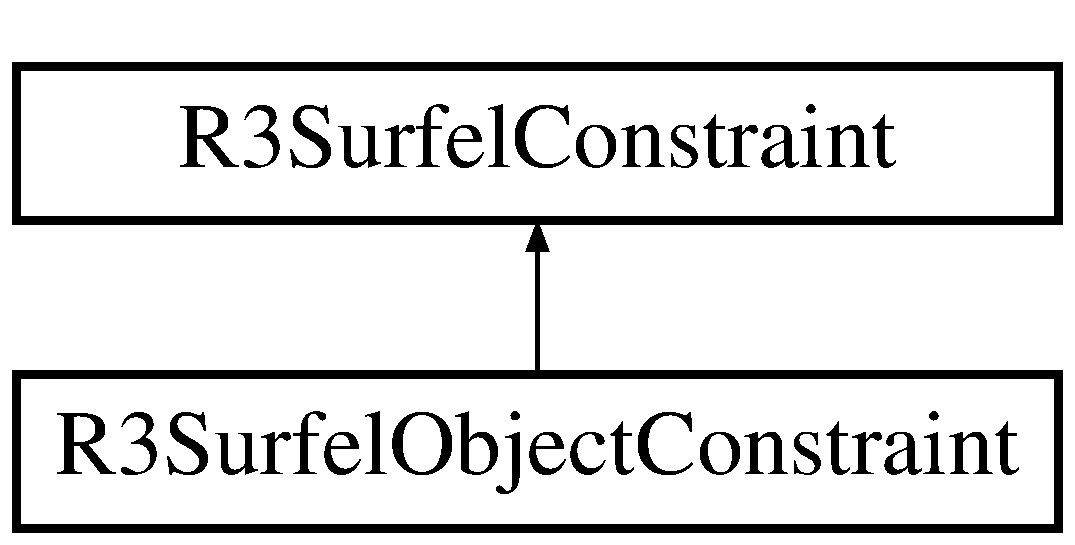
\includegraphics[height=2.000000cm]{class_r3_surfel_object_constraint}
\end{center}
\end{figure}
\subsection*{Public Member Functions}
\begin{DoxyCompactItemize}
\item 
{\bfseries R3\+Surfel\+Object\+Constraint} (\hyperlink{class_r3_surfel_object}{R3\+Surfel\+Object} $\ast$target\+\_\+object=N\+U\+LL, R\+N\+Boolean converse=F\+A\+L\+SE)\hypertarget{class_r3_surfel_object_constraint_ab1138b39986f91941dc3f2478036519b}{}\label{class_r3_surfel_object_constraint_ab1138b39986f91941dc3f2478036519b}

\item 
virtual int {\bfseries Check} (const \hyperlink{class_r3_surfel_object}{R3\+Surfel\+Object} $\ast$object) const \hypertarget{class_r3_surfel_object_constraint_a51c91233a12d115d56094ada78cc54b3}{}\label{class_r3_surfel_object_constraint_a51c91233a12d115d56094ada78cc54b3}

\item 
virtual int {\bfseries Check} (const \hyperlink{class_r3_surfel_node}{R3\+Surfel\+Node} $\ast$node) const \hypertarget{class_r3_surfel_object_constraint_a7df672b36a03e5ae88c227f09c54b5bd}{}\label{class_r3_surfel_object_constraint_a7df672b36a03e5ae88c227f09c54b5bd}

\item 
virtual int {\bfseries Check} (const \hyperlink{class_r3_surfel_block}{R3\+Surfel\+Block} $\ast$block) const \hypertarget{class_r3_surfel_object_constraint_a0d3909371a685f5b613f40f392218da2}{}\label{class_r3_surfel_object_constraint_a0d3909371a685f5b613f40f392218da2}

\item 
virtual int {\bfseries Check} (const \hyperlink{class_r3_surfel_block}{R3\+Surfel\+Block} $\ast$block, const \hyperlink{class_r3_surfel}{R3\+Surfel} $\ast$surfel) const \hypertarget{class_r3_surfel_object_constraint_a394179a6ea25b3bbbf90d36f48148725}{}\label{class_r3_surfel_object_constraint_a394179a6ea25b3bbbf90d36f48148725}

\end{DoxyCompactItemize}


The documentation for this class was generated from the following files\+:\begin{DoxyCompactItemize}
\item 
R3\+Surfels/R3\+Surfel\+Constraint.\+h\item 
R3\+Surfels/R3\+Surfel\+Constraint.\+cpp\end{DoxyCompactItemize}

\hypertarget{class_r3_surfel_object_property}{}\section{R3\+Surfel\+Object\+Property Class Reference}
\label{class_r3_surfel_object_property}\index{R3\+Surfel\+Object\+Property@{R3\+Surfel\+Object\+Property}}
\subsection*{Public Member Functions}
\begin{DoxyCompactItemize}
\item 
{\bfseries R3\+Surfel\+Object\+Property} (int type=0, \hyperlink{class_r3_surfel_object}{R3\+Surfel\+Object} $\ast$object=N\+U\+LL, R\+N\+Scalar $\ast$operands=N\+U\+LL, int noperands=0)\hypertarget{class_r3_surfel_object_property_ac87fbbbc62b53631386ea534244464bc}{}\label{class_r3_surfel_object_property_ac87fbbbc62b53631386ea534244464bc}

\item 
{\bfseries R3\+Surfel\+Object\+Property} (const \hyperlink{class_r3_surfel_object_property}{R3\+Surfel\+Object\+Property} \&property)\hypertarget{class_r3_surfel_object_property_a7095cfa3eba29d3bb1cfb7ebf2096ae0}{}\label{class_r3_surfel_object_property_a7095cfa3eba29d3bb1cfb7ebf2096ae0}

\item 
int {\bfseries Type} (void) const \hypertarget{class_r3_surfel_object_property_ad7a02acafb60c04abbd4c2981da6c0c3}{}\label{class_r3_surfel_object_property_ad7a02acafb60c04abbd4c2981da6c0c3}

\item 
\hyperlink{class_r3_surfel_scene}{R3\+Surfel\+Scene} $\ast$ {\bfseries Scene} (void) const \hypertarget{class_r3_surfel_object_property_a53e624c86b6aa2ab1120b710c8353d27}{}\label{class_r3_surfel_object_property_a53e624c86b6aa2ab1120b710c8353d27}

\item 
int {\bfseries Scene\+Index} (void) const \hypertarget{class_r3_surfel_object_property_a6040a619e28684566fbe35bcd63152f8}{}\label{class_r3_surfel_object_property_a6040a619e28684566fbe35bcd63152f8}

\item 
\hyperlink{class_r3_surfel_object}{R3\+Surfel\+Object} $\ast$ {\bfseries Object} (void) const \hypertarget{class_r3_surfel_object_property_ad4f61bfc2e9c1d5426135ccee60f2ad9}{}\label{class_r3_surfel_object_property_ad4f61bfc2e9c1d5426135ccee60f2ad9}

\item 
int {\bfseries N\+Operands} (void) const \hypertarget{class_r3_surfel_object_property_aed0a30a2d783644252cef45ee404c45e}{}\label{class_r3_surfel_object_property_aed0a30a2d783644252cef45ee404c45e}

\item 
R\+N\+Scalar {\bfseries Operand} (int k) const \hypertarget{class_r3_surfel_object_property_a4056db9f92bae30c2a82efd26b776f1b}{}\label{class_r3_surfel_object_property_a4056db9f92bae30c2a82efd26b776f1b}

\item 
virtual void {\bfseries Draw} (\hyperlink{class_r_n_flags}{R\+N\+Flags} flags=R3\+\_\+\+S\+U\+R\+F\+E\+L\+\_\+\+D\+E\+F\+A\+U\+L\+T\+\_\+\+D\+R\+A\+W\+\_\+\+F\+L\+A\+GS) const \hypertarget{class_r3_surfel_object_property_a4a215d3e78f2d448b270ffa0844d7b58}{}\label{class_r3_surfel_object_property_a4a215d3e78f2d448b270ffa0844d7b58}

\item 
void {\bfseries Update\+Operands} (void)\hypertarget{class_r3_surfel_object_property_a125fe9018aed371aa54a6d896ad43152}{}\label{class_r3_surfel_object_property_a125fe9018aed371aa54a6d896ad43152}

\end{DoxyCompactItemize}
\subsection*{Protected Member Functions}
\begin{DoxyCompactItemize}
\item 
void {\bfseries Update\+After\+Insert} (\hyperlink{class_r3_surfel_scene}{R3\+Surfel\+Scene} $\ast$scene)\hypertarget{class_r3_surfel_object_property_aa37ae0d9993fedade0b58426c9f4cf30}{}\label{class_r3_surfel_object_property_aa37ae0d9993fedade0b58426c9f4cf30}

\item 
void {\bfseries Update\+Before\+Remove} (\hyperlink{class_r3_surfel_scene}{R3\+Surfel\+Scene} $\ast$scene)\hypertarget{class_r3_surfel_object_property_a7576113c3712ee82c16840d60f538f10}{}\label{class_r3_surfel_object_property_a7576113c3712ee82c16840d60f538f10}

\end{DoxyCompactItemize}
\subsection*{Protected Attributes}
\begin{DoxyCompactItemize}
\item 
\hyperlink{class_r3_surfel_scene}{R3\+Surfel\+Scene} $\ast$ {\bfseries scene}\hypertarget{class_r3_surfel_object_property_a42e6ec5cecdb07fa8884f1f44d4db049}{}\label{class_r3_surfel_object_property_a42e6ec5cecdb07fa8884f1f44d4db049}

\item 
int {\bfseries scene\+\_\+index}\hypertarget{class_r3_surfel_object_property_ad391cffd7ab3ca2eb7959aadc3a4225d}{}\label{class_r3_surfel_object_property_ad391cffd7ab3ca2eb7959aadc3a4225d}

\item 
\hyperlink{class_r3_surfel_object}{R3\+Surfel\+Object} $\ast$ {\bfseries object}\hypertarget{class_r3_surfel_object_property_a6acdb52c04f7ad4efe09fc6e3476672b}{}\label{class_r3_surfel_object_property_a6acdb52c04f7ad4efe09fc6e3476672b}

\item 
R\+N\+Scalar $\ast$ {\bfseries operands}\hypertarget{class_r3_surfel_object_property_a7ca6445039ecfcbf57056c1892dafed5}{}\label{class_r3_surfel_object_property_a7ca6445039ecfcbf57056c1892dafed5}

\item 
int {\bfseries noperands}\hypertarget{class_r3_surfel_object_property_a30a64c964a7ce215f49408fe82eee15e}{}\label{class_r3_surfel_object_property_a30a64c964a7ce215f49408fe82eee15e}

\item 
int {\bfseries type}\hypertarget{class_r3_surfel_object_property_ad1221a4524f7fcdc29417d16f6acd3ee}{}\label{class_r3_surfel_object_property_ad1221a4524f7fcdc29417d16f6acd3ee}

\end{DoxyCompactItemize}
\subsection*{Friends}
\begin{DoxyCompactItemize}
\item 
class {\bfseries R3\+Surfel\+Scene}\hypertarget{class_r3_surfel_object_property_af9bb32c0eac7d1d54787bbc6b44586b6}{}\label{class_r3_surfel_object_property_af9bb32c0eac7d1d54787bbc6b44586b6}

\end{DoxyCompactItemize}


The documentation for this class was generated from the following files\+:\begin{DoxyCompactItemize}
\item 
R3\+Surfels/R3\+Surfel\+Object\+Property.\+h\item 
R3\+Surfels/R3\+Surfel\+Object\+Property.\+cpp\end{DoxyCompactItemize}

\hypertarget{class_r3_surfel_object_relationship}{}\section{R3\+Surfel\+Object\+Relationship Class Reference}
\label{class_r3_surfel_object_relationship}\index{R3\+Surfel\+Object\+Relationship@{R3\+Surfel\+Object\+Relationship}}
\subsection*{Public Member Functions}
\begin{DoxyCompactItemize}
\item 
{\bfseries R3\+Surfel\+Object\+Relationship} (int type=0, \hyperlink{class_r3_surfel_object}{R3\+Surfel\+Object} $\ast$object0=N\+U\+LL, \hyperlink{class_r3_surfel_object}{R3\+Surfel\+Object} $\ast$object1=N\+U\+LL, R\+N\+Scalar $\ast$operands=N\+U\+LL, int noperands=0)\hypertarget{class_r3_surfel_object_relationship_a037c3991cd611b3d156fe8c16da7620f}{}\label{class_r3_surfel_object_relationship_a037c3991cd611b3d156fe8c16da7620f}

\item 
{\bfseries R3\+Surfel\+Object\+Relationship} (int type, const \hyperlink{class_r_n_array}{R\+N\+Array}$<$ \hyperlink{class_r3_surfel_object}{R3\+Surfel\+Object} $\ast$ $>$ \&objects, R\+N\+Scalar $\ast$operands=N\+U\+LL, int noperands=0)\hypertarget{class_r3_surfel_object_relationship_a1be8aaa17218e5fbb1504ba601016ec3}{}\label{class_r3_surfel_object_relationship_a1be8aaa17218e5fbb1504ba601016ec3}

\item 
{\bfseries R3\+Surfel\+Object\+Relationship} (const \hyperlink{class_r3_surfel_object_relationship}{R3\+Surfel\+Object\+Relationship} \&relationship)\hypertarget{class_r3_surfel_object_relationship_a94a14f93b8a847a3c2f800958746d6fa}{}\label{class_r3_surfel_object_relationship_a94a14f93b8a847a3c2f800958746d6fa}

\item 
int {\bfseries Type} (void) const \hypertarget{class_r3_surfel_object_relationship_a5f5424199965e19d18b9a4c064798e30}{}\label{class_r3_surfel_object_relationship_a5f5424199965e19d18b9a4c064798e30}

\item 
\hyperlink{class_r3_surfel_scene}{R3\+Surfel\+Scene} $\ast$ {\bfseries Scene} (void) const \hypertarget{class_r3_surfel_object_relationship_a777fb9c5c821444e5870a7d69a0b2cc9}{}\label{class_r3_surfel_object_relationship_a777fb9c5c821444e5870a7d69a0b2cc9}

\item 
int {\bfseries Scene\+Index} (void) const \hypertarget{class_r3_surfel_object_relationship_ac32b9b20ce06d599338f8050851d1440}{}\label{class_r3_surfel_object_relationship_ac32b9b20ce06d599338f8050851d1440}

\item 
int {\bfseries N\+Objects} (void) const \hypertarget{class_r3_surfel_object_relationship_a1899ffeb4f7b5e186a6fd43f7e3a31ea}{}\label{class_r3_surfel_object_relationship_a1899ffeb4f7b5e186a6fd43f7e3a31ea}

\item 
\hyperlink{class_r3_surfel_object}{R3\+Surfel\+Object} $\ast$ {\bfseries Object} (int k) const \hypertarget{class_r3_surfel_object_relationship_a326d6326f1037e09d18d50249e7e9100}{}\label{class_r3_surfel_object_relationship_a326d6326f1037e09d18d50249e7e9100}

\item 
int {\bfseries N\+Operands} (void) const \hypertarget{class_r3_surfel_object_relationship_a5c1f055f753716f8f957858a252255d8}{}\label{class_r3_surfel_object_relationship_a5c1f055f753716f8f957858a252255d8}

\item 
R\+N\+Scalar {\bfseries Operand} (int k) const \hypertarget{class_r3_surfel_object_relationship_ab8142b3111ac93789e53f3d0e8d40505}{}\label{class_r3_surfel_object_relationship_ab8142b3111ac93789e53f3d0e8d40505}

\end{DoxyCompactItemize}
\subsection*{Protected Member Functions}
\begin{DoxyCompactItemize}
\item 
void {\bfseries Update\+After\+Insert} (\hyperlink{class_r3_surfel_scene}{R3\+Surfel\+Scene} $\ast$scene)\hypertarget{class_r3_surfel_object_relationship_aef71af4fa261b1b266e31ab9c76a3341}{}\label{class_r3_surfel_object_relationship_aef71af4fa261b1b266e31ab9c76a3341}

\item 
void {\bfseries Update\+Before\+Remove} (\hyperlink{class_r3_surfel_scene}{R3\+Surfel\+Scene} $\ast$scene)\hypertarget{class_r3_surfel_object_relationship_af6eb8493d15e530c0ac28d1ecf403c47}{}\label{class_r3_surfel_object_relationship_af6eb8493d15e530c0ac28d1ecf403c47}

\item 
void {\bfseries Update\+Operands} (void)\hypertarget{class_r3_surfel_object_relationship_a233214557373574497546c48dd48dbd0}{}\label{class_r3_surfel_object_relationship_a233214557373574497546c48dd48dbd0}

\end{DoxyCompactItemize}
\subsection*{Protected Attributes}
\begin{DoxyCompactItemize}
\item 
\hyperlink{class_r3_surfel_scene}{R3\+Surfel\+Scene} $\ast$ {\bfseries scene}\hypertarget{class_r3_surfel_object_relationship_a41243390750e832ae9704d127a67cf12}{}\label{class_r3_surfel_object_relationship_a41243390750e832ae9704d127a67cf12}

\item 
int {\bfseries scene\+\_\+index}\hypertarget{class_r3_surfel_object_relationship_afdab131a845e65a4ffadc164a72a0ba6}{}\label{class_r3_surfel_object_relationship_afdab131a845e65a4ffadc164a72a0ba6}

\item 
\hyperlink{class_r_n_array}{R\+N\+Array}$<$ \hyperlink{class_r3_surfel_object}{R3\+Surfel\+Object} $\ast$ $>$ {\bfseries objects}\hypertarget{class_r3_surfel_object_relationship_a6d0b4c3be6ebea54519c27e6fe82e5a7}{}\label{class_r3_surfel_object_relationship_a6d0b4c3be6ebea54519c27e6fe82e5a7}

\item 
R\+N\+Scalar $\ast$ {\bfseries operands}\hypertarget{class_r3_surfel_object_relationship_a8f2d7d83e51b410ab6cecb2cdf5b9ada}{}\label{class_r3_surfel_object_relationship_a8f2d7d83e51b410ab6cecb2cdf5b9ada}

\item 
int {\bfseries noperands}\hypertarget{class_r3_surfel_object_relationship_acf4f643711969fe557f8989f892b9391}{}\label{class_r3_surfel_object_relationship_acf4f643711969fe557f8989f892b9391}

\item 
int {\bfseries type}\hypertarget{class_r3_surfel_object_relationship_a1ce0179d6b91874b599349a20dbdf3c6}{}\label{class_r3_surfel_object_relationship_a1ce0179d6b91874b599349a20dbdf3c6}

\end{DoxyCompactItemize}
\subsection*{Friends}
\begin{DoxyCompactItemize}
\item 
class {\bfseries R3\+Surfel\+Scene}\hypertarget{class_r3_surfel_object_relationship_af9bb32c0eac7d1d54787bbc6b44586b6}{}\label{class_r3_surfel_object_relationship_af9bb32c0eac7d1d54787bbc6b44586b6}

\end{DoxyCompactItemize}


The documentation for this class was generated from the following files\+:\begin{DoxyCompactItemize}
\item 
R3\+Surfels/R3\+Surfel\+Object\+Relationship.\+h\item 
R3\+Surfels/R3\+Surfel\+Object\+Relationship.\+cpp\end{DoxyCompactItemize}

\hypertarget{class_r3_surfel_object_set}{}\section{R3\+Surfel\+Object\+Set Class Reference}
\label{class_r3_surfel_object_set}\index{R3\+Surfel\+Object\+Set@{R3\+Surfel\+Object\+Set}}
\subsection*{Public Member Functions}
\begin{DoxyCompactItemize}
\item 
{\bfseries R3\+Surfel\+Object\+Set} (const \hyperlink{class_r3_surfel_object_set}{R3\+Surfel\+Object\+Set} \&set)\hypertarget{class_r3_surfel_object_set_aeeaccd7a4f6744bd3175cc7b6ef7d831}{}\label{class_r3_surfel_object_set_aeeaccd7a4f6744bd3175cc7b6ef7d831}

\item 
\hyperlink{class_r3_point}{R3\+Point} {\bfseries Centroid} (void) const \hypertarget{class_r3_surfel_object_set_a87b719bfc51d79caf641b2b210176506}{}\label{class_r3_surfel_object_set_a87b719bfc51d79caf641b2b210176506}

\item 
const \hyperlink{class_r3_box}{R3\+Box} \& {\bfseries B\+Box} (void) const \hypertarget{class_r3_surfel_object_set_aa081af0ba582d70892d2ff9a6b01f480}{}\label{class_r3_surfel_object_set_aa081af0ba582d70892d2ff9a6b01f480}

\item 
int {\bfseries N\+Objects} (void) const \hypertarget{class_r3_surfel_object_set_a5e2f023f024ad330b7256e97ab3df7af}{}\label{class_r3_surfel_object_set_a5e2f023f024ad330b7256e97ab3df7af}

\item 
\hyperlink{class_r3_surfel_object}{R3\+Surfel\+Object} $\ast$ {\bfseries Object} (int k) const \hypertarget{class_r3_surfel_object_set_aa05ac7fa9d9c96499b3ee1aa184a79c7}{}\label{class_r3_surfel_object_set_aa05ac7fa9d9c96499b3ee1aa184a79c7}

\item 
\hyperlink{class_r3_surfel_object}{R3\+Surfel\+Object} $\ast$ {\bfseries operator\mbox{[}$\,$\mbox{]}} (int k) const \hypertarget{class_r3_surfel_object_set_ac276113eea8e38290f1d40d210ae4034}{}\label{class_r3_surfel_object_set_ac276113eea8e38290f1d40d210ae4034}

\item 
int {\bfseries Object\+Index} (\hyperlink{class_r3_surfel_object}{R3\+Surfel\+Object} $\ast$object) const \hypertarget{class_r3_surfel_object_set_a1510c3c24c7141fb69f0d01a0f1fc0ad}{}\label{class_r3_surfel_object_set_a1510c3c24c7141fb69f0d01a0f1fc0ad}

\item 
virtual void {\bfseries Insert\+Object} (\hyperlink{class_r3_surfel_object}{R3\+Surfel\+Object} $\ast$object)\hypertarget{class_r3_surfel_object_set_abbef77fb6ec0276fee6d24918aabc8e0}{}\label{class_r3_surfel_object_set_abbef77fb6ec0276fee6d24918aabc8e0}

\item 
virtual void {\bfseries Remove\+Object} (\hyperlink{class_r3_surfel_object}{R3\+Surfel\+Object} $\ast$object)\hypertarget{class_r3_surfel_object_set_abcf1adf27e002179346e16c383a97811}{}\label{class_r3_surfel_object_set_abcf1adf27e002179346e16c383a97811}

\item 
virtual void {\bfseries Remove\+Object} (int k)\hypertarget{class_r3_surfel_object_set_ab1a3e6075af116f44370bfcbec24f6a8}{}\label{class_r3_surfel_object_set_ab1a3e6075af116f44370bfcbec24f6a8}

\item 
virtual void {\bfseries Empty} (void)\hypertarget{class_r3_surfel_object_set_a20db111fc5a2555b8610dba807222c79}{}\label{class_r3_surfel_object_set_a20db111fc5a2555b8610dba807222c79}

\item 
virtual void {\bfseries Draw} (\hyperlink{class_r_n_flags}{R\+N\+Flags} flags=R3\+\_\+\+S\+U\+R\+F\+E\+L\+\_\+\+D\+E\+F\+A\+U\+L\+T\+\_\+\+D\+R\+A\+W\+\_\+\+F\+L\+A\+GS) const \hypertarget{class_r3_surfel_object_set_aa20de2043fc5030248548f23558953f1}{}\label{class_r3_surfel_object_set_aa20de2043fc5030248548f23558953f1}

\item 
virtual void {\bfseries Print} (F\+I\+LE $\ast$fp=N\+U\+LL, const char $\ast$prefix=N\+U\+LL, const char $\ast$suffix=N\+U\+LL) const \hypertarget{class_r3_surfel_object_set_ac43f74b75fdde2f2ac59018434828bdb}{}\label{class_r3_surfel_object_set_ac43f74b75fdde2f2ac59018434828bdb}

\end{DoxyCompactItemize}


The documentation for this class was generated from the following files\+:\begin{DoxyCompactItemize}
\item 
R3\+Surfels/R3\+Surfel\+Object\+Set.\+h\item 
R3\+Surfels/R3\+Surfel\+Object\+Set.\+cpp\end{DoxyCompactItemize}

\hypertarget{class_r3_surfel_overhead_grid_constraint}{}\section{R3\+Surfel\+Overhead\+Grid\+Constraint Class Reference}
\label{class_r3_surfel_overhead_grid_constraint}\index{R3\+Surfel\+Overhead\+Grid\+Constraint@{R3\+Surfel\+Overhead\+Grid\+Constraint}}
Inheritance diagram for R3\+Surfel\+Overhead\+Grid\+Constraint\+:\begin{figure}[H]
\begin{center}
\leavevmode
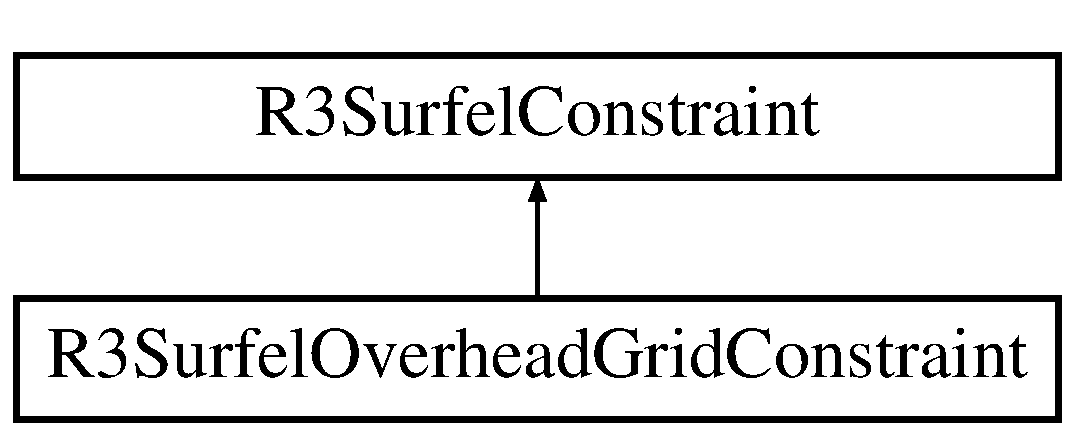
\includegraphics[height=2.000000cm]{class_r3_surfel_overhead_grid_constraint}
\end{center}
\end{figure}
\subsection*{Public Member Functions}
\begin{DoxyCompactItemize}
\item 
{\bfseries R3\+Surfel\+Overhead\+Grid\+Constraint} (const \hyperlink{class_r2_grid}{R2\+Grid} $\ast$grid, int comparison\+\_\+type=R3\+\_\+\+S\+U\+R\+F\+E\+L\+\_\+\+C\+O\+N\+S\+T\+R\+A\+I\+N\+T\+\_\+\+L\+E\+SS, int surfel\+\_\+value\+\_\+type=R3\+\_\+\+S\+U\+R\+F\+E\+L\+\_\+\+C\+O\+N\+S\+T\+R\+A\+I\+N\+T\+\_\+\+O\+P\+E\+R\+A\+ND, int grid\+\_\+value\+\_\+type=R3\+\_\+\+S\+U\+R\+F\+E\+L\+\_\+\+C\+O\+N\+S\+T\+R\+A\+I\+N\+T\+\_\+\+V\+A\+L\+UE, R\+N\+Scalar surfel\+\_\+operand=R\+N\+\_\+\+E\+P\+S\+I\+L\+ON, R\+N\+Scalar grid\+\_\+operand=0, R\+N\+Scalar epsilon=0)\hypertarget{class_r3_surfel_overhead_grid_constraint_a121e859b41e14da2819c88a1f1c773a7}{}\label{class_r3_surfel_overhead_grid_constraint_a121e859b41e14da2819c88a1f1c773a7}

\item 
virtual int {\bfseries Check} (const \hyperlink{class_r3_box}{R3\+Box} \&\hyperlink{structbox}{box}) const \hypertarget{class_r3_surfel_overhead_grid_constraint_a752c8701de975daf845fbcd8d5e98b39}{}\label{class_r3_surfel_overhead_grid_constraint_a752c8701de975daf845fbcd8d5e98b39}

\item 
virtual int {\bfseries Check} (const \hyperlink{class_r3_point}{R3\+Point} \&point) const \hypertarget{class_r3_surfel_overhead_grid_constraint_a1992a407159b8aacb0363b8f01f5dd19}{}\label{class_r3_surfel_overhead_grid_constraint_a1992a407159b8aacb0363b8f01f5dd19}

\end{DoxyCompactItemize}


The documentation for this class was generated from the following files\+:\begin{DoxyCompactItemize}
\item 
R3\+Surfels/R3\+Surfel\+Constraint.\+h\item 
R3\+Surfels/R3\+Surfel\+Constraint.\+cpp\end{DoxyCompactItemize}

\hypertarget{class_r3_surfel_overhead_grid_feature}{}\section{R3\+Surfel\+Overhead\+Grid\+Feature Class Reference}
\label{class_r3_surfel_overhead_grid_feature}\index{R3\+Surfel\+Overhead\+Grid\+Feature@{R3\+Surfel\+Overhead\+Grid\+Feature}}
Inheritance diagram for R3\+Surfel\+Overhead\+Grid\+Feature\+:\begin{figure}[H]
\begin{center}
\leavevmode
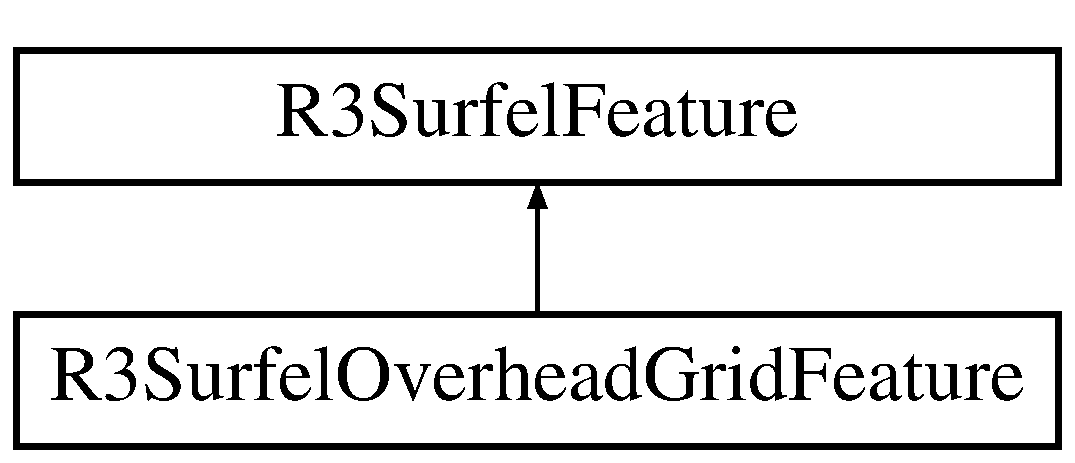
\includegraphics[height=2.000000cm]{class_r3_surfel_overhead_grid_feature}
\end{center}
\end{figure}
\subsection*{Public Member Functions}
\begin{DoxyCompactItemize}
\item 
{\bfseries R3\+Surfel\+Overhead\+Grid\+Feature} (const char $\ast$filename, const char $\ast$featurename=N\+U\+LL, R\+N\+Scalar minimum=-\/F\+L\+T\+\_\+\+M\+AX, R\+N\+Scalar maximum=F\+L\+T\+\_\+\+M\+AX, R\+N\+Scalar weight=1)\hypertarget{class_r3_surfel_overhead_grid_feature_aaf904ba9ea4bed70566fcbe90c908ba1}{}\label{class_r3_surfel_overhead_grid_feature_aaf904ba9ea4bed70566fcbe90c908ba1}

\item 
virtual int {\bfseries Type} (void) const \hypertarget{class_r3_surfel_overhead_grid_feature_a5dfd394aed57529fb2b29868b78e9d51}{}\label{class_r3_surfel_overhead_grid_feature_a5dfd394aed57529fb2b29868b78e9d51}

\item 
virtual int {\bfseries Update\+Feature\+Vector} (\hyperlink{class_r3_surfel_object}{R3\+Surfel\+Object} $\ast$object, \hyperlink{class_r3_surfel_feature_vector}{R3\+Surfel\+Feature\+Vector} \&vector) const \hypertarget{class_r3_surfel_overhead_grid_feature_a87c86ea368ff6c2ecb7587779573d45d}{}\label{class_r3_surfel_overhead_grid_feature_a87c86ea368ff6c2ecb7587779573d45d}

\end{DoxyCompactItemize}
\subsection*{Public Attributes}
\begin{DoxyCompactItemize}
\item 
char $\ast$ {\bfseries filename}\hypertarget{class_r3_surfel_overhead_grid_feature_a35103b79fd5100f7d6fad76945478122}{}\label{class_r3_surfel_overhead_grid_feature_a35103b79fd5100f7d6fad76945478122}

\item 
\hyperlink{class_r3_matrix}{R3\+Matrix} {\bfseries world\+\_\+to\+\_\+grid\+\_\+matrix}\hypertarget{class_r3_surfel_overhead_grid_feature_a83f8c5c1ee35e1c901dc0d5192e1699c}{}\label{class_r3_surfel_overhead_grid_feature_a83f8c5c1ee35e1c901dc0d5192e1699c}

\item 
int {\bfseries grid\+\_\+resolution} \mbox{[}2\mbox{]}\hypertarget{class_r3_surfel_overhead_grid_feature_ad50d240e8df44c6f2f3ee408da13283b}{}\label{class_r3_surfel_overhead_grid_feature_ad50d240e8df44c6f2f3ee408da13283b}

\item 
F\+I\+LE $\ast$ {\bfseries fp}\hypertarget{class_r3_surfel_overhead_grid_feature_aa605748497da4cc24104413d525da335}{}\label{class_r3_surfel_overhead_grid_feature_aa605748497da4cc24104413d525da335}

\end{DoxyCompactItemize}


The documentation for this class was generated from the following files\+:\begin{DoxyCompactItemize}
\item 
R3\+Surfels/R3\+Surfel\+Feature\+Evaluation.\+h\item 
R3\+Surfels/R3\+Surfel\+Feature\+Evaluation.\+cpp\end{DoxyCompactItemize}

\hypertarget{class_r3_surfel_planar_grid_constraint}{}\section{R3\+Surfel\+Planar\+Grid\+Constraint Class Reference}
\label{class_r3_surfel_planar_grid_constraint}\index{R3\+Surfel\+Planar\+Grid\+Constraint@{R3\+Surfel\+Planar\+Grid\+Constraint}}
Inheritance diagram for R3\+Surfel\+Planar\+Grid\+Constraint\+:\begin{figure}[H]
\begin{center}
\leavevmode
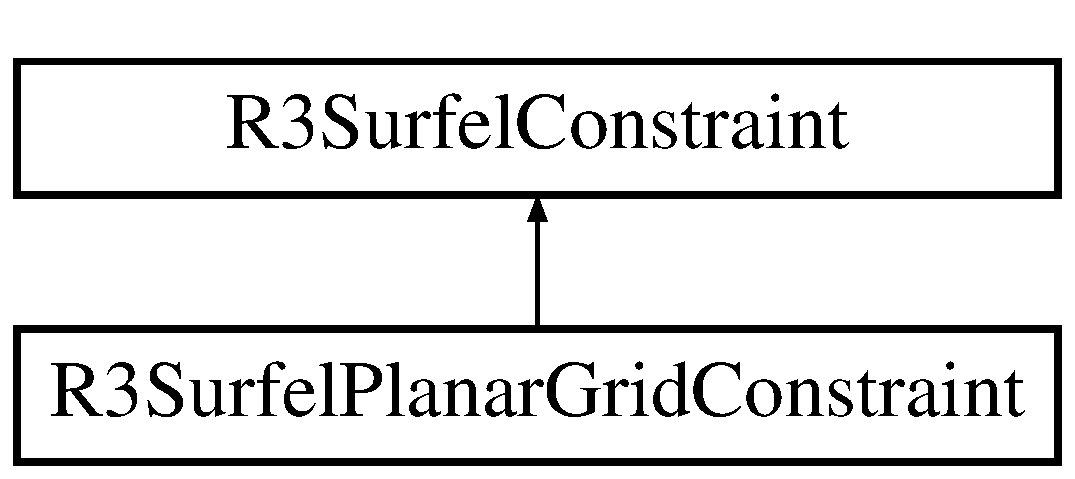
\includegraphics[height=2.000000cm]{class_r3_surfel_planar_grid_constraint}
\end{center}
\end{figure}
\subsection*{Public Member Functions}
\begin{DoxyCompactItemize}
\item 
{\bfseries R3\+Surfel\+Planar\+Grid\+Constraint} (const \hyperlink{class_r3_planar_grid}{R3\+Planar\+Grid} $\ast$grid, R\+N\+Length max\+\_\+offplane\+\_\+distance=R\+N\+\_\+\+E\+P\+S\+I\+L\+ON, int comparison\+\_\+type=R3\+\_\+\+S\+U\+R\+F\+E\+L\+\_\+\+C\+O\+N\+S\+T\+R\+A\+I\+N\+T\+\_\+\+L\+E\+SS, int surfel\+\_\+value\+\_\+type=R3\+\_\+\+S\+U\+R\+F\+E\+L\+\_\+\+C\+O\+N\+S\+T\+R\+A\+I\+N\+T\+\_\+\+O\+P\+E\+R\+A\+ND, int grid\+\_\+value\+\_\+type=R3\+\_\+\+S\+U\+R\+F\+E\+L\+\_\+\+C\+O\+N\+S\+T\+R\+A\+I\+N\+T\+\_\+\+V\+A\+L\+UE, R\+N\+Scalar surfel\+\_\+operand=R\+N\+\_\+\+E\+P\+S\+I\+L\+ON, R\+N\+Scalar grid\+\_\+operand=0, R\+N\+Scalar epsilon=0)\hypertarget{class_r3_surfel_planar_grid_constraint_a296708293604a4ecaca4e337cabb8b29}{}\label{class_r3_surfel_planar_grid_constraint_a296708293604a4ecaca4e337cabb8b29}

\item 
virtual int {\bfseries Check} (const \hyperlink{class_r3_point}{R3\+Point} \&point) const \hypertarget{class_r3_surfel_planar_grid_constraint_a6c9e82dfe4554d856f242fff3ebee09e}{}\label{class_r3_surfel_planar_grid_constraint_a6c9e82dfe4554d856f242fff3ebee09e}

\item 
virtual int {\bfseries Check} (const \hyperlink{class_r3_box}{R3\+Box} \&\hyperlink{structbox}{box}) const \hypertarget{class_r3_surfel_planar_grid_constraint_aec462c54ffecca5795a538047665e82e}{}\label{class_r3_surfel_planar_grid_constraint_aec462c54ffecca5795a538047665e82e}

\end{DoxyCompactItemize}


The documentation for this class was generated from the following files\+:\begin{DoxyCompactItemize}
\item 
R3\+Surfels/R3\+Surfel\+Constraint.\+h\item 
R3\+Surfels/R3\+Surfel\+Constraint.\+cpp\end{DoxyCompactItemize}

\hypertarget{class_r3_surfel_plane_constraint}{}\section{R3\+Surfel\+Plane\+Constraint Class Reference}
\label{class_r3_surfel_plane_constraint}\index{R3\+Surfel\+Plane\+Constraint@{R3\+Surfel\+Plane\+Constraint}}
Inheritance diagram for R3\+Surfel\+Plane\+Constraint\+:\begin{figure}[H]
\begin{center}
\leavevmode
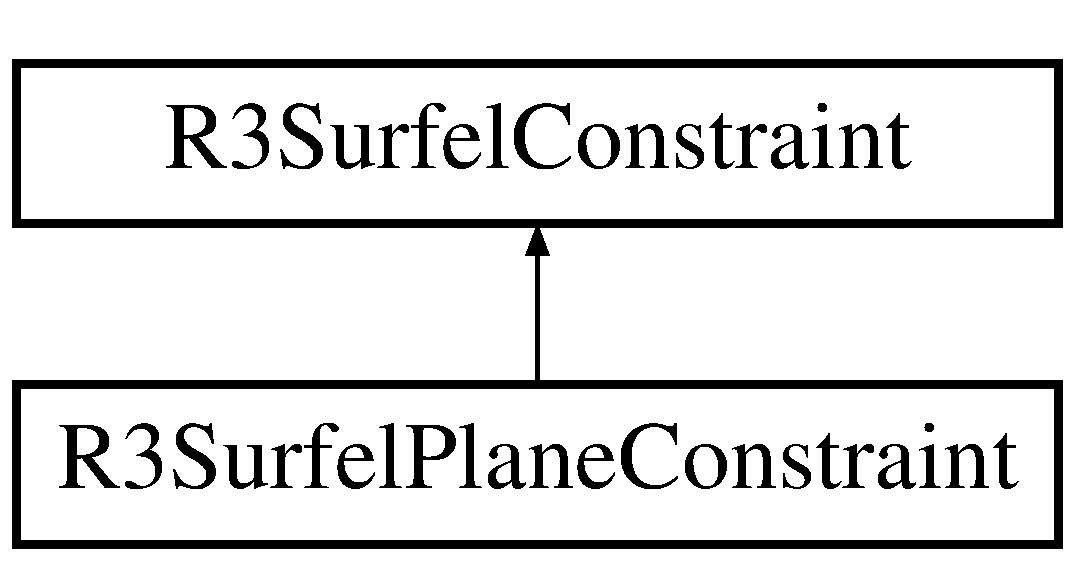
\includegraphics[height=2.000000cm]{class_r3_surfel_plane_constraint}
\end{center}
\end{figure}
\subsection*{Public Member Functions}
\begin{DoxyCompactItemize}
\item 
{\bfseries R3\+Surfel\+Plane\+Constraint} (const \hyperlink{class_r3_plane}{R3\+Plane} \&plane, R\+N\+Boolean below=T\+R\+UE, R\+N\+Boolean on=T\+R\+UE, R\+N\+Boolean above=T\+R\+UE, R\+N\+Length tolerance=0)\hypertarget{class_r3_surfel_plane_constraint_aa9df0dc135fd32ba87f8829038473119}{}\label{class_r3_surfel_plane_constraint_aa9df0dc135fd32ba87f8829038473119}

\item 
virtual int {\bfseries Check} (const \hyperlink{class_r3_point}{R3\+Point} \&point) const \hypertarget{class_r3_surfel_plane_constraint_ab2b7e2ccec1485915f84f5560c5027f3}{}\label{class_r3_surfel_plane_constraint_ab2b7e2ccec1485915f84f5560c5027f3}

\item 
virtual int {\bfseries Check} (const \hyperlink{class_r3_box}{R3\+Box} \&\hyperlink{structbox}{box}) const \hypertarget{class_r3_surfel_plane_constraint_a21e5f4c3ae15f38fcfe6623e156f152f}{}\label{class_r3_surfel_plane_constraint_a21e5f4c3ae15f38fcfe6623e156f152f}

\end{DoxyCompactItemize}


The documentation for this class was generated from the following files\+:\begin{DoxyCompactItemize}
\item 
R3\+Surfels/R3\+Surfel\+Constraint.\+h\item 
R3\+Surfels/R3\+Surfel\+Constraint.\+cpp\end{DoxyCompactItemize}

\hypertarget{class_r3_surfel_point}{}\section{R3\+Surfel\+Point Class Reference}
\label{class_r3_surfel_point}\index{R3\+Surfel\+Point@{R3\+Surfel\+Point}}
\subsection*{Public Member Functions}
\begin{DoxyCompactItemize}
\item 
{\bfseries R3\+Surfel\+Point} (const \hyperlink{class_r3_surfel_point}{R3\+Surfel\+Point} \&surfel)\hypertarget{class_r3_surfel_point_a27c769e8d26f20bdf4c060c4c34578a9}{}\label{class_r3_surfel_point_a27c769e8d26f20bdf4c060c4c34578a9}

\item 
{\bfseries R3\+Surfel\+Point} (\hyperlink{class_r3_surfel_block}{R3\+Surfel\+Block} $\ast$block, const \hyperlink{class_r3_surfel}{R3\+Surfel} $\ast$surfel)\hypertarget{class_r3_surfel_point_adb3c5f960e0d6876a15cf21664bfdb47}{}\label{class_r3_surfel_point_adb3c5f960e0d6876a15cf21664bfdb47}

\item 
R\+N\+Coord {\bfseries X} (void) const \hypertarget{class_r3_surfel_point_a01fca67786661e0f244deededeea8a88}{}\label{class_r3_surfel_point_a01fca67786661e0f244deededeea8a88}

\item 
R\+N\+Coord {\bfseries Y} (void) const \hypertarget{class_r3_surfel_point_a98c6798e5ff284741f61d68d2dc6a438}{}\label{class_r3_surfel_point_a98c6798e5ff284741f61d68d2dc6a438}

\item 
R\+N\+Coord {\bfseries Z} (void) const \hypertarget{class_r3_surfel_point_add8271d77679828e74a51ef41bfbf71c}{}\label{class_r3_surfel_point_add8271d77679828e74a51ef41bfbf71c}

\item 
R\+N\+Coord {\bfseries Coord} (int dimension) const \hypertarget{class_r3_surfel_point_a9f12364263f1aa0f30b8e6a10b5e3f22}{}\label{class_r3_surfel_point_a9f12364263f1aa0f30b8e6a10b5e3f22}

\item 
\hyperlink{class_r3_point}{R3\+Point} {\bfseries Position} (void) const \hypertarget{class_r3_surfel_point_ae7691584268e15c530c4e773a059e976}{}\label{class_r3_surfel_point_ae7691584268e15c530c4e773a059e976}

\item 
R\+N\+Coord {\bfseries NX} (void) const \hypertarget{class_r3_surfel_point_acece9cf18d6fb491c8a104f68e7d057e}{}\label{class_r3_surfel_point_acece9cf18d6fb491c8a104f68e7d057e}

\item 
R\+N\+Coord {\bfseries NY} (void) const \hypertarget{class_r3_surfel_point_a7de8498bb82d92bee8f8ca55059bc56b}{}\label{class_r3_surfel_point_a7de8498bb82d92bee8f8ca55059bc56b}

\item 
R\+N\+Coord {\bfseries NZ} (void) const \hypertarget{class_r3_surfel_point_a200ee9bd65789ac79fc51385630ebf42}{}\label{class_r3_surfel_point_a200ee9bd65789ac79fc51385630ebf42}

\item 
R\+N\+Coord {\bfseries Normal\+Coord} (int dimension) const \hypertarget{class_r3_surfel_point_a4b82b8e4fdfc3b27050826f2c8545f44}{}\label{class_r3_surfel_point_a4b82b8e4fdfc3b27050826f2c8545f44}

\item 
\hyperlink{class_r3_vector}{R3\+Vector} {\bfseries Normal} (void) const \hypertarget{class_r3_surfel_point_a9f907c4a4989157e2059440fec533c49}{}\label{class_r3_surfel_point_a9f907c4a4989157e2059440fec533c49}

\item 
float {\bfseries Radius} (void) const \hypertarget{class_r3_surfel_point_a3b311e3343ddf27434f4682c673bb5ac}{}\label{class_r3_surfel_point_a3b311e3343ddf27434f4682c673bb5ac}

\item 
unsigned char {\bfseries R} (void) const \hypertarget{class_r3_surfel_point_a32597c65d1603ec4429d39429a7d4ad8}{}\label{class_r3_surfel_point_a32597c65d1603ec4429d39429a7d4ad8}

\item 
unsigned char {\bfseries G} (void) const \hypertarget{class_r3_surfel_point_a9bb30169fcf7c318bc4865c87112e542}{}\label{class_r3_surfel_point_a9bb30169fcf7c318bc4865c87112e542}

\item 
unsigned char {\bfseries B} (void) const \hypertarget{class_r3_surfel_point_a4456abf8b87e24ebe2d1a83cbf84deee}{}\label{class_r3_surfel_point_a4456abf8b87e24ebe2d1a83cbf84deee}

\item 
const unsigned char $\ast$ {\bfseries Color} (void) const \hypertarget{class_r3_surfel_point_a78816c78ab8d4bb2aabd1b5bfeaf9e33}{}\label{class_r3_surfel_point_a78816c78ab8d4bb2aabd1b5bfeaf9e33}

\item 
\hyperlink{class_r_n_rgb}{R\+N\+Rgb} {\bfseries Rgb} (void) const \hypertarget{class_r3_surfel_point_a5f9279b18d6293c557bfe6d1f46a2cba}{}\label{class_r3_surfel_point_a5f9279b18d6293c557bfe6d1f46a2cba}

\item 
R\+N\+Boolean {\bfseries Is\+On\+Silhouette\+Boundary} (void) const \hypertarget{class_r3_surfel_point_a9aeacfe66d3d020d51c4f19dbb713a3b}{}\label{class_r3_surfel_point_a9aeacfe66d3d020d51c4f19dbb713a3b}

\item 
R\+N\+Boolean {\bfseries Is\+On\+Shadow\+Boundary} (void) const \hypertarget{class_r3_surfel_point_ae07cd41526e5bbaf94407e7bc7bbf9c3}{}\label{class_r3_surfel_point_ae07cd41526e5bbaf94407e7bc7bbf9c3}

\item 
R\+N\+Boolean {\bfseries Is\+On\+Border\+Boundary} (void) const \hypertarget{class_r3_surfel_point_afa712d892287866ce4379f37c1772e36}{}\label{class_r3_surfel_point_afa712d892287866ce4379f37c1772e36}

\item 
R\+N\+Boolean {\bfseries Is\+On\+Boundary} (void) const \hypertarget{class_r3_surfel_point_a9d947e9f78cc093035bcd3bbc8b820f7}{}\label{class_r3_surfel_point_a9d947e9f78cc093035bcd3bbc8b820f7}

\item 
R\+N\+Boolean {\bfseries Is\+Aerial} (void) const \hypertarget{class_r3_surfel_point_ae7c8572504851b48546a3d8872fc1460}{}\label{class_r3_surfel_point_ae7c8572504851b48546a3d8872fc1460}

\item 
R\+N\+Boolean {\bfseries Is\+Marked} (void) const \hypertarget{class_r3_surfel_point_ae217cbe7c5a7089d77c0eb4f81ca2ad3}{}\label{class_r3_surfel_point_ae217cbe7c5a7089d77c0eb4f81ca2ad3}

\item 
R\+N\+Boolean {\bfseries Has\+Normal} (void) const \hypertarget{class_r3_surfel_point_a0753df898f552f27b53511b24625530e}{}\label{class_r3_surfel_point_a0753df898f552f27b53511b24625530e}

\item 
\hyperlink{class_r3_surfel_block}{R3\+Surfel\+Block} $\ast$ {\bfseries Block} (void) const \hypertarget{class_r3_surfel_point_a53a9a98271226cb437ca44189fe2f7ca}{}\label{class_r3_surfel_point_a53a9a98271226cb437ca44189fe2f7ca}

\item 
int {\bfseries Block\+Index} (void) const \hypertarget{class_r3_surfel_point_a5a88a780f93969fa569f1736e400bac9}{}\label{class_r3_surfel_point_a5a88a780f93969fa569f1736e400bac9}

\item 
const \hyperlink{class_r3_surfel}{R3\+Surfel} $\ast$ {\bfseries Surfel} (void) const \hypertarget{class_r3_surfel_point_ad6dd9e18d3b9184e8011db7333875e35}{}\label{class_r3_surfel_point_ad6dd9e18d3b9184e8011db7333875e35}

\item 
void {\bfseries Copy} (const \hyperlink{class_r3_surfel_point}{R3\+Surfel\+Point} $\ast$point)\hypertarget{class_r3_surfel_point_a73f2fda7d424c47f6a4b4bb9b0f686d0}{}\label{class_r3_surfel_point_a73f2fda7d424c47f6a4b4bb9b0f686d0}

\item 
void {\bfseries Reset} (\hyperlink{class_r3_surfel_block}{R3\+Surfel\+Block} $\ast$block, const \hyperlink{class_r3_surfel}{R3\+Surfel} $\ast$surfel)\hypertarget{class_r3_surfel_point_a591509bd50199800a0dc5c9ed11ae934}{}\label{class_r3_surfel_point_a591509bd50199800a0dc5c9ed11ae934}

\item 
\hyperlink{class_r3_surfel_point}{R3\+Surfel\+Point} \& {\bfseries operator=} (const \hyperlink{class_r3_surfel_point}{R3\+Surfel\+Point} \&point)\hypertarget{class_r3_surfel_point_a7587940b081c0fa2fd4a953af9aa8687}{}\label{class_r3_surfel_point_a7587940b081c0fa2fd4a953af9aa8687}

\item 
void {\bfseries Set\+Position} (const \hyperlink{class_r3_point}{R3\+Point} \&position)\hypertarget{class_r3_surfel_point_af35ccf9413aa3c406cb32f75aff99af0}{}\label{class_r3_surfel_point_af35ccf9413aa3c406cb32f75aff99af0}

\item 
void {\bfseries Set\+Normal} (const \hyperlink{class_r3_vector}{R3\+Vector} \&normal)\hypertarget{class_r3_surfel_point_a6bb15c7fed5e8b240dd533be1db1dcb1}{}\label{class_r3_surfel_point_a6bb15c7fed5e8b240dd533be1db1dcb1}

\item 
void {\bfseries Set\+Color} (const \hyperlink{class_r_n_rgb}{R\+N\+Rgb} \&color)\hypertarget{class_r3_surfel_point_ab879f615a74a968fe305f6a7e50ecc8d}{}\label{class_r3_surfel_point_ab879f615a74a968fe305f6a7e50ecc8d}

\item 
void {\bfseries Set\+Active} (R\+N\+Boolean active=T\+R\+UE)\hypertarget{class_r3_surfel_point_acb660e9f47be931fbd114592b0a23d22}{}\label{class_r3_surfel_point_acb660e9f47be931fbd114592b0a23d22}

\item 
void {\bfseries Set\+Aerial} (R\+N\+Boolean aerial=T\+R\+UE)\hypertarget{class_r3_surfel_point_a1a4d1e8b101991e0a7768f1d39cffb38}{}\label{class_r3_surfel_point_a1a4d1e8b101991e0a7768f1d39cffb38}

\item 
void {\bfseries Set\+Mark} (R\+N\+Boolean mark)\hypertarget{class_r3_surfel_point_a7ffa68526868442273f240e262b6a245}{}\label{class_r3_surfel_point_a7ffa68526868442273f240e262b6a245}

\item 
void {\bfseries Draw} (\hyperlink{class_r_n_flags}{R\+N\+Flags} flags=R3\+\_\+\+S\+U\+R\+F\+E\+L\+\_\+\+D\+E\+F\+A\+U\+L\+T\+\_\+\+D\+R\+A\+W\+\_\+\+F\+L\+A\+GS) const \hypertarget{class_r3_surfel_point_aa3d83c5069b82f0ee71849083e4a491d}{}\label{class_r3_surfel_point_aa3d83c5069b82f0ee71849083e4a491d}

\end{DoxyCompactItemize}


The documentation for this class was generated from the following files\+:\begin{DoxyCompactItemize}
\item 
R3\+Surfels/R3\+Surfel\+Point.\+h\item 
R3\+Surfels/R3\+Surfel\+Point.\+cpp\end{DoxyCompactItemize}

\hypertarget{class_r3_surfel_point_graph}{}\section{R3\+Surfel\+Point\+Graph Class Reference}
\label{class_r3_surfel_point_graph}\index{R3\+Surfel\+Point\+Graph@{R3\+Surfel\+Point\+Graph}}
\subsection*{Public Member Functions}
\begin{DoxyCompactItemize}
\item 
{\bfseries R3\+Surfel\+Point\+Graph} (const \hyperlink{class_r3_surfel_point_graph}{R3\+Surfel\+Point\+Graph} \&graph)\hypertarget{class_r3_surfel_point_graph_a15bc00a7ab19e3b188f4c5510ebbba0f}{}\label{class_r3_surfel_point_graph_a15bc00a7ab19e3b188f4c5510ebbba0f}

\item 
{\bfseries R3\+Surfel\+Point\+Graph} (const \hyperlink{class_r3_surfel_point_set}{R3\+Surfel\+Point\+Set} \&set, int max\+\_\+neighbors=16, R\+N\+Length max\+\_\+distance=1)\hypertarget{class_r3_surfel_point_graph_a724f57279be5382f0fa55aa251d7d7b7}{}\label{class_r3_surfel_point_graph_a724f57279be5382f0fa55aa251d7d7b7}

\item 
\hyperlink{class_r3_point}{R3\+Point} {\bfseries Centroid} (void) const \hypertarget{class_r3_surfel_point_graph_a6ac2b48f66a61e5d9b67ec60f91a1ea4}{}\label{class_r3_surfel_point_graph_a6ac2b48f66a61e5d9b67ec60f91a1ea4}

\item 
const \hyperlink{class_r3_box}{R3\+Box} \& {\bfseries B\+Box} (void) const \hypertarget{class_r3_surfel_point_graph_a0b6a0c8789d64858fb830a41d5b7c12c}{}\label{class_r3_surfel_point_graph_a0b6a0c8789d64858fb830a41d5b7c12c}

\item 
int {\bfseries Max\+Neighbors} (void) const \hypertarget{class_r3_surfel_point_graph_a8d9fdbf5815e0567f0de21d26430b62c}{}\label{class_r3_surfel_point_graph_a8d9fdbf5815e0567f0de21d26430b62c}

\item 
R\+N\+Length {\bfseries Max\+Distance} (void) const \hypertarget{class_r3_surfel_point_graph_a93887396d304b38714d2f9f0bbf50af0}{}\label{class_r3_surfel_point_graph_a93887396d304b38714d2f9f0bbf50af0}

\item 
int {\bfseries N\+Points} (void) const \hypertarget{class_r3_surfel_point_graph_ad352a6a2ba9505c6d6c23bab7be79092}{}\label{class_r3_surfel_point_graph_ad352a6a2ba9505c6d6c23bab7be79092}

\item 
\hyperlink{class_r3_surfel_point}{R3\+Surfel\+Point} $\ast$ {\bfseries Point} (int k) const \hypertarget{class_r3_surfel_point_graph_a848b79d5f3a7876f0f34e7a000e2aa1e}{}\label{class_r3_surfel_point_graph_a848b79d5f3a7876f0f34e7a000e2aa1e}

\item 
\hyperlink{class_r3_surfel_point}{R3\+Surfel\+Point} $\ast$ {\bfseries operator\mbox{[}$\,$\mbox{]}} (int k) const \hypertarget{class_r3_surfel_point_graph_a217e226166421fbc0a489f0b78fad694}{}\label{class_r3_surfel_point_graph_a217e226166421fbc0a489f0b78fad694}

\item 
int {\bfseries N\+Neighbors} (int surfel\+\_\+index) const \hypertarget{class_r3_surfel_point_graph_ace9965d96f7771ab46f197f5237af7a5}{}\label{class_r3_surfel_point_graph_ace9965d96f7771ab46f197f5237af7a5}

\item 
\hyperlink{class_r3_surfel_point}{R3\+Surfel\+Point} $\ast$ {\bfseries Neighbor} (int surfel\+\_\+index, int neighbor\+\_\+index) const \hypertarget{class_r3_surfel_point_graph_a0da3982a56e64a25dcd3865ff85d7b1f}{}\label{class_r3_surfel_point_graph_a0da3982a56e64a25dcd3865ff85d7b1f}

\item 
int {\bfseries Point\+Index} (const \hyperlink{class_r3_surfel_point}{R3\+Surfel\+Point} $\ast$point) const \hypertarget{class_r3_surfel_point_graph_a134fc6741162e804e7eab17d76e27db8}{}\label{class_r3_surfel_point_graph_a134fc6741162e804e7eab17d76e27db8}

\item 
\hyperlink{class_r3_vector}{R3\+Vector} {\bfseries Point\+Normal} (const \hyperlink{class_r3_surfel_point}{R3\+Surfel\+Point} $\ast$point, R\+N\+Boolean fast\+\_\+and\+\_\+approximate=F\+A\+L\+SE) const \hypertarget{class_r3_surfel_point_graph_ab2831049499e488fa2723e35b420753d}{}\label{class_r3_surfel_point_graph_ab2831049499e488fa2723e35b420753d}

\item 
\hyperlink{class_r3_vector}{R3\+Vector} {\bfseries Point\+Normal} (int point\+\_\+index, R\+N\+Boolean fast\+\_\+and\+\_\+approximate=F\+A\+L\+SE) const \hypertarget{class_r3_surfel_point_graph_a977123db921465b265cc2209cd60ad7f}{}\label{class_r3_surfel_point_graph_a977123db921465b265cc2209cd60ad7f}

\item 
void {\bfseries Set\+Marks} (R\+N\+Boolean mark)\hypertarget{class_r3_surfel_point_graph_aa2f62a27df36042a75f0859605bf45d7}{}\label{class_r3_surfel_point_graph_aa2f62a27df36042a75f0859605bf45d7}

\item 
virtual void {\bfseries Draw} (\hyperlink{class_r_n_flags}{R\+N\+Flags} flags=R3\+\_\+\+S\+U\+R\+F\+E\+L\+\_\+\+D\+E\+F\+A\+U\+L\+T\+\_\+\+D\+R\+A\+W\+\_\+\+F\+L\+A\+GS) const \hypertarget{class_r3_surfel_point_graph_a81ed66885f630f46034dd3a7bcf2e1dd}{}\label{class_r3_surfel_point_graph_a81ed66885f630f46034dd3a7bcf2e1dd}

\item 
void {\bfseries Update\+Normals} (void) const \hypertarget{class_r3_surfel_point_graph_ab0ce15371513da48de1da0a8e97ccc09}{}\label{class_r3_surfel_point_graph_ab0ce15371513da48de1da0a8e97ccc09}

\item 
void {\bfseries Remove\+Outlier\+Edges} (R\+N\+Scalar zscore)\hypertarget{class_r3_surfel_point_graph_ac95a66a3c71ce0e61d234d29a1d3ebdb}{}\label{class_r3_surfel_point_graph_ac95a66a3c71ce0e61d234d29a1d3ebdb}

\end{DoxyCompactItemize}


The documentation for this class was generated from the following files\+:\begin{DoxyCompactItemize}
\item 
R3\+Surfels/R3\+Surfel\+Point\+Graph.\+h\item 
R3\+Surfels/R3\+Surfel\+Point\+Graph.\+cpp\end{DoxyCompactItemize}

\hypertarget{class_r3_surfel_point_set}{}\section{R3\+Surfel\+Point\+Set Class Reference}
\label{class_r3_surfel_point_set}\index{R3\+Surfel\+Point\+Set@{R3\+Surfel\+Point\+Set}}
\subsection*{Public Member Functions}
\begin{DoxyCompactItemize}
\item 
{\bfseries R3\+Surfel\+Point\+Set} (const \hyperlink{class_r3_surfel_point_set}{R3\+Surfel\+Point\+Set} \&set)\hypertarget{class_r3_surfel_point_set_aca27752edf5a20cb006bf2dd861d1ab7}{}\label{class_r3_surfel_point_set_aca27752edf5a20cb006bf2dd861d1ab7}

\item 
{\bfseries R3\+Surfel\+Point\+Set} (\hyperlink{class_r3_surfel_block}{R3\+Surfel\+Block} $\ast$block)\hypertarget{class_r3_surfel_point_set_a9202a9eb38944c936e6d5f233705d796}{}\label{class_r3_surfel_point_set_a9202a9eb38944c936e6d5f233705d796}

\item 
int {\bfseries N\+Points} (void) const \hypertarget{class_r3_surfel_point_set_ac24ae72dd6326f14c0cb5fcd57b3e8f0}{}\label{class_r3_surfel_point_set_ac24ae72dd6326f14c0cb5fcd57b3e8f0}

\item 
\hyperlink{class_r3_surfel_point}{R3\+Surfel\+Point} $\ast$ {\bfseries Point} (int k) const \hypertarget{class_r3_surfel_point_set_ac87fb27059c215f5292333df2b1ce216}{}\label{class_r3_surfel_point_set_ac87fb27059c215f5292333df2b1ce216}

\item 
\hyperlink{class_r3_surfel_point}{R3\+Surfel\+Point} $\ast$ {\bfseries operator\mbox{[}$\,$\mbox{]}} (int k) const \hypertarget{class_r3_surfel_point_set_a5bc3bf24d795fad638543c7e64cc6a9a}{}\label{class_r3_surfel_point_set_a5bc3bf24d795fad638543c7e64cc6a9a}

\item 
int {\bfseries Point\+Index} (const \hyperlink{class_r3_surfel_point}{R3\+Surfel\+Point} $\ast$point) const \hypertarget{class_r3_surfel_point_set_abaa764e9be10a61cc9b8fb5842a25212}{}\label{class_r3_surfel_point_set_abaa764e9be10a61cc9b8fb5842a25212}

\item 
\hyperlink{class_r3_point}{R3\+Point} {\bfseries Centroid} (void) const \hypertarget{class_r3_surfel_point_set_a6a554b82b3fc3ef42fedf7ed7f13ba24}{}\label{class_r3_surfel_point_set_a6a554b82b3fc3ef42fedf7ed7f13ba24}

\item 
const \hyperlink{class_r3_box}{R3\+Box} \& {\bfseries B\+Box} (void) const \hypertarget{class_r3_surfel_point_set_affd13530162878746a0cd72be6661f50}{}\label{class_r3_surfel_point_set_affd13530162878746a0cd72be6661f50}

\item 
\hyperlink{class_r3_triad}{R3\+Triad} {\bfseries Principle\+Axes} (const \hyperlink{class_r3_point}{R3\+Point} $\ast$centroid=N\+U\+LL, R\+N\+Scalar $\ast$variances=N\+U\+LL) const \hypertarget{class_r3_surfel_point_set_a36ed45880344f0ac22c5bf005344a9ba}{}\label{class_r3_surfel_point_set_a36ed45880344f0ac22c5bf005344a9ba}

\item 
virtual void {\bfseries Insert\+Points} (\hyperlink{class_r3_surfel_block}{R3\+Surfel\+Block} $\ast$block)\hypertarget{class_r3_surfel_point_set_a7960fb7a46d35cf3261700b1131574f9}{}\label{class_r3_surfel_point_set_a7960fb7a46d35cf3261700b1131574f9}

\item 
virtual void {\bfseries Insert\+Points} (\hyperlink{class_r3_surfel_block}{R3\+Surfel\+Block} $\ast$block, const \hyperlink{class_r3_box}{R3\+Box} \&\hyperlink{structbox}{box})\hypertarget{class_r3_surfel_point_set_a11b26f3406dc7b361b3ed21c105ce966}{}\label{class_r3_surfel_point_set_a11b26f3406dc7b361b3ed21c105ce966}

\item 
virtual void {\bfseries Insert\+Points} (\hyperlink{class_r3_surfel_block}{R3\+Surfel\+Block} $\ast$block, const \hyperlink{class_r2_box}{R2\+Box} \&\hyperlink{structbox}{box})\hypertarget{class_r3_surfel_point_set_ad26e590bf8ea32b1626a09c22f789139}{}\label{class_r3_surfel_point_set_ad26e590bf8ea32b1626a09c22f789139}

\item 
virtual void {\bfseries Insert\+Points} (\hyperlink{class_r3_surfel_block}{R3\+Surfel\+Block} $\ast$block, const \hyperlink{class_r3_point}{R3\+Point} \&center, R\+N\+Length radius, R\+N\+Coord zmin=-\/F\+L\+T\+\_\+\+M\+AX, R\+N\+Coord zmax=F\+L\+T\+\_\+\+M\+AX)\hypertarget{class_r3_surfel_point_set_a2e7d82aee71bedeafbeaf62d7913ccce}{}\label{class_r3_surfel_point_set_a2e7d82aee71bedeafbeaf62d7913ccce}

\item 
virtual void {\bfseries Insert\+Points} (\hyperlink{class_r3_surfel_block}{R3\+Surfel\+Block} $\ast$block, const \hyperlink{class_r3_surfel_constraint}{R3\+Surfel\+Constraint} \&constraint)\hypertarget{class_r3_surfel_point_set_a23be8d779290b62b437a16a4a10d0fbc}{}\label{class_r3_surfel_point_set_a23be8d779290b62b437a16a4a10d0fbc}

\item 
virtual void {\bfseries Insert\+Points} (const \hyperlink{class_r3_surfel_point_set}{R3\+Surfel\+Point\+Set} $\ast$set)\hypertarget{class_r3_surfel_point_set_af609466c1f4fbe6d17049338c5df2579}{}\label{class_r3_surfel_point_set_af609466c1f4fbe6d17049338c5df2579}

\item 
virtual void {\bfseries Insert\+Points} (const \hyperlink{class_r3_surfel_point_set}{R3\+Surfel\+Point\+Set} $\ast$set, const \hyperlink{class_r3_box}{R3\+Box} \&\hyperlink{structbox}{box})\hypertarget{class_r3_surfel_point_set_a4f8f4b37d965bfab32c5abc6d398c357}{}\label{class_r3_surfel_point_set_a4f8f4b37d965bfab32c5abc6d398c357}

\item 
virtual void {\bfseries Insert\+Points} (const \hyperlink{class_r3_surfel_point_set}{R3\+Surfel\+Point\+Set} $\ast$set, const \hyperlink{class_r2_box}{R2\+Box} \&\hyperlink{structbox}{box})\hypertarget{class_r3_surfel_point_set_a3ddf6c4771ad22ec8ef5b4934512d7c3}{}\label{class_r3_surfel_point_set_a3ddf6c4771ad22ec8ef5b4934512d7c3}

\item 
virtual void {\bfseries Insert\+Points} (const \hyperlink{class_r3_surfel_point_set}{R3\+Surfel\+Point\+Set} $\ast$set, const \hyperlink{class_r3_point}{R3\+Point} \&center, R\+N\+Length radius, R\+N\+Coord zmin=-\/F\+L\+T\+\_\+\+M\+AX, R\+N\+Coord zmax=F\+L\+T\+\_\+\+M\+AX)\hypertarget{class_r3_surfel_point_set_ae1670a44b2d9dd8555bdc6ecca49a648}{}\label{class_r3_surfel_point_set_ae1670a44b2d9dd8555bdc6ecca49a648}

\item 
virtual void {\bfseries Insert\+Points} (const \hyperlink{class_r3_surfel_point_set}{R3\+Surfel\+Point\+Set} $\ast$set, const \hyperlink{class_r3_surfel_constraint}{R3\+Surfel\+Constraint} \&constraint)\hypertarget{class_r3_surfel_point_set_ac29db891a4b2096c26864fe8e4c830c9}{}\label{class_r3_surfel_point_set_ac29db891a4b2096c26864fe8e4c830c9}

\item 
virtual void {\bfseries Insert\+Point} (const \hyperlink{class_r3_surfel_point}{R3\+Surfel\+Point} \&point)\hypertarget{class_r3_surfel_point_set_a684db9d54fc1ad7d8eed0327de40f025}{}\label{class_r3_surfel_point_set_a684db9d54fc1ad7d8eed0327de40f025}

\item 
virtual void {\bfseries Remove\+Point} (const \hyperlink{class_r3_surfel_point}{R3\+Surfel\+Point} $\ast$point)\hypertarget{class_r3_surfel_point_set_aab5f95d3cc3e59f1609af86fae6ed4e7}{}\label{class_r3_surfel_point_set_aab5f95d3cc3e59f1609af86fae6ed4e7}

\item 
virtual void {\bfseries Remove\+Point} (int k)\hypertarget{class_r3_surfel_point_set_a558fa6f14f426bdd438b9aa7a5e78c09}{}\label{class_r3_surfel_point_set_a558fa6f14f426bdd438b9aa7a5e78c09}

\item 
virtual void {\bfseries Allocate\+Points} (int n)\hypertarget{class_r3_surfel_point_set_a58005f0f226a99da8099e19c088aefe9}{}\label{class_r3_surfel_point_set_a58005f0f226a99da8099e19c088aefe9}

\item 
virtual void {\bfseries Empty} (void)\hypertarget{class_r3_surfel_point_set_a4f07e26ca82716a8e391555bbafc55f9}{}\label{class_r3_surfel_point_set_a4f07e26ca82716a8e391555bbafc55f9}

\item 
virtual void {\bfseries Subtract} (const \hyperlink{class_r3_surfel_point_set}{R3\+Surfel\+Point\+Set} $\ast$set)\hypertarget{class_r3_surfel_point_set_a0eb65517fb6150986c2e988b73f7f560}{}\label{class_r3_surfel_point_set_a0eb65517fb6150986c2e988b73f7f560}

\item 
virtual void {\bfseries Intersect} (const \hyperlink{class_r3_surfel_point_set}{R3\+Surfel\+Point\+Set} $\ast$set)\hypertarget{class_r3_surfel_point_set_a440d55bc0cbb86c2dab84c65921d8aa9}{}\label{class_r3_surfel_point_set_a440d55bc0cbb86c2dab84c65921d8aa9}

\item 
virtual void {\bfseries Union} (const \hyperlink{class_r3_surfel_point_set}{R3\+Surfel\+Point\+Set} $\ast$set)\hypertarget{class_r3_surfel_point_set_acac319235d6d514e088e4cf592c096ff}{}\label{class_r3_surfel_point_set_acac319235d6d514e088e4cf592c096ff}

\item 
virtual \hyperlink{class_r3_surfel_point_set}{R3\+Surfel\+Point\+Set} \& {\bfseries operator=} (const \hyperlink{class_r3_surfel_point_set}{R3\+Surfel\+Point\+Set} \&set)\hypertarget{class_r3_surfel_point_set_a517e427ddf4b8b0b4e290fd3db6423e2}{}\label{class_r3_surfel_point_set_a517e427ddf4b8b0b4e290fd3db6423e2}

\item 
virtual void {\bfseries Set\+Marks} (R\+N\+Boolean mark=T\+R\+UE)\hypertarget{class_r3_surfel_point_set_a194c84a71dca58b3b783063a63aff3a6}{}\label{class_r3_surfel_point_set_a194c84a71dca58b3b783063a63aff3a6}

\item 
virtual void {\bfseries Draw} (\hyperlink{class_r_n_flags}{R\+N\+Flags} flags=R3\+\_\+\+S\+U\+R\+F\+E\+L\+\_\+\+D\+E\+F\+A\+U\+L\+T\+\_\+\+D\+R\+A\+W\+\_\+\+F\+L\+A\+GS) const \hypertarget{class_r3_surfel_point_set_a29089bcce564d0f7c0001fde3c9fdd3b}{}\label{class_r3_surfel_point_set_a29089bcce564d0f7c0001fde3c9fdd3b}

\item 
virtual int {\bfseries Read\+File} (const char $\ast$filename)\hypertarget{class_r3_surfel_point_set_a4252674cba71f493c6422bed4996bc03}{}\label{class_r3_surfel_point_set_a4252674cba71f493c6422bed4996bc03}

\item 
virtual int {\bfseries Write\+File} (const char $\ast$filename) const \hypertarget{class_r3_surfel_point_set_ad7d10d1e1e45a36f65c4a28836a31a41}{}\label{class_r3_surfel_point_set_ad7d10d1e1e45a36f65c4a28836a31a41}

\item 
virtual int {\bfseries Write\+X\+Y\+Z\+File} (const char $\ast$filename) const \hypertarget{class_r3_surfel_point_set_aed36200552fb5535288453d0ad7acaa9}{}\label{class_r3_surfel_point_set_aed36200552fb5535288453d0ad7acaa9}

\item 
void {\bfseries Update\+Normals} (R\+N\+Scalar max\+\_\+neighborhood\+\_\+radius=1.\+0, int max\+\_\+neighborhood\+\_\+points=8) const \hypertarget{class_r3_surfel_point_set_aae99ac5ca3562f3b6e11d3ec484d405a}{}\label{class_r3_surfel_point_set_aae99ac5ca3562f3b6e11d3ec484d405a}

\item 
\hyperlink{class_r_n_array}{R\+N\+Array}$<$ \hyperlink{class_r3_surfel_block}{R3\+Surfel\+Block} $\ast$ $>$ $\ast$ {\bfseries Blocks} (void) const \hypertarget{class_r3_surfel_point_set_a935e8814a5494d508596eb78e524fd6c}{}\label{class_r3_surfel_point_set_a935e8814a5494d508596eb78e524fd6c}

\item 
\hyperlink{class_r_n_array}{R\+N\+Array}$<$ \hyperlink{class_r3_surfel_node}{R3\+Surfel\+Node} $\ast$ $>$ $\ast$ {\bfseries Nodes} (void) const \hypertarget{class_r3_surfel_point_set_a6992ee86f62d9003ad8f1a31e0a76cad}{}\label{class_r3_surfel_point_set_a6992ee86f62d9003ad8f1a31e0a76cad}

\item 
\hyperlink{class_r_n_array}{R\+N\+Array}$<$ \hyperlink{class_r3_surfel_object}{R3\+Surfel\+Object} $\ast$ $>$ $\ast$ {\bfseries Objects} (void) const \hypertarget{class_r3_surfel_point_set_a7f67117a6cb89a463549da330fad3127}{}\label{class_r3_surfel_point_set_a7f67117a6cb89a463549da330fad3127}

\end{DoxyCompactItemize}


The documentation for this class was generated from the following files\+:\begin{DoxyCompactItemize}
\item 
R3\+Surfels/R3\+Surfel\+Point\+Set.\+h\item 
R3\+Surfels/R3\+Surfel\+Point\+Set.\+cpp\end{DoxyCompactItemize}

\hypertarget{class_r3_surfel_point_set_feature}{}\section{R3\+Surfel\+Point\+Set\+Feature Class Reference}
\label{class_r3_surfel_point_set_feature}\index{R3\+Surfel\+Point\+Set\+Feature@{R3\+Surfel\+Point\+Set\+Feature}}
Inheritance diagram for R3\+Surfel\+Point\+Set\+Feature\+:\begin{figure}[H]
\begin{center}
\leavevmode
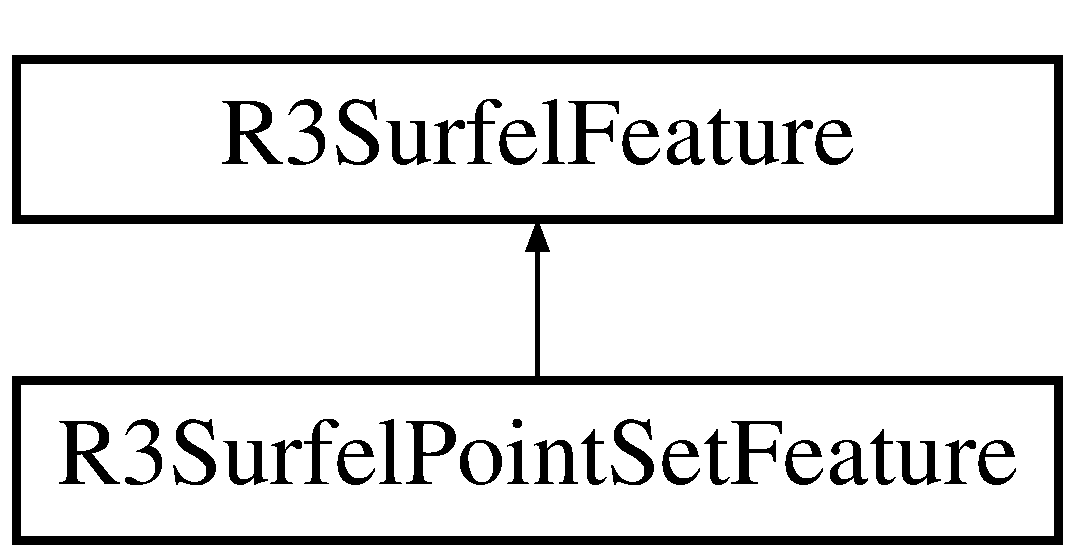
\includegraphics[height=2.000000cm]{class_r3_surfel_point_set_feature}
\end{center}
\end{figure}
\subsection*{Public Member Functions}
\begin{DoxyCompactItemize}
\item 
{\bfseries R3\+Surfel\+Point\+Set\+Feature} (const char $\ast$name=N\+U\+LL, R\+N\+Scalar minimum=-\/F\+L\+T\+\_\+\+M\+AX, R\+N\+Scalar maximum=F\+L\+T\+\_\+\+M\+AX, R\+N\+Scalar weight=1)\hypertarget{class_r3_surfel_point_set_feature_a60df541a802fa347dd86550fd08f2557}{}\label{class_r3_surfel_point_set_feature_a60df541a802fa347dd86550fd08f2557}

\item 
virtual int {\bfseries Type} (void) const \hypertarget{class_r3_surfel_point_set_feature_a888df9bb9dfaea2ece0210517b88a820}{}\label{class_r3_surfel_point_set_feature_a888df9bb9dfaea2ece0210517b88a820}

\item 
virtual int {\bfseries Update\+Feature\+Vector} (\hyperlink{class_r3_surfel_object}{R3\+Surfel\+Object} $\ast$object, \hyperlink{class_r3_surfel_feature_vector}{R3\+Surfel\+Feature\+Vector} \&vector) const \hypertarget{class_r3_surfel_point_set_feature_ac605bd460cc29497ac1790e93c6cbb98}{}\label{class_r3_surfel_point_set_feature_ac605bd460cc29497ac1790e93c6cbb98}

\end{DoxyCompactItemize}


The documentation for this class was generated from the following files\+:\begin{DoxyCompactItemize}
\item 
R3\+Surfels/R3\+Surfel\+Feature\+Evaluation.\+h\item 
R3\+Surfels/R3\+Surfel\+Feature\+Evaluation.\+cpp\end{DoxyCompactItemize}

\hypertarget{class_r3_surfel_scan}{}\section{R3\+Surfel\+Scan Class Reference}
\label{class_r3_surfel_scan}\index{R3\+Surfel\+Scan@{R3\+Surfel\+Scan}}
\subsection*{Public Member Functions}
\begin{DoxyCompactItemize}
\item 
{\bfseries R3\+Surfel\+Scan} (const char $\ast$name=N\+U\+LL)\hypertarget{class_r3_surfel_scan_a0b6693f3ad10b3e7b47e205d7fb5c655}{}\label{class_r3_surfel_scan_a0b6693f3ad10b3e7b47e205d7fb5c655}

\item 
{\bfseries R3\+Surfel\+Scan} (const \hyperlink{class_r3_surfel_scan}{R3\+Surfel\+Scan} \&scan)\hypertarget{class_r3_surfel_scan_a886b2b11f8f0d701f705a8b3e5b3a899}{}\label{class_r3_surfel_scan_a886b2b11f8f0d701f705a8b3e5b3a899}

\item 
int {\bfseries Width} (void) const \hypertarget{class_r3_surfel_scan_a1111c1a946869fd4fdc3f52cce43d319}{}\label{class_r3_surfel_scan_a1111c1a946869fd4fdc3f52cce43d319}

\item 
int {\bfseries Height} (void) const \hypertarget{class_r3_surfel_scan_ae1fa1489079a20d6e923f64c94288314}{}\label{class_r3_surfel_scan_ae1fa1489079a20d6e923f64c94288314}

\item 
const \hyperlink{class_r3_coord_system}{R3\+Coord\+System} \& {\bfseries Pose} (void) const \hypertarget{class_r3_surfel_scan_a5ecc0f26b6c9654b2b6f7da37afbcf4d}{}\label{class_r3_surfel_scan_a5ecc0f26b6c9654b2b6f7da37afbcf4d}

\item 
const \hyperlink{class_r3_point}{R3\+Point} \& {\bfseries Viewpoint} (void) const \hypertarget{class_r3_surfel_scan_a17383311bedbed659456376c3ddc4dcf}{}\label{class_r3_surfel_scan_a17383311bedbed659456376c3ddc4dcf}

\item 
\hyperlink{class_r3_vector}{R3\+Vector} {\bfseries Towards} (void) const \hypertarget{class_r3_surfel_scan_abbd8656de1be6460852e690bdd9155cb}{}\label{class_r3_surfel_scan_abbd8656de1be6460852e690bdd9155cb}

\item 
const \hyperlink{class_r3_vector}{R3\+Vector} \& {\bfseries Up} (void) const \hypertarget{class_r3_surfel_scan_aca583f253a8eb896894ea90397c48b6c}{}\label{class_r3_surfel_scan_aca583f253a8eb896894ea90397c48b6c}

\item 
const \hyperlink{class_r3_vector}{R3\+Vector} \& {\bfseries Right} (void) const \hypertarget{class_r3_surfel_scan_a39a4db91883084f22ac2834f8351c9b5}{}\label{class_r3_surfel_scan_a39a4db91883084f22ac2834f8351c9b5}

\item 
R\+N\+Angle {\bfseries Focal\+Length} (void) const \hypertarget{class_r3_surfel_scan_a9288c278db44df33c16aff17820b24ca}{}\label{class_r3_surfel_scan_a9288c278db44df33c16aff17820b24ca}

\item 
R\+N\+Angle {\bfseries X\+F\+OV} (void) const \hypertarget{class_r3_surfel_scan_a215bb1c27f548ae4edd1d68926d3284d}{}\label{class_r3_surfel_scan_a215bb1c27f548ae4edd1d68926d3284d}

\item 
R\+N\+Angle {\bfseries Y\+F\+OV} (void) const \hypertarget{class_r3_surfel_scan_a03e61a614e3d2da943321b6dd0e69530}{}\label{class_r3_surfel_scan_a03e61a614e3d2da943321b6dd0e69530}

\item 
const \hyperlink{class_r3_box}{R3\+Box} \& {\bfseries B\+Box} (void) const \hypertarget{class_r3_surfel_scan_a52c884c9f2fa6c44431abdde34a25054}{}\label{class_r3_surfel_scan_a52c884c9f2fa6c44431abdde34a25054}

\item 
\hyperlink{class_r3_point}{R3\+Point} {\bfseries Centroid} (void) const \hypertarget{class_r3_surfel_scan_aa51ec9a018912d9b47c0638bdcabff58}{}\label{class_r3_surfel_scan_aa51ec9a018912d9b47c0638bdcabff58}

\item 
R\+N\+Scalar {\bfseries Timestamp} (void) const \hypertarget{class_r3_surfel_scan_a7858b65d2f14fedd76869190bb154fae}{}\label{class_r3_surfel_scan_a7858b65d2f14fedd76869190bb154fae}

\item 
const char $\ast$ {\bfseries Name} (void) const \hypertarget{class_r3_surfel_scan_ae574131859894cb50b97ce61b877f95b}{}\label{class_r3_surfel_scan_ae574131859894cb50b97ce61b877f95b}

\item 
void $\ast$ {\bfseries Data} (void) const \hypertarget{class_r3_surfel_scan_a8d4d9ec9f860f249046143f33a9058e8}{}\label{class_r3_surfel_scan_a8d4d9ec9f860f249046143f33a9058e8}

\item 
\hyperlink{class_r3_surfel_scene}{R3\+Surfel\+Scene} $\ast$ {\bfseries Scene} (void) const \hypertarget{class_r3_surfel_scan_a188014b2ac5cccdc2616ce63e8578024}{}\label{class_r3_surfel_scan_a188014b2ac5cccdc2616ce63e8578024}

\item 
int {\bfseries Scene\+Index} (void) const \hypertarget{class_r3_surfel_scan_a88c6711e9e6ba048c0cad616cca3e2d1}{}\label{class_r3_surfel_scan_a88c6711e9e6ba048c0cad616cca3e2d1}

\item 
\hyperlink{class_r3_surfel_node}{R3\+Surfel\+Node} $\ast$ {\bfseries Node} (void) const \hypertarget{class_r3_surfel_scan_aeefba600143ba1580f8c5a2ba19af89e}{}\label{class_r3_surfel_scan_aeefba600143ba1580f8c5a2ba19af89e}

\item 
\hyperlink{class_r3_surfel_point_set}{R3\+Surfel\+Point\+Set} $\ast$ {\bfseries Point\+Set} (void) const \hypertarget{class_r3_surfel_scan_a9fbc0a5e5b2ddcf6efae9cce609e8d2b}{}\label{class_r3_surfel_scan_a9fbc0a5e5b2ddcf6efae9cce609e8d2b}

\item 
virtual void {\bfseries Set\+Pose} (const \hyperlink{class_r3_coord_system}{R3\+Coord\+System} \&pose)\hypertarget{class_r3_surfel_scan_ac19a0bd15a6512fa0b95be049e85d0be}{}\label{class_r3_surfel_scan_ac19a0bd15a6512fa0b95be049e85d0be}

\item 
virtual void {\bfseries Set\+Viewpoint} (const \hyperlink{class_r3_point}{R3\+Point} \&viewpoint)\hypertarget{class_r3_surfel_scan_ab2b55b8ed10befcf34fa9aa811387b80}{}\label{class_r3_surfel_scan_ab2b55b8ed10befcf34fa9aa811387b80}

\item 
virtual void {\bfseries Set\+Orientation} (const \hyperlink{class_r3_vector}{R3\+Vector} \&towards, const \hyperlink{class_r3_vector}{R3\+Vector} \&up)\hypertarget{class_r3_surfel_scan_a2ee699eba3be44785c3e5b2c24f082c1}{}\label{class_r3_surfel_scan_a2ee699eba3be44785c3e5b2c24f082c1}

\item 
virtual void {\bfseries Set\+Focal\+Length} (R\+N\+Length focal\+\_\+length)\hypertarget{class_r3_surfel_scan_ab38c49d41ed154ddf2a0a666b6fc2fd1}{}\label{class_r3_surfel_scan_ab38c49d41ed154ddf2a0a666b6fc2fd1}

\item 
virtual void {\bfseries Set\+Timestamp} (R\+N\+Scalar timestamp)\hypertarget{class_r3_surfel_scan_a9b911637cbfb2ff69f24819e0823bc66}{}\label{class_r3_surfel_scan_a9b911637cbfb2ff69f24819e0823bc66}

\item 
virtual void {\bfseries Set\+Name} (const char $\ast$name)\hypertarget{class_r3_surfel_scan_a42e40bd5fd81612c9f8a979fb02c98e9}{}\label{class_r3_surfel_scan_a42e40bd5fd81612c9f8a979fb02c98e9}

\item 
virtual void {\bfseries Set\+Data} (void $\ast$data)\hypertarget{class_r3_surfel_scan_af3bbf1d1a584acf9043e885e7c2d92f4}{}\label{class_r3_surfel_scan_af3bbf1d1a584acf9043e885e7c2d92f4}

\item 
virtual void {\bfseries Set\+Resolution} (int width, int height)\hypertarget{class_r3_surfel_scan_a4847caa724ecd12dcbd37909552a40bb}{}\label{class_r3_surfel_scan_a4847caa724ecd12dcbd37909552a40bb}

\item 
virtual void {\bfseries Set\+Node} (\hyperlink{class_r3_surfel_node}{R3\+Surfel\+Node} $\ast$node)\hypertarget{class_r3_surfel_scan_a7750612aeb9adc276893113ae3f18c52}{}\label{class_r3_surfel_scan_a7750612aeb9adc276893113ae3f18c52}

\item 
void {\bfseries Read\+Blocks} (void)\hypertarget{class_r3_surfel_scan_a3bed3552a4e40ed660c3c1250cecbe21}{}\label{class_r3_surfel_scan_a3bed3552a4e40ed660c3c1250cecbe21}

\item 
void {\bfseries Release\+Blocks} (void)\hypertarget{class_r3_surfel_scan_a39d6498c4eefe56cc69909f6185af692}{}\label{class_r3_surfel_scan_a39d6498c4eefe56cc69909f6185af692}

\item 
R\+N\+Boolean {\bfseries Are\+Blocks\+Resident} (void) const \hypertarget{class_r3_surfel_scan_a1200bc3c902ff266860781c8c316be69}{}\label{class_r3_surfel_scan_a1200bc3c902ff266860781c8c316be69}

\item 
virtual void {\bfseries Draw} (\hyperlink{class_r_n_flags}{R\+N\+Flags} flags=R3\+\_\+\+S\+U\+R\+F\+E\+L\+\_\+\+D\+E\+F\+A\+U\+L\+T\+\_\+\+D\+R\+A\+W\+\_\+\+F\+L\+A\+GS) const \hypertarget{class_r3_surfel_scan_a3967df9732b70165ec7936c62369353b}{}\label{class_r3_surfel_scan_a3967df9732b70165ec7936c62369353b}

\item 
virtual void {\bfseries Print} (F\+I\+LE $\ast$fp=N\+U\+LL, const char $\ast$prefix=N\+U\+LL, const char $\ast$suffix=N\+U\+LL) const \hypertarget{class_r3_surfel_scan_ac0dae36e5d8ce1bc7d174f878e0bf712}{}\label{class_r3_surfel_scan_ac0dae36e5d8ce1bc7d174f878e0bf712}

\end{DoxyCompactItemize}
\subsection*{Protected Attributes}
\begin{DoxyCompactItemize}
\item 
\hyperlink{class_r3_surfel_scene}{R3\+Surfel\+Scene} $\ast$ {\bfseries scene}\hypertarget{class_r3_surfel_scan_a7b8401558d53080b02d43e40cf3c2445}{}\label{class_r3_surfel_scan_a7b8401558d53080b02d43e40cf3c2445}

\item 
int {\bfseries scene\+\_\+index}\hypertarget{class_r3_surfel_scan_ac16755aae933fa898f34d7ef6c49ae14}{}\label{class_r3_surfel_scan_ac16755aae933fa898f34d7ef6c49ae14}

\item 
\hyperlink{class_r3_surfel_node}{R3\+Surfel\+Node} $\ast$ {\bfseries node}\hypertarget{class_r3_surfel_scan_a182dfddf15c0ce47545a396284f0da9f}{}\label{class_r3_surfel_scan_a182dfddf15c0ce47545a396284f0da9f}

\item 
\hyperlink{class_r3_coord_system}{R3\+Coord\+System} {\bfseries pose}\hypertarget{class_r3_surfel_scan_a2f228142083d4afd913232f9cb671ef9}{}\label{class_r3_surfel_scan_a2f228142083d4afd913232f9cb671ef9}

\item 
R\+N\+Length {\bfseries focal\+\_\+length}\hypertarget{class_r3_surfel_scan_a0389a055a0ae263a8324060dc33a2491}{}\label{class_r3_surfel_scan_a0389a055a0ae263a8324060dc33a2491}

\item 
R\+N\+Scalar {\bfseries timestamp}\hypertarget{class_r3_surfel_scan_af88736e404e1ebe8345f4407b55ad3e0}{}\label{class_r3_surfel_scan_af88736e404e1ebe8345f4407b55ad3e0}

\item 
int {\bfseries width}\hypertarget{class_r3_surfel_scan_ae4f4197885ef489184acad27b576841d}{}\label{class_r3_surfel_scan_ae4f4197885ef489184acad27b576841d}

\item 
int {\bfseries height}\hypertarget{class_r3_surfel_scan_af4d956b166dc8a6fd60d0624f46e5d13}{}\label{class_r3_surfel_scan_af4d956b166dc8a6fd60d0624f46e5d13}

\item 
char $\ast$ {\bfseries name}\hypertarget{class_r3_surfel_scan_a6f10bc0db5d2f89f1c909fbf521eb096}{}\label{class_r3_surfel_scan_a6f10bc0db5d2f89f1c909fbf521eb096}

\item 
\hyperlink{class_r_n_flags}{R\+N\+Flags} {\bfseries flags}\hypertarget{class_r3_surfel_scan_a8ac96d3b751adb5d81a6dfe2fa5d0d7f}{}\label{class_r3_surfel_scan_a8ac96d3b751adb5d81a6dfe2fa5d0d7f}

\item 
void $\ast$ {\bfseries data}\hypertarget{class_r3_surfel_scan_a7e36bf1fa79831b6c1784c2d1c76d509}{}\label{class_r3_surfel_scan_a7e36bf1fa79831b6c1784c2d1c76d509}

\end{DoxyCompactItemize}
\subsection*{Friends}
\begin{DoxyCompactItemize}
\item 
class {\bfseries R3\+Surfel\+Scene}\hypertarget{class_r3_surfel_scan_af9bb32c0eac7d1d54787bbc6b44586b6}{}\label{class_r3_surfel_scan_af9bb32c0eac7d1d54787bbc6b44586b6}

\end{DoxyCompactItemize}


The documentation for this class was generated from the following files\+:\begin{DoxyCompactItemize}
\item 
R3\+Surfels/R3\+Surfel\+Scan.\+h\item 
R3\+Surfels/R3\+Surfel\+Scan.\+cpp\end{DoxyCompactItemize}

\hypertarget{class_r3_surfel_scene}{}\section{R3\+Surfel\+Scene Class Reference}
\label{class_r3_surfel_scene}\index{R3\+Surfel\+Scene@{R3\+Surfel\+Scene}}
\subsection*{Public Member Functions}
\begin{DoxyCompactItemize}
\item 
{\bfseries R3\+Surfel\+Scene} (const char $\ast$name=N\+U\+LL)\hypertarget{class_r3_surfel_scene_a71cdf9f385093b44b2c3a752dd03eff1}{}\label{class_r3_surfel_scene_a71cdf9f385093b44b2c3a752dd03eff1}

\item 
{\bfseries R3\+Surfel\+Scene} (const \hyperlink{class_r3_surfel_scene}{R3\+Surfel\+Scene} \&scene)\hypertarget{class_r3_surfel_scene_a8f501256ddf0b017856d8916af9d0bcb}{}\label{class_r3_surfel_scene_a8f501256ddf0b017856d8916af9d0bcb}

\item 
const \hyperlink{class_r3_box}{R3\+Box} \& {\bfseries B\+Box} (void) const \hypertarget{class_r3_surfel_scene_aef52657a0cec8dbfd37fb4bb65a5a875}{}\label{class_r3_surfel_scene_aef52657a0cec8dbfd37fb4bb65a5a875}

\item 
\hyperlink{class_r3_point}{R3\+Point} {\bfseries Centroid} (void) const \hypertarget{class_r3_surfel_scene_a4047a286060f1531cd56978ff865f005}{}\label{class_r3_surfel_scene_a4047a286060f1531cd56978ff865f005}

\item 
const char $\ast$ {\bfseries Name} (void) const \hypertarget{class_r3_surfel_scene_ad9a826a9b2065410935a9834ea9b1639}{}\label{class_r3_surfel_scene_ad9a826a9b2065410935a9834ea9b1639}

\item 
\hyperlink{class_r3_surfel_tree}{R3\+Surfel\+Tree} $\ast$ {\bfseries Tree} (void) const \hypertarget{class_r3_surfel_scene_abfac6b3ecb73acacf331f03e9ae87102}{}\label{class_r3_surfel_scene_abfac6b3ecb73acacf331f03e9ae87102}

\item 
int {\bfseries N\+Objects} (void) const \hypertarget{class_r3_surfel_scene_a8acfa61b6a7c69ee48906d19d5d57159}{}\label{class_r3_surfel_scene_a8acfa61b6a7c69ee48906d19d5d57159}

\item 
\hyperlink{class_r3_surfel_object}{R3\+Surfel\+Object} $\ast$ {\bfseries Object} (int k) const \hypertarget{class_r3_surfel_scene_a0930c85684b8991f6ea996cf6f94b21c}{}\label{class_r3_surfel_scene_a0930c85684b8991f6ea996cf6f94b21c}

\item 
\hyperlink{class_r3_surfel_object}{R3\+Surfel\+Object} $\ast$ {\bfseries Find\+Object\+By\+Name} (const char $\ast$object\+\_\+name) const \hypertarget{class_r3_surfel_scene_a2d4fa33fd2990bdd2a2fc9f0100aa470}{}\label{class_r3_surfel_scene_a2d4fa33fd2990bdd2a2fc9f0100aa470}

\item 
\hyperlink{class_r3_surfel_object}{R3\+Surfel\+Object} $\ast$ {\bfseries Find\+Object\+By\+Identifier} (int identifier) const \hypertarget{class_r3_surfel_scene_acd2d381711eed1f1f23a9ef4f34f1549}{}\label{class_r3_surfel_scene_acd2d381711eed1f1f23a9ef4f34f1549}

\item 
\hyperlink{class_r3_surfel_object}{R3\+Surfel\+Object} $\ast$ {\bfseries Root\+Object} (void) const \hypertarget{class_r3_surfel_scene_a26ef482636666568bbaf6d70df9f0de1}{}\label{class_r3_surfel_scene_a26ef482636666568bbaf6d70df9f0de1}

\item 
int {\bfseries N\+Labels} (void) const \hypertarget{class_r3_surfel_scene_a1e9aa48a490fa9d5c821ca84c0fb192e}{}\label{class_r3_surfel_scene_a1e9aa48a490fa9d5c821ca84c0fb192e}

\item 
\hyperlink{class_r3_surfel_label}{R3\+Surfel\+Label} $\ast$ {\bfseries Label} (int k) const \hypertarget{class_r3_surfel_scene_a6678d7cd3a1f3995efb4ad5a8beff973}{}\label{class_r3_surfel_scene_a6678d7cd3a1f3995efb4ad5a8beff973}

\item 
\hyperlink{class_r3_surfel_label}{R3\+Surfel\+Label} $\ast$ {\bfseries Find\+Label\+By\+Name} (const char $\ast$label\+\_\+name) const \hypertarget{class_r3_surfel_scene_a778ea8f52e821415d76e94dfe87835dd}{}\label{class_r3_surfel_scene_a778ea8f52e821415d76e94dfe87835dd}

\item 
\hyperlink{class_r3_surfel_label}{R3\+Surfel\+Label} $\ast$ {\bfseries Find\+Label\+By\+Identifier} (int identifier) const \hypertarget{class_r3_surfel_scene_aa8257233ef030f9a9b859c91ac9dcd4a}{}\label{class_r3_surfel_scene_aa8257233ef030f9a9b859c91ac9dcd4a}

\item 
\hyperlink{class_r3_surfel_label}{R3\+Surfel\+Label} $\ast$ {\bfseries Find\+Label\+By\+Assignment\+Keystroke} (int key) const \hypertarget{class_r3_surfel_scene_ab3528dd8cd14f89d0a1e28c0a28233d8}{}\label{class_r3_surfel_scene_ab3528dd8cd14f89d0a1e28c0a28233d8}

\item 
\hyperlink{class_r3_surfel_label}{R3\+Surfel\+Label} $\ast$ {\bfseries Root\+Label} (void) const \hypertarget{class_r3_surfel_scene_ad977eb03cd0721a2824f1e8d3b7e21c3}{}\label{class_r3_surfel_scene_ad977eb03cd0721a2824f1e8d3b7e21c3}

\item 
int {\bfseries N\+Object\+Properties} (void) const \hypertarget{class_r3_surfel_scene_aee63940c67184c7dbde0ed831745abe3}{}\label{class_r3_surfel_scene_aee63940c67184c7dbde0ed831745abe3}

\item 
\hyperlink{class_r3_surfel_object_property}{R3\+Surfel\+Object\+Property} $\ast$ {\bfseries Object\+Property} (int k) const \hypertarget{class_r3_surfel_scene_a990f21e9470403781aeccace1a1a38ff}{}\label{class_r3_surfel_scene_a990f21e9470403781aeccace1a1a38ff}

\item 
int {\bfseries N\+Label\+Properties} (void) const \hypertarget{class_r3_surfel_scene_ad511d5aebf6424385407e9e3c7fb8ee5}{}\label{class_r3_surfel_scene_ad511d5aebf6424385407e9e3c7fb8ee5}

\item 
\hyperlink{class_r3_surfel_label_property}{R3\+Surfel\+Label\+Property} $\ast$ {\bfseries Label\+Property} (int k) const \hypertarget{class_r3_surfel_scene_aedc1efc6daa22f59ae7e8d74bc506cf5}{}\label{class_r3_surfel_scene_aedc1efc6daa22f59ae7e8d74bc506cf5}

\item 
int {\bfseries N\+Object\+Relationships} (void) const \hypertarget{class_r3_surfel_scene_ae242fd487ff6b51034f564197556def2}{}\label{class_r3_surfel_scene_ae242fd487ff6b51034f564197556def2}

\item 
\hyperlink{class_r3_surfel_object_relationship}{R3\+Surfel\+Object\+Relationship} $\ast$ {\bfseries Object\+Relationship} (int k) const \hypertarget{class_r3_surfel_scene_a16e49e0502eef548480b24095d0773d6}{}\label{class_r3_surfel_scene_a16e49e0502eef548480b24095d0773d6}

\item 
int {\bfseries N\+Label\+Relationships} (void) const \hypertarget{class_r3_surfel_scene_aad4cc50e0264b50fcf9d23ed218a5fd0}{}\label{class_r3_surfel_scene_aad4cc50e0264b50fcf9d23ed218a5fd0}

\item 
\hyperlink{class_r3_surfel_label_relationship}{R3\+Surfel\+Label\+Relationship} $\ast$ {\bfseries Label\+Relationship} (int k) const \hypertarget{class_r3_surfel_scene_abe517227057122990ce0f5d1d3d9fc43}{}\label{class_r3_surfel_scene_abe517227057122990ce0f5d1d3d9fc43}

\item 
int {\bfseries N\+Label\+Assignments} (void) const \hypertarget{class_r3_surfel_scene_aaff3a67de215e280c8bf1942ba714447}{}\label{class_r3_surfel_scene_aaff3a67de215e280c8bf1942ba714447}

\item 
\hyperlink{class_r3_surfel_label_assignment}{R3\+Surfel\+Label\+Assignment} $\ast$ {\bfseries Label\+Assignment} (int k) const \hypertarget{class_r3_surfel_scene_aa428129f83c1d499154aa751de035a7a}{}\label{class_r3_surfel_scene_aa428129f83c1d499154aa751de035a7a}

\item 
\hyperlink{class_r3_surfel_label_assignment}{R3\+Surfel\+Label\+Assignment} $\ast$ {\bfseries Find\+Label\+Assignment} (\hyperlink{class_r3_surfel_object}{R3\+Surfel\+Object} $\ast$object, \hyperlink{class_r3_surfel_label}{R3\+Surfel\+Label} $\ast$label, R\+N\+Scalar confidence, int originator) const \hypertarget{class_r3_surfel_scene_ab2f00b2ce4c676dce0f02a51f56ba83e}{}\label{class_r3_surfel_scene_ab2f00b2ce4c676dce0f02a51f56ba83e}

\item 
int {\bfseries N\+Scans} (void) const \hypertarget{class_r3_surfel_scene_ab9bd6ca17f3f64f94c722307781029fe}{}\label{class_r3_surfel_scene_ab9bd6ca17f3f64f94c722307781029fe}

\item 
\hyperlink{class_r3_surfel_scan}{R3\+Surfel\+Scan} $\ast$ {\bfseries Scan} (int k) const \hypertarget{class_r3_surfel_scene_a318c042f99619aaea18fd1d422ba1dac}{}\label{class_r3_surfel_scene_a318c042f99619aaea18fd1d422ba1dac}

\item 
\hyperlink{class_r3_surfel_scan}{R3\+Surfel\+Scan} $\ast$ {\bfseries Find\+Scan\+By\+Name} (const char $\ast$scan\+\_\+name) const \hypertarget{class_r3_surfel_scene_ae00d75c742b1ff423b5205c75c206681}{}\label{class_r3_surfel_scene_ae00d75c742b1ff423b5205c75c206681}

\item 
int {\bfseries N\+Features} (void) const \hypertarget{class_r3_surfel_scene_a974946cd84eefd3b93487104b89806a7}{}\label{class_r3_surfel_scene_a974946cd84eefd3b93487104b89806a7}

\item 
\hyperlink{class_r3_surfel_feature}{R3\+Surfel\+Feature} $\ast$ {\bfseries Feature} (int k) const \hypertarget{class_r3_surfel_scene_aa791b22ec9717bdea2dce94017d1c299}{}\label{class_r3_surfel_scene_aa791b22ec9717bdea2dce94017d1c299}

\item 
\hyperlink{class_r3_surfel_feature}{R3\+Surfel\+Feature} $\ast$ {\bfseries Find\+Feature\+By\+Name} (const char $\ast$feature\+\_\+name) const \hypertarget{class_r3_surfel_scene_a4c9ac9086beaece12a51dc4d764db3d5}{}\label{class_r3_surfel_scene_a4c9ac9086beaece12a51dc4d764db3d5}

\item 
virtual void {\bfseries Set\+Name} (const char $\ast$name)\hypertarget{class_r3_surfel_scene_ab1597ca57353375b0192657bed019ee7}{}\label{class_r3_surfel_scene_ab1597ca57353375b0192657bed019ee7}

\item 
virtual void {\bfseries Insert\+Object} (\hyperlink{class_r3_surfel_object}{R3\+Surfel\+Object} $\ast$object, \hyperlink{class_r3_surfel_object}{R3\+Surfel\+Object} $\ast$parent)\hypertarget{class_r3_surfel_scene_a297d021200f2187c2bf56770fa9961f4}{}\label{class_r3_surfel_scene_a297d021200f2187c2bf56770fa9961f4}

\item 
virtual void {\bfseries Remove\+Object} (\hyperlink{class_r3_surfel_object}{R3\+Surfel\+Object} $\ast$object)\hypertarget{class_r3_surfel_scene_ae2d77aefc703271af5ef294346d2a489}{}\label{class_r3_surfel_scene_ae2d77aefc703271af5ef294346d2a489}

\item 
virtual void {\bfseries Merge\+Object} (\hyperlink{class_r3_surfel_object}{R3\+Surfel\+Object} $\ast$dst\+\_\+object, \hyperlink{class_r3_surfel_object}{R3\+Surfel\+Object} $\ast$src\+\_\+object)\hypertarget{class_r3_surfel_scene_a2b7156bc0316f89246c20b95bff478b3}{}\label{class_r3_surfel_scene_a2b7156bc0316f89246c20b95bff478b3}

\item 
virtual void {\bfseries Insert\+Label} (\hyperlink{class_r3_surfel_label}{R3\+Surfel\+Label} $\ast$label, \hyperlink{class_r3_surfel_label}{R3\+Surfel\+Label} $\ast$parent)\hypertarget{class_r3_surfel_scene_aa7edafa9893be74dc43b319121ebefeb}{}\label{class_r3_surfel_scene_aa7edafa9893be74dc43b319121ebefeb}

\item 
virtual void {\bfseries Remove\+Label} (\hyperlink{class_r3_surfel_label}{R3\+Surfel\+Label} $\ast$label)\hypertarget{class_r3_surfel_scene_af1660e17332532370fba91b27da37588}{}\label{class_r3_surfel_scene_af1660e17332532370fba91b27da37588}

\item 
virtual void {\bfseries Insert\+Object\+Property} (\hyperlink{class_r3_surfel_object_property}{R3\+Surfel\+Object\+Property} $\ast$property)\hypertarget{class_r3_surfel_scene_ad9928a09633e9bf0542dc4e76748d4a0}{}\label{class_r3_surfel_scene_ad9928a09633e9bf0542dc4e76748d4a0}

\item 
virtual void {\bfseries Remove\+Object\+Property} (\hyperlink{class_r3_surfel_object_property}{R3\+Surfel\+Object\+Property} $\ast$property)\hypertarget{class_r3_surfel_scene_a8e370f15e72ed99f00a5339f3c919bf5}{}\label{class_r3_surfel_scene_a8e370f15e72ed99f00a5339f3c919bf5}

\item 
virtual void {\bfseries Insert\+Label\+Property} (\hyperlink{class_r3_surfel_label_property}{R3\+Surfel\+Label\+Property} $\ast$property)\hypertarget{class_r3_surfel_scene_a6e4df173fe79288bc50dc832fc5b416f}{}\label{class_r3_surfel_scene_a6e4df173fe79288bc50dc832fc5b416f}

\item 
virtual void {\bfseries Remove\+Label\+Property} (\hyperlink{class_r3_surfel_label_property}{R3\+Surfel\+Label\+Property} $\ast$property)\hypertarget{class_r3_surfel_scene_aac214ba3ffa72a973190a9491a397cb4}{}\label{class_r3_surfel_scene_aac214ba3ffa72a973190a9491a397cb4}

\item 
virtual void {\bfseries Insert\+Object\+Relationship} (\hyperlink{class_r3_surfel_object_relationship}{R3\+Surfel\+Object\+Relationship} $\ast$relationship)\hypertarget{class_r3_surfel_scene_a40a5c1783624fad870c599bd41f1ced2}{}\label{class_r3_surfel_scene_a40a5c1783624fad870c599bd41f1ced2}

\item 
virtual void {\bfseries Remove\+Object\+Relationship} (\hyperlink{class_r3_surfel_object_relationship}{R3\+Surfel\+Object\+Relationship} $\ast$relationship)\hypertarget{class_r3_surfel_scene_a948b3d04d3218963d35de3e61315dd44}{}\label{class_r3_surfel_scene_a948b3d04d3218963d35de3e61315dd44}

\item 
virtual void {\bfseries Insert\+Label\+Relationship} (\hyperlink{class_r3_surfel_label_relationship}{R3\+Surfel\+Label\+Relationship} $\ast$relationship)\hypertarget{class_r3_surfel_scene_a4fe2f7dafecbc074bc649a4650b1476d}{}\label{class_r3_surfel_scene_a4fe2f7dafecbc074bc649a4650b1476d}

\item 
virtual void {\bfseries Remove\+Label\+Relationship} (\hyperlink{class_r3_surfel_label_relationship}{R3\+Surfel\+Label\+Relationship} $\ast$relationship)\hypertarget{class_r3_surfel_scene_a99be6c1d7776aca09d59d041d73cb6e3}{}\label{class_r3_surfel_scene_a99be6c1d7776aca09d59d041d73cb6e3}

\item 
virtual void {\bfseries Insert\+Label\+Assignment} (\hyperlink{class_r3_surfel_label_assignment}{R3\+Surfel\+Label\+Assignment} $\ast$assignment)\hypertarget{class_r3_surfel_scene_aeca672ddfce30f9f49e957794dc55a57}{}\label{class_r3_surfel_scene_aeca672ddfce30f9f49e957794dc55a57}

\item 
virtual void {\bfseries Remove\+Label\+Assignment} (\hyperlink{class_r3_surfel_label_assignment}{R3\+Surfel\+Label\+Assignment} $\ast$assignment)\hypertarget{class_r3_surfel_scene_ab0e26b98501b18016e2bf5f1f799984a}{}\label{class_r3_surfel_scene_ab0e26b98501b18016e2bf5f1f799984a}

\item 
virtual void {\bfseries Insert\+Scan} (\hyperlink{class_r3_surfel_scan}{R3\+Surfel\+Scan} $\ast$scan)\hypertarget{class_r3_surfel_scene_a46ede81772f690d39f3e742e7ccfb8d4}{}\label{class_r3_surfel_scene_a46ede81772f690d39f3e742e7ccfb8d4}

\item 
virtual void {\bfseries Remove\+Scan} (\hyperlink{class_r3_surfel_scan}{R3\+Surfel\+Scan} $\ast$scan)\hypertarget{class_r3_surfel_scene_a9a11318e18837dd55bfb0e1f9e8fd340}{}\label{class_r3_surfel_scene_a9a11318e18837dd55bfb0e1f9e8fd340}

\item 
virtual void {\bfseries Insert\+Feature} (\hyperlink{class_r3_surfel_feature}{R3\+Surfel\+Feature} $\ast$feature)\hypertarget{class_r3_surfel_scene_a0536a7acda168fe260bcc899dd55bf90}{}\label{class_r3_surfel_scene_a0536a7acda168fe260bcc899dd55bf90}

\item 
virtual void {\bfseries Remove\+Feature} (\hyperlink{class_r3_surfel_feature}{R3\+Surfel\+Feature} $\ast$feature)\hypertarget{class_r3_surfel_scene_a65e9684c631df43dfef3d7e12f83fb1f}{}\label{class_r3_surfel_scene_a65e9684c631df43dfef3d7e12f83fb1f}

\item 
virtual void {\bfseries Insert\+Scene} (const \hyperlink{class_r3_surfel_scene}{R3\+Surfel\+Scene} \&scene2, \hyperlink{class_r3_surfel_object}{R3\+Surfel\+Object} $\ast$parent\+\_\+object1=N\+U\+LL, \hyperlink{class_r3_surfel_label}{R3\+Surfel\+Label} $\ast$parent\+\_\+label1=N\+U\+LL, \hyperlink{class_r3_surfel_node}{R3\+Surfel\+Node} $\ast$parent\+\_\+node1=N\+U\+LL)\hypertarget{class_r3_surfel_scene_ac71b934287f70616a51ab6e89e1cb05b}{}\label{class_r3_surfel_scene_ac71b934287f70616a51ab6e89e1cb05b}

\item 
virtual void {\bfseries Draw} (\hyperlink{class_r_n_flags}{R\+N\+Flags} flags=R3\+\_\+\+S\+U\+R\+F\+E\+L\+\_\+\+D\+E\+F\+A\+U\+L\+T\+\_\+\+D\+R\+A\+W\+\_\+\+F\+L\+A\+GS) const \hypertarget{class_r3_surfel_scene_a39a2895331a757858c28331533706f17}{}\label{class_r3_surfel_scene_a39a2895331a757858c28331533706f17}

\item 
virtual void {\bfseries Print} (F\+I\+LE $\ast$fp=N\+U\+LL, const char $\ast$prefix=N\+U\+LL, const char $\ast$suffix=N\+U\+LL) const \hypertarget{class_r3_surfel_scene_a0e6e2dc2ecb2811478aba53316564461}{}\label{class_r3_surfel_scene_a0e6e2dc2ecb2811478aba53316564461}

\item 
virtual int {\bfseries Open\+File} (const char $\ast$scene\+\_\+filename, const char $\ast$database\+\_\+filename, const char $\ast$scene\+\_\+rwaccess=N\+U\+LL, const char $\ast$database\+\_\+rwaccess=N\+U\+LL)\hypertarget{class_r3_surfel_scene_a1f4c23c978414e90f8ebbe42e09f4b4b}{}\label{class_r3_surfel_scene_a1f4c23c978414e90f8ebbe42e09f4b4b}

\item 
virtual int {\bfseries Sync\+File} (const char $\ast$output\+\_\+scene\+\_\+filename=N\+U\+LL)\hypertarget{class_r3_surfel_scene_a83d49ef4d3d30010d5cc88592cbb0dfc}{}\label{class_r3_surfel_scene_a83d49ef4d3d30010d5cc88592cbb0dfc}

\item 
virtual int {\bfseries Close\+File} (const char $\ast$output\+\_\+scene\+\_\+filename=N\+U\+LL)\hypertarget{class_r3_surfel_scene_a4e957a6b426d4df7951530603df522ab}{}\label{class_r3_surfel_scene_a4e957a6b426d4df7951530603df522ab}

\item 
void {\bfseries Set\+Dirty} (void)\hypertarget{class_r3_surfel_scene_ad75ada6bbd858db7d5ccf20aad03a81d}{}\label{class_r3_surfel_scene_ad75ada6bbd858db7d5ccf20aad03a81d}

\item 
virtual int {\bfseries Read\+File} (const char $\ast$filename)\hypertarget{class_r3_surfel_scene_aa1127051cc30232008abbcf48875b02d}{}\label{class_r3_surfel_scene_aa1127051cc30232008abbcf48875b02d}

\item 
virtual int {\bfseries Write\+File} (const char $\ast$filename)\hypertarget{class_r3_surfel_scene_af7b22843de09de955b57d7724a30ec4a}{}\label{class_r3_surfel_scene_af7b22843de09de955b57d7724a30ec4a}

\item 
virtual int {\bfseries Read\+Ascii\+File} (const char $\ast$filename)\hypertarget{class_r3_surfel_scene_a9ff325f3bb719086d6aca932deb49050}{}\label{class_r3_surfel_scene_a9ff325f3bb719086d6aca932deb49050}

\item 
virtual int {\bfseries Write\+Ascii\+File} (const char $\ast$filename)\hypertarget{class_r3_surfel_scene_a6aad289aab9336869de6d6066e326d59}{}\label{class_r3_surfel_scene_a6aad289aab9336869de6d6066e326d59}

\item 
virtual int {\bfseries Read\+Binary\+File} (const char $\ast$filename)\hypertarget{class_r3_surfel_scene_ae8ee21b1a55439d5543d189dea690252}{}\label{class_r3_surfel_scene_ae8ee21b1a55439d5543d189dea690252}

\item 
virtual int {\bfseries Write\+Binary\+File} (const char $\ast$filename)\hypertarget{class_r3_surfel_scene_a3a1489b58764a36a1445ef8171a6664e}{}\label{class_r3_surfel_scene_a3a1489b58764a36a1445ef8171a6664e}

\item 
virtual int {\bfseries Write\+A\+R\+F\+F\+File} (const char $\ast$filename)\hypertarget{class_r3_surfel_scene_a7487304e8c462560e822a247051a9bdb}{}\label{class_r3_surfel_scene_a7487304e8c462560e822a247051a9bdb}

\item 
virtual int {\bfseries Write\+Tianqiang\+File} (const char $\ast$filename)\hypertarget{class_r3_surfel_scene_a50e26f0ec234ae3794c23ce114b4b660}{}\label{class_r3_surfel_scene_a50e26f0ec234ae3794c23ce114b4b660}

\end{DoxyCompactItemize}
\subsection*{Protected Attributes}
\begin{DoxyCompactItemize}
\item 
\hyperlink{class_r3_surfel_tree}{R3\+Surfel\+Tree} $\ast$ {\bfseries tree}\hypertarget{class_r3_surfel_scene_a12f525d6f1d75f851047f4745430c07d}{}\label{class_r3_surfel_scene_a12f525d6f1d75f851047f4745430c07d}

\item 
\hyperlink{class_r_n_array}{R\+N\+Array}$<$ \hyperlink{class_r3_surfel_object}{R3\+Surfel\+Object} $\ast$ $>$ {\bfseries objects}\hypertarget{class_r3_surfel_scene_a5ce910401977268e9a158de57b0bd7e5}{}\label{class_r3_surfel_scene_a5ce910401977268e9a158de57b0bd7e5}

\item 
\hyperlink{class_r_n_array}{R\+N\+Array}$<$ \hyperlink{class_r3_surfel_label}{R3\+Surfel\+Label} $\ast$ $>$ {\bfseries labels}\hypertarget{class_r3_surfel_scene_a441745712132cae892b754aa37f69b22}{}\label{class_r3_surfel_scene_a441745712132cae892b754aa37f69b22}

\item 
\hyperlink{class_r_n_array}{R\+N\+Array}$<$ \hyperlink{class_r3_surfel_object_property}{R3\+Surfel\+Object\+Property} $\ast$ $>$ {\bfseries object\+\_\+properties}\hypertarget{class_r3_surfel_scene_a1d1941dc05573aaa55f981df166fb58f}{}\label{class_r3_surfel_scene_a1d1941dc05573aaa55f981df166fb58f}

\item 
\hyperlink{class_r_n_array}{R\+N\+Array}$<$ \hyperlink{class_r3_surfel_label_property}{R3\+Surfel\+Label\+Property} $\ast$ $>$ {\bfseries label\+\_\+properties}\hypertarget{class_r3_surfel_scene_a6708627dad0a6dd9955ba4d06e1b29b1}{}\label{class_r3_surfel_scene_a6708627dad0a6dd9955ba4d06e1b29b1}

\item 
\hyperlink{class_r_n_array}{R\+N\+Array}$<$ \hyperlink{class_r3_surfel_object_relationship}{R3\+Surfel\+Object\+Relationship} $\ast$ $>$ {\bfseries object\+\_\+relationships}\hypertarget{class_r3_surfel_scene_ad07e74ec2b6e60481b87ba0526d267e2}{}\label{class_r3_surfel_scene_ad07e74ec2b6e60481b87ba0526d267e2}

\item 
\hyperlink{class_r_n_array}{R\+N\+Array}$<$ \hyperlink{class_r3_surfel_label_relationship}{R3\+Surfel\+Label\+Relationship} $\ast$ $>$ {\bfseries label\+\_\+relationships}\hypertarget{class_r3_surfel_scene_a447d26a73919a335f815f65084c5143b}{}\label{class_r3_surfel_scene_a447d26a73919a335f815f65084c5143b}

\item 
\hyperlink{class_r_n_array}{R\+N\+Array}$<$ \hyperlink{class_r3_surfel_label_assignment}{R3\+Surfel\+Label\+Assignment} $\ast$ $>$ {\bfseries assignments}\hypertarget{class_r3_surfel_scene_a87c3608417a9381fd4cae245b878f25d}{}\label{class_r3_surfel_scene_a87c3608417a9381fd4cae245b878f25d}

\item 
\hyperlink{class_r_n_array}{R\+N\+Array}$<$ \hyperlink{class_r3_surfel_scan}{R3\+Surfel\+Scan} $\ast$ $>$ {\bfseries scans}\hypertarget{class_r3_surfel_scene_a17d62b9224b04f92428c8935f7904666}{}\label{class_r3_surfel_scene_a17d62b9224b04f92428c8935f7904666}

\item 
\hyperlink{class_r_n_array}{R\+N\+Array}$<$ \hyperlink{class_r3_surfel_feature}{R3\+Surfel\+Feature} $\ast$ $>$ {\bfseries features}\hypertarget{class_r3_surfel_scene_a85c19d4648e09d32568e35ed88d37f1b}{}\label{class_r3_surfel_scene_a85c19d4648e09d32568e35ed88d37f1b}

\item 
char $\ast$ {\bfseries filename}\hypertarget{class_r3_surfel_scene_ae85c94d0ff079c74599701a96ddeb4da}{}\label{class_r3_surfel_scene_ae85c94d0ff079c74599701a96ddeb4da}

\item 
char $\ast$ {\bfseries rwaccess}\hypertarget{class_r3_surfel_scene_a97987af0f79351237dd3211a0ac6a45d}{}\label{class_r3_surfel_scene_a97987af0f79351237dd3211a0ac6a45d}

\item 
char $\ast$ {\bfseries name}\hypertarget{class_r3_surfel_scene_a90d9969bbc2778a9aa2bc25dc792a757}{}\label{class_r3_surfel_scene_a90d9969bbc2778a9aa2bc25dc792a757}

\item 
\hyperlink{class_r_n_flags}{R\+N\+Flags} {\bfseries flags}\hypertarget{class_r3_surfel_scene_af94ebe6da866df3af411ad39f8bfb46a}{}\label{class_r3_surfel_scene_af94ebe6da866df3af411ad39f8bfb46a}

\end{DoxyCompactItemize}


The documentation for this class was generated from the following files\+:\begin{DoxyCompactItemize}
\item 
R3\+Surfels/R3\+Surfel\+Scene.\+h\item 
R3\+Surfels/R3\+Surfel\+Scene.\+cpp\end{DoxyCompactItemize}

\hypertarget{class_r3_surfel_source_constraint}{}\section{R3\+Surfel\+Source\+Constraint Class Reference}
\label{class_r3_surfel_source_constraint}\index{R3\+Surfel\+Source\+Constraint@{R3\+Surfel\+Source\+Constraint}}
Inheritance diagram for R3\+Surfel\+Source\+Constraint\+:\begin{figure}[H]
\begin{center}
\leavevmode
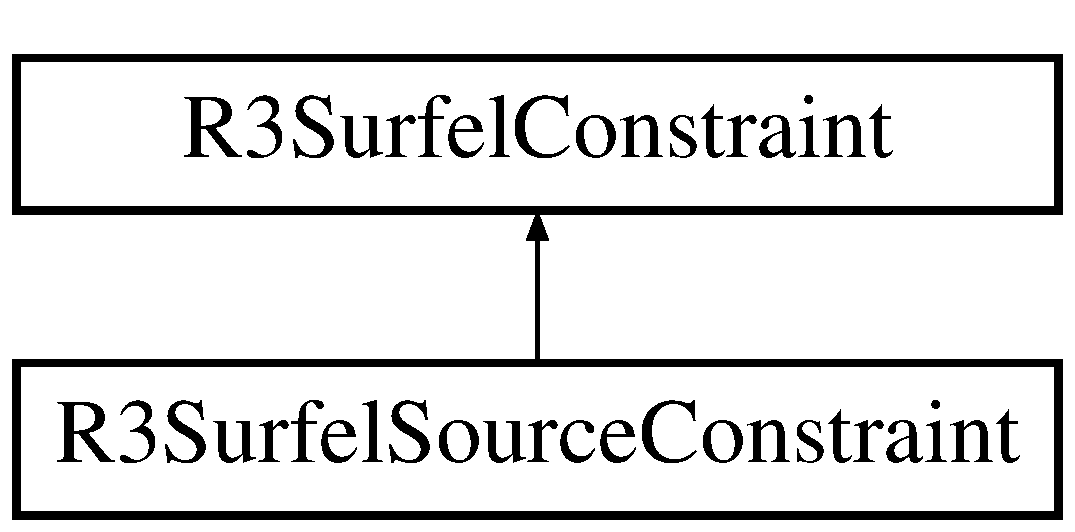
\includegraphics[height=2.000000cm]{class_r3_surfel_source_constraint}
\end{center}
\end{figure}
\subsection*{Public Member Functions}
\begin{DoxyCompactItemize}
\item 
{\bfseries R3\+Surfel\+Source\+Constraint} (R\+N\+Boolean include\+\_\+aerial=T\+R\+UE, R\+N\+Boolean include\+\_\+terrestrial=F\+A\+L\+SE)\hypertarget{class_r3_surfel_source_constraint_a3f631fd9196fbc4a06624c96859029cd}{}\label{class_r3_surfel_source_constraint_a3f631fd9196fbc4a06624c96859029cd}

\item 
virtual int {\bfseries Check} (const \hyperlink{class_r3_surfel_node}{R3\+Surfel\+Node} $\ast$node) const \hypertarget{class_r3_surfel_source_constraint_af137866fa25d71a2ad777c85b348f1cf}{}\label{class_r3_surfel_source_constraint_af137866fa25d71a2ad777c85b348f1cf}

\item 
virtual int {\bfseries Check} (const \hyperlink{class_r3_surfel_block}{R3\+Surfel\+Block} $\ast$block) const \hypertarget{class_r3_surfel_source_constraint_a58a6cae91e174f3eb3be5dae7dbc62ad}{}\label{class_r3_surfel_source_constraint_a58a6cae91e174f3eb3be5dae7dbc62ad}

\item 
virtual int {\bfseries Check} (const \hyperlink{class_r3_surfel_block}{R3\+Surfel\+Block} $\ast$block, const \hyperlink{class_r3_surfel}{R3\+Surfel} $\ast$surfel) const \hypertarget{class_r3_surfel_source_constraint_a681c64091b264120229e174e34c674e1}{}\label{class_r3_surfel_source_constraint_a681c64091b264120229e174e34c674e1}

\end{DoxyCompactItemize}


The documentation for this class was generated from the following files\+:\begin{DoxyCompactItemize}
\item 
R3\+Surfels/R3\+Surfel\+Constraint.\+h\item 
R3\+Surfels/R3\+Surfel\+Constraint.\+cpp\end{DoxyCompactItemize}

\hypertarget{class_r3_surfel_sphere_constraint}{}\section{R3\+Surfel\+Sphere\+Constraint Class Reference}
\label{class_r3_surfel_sphere_constraint}\index{R3\+Surfel\+Sphere\+Constraint@{R3\+Surfel\+Sphere\+Constraint}}
Inheritance diagram for R3\+Surfel\+Sphere\+Constraint\+:\begin{figure}[H]
\begin{center}
\leavevmode
\includegraphics[height=2.000000cm]{class_r3_surfel_sphere_constraint}
\end{center}
\end{figure}
\subsection*{Public Member Functions}
\begin{DoxyCompactItemize}
\item 
{\bfseries R3\+Surfel\+Sphere\+Constraint} (const \hyperlink{class_r3_sphere}{R3\+Sphere} \&sphere)\hypertarget{class_r3_surfel_sphere_constraint_a22c607400417a8c651472e96e6e9091f}{}\label{class_r3_surfel_sphere_constraint_a22c607400417a8c651472e96e6e9091f}

\item 
virtual int {\bfseries Check} (const \hyperlink{class_r3_point}{R3\+Point} \&point) const \hypertarget{class_r3_surfel_sphere_constraint_aef1956edae5f082422a4956b85323c75}{}\label{class_r3_surfel_sphere_constraint_aef1956edae5f082422a4956b85323c75}

\item 
virtual int {\bfseries Check} (const \hyperlink{class_r3_box}{R3\+Box} \&\hyperlink{structbox}{box}) const \hypertarget{class_r3_surfel_sphere_constraint_a5358fbd61492ca2251d3579002a144bf}{}\label{class_r3_surfel_sphere_constraint_a5358fbd61492ca2251d3579002a144bf}

\end{DoxyCompactItemize}


The documentation for this class was generated from the following files\+:\begin{DoxyCompactItemize}
\item 
R3\+Surfels/R3\+Surfel\+Constraint.\+h\item 
R3\+Surfels/R3\+Surfel\+Constraint.\+cpp\end{DoxyCompactItemize}

\hypertarget{class_r3_surfel_tree}{}\section{R3\+Surfel\+Tree Class Reference}
\label{class_r3_surfel_tree}\index{R3\+Surfel\+Tree@{R3\+Surfel\+Tree}}
\subsection*{Public Member Functions}
\begin{DoxyCompactItemize}
\item 
{\bfseries R3\+Surfel\+Tree} (const \hyperlink{class_r3_surfel_tree}{R3\+Surfel\+Tree} \&tree)\hypertarget{class_r3_surfel_tree_a7abf4ad60b589900e60f5f0adc052e30}{}\label{class_r3_surfel_tree_a7abf4ad60b589900e60f5f0adc052e30}

\item 
const \hyperlink{class_r3_box}{R3\+Box} \& {\bfseries B\+Box} (void) const \hypertarget{class_r3_surfel_tree_a08548aa7a55b2dd6cdb2e2c9757c99de}{}\label{class_r3_surfel_tree_a08548aa7a55b2dd6cdb2e2c9757c99de}

\item 
\hyperlink{class_r3_point}{R3\+Point} {\bfseries Centroid} (void) const \hypertarget{class_r3_surfel_tree_abbc3acf02bde5a36a77752f3d87bd815}{}\label{class_r3_surfel_tree_abbc3acf02bde5a36a77752f3d87bd815}

\item 
\hyperlink{class_r3_surfel_scene}{R3\+Surfel\+Scene} $\ast$ {\bfseries Scene} (void) const \hypertarget{class_r3_surfel_tree_a890e7c978b7d0417d6dd16ba6240faba}{}\label{class_r3_surfel_tree_a890e7c978b7d0417d6dd16ba6240faba}

\item 
\hyperlink{class_r3_surfel_database}{R3\+Surfel\+Database} $\ast$ {\bfseries Database} (void) const \hypertarget{class_r3_surfel_tree_a316092d2afa7f30c5cc2abfeee39e297}{}\label{class_r3_surfel_tree_a316092d2afa7f30c5cc2abfeee39e297}

\item 
int {\bfseries N\+Nodes} (void) const \hypertarget{class_r3_surfel_tree_a4940feeccae7de6e760523a4de5c52a3}{}\label{class_r3_surfel_tree_a4940feeccae7de6e760523a4de5c52a3}

\item 
\hyperlink{class_r3_surfel_node}{R3\+Surfel\+Node} $\ast$ {\bfseries Node} (int k) const \hypertarget{class_r3_surfel_tree_ad52c8552b2ec4fc4e58ec59112fef51e}{}\label{class_r3_surfel_tree_ad52c8552b2ec4fc4e58ec59112fef51e}

\item 
\hyperlink{class_r3_surfel_node}{R3\+Surfel\+Node} $\ast$ {\bfseries Find\+Node\+By\+Name} (const char $\ast$node\+\_\+name) const \hypertarget{class_r3_surfel_tree_a4030bcf14d87c959a0b0edffa9a3061b}{}\label{class_r3_surfel_tree_a4030bcf14d87c959a0b0edffa9a3061b}

\item 
\hyperlink{class_r3_surfel_node}{R3\+Surfel\+Node} $\ast$ {\bfseries Root\+Node} (void) const \hypertarget{class_r3_surfel_tree_a282fdf7fed3b62812c157bb9c7fcf381}{}\label{class_r3_surfel_tree_a282fdf7fed3b62812c157bb9c7fcf381}

\item 
void {\bfseries Insert\+Node} (\hyperlink{class_r3_surfel_node}{R3\+Surfel\+Node} $\ast$node, \hyperlink{class_r3_surfel_node}{R3\+Surfel\+Node} $\ast$parent)\hypertarget{class_r3_surfel_tree_a113928fb8f7eafaa88c29275c05c5a1b}{}\label{class_r3_surfel_tree_a113928fb8f7eafaa88c29275c05c5a1b}

\item 
void {\bfseries Remove\+Node} (\hyperlink{class_r3_surfel_node}{R3\+Surfel\+Node} $\ast$node)\hypertarget{class_r3_surfel_tree_aa83d466eaf1ed6e340665acd50d3f097}{}\label{class_r3_surfel_tree_aa83d466eaf1ed6e340665acd50d3f097}

\item 
virtual int {\bfseries Split\+Node} (\hyperlink{class_r3_surfel_node}{R3\+Surfel\+Node} $\ast$node, int max\+\_\+parts\+\_\+per\+\_\+node=64, int max\+\_\+blocks\+\_\+per\+\_\+node=64, R\+N\+Scalar max\+\_\+leaf\+\_\+complexity=1024 $\ast$1024, R\+N\+Scalar max\+\_\+block\+\_\+complexity=1024 $\ast$1024, R\+N\+Length max\+\_\+leaf\+\_\+extent=0, R\+N\+Length max\+\_\+block\+\_\+extent=0, int max\+\_\+levels=64)\hypertarget{class_r3_surfel_tree_a2bc5a8ce8c56a0a2e802e9d51b54b0ba}{}\label{class_r3_surfel_tree_a2bc5a8ce8c56a0a2e802e9d51b54b0ba}

\item 
virtual int {\bfseries Split\+Nodes} (\hyperlink{class_r3_surfel_node}{R3\+Surfel\+Node} $\ast$node, int max\+\_\+parts\+\_\+per\+\_\+node=64, int max\+\_\+blocks\+\_\+per\+\_\+node=64, R\+N\+Scalar max\+\_\+leaf\+\_\+complexity=1024 $\ast$1024, R\+N\+Scalar max\+\_\+block\+\_\+complexity=1024 $\ast$1024, R\+N\+Length max\+\_\+leaf\+\_\+extent=0, R\+N\+Length max\+\_\+block\+\_\+extent=0, int max\+\_\+levels=64)\hypertarget{class_r3_surfel_tree_a42f8c29fb52d5bbfeea2a729d03f9341}{}\label{class_r3_surfel_tree_a42f8c29fb52d5bbfeea2a729d03f9341}

\item 
virtual int {\bfseries Split\+Nodes} (int max\+\_\+parts\+\_\+per\+\_\+node=64, int max\+\_\+blocks\+\_\+per\+\_\+node=64, R\+N\+Scalar max\+\_\+leaf\+\_\+complexity=1024 $\ast$1024, R\+N\+Scalar max\+\_\+block\+\_\+complexity=1024 $\ast$1024, R\+N\+Length max\+\_\+leaf\+\_\+extent=0, R\+N\+Length max\+\_\+block\+\_\+extent=0, int max\+\_\+levels=64)\hypertarget{class_r3_surfel_tree_a66ab3a40ccbbaa0651cdb1e062ed160a}{}\label{class_r3_surfel_tree_a66ab3a40ccbbaa0651cdb1e062ed160a}

\item 
virtual int {\bfseries Split\+Nodes} (\hyperlink{class_r3_surfel_point_set}{R3\+Surfel\+Point\+Set} \&pointset, \hyperlink{class_r_n_array}{R\+N\+Array}$<$ \hyperlink{class_r3_surfel_node}{R3\+Surfel\+Node} $\ast$ $>$ $\ast$nodesA=N\+U\+LL, \hyperlink{class_r_n_array}{R\+N\+Array}$<$ \hyperlink{class_r3_surfel_node}{R3\+Surfel\+Node} $\ast$ $>$ $\ast$nodesB=N\+U\+LL)\hypertarget{class_r3_surfel_tree_abaff7ce6d22daba6872acde1d7ba8629}{}\label{class_r3_surfel_tree_abaff7ce6d22daba6872acde1d7ba8629}

\item 
virtual int {\bfseries Split\+Leaf\+Nodes} (\hyperlink{class_r3_surfel_node}{R3\+Surfel\+Node} $\ast$node, const \hyperlink{class_r3_surfel_constraint}{R3\+Surfel\+Constraint} \&constraint, \hyperlink{class_r_n_array}{R\+N\+Array}$<$ \hyperlink{class_r3_surfel_node}{R3\+Surfel\+Node} $\ast$ $>$ $\ast$nodesA=N\+U\+LL, \hyperlink{class_r_n_array}{R\+N\+Array}$<$ \hyperlink{class_r3_surfel_node}{R3\+Surfel\+Node} $\ast$ $>$ $\ast$nodesB=N\+U\+LL)\hypertarget{class_r3_surfel_tree_a2c9ddd55c0493d96c1cfad1edfd37cb3}{}\label{class_r3_surfel_tree_a2c9ddd55c0493d96c1cfad1edfd37cb3}

\item 
virtual int {\bfseries Split\+Leaf\+Nodes} (const \hyperlink{class_r3_surfel_constraint}{R3\+Surfel\+Constraint} \&constraint, \hyperlink{class_r_n_array}{R\+N\+Array}$<$ \hyperlink{class_r3_surfel_node}{R3\+Surfel\+Node} $\ast$ $>$ $\ast$nodesA=N\+U\+LL, \hyperlink{class_r_n_array}{R\+N\+Array}$<$ \hyperlink{class_r3_surfel_node}{R3\+Surfel\+Node} $\ast$ $>$ $\ast$nodesB=N\+U\+LL)\hypertarget{class_r3_surfel_tree_a1935349f9ae274fc8654b292323e3a74}{}\label{class_r3_surfel_tree_a1935349f9ae274fc8654b292323e3a74}

\item 
int {\bfseries Create\+Multiresolution\+Nodes} (R\+N\+Scalar min\+\_\+complexity=8, R\+N\+Scalar min\+\_\+resolution=1.\+0, R\+N\+Scalar min\+\_\+multiresolution\+\_\+factor=0.\+25)\hypertarget{class_r3_surfel_tree_a21f1a3d9145c737ee134c90a95e51a3b}{}\label{class_r3_surfel_tree_a21f1a3d9145c737ee134c90a95e51a3b}

\item 
virtual int {\bfseries Split\+Blocks} (\hyperlink{class_r3_surfel_node}{R3\+Surfel\+Node} $\ast$node, R\+N\+Scalar max\+\_\+complexity, R\+N\+Scalar max\+\_\+extent)\hypertarget{class_r3_surfel_tree_a8d10bbefe220c1706f38f12ee126a2b1}{}\label{class_r3_surfel_tree_a8d10bbefe220c1706f38f12ee126a2b1}

\item 
virtual int {\bfseries Split\+Blocks} (\hyperlink{class_r3_surfel_node}{R3\+Surfel\+Node} $\ast$node, \hyperlink{class_r3_surfel_point_set}{R3\+Surfel\+Point\+Set} \&pointset, \hyperlink{class_r_n_array}{R\+N\+Array}$<$ \hyperlink{class_r3_surfel_block}{R3\+Surfel\+Block} $\ast$ $>$ $\ast$blocksA=N\+U\+LL, \hyperlink{class_r_n_array}{R\+N\+Array}$<$ \hyperlink{class_r3_surfel_block}{R3\+Surfel\+Block} $\ast$ $>$ $\ast$blocksB=N\+U\+LL)\hypertarget{class_r3_surfel_tree_a23e873aac8d09da7708b1d2c22edc2cf}{}\label{class_r3_surfel_tree_a23e873aac8d09da7708b1d2c22edc2cf}

\item 
virtual int {\bfseries Split\+Block} (\hyperlink{class_r3_surfel_node}{R3\+Surfel\+Node} $\ast$node, \hyperlink{class_r3_surfel_block}{R3\+Surfel\+Block} $\ast$block, const \hyperlink{class_r3_surfel_constraint}{R3\+Surfel\+Constraint} \&constraint, \hyperlink{class_r3_surfel_block}{R3\+Surfel\+Block} $\ast$$\ast$blockA=N\+U\+LL, \hyperlink{class_r3_surfel_block}{R3\+Surfel\+Block} $\ast$$\ast$blockB=N\+U\+LL)\hypertarget{class_r3_surfel_tree_a467595048f9a7a738ceddbde9a00ff1a}{}\label{class_r3_surfel_tree_a467595048f9a7a738ceddbde9a00ff1a}

\item 
virtual int {\bfseries Split\+Blocks} (\hyperlink{class_r3_surfel_node}{R3\+Surfel\+Node} $\ast$node, const \hyperlink{class_r3_surfel_constraint}{R3\+Surfel\+Constraint} \&constraint, \hyperlink{class_r_n_array}{R\+N\+Array}$<$ \hyperlink{class_r3_surfel_block}{R3\+Surfel\+Block} $\ast$ $>$ $\ast$blocksA=N\+U\+LL, \hyperlink{class_r_n_array}{R\+N\+Array}$<$ \hyperlink{class_r3_surfel_block}{R3\+Surfel\+Block} $\ast$ $>$ $\ast$blocksB=N\+U\+LL)\hypertarget{class_r3_surfel_tree_acdd80a1807e4d535a506cb39328d6440}{}\label{class_r3_surfel_tree_acdd80a1807e4d535a506cb39328d6440}

\item 
virtual int {\bfseries Create\+Multiresolution\+Blocks} (\hyperlink{class_r3_surfel_node}{R3\+Surfel\+Node} $\ast$node, R\+N\+Scalar multiresolution\+\_\+factor=0.\+25, R\+N\+Scalar max\+\_\+complexity=0, R\+N\+Scalar max\+\_\+resolution=0)\hypertarget{class_r3_surfel_tree_a1be496d5944770dbe284046b85a34fcf}{}\label{class_r3_surfel_tree_a1be496d5944770dbe284046b85a34fcf}

\item 
virtual int {\bfseries Create\+Multiresolution\+Blocks} (R\+N\+Scalar multiresolution\+\_\+factor=0.\+25, R\+N\+Scalar max\+\_\+complexity=0)\hypertarget{class_r3_surfel_tree_a20392a96414cd9f14d7a0f4a10e325b6}{}\label{class_r3_surfel_tree_a20392a96414cd9f14d7a0f4a10e325b6}

\item 
virtual void {\bfseries Draw} (\hyperlink{class_r_n_flags}{R\+N\+Flags} flags=R3\+\_\+\+S\+U\+R\+F\+E\+L\+\_\+\+D\+E\+F\+A\+U\+L\+T\+\_\+\+D\+R\+A\+W\+\_\+\+F\+L\+A\+GS) const \hypertarget{class_r3_surfel_tree_a8f51db85191ff2292d5aaf42428029fb}{}\label{class_r3_surfel_tree_a8f51db85191ff2292d5aaf42428029fb}

\item 
virtual void {\bfseries Print} (F\+I\+LE $\ast$fp=N\+U\+LL, const char $\ast$prefix=N\+U\+LL, const char $\ast$suffix=N\+U\+LL) const \hypertarget{class_r3_surfel_tree_af72214b2fc4824eb9def832d88075ead}{}\label{class_r3_surfel_tree_af72214b2fc4824eb9def832d88075ead}

\end{DoxyCompactItemize}
\subsection*{Protected Member Functions}
\begin{DoxyCompactItemize}
\item 
void {\bfseries Update\+After\+Insert} (\hyperlink{class_r3_surfel_scene}{R3\+Surfel\+Scene} $\ast$scene)\hypertarget{class_r3_surfel_tree_af7fedd8d434370aa170fcd761e8bde7b}{}\label{class_r3_surfel_tree_af7fedd8d434370aa170fcd761e8bde7b}

\item 
void {\bfseries Update\+Before\+Remove} (\hyperlink{class_r3_surfel_scene}{R3\+Surfel\+Scene} $\ast$scene)\hypertarget{class_r3_surfel_tree_a7aba29374236a3268b170b067a719d6a}{}\label{class_r3_surfel_tree_a7aba29374236a3268b170b067a719d6a}

\end{DoxyCompactItemize}
\subsection*{Protected Attributes}
\begin{DoxyCompactItemize}
\item 
\hyperlink{class_r3_surfel_scene}{R3\+Surfel\+Scene} $\ast$ {\bfseries scene}\hypertarget{class_r3_surfel_tree_a539c3395878b18d64161abc9a031945d}{}\label{class_r3_surfel_tree_a539c3395878b18d64161abc9a031945d}

\item 
\hyperlink{class_r3_surfel_database}{R3\+Surfel\+Database} $\ast$ {\bfseries database}\hypertarget{class_r3_surfel_tree_ac7ffc4e198f2d4849009b91cde00cfa9}{}\label{class_r3_surfel_tree_ac7ffc4e198f2d4849009b91cde00cfa9}

\item 
\hyperlink{class_r_n_array}{R\+N\+Array}$<$ \hyperlink{class_r3_surfel_node}{R3\+Surfel\+Node} $\ast$ $>$ {\bfseries nodes}\hypertarget{class_r3_surfel_tree_ae5067b7c9cba8c66d3fd79c6b23c3d11}{}\label{class_r3_surfel_tree_ae5067b7c9cba8c66d3fd79c6b23c3d11}

\end{DoxyCompactItemize}
\subsection*{Friends}
\begin{DoxyCompactItemize}
\item 
class {\bfseries R3\+Surfel\+Scene}\hypertarget{class_r3_surfel_tree_af9bb32c0eac7d1d54787bbc6b44586b6}{}\label{class_r3_surfel_tree_af9bb32c0eac7d1d54787bbc6b44586b6}

\end{DoxyCompactItemize}


The documentation for this class was generated from the following files\+:\begin{DoxyCompactItemize}
\item 
R3\+Surfels/R3\+Surfel\+Tree.\+h\item 
R3\+Surfels/R3\+Surfel\+Tree.\+cpp\end{DoxyCompactItemize}

\hypertarget{class_r3_transformation}{}\section{R3\+Transformation Class Reference}
\label{class_r3_transformation}\index{R3\+Transformation@{R3\+Transformation}}
Inheritance diagram for R3\+Transformation\+:\begin{figure}[H]
\begin{center}
\leavevmode
\includegraphics[height=2.000000cm]{class_r3_transformation}
\end{center}
\end{figure}
\subsection*{Public Member Functions}
\begin{DoxyCompactItemize}
\item 
virtual const R\+N\+Boolean {\bfseries Is\+Mirrored} (void) const \hypertarget{class_r3_transformation_a02567b2778174d98cd617abb6ed7d9b4}{}\label{class_r3_transformation_a02567b2778174d98cd617abb6ed7d9b4}

\item 
virtual const R\+N\+Boolean {\bfseries Is\+Linear} (void) const \hypertarget{class_r3_transformation_a1e89e187e8b63f05a0ee6dfc835aa8ab}{}\label{class_r3_transformation_a1e89e187e8b63f05a0ee6dfc835aa8ab}

\item 
virtual const R\+N\+Boolean {\bfseries Is\+Affine} (void) const \hypertarget{class_r3_transformation_a85059c0b5b40a62ce97c92a957ffc844}{}\label{class_r3_transformation_a85059c0b5b40a62ce97c92a957ffc844}

\item 
virtual const R\+N\+Boolean {\bfseries Is\+Isotropic} (void) const \hypertarget{class_r3_transformation_af0690239eae5c267eff275d35acd4e44}{}\label{class_r3_transformation_af0690239eae5c267eff275d35acd4e44}

\item 
virtual void {\bfseries Apply} (\hyperlink{class_r3_vector}{R3\+Vector} \&vector) const  =0\hypertarget{class_r3_transformation_aca1a29ad882a1eebcd779df887a65eaa}{}\label{class_r3_transformation_aca1a29ad882a1eebcd779df887a65eaa}

\item 
virtual void {\bfseries Apply} (\hyperlink{class_r3_point}{R3\+Point} \&point) const  =0\hypertarget{class_r3_transformation_a53942ad60b39d77749be3c966db67a77}{}\label{class_r3_transformation_a53942ad60b39d77749be3c966db67a77}

\item 
virtual void {\bfseries Apply} (\hyperlink{class_r3_transformation}{R3\+Transformation} \&transformation) const  =0\hypertarget{class_r3_transformation_a47f7e751acd461363a7b31bfe6062199}{}\label{class_r3_transformation_a47f7e751acd461363a7b31bfe6062199}

\item 
virtual void {\bfseries Apply} (\hyperlink{class_r3_affine}{R3\+Affine} \&affine) const  =0\hypertarget{class_r3_transformation_a56e01a4f3d12f254192dacf340ced6cd}{}\label{class_r3_transformation_a56e01a4f3d12f254192dacf340ced6cd}

\item 
virtual void {\bfseries Apply\+Inverse} (\hyperlink{class_r3_vector}{R3\+Vector} \&vector) const  =0\hypertarget{class_r3_transformation_a0cc945f3871e62539e463ef01e62b2b3}{}\label{class_r3_transformation_a0cc945f3871e62539e463ef01e62b2b3}

\item 
virtual void {\bfseries Apply\+Inverse} (\hyperlink{class_r3_point}{R3\+Point} \&point) const  =0\hypertarget{class_r3_transformation_ae26c82f934acdee40328516e0cb16c93}{}\label{class_r3_transformation_ae26c82f934acdee40328516e0cb16c93}

\item 
virtual void {\bfseries Apply\+Inverse} (\hyperlink{class_r3_transformation}{R3\+Transformation} \&transformation) const  =0\hypertarget{class_r3_transformation_abaa5d37d45834188dd9d0de204db02f3}{}\label{class_r3_transformation_abaa5d37d45834188dd9d0de204db02f3}

\item 
virtual void {\bfseries Apply\+Inverse} (\hyperlink{class_r3_affine}{R3\+Affine} \&affine) const  =0\hypertarget{class_r3_transformation_a80f3a0b0766f00a2b1988338a2757437}{}\label{class_r3_transformation_a80f3a0b0766f00a2b1988338a2757437}

\item 
virtual void {\bfseries Apply\+Inverse\+Transpose} (\hyperlink{class_r3_vector}{R3\+Vector} \&vector) const  =0\hypertarget{class_r3_transformation_a3ba6f0db517b367f932e256695faf019}{}\label{class_r3_transformation_a3ba6f0db517b367f932e256695faf019}

\item 
virtual void {\bfseries Apply\+Transpose} (\hyperlink{class_r3_vector}{R3\+Vector} \&vector) const  =0\hypertarget{class_r3_transformation_aefbcc2e7065cb996096a0a530159124f}{}\label{class_r3_transformation_aefbcc2e7065cb996096a0a530159124f}

\item 
virtual void {\bfseries Reset} (const \hyperlink{class_r3_transformation}{R3\+Transformation} \&transformation)=0\hypertarget{class_r3_transformation_a0fbb6253fad9ebef1a2a2a8665c6aea1}{}\label{class_r3_transformation_a0fbb6253fad9ebef1a2a2a8665c6aea1}

\item 
virtual void {\bfseries Transform} (const \hyperlink{class_r3_transformation}{R3\+Transformation} \&transformation)=0\hypertarget{class_r3_transformation_a1da4e6e350f20020e84f326097823b85}{}\label{class_r3_transformation_a1da4e6e350f20020e84f326097823b85}

\item 
virtual void {\bfseries Inverse\+Transform} (const \hyperlink{class_r3_transformation}{R3\+Transformation} \&transformation)=0\hypertarget{class_r3_transformation_aaf8083034538d0c617b0f2f4a47cffd3}{}\label{class_r3_transformation_aaf8083034538d0c617b0f2f4a47cffd3}

\item 
virtual void {\bfseries Load} (void) const  =0\hypertarget{class_r3_transformation_a3d8367c81ba92b5a03c5e76323394790}{}\label{class_r3_transformation_a3d8367c81ba92b5a03c5e76323394790}

\item 
virtual void {\bfseries Draw} (void) const  =0\hypertarget{class_r3_transformation_a87bc7bb94a7b45041afbb3c245db3ed6}{}\label{class_r3_transformation_a87bc7bb94a7b45041afbb3c245db3ed6}

\item 
virtual void {\bfseries Push} (void) const  =0\hypertarget{class_r3_transformation_a12ebcb9129ffa19656406e5f21fcc2d7}{}\label{class_r3_transformation_a12ebcb9129ffa19656406e5f21fcc2d7}

\item 
virtual void {\bfseries Pop} (void) const  =0\hypertarget{class_r3_transformation_a65b18be6557b417d31c7e859499c82f0}{}\label{class_r3_transformation_a65b18be6557b417d31c7e859499c82f0}

\item 
virtual const R\+N\+Scalar {\bfseries Scale\+Factor} (void) const \hypertarget{class_r3_transformation_adb79cd60f0e893cde9f09a3e31c816cd}{}\label{class_r3_transformation_adb79cd60f0e893cde9f09a3e31c816cd}

\end{DoxyCompactItemize}


The documentation for this class was generated from the following files\+:\begin{DoxyCompactItemize}
\item 
R3\+Shapes/R3\+Xform.\+h\item 
R3\+Shapes/R3\+Xform.\+cpp\end{DoxyCompactItemize}

\hypertarget{class_r3_triad}{}\section{R3\+Triad Class Reference}
\label{class_r3_triad}\index{R3\+Triad@{R3\+Triad}}
\subsection*{Public Member Functions}
\begin{DoxyCompactItemize}
\item 
{\bfseries R3\+Triad} (const \hyperlink{class_r3_triad}{R3\+Triad} \&triad)\hypertarget{class_r3_triad_a4e5e69f9b5ea9a2ea67269be589fda2d}{}\label{class_r3_triad_a4e5e69f9b5ea9a2ea67269be589fda2d}

\item 
{\bfseries R3\+Triad} (const \hyperlink{class_r3_vector}{R3\+Vector} \&xaxis, const \hyperlink{class_r3_vector}{R3\+Vector} \&yaxis, const \hyperlink{class_r3_vector}{R3\+Vector} \&zaxis)\hypertarget{class_r3_triad_a80b6557359ea92feb027538c8ad54256}{}\label{class_r3_triad_a80b6557359ea92feb027538c8ad54256}

\item 
{\bfseries R3\+Triad} (const \hyperlink{class_r3_vector}{R3\+Vector} \&towards, const \hyperlink{class_r3_vector}{R3\+Vector} \&up)\hypertarget{class_r3_triad_aeb0e5a556e39e0e5ac5e6e767571a1cb}{}\label{class_r3_triad_aeb0e5a556e39e0e5ac5e6e767571a1cb}

\item 
const \hyperlink{class_r4_matrix}{R4\+Matrix} {\bfseries Matrix} (void) const \hypertarget{class_r3_triad_a38d0d3c029e713d28e0756dae94c2c59}{}\label{class_r3_triad_a38d0d3c029e713d28e0756dae94c2c59}

\item 
const \hyperlink{class_r4_matrix}{R4\+Matrix} {\bfseries Inverse\+Matrix} (void) const \hypertarget{class_r3_triad_a67a6399fa41010532ddb299c32589def}{}\label{class_r3_triad_a67a6399fa41010532ddb299c32589def}

\item 
const \hyperlink{class_r3_vector}{R3\+Vector} \& {\bfseries Axis} (R\+N\+Dimension dim) const \hypertarget{class_r3_triad_a48f45e93ca512140f4574d1d9b66ed7e}{}\label{class_r3_triad_a48f45e93ca512140f4574d1d9b66ed7e}

\item 
const \hyperlink{class_r3_vector}{R3\+Vector} \& {\bfseries operator\mbox{[}$\,$\mbox{]}} (R\+N\+Dimension dim) const \hypertarget{class_r3_triad_a8a30cc925b606806691d218715a55136}{}\label{class_r3_triad_a8a30cc925b606806691d218715a55136}

\item 
const R\+N\+Boolean {\bfseries operator==} (const \hyperlink{class_r3_triad}{R3\+Triad} \&triad) const \hypertarget{class_r3_triad_a00bccce11a563cee49da9c707b6bad67}{}\label{class_r3_triad_a00bccce11a563cee49da9c707b6bad67}

\item 
const R\+N\+Boolean {\bfseries operator!=} (const \hyperlink{class_r3_triad}{R3\+Triad} \&triad) const \hypertarget{class_r3_triad_a86593eb8e77ef8bff13643d242e7475e}{}\label{class_r3_triad_a86593eb8e77ef8bff13643d242e7475e}

\item 
void {\bfseries Normalize} (void)\hypertarget{class_r3_triad_ab813ec5d5da8d37c711b77dce31c604b}{}\label{class_r3_triad_ab813ec5d5da8d37c711b77dce31c604b}

\item 
void {\bfseries Rotate} (R\+N\+Axis axis, R\+N\+Angle radians)\hypertarget{class_r3_triad_a68c5d2d872da08450d28930c0e44aba7}{}\label{class_r3_triad_a68c5d2d872da08450d28930c0e44aba7}

\item 
void {\bfseries Rotate} (const \hyperlink{class_r3_vector}{R3\+Vector} \&vector, R\+N\+Angle radians)\hypertarget{class_r3_triad_aacafe46c8edcd3f62fd52ea84f3874c4}{}\label{class_r3_triad_aacafe46c8edcd3f62fd52ea84f3874c4}

\item 
void {\bfseries Rotate} (const \hyperlink{class_r3_vector}{R3\+Vector} \&from, const \hyperlink{class_r3_vector}{R3\+Vector} \&to)\hypertarget{class_r3_triad_a0d948df1ca034335c0345087adc7e000}{}\label{class_r3_triad_a0d948df1ca034335c0345087adc7e000}

\item 
void {\bfseries Mirror} (const \hyperlink{class_r3_plane}{R3\+Plane} \&plane)\hypertarget{class_r3_triad_a3b7c1d8c7684e43bebe062d8f3c3c6fa}{}\label{class_r3_triad_a3b7c1d8c7684e43bebe062d8f3c3c6fa}

\item 
void {\bfseries Transform} (const \hyperlink{class_r3_transformation}{R3\+Transformation} \&transformation)\hypertarget{class_r3_triad_ab8eab99179c15978f1198871194abed2}{}\label{class_r3_triad_ab8eab99179c15978f1198871194abed2}

\item 
void {\bfseries Inverse\+Transform} (const \hyperlink{class_r3_transformation}{R3\+Transformation} \&transformation)\hypertarget{class_r3_triad_a6049666f25055f918ceda966296d1b71}{}\label{class_r3_triad_a6049666f25055f918ceda966296d1b71}

\item 
\hyperlink{class_r3_triad}{R3\+Triad} \& {\bfseries operator=} (const \hyperlink{class_r3_triad}{R3\+Triad} \&triad)\hypertarget{class_r3_triad_a04ea745b56fab200405d2245e361de08}{}\label{class_r3_triad_a04ea745b56fab200405d2245e361de08}

\item 
void {\bfseries Draw} (void) const \hypertarget{class_r3_triad_a97b3418977e6ecb792083cc5f8800f08}{}\label{class_r3_triad_a97b3418977e6ecb792083cc5f8800f08}

\item 
void {\bfseries Outline} (void) const \hypertarget{class_r3_triad_ab9c3fd6aac77df8af82d85934f423a08}{}\label{class_r3_triad_ab9c3fd6aac77df8af82d85934f423a08}

\end{DoxyCompactItemize}


The documentation for this class was generated from the following files\+:\begin{DoxyCompactItemize}
\item 
R3\+Shapes/R3\+Triad.\+h\item 
R3\+Shapes/R3\+Draw.\+cpp\item 
R3\+Shapes/R3\+Triad.\+cpp\end{DoxyCompactItemize}

\hypertarget{class_r3_triangle}{}\section{R3\+Triangle Class Reference}
\label{class_r3_triangle}\index{R3\+Triangle@{R3\+Triangle}}
Inheritance diagram for R3\+Triangle\+:\begin{figure}[H]
\begin{center}
\leavevmode
\includegraphics[height=3.000000cm]{class_r3_triangle}
\end{center}
\end{figure}
\subsection*{Public Member Functions}
\begin{DoxyCompactItemize}
\item 
{\bfseries R3\+Triangle} (const \hyperlink{class_r3_triangle}{R3\+Triangle} \&triangle)\hypertarget{class_r3_triangle_aede76a868d13ee80e427900b31d3c283}{}\label{class_r3_triangle_aede76a868d13ee80e427900b31d3c283}

\item 
{\bfseries R3\+Triangle} (\hyperlink{class_r3_triangle_vertex}{R3\+Triangle\+Vertex} $\ast$v0, \hyperlink{class_r3_triangle_vertex}{R3\+Triangle\+Vertex} $\ast$v1, \hyperlink{class_r3_triangle_vertex}{R3\+Triangle\+Vertex} $\ast$v2)\hypertarget{class_r3_triangle_a5d8545a2e469ef81802ba91d98aec619}{}\label{class_r3_triangle_a5d8545a2e469ef81802ba91d98aec619}

\item 
{\bfseries R3\+Triangle} (\hyperlink{class_r3_triangle_vertex}{R3\+Triangle\+Vertex} $\ast$vertices\mbox{[}3\mbox{]})\hypertarget{class_r3_triangle_aa1658f56ed03b658990986bb3664a792}{}\label{class_r3_triangle_aa1658f56ed03b658990986bb3664a792}

\item 
\hyperlink{class_r3_triangle_vertex}{R3\+Triangle\+Vertex} $\ast$ {\bfseries Vertex} (int index) const \hypertarget{class_r3_triangle_af270909154d10a603b650fafbd806fc5}{}\label{class_r3_triangle_af270909154d10a603b650fafbd806fc5}

\item 
\hyperlink{class_r3_triangle_vertex}{R3\+Triangle\+Vertex} $\ast$ {\bfseries V0} (void) const \hypertarget{class_r3_triangle_ad3c47eeb4f1b893684da3484d3145027}{}\label{class_r3_triangle_ad3c47eeb4f1b893684da3484d3145027}

\item 
\hyperlink{class_r3_triangle_vertex}{R3\+Triangle\+Vertex} $\ast$ {\bfseries V1} (void) const \hypertarget{class_r3_triangle_ab4dba1ad4c077d08bed8d3f5e222db08}{}\label{class_r3_triangle_ab4dba1ad4c077d08bed8d3f5e222db08}

\item 
\hyperlink{class_r3_triangle_vertex}{R3\+Triangle\+Vertex} $\ast$ {\bfseries V2} (void) const \hypertarget{class_r3_triangle_aac0b228fc155088e2b48285945a9592d}{}\label{class_r3_triangle_aac0b228fc155088e2b48285945a9592d}

\item 
const \hyperlink{class_r3_plane}{R3\+Plane} \& {\bfseries Plane} (void) const \hypertarget{class_r3_triangle_ac7965ae02971b5378f086b0987ea8d4d}{}\label{class_r3_triangle_ac7965ae02971b5378f086b0987ea8d4d}

\item 
const \hyperlink{class_r3_vector}{R3\+Vector} \& {\bfseries Normal} (void) const \hypertarget{class_r3_triangle_ad44cd8ce46c998a0f75e4349216872c9}{}\label{class_r3_triangle_ad44cd8ce46c998a0f75e4349216872c9}

\item 
const \hyperlink{class_r3_box}{R3\+Box} \& {\bfseries Box} (void) const \hypertarget{class_r3_triangle_add5e129187af577fcd7f42da27965740}{}\label{class_r3_triangle_add5e129187af577fcd7f42da27965740}

\item 
const \hyperlink{class_r_n_flags}{R\+N\+Flags} {\bfseries Flags} (void) const \hypertarget{class_r3_triangle_a1d6a8e72b57bfcb9fa3da6434d107830}{}\label{class_r3_triangle_a1d6a8e72b57bfcb9fa3da6434d107830}

\item 
const R\+N\+Mark {\bfseries Mark} (void) const \hypertarget{class_r3_triangle_aafe16d22d7f111b623ae2e9dad44bbd4}{}\label{class_r3_triangle_aafe16d22d7f111b623ae2e9dad44bbd4}

\item 
const R\+N\+Boolean {\bfseries Is\+Finite} (void) const \hypertarget{class_r3_triangle_a0858d44a26049e898d71bcc046795415}{}\label{class_r3_triangle_a0858d44a26049e898d71bcc046795415}

\item 
const R\+N\+Boolean {\bfseries Is\+Degenerate} (void) const \hypertarget{class_r3_triangle_a4d185bfbdaec8318215fc54e7703a741}{}\label{class_r3_triangle_a4d185bfbdaec8318215fc54e7703a741}

\item 
virtual const R\+N\+Boolean {\bfseries Is\+Point} (void) const \hypertarget{class_r3_triangle_af0769d0efe11a08ff66a69d9fce02f6b}{}\label{class_r3_triangle_af0769d0efe11a08ff66a69d9fce02f6b}

\item 
virtual const R\+N\+Boolean {\bfseries Is\+Linear} (void) const \hypertarget{class_r3_triangle_a4c305ede4425a7005d2b7c08aa2dda79}{}\label{class_r3_triangle_a4c305ede4425a7005d2b7c08aa2dda79}

\item 
virtual const R\+N\+Boolean {\bfseries Is\+Planar} (void) const \hypertarget{class_r3_triangle_a3b163f1d3273a4fbeab7c7d42fb2ad8d}{}\label{class_r3_triangle_a3b163f1d3273a4fbeab7c7d42fb2ad8d}

\item 
virtual const R\+N\+Boolean {\bfseries Is\+Convex} (void) const \hypertarget{class_r3_triangle_ab87ced483dbcd6eccb734e42467c1fc3}{}\label{class_r3_triangle_ab87ced483dbcd6eccb734e42467c1fc3}

\item 
virtual const \hyperlink{class_r_n_interval}{R\+N\+Interval} {\bfseries N\+Facets} (void) const \hypertarget{class_r3_triangle_a13197ef5dd97d23f2a6c14ad9bb571a8}{}\label{class_r3_triangle_a13197ef5dd97d23f2a6c14ad9bb571a8}

\item 
virtual const R\+N\+Length {\bfseries Length} (void) const \hypertarget{class_r3_triangle_a763d740dcab38dfd40ae76ae6c1c678f}{}\label{class_r3_triangle_a763d740dcab38dfd40ae76ae6c1c678f}

\item 
virtual const R\+N\+Area {\bfseries Area} (void) const \hypertarget{class_r3_triangle_ac7664ca6459ddecd58a5127939798993}{}\label{class_r3_triangle_ac7664ca6459ddecd58a5127939798993}

\item 
virtual const \hyperlink{class_r3_point}{R3\+Point} {\bfseries Centroid} (void) const \hypertarget{class_r3_triangle_a91c652c6c2446bfe8350d06f8199d355}{}\label{class_r3_triangle_a91c652c6c2446bfe8350d06f8199d355}

\item 
virtual const \hyperlink{class_r3_point}{R3\+Point} {\bfseries Closest\+Point} (const \hyperlink{class_r3_point}{R3\+Point} \&point) const \hypertarget{class_r3_triangle_a671124bdb54f9075ec6c4f932898a048}{}\label{class_r3_triangle_a671124bdb54f9075ec6c4f932898a048}

\item 
virtual const \hyperlink{class_r3_point}{R3\+Point} {\bfseries Furthest\+Point} (const \hyperlink{class_r3_point}{R3\+Point} \&point) const \hypertarget{class_r3_triangle_a364ded2e250548137a968d733df55641}{}\label{class_r3_triangle_a364ded2e250548137a968d733df55641}

\item 
virtual const \hyperlink{class_r3_shape}{R3\+Shape} \& {\bfseries B\+Shape} (void) const \hypertarget{class_r3_triangle_a3c0a4431ba6aae2d8af376f42379d889}{}\label{class_r3_triangle_a3c0a4431ba6aae2d8af376f42379d889}

\item 
virtual const \hyperlink{class_r3_box}{R3\+Box} {\bfseries B\+Box} (void) const \hypertarget{class_r3_triangle_a8c91bbfd58fb27f049e7476332ff3431}{}\label{class_r3_triangle_a8c91bbfd58fb27f049e7476332ff3431}

\item 
virtual const \hyperlink{class_r3_sphere}{R3\+Sphere} {\bfseries B\+Sphere} (void) const \hypertarget{class_r3_triangle_a0f82b8786cb875fc2d428a849ed18a23}{}\label{class_r3_triangle_a0f82b8786cb875fc2d428a849ed18a23}

\item 
virtual void {\bfseries Flip} (void)\hypertarget{class_r3_triangle_a573a5268c792b47a35e5f6437b665f17}{}\label{class_r3_triangle_a573a5268c792b47a35e5f6437b665f17}

\item 
virtual void {\bfseries Transform} (const \hyperlink{class_r3_transformation}{R3\+Transformation} \&transformation)\hypertarget{class_r3_triangle_a730bccc677aaa67e2f177c48cf2d7216}{}\label{class_r3_triangle_a730bccc677aaa67e2f177c48cf2d7216}

\item 
virtual void {\bfseries Mirror} (const \hyperlink{class_r3_plane}{R3\+Plane} \&plane)\hypertarget{class_r3_triangle_aa250f51abf0ccfcd8d7082459a1c5d3b}{}\label{class_r3_triangle_aa250f51abf0ccfcd8d7082459a1c5d3b}

\item 
virtual void {\bfseries Reset} (\hyperlink{class_r3_triangle_vertex}{R3\+Triangle\+Vertex} $\ast$v1, \hyperlink{class_r3_triangle_vertex}{R3\+Triangle\+Vertex} $\ast$v2, \hyperlink{class_r3_triangle_vertex}{R3\+Triangle\+Vertex} $\ast$v3)\hypertarget{class_r3_triangle_aaf67e47d486d2ebe54471cee222a683a}{}\label{class_r3_triangle_aaf67e47d486d2ebe54471cee222a683a}

\item 
virtual void {\bfseries Reset} (\hyperlink{class_r3_triangle_vertex}{R3\+Triangle\+Vertex} $\ast$vertices\mbox{[}3\mbox{]})\hypertarget{class_r3_triangle_ad36d2c040d44a7f94cc31ac64da02719}{}\label{class_r3_triangle_ad36d2c040d44a7f94cc31ac64da02719}

\item 
virtual void {\bfseries Set\+Mark} (R\+N\+Mark mark)\hypertarget{class_r3_triangle_aa529e1bc6f7797b3b53679f8d4d4f640}{}\label{class_r3_triangle_aa529e1bc6f7797b3b53679f8d4d4f640}

\item 
virtual void {\bfseries Update} (void)\hypertarget{class_r3_triangle_a09e3ad912f617a32e599a729043a2d0c}{}\label{class_r3_triangle_a09e3ad912f617a32e599a729043a2d0c}

\item 
virtual void {\bfseries Draw} (const \hyperlink{class_r_n_flags}{R3\+Draw\+Flags} draw\+\_\+flags=R3\+\_\+\+D\+E\+F\+A\+U\+L\+T\+\_\+\+D\+R\+A\+W\+\_\+\+F\+L\+A\+GS) const \hypertarget{class_r3_triangle_a0415686c5cba40a6e39217beab808d10}{}\label{class_r3_triangle_a0415686c5cba40a6e39217beab808d10}

\item 
\hyperlink{class_r3_triangle}{R3\+Triangle} {\bfseries operator-\/} (void) const \hypertarget{class_r3_triangle_abe0aea5253de3754712fa7d30bdbc4ab}{}\label{class_r3_triangle_abe0aea5253de3754712fa7d30bdbc4ab}

\item 
{\bfseries R\+N\+\_\+\+C\+L\+A\+S\+S\+\_\+\+T\+Y\+P\+E\+\_\+\+D\+E\+C\+L\+A\+R\+A\+T\+I\+O\+NS} (\hyperlink{class_r3_triangle}{R3\+Triangle})\hypertarget{class_r3_triangle_a6ab4e614ff35a2ec6c3900d3f36eaa15}{}\label{class_r3_triangle_a6ab4e614ff35a2ec6c3900d3f36eaa15}

\item 
{\bfseries R3\+\_\+\+S\+H\+A\+P\+E\+\_\+\+R\+E\+L\+A\+T\+I\+O\+N\+S\+H\+I\+P\+\_\+\+D\+E\+C\+L\+A\+R\+A\+T\+I\+O\+NS} (\hyperlink{class_r3_triangle}{R3\+Triangle})\hypertarget{class_r3_triangle_a144aab96542103c61ff053832ae4cbaa}{}\label{class_r3_triangle_a144aab96542103c61ff053832ae4cbaa}

\end{DoxyCompactItemize}


The documentation for this class was generated from the following files\+:\begin{DoxyCompactItemize}
\item 
R3\+Shapes/R3\+Triangle.\+h\item 
R3\+Shapes/R3\+Draw.\+cpp\item 
R3\+Shapes/R3\+Triangle.\+cpp\end{DoxyCompactItemize}

\hypertarget{class_r3_triangle_array}{}\section{R3\+Triangle\+Array Class Reference}
\label{class_r3_triangle_array}\index{R3\+Triangle\+Array@{R3\+Triangle\+Array}}
Inheritance diagram for R3\+Triangle\+Array\+:\begin{figure}[H]
\begin{center}
\leavevmode
\includegraphics[height=3.000000cm]{class_r3_triangle_array}
\end{center}
\end{figure}
\subsection*{Public Member Functions}
\begin{DoxyCompactItemize}
\item 
{\bfseries R3\+Triangle\+Array} (const \hyperlink{class_r3_triangle_array}{R3\+Triangle\+Array} \&array)\hypertarget{class_r3_triangle_array_ac582af694dddaa082bcb51eb6d3354ed}{}\label{class_r3_triangle_array_ac582af694dddaa082bcb51eb6d3354ed}

\item 
{\bfseries R3\+Triangle\+Array} (const \hyperlink{class_r_n_array}{R\+N\+Array}$<$ \hyperlink{class_r3_triangle_vertex}{R3\+Triangle\+Vertex} $\ast$ $>$ \&vertices, const \hyperlink{class_r_n_array}{R\+N\+Array}$<$ \hyperlink{class_r3_triangle}{R3\+Triangle} $\ast$ $>$ \&triangles)\hypertarget{class_r3_triangle_array_a037bfc94219d82faf6fe060e7055e89c}{}\label{class_r3_triangle_array_a037bfc94219d82faf6fe060e7055e89c}

\item 
const \hyperlink{class_r3_box}{R3\+Box} \& {\bfseries Box} (void) const \hypertarget{class_r3_triangle_array_abf1d0494660eaae87d8ba221fb207670}{}\label{class_r3_triangle_array_abf1d0494660eaae87d8ba221fb207670}

\item 
int {\bfseries N\+Vertices} (void) const \hypertarget{class_r3_triangle_array_afa555513bd81605056c2f383a13369cd}{}\label{class_r3_triangle_array_afa555513bd81605056c2f383a13369cd}

\item 
\hyperlink{class_r3_triangle_vertex}{R3\+Triangle\+Vertex} $\ast$ {\bfseries Vertex} (int index) const \hypertarget{class_r3_triangle_array_a476a2bbbaa92c9d8004ed6523d26a70e}{}\label{class_r3_triangle_array_a476a2bbbaa92c9d8004ed6523d26a70e}

\item 
int {\bfseries N\+Triangles} (void) const \hypertarget{class_r3_triangle_array_a3ddc25b31c4a37c8188b1c0d0e792d9a}{}\label{class_r3_triangle_array_a3ddc25b31c4a37c8188b1c0d0e792d9a}

\item 
\hyperlink{class_r3_triangle}{R3\+Triangle} $\ast$ {\bfseries Triangle} (int index) const \hypertarget{class_r3_triangle_array_a560ec963cce411efb4add3184fd13a85}{}\label{class_r3_triangle_array_a560ec963cce411efb4add3184fd13a85}

\item 
virtual const R\+N\+Boolean {\bfseries Is\+Point} (void) const \hypertarget{class_r3_triangle_array_aadd73c567b9932cb8151a185c9ad75d9}{}\label{class_r3_triangle_array_aadd73c567b9932cb8151a185c9ad75d9}

\item 
virtual const R\+N\+Boolean {\bfseries Is\+Linear} (void) const \hypertarget{class_r3_triangle_array_a4089dd66ff44d9e73626aa4c81e3458b}{}\label{class_r3_triangle_array_a4089dd66ff44d9e73626aa4c81e3458b}

\item 
virtual const R\+N\+Boolean {\bfseries Is\+Planar} (void) const \hypertarget{class_r3_triangle_array_a3784e298f8d3537455dc5c85232f88c3}{}\label{class_r3_triangle_array_a3784e298f8d3537455dc5c85232f88c3}

\item 
virtual const R\+N\+Boolean {\bfseries Is\+Convex} (void) const \hypertarget{class_r3_triangle_array_ac300a6723ee5c15f39d8efd9a0a39524}{}\label{class_r3_triangle_array_ac300a6723ee5c15f39d8efd9a0a39524}

\item 
virtual const \hyperlink{class_r_n_interval}{R\+N\+Interval} {\bfseries N\+Facets} (void) const \hypertarget{class_r3_triangle_array_aa43ea1fb3a148ae5883d79106d7d1777}{}\label{class_r3_triangle_array_aa43ea1fb3a148ae5883d79106d7d1777}

\item 
virtual const R\+N\+Length {\bfseries Length} (void) const \hypertarget{class_r3_triangle_array_ac8a3721ff2860d3feb57f999eac11252}{}\label{class_r3_triangle_array_ac8a3721ff2860d3feb57f999eac11252}

\item 
virtual const R\+N\+Area {\bfseries Area} (void) const \hypertarget{class_r3_triangle_array_a3524a8d7280150e8621ba16942796ebb}{}\label{class_r3_triangle_array_a3524a8d7280150e8621ba16942796ebb}

\item 
virtual const \hyperlink{class_r3_point}{R3\+Point} {\bfseries Centroid} (void) const \hypertarget{class_r3_triangle_array_a957bc08a05b66df7faf5e1770385d4a6}{}\label{class_r3_triangle_array_a957bc08a05b66df7faf5e1770385d4a6}

\item 
virtual const \hyperlink{class_r3_point}{R3\+Point} {\bfseries Closest\+Point} (const \hyperlink{class_r3_point}{R3\+Point} \&point) const \hypertarget{class_r3_triangle_array_a6c0ad4901af2d483e9d24ececc7002a6}{}\label{class_r3_triangle_array_a6c0ad4901af2d483e9d24ececc7002a6}

\item 
virtual const \hyperlink{class_r3_point}{R3\+Point} {\bfseries Furthest\+Point} (const \hyperlink{class_r3_point}{R3\+Point} \&point) const \hypertarget{class_r3_triangle_array_ade61b803713549d86e8f8e8146c778ec}{}\label{class_r3_triangle_array_ade61b803713549d86e8f8e8146c778ec}

\item 
virtual const \hyperlink{class_r3_shape}{R3\+Shape} \& {\bfseries B\+Shape} (void) const \hypertarget{class_r3_triangle_array_a090f43e61b0f881591f3a7fa688d91df}{}\label{class_r3_triangle_array_a090f43e61b0f881591f3a7fa688d91df}

\item 
virtual const \hyperlink{class_r3_box}{R3\+Box} {\bfseries B\+Box} (void) const \hypertarget{class_r3_triangle_array_aa26c191362162ac1f85419ac486f9c4b}{}\label{class_r3_triangle_array_aa26c191362162ac1f85419ac486f9c4b}

\item 
virtual const \hyperlink{class_r3_sphere}{R3\+Sphere} {\bfseries B\+Sphere} (void) const \hypertarget{class_r3_triangle_array_a08350d66fb138655cd1811e1f22e820a}{}\label{class_r3_triangle_array_a08350d66fb138655cd1811e1f22e820a}

\item 
virtual void {\bfseries Flip} (void)\hypertarget{class_r3_triangle_array_a6a5439cb12bf1b6e5c4ea437e7ff9f27}{}\label{class_r3_triangle_array_a6a5439cb12bf1b6e5c4ea437e7ff9f27}

\item 
virtual void {\bfseries Mirror} (const \hyperlink{class_r3_plane}{R3\+Plane} \&plane)\hypertarget{class_r3_triangle_array_ae00d261f6abe5d72690a1badaa031ddb}{}\label{class_r3_triangle_array_ae00d261f6abe5d72690a1badaa031ddb}

\item 
virtual void {\bfseries Transform} (const \hyperlink{class_r3_transformation}{R3\+Transformation} \&transformation)\hypertarget{class_r3_triangle_array_ad2d466e3092fde9e7cd5486730389608}{}\label{class_r3_triangle_array_ad2d466e3092fde9e7cd5486730389608}

\item 
virtual void {\bfseries Move\+Vertex} (\hyperlink{class_r3_triangle_vertex}{R3\+Triangle\+Vertex} $\ast$vertex, const \hyperlink{class_r3_point}{R3\+Point} \&position)\hypertarget{class_r3_triangle_array_a319c25e00c873189f182763e15f31135}{}\label{class_r3_triangle_array_a319c25e00c873189f182763e15f31135}

\item 
virtual void {\bfseries Update} (void)\hypertarget{class_r3_triangle_array_a447f6872fdf2788299fadab4c65f7ef4}{}\label{class_r3_triangle_array_a447f6872fdf2788299fadab4c65f7ef4}

\item 
virtual void {\bfseries Draw} (const \hyperlink{class_r_n_flags}{R3\+Draw\+Flags} draw\+\_\+flags=R3\+\_\+\+D\+E\+F\+A\+U\+L\+T\+\_\+\+D\+R\+A\+W\+\_\+\+F\+L\+A\+GS) const \hypertarget{class_r3_triangle_array_a65a3adab7f799fdbf8ae34309452083b}{}\label{class_r3_triangle_array_a65a3adab7f799fdbf8ae34309452083b}

\item 
{\bfseries R\+N\+\_\+\+C\+L\+A\+S\+S\+\_\+\+T\+Y\+P\+E\+\_\+\+D\+E\+C\+L\+A\+R\+A\+T\+I\+O\+NS} (\hyperlink{class_r3_triangle_array}{R3\+Triangle\+Array})\hypertarget{class_r3_triangle_array_a25b9f9024f1fef28ce7f8fdd40f783e0}{}\label{class_r3_triangle_array_a25b9f9024f1fef28ce7f8fdd40f783e0}

\item 
{\bfseries R3\+\_\+\+S\+H\+A\+P\+E\+\_\+\+R\+E\+L\+A\+T\+I\+O\+N\+S\+H\+I\+P\+\_\+\+D\+E\+C\+L\+A\+R\+A\+T\+I\+O\+NS} (\hyperlink{class_r3_triangle_array}{R3\+Triangle\+Array})\hypertarget{class_r3_triangle_array_ac666cd2fde26c787b79d731399c55a55}{}\label{class_r3_triangle_array_ac666cd2fde26c787b79d731399c55a55}

\end{DoxyCompactItemize}


The documentation for this class was generated from the following files\+:\begin{DoxyCompactItemize}
\item 
R3\+Shapes/R3\+Triangle\+Array.\+h\item 
R3\+Shapes/R3\+Draw.\+cpp\item 
R3\+Shapes/R3\+Triangle\+Array.\+cpp\end{DoxyCompactItemize}

\hypertarget{class_r3_triangle_vertex}{}\section{R3\+Triangle\+Vertex Class Reference}
\label{class_r3_triangle_vertex}\index{R3\+Triangle\+Vertex@{R3\+Triangle\+Vertex}}
\subsection*{Public Member Functions}
\begin{DoxyCompactItemize}
\item 
{\bfseries R3\+Triangle\+Vertex} (const \hyperlink{class_r3_triangle_vertex}{R3\+Triangle\+Vertex} \&vertex)\hypertarget{class_r3_triangle_vertex_a8988dc7c8330a481a2876fbf6e6a2e1f}{}\label{class_r3_triangle_vertex_a8988dc7c8330a481a2876fbf6e6a2e1f}

\item 
{\bfseries R3\+Triangle\+Vertex} (const \hyperlink{class_r3_point}{R3\+Point} \&position)\hypertarget{class_r3_triangle_vertex_ab1a61b74d0ced86b688861d358383bfd}{}\label{class_r3_triangle_vertex_ab1a61b74d0ced86b688861d358383bfd}

\item 
{\bfseries R3\+Triangle\+Vertex} (const \hyperlink{class_r3_point}{R3\+Point} \&position, const \hyperlink{class_r3_vector}{R3\+Vector} \&normal)\hypertarget{class_r3_triangle_vertex_a1399a9fbd326d7ebee83f07ee8c740e5}{}\label{class_r3_triangle_vertex_a1399a9fbd326d7ebee83f07ee8c740e5}

\item 
{\bfseries R3\+Triangle\+Vertex} (const \hyperlink{class_r3_point}{R3\+Point} \&position, const \hyperlink{class_r2_point}{R2\+Point} \&texcoords)\hypertarget{class_r3_triangle_vertex_a0363a051e5f7ccd092ee33b8ad9d52b8}{}\label{class_r3_triangle_vertex_a0363a051e5f7ccd092ee33b8ad9d52b8}

\item 
{\bfseries R3\+Triangle\+Vertex} (const \hyperlink{class_r3_point}{R3\+Point} \&position, const \hyperlink{class_r3_vector}{R3\+Vector} \&normal, const \hyperlink{class_r2_point}{R2\+Point} \&texcoords)\hypertarget{class_r3_triangle_vertex_a30cc746b21801f77be5436d66f5280db}{}\label{class_r3_triangle_vertex_a30cc746b21801f77be5436d66f5280db}

\item 
const \hyperlink{class_r3_point}{R3\+Point} \& {\bfseries Position} (void) const \hypertarget{class_r3_triangle_vertex_a3d173e1ff6d467442fb80b492e2a0e31}{}\label{class_r3_triangle_vertex_a3d173e1ff6d467442fb80b492e2a0e31}

\item 
const \hyperlink{class_r3_vector}{R3\+Vector} \& {\bfseries Normal} (void) const \hypertarget{class_r3_triangle_vertex_a109f30abf08a1f2e3f38f5c1b9b29d76}{}\label{class_r3_triangle_vertex_a109f30abf08a1f2e3f38f5c1b9b29d76}

\item 
const \hyperlink{class_r2_point}{R2\+Point} \& {\bfseries Texture\+Coords} (void) const \hypertarget{class_r3_triangle_vertex_a70bfd7d12f7469a1cceeceb4250c1768}{}\label{class_r3_triangle_vertex_a70bfd7d12f7469a1cceeceb4250c1768}

\item 
const \hyperlink{class_r_n_flags}{R\+N\+Flags} {\bfseries Flags} (void) const \hypertarget{class_r3_triangle_vertex_a772ca4ffaf542b9681549e8ae9afdd59}{}\label{class_r3_triangle_vertex_a772ca4ffaf542b9681549e8ae9afdd59}

\item 
const R\+N\+Mark {\bfseries Mark} (void) const \hypertarget{class_r3_triangle_vertex_ad55a78738256e7b21ebd38e8a03977c3}{}\label{class_r3_triangle_vertex_ad55a78738256e7b21ebd38e8a03977c3}

\item 
void {\bfseries Mirror} (const \hyperlink{class_r3_plane}{R3\+Plane} \&plane)\hypertarget{class_r3_triangle_vertex_a9ad67be1233ea0fcb9f15ec5bc4411ed}{}\label{class_r3_triangle_vertex_a9ad67be1233ea0fcb9f15ec5bc4411ed}

\item 
void {\bfseries Transform} (const \hyperlink{class_r3_transformation}{R3\+Transformation} \&transformation)\hypertarget{class_r3_triangle_vertex_afec897807ccd3b3b443b2f7936bddc19}{}\label{class_r3_triangle_vertex_afec897807ccd3b3b443b2f7936bddc19}

\item 
void {\bfseries Set\+Position} (const \hyperlink{class_r3_point}{R3\+Point} \&position)\hypertarget{class_r3_triangle_vertex_a3b6953c91deba95ade2892d378238a02}{}\label{class_r3_triangle_vertex_a3b6953c91deba95ade2892d378238a02}

\item 
void {\bfseries Set\+Normal} (const \hyperlink{class_r3_vector}{R3\+Vector} \&normal)\hypertarget{class_r3_triangle_vertex_ad53e2195295d700119745a8e60bb5fbb}{}\label{class_r3_triangle_vertex_ad53e2195295d700119745a8e60bb5fbb}

\item 
void {\bfseries Set\+Texture\+Coords} (const \hyperlink{class_r2_point}{R2\+Point} \&texcoords)\hypertarget{class_r3_triangle_vertex_a6ae33d85c14768cea8d45528f35c43eb}{}\label{class_r3_triangle_vertex_a6ae33d85c14768cea8d45528f35c43eb}

\item 
void {\bfseries Set\+Mark} (R\+N\+Mark mark)\hypertarget{class_r3_triangle_vertex_addc86aafe1b82a7cfd693e0bfd149b5a}{}\label{class_r3_triangle_vertex_addc86aafe1b82a7cfd693e0bfd149b5a}

\end{DoxyCompactItemize}
\subsection*{Public Attributes}
\begin{DoxyCompactItemize}
\item 
\hyperlink{class_r3_point}{R3\+Point} {\bfseries position}\hypertarget{class_r3_triangle_vertex_a5ef66adc682cf3b9d9bc3b11bd4c9bdc}{}\label{class_r3_triangle_vertex_a5ef66adc682cf3b9d9bc3b11bd4c9bdc}

\item 
\hyperlink{class_r3_vector}{R3\+Vector} {\bfseries normal}\hypertarget{class_r3_triangle_vertex_aa78e0905aaf0f35141dc88936b92f76c}{}\label{class_r3_triangle_vertex_aa78e0905aaf0f35141dc88936b92f76c}

\item 
\hyperlink{class_r2_point}{R2\+Point} {\bfseries texcoords}\hypertarget{class_r3_triangle_vertex_ae96f42a620e248b317345e7b257f6523}{}\label{class_r3_triangle_vertex_ae96f42a620e248b317345e7b257f6523}

\item 
\hyperlink{class_r_n_flags}{R\+N\+Flags} {\bfseries flags}\hypertarget{class_r3_triangle_vertex_a492beec991ee3585646b60f26ce461b1}{}\label{class_r3_triangle_vertex_a492beec991ee3585646b60f26ce461b1}

\item 
R\+N\+Mark {\bfseries mark}\hypertarget{class_r3_triangle_vertex_a517c459a4cbea0aebba75dd346f33879}{}\label{class_r3_triangle_vertex_a517c459a4cbea0aebba75dd346f33879}

\end{DoxyCompactItemize}


The documentation for this class was generated from the following files\+:\begin{DoxyCompactItemize}
\item 
R3\+Shapes/R3\+Triangle.\+h\item 
R3\+Shapes/R3\+Triangle.\+cpp\end{DoxyCompactItemize}

\hypertarget{class_r3_vector}{}\section{R3\+Vector Class Reference}
\label{class_r3_vector}\index{R3\+Vector@{R3\+Vector}}
\subsection*{Public Member Functions}
\begin{DoxyCompactItemize}
\item 
{\bfseries R3\+Vector} (const \hyperlink{class_r3_vector}{R3\+Vector} \&vector)\hypertarget{class_r3_vector_a3c68c8b22ad15d36318627c3d7031578}{}\label{class_r3_vector_a3c68c8b22ad15d36318627c3d7031578}

\item 
{\bfseries R3\+Vector} (R\+N\+Coord x, R\+N\+Coord y, R\+N\+Coord z)\hypertarget{class_r3_vector_a802b0ce832dd646f01ced7b267847d23}{}\label{class_r3_vector_a802b0ce832dd646f01ced7b267847d23}

\item 
{\bfseries R3\+Vector} (const R\+N\+Coord array\mbox{[}3\mbox{]})\hypertarget{class_r3_vector_a3df5ee67d3c39cd6641a3a460186f22c}{}\label{class_r3_vector_a3df5ee67d3c39cd6641a3a460186f22c}

\item 
{\bfseries R3\+Vector} (R\+N\+Angle pitch, R\+N\+Angle yaw)\hypertarget{class_r3_vector_a6176c064fc30745aa03be14cdbbd28fc}{}\label{class_r3_vector_a6176c064fc30745aa03be14cdbbd28fc}

\item 
const R\+N\+Coord {\bfseries X} (void) const \hypertarget{class_r3_vector_a9b8d5bfc58d7f668092201694fd84f98}{}\label{class_r3_vector_a9b8d5bfc58d7f668092201694fd84f98}

\item 
const R\+N\+Coord {\bfseries Y} (void) const \hypertarget{class_r3_vector_af7890c6f1f26cd1ab45954fc8f15f926}{}\label{class_r3_vector_af7890c6f1f26cd1ab45954fc8f15f926}

\item 
const R\+N\+Coord {\bfseries Z} (void) const \hypertarget{class_r3_vector_ab07667fa94eb1f96dda34071efcb4b52}{}\label{class_r3_vector_ab07667fa94eb1f96dda34071efcb4b52}

\item 
const R\+N\+Coord {\bfseries Coord} (R\+N\+Dimension dim) const \hypertarget{class_r3_vector_a7790d719b4dc20db26ec07022f4d8c9f}{}\label{class_r3_vector_a7790d719b4dc20db26ec07022f4d8c9f}

\item 
const R\+N\+Coord {\bfseries operator\mbox{[}$\,$\mbox{]}} (R\+N\+Dimension dim) const \hypertarget{class_r3_vector_a289d1bdc0eabb6b2ed69075a3d0e26f7}{}\label{class_r3_vector_a289d1bdc0eabb6b2ed69075a3d0e26f7}

\item 
const R\+N\+Coord $\ast$ {\bfseries Coords} (void) const \hypertarget{class_r3_vector_a639d9784394820b3496eba0703e37ffc}{}\label{class_r3_vector_a639d9784394820b3496eba0703e37ffc}

\item 
const R\+N\+Boolean {\bfseries Is\+Zero} (void) const \hypertarget{class_r3_vector_a94ed7946d2bdb57c2f4560ac22fafed9}{}\label{class_r3_vector_a94ed7946d2bdb57c2f4560ac22fafed9}

\item 
const R\+N\+Boolean {\bfseries Is\+Finite} (void) const \hypertarget{class_r3_vector_a29351a0802f2299b127a6efb73a3ceb3}{}\label{class_r3_vector_a29351a0802f2299b127a6efb73a3ceb3}

\item 
const R\+N\+Boolean {\bfseries Is\+Normalized} (void) const \hypertarget{class_r3_vector_ace2c7cd3580699b68e3545cb16d2e61b}{}\label{class_r3_vector_ace2c7cd3580699b68e3545cb16d2e61b}

\item 
const R\+N\+Length {\bfseries Length} (void) const \hypertarget{class_r3_vector_a251f3ac5e8008d84d285d19da8054d40}{}\label{class_r3_vector_a251f3ac5e8008d84d285d19da8054d40}

\item 
const \hyperlink{class_r3_point}{R3\+Point} {\bfseries Point} (void) const \hypertarget{class_r3_vector_af6a9114bcb73bedf6b5f01499f794a1c}{}\label{class_r3_vector_af6a9114bcb73bedf6b5f01499f794a1c}

\item 
const R\+N\+Sextant {\bfseries Sextant} (void) const \hypertarget{class_r3_vector_a823faf592902597fabb0ca75c5fc6cb1}{}\label{class_r3_vector_a823faf592902597fabb0ca75c5fc6cb1}

\item 
const R\+N\+Octant {\bfseries Octant} (void) const \hypertarget{class_r3_vector_a8a3f08b1583641e81422d92c2b226ce7}{}\label{class_r3_vector_a8a3f08b1583641e81422d92c2b226ce7}

\item 
const R\+N\+Dimension {\bfseries Min\+Dimension} (void) const \hypertarget{class_r3_vector_a16d03aa29793131d246367cc6543fef4}{}\label{class_r3_vector_a16d03aa29793131d246367cc6543fef4}

\item 
const R\+N\+Dimension {\bfseries Max\+Dimension} (void) const \hypertarget{class_r3_vector_afcd2132f1edd1f206686224b9fee3b0e}{}\label{class_r3_vector_afcd2132f1edd1f206686224b9fee3b0e}

\item 
const R\+N\+Boolean {\bfseries operator==} (const \hyperlink{class_r3_vector}{R3\+Vector} \&vector) const \hypertarget{class_r3_vector_a0195dfd7ed92b0cd9afb8bd2067a45a6}{}\label{class_r3_vector_a0195dfd7ed92b0cd9afb8bd2067a45a6}

\item 
const R\+N\+Boolean {\bfseries operator!=} (const \hyperlink{class_r3_vector}{R3\+Vector} \&vector) const \hypertarget{class_r3_vector_ad8a0915b9073d7bb38159ae3b02f867f}{}\label{class_r3_vector_ad8a0915b9073d7bb38159ae3b02f867f}

\item 
const R\+N\+Scalar {\bfseries Dot} (const \hyperlink{class_r3_vector}{R3\+Vector} \&vector) const \hypertarget{class_r3_vector_a8e342a96e55eeeccaa59eb2faafc67c8}{}\label{class_r3_vector_a8e342a96e55eeeccaa59eb2faafc67c8}

\item 
void {\bfseries SetX} (R\+N\+Coord x)\hypertarget{class_r3_vector_a7467945b4e646ad92179df2e0a2dc110}{}\label{class_r3_vector_a7467945b4e646ad92179df2e0a2dc110}

\item 
void {\bfseries SetY} (R\+N\+Coord y)\hypertarget{class_r3_vector_a45deb784f4bdb661349e42d847873dd0}{}\label{class_r3_vector_a45deb784f4bdb661349e42d847873dd0}

\item 
void {\bfseries SetZ} (R\+N\+Coord z)\hypertarget{class_r3_vector_afb4b9d655c3047919557b4751002c44b}{}\label{class_r3_vector_afb4b9d655c3047919557b4751002c44b}

\item 
void {\bfseries Set\+Coord} (R\+N\+Dimension dim, R\+N\+Coord coord)\hypertarget{class_r3_vector_a85558c2c1181396c67c82e96ab11c32b}{}\label{class_r3_vector_a85558c2c1181396c67c82e96ab11c32b}

\item 
void {\bfseries Flip} (void)\hypertarget{class_r3_vector_ae366894f20d00a32db033d36a1b94573}{}\label{class_r3_vector_ae366894f20d00a32db033d36a1b94573}

\item 
void {\bfseries Normalize} (void)\hypertarget{class_r3_vector_aff4b249fc28ea199efeeb4c7a34f31f7}{}\label{class_r3_vector_aff4b249fc28ea199efeeb4c7a34f31f7}

\item 
void {\bfseries Cross} (const \hyperlink{class_r3_vector}{R3\+Vector} \&vector)\hypertarget{class_r3_vector_a8b59a512bbb5023323b2b7162d918157}{}\label{class_r3_vector_a8b59a512bbb5023323b2b7162d918157}

\item 
void {\bfseries X\+Rotate} (R\+N\+Angle radians)\hypertarget{class_r3_vector_ab62dd1bda4a7febe07323172cc8a7066}{}\label{class_r3_vector_ab62dd1bda4a7febe07323172cc8a7066}

\item 
void {\bfseries Y\+Rotate} (R\+N\+Angle radians)\hypertarget{class_r3_vector_aa45d5f359f9300c196985e57a3bb1573}{}\label{class_r3_vector_aa45d5f359f9300c196985e57a3bb1573}

\item 
void {\bfseries Z\+Rotate} (R\+N\+Angle radians)\hypertarget{class_r3_vector_a02549961fe89cfda4308755a429bf25d}{}\label{class_r3_vector_a02549961fe89cfda4308755a429bf25d}

\item 
void {\bfseries Rotate} (const \hyperlink{class_r3_vector}{R3\+Vector} \&xyz\+\_\+radians)\hypertarget{class_r3_vector_a1a8bfaef8b4bf187b4bc08979b2d8231}{}\label{class_r3_vector_a1a8bfaef8b4bf187b4bc08979b2d8231}

\item 
void {\bfseries Rotate} (const \hyperlink{class_r3_quaternion}{R3\+Quaternion} \&quaternion)\hypertarget{class_r3_vector_a05ee279b9734396be112e0f29021ec1d}{}\label{class_r3_vector_a05ee279b9734396be112e0f29021ec1d}

\item 
void {\bfseries Rotate} (R\+N\+Axis axis, R\+N\+Angle radians)\hypertarget{class_r3_vector_a8a9ff8e231372bf39c91527af828eb8f}{}\label{class_r3_vector_a8a9ff8e231372bf39c91527af828eb8f}

\item 
void {\bfseries Rotate} (const \hyperlink{class_r3_vector}{R3\+Vector} \&axis, R\+N\+Angle theta)\hypertarget{class_r3_vector_a9a0c2d3bd034fe84bf51d39dc4fdef26}{}\label{class_r3_vector_a9a0c2d3bd034fe84bf51d39dc4fdef26}

\item 
void {\bfseries Project} (const \hyperlink{class_r3_vector}{R3\+Vector} \&vector)\hypertarget{class_r3_vector_a291be1f4e4560a261f6b14c6ae1c47d8}{}\label{class_r3_vector_a291be1f4e4560a261f6b14c6ae1c47d8}

\item 
void {\bfseries Project} (const \hyperlink{class_r3_plane}{R3\+Plane} \&plane)\hypertarget{class_r3_vector_a8e1cff25078db4c749262b7412bdada2}{}\label{class_r3_vector_a8e1cff25078db4c749262b7412bdada2}

\item 
void {\bfseries Mirror} (const \hyperlink{class_r3_plane}{R3\+Plane} \&plane)\hypertarget{class_r3_vector_a09a7ac1fa01f90af9da71623aadf9638}{}\label{class_r3_vector_a09a7ac1fa01f90af9da71623aadf9638}

\item 
void {\bfseries Transform} (const \hyperlink{class_r3_transformation}{R3\+Transformation} \&transformation)\hypertarget{class_r3_vector_a9736ff3339b5f2188b2ab264386e61ec}{}\label{class_r3_vector_a9736ff3339b5f2188b2ab264386e61ec}

\item 
void {\bfseries Inverse\+Transform} (const \hyperlink{class_r3_transformation}{R3\+Transformation} \&transformation)\hypertarget{class_r3_vector_ab3af0705949224b619ead319e7f083ee}{}\label{class_r3_vector_ab3af0705949224b619ead319e7f083ee}

\item 
void {\bfseries Reset} (R\+N\+Coord x, R\+N\+Coord y, R\+N\+Coord z)\hypertarget{class_r3_vector_ac4029a2b0993f6694ae8e2a32622c2ce}{}\label{class_r3_vector_ac4029a2b0993f6694ae8e2a32622c2ce}

\item 
void {\bfseries Draw} (void) const \hypertarget{class_r3_vector_a49b3c9f4554b703057274c17f1815bf0}{}\label{class_r3_vector_a49b3c9f4554b703057274c17f1815bf0}

\item 
void {\bfseries Outline} (void) const \hypertarget{class_r3_vector_a6697d777fac7af125a9b4d32e3689f60}{}\label{class_r3_vector_a6697d777fac7af125a9b4d32e3689f60}

\item 
\hyperlink{class_r3_vector}{R3\+Vector} \& {\bfseries operator=} (const \hyperlink{class_r3_vector}{R3\+Vector} \&vector)\hypertarget{class_r3_vector_a8536f8f8027b3cac9b8a68f3cf828e96}{}\label{class_r3_vector_a8536f8f8027b3cac9b8a68f3cf828e96}

\item 
\hyperlink{class_r3_vector}{R3\+Vector} \& {\bfseries operator+=} (const \hyperlink{class_r3_vector}{R3\+Vector} \&vector)\hypertarget{class_r3_vector_a83a00e5f30f63420d29817dc12bd2454}{}\label{class_r3_vector_a83a00e5f30f63420d29817dc12bd2454}

\item 
\hyperlink{class_r3_vector}{R3\+Vector} \& {\bfseries operator-\/=} (const \hyperlink{class_r3_vector}{R3\+Vector} \&vector)\hypertarget{class_r3_vector_affedfdb4ccd5135fe0ad7ef25abe4d64}{}\label{class_r3_vector_affedfdb4ccd5135fe0ad7ef25abe4d64}

\item 
\hyperlink{class_r3_vector}{R3\+Vector} \& {\bfseries operator$\ast$=} (const R\+N\+Scalar a)\hypertarget{class_r3_vector_a8532dc0bd36151e308937182dfd09396}{}\label{class_r3_vector_a8532dc0bd36151e308937182dfd09396}

\item 
\hyperlink{class_r3_vector}{R3\+Vector} \& {\bfseries operator$\ast$=} (const \hyperlink{class_r3_vector}{R3\+Vector} \&vector)\hypertarget{class_r3_vector_ac4a2224828bbcfa103c754706fdaa0b4}{}\label{class_r3_vector_ac4a2224828bbcfa103c754706fdaa0b4}

\item 
\hyperlink{class_r3_vector}{R3\+Vector} \& {\bfseries operator/=} (const R\+N\+Scalar a)\hypertarget{class_r3_vector_a29aa03223038a3f22050d1f3a59f1cf5}{}\label{class_r3_vector_a29aa03223038a3f22050d1f3a59f1cf5}

\item 
\hyperlink{class_r3_vector}{R3\+Vector} \& {\bfseries operator/=} (const \hyperlink{class_r3_vector}{R3\+Vector} \&vector)\hypertarget{class_r3_vector_ac693faebe05fb1ce636865616fb80fee}{}\label{class_r3_vector_ac693faebe05fb1ce636865616fb80fee}

\item 
R\+N\+Coord \& {\bfseries operator\mbox{[}$\,$\mbox{]}} (R\+N\+Dimension dim)\hypertarget{class_r3_vector_a21b2fc5b5bc4f6a6a74237e1e588268f}{}\label{class_r3_vector_a21b2fc5b5bc4f6a6a74237e1e588268f}

\end{DoxyCompactItemize}
\subsection*{Friends}
\begin{DoxyCompactItemize}
\item 
\hyperlink{class_r3_vector}{R3\+Vector} {\bfseries operator+} (const \hyperlink{class_r3_vector}{R3\+Vector} \&vector)\hypertarget{class_r3_vector_a226d6a64a433073a0176b9ee79aad1b2}{}\label{class_r3_vector_a226d6a64a433073a0176b9ee79aad1b2}

\item 
\hyperlink{class_r3_vector}{R3\+Vector} {\bfseries operator-\/} (const \hyperlink{class_r3_vector}{R3\+Vector} \&vector)\hypertarget{class_r3_vector_af52bab78e1363027a93383e1d349f909}{}\label{class_r3_vector_af52bab78e1363027a93383e1d349f909}

\item 
\hyperlink{class_r3_vector}{R3\+Vector} {\bfseries operator+} (const \hyperlink{class_r3_vector}{R3\+Vector} \&vector1, const \hyperlink{class_r3_vector}{R3\+Vector} \&vector2)\hypertarget{class_r3_vector_a85e2cea04e0dbb82f27651a7a5bcb343}{}\label{class_r3_vector_a85e2cea04e0dbb82f27651a7a5bcb343}

\item 
\hyperlink{class_r3_vector}{R3\+Vector} {\bfseries operator-\/} (const \hyperlink{class_r3_vector}{R3\+Vector} \&vector1, const \hyperlink{class_r3_vector}{R3\+Vector} \&vector2)\hypertarget{class_r3_vector_a365da703dfbe4e8adc8335813d743bf6}{}\label{class_r3_vector_a365da703dfbe4e8adc8335813d743bf6}

\item 
\hyperlink{class_r3_vector}{R3\+Vector} {\bfseries operator$\ast$} (const \hyperlink{class_r3_vector}{R3\+Vector} \&vector1, const \hyperlink{class_r3_vector}{R3\+Vector} \&vector2)\hypertarget{class_r3_vector_a22517bf91c64593ad01135e427a6e2fd}{}\label{class_r3_vector_a22517bf91c64593ad01135e427a6e2fd}

\item 
\hyperlink{class_r3_vector}{R3\+Vector} {\bfseries operator$\ast$} (const \hyperlink{class_r3_vector}{R3\+Vector} \&vector, const R\+N\+Scalar a)\hypertarget{class_r3_vector_a3a84ec353833ccf3f520642c86125f5a}{}\label{class_r3_vector_a3a84ec353833ccf3f520642c86125f5a}

\item 
\hyperlink{class_r3_vector}{R3\+Vector} {\bfseries operator$\ast$} (const R\+N\+Scalar a, const \hyperlink{class_r3_vector}{R3\+Vector} \&vector)\hypertarget{class_r3_vector_ae917e4071c2c955b89a629f342dd1111}{}\label{class_r3_vector_ae917e4071c2c955b89a629f342dd1111}

\item 
\hyperlink{class_r3_vector}{R3\+Vector} {\bfseries operator/} (const \hyperlink{class_r3_vector}{R3\+Vector} \&vector1, const \hyperlink{class_r3_vector}{R3\+Vector} \&vector2)\hypertarget{class_r3_vector_a2a83692532365a8fbc0712f49c173e1b}{}\label{class_r3_vector_a2a83692532365a8fbc0712f49c173e1b}

\item 
\hyperlink{class_r3_vector}{R3\+Vector} {\bfseries operator/} (const \hyperlink{class_r3_vector}{R3\+Vector} \&vector, const R\+N\+Scalar a)\hypertarget{class_r3_vector_a6fccf68a546a63b413047c6b7409dbf0}{}\label{class_r3_vector_a6fccf68a546a63b413047c6b7409dbf0}

\item 
\hyperlink{class_r3_vector}{R3\+Vector} {\bfseries operator\%} (const \hyperlink{class_r3_vector}{R3\+Vector} \&vector1, const \hyperlink{class_r3_vector}{R3\+Vector} \&vector2)\hypertarget{class_r3_vector_abfb3d272871d7c4dcd5cafdee8803b98}{}\label{class_r3_vector_abfb3d272871d7c4dcd5cafdee8803b98}

\end{DoxyCompactItemize}


The documentation for this class was generated from the following files\+:\begin{DoxyCompactItemize}
\item 
R3\+Shapes/R3\+Vector.\+h\item 
R3\+Shapes/R3\+Draw.\+cpp\item 
R3\+Shapes/R3\+Vector.\+cpp\end{DoxyCompactItemize}

\hypertarget{class_r3_viewer}{}\section{R3\+Viewer Class Reference}
\label{class_r3_viewer}\index{R3\+Viewer@{R3\+Viewer}}
\subsection*{Public Member Functions}
\begin{DoxyCompactItemize}
\item 
{\bfseries R3\+Viewer} (const \hyperlink{class_r3_viewer}{R3\+Viewer} \&viewer)\hypertarget{class_r3_viewer_a9a68afa1493b2eb0aba9673091b63fb0}{}\label{class_r3_viewer_a9a68afa1493b2eb0aba9673091b63fb0}

\item 
{\bfseries R3\+Viewer} (const \hyperlink{class_r3_camera}{R3\+Camera} \&camera, const \hyperlink{class_r2_viewport}{R2\+Viewport} \&viewport)\hypertarget{class_r3_viewer_a1333861dada183b7c643737ea67c5111}{}\label{class_r3_viewer_a1333861dada183b7c643737ea67c5111}

\item 
const \hyperlink{class_r3_camera}{R3\+Camera} \& {\bfseries Camera} (void) const \hypertarget{class_r3_viewer_a2c3d6e2dd8a0da33fc07a20c2595ae48}{}\label{class_r3_viewer_a2c3d6e2dd8a0da33fc07a20c2595ae48}

\item 
const \hyperlink{class_r2_viewport}{R2\+Viewport} \& {\bfseries Viewport} (void) const \hypertarget{class_r3_viewer_a3244b5a633d6595c05cd33f1bce0b58e}{}\label{class_r3_viewer_a3244b5a633d6595c05cd33f1bce0b58e}

\item 
void {\bfseries Set\+Camera} (const \hyperlink{class_r3_camera}{R3\+Camera} \&camera)\hypertarget{class_r3_viewer_ad3067920affe37f82f7e8cddf79ca13f}{}\label{class_r3_viewer_ad3067920affe37f82f7e8cddf79ca13f}

\item 
void {\bfseries Reposition\+Camera} (const \hyperlink{class_r3_point}{R3\+Point} \&eyepoint)\hypertarget{class_r3_viewer_a4675ce3f3d1847647ce309d98794b4e0}{}\label{class_r3_viewer_a4675ce3f3d1847647ce309d98794b4e0}

\item 
void {\bfseries Translate\+Camera} (const \hyperlink{class_r3_vector}{R3\+Vector} \&translation)\hypertarget{class_r3_viewer_a03051df4220c08c27738387b12a7e25d}{}\label{class_r3_viewer_a03051df4220c08c27738387b12a7e25d}

\item 
void {\bfseries Reorient\+Camera} (const \hyperlink{class_r3_vector}{R3\+Vector} \&towards, const \hyperlink{class_r3_vector}{R3\+Vector} \&up)\hypertarget{class_r3_viewer_a44e2d8487689a946839002ba77ec7ede}{}\label{class_r3_viewer_a44e2d8487689a946839002ba77ec7ede}

\item 
void {\bfseries Rotate\+Camera} (const \hyperlink{class_r3_vector}{R3\+Vector} \&axis, R\+N\+Angle dtheta)\hypertarget{class_r3_viewer_a67815a06f6e2c3a69fe5f9f962f1b262}{}\label{class_r3_viewer_a67815a06f6e2c3a69fe5f9f962f1b262}

\item 
void {\bfseries Rotate\+Camera\+Pitch} (R\+N\+Angle dpitch)\hypertarget{class_r3_viewer_aa2109410674dfe1ca7ddcc28d0d774f6}{}\label{class_r3_viewer_aa2109410674dfe1ca7ddcc28d0d774f6}

\item 
void {\bfseries Rotate\+Camera\+Yaw} (R\+N\+Angle dyaw)\hypertarget{class_r3_viewer_a36f5ea32d1a459d781fd425bb25f28a6}{}\label{class_r3_viewer_a36f5ea32d1a459d781fd425bb25f28a6}

\item 
void {\bfseries Rotate\+Camera\+Roll} (R\+N\+Angle droll)\hypertarget{class_r3_viewer_a95284f40ee826ef41a7c1b1eae0e4832}{}\label{class_r3_viewer_a95284f40ee826ef41a7c1b1eae0e4832}

\item 
void {\bfseries Mirror\+Camera} (const \hyperlink{class_r3_plane}{R3\+Plane} \&plane)\hypertarget{class_r3_viewer_a87d4032138401b4b3ecab5b4cea35a45}{}\label{class_r3_viewer_a87d4032138401b4b3ecab5b4cea35a45}

\item 
void {\bfseries Reset\+Camera} (const \hyperlink{class_r3_point}{R3\+Point} \&eyepoint, const \hyperlink{class_r3_vector}{R3\+Vector} \&towards, const \hyperlink{class_r3_vector}{R3\+Vector} \&up)\hypertarget{class_r3_viewer_a858108c5ee654358690a37addcd6127d}{}\label{class_r3_viewer_a858108c5ee654358690a37addcd6127d}

\item 
void {\bfseries Set\+Viewport} (const \hyperlink{class_r2_viewport}{R2\+Viewport} \&viewport)\hypertarget{class_r3_viewer_a81f87e1b52dbc6a3dd2e3695baf96f22}{}\label{class_r3_viewer_a81f87e1b52dbc6a3dd2e3695baf96f22}

\item 
void {\bfseries Move\+Viewport} (int xmin, int ymin)\hypertarget{class_r3_viewer_a87b072d58c70bc523c6f3ce5bd9ee1ba}{}\label{class_r3_viewer_a87b072d58c70bc523c6f3ce5bd9ee1ba}

\item 
void {\bfseries Resize\+Viewport} (int width, int height)\hypertarget{class_r3_viewer_ab0580fd379db2294aeb7ec18ebbc6d4c}{}\label{class_r3_viewer_ab0580fd379db2294aeb7ec18ebbc6d4c}

\item 
void {\bfseries Resize\+Viewport} (int xmin, int ymin, int width, int height)\hypertarget{class_r3_viewer_a9ad506c1b2e0fdf15364a171393d834e}{}\label{class_r3_viewer_a9ad506c1b2e0fdf15364a171393d834e}

\item 
void {\bfseries Translate\+World} (const \hyperlink{class_r3_vector}{R3\+Vector} \&translation)\hypertarget{class_r3_viewer_afa34073804e75616dea1197ccf98e2ea}{}\label{class_r3_viewer_afa34073804e75616dea1197ccf98e2ea}

\item 
void {\bfseries Scale\+World} (const \hyperlink{class_r3_point}{R3\+Point} \&origin, R\+N\+Scalar factor)\hypertarget{class_r3_viewer_a141b3d526b0cb40f3e664dd5dfb8e694}{}\label{class_r3_viewer_a141b3d526b0cb40f3e664dd5dfb8e694}

\item 
void {\bfseries Rotate\+World} (const \hyperlink{class_r3_point}{R3\+Point} \&origin, const \hyperlink{class_r3_vector}{R3\+Vector} \&normal, R\+N\+Angle dtheta)\hypertarget{class_r3_viewer_a72dd38e668ec0496e716534eb31b9325}{}\label{class_r3_viewer_a72dd38e668ec0496e716534eb31b9325}

\item 
void {\bfseries Rotate\+World\+Pitch} (const \hyperlink{class_r3_point}{R3\+Point} \&origin, R\+N\+Angle dpitch)\hypertarget{class_r3_viewer_a483431b86dadec7b23014c9da25304a9}{}\label{class_r3_viewer_a483431b86dadec7b23014c9da25304a9}

\item 
void {\bfseries Rotate\+World\+Yaw} (const \hyperlink{class_r3_point}{R3\+Point} \&origin, R\+N\+Angle dyaw)\hypertarget{class_r3_viewer_ad2acd9522f0454fb22029fbb465ca768}{}\label{class_r3_viewer_ad2acd9522f0454fb22029fbb465ca768}

\item 
void {\bfseries Rotate\+World\+Roll} (const \hyperlink{class_r3_point}{R3\+Point} \&origin, R\+N\+Angle droll)\hypertarget{class_r3_viewer_a5344001551ba2871d3874e82ab71303f}{}\label{class_r3_viewer_a5344001551ba2871d3874e82ab71303f}

\item 
virtual void {\bfseries Translate\+Camera} (R\+N\+Scalar factor, int x, int y, int dx, int dy)\hypertarget{class_r3_viewer_a3086051a9a3f0f44cc10bbcedf52422d}{}\label{class_r3_viewer_a3086051a9a3f0f44cc10bbcedf52422d}

\item 
virtual void {\bfseries Rotate\+Camera} (R\+N\+Scalar factor, int x, int y, int dx, int dy)\hypertarget{class_r3_viewer_a8cab186640179ee09d9a2ce2f323866f}{}\label{class_r3_viewer_a8cab186640179ee09d9a2ce2f323866f}

\item 
virtual void {\bfseries Rotate\+Camera\+Pitch} (R\+N\+Scalar factor, int x, int y, int dx, int dy)\hypertarget{class_r3_viewer_a3e82004974ea73856546a04ce8c5a859}{}\label{class_r3_viewer_a3e82004974ea73856546a04ce8c5a859}

\item 
virtual void {\bfseries Rotate\+Camera\+Yaw} (R\+N\+Scalar factor, int x, int y, int dx, int dy)\hypertarget{class_r3_viewer_a941068b829f894357e42e33c751c9d53}{}\label{class_r3_viewer_a941068b829f894357e42e33c751c9d53}

\item 
virtual void {\bfseries Rotate\+Camera\+Roll} (R\+N\+Scalar factor, int x, int y, int dx, int dy)\hypertarget{class_r3_viewer_ad23fb72d655799156cad7f2b95748710}{}\label{class_r3_viewer_ad23fb72d655799156cad7f2b95748710}

\item 
virtual void {\bfseries Fly\+Camera} (R\+N\+Scalar pitch\+\_\+factor, R\+N\+Scalar yaw\+\_\+factor, R\+N\+Scalar roll\+\_\+factor, R\+N\+Scalar step\+\_\+factor, R\+N\+Boolean relax\+\_\+yaw, R\+N\+Boolean relax\+\_\+roll, int x, int y, int dx, int dy)\hypertarget{class_r3_viewer_aae87a249761c440799f684ca629c2e9b}{}\label{class_r3_viewer_aae87a249761c440799f684ca629c2e9b}

\item 
virtual void {\bfseries Walk\+Camera} (R\+N\+Scalar pitch\+\_\+factor, R\+N\+Scalar yaw\+\_\+factor, R\+N\+Scalar roll\+\_\+factor, R\+N\+Scalar step\+\_\+factor, R\+N\+Boolean relax\+\_\+yaw, R\+N\+Boolean relax\+\_\+roll, int x, int y, int dx, int dy)\hypertarget{class_r3_viewer_a3325d75de1cc5e124cdf22dda14ed683}{}\label{class_r3_viewer_a3325d75de1cc5e124cdf22dda14ed683}

\item 
virtual void {\bfseries Translate\+World} (R\+N\+Scalar factor, const \hyperlink{class_r3_point}{R3\+Point} \&origin, int x, int y, int dx, int dy)\hypertarget{class_r3_viewer_ad63a6dd538b70375445dcf4589449411}{}\label{class_r3_viewer_ad63a6dd538b70375445dcf4589449411}

\item 
virtual void {\bfseries Scale\+World} (R\+N\+Scalar factor, const \hyperlink{class_r3_point}{R3\+Point} \&origin, int x, int y, int dx, int dy)\hypertarget{class_r3_viewer_a028fde05d8de05bd9844d566e694b434}{}\label{class_r3_viewer_a028fde05d8de05bd9844d566e694b434}

\item 
virtual void {\bfseries Rotate\+World} (R\+N\+Scalar factor, const \hyperlink{class_r3_point}{R3\+Point} \&origin, int x, int y, int dx, int dy)\hypertarget{class_r3_viewer_a95c7c5fc4fb4e56db69269d4b73e5778}{}\label{class_r3_viewer_a95c7c5fc4fb4e56db69269d4b73e5778}

\item 
virtual void {\bfseries Rotate\+World\+Pitch} (R\+N\+Scalar factor, const \hyperlink{class_r3_point}{R3\+Point} \&origin, int x, int y, int dx, int dy)\hypertarget{class_r3_viewer_a9bbf6df378e6ad9d0be6d626365ff429}{}\label{class_r3_viewer_a9bbf6df378e6ad9d0be6d626365ff429}

\item 
virtual void {\bfseries Rotate\+World\+Yaw} (R\+N\+Scalar factor, const \hyperlink{class_r3_point}{R3\+Point} \&origin, int x, int y, int dx, int dy)\hypertarget{class_r3_viewer_a28e2145830aaf5639e2da021f3afa41f}{}\label{class_r3_viewer_a28e2145830aaf5639e2da021f3afa41f}

\item 
virtual void {\bfseries Rotate\+World\+Roll} (R\+N\+Scalar factor, const \hyperlink{class_r3_point}{R3\+Point} \&origin, int x, int y, int dx, int dy)\hypertarget{class_r3_viewer_a2dd19d90fc3939d4c80940c743558cfb}{}\label{class_r3_viewer_a2dd19d90fc3939d4c80940c743558cfb}

\item 
const \hyperlink{class_r3_ray}{R3\+Ray} {\bfseries World\+Ray} (int x, int y) const \hypertarget{class_r3_viewer_abb544cc2e61ea0508a975c6e29f0ce41}{}\label{class_r3_viewer_abb544cc2e61ea0508a975c6e29f0ce41}

\item 
const \hyperlink{class_r2_point}{R2\+Point} {\bfseries Viewport\+Point} (const \hyperlink{class_r3_point}{R3\+Point} \&point) const \hypertarget{class_r3_viewer_a369e74797bf0b9e973c45be2de2ef68f}{}\label{class_r3_viewer_a369e74797bf0b9e973c45be2de2ef68f}

\item 
const \hyperlink{class_r2_box}{R2\+Box} {\bfseries Viewport\+B\+Box} (const \hyperlink{class_r3_shape}{R3\+Shape} \&shape) const \hypertarget{class_r3_viewer_ad29bd51548bb59a54bfe8b0f28a981d0}{}\label{class_r3_viewer_ad29bd51548bb59a54bfe8b0f28a981d0}

\item 
const \hyperlink{class_r2_circle}{R2\+Circle} {\bfseries Viewport\+B\+Circle} (const \hyperlink{class_r3_shape}{R3\+Shape} \&shape) const \hypertarget{class_r3_viewer_a66752052269d8234e9171064a68be617}{}\label{class_r3_viewer_a66752052269d8234e9171064a68be617}

\item 
const R\+N\+Area {\bfseries Viewport\+Area} (const \hyperlink{class_r3_shape}{R3\+Shape} \&shape) const \hypertarget{class_r3_viewer_a4a96bb96eb0b6ac3e296c202fc4417a5}{}\label{class_r3_viewer_a4a96bb96eb0b6ac3e296c202fc4417a5}

\item 
const R\+N\+Boolean {\bfseries operator==} (const \hyperlink{class_r3_viewer}{R3\+Viewer} \&viewer) const \hypertarget{class_r3_viewer_a0d5d9f83027c222aa7aa21ecf482f045}{}\label{class_r3_viewer_a0d5d9f83027c222aa7aa21ecf482f045}

\item 
const R\+N\+Boolean {\bfseries operator!=} (const \hyperlink{class_r3_viewer}{R3\+Viewer} \&viewer) const \hypertarget{class_r3_viewer_a4816d7289f4a04c36887caa5dc07a53f}{}\label{class_r3_viewer_a4816d7289f4a04c36887caa5dc07a53f}

\item 
void {\bfseries Load} (void) const \hypertarget{class_r3_viewer_a15b28c5eb1ba0bb0e6aeb58f15c62951}{}\label{class_r3_viewer_a15b28c5eb1ba0bb0e6aeb58f15c62951}

\end{DoxyCompactItemize}


The documentation for this class was generated from the following files\+:\begin{DoxyCompactItemize}
\item 
R3\+Graphics/R3\+Viewer.\+h\item 
R3\+Graphics/R3\+Viewer.\+cpp\end{DoxyCompactItemize}

\hypertarget{class_r4_matrix}{}\section{R4\+Matrix Class Reference}
\label{class_r4_matrix}\index{R4\+Matrix@{R4\+Matrix}}
\subsection*{Public Member Functions}
\begin{DoxyCompactItemize}
\item 
{\bfseries R4\+Matrix} (const \hyperlink{class_r4_matrix}{R4\+Matrix} \&matrix)\hypertarget{class_r4_matrix_aed362c59728bbe61fa8fe3a27d110bb4}{}\label{class_r4_matrix_aed362c59728bbe61fa8fe3a27d110bb4}

\item 
{\bfseries R4\+Matrix} (R\+N\+Scalar a00, R\+N\+Scalar a01, R\+N\+Scalar a02, R\+N\+Scalar a03, R\+N\+Scalar a10, R\+N\+Scalar a11, R\+N\+Scalar a12, R\+N\+Scalar a13, R\+N\+Scalar a20, R\+N\+Scalar a21, R\+N\+Scalar a22, R\+N\+Scalar a23, R\+N\+Scalar a30, R\+N\+Scalar a31, R\+N\+Scalar a32, R\+N\+Scalar a33)\hypertarget{class_r4_matrix_af759ac34b7767f88013c1bafaeedea87}{}\label{class_r4_matrix_af759ac34b7767f88013c1bafaeedea87}

\item 
{\bfseries R4\+Matrix} (const R\+N\+Scalar $\ast$array)\hypertarget{class_r4_matrix_a1bd399c78029fe9d2a28f284c8749c09}{}\label{class_r4_matrix_a1bd399c78029fe9d2a28f284c8749c09}

\item 
const R\+N\+Boolean {\bfseries Is\+Zero} (void) const \hypertarget{class_r4_matrix_adbbf4f9841cbb16f4f2d10bd323ae614}{}\label{class_r4_matrix_adbbf4f9841cbb16f4f2d10bd323ae614}

\item 
const R\+N\+Boolean {\bfseries Is\+Identity} (void) const \hypertarget{class_r4_matrix_a3ad1697ee4fe2c7cb5b2d1d7c5ea77f1}{}\label{class_r4_matrix_a3ad1697ee4fe2c7cb5b2d1d7c5ea77f1}

\item 
const R\+N\+Boolean {\bfseries Is\+Isotropic} (void) const \hypertarget{class_r4_matrix_a93e457f1ab253c7a4575268a84c047f3}{}\label{class_r4_matrix_a93e457f1ab253c7a4575268a84c047f3}

\item 
const R\+N\+Boolean {\bfseries Has\+Translation} (void) const \hypertarget{class_r4_matrix_ac923cc9eaadf6875a97d110aa75fd920}{}\label{class_r4_matrix_ac923cc9eaadf6875a97d110aa75fd920}

\item 
const R\+N\+Boolean {\bfseries Has\+Scale} (void) const \hypertarget{class_r4_matrix_a27f93a57c7d2540030fe91e78c8d5fb5}{}\label{class_r4_matrix_a27f93a57c7d2540030fe91e78c8d5fb5}

\item 
const R\+N\+Boolean {\bfseries Has\+Rotation} (void) const \hypertarget{class_r4_matrix_ab26171ed1b60b2a473e0ff08c22cd831}{}\label{class_r4_matrix_ab26171ed1b60b2a473e0ff08c22cd831}

\item 
const R\+N\+Boolean {\bfseries Has\+Mirror} (void) const \hypertarget{class_r4_matrix_a2823f162bfbb66373893e7ea0e6fcef3}{}\label{class_r4_matrix_a2823f162bfbb66373893e7ea0e6fcef3}

\item 
const R\+N\+Scalar $\ast$ {\bfseries operator\mbox{[}$\,$\mbox{]}} (int i) const \hypertarget{class_r4_matrix_a3fa6ffc9df23827228aa7f3f4fa3a598}{}\label{class_r4_matrix_a3fa6ffc9df23827228aa7f3f4fa3a598}

\item 
const R\+N\+Scalar {\bfseries Determinant} (void) const \hypertarget{class_r4_matrix_a22bd97516f1db2692a9fc82bc8252066}{}\label{class_r4_matrix_a22bd97516f1db2692a9fc82bc8252066}

\item 
const \hyperlink{class_r4_matrix}{R4\+Matrix} {\bfseries Transpose} (void) const \hypertarget{class_r4_matrix_a11c582ac3969a7c84a5cb57770e5a5c8}{}\label{class_r4_matrix_a11c582ac3969a7c84a5cb57770e5a5c8}

\item 
const \hyperlink{class_r4_matrix}{R4\+Matrix} {\bfseries Inverse} (void) const \hypertarget{class_r4_matrix_a8e3feb37679fe84f00f98001b8261ae6}{}\label{class_r4_matrix_a8e3feb37679fe84f00f98001b8261ae6}

\item 
const R\+N\+Boolean {\bfseries operator==} (const \hyperlink{class_r4_matrix}{R4\+Matrix} \&matrix) const \hypertarget{class_r4_matrix_a3cbcabd4d668e6a60baeae4c2364a9f8}{}\label{class_r4_matrix_a3cbcabd4d668e6a60baeae4c2364a9f8}

\item 
const R\+N\+Boolean {\bfseries operator!=} (const \hyperlink{class_r4_matrix}{R4\+Matrix} \&matrix) const \hypertarget{class_r4_matrix_a359732005c1d11eebe75b7c7835d802e}{}\label{class_r4_matrix_a359732005c1d11eebe75b7c7835d802e}

\item 
void {\bfseries Load} (void) const \hypertarget{class_r4_matrix_a5e93e90f84d620a15d1465f765bacd6e}{}\label{class_r4_matrix_a5e93e90f84d620a15d1465f765bacd6e}

\item 
void {\bfseries Draw} (void) const \hypertarget{class_r4_matrix_a6c08b14bd491772146ad766347d5e424}{}\label{class_r4_matrix_a6c08b14bd491772146ad766347d5e424}

\item 
void {\bfseries Push} (void) const \hypertarget{class_r4_matrix_a8b0da9a32b3f00595b538508b52e5a85}{}\label{class_r4_matrix_a8b0da9a32b3f00595b538508b52e5a85}

\item 
void {\bfseries Pop} (void) const \hypertarget{class_r4_matrix_af1c27e040071ca09c359be5d8e2329e1}{}\label{class_r4_matrix_af1c27e040071ca09c359be5d8e2329e1}

\item 
void {\bfseries Flip} (void)\hypertarget{class_r4_matrix_aa7021f48d16a95c3c50cf058cb6cd021}{}\label{class_r4_matrix_aa7021f48d16a95c3c50cf058cb6cd021}

\item 
void {\bfseries Invert} (void)\hypertarget{class_r4_matrix_a8ca50574cc749b08401d133b7a22aeb9}{}\label{class_r4_matrix_a8ca50574cc749b08401d133b7a22aeb9}

\item 
void {\bfseries X\+Translate} (R\+N\+Scalar offset)\hypertarget{class_r4_matrix_a33afb7b74b9ca4246fd6db8df4b48a49}{}\label{class_r4_matrix_a33afb7b74b9ca4246fd6db8df4b48a49}

\item 
void {\bfseries Y\+Translate} (R\+N\+Scalar offset)\hypertarget{class_r4_matrix_aa5531d789194d8fae3d281f3869d132e}{}\label{class_r4_matrix_aa5531d789194d8fae3d281f3869d132e}

\item 
void {\bfseries Z\+Translate} (R\+N\+Scalar offset)\hypertarget{class_r4_matrix_ac4bb45547e652f805828d8e392ec5eff}{}\label{class_r4_matrix_ac4bb45547e652f805828d8e392ec5eff}

\item 
void {\bfseries Translate} (R\+N\+Scalar offset)\hypertarget{class_r4_matrix_aa93726404d7c7a782a377f185b1f8126}{}\label{class_r4_matrix_aa93726404d7c7a782a377f185b1f8126}

\item 
void {\bfseries Translate} (R\+N\+Axis axis, R\+N\+Scalar offset)\hypertarget{class_r4_matrix_a2ab125f041fa5da70c00f76d0a8f81ae}{}\label{class_r4_matrix_a2ab125f041fa5da70c00f76d0a8f81ae}

\item 
void {\bfseries Translate} (const \hyperlink{class_r3_vector}{R3\+Vector} \&offset)\hypertarget{class_r4_matrix_ab473c7c7f42a0e77faeb606f5f1706cf}{}\label{class_r4_matrix_ab473c7c7f42a0e77faeb606f5f1706cf}

\item 
void {\bfseries X\+Scale} (R\+N\+Scalar scale)\hypertarget{class_r4_matrix_a6d2b691b0fe4cdb397c06513781eada5}{}\label{class_r4_matrix_a6d2b691b0fe4cdb397c06513781eada5}

\item 
void {\bfseries Y\+Scale} (R\+N\+Scalar scale)\hypertarget{class_r4_matrix_a2cecb6ba16d1e551c54d22cd77dd0452}{}\label{class_r4_matrix_a2cecb6ba16d1e551c54d22cd77dd0452}

\item 
void {\bfseries Z\+Scale} (R\+N\+Scalar scale)\hypertarget{class_r4_matrix_a938588c64bf51e9fc6bc3bb7dd3a5182}{}\label{class_r4_matrix_a938588c64bf51e9fc6bc3bb7dd3a5182}

\item 
void {\bfseries Scale} (R\+N\+Scalar scale)\hypertarget{class_r4_matrix_a311aaacf56f8ae9bda7b7ff5b1e8dda1}{}\label{class_r4_matrix_a311aaacf56f8ae9bda7b7ff5b1e8dda1}

\item 
void {\bfseries Scale} (R\+N\+Axis axis, R\+N\+Scalar scale)\hypertarget{class_r4_matrix_a4bb1203a339f8ce2e9fd8bfbc35fc99b}{}\label{class_r4_matrix_a4bb1203a339f8ce2e9fd8bfbc35fc99b}

\item 
void {\bfseries Scale} (const \hyperlink{class_r3_vector}{R3\+Vector} \&scale)\hypertarget{class_r4_matrix_a3b654c529a8ceb76083fdae309cfc8e6}{}\label{class_r4_matrix_a3b654c529a8ceb76083fdae309cfc8e6}

\item 
void {\bfseries X\+Rotate} (R\+N\+Angle radians)\hypertarget{class_r4_matrix_a0393505b1aa6b3176aa6f2f02982922a}{}\label{class_r4_matrix_a0393505b1aa6b3176aa6f2f02982922a}

\item 
void {\bfseries Y\+Rotate} (R\+N\+Angle radians)\hypertarget{class_r4_matrix_afd7fbec34f176580c567926ae69cf841}{}\label{class_r4_matrix_afd7fbec34f176580c567926ae69cf841}

\item 
void {\bfseries Z\+Rotate} (R\+N\+Angle radians)\hypertarget{class_r4_matrix_a4e74bbe34b1f1cc45e178aba260742be}{}\label{class_r4_matrix_a4e74bbe34b1f1cc45e178aba260742be}

\item 
void {\bfseries Rotate} (const \hyperlink{class_r3_vector}{R3\+Vector} \&xyz\+\_\+radians)\hypertarget{class_r4_matrix_a562fd83d678ee2d5c6d5e0dc87e7a742}{}\label{class_r4_matrix_a562fd83d678ee2d5c6d5e0dc87e7a742}

\item 
void {\bfseries Rotate} (R\+N\+Axis axis, R\+N\+Angle radians)\hypertarget{class_r4_matrix_adae696f4180b663b70448d1ab72efd78}{}\label{class_r4_matrix_adae696f4180b663b70448d1ab72efd78}

\item 
void {\bfseries Rotate} (const \hyperlink{class_r3_vector}{R3\+Vector} \&vector, R\+N\+Angle radians)\hypertarget{class_r4_matrix_ad9ef6b4a0fddf02ed32376e6a26a1ee8}{}\label{class_r4_matrix_ad9ef6b4a0fddf02ed32376e6a26a1ee8}

\item 
void {\bfseries Rotate} (const \hyperlink{class_r3_vector}{R3\+Vector} \&from, const \hyperlink{class_r3_vector}{R3\+Vector} \&to)\hypertarget{class_r4_matrix_a86c7b71f816a0f5bbedd664acca73748}{}\label{class_r4_matrix_a86c7b71f816a0f5bbedd664acca73748}

\item 
void {\bfseries Rotate} (const \hyperlink{class_r3_quaternion}{R3\+Quaternion} \&quaternion)\hypertarget{class_r4_matrix_ae73295a559b23901d5fa0c67e0555571}{}\label{class_r4_matrix_ae73295a559b23901d5fa0c67e0555571}

\item 
void {\bfseries Transform} (const \hyperlink{class_r4_matrix}{R4\+Matrix} \&matrix)\hypertarget{class_r4_matrix_af61e5260a44079f0c6c945a5a9b149e8}{}\label{class_r4_matrix_af61e5260a44079f0c6c945a5a9b149e8}

\item 
void {\bfseries Multiply} (const \hyperlink{class_r4_matrix}{R4\+Matrix} \&matrix)\hypertarget{class_r4_matrix_a025e0b8d797c0c390029a563a7cf5077}{}\label{class_r4_matrix_a025e0b8d797c0c390029a563a7cf5077}

\item 
void {\bfseries Add} (const \hyperlink{class_r4_matrix}{R4\+Matrix} \&matrix)\hypertarget{class_r4_matrix_aa144c9337297a23398df4b2ee0b48e9e}{}\label{class_r4_matrix_aa144c9337297a23398df4b2ee0b48e9e}

\item 
void {\bfseries Subtract} (const \hyperlink{class_r4_matrix}{R4\+Matrix} \&matrix)\hypertarget{class_r4_matrix_ab124f7fcb87f4ee6a2f65e878111f026}{}\label{class_r4_matrix_ab124f7fcb87f4ee6a2f65e878111f026}

\item 
\hyperlink{class_r4_matrix}{R4\+Matrix} \& {\bfseries operator=} (const \hyperlink{class_r4_matrix}{R4\+Matrix} \&matrix)\hypertarget{class_r4_matrix_a3f8d0701e894625a5a319e5b127b6bf2}{}\label{class_r4_matrix_a3f8d0701e894625a5a319e5b127b6bf2}

\item 
\hyperlink{class_r4_matrix}{R4\+Matrix} \& {\bfseries operator+=} (const \hyperlink{class_r4_matrix}{R4\+Matrix} \&matrix)\hypertarget{class_r4_matrix_a163aa0238951f372d740945263e72efc}{}\label{class_r4_matrix_a163aa0238951f372d740945263e72efc}

\item 
\hyperlink{class_r4_matrix}{R4\+Matrix} \& {\bfseries operator-\/=} (const \hyperlink{class_r4_matrix}{R4\+Matrix} \&matrix)\hypertarget{class_r4_matrix_af39fe3d76d8e47f16345dacb07b72322}{}\label{class_r4_matrix_af39fe3d76d8e47f16345dacb07b72322}

\item 
\hyperlink{class_r4_matrix}{R4\+Matrix} \& {\bfseries operator$\ast$=} (R\+N\+Scalar a)\hypertarget{class_r4_matrix_a56fb33b63532eac31e4296d121e73f72}{}\label{class_r4_matrix_a56fb33b63532eac31e4296d121e73f72}

\item 
\hyperlink{class_r4_matrix}{R4\+Matrix} \& {\bfseries operator$\ast$=} (const \hyperlink{class_r4_matrix}{R4\+Matrix} \&matrix)\hypertarget{class_r4_matrix_a5e6dcc2ee5f0aa6e6affb9188ba034b9}{}\label{class_r4_matrix_a5e6dcc2ee5f0aa6e6affb9188ba034b9}

\item 
\hyperlink{class_r4_matrix}{R4\+Matrix} \& {\bfseries operator/=} (R\+N\+Scalar a)\hypertarget{class_r4_matrix_af8e1b424309f94073c865801e51e7a99}{}\label{class_r4_matrix_af8e1b424309f94073c865801e51e7a99}

\item 
R\+N\+Scalar $\ast$ {\bfseries operator\mbox{[}$\,$\mbox{]}} (int i)\hypertarget{class_r4_matrix_a9430a0db2210bab4e4d48d0424f28368}{}\label{class_r4_matrix_a9430a0db2210bab4e4d48d0424f28368}

\end{DoxyCompactItemize}
\subsection*{Friends}
\begin{DoxyCompactItemize}
\item 
\hyperlink{class_r4_matrix}{R4\+Matrix} {\bfseries operator-\/} (const \hyperlink{class_r4_matrix}{R4\+Matrix} \&matrix)\hypertarget{class_r4_matrix_a0335cf00840008a90e7fbb41a03e690e}{}\label{class_r4_matrix_a0335cf00840008a90e7fbb41a03e690e}

\item 
\hyperlink{class_r4_matrix}{R4\+Matrix} {\bfseries operator+} (const \hyperlink{class_r4_matrix}{R4\+Matrix} \&matrix1, const \hyperlink{class_r4_matrix}{R4\+Matrix} \&matrix2)\hypertarget{class_r4_matrix_af291f6e16a0b5d89187b820da3a1803e}{}\label{class_r4_matrix_af291f6e16a0b5d89187b820da3a1803e}

\item 
\hyperlink{class_r4_matrix}{R4\+Matrix} {\bfseries operator-\/} (const \hyperlink{class_r4_matrix}{R4\+Matrix} \&matrix1, const \hyperlink{class_r4_matrix}{R4\+Matrix} \&matrix2)\hypertarget{class_r4_matrix_a0f3bfbcff1370c8e51765553dbb93dab}{}\label{class_r4_matrix_a0f3bfbcff1370c8e51765553dbb93dab}

\item 
\hyperlink{class_r4_matrix}{R4\+Matrix} {\bfseries operator$\ast$} (R\+N\+Scalar a, const \hyperlink{class_r4_matrix}{R4\+Matrix} \&matrix)\hypertarget{class_r4_matrix_a3b5724af5f7caae42f83391211d04826}{}\label{class_r4_matrix_a3b5724af5f7caae42f83391211d04826}

\item 
\hyperlink{class_r4_matrix}{R4\+Matrix} {\bfseries operator$\ast$} (const \hyperlink{class_r4_matrix}{R4\+Matrix} \&matrix, R\+N\+Scalar a)\hypertarget{class_r4_matrix_a2220e28b96fe4be676795b12c1cd5739}{}\label{class_r4_matrix_a2220e28b96fe4be676795b12c1cd5739}

\item 
\hyperlink{class_r4_matrix}{R4\+Matrix} {\bfseries operator$\ast$} (const \hyperlink{class_r4_matrix}{R4\+Matrix} \&matrix1, const \hyperlink{class_r4_matrix}{R4\+Matrix} \&matrix2)\hypertarget{class_r4_matrix_ac684b848929e9e9cf77323c7122ee83a}{}\label{class_r4_matrix_ac684b848929e9e9cf77323c7122ee83a}

\item 
\hyperlink{class_r4_matrix}{R4\+Matrix} {\bfseries operator/} (const \hyperlink{class_r4_matrix}{R4\+Matrix} \&matrix, R\+N\+Scalar scale)\hypertarget{class_r4_matrix_a645a3f5df995087fa68669880d96f894}{}\label{class_r4_matrix_a645a3f5df995087fa68669880d96f894}

\item 
\hyperlink{class_r3_vector}{R3\+Vector} {\bfseries operator$\ast$} (const \hyperlink{class_r4_matrix}{R4\+Matrix} \&matrix, const \hyperlink{class_r3_vector}{R3\+Vector} \&vector)\hypertarget{class_r4_matrix_a16fdd1bb2aa8addb521790bd204edbbf}{}\label{class_r4_matrix_a16fdd1bb2aa8addb521790bd204edbbf}

\item 
\hyperlink{class_r3_point}{R3\+Point} {\bfseries operator$\ast$} (const \hyperlink{class_r4_matrix}{R4\+Matrix} \&matrix, const \hyperlink{class_r3_point}{R3\+Point} \&point)\hypertarget{class_r4_matrix_ad2d46f988de5b9615dc276265ce5faff}{}\label{class_r4_matrix_ad2d46f988de5b9615dc276265ce5faff}

\end{DoxyCompactItemize}


The documentation for this class was generated from the following files\+:\begin{DoxyCompactItemize}
\item 
R3\+Shapes/R4\+Matrix.\+h\item 
R3\+Shapes/R3\+Draw.\+cpp\item 
R3\+Shapes/R4\+Matrix.\+cpp\end{DoxyCompactItemize}

\hypertarget{class_r_n_algebraic}{}\section{R\+N\+Algebraic Class Reference}
\label{class_r_n_algebraic}\index{R\+N\+Algebraic@{R\+N\+Algebraic}}
Inheritance diagram for R\+N\+Algebraic\+:\begin{figure}[H]
\begin{center}
\leavevmode
\includegraphics[height=2.000000cm]{class_r_n_algebraic}
\end{center}
\end{figure}
\subsection*{Public Member Functions}
\begin{DoxyCompactItemize}
\item 
{\bfseries R\+N\+Algebraic} (\hyperlink{class_r_n_polynomial}{R\+N\+Polynomial} $\ast$polynomial)\hypertarget{class_r_n_algebraic_a1919565e8b94da28541d0548bf1a71f7}{}\label{class_r_n_algebraic_a1919565e8b94da28541d0548bf1a71f7}

\item 
{\bfseries R\+N\+Algebraic} (\hyperlink{class_r_n_algebraic}{R\+N\+Algebraic} $\ast$algebraic)\hypertarget{class_r_n_algebraic_aaff9d9900e2fdcfd2a4d62b36a786694}{}\label{class_r_n_algebraic_aaff9d9900e2fdcfd2a4d62b36a786694}

\item 
{\bfseries R\+N\+Algebraic} (R\+N\+Scalar c, int v, R\+N\+Scalar e)\hypertarget{class_r_n_algebraic_ac13bdd4b4aaca2b71a9c617db43b6dd6}{}\label{class_r_n_algebraic_ac13bdd4b4aaca2b71a9c617db43b6dd6}

\item 
{\bfseries R\+N\+Algebraic} (R\+N\+Scalar c, int nv, const int $\ast$v=N\+U\+LL, const R\+N\+Scalar $\ast$e=N\+U\+LL, R\+N\+Boolean already\+\_\+sorted=F\+A\+L\+SE)\hypertarget{class_r_n_algebraic_a6454314e35fd2652797bd8dbdd5bf4be}{}\label{class_r_n_algebraic_a6454314e35fd2652797bd8dbdd5bf4be}

\item 
{\bfseries R\+N\+Algebraic} (const \hyperlink{class_r_n_polynomial}{R\+N\+Polynomial} \&polynomial, int dummy)\hypertarget{class_r_n_algebraic_acece09a338c5ffdf116cf8afcfeb3288}{}\label{class_r_n_algebraic_acece09a338c5ffdf116cf8afcfeb3288}

\item 
{\bfseries R\+N\+Algebraic} (const \hyperlink{class_r_n_algebraic}{R\+N\+Algebraic} \&algebraic)\hypertarget{class_r_n_algebraic_a33b004522b263ca2e769c8e74ef1b890}{}\label{class_r_n_algebraic_a33b004522b263ca2e769c8e74ef1b890}

\item 
{\bfseries R\+N\+Algebraic} (int operation, R\+N\+Scalar operand1, R\+N\+Scalar operand2)\hypertarget{class_r_n_algebraic_a3841e5b88ef20f0f4949577107793766}{}\label{class_r_n_algebraic_a3841e5b88ef20f0f4949577107793766}

\item 
{\bfseries R\+N\+Algebraic} (int operation, R\+N\+Scalar operand1, \hyperlink{class_r_n_polynomial}{R\+N\+Polynomial} $\ast$operand2)\hypertarget{class_r_n_algebraic_a49d1ce03ec5b3787f1e66ffc237d54ba}{}\label{class_r_n_algebraic_a49d1ce03ec5b3787f1e66ffc237d54ba}

\item 
{\bfseries R\+N\+Algebraic} (int operation, R\+N\+Scalar operand1, \hyperlink{class_r_n_algebraic}{R\+N\+Algebraic} $\ast$operand2)\hypertarget{class_r_n_algebraic_ad7c16fec4a8e35d93b4221e3b6ac0269}{}\label{class_r_n_algebraic_ad7c16fec4a8e35d93b4221e3b6ac0269}

\item 
{\bfseries R\+N\+Algebraic} (int operation, \hyperlink{class_r_n_polynomial}{R\+N\+Polynomial} $\ast$operand1, R\+N\+Scalar operand2)\hypertarget{class_r_n_algebraic_a433785d07a71053b3c5cf20f4014b67a}{}\label{class_r_n_algebraic_a433785d07a71053b3c5cf20f4014b67a}

\item 
{\bfseries R\+N\+Algebraic} (int operation, \hyperlink{class_r_n_polynomial}{R\+N\+Polynomial} $\ast$operand1, \hyperlink{class_r_n_polynomial}{R\+N\+Polynomial} $\ast$operand2)\hypertarget{class_r_n_algebraic_a2c5b9fbefd0ab7255cc895e07e325df5}{}\label{class_r_n_algebraic_a2c5b9fbefd0ab7255cc895e07e325df5}

\item 
{\bfseries R\+N\+Algebraic} (int operation, \hyperlink{class_r_n_polynomial}{R\+N\+Polynomial} $\ast$operand1, \hyperlink{class_r_n_algebraic}{R\+N\+Algebraic} $\ast$operand2)\hypertarget{class_r_n_algebraic_abc55f1a8a92ee480e2ee66fe919b15e1}{}\label{class_r_n_algebraic_abc55f1a8a92ee480e2ee66fe919b15e1}

\item 
{\bfseries R\+N\+Algebraic} (int operation, \hyperlink{class_r_n_algebraic}{R\+N\+Algebraic} $\ast$operand1, R\+N\+Scalar operand2)\hypertarget{class_r_n_algebraic_acd3f94eb837304abb6c3c5a9a5752a4f}{}\label{class_r_n_algebraic_acd3f94eb837304abb6c3c5a9a5752a4f}

\item 
{\bfseries R\+N\+Algebraic} (int operation, \hyperlink{class_r_n_algebraic}{R\+N\+Algebraic} $\ast$operand1, \hyperlink{class_r_n_polynomial}{R\+N\+Polynomial} $\ast$operand2)\hypertarget{class_r_n_algebraic_af920dd4259791104a143418646f69344}{}\label{class_r_n_algebraic_af920dd4259791104a143418646f69344}

\item 
{\bfseries R\+N\+Algebraic} (int operation, \hyperlink{class_r_n_algebraic}{R\+N\+Algebraic} $\ast$operand1, \hyperlink{class_r_n_algebraic}{R\+N\+Algebraic} $\ast$operand2)\hypertarget{class_r_n_algebraic_a0a83d0748b0bca4de640963797d73fdf}{}\label{class_r_n_algebraic_a0a83d0748b0bca4de640963797d73fdf}

\item 
int {\bfseries N\+Variables} (void) const \hypertarget{class_r_n_algebraic_a7045d8c89000ec2079d317283d8eb0c5}{}\label{class_r_n_algebraic_a7045d8c89000ec2079d317283d8eb0c5}

\item 
int {\bfseries N\+Partial\+Derivatives} (void) const \hypertarget{class_r_n_algebraic_a5b30e6d680e25336ea000c527045b12f}{}\label{class_r_n_algebraic_a5b30e6d680e25336ea000c527045b12f}

\item 
R\+N\+Boolean {\bfseries Is\+Zero} (void) const \hypertarget{class_r_n_algebraic_aa880c8d2c5135942e12d84c2008efc9e}{}\label{class_r_n_algebraic_aa880c8d2c5135942e12d84c2008efc9e}

\item 
R\+N\+Boolean {\bfseries Is\+Constant} (void) const \hypertarget{class_r_n_algebraic_a433fcf39c8e4c977ed1b7ddf0e63f423}{}\label{class_r_n_algebraic_a433fcf39c8e4c977ed1b7ddf0e63f423}

\item 
R\+N\+Boolean {\bfseries Is\+Linear} (void) const \hypertarget{class_r_n_algebraic_a026f33f7a5cfebd426e74b73502f25f9}{}\label{class_r_n_algebraic_a026f33f7a5cfebd426e74b73502f25f9}

\item 
R\+N\+Boolean {\bfseries Is\+Quadratic} (void) const \hypertarget{class_r_n_algebraic_ac493f1839e51118ca4a4905ef0227299}{}\label{class_r_n_algebraic_ac493f1839e51118ca4a4905ef0227299}

\item 
R\+N\+Boolean {\bfseries Is\+Polynomial} (void) const \hypertarget{class_r_n_algebraic_a38f15462a9d4744f689a356016c5d310}{}\label{class_r_n_algebraic_a38f15462a9d4744f689a356016c5d310}

\item 
R\+N\+Boolean {\bfseries Is\+Algebraic} (void) const \hypertarget{class_r_n_algebraic_a1b6f32dc6b4686b616d70e7a1f113963}{}\label{class_r_n_algebraic_a1b6f32dc6b4686b616d70e7a1f113963}

\item 
R\+N\+Boolean {\bfseries Has\+Variable} (int v) const \hypertarget{class_r_n_algebraic_ab882ecbfc4170767e6cdafcca88f5de5}{}\label{class_r_n_algebraic_ab882ecbfc4170767e6cdafcca88f5de5}

\item 
int {\bfseries Operation} (void) const \hypertarget{class_r_n_algebraic_a71add42ce82df7cb6833ad244144b8b2}{}\label{class_r_n_algebraic_a71add42ce82df7cb6833ad244144b8b2}

\item 
int {\bfseries N\+Operands} (void) const \hypertarget{class_r_n_algebraic_a5eaa7036138dccd463a6792057041f99}{}\label{class_r_n_algebraic_a5eaa7036138dccd463a6792057041f99}

\item 
\hyperlink{class_r_n_algebraic}{R\+N\+Algebraic} $\ast$ {\bfseries Operand} (int k) const \hypertarget{class_r_n_algebraic_ac49ffa12ac9dd491209346cd7eb7ad90}{}\label{class_r_n_algebraic_ac49ffa12ac9dd491209346cd7eb7ad90}

\item 
\hyperlink{class_r_n_polynomial}{R\+N\+Polynomial} $\ast$ {\bfseries Polynomial} (void) const \hypertarget{class_r_n_algebraic_ab3aa29fdeea1d1be8fefecaff6eb1c7f}{}\label{class_r_n_algebraic_ab3aa29fdeea1d1be8fefecaff6eb1c7f}

\item 
void {\bfseries Set\+Operation} (int operation)\hypertarget{class_r_n_algebraic_a91965e91bfc16452e657709de57ffd1f}{}\label{class_r_n_algebraic_a91965e91bfc16452e657709de57ffd1f}

\item 
void {\bfseries Reset} (int operation, \hyperlink{class_r_n_algebraic}{R\+N\+Algebraic} $\ast$algebraic1, \hyperlink{class_r_n_algebraic}{R\+N\+Algebraic} $\ast$algebraic2)\hypertarget{class_r_n_algebraic_a3099596ffeec27cfe916632151444b93}{}\label{class_r_n_algebraic_a3099596ffeec27cfe916632151444b93}

\item 
void {\bfseries Reset} (\hyperlink{class_r_n_polynomial}{R\+N\+Polynomial} $\ast$polynomial)\hypertarget{class_r_n_algebraic_aec545ab7884a6befb0607544e5375401}{}\label{class_r_n_algebraic_aec545ab7884a6befb0607544e5375401}

\item 
void {\bfseries Empty} (void)\hypertarget{class_r_n_algebraic_a844ce3fc0f7ad467d98078aad359cce5}{}\label{class_r_n_algebraic_a844ce3fc0f7ad467d98078aad359cce5}

\item 
void {\bfseries Negate} (void)\hypertarget{class_r_n_algebraic_a23543cc90988131cfe152f37fa616091}{}\label{class_r_n_algebraic_a23543cc90988131cfe152f37fa616091}

\item 
void {\bfseries Add} (R\+N\+Scalar constant)\hypertarget{class_r_n_algebraic_afbbce56d05c186a7b98a6573e9324822}{}\label{class_r_n_algebraic_afbbce56d05c186a7b98a6573e9324822}

\item 
void {\bfseries Subtract} (R\+N\+Scalar constant)\hypertarget{class_r_n_algebraic_a7c56793a006f3c097e55f7212d2eb609}{}\label{class_r_n_algebraic_a7c56793a006f3c097e55f7212d2eb609}

\item 
void {\bfseries Multiply} (R\+N\+Scalar factor)\hypertarget{class_r_n_algebraic_a4af74b3923622c695f3c221e793e9bb5}{}\label{class_r_n_algebraic_a4af74b3923622c695f3c221e793e9bb5}

\item 
void {\bfseries Divide} (R\+N\+Scalar factor)\hypertarget{class_r_n_algebraic_a2b135010eef59629d3253fda68c534d6}{}\label{class_r_n_algebraic_a2b135010eef59629d3253fda68c534d6}

\item 
void {\bfseries Add} (const \hyperlink{class_r_n_polynomial}{R\+N\+Polynomial} \&polynomial)\hypertarget{class_r_n_algebraic_afc55649f9f4baf36f457a1f5434a1571}{}\label{class_r_n_algebraic_afc55649f9f4baf36f457a1f5434a1571}

\item 
void {\bfseries Subtract} (const \hyperlink{class_r_n_polynomial}{R\+N\+Polynomial} \&polynomial)\hypertarget{class_r_n_algebraic_ab1b86097215d7ff3cd72fdfc231be2ce}{}\label{class_r_n_algebraic_ab1b86097215d7ff3cd72fdfc231be2ce}

\item 
void {\bfseries Multiply} (const \hyperlink{class_r_n_polynomial}{R\+N\+Polynomial} \&polynomial)\hypertarget{class_r_n_algebraic_a4dbeaa3bc5116516a8fa02421f5f4af8}{}\label{class_r_n_algebraic_a4dbeaa3bc5116516a8fa02421f5f4af8}

\item 
void {\bfseries Divide} (const \hyperlink{class_r_n_polynomial}{R\+N\+Polynomial} \&polynomial)\hypertarget{class_r_n_algebraic_a01b70e7cb2e63f14bc480fb0aad355da}{}\label{class_r_n_algebraic_a01b70e7cb2e63f14bc480fb0aad355da}

\item 
void {\bfseries Add} (const \hyperlink{class_r_n_algebraic}{R\+N\+Algebraic} \&algebraic)\hypertarget{class_r_n_algebraic_a79850fefd48b7fce13e83d6661a9ac9f}{}\label{class_r_n_algebraic_a79850fefd48b7fce13e83d6661a9ac9f}

\item 
void {\bfseries Subtract} (const \hyperlink{class_r_n_algebraic}{R\+N\+Algebraic} \&algebraic)\hypertarget{class_r_n_algebraic_a4e2c4b60ce1004642f15e67e04d4c8ae}{}\label{class_r_n_algebraic_a4e2c4b60ce1004642f15e67e04d4c8ae}

\item 
void {\bfseries Multiply} (const \hyperlink{class_r_n_algebraic}{R\+N\+Algebraic} \&algebraic)\hypertarget{class_r_n_algebraic_a73f8668fc503c710a4220b62c86d4d40}{}\label{class_r_n_algebraic_a73f8668fc503c710a4220b62c86d4d40}

\item 
void {\bfseries Divide} (const \hyperlink{class_r_n_algebraic}{R\+N\+Algebraic} \&algebraic)\hypertarget{class_r_n_algebraic_ae0bb41535cc917c84eacab50259c655c}{}\label{class_r_n_algebraic_ae0bb41535cc917c84eacab50259c655c}

\item 
\hyperlink{class_r_n_algebraic}{R\+N\+Algebraic} \& {\bfseries operator=} (const \hyperlink{class_r_n_algebraic}{R\+N\+Algebraic} \&algebraic)\hypertarget{class_r_n_algebraic_ac0d5e15b83e067ffe99d2958bdf3e8b6}{}\label{class_r_n_algebraic_ac0d5e15b83e067ffe99d2958bdf3e8b6}

\item 
\hyperlink{class_r_n_algebraic}{R\+N\+Algebraic} \& {\bfseries operator+=} (const \hyperlink{class_r_n_algebraic}{R\+N\+Algebraic} \&algebraic)\hypertarget{class_r_n_algebraic_a4fdb82cdce380cc888a5b71160aaff73}{}\label{class_r_n_algebraic_a4fdb82cdce380cc888a5b71160aaff73}

\item 
\hyperlink{class_r_n_algebraic}{R\+N\+Algebraic} \& {\bfseries operator-\/=} (const \hyperlink{class_r_n_algebraic}{R\+N\+Algebraic} \&algebraic)\hypertarget{class_r_n_algebraic_a1d17a58bf9eef5a379f889eefb9a1da7}{}\label{class_r_n_algebraic_a1d17a58bf9eef5a379f889eefb9a1da7}

\item 
\hyperlink{class_r_n_algebraic}{R\+N\+Algebraic} \& {\bfseries operator$\ast$=} (const \hyperlink{class_r_n_algebraic}{R\+N\+Algebraic} \&algebraic)\hypertarget{class_r_n_algebraic_a8a1a097a66ff6ea3baaca6f13bca7828}{}\label{class_r_n_algebraic_a8a1a097a66ff6ea3baaca6f13bca7828}

\item 
\hyperlink{class_r_n_algebraic}{R\+N\+Algebraic} \& {\bfseries operator/=} (const \hyperlink{class_r_n_algebraic}{R\+N\+Algebraic} \&algebraic)\hypertarget{class_r_n_algebraic_a65c5220bc551d32d03435fe6153e0619}{}\label{class_r_n_algebraic_a65c5220bc551d32d03435fe6153e0619}

\item 
\hyperlink{class_r_n_algebraic}{R\+N\+Algebraic} \& {\bfseries operator=} (const \hyperlink{class_r_n_polynomial}{R\+N\+Polynomial} \&polynomial)\hypertarget{class_r_n_algebraic_a4d83e1d19ed05eed4a1236b5647452dd}{}\label{class_r_n_algebraic_a4d83e1d19ed05eed4a1236b5647452dd}

\item 
\hyperlink{class_r_n_algebraic}{R\+N\+Algebraic} \& {\bfseries operator+=} (const \hyperlink{class_r_n_polynomial}{R\+N\+Polynomial} \&polynomial)\hypertarget{class_r_n_algebraic_aaee35d187cb6d34c476992e1250205a9}{}\label{class_r_n_algebraic_aaee35d187cb6d34c476992e1250205a9}

\item 
\hyperlink{class_r_n_algebraic}{R\+N\+Algebraic} \& {\bfseries operator-\/=} (const \hyperlink{class_r_n_polynomial}{R\+N\+Polynomial} \&polynomial)\hypertarget{class_r_n_algebraic_aaeabad5ab5228636efaa0533140af2d6}{}\label{class_r_n_algebraic_aaeabad5ab5228636efaa0533140af2d6}

\item 
\hyperlink{class_r_n_algebraic}{R\+N\+Algebraic} \& {\bfseries operator$\ast$=} (const \hyperlink{class_r_n_polynomial}{R\+N\+Polynomial} \&polynomial)\hypertarget{class_r_n_algebraic_a06d5dd6b44e450512e714c3436bba433}{}\label{class_r_n_algebraic_a06d5dd6b44e450512e714c3436bba433}

\item 
\hyperlink{class_r_n_algebraic}{R\+N\+Algebraic} \& {\bfseries operator/=} (const \hyperlink{class_r_n_polynomial}{R\+N\+Polynomial} \&polynomial)\hypertarget{class_r_n_algebraic_a1cd65b13be21b938adc249a4502d38e3}{}\label{class_r_n_algebraic_a1cd65b13be21b938adc249a4502d38e3}

\item 
\hyperlink{class_r_n_algebraic}{R\+N\+Algebraic} \& {\bfseries operator=} (R\+N\+Scalar scalar)\hypertarget{class_r_n_algebraic_afa602c51f5ff793f84684d328387777c}{}\label{class_r_n_algebraic_afa602c51f5ff793f84684d328387777c}

\item 
\hyperlink{class_r_n_algebraic}{R\+N\+Algebraic} \& {\bfseries operator+=} (R\+N\+Scalar scalar)\hypertarget{class_r_n_algebraic_aa49f73e5090e2c8e24389232029e97ce}{}\label{class_r_n_algebraic_aa49f73e5090e2c8e24389232029e97ce}

\item 
\hyperlink{class_r_n_algebraic}{R\+N\+Algebraic} \& {\bfseries operator-\/=} (R\+N\+Scalar scalar)\hypertarget{class_r_n_algebraic_add45ffb332fcbbb6bed8d7def11f427b}{}\label{class_r_n_algebraic_add45ffb332fcbbb6bed8d7def11f427b}

\item 
\hyperlink{class_r_n_algebraic}{R\+N\+Algebraic} \& {\bfseries operator$\ast$=} (R\+N\+Scalar scalar)\hypertarget{class_r_n_algebraic_a7de7d361e2be31e7c2c8d3120385c5dc}{}\label{class_r_n_algebraic_a7de7d361e2be31e7c2c8d3120385c5dc}

\item 
\hyperlink{class_r_n_algebraic}{R\+N\+Algebraic} \& {\bfseries operator/=} (R\+N\+Scalar scalar)\hypertarget{class_r_n_algebraic_a2d87336bd13eab6cdd5495a6d21b1887}{}\label{class_r_n_algebraic_a2d87336bd13eab6cdd5495a6d21b1887}

\item 
R\+N\+Scalar {\bfseries Evaluate} (const R\+N\+Scalar $\ast$x) const \hypertarget{class_r_n_algebraic_a4946d9041fb461baf892cfe3ff92c2ab}{}\label{class_r_n_algebraic_a4946d9041fb461baf892cfe3ff92c2ab}

\item 
R\+N\+Scalar {\bfseries Partial\+Derivative} (const R\+N\+Scalar $\ast$x, int variable) const \hypertarget{class_r_n_algebraic_a2f4e50b1df6386e9d43ec9a2d0d05674}{}\label{class_r_n_algebraic_a2f4e50b1df6386e9d43ec9a2d0d05674}

\item 
void {\bfseries Print} (F\+I\+LE $\ast$fp=stdout, int indent=0) const \hypertarget{class_r_n_algebraic_aada36b2ee5b8aa090e88782093d1de3b}{}\label{class_r_n_algebraic_aada36b2ee5b8aa090e88782093d1de3b}

\item 
void {\bfseries Construct} (int op, \hyperlink{class_r_n_algebraic}{R\+N\+Algebraic} $\ast$operand1, \hyperlink{class_r_n_algebraic}{R\+N\+Algebraic} $\ast$operand2)\hypertarget{class_r_n_algebraic_ace589aadb3dfef27791d5d3775e2586a}{}\label{class_r_n_algebraic_ace589aadb3dfef27791d5d3775e2586a}

\item 
R\+N\+Scalar {\bfseries Evaluate} (double const $\ast$const $\ast$x) const \hypertarget{class_r_n_algebraic_ae1a5b21cf97272ceed88a13fd9262657}{}\label{class_r_n_algebraic_ae1a5b21cf97272ceed88a13fd9262657}

\item 
R\+N\+Scalar {\bfseries Partial\+Derivative} (double const $\ast$const $\ast$x, int variable) const \hypertarget{class_r_n_algebraic_aa24ae468a2575d4ee238d3a54ee040aa}{}\label{class_r_n_algebraic_aa24ae468a2575d4ee238d3a54ee040aa}

\item 
void {\bfseries Update\+Variable\+Range} (int \&min\+\_\+v, int \&max\+\_\+v) const \hypertarget{class_r_n_algebraic_a57fbc698dbd1b7d434bcb7e21c4c9158}{}\label{class_r_n_algebraic_a57fbc698dbd1b7d434bcb7e21c4c9158}

\item 
void {\bfseries Update\+Variable\+Index} (int max\+\_\+variables, int \&variable\+\_\+count, int $\ast$variable\+\_\+marks, int current\+\_\+mark, int $\ast$index\+\_\+to\+\_\+variable=N\+U\+LL, int $\ast$variable\+\_\+to\+\_\+index=N\+U\+LL, R\+N\+Boolean remap\+\_\+variables=F\+A\+L\+SE) const \hypertarget{class_r_n_algebraic_a3f8c5b0a2aa029bd15182866b7ff2acc}{}\label{class_r_n_algebraic_a3f8c5b0a2aa029bd15182866b7ff2acc}

\item 
R\+N\+Boolean {\bfseries Is\+Valid} (void) const \hypertarget{class_r_n_algebraic_a3113773da228ba036dea21d07e59eab3}{}\label{class_r_n_algebraic_a3113773da228ba036dea21d07e59eab3}

\end{DoxyCompactItemize}
\subsection*{Friends}
\begin{DoxyCompactItemize}
\item 
\hyperlink{class_r_n_algebraic}{R\+N\+Algebraic} {\bfseries operator-\/} (const \hyperlink{class_r_n_algebraic}{R\+N\+Algebraic} \&algebraic)\hypertarget{class_r_n_algebraic_ac46479841f3033469384d300b64f760f}{}\label{class_r_n_algebraic_ac46479841f3033469384d300b64f760f}

\item 
\hyperlink{class_r_n_algebraic}{R\+N\+Algebraic} {\bfseries operator+} (const \hyperlink{class_r_n_algebraic}{R\+N\+Algebraic} \&algebraic1, const \hyperlink{class_r_n_algebraic}{R\+N\+Algebraic} \&algebraic2)\hypertarget{class_r_n_algebraic_a1b0b2cda6bd9ec17e38dc1c446f1b925}{}\label{class_r_n_algebraic_a1b0b2cda6bd9ec17e38dc1c446f1b925}

\item 
\hyperlink{class_r_n_algebraic}{R\+N\+Algebraic} {\bfseries operator+} (const \hyperlink{class_r_n_algebraic}{R\+N\+Algebraic} \&algebraic, const \hyperlink{class_r_n_polynomial}{R\+N\+Polynomial} \&polynomial)\hypertarget{class_r_n_algebraic_acdf5395b56195d06decdd01e175f3446}{}\label{class_r_n_algebraic_acdf5395b56195d06decdd01e175f3446}

\item 
\hyperlink{class_r_n_algebraic}{R\+N\+Algebraic} {\bfseries operator+} (const \hyperlink{class_r_n_algebraic}{R\+N\+Algebraic} \&algebraic, R\+N\+Scalar scalar)\hypertarget{class_r_n_algebraic_ae3a15d391361dd155ab0309da6e64d2f}{}\label{class_r_n_algebraic_ae3a15d391361dd155ab0309da6e64d2f}

\item 
\hyperlink{class_r_n_algebraic}{R\+N\+Algebraic} {\bfseries operator+} (const \hyperlink{class_r_n_polynomial}{R\+N\+Polynomial} \&polynomial, const \hyperlink{class_r_n_algebraic}{R\+N\+Algebraic} \&algebraic)\hypertarget{class_r_n_algebraic_a12e19e23b849858d0a5c53c85d040b50}{}\label{class_r_n_algebraic_a12e19e23b849858d0a5c53c85d040b50}

\item 
\hyperlink{class_r_n_algebraic}{R\+N\+Algebraic} {\bfseries operator+} (R\+N\+Scalar scalar, const \hyperlink{class_r_n_algebraic}{R\+N\+Algebraic} \&algebraic)\hypertarget{class_r_n_algebraic_ad31f6d1463f112494815829307a265e6}{}\label{class_r_n_algebraic_ad31f6d1463f112494815829307a265e6}

\item 
\hyperlink{class_r_n_algebraic}{R\+N\+Algebraic} {\bfseries operator-\/} (const \hyperlink{class_r_n_algebraic}{R\+N\+Algebraic} \&algebraic1, const \hyperlink{class_r_n_algebraic}{R\+N\+Algebraic} \&algebraic2)\hypertarget{class_r_n_algebraic_ac2f290c981cb9105d6464e0454691c24}{}\label{class_r_n_algebraic_ac2f290c981cb9105d6464e0454691c24}

\item 
\hyperlink{class_r_n_algebraic}{R\+N\+Algebraic} {\bfseries operator-\/} (const \hyperlink{class_r_n_algebraic}{R\+N\+Algebraic} \&algebraic, const \hyperlink{class_r_n_polynomial}{R\+N\+Polynomial} \&polynomial)\hypertarget{class_r_n_algebraic_a18fa81897a6be0cfc9ac4f330c24873b}{}\label{class_r_n_algebraic_a18fa81897a6be0cfc9ac4f330c24873b}

\item 
\hyperlink{class_r_n_algebraic}{R\+N\+Algebraic} {\bfseries operator-\/} (const \hyperlink{class_r_n_algebraic}{R\+N\+Algebraic} \&algebraic, R\+N\+Scalar scalar)\hypertarget{class_r_n_algebraic_a7c213afab7480a1452a6754a05acf796}{}\label{class_r_n_algebraic_a7c213afab7480a1452a6754a05acf796}

\item 
\hyperlink{class_r_n_algebraic}{R\+N\+Algebraic} {\bfseries operator-\/} (const \hyperlink{class_r_n_polynomial}{R\+N\+Polynomial} \&polynomial, const \hyperlink{class_r_n_algebraic}{R\+N\+Algebraic} \&algebraic)\hypertarget{class_r_n_algebraic_afaea02b7dd6fe7658cfab7ce9c196eb2}{}\label{class_r_n_algebraic_afaea02b7dd6fe7658cfab7ce9c196eb2}

\item 
\hyperlink{class_r_n_algebraic}{R\+N\+Algebraic} {\bfseries operator-\/} (R\+N\+Scalar scalar, const \hyperlink{class_r_n_algebraic}{R\+N\+Algebraic} \&algebraic)\hypertarget{class_r_n_algebraic_a630c05e0f9c476caa9ebf6049fa99b58}{}\label{class_r_n_algebraic_a630c05e0f9c476caa9ebf6049fa99b58}

\item 
\hyperlink{class_r_n_algebraic}{R\+N\+Algebraic} {\bfseries operator$\ast$} (const \hyperlink{class_r_n_algebraic}{R\+N\+Algebraic} \&algebraic1, const \hyperlink{class_r_n_algebraic}{R\+N\+Algebraic} \&algebraic2)\hypertarget{class_r_n_algebraic_a1d139926e29009cea0921f34dfed7ebd}{}\label{class_r_n_algebraic_a1d139926e29009cea0921f34dfed7ebd}

\item 
\hyperlink{class_r_n_algebraic}{R\+N\+Algebraic} {\bfseries operator$\ast$} (const \hyperlink{class_r_n_algebraic}{R\+N\+Algebraic} \&algebraic, const \hyperlink{class_r_n_polynomial}{R\+N\+Polynomial} \&polynomial)\hypertarget{class_r_n_algebraic_a125c19dbceefaee78bdfb0d0bcb4697d}{}\label{class_r_n_algebraic_a125c19dbceefaee78bdfb0d0bcb4697d}

\item 
\hyperlink{class_r_n_algebraic}{R\+N\+Algebraic} {\bfseries operator$\ast$} (const \hyperlink{class_r_n_algebraic}{R\+N\+Algebraic} \&algebraic, R\+N\+Scalar scalar)\hypertarget{class_r_n_algebraic_a0164454ec629459fb80b304151117bf6}{}\label{class_r_n_algebraic_a0164454ec629459fb80b304151117bf6}

\item 
\hyperlink{class_r_n_algebraic}{R\+N\+Algebraic} {\bfseries operator$\ast$} (const \hyperlink{class_r_n_polynomial}{R\+N\+Polynomial} \&polynomial, const \hyperlink{class_r_n_algebraic}{R\+N\+Algebraic} \&algebraic)\hypertarget{class_r_n_algebraic_ab5778cd0014e8d651261f2209f5ef15f}{}\label{class_r_n_algebraic_ab5778cd0014e8d651261f2209f5ef15f}

\item 
\hyperlink{class_r_n_algebraic}{R\+N\+Algebraic} {\bfseries operator$\ast$} (R\+N\+Scalar scalar, const \hyperlink{class_r_n_algebraic}{R\+N\+Algebraic} \&algebraic)\hypertarget{class_r_n_algebraic_af4cc29101386f6f063a35e749e71e8df}{}\label{class_r_n_algebraic_af4cc29101386f6f063a35e749e71e8df}

\item 
\hyperlink{class_r_n_algebraic}{R\+N\+Algebraic} {\bfseries operator/} (const \hyperlink{class_r_n_algebraic}{R\+N\+Algebraic} \&algebraic1, const \hyperlink{class_r_n_algebraic}{R\+N\+Algebraic} \&algebraic2)\hypertarget{class_r_n_algebraic_a305eea1d206855e654ccd07a65722566}{}\label{class_r_n_algebraic_a305eea1d206855e654ccd07a65722566}

\item 
\hyperlink{class_r_n_algebraic}{R\+N\+Algebraic} {\bfseries operator/} (const \hyperlink{class_r_n_algebraic}{R\+N\+Algebraic} \&algebraic, const \hyperlink{class_r_n_polynomial}{R\+N\+Polynomial} \&polynomial)\hypertarget{class_r_n_algebraic_ae576f9297829f0dfd9965245069b27a4}{}\label{class_r_n_algebraic_ae576f9297829f0dfd9965245069b27a4}

\item 
\hyperlink{class_r_n_algebraic}{R\+N\+Algebraic} {\bfseries operator/} (const \hyperlink{class_r_n_algebraic}{R\+N\+Algebraic} \&algebraic, R\+N\+Scalar scalar)\hypertarget{class_r_n_algebraic_a697125646cfa47e8351cbec00db180a9}{}\label{class_r_n_algebraic_a697125646cfa47e8351cbec00db180a9}

\item 
\hyperlink{class_r_n_algebraic}{R\+N\+Algebraic} {\bfseries operator/} (const \hyperlink{class_r_n_polynomial}{R\+N\+Polynomial} \&polynomial, const \hyperlink{class_r_n_algebraic}{R\+N\+Algebraic} \&algebraic)\hypertarget{class_r_n_algebraic_a9c5816448f7aed6ceb80b45e6c4833ed}{}\label{class_r_n_algebraic_a9c5816448f7aed6ceb80b45e6c4833ed}

\item 
\hyperlink{class_r_n_algebraic}{R\+N\+Algebraic} {\bfseries operator/} (R\+N\+Scalar scalar, const \hyperlink{class_r_n_algebraic}{R\+N\+Algebraic} \&algebraic)\hypertarget{class_r_n_algebraic_ae1b2e49c3cd7113797eccd42f9d321e8}{}\label{class_r_n_algebraic_ae1b2e49c3cd7113797eccd42f9d321e8}

\end{DoxyCompactItemize}


The documentation for this class was generated from the following files\+:\begin{DoxyCompactItemize}
\item 
R\+N\+Math/R\+N\+Algebraic.\+h\item 
R\+N\+Math/R\+N\+Algebraic.\+cpp\end{DoxyCompactItemize}

\hypertarget{class_r_n_array}{}\section{R\+N\+Array$<$ Ptr\+Type $>$ Class Template Reference}
\label{class_r_n_array}\index{R\+N\+Array$<$ Ptr\+Type $>$@{R\+N\+Array$<$ Ptr\+Type $>$}}
Inheritance diagram for R\+N\+Array$<$ Ptr\+Type $>$\+:\begin{figure}[H]
\begin{center}
\leavevmode
\includegraphics[height=2.000000cm]{class_r_n_array}
\end{center}
\end{figure}
\subsection*{Public Member Functions}
\begin{DoxyCompactItemize}
\item 
{\bfseries R\+N\+Array} (const \hyperlink{class_r_n_array}{R\+N\+Array}$<$ Ptr\+Type $>$ \&src)\hypertarget{class_r_n_array_ac2eee7cfca9c362f03465d1bc3858696}{}\label{class_r_n_array_ac2eee7cfca9c362f03465d1bc3858696}

\item 
Ptr\+Type \& {\bfseries Entry\+Contents} (R\+N\+Array\+Entry $\ast$entry) const \hypertarget{class_r_n_array_a24474800ce38b340d8aab3df47435c5a}{}\label{class_r_n_array_a24474800ce38b340d8aab3df47435c5a}

\item 
R\+N\+Array\+Entry $\ast$ {\bfseries Find\+Entry} (Ptr\+Type data) const \hypertarget{class_r_n_array_a59e89078bf4a08ad6a21dfa59a00ec8f}{}\label{class_r_n_array_a59e89078bf4a08ad6a21dfa59a00ec8f}

\item 
Ptr\+Type {\bfseries Head} (void) const \hypertarget{class_r_n_array_a6b4efc0426029441352b931a7e6d0f64}{}\label{class_r_n_array_a6b4efc0426029441352b931a7e6d0f64}

\item 
Ptr\+Type {\bfseries Tail} (void) const \hypertarget{class_r_n_array_a2326c69628824229a77eef284d7d7d97}{}\label{class_r_n_array_a2326c69628824229a77eef284d7d7d97}

\item 
Ptr\+Type {\bfseries Kth} (int k) const \hypertarget{class_r_n_array_aacbf5319c66292ae6dfa2488b12ec2fd}{}\label{class_r_n_array_aacbf5319c66292ae6dfa2488b12ec2fd}

\item 
Ptr\+Type {\bfseries operator\mbox{[}$\,$\mbox{]}} (int k) const \hypertarget{class_r_n_array_abe7e7cf5d11cb23342ea8047a0ea83eb}{}\label{class_r_n_array_abe7e7cf5d11cb23342ea8047a0ea83eb}

\item 
R\+N\+Array\+Entry $\ast$ {\bfseries Insert\+Head} (Ptr\+Type data)\hypertarget{class_r_n_array_ada7a1bafa4a58b950e067abc8037b45a}{}\label{class_r_n_array_ada7a1bafa4a58b950e067abc8037b45a}

\item 
R\+N\+Array\+Entry $\ast$ {\bfseries Insert\+Tail} (Ptr\+Type data)\hypertarget{class_r_n_array_ad63299032e195744aeb8574063706aa0}{}\label{class_r_n_array_ad63299032e195744aeb8574063706aa0}

\item 
R\+N\+Array\+Entry $\ast$ {\bfseries Insert\+Kth} (Ptr\+Type data, int k)\hypertarget{class_r_n_array_a2c6e6798e2df161e0cd207bfd52d4a6e}{}\label{class_r_n_array_a2c6e6798e2df161e0cd207bfd52d4a6e}

\item 
R\+N\+Array\+Entry $\ast$ {\bfseries Insert\+Before} (Ptr\+Type data, R\+N\+Array\+Entry $\ast$entry)\hypertarget{class_r_n_array_acbceb5e806e43c7d02b3a70dafcdc2ea}{}\label{class_r_n_array_acbceb5e806e43c7d02b3a70dafcdc2ea}

\item 
R\+N\+Array\+Entry $\ast$ {\bfseries Insert\+After} (Ptr\+Type data, R\+N\+Array\+Entry $\ast$entry)\hypertarget{class_r_n_array_a65b920866e15c1e38413f9f359519ed0}{}\label{class_r_n_array_a65b920866e15c1e38413f9f359519ed0}

\item 
R\+N\+Array\+Entry $\ast$ {\bfseries Insert} (Ptr\+Type data)\hypertarget{class_r_n_array_a49503e9d46b515c7b3fcee79a0f179a8}{}\label{class_r_n_array_a49503e9d46b515c7b3fcee79a0f179a8}

\item 
void {\bfseries Remove} (const Ptr\+Type data)\hypertarget{class_r_n_array_ae23647c259b7be63e6ce0d1a4e73c2af}{}\label{class_r_n_array_ae23647c259b7be63e6ce0d1a4e73c2af}

\end{DoxyCompactItemize}
\subsection*{Additional Inherited Members}


The documentation for this class was generated from the following file\+:\begin{DoxyCompactItemize}
\item 
R\+N\+Basics/R\+N\+Array.\+h\end{DoxyCompactItemize}

\hypertarget{class_r_n_base}{}\section{R\+N\+Base Class Reference}
\label{class_r_n_base}\index{R\+N\+Base@{R\+N\+Base}}


The documentation for this class was generated from the following file\+:\begin{DoxyCompactItemize}
\item 
R\+N\+Basics/R\+N\+Base.\+h\end{DoxyCompactItemize}

\hypertarget{class_r_n_class_type}{}\section{R\+N\+Class\+Type Class Reference}
\label{class_r_n_class_type}\index{R\+N\+Class\+Type@{R\+N\+Class\+Type}}
\subsection*{Public Member Functions}
\begin{DoxyCompactItemize}
\item 
{\bfseries R\+N\+Class\+Type} (R\+N\+Class\+ID id, const char $\ast$name)\hypertarget{class_r_n_class_type_ae1726e946299d3de1bdd98261717a5ca}{}\label{class_r_n_class_type_ae1726e946299d3de1bdd98261717a5ca}

\item 
{\bfseries R\+N\+Class\+Type} (const char $\ast$name)\hypertarget{class_r_n_class_type_af10d93d061922d22b05a2bba6073d027}{}\label{class_r_n_class_type_af10d93d061922d22b05a2bba6073d027}

\item 
const R\+N\+Class\+ID {\bfseries ID} (void) const \hypertarget{class_r_n_class_type_abcc223cb3463769221967ca9814c6a78}{}\label{class_r_n_class_type_abcc223cb3463769221967ca9814c6a78}

\item 
const char $\ast$ {\bfseries Name} (void) const \hypertarget{class_r_n_class_type_a0558e2d29043812de8ce77e62978e0b8}{}\label{class_r_n_class_type_a0558e2d29043812de8ce77e62978e0b8}

\end{DoxyCompactItemize}


The documentation for this class was generated from the following files\+:\begin{DoxyCompactItemize}
\item 
R\+N\+Basics/R\+N\+Type.\+h\item 
R\+N\+Basics/R\+N\+Type.\+cpp\end{DoxyCompactItemize}

\hypertarget{class_r_n_dense_l_u_matrix}{}\section{R\+N\+Dense\+L\+U\+Matrix Class Reference}
\label{class_r_n_dense_l_u_matrix}\index{R\+N\+Dense\+L\+U\+Matrix@{R\+N\+Dense\+L\+U\+Matrix}}
Inheritance diagram for R\+N\+Dense\+L\+U\+Matrix\+:\begin{figure}[H]
\begin{center}
\leavevmode
\includegraphics[height=3.000000cm]{class_r_n_dense_l_u_matrix}
\end{center}
\end{figure}
\subsection*{Public Member Functions}
\begin{DoxyCompactItemize}
\item 
{\bfseries R\+N\+Dense\+L\+U\+Matrix} (int nrows, int ncols, R\+N\+Scalar $\ast$values=N\+U\+LL)\hypertarget{class_r_n_dense_l_u_matrix_a8d4daa21d293d1acf454429285cfb095}{}\label{class_r_n_dense_l_u_matrix_a8d4daa21d293d1acf454429285cfb095}

\item 
{\bfseries R\+N\+Dense\+L\+U\+Matrix} (const \hyperlink{class_r_n_dense_l_u_matrix}{R\+N\+Dense\+L\+U\+Matrix} \&matrix)\hypertarget{class_r_n_dense_l_u_matrix_a294502a125076261e78c21d4916d1545}{}\label{class_r_n_dense_l_u_matrix_a294502a125076261e78c21d4916d1545}

\item 
{\bfseries R\+N\+Dense\+L\+U\+Matrix} (const \hyperlink{class_r_n_dense_matrix}{R\+N\+Dense\+Matrix} \&matrix)\hypertarget{class_r_n_dense_l_u_matrix_a20d59008db3a676e60efc6fdcad85bb7}{}\label{class_r_n_dense_l_u_matrix_a20d59008db3a676e60efc6fdcad85bb7}

\item 
{\bfseries R\+N\+Dense\+L\+U\+Matrix} (const \hyperlink{class_r_n_matrix}{R\+N\+Matrix} \&matrix)\hypertarget{class_r_n_dense_l_u_matrix_a5905c40d9bb0eee2eefeb8c932cccc12}{}\label{class_r_n_dense_l_u_matrix_a5905c40d9bb0eee2eefeb8c932cccc12}

\item 
virtual R\+N\+Scalar {\bfseries Determinant} (void) const \hypertarget{class_r_n_dense_l_u_matrix_a69650d2a8c07f47b7448edc44ae3d98a}{}\label{class_r_n_dense_l_u_matrix_a69650d2a8c07f47b7448edc44ae3d98a}

\item 
virtual \hyperlink{class_r_n_dense_matrix}{R\+N\+Dense\+Matrix} {\bfseries Inverse} (void) const \hypertarget{class_r_n_dense_l_u_matrix_a2f7eed511e8cbe1373afd1c8f31ac4c8}{}\label{class_r_n_dense_l_u_matrix_a2f7eed511e8cbe1373afd1c8f31ac4c8}

\item 
int {\bfseries Decompose\+LU} (\hyperlink{class_r_n_dense_matrix}{R\+N\+Dense\+Matrix} \&L, \hyperlink{class_r_n_dense_matrix}{R\+N\+Dense\+Matrix} \&U) const \hypertarget{class_r_n_dense_l_u_matrix_ac29dae9778f3c2270fb78a835349d82e}{}\label{class_r_n_dense_l_u_matrix_ac29dae9778f3c2270fb78a835349d82e}

\end{DoxyCompactItemize}
\subsection*{Protected Member Functions}
\begin{DoxyCompactItemize}
\item 
void {\bfseries Decompose} (void)\hypertarget{class_r_n_dense_l_u_matrix_a93893e013632ce5a73154d57702913dd}{}\label{class_r_n_dense_l_u_matrix_a93893e013632ce5a73154d57702913dd}

\item 
void {\bfseries Back\+Substitute} (\hyperlink{class_r_n_dense_matrix}{R\+N\+Dense\+Matrix} \&b, \hyperlink{class_r_n_dense_matrix}{R\+N\+Dense\+Matrix} \&x) const \hypertarget{class_r_n_dense_l_u_matrix_ae89add12980ac6752a280ec6b992c23a}{}\label{class_r_n_dense_l_u_matrix_ae89add12980ac6752a280ec6b992c23a}

\end{DoxyCompactItemize}
\subsection*{Additional Inherited Members}


The documentation for this class was generated from the following files\+:\begin{DoxyCompactItemize}
\item 
R\+N\+Math/R\+N\+Dense\+L\+U\+Matrix.\+h\item 
R\+N\+Math/R\+N\+Dense\+L\+U\+Matrix.\+cpp\end{DoxyCompactItemize}

\hypertarget{class_r_n_dense_matrix}{}\section{R\+N\+Dense\+Matrix Class Reference}
\label{class_r_n_dense_matrix}\index{R\+N\+Dense\+Matrix@{R\+N\+Dense\+Matrix}}
Inheritance diagram for R\+N\+Dense\+Matrix\+:\begin{figure}[H]
\begin{center}
\leavevmode
\includegraphics[height=3.000000cm]{class_r_n_dense_matrix}
\end{center}
\end{figure}
\subsection*{Public Member Functions}
\begin{DoxyCompactItemize}
\item 
{\bfseries R\+N\+Dense\+Matrix} (int nrows, int ncols, R\+N\+Scalar $\ast$values=N\+U\+LL)\hypertarget{class_r_n_dense_matrix_aeec9f5769a0dca153d0e4f4dd0661ff4}{}\label{class_r_n_dense_matrix_aeec9f5769a0dca153d0e4f4dd0661ff4}

\item 
{\bfseries R\+N\+Dense\+Matrix} (const \hyperlink{class_r_n_dense_matrix}{R\+N\+Dense\+Matrix} \&matrix)\hypertarget{class_r_n_dense_matrix_a1aec5e00c6ce23ea95dd13bc1ab9e1b4}{}\label{class_r_n_dense_matrix_a1aec5e00c6ce23ea95dd13bc1ab9e1b4}

\item 
{\bfseries R\+N\+Dense\+Matrix} (const \hyperlink{class_r_n_matrix}{R\+N\+Matrix} \&matrix)\hypertarget{class_r_n_dense_matrix_aab0bb0367e3c5584676852a44bde8d4c}{}\label{class_r_n_dense_matrix_aab0bb0367e3c5584676852a44bde8d4c}

\item 
virtual int {\bfseries N\+Rows} (void) const \hypertarget{class_r_n_dense_matrix_a32229810ddc5ac571d39aa7d2a90dde6}{}\label{class_r_n_dense_matrix_a32229810ddc5ac571d39aa7d2a90dde6}

\item 
virtual int {\bfseries N\+Columns} (void) const \hypertarget{class_r_n_dense_matrix_a0fb4660d5a0ee8f9a9096a002bfd0315}{}\label{class_r_n_dense_matrix_a0fb4660d5a0ee8f9a9096a002bfd0315}

\item 
virtual R\+N\+Scalar {\bfseries Value} (int i, int j) const \hypertarget{class_r_n_dense_matrix_a5a303e1403b76f24dcef1b590b22ca5b}{}\label{class_r_n_dense_matrix_a5a303e1403b76f24dcef1b590b22ca5b}

\item 
virtual void {\bfseries Set\+Value} (int i, int j, R\+N\+Scalar value)\hypertarget{class_r_n_dense_matrix_a0897933a96bd3316fd199354daabc7c2}{}\label{class_r_n_dense_matrix_a0897933a96bd3316fd199354daabc7c2}

\item 
R\+N\+Scalar $\ast$ {\bfseries operator\mbox{[}$\,$\mbox{]}} (int i) const \hypertarget{class_r_n_dense_matrix_ac816a6f1c0f223c45b76326a42cd1d17}{}\label{class_r_n_dense_matrix_ac816a6f1c0f223c45b76326a42cd1d17}

\item 
R\+N\+Scalar $\ast$ {\bfseries operator\mbox{[}$\,$\mbox{]}} (int i)\hypertarget{class_r_n_dense_matrix_a9ce4ddff47132bea0390f4dcecb0a9a8}{}\label{class_r_n_dense_matrix_a9ce4ddff47132bea0390f4dcecb0a9a8}

\item 
virtual R\+N\+Boolean {\bfseries Is\+Dense} (void) const \hypertarget{class_r_n_dense_matrix_a5301626aabb5ad50d13e81f8d11deb41}{}\label{class_r_n_dense_matrix_a5301626aabb5ad50d13e81f8d11deb41}

\item 
virtual R\+N\+Boolean {\bfseries Is\+Sparse} (void) const \hypertarget{class_r_n_dense_matrix_a65883d4436f5df47f7908966ec01913d}{}\label{class_r_n_dense_matrix_a65883d4436f5df47f7908966ec01913d}

\item 
virtual R\+N\+Boolean {\bfseries Is\+Zero} (void) const \hypertarget{class_r_n_dense_matrix_ad048eb91435a240a3b916116fa61b278}{}\label{class_r_n_dense_matrix_ad048eb91435a240a3b916116fa61b278}

\item 
virtual R\+N\+Boolean {\bfseries Is\+Symmetric} (void) const \hypertarget{class_r_n_dense_matrix_a6ad0bd71fcd9caaa63697f25e68e7649}{}\label{class_r_n_dense_matrix_a6ad0bd71fcd9caaa63697f25e68e7649}

\item 
virtual R\+N\+Scalar {\bfseries Determinant} (void) const \hypertarget{class_r_n_dense_matrix_a27405f682a59d595f348efb6966a6e88}{}\label{class_r_n_dense_matrix_a27405f682a59d595f348efb6966a6e88}

\item 
virtual \hyperlink{class_r_n_dense_matrix}{R\+N\+Dense\+Matrix} {\bfseries Transpose} (void) const \hypertarget{class_r_n_dense_matrix_a5b1c412c1f10fb44ebe735d316981101}{}\label{class_r_n_dense_matrix_a5b1c412c1f10fb44ebe735d316981101}

\item 
virtual \hyperlink{class_r_n_dense_matrix}{R\+N\+Dense\+Matrix} {\bfseries Inverse} (void) const \hypertarget{class_r_n_dense_matrix_a52399d20f5fc28a6f68b759a609da1a3}{}\label{class_r_n_dense_matrix_a52399d20f5fc28a6f68b759a609da1a3}

\item 
virtual \hyperlink{class_r_n_dense_matrix}{R\+N\+Dense\+Matrix} {\bfseries Submatrix} (int min\+\_\+row, int max\+\_\+row, int min\+\_\+col, int max\+\_\+col) const \hypertarget{class_r_n_dense_matrix_a5fe2d41e14e78a4b49b551a5df7359f6}{}\label{class_r_n_dense_matrix_a5fe2d41e14e78a4b49b551a5df7359f6}

\item 
virtual R\+N\+Boolean {\bfseries operator==} (const \hyperlink{class_r_n_dense_matrix}{R\+N\+Dense\+Matrix} \&matrix) const \hypertarget{class_r_n_dense_matrix_a2da6507695ba28cf36180bc8a710e4ac}{}\label{class_r_n_dense_matrix_a2da6507695ba28cf36180bc8a710e4ac}

\item 
virtual R\+N\+Boolean {\bfseries operator!=} (const \hyperlink{class_r_n_dense_matrix}{R\+N\+Dense\+Matrix} \&matrix) const \hypertarget{class_r_n_dense_matrix_af7797f94b2293a38335aef1a22c77833}{}\label{class_r_n_dense_matrix_af7797f94b2293a38335aef1a22c77833}

\item 
virtual void {\bfseries Negate} (void)\hypertarget{class_r_n_dense_matrix_a986481f5e6b9fd4abc0c3aa1c04d2ebd}{}\label{class_r_n_dense_matrix_a986481f5e6b9fd4abc0c3aa1c04d2ebd}

\item 
virtual void {\bfseries Flip} (void)\hypertarget{class_r_n_dense_matrix_a0549b18d3d9d1dbc8448d3a5757c7ffc}{}\label{class_r_n_dense_matrix_a0549b18d3d9d1dbc8448d3a5757c7ffc}

\item 
virtual void {\bfseries Invert} (void)\hypertarget{class_r_n_dense_matrix_ab22f2cb4765693506c56e7a63f8bda6e}{}\label{class_r_n_dense_matrix_ab22f2cb4765693506c56e7a63f8bda6e}

\item 
virtual void {\bfseries Add} (R\+N\+Scalar a)\hypertarget{class_r_n_dense_matrix_adb741bd2935d7c1f09005aa71837305a}{}\label{class_r_n_dense_matrix_adb741bd2935d7c1f09005aa71837305a}

\item 
virtual void {\bfseries Subtract} (R\+N\+Scalar a)\hypertarget{class_r_n_dense_matrix_acb7dac25bed4c2cc702e1816a322a85f}{}\label{class_r_n_dense_matrix_acb7dac25bed4c2cc702e1816a322a85f}

\item 
virtual void {\bfseries Multiply} (R\+N\+Scalar a)\hypertarget{class_r_n_dense_matrix_a3b5255cffd88db28b473b529de057630}{}\label{class_r_n_dense_matrix_a3b5255cffd88db28b473b529de057630}

\item 
virtual void {\bfseries Divide} (R\+N\+Scalar a)\hypertarget{class_r_n_dense_matrix_a627bbc9a70c37fb061be67b04140353d}{}\label{class_r_n_dense_matrix_a627bbc9a70c37fb061be67b04140353d}

\item 
virtual void {\bfseries Add} (const \hyperlink{class_r_n_dense_matrix}{R\+N\+Dense\+Matrix} \&matrix)\hypertarget{class_r_n_dense_matrix_a15fc36b7741db0f004087c940140fa99}{}\label{class_r_n_dense_matrix_a15fc36b7741db0f004087c940140fa99}

\item 
virtual void {\bfseries Subtract} (const \hyperlink{class_r_n_dense_matrix}{R\+N\+Dense\+Matrix} \&matrix)\hypertarget{class_r_n_dense_matrix_af46af9d609bc9e4306f60ab2506841e0}{}\label{class_r_n_dense_matrix_af46af9d609bc9e4306f60ab2506841e0}

\item 
virtual void {\bfseries Multiply} (const \hyperlink{class_r_n_dense_matrix}{R\+N\+Dense\+Matrix} \&matrix)\hypertarget{class_r_n_dense_matrix_a48efac61eb3774d6ad64c7777aa8d034}{}\label{class_r_n_dense_matrix_a48efac61eb3774d6ad64c7777aa8d034}

\item 
virtual void {\bfseries Reset} (int nrows, int ncolumns, R\+N\+Scalar $\ast$values=N\+U\+LL)\hypertarget{class_r_n_dense_matrix_a772d24a2b3ec5afb017d2fbb2395d969}{}\label{class_r_n_dense_matrix_a772d24a2b3ec5afb017d2fbb2395d969}

\item 
int {\bfseries Decompose\+LU} (\hyperlink{class_r_n_dense_matrix}{R\+N\+Dense\+Matrix} \&L, \hyperlink{class_r_n_dense_matrix}{R\+N\+Dense\+Matrix} \&U) const \hypertarget{class_r_n_dense_matrix_afaf61d52f664400494e91efd33dab894}{}\label{class_r_n_dense_matrix_afaf61d52f664400494e91efd33dab894}

\item 
int {\bfseries Decompose\+S\+VD} (\hyperlink{class_r_n_dense_matrix}{R\+N\+Dense\+Matrix} \&U, \hyperlink{class_r_n_vector}{R\+N\+Vector} \&S, \hyperlink{class_r_n_dense_matrix}{R\+N\+Dense\+Matrix} \&Vt) const \hypertarget{class_r_n_dense_matrix_a9a8060fe26380a1ae1d31d91f0560ec6}{}\label{class_r_n_dense_matrix_a9a8060fe26380a1ae1d31d91f0560ec6}

\item 
int {\bfseries Decompose\+Eigen} (\hyperlink{class_r_n_vector}{R\+N\+Vector} \&eigenvalues, \hyperlink{class_r_n_dense_matrix}{R\+N\+Dense\+Matrix} \&eigenvectors)\hypertarget{class_r_n_dense_matrix_adac250a7fea08f6c281000bc6af96429}{}\label{class_r_n_dense_matrix_adac250a7fea08f6c281000bc6af96429}

\item 
virtual \hyperlink{class_r_n_dense_matrix}{R\+N\+Dense\+Matrix} \& {\bfseries operator=} (const \hyperlink{class_r_n_dense_matrix}{R\+N\+Dense\+Matrix} \&matrix)\hypertarget{class_r_n_dense_matrix_a58332e642c10d9e3f58dfa95981325b1}{}\label{class_r_n_dense_matrix_a58332e642c10d9e3f58dfa95981325b1}

\item 
virtual \hyperlink{class_r_n_dense_matrix}{R\+N\+Dense\+Matrix} \& {\bfseries operator+=} (const \hyperlink{class_r_n_dense_matrix}{R\+N\+Dense\+Matrix} \&matrix)\hypertarget{class_r_n_dense_matrix_a2ddd4e9258be3c91c1d9589d535d54bc}{}\label{class_r_n_dense_matrix_a2ddd4e9258be3c91c1d9589d535d54bc}

\item 
virtual \hyperlink{class_r_n_dense_matrix}{R\+N\+Dense\+Matrix} \& {\bfseries operator-\/=} (const \hyperlink{class_r_n_dense_matrix}{R\+N\+Dense\+Matrix} \&matrix)\hypertarget{class_r_n_dense_matrix_a1f439c103410351d4c5dce176be90a43}{}\label{class_r_n_dense_matrix_a1f439c103410351d4c5dce176be90a43}

\item 
virtual \hyperlink{class_r_n_dense_matrix}{R\+N\+Dense\+Matrix} \& {\bfseries operator$\ast$=} (const \hyperlink{class_r_n_dense_matrix}{R\+N\+Dense\+Matrix} \&matrix)\hypertarget{class_r_n_dense_matrix_a5c392d8b5ead5ca5b37d10235e7d364a}{}\label{class_r_n_dense_matrix_a5c392d8b5ead5ca5b37d10235e7d364a}

\item 
virtual \hyperlink{class_r_n_dense_matrix}{R\+N\+Dense\+Matrix} \& {\bfseries operator$\ast$=} (R\+N\+Scalar a)\hypertarget{class_r_n_dense_matrix_a7b3b1dc9ea68b133f0ec0659fdee2152}{}\label{class_r_n_dense_matrix_a7b3b1dc9ea68b133f0ec0659fdee2152}

\item 
virtual \hyperlink{class_r_n_dense_matrix}{R\+N\+Dense\+Matrix} \& {\bfseries operator/=} (R\+N\+Scalar a)\hypertarget{class_r_n_dense_matrix_a2dc9e136149dba80569068a06a0b38e4}{}\label{class_r_n_dense_matrix_a2dc9e136149dba80569068a06a0b38e4}

\item 
virtual int {\bfseries Read\+File} (const char $\ast$filename)\hypertarget{class_r_n_dense_matrix_a9a8c49103a9e578462bf8d855f6f93f5}{}\label{class_r_n_dense_matrix_a9a8c49103a9e578462bf8d855f6f93f5}

\item 
virtual int {\bfseries Read\+A\+S\+C\+I\+I\+File} (const char $\ast$filename)\hypertarget{class_r_n_dense_matrix_a7bf67b822c1d0077dd8cdd6eadee1fb2}{}\label{class_r_n_dense_matrix_a7bf67b822c1d0077dd8cdd6eadee1fb2}

\item 
virtual int {\bfseries Read\+Square\+Binary\+File} (const char $\ast$filename)\hypertarget{class_r_n_dense_matrix_acfeb7646a29a4ad72ab65e2542273aaa}{}\label{class_r_n_dense_matrix_acfeb7646a29a4ad72ab65e2542273aaa}

\item 
virtual int {\bfseries Write\+File} (const char $\ast$filename) const \hypertarget{class_r_n_dense_matrix_a95028210a424befd2715853ddf6e439b}{}\label{class_r_n_dense_matrix_a95028210a424befd2715853ddf6e439b}

\item 
virtual int {\bfseries Write\+A\+S\+C\+I\+I\+File} (const char $\ast$filename) const \hypertarget{class_r_n_dense_matrix_a8ea2a052624904070350b467b7fce78b}{}\label{class_r_n_dense_matrix_a8ea2a052624904070350b467b7fce78b}

\item 
virtual int {\bfseries Write\+Square\+Binary\+File} (const char $\ast$filename) const \hypertarget{class_r_n_dense_matrix_afe41e7192cf86b7af3d8b50388d1412e}{}\label{class_r_n_dense_matrix_afe41e7192cf86b7af3d8b50388d1412e}

\end{DoxyCompactItemize}
\subsection*{Protected Attributes}
\begin{DoxyCompactItemize}
\item 
R\+N\+Scalar $\ast$ {\bfseries values}\hypertarget{class_r_n_dense_matrix_a274e640169c180113fa2d45f61270fc6}{}\label{class_r_n_dense_matrix_a274e640169c180113fa2d45f61270fc6}

\item 
int {\bfseries nrows}\hypertarget{class_r_n_dense_matrix_af4e0e0587a07e09485dbfeda267bdc38}{}\label{class_r_n_dense_matrix_af4e0e0587a07e09485dbfeda267bdc38}

\item 
int {\bfseries ncols}\hypertarget{class_r_n_dense_matrix_a26a8c01d1185f6bdc2b78e39bc3cfc57}{}\label{class_r_n_dense_matrix_a26a8c01d1185f6bdc2b78e39bc3cfc57}

\end{DoxyCompactItemize}
\subsection*{Friends}
\begin{DoxyCompactItemize}
\item 
\hyperlink{class_r_n_dense_matrix}{R\+N\+Dense\+Matrix} {\bfseries operator-\/} (const \hyperlink{class_r_n_dense_matrix}{R\+N\+Dense\+Matrix} \&matrix)\hypertarget{class_r_n_dense_matrix_adc7098005a7a60c39d284d7f279efbad}{}\label{class_r_n_dense_matrix_adc7098005a7a60c39d284d7f279efbad}

\item 
\hyperlink{class_r_n_dense_matrix}{R\+N\+Dense\+Matrix} {\bfseries operator+} (const \hyperlink{class_r_n_dense_matrix}{R\+N\+Dense\+Matrix} \&matrix1, const \hyperlink{class_r_n_dense_matrix}{R\+N\+Dense\+Matrix} \&matrix2)\hypertarget{class_r_n_dense_matrix_a6dee479e1f75f2fd2661736bf5b618a9}{}\label{class_r_n_dense_matrix_a6dee479e1f75f2fd2661736bf5b618a9}

\item 
\hyperlink{class_r_n_dense_matrix}{R\+N\+Dense\+Matrix} {\bfseries operator-\/} (const \hyperlink{class_r_n_dense_matrix}{R\+N\+Dense\+Matrix} \&matrix1, const \hyperlink{class_r_n_dense_matrix}{R\+N\+Dense\+Matrix} \&matrix2)\hypertarget{class_r_n_dense_matrix_a6bf9b353495790d659970050ec578cc9}{}\label{class_r_n_dense_matrix_a6bf9b353495790d659970050ec578cc9}

\item 
\hyperlink{class_r_n_dense_matrix}{R\+N\+Dense\+Matrix} {\bfseries operator$\ast$} (R\+N\+Scalar a, const \hyperlink{class_r_n_dense_matrix}{R\+N\+Dense\+Matrix} \&matrix)\hypertarget{class_r_n_dense_matrix_ae87644ceb170415ab9d46b398825e854}{}\label{class_r_n_dense_matrix_ae87644ceb170415ab9d46b398825e854}

\item 
\hyperlink{class_r_n_dense_matrix}{R\+N\+Dense\+Matrix} {\bfseries operator$\ast$} (const \hyperlink{class_r_n_dense_matrix}{R\+N\+Dense\+Matrix} \&matrix, R\+N\+Scalar a)\hypertarget{class_r_n_dense_matrix_a391336a9bb67066539061f3c43e7b0b6}{}\label{class_r_n_dense_matrix_a391336a9bb67066539061f3c43e7b0b6}

\item 
\hyperlink{class_r_n_dense_matrix}{R\+N\+Dense\+Matrix} {\bfseries operator$\ast$} (const \hyperlink{class_r_n_dense_matrix}{R\+N\+Dense\+Matrix} \&matrix1, const \hyperlink{class_r_n_dense_matrix}{R\+N\+Dense\+Matrix} \&matrix2)\hypertarget{class_r_n_dense_matrix_a8e2eddbc083e8667b0c766e72d00b050}{}\label{class_r_n_dense_matrix_a8e2eddbc083e8667b0c766e72d00b050}

\item 
\hyperlink{class_r_n_dense_matrix}{R\+N\+Dense\+Matrix} {\bfseries operator/} (const \hyperlink{class_r_n_dense_matrix}{R\+N\+Dense\+Matrix} \&matrix, R\+N\+Scalar a)\hypertarget{class_r_n_dense_matrix_ab86f96f815d715fb24787231f7d21d48}{}\label{class_r_n_dense_matrix_ab86f96f815d715fb24787231f7d21d48}

\item 
\hyperlink{class_r_n_vector}{R\+N\+Vector} {\bfseries operator$\ast$} (const \hyperlink{class_r_n_dense_matrix}{R\+N\+Dense\+Matrix} \&matrix, const \hyperlink{class_r_n_vector}{R\+N\+Vector} \&vector)\hypertarget{class_r_n_dense_matrix_a1519c4a44f187b9e26590228dbbd69a9}{}\label{class_r_n_dense_matrix_a1519c4a44f187b9e26590228dbbd69a9}

\end{DoxyCompactItemize}


The documentation for this class was generated from the following files\+:\begin{DoxyCompactItemize}
\item 
R\+N\+Math/R\+N\+Dense\+Matrix.\+h\item 
R\+N\+Math/R\+N\+Dense\+Matrix.\+cpp\end{DoxyCompactItemize}

\hypertarget{class_r_n_equation}{}\section{R\+N\+Equation Class Reference}
\label{class_r_n_equation}\index{R\+N\+Equation@{R\+N\+Equation}}
Inheritance diagram for R\+N\+Equation\+:\begin{figure}[H]
\begin{center}
\leavevmode
\includegraphics[height=2.000000cm]{class_r_n_equation}
\end{center}
\end{figure}
\subsection*{Public Member Functions}
\begin{DoxyCompactItemize}
\item 
{\bfseries R\+N\+Equation} (\hyperlink{class_r_n_polynomial}{R\+N\+Polynomial} $\ast$polynomial)\hypertarget{class_r_n_equation_aa40a0f6d88e89f3991b33a423c228234}{}\label{class_r_n_equation_aa40a0f6d88e89f3991b33a423c228234}

\item 
{\bfseries R\+N\+Equation} (\hyperlink{class_r_n_algebraic}{R\+N\+Algebraic} $\ast$algebraic)\hypertarget{class_r_n_equation_a93e4268eb71997b7fde628b88e06ce20}{}\label{class_r_n_equation_a93e4268eb71997b7fde628b88e06ce20}

\item 
{\bfseries R\+N\+Equation} (R\+N\+Scalar c, int nv, const int $\ast$v=N\+U\+LL, const R\+N\+Scalar $\ast$e=N\+U\+LL, R\+N\+Boolean already\+\_\+sorted=F\+A\+L\+SE)\hypertarget{class_r_n_equation_afb88f75d303592b0f44adabd5061b206}{}\label{class_r_n_equation_afb88f75d303592b0f44adabd5061b206}

\item 
{\bfseries R\+N\+Equation} (int operation, \hyperlink{class_r_n_algebraic}{R\+N\+Algebraic} $\ast$operand1, \hyperlink{class_r_n_algebraic}{R\+N\+Algebraic} $\ast$operand2)\hypertarget{class_r_n_equation_a5f0f0429e86ee524930153e62d10d579}{}\label{class_r_n_equation_a5f0f0429e86ee524930153e62d10d579}

\item 
{\bfseries R\+N\+Equation} (const \hyperlink{class_r_n_polynomial}{R\+N\+Polynomial} \&polynomial, int dummy)\hypertarget{class_r_n_equation_a178cae4f939925bbb052428e6e9a9745}{}\label{class_r_n_equation_a178cae4f939925bbb052428e6e9a9745}

\item 
{\bfseries R\+N\+Equation} (const \hyperlink{class_r_n_algebraic}{R\+N\+Expression} \&expression, int dummy)\hypertarget{class_r_n_equation_aa37ba3ddc27d759150c298fca33e6fb8}{}\label{class_r_n_equation_aa37ba3ddc27d759150c298fca33e6fb8}

\item 
{\bfseries R\+N\+Equation} (const \hyperlink{class_r_n_equation}{R\+N\+Equation} \&equation)\hypertarget{class_r_n_equation_af5d1a4d58f49d6d0c69d761a6951326f}{}\label{class_r_n_equation_af5d1a4d58f49d6d0c69d761a6951326f}

\item 
\hyperlink{class_r_n_system_of_equations}{R\+N\+System\+Of\+Equations} $\ast$ {\bfseries System\+Of\+Equations} (void) const \hypertarget{class_r_n_equation_a919f93650d78cfef1b654cbfdcb6086d}{}\label{class_r_n_equation_a919f93650d78cfef1b654cbfdcb6086d}

\item 
int {\bfseries System\+Index} (void) const \hypertarget{class_r_n_equation_a84d40bc2e73df81ef758ef82b76c4cc5}{}\label{class_r_n_equation_a84d40bc2e73df81ef758ef82b76c4cc5}

\item 
R\+N\+Scalar {\bfseries Evaluate\+Residual} (const R\+N\+Scalar $\ast$x) const \hypertarget{class_r_n_equation_a2b65580b56154432338255e6f64bfa67}{}\label{class_r_n_equation_a2b65580b56154432338255e6f64bfa67}

\item 
R\+N\+Scalar {\bfseries Residual\+Threshold} (void) const \hypertarget{class_r_n_equation_a6462083f36dd092dbc865c3e10ab1972}{}\label{class_r_n_equation_a6462083f36dd092dbc865c3e10ab1972}

\item 
void {\bfseries Set\+Residual\+Threshold} (R\+N\+Scalar threshold)\hypertarget{class_r_n_equation_af196550c51c9f9d66f35621e607ccf2f}{}\label{class_r_n_equation_af196550c51c9f9d66f35621e607ccf2f}

\end{DoxyCompactItemize}
\subsection*{Public Attributes}
\begin{DoxyCompactItemize}
\item 
R\+N\+Scalar {\bfseries residual\+\_\+threshold}\hypertarget{class_r_n_equation_a9aed266362179cd7cb02112799d8c25b}{}\label{class_r_n_equation_a9aed266362179cd7cb02112799d8c25b}

\end{DoxyCompactItemize}
\subsection*{Friends}
\begin{DoxyCompactItemize}
\item 
class {\bfseries R\+N\+System\+Of\+Equations}\hypertarget{class_r_n_equation_ac4ba8a47caec50ec1c219221ae1d1d41}{}\label{class_r_n_equation_ac4ba8a47caec50ec1c219221ae1d1d41}

\end{DoxyCompactItemize}


The documentation for this class was generated from the following files\+:\begin{DoxyCompactItemize}
\item 
R\+N\+Math/R\+N\+Equation.\+h\item 
R\+N\+Math/R\+N\+Equation.\+cpp\end{DoxyCompactItemize}

\hypertarget{class_r_n_flags}{}\section{R\+N\+Flags Class Reference}
\label{class_r_n_flags}\index{R\+N\+Flags@{R\+N\+Flags}}
\subsection*{Public Member Functions}
\begin{DoxyCompactItemize}
\item 
{\bfseries R\+N\+Flags} (unsigned long flags)\hypertarget{class_r_n_flags_aa56719d3709b421a024a3e6b6566674b}{}\label{class_r_n_flags_aa56719d3709b421a024a3e6b6566674b}

\item 
{\bfseries operator unsigned long} (void) const \hypertarget{class_r_n_flags_a655274322f3db2daa5d3e2b563df0065}{}\label{class_r_n_flags_a655274322f3db2daa5d3e2b563df0065}

\item 
int {\bfseries Intersects} (const \hyperlink{class_r_n_flags}{R\+N\+Flags} flags) const \hypertarget{class_r_n_flags_a3f543e5c7804dd261b1574e0f0fa1945}{}\label{class_r_n_flags_a3f543e5c7804dd261b1574e0f0fa1945}

\item 
int {\bfseries Contains} (const \hyperlink{class_r_n_flags}{R\+N\+Flags} flags) const \hypertarget{class_r_n_flags_a2ccb1f565cd27110f8684155dba1186b}{}\label{class_r_n_flags_a2ccb1f565cd27110f8684155dba1186b}

\item 
int {\bfseries operator\mbox{[}$\,$\mbox{]}} (const \hyperlink{class_r_n_flags}{R\+N\+Flags} flags) const \hypertarget{class_r_n_flags_ad0d015b219e00abea186404c63d28cf4}{}\label{class_r_n_flags_ad0d015b219e00abea186404c63d28cf4}

\item 
void {\bfseries Add} (const \hyperlink{class_r_n_flags}{R\+N\+Flags} flags)\hypertarget{class_r_n_flags_ab45bb4fe40ed82ac2b2c4dc6b2faef83}{}\label{class_r_n_flags_ab45bb4fe40ed82ac2b2c4dc6b2faef83}

\item 
void {\bfseries Remove} (const \hyperlink{class_r_n_flags}{R\+N\+Flags} flags)\hypertarget{class_r_n_flags_aba8e5b000ef9f882047578dbf85e373c}{}\label{class_r_n_flags_aba8e5b000ef9f882047578dbf85e373c}

\item 
void {\bfseries Intersect} (const \hyperlink{class_r_n_flags}{R\+N\+Flags} flags)\hypertarget{class_r_n_flags_add705c6ede94a84bebf4f9ec970bb2fa}{}\label{class_r_n_flags_add705c6ede94a84bebf4f9ec970bb2fa}

\item 
void {\bfseries Reset} (unsigned long flags)\hypertarget{class_r_n_flags_a995c2f033403cd22d5491c81bc4b4b21}{}\label{class_r_n_flags_a995c2f033403cd22d5491c81bc4b4b21}

\end{DoxyCompactItemize}


The documentation for this class was generated from the following files\+:\begin{DoxyCompactItemize}
\item 
R\+N\+Basics/R\+N\+Flags.\+h\item 
R\+N\+Basics/R\+N\+Flags.\+cpp\end{DoxyCompactItemize}

\hypertarget{class_r_n_heap}{}\section{R\+N\+Heap$<$ Ptr\+Type $>$ Class Template Reference}
\label{class_r_n_heap}\index{R\+N\+Heap$<$ Ptr\+Type $>$@{R\+N\+Heap$<$ Ptr\+Type $>$}}
\subsection*{Public Member Functions}
\begin{DoxyCompactItemize}
\item 
{\bfseries R\+N\+Heap} (R\+N\+Scalar($\ast$value\+\_\+callback)(Ptr\+Type, void $\ast$), Ptr\+Type $\ast$$\ast$($\ast$entry\+\_\+callback)(Ptr\+Type, void $\ast$)=N\+U\+LL, void $\ast$callback\+\_\+data=N\+U\+LL, int least\+\_\+first=T\+R\+UE)\hypertarget{class_r_n_heap_a7953360d80b5b3bf1ebd4cc8c60e8c3f}{}\label{class_r_n_heap_a7953360d80b5b3bf1ebd4cc8c60e8c3f}

\item 
{\bfseries R\+N\+Heap} (Ptr\+Type base, R\+N\+Scalar $\ast$value\+\_\+ptr, Ptr\+Type $\ast$$\ast$entry\+\_\+ptr=N\+U\+LL, int least\+\_\+first=T\+R\+UE)\hypertarget{class_r_n_heap_a88f3a8ac5140207edc206d6615cdc786}{}\label{class_r_n_heap_a88f3a8ac5140207edc206d6615cdc786}

\item 
{\bfseries R\+N\+Heap} (int value\+\_\+offset, int entry\+\_\+offset=-\/1, int least\+\_\+first=T\+R\+UE)\hypertarget{class_r_n_heap_a42aab1d9286caa049676731ff2da753f}{}\label{class_r_n_heap_a42aab1d9286caa049676731ff2da753f}

\item 
int {\bfseries Is\+Empty} (void) const \hypertarget{class_r_n_heap_a65d214a5932cf5ce73c2d573b2cbbb34}{}\label{class_r_n_heap_a65d214a5932cf5ce73c2d573b2cbbb34}

\item 
int {\bfseries N\+Entries} (void) const \hypertarget{class_r_n_heap_ab67a0da0ff305167165706594534a685}{}\label{class_r_n_heap_ab67a0da0ff305167165706594534a685}

\item 
Ptr\+Type {\bfseries Kth} (int k) const \hypertarget{class_r_n_heap_a9ed01ddc045b21264e549f1aae958b0b}{}\label{class_r_n_heap_a9ed01ddc045b21264e549f1aae958b0b}

\item 
Ptr\+Type {\bfseries operator\mbox{[}$\,$\mbox{]}} (int k) const \hypertarget{class_r_n_heap_a988177bcfd495e2a6ed5bee0b50b2d26}{}\label{class_r_n_heap_a988177bcfd495e2a6ed5bee0b50b2d26}

\item 
Ptr\+Type {\bfseries Peek} (void) const \hypertarget{class_r_n_heap_a93c5fd94b674b094083af7ae5720f453}{}\label{class_r_n_heap_a93c5fd94b674b094083af7ae5720f453}

\item 
void {\bfseries Empty} (void)\hypertarget{class_r_n_heap_a92ccd84b8cfb29a5a9841a8074917c83}{}\label{class_r_n_heap_a92ccd84b8cfb29a5a9841a8074917c83}

\item 
void {\bfseries Sort} (int n=-\/1)\hypertarget{class_r_n_heap_ab30f1c07caea6b97a7a52647c185a4a5}{}\label{class_r_n_heap_ab30f1c07caea6b97a7a52647c185a4a5}

\item 
void {\bfseries Truncate} (int n, R\+N\+Boolean sort=T\+R\+UE)\hypertarget{class_r_n_heap_a2d71ba7e378aa45df266a922d1329636}{}\label{class_r_n_heap_a2d71ba7e378aa45df266a922d1329636}

\item 
void {\bfseries Remove} (Ptr\+Type data)\hypertarget{class_r_n_heap_a50c5a72ca55ac79b0ba9d85e4a645ef3}{}\label{class_r_n_heap_a50c5a72ca55ac79b0ba9d85e4a645ef3}

\item 
void {\bfseries Update} (Ptr\+Type data)\hypertarget{class_r_n_heap_a059daef56da28fedacf3cd8bbd4cba22}{}\label{class_r_n_heap_a059daef56da28fedacf3cd8bbd4cba22}

\item 
void {\bfseries Push} (Ptr\+Type data)\hypertarget{class_r_n_heap_a59d6520e607409d0c02190a583671608}{}\label{class_r_n_heap_a59d6520e607409d0c02190a583671608}

\item 
Ptr\+Type {\bfseries Pop} (void)\hypertarget{class_r_n_heap_a44b4a3cca8e16718d276e674ca76512a}{}\label{class_r_n_heap_a44b4a3cca8e16718d276e674ca76512a}

\item 
int {\bfseries Is\+Valid} (void)\hypertarget{class_r_n_heap_ac73bb2c00f869b931976ea6898d62aea}{}\label{class_r_n_heap_ac73bb2c00f869b931976ea6898d62aea}

\end{DoxyCompactItemize}
\subsection*{Protected Member Functions}
\begin{DoxyCompactItemize}
\item 
R\+N\+Scalar {\bfseries Value} (int i) const \hypertarget{class_r_n_heap_add5fb1bf1a4910b020e967e593ff3198}{}\label{class_r_n_heap_add5fb1bf1a4910b020e967e593ff3198}

\item 
int {\bfseries Compare} (int i, int j) const \hypertarget{class_r_n_heap_a458c64a87f3f7d41f65f0d7e65da55bc}{}\label{class_r_n_heap_a458c64a87f3f7d41f65f0d7e65da55bc}

\item 
void {\bfseries Swap} (int i, int j)\hypertarget{class_r_n_heap_ad7969b13d330045badad211f069c7cc1}{}\label{class_r_n_heap_ad7969b13d330045badad211f069c7cc1}

\item 
void {\bfseries Sort} (int n, int left, int right)\hypertarget{class_r_n_heap_a4112e13d333fa43713e3c88212690586}{}\label{class_r_n_heap_a4112e13d333fa43713e3c88212690586}

\item 
int {\bfseries Bubble\+Up} (int i)\hypertarget{class_r_n_heap_a7ca7b29f22b247f5268b5336185c2dad}{}\label{class_r_n_heap_a7ca7b29f22b247f5268b5336185c2dad}

\item 
int {\bfseries Bubble\+Down} (int i)\hypertarget{class_r_n_heap_ad7f2f799c074b9c4ad5e7f4e9679d36e}{}\label{class_r_n_heap_ad7f2f799c074b9c4ad5e7f4e9679d36e}

\end{DoxyCompactItemize}


The documentation for this class was generated from the following files\+:\begin{DoxyCompactItemize}
\item 
R\+N\+Basics/R\+N\+Heap.\+h\item 
R\+N\+Basics/R\+N\+Heap.\+cpp\end{DoxyCompactItemize}

\hypertarget{class_r_n_interval}{}\section{R\+N\+Interval Class Reference}
\label{class_r_n_interval}\index{R\+N\+Interval@{R\+N\+Interval}}
\subsection*{Public Member Functions}
\begin{DoxyCompactItemize}
\item 
{\bfseries R\+N\+Interval} (R\+N\+Scalar a, R\+N\+Scalar b)\hypertarget{class_r_n_interval_a693e638a24a78dc441d8b8b6f42bc74b}{}\label{class_r_n_interval_a693e638a24a78dc441d8b8b6f42bc74b}

\item 
{\bfseries R\+N\+Interval} (const \hyperlink{class_r_n_interval}{R\+N\+Interval} \&interval)\hypertarget{class_r_n_interval_a670a91b77d49118fac724052e12a8ab7}{}\label{class_r_n_interval_a670a91b77d49118fac724052e12a8ab7}

\item 
const R\+N\+Scalar {\bfseries Min} (void) const \hypertarget{class_r_n_interval_ac8a4a043e70c5155ef5a93103c018293}{}\label{class_r_n_interval_ac8a4a043e70c5155ef5a93103c018293}

\item 
const R\+N\+Scalar {\bfseries Max} (void) const \hypertarget{class_r_n_interval_ae72d44c2a639b05a8e6fb5067b6b85c1}{}\label{class_r_n_interval_ae72d44c2a639b05a8e6fb5067b6b85c1}

\item 
const R\+N\+Scalar {\bfseries Mid} (void) const \hypertarget{class_r_n_interval_a977b148a3dd467a8787da1b1755d99fc}{}\label{class_r_n_interval_a977b148a3dd467a8787da1b1755d99fc}

\item 
const R\+N\+Scalar {\bfseries Diameter} (void) const \hypertarget{class_r_n_interval_ad100368f6bab5f463e759342d434d792}{}\label{class_r_n_interval_ad100368f6bab5f463e759342d434d792}

\item 
const R\+N\+Scalar {\bfseries Radius} (void) const \hypertarget{class_r_n_interval_a0a18c75c5b0645f45726b4adeb3b39c9}{}\label{class_r_n_interval_a0a18c75c5b0645f45726b4adeb3b39c9}

\item 
const R\+N\+Boolean {\bfseries Contains} (R\+N\+Scalar a) const \hypertarget{class_r_n_interval_aa8c769cfd4fc7d69ff9f59c924d2bc5e}{}\label{class_r_n_interval_aa8c769cfd4fc7d69ff9f59c924d2bc5e}

\item 
const R\+N\+Boolean {\bfseries Contains} (const \hyperlink{class_r_n_interval}{R\+N\+Interval} \&iv) const \hypertarget{class_r_n_interval_aa49363cc16c4d91e2f7680bfee6d1c24}{}\label{class_r_n_interval_aa49363cc16c4d91e2f7680bfee6d1c24}

\item 
const R\+N\+Boolean {\bfseries Inside} (const \hyperlink{class_r_n_interval}{R\+N\+Interval} \&iv) const \hypertarget{class_r_n_interval_ae8361bc199fb4ba4d37cab91fa8bcf57}{}\label{class_r_n_interval_ae8361bc199fb4ba4d37cab91fa8bcf57}

\item 
const R\+N\+Boolean {\bfseries Intersects} (const \hyperlink{class_r_n_interval}{R\+N\+Interval} \&iv) const \hypertarget{class_r_n_interval_acf2598ab51b95ecb9aacee157a634ae0}{}\label{class_r_n_interval_acf2598ab51b95ecb9aacee157a634ae0}

\item 
const R\+N\+Boolean {\bfseries Abuts} (const \hyperlink{class_r_n_interval}{R\+N\+Interval} \&iv) const \hypertarget{class_r_n_interval_a8f334ffec8ca7d8bd8b97327c3e8c3c2}{}\label{class_r_n_interval_a8f334ffec8ca7d8bd8b97327c3e8c3c2}

\item 
const R\+N\+Boolean {\bfseries Disjoint} (const \hyperlink{class_r_n_interval}{R\+N\+Interval} \&iv) const \hypertarget{class_r_n_interval_ab9b664e3f0c88e7829360465a3aa58db}{}\label{class_r_n_interval_ab9b664e3f0c88e7829360465a3aa58db}

\item 
const R\+N\+Boolean {\bfseries Is\+Empty} (void) const \hypertarget{class_r_n_interval_acbaf1677fe26279d2bdd63142418e444}{}\label{class_r_n_interval_acbaf1677fe26279d2bdd63142418e444}

\item 
void {\bfseries Empty} (void)\hypertarget{class_r_n_interval_a3c19dddac49e5b98051daa58c393a954}{}\label{class_r_n_interval_a3c19dddac49e5b98051daa58c393a954}

\item 
void {\bfseries Set\+Min} (R\+N\+Scalar a)\hypertarget{class_r_n_interval_afaacf9751c9db8248cd2fe038c2ca3d0}{}\label{class_r_n_interval_afaacf9751c9db8248cd2fe038c2ca3d0}

\item 
void {\bfseries Set\+Max} (R\+N\+Scalar b)\hypertarget{class_r_n_interval_a90e473b6a6f9fcdb3082e65e3ed5eff5}{}\label{class_r_n_interval_a90e473b6a6f9fcdb3082e65e3ed5eff5}

\item 
void {\bfseries Union} (R\+N\+Scalar a)\hypertarget{class_r_n_interval_a024c31baa867775235c6e1bb4c2ec7df}{}\label{class_r_n_interval_a024c31baa867775235c6e1bb4c2ec7df}

\item 
void {\bfseries Union} (const \hyperlink{class_r_n_interval}{R\+N\+Interval} \&iv)\hypertarget{class_r_n_interval_a03b0c07dd545c07693c99935ac019b65}{}\label{class_r_n_interval_a03b0c07dd545c07693c99935ac019b65}

\item 
void {\bfseries Intersect} (const \hyperlink{class_r_n_interval}{R\+N\+Interval} \&iv)\hypertarget{class_r_n_interval_a08d67258efac5a6bf70c9f07ad83ce49}{}\label{class_r_n_interval_a08d67258efac5a6bf70c9f07ad83ce49}

\item 
void {\bfseries Reset} (R\+N\+Scalar a, R\+N\+Scalar b)\hypertarget{class_r_n_interval_a8a7fdbedefd584bdea7dcd18d5a12cbc}{}\label{class_r_n_interval_a8a7fdbedefd584bdea7dcd18d5a12cbc}

\item 
void {\bfseries operator+=} (const \hyperlink{class_r_n_interval}{R\+N\+Interval} \&iv)\hypertarget{class_r_n_interval_a56ac2b2856bc020bc76a3ac47826fe86}{}\label{class_r_n_interval_a56ac2b2856bc020bc76a3ac47826fe86}

\item 
void {\bfseries operator+=} (R\+N\+Scalar a)\hypertarget{class_r_n_interval_a8d6e466f62af1b3aaba7e3d2a3f05f90}{}\label{class_r_n_interval_a8d6e466f62af1b3aaba7e3d2a3f05f90}

\item 
void {\bfseries operator-\/=} (const \hyperlink{class_r_n_interval}{R\+N\+Interval} \&iv)\hypertarget{class_r_n_interval_af4424bb7239724c634ee54383b4d9e71}{}\label{class_r_n_interval_af4424bb7239724c634ee54383b4d9e71}

\item 
void {\bfseries operator-\/=} (R\+N\+Scalar a)\hypertarget{class_r_n_interval_a75294875d6baa6db2b1ae88f2f9153ee}{}\label{class_r_n_interval_a75294875d6baa6db2b1ae88f2f9153ee}

\item 
void {\bfseries operator$\ast$=} (const \hyperlink{class_r_n_interval}{R\+N\+Interval} \&iv)\hypertarget{class_r_n_interval_a889232fa6f84e4b50e5444d2011743d5}{}\label{class_r_n_interval_a889232fa6f84e4b50e5444d2011743d5}

\item 
void {\bfseries operator$\ast$=} (R\+N\+Scalar a)\hypertarget{class_r_n_interval_a3cae6c58a7530a3e95f4f962de7bb14a}{}\label{class_r_n_interval_a3cae6c58a7530a3e95f4f962de7bb14a}

\item 
void {\bfseries operator/=} (const \hyperlink{class_r_n_interval}{R\+N\+Interval} \&iv)\hypertarget{class_r_n_interval_a07cba5a30a73e42f0ae86cb71305d914}{}\label{class_r_n_interval_a07cba5a30a73e42f0ae86cb71305d914}

\item 
void {\bfseries operator/=} (R\+N\+Scalar a)\hypertarget{class_r_n_interval_a4ce522c3239b6fbb382d2244ef52ce3c}{}\label{class_r_n_interval_a4ce522c3239b6fbb382d2244ef52ce3c}

\end{DoxyCompactItemize}
\subsection*{Friends}
\begin{DoxyCompactItemize}
\item 
\hyperlink{class_r_n_interval}{R\+N\+Interval} {\bfseries operator+} (const \hyperlink{class_r_n_interval}{R\+N\+Interval} \&iv1, const \hyperlink{class_r_n_interval}{R\+N\+Interval} \&interval2)\hypertarget{class_r_n_interval_a93781176888f54ef46836734db8f060a}{}\label{class_r_n_interval_a93781176888f54ef46836734db8f060a}

\item 
\hyperlink{class_r_n_interval}{R\+N\+Interval} {\bfseries operator+} (const \hyperlink{class_r_n_interval}{R\+N\+Interval} \&iv, R\+N\+Scalar a)\hypertarget{class_r_n_interval_a3542f84ac5010f604dee092026d089c4}{}\label{class_r_n_interval_a3542f84ac5010f604dee092026d089c4}

\item 
\hyperlink{class_r_n_interval}{R\+N\+Interval} {\bfseries operator+} (R\+N\+Scalar a, const \hyperlink{class_r_n_interval}{R\+N\+Interval} \&iv)\hypertarget{class_r_n_interval_a002f58fe041590c02e6c0639aaf8ffeb}{}\label{class_r_n_interval_a002f58fe041590c02e6c0639aaf8ffeb}

\item 
\hyperlink{class_r_n_interval}{R\+N\+Interval} {\bfseries operator-\/} (const \hyperlink{class_r_n_interval}{R\+N\+Interval} \&iv1, const \hyperlink{class_r_n_interval}{R\+N\+Interval} \&iv2)\hypertarget{class_r_n_interval_a62dc9e23f2a62c87bb0c0a76145f7e26}{}\label{class_r_n_interval_a62dc9e23f2a62c87bb0c0a76145f7e26}

\item 
\hyperlink{class_r_n_interval}{R\+N\+Interval} {\bfseries operator-\/} (const \hyperlink{class_r_n_interval}{R\+N\+Interval} \&iv, R\+N\+Scalar a)\hypertarget{class_r_n_interval_a9f25032a22b9f917ab97ea401d3a7f2c}{}\label{class_r_n_interval_a9f25032a22b9f917ab97ea401d3a7f2c}

\item 
\hyperlink{class_r_n_interval}{R\+N\+Interval} {\bfseries operator-\/} (R\+N\+Scalar a, const \hyperlink{class_r_n_interval}{R\+N\+Interval} \&iv)\hypertarget{class_r_n_interval_a70ec7b64a2abacf7ff62c0c9cd040c47}{}\label{class_r_n_interval_a70ec7b64a2abacf7ff62c0c9cd040c47}

\item 
\hyperlink{class_r_n_interval}{R\+N\+Interval} {\bfseries operator-\/} (const \hyperlink{class_r_n_interval}{R\+N\+Interval} \&iv)\hypertarget{class_r_n_interval_afc725341b495c44351aaab3b7f2ebd75}{}\label{class_r_n_interval_afc725341b495c44351aaab3b7f2ebd75}

\item 
\hyperlink{class_r_n_interval}{R\+N\+Interval} {\bfseries operator$\ast$} (const \hyperlink{class_r_n_interval}{R\+N\+Interval} \&iv1, const \hyperlink{class_r_n_interval}{R\+N\+Interval} \&iv2)\hypertarget{class_r_n_interval_a55f5fc5e1cc25fffab6045b26ed9daef}{}\label{class_r_n_interval_a55f5fc5e1cc25fffab6045b26ed9daef}

\item 
\hyperlink{class_r_n_interval}{R\+N\+Interval} {\bfseries operator$\ast$} (const \hyperlink{class_r_n_interval}{R\+N\+Interval} \&iv, R\+N\+Scalar a)\hypertarget{class_r_n_interval_ac91796d3c6b82936ab818c5ae9bd65a9}{}\label{class_r_n_interval_ac91796d3c6b82936ab818c5ae9bd65a9}

\item 
\hyperlink{class_r_n_interval}{R\+N\+Interval} {\bfseries operator$\ast$} (R\+N\+Scalar a, const \hyperlink{class_r_n_interval}{R\+N\+Interval} \&iv)\hypertarget{class_r_n_interval_a5834b78e260f8446760272d9f83473f0}{}\label{class_r_n_interval_a5834b78e260f8446760272d9f83473f0}

\item 
\hyperlink{class_r_n_interval}{R\+N\+Interval} {\bfseries operator/} (const \hyperlink{class_r_n_interval}{R\+N\+Interval} \&iv1, const \hyperlink{class_r_n_interval}{R\+N\+Interval} \&iv2)\hypertarget{class_r_n_interval_a399232bdf58f864f87a0219cdd04cc33}{}\label{class_r_n_interval_a399232bdf58f864f87a0219cdd04cc33}

\item 
\hyperlink{class_r_n_interval}{R\+N\+Interval} {\bfseries operator/} (const \hyperlink{class_r_n_interval}{R\+N\+Interval} \&iv, R\+N\+Scalar a)\hypertarget{class_r_n_interval_acf63c7b856b49f3082547ab58d988949}{}\label{class_r_n_interval_acf63c7b856b49f3082547ab58d988949}

\item 
R\+N\+Boolean {\bfseries operator==} (const \hyperlink{class_r_n_interval}{R\+N\+Interval} \&iv1, const \hyperlink{class_r_n_interval}{R\+N\+Interval} \&iv2)\hypertarget{class_r_n_interval_a65fc9d7f4310daae6c1940f5d9a64d16}{}\label{class_r_n_interval_a65fc9d7f4310daae6c1940f5d9a64d16}

\item 
R\+N\+Boolean {\bfseries operator!=} (const \hyperlink{class_r_n_interval}{R\+N\+Interval} \&iv1, const \hyperlink{class_r_n_interval}{R\+N\+Interval} \&iv2)\hypertarget{class_r_n_interval_a7c93225352f75ff48cedf2ef36d81d00}{}\label{class_r_n_interval_a7c93225352f75ff48cedf2ef36d81d00}

\item 
R\+N\+Boolean {\bfseries operator$<$} (const \hyperlink{class_r_n_interval}{R\+N\+Interval} \&iv1, const \hyperlink{class_r_n_interval}{R\+N\+Interval} \&iv2)\hypertarget{class_r_n_interval_a74862f685ec0c24f850f8ec1e39a1cea}{}\label{class_r_n_interval_a74862f685ec0c24f850f8ec1e39a1cea}

\item 
R\+N\+Boolean {\bfseries operator$>$} (const \hyperlink{class_r_n_interval}{R\+N\+Interval} \&iv1, const \hyperlink{class_r_n_interval}{R\+N\+Interval} \&iv2)\hypertarget{class_r_n_interval_a753b3cfa0bb3c979bc82e55b58665b9b}{}\label{class_r_n_interval_a753b3cfa0bb3c979bc82e55b58665b9b}

\item 
R\+N\+Boolean {\bfseries operator$<$=} (const \hyperlink{class_r_n_interval}{R\+N\+Interval} \&iv1, const \hyperlink{class_r_n_interval}{R\+N\+Interval} \&iv2)\hypertarget{class_r_n_interval_a2467a1ace749794146c813ef854baba4}{}\label{class_r_n_interval_a2467a1ace749794146c813ef854baba4}

\item 
R\+N\+Boolean {\bfseries operator$>$=} (const \hyperlink{class_r_n_interval}{R\+N\+Interval} \&iv1, const \hyperlink{class_r_n_interval}{R\+N\+Interval} \&iv2)\hypertarget{class_r_n_interval_a80649e3d20e2b81879b1661f8dad2798}{}\label{class_r_n_interval_a80649e3d20e2b81879b1661f8dad2798}

\item 
R\+N\+Boolean {\bfseries operator$<$} (const \hyperlink{class_r_n_interval}{R\+N\+Interval} \&iv, R\+N\+Scalar a)\hypertarget{class_r_n_interval_aadd6c9c96062270a5a848e2e91928978}{}\label{class_r_n_interval_aadd6c9c96062270a5a848e2e91928978}

\item 
R\+N\+Boolean {\bfseries operator$>$} (const \hyperlink{class_r_n_interval}{R\+N\+Interval} \&iv, R\+N\+Scalar a)\hypertarget{class_r_n_interval_ac9dd78a310bf9fdeb3d8afdde6c7721a}{}\label{class_r_n_interval_ac9dd78a310bf9fdeb3d8afdde6c7721a}

\item 
R\+N\+Boolean {\bfseries operator$<$=} (const \hyperlink{class_r_n_interval}{R\+N\+Interval} \&iv, R\+N\+Scalar a)\hypertarget{class_r_n_interval_a5a5dc8e7c0c5a5c503b19f87196af84f}{}\label{class_r_n_interval_a5a5dc8e7c0c5a5c503b19f87196af84f}

\item 
R\+N\+Boolean {\bfseries operator$>$=} (const \hyperlink{class_r_n_interval}{R\+N\+Interval} \&iv, R\+N\+Scalar a)\hypertarget{class_r_n_interval_a698bd4c7a4cb31b7264efe5eb7078b34}{}\label{class_r_n_interval_a698bd4c7a4cb31b7264efe5eb7078b34}

\item 
R\+N\+Boolean {\bfseries operator$<$} (R\+N\+Scalar a, const \hyperlink{class_r_n_interval}{R\+N\+Interval} \&iv)\hypertarget{class_r_n_interval_a37a4c06afbf8ba452482ce87b4cd3c6b}{}\label{class_r_n_interval_a37a4c06afbf8ba452482ce87b4cd3c6b}

\item 
R\+N\+Boolean {\bfseries operator$>$} (R\+N\+Scalar a, const \hyperlink{class_r_n_interval}{R\+N\+Interval} \&iv)\hypertarget{class_r_n_interval_a3d5ac8d17d78d8c612bb4bbffb1e2867}{}\label{class_r_n_interval_a3d5ac8d17d78d8c612bb4bbffb1e2867}

\item 
R\+N\+Boolean {\bfseries operator$<$=} (R\+N\+Scalar a, const \hyperlink{class_r_n_interval}{R\+N\+Interval} \&iv)\hypertarget{class_r_n_interval_a49a5ad0e94fb7a1a2e6374cde869a820}{}\label{class_r_n_interval_a49a5ad0e94fb7a1a2e6374cde869a820}

\item 
R\+N\+Boolean {\bfseries operator$>$=} (R\+N\+Scalar a, const \hyperlink{class_r_n_interval}{R\+N\+Interval} \&iv)\hypertarget{class_r_n_interval_af15135e12034a7f2cb5d1d2d716685bd}{}\label{class_r_n_interval_af15135e12034a7f2cb5d1d2d716685bd}

\end{DoxyCompactItemize}


The documentation for this class was generated from the following files\+:\begin{DoxyCompactItemize}
\item 
R\+N\+Basics/R\+N\+Intval.\+h\item 
R\+N\+Basics/R\+N\+Intval.\+cpp\end{DoxyCompactItemize}

\hypertarget{class_r_n_matrix}{}\section{R\+N\+Matrix Class Reference}
\label{class_r_n_matrix}\index{R\+N\+Matrix@{R\+N\+Matrix}}
Inheritance diagram for R\+N\+Matrix\+:\begin{figure}[H]
\begin{center}
\leavevmode
\includegraphics[height=3.000000cm]{class_r_n_matrix}
\end{center}
\end{figure}
\subsection*{Public Member Functions}
\begin{DoxyCompactItemize}
\item 
{\bfseries R\+N\+Matrix} (const \hyperlink{class_r_n_matrix}{R\+N\+Matrix} \&matrix)\hypertarget{class_r_n_matrix_a98caf37cbca0dd338106f78c837d3841}{}\label{class_r_n_matrix_a98caf37cbca0dd338106f78c837d3841}

\item 
virtual int {\bfseries N\+Rows} (void) const  =0\hypertarget{class_r_n_matrix_ac6109cf146fa983646783ba2d96a990b}{}\label{class_r_n_matrix_ac6109cf146fa983646783ba2d96a990b}

\item 
virtual int {\bfseries N\+Columns} (void) const  =0\hypertarget{class_r_n_matrix_a822a97aa638e9efafd6a9aebfedec4f9}{}\label{class_r_n_matrix_a822a97aa638e9efafd6a9aebfedec4f9}

\item 
virtual R\+N\+Scalar {\bfseries Value} (int i, int j) const  =0\hypertarget{class_r_n_matrix_a30ef263fdb3f0b862d75936efc973e0f}{}\label{class_r_n_matrix_a30ef263fdb3f0b862d75936efc973e0f}

\item 
virtual void {\bfseries Set\+Value} (int i, int j, R\+N\+Scalar value)=0\hypertarget{class_r_n_matrix_a13fa141d8ec95da4c995e1f6560bb881}{}\label{class_r_n_matrix_a13fa141d8ec95da4c995e1f6560bb881}

\item 
virtual R\+N\+Boolean {\bfseries Is\+Dense} (void) const  =0\hypertarget{class_r_n_matrix_a2170e298be8da4b98048c5fa2a697225}{}\label{class_r_n_matrix_a2170e298be8da4b98048c5fa2a697225}

\item 
virtual R\+N\+Boolean {\bfseries Is\+Sparse} (void) const  =0\hypertarget{class_r_n_matrix_a2a3f31d19a4b60247a1403ddd710909c}{}\label{class_r_n_matrix_a2a3f31d19a4b60247a1403ddd710909c}

\end{DoxyCompactItemize}


The documentation for this class was generated from the following files\+:\begin{DoxyCompactItemize}
\item 
R\+N\+Math/R\+N\+Matrix.\+h\item 
R\+N\+Math/R\+N\+Matrix.\+cpp\end{DoxyCompactItemize}

\hypertarget{class_r_n_polynomial}{}\section{R\+N\+Polynomial Class Reference}
\label{class_r_n_polynomial}\index{R\+N\+Polynomial@{R\+N\+Polynomial}}
\subsection*{Public Member Functions}
\begin{DoxyCompactItemize}
\item 
{\bfseries R\+N\+Polynomial} (const \hyperlink{class_r_n_polynomial}{R\+N\+Polynomial} \&polynomial)\hypertarget{class_r_n_polynomial_a734538cfdf84a28b083e3a18b1d7bd55}{}\label{class_r_n_polynomial_a734538cfdf84a28b083e3a18b1d7bd55}

\item 
{\bfseries R\+N\+Polynomial} (R\+N\+Scalar c, int v, R\+N\+Scalar e)\hypertarget{class_r_n_polynomial_a0d0715c10a1b6e248c92e697b86b9e6f}{}\label{class_r_n_polynomial_a0d0715c10a1b6e248c92e697b86b9e6f}

\item 
{\bfseries R\+N\+Polynomial} (R\+N\+Scalar c, int nv, const int $\ast$v=N\+U\+LL, const R\+N\+Scalar $\ast$e=N\+U\+LL, R\+N\+Boolean already\+\_\+sorted=F\+A\+L\+SE)\hypertarget{class_r_n_polynomial_a14fc912dcf9fa6a4fd28ff998420d280}{}\label{class_r_n_polynomial_a14fc912dcf9fa6a4fd28ff998420d280}

\item 
R\+N\+Boolean {\bfseries Is\+Zero} (void) const \hypertarget{class_r_n_polynomial_aadc89190ef27ab427aaaa3cef57cd89c}{}\label{class_r_n_polynomial_aadc89190ef27ab427aaaa3cef57cd89c}

\item 
R\+N\+Boolean {\bfseries Is\+Constant} (void) const \hypertarget{class_r_n_polynomial_ad5c7d4ddd1ceb0753f846c0cab03ff7e}{}\label{class_r_n_polynomial_ad5c7d4ddd1ceb0753f846c0cab03ff7e}

\item 
R\+N\+Boolean {\bfseries Is\+Linear} (void) const \hypertarget{class_r_n_polynomial_abed9e36d70024074207c8fe5195e2073}{}\label{class_r_n_polynomial_abed9e36d70024074207c8fe5195e2073}

\item 
R\+N\+Boolean {\bfseries Is\+Quadratic} (void) const \hypertarget{class_r_n_polynomial_ab7c0bd3438eafb1cd592674040bdad8a}{}\label{class_r_n_polynomial_ab7c0bd3438eafb1cd592674040bdad8a}

\item 
R\+N\+Boolean {\bfseries Is\+Polynomial} (void) const \hypertarget{class_r_n_polynomial_a9c5d94f612e7f2abbd0ba615b34b08d8}{}\label{class_r_n_polynomial_a9c5d94f612e7f2abbd0ba615b34b08d8}

\item 
R\+N\+Boolean {\bfseries Is\+Algebraic} (void) const \hypertarget{class_r_n_polynomial_afd0931b6e46db99866270ce2cf13f308}{}\label{class_r_n_polynomial_afd0931b6e46db99866270ce2cf13f308}

\item 
R\+N\+Boolean {\bfseries Has\+Variable} (int v) const \hypertarget{class_r_n_polynomial_a9021407b0f4f5b670d8e52c78bc42659}{}\label{class_r_n_polynomial_a9021407b0f4f5b670d8e52c78bc42659}

\item 
int {\bfseries N\+Variables} (void) const \hypertarget{class_r_n_polynomial_ad94334e296f6677d0628790c7548c503}{}\label{class_r_n_polynomial_ad94334e296f6677d0628790c7548c503}

\item 
int {\bfseries N\+Partial\+Derivatives} (void) const \hypertarget{class_r_n_polynomial_aa0197499911dfb604a3f01f5587f8fea}{}\label{class_r_n_polynomial_aa0197499911dfb604a3f01f5587f8fea}

\item 
R\+N\+Scalar {\bfseries Degree} (void) const \hypertarget{class_r_n_polynomial_a515eb385bbc53fb287eb54c4166f2f71}{}\label{class_r_n_polynomial_a515eb385bbc53fb287eb54c4166f2f71}

\item 
int {\bfseries N\+Terms} (void) const \hypertarget{class_r_n_polynomial_a262868771d25fc2c8dd2ca78dceb20bc}{}\label{class_r_n_polynomial_a262868771d25fc2c8dd2ca78dceb20bc}

\item 
\hyperlink{class_r_n_polynomial_term}{R\+N\+Polynomial\+Term} $\ast$ {\bfseries Term} (int k) const \hypertarget{class_r_n_polynomial_ab2e16669a395cd11f86d93e3407867f5}{}\label{class_r_n_polynomial_ab2e16669a395cd11f86d93e3407867f5}

\item 
void {\bfseries Empty} (void)\hypertarget{class_r_n_polynomial_afe897c2c9d3205ad6e035a16d8b4ff47}{}\label{class_r_n_polynomial_afe897c2c9d3205ad6e035a16d8b4ff47}

\item 
void {\bfseries Negate} (void)\hypertarget{class_r_n_polynomial_af1870a880ae693180ad431234860beb1}{}\label{class_r_n_polynomial_af1870a880ae693180ad431234860beb1}

\item 
void {\bfseries Add} (R\+N\+Scalar constant)\hypertarget{class_r_n_polynomial_a36a7d8aa1eb98b2b0307475936361549}{}\label{class_r_n_polynomial_a36a7d8aa1eb98b2b0307475936361549}

\item 
void {\bfseries Subtract} (R\+N\+Scalar constant)\hypertarget{class_r_n_polynomial_a89f042402f05ff89501ed1f76905fa28}{}\label{class_r_n_polynomial_a89f042402f05ff89501ed1f76905fa28}

\item 
void {\bfseries Multiply} (R\+N\+Scalar factor)\hypertarget{class_r_n_polynomial_a07bab8b889472d0e1676a5bbbcad5b89}{}\label{class_r_n_polynomial_a07bab8b889472d0e1676a5bbbcad5b89}

\item 
void {\bfseries Divide} (R\+N\+Scalar factor)\hypertarget{class_r_n_polynomial_abc3555755e158190b5c8f4bb5a3bb9e7}{}\label{class_r_n_polynomial_abc3555755e158190b5c8f4bb5a3bb9e7}

\item 
void {\bfseries Add} (const \hyperlink{class_r_n_polynomial}{R\+N\+Polynomial} \&polynomial)\hypertarget{class_r_n_polynomial_a5eb2faa9cb89f5ba5e71e8bcfd74d2df}{}\label{class_r_n_polynomial_a5eb2faa9cb89f5ba5e71e8bcfd74d2df}

\item 
void {\bfseries Subtract} (const \hyperlink{class_r_n_polynomial}{R\+N\+Polynomial} \&polynomial)\hypertarget{class_r_n_polynomial_a35d6874c8f2b2405cbeac8fe65910b25}{}\label{class_r_n_polynomial_a35d6874c8f2b2405cbeac8fe65910b25}

\item 
void {\bfseries Multiply} (const \hyperlink{class_r_n_polynomial}{R\+N\+Polynomial} \&polynomial)\hypertarget{class_r_n_polynomial_a1092bb08b53222a9f7a0988e0c748fb6}{}\label{class_r_n_polynomial_a1092bb08b53222a9f7a0988e0c748fb6}

\item 
\hyperlink{class_r_n_polynomial}{R\+N\+Polynomial} \& {\bfseries operator=} (const \hyperlink{class_r_n_polynomial}{R\+N\+Polynomial} \&polynomial)\hypertarget{class_r_n_polynomial_ad063ecb59d3c54e73f14de55520c0a40}{}\label{class_r_n_polynomial_ad063ecb59d3c54e73f14de55520c0a40}

\item 
\hyperlink{class_r_n_polynomial}{R\+N\+Polynomial} \& {\bfseries operator+=} (const \hyperlink{class_r_n_polynomial}{R\+N\+Polynomial} \&polynomial)\hypertarget{class_r_n_polynomial_a4fe4089a01944fbbf2167edee70e4a48}{}\label{class_r_n_polynomial_a4fe4089a01944fbbf2167edee70e4a48}

\item 
\hyperlink{class_r_n_polynomial}{R\+N\+Polynomial} \& {\bfseries operator-\/=} (const \hyperlink{class_r_n_polynomial}{R\+N\+Polynomial} \&polynomial)\hypertarget{class_r_n_polynomial_ac433f05cf581511dd1955b7961c09a24}{}\label{class_r_n_polynomial_ac433f05cf581511dd1955b7961c09a24}

\item 
\hyperlink{class_r_n_polynomial}{R\+N\+Polynomial} \& {\bfseries operator$\ast$=} (const \hyperlink{class_r_n_polynomial}{R\+N\+Polynomial} \&polynomial)\hypertarget{class_r_n_polynomial_a36e6aa34ad1e60e02972e51c1a12ff84}{}\label{class_r_n_polynomial_a36e6aa34ad1e60e02972e51c1a12ff84}

\item 
\hyperlink{class_r_n_polynomial}{R\+N\+Polynomial} \& {\bfseries operator=} (R\+N\+Scalar a)\hypertarget{class_r_n_polynomial_a2e807a74d497624aecfe196db67069fc}{}\label{class_r_n_polynomial_a2e807a74d497624aecfe196db67069fc}

\item 
\hyperlink{class_r_n_polynomial}{R\+N\+Polynomial} \& {\bfseries operator+=} (R\+N\+Scalar a)\hypertarget{class_r_n_polynomial_a90a5802eef73c0fafabd3d4dde832286}{}\label{class_r_n_polynomial_a90a5802eef73c0fafabd3d4dde832286}

\item 
\hyperlink{class_r_n_polynomial}{R\+N\+Polynomial} \& {\bfseries operator-\/=} (R\+N\+Scalar a)\hypertarget{class_r_n_polynomial_a127c1ef8248bc58b22587989d2c5d290}{}\label{class_r_n_polynomial_a127c1ef8248bc58b22587989d2c5d290}

\item 
\hyperlink{class_r_n_polynomial}{R\+N\+Polynomial} \& {\bfseries operator$\ast$=} (R\+N\+Scalar a)\hypertarget{class_r_n_polynomial_a59c57173b9e6c5fb92f604712dc7ad8b}{}\label{class_r_n_polynomial_a59c57173b9e6c5fb92f604712dc7ad8b}

\item 
\hyperlink{class_r_n_polynomial}{R\+N\+Polynomial} \& {\bfseries operator/=} (R\+N\+Scalar a)\hypertarget{class_r_n_polynomial_a3aace0bf2f7a4ad99cf25a9b724169c7}{}\label{class_r_n_polynomial_a3aace0bf2f7a4ad99cf25a9b724169c7}

\item 
void {\bfseries Add\+Term} (R\+N\+Scalar c, R\+N\+Boolean already\+\_\+unique=F\+A\+L\+SE)\hypertarget{class_r_n_polynomial_a320912784fce364dfc98173ad3e28f67}{}\label{class_r_n_polynomial_a320912784fce364dfc98173ad3e28f67}

\item 
void {\bfseries Add\+Term} (R\+N\+Scalar c, int v, R\+N\+Scalar e, R\+N\+Boolean already\+\_\+unique=F\+A\+L\+SE)\hypertarget{class_r_n_polynomial_a0d4f0f26175fb779e26c18e3374f5466}{}\label{class_r_n_polynomial_a0d4f0f26175fb779e26c18e3374f5466}

\item 
void {\bfseries Add\+Term} (R\+N\+Scalar c, int n, const int $\ast$v, const R\+N\+Scalar $\ast$e, R\+N\+Boolean already\+\_\+sorted=F\+A\+L\+SE, R\+N\+Boolean already\+\_\+unique=F\+A\+L\+SE)\hypertarget{class_r_n_polynomial_a43d7b61dcd6bef041e99d4ad080e03b9}{}\label{class_r_n_polynomial_a43d7b61dcd6bef041e99d4ad080e03b9}

\item 
R\+N\+Scalar {\bfseries Evaluate} (const R\+N\+Scalar $\ast$x) const \hypertarget{class_r_n_polynomial_a57ddc92b8d2c1be2b25b5d9c25e09b37}{}\label{class_r_n_polynomial_a57ddc92b8d2c1be2b25b5d9c25e09b37}

\item 
R\+N\+Scalar {\bfseries Partial\+Derivative} (const R\+N\+Scalar $\ast$x, int variable) const \hypertarget{class_r_n_polynomial_a460d18be132710363595506abb4ef447}{}\label{class_r_n_polynomial_a460d18be132710363595506abb4ef447}

\item 
void {\bfseries Print} (F\+I\+LE $\ast$fp=stdout) const \hypertarget{class_r_n_polynomial_a6f3113ec39e17db04ca0937c53391caa}{}\label{class_r_n_polynomial_a6f3113ec39e17db04ca0937c53391caa}

\item 
R\+N\+Scalar {\bfseries Evaluate} (double const $\ast$const $\ast$x) const \hypertarget{class_r_n_polynomial_a345420217ca04ae32675c0aefbf13c44}{}\label{class_r_n_polynomial_a345420217ca04ae32675c0aefbf13c44}

\item 
R\+N\+Scalar {\bfseries Partial\+Derivative} (double const $\ast$const $\ast$x, int variable) const \hypertarget{class_r_n_polynomial_aa19502bd1d0d97ed529fd9b701536c15}{}\label{class_r_n_polynomial_aa19502bd1d0d97ed529fd9b701536c15}

\item 
\hyperlink{class_r_n_polynomial_term}{R\+N\+Polynomial\+Term} $\ast$ {\bfseries Find\+Term\+With\+Same\+Variables} (const \hyperlink{class_r_n_polynomial_term}{R\+N\+Polynomial\+Term} $\ast$query) const \hypertarget{class_r_n_polynomial_a6caaa07dfe2b4174d4b0860ad0897215}{}\label{class_r_n_polynomial_a6caaa07dfe2b4174d4b0860ad0897215}

\item 
\hyperlink{class_r_n_polynomial_term}{R\+N\+Polynomial\+Term} $\ast$ {\bfseries Find\+Term\+With\+Variables} (int n, int $\ast$v, R\+N\+Scalar $\ast$e) const \hypertarget{class_r_n_polynomial_ab54b0c8ee80c040a4acfb7a6e0633d56}{}\label{class_r_n_polynomial_ab54b0c8ee80c040a4acfb7a6e0633d56}

\item 
void {\bfseries Update\+Variable\+Range} (int \&min\+\_\+v, int \&max\+\_\+v) const \hypertarget{class_r_n_polynomial_a0310a8410886d83fc07b19804a836b03}{}\label{class_r_n_polynomial_a0310a8410886d83fc07b19804a836b03}

\item 
void {\bfseries Update\+Variable\+Index} (int max\+\_\+variables, int \&variable\+\_\+count, int $\ast$variable\+\_\+marks, int current\+\_\+mark, int $\ast$index\+\_\+to\+\_\+variable=N\+U\+LL, int $\ast$variable\+\_\+to\+\_\+index=N\+U\+LL, R\+N\+Boolean remap\+\_\+variables=F\+A\+L\+SE) const \hypertarget{class_r_n_polynomial_a89ce79764086298fe4191fa591929d0f}{}\label{class_r_n_polynomial_a89ce79764086298fe4191fa591929d0f}

\end{DoxyCompactItemize}
\subsection*{Friends}
\begin{DoxyCompactItemize}
\item 
\hyperlink{class_r_n_polynomial}{R\+N\+Polynomial} {\bfseries operator-\/} (const \hyperlink{class_r_n_polynomial}{R\+N\+Polynomial} \&polynomial)\hypertarget{class_r_n_polynomial_a2afb69fbab20244104fff90a560e56e8}{}\label{class_r_n_polynomial_a2afb69fbab20244104fff90a560e56e8}

\item 
\hyperlink{class_r_n_polynomial}{R\+N\+Polynomial} {\bfseries operator+} (const \hyperlink{class_r_n_polynomial}{R\+N\+Polynomial} \&polynomial1, const \hyperlink{class_r_n_polynomial}{R\+N\+Polynomial} \&polynomial2)\hypertarget{class_r_n_polynomial_a6cb79f61765de8efafded355a4771150}{}\label{class_r_n_polynomial_a6cb79f61765de8efafded355a4771150}

\item 
\hyperlink{class_r_n_polynomial}{R\+N\+Polynomial} {\bfseries operator+} (const \hyperlink{class_r_n_polynomial}{R\+N\+Polynomial} \&polynomial, R\+N\+Scalar a)\hypertarget{class_r_n_polynomial_af405275fd8d6cc15f508dc618d2aef3a}{}\label{class_r_n_polynomial_af405275fd8d6cc15f508dc618d2aef3a}

\item 
\hyperlink{class_r_n_polynomial}{R\+N\+Polynomial} {\bfseries operator+} (R\+N\+Scalar a, const \hyperlink{class_r_n_polynomial}{R\+N\+Polynomial} \&polynomial)\hypertarget{class_r_n_polynomial_ab8f727f4ab079eb2edaac87c3734864c}{}\label{class_r_n_polynomial_ab8f727f4ab079eb2edaac87c3734864c}

\item 
\hyperlink{class_r_n_polynomial}{R\+N\+Polynomial} {\bfseries operator-\/} (const \hyperlink{class_r_n_polynomial}{R\+N\+Polynomial} \&polynomial1, const \hyperlink{class_r_n_polynomial}{R\+N\+Polynomial} \&polynomial2)\hypertarget{class_r_n_polynomial_a9c49458888910072679893b5bedcdc90}{}\label{class_r_n_polynomial_a9c49458888910072679893b5bedcdc90}

\item 
\hyperlink{class_r_n_polynomial}{R\+N\+Polynomial} {\bfseries operator-\/} (const \hyperlink{class_r_n_polynomial}{R\+N\+Polynomial} \&polynomial, R\+N\+Scalar a)\hypertarget{class_r_n_polynomial_a81c63501ca0365522c3df18506adbadb}{}\label{class_r_n_polynomial_a81c63501ca0365522c3df18506adbadb}

\item 
\hyperlink{class_r_n_polynomial}{R\+N\+Polynomial} {\bfseries operator-\/} (R\+N\+Scalar a, const \hyperlink{class_r_n_polynomial}{R\+N\+Polynomial} \&polynomial)\hypertarget{class_r_n_polynomial_aa7d11f0a498a2c85d0d8889fc05db11b}{}\label{class_r_n_polynomial_aa7d11f0a498a2c85d0d8889fc05db11b}

\item 
\hyperlink{class_r_n_polynomial}{R\+N\+Polynomial} {\bfseries operator$\ast$} (const \hyperlink{class_r_n_polynomial}{R\+N\+Polynomial} \&polynomial1, const \hyperlink{class_r_n_polynomial}{R\+N\+Polynomial} \&polynomial2)\hypertarget{class_r_n_polynomial_a9cd194e3089e0698029d220c8addfbc5}{}\label{class_r_n_polynomial_a9cd194e3089e0698029d220c8addfbc5}

\item 
\hyperlink{class_r_n_polynomial}{R\+N\+Polynomial} {\bfseries operator$\ast$} (const \hyperlink{class_r_n_polynomial}{R\+N\+Polynomial} \&polynomial, R\+N\+Scalar a)\hypertarget{class_r_n_polynomial_a1416f9fea998a706c23a8e30477fe6a5}{}\label{class_r_n_polynomial_a1416f9fea998a706c23a8e30477fe6a5}

\item 
\hyperlink{class_r_n_polynomial}{R\+N\+Polynomial} {\bfseries operator$\ast$} (R\+N\+Scalar a, const \hyperlink{class_r_n_polynomial}{R\+N\+Polynomial} \&polynomial)\hypertarget{class_r_n_polynomial_aee4c3b449d13bd3533397db21a71e157}{}\label{class_r_n_polynomial_aee4c3b449d13bd3533397db21a71e157}

\item 
\hyperlink{class_r_n_polynomial}{R\+N\+Polynomial} {\bfseries operator/} (const \hyperlink{class_r_n_polynomial}{R\+N\+Polynomial} \&polynomial, R\+N\+Scalar a)\hypertarget{class_r_n_polynomial_a2a86dae18495887a81ffeb7f177ff8b1}{}\label{class_r_n_polynomial_a2a86dae18495887a81ffeb7f177ff8b1}

\end{DoxyCompactItemize}


The documentation for this class was generated from the following files\+:\begin{DoxyCompactItemize}
\item 
R\+N\+Math/R\+N\+Polynomial.\+h\item 
R\+N\+Math/R\+N\+Polynomial.\+cpp\end{DoxyCompactItemize}

\hypertarget{class_r_n_polynomial_term}{}\section{R\+N\+Polynomial\+Term Class Reference}
\label{class_r_n_polynomial_term}\index{R\+N\+Polynomial\+Term@{R\+N\+Polynomial\+Term}}
\subsection*{Public Member Functions}
\begin{DoxyCompactItemize}
\item 
{\bfseries R\+N\+Polynomial\+Term} (R\+N\+Scalar c=0.\+0, int nv=0, const int $\ast$v=N\+U\+LL, const R\+N\+Scalar $\ast$e=N\+U\+LL, R\+N\+Boolean already\+\_\+sorted=F\+A\+L\+SE, R\+N\+Boolean already\+\_\+unique=F\+A\+L\+SE)\hypertarget{class_r_n_polynomial_term_ae2007aaae34f0a08fd8c2f09cf7ae6cf}{}\label{class_r_n_polynomial_term_ae2007aaae34f0a08fd8c2f09cf7ae6cf}

\item 
{\bfseries R\+N\+Polynomial\+Term} (const \hyperlink{class_r_n_polynomial_term}{R\+N\+Polynomial\+Term} \&term)\hypertarget{class_r_n_polynomial_term_a15c1d07880989957dbf9f218e301f5f2}{}\label{class_r_n_polynomial_term_a15c1d07880989957dbf9f218e301f5f2}

\item 
R\+N\+Boolean {\bfseries Is\+Zero} (void) const \hypertarget{class_r_n_polynomial_term_af3401c01758d8db97830d565f0dba071}{}\label{class_r_n_polynomial_term_af3401c01758d8db97830d565f0dba071}

\item 
R\+N\+Boolean {\bfseries Is\+Constant} (void) const \hypertarget{class_r_n_polynomial_term_ae68a3196bb54b68ef5537eba66ca87b4}{}\label{class_r_n_polynomial_term_ae68a3196bb54b68ef5537eba66ca87b4}

\item 
R\+N\+Boolean {\bfseries Is\+Linear} (void) const \hypertarget{class_r_n_polynomial_term_af677f357910ebb64d34237ccfb4b354b}{}\label{class_r_n_polynomial_term_af677f357910ebb64d34237ccfb4b354b}

\item 
R\+N\+Boolean {\bfseries Is\+Quadratic} (void) const \hypertarget{class_r_n_polynomial_term_ae093dac52f1e1baee8a1afdbbe4ea732}{}\label{class_r_n_polynomial_term_ae093dac52f1e1baee8a1afdbbe4ea732}

\item 
R\+N\+Boolean {\bfseries Has\+Variable} (int v) const \hypertarget{class_r_n_polynomial_term_a5ed39e13e34819eb0ff0dae365497044}{}\label{class_r_n_polynomial_term_a5ed39e13e34819eb0ff0dae365497044}

\item 
int {\bfseries N\+Variables} (void) const \hypertarget{class_r_n_polynomial_term_ad0b86f42d98eb0d88bd56fc1c78e668b}{}\label{class_r_n_polynomial_term_ad0b86f42d98eb0d88bd56fc1c78e668b}

\item 
int {\bfseries N\+Partial\+Derivatives} (void) const \hypertarget{class_r_n_polynomial_term_ac166e007403d09c91f39575ff58d126b}{}\label{class_r_n_polynomial_term_ac166e007403d09c91f39575ff58d126b}

\item 
R\+N\+Scalar {\bfseries Degree} (void) const \hypertarget{class_r_n_polynomial_term_aa25033131ad6dbce496564b7d6966c40}{}\label{class_r_n_polynomial_term_aa25033131ad6dbce496564b7d6966c40}

\item 
R\+N\+Scalar {\bfseries Coefficient} (void) const \hypertarget{class_r_n_polynomial_term_a9a1e63b6a3339b9768d23ac0112e1453}{}\label{class_r_n_polynomial_term_a9a1e63b6a3339b9768d23ac0112e1453}

\item 
int {\bfseries Variable} (int k) const \hypertarget{class_r_n_polynomial_term_a5a881c03228606a5adc2d63550d91b6a}{}\label{class_r_n_polynomial_term_a5a881c03228606a5adc2d63550d91b6a}

\item 
R\+N\+Scalar {\bfseries Exponent} (int k) const \hypertarget{class_r_n_polynomial_term_ac5fedc8a0e4ff1defcea672e279de519}{}\label{class_r_n_polynomial_term_ac5fedc8a0e4ff1defcea672e279de519}

\item 
const int $\ast$ {\bfseries Variables} (void) const \hypertarget{class_r_n_polynomial_term_aacea5d597f14ee4b834ff96a796a57ab}{}\label{class_r_n_polynomial_term_aacea5d597f14ee4b834ff96a796a57ab}

\item 
const R\+N\+Scalar $\ast$ {\bfseries Exponents} (void) const \hypertarget{class_r_n_polynomial_term_a4fc2bbb9fc49ffc925d1977b40e0e57b}{}\label{class_r_n_polynomial_term_a4fc2bbb9fc49ffc925d1977b40e0e57b}

\item 
\hyperlink{class_r_n_polynomial}{R\+N\+Polynomial} $\ast$ {\bfseries Polynomial} (void) const \hypertarget{class_r_n_polynomial_term_a0ac9142f0dfbffe8182b67b52f55cf5c}{}\label{class_r_n_polynomial_term_a0ac9142f0dfbffe8182b67b52f55cf5c}

\item 
void {\bfseries Empty} (void)\hypertarget{class_r_n_polynomial_term_a79858fc5f7180d4b2c291b5c5a719875}{}\label{class_r_n_polynomial_term_a79858fc5f7180d4b2c291b5c5a719875}

\item 
void {\bfseries Negate} (void)\hypertarget{class_r_n_polynomial_term_a7125cd6e16985d274e2403e004b81973}{}\label{class_r_n_polynomial_term_a7125cd6e16985d274e2403e004b81973}

\item 
void {\bfseries Multiply} (R\+N\+Scalar factor)\hypertarget{class_r_n_polynomial_term_a9b61b8b107d41ac8bfa70848bb7d32a5}{}\label{class_r_n_polynomial_term_a9b61b8b107d41ac8bfa70848bb7d32a5}

\item 
void {\bfseries Divide} (R\+N\+Scalar factor)\hypertarget{class_r_n_polynomial_term_a717f4c6810c6ce64e8bc8c7136eb1c74}{}\label{class_r_n_polynomial_term_a717f4c6810c6ce64e8bc8c7136eb1c74}

\item 
void {\bfseries Set\+Coefficient} (R\+N\+Scalar c)\hypertarget{class_r_n_polynomial_term_aed4df9ddf8538246d2bc61f5ddfb36c4}{}\label{class_r_n_polynomial_term_aed4df9ddf8538246d2bc61f5ddfb36c4}

\item 
void {\bfseries Set\+Variable} (int k, int v)\hypertarget{class_r_n_polynomial_term_a2eaa98fb0fdbdcbd3b4b96a477f54f01}{}\label{class_r_n_polynomial_term_a2eaa98fb0fdbdcbd3b4b96a477f54f01}

\item 
void {\bfseries Set\+Exponent} (int k, R\+N\+Scalar e)\hypertarget{class_r_n_polynomial_term_a4a7c649ffd37f8c4d6b078d846af2a87}{}\label{class_r_n_polynomial_term_a4a7c649ffd37f8c4d6b078d846af2a87}

\item 
R\+N\+Scalar {\bfseries Evaluate} (const R\+N\+Scalar $\ast$x) const \hypertarget{class_r_n_polynomial_term_a4c9a1869e4e45c56dc9f47586abc6ef4}{}\label{class_r_n_polynomial_term_a4c9a1869e4e45c56dc9f47586abc6ef4}

\item 
R\+N\+Scalar {\bfseries Partial\+Derivative} (const R\+N\+Scalar $\ast$x, int variable) const \hypertarget{class_r_n_polynomial_term_aec4e21ce64ce0b6e5b49682957f5bfa9}{}\label{class_r_n_polynomial_term_aec4e21ce64ce0b6e5b49682957f5bfa9}

\item 
void {\bfseries Print} (F\+I\+LE $\ast$fp=stdout) const \hypertarget{class_r_n_polynomial_term_a8037d8ddb0a3788455c9c618c605fffa}{}\label{class_r_n_polynomial_term_a8037d8ddb0a3788455c9c618c605fffa}

\item 
R\+N\+Scalar {\bfseries Evaluate} (double const $\ast$const $\ast$x) const \hypertarget{class_r_n_polynomial_term_a89eecc15f042524ee5461f14af89c31c}{}\label{class_r_n_polynomial_term_a89eecc15f042524ee5461f14af89c31c}

\item 
R\+N\+Scalar {\bfseries Partial\+Derivative} (double const $\ast$const $\ast$x, int variable) const \hypertarget{class_r_n_polynomial_term_aa19525c02d5d120d46d98dd51eec74c5}{}\label{class_r_n_polynomial_term_aa19525c02d5d120d46d98dd51eec74c5}

\item 
R\+N\+Boolean {\bfseries Has\+Same\+Variables} (const \hyperlink{class_r_n_polynomial_term}{R\+N\+Polynomial\+Term} $\ast$query) const \hypertarget{class_r_n_polynomial_term_a8fa6085e75acc011aba221715c5434a1}{}\label{class_r_n_polynomial_term_a8fa6085e75acc011aba221715c5434a1}

\item 
R\+N\+Boolean {\bfseries Has\+Variables} (int n, const int $\ast$v, const R\+N\+Scalar $\ast$e) const \hypertarget{class_r_n_polynomial_term_a500c4b7c394c141bcc8f21877fe705f9}{}\label{class_r_n_polynomial_term_a500c4b7c394c141bcc8f21877fe705f9}

\item 
void {\bfseries Update\+Variable\+Range} (int \&min\+\_\+v, int \&max\+\_\+v) const \hypertarget{class_r_n_polynomial_term_a23e1a6f850423548705d6c5af3b324a4}{}\label{class_r_n_polynomial_term_a23e1a6f850423548705d6c5af3b324a4}

\item 
void {\bfseries Update\+Variable\+Index} (int max\+\_\+variables, int \&variable\+\_\+count, int $\ast$variable\+\_\+marks, int current\+\_\+mark, int $\ast$index\+\_\+to\+\_\+variable=N\+U\+LL, int $\ast$variable\+\_\+to\+\_\+index=N\+U\+LL, R\+N\+Boolean remap\+\_\+variables=F\+A\+L\+SE) const \hypertarget{class_r_n_polynomial_term_aac12e2a1d9bae2b7f05669810af5a5a7}{}\label{class_r_n_polynomial_term_aac12e2a1d9bae2b7f05669810af5a5a7}

\end{DoxyCompactItemize}
\subsection*{Friends}
\begin{DoxyCompactItemize}
\item 
class {\bfseries R\+N\+Polynomial}\hypertarget{class_r_n_polynomial_term_aa2266c2992445605f1b1fb3d82e395a8}{}\label{class_r_n_polynomial_term_aa2266c2992445605f1b1fb3d82e395a8}

\end{DoxyCompactItemize}


The documentation for this class was generated from the following files\+:\begin{DoxyCompactItemize}
\item 
R\+N\+Math/R\+N\+Polynomial.\+h\item 
R\+N\+Math/R\+N\+Polynomial.\+cpp\end{DoxyCompactItemize}

\hypertarget{class_r_n_queue}{}\section{R\+N\+Queue$<$ Ptr\+Type $>$ Class Template Reference}
\label{class_r_n_queue}\index{R\+N\+Queue$<$ Ptr\+Type $>$@{R\+N\+Queue$<$ Ptr\+Type $>$}}
Inheritance diagram for R\+N\+Queue$<$ Ptr\+Type $>$\+:\begin{figure}[H]
\begin{center}
\leavevmode
\includegraphics[height=2.000000cm]{class_r_n_queue}
\end{center}
\end{figure}
\subsection*{Public Member Functions}
\begin{DoxyCompactItemize}
\item 
{\bfseries R\+N\+Queue} (const \hyperlink{class_r_n_queue}{R\+N\+Queue}$<$ Ptr\+Type $>$ \&src)\hypertarget{class_r_n_queue_a72e60248108c04a7c8896db5bffa6032}{}\label{class_r_n_queue_a72e60248108c04a7c8896db5bffa6032}

\item 
Ptr\+Type \& {\bfseries Entry\+Contents} (R\+N\+Queue\+Entry $\ast$entry) const \hypertarget{class_r_n_queue_aecdaaf012af7e2871d6d595bbe66427d}{}\label{class_r_n_queue_aecdaaf012af7e2871d6d595bbe66427d}

\item 
R\+N\+Queue\+Entry $\ast$ {\bfseries Find\+Entry} (Ptr\+Type data) const \hypertarget{class_r_n_queue_aefa935fb11c14e74b78767953962ef0c}{}\label{class_r_n_queue_aefa935fb11c14e74b78767953962ef0c}

\item 
Ptr\+Type {\bfseries Head} (void) const \hypertarget{class_r_n_queue_a8219ba18c1e837cc2f64d3f5186023f7}{}\label{class_r_n_queue_a8219ba18c1e837cc2f64d3f5186023f7}

\item 
Ptr\+Type {\bfseries Tail} (void) const \hypertarget{class_r_n_queue_a6443743a481be0293808fcf62adc806b}{}\label{class_r_n_queue_a6443743a481be0293808fcf62adc806b}

\item 
Ptr\+Type {\bfseries Kth} (int k) const \hypertarget{class_r_n_queue_a67086702a6c1771d7238f93bdacad0b0}{}\label{class_r_n_queue_a67086702a6c1771d7238f93bdacad0b0}

\item 
Ptr\+Type {\bfseries operator\mbox{[}$\,$\mbox{]}} (int k) const \hypertarget{class_r_n_queue_a00f0d713af9c15bee67a836c0b6af9a5}{}\label{class_r_n_queue_a00f0d713af9c15bee67a836c0b6af9a5}

\item 
void {\bfseries Push} (Ptr\+Type data)\hypertarget{class_r_n_queue_aef0d2d689f038d1c7ce1e20f923fdba4}{}\label{class_r_n_queue_aef0d2d689f038d1c7ce1e20f923fdba4}

\item 
Ptr\+Type {\bfseries Pop} (void)\hypertarget{class_r_n_queue_aece67e786b067ea7b330dd7db62b0376}{}\label{class_r_n_queue_aece67e786b067ea7b330dd7db62b0376}

\item 
Ptr\+Type {\bfseries Peek} (void)\hypertarget{class_r_n_queue_a9cbf4ad5251e91e171839c4aa43cf3b1}{}\label{class_r_n_queue_a9cbf4ad5251e91e171839c4aa43cf3b1}

\item 
R\+N\+Queue\+Entry $\ast$ {\bfseries Insert\+Head} (Ptr\+Type data)\hypertarget{class_r_n_queue_a7d7d38af80af961aaef0e7371cedc845}{}\label{class_r_n_queue_a7d7d38af80af961aaef0e7371cedc845}

\item 
R\+N\+Queue\+Entry $\ast$ {\bfseries Insert\+Tail} (Ptr\+Type data)\hypertarget{class_r_n_queue_a42e0aef6e365da05d5a1c00687bba737}{}\label{class_r_n_queue_a42e0aef6e365da05d5a1c00687bba737}

\item 
R\+N\+Queue\+Entry $\ast$ {\bfseries Insert\+Kth} (Ptr\+Type data, int k)\hypertarget{class_r_n_queue_aad29ab9f7cae997ca3899a18dbb3bd66}{}\label{class_r_n_queue_aad29ab9f7cae997ca3899a18dbb3bd66}

\item 
R\+N\+Queue\+Entry $\ast$ {\bfseries Insert\+Before} (Ptr\+Type data, R\+N\+Queue\+Entry $\ast$entry)\hypertarget{class_r_n_queue_adf6f27931c38726a93daa1740d0552bc}{}\label{class_r_n_queue_adf6f27931c38726a93daa1740d0552bc}

\item 
R\+N\+Queue\+Entry $\ast$ {\bfseries Insert\+After} (Ptr\+Type data, R\+N\+Queue\+Entry $\ast$entry)\hypertarget{class_r_n_queue_a44a70b2fa4a9593ef449f46ff5a15389}{}\label{class_r_n_queue_a44a70b2fa4a9593ef449f46ff5a15389}

\item 
R\+N\+Queue\+Entry $\ast$ {\bfseries Insert} (Ptr\+Type data)\hypertarget{class_r_n_queue_a0340958810082dc9486bfaff0980902f}{}\label{class_r_n_queue_a0340958810082dc9486bfaff0980902f}

\item 
void {\bfseries Remove} (const Ptr\+Type data)\hypertarget{class_r_n_queue_a6793ba0abd50b004648e03cf1496d9be}{}\label{class_r_n_queue_a6793ba0abd50b004648e03cf1496d9be}

\end{DoxyCompactItemize}


The documentation for this class was generated from the following file\+:\begin{DoxyCompactItemize}
\item 
R\+N\+Basics/R\+N\+Queue.\+h\end{DoxyCompactItemize}

\hypertarget{class_r_n_rgb}{}\section{R\+N\+Rgb Class Reference}
\label{class_r_n_rgb}\index{R\+N\+Rgb@{R\+N\+Rgb}}
\subsection*{Public Member Functions}
\begin{DoxyCompactItemize}
\item 
{\bfseries R\+N\+Rgb} (const \hyperlink{class_r_n_rgb}{R\+N\+Rgb} \&rgb)\hypertarget{class_r_n_rgb_a87fc0332057d025e895feb8275fff4d9}{}\label{class_r_n_rgb_a87fc0332057d025e895feb8275fff4d9}

\item 
{\bfseries R\+N\+Rgb} (R\+N\+Scalar red, R\+N\+Scalar green, R\+N\+Scalar blue)\hypertarget{class_r_n_rgb_a5036ea50059a94fdf2f1423135dfb552}{}\label{class_r_n_rgb_a5036ea50059a94fdf2f1423135dfb552}

\item 
{\bfseries R\+N\+Rgb} (const R\+N\+Scalar array\mbox{[}3\mbox{]})\hypertarget{class_r_n_rgb_a8b04f296472f91ea18579a30fa479e74}{}\label{class_r_n_rgb_a8b04f296472f91ea18579a30fa479e74}

\item 
const R\+N\+Scalar {\bfseries R} (void) const \hypertarget{class_r_n_rgb_a0eb13bef004247298baf91e8ecbf5501}{}\label{class_r_n_rgb_a0eb13bef004247298baf91e8ecbf5501}

\item 
const R\+N\+Scalar {\bfseries G} (void) const \hypertarget{class_r_n_rgb_ab89b3b91779a5ccacdd1e4810f6c75f5}{}\label{class_r_n_rgb_ab89b3b91779a5ccacdd1e4810f6c75f5}

\item 
const R\+N\+Scalar {\bfseries B} (void) const \hypertarget{class_r_n_rgb_a8721692748e13d7c4d6413977e6e52a0}{}\label{class_r_n_rgb_a8721692748e13d7c4d6413977e6e52a0}

\item 
const R\+N\+Scalar {\bfseries Coord} (int i) const \hypertarget{class_r_n_rgb_a99609b2d7d03de088952ffd5099d3b1a}{}\label{class_r_n_rgb_a99609b2d7d03de088952ffd5099d3b1a}

\item 
const R\+N\+Scalar {\bfseries operator\mbox{[}$\,$\mbox{]}} (int i) const \hypertarget{class_r_n_rgb_a7e78b1d70cc1520f8d1016eef816d59b}{}\label{class_r_n_rgb_a7e78b1d70cc1520f8d1016eef816d59b}

\item 
const R\+N\+Scalar $\ast$ {\bfseries Coords} (void) const \hypertarget{class_r_n_rgb_aab70ada53da78064de979f943cc971d5}{}\label{class_r_n_rgb_aab70ada53da78064de979f943cc971d5}

\item 
const R\+N\+Scalar {\bfseries Luminance} (void) const \hypertarget{class_r_n_rgb_a1b12fc52b9b50bf770dfae6524ac24d0}{}\label{class_r_n_rgb_a1b12fc52b9b50bf770dfae6524ac24d0}

\item 
const int {\bfseries Is\+Black} (void) const \hypertarget{class_r_n_rgb_af8ae0800fe5790970753ded6062fcd9e}{}\label{class_r_n_rgb_af8ae0800fe5790970753ded6062fcd9e}

\item 
const int {\bfseries Is\+White} (void) const \hypertarget{class_r_n_rgb_ae8fc8505588e0776e95498beb8d0c84d}{}\label{class_r_n_rgb_ae8fc8505588e0776e95498beb8d0c84d}

\item 
const int {\bfseries operator==} (const \hyperlink{class_r_n_rgb}{R\+N\+Rgb} \&rgb) const \hypertarget{class_r_n_rgb_adf4903d7761f8ad4a9d825086e79253c}{}\label{class_r_n_rgb_adf4903d7761f8ad4a9d825086e79253c}

\item 
const int {\bfseries operator!=} (const \hyperlink{class_r_n_rgb}{R\+N\+Rgb} \&rgb) const \hypertarget{class_r_n_rgb_a271a789644e918d54e890df4c7ab7ccc}{}\label{class_r_n_rgb_a271a789644e918d54e890df4c7ab7ccc}

\item 
void {\bfseries Set\+Red} (R\+N\+Scalar red)\hypertarget{class_r_n_rgb_ab155cbab8afae45781a935a89203367e}{}\label{class_r_n_rgb_ab155cbab8afae45781a935a89203367e}

\item 
void {\bfseries Set\+Green} (R\+N\+Scalar green)\hypertarget{class_r_n_rgb_ab59808542ac163e7ae8852e199b3bce9}{}\label{class_r_n_rgb_ab59808542ac163e7ae8852e199b3bce9}

\item 
void {\bfseries Set\+Blue} (R\+N\+Scalar blue)\hypertarget{class_r_n_rgb_a553c9076d6907db0675201ac5974076b}{}\label{class_r_n_rgb_a553c9076d6907db0675201ac5974076b}

\item 
void {\bfseries Reset} (R\+N\+Scalar red, R\+N\+Scalar green, R\+N\+Scalar blue)\hypertarget{class_r_n_rgb_a3e7dd49665489f452c3cd70f0e2f6851}{}\label{class_r_n_rgb_a3e7dd49665489f452c3cd70f0e2f6851}

\item 
\hyperlink{class_r_n_rgb}{R\+N\+Rgb} \& {\bfseries operator=} (const \hyperlink{class_r_n_rgb}{R\+N\+Rgb} \&rgb)\hypertarget{class_r_n_rgb_a88bf5a135b36186a80dd9375149e2e51}{}\label{class_r_n_rgb_a88bf5a135b36186a80dd9375149e2e51}

\item 
\hyperlink{class_r_n_rgb}{R\+N\+Rgb} \& {\bfseries operator+=} (const \hyperlink{class_r_n_rgb}{R\+N\+Rgb} \&rgb)\hypertarget{class_r_n_rgb_aeaeb41df336a6b06989ff6fce7338233}{}\label{class_r_n_rgb_aeaeb41df336a6b06989ff6fce7338233}

\item 
\hyperlink{class_r_n_rgb}{R\+N\+Rgb} \& {\bfseries operator-\/=} (const \hyperlink{class_r_n_rgb}{R\+N\+Rgb} \&rgb)\hypertarget{class_r_n_rgb_aa1e891799a72d28ea2295f14c4df96cf}{}\label{class_r_n_rgb_aa1e891799a72d28ea2295f14c4df96cf}

\item 
\hyperlink{class_r_n_rgb}{R\+N\+Rgb} \& {\bfseries operator$\ast$=} (const \hyperlink{class_r_n_rgb}{R\+N\+Rgb} \&rgb)\hypertarget{class_r_n_rgb_a894689cd471c191f342a41bbca425157}{}\label{class_r_n_rgb_a894689cd471c191f342a41bbca425157}

\item 
\hyperlink{class_r_n_rgb}{R\+N\+Rgb} \& {\bfseries operator$\ast$=} (R\+N\+Scalar a)\hypertarget{class_r_n_rgb_aa147ab4f2f5312040b5f39a4280e5b07}{}\label{class_r_n_rgb_aa147ab4f2f5312040b5f39a4280e5b07}

\item 
\hyperlink{class_r_n_rgb}{R\+N\+Rgb} \& {\bfseries operator/=} (R\+N\+Scalar a)\hypertarget{class_r_n_rgb_a4f09198f29b895cc56b92d7aa8fccc02}{}\label{class_r_n_rgb_a4f09198f29b895cc56b92d7aa8fccc02}

\item 
R\+N\+Scalar \& {\bfseries operator\mbox{[}$\,$\mbox{]}} (int i)\hypertarget{class_r_n_rgb_ab2bd6c2b98c47f20aeb6ecd11ce21314}{}\label{class_r_n_rgb_ab2bd6c2b98c47f20aeb6ecd11ce21314}

\end{DoxyCompactItemize}
\subsection*{Friends}
\begin{DoxyCompactItemize}
\item 
\hyperlink{class_r_n_rgb}{R\+N\+Rgb} {\bfseries operator+} (const \hyperlink{class_r_n_rgb}{R\+N\+Rgb} \&rgb1, const \hyperlink{class_r_n_rgb}{R\+N\+Rgb} \&rgb2)\hypertarget{class_r_n_rgb_a5d660dc50526316e1e337329173860dd}{}\label{class_r_n_rgb_a5d660dc50526316e1e337329173860dd}

\item 
\hyperlink{class_r_n_rgb}{R\+N\+Rgb} {\bfseries operator-\/} (const \hyperlink{class_r_n_rgb}{R\+N\+Rgb} \&rgb1, const \hyperlink{class_r_n_rgb}{R\+N\+Rgb} \&rgb2)\hypertarget{class_r_n_rgb_a58f4a58451faaa2985061f9f7a0c5f03}{}\label{class_r_n_rgb_a58f4a58451faaa2985061f9f7a0c5f03}

\item 
\hyperlink{class_r_n_rgb}{R\+N\+Rgb} {\bfseries operator$\ast$} (const \hyperlink{class_r_n_rgb}{R\+N\+Rgb} \&rgb1, const \hyperlink{class_r_n_rgb}{R\+N\+Rgb} \&rgb2)\hypertarget{class_r_n_rgb_a5ac0c743978987a8dade441746ef1747}{}\label{class_r_n_rgb_a5ac0c743978987a8dade441746ef1747}

\item 
\hyperlink{class_r_n_rgb}{R\+N\+Rgb} {\bfseries operator$\ast$} (const \hyperlink{class_r_n_rgb}{R\+N\+Rgb} \&rgb, R\+N\+Scalar a)\hypertarget{class_r_n_rgb_ab315a1706f2dc1d6fe83081d8d8e92b4}{}\label{class_r_n_rgb_ab315a1706f2dc1d6fe83081d8d8e92b4}

\item 
\hyperlink{class_r_n_rgb}{R\+N\+Rgb} {\bfseries operator$\ast$} (R\+N\+Scalar a, const \hyperlink{class_r_n_rgb}{R\+N\+Rgb} \&rgb)\hypertarget{class_r_n_rgb_a4ff09dbeec6959f2d884f99400ef3154}{}\label{class_r_n_rgb_a4ff09dbeec6959f2d884f99400ef3154}

\item 
\hyperlink{class_r_n_rgb}{R\+N\+Rgb} {\bfseries operator/} (const \hyperlink{class_r_n_rgb}{R\+N\+Rgb} \&rgb, R\+N\+Scalar a)\hypertarget{class_r_n_rgb_aaabefe462b424251a72ab027c88e5ff4}{}\label{class_r_n_rgb_aaabefe462b424251a72ab027c88e5ff4}

\end{DoxyCompactItemize}


The documentation for this class was generated from the following files\+:\begin{DoxyCompactItemize}
\item 
R\+N\+Basics/R\+N\+Rgb.\+h\item 
R\+N\+Basics/R\+N\+Rgb.\+cpp\end{DoxyCompactItemize}

\hypertarget{class_r_n_system_of_equations}{}\section{R\+N\+System\+Of\+Equations Class Reference}
\label{class_r_n_system_of_equations}\index{R\+N\+System\+Of\+Equations@{R\+N\+System\+Of\+Equations}}
\subsection*{Public Member Functions}
\begin{DoxyCompactItemize}
\item 
{\bfseries R\+N\+System\+Of\+Equations} (int nvariables=0)\hypertarget{class_r_n_system_of_equations_a67ab2e33b233df6785049b2457c79c8d}{}\label{class_r_n_system_of_equations_a67ab2e33b233df6785049b2457c79c8d}

\item 
{\bfseries R\+N\+System\+Of\+Equations} (const \hyperlink{class_r_n_system_of_equations}{R\+N\+System\+Of\+Equations} \&system)\hypertarget{class_r_n_system_of_equations_a284a885c77e4f9f57581ec6c45c7b6ac}{}\label{class_r_n_system_of_equations_a284a885c77e4f9f57581ec6c45c7b6ac}

\item 
int {\bfseries N\+Variables} (void) const \hypertarget{class_r_n_system_of_equations_aa0bf9776d05f01718eeba059afcb386f}{}\label{class_r_n_system_of_equations_aa0bf9776d05f01718eeba059afcb386f}

\item 
int {\bfseries N\+Equations} (void) const \hypertarget{class_r_n_system_of_equations_a57fc4706e82f40321153b9743e373011}{}\label{class_r_n_system_of_equations_a57fc4706e82f40321153b9743e373011}

\item 
int {\bfseries N\+Partial\+Derivatives} (void) const \hypertarget{class_r_n_system_of_equations_a7c052a34b2bab4cba8ba11c9f050550d}{}\label{class_r_n_system_of_equations_a7c052a34b2bab4cba8ba11c9f050550d}

\item 
R\+N\+Boolean {\bfseries Is\+Linear} (void) const \hypertarget{class_r_n_system_of_equations_aa8e3762b772e25725f8ae4403bf8653e}{}\label{class_r_n_system_of_equations_aa8e3762b772e25725f8ae4403bf8653e}

\item 
R\+N\+Boolean {\bfseries Is\+Quadratic} (void) const \hypertarget{class_r_n_system_of_equations_ae378bf823fdcbd7ad3549ba55561fb9e}{}\label{class_r_n_system_of_equations_ae378bf823fdcbd7ad3549ba55561fb9e}

\item 
R\+N\+Boolean {\bfseries Is\+Polynomial} (void) const \hypertarget{class_r_n_system_of_equations_ab83c476d4c5b85d7d35051d6e1436498}{}\label{class_r_n_system_of_equations_ab83c476d4c5b85d7d35051d6e1436498}

\item 
R\+N\+Boolean {\bfseries Is\+Algebraic} (void) const \hypertarget{class_r_n_system_of_equations_a2aebbba0c7849224dd11db3fcb0d1386}{}\label{class_r_n_system_of_equations_a2aebbba0c7849224dd11db3fcb0d1386}

\item 
R\+N\+Boolean {\bfseries Has\+Variable} (int v) const \hypertarget{class_r_n_system_of_equations_a736615d3c3239e7622c040f26d782014}{}\label{class_r_n_system_of_equations_a736615d3c3239e7622c040f26d782014}

\item 
\hyperlink{class_r_n_equation}{R\+N\+Equation} $\ast$ {\bfseries Equation} (int k) const \hypertarget{class_r_n_system_of_equations_ab4ea5976c2b1d39e9d7efb080ea87c35}{}\label{class_r_n_system_of_equations_ab4ea5976c2b1d39e9d7efb080ea87c35}

\item 
void {\bfseries Insert\+Equation} (\hyperlink{class_r_n_polynomial}{R\+N\+Polynomial} $\ast$polynomial)\hypertarget{class_r_n_system_of_equations_a2e43ff9ceb4a8b58b7c426695eb18b1a}{}\label{class_r_n_system_of_equations_a2e43ff9ceb4a8b58b7c426695eb18b1a}

\item 
void {\bfseries Insert\+Equation} (\hyperlink{class_r_n_algebraic}{R\+N\+Algebraic} $\ast$algebraic)\hypertarget{class_r_n_system_of_equations_a884c51381868c47b29227150081a4045}{}\label{class_r_n_system_of_equations_a884c51381868c47b29227150081a4045}

\item 
void {\bfseries Insert\+Equation} (\hyperlink{class_r_n_equation}{R\+N\+Equation} $\ast$equation)\hypertarget{class_r_n_system_of_equations_af10913800653ea10037c67a5b12c98ac}{}\label{class_r_n_system_of_equations_af10913800653ea10037c67a5b12c98ac}

\item 
void {\bfseries Remove\+Equation} (\hyperlink{class_r_n_equation}{R\+N\+Equation} $\ast$equation)\hypertarget{class_r_n_system_of_equations_a7abb2aa56daf971ff59f6ad252c8990a}{}\label{class_r_n_system_of_equations_a7abb2aa56daf971ff59f6ad252c8990a}

\item 
void {\bfseries Evaluate\+Residuals} (const R\+N\+Scalar $\ast$x, R\+N\+Scalar $\ast$y) const \hypertarget{class_r_n_system_of_equations_ad22802fda64a8d9e589832796c00f85f}{}\label{class_r_n_system_of_equations_ad22802fda64a8d9e589832796c00f85f}

\item 
R\+N\+Scalar {\bfseries Sum\+Of\+Squared\+Residuals} (const R\+N\+Scalar $\ast$x) const \hypertarget{class_r_n_system_of_equations_a580e01fb2dc9694e396727f657846ba4}{}\label{class_r_n_system_of_equations_a580e01fb2dc9694e396727f657846ba4}

\item 
int {\bfseries Minimize} (R\+N\+Scalar $\ast$x, int solver=0, R\+N\+Scalar tolerance=R\+N\+\_\+\+E\+P\+S\+I\+L\+ON) const \hypertarget{class_r_n_system_of_equations_a1ea6720f070e506fa6e71206f9f14577}{}\label{class_r_n_system_of_equations_a1ea6720f070e506fa6e71206f9f14577}

\item 
void {\bfseries Print\+Equations} (F\+I\+LE $\ast$fp=stdout) const \hypertarget{class_r_n_system_of_equations_aee408ac39e61f36777a85ac62f7ffddc}{}\label{class_r_n_system_of_equations_aee408ac39e61f36777a85ac62f7ffddc}

\item 
void {\bfseries Print\+Values} (const R\+N\+Scalar $\ast$x, F\+I\+LE $\ast$fp=stdout) const \hypertarget{class_r_n_system_of_equations_aeb72403e53f7e988ae8fd8d68644adb9}{}\label{class_r_n_system_of_equations_aeb72403e53f7e988ae8fd8d68644adb9}

\item 
void {\bfseries Print\+Residuals} (const R\+N\+Scalar $\ast$x, F\+I\+LE $\ast$fp=stdout) const \hypertarget{class_r_n_system_of_equations_a811a800e1de3351fd9126722aa3e6114}{}\label{class_r_n_system_of_equations_a811a800e1de3351fd9126722aa3e6114}

\item 
void {\bfseries Print} (F\+I\+LE $\ast$fp=stdout) const \hypertarget{class_r_n_system_of_equations_a6efd7fb2463203d8112bedf045ff2a61}{}\label{class_r_n_system_of_equations_a6efd7fb2463203d8112bedf045ff2a61}

\item 
void {\bfseries Insert\+Equation} (\hyperlink{class_r_n_polynomial}{R\+N\+Polynomial} $\ast$polynomial, R\+N\+Scalar residual\+\_\+threshold)\hypertarget{class_r_n_system_of_equations_a9073e14f68c356a855f67fe8574cc4d6}{}\label{class_r_n_system_of_equations_a9073e14f68c356a855f67fe8574cc4d6}

\item 
void {\bfseries Insert\+Equation} (\hyperlink{class_r_n_algebraic}{R\+N\+Algebraic} $\ast$algebraic, R\+N\+Scalar residual\+\_\+threshold)\hypertarget{class_r_n_system_of_equations_a2f6378d83a6bcd4713b26564961441ff}{}\label{class_r_n_system_of_equations_a2f6378d83a6bcd4713b26564961441ff}

\end{DoxyCompactItemize}
\subsection*{Public Attributes}
\begin{DoxyCompactItemize}
\item 
int $\ast$ {\bfseries index\+\_\+to\+\_\+variable}\hypertarget{class_r_n_system_of_equations_a873cae55ed0c5c4083f0d772ed40f45e}{}\label{class_r_n_system_of_equations_a873cae55ed0c5c4083f0d772ed40f45e}

\item 
int $\ast$ {\bfseries variable\+\_\+to\+\_\+index}\hypertarget{class_r_n_system_of_equations_a59af6fdf3722e3a53dad73914a5ada66}{}\label{class_r_n_system_of_equations_a59af6fdf3722e3a53dad73914a5ada66}

\item 
int $\ast$ {\bfseries variable\+\_\+marks}\hypertarget{class_r_n_system_of_equations_abb59a595aa99915590d6c9cec5043c78}{}\label{class_r_n_system_of_equations_abb59a595aa99915590d6c9cec5043c78}

\item 
int {\bfseries current\+\_\+mark}\hypertarget{class_r_n_system_of_equations_ab08c10ed944d56c49170b59d486306f0}{}\label{class_r_n_system_of_equations_ab08c10ed944d56c49170b59d486306f0}

\end{DoxyCompactItemize}


The documentation for this class was generated from the following files\+:\begin{DoxyCompactItemize}
\item 
R\+N\+Math/R\+N\+System\+Of\+Equations.\+h\item 
R\+N\+Math/R\+N\+System\+Of\+Equations.\+cpp\end{DoxyCompactItemize}

\hypertarget{class_r_n_time}{}\section{R\+N\+Time Class Reference}
\label{class_r_n_time}\index{R\+N\+Time@{R\+N\+Time}}
\subsection*{Public Member Functions}
\begin{DoxyCompactItemize}
\item 
{\bfseries R\+N\+Time} (const \hyperlink{class_r_n_time}{R\+N\+Time} \&tm)\hypertarget{class_r_n_time_a3efd59e4ff8b0471369f22a2b4217614}{}\label{class_r_n_time_a3efd59e4ff8b0471369f22a2b4217614}

\item 
R\+N\+Scalar {\bfseries Elapsed} (const \hyperlink{class_r_n_time}{R\+N\+Time} \&tm) const \hypertarget{class_r_n_time_acf50bf21caa28355975899f1291a668d}{}\label{class_r_n_time_acf50bf21caa28355975899f1291a668d}

\item 
R\+N\+Scalar {\bfseries Elapsed} (void) const \hypertarget{class_r_n_time_a547dab3772b7cfa2d6756583fa9cf58f}{}\label{class_r_n_time_a547dab3772b7cfa2d6756583fa9cf58f}

\item 
R\+N\+Scalar {\bfseries operator-\/} (const \hyperlink{class_r_n_time}{R\+N\+Time} \&tm) const \hypertarget{class_r_n_time_a51c4502e411c14b454bb85daa3a887b2}{}\label{class_r_n_time_a51c4502e411c14b454bb85daa3a887b2}

\item 
void {\bfseries Read} (void)\hypertarget{class_r_n_time_a18940f0325abdbeeaa1d454d7be32a2b}{}\label{class_r_n_time_a18940f0325abdbeeaa1d454d7be32a2b}

\end{DoxyCompactItemize}


The documentation for this class was generated from the following files\+:\begin{DoxyCompactItemize}
\item 
R\+N\+Basics/R\+N\+Time.\+h\item 
R\+N\+Basics/R\+N\+Time.\+cpp\end{DoxyCompactItemize}

\hypertarget{class_r_n_v_array}{}\section{R\+N\+V\+Array Class Reference}
\label{class_r_n_v_array}\index{R\+N\+V\+Array@{R\+N\+V\+Array}}
Inheritance diagram for R\+N\+V\+Array\+:\begin{figure}[H]
\begin{center}
\leavevmode
\includegraphics[height=12.000000cm]{class_r_n_v_array}
\end{center}
\end{figure}
\subsection*{Public Member Functions}
\begin{DoxyCompactItemize}
\item 
{\bfseries R\+N\+V\+Array} (const \hyperlink{class_r_n_v_array}{R\+N\+V\+Array} \&array)\hypertarget{class_r_n_v_array_ae2a68e9f4768571590c43089ad6518ca}{}\label{class_r_n_v_array_ae2a68e9f4768571590c43089ad6518ca}

\item 
const R\+N\+Boolean {\bfseries Is\+Empty} (void) const \hypertarget{class_r_n_v_array_a6b41743130441bb0b0338bab9f82f12e}{}\label{class_r_n_v_array_a6b41743130441bb0b0338bab9f82f12e}

\item 
const int {\bfseries N\+Allocated} (void) const \hypertarget{class_r_n_v_array_a2097fec085ed3eba3f37a372afa2bbdd}{}\label{class_r_n_v_array_a2097fec085ed3eba3f37a372afa2bbdd}

\item 
const int {\bfseries N\+Entries} (void) const \hypertarget{class_r_n_v_array_aa93daca4c1d77c575b74d1b41fd04818}{}\label{class_r_n_v_array_aa93daca4c1d77c575b74d1b41fd04818}

\item 
const int {\bfseries Entry\+Index} (const R\+N\+Array\+Entry $\ast$entry) const \hypertarget{class_r_n_v_array_a85c0749f8fdbb750fb8e67d674134592}{}\label{class_r_n_v_array_a85c0749f8fdbb750fb8e67d674134592}

\item 
void $\ast$\& {\bfseries Entry\+Contents} (R\+N\+Array\+Entry $\ast$entry) const \hypertarget{class_r_n_v_array_af0c30b0e82be99a52a5d42825154aece}{}\label{class_r_n_v_array_af0c30b0e82be99a52a5d42825154aece}

\item 
void $\ast$ {\bfseries Head} (void) const \hypertarget{class_r_n_v_array_aa761a05fda19810cc5dd4706d0b202df}{}\label{class_r_n_v_array_aa761a05fda19810cc5dd4706d0b202df}

\item 
void $\ast$ {\bfseries Tail} (void) const \hypertarget{class_r_n_v_array_ad93f1e91fd4cb91bdde272db8f1bac37}{}\label{class_r_n_v_array_ad93f1e91fd4cb91bdde272db8f1bac37}

\item 
void $\ast$ {\bfseries Kth} (int k) const \hypertarget{class_r_n_v_array_ab1e94e0c88a3f1f679c2454c34dffc1c}{}\label{class_r_n_v_array_ab1e94e0c88a3f1f679c2454c34dffc1c}

\item 
void $\ast$ {\bfseries operator\mbox{[}$\,$\mbox{]}} (int k) const \hypertarget{class_r_n_v_array_a2e509eda03a959a0cc3a7ab38dcc5035}{}\label{class_r_n_v_array_a2e509eda03a959a0cc3a7ab38dcc5035}

\item 
R\+N\+Array\+Entry $\ast$ {\bfseries Head\+Entry} (void) const \hypertarget{class_r_n_v_array_aa99644beb872d1b056768ffd70b7a165}{}\label{class_r_n_v_array_aa99644beb872d1b056768ffd70b7a165}

\item 
R\+N\+Array\+Entry $\ast$ {\bfseries Tail\+Entry} (void) const \hypertarget{class_r_n_v_array_a1e2dc4efa890b4794adc471bb2913247}{}\label{class_r_n_v_array_a1e2dc4efa890b4794adc471bb2913247}

\item 
R\+N\+Array\+Entry $\ast$ {\bfseries Kth\+Entry} (int k) const \hypertarget{class_r_n_v_array_a0bddee388f351a28f550ec097dc84139}{}\label{class_r_n_v_array_a0bddee388f351a28f550ec097dc84139}

\item 
R\+N\+Array\+Entry $\ast$ {\bfseries Prev\+Entry} (const R\+N\+Array\+Entry $\ast$entry) const \hypertarget{class_r_n_v_array_add0fe1339f50d35a144a65e467c1daaa}{}\label{class_r_n_v_array_add0fe1339f50d35a144a65e467c1daaa}

\item 
R\+N\+Array\+Entry $\ast$ {\bfseries Next\+Entry} (const R\+N\+Array\+Entry $\ast$entry) const \hypertarget{class_r_n_v_array_a5855d1b9424726769b0781949df6e728}{}\label{class_r_n_v_array_a5855d1b9424726769b0781949df6e728}

\item 
R\+N\+Array\+Entry $\ast$ {\bfseries Find\+Entry} (const void $\ast$data) const \hypertarget{class_r_n_v_array_a82bb1012fe8b898d59cb2324f8c59302}{}\label{class_r_n_v_array_a82bb1012fe8b898d59cb2324f8c59302}

\item 
R\+N\+Array\+Entry $\ast$ {\bfseries Insert\+Head} (void $\ast$data)\hypertarget{class_r_n_v_array_a73f775bd36d269f8a6c18c95dd42a35a}{}\label{class_r_n_v_array_a73f775bd36d269f8a6c18c95dd42a35a}

\item 
R\+N\+Array\+Entry $\ast$ {\bfseries Insert\+Tail} (void $\ast$data)\hypertarget{class_r_n_v_array_aa27e4d608b9cbb6426d7061384295099}{}\label{class_r_n_v_array_aa27e4d608b9cbb6426d7061384295099}

\item 
R\+N\+Array\+Entry $\ast$ {\bfseries Insert\+Kth} (void $\ast$data, int k)\hypertarget{class_r_n_v_array_a4866b1b960a2967cdcb791b9ceaa8e58}{}\label{class_r_n_v_array_a4866b1b960a2967cdcb791b9ceaa8e58}

\item 
R\+N\+Array\+Entry $\ast$ {\bfseries Insert\+Before} (void $\ast$data, R\+N\+Array\+Entry $\ast$entry)\hypertarget{class_r_n_v_array_ab194a56377cdbf42d0aa7596274fd4d3}{}\label{class_r_n_v_array_ab194a56377cdbf42d0aa7596274fd4d3}

\item 
R\+N\+Array\+Entry $\ast$ {\bfseries Insert\+After} (void $\ast$data, R\+N\+Array\+Entry $\ast$entry)\hypertarget{class_r_n_v_array_a7007caa59655ab0a257c6925c86c8103}{}\label{class_r_n_v_array_a7007caa59655ab0a257c6925c86c8103}

\item 
R\+N\+Array\+Entry $\ast$ {\bfseries Insert} (void $\ast$data)\hypertarget{class_r_n_v_array_aa55b91d3ad7553e1a6dd67969c80f183}{}\label{class_r_n_v_array_aa55b91d3ad7553e1a6dd67969c80f183}

\item 
void {\bfseries Remove\+Head} (void)\hypertarget{class_r_n_v_array_a9a08a514272a5c568c3c6c8cf20461ab}{}\label{class_r_n_v_array_a9a08a514272a5c568c3c6c8cf20461ab}

\item 
void {\bfseries Remove\+Tail} (void)\hypertarget{class_r_n_v_array_ac26d0420f5e7d28a145aa48ffca59414}{}\label{class_r_n_v_array_ac26d0420f5e7d28a145aa48ffca59414}

\item 
void {\bfseries Remove\+Kth} (int k)\hypertarget{class_r_n_v_array_ae1fd204c8f184f289cea0802ea80e943}{}\label{class_r_n_v_array_ae1fd204c8f184f289cea0802ea80e943}

\item 
void {\bfseries Remove\+Entry} (R\+N\+Array\+Entry $\ast$entry)\hypertarget{class_r_n_v_array_aee7bce86455bf80f5a29a737cd5ab168}{}\label{class_r_n_v_array_aee7bce86455bf80f5a29a737cd5ab168}

\item 
void {\bfseries Remove} (const void $\ast$data)\hypertarget{class_r_n_v_array_ad09797521d9bb369273c150eedfe239c}{}\label{class_r_n_v_array_ad09797521d9bb369273c150eedfe239c}

\item 
void {\bfseries Empty} (R\+N\+Boolean deallocate=F\+A\+L\+SE)\hypertarget{class_r_n_v_array_ac72d5298e6f5d2752ca1aa56ef813e76}{}\label{class_r_n_v_array_ac72d5298e6f5d2752ca1aa56ef813e76}

\item 
void {\bfseries Truncate} (int length)\hypertarget{class_r_n_v_array_afdd227a6cfd40dd190dacdc3211380bf}{}\label{class_r_n_v_array_afdd227a6cfd40dd190dacdc3211380bf}

\item 
void {\bfseries Shift} (int delta)\hypertarget{class_r_n_v_array_a6946227e5d151532a0f5139e2cb07a70}{}\label{class_r_n_v_array_a6946227e5d151532a0f5139e2cb07a70}

\item 
void {\bfseries Shift} (int start, int length, int delta)\hypertarget{class_r_n_v_array_a394a0e9aa938b7ba525801eadc8adf89}{}\label{class_r_n_v_array_a394a0e9aa938b7ba525801eadc8adf89}

\item 
void {\bfseries Reverse} (void)\hypertarget{class_r_n_v_array_a856220b4f2a2a4e3e2e2a9a77f4bf9ab}{}\label{class_r_n_v_array_a856220b4f2a2a4e3e2e2a9a77f4bf9ab}

\item 
void {\bfseries Reverse} (int start, int length)\hypertarget{class_r_n_v_array_ab377ff39212381c6c3363464b684611d}{}\label{class_r_n_v_array_ab377ff39212381c6c3363464b684611d}

\item 
void {\bfseries Append} (const \hyperlink{class_r_n_v_array}{R\+N\+V\+Array} \&array)\hypertarget{class_r_n_v_array_a1099acd09f8d9149c24760006ad7fd42}{}\label{class_r_n_v_array_a1099acd09f8d9149c24760006ad7fd42}

\item 
void {\bfseries Sort} (int($\ast$compare)(const void $\ast$data1, const void $\ast$data2))\hypertarget{class_r_n_v_array_ac179a02d90f7abb2b1cec55fa8a9e84b}{}\label{class_r_n_v_array_ac179a02d90f7abb2b1cec55fa8a9e84b}

\item 
void {\bfseries Bubble\+Sort} (int($\ast$compare)(void $\ast$data1, void $\ast$data2, void $\ast$appl), void $\ast$appl)\hypertarget{class_r_n_v_array_a58a27d63013d43a075cc32a431095146}{}\label{class_r_n_v_array_a58a27d63013d43a075cc32a431095146}

\item 
void {\bfseries Swap\+Entries} (R\+N\+Array\+Entry $\ast$entry1, R\+N\+Array\+Entry $\ast$entry2)\hypertarget{class_r_n_v_array_aa4056567c04670dcbe130975c7bd780f}{}\label{class_r_n_v_array_aa4056567c04670dcbe130975c7bd780f}

\item 
void {\bfseries Swap} (int i, int j)\hypertarget{class_r_n_v_array_a34a7a299dfe8bb525a594c9e99d08322}{}\label{class_r_n_v_array_a34a7a299dfe8bb525a594c9e99d08322}

\item 
void {\bfseries Resize} (int length)\hypertarget{class_r_n_v_array_a6e6d6cddd5781dd372166002676d6e68}{}\label{class_r_n_v_array_a6e6d6cddd5781dd372166002676d6e68}

\item 
\hyperlink{class_r_n_v_array}{R\+N\+V\+Array} \& {\bfseries operator=} (const \hyperlink{class_r_n_v_array}{R\+N\+V\+Array} \&array)\hypertarget{class_r_n_v_array_a1d451d238dba955a2160f37b9b96edc1}{}\label{class_r_n_v_array_a1d451d238dba955a2160f37b9b96edc1}

\item 
R\+N\+Boolean {\bfseries Is\+Valid} (void) const \hypertarget{class_r_n_v_array_a868881e1a9d60b1572f8dd765d50e829}{}\label{class_r_n_v_array_a868881e1a9d60b1572f8dd765d50e829}

\end{DoxyCompactItemize}
\subsection*{Protected Member Functions}
\begin{DoxyCompactItemize}
\item 
R\+N\+Array\+Entry $\ast$ {\bfseries Internal\+Insert} (void $\ast$data, int k)\hypertarget{class_r_n_v_array_abd21086a910db8bc395a1c574cae0c23}{}\label{class_r_n_v_array_abd21086a910db8bc395a1c574cae0c23}

\item 
void {\bfseries Internal\+Remove} (int k)\hypertarget{class_r_n_v_array_a5c3f85a9e8320b38c1accb5b228d0fda}{}\label{class_r_n_v_array_a5c3f85a9e8320b38c1accb5b228d0fda}

\end{DoxyCompactItemize}


The documentation for this class was generated from the following files\+:\begin{DoxyCompactItemize}
\item 
R\+N\+Basics/R\+N\+Array.\+h\item 
R\+N\+Basics/R\+N\+Array.\+cpp\end{DoxyCompactItemize}

\hypertarget{class_r_n_vector}{}\section{R\+N\+Vector Class Reference}
\label{class_r_n_vector}\index{R\+N\+Vector@{R\+N\+Vector}}
\subsection*{Public Member Functions}
\begin{DoxyCompactItemize}
\item 
{\bfseries R\+N\+Vector} (int n, R\+N\+Scalar $\ast$values=N\+U\+LL)\hypertarget{class_r_n_vector_ad80bbd3e12b599d7811c55b2448af622}{}\label{class_r_n_vector_ad80bbd3e12b599d7811c55b2448af622}

\item 
{\bfseries R\+N\+Vector} (const \hyperlink{class_r_n_vector}{R\+N\+Vector} \&vector)\hypertarget{class_r_n_vector_a0dcb460b7c5d6def7a29ba5f7ed8705b}{}\label{class_r_n_vector_a0dcb460b7c5d6def7a29ba5f7ed8705b}

\item 
int {\bfseries N\+Rows} (void) const \hypertarget{class_r_n_vector_a15302186822cbe1dc29329502b7b092f}{}\label{class_r_n_vector_a15302186822cbe1dc29329502b7b092f}

\item 
int {\bfseries N\+Values} (void) const \hypertarget{class_r_n_vector_a68817a8f780d1d45028adf0f783a9d18}{}\label{class_r_n_vector_a68817a8f780d1d45028adf0f783a9d18}

\item 
R\+N\+Scalar {\bfseries Value} (int i) const \hypertarget{class_r_n_vector_ae6bf135620595a7aef10d1a327c22afe}{}\label{class_r_n_vector_ae6bf135620595a7aef10d1a327c22afe}

\item 
void {\bfseries Set\+Value} (int i, R\+N\+Scalar value)\hypertarget{class_r_n_vector_a0293604a55a18a0ff17ed6ea8acd7b05}{}\label{class_r_n_vector_a0293604a55a18a0ff17ed6ea8acd7b05}

\item 
R\+N\+Scalar {\bfseries operator\mbox{[}$\,$\mbox{]}} (int i) const \hypertarget{class_r_n_vector_a75031f54ae3e660af19689cd8d37487a}{}\label{class_r_n_vector_a75031f54ae3e660af19689cd8d37487a}

\item 
R\+N\+Boolean {\bfseries Is\+Zero} (void) const \hypertarget{class_r_n_vector_a37d9739ed672542523dee83187373c63}{}\label{class_r_n_vector_a37d9739ed672542523dee83187373c63}

\item 
R\+N\+Length {\bfseries Length} (void) const \hypertarget{class_r_n_vector_a9dd2ed84f26f9b0fe47ca7626130ba78}{}\label{class_r_n_vector_a9dd2ed84f26f9b0fe47ca7626130ba78}

\item 
\hyperlink{class_r_n_vector}{R\+N\+Vector} {\bfseries Subvector} (int min\+\_\+row, int max\+\_\+row) const \hypertarget{class_r_n_vector_ac629740e0372ab6661e9eb82956652be}{}\label{class_r_n_vector_ac629740e0372ab6661e9eb82956652be}

\item 
R\+N\+Scalar {\bfseries Dot} (const \hyperlink{class_r_n_vector}{R\+N\+Vector} \&vector) const \hypertarget{class_r_n_vector_a7e181e231a4568834ae2231179277f77}{}\label{class_r_n_vector_a7e181e231a4568834ae2231179277f77}

\item 
R\+N\+Boolean {\bfseries operator==} (const \hyperlink{class_r_n_vector}{R\+N\+Vector} \&vector) const \hypertarget{class_r_n_vector_a28ca1a318f959f238b398baf39586224}{}\label{class_r_n_vector_a28ca1a318f959f238b398baf39586224}

\item 
R\+N\+Boolean {\bfseries operator!=} (const \hyperlink{class_r_n_vector}{R\+N\+Vector} \&vector) const \hypertarget{class_r_n_vector_abaff644515ac34005ab1e50fd4bddeed}{}\label{class_r_n_vector_abaff644515ac34005ab1e50fd4bddeed}

\item 
void {\bfseries Negate} (void)\hypertarget{class_r_n_vector_a6cfc29e3cbe7fa541ba6c66a19424306}{}\label{class_r_n_vector_a6cfc29e3cbe7fa541ba6c66a19424306}

\item 
void {\bfseries Normalize} (void)\hypertarget{class_r_n_vector_a5d62dbc3a616d78f7cc15a73dd6d10ff}{}\label{class_r_n_vector_a5d62dbc3a616d78f7cc15a73dd6d10ff}

\item 
void {\bfseries Add} (const \hyperlink{class_r_n_vector}{R\+N\+Vector} \&vector)\hypertarget{class_r_n_vector_a967fd380c3549e9fb1acbb15783346de}{}\label{class_r_n_vector_a967fd380c3549e9fb1acbb15783346de}

\item 
void {\bfseries Subtract} (const \hyperlink{class_r_n_vector}{R\+N\+Vector} \&vector)\hypertarget{class_r_n_vector_a093564093d3e2a897d8c25f430c43831}{}\label{class_r_n_vector_a093564093d3e2a897d8c25f430c43831}

\item 
void {\bfseries Multiply} (R\+N\+Scalar a)\hypertarget{class_r_n_vector_a25d452e83208adef142a29b6d77e94fe}{}\label{class_r_n_vector_a25d452e83208adef142a29b6d77e94fe}

\item 
void {\bfseries Reset} (int nvalues, R\+N\+Scalar $\ast$values=N\+U\+LL)\hypertarget{class_r_n_vector_a3d533a6ef9c711fbae6c7c653bed4ae4}{}\label{class_r_n_vector_a3d533a6ef9c711fbae6c7c653bed4ae4}

\item 
\hyperlink{class_r_n_vector}{R\+N\+Vector} \& {\bfseries operator=} (const \hyperlink{class_r_n_vector}{R\+N\+Vector} \&vector)\hypertarget{class_r_n_vector_a32257866280de6f50d805e243d83d478}{}\label{class_r_n_vector_a32257866280de6f50d805e243d83d478}

\item 
\hyperlink{class_r_n_vector}{R\+N\+Vector} \& {\bfseries operator+=} (const \hyperlink{class_r_n_vector}{R\+N\+Vector} \&vector)\hypertarget{class_r_n_vector_a59b7f9620dbad9b57376c1a93f3cab5b}{}\label{class_r_n_vector_a59b7f9620dbad9b57376c1a93f3cab5b}

\item 
\hyperlink{class_r_n_vector}{R\+N\+Vector} \& {\bfseries operator-\/=} (const \hyperlink{class_r_n_vector}{R\+N\+Vector} \&vector)\hypertarget{class_r_n_vector_a8bf36d948d04111fa6b1dd223b6936f9}{}\label{class_r_n_vector_a8bf36d948d04111fa6b1dd223b6936f9}

\item 
\hyperlink{class_r_n_vector}{R\+N\+Vector} \& {\bfseries operator$\ast$=} (R\+N\+Scalar a)\hypertarget{class_r_n_vector_ac0b2be745ecd1303d735e9782c334ac7}{}\label{class_r_n_vector_ac0b2be745ecd1303d735e9782c334ac7}

\item 
\hyperlink{class_r_n_vector}{R\+N\+Vector} \& {\bfseries operator/=} (R\+N\+Scalar a)\hypertarget{class_r_n_vector_adcb3bd86fc052ae403371317385e56a2}{}\label{class_r_n_vector_adcb3bd86fc052ae403371317385e56a2}

\end{DoxyCompactItemize}
\subsection*{Protected Attributes}
\begin{DoxyCompactItemize}
\item 
R\+N\+Scalar $\ast$ {\bfseries values}\hypertarget{class_r_n_vector_a1e0af0157e337733b856976ace521355}{}\label{class_r_n_vector_a1e0af0157e337733b856976ace521355}

\item 
int {\bfseries nvalues}\hypertarget{class_r_n_vector_af906f4dcdf0062284fa548b179adbdd1}{}\label{class_r_n_vector_af906f4dcdf0062284fa548b179adbdd1}

\end{DoxyCompactItemize}
\subsection*{Friends}
\begin{DoxyCompactItemize}
\item 
class {\bfseries R\+N\+Dense\+Matrix}\hypertarget{class_r_n_vector_ad7f7bcd3bd5154305d7d7efc6a2601b2}{}\label{class_r_n_vector_ad7f7bcd3bd5154305d7d7efc6a2601b2}

\item 
\hyperlink{class_r_n_vector}{R\+N\+Vector} {\bfseries operator-\/} (const \hyperlink{class_r_n_vector}{R\+N\+Vector} \&vector)\hypertarget{class_r_n_vector_a55947c43bdb1fe86a9f075c52d5cf800}{}\label{class_r_n_vector_a55947c43bdb1fe86a9f075c52d5cf800}

\item 
\hyperlink{class_r_n_vector}{R\+N\+Vector} {\bfseries operator+} (const \hyperlink{class_r_n_vector}{R\+N\+Vector} \&vector1, const \hyperlink{class_r_n_vector}{R\+N\+Vector} \&vector2)\hypertarget{class_r_n_vector_aabf0273765d8fa73e6799fec99bc3b34}{}\label{class_r_n_vector_aabf0273765d8fa73e6799fec99bc3b34}

\item 
\hyperlink{class_r_n_vector}{R\+N\+Vector} {\bfseries operator-\/} (const \hyperlink{class_r_n_vector}{R\+N\+Vector} \&vector1, const \hyperlink{class_r_n_vector}{R\+N\+Vector} \&vector2)\hypertarget{class_r_n_vector_ab4ba9b000137a503d54e3b3526fb7be5}{}\label{class_r_n_vector_ab4ba9b000137a503d54e3b3526fb7be5}

\item 
\hyperlink{class_r_n_vector}{R\+N\+Vector} {\bfseries operator$\ast$} (R\+N\+Scalar a, const \hyperlink{class_r_n_vector}{R\+N\+Vector} \&vector)\hypertarget{class_r_n_vector_a83795bad11797142573e219d3886c0aa}{}\label{class_r_n_vector_a83795bad11797142573e219d3886c0aa}

\item 
\hyperlink{class_r_n_vector}{R\+N\+Vector} {\bfseries operator$\ast$} (const \hyperlink{class_r_n_vector}{R\+N\+Vector} \&vector, R\+N\+Scalar a)\hypertarget{class_r_n_vector_ad0df169d0f2f1ab5137e3526ac29084f}{}\label{class_r_n_vector_ad0df169d0f2f1ab5137e3526ac29084f}

\item 
\hyperlink{class_r_n_vector}{R\+N\+Vector} {\bfseries operator/} (const \hyperlink{class_r_n_vector}{R\+N\+Vector} \&vector, R\+N\+Scalar a)\hypertarget{class_r_n_vector_a876135cceea526231953cd7bcec16dda}{}\label{class_r_n_vector_a876135cceea526231953cd7bcec16dda}

\end{DoxyCompactItemize}


The documentation for this class was generated from the following files\+:\begin{DoxyCompactItemize}
\item 
R\+N\+Math/R\+N\+Vector.\+h\item 
R\+N\+Math/R\+N\+Vector.\+cpp\end{DoxyCompactItemize}

\hypertarget{class_r_n_v_queue}{}\section{R\+N\+V\+Queue Class Reference}
\label{class_r_n_v_queue}\index{R\+N\+V\+Queue@{R\+N\+V\+Queue}}
Inheritance diagram for R\+N\+V\+Queue\+:\begin{figure}[H]
\begin{center}
\leavevmode
\includegraphics[height=2.000000cm]{class_r_n_v_queue}
\end{center}
\end{figure}
\subsection*{Public Member Functions}
\begin{DoxyCompactItemize}
\item 
{\bfseries R\+N\+V\+Queue} (const \hyperlink{class_r_n_v_queue}{R\+N\+V\+Queue} \&queue)\hypertarget{class_r_n_v_queue_abbb0f5cc83d71dc73a498c4c40eacc3b}{}\label{class_r_n_v_queue_abbb0f5cc83d71dc73a498c4c40eacc3b}

\item 
const R\+N\+Boolean {\bfseries Is\+Empty} (void) const \hypertarget{class_r_n_v_queue_acb3c97678ea4be0dc74decf797638469}{}\label{class_r_n_v_queue_acb3c97678ea4be0dc74decf797638469}

\item 
const int {\bfseries N\+Allocated} (void) const \hypertarget{class_r_n_v_queue_afb793c596497bc183e14978413884596}{}\label{class_r_n_v_queue_afb793c596497bc183e14978413884596}

\item 
const int {\bfseries N\+Entries} (void) const \hypertarget{class_r_n_v_queue_a0f449d2de0b577f2bd34519676c8415f}{}\label{class_r_n_v_queue_a0f449d2de0b577f2bd34519676c8415f}

\item 
const int {\bfseries Entry\+Index} (const R\+N\+Queue\+Entry $\ast$entry) const \hypertarget{class_r_n_v_queue_a2ab0d22f2bbe1e10ef291481c87bd330}{}\label{class_r_n_v_queue_a2ab0d22f2bbe1e10ef291481c87bd330}

\item 
void $\ast$\& {\bfseries Entry\+Contents} (R\+N\+Queue\+Entry $\ast$entry) const \hypertarget{class_r_n_v_queue_a50787203aff078254775133cfe121ace}{}\label{class_r_n_v_queue_a50787203aff078254775133cfe121ace}

\item 
void $\ast$ {\bfseries Head} (void) const \hypertarget{class_r_n_v_queue_a8ab05e7926ea3cf8fb91533720ea8678}{}\label{class_r_n_v_queue_a8ab05e7926ea3cf8fb91533720ea8678}

\item 
void $\ast$ {\bfseries Tail} (void) const \hypertarget{class_r_n_v_queue_a807b78d9b5f4a9a3a3704e29a7948a6c}{}\label{class_r_n_v_queue_a807b78d9b5f4a9a3a3704e29a7948a6c}

\item 
void $\ast$ {\bfseries Kth} (int k) const \hypertarget{class_r_n_v_queue_acb43c2f08a61974638e1a9e02459a619}{}\label{class_r_n_v_queue_acb43c2f08a61974638e1a9e02459a619}

\item 
void $\ast$ {\bfseries operator\mbox{[}$\,$\mbox{]}} (int k) const \hypertarget{class_r_n_v_queue_aafe67ff19ef6e4ea570e8352a8e470fc}{}\label{class_r_n_v_queue_aafe67ff19ef6e4ea570e8352a8e470fc}

\item 
R\+N\+Queue\+Entry $\ast$ {\bfseries Head\+Entry} (void) const \hypertarget{class_r_n_v_queue_a84ed91a8da3f7bb8d2fa3417076bb9e9}{}\label{class_r_n_v_queue_a84ed91a8da3f7bb8d2fa3417076bb9e9}

\item 
R\+N\+Queue\+Entry $\ast$ {\bfseries Tail\+Entry} (void) const \hypertarget{class_r_n_v_queue_a2b1dcfec5458146a45d24d8153822326}{}\label{class_r_n_v_queue_a2b1dcfec5458146a45d24d8153822326}

\item 
R\+N\+Queue\+Entry $\ast$ {\bfseries Kth\+Entry} (int k) const \hypertarget{class_r_n_v_queue_ae6e8d0fe321a8fc2e146d0f2af0cfbe9}{}\label{class_r_n_v_queue_ae6e8d0fe321a8fc2e146d0f2af0cfbe9}

\item 
R\+N\+Queue\+Entry $\ast$ {\bfseries Prev\+Entry} (const R\+N\+Queue\+Entry $\ast$entry) const \hypertarget{class_r_n_v_queue_ac8f489ea6765a5af7c420f523e3ef207}{}\label{class_r_n_v_queue_ac8f489ea6765a5af7c420f523e3ef207}

\item 
R\+N\+Queue\+Entry $\ast$ {\bfseries Next\+Entry} (const R\+N\+Queue\+Entry $\ast$entry) const \hypertarget{class_r_n_v_queue_a0097d5c52f87f2eed38acd7d31a38160}{}\label{class_r_n_v_queue_a0097d5c52f87f2eed38acd7d31a38160}

\item 
R\+N\+Queue\+Entry $\ast$ {\bfseries Find\+Entry} (const void $\ast$data) const \hypertarget{class_r_n_v_queue_af2d05520a55ac55983d2c0feac15ac16}{}\label{class_r_n_v_queue_af2d05520a55ac55983d2c0feac15ac16}

\item 
R\+N\+Queue\+Entry $\ast$ {\bfseries Push} (void $\ast$data)\hypertarget{class_r_n_v_queue_abff8171202a8292eb4ab8d2855964886}{}\label{class_r_n_v_queue_abff8171202a8292eb4ab8d2855964886}

\item 
void $\ast$ {\bfseries Pop} (void)\hypertarget{class_r_n_v_queue_ac8385aaed7abcd7064d4a1322788bf08}{}\label{class_r_n_v_queue_ac8385aaed7abcd7064d4a1322788bf08}

\item 
void $\ast$ {\bfseries Peek} (void)\hypertarget{class_r_n_v_queue_adf2e07b51b12ecd06e1688668c757c89}{}\label{class_r_n_v_queue_adf2e07b51b12ecd06e1688668c757c89}

\item 
R\+N\+Queue\+Entry $\ast$ {\bfseries Insert\+Head} (void $\ast$data)\hypertarget{class_r_n_v_queue_a89773e2682cc075449a742bbb2ca8965}{}\label{class_r_n_v_queue_a89773e2682cc075449a742bbb2ca8965}

\item 
R\+N\+Queue\+Entry $\ast$ {\bfseries Insert\+Tail} (void $\ast$data)\hypertarget{class_r_n_v_queue_ad518af6cca8c0cef2d92865e2922c685}{}\label{class_r_n_v_queue_ad518af6cca8c0cef2d92865e2922c685}

\item 
R\+N\+Queue\+Entry $\ast$ {\bfseries Insert\+Kth} (void $\ast$data, int k)\hypertarget{class_r_n_v_queue_ac4a28688d1b22c8b892376c346c8d291}{}\label{class_r_n_v_queue_ac4a28688d1b22c8b892376c346c8d291}

\item 
R\+N\+Queue\+Entry $\ast$ {\bfseries Insert\+Before} (void $\ast$data, R\+N\+Queue\+Entry $\ast$entry)\hypertarget{class_r_n_v_queue_a4274fec6e7c6833675980183d5dbe745}{}\label{class_r_n_v_queue_a4274fec6e7c6833675980183d5dbe745}

\item 
R\+N\+Queue\+Entry $\ast$ {\bfseries Insert\+After} (void $\ast$data, R\+N\+Queue\+Entry $\ast$entry)\hypertarget{class_r_n_v_queue_a936085040b016e69ac1490251e1254ef}{}\label{class_r_n_v_queue_a936085040b016e69ac1490251e1254ef}

\item 
R\+N\+Queue\+Entry $\ast$ {\bfseries Insert} (void $\ast$data)\hypertarget{class_r_n_v_queue_a0302cec2c4eaa27f35ccb3107eb66d2b}{}\label{class_r_n_v_queue_a0302cec2c4eaa27f35ccb3107eb66d2b}

\item 
void {\bfseries Remove\+Head} (void)\hypertarget{class_r_n_v_queue_ab3248b9845e981bbc90d2aa3dafa1ee8}{}\label{class_r_n_v_queue_ab3248b9845e981bbc90d2aa3dafa1ee8}

\item 
void {\bfseries Remove\+Tail} (void)\hypertarget{class_r_n_v_queue_a3f210a43c6ab5c0e357f07440559503c}{}\label{class_r_n_v_queue_a3f210a43c6ab5c0e357f07440559503c}

\item 
void {\bfseries Remove\+Kth} (int k)\hypertarget{class_r_n_v_queue_a60e2c364e129677e1d5e5f2ad32d6804}{}\label{class_r_n_v_queue_a60e2c364e129677e1d5e5f2ad32d6804}

\item 
void {\bfseries Remove\+Entry} (R\+N\+Queue\+Entry $\ast$entry)\hypertarget{class_r_n_v_queue_a89d233c9b3b0a266a01076ec950a494b}{}\label{class_r_n_v_queue_a89d233c9b3b0a266a01076ec950a494b}

\item 
void {\bfseries Remove} (const void $\ast$data)\hypertarget{class_r_n_v_queue_ae228ec00dd54a758fe18006ab011d3c4}{}\label{class_r_n_v_queue_ae228ec00dd54a758fe18006ab011d3c4}

\item 
void {\bfseries Empty} (void)\hypertarget{class_r_n_v_queue_a998b152b3879dc90d9171d7d657e7000}{}\label{class_r_n_v_queue_a998b152b3879dc90d9171d7d657e7000}

\item 
void {\bfseries Shift} (int delta)\hypertarget{class_r_n_v_queue_a6db8d4c419fb1f052221f6ec29157da8}{}\label{class_r_n_v_queue_a6db8d4c419fb1f052221f6ec29157da8}

\item 
void {\bfseries Shift} (int start, int length, int delta)\hypertarget{class_r_n_v_queue_a2066fed5b1a7440b7d7b5dc63a73052d}{}\label{class_r_n_v_queue_a2066fed5b1a7440b7d7b5dc63a73052d}

\item 
void {\bfseries Reverse} (void)\hypertarget{class_r_n_v_queue_ad9cb7b6232946904dea47db2e5c4e582}{}\label{class_r_n_v_queue_ad9cb7b6232946904dea47db2e5c4e582}

\item 
void {\bfseries Reverse} (int start, int length)\hypertarget{class_r_n_v_queue_aad0bacccb87cf4b8fac71b3ffc1fa9fd}{}\label{class_r_n_v_queue_aad0bacccb87cf4b8fac71b3ffc1fa9fd}

\item 
void {\bfseries Resize} (int length)\hypertarget{class_r_n_v_queue_a36dfcd4e3a7d4fb08fb39750a7ff63c4}{}\label{class_r_n_v_queue_a36dfcd4e3a7d4fb08fb39750a7ff63c4}

\item 
\hyperlink{class_r_n_v_queue}{R\+N\+V\+Queue} \& {\bfseries operator=} (const \hyperlink{class_r_n_v_queue}{R\+N\+V\+Queue} \&queue)\hypertarget{class_r_n_v_queue_a782956128407219db2c6124dee37d8ce}{}\label{class_r_n_v_queue_a782956128407219db2c6124dee37d8ce}

\item 
R\+N\+Boolean {\bfseries Is\+Valid} (void) const \hypertarget{class_r_n_v_queue_aa581385880589204dd9e5c6e10d80a32}{}\label{class_r_n_v_queue_aa581385880589204dd9e5c6e10d80a32}

\item 
R\+N\+Queue\+Entry $\ast$ {\bfseries Internal\+Insert} (void $\ast$data, int k)\hypertarget{class_r_n_v_queue_a20247cf107e886bb74be7d565c65882a}{}\label{class_r_n_v_queue_a20247cf107e886bb74be7d565c65882a}

\item 
void {\bfseries Internal\+Remove} (int k)\hypertarget{class_r_n_v_queue_ac6525acb54e9b2326d16cdb3f9585c2d}{}\label{class_r_n_v_queue_ac6525acb54e9b2326d16cdb3f9585c2d}

\end{DoxyCompactItemize}


The documentation for this class was generated from the following files\+:\begin{DoxyCompactItemize}
\item 
R\+N\+Basics/R\+N\+Queue.\+h\item 
R\+N\+Basics/R\+N\+Queue.\+cpp\end{DoxyCompactItemize}

\hypertarget{structsavable__state}{}\section{savable\+\_\+state Struct Reference}
\label{structsavable__state}\index{savable\+\_\+state@{savable\+\_\+state}}
\subsection*{Public Attributes}
\begin{DoxyCompactItemize}
\item 
I\+N\+T32 {\bfseries put\+\_\+buffer}\hypertarget{structsavable__state_a71fdab6bc3ab791e85f61179045da4dd}{}\label{structsavable__state_a71fdab6bc3ab791e85f61179045da4dd}

\item 
int {\bfseries put\+\_\+bits}\hypertarget{structsavable__state_a767d7a21d1bd5bee01108b947bfc9fbf}{}\label{structsavable__state_a767d7a21d1bd5bee01108b947bfc9fbf}

\item 
int {\bfseries last\+\_\+dc\+\_\+val} \mbox{[}M\+A\+X\+\_\+\+C\+O\+M\+P\+S\+\_\+\+I\+N\+\_\+\+S\+C\+AN\mbox{]}\hypertarget{structsavable__state_a828b78727611f4ff5353d24cf7230d85}{}\label{structsavable__state_a828b78727611f4ff5353d24cf7230d85}

\item 
unsigned int {\bfseries E\+O\+B\+R\+UN}\hypertarget{structsavable__state_a23c64b6c9ba0c84041e1a0533c2312cb}{}\label{structsavable__state_a23c64b6c9ba0c84041e1a0533c2312cb}

\end{DoxyCompactItemize}


The documentation for this struct was generated from the following files\+:\begin{DoxyCompactItemize}
\item 
jpeg/jchuff.\+c\item 
jpeg/jdhuff.\+c\item 
jpeg/jdphuff.\+c\end{DoxyCompactItemize}

\hypertarget{struct_scan_line_crossing}{}\section{Scan\+Line\+Crossing Struct Reference}
\label{struct_scan_line_crossing}\index{Scan\+Line\+Crossing@{Scan\+Line\+Crossing}}
\subsection*{Public Attributes}
\begin{DoxyCompactItemize}
\item 
R\+N\+Coord {\bfseries x}\hypertarget{struct_scan_line_crossing_acfe74451f03a849fa7ba51e14422a368}{}\label{struct_scan_line_crossing_acfe74451f03a849fa7ba51e14422a368}

\item 
int {\bfseries side}\hypertarget{struct_scan_line_crossing_a976100dd77ec3e837d31679d1559055a}{}\label{struct_scan_line_crossing_a976100dd77ec3e837d31679d1559055a}

\end{DoxyCompactItemize}


The documentation for this struct was generated from the following file\+:\begin{DoxyCompactItemize}
\item 
R2\+Shapes/R2\+Grid.\+cpp\end{DoxyCompactItemize}

\hypertarget{unionsmall__pool__struct}{}\section{small\+\_\+pool\+\_\+struct Union Reference}
\label{unionsmall__pool__struct}\index{small\+\_\+pool\+\_\+struct@{small\+\_\+pool\+\_\+struct}}
\subsection*{Public Attributes}
\begin{DoxyCompactItemize}
\item 
\begin{tabbing}
xx\=xx\=xx\=xx\=xx\=xx\=xx\=xx\=xx\=\kill
struct \{\\
\>\hyperlink{unionsmall__pool__struct}{small\_pool\_ptr} {\bfseries next}\\
\>size\_t {\bfseries bytes\_used}\\
\>size\_t {\bfseries bytes\_left}\\
\} {\bfseries hdr}\hypertarget{unionsmall__pool__struct_a57b0280cce2d70f030f2174dc208739d}{}\label{unionsmall__pool__struct_a57b0280cce2d70f030f2174dc208739d}
\\

\end{tabbing}\item 
A\+L\+I\+G\+N\+\_\+\+T\+Y\+PE {\bfseries dummy}\hypertarget{unionsmall__pool__struct_a73cdd7a86eb8b88c7e4e9ff91aee3f99}{}\label{unionsmall__pool__struct_a73cdd7a86eb8b88c7e4e9ff91aee3f99}

\end{DoxyCompactItemize}


The documentation for this union was generated from the following file\+:\begin{DoxyCompactItemize}
\item 
jpeg/jmemmgr.\+c\end{DoxyCompactItemize}

\hypertarget{structstatic__tree__desc__s}{}\section{static\+\_\+tree\+\_\+desc\+\_\+s Struct Reference}
\label{structstatic__tree__desc__s}\index{static\+\_\+tree\+\_\+desc\+\_\+s@{static\+\_\+tree\+\_\+desc\+\_\+s}}
\subsection*{Public Attributes}
\begin{DoxyCompactItemize}
\item 
int {\bfseries dummy}\hypertarget{structstatic__tree__desc__s_aa3662e0ed40c86de246851a7a2483308}{}\label{structstatic__tree__desc__s_aa3662e0ed40c86de246851a7a2483308}

\item 
const \hyperlink{structct__data__s}{ct\+\_\+data} $\ast$ {\bfseries static\+\_\+tree}\hypertarget{structstatic__tree__desc__s_a56265073858de4ffe99e32d0f9d38545}{}\label{structstatic__tree__desc__s_a56265073858de4ffe99e32d0f9d38545}

\item 
const intf $\ast$ {\bfseries extra\+\_\+bits}\hypertarget{structstatic__tree__desc__s_a4ec9abd624cbf2bfcc48dfb786925986}{}\label{structstatic__tree__desc__s_a4ec9abd624cbf2bfcc48dfb786925986}

\item 
int {\bfseries extra\+\_\+base}\hypertarget{structstatic__tree__desc__s_a1051cc83d9d410ccf21427df9bd85201}{}\label{structstatic__tree__desc__s_a1051cc83d9d410ccf21427df9bd85201}

\item 
int {\bfseries elems}\hypertarget{structstatic__tree__desc__s_ab4bad1c091188c43413a09f626a5787f}{}\label{structstatic__tree__desc__s_ab4bad1c091188c43413a09f626a5787f}

\item 
int {\bfseries max\+\_\+length}\hypertarget{structstatic__tree__desc__s_ae767848725194f63fa9cf08142767ad4}{}\label{structstatic__tree__desc__s_ae767848725194f63fa9cf08142767ad4}

\end{DoxyCompactItemize}


The documentation for this struct was generated from the following files\+:\begin{DoxyCompactItemize}
\item 
png/deflate.\+c\item 
png/trees.\+c\end{DoxyCompactItemize}

\hypertarget{struct_surfel_planar_grid_data}{}\section{Surfel\+Planar\+Grid\+Data Struct Reference}
\label{struct_surfel_planar_grid_data}\index{Surfel\+Planar\+Grid\+Data@{Surfel\+Planar\+Grid\+Data}}
\subsection*{Public Attributes}
\begin{DoxyCompactItemize}
\item 
\hyperlink{class_r_n_array}{R\+N\+Array}$<$ \hyperlink{class_r3_surfel_point}{R3\+Surfel\+Point} $\ast$ $>$ {\bfseries points}\hypertarget{struct_surfel_planar_grid_data_af4bd67e2035a96463cfcc496793347dc}{}\label{struct_surfel_planar_grid_data_af4bd67e2035a96463cfcc496793347dc}

\item 
\hyperlink{class_r3_plane}{R3\+Plane} {\bfseries plane}\hypertarget{struct_surfel_planar_grid_data_a2591f5ae2db91487d1d2ae3d1bbfc911}{}\label{struct_surfel_planar_grid_data_a2591f5ae2db91487d1d2ae3d1bbfc911}

\item 
\hyperlink{class_r3_box}{R3\+Box} {\bfseries bbox}\hypertarget{struct_surfel_planar_grid_data_ac12f37e652d06eca79325c254a067eaa}{}\label{struct_surfel_planar_grid_data_ac12f37e652d06eca79325c254a067eaa}

\item 
R\+N\+Scalar {\bfseries weight}\hypertarget{struct_surfel_planar_grid_data_a22e3b07fb163ff39afe396fd6903d274}{}\label{struct_surfel_planar_grid_data_a22e3b07fb163ff39afe396fd6903d274}

\end{DoxyCompactItemize}


The documentation for this struct was generated from the following file\+:\begin{DoxyCompactItemize}
\item 
R3\+Surfels/R3\+Surfel\+Utils.\+cpp\end{DoxyCompactItemize}

\hypertarget{structtag_s_f_g___context}{}\section{tag\+S\+F\+G\+\_\+\+Context Struct Reference}
\label{structtag_s_f_g___context}\index{tag\+S\+F\+G\+\_\+\+Context@{tag\+S\+F\+G\+\_\+\+Context}}
\subsection*{Public Attributes}
\begin{DoxyCompactItemize}
\item 
S\+F\+G\+\_\+\+Window\+Handle\+Type {\bfseries Handle}\hypertarget{structtag_s_f_g___context_a6936c3fdb2f357804d9fa4517587a876}{}\label{structtag_s_f_g___context_a6936c3fdb2f357804d9fa4517587a876}

\item 
S\+F\+G\+\_\+\+Window\+Context\+Type {\bfseries Context}\hypertarget{structtag_s_f_g___context_af9a5542536b66c0ed5e4410270457995}{}\label{structtag_s_f_g___context_af9a5542536b66c0ed5e4410270457995}

\item 
int {\bfseries Double\+Buffered}\hypertarget{structtag_s_f_g___context_ae6c431fff9065c70c60cad2676ea61b0}{}\label{structtag_s_f_g___context_ae6c431fff9065c70c60cad2676ea61b0}

\end{DoxyCompactItemize}


The documentation for this struct was generated from the following file\+:\begin{DoxyCompactItemize}
\item 
fglut/freeglut\+\_\+internal.\+h\end{DoxyCompactItemize}

\hypertarget{structtag_s_f_g___display}{}\section{tag\+S\+F\+G\+\_\+\+Display Struct Reference}
\label{structtag_s_f_g___display}\index{tag\+S\+F\+G\+\_\+\+Display@{tag\+S\+F\+G\+\_\+\+Display}}
\subsection*{Public Attributes}
\begin{DoxyCompactItemize}
\item 
int {\bfseries Screen\+Width}\hypertarget{structtag_s_f_g___display_afcb8f49d104b6eaf8c15d949ec9aeb09}{}\label{structtag_s_f_g___display_afcb8f49d104b6eaf8c15d949ec9aeb09}

\item 
int {\bfseries Screen\+Height}\hypertarget{structtag_s_f_g___display_a76c0f9c86cad5a3160e87707934e2392}{}\label{structtag_s_f_g___display_a76c0f9c86cad5a3160e87707934e2392}

\item 
int {\bfseries Screen\+Width\+MM}\hypertarget{structtag_s_f_g___display_afe00cd0b779e649422435b3bede6d9b6}{}\label{structtag_s_f_g___display_afe00cd0b779e649422435b3bede6d9b6}

\item 
int {\bfseries Screen\+Height\+MM}\hypertarget{structtag_s_f_g___display_ae937d28dd23eec85badebd78bfc8fcbf}{}\label{structtag_s_f_g___display_ae937d28dd23eec85badebd78bfc8fcbf}

\end{DoxyCompactItemize}


The documentation for this struct was generated from the following file\+:\begin{DoxyCompactItemize}
\item 
fglut/freeglut\+\_\+internal.\+h\end{DoxyCompactItemize}

\hypertarget{structtag_s_f_g___enumerator}{}\section{tag\+S\+F\+G\+\_\+\+Enumerator Struct Reference}
\label{structtag_s_f_g___enumerator}\index{tag\+S\+F\+G\+\_\+\+Enumerator@{tag\+S\+F\+G\+\_\+\+Enumerator}}
\subsection*{Public Attributes}
\begin{DoxyCompactItemize}
\item 
G\+Lboolean {\bfseries found}\hypertarget{structtag_s_f_g___enumerator_ac679682bf62faeb4acb687c6403fc9fb}{}\label{structtag_s_f_g___enumerator_ac679682bf62faeb4acb687c6403fc9fb}

\item 
void $\ast$ {\bfseries data}\hypertarget{structtag_s_f_g___enumerator_a2d32f0afef44072c131b2cb3d8f9a4a5}{}\label{structtag_s_f_g___enumerator_a2d32f0afef44072c131b2cb3d8f9a4a5}

\end{DoxyCompactItemize}


The documentation for this struct was generated from the following file\+:\begin{DoxyCompactItemize}
\item 
fglut/freeglut\+\_\+internal.\+h\end{DoxyCompactItemize}

\hypertarget{structtag_s_f_g___font}{}\section{tag\+S\+F\+G\+\_\+\+Font Struct Reference}
\label{structtag_s_f_g___font}\index{tag\+S\+F\+G\+\_\+\+Font@{tag\+S\+F\+G\+\_\+\+Font}}
\subsection*{Public Attributes}
\begin{DoxyCompactItemize}
\item 
char $\ast$ {\bfseries Name}\hypertarget{structtag_s_f_g___font_a88a2ffc4e1720d38006875b602589cee}{}\label{structtag_s_f_g___font_a88a2ffc4e1720d38006875b602589cee}

\item 
int {\bfseries Quantity}\hypertarget{structtag_s_f_g___font_a4aa7a1492baddea769b34d0d413f2a09}{}\label{structtag_s_f_g___font_a4aa7a1492baddea769b34d0d413f2a09}

\item 
int {\bfseries Height}\hypertarget{structtag_s_f_g___font_adff4b313d038eb7e0bbad46cfa33b97e}{}\label{structtag_s_f_g___font_adff4b313d038eb7e0bbad46cfa33b97e}

\item 
const G\+Lubyte $\ast$$\ast$ {\bfseries Characters}\hypertarget{structtag_s_f_g___font_af4f579a5ff5dbd3a7b67b7375a4fbda9}{}\label{structtag_s_f_g___font_af4f579a5ff5dbd3a7b67b7375a4fbda9}

\item 
float {\bfseries xorig}\hypertarget{structtag_s_f_g___font_a71263b8516cb324c1a62e3826eff5ee4}{}\label{structtag_s_f_g___font_a71263b8516cb324c1a62e3826eff5ee4}

\item 
float {\bfseries yorig}\hypertarget{structtag_s_f_g___font_ae63c2e777542c60ab7f98fc595e4bb51}{}\label{structtag_s_f_g___font_ae63c2e777542c60ab7f98fc595e4bb51}

\end{DoxyCompactItemize}


The documentation for this struct was generated from the following file\+:\begin{DoxyCompactItemize}
\item 
fglut/freeglut\+\_\+internal.\+h\end{DoxyCompactItemize}

\hypertarget{structtag_s_f_g___joystick}{}\section{tag\+S\+F\+G\+\_\+\+Joystick Struct Reference}
\label{structtag_s_f_g___joystick}\index{tag\+S\+F\+G\+\_\+\+Joystick@{tag\+S\+F\+G\+\_\+\+Joystick}}
\subsection*{Public Attributes}
\begin{DoxyCompactItemize}
\item 
int {\bfseries id}\hypertarget{structtag_s_f_g___joystick_aaaafba296ef40f35bbf98dbb99d2ec2f}{}\label{structtag_s_f_g___joystick_aaaafba296ef40f35bbf98dbb99d2ec2f}

\item 
G\+Lboolean {\bfseries error}\hypertarget{structtag_s_f_g___joystick_a04c3a66babbaaab3e7f5333ed407ea0d}{}\label{structtag_s_f_g___joystick_a04c3a66babbaaab3e7f5333ed407ea0d}

\item 
char {\bfseries name} \mbox{[}128\mbox{]}\hypertarget{structtag_s_f_g___joystick_a0c5b6dcabec9ab290725ce6f505b57ac}{}\label{structtag_s_f_g___joystick_a0c5b6dcabec9ab290725ce6f505b57ac}

\item 
int {\bfseries num\+\_\+axes}\hypertarget{structtag_s_f_g___joystick_ac073c535ea9c3557994394f1f97f5b88}{}\label{structtag_s_f_g___joystick_ac073c535ea9c3557994394f1f97f5b88}

\item 
int {\bfseries num\+\_\+buttons}\hypertarget{structtag_s_f_g___joystick_aa7cb7489d16de9ca7c7691ab911e598e}{}\label{structtag_s_f_g___joystick_aa7cb7489d16de9ca7c7691ab911e598e}

\item 
float {\bfseries dead\+\_\+band} \mbox{[}\+\_\+\+J\+S\+\_\+\+M\+A\+X\+\_\+\+A\+X\+ES\mbox{]}\hypertarget{structtag_s_f_g___joystick_a0a6727e9a494a6cb49c62f73cfba47fd}{}\label{structtag_s_f_g___joystick_a0a6727e9a494a6cb49c62f73cfba47fd}

\item 
float {\bfseries saturate} \mbox{[}\+\_\+\+J\+S\+\_\+\+M\+A\+X\+\_\+\+A\+X\+ES\mbox{]}\hypertarget{structtag_s_f_g___joystick_af7f4c3be1c80fcb36bb348a0db4a2eb1}{}\label{structtag_s_f_g___joystick_af7f4c3be1c80fcb36bb348a0db4a2eb1}

\item 
float {\bfseries center} \mbox{[}\+\_\+\+J\+S\+\_\+\+M\+A\+X\+\_\+\+A\+X\+ES\mbox{]}\hypertarget{structtag_s_f_g___joystick_a6b0e23bf73d56eca07d6017c51e75bf9}{}\label{structtag_s_f_g___joystick_a6b0e23bf73d56eca07d6017c51e75bf9}

\item 
float {\bfseries max} \mbox{[}\+\_\+\+J\+S\+\_\+\+M\+A\+X\+\_\+\+A\+X\+ES\mbox{]}\hypertarget{structtag_s_f_g___joystick_a89eb375da07d3594d3b69b0791edf4d6}{}\label{structtag_s_f_g___joystick_a89eb375da07d3594d3b69b0791edf4d6}

\item 
float {\bfseries min} \mbox{[}\+\_\+\+J\+S\+\_\+\+M\+A\+X\+\_\+\+A\+X\+ES\mbox{]}\hypertarget{structtag_s_f_g___joystick_ab46900b79e3ec16716d99ecfeca10a1f}{}\label{structtag_s_f_g___joystick_ab46900b79e3ec16716d99ecfeca10a1f}

\end{DoxyCompactItemize}


The documentation for this struct was generated from the following file\+:\begin{DoxyCompactItemize}
\item 
fglut/freeglut\+\_\+joystick.\+c\end{DoxyCompactItemize}

\hypertarget{structtag_s_f_g___list}{}\section{tag\+S\+F\+G\+\_\+\+List Struct Reference}
\label{structtag_s_f_g___list}\index{tag\+S\+F\+G\+\_\+\+List@{tag\+S\+F\+G\+\_\+\+List}}
\subsection*{Public Attributes}
\begin{DoxyCompactItemize}
\item 
void $\ast$ {\bfseries First}\hypertarget{structtag_s_f_g___list_a3674656933639d5ab8ce2eceb38e2378}{}\label{structtag_s_f_g___list_a3674656933639d5ab8ce2eceb38e2378}

\item 
void $\ast$ {\bfseries Last}\hypertarget{structtag_s_f_g___list_afbc088eaa22b0777903f6f81dbd497dc}{}\label{structtag_s_f_g___list_afbc088eaa22b0777903f6f81dbd497dc}

\end{DoxyCompactItemize}


The documentation for this struct was generated from the following file\+:\begin{DoxyCompactItemize}
\item 
fglut/freeglut\+\_\+internal.\+h\end{DoxyCompactItemize}

\hypertarget{structtag_s_f_g___menu}{}\section{tag\+S\+F\+G\+\_\+\+Menu Struct Reference}
\label{structtag_s_f_g___menu}\index{tag\+S\+F\+G\+\_\+\+Menu@{tag\+S\+F\+G\+\_\+\+Menu}}
\subsection*{Public Attributes}
\begin{DoxyCompactItemize}
\item 
\hyperlink{structtag_s_f_g___node}{S\+F\+G\+\_\+\+Node} {\bfseries Node}\hypertarget{structtag_s_f_g___menu_ae350b9c5639a605e292a5cca57f89c5b}{}\label{structtag_s_f_g___menu_ae350b9c5639a605e292a5cca57f89c5b}

\item 
void $\ast$ {\bfseries User\+Data}\hypertarget{structtag_s_f_g___menu_a84f7b0fda1e3221cf320fecb30676fc7}{}\label{structtag_s_f_g___menu_a84f7b0fda1e3221cf320fecb30676fc7}

\item 
int {\bfseries ID}\hypertarget{structtag_s_f_g___menu_ae393dd53a1dbc222785a84e6df269612}{}\label{structtag_s_f_g___menu_ae393dd53a1dbc222785a84e6df269612}

\item 
\hyperlink{structtag_s_f_g___list}{S\+F\+G\+\_\+\+List} {\bfseries Entries}\hypertarget{structtag_s_f_g___menu_a5fda89a85780d62e522bfa2e3167c22c}{}\label{structtag_s_f_g___menu_a5fda89a85780d62e522bfa2e3167c22c}

\item 
F\+G\+C\+B\+Menu {\bfseries Callback}\hypertarget{structtag_s_f_g___menu_a3fac68e24afab540483df694e7d5cea9}{}\label{structtag_s_f_g___menu_a3fac68e24afab540483df694e7d5cea9}

\item 
F\+G\+C\+B\+Destroy {\bfseries Destroy}\hypertarget{structtag_s_f_g___menu_ab421a820ebf9f7bdbbd22abe8e1a9aec}{}\label{structtag_s_f_g___menu_ab421a820ebf9f7bdbbd22abe8e1a9aec}

\item 
G\+Lboolean {\bfseries Is\+Active}\hypertarget{structtag_s_f_g___menu_a87cd03ad984d40be1f5afe86a28afb07}{}\label{structtag_s_f_g___menu_a87cd03ad984d40be1f5afe86a28afb07}

\item 
int {\bfseries Width}\hypertarget{structtag_s_f_g___menu_a8a0f656e2b2d8ccccbc52b334ce19132}{}\label{structtag_s_f_g___menu_a8a0f656e2b2d8ccccbc52b334ce19132}

\item 
int {\bfseries Height}\hypertarget{structtag_s_f_g___menu_a7992cd7e1feb9e9f70364543cb30e744}{}\label{structtag_s_f_g___menu_a7992cd7e1feb9e9f70364543cb30e744}

\item 
int {\bfseries X}\hypertarget{structtag_s_f_g___menu_ab4e9eece2d160f5947b550387f3e39a8}{}\label{structtag_s_f_g___menu_ab4e9eece2d160f5947b550387f3e39a8}

\item 
int {\bfseries Y}\hypertarget{structtag_s_f_g___menu_afb0c69c79153b0624f183a917654b892}{}\label{structtag_s_f_g___menu_afb0c69c79153b0624f183a917654b892}

\item 
\hyperlink{structtag_s_f_g___menu_entry}{S\+F\+G\+\_\+\+Menu\+Entry} $\ast$ {\bfseries Active\+Entry}\hypertarget{structtag_s_f_g___menu_a7a68164b52f66d3dabfcf9c864853ac5}{}\label{structtag_s_f_g___menu_a7a68164b52f66d3dabfcf9c864853ac5}

\item 
\hyperlink{structtag_s_f_g___window}{S\+F\+G\+\_\+\+Window} $\ast$ {\bfseries Window}\hypertarget{structtag_s_f_g___menu_ae8697a875e322abcbbeeaaeec38a9ba4}{}\label{structtag_s_f_g___menu_ae8697a875e322abcbbeeaaeec38a9ba4}

\item 
\hyperlink{structtag_s_f_g___window}{S\+F\+G\+\_\+\+Window} $\ast$ {\bfseries Parent\+Window}\hypertarget{structtag_s_f_g___menu_ab60114425eb28e25f7ecb87078f9f5e5}{}\label{structtag_s_f_g___menu_ab60114425eb28e25f7ecb87078f9f5e5}

\end{DoxyCompactItemize}


The documentation for this struct was generated from the following file\+:\begin{DoxyCompactItemize}
\item 
fglut/freeglut\+\_\+internal.\+h\end{DoxyCompactItemize}

\hypertarget{structtag_s_f_g___menu_context}{}\section{tag\+S\+F\+G\+\_\+\+Menu\+Context Struct Reference}
\label{structtag_s_f_g___menu_context}\index{tag\+S\+F\+G\+\_\+\+Menu\+Context@{tag\+S\+F\+G\+\_\+\+Menu\+Context}}
\subsection*{Public Attributes}
\begin{DoxyCompactItemize}
\item 
S\+F\+G\+\_\+\+Window\+Context\+Type {\bfseries M\+Context}\hypertarget{structtag_s_f_g___menu_context_a463a2d14e50c4e984182afc7a9c75e65}{}\label{structtag_s_f_g___menu_context_a463a2d14e50c4e984182afc7a9c75e65}

\end{DoxyCompactItemize}


The documentation for this struct was generated from the following file\+:\begin{DoxyCompactItemize}
\item 
fglut/freeglut\+\_\+internal.\+h\end{DoxyCompactItemize}

\hypertarget{structtag_s_f_g___menu_entry}{}\section{tag\+S\+F\+G\+\_\+\+Menu\+Entry Struct Reference}
\label{structtag_s_f_g___menu_entry}\index{tag\+S\+F\+G\+\_\+\+Menu\+Entry@{tag\+S\+F\+G\+\_\+\+Menu\+Entry}}
\subsection*{Public Attributes}
\begin{DoxyCompactItemize}
\item 
\hyperlink{structtag_s_f_g___node}{S\+F\+G\+\_\+\+Node} {\bfseries Node}\hypertarget{structtag_s_f_g___menu_entry_a52f441c4279791f897a74b3a0d0ab75f}{}\label{structtag_s_f_g___menu_entry_a52f441c4279791f897a74b3a0d0ab75f}

\item 
int {\bfseries ID}\hypertarget{structtag_s_f_g___menu_entry_a8b7775e0cc478b3a28580b4ac3ef9d47}{}\label{structtag_s_f_g___menu_entry_a8b7775e0cc478b3a28580b4ac3ef9d47}

\item 
int {\bfseries Ordinal}\hypertarget{structtag_s_f_g___menu_entry_a1d44f214ef51a363751bb5c06d627360}{}\label{structtag_s_f_g___menu_entry_a1d44f214ef51a363751bb5c06d627360}

\item 
char $\ast$ {\bfseries Text}\hypertarget{structtag_s_f_g___menu_entry_a7db692ea4092deaa966b974b85dd078a}{}\label{structtag_s_f_g___menu_entry_a7db692ea4092deaa966b974b85dd078a}

\item 
\hyperlink{structtag_s_f_g___menu}{S\+F\+G\+\_\+\+Menu} $\ast$ {\bfseries Sub\+Menu}\hypertarget{structtag_s_f_g___menu_entry_a49a462aef5fda0726f9342e35812d8d6}{}\label{structtag_s_f_g___menu_entry_a49a462aef5fda0726f9342e35812d8d6}

\item 
G\+Lboolean {\bfseries Is\+Active}\hypertarget{structtag_s_f_g___menu_entry_af808c1b9e6a27def415f32450bc19f8e}{}\label{structtag_s_f_g___menu_entry_af808c1b9e6a27def415f32450bc19f8e}

\item 
int {\bfseries Width}\hypertarget{structtag_s_f_g___menu_entry_a704ec8c9592875c7a41b74d58ece35b0}{}\label{structtag_s_f_g___menu_entry_a704ec8c9592875c7a41b74d58ece35b0}

\end{DoxyCompactItemize}


The documentation for this struct was generated from the following file\+:\begin{DoxyCompactItemize}
\item 
fglut/freeglut\+\_\+internal.\+h\end{DoxyCompactItemize}

\hypertarget{structtag_s_f_g___node}{}\section{tag\+S\+F\+G\+\_\+\+Node Struct Reference}
\label{structtag_s_f_g___node}\index{tag\+S\+F\+G\+\_\+\+Node@{tag\+S\+F\+G\+\_\+\+Node}}
\subsection*{Public Attributes}
\begin{DoxyCompactItemize}
\item 
void $\ast$ {\bfseries Next}\hypertarget{structtag_s_f_g___node_ac8ccc632c2bc34290745a14d4199b3bd}{}\label{structtag_s_f_g___node_ac8ccc632c2bc34290745a14d4199b3bd}

\item 
void $\ast$ {\bfseries Prev}\hypertarget{structtag_s_f_g___node_a01c54cdb93da241f7f72608e91c95a82}{}\label{structtag_s_f_g___node_a01c54cdb93da241f7f72608e91c95a82}

\end{DoxyCompactItemize}


The documentation for this struct was generated from the following file\+:\begin{DoxyCompactItemize}
\item 
fglut/freeglut\+\_\+internal.\+h\end{DoxyCompactItemize}

\hypertarget{structtag_s_f_g___state}{}\section{tag\+S\+F\+G\+\_\+\+State Struct Reference}
\label{structtag_s_f_g___state}\index{tag\+S\+F\+G\+\_\+\+State@{tag\+S\+F\+G\+\_\+\+State}}
\subsection*{Public Attributes}
\begin{DoxyCompactItemize}
\item 
\hyperlink{structtag_s_f_g___x_y_use}{S\+F\+G\+\_\+\+X\+Y\+Use} {\bfseries Position}\hypertarget{structtag_s_f_g___state_a22581b5b976b2df32dd90213eb3bd673}{}\label{structtag_s_f_g___state_a22581b5b976b2df32dd90213eb3bd673}

\item 
\hyperlink{structtag_s_f_g___x_y_use}{S\+F\+G\+\_\+\+X\+Y\+Use} {\bfseries Size}\hypertarget{structtag_s_f_g___state_a74f5f46ca3f850b42d5f189689cb6151}{}\label{structtag_s_f_g___state_a74f5f46ca3f850b42d5f189689cb6151}

\item 
unsigned int {\bfseries Display\+Mode}\hypertarget{structtag_s_f_g___state_a40b7bb0b081398bbbbf93b58407ad7e3}{}\label{structtag_s_f_g___state_a40b7bb0b081398bbbbf93b58407ad7e3}

\item 
G\+Lboolean {\bfseries Initialised}\hypertarget{structtag_s_f_g___state_a1e2673037c080a1cf5bc3fd75dc83ee4}{}\label{structtag_s_f_g___state_a1e2673037c080a1cf5bc3fd75dc83ee4}

\item 
int {\bfseries Direct\+Context}\hypertarget{structtag_s_f_g___state_a750e2add46cce1023d371385673e9f30}{}\label{structtag_s_f_g___state_a750e2add46cce1023d371385673e9f30}

\item 
G\+Lboolean {\bfseries Force\+Iconic}\hypertarget{structtag_s_f_g___state_a68242b8f6bec9273b1b99e503c4f4ff6}{}\label{structtag_s_f_g___state_a68242b8f6bec9273b1b99e503c4f4ff6}

\item 
G\+Lboolean {\bfseries Use\+Current\+Context}\hypertarget{structtag_s_f_g___state_a76603af510923eca689412c75280c1f1}{}\label{structtag_s_f_g___state_a76603af510923eca689412c75280c1f1}

\item 
G\+Lboolean {\bfseries G\+L\+Debug\+Switch}\hypertarget{structtag_s_f_g___state_af1fa657185d5d3e7a898ce52ff60426e}{}\label{structtag_s_f_g___state_af1fa657185d5d3e7a898ce52ff60426e}

\item 
G\+Lboolean {\bfseries X\+Sync\+Switch}\hypertarget{structtag_s_f_g___state_a143cb4d7d8ac947889cead299392c6b4}{}\label{structtag_s_f_g___state_a143cb4d7d8ac947889cead299392c6b4}

\item 
int {\bfseries Key\+Repeat}\hypertarget{structtag_s_f_g___state_a8bccd030cda4fc8e005cb8b870de886d}{}\label{structtag_s_f_g___state_a8bccd030cda4fc8e005cb8b870de886d}

\item 
int {\bfseries Modifiers}\hypertarget{structtag_s_f_g___state_a5c5703f119e6b810621d462c85b1491e}{}\label{structtag_s_f_g___state_a5c5703f119e6b810621d462c85b1491e}

\item 
G\+Luint {\bfseries F\+P\+S\+Interval}\hypertarget{structtag_s_f_g___state_aa1b256ffde831e669a1e79764f699673}{}\label{structtag_s_f_g___state_aa1b256ffde831e669a1e79764f699673}

\item 
G\+Luint {\bfseries Swap\+Count}\hypertarget{structtag_s_f_g___state_a35828b21c3e5a30d592eb5d179596423}{}\label{structtag_s_f_g___state_a35828b21c3e5a30d592eb5d179596423}

\item 
G\+Luint {\bfseries Swap\+Time}\hypertarget{structtag_s_f_g___state_a14799e1d52c68b6ee0238266bd17cc95}{}\label{structtag_s_f_g___state_a14799e1d52c68b6ee0238266bd17cc95}

\item 
unsigned long {\bfseries Time}\hypertarget{structtag_s_f_g___state_adcab836531c0aec838f9f9a8b1d758ab}{}\label{structtag_s_f_g___state_adcab836531c0aec838f9f9a8b1d758ab}

\item 
\hyperlink{structtag_s_f_g___list}{S\+F\+G\+\_\+\+List} {\bfseries Timers}\hypertarget{structtag_s_f_g___state_ae41cd599e16ff1ba0ffffc92fb6df704}{}\label{structtag_s_f_g___state_ae41cd599e16ff1ba0ffffc92fb6df704}

\item 
\hyperlink{structtag_s_f_g___list}{S\+F\+G\+\_\+\+List} {\bfseries Free\+Timers}\hypertarget{structtag_s_f_g___state_a63b484835d95c345032f8f3c4b2368b9}{}\label{structtag_s_f_g___state_a63b484835d95c345032f8f3c4b2368b9}

\item 
F\+G\+C\+B\+Idle {\bfseries Idle\+Callback}\hypertarget{structtag_s_f_g___state_aa81724bd13339f157b4f12a39eb03a6a}{}\label{structtag_s_f_g___state_aa81724bd13339f157b4f12a39eb03a6a}

\item 
int {\bfseries Active\+Menus}\hypertarget{structtag_s_f_g___state_a3837224a467817219a423c6045c279fe}{}\label{structtag_s_f_g___state_a3837224a467817219a423c6045c279fe}

\item 
F\+G\+C\+B\+Menu\+State {\bfseries Menu\+State\+Callback}\hypertarget{structtag_s_f_g___state_a74140b0835aa76f3a84d8e1b4d5bc53d}{}\label{structtag_s_f_g___state_a74140b0835aa76f3a84d8e1b4d5bc53d}

\item 
F\+G\+C\+B\+Menu\+Status {\bfseries Menu\+Status\+Callback}\hypertarget{structtag_s_f_g___state_ad04a78903fd255a0f012cff8b0bcdd6e}{}\label{structtag_s_f_g___state_ad04a78903fd255a0f012cff8b0bcdd6e}

\item 
\hyperlink{structtag_s_f_g___x_y_use}{S\+F\+G\+\_\+\+X\+Y\+Use} {\bfseries Game\+Mode\+Size}\hypertarget{structtag_s_f_g___state_a71c1402607fec5e29c12da6629c54cae}{}\label{structtag_s_f_g___state_a71c1402607fec5e29c12da6629c54cae}

\item 
int {\bfseries Game\+Mode\+Depth}\hypertarget{structtag_s_f_g___state_af95957c9746829def1b300ed7e152599}{}\label{structtag_s_f_g___state_af95957c9746829def1b300ed7e152599}

\item 
int {\bfseries Game\+Mode\+Refresh}\hypertarget{structtag_s_f_g___state_a9bb84fbb8a1c421e9f175c9316763f6d}{}\label{structtag_s_f_g___state_a9bb84fbb8a1c421e9f175c9316763f6d}

\item 
int {\bfseries Action\+On\+Window\+Close}\hypertarget{structtag_s_f_g___state_a9ac19e6ffb05caaf214f2c61ab0f22d8}{}\label{structtag_s_f_g___state_a9ac19e6ffb05caaf214f2c61ab0f22d8}

\item 
fg\+Execution\+State {\bfseries Exec\+State}\hypertarget{structtag_s_f_g___state_af4e3d26ce6b14f6137ece543d024810b}{}\label{structtag_s_f_g___state_af4e3d26ce6b14f6137ece543d024810b}

\item 
char $\ast$ {\bfseries Program\+Name}\hypertarget{structtag_s_f_g___state_aeb3896aad9ee048d461ebfda0e30b685}{}\label{structtag_s_f_g___state_aeb3896aad9ee048d461ebfda0e30b685}

\item 
G\+Lboolean {\bfseries Joysticks\+Initialised}\hypertarget{structtag_s_f_g___state_a9878439af3feb233e66cc917a8354455}{}\label{structtag_s_f_g___state_a9878439af3feb233e66cc917a8354455}

\item 
G\+Lboolean {\bfseries Input\+Devs\+Initialised}\hypertarget{structtag_s_f_g___state_ad37d0414dac96bb886f2ec133c22d68f}{}\label{structtag_s_f_g___state_ad37d0414dac96bb886f2ec133c22d68f}

\item 
int {\bfseries Auxiliary\+Buffer\+Number}\hypertarget{structtag_s_f_g___state_a107f4b02c185ebd25cfad562d8548101}{}\label{structtag_s_f_g___state_a107f4b02c185ebd25cfad562d8548101}

\item 
int {\bfseries Sample\+Number}\hypertarget{structtag_s_f_g___state_a97dc1e80320f3b020e569a14bfe1ff22}{}\label{structtag_s_f_g___state_a97dc1e80320f3b020e569a14bfe1ff22}

\item 
int {\bfseries Major\+Version}\hypertarget{structtag_s_f_g___state_a7af40e72c7e5848d0a99f4982a1ed966}{}\label{structtag_s_f_g___state_a7af40e72c7e5848d0a99f4982a1ed966}

\item 
int {\bfseries Minor\+Version}\hypertarget{structtag_s_f_g___state_a8af102e81f3e51d27b8e442d059d9b07}{}\label{structtag_s_f_g___state_a8af102e81f3e51d27b8e442d059d9b07}

\item 
int {\bfseries Context\+Flags}\hypertarget{structtag_s_f_g___state_a9d95a5560bc8f07cb8315e8c3763e744}{}\label{structtag_s_f_g___state_a9d95a5560bc8f07cb8315e8c3763e744}

\item 
int {\bfseries Context\+Profile}\hypertarget{structtag_s_f_g___state_af4a4d11de3572970e19eff87d410737e}{}\label{structtag_s_f_g___state_af4a4d11de3572970e19eff87d410737e}

\end{DoxyCompactItemize}


The documentation for this struct was generated from the following file\+:\begin{DoxyCompactItemize}
\item 
fglut/freeglut\+\_\+internal.\+h\end{DoxyCompactItemize}

\hypertarget{structtag_s_f_g___stroke_char}{}\section{tag\+S\+F\+G\+\_\+\+Stroke\+Char Struct Reference}
\label{structtag_s_f_g___stroke_char}\index{tag\+S\+F\+G\+\_\+\+Stroke\+Char@{tag\+S\+F\+G\+\_\+\+Stroke\+Char}}
\subsection*{Public Attributes}
\begin{DoxyCompactItemize}
\item 
G\+Lfloat {\bfseries Right}\hypertarget{structtag_s_f_g___stroke_char_a93df6844f67afa1828be18cef1b33504}{}\label{structtag_s_f_g___stroke_char_a93df6844f67afa1828be18cef1b33504}

\item 
int {\bfseries Number}\hypertarget{structtag_s_f_g___stroke_char_a7642fe272407651529ba89f58ec5046a}{}\label{structtag_s_f_g___stroke_char_a7642fe272407651529ba89f58ec5046a}

\item 
const \hyperlink{structtag_s_f_g___stroke_strip}{S\+F\+G\+\_\+\+Stroke\+Strip} $\ast$ {\bfseries Strips}\hypertarget{structtag_s_f_g___stroke_char_aa9d18f84df71cc9fea3cf5ebe3d72091}{}\label{structtag_s_f_g___stroke_char_aa9d18f84df71cc9fea3cf5ebe3d72091}

\end{DoxyCompactItemize}


The documentation for this struct was generated from the following file\+:\begin{DoxyCompactItemize}
\item 
fglut/freeglut\+\_\+internal.\+h\end{DoxyCompactItemize}

\hypertarget{structtag_s_f_g___stroke_font}{}\section{tag\+S\+F\+G\+\_\+\+Stroke\+Font Struct Reference}
\label{structtag_s_f_g___stroke_font}\index{tag\+S\+F\+G\+\_\+\+Stroke\+Font@{tag\+S\+F\+G\+\_\+\+Stroke\+Font}}
\subsection*{Public Attributes}
\begin{DoxyCompactItemize}
\item 
char $\ast$ {\bfseries Name}\hypertarget{structtag_s_f_g___stroke_font_a58ce3fd72340e4d477816ad751e6fe22}{}\label{structtag_s_f_g___stroke_font_a58ce3fd72340e4d477816ad751e6fe22}

\item 
int {\bfseries Quantity}\hypertarget{structtag_s_f_g___stroke_font_ade6f3c880043b67cb6e8075bb2c29b09}{}\label{structtag_s_f_g___stroke_font_ade6f3c880043b67cb6e8075bb2c29b09}

\item 
G\+Lfloat {\bfseries Height}\hypertarget{structtag_s_f_g___stroke_font_aafaad7b646988a4e8f0d0f5408c6b6de}{}\label{structtag_s_f_g___stroke_font_aafaad7b646988a4e8f0d0f5408c6b6de}

\item 
const \hyperlink{structtag_s_f_g___stroke_char}{S\+F\+G\+\_\+\+Stroke\+Char} $\ast$$\ast$ {\bfseries Characters}\hypertarget{structtag_s_f_g___stroke_font_a9c9f31c70ea2b8a55649ab5393efa0a0}{}\label{structtag_s_f_g___stroke_font_a9c9f31c70ea2b8a55649ab5393efa0a0}

\end{DoxyCompactItemize}


The documentation for this struct was generated from the following file\+:\begin{DoxyCompactItemize}
\item 
fglut/freeglut\+\_\+internal.\+h\end{DoxyCompactItemize}

\hypertarget{structtag_s_f_g___stroke_strip}{}\section{tag\+S\+F\+G\+\_\+\+Stroke\+Strip Struct Reference}
\label{structtag_s_f_g___stroke_strip}\index{tag\+S\+F\+G\+\_\+\+Stroke\+Strip@{tag\+S\+F\+G\+\_\+\+Stroke\+Strip}}
\subsection*{Public Attributes}
\begin{DoxyCompactItemize}
\item 
int {\bfseries Number}\hypertarget{structtag_s_f_g___stroke_strip_abab1787c8e9e1681037a5c9a2303f141}{}\label{structtag_s_f_g___stroke_strip_abab1787c8e9e1681037a5c9a2303f141}

\item 
const \hyperlink{structtag_s_f_g___stroke_vertex}{S\+F\+G\+\_\+\+Stroke\+Vertex} $\ast$ {\bfseries Vertices}\hypertarget{structtag_s_f_g___stroke_strip_a96936c057c1e3bb71fb98159fa6a1b12}{}\label{structtag_s_f_g___stroke_strip_a96936c057c1e3bb71fb98159fa6a1b12}

\end{DoxyCompactItemize}


The documentation for this struct was generated from the following file\+:\begin{DoxyCompactItemize}
\item 
fglut/freeglut\+\_\+internal.\+h\end{DoxyCompactItemize}

\hypertarget{structtag_s_f_g___stroke_vertex}{}\section{tag\+S\+F\+G\+\_\+\+Stroke\+Vertex Struct Reference}
\label{structtag_s_f_g___stroke_vertex}\index{tag\+S\+F\+G\+\_\+\+Stroke\+Vertex@{tag\+S\+F\+G\+\_\+\+Stroke\+Vertex}}
\subsection*{Public Attributes}
\begin{DoxyCompactItemize}
\item 
G\+Lfloat {\bfseries X}\hypertarget{structtag_s_f_g___stroke_vertex_ab47fef053eced8f9cd564b48513ae1c6}{}\label{structtag_s_f_g___stroke_vertex_ab47fef053eced8f9cd564b48513ae1c6}

\item 
G\+Lfloat {\bfseries Y}\hypertarget{structtag_s_f_g___stroke_vertex_af942a1c90d00b490bab872913e3c4add}{}\label{structtag_s_f_g___stroke_vertex_af942a1c90d00b490bab872913e3c4add}

\end{DoxyCompactItemize}


The documentation for this struct was generated from the following file\+:\begin{DoxyCompactItemize}
\item 
fglut/freeglut\+\_\+internal.\+h\end{DoxyCompactItemize}

\hypertarget{structtag_s_f_g___structure}{}\section{tag\+S\+F\+G\+\_\+\+Structure Struct Reference}
\label{structtag_s_f_g___structure}\index{tag\+S\+F\+G\+\_\+\+Structure@{tag\+S\+F\+G\+\_\+\+Structure}}
\subsection*{Public Attributes}
\begin{DoxyCompactItemize}
\item 
\hyperlink{structtag_s_f_g___list}{S\+F\+G\+\_\+\+List} {\bfseries Windows}\hypertarget{structtag_s_f_g___structure_a9ce7ad887ddced3f4041855f0ee59e31}{}\label{structtag_s_f_g___structure_a9ce7ad887ddced3f4041855f0ee59e31}

\item 
\hyperlink{structtag_s_f_g___list}{S\+F\+G\+\_\+\+List} {\bfseries Menus}\hypertarget{structtag_s_f_g___structure_a7627e41fb13a98233dee296089d3cabd}{}\label{structtag_s_f_g___structure_a7627e41fb13a98233dee296089d3cabd}

\item 
\hyperlink{structtag_s_f_g___list}{S\+F\+G\+\_\+\+List} {\bfseries Windows\+To\+Destroy}\hypertarget{structtag_s_f_g___structure_afdbf8d1236b91cdd06fbd14eabd65143}{}\label{structtag_s_f_g___structure_afdbf8d1236b91cdd06fbd14eabd65143}

\item 
\hyperlink{structtag_s_f_g___window}{S\+F\+G\+\_\+\+Window} $\ast$ {\bfseries Current\+Window}\hypertarget{structtag_s_f_g___structure_ab3d72742bdf10e75c276a6f8ff53fe1a}{}\label{structtag_s_f_g___structure_ab3d72742bdf10e75c276a6f8ff53fe1a}

\item 
\hyperlink{structtag_s_f_g___menu}{S\+F\+G\+\_\+\+Menu} $\ast$ {\bfseries Current\+Menu}\hypertarget{structtag_s_f_g___structure_aa7ecdd0b0550b0366344228b0f8b2f31}{}\label{structtag_s_f_g___structure_aa7ecdd0b0550b0366344228b0f8b2f31}

\item 
\hyperlink{structtag_s_f_g___menu_context}{S\+F\+G\+\_\+\+Menu\+Context} $\ast$ {\bfseries Menu\+Context}\hypertarget{structtag_s_f_g___structure_ae6b830e12a1151c3d1f675b9eff2c1b5}{}\label{structtag_s_f_g___structure_ae6b830e12a1151c3d1f675b9eff2c1b5}

\item 
\hyperlink{structtag_s_f_g___window}{S\+F\+G\+\_\+\+Window} $\ast$ {\bfseries Game\+Mode\+Window}\hypertarget{structtag_s_f_g___structure_a130660eb385235ca2f9567d58dd72714}{}\label{structtag_s_f_g___structure_a130660eb385235ca2f9567d58dd72714}

\item 
int {\bfseries Window\+ID}\hypertarget{structtag_s_f_g___structure_a845c15290ad69251123391d42db3ace2}{}\label{structtag_s_f_g___structure_a845c15290ad69251123391d42db3ace2}

\item 
int {\bfseries Menu\+ID}\hypertarget{structtag_s_f_g___structure_a5ebcb137c87d1a7118d503c8675e34b3}{}\label{structtag_s_f_g___structure_a5ebcb137c87d1a7118d503c8675e34b3}

\end{DoxyCompactItemize}


The documentation for this struct was generated from the following file\+:\begin{DoxyCompactItemize}
\item 
fglut/freeglut\+\_\+internal.\+h\end{DoxyCompactItemize}

\hypertarget{structtag_s_f_g___timer}{}\section{tag\+S\+F\+G\+\_\+\+Timer Struct Reference}
\label{structtag_s_f_g___timer}\index{tag\+S\+F\+G\+\_\+\+Timer@{tag\+S\+F\+G\+\_\+\+Timer}}
\subsection*{Public Attributes}
\begin{DoxyCompactItemize}
\item 
\hyperlink{structtag_s_f_g___node}{S\+F\+G\+\_\+\+Node} {\bfseries Node}\hypertarget{structtag_s_f_g___timer_a6e7e5a2bf21a1f0f539991047eac9f9c}{}\label{structtag_s_f_g___timer_a6e7e5a2bf21a1f0f539991047eac9f9c}

\item 
int {\bfseries ID}\hypertarget{structtag_s_f_g___timer_af8c0dbe9372e0a780ddbc145de06081a}{}\label{structtag_s_f_g___timer_af8c0dbe9372e0a780ddbc145de06081a}

\item 
F\+G\+C\+B\+Timer {\bfseries Callback}\hypertarget{structtag_s_f_g___timer_a31af9e92ea395bf269828a639680f201}{}\label{structtag_s_f_g___timer_a31af9e92ea395bf269828a639680f201}

\item 
long {\bfseries Trigger\+Time}\hypertarget{structtag_s_f_g___timer_a1cde95add84adbbd5803d6238945407b}{}\label{structtag_s_f_g___timer_a1cde95add84adbbd5803d6238945407b}

\end{DoxyCompactItemize}


The documentation for this struct was generated from the following file\+:\begin{DoxyCompactItemize}
\item 
fglut/freeglut\+\_\+internal.\+h\end{DoxyCompactItemize}

\hypertarget{structtag_s_f_g___window}{}\section{tag\+S\+F\+G\+\_\+\+Window Struct Reference}
\label{structtag_s_f_g___window}\index{tag\+S\+F\+G\+\_\+\+Window@{tag\+S\+F\+G\+\_\+\+Window}}
\subsection*{Public Attributes}
\begin{DoxyCompactItemize}
\item 
\hyperlink{structtag_s_f_g___node}{S\+F\+G\+\_\+\+Node} {\bfseries Node}\hypertarget{structtag_s_f_g___window_adc4ddf7a822ba1c8a70d8d40294e980d}{}\label{structtag_s_f_g___window_adc4ddf7a822ba1c8a70d8d40294e980d}

\item 
int {\bfseries ID}\hypertarget{structtag_s_f_g___window_a077ee8456067e0dedb24c3c386b0cf01}{}\label{structtag_s_f_g___window_a077ee8456067e0dedb24c3c386b0cf01}

\item 
\hyperlink{structtag_s_f_g___context}{S\+F\+G\+\_\+\+Context} {\bfseries Window}\hypertarget{structtag_s_f_g___window_a7412006027fca6391514cba2ff4f2d50}{}\label{structtag_s_f_g___window_a7412006027fca6391514cba2ff4f2d50}

\item 
\hyperlink{structtag_s_f_g___window_state}{S\+F\+G\+\_\+\+Window\+State} {\bfseries State}\hypertarget{structtag_s_f_g___window_ae267d48b0d06a0345124a846c0beba99}{}\label{structtag_s_f_g___window_ae267d48b0d06a0345124a846c0beba99}

\item 
S\+F\+G\+\_\+\+Proc {\bfseries Call\+Backs} \mbox{[}T\+O\+T\+A\+L\+\_\+\+C\+A\+L\+L\+B\+A\+C\+KS\mbox{]}\hypertarget{structtag_s_f_g___window_a03e03fc725bcefaa4b95d938c38b966a}{}\label{structtag_s_f_g___window_a03e03fc725bcefaa4b95d938c38b966a}

\item 
void $\ast$ {\bfseries User\+Data}\hypertarget{structtag_s_f_g___window_aeae44952457c44d83aa4d50b9c90e88d}{}\label{structtag_s_f_g___window_aeae44952457c44d83aa4d50b9c90e88d}

\item 
\hyperlink{structtag_s_f_g___menu}{S\+F\+G\+\_\+\+Menu} $\ast$ {\bfseries Menu} \mbox{[}F\+R\+E\+E\+G\+L\+U\+T\+\_\+\+M\+A\+X\+\_\+\+M\+E\+N\+US\mbox{]}\hypertarget{structtag_s_f_g___window_a78c0830a23cb7f5851801e65e1693f2d}{}\label{structtag_s_f_g___window_a78c0830a23cb7f5851801e65e1693f2d}

\item 
\hyperlink{structtag_s_f_g___menu}{S\+F\+G\+\_\+\+Menu} $\ast$ {\bfseries Active\+Menu}\hypertarget{structtag_s_f_g___window_a4ea3b941e4795d70ffa8cd6c345c5743}{}\label{structtag_s_f_g___window_a4ea3b941e4795d70ffa8cd6c345c5743}

\item 
\hyperlink{structtag_s_f_g___window}{S\+F\+G\+\_\+\+Window} $\ast$ {\bfseries Parent}\hypertarget{structtag_s_f_g___window_a4eacb33b5c31442ba9e12eb55effadf4}{}\label{structtag_s_f_g___window_a4eacb33b5c31442ba9e12eb55effadf4}

\item 
\hyperlink{structtag_s_f_g___list}{S\+F\+G\+\_\+\+List} {\bfseries Children}\hypertarget{structtag_s_f_g___window_a09949beb74c370588f827a0ea3ce5270}{}\label{structtag_s_f_g___window_a09949beb74c370588f827a0ea3ce5270}

\item 
G\+Lboolean {\bfseries Is\+Menu}\hypertarget{structtag_s_f_g___window_aaaff2f620d9c72bb5d16d7ac14d594c8}{}\label{structtag_s_f_g___window_aaaff2f620d9c72bb5d16d7ac14d594c8}

\end{DoxyCompactItemize}


The documentation for this struct was generated from the following file\+:\begin{DoxyCompactItemize}
\item 
fglut/freeglut\+\_\+internal.\+h\end{DoxyCompactItemize}

\hypertarget{structtag_s_f_g___window_list}{}\section{tag\+S\+F\+G\+\_\+\+Window\+List Struct Reference}
\label{structtag_s_f_g___window_list}\index{tag\+S\+F\+G\+\_\+\+Window\+List@{tag\+S\+F\+G\+\_\+\+Window\+List}}
\subsection*{Public Attributes}
\begin{DoxyCompactItemize}
\item 
\hyperlink{structtag_s_f_g___node}{S\+F\+G\+\_\+\+Node} {\bfseries node}\hypertarget{structtag_s_f_g___window_list_a39fbea46c53b50c972d3e6dd8423001c}{}\label{structtag_s_f_g___window_list_a39fbea46c53b50c972d3e6dd8423001c}

\item 
\hyperlink{structtag_s_f_g___window}{S\+F\+G\+\_\+\+Window} $\ast$ {\bfseries window}\hypertarget{structtag_s_f_g___window_list_a29be4f8f539653d5c91d2fed411ed950}{}\label{structtag_s_f_g___window_list_a29be4f8f539653d5c91d2fed411ed950}

\end{DoxyCompactItemize}


The documentation for this struct was generated from the following file\+:\begin{DoxyCompactItemize}
\item 
fglut/freeglut\+\_\+internal.\+h\end{DoxyCompactItemize}

\hypertarget{structtag_s_f_g___window_state}{}\section{tag\+S\+F\+G\+\_\+\+Window\+State Struct Reference}
\label{structtag_s_f_g___window_state}\index{tag\+S\+F\+G\+\_\+\+Window\+State@{tag\+S\+F\+G\+\_\+\+Window\+State}}
\subsection*{Public Attributes}
\begin{DoxyCompactItemize}
\item 
int {\bfseries Width}\hypertarget{structtag_s_f_g___window_state_a5c93c4c8cddfe095eea8fd8f02b2b667}{}\label{structtag_s_f_g___window_state_a5c93c4c8cddfe095eea8fd8f02b2b667}

\item 
int {\bfseries Height}\hypertarget{structtag_s_f_g___window_state_a5006040469f77f91509969510f920d9c}{}\label{structtag_s_f_g___window_state_a5006040469f77f91509969510f920d9c}

\item 
int {\bfseries Old\+Width}\hypertarget{structtag_s_f_g___window_state_aacc757a2a1643d2218754f4fb5a6de42}{}\label{structtag_s_f_g___window_state_aacc757a2a1643d2218754f4fb5a6de42}

\item 
int {\bfseries Old\+Height}\hypertarget{structtag_s_f_g___window_state_aab4cc99d0789a61567579725ef8cc7b6}{}\label{structtag_s_f_g___window_state_aab4cc99d0789a61567579725ef8cc7b6}

\item 
G\+Lboolean {\bfseries Redisplay}\hypertarget{structtag_s_f_g___window_state_a8c299bc2c70825b1389b560877246f07}{}\label{structtag_s_f_g___window_state_a8c299bc2c70825b1389b560877246f07}

\item 
G\+Lboolean {\bfseries Visible}\hypertarget{structtag_s_f_g___window_state_aaabb9cb0f5d8ef0972c222b4bc5f4e1c}{}\label{structtag_s_f_g___window_state_aaabb9cb0f5d8ef0972c222b4bc5f4e1c}

\item 
int {\bfseries Cursor}\hypertarget{structtag_s_f_g___window_state_abdb8344dec997a246512128c9d334b90}{}\label{structtag_s_f_g___window_state_abdb8344dec997a246512128c9d334b90}

\item 
long {\bfseries Joystick\+Poll\+Rate}\hypertarget{structtag_s_f_g___window_state_a77db81848982950fa6040212771c8b16}{}\label{structtag_s_f_g___window_state_a77db81848982950fa6040212771c8b16}

\item 
long {\bfseries Joystick\+Last\+Poll}\hypertarget{structtag_s_f_g___window_state_ac8452664a5c4f8000e874e9396e9c5f8}{}\label{structtag_s_f_g___window_state_ac8452664a5c4f8000e874e9396e9c5f8}

\item 
int {\bfseries MouseX}\hypertarget{structtag_s_f_g___window_state_ac8a6cc2538f770200f89676bb7ce354f}{}\label{structtag_s_f_g___window_state_ac8a6cc2538f770200f89676bb7ce354f}

\item 
int {\bfseries MouseY}\hypertarget{structtag_s_f_g___window_state_a27b44bc192bb3baecfbb1b29b57617f7}{}\label{structtag_s_f_g___window_state_a27b44bc192bb3baecfbb1b29b57617f7}

\item 
G\+Lboolean {\bfseries Ignore\+Key\+Repeat}\hypertarget{structtag_s_f_g___window_state_a0b01d7a5017a25538d4a9b136e74166b}{}\label{structtag_s_f_g___window_state_a0b01d7a5017a25538d4a9b136e74166b}

\item 
G\+Lboolean {\bfseries Key\+Repeating}\hypertarget{structtag_s_f_g___window_state_a398b741a72eb5e61756feb09da77ac1f}{}\label{structtag_s_f_g___window_state_a398b741a72eb5e61756feb09da77ac1f}

\item 
G\+Lboolean {\bfseries Need\+To\+Resize}\hypertarget{structtag_s_f_g___window_state_a4a2338c7311395f4833300006f973f5b}{}\label{structtag_s_f_g___window_state_a4a2338c7311395f4833300006f973f5b}

\item 
G\+Lboolean {\bfseries Is\+Fullscreen}\hypertarget{structtag_s_f_g___window_state_a494dee3b7019bf61d5c3f477fddeb37d}{}\label{structtag_s_f_g___window_state_a494dee3b7019bf61d5c3f477fddeb37d}

\end{DoxyCompactItemize}


The documentation for this struct was generated from the following file\+:\begin{DoxyCompactItemize}
\item 
fglut/freeglut\+\_\+internal.\+h\end{DoxyCompactItemize}

\hypertarget{structtag_s_f_g___x_y_use}{}\section{tag\+S\+F\+G\+\_\+\+X\+Y\+Use Struct Reference}
\label{structtag_s_f_g___x_y_use}\index{tag\+S\+F\+G\+\_\+\+X\+Y\+Use@{tag\+S\+F\+G\+\_\+\+X\+Y\+Use}}
\subsection*{Public Attributes}
\begin{DoxyCompactItemize}
\item 
G\+Lint {\bfseries X}\hypertarget{structtag_s_f_g___x_y_use_a28b477243fec705bf73f533a2b22666a}{}\label{structtag_s_f_g___x_y_use_a28b477243fec705bf73f533a2b22666a}

\item 
G\+Lint {\bfseries Y}\hypertarget{structtag_s_f_g___x_y_use_a027d624f76701b43bbaf2d9fbeee5405}{}\label{structtag_s_f_g___x_y_use_a027d624f76701b43bbaf2d9fbeee5405}

\item 
G\+Lboolean {\bfseries Use}\hypertarget{structtag_s_f_g___x_y_use_ae39c8826313d0a01453f2a0255fae31b}{}\label{structtag_s_f_g___x_y_use_ae39c8826313d0a01453f2a0255fae31b}

\end{DoxyCompactItemize}


The documentation for this struct was generated from the following file\+:\begin{DoxyCompactItemize}
\item 
fglut/freeglut\+\_\+internal.\+h\end{DoxyCompactItemize}

\hypertarget{structtree__desc__s}{}\section{tree\+\_\+desc\+\_\+s Struct Reference}
\label{structtree__desc__s}\index{tree\+\_\+desc\+\_\+s@{tree\+\_\+desc\+\_\+s}}
\subsection*{Public Attributes}
\begin{DoxyCompactItemize}
\item 
\hyperlink{structct__data__s}{ct\+\_\+data} $\ast$ {\bfseries dyn\+\_\+tree}\hypertarget{structtree__desc__s_a5c79989c018b96c729e88e41f98a4920}{}\label{structtree__desc__s_a5c79989c018b96c729e88e41f98a4920}

\item 
int {\bfseries max\+\_\+code}\hypertarget{structtree__desc__s_a11f42f2c0464693def462dcfdd871002}{}\label{structtree__desc__s_a11f42f2c0464693def462dcfdd871002}

\item 
\hyperlink{structstatic__tree__desc__s}{static\+\_\+tree\+\_\+desc} $\ast$ {\bfseries stat\+\_\+desc}\hypertarget{structtree__desc__s_a7f237428776ee85058bb7f7f11900dd2}{}\label{structtree__desc__s_a7f237428776ee85058bb7f7f11900dd2}

\end{DoxyCompactItemize}


The documentation for this struct was generated from the following file\+:\begin{DoxyCompactItemize}
\item 
png/deflate.\+h\end{DoxyCompactItemize}

\hypertarget{struct_u_p_c_header}{}\section{U\+P\+C\+Header Struct Reference}
\label{struct_u_p_c_header}\index{U\+P\+C\+Header@{U\+P\+C\+Header}}
\subsection*{Public Attributes}
\begin{DoxyCompactItemize}
\item 
char {\bfseries signature} \mbox{[}4\mbox{]}\hypertarget{struct_u_p_c_header_a12fbc670d48b96f992772b940e310c30}{}\label{struct_u_p_c_header_a12fbc670d48b96f992772b940e310c30}

\item 
R\+N\+U\+Char8 {\bfseries version\+Major}\hypertarget{struct_u_p_c_header_a7ba0c097370c273ab9e76530763a3c7b}{}\label{struct_u_p_c_header_a7ba0c097370c273ab9e76530763a3c7b}

\item 
R\+N\+U\+Char8 {\bfseries version\+Minor}\hypertarget{struct_u_p_c_header_a4a90941cafd58118ce0780878fd44da9}{}\label{struct_u_p_c_header_a4a90941cafd58118ce0780878fd44da9}

\item 
R\+N\+U\+Int16 {\bfseries header\+Size}\hypertarget{struct_u_p_c_header_a810190472b0734f7423934869ed35a36}{}\label{struct_u_p_c_header_a810190472b0734f7423934869ed35a36}

\item 
R\+N\+Int64 {\bfseries num\+Of\+Pts}\hypertarget{struct_u_p_c_header_a6f2050d3ed9678094f210c6c44a6da3c}{}\label{struct_u_p_c_header_a6f2050d3ed9678094f210c6c44a6da3c}

\item 
R\+N\+Scalar64 {\bfseries x\+Scale}\hypertarget{struct_u_p_c_header_aa97ac02fa0d2a4bb581fdcf8395c78d4}{}\label{struct_u_p_c_header_aa97ac02fa0d2a4bb581fdcf8395c78d4}

\item 
R\+N\+Scalar64 {\bfseries y\+Scale}\hypertarget{struct_u_p_c_header_a644196f2daf59c81263fef9bcb6099f0}{}\label{struct_u_p_c_header_a644196f2daf59c81263fef9bcb6099f0}

\item 
R\+N\+Scalar64 {\bfseries z\+Scale}\hypertarget{struct_u_p_c_header_a13d8fa361114a1a2abd8d81e8df672ba}{}\label{struct_u_p_c_header_a13d8fa361114a1a2abd8d81e8df672ba}

\item 
R\+N\+Scalar64 {\bfseries x\+Offset}\hypertarget{struct_u_p_c_header_ae7b2488fa8889d1ae6e5ad9cc1b16361}{}\label{struct_u_p_c_header_ae7b2488fa8889d1ae6e5ad9cc1b16361}

\item 
R\+N\+Scalar64 {\bfseries y\+Offset}\hypertarget{struct_u_p_c_header_ad8351e8daf4d5ef426e2cd1e9c76ae2c}{}\label{struct_u_p_c_header_ad8351e8daf4d5ef426e2cd1e9c76ae2c}

\item 
R\+N\+Scalar64 {\bfseries z\+Offset}\hypertarget{struct_u_p_c_header_a4cd908af91cc9e0981fd2d7aab706e4b}{}\label{struct_u_p_c_header_a4cd908af91cc9e0981fd2d7aab706e4b}

\end{DoxyCompactItemize}


The documentation for this struct was generated from the following file\+:\begin{DoxyCompactItemize}
\item 
R3\+Surfels/R3\+Surfel\+Block.\+cpp\end{DoxyCompactItemize}

\hypertarget{struct_u_p_c_point}{}\section{U\+P\+C\+Point Struct Reference}
\label{struct_u_p_c_point}\index{U\+P\+C\+Point@{U\+P\+C\+Point}}
\subsection*{Public Attributes}
\begin{DoxyCompactItemize}
\item 
R\+N\+Scalar64 {\bfseries gps\+Time\+Of\+Week}\hypertarget{struct_u_p_c_point_a5f03cd59f145f3d671896f2ca1ad077e}{}\label{struct_u_p_c_point_a5f03cd59f145f3d671896f2ca1ad077e}

\item 
R\+N\+U\+Char8 {\bfseries sensor\+Num} \mbox{[}2\mbox{]}\hypertarget{struct_u_p_c_point_aaea0684b2fb06bafa9b82df7d938bd4d}{}\label{struct_u_p_c_point_aaea0684b2fb06bafa9b82df7d938bd4d}

\item 
R\+N\+U\+Char8 {\bfseries julian\+Day} \mbox{[}3\mbox{]}\hypertarget{struct_u_p_c_point_a2301956b0f293d6bfc63ee523613686b}{}\label{struct_u_p_c_point_a2301956b0f293d6bfc63ee523613686b}

\item 
R\+N\+U\+Char8 {\bfseries flight\+Line} \mbox{[}3\mbox{]}\hypertarget{struct_u_p_c_point_aad9499a912c40795490c5d84fc87258d}{}\label{struct_u_p_c_point_aad9499a912c40795490c5d84fc87258d}

\item 
R\+N\+Int32 {\bfseries x}\hypertarget{struct_u_p_c_point_a013a874fa6aeee3c87e7578276420aad}{}\label{struct_u_p_c_point_a013a874fa6aeee3c87e7578276420aad}

\item 
R\+N\+Int32 {\bfseries y}\hypertarget{struct_u_p_c_point_a5f24599bd22a7fc4670f61f5f7ddcf6b}{}\label{struct_u_p_c_point_a5f24599bd22a7fc4670f61f5f7ddcf6b}

\item 
R\+N\+Int32 {\bfseries z}\hypertarget{struct_u_p_c_point_a4fe84a9928b5f09579f507a96a4bd08b}{}\label{struct_u_p_c_point_a4fe84a9928b5f09579f507a96a4bd08b}

\item 
R\+N\+U\+Char8 {\bfseries intensity}\hypertarget{struct_u_p_c_point_a2419417d77d25e6c33256f21768b69ba}{}\label{struct_u_p_c_point_a2419417d77d25e6c33256f21768b69ba}

\item 
R\+N\+U\+Int16 {\bfseries red}\hypertarget{struct_u_p_c_point_ae82a5477fc314959c4ba25125b6b7a25}{}\label{struct_u_p_c_point_ae82a5477fc314959c4ba25125b6b7a25}

\item 
R\+N\+U\+Int16 {\bfseries green}\hypertarget{struct_u_p_c_point_a8738b1e60af9bf0a88bf216a58d01e93}{}\label{struct_u_p_c_point_a8738b1e60af9bf0a88bf216a58d01e93}

\item 
R\+N\+U\+Int16 {\bfseries blue}\hypertarget{struct_u_p_c_point_a948d003d7e7f041f2ff8a8d3fdaee0a4}{}\label{struct_u_p_c_point_a948d003d7e7f041f2ff8a8d3fdaee0a4}

\item 
R\+N\+U\+Char8 {\bfseries return\+Num}\hypertarget{struct_u_p_c_point_ac098b7a9b9198ec12e8b4701a62a0d7a}{}\label{struct_u_p_c_point_ac098b7a9b9198ec12e8b4701a62a0d7a}

\end{DoxyCompactItemize}


The documentation for this struct was generated from the following file\+:\begin{DoxyCompactItemize}
\item 
R3\+Surfels/R3\+Surfel\+Block.\+cpp\end{DoxyCompactItemize}

\hypertarget{struct_v_b_o_vertex}{}\section{V\+B\+O\+Vertex Struct Reference}
\label{struct_v_b_o_vertex}\index{V\+B\+O\+Vertex@{V\+B\+O\+Vertex}}
\subsection*{Public Attributes}
\begin{DoxyCompactItemize}
\item 
G\+Lfloat {\bfseries x}\hypertarget{struct_v_b_o_vertex_abeb44040bb428bf2a059a04f47f5ed4a}{}\label{struct_v_b_o_vertex_abeb44040bb428bf2a059a04f47f5ed4a}

\item 
G\+Lfloat {\bfseries y}\hypertarget{struct_v_b_o_vertex_a1976adeab1e0374f67a9bc644e91951f}{}\label{struct_v_b_o_vertex_a1976adeab1e0374f67a9bc644e91951f}

\item 
G\+Lfloat {\bfseries z}\hypertarget{struct_v_b_o_vertex_ae61e338e60415365cdcf27e7803d5a1d}{}\label{struct_v_b_o_vertex_ae61e338e60415365cdcf27e7803d5a1d}

\item 
G\+Lfloat {\bfseries pad1}\hypertarget{struct_v_b_o_vertex_a1aab4aa7cb25302f14e5e73d17136c5b}{}\label{struct_v_b_o_vertex_a1aab4aa7cb25302f14e5e73d17136c5b}

\item 
G\+Lfloat {\bfseries s}\hypertarget{struct_v_b_o_vertex_a620cba7df577bd1aca1f1f6dec756316}{}\label{struct_v_b_o_vertex_a620cba7df577bd1aca1f1f6dec756316}

\item 
G\+Lfloat {\bfseries t}\hypertarget{struct_v_b_o_vertex_a3e4546537393fb3ccb4b70cff40bcd86}{}\label{struct_v_b_o_vertex_a3e4546537393fb3ccb4b70cff40bcd86}

\item 
G\+Lfloat {\bfseries pad2}\hypertarget{struct_v_b_o_vertex_ae2c187af3ee70cff57b23bff286f7767}{}\label{struct_v_b_o_vertex_ae2c187af3ee70cff57b23bff286f7767}

\item 
G\+Lfloat {\bfseries pad3}\hypertarget{struct_v_b_o_vertex_afb871fdd8773d66614cfce8212af21a2}{}\label{struct_v_b_o_vertex_afb871fdd8773d66614cfce8212af21a2}

\end{DoxyCompactItemize}


The documentation for this struct was generated from the following file\+:\begin{DoxyCompactItemize}
\item 
R3\+Graphics/R3\+Model.\+cpp\end{DoxyCompactItemize}

\hypertarget{structworking__state}{}\section{working\+\_\+state Struct Reference}
\label{structworking__state}\index{working\+\_\+state@{working\+\_\+state}}
\subsection*{Public Attributes}
\begin{DoxyCompactItemize}
\item 
J\+O\+C\+T\+ET $\ast$ {\bfseries next\+\_\+output\+\_\+byte}\hypertarget{structworking__state_aa672d560261c7d8bb78f4014489f9661}{}\label{structworking__state_aa672d560261c7d8bb78f4014489f9661}

\item 
size\+\_\+t {\bfseries free\+\_\+in\+\_\+buffer}\hypertarget{structworking__state_a2a369c125a91f2aaebbb71ab52e37e7e}{}\label{structworking__state_a2a369c125a91f2aaebbb71ab52e37e7e}

\item 
\hyperlink{structsavable__state}{savable\+\_\+state} {\bfseries cur}\hypertarget{structworking__state_a9a55a26239810c0d5ec42c165ee74101}{}\label{structworking__state_a9a55a26239810c0d5ec42c165ee74101}

\item 
\hyperlink{structjpeg__compress__struct}{j\+\_\+compress\+\_\+ptr} {\bfseries cinfo}\hypertarget{structworking__state_ae54d796ba9c39bb85a922db336e3157b}{}\label{structworking__state_ae54d796ba9c39bb85a922db336e3157b}

\end{DoxyCompactItemize}


The documentation for this struct was generated from the following file\+:\begin{DoxyCompactItemize}
\item 
jpeg/jchuff.\+c\end{DoxyCompactItemize}

\hypertarget{structz__stream__s}{}\section{z\+\_\+stream\+\_\+s Struct Reference}
\label{structz__stream__s}\index{z\+\_\+stream\+\_\+s@{z\+\_\+stream\+\_\+s}}
\subsection*{Public Attributes}
\begin{DoxyCompactItemize}
\item 
Bytef $\ast$ {\bfseries next\+\_\+in}\hypertarget{structz__stream__s_a21d2c026f0f2fcd67f33011231f8ed00}{}\label{structz__stream__s_a21d2c026f0f2fcd67f33011231f8ed00}

\item 
u\+Int {\bfseries avail\+\_\+in}\hypertarget{structz__stream__s_a0cf177f50dbb49692f27480cbcfde794}{}\label{structz__stream__s_a0cf177f50dbb49692f27480cbcfde794}

\item 
u\+Long {\bfseries total\+\_\+in}\hypertarget{structz__stream__s_aa8f408b9632737dc21519fa1ed34b08d}{}\label{structz__stream__s_aa8f408b9632737dc21519fa1ed34b08d}

\item 
Bytef $\ast$ {\bfseries next\+\_\+out}\hypertarget{structz__stream__s_aed4a02cfe93e975314fed50b04427bf3}{}\label{structz__stream__s_aed4a02cfe93e975314fed50b04427bf3}

\item 
u\+Int {\bfseries avail\+\_\+out}\hypertarget{structz__stream__s_a45ad2364307af9d944fd39d4eca3ca3c}{}\label{structz__stream__s_a45ad2364307af9d944fd39d4eca3ca3c}

\item 
u\+Long {\bfseries total\+\_\+out}\hypertarget{structz__stream__s_abae26f1f236cf920250b9d37fdf009c1}{}\label{structz__stream__s_abae26f1f236cf920250b9d37fdf009c1}

\item 
char $\ast$ {\bfseries msg}\hypertarget{structz__stream__s_a9b2f745fc780e3b33e2935f8c650a326}{}\label{structz__stream__s_a9b2f745fc780e3b33e2935f8c650a326}

\item 
struct \hyperlink{structinternal__state}{internal\+\_\+state} F\+AR $\ast$ {\bfseries state}\hypertarget{structz__stream__s_ac4a114217a1868dc6fbe7d1f5bda126b}{}\label{structz__stream__s_ac4a114217a1868dc6fbe7d1f5bda126b}

\item 
alloc\+\_\+func {\bfseries zalloc}\hypertarget{structz__stream__s_a23a2299c384f808e76e9908f21216b0f}{}\label{structz__stream__s_a23a2299c384f808e76e9908f21216b0f}

\item 
free\+\_\+func {\bfseries zfree}\hypertarget{structz__stream__s_a89eb750ade7f4f0b56bfdadf13344982}{}\label{structz__stream__s_a89eb750ade7f4f0b56bfdadf13344982}

\item 
voidpf {\bfseries opaque}\hypertarget{structz__stream__s_ab72467f908d2ce65d5b42ee6556ef8bb}{}\label{structz__stream__s_ab72467f908d2ce65d5b42ee6556ef8bb}

\item 
int {\bfseries data\+\_\+type}\hypertarget{structz__stream__s_a9d8f63877d7639a8bca60f9fc3704fc4}{}\label{structz__stream__s_a9d8f63877d7639a8bca60f9fc3704fc4}

\item 
u\+Long {\bfseries adler}\hypertarget{structz__stream__s_ade2217fe31e671be1257731883201223}{}\label{structz__stream__s_ade2217fe31e671be1257731883201223}

\item 
u\+Long {\bfseries reserved}\hypertarget{structz__stream__s_add73791dd19b49c9c68f3f3d328c37db}{}\label{structz__stream__s_add73791dd19b49c9c68f3f3d328c37db}

\end{DoxyCompactItemize}


The documentation for this struct was generated from the following file\+:\begin{DoxyCompactItemize}
\item 
png/zlib.\+h\end{DoxyCompactItemize}

%--- End generated contents ---

% Index
\backmatter
\newpage
\phantomsection
\clearemptydoublepage
\addcontentsline{toc}{chapter}{Index}
\printindex

\end{document}
